%
% skript.tex -- Skript ueber Differentialgleichungen
%
% (c) 2014 Prof. Dr. Andreas Mueller, HSR
%
\documentclass{book}
\usepackage{etex}
\usepackage{geometry}
\geometry{papersize={170mm,240mm},total={140mm,200mm},top=21mm,bindingoffset=10mm}
\usepackage[english,ngerman]{babel}
\usepackage[utf8]{inputenc}
\usepackage{cancel}
\usepackage{times}
\usepackage{amsmath,amscd}
\usepackage{amssymb}
\usepackage{amsfonts}
\usepackage{amsthm}
\usepackage[nolist]{acronym}
\usepackage{graphicx}
\usepackage{fancyhdr}
\usepackage{textcomp}
\usepackage[all]{xy}
\usepackage{txfonts}
\usepackage{alltt} 
\usepackage{verbatim}
\usepackage{paralist}
\usepackage{makeidx}
\usepackage{array}
%\usepackage[colorlinks=true]{hyperref}
\usepackage{hyperref}
\usepackage{tikz}
\usepackage{pgfplots}
\usepackage{pgfplotstable}
\usepackage{pdftexcmds}
%\usepackage{pgfmath}
\usepackage{placeins}
\usepackage{subfigure}
\usepackage[autostyle=false,english=american]{csquotes}
\usepackage{float}
\usepackage{enumitem}
\usepackage{wasysym}
\usepackage{environ}
\usepackage{pifont}
\usepackage{feynmp}
\usepackage{appendix}
\usetikzlibrary{calc,intersections,through,backgrounds,graphs,positioning,shapes,arrows,fit}
\usetikzlibrary{patterns,decorations.pathreplacing}
\usetikzlibrary{decorations.pathreplacing}
\usetikzlibrary{external}
\usepackage[europeanvoltages,
            europeancurrents,
            europeanresistors,   % rectangular shape
            americaninductors,   % "4-bumbs" shape
            europeanports,       % rectangular logic ports
            siunitx,             % #1<#2>
            emptydiodes,
            noarrowmos,
            smartlabels]         % lables are rotated in a smart way
           {circuitikz}          %
\usepackage{siunitx}
\usepackage{tabularx}
\usetikzlibrary{arrows}

\usepackage{algpseudocode}
\usepackage{algorithm}
\usepackage{gensymb}

% Matlab
\usepackage{listings}
\usepackage{color} %red, green, blue, yellow, cyan, magenta, black, white
\definecolor{mygreen}{RGB}{28,172,0} % color values Red, Green, Blue
\definecolor{mylilas}{RGB}{170,55,241}

\lstset{language=Matlab,%
    %basicstyle=\color{red},
    breaklines=true,%
    morekeywords={matlab2tikz},
    keywordstyle=\color{blue},%
    morekeywords=[2]{1}, keywordstyle=[2]{\color{black}},
    identifierstyle=\color{black},%
    stringstyle=\color{mylilas},
    commentstyle=\color{mygreen},%
    showstringspaces=false,%without this there will be a symbol in the places where there is a space
    numbers=left,%
    %numberstyle={\tiny \color{black}},% size of the numbers
    numbersep=9pt, % this defines how far the numbers are from the text
    emph=[1]{break},emphstyle=[1]\color{red}, %some words to emphasise
    %emph=[2]{word1,word2}, emphstyle=[2]{style},    
}
\lstdefinestyle{Matlab}{
  numbers=left,
  belowcaptionskip=1\baselineskip,
  breaklines=true,
  frame=L,
  xleftmargin=\parindent,
  language=Matlab,
  showstringspaces=false,
  basicstyle=\footnotesize\ttfamily,
  keywordstyle=\bfseries\color{green!40!black},
  commentstyle=\itshape\color{purple!40!black},
  identifierstyle=\color{blue},
  stringstyle=\color{orange},
  numberstyle=\ttfamily\tiny
}
\lstdefinelanguage{Maxima}{
  keywords={addrow,addcol,zeromatrix,ident,augcoefmatrix,ratsubst,sum,diff,ev,tex,%
    with_stdout,nouns,express,depends,load,length,submatrix,div,grad,curl,matrix,%
    invert,lambda,facsum,expand,false,then,if,else,subst,%
    rootscontract,solve,part,assume,sqrt,integrate,abs,inf,exp,sin,cos,sinh,cosh},
  sensitive=true,
  comment=[n][\itshape]{/*}{*/}
}
\lstdefinestyle{Maxima}{
  numbers=left,
  belowcaptionskip=1\baselineskip,
  breaklines=true,
  frame=L,
  xleftmargin=\parindent,
  language=Maxima,
  showstringspaces=false,
  basicstyle=\footnotesize\ttfamily,
  keywordstyle=\bfseries\color{green!40!black},
  commentstyle=\itshape\color{purple!40!black},
  identifierstyle=\color{blue},
  stringstyle=\color{orange},
  numberstyle=\ttfamily\tiny
}
\lstdefinestyle{Octave}{
  numbers=left,
  belowcaptionskip=1\baselineskip,
  breaklines=true,
  frame=L,
  xleftmargin=\parindent,
  language=Octave,
  showstringspaces=false,
  basicstyle=\footnotesize\ttfamily,
  keywordstyle=\bfseries\color{green!40!black},
  commentstyle=\itshape\color{purple!40!black},
  identifierstyle=\color{blue},
  stringstyle=\color{orange},
  numberstyle=\ttfamily\tiny
}
\lstdefinestyle{C}{
  numbers=left,
  belowcaptionskip=1\baselineskip,
  breaklines=true,
  frame=L,
  xleftmargin=\parindent,
  language=C,
  showstringspaces=false,
  basicstyle=\footnotesize\ttfamily,
  keywordstyle=\bfseries\color{green!40!black},
  commentstyle=\itshape\color{purple!40!black},
  identifierstyle=\color{blue},
  stringstyle=\color{orange},
  numberstyle=\ttfamily\tiny
}
\usepackage{caption}
\usepackage[mode=buildnew]{standalone}
\usepackage[backend=bibtex]{biblatex}
% workaround for biblatex bug
\makeatletter
\def\blx@maxline{77}
\makeatother
\addbibresource{references.bib}
% Bibresources für jeden einzelnen Artikel
\addbibresource{adaptiv/main.bib}
\addbibresource{cluster/main.bib}
\addbibresource{cmb/main.bib}
\addbibresource{gps/main.bib}
\addbibresource{klima/main.bib}
\addbibresource{kugel/main.bib}
\addbibresource{minimal/main.bib}
\addbibresource{zeitreisen/main.bib}
\AtEndDocument{\clearpage\ifodd\value{page}\else\null\clearpage\fi}
\makeindex
%\pgfplotsset{compat=1.12}
\setlength{\headheight}{15pt} % fix headheight warning
\DeclareGraphicsRule{*}{mps}{*}{}
\begin{document}
\pagestyle{fancy}
\frontmatter
\newcommand\HRule{\noindent\rule{\linewidth}{1.5pt}}
\begin{titlepage}
\vspace*{\stretch{1}}
\HRule
\vspace*{5pt}
\begin{flushright}
{
\LARGE
Mathematisches Seminar\\
\vspace*{20pt}
\Huge
Kosmologie%
}
\vspace*{5pt}
\end{flushright}
\HRule
\begin{flushright}
\vspace{60pt}
\Large
Leitung: Andreas M"uller\\
\vspace{40pt}
\Large
Jonas~Gründler,
Sascha~Jecklin,
Peter~Nötzli,
Hansruedi~Patzen %,
Nadja~Rutz,
Fabian~Schmid,
Kevin~Schmidiger,
Matthias~Schneider %,
Melina~Staub,
Pascal~Stump,
Ambroise~Suter,
Nico~Vinzens
\end{flushright}
\vspace*{\stretch{2}}
\begin{center}
Hochschule f"ur Technik, Rapperswil, 2017
\end{center}
\end{titlepage}
\hypersetup{
    linktoc=all,
    linkcolor=blue
}
\newcounter{beispiel}
\newenvironment{beispiele}{
\bgroup\smallskip\parindent0pt\bf Beispiele\egroup

\begin{list}{\arabic{beispiel}.}
  {\usecounter{beispiel}
  \setlength{\labelsep}{5mm}
  \setlength{\rightmargin}{0pt}
}}{\end{list}}
\newcounter{uebungsaufgabezaehler}
% environment fuer uebungsaufgaben
\newenvironment{uebungsaufgaben}{
\begin{list}{\arabic{uebungsaufgabezaehler}.}
  {\usecounter{uebungsaufgabezaehler}
  \setlength{\labelwidth}{2cm}
  \setlength{\leftmargin}{0pt}
  \setlength{\labelsep}{5mm}
  \setlength{\rightmargin}{0pt}
  \setlength{\itemindent}{0pt}
}}{\end{list}\vfill\pagebreak}
\newenvironment{teilaufgaben}{
\begin{enumerate}
\renewcommand{\labelenumi}{\alph{enumi})}
}{\end{enumerate}}
% Aufgabe
\newcounter{problemcounter}[chapter]
\def\aufgabenpath{chapters/uebungsaufgaben/}
\def\ainput#1{\input\aufgabenpath/#1}
\def\verbatimainput#1{\expandafter\verbatiminput{\aufgabenpath/#1}}
\def\aufgabetoplevel#1{%
\expandafter\def\expandafter\inputpath{#1}%
\let\aufgabepath=\inputpath
}
\def\includeagraphics[#1]#2{\expandafter\includegraphics[#1]{\aufgabepath#2}}
% \aufgabe
\newcommand{\uebungsaufgabe}[1]{%
\refstepcounter{problemcounter}%
\label{#1}%
\bigskip{\parindent0pt\strut}\hbox{\bf\arabic{problemcounter}. }%
\expandafter\def\csname aufgabenpath\endcsname{\inputpath/}%
\expandafter\input{chapters/uebungsaufgaben/#1.tex}
}
\renewcommand\theproblemcounter{\thechapter.\arabic{problemcounter}}

% Loesung
\def\swallow#1{
%nothing
}
\NewEnviron{loesung}[1][L"osung]{%
\begin{proof}[#1]%
\renewcommand{\qedsymbol}{$\bigcirc$}
\BODY
\end{proof}
}
\NewEnviron{bewertung}{%
\begin{proof}[Bewertung]%
\renewcommand{\qedsymbol}{}
\BODY
\end{proof}
}
\NewEnviron{diskussion}{%
\begin{proof}[Diskussion]%
\renewcommand{\qedsymbol}{}
\BODY
\end{proof}
}
\NewEnviron{hinweis}{%
\begin{proof}[Hinweis]%
\renewcommand{\qedsymbol}{}
\BODY
\end{proof}
}
\def\keineloesungen{%
\RenewEnviron{loesung}{\relax}
\RenewEnviron{bewertung}{\relax}
\RenewEnviron{diskussion}{\relax}
}
\newenvironment{beispiel}{%
\begin{proof}[Beispiel]%
\renewcommand{\qedsymbol}{$\bigcirc$}
}{\end{proof}}

\input{linsys.tex}
\allowdisplaybreaks

\lhead{Inhaltsverzeichnis}
\rhead{}
\tableofcontents
\newtheorem{satz}{Satz}[chapter]
\newtheorem{hilfssatz}[satz]{Hilfssatz}
\newtheorem{definition}[satz]{Definition}
\newtheorem{annahme}[satz]{Annahme}
\newtheorem{problem}[satz]{Problem}
\newtheorem*{problem*}{Problem}
%\renewcommand{\floatpagefraction}{0.7}
\mainmatter
%
% vorwort.tex -- Vorwort zum Buch zum Seminar
%
% (c) 2015 Prof Dr Andreas Mueller, Hochschule Rapperswil
%
\chapter*{Vorwort}
\lhead{Vorwort}
\rhead{}
Dieses Buch entstand im Rahmen des Mathematischen Seminars
im Frühjahrssemester 2017 an der Hochschule für Technik Rapperswil.
Die Teilnehmer, Studierende der Abteilungen für Elektrotechnik,
Informatik und Bauingenieurwesen der
HSR, erarbeiteten nach einer Einführung in das Themengebiet jeweils
einzelne Aspekte des Gebietes in Form einer Seminararbeit, über
deren Resultate sie auch in einem Vortrag informierten. 

Im Frühjahr 2017 war das Thema des Seminars ``Mathematics for
the Universe''.
Es wurden drei mathematische Themengebiete besprochen, die für
das Verständnis des Universums unerlässlich sind, die aber auch
interessante Anwendungen in den Ingenieurwissenschaften haben.
Zur Sprache kam im ersten Thema das Konzept der Krümmung,
welches einerseits zentral für das Verständnis der Entwicklung
des Universums ist, aber auch Methoden für die Behanldung 
zum Beispiel der Geometrie auf gekrümmten Flächen bereitstellt.

Das zweite Thema ging von der für die Elektrotechnik wichtigen
Multipolzerlegung aus.
Daraus wurde dann die Analyse von Funktionen auf einer Kugeloberfläche,
die harmonische Analyse nach Kugelfunktionen entwickelt.
In der Kosmologie leitet man aus einer Analyse des kosmischen
Mikrowellenhintergrundes ab, dass das Universum flach ist.
In der Ingenieurpraxis gibt es Anwendungen dafür zum Beispiel
beim Registrierungsproblem \cite{skript:tabea}.

Das dritte Thema behandelt globale Modelle für das Universum.
Dabei wird eine Technik angewandt, die auch zum Beispiel in der
Strömungsmodellierung erfolgreich ist.
Beim Reynolds-Averaging mittelt man zum Beispiel die Details
der turbulenten Strömung aus und ersetzt die Navier-Stokes-Gleichungen
durch einfacher zu lösende Gleichungen.
Dabei verliert man zwar auch einige Information, aber man gewinnt
ein Modell, das immer noch globale Aussagen über die Strömung
ermöglicht.
Im kosmologischen Zusammenhang kann man ein homogenes und isotropes
Universum mit der Friedmann-Gleichung modellieren.

Die Einführung bestand aus einigen Vorlesungsstunden, deren
Inhalt im ersten Teil dieses Skripts zusammengefasst ist.  

Im zweiten Teil dieses Skripts kommen dann die Teilnehmer selbst zu Wort.
Ihre Arbeiten wurden jeweils als einzelne
Kapitel mit meist nur typographischen Änderungen übernommen.
Diese weiterführenden Kapitel sind sehr verschiedenartig.
Eine Übersicht und Einführung befindet sich in der Einleitung
zum zweiten Teil auf Seite~\pageref{skript:uebersicht}.

In einigen Arbeiten wurde auch Code zur Demonstration der 
besprochenen Methoden und Resultate geschrieben, soweit
möglich und sinnvoll wurde dieser Code im Github-Repository
dieses Kurses\footnote{\url{https://github.com/AndreasFMueller/Seminar17.git}}
abgelegt, in anderen Fällen verweisen die Artikel selbst auf
das zugehörige Code-Repository.

Im genannten Repository findet sich auch der Source-Code dieses
Skriptes, es wird hier unter einer Creative Commons Lizenz
zur Verfügung gestellt.


\part{Grundlagen}
%\keineloesungen
\begin{refsection}
%
% einleitung.tex -- Einleitung zum Skript ueber Differentialgleichungen
%
% (c) 2015 Prof Dr Andreas Mueller, Hochschule Rapperswil
%
\chapter*{Einleitung\label{chapter:einleitung}}
\lhead{Einleitung}
\rhead{}


%
% kurven.tex -- Krümmung eines eindimensionalen Raumes, Einbettung
%
% (c) 2017 Prof Dr Andreas Müller, Hochschule Rapperswil
%
\chapter{Kurven%
\label{skript:chapter:kurven}}
\lhead{Kurven}
\rhead{}
Das Konzept der Krümmung einer Kurve wird bereits im ersten Semester
in der Analysis eingeführt,
die Formeln dafür sollen in diesem Kapitel kurz in Erinnerung gerufen werden.
Wichtiger aber ist die Erkenntnis, dass eine Kurve nur eine sehr simple
innere Geometrie hat.
Nach Wahl eines Anfangspunktes definiert die Bogenlänge entlang der Kurve 
ein Koordinatensystem für die Kurve vollständig.
Die Krümmung der Kurve ist also eine Eigenschaft der Einbettung einer Kurve.

Diese innere Einfachheit von Kurven macht sie zum idealen Werkzeug, mit
dem wir höher\-dimensionale Räume untersuchen können.
Wir können zum Beispiel Dreiecke in einer Fläche untersuchen,
und werden dabei erkennen, dass die Winkelsumme Auskunft geben kann
über die Krümmung der Fläche.
In diesem Kapitel werden wir die Krümmung von Kurven in einer Fläche
studieren, um die Krümmung der Fläche selbst zu charakterisieren.
Dabei werden wir verschiedene Arten von Krümmungsbegriffen finden.
Die mittlere Krümmung hängt von der Einbettung einer Fläche ab und
dient zum Beispiel zur Beschreibung von Minimalflächen in
Kapitel~\ref{chapter:minimal}.
Die Gausskrümmung dagegen ist eine innere Eigenschaft der Fläche und
wird in Kapitel~\ref{skript:chapter:kruemmung} für beliebige Räume
verallgemeinert.

\section{Länge einer Kurve}
\rhead{Definitionen}
Wir betrachten eine Kurve in der Ebene gegeben durch einen Parameterdarstellung
\[
c\colon [a,b] \to\mathbb R^2:t\mapsto c(t).
\]
Darin ist $c(t)$ als Vektor in der Ebene zu betrachten, selbst wenn
wir dies nicht explizit durch Vektorpfeile anzeigen.
\index{Parameterdarstellung!einer Kurve}%
\index{Parametrisierung einer Kurve}%

Alle unsere Untersuchungen werden die Analysis als Werkzeug verwenden,
wir wollen daher nur Kurven verwenden, für die eine ausreichend glatte
Parametrisierung vorliegt.
Wir verlangen daher, dass die Parameterisierung nach genügend oft nach
dem Parameter abgeleitet werden kann.
Die Ableitung 
\[
v(t)
=
\frac{dc(t)}{dt}
=
\dot c(t)
\]
ist ein Vektor, der im Punkt $c(t)$ tangential ist an die Kurve 
(Abbildung~\ref{skript:kurve:tangente}).
\begin{figure}
\centering
\includegraphics{chapters/tikz/tangente.pdf}
\caption{Kurve $c(t)$ parametrisiert mit dem Parameter $t$ und Tangentialvektor
$\dot c(t)$
\label{skript:kurve:tangente}}
\end{figure}
\index{Tangentialvektor}%

Man kann die Parametrisierung als die Wahl eines Koordinatensystems
für die Kurve interpretieren.
Es stellt sich daher die Frage, inwieweit Aussagen über die Kurve von
der Wahl dieses Koordinatensystems abhängig sind.

In $\mathbb R^2$ haben wir eine Längenmessung zur Verfügung, welche
wir dazu verwenden können, die Länge der Kurve zu berechnen.
Dazu betrachten wir zwei benachbarte Punkte $c(t)$ und $c(t+\Delta t)$
der Kurve.
Ihre Entfernung ist $|c(t+\Delta t) - c(t)|$.
Um daraus die Länge der Kurve zu berechnen, müssen wir die Kurve
an den Stellen $t_1,t_2,\dots,t_n$
beliebig fein in Teile aufteilen und die Längen der Teilstrecken
aufaddieren.
Die Summe
\[
l\simeq\sum_{k=1}^{n-1} |c(t_{i+1})-c(t_i)|
\]
ist daher eine Approximation für die Länge der Kurve.
Die Differenzen können wir mit Hilfe der Ableitung durch
\[
c(t_{i+1})-c(t_i) = \dot c(t_i)\cdot (t_{i+1}-t_i)
\]
approximieren.
Beim Grenzübergang zu einer beliebig feinen Unterteilung wird daraus
das Integral
\begin{equation}
l=\int_a^b |\dot c(t)|\,dt.
\end{equation}
Die Funktion
\begin{equation}
s(t)
=
\int_a^t |\dot c(\tau)|\,d\tau
\label{skript:kurve:s(t)}
\end{equation}
berechnet die Länge der Kurve zwischen den Parameterwerten
$a$ und $t$, insbesondere ist $s(0)=0$.
Die Funktion $s(t)$ ist die {\em Bogenlänge} entlang der Kurve.
\index{Bogenlänge}%

\section{Bogenlängenparameter}
\rhead{Bogenlängenparameter}
\index{Bogenlängenparameter}%
In diesem Abschnitt soll illustriert werden, dass wir bei der Wahl
einer Parametrisierung ein und derselben Kurve zwar viel Freiheit haben,
dass jedoch für geometrische Untersuchungen sich meistens gewisse
Parametrisierungen besonders eignen.
Sowohl hier als auch später beim Studium der Geodäten ist eine
Parametrisierung mit der Bogenlänge besonders nützlich.

\subsubsection{Ein Beispiel}
Wir betrachten die folgenden beiden Parametrisierungen einer ebenen Kurve:
\begin{equation}
\begin{aligned}
c_1\colon
[-1,1]\to\mathbb{R}^2
&\colon
t\mapsto\begin{pmatrix}t\\\sqrt{1-t^2}\end{pmatrix}
&&\text{und}&
c_2\colon
[0,\pi]\to\mathbb{R}^2
&
\colon
s\mapsto\begin{pmatrix}-\cos s\\\sin s\end{pmatrix}.
\end{aligned}
\end{equation}
Beide beschreiben den Einheitskreisbogen, der den Punkt $(-1,0)$ mit
dem Punkt $(1,0)$ verbindet (Abbildung \ref{skript:1dim:kreisbogen}).
\index{Einheitskreis}%
Die Parametrisierungen unterscheiden sich aber in der Ableitung,
die Tangentialvektoren für die beiden Ableitungen sind
\begin{equation}
\begin{aligned}
\frac{dc_1}{dt}
&=
\begin{pmatrix}
1\\-\frac{t}{\sqrt{1-t^2}}
\end{pmatrix}
&&\text{und}&
\frac{dc_2}{ds}
&=
\begin{pmatrix}
\sin s\\\cos s
\end{pmatrix}.
\end{aligned}
\end{equation}
Der Tangentialvektor hat in der zweiten Parametrisierung konstant
die Länge $1$, während sie in der ersten Parametrisierung nahe bei
$t=\pm1$ über alle Grenzen wächst.
\begin{figure}
\centering
\includegraphics{chapters/tikz/kreisbogen.pdf}
\caption{Kreisbogen zwischen $(-1,0)$ und $(1,0)$. Im Text werden
zwei verschiedene Parametrisierungen dafür vorgestellt.
\label{skript:1dim:kreisbogen}}
\end{figure}

Wir verwenden \eqref{skript:kurve:s(t)}, um die Bogenlänge für die
Parametrisierung $c_1$ zu berechnen.
Dazu berechnen wir
\[
s(t)
=
\int_{-1}^t \sqrt{1+\frac{t^2}{1-\tau^2}}\,d\tau
=
\int_{-1}^t \sqrt{\frac{1-t^2  +t^2}{1-\tau^2}}\,d\tau
=
\int_{-1}^t \frac{1}{\sqrt{1-t^2}} \,d\tau
=
\arcsin t + \frac{\pi}2.
\]

\subsubsection{Bogenlänge als Lösung einer Differentialgleichung}
\index{Bogenlänge!als Lösung einer Differentialgleichung}%
Interpretieren wir den Parameter $t$ als die Zeit der Bewegung eines 
Teilchens entlang der Kurve, dann ist die zeitliche Änderung der Strecke,
die das Teilchen zurück gelegt hat, gerade die Länge des
Geschwindigkeitsvektors, also
\index{Geschwindigkeit}%
\[
\frac{d}{dt} s(t) = \biggl|\frac{d}{dt}c(t)\biggr| = |\dot c(t)|.
\]
Die Funktion $s(t)$ ist also die Lösung der Differentialgleichung
\begin{equation}
\dot s(t)=|\dot c(t)|
\quad
\text{ mit der Anfangsbedingung }\quad s(a)=0.
\label{skript:kruemmung:laengedgl}
\end{equation}
Da $|\dot c(t)|$ eine stetige Funktion ist, können wir nach allgemeinen
Sätzen der Theorie der gewöhnlichen Differentialgleichungen davon ausgehen,
dass diese Differentialgleichung eine eindeutig bestimmte Lösung hat.

Die Lösung der Differentialgleichung \eqref{skript:kruemmung:laengedgl} kann 
durch Integrieren sofort gefunden werden, sie ist
\begin{equation}
s(t)
=
\int_a^t \dot s(\tau)\,d\tau
=
\int_a^t |\dot c(\tau)| \,d\tau
=
\int_a^t \sqrt{\dot x(\tau)^2 + \dot y(\tau)^2}\,d\tau,
\label{skript:kruemmung:laenge}
\end{equation}
wie man auch durch Ableiten nach $t$ sofort nachprüfen kann.
Dies stimmt natürlich mit der Bogenlängenformel~\eqref{skript:kurve:s(t)}
überein.

\subsubsection{Charakterisierung von Bogenlängenparametrisierung}
Verlangen wir von der Kurvenparametrisierung $c(t)$ zusätzlich,
dass $|\dot c(t)|\ne 0$ für alle Parameterwerte $t$, dann ist
die Funktion
$s(t)$
wie in \eqref{skript:kruemmung:laenge} definiert
sogar eine streng monoton wachsende Funktion, insbesondere
kann sie invertiert werden.
Wir können daher zu jedem gegebenen Wert der Länge $s$ durch
Anwendung der inversen Funktion sofort einen Parameterwert $t$
finden, bei dem der Wert $s$ der Länge erreicht wird, also
$s(t)=s$.
Wir schreiben diesen Wert auch abgekürzt als $t(s)$, dies ist eine
übliche, vereinfachte Notation für die inverse Funktion von $s(t)$.
Die Ableitung der Funktion $t(s)$ ist
\begin{equation}
\frac{d}{ds} t(s) = \frac{1}{\dot s(t(s))} = \frac1{|\dot c(t(s))|}
\label{skript:kruemmung:abllaengeinv}
\end{equation}
nach der Formel für die Ableitung der inversen Funktion.

Zu einer beliebigen differenzierbaren Kurve mit der Eigenschaft
$|\dot c(t)|\ne 0$ können wir also immer eine neue Parametrisierung
$c(s)=c(t(s))$ finden, welche die Eigenschaft hat, dass $s$ die
Länge entlang der Kurve gerade die Bogenlänge ist, die durchlaufen
wird.
Wir nennen $s$ auch den {\em Bogenlängenparameter} entlang der Kurve.
\index{Bogenlängenparameter}%
Wir sagen auch, $c(s)$ ist durch die Bogenlänge parametrisiert.
\index{Bogenlänge}%

Die neue Parametrisierung hat als ``Geschwindigkeitsvektor''
\index{Geschwindigkeit}%
\[
\frac{d}{ds} c(s)
=
\frac{d}{ds} c(t(s))
=
\dot c(t(s)) \frac{d}{ds}t(s),
\]
seine Länge wird unter Verwendung von
\eqref{skript:kruemmung:abllaengeinv}
\[
\biggl|
\frac{d}{ds} c(s)
\biggr|
=
\biggl|\dot c(t(s))\frac1{|\dot c(t(s))|}\biggr|
=
1.
\]
Bei Verwendung eines Bogenlängenparameters wird der Tangentialvektor
immer ein Einheitsvektor sein.

Umgekehrt wird die Differentialgleichung \eqref{skript:kruemmung:laengedgl}
besonderes einfach, wenn $|\dot c(t)|=1$ ist, nämlich $\dot s(t)=1$ mit
der Lösung $s(t)=t$.
Die Bedingung $|\dot c(t)|=1$ charaktersiert also $t$ als einen
Bogenlängenparameter.

\subsubsection{Beispiele}
\begin{beispiel}
Wir betrachten eine Gerade 
\[
c(t)=\vec p + t\vec v,\qquad \vec v\ne 0
\]
in der Ebene.
Wir legen $a=0$ willkürlich fest.
Die Differentialgleichung~\eqref{skript:kruemmung:laengedgl} für die
Kurven\-längen\-funktion $s(t)$ wird
\[
\dot s(t) = |\dot c(t)| = |v|
\]
mit der Lösung
\[
s(t)=|v|t.
\]
Da $v\ne 0$ ist $s(t)$ monoton wachsend und wir können sofort nach
$t$ auflösen, es ist
\[
t(s)=\frac{s}{|\vec v|}.
\]
Setzen wir dies in die ursprüngliche Parametrisierung ein, erhalten
wir
\[
c(s)
=
c(s(t))
=
\vec p + t(s)\vec v
=
\vec p + \frac{s}{|\vec v|}\vec v
=
\vec p + s\frac{v}{|v|},
\]
Die Ableitung nach $s$ hiervon ist ein Einheitsvektor, wie zu erwarten
war.
\end{beispiel}

\begin{beispiel}
Wir parametrisieren den Einheitskreis mit Hilfe der $x$-Koordinate, also
durch
\[
c\colon
[-1,1]\to\mathbb R^2
\colon
t\mapsto (-t,\sqrt{1-t^2}).
\]
Ganz offensichtlich ist dies kein Bogenlängenparameter.
Für die Bogenlänge brauchen wir die Ableitung nach dem Parameter $t$,
sie ist
\[
\dot c(t)=\biggl(-1, -\frac{t}{\sqrt{1-t^2}}\biggr).
\]
Die Bogenlänge ist das Integral der Länge der Ableitung:
\[
s(t)
=
\int_{-1}^t \sqrt{1 + \frac{\tau^2}{1-\tau^2}}\,d\tau
=
\int_{-1}^t \sqrt{\frac{1-\tau^2 +\tau^2}{1-\tau^2}}\,d\tau
=
\int_{-1}^t \frac{1}{\sqrt{1-\tau^2}}\,d\tau
\]
Das Integral auf der rechten Seite kann man in geschlossener
Form auswerten, es ist
\[
s(t)=\arcsin(t) + \frac{\pi}{2}
\]
mit der inversen Funktion
\[
t(s)
=
\sin\biggl(s-\frac{\pi}2\biggr)
=
-\cos(s).
\]
Setzen wir dies in die Parametrisierung ein, erhalten wir
\[
c(s)
=
\bigl(\cos(s), \sqrt{1-\cos^2(s)}\bigr)
=
(\cos(s), \sin(s)),
\]
also die übliche Parametrisierung des Einheitskreises mit Hilfe
des Winkels.
Der Winkel muss in Bogenmass gemessen werden, also der Länge entlang
des Kreises.
\end{beispiel}

Da sich jede beliebige Kurve mit einem Bogenlängenparameter versehen
lässt, können wir für je zwei beliebige Kurven immer eine Abbildung
zwischen den Kurven definieren, die Punkte mit gleichem Bogenlängenparameter
zur Deckung bringt.
Zwei Kurven sind also nicht mehr unterscheidbar, wenn sie mal mit
einem Bogenlängenparameter ausgestattet sind.
Verbleibende Unterschiede zwischen Kurven entstehen einzig durch die
Einbettung der Kurve im Raum.

Für eine Ameise, die ausschliesslich auf der Kurve lebt, ist die Länge,
die sie entlang der Kurve zurückgelegt hat, die einzige geometrische
Information, die ihr zugänglich ist.
Sie kann verschiedene Kurven im Raum nicht voneinander unterscheiden.

\section{Krümmung%
\label{section:kurve:kruemmung}}
%\rhead{Krümmung}
\begin{figure}
\centering
\includegraphics{chapters/tikz/kruemmung.pdf}
\caption{Krümmung $\kappa(t)$ und Krümmungsradius $\varrho(t)$
der Sinus-Kurve im Punkt $c(t)$
\label{skript:kurven:fig:kruemmung}}
\end{figure}
Wir möchten in diesem Abschnitt zeigen, dass die Krümmung einer Kurve
ausschliesslich eine Eigenschaft der Einbettung der Kurve in den
Raum ist.
Wir tun das, indem wir davon ausgehen, dass eine Kurve bereits mit
der Bogenlänge parametrisiert ist, dass wir also die Standardparametrisierung
gewählt haben, in der über die innere Geometrie der Kurve verfügbare
Information bereits vollständig verwertet worden ist.

\rhead{Krümmung}

Eine Gerade zeichnet sich dadurch aus, dass der Tangentialvektor in
der Bo\-gen\-län\-gen\-pa\-ra\-me\-tri\-sie\-rung nicht ändert.
Eine Gerade ist nicht gekrümmt.
Krümmung ist also die Änderung des Tangentialvektors oder
\[
\kappa(s)=|\ddot c(s)|.
\]
\index{Krümmung!einer Kurve}%
Das nachfolgende Beispiel und die Abbildung~\ref{skript:kurven:fig:kruemmung}
zeigen, dass eine Kurve mit Krümmung $\kappa(s)$ durch einen Kreis mit
Radius $1/\kappa(s)$, den sogenannten Krümmungskreis, approximiert wird.
\index{Krümmungskreis}%

\begin{beispiel}
Der Kreis mit Radius $r$ kann parametrisiert werden durch die Funktion
\[
s\mapsto c(s)=\biggl( r\cos\frac{s}{r}, r\sin\frac{s}{r}\biggr).
\]
Die Ableitung ist
\[
\dot c(s)=\biggl(-\sin\frac{s}{r},\cos\frac{s}{r}\biggr)
\qquad\Rightarrow\qquad
|\dot c(s)|
=
\sqrt{\cos^2\frac{s}{r}+\sin^2\frac{s}{r}}=1,
\]
dies ist also eine Parametrisierung mit Bogenlängenparameter.
Die Krümmung ist der Betrag der zweiten Ableitung, also
\[
\ddot c(s)=\biggl(-\frac1r\cos\frac{s}{r},-\frac1r\sin\frac{s}{r}\biggr)
\qquad\Rightarrow\qquad
\kappa(s)
=
|\ddot c(s)|
=
\frac1r.
\]
Der Kreis mit Radius $r$ ist also eine Kurve mit konstanter Krümmung
$\kappa(s)=\frac1r$.
\end{beispiel}

Ist die Kurve nicht durch die Bogenlänge parametrisiert, wird die
Berechnung der Krümmung etwas komplizierter.
Es muss aber immer noch gelten, dass $\kappa(t)$ die Änderung des
Einheitstagentialvektors pro Längeneinheit entlang der Kurve angibt.
Es ist also zu berechnen
\begin{equation}
\kappa(t)
=
\underbrace{\frac{1}{|\dot c(t)|}}_{\text{pro Längeneinheit}}
\cdot\;
\biggl|\frac{d}{dt}\underbrace{\frac{\dot c(t)}{|\dot c(t)|}}_{\text{Einheitstangentialvektor}}\biggr|.
\label{skript:kruemmung:krallg2}
\end{equation}
Die Berechnung ist etwas mühsam wegen des Vektorbetrages im Nenner.
Wir berechnen daher zuerst die Ableitung von $|\dot c(t)|$ mit
Hilfe der Kettenregel:
\begin{align*}
\frac{d}{dt}|\dot c(t)|
&=
\frac{d}{dt}\sqrt{\dot x(t)^2+\dot y(t)^2}
=
\frac1{2\sqrt{\dot x(t)^2 + \dot y(t)^2}}(2\dot x(t)\ddot x(t) + 2\dot y(t)\ddot y(t))
\\
&=
\frac{1}{|\dot c(t)|}
\begin{pmatrix}\dot x(t)\\\dot y(t)\end{pmatrix}
\cdot
\begin{pmatrix}\ddot x(t)\\\ddot y(t)\end{pmatrix}
=
\frac{1}{|\dot c(t)|}
\dot c(t)\cdot\ddot c(t)
=
\frac{\dot c(t)}{|\dot c(t)|} \cdot\ddot c(t).
\end{align*}
Damit können wir jetzt auch die Ableitung des Einheitstangentialvektors
berechnen:
\begin{align}
\frac{d}{dt} \frac{\dot c(t)}{|\dot c(t)|}
&=
\frac{\displaystyle\ddot c(t) |\dot c(t)| - \dot c(t) \frac{d}{dt}|\dot c(t)|}{|\dot c(t)|^2}
=
\frac{\displaystyle\ddot c(t) |\dot c(t)| - \dot c(t) \frac{\dot c(t)}{|\dot c(t)|}\cdot \ddot c(t)}{|\dot c(t)|^2}
=
\frac{\displaystyle\ddot c(t) - \frac{\dot c(t)}{|\dot c(t)|} \left( \frac{\dot c(t)}{|\dot c(t)|}\cdot \ddot c(t)\right)}{|\dot c(t)|}.
\label{skript:kruemmung:krallg1}
\end{align}
\begin{figure}[t!]
\centering
\subfigure{}{\includegraphics[]{chapters/tikz/kruemmung2.pdf}}
\hfill
\subfigure{}{\includegraphics[]{chapters/tikz/kruemmung3.pdf}}
\caption{Berechnung der Krümmung aus den ersten zwei Ableitungen
$\dot c(t)$ und $\ddot c(t)$ der Kurve.
Die Krümmung ist proportional zur Projektion der zweiten Ableitung
$\ddot c(t)$ auf die Normale auf der Tangentenrichtung $\dot c(t)$.
Die Projektion ist in beiden Abbildungen {\color{red}rot} eingezeichnet.
Auf der rechten Abbildung sieht man, dass dies auch die Höhe des
von $\dot c(t)$ und $\ddot c(t)$ aufgespannten Parallelogramms ist.
\label{skript:chapter:kruemmungsberechnung}}
\end{figure}%
Schreiben wir den Einheitstangentialvektor
\[
e(t)= \frac{\dot c(t)}{|\dot c(t)|},
\]
wird der Zähler etwas übersichtlicher zu
\[
\ddot c(t) - \frac{\dot c(t)}{|\dot c(t)|} \biggl( \frac{\dot c(t)}{|\dot c(t)|}\cdot \ddot c(t)\biggr)
=
\ddot c(t) - e(t)\; \bigl(e(t)\cdot \ddot c(t)\bigr).
\]
Da $e(t)$ ein Einheitsvektor ist, ist
$e(t) \;(e(t)\cdot\ddot c(t))$ die Projektion des Vektors
$\ddot c(t)$ auf den Vektor $e(t)$
(Abbildung~\ref{skript:chapter:kruemmungsberechnung} links).
Der Zähler ist also die Komponenten von $\ddot c(t)$ senkrecht auf dem
Tangentialvektor.
Wir brauchen davon aber nur den Betrag, also die Höhe des Parallelograms
mit den Seiten $e(t)$ und $\ddot c(t)$
(Abbildung~\ref{skript:chapter:kruemmungsberechnung} rechts).
Diese können wir aber auch dadurch erhalten, dass wir den orientierten
Parallelogramminhalt berechnen und durch die Länge der Grundseite
$e(t)$ teilen, die aber ein Einheitsvektor ist.
Den Parallelogramminhalt können wir mit der Determinante berechnen:
\[
\biggl|\ddot c(t) - \frac{\dot c(t)}{|\dot c(t)|}
\biggl(\frac{\dot c(t)}{|\dot c(t)|} \cdot \ddot c(t)\biggr)\biggr|
=
\det \biggl(\frac{\dot c(t)}{|\dot c(t)|}, \ddot c(t)\biggr)
=
\frac1{|\dot c(t)|}\det (\dot c(t),\ddot c(t)).
\]
Daraus können wir jetzt auch eine Formel für die Krümmung zusammensetzen.
Zunächst müssen wir den Faktor $|\dot c(t)|$ im Nenner wieder
hinzufügen, den wir in~\eqref{skript:kruemmung:krallg1} gefunden hatten.
Ausserdem brauchen wir einen weiteren Faktor $|\dot c(t)|$ im Nenner
aus der Definition~\eqref{skript:kruemmung:krallg2}.
Damit wird
\begin{equation}
\kappa(t)
=
\frac{\det(\dot c(t),\ddot c(t))}{|\dot c(t)|^3}
\label{skript:kruemmung:krkurveallg}
\end{equation}
die allgemeine Formel für die Krümmung einer ebenen Kurve.


\begin{beispiel}
\index{Ellipse!Krümmung}%
\index{Krümmung!einer Ellipse}%
Wir berechnen die Krümmung einer {\em Ellipse mit den Halbachsen
$a$ und $b$} und verwenden dazu die Parametrisierung mit Hilfe des
Zentriwinkels, also
\[
c
\colon
[0,2\pi]\to\mathbb R^2
\colon
t\mapsto c(t) = (a\cos t, b \sin t).
\]
Nach der Formel~\eqref{skript:kruemmung:krkurveallg} brauchen wir zunächst
die ersten beiden Ableitungen, diese sind
\begin{align*}
\dot c(t)
&=
(-a\sin t, b\cos t)
\\
\ddot c(t)
&=
(-a\cos t, -b\sin t)
\end{align*}
Die Determinante von $\dot c(t)$ und $\ddot c(t)$ ist
\[
\det(\dot c(t), \ddot c(t))
=
\left|\begin{matrix}
-a\sin t & -a \cos t\\
 b\cos t & -b \sin t
\end{matrix}\right|
=
ab\sin^2t+ab\cos^2 t
=
ab.
\]
Die Krümmung ist daher
\[
\kappa(t)
=
\frac{ab}{(a^2\sin^2 t + b^2 \cos^2 t)^{\frac32}}
\]
Da die Faktoren $\sin^2t$ und $\cos^2t$ im Nenner sich zu $1$ summieren,
steht in der Klammer im Nenner ein gewichteter Mittelwert von $a^2$
und $b^2$.
Die Extremwerte des Nenners sind daher $a^3$ und $b^3$, sie werden bei
$t=\pm\frac{\pi}2$ bzw.~$t\in\{0,\pi\}$ angenommen.
Nimmt man an, dass $a>b$ ist, dann wird die maximale Krümmung $t=0$ und
und $t=\pi$ erreicht, sie ist $ab/b^3=a/b^2$.
Die minimale Krümmung wird dagegen bei $t=\pm\frac{\pi}2$ angenommen,
sie ist $ab/a^3=b/a^2$.

Ein Kreis ist eine Ellipse, bei der $a$ und $b$ übereinstimmen.
Für einen Kreis sind die beiden Extremwerte der Krümmung
gleich gross, nämlich
\[
\frac{a}{b^2}=\frac{r}{r^2}=\frac1r
\qquad\text{und}\qquad
\frac{b}{a^2}=\frac{r}{r^2}=\frac1r,
\]
wie wir früher bereits gefunden haben.
\end{beispiel}

\begin{beispiel}
\index{Parabel, Krümmung}%
\index{Krümmung!einer Parabel}%
Für spätere Anwendungen berechnen wir noch die Krümmung einer {\em Parabel},
genauer des Graphen der Funktion
\[
y = ax^2 + bx + c.
\]
Als Parameterdarstellung ausgedrückt geht es also um die Kurve
\[
t\mapsto c(t)
=
\begin{pmatrix}
t\\
at^2+bt+c
\end{pmatrix}.
\]
Davon sind zunächst die Ableitungen nach $t$ zu bestimmen, sie sind
\begin{align*}
\dot c(t)
&=
\begin{pmatrix}1\\2at+b\end{pmatrix},
\\
\ddot c(t)
&=
\begin{pmatrix}0\\2a\end{pmatrix}.
\end{align*}
Die Krümmung ist nach Formel~\eqref{skript:kruemmung:krkurveallg}
\begin{align}
\kappa(t)
&=
\frac{\left|\begin{matrix}1&0\\2at+b&2a\end{matrix}\right|}{
(1+(2at+b)^2)^{\frac32}
}
=
\frac{2a}{(1+(2at+b)^2)^{\frac32}}.
\label{skript:kruemmung:parabelkruemmung}
\end{align}
Der Scheitelpunkt befindet sich bei $t=-b/2a$, an dieser Stelle verschwindet
die innere Klammer im Nenner von~\eqref{skript:kruemmung:parabelkruemmung}.
Am Scheitel ist die Krümmung daher viel einfacher
\begin{equation}
\kappa_{\text{Scheitel}}
=
\kappa\biggl(-\frac{b}{2a}\biggr)
=
2a
\qquad
\Rightarrow
\qquad
\varrho_{\text{Scheitel}}
=
\frac1{\kappa_{\text{Scheitel}}}
=
\frac1{2a}.
\label{skript:kruemmung:parabel:scheitel}
\end{equation}
Der Krümmungsradius im Scheitel der Normalparabel $y=x^2$ ist also
$\varrho=\frac12$.
\end{beispiel}

Für eine Kurve in drei Dimension lässt sich das bei der Herleitung
der Formel~\eqref{skript:kruemmung:krkurveallg} für $\kappa(t)$
verwendete Argument fast unverändert übertragen.
Die einzige Änderung ist an der Stelle erforderlich, wo wir die Determinante
zur Berechnung des orientierten Volumens des Parallelograms verwendet
haben.
In drei Dimensionen muss stattdessen der Betrag des Vektorproduktes 
verwendet werden.
Die Krümmung einer Raumkurve in einer beliebigen Parametrisierung ist
daher
\begin{equation}
\kappa(t)
=
\frac{|\dot c(t)\times \ddot c(t)|}{|\dot c(t)|^3}.
\label{skript:kruemmung:krkurveallg3d}
\end{equation}
Dies ist natürlich identisch mit \eqref{skript:kruemmung:krkurveallg},
wenn man sich die Ebene der Kurve in einen dreidimensionalen Raum
eingebettet vorstellt.

\begin{beispiel}
\begin{figure}
\centering
\includegraphics[width=\hsize]{chapters/3d/kurve.jpg}
\caption{Kurven $t\mapsto(t,t^2,0)$ (rot) und $t\mapsto(t,t^2,t^3)$ (gelb).
\label{skript:kruemmung:fig:kurvekr}}
\end{figure}
Wir betrachten die beiden Kurven
\begin{align*}
c_1(t)&=(t,t^2,0)
&
c_2(t)&=(t,t^2,t^3)
\end{align*}
(Abbildgung~\ref{skript:kruemmung:fig:kurvekr}).
$c_1(t)$ ist eine ebene Kurve, nämlich die Projektion der Raumkurve
$c_2(t)$ in die $x$-$y$-Ebene, sie ist in
Abbildung~\ref{skript:kruemmung:fig:kurvekr} rot dargestellt.
Die Kurve $c_2(t)$ ist in Abbildung~\ref{skript:kruemmung:fig:kurvekr} 
dagegen gelb dargestellt.
Wir wollen von beiden Kurven die Krümmung berechnen.
Dazu berechnen wir zunächst die Ableitungen und das Vektorprodukt
\begin{align*}
\dot c_1(t)
&=
(1,2t,0)
&
\dot c_2(t)
&=
(1,2t,3t^2)
\\
\ddot c_1(t)
&=
(0,2,0)
&
\ddot c_2(t)
&=
(0, 2, 6t)
\\
\dot c_1(t)\times \ddot c_1(t)
&=
(0,0,2)
&
\dot c_2(t)\times \ddot c_2(t)
&=
(6t^2,-6t,2)
\end{align*}
Daraus kann man jetzt die Krümmungen berechnen:
\begin{align*}
\kappa_1(t)
&=
\frac{2}{(1+4t^2)^{\frac32}}
\\
\kappa_2(t)
&=
\frac{2}{(1+4t^2 + 9t^4)^{\frac32}}
\sqrt{1+9t^2+9t^4}
\end{align*}
Für den Parameterwert $t=0$ stimmen die beiden Krümmungen überein.
\end{beispiel}

\section{Rekonstruktion einer ebenen Kurve aus der Krümmung}
%\rhead{Rekonstruktion aus der Krümmung}
Die Krümmung bestimmt eine Kurve in der Ebene eindeutig.
Um dies einzusehen, parametrisieren wir eine ebene Kurve mit
$x$, schreiben also $c(x)=(x,y(x))$.
Wir müssen jetzt nachrechnen, dass die Vorgabe der Krümmung $\kappa(x)$
und der Steigung in einem Punkt die Kurve eindeutig festlegt.
Dazu stellen wir eine Differentialgleichung zweiter Ordnung auf,
allgemeine Sätze über Existenz und Eindeutigkeit der Lösung von
gewöhnlichen Differentialgleichungen werden unsere Aussage dann
als Konsequenz haben.

\rhead{Rekonstruktion aus der Krümmung}

In dieser speziellen Wahl der Parametrisierung ist $x(0)=0$ und $\dot x(0)=1$.
Die Ableitung von $y$ nach dem Parameter ist dann $\dot y=y'(x)$.
Somit wird die Formel für die Krümmung
\[
\kappa(x)
=
\frac{\left|\begin{matrix}\dot x&\ddot x\\\dot y&\ddot y\end{matrix}\right|}{(\dot x^2+\dot y^2)^{\frac32}}
=
\frac{\left|\begin{matrix}1&0\\y'&y''\end{matrix}\right|}{(1+y'^2)^{\frac32}}
=
\frac{y''}{(1+y'(x))^{\frac32}}
\]
oder in expliziter Form:
\[
y''(x)=\kappa(x) (1+y'(x)^2)^{\frac32}.
\]
Dies ist eine gewöhnliche Differentialgleichung zweiter Ordnung.
Da die rechte Seite erfüllt die Bedingungen, die in üblichen
Eindeutigkeitssätzen für gewöhnliche Differentialgleichungen
verlangt werden, daher gibt es genau eine Lösung dieser
Differentialgleichung zu vorgegebenem Anfangspunkt und Anfangsrichtung.
Damit ist gezeigt, dass in der Ebenen zwei Kurven mit der gleichen
Krümmung, gleichem Anfangspunkt und gleicher Anfangsrichtung übereinstimmen
müssen.
Anders formuliert: zwei ebene Kurven mit gleicher Krümmung in Abhängigkeit
von einem Bogenlängenparameter sind kongruent.

In drei Dimensionen kann die Krümmung eine Raumkurve nicht festlegen.
Man kann dies zum Beispiel wie folgt einsehen.
Ist $c(t)$ eine gegeben Raumkurve, dann können wir deren Krümmung
$\kappa(t)$ berechnen.
In jeder Ebene durch den Punkt $c(0)$, die auch den Tangentenvektor
$\dot c(t)$ enthält, gibt es eine ebenen Kurve mit der gleichen
Krümmung $\kappa(t)$.
Da es unendlich viele solche Ebenen gibt, gibt es unendlich viele 
ebene Kurven, die die gleiche Krümmung haben wie die vorgegebene
Raumkurve.

Um eine Raumkurve eindeutig festzulegen braucht es daher ein weiteres
Datum, welches beschreibt, wie sich die aktuelle Tangentialebene
aufgespannt von $\dot c(t)$ und $\ddot c(t)$ dreht.
Diese {\em Torsion} genannt Grösse bestimmt dann die Kurve vollständig.
\index{Torsion}%
Für eine ebene Kurve verschwindget die Torsion.

%Die Kurventheorie lässt sich sogar auf eine beliebig grosse Zahl
%von Dimensionen verallgemeinern.
%Es stellt sich heraus, dass mit jeder zusätzlichen Dimension eine
%zusätzliche Funktion notwendig wird.
%Für eine Kurve in $n$ Dimensionen braucht es also $n-1$ Funktionen,
%die beschreiben, wie sich ein entlang der Kurve mitbewegtes Koordinatensystem,
%das sogenannte Frenet-$n$-Bein ändert.
%\index{Frenet-$n$-Bein}
%Diese Funktionen legen dann die Kurve bis auf die Wahl einer Anfangslage
%des Koordinatensystem eindeutig fest.
%Mit anderen Worten, wenn zwei Kurven in $n$ Dimensionen in den genannten
%$n-1$ Funtionen übereinstimmen, dann sind sie kongruent.

%
% schnittkruemmung.tex
%
% (c) 2017 Prof Dr Andreas Müller, Hochschule Rappersewil
%
\section{Schnittkrümmung}
\rhead{Schnittkrümmung}
Die Krümmung von Kurven kann dazu verwendet werden, Flächen im
dreidimensionalen Raum zu analysieren.

\subsection{Flächen}
Wir betrachten in den folgenden Abschnitten Flächen, die durch zwei
Parameter $u,v\in\mathbb R^2$ parametrisiert sind.

\begin{definition}
Eine Abbildung
\[
g\colon \Omega\to\mathbb R^3: (u,v)\mapsto g(u,v),
\]
wobei $\Omega\subset\mathbb R^2$
eine offene Teilmenge von $\mathbb R^2$ ist, heisst eine Fläche.
\end{definition}
\index{Parameterdarstellung!einer Fläche}!

\begin{beispiel}
Sei eine Funktion $f(x,y)$ von zwei Variablen gegeben.
Dann ist die Funktion
\[
g\colon\mathbb R^2\to \mathbb R^3
: (x,y)\mapsto (x,y,f(x,y))
\]
eine Fläche.
Sie heisst auch der Graph der Funktion $f(x,y)$.
\index{Graph einer Funktion $f(x,y)$}%
\end{beispiel}

Jede Fläche enthält zwei Scharen von Kurven, die durch die Koordinaten $u$
bzw.~$v$ parametrisiert sind, wir nennen sie die Koordinatenlinien.
\index{Koordinatenlinie}%
Zu jedem $v$-Wert $v_0$ gibt es eine $u$-Koordinatenlinie
\[
c_{v_0}
\colon
\mathbb R \to \mathbb R^2
:
u\mapsto
c_{v_0}(u) = g(u, v_0)
\]
und zu jedem $u$-Wert $u_0$ gibt es eine $v$-Koordinatenlinie
\[
c_{u_0}
\colon
\mathbb R \to \mathbb R^2
:
v\mapsto
c_{u_0}(v) = g(u_0, v).
\]

\begin{beispiel}
Die Oberfläche der Einheitskugel im dreidimensionalen Raum kann mit
geographischer Länge $\lambda$ und geographischer Breite $\varphi$
parametrisiert werden.
\index{geographische Länge}%
\index{Länge, geographische}%
\index{geographische Breite}%
\index{Breite, geographische}%
\index{Einheitskugel}%
Die Funktion $g(\lambda,\varphi)$ hat die Form
\begin{equation}
g(\lambda,\varphi)
=
\begin{pmatrix}
\sin\varphi\cos\lambda\\
\sin\varphi\sin\lambda\\
\cos\varphi
\end{pmatrix},\qquad
-\pi \le \lambda \le \pi,\quad
-\frac{\pi}2 \le \varphi \le \frac{\pi}2
.
\end{equation}
Man nennt $(\vartheta,\varphi)$ auch Kugelkoordinaten.
\index{Kugelkoordinaten}%
Die Koordinatenlinien auf einer Kugeloberfläche sind wohlbekannt. 
Die Koordinatenlinie zu einem vorgegebenen $\varphi_0$ wird durch
$\lambda$ parametrisiert und hat die Form
\[
\lambda
\mapsto
\begin{pmatrix}
\sin\varphi_0\cos\lambda\\
\sin\varphi_0\sin\lambda\\
\cos\varphi_0
\end{pmatrix},\qquad -\pi\le\lambda\le\pi,
\]
dies ist ein Breitenkreis.
\index{Breitenkreis}%
Die Koordinatenlinie zu einem vorgegebenen $\lambda_0$ wird durch
$\varphi$ parametrisiert und hat die Form
\[
\varphi
\mapsto
\begin{pmatrix}
\sin\varphi\cos\lambda_0\\
\sin\varphi\sin\lambda_0\\
\cos\varphi
\end{pmatrix},\qquad -\frac{\pi}2 \le \varphi\le \frac{\pi}2,
\]
dies ist ein Längenkreis.
\index{Längenkreis}%
Man beachte, dass Werte $-\frac{\pi}2\le \varphi \le \frac{\pi}2$ nur einen
Halbkreis zwischen Süd- und Nordpol beschreiben.
\end{beispiel}

Wir betrachten jetzt den Punkt $P=g(u_0,v_0)$ auf der Fläche.
Zu jedem Flächenparameter gibt es einen Tangentenvektor, den man durch
Ableitung nach dem Parameter bekommen kann:
\begin{equation}
t_u
=
t_u(P)
=
t_u(u_0,v_0)
=
\frac{\partial g(u_0,v_0)}{\partial u},
\qquad
t_v
=
t_v(P)
=
t_v(u_0,v_0)
=
\frac{\partial g(u_0,v_0)}{\partial v}.
\end{equation}
Aus diesen Tangentialvektoren lässt sich auch der Normalenvektor
\begin{equation}
n(P) = n(u_0,v_0) = t_u(u_0,v_0) \times t_v(u_0,v_0)
\end{equation}
bestimmen.
Damit die beiden Tangentialvektoren und der Normalenvektor wohldefiniert sind,
müssen wir verlangen, dass die partiellen Ableitungen von $g$ nach $u$ und $v$
wohldefiniert sind und nicht verschwinden.
Daher soll im Folgenden immer angenommen sein, dass $g$ genügend oft stetig
differenzierbar ist, und dass die ersten Ableitungen nach den Flächenparametern
nicht verschwinden.

\subsection{Schnittkurven%
\label{skript:kurven:schnittkurven}}
\begin{figure}
\centering
\includegraphics[width=\hsize]{chapters/3d/schnittkruemmung.jpg}
\caption{Die Schnittkrümmung einer Fläche $g(u,v)$ im Punkt $P$ ist
die Krümmung der Schnittkurve (rot) einer Ebene durch $P$, die den
Normalenvektor $n(P)$ (grün) enthält.
Der Krümmungskreis und sein Mittelpunkt $Q$ sind gelb eingezeichnet.
\label{skript:schnittkruemmung}}
\end{figure}
Sei jetzt also eine Fläche $g(u,v)$ gegeben.
Im Punkt $P=g(u_0,v_0)$ betrachten wir Ebenen, die die Normale $n(P)$
enthalten (grün in Abbildung~\ref{skript:schnittkruemmung}).
Die Schnittkurve der Fläche mit einer solchen Ebene ist eine ebene
Kurve, wir können also deren Krümmung bestimmen
(rot Abbildung~\ref{skript:schnittkruemmung}).
Der Mittelpunkt $Q$ des Krümmungskreises liegt auf der Normalen
und ist daher von der Form $Q = P + \varrho \cdot n(P)$.
Im Gegensatz zur Berechnung der Krümmung in
Abschnitt~\ref{section:kurve:kruemmung}, die immer eine Zahl $\ge 0$
als Wert der Krümmung geliefert hat, spielt hier das Vorzeichen von
$\varrho$ eine Rolle.
Ist die Kurve in Richtung von $n(P)$ gekrümmt, liegt der Punkte $Q$ auf der
gleichen Seite der Fläche wie $n(P)$ und damit $\varrho\ge 0$.
Ist dagegen die Kurve in die Gegenrichtung von $n(P)$ gekrümmt, liegt der
Punkt $Q$ auf der anderen Seite und damit ist $\varrho\le 0$.
Der Punkt $Q$ und der Krümmungskreis sind in
Abbildung~\ref{skript:schnittkruemmung} gelb eingezeichnet.

\begin{beispiel}
\label{skript:sattelbeispiel}
Als Beispiel berechnen wir die Krümmung der Schnittkurve des Graphen
der Funktion
$f(x,y) = x^2-y^2$ im Nullpunkt.
Die Normale $n(0)$ ist der Einheitsvektor in $z$-Richtung, die Schnitt\-ebene
enthält also die $z$-Achse.
Die zulässigen $x$- und $y$-Werte auf der Schnittgeraden sind daher Vielfache
eines Einheitsvektors in der $x$-$y$-Ebene, zum Beispiel $x=t\cos\alpha$
und $y=t\sin\alpha$.
Der Wert von $z$ ist dann
\[
z(t)
=
f(x,y)
=
f(t\cos\alpha,t\sin\alpha)
=
t^2\cos^2\alpha - t^2\sin^2\alpha
=
t^2(\cos^2\alpha - \sin^2\alpha)
=
t^2\cos 2\alpha.
\]
Da der Tangentialvektor ein Einheitsvektor ist, ist $t$ die Länge entlang
der tangentialen Achse in der Schnittebene.
Die Koordinate $z$ hängt davon quadratisch von $t$ ab.
Die Krümmung im Nullpunkt kann daher mit der
Formel~\eqref{skript:kruemmung:parabel:scheitel}
berechnet werden, wir finden
\begin{equation}
\kappa = 2\cos2\alpha
\qquad\Rightarrow\qquad
\varrho = \frac1{2\cos2\alpha}.
\label{skript:kruemmung:sattel}
\qedhere
\end{equation}
\end{beispiel}

Selbstverständlich ist es mit entsprechendem Aufwand möglich, allgemeine
Formeln für die Krümmung der Schnittkurven herzuleiten.
Da wir solche aber nicht explizit brauchen, sondern nur einige wenige
spezielle Eigenschaften, vor allem die Richtungsabhängigkeit, verzichten
wir darauf, diesen Formelapparat zu entwickeln.

\subsection{Richtungsabhängigkeit%
\label{skript:kruemmung:richtungsabhaengigkeit}}
Im Beispiel in Abschnitt~\ref{skript:kurven:schnittkurven}
wurde gezeigt, wie die Krümmung der Schnittkurve von der Richtung
der Schnittebene abhängt.
Dabei entstand die einfache Formel~\eqref{skript:kruemmung:sattel}.
In diesem Abschnitt möchten wir zeigen, dass eine ähnlich einfache
Formel für jede beliebige Fläche gilt.

Gegeben ist also eine Fläche mit Parametrisierung $g(u,v)$, wir möchten
die Krümmungen im Punkte $P=g(u_0,v_0)$ genauer untersuchen.
Offenbar spielt dafür die Lage der Fläche im Raum keine Rolle, wir können
also in einem ersten Schritt das Koordinatensystem so drehen, dass der
Punkt $P$ in den Nullpunkt zu liegen kommt, und dass die $x$-$y$-Ebene des
Koordinatensystems tangential an die Fläche wird.
In dieser Lage lässt sich die Fläche in der Umgebung des Punktes $P$
immer als Graph einer Funktion
$z=f(x,y)$ schreiben\footnote{%
Der exakte Beweis dieser intuitiv einleuchtenden Aussage kann mit
dem Satz über implizite Funktionen erfolgen, wir wollen auf die Details
verzichten.}.
Damit haben wir das Problem auf die viel einfachere Situation eines
Graphen reduziert.

Die Funktion $f(x,y)$ kann man als Taylorreihe schreiben, wovon wir nur
die ersten drei Terme hinschreiben wollen
\begin{align*}
f(x,y)
&=
\frac{\partial^2 f}{\partial x^2}x^2
+
2\frac{\partial^2 f}{\partial x\partial y}xy
+
\frac{\partial^2 f}{\partial y^2}y^2
+
o(x^2+y^2)
\\
&=
ax^2 + 2bxy + cy^2 + o(x^2+y^2).
\end{align*}
Die Normale auf die Fläche ist die $z$-Achse, die Schnittebene kann
daher wie im Beispiel wieder durch
\[
x=t\cos\alpha,\quad y=t\sin\alpha,\quad
t\ge 0,\; 0\le \alpha < 2\pi
\]
beschrieben werden.
Die Schnittkurve in der Schnittebene hat die Gleichung
\begin{equation}
z
=
(a\cos^2\alpha + 2b\cos\alpha\sin\alpha  + c\sin^2\alpha)t^2
+
\text{Terme dritter Ordnung in $t$}.
\label{skript:kruemmung:klammer}
\end{equation}
Bei der Berechnung der Krümmung braucht man nur die ersten und zweiten
Ableitungen. 
Die erste Ableitung ist ohnehin $0$, die zweiten wird durch die Klammer
im Ausdruck \eqref{skript:kruemmung:klammer} gegeben.
Die Terme dritter Ordnung bleiben nach zweimaligem Ableiten Terme erster
Ordnung, für den Wert $t=0$ fallen sie also weg.
Es bleibt also der quadratische Term als krümmungsbestimmend, wir
können die Formel~\eqref{skript:kruemmung:parabel:scheitel} verwenden, um die
Krümmung in Abhängigkeit von $\alpha$ zu ermitteln.
Wir erhalten
\begin{equation}
\kappa(\alpha)
=
2(a\cos^2\alpha + 2b\cos\alpha\sin\alpha + c\sin^2 \alpha)
=
2\biggl(
\frac{\partial^2 f}{\partial x^2}\cos^2\alpha
+
2\frac{\partial^2 f}{\partial x\partial y}\cos\alpha\sin\alpha
+
\frac{\partial^2 f}{\partial y^2}\sin^2 \alpha
\biggr).
\label{skript:kurve:kruemmungalpha}
\end{equation}
Die Krümmung einer Schnittkurve in Richtung des Tangentialvektors
$(\cos\alpha,\sin\alpha)$ ist daher durch die zweiten Ableitungen von
$f$ im Punkt $P$ vollständig bestimmt.

\begin{definition}
In jedem Punkt gibt es also eine Abbildung, die jedem
Tangentialeinheitsvektor $e$
die Krümmung der Schnittkurve $\kappa(e)$ einer Ebene durch den Normalenvektor
$n(P)$ und die Tangentenrichtung $e$ mit der Fläche zuordnet.
Sie heisst die Schnittkrümmung der Fläche in Richtung $e$.
\index{Schnittkrümmung}%
Das Vorzeichen von $\kappa(e)$ ist so gewählt, dass $P+n(P)/\kappa(e)$ der
Mittelpunkt des Krümmungskreises ist.
\end{definition}

\subsection{Mittlere Krümmung%
\label{skript:kurve:mittlerekruemmung}}
Aus dem Ausdruck~\eqref{skript:kurve:kruemmungalpha}
für $\kappa(\alpha)$ kann man jetzt auch den Mittelwert
der Krümmung für alle Richtungen berechnen.
Dazu berechnet man
\begin{align*}
M
&=
\frac{1}{2\pi}\int_0^{2\pi} \kappa(\alpha)\,d\alpha
\\
&=
2\cdot
\frac{1}{2\pi}\int_0^{2\pi}
a\cos^2\alpha + 2b\cos\alpha\sin\alpha + c\sin^2 \alpha
\,d\alpha
\\
&=
2\cdot\biggl( \frac{a}2 + \frac{c}2\biggr)
=
a+c
=
\frac{\partial^2 f}{\partial x^2}
+
\frac{\partial^2 f}{\partial y^2}
=
\operatorname{Spur}H
=
\Delta f.
\end{align*}
Darin wurde
\begin{align*}
\frac1{2\pi}\int_0^{2\pi}\cos^2\alpha\,d\alpha
&=
\frac1{2\pi}\int_0^{2\pi}\sin^2\alpha\,d\alpha
=
\frac12
\qquad\text{und}\qquad
\\
\frac{1}{2\pi}\int_0^{2\pi}2\sin\alpha\cos\alpha\,d\alpha
&=
\frac{1}{2\pi}\int_0^{2\pi}\sin2\alpha\,d\alpha
=
0
\end{align*}
verwendet.
Der Mittelwert der Krümmung ist also die Spur der Hessischen Matrix
(Siehe auch Abschnitt~\ref{skript:kurven:section:hauptkruemmungen}).

\begin{definition}
\label{skript:definition:mittlerekruemmung}
Die {\em mittlere Krümmung} $M$ ist der Mittelwert der Schnittkrümmung
$\kappa(\alpha)$ über alle Winkel $\alpha$.
\index{mittlere Krümmung}
\end{definition}

Man beachte, dass die Beziehung $M=\operatorname{Spur}H$ nur 
im Nullpunkt gilt und nur dann, wenn die Fläche im Nullpunkt tangential
an die $x$-$y$-Ebene verläuft.





%
% hauptkruemmungen.tex
%
% (c) 2017 Prof Dr Andreas Müller, Hochschule Rapperswil
%
\section{Hauptkrümmungen%
\label{skript:kurven:section:hauptkruemmungen}}
In Abschnitt~\eqref{skript:kruemmung:richtungsabhaengigkeit} wurde gezeigt,
dass die Schnittkrümmungen $\kappa(e)$ in Abhängigkeit von der
Tangentenrichtung $e$ dank der Wahl eines speziellen Koordinatensystems
mit Hilfe der Matrix der zweiten Ableitung berechnet werden kann.
Wenn $e$ ein Einheitsvektor ist, dann haben wir gefunden, dass die
Schnittkrümmung
\[
\kappa(e)
=
2\biggl(
\frac{\partial^2 f}{\partial x^2}
e_1^2
+
2
\frac{\partial^2 f}{\partial x\partial y}e_1e_2
+
\frac{\partial^2 f}{\partial y^2}e_2^2
\biggr)
\]
ist.
In dieser Form ist nicht klar erkennbar, wie $\kappa(e)$ von $e$ abhängt.
\rhead{Hauptkrümmungen}

Wir können $\kappa(e)$ aber auch in Vektorform schreiben.
Dazu schreiben wir die Matrix der zweiten Ableitungen als
\[
H
=
\begin{pmatrix}
\displaystyle\frac{\partial^2 f}{\partial x^2}&
\displaystyle\frac{\partial^2 f}{\partial x\partial y}\\
\displaystyle\frac{\partial^2 f}{\partial x\partial y}&
\displaystyle\frac{\partial^2 f}{\partial y^2}
\end{pmatrix},
\]
sie heisst die {\em Hessische Matrix}.
Damit kann die Krümmung als Matrizenprodukt geschrieben werden:
\[
\kappa(e)
=
\begin{pmatrix}e_1&e_2\end{pmatrix}
\begin{pmatrix}
\displaystyle\frac{\partial^2 f}{\partial x^2}&
\displaystyle\frac{\partial^2 f}{\partial x\partial y}\\
\displaystyle\frac{\partial^2 f}{\partial x\partial y}&
\displaystyle\frac{\partial^2 f}{\partial y^2}
\end{pmatrix}
\begin{pmatrix}e_1\\e_2\end{pmatrix}
=
e^tHe.
\]
Die Matrix $H$ ist offenbar symmetrisch.

\begin{figure}
\centering
\includegraphics[width=\hsize]{chapters/3d/hauptkruemmungen.jpg}
\caption{Die Hauptkrümmungen einer Fläche sind die maximale und minimale
Schnittkrümmung in einem Punkte.
Die zugehörigen Krümmungsrichtungen heissen die Hauptkrümmungsrichtungen.
In diesem Beispiel haben die beiden Hauptkrümmungen verschiedenes Vorzeichen.
\label{skript:kurven:hauptkruemmungen}}
\end{figure}

In der linearen Algebra lernt man, dass sich jede symmetrische Matrix 
mit Hilfe einer Matrix in $\textrm{SO}(n)$ diagonalisieren lässt.
Im vorliegenden Fall gibt es eine Drehung der $x$-$y$-Ebene derart, dass
die Matrix $H$ Diagonalform bekommt.
Wir wählen das Koordinatensystem daher os, dass die
Krümmung in Abhängigkeit vom Einheitsvektor $e$ durch
\[
\kappa(e)
=
2\lambda_1 e_1^2 + 2\lambda_2 e_2^2,
\]
beschrieben wird,
wobei $\lambda_1$ und $\lambda_2$ die Eigenwerte von $H$ sind.
Für $e_1=\cos\alpha$ und $e_2=\sin\alpha$ bekommt man
\[
\kappa(\alpha)
=
2\lambda_1 \cos^2\alpha + 2\lambda_2 \sin^2\alpha.
\]
Diese Funktion nimmt ihr Maximum und Minimum auf den Achsen an,
die Eigenwerte sind also bis auf den Faktor $2$ die maximale und minimale
Schnittkrümmung.
Wir schreiben $\kappa_1=2\lambda_1$ und $\kappa_2=2\lambda_2$ für die
beiden zugehörigen Krümmungen.
\index{Hauptkrümmungen}%
Diese heissen auch die Hauptkrümmungen, die Richtungen der Achsen heissen
die Hauptkrümmungsrichtung, und sie stehen senkrecht aufeinander, weil
\index{Hauptkrümmungsrichtung}%
die Eigenvektoren einer symmetrischen Matrix zu verschiedenen Eigenvektoren
immer senkrecht aufeinander stehen.

\subsection{Invarianten}
Die hessische Matrix $H$ hat die Eigenwerte $\lambda_1$ und $\lambda_2$.
Als einzelne Werte sind diese nicht so interessant.
Hingegen sind die Determinante und die Spur von $H$ Invarianten, die
unabhängig von der Wahl des Koordinatensystems sind.

\subsubsection{Determinante -- Gausskrümmung}
\index{Gausskrümmung}%
\index{Krümmung!Gauss-}%
Die Determinante von $H$ ist das Produkt der Eigenwerte, also
\[
\det H
=
\lambda_1\lambda_2
=
\frac14 (2\lambda_1) (2\lambda_2)
=
\frac14 \kappa_1\kappa_2.
\]
\begin{definition}
\label{skript:definition:gausskruemmung}
Das Produkt der Hauptkrümmungen $K=\kappa_1\kappa_2$
heisst {\em Gausskrümmung} der Fläche.
\end{definition}
Es stellt sich heraus, dass die Gausskrümmung auch aus inneren Eigenschaften
der Fläche ermittelt werden kann
(Theorema Egregium von Gauss).
Wir werden in Kapitel~\ref{skript:chapter:kruemmung} 
mit der Riemannschen Krümmung ein Konzept der Krümmung eines Raumes
definieren, welches für Flächen im Wesentlichen mit der Gausskrümmung
übereinstimmt.

\subsubsection{Spur -- mittlere Krümmung}
\index{mittlere Krümmung}%
\index{Krümmung!mittlere}%
Die Spur von $H$ ist eine weitere Invariante der Hessischen Matrix.
Es gilt
\[
\operatorname{Spur} H
=
\lambda_1+\lambda_2
=
\frac12(2\lambda_1+2\lambda_2)
=
\frac12(\kappa_1+\kappa_2).
\]
In Abschnitt~\ref{skript:kurve:mittlerekruemmung} haben wir nachgeweisen,
dass die mittlere Krümmung gleichzeitig die Spur der Hessischen Matrix ist.
Obige Überlegung zeigt, dass dies auch der Mittelwert der Hauptkrümmungen ist.
Dies führt auf die folgende alternative Definition der mittleren Krümmung.

\begin{definition}
\label{skript:definition:mittlerekruemmung2}
Die {\em mittlere Krümmung} ist auch der Mittelwert
\[
H=\frac12(\kappa_1+\kappa_2)
\]
der Hauptkrümmungen.
\end{definition}
Die mittlere Krümmung ist wichtig zur Charakterisierung von Minimalflächen
im Kapitel~\ref{chapter:minimal}.

\subsection{Gausskrümmung und Flächeninhalt%
\label{skript:kurven:gaussflaeche}}
Die mittlere Krümmung $M$ hat eine einfach geometrische Interpretation
als Mittelwert aller Schnittkrümmungen.
Sie zeigt auch ganz offensichtlich, dass sie eine Eigenschaft der Einbettung
einer Fläche in den dreidimensionalen Raum ist.
Für die Gausskrümmung fehlt uns eine vergleichbare Charakterisierung.
Wir wollen daher in diesem Abschnitt zeigen, dass die Gausskrümmung
mit der Längenmessung entlang eines kleinen Kreises um den Nullpunkt
zusammenhängt.
Da sowohl die Länge wie auch der Flächeninhalt unabhängig von der
Einbettung gemessen werden kann,
wird dies auch gleichzeitig illustrieren, dass die Gausskrümmung eine
innere Eigenschaft einer Fläche ist.

\begin{figure}
\centering
\includegraphics{chapters/tikz/4pifu2.pdf}
\caption{Das Verhältnis von Flächeninhalt zu Umfang im Quadrat einer
kleinen Kreisscheibe hängt von der Gausskrümmung ab. 
Für eine Flache Kreisscheibe gilt $4\pi F/U^2=1$ (Mitte).
Bei positiver Gausskrümmung (links) ist der Umfang gleich, der Flächeninhalt
aber grösser, daher wird das Verhältnis grösser.
Bei negativer Gausskrümmung (rechts) wird der Umfang deutlich länger, so dass
das Verhältnis kleiner wird.
\label{skript:kurven:4pifu2vis}}
\end{figure}
Dazu betrachten wir wieder eine Fläche der Form $z=f(x,y)$, deren
Tangentialebene im Nullpunkt die $x$-$y$-Ebene ist.
In dieser Fläche betrachten wir den Kreis parametrisiert mit
$x=R\cos t$ und $y=R\sin t$.
In einer Ebene wird der Flächeninhalt $F=\pi R^2$ sein, die Umfang $U=2\pi R$.
Man kann auch sagen, dass
\[
U^2 = 4\pi F
\qquad\Rightarrow\qquad
\frac{4\pi F}{U^2}=1
\]
ist.
Wir untersuchen, wie sich diese Beziehung ändert, wenn die
Fläche nicht mehr eine Ebene ist (Abbildung~\ref{skript:kurven:4pifu2vis}).

Wir approximieren die Fläche wieder als quadratische Funktion.
Zur Vereinfachung der Rechnung verwenden wir dabei ein Koordinatensystem,
in dem die Hauptrkümmungsrichtungen die Achsen sind.
Die Funktion $f(x,y)$ hat daher die Form
\[
f(x,y)
=
\kappa_1 x^2 + \kappa_2 y^2
\qquad\text{und}\qquad
g(x,y)=\begin{pmatrix}x\\y\\\kappa_1x^2 + \kappa_2y^2\end{pmatrix}.
\]
Für diese Fläche berechnen wir jetzt Flächeninhalt $F$ und 
Umfang $U$.

\subsubsection{Flächeninhalt}
Der Flächeninhalt einer mit $(u,v)$ parametrisierten Fläche $g(u,v)$
wird mit dem Integral
\[
F
=
\int_{D}
\biggr|\frac{\partial g}{\partial u} \times \frac{\partial g}{\partial v}\biggr|
\,du\,dv
\]
über das Definitionsgebiet $D$ der Fläche berechnet.
In unserem Fall verwenden wir $x$ und $y$ als Parameter und das
Definitionsgebiet
\[
D_R = \{ (x,y)\;|\; x^2 + y^2 < R\}.
\]
Der Betrag des Vektorprodukts im Integranden ist in unserem Fall
\begin{align*}
\biggl|
\frac{\partial g}{\partial x}
\times
\frac{\partial g}{\partial y}
\biggr|
&=
\left|
\begin{pmatrix}1\\0\\\frac{\partial f}{\partial x}\end{pmatrix}
\times
\begin{pmatrix}0\\1\\\frac{\partial f}{\partial y}\end{pmatrix}
\right|
=
\left|
\begin{pmatrix}1\\0\\2\kappa_1 x\end{pmatrix}
\times
\begin{pmatrix}0\\1\\2\kappa_2 y\end{pmatrix}
\right|
=
\left|
\begin{pmatrix}-2\kappa_1 x\\-2\kappa_2 y\\1
\end{pmatrix}
\right|
\\
&=
1 + 4\kappa_1^2 x^2 + 4 \kappa_2^2 y^2.
\end{align*}
Da das Integrationsgebiet eine Kreisscheibe mit Radius $R$ ist, verwenden
wir mit Vorteil Polarkoordinaten.
Wir ersetzen $x=r\cos\varphi$, $y=r\sin\varphi$ und $dx\,dy = r\,dr\,d\varphi$
und schreiben das Integral als
\begin{align*}
F
&=
\int_0^{2\pi}
\int_0^R
\sqrt{1 + 4\kappa_1^2 r^2 \cos^2 \varphi + 4\kappa_2^2 r^2\sin^2\varphi}
\,
r\,dr\,d\varphi
\end{align*}
Der Integrand ist leider zu kompliziert, um das Integral in geschlossener
Form derart auszuwerten, dass wir daraus die beabsichtigten Schlüsse
ziehen können.
Da wir aber schon bei der Funktion $f(x,y)$ nur mit einer Approximation
für kleine Werte von $r$ arbeiten, können wir den Integranden in eine
Taylorreihe in $r$ entwickeln.
Die Rechnung mit dem Maxima Programm
\lstinputlisting[style=Maxima]{chapters/listings/flaecheninhalt.maxima}
ergibt
\begin{align*}
F
%&=
%\int_0^{2\pi}
%\int_0^R
%\frac12R^2(1+R^2\kappa_1^2 \cos^2\varphi + R^2 \kappa_2^2\sin^2\varphi)
%\,r\,dr\,d\varphi
%\\
&=
\pi R^2
\bigl(
1
+
{\textstyle\frac12} R^2(\kappa_1^2+\kappa_2^2)
\bigr).
\end{align*}
Der erste Terme ist natürlich exakt der Flächeninhalt einer Kreisscheibe
in der Ebene.

\subsubsection{Umfang}
Für den Umfang berechnen wir das Wegintegral entlang des Randes.
Um eine Parametrisierung der Randkurve zu bekommen,
ersetzen wir $x=R\cos t$ und $y=R\sin t$ in $g(x,y)$ und erhalten
\[
c(t)
=
\begin{pmatrix}
R\cos t\\ R\sin t\\ R^2(\kappa_1^2\cos^2 t + \kappa_2^2\sin^2 t)
\end{pmatrix}
=
R
\begin{pmatrix}
\cos t\\ \sin t\\ R(\kappa_1^2\cos^2 t + \kappa_2^2\sin^2 t)
\end{pmatrix}
\]
Wir müssen den Betrag der Ableitung $\dot c(t)$ integrieren.
Das ist das Integral
\begin{align*}
U
&=
R
\int_0^{2\pi}
\sqrt{
\sin^2 t + \cos^2 t 
+ R^2(\kappa_1^2 \cos^2 t + \kappa_2^2\sin^2 t)
}
\,dt,
\end{align*}
welches sich ebenfalls nicht in geschlossener Form auswerten lässt.
Auch hier wählen wir wieder die Entwicklung in eine Taylorreihe nach $R$,
denn wir brauchen $U$ ja nur für kleine Werte von $R$.
Die Rechnung mit dem Maxima Programm
\lstinputlisting[style=Maxima]{chapters/listings/umfang.maxima}
gibt wieder
\begin{align}
U
&\simeq
R
\int_0^{2\pi}
1 + 2(\kappa_1^2 - 2\kappa_1\kappa_2 + \kappa_2^2)R^2 \cos^2 t\sin^2 t
\,dt
\notag
\\
&=
2\pi R
(
1
+ 
{\textstyle \frac14}(\kappa_1^2 -2\kappa_1\kappa_2+\kappa_2^2) R^2
).
\label{skript:kurven:U1}
\end{align}
Für die Beziehung zwischen Umfang und Flächeninhalt brauchen wir aber nicht
$U$ sondern sein Quadrat (auch dies wird im oben gelisteten Programm bereits
berechnet).
In unserer Näherung brauchen wir dabei nur Terme bis zur vierten Ordnung
in $R$ zu berücksichtigen.
Wegen $(1+x)^2 \simeq 1+2x$ in niedrigster Ordnung, bedeutet das nur,
dass wir den zweiten Term in der Klammer in \eqref{skript:kurven:U1}
verdoppeln müssen.
Wir bekommen daher
\begin{align*}
U^2
&\simeq
4\pi^2 R^2(
1
+
{\textstyle \frac12}
(\kappa_1^2-2\kappa_1\kappa_2 + \kappa_2^2)R^2
)
\end{align*}
als Approximation in niedrigster Ordnung.

\subsubsection{Beziehung zwischen Umfang und Flächeninhalt}
Wir müssen die Grösse $4\pi F/U^2$ untersuchen.
Mit den bisher berechneten Ausdrücken für $F$ und $U$ erhalten wir
\begin{align}
\frac{4\pi F}{U^2}
&=
\frac{4\pi^2R^2(1+{\textstyle\frac12}(\kappa_1^2 + \kappa_2^2)R^2)}%
{4\pi^2 R^2(1+{\textstyle\frac12}(\kappa_1^2-2\kappa_1\kappa_2+\kappa_2^2)R^2)}
=
\frac{1+(\kappa_1^2 + \kappa_2^2)R^2}%
{1+(\kappa_1^2-2\kappa_1\kappa_2+\kappa_2^2)R^2}.
\label{skript:kurven:4piu2}
\end{align}
Wieder brauchen wir nur eine Taylorreihe bis zur zweiten Ordnung in $R$.
Mit Hilfe der geometrischen Reihe 
\[
\frac1{1+x}= 1-x+x^2-x^3+\dots
\]
können wir den Nenner in~\eqref{skript:kurven:4piu2} in den Zähler
bringen.
Wenn wir wieder Terme höherer Ordnung als $R^2$ weglassen, bekommen
wir 
\begin{equation}
\frac{4\pi F}{U^2}
\simeq
1+\kappa_1\kappa_2R^2
=
1 + KR^2
\end{equation}
als Schlussresultat.
Das Produkt der Hauptkrümmungen ist die Gausskrümmung $K=\kappa_1\kappa_2$.
Die Gausskrümmung beschreibt also im Wesentlichen das Anwachsen des
Verhältnisses von Flächeninhalt zu Umfang im Quadrat eines Kreises
in Abhängigkeit von dessen Radius.
Bei positiver Gausskrümmung wächst das Verhältnis schneller an
als auf einer Ebene, bei negativer Gausskrümmung langsamer.







\section*{Übungsaufgaben}
\rhead{Übungsaufgaben}
\uebungsaufgabe{0101}


%
% laengenmessung.tex -- Längenmessung in einer Fläche oder in einem Raum
%
% (c) 2017 Prof Dr Andreas Müller, Hochschule Rapperswil
%
\chapter{Längenmessung
\label{skript:chapter:laengenmessung}}
\lhead{Längenmessung}
\rhead{}

Die Physik seit Galilei und Newton machte die Annahme, dass die
\index{Galilei, Galileo}%
\index{Newton, Isaac}%
Geometrie des Raumes durch ein dreidimensionales rechtwinkliges
Koordinatensystem mit der Längenmessungsformel
\begin{equation}
l=\sqrt{\Delta x^2+\Delta y^2+\Delta z^2}
\label{skript:kruemmung:pytagoras}
\end{equation}
adäquat beschrieben wird.
Diese Annahme entsprach zwar der Erfahrung, doch es gab keine
Begründung dafür.
Der Philosoph Emanuel Kant konnte sich zwar keine andere Geometrie
\index{Kant, Emanuel}%
vorstellen, doch mit den Erkenntnissen von Bolyai, Lobatschevski
\index{Bolyai, J\'anos}%
\index{Lobatschevski, Nikolai Iwanowitsch}%
\index{Gauss, Karl Friedrich}%
und Gauss wurde klar, dass es durchaus denkbare andere Geometrien
gibt.
Bernhard Riemann hat mathematische Methoden entwickelt, wie man die
\index{Riemann, Bernhard}%
Geometrie studieren kann, indem man ausschliesslich die Längenmessung
innerhalb des Raumes verwendet.
Damit ist die Geometrie unseres Raumes nicht länger einfach das
Resultat einer axiomatischen Beschreibung, wie Euklid sie gegeben hat,
\index{Euklid}%
vielmehr ist sie zu einer experimentellen Wissenschaft geworden.

Da wir nicht weiter annehmen wollen, dass sich der Raum mit Hilfe
eines rechtwinkligen Koordinatensystems mit der
Längenmessung~\eqref{skript:kruemmung:pytagoras}
adäquat beschreiben lässt, müssen wir zwangsweise beliebige
Koordinatensysteme zulassen.
Je nach Wahl des Koordinatensystems werden dann Vektoren, die
wir für die Beschreibung der physikalischen Gesetze benötigen,
andere Komponenten haben.
Da alle diese Koordinatensystem gleichberechtigt sind, müssen
wir Vektoren auf einheitliche Art umrechnen können.
Ausserdem müssen die Naturgesetze so formuliert sein, dass
sie in jedem beliebigen Koordinatensystem gleich aussehen.

In diesem Kapitel müssen wir daher einen Formalismus für
Koordinatensysteme und Längenmessung entwickeln.

\section{Koordinatensystem}
\rhead{Koordinatensysteme}
In diesem Kapitel beginnen wir damit, den Begriff der Längenmessung
auf beliebige Koordinatensysteme auszudehnen.
Ein Punkt wird beschrieben durch seine Koordinaten, die wir mit
$x^\mu$ bezeichnen, wobei $\mu$ von $1$ bis $n$ läuft, $n$
ist die Dimension des Raumes. 
Die etwas ungewohnte Schreibweise für die Indizes
hat einen tieferen Grund in der Tensorrechnung und wird später
verständlich werden.
Fortan werden $k$-te Potenzen einer Koordinate $x^\mu$ durch
Klammern wie in $(x^\mu)^k$ deutlich gemacht.

Uns interessiert vor allem die Beschreibung von Bahnkurven, wir möchten
zum Beispiel den Absturz eines Astronauten in ein schwarzes Loch berechnen
\index{schwarzes Loch}%
\index{Loch, schwarzes}%
können.
Eine Bahnkurve erhält man, indem man die Koordinaten von der Zeit
abhängen lässt.
Eine Kurve wird also beschrieben durch Funktionen $x^\mu(t)$.

In der physikalischen Beschreibung werden meistens Vektoren wie
Geschwindigkeit und Beschleunigung verwendet.
Sie sind die Ableitung der Koordinaten eines Bahnpunktes nach
der Zeit.
Dies lässt sich direkt auch auf die Koordinaten übertragen,
wir erhalten für den Geschwindigkeitsvektor
\[
v^{\mu}(t) = \frac{dx^\mu(t)}{dt} = \dot x^\mu(t).
\]
Die Beschleunigung ist die zweite Ableitung
\[
a^\mu(t)
=
\frac{dv^\mu(t)}{dt}
=
\ddot x^\mu(t)
\]
nach dem Parameter $t$.
Natürlich haben wir diese Konstrukte in weniger verallgemeinerungsfähiger
Notation bereits im Kapitel~\ref{skript:chapter:kurven} angetroffen.

Bis jetzt arbeiten wir nur mit einem einzigen Koordinatensystem.
Die Komponenten $\dot x^\mu$ der Geschwindigkeit hängen offenbar
von der Wahl des Koordinatensystems ab.
Ein anderes Koordinatensystem ist gegeben durch
Koordinatenumrechnungsfunktionen
\[
y^1(x^1,\dots,x^n),\;\dots,\;y^n(x^1,\dots,x^n).
\]
In den $y$-Koordinaten wird die Kurve $x^\mu(t)$ durch die Funktionen
\[
t\mapsto y^\alpha(t)=y^\alpha(x^1(t),\dots,x^n(t))
\]
beschrieben werden.
Der Tangentenvektor ist die Ableitung 
\index{Tangentialvektor}%
\begin{equation}
\frac{dy^\alpha(t)}{dt}
=
\frac{\partial y^\alpha}{\partial x^1}\frac{dx^1(t)}{dt}
+\dots+
\frac{\partial y^\alpha}{\partial x^n}\frac{dx^n(t)}{dt}
=
\sum_{\mu=1}^n
\frac{\partial y^\alpha}{\partial x^\mu}\frac{dx^\mu(t)}{dt}
\label{skript::summenformel}
\end{equation}
nach $t$, nach der Kettenregel für Funktionen mehrere Variablen.
\index{Kettenregel}%

Wir können zwei Erkenntnisse aus der Formel~\eqref{skript::summenformel}
gewinnen.
Es ist zwar nicht möglich, vom Koordinatensystem unabhängige
Geschwindigkeitskomponenten zu definieren, doch immerhin kann man
angeben, wie die Geschwindigkeitskomponenten zwischen verschiedenen
Koordinatensystemen umzurechnen sind.
Wir leiten daraus ab, dass wir in Zukunft von jedem Objekt, welches
eine koordinatenunabhängige Bedeutung haben soll, zwar nicht
annehmen können, dass dessen Komponenten koordinatenunabhängig sind,
aber wir können fordern, dass wir immer eine Koordinatenumrechnungsformel
analog zu \eqref{skript::summenformel} aufstellen können, die nur die
ersten partiellen Ableitungen verwendet.
Solche Grössen, sogenannte Tensoren, werden wir in
Abschnitt~\ref{skript:section:tensoren} genauer definieren.

Die zweite Lehre ist, dass es sehr häufig vorkommen wird, dass wir
wie in 
\eqref{skript::summenformel}
über gleiche Indizes summieren müssen, die in einem Ausdruck sowohl
oben als auch unten vorkommen.
In der Tat kommt es praktisch nicht vor, dass ein oberer und unterer
Index übereinstimmt {\em ohne} dass darüber summiert werden muss.
Wir werden daher in Zukunft in dieser Situation das Summenzeichen weglassen.
Dies ist die {\em Einsteinsche Summenkonvention}.
\index{Summenkonvention!Einsteinsche}%
Mit der Summenkonvention lässt sich~\eqref{skript::summenformel} kompakter
als
\begin{equation}
\frac{dy^\alpha(t)}{dt}
=
\frac{\partial y^\alpha}{\partial x^\mu}\frac{dx^\mu(t)}{dt}
\end{equation}
schreiben.
Man beachte, dass der Index $\mu$ im Nenner der partiellen Ableitung nach
$x^\mu$ als unterer Index gilt.

%
% Abschnitt über die Metrik
%
\section{Metrik%
\label{skript:laengenmessung:section:metrik}}
%\rhead{Metrik}
Die Länge einer Kurve können wir durch Zerlegen in viele kleine Teilstücke
approximieren.
Dazu unterteilen wir den Definitionsbereich $[a,b]$ des Kurvenparameters $t$
mit Hilfe der Teilpunkte
\[
a = t_0 < t_1 < \dots < t_{i-1} < t_i < t_{i+1} < \dots < t_n = b.
\]
In einem rechtwinkligen Koordinatensystem können wir dann die Länge
der Kurve als Summe der Länge der Strecken zwischen aufeinanderfolgenden
Punkten $x^\nu(t_i)$ und $x^\mu(t_{i+1})$ mit der Summe
\begin{align*}
l
&\simeq
\sum_{i=1}^n \sqrt{\sum_{\mu} (x^{\mu}(t_i)-x^{\mu}(t_{i-1}))^2}
\rightarrow
\int_{t_0}^{t_n} \sqrt{\sum_{\mu}\biggl(\frac{dx^{\mu}(t)}{dt}\biggr)^2}\,dt
\end{align*}
annähern.
Unter der Wurzel sehen wir die Quadratsummen wieder, die für den
Satz des Pythagoras charakteristisch sind.
Machen wir die Unterteilung beliebig fein, wird diese Summe in ein
Integral übergehen, wie rechts angedeutet.
\rhead{Metrik}

In einem beliebigen Koordinatensystem funktioniert dies jedoch nicht mehr.
Wir müssen zulassen, dass die Koordinaten entlang verschiedener
Achsen nicht mehr direkt der Länge entlang dieser Achsen entsprechen,
dass wir also entlang der Achsen Skalierungsfaktoren haben.
Weiter ist damit zu rechnen, dass auch gemischte Termen auftauchen, ein
Ausdruck der Tatsache, dass Koordinatenlinien nicht senkrecht aufeinander
stehen müssen.
Die allgemeinstmögliche Form einer Längenmessungsformel ist daher
\begin{equation}
l
=
\int_{t_0}^{t_1}
\sqrt{\sum_{\mu,\nu} g_{\mu\nu}(x^1(t),\dots,x^n(t)) \frac{dx^{\mu}(t)}{dt}\frac{dx^{\nu}(t)}{dt}}\,dt.
\label{skript:kruemmung:metrikformel}
\end{equation}
Die Zahlen $g_{\mu\nu}(x^1,\dots,x^n)$ hängen im Allgemeinen auch noch von
den Koordinaten ab, wir werden diese Abhängigkeit im Folgenden aber
normalerweise nicht explizit hinschreiben.

Da in der Formel~\eqref{skript:kruemmung:metrikformel} immer beide Terme
\[
g_{\mu\nu} \frac{dx^\mu(t)}{dt} \frac{dx^\nu(t)}{dt}
\qquad\text{und}\qquad
g_{\nu\mu} \frac{dx^\nu(t)}{dt} \frac{dx^\mu(t)}{dt}
=
g_{\nu\mu} \frac{dx^\mu(t)}{dt} \frac{dx^\nu(t)}{dt}
\]
vorkommen, können wir zum Beispiel durch Zusammenfassen in neue Komponenten
\[
\tilde g_{\mu\nu} = \frac12(g_{\mu\nu}+g_{\nu\mu})
\]
erreichen, dass für die Koeffizienten $g_{\mu\nu}$ die Symmetriebedingung
\[
g_{\mu\nu}=g_{\nu\mu}
\]
gilt.

\begin{definition}
Die Zahlen $g_{\mu\nu}$ heissen der metrische Tensor.
Er ist symmetrisch, d.~h.~$g_{\mu\nu}=g_{\nu\mu}$.
\index{Metrik}%
\index{metrischer Tensor}%
\index{Tensor!metrischer}%
\index{Tensor!symmetrischer}%
\end{definition}

Die Schreibweise~\eqref{skript:kruemmung:metrikformel} ist nicht
sehr handlich.
Wesentlich an der Notation ist einzig, wie die Koeffizienten $g_{\mu\nu}$
mit den Koordinateninkrementen $dx^\mu$ kombiniert werden müssen.
Wir können daher formal auch schreiben:
\begin{equation}
ds^2
=
g_{\mu\nu}\,dx^\mu\,dx^\nu.
\label{skript:kruemmung:laengenelement}
\end{equation}
Man nennt \eqref{skript:kruemmung:laengenelement} das {\em Längenelement}
der Metrik $g_{\mu\nu}$.
\index{Längenelement}%
Diese Notation ist konsistent, denn die Längen\-berechnung ist
\begin{equation}
\int\,ds
=
\int \sqrt{g_{\mu\nu}\,dx^\mu\,dx^\nu}
=
\int \sqrt{\mathstrut g_{\mu\nu}\,\dot x^\mu\,\dot x^\nu}\,dt,
\label{skript:kruemmung:laengenformel}
\end{equation}
wozu man einzig die Konvention braucht, dass man in Integralen
$dx^\mu=\dot x^\mu\,dt$ schreiben kann.

%
% Beispiel für Längenmessung in einem Koordinatensystem mit nicht
% orthogonalen Achsen.
%
\begin{beispiel}
Wir untersuchen die Längenmessung mit nicht orthogonalen Achsen.
Statt des gewöhnli\-chen Koordinatensystems in einer Ebene verwenden
wir die Koordinaten $x'=x$ und $y'=x+y$.
In den ungestrichenen Koordinaten ist der Abstand zwischen zwei
Punkten durch den Satz von Pythagoras
\begin{equation}
l^2 = \Delta x^2 + \Delta y^2
\label{skript:kruemmung:p2}
\end{equation}
gegeben.
Um den Abstand in $x'$-$y'$-Koordinaten auszudrücken, müssen wir diese
erst wieder in $x$-$y$-Koordinaten umrechnen. 
Man findet
\[
x=x'
\qquad\text{und}\qquad
y=y'-x=y'-x'.
\]
Eingesetzt in die Formel \eqref{skript:kruemmung:p2} finden wir
\begin{align*}
l^2
&=
\Delta x^2 + \Delta y^2
=
\Delta x^{\prime 2}
+
(\Delta y'- \Delta x')^2
=
\Delta x^{\prime 2}
+
\Delta y^{\prime 2}-2\Delta x'\Delta y' + \Delta x^{\prime 2}
\\
&= 2 \Delta x^{\prime 2} - 2 \Delta x'\Delta y'+\Delta y^{\prime 2}.
\end{align*}
Die zugehörigen Koeffizienten $g_{\mu\nu}$ sind
\[
g_{11} = 2,\quad
g_{12}=g_{21}=-1\quad\text{und}\quad
g_{22}=1.
\]
Als Matrix geschrieben ist
\[
(g_{\mu\nu})
=
\begin{pmatrix}
 2&-1\\
-1& 1
\end{pmatrix}.
\]
Diese Koeffizienten beschreiben die gleiche Längenmessung in den 
gestrichenen Koordinaten wie der Satz von Pythagoras in den ursprünglichen
Koordinaten.
Man kann sie auch in der Form
\[
ds^2
=
dx^2+dy^2
=
2\,dx'^2-2\,dx'\,dy'+dy'^2
\]
als Längenelemente beschreiben.
\end{beispiel}

%Die Formel \eqref{skript:kruemmung:metrikformel} ist etwas unhandlich.
%Wir können aber wieder die Einsteinsche Summenkonvention verwenden,.
%um das Summenzeichen los zu werden..
%Ausserdem kann man die Ableitungen nach $t$ auch mit einem Punkt abkürzen.
%Damit lässt sich die Längenmessung daher etwas kompakter als
%\[
%l=\int_{t_0}^{t_1} \sqrt{g_{\mu\nu}\dot x^{\mu}(t) \dot x^{\nu}(t)}\,dt
%\]
%schreiben.

\section{Beispiele}
\rhead{Beispiele}
Wir betrachten drei für die Anwendungen wichtige Bespiele von
Koordinatensystemen des gewöhnlichen dreidimensionalen Raumes
und berechnen die zugehörigen metrischen Tensoren.

\subsection{Polarkoordinaten}
Punkte in der Ebene können statt in rechtwinkligen $x$-$y$-Koordinaten
auch mit Hilfe von Polarkoordinaten $(r,\varphi)$ nach der Umrechnungsregel
\begin{align*}
x&=r\cos\varphi\\
y&=r\sin\varphi
\end{align*}
beschrieben werden.
Um den metrischen Tensor zu bestimmen, müssen die Ableitungen von $x$ 
und $y$ nach $t$ durch Ableitungen von $r$ und $\varphi$ nach $t$ 
ausdrücken.
Die Produktregel liefert:
\begin{align*}
\dot x&= \dot r\cos \varphi - r\dot\varphi \sin\varphi 
\\
\dot y&= \dot r\sin\varphi + r\dot\varphi\cos\varphi.
\end{align*}
Eingesetzt in den Satz von Pythagoras folgt
\begin{align*}
\dot x^2 + \dot y^2
&=
\dot r^2\cos^2\varphi -2r\dot r\dot\varphi\cos\varphi\sin\varphi +r^2\dot \varphi^2\sin^2\varphi
+
\dot r^2\sin^2\varphi +2r\dot r\dot\varphi\sin\varphi\cos\varphi +r^2\dot\varphi^2\cos^2\varphi
\\
&=
\dot r^2(\cos^2\varphi+\sin^2\varphi)+ r^2\dot\varphi^2(\sin^2\varphi+\cos^2\varphi)
\\
&=\dot r^2 + r^2\dot\varphi^2.
\end{align*}
Die gemischten Terme haben sich weggehoben.
Man liest daraus für die Koeffizienten des metrischen Tensors
\[
g_{11}=1,\qquad g_{12}=g_{21}=0\qquad\text{und}\qquad g_{22}=r^2
\]
ab.
Das Längenelement in Polarkoordinaten ist daher
\[
ds^2
=
dr^2 + r^2\,d\varphi^2.
\]
\index{Längenelement!in Polarkoordinaten}%
In Matrixform ist
\[
(g_{\mu\nu})
=
\begin{pmatrix}
1&0\\0&r^2
\end{pmatrix}.
\]
Die Diagonalform der Matrix bedeutet, dass sich die Koordinatenlinien
in Polarkoordinaten orthogonal schneiden.

Die metrischen Koeffizienten $g_{\mu\nu}$ hängen zwar von den Koordinaten ab,
doch bedeutet das noch nicht, dass ein gekrümmter Raum vorliegt.
Diese $g_{\mu\nu}$ beschreiben ja die gleiche Längenmessung wie der Satz
des Pythagoras in $x$-$y$-Koordinaten.

\subsection{Zylinderkoordinaten}
Zylinderkoordinaten beschreiben die Punkte des dreidimensionalen
Raumes mit Polarkoordinaten in der $x$-$y$-Ebene und der $z$-Koordinate.
Da wir die Metrik in der $x$-$y$-Ebene schon durch $(r,\varphi)$
ausgedrückt haben, können wir auch die Metrik in Polarkoordinaten
bekommen, indem wir die $z$-Koordinaten ergänzen:
\[
\dot x^2+\dot y^2 +\dot z^2
=
\dot r^2 + r^2\dot\varphi^2 + \dot z^2.
\]
Der zugehörige metrische Tensor hat daher die Koeffizienten
\[
g_{11}=1,\qquad
g_{22}=r^2
\qquad\text{und}\qquad
g_{33}=1,
\]
alle anderen Koeffizienten sind $0$.
Das Längenelement in Zylinderkoordinaten ist
\[
ds^2
=
dr^2+r^2\,d\varphi^2 + dz^2.
\]
\index{Längenelement!in Zylinderkoordinaten}%
Die Matrixform ist
\[
(g_{\mu\nu})
=
\begin{pmatrix}
1&  0&0\\
0&r^2&0\\
0&  0&1
\end{pmatrix}.
\]

\subsection{Zylinderoberfläche}
Beschränken wir uns auf die Punkte im Abstand $1$ zur $z$-Achse, erhalten
wir eine Zylinderfläche, welche mit Koordinaten $\varphi$ und $z$
beschrieben werden kann.
Die Längenmessung in dieser Fläche wird durch den metrischen
Tensor der Zylinderkoordinaten beschrieben, in dem wir $r=1$ einsetzen.
Wir erhalten
\[
\dot\varphi^2+\dot z^2.
\]
Das Längenelement auf der Zylinderoberfläche $r=1$ mit den Koordinaten
$\varphi$ und $z$ ist daher
\[
ds^2
=
d\varphi^2+dz^2,
\]
\index{Längenelement!auf der Zylinderoberfläche}%
die Koeffizienten des metrischen Tensors sind
\[
g_{11}=1,\qquad
g_{12}=g_{21}=0
\qquad\text{und}\qquad
g_{22}=1,
\]
oder
\[
(g_{\mu\nu})
=
\begin{pmatrix}
1&0\\0&1
\end{pmatrix}
\]
in Matrixform.
Dies ist der metrische Tensor einer Ebene mit rechtwinkligen Koordinaten.
Daraus können wir bereits ablesen, dass die Zylinderoberfläche sich durch
Längenmessung nicht von einer Ebene unterscheiden lässt.

\subsection{Kugelkoordinaten}
Kugelkoordinaten beschreiben die Punkte eines dreidimensionalen Raumes
durch die Entfernung $r$ vom Nullpunkt, die geographische Länge
$\varphi$, die von
der $x$-Koordinate gemessen wird, und durch die geographische Breite
$\vartheta$,
die als Winkel von der $z$-Achse gemessen wird.
Die Umrechnung in kartesische Koordinaten erfolgt mit den Formeln
\begin{align*}
x&= r\sin\vartheta\cos\varphi\\
y&= r\sin\vartheta\sin\varphi\\
z&= r\cos\vartheta.
\end{align*}
\subsubsection{Metrik}
Wir bestimmen wieder die Koeffizienten des metrischen Tensors.
Dazu leiten wir zunächst nach $t$ ab und erhalten
die Geschwindigkeitskomponenten
\begin{align*}
\dot x
&=
\dot r\sin\vartheta\cos\varphi
+
r\dot\vartheta \cos\vartheta\cos\varphi
-
r\dot\varphi \sin\vartheta\sin\varphi
\\
\dot y
&=
\dot r\sin\vartheta\sin\varphi
+
r\dot\vartheta\cos\vartheta\sin\varphi
+
r\dot\varphi\sin\vartheta\cos\varphi
\\
\dot z
&=
\dot r\cos\vartheta
-
r\dot\vartheta \sin\vartheta.
\end{align*}
Für die Berechnung der Länge müssen wir das Skalarprodukt dieses
Vektors mit sich selbst bilden.
Wegen der verschiedenen Vorzeichen des letzten Terms im Ausdruck für
$\dot x$ und $\dot y$  werden sich viele Terme gegenseitig wegheben.
Die etwas mühselige Rechnung ergibt für den Ausdruck
$\dot x^2 + \dot y^2 + \dot z^2$ 
\[
\begin{array}{clclclcl}
 &
\dot r^2\sin^2\vartheta\cos^2\varphi
	&+&r^2\dot\vartheta^2\cos^2\vartheta\cos^2\varphi
		&+&r^2\dot\varphi^2\sin^2\vartheta\sin^2\varphi
			&+&2r\dot r\dot\vartheta\sin\vartheta\cos\vartheta\cos^2\varphi
\\
+&
\dot r^2\sin^2\vartheta\sin^2\varphi
	&+&r^2\dot\vartheta^2\cos^2\vartheta\sin^2\varphi
		&+&r^2\dot\varphi^2\sin^2\vartheta\cos^2\varphi
			&+&2r\dot r\dot\vartheta\sin\vartheta\cos\vartheta\sin^2\varphi
\\
+&
\dot r^2\cos^2\vartheta
	&+&r^2\dot\vartheta^2\sin^2\vartheta
		& &
			&-&2r\dot r\dot\vartheta \sin\vartheta \cos\vartheta.
\\
\end{array}
\]
In den Spalten ergänzen sich in den ersten beiden Zeilen jeweils
$\cos^2\varphi$ und $\sin^2\varphi$ zu $1$.
In den ersten beiden Spalten lassen sich danach auch noch
$\cos^2\vartheta$ und $\sin^2\vartheta$ zu $1$ zusammenfassen,
während sich die Terme in der vierten Spalte aufheben.
Damit bekommt man
\begin{equation}
\dot x^2 + \dot y^2 + \dot z^2
=
\dot r^2+r^2\dot\vartheta^2 + r^2\dot\varphi^2\sin^2\vartheta
\label{skript:kruemmung:kugelkoordinaten}
\end{equation}
für die Längenmessung, und
\[
g_{11}=1,\qquad
g_{22}=r^2
\qquad\text{und}\qquad
g_{33}= r^2\sin^2\vartheta
\]
für die nicht verschwindenden Komponenten des metrischen Tensors,
oder
\[
(g_{\mu\nu})
=
\begin{pmatrix}
1&  0&       0          \\
0&r^2&       0          \\
0&  0&r^2\sin^2\vartheta
\end{pmatrix}
\]
in Matrixform.
Alternativ kann man dies auch als Längenelement
\begin{equation}
ds^2
=
dr^2 + r^2\,d\vartheta^2 + r^2\sin^2\vartheta\,d\varphi^2,
\label{skript:laengenmessung:kugelkoordinaten}
\end{equation}
schreiben.
\index{Längenelement!in Kugelkoordinaten}%

\subsubsection{Isotropie%
\label{skript:laengenmessung:section:isotropie}}
\index{Isotropie}%
Die hinteren zwei Terme der Metrik
\eqref{skript:laengenmessung:kugelkoordinaten}
beschreiben die Längenmessung entlang von Kurven auf einer Kugel mit Radius $r$.
Aus der Konstruktion ist klar, dass diese Längenmessung unabhängig ist
von Position der Kurve auf einer solchen Kugel.
Eine Drehung des Raumes ändert an diesem Beitrag nichts, man sagt, die
Metrik \eqref{skript:laengenmessung:kugelkoordinaten} sei isotrop.
\index{isotrop}%
Will man sie modifzieren, aber die Isotropie erhalten, dann darf man
diese zwei Terme höchstens mit einem Faktor multiplizieren, der nur von $r$
abhängt.
Es ist daher üblich, diese beiden Terme in
\begin{equation}
r^2 d\Omega^2
=
r^2\,d\vartheta^2 + r^2\sin^2\vartheta\,d\varphi^2
\label{skript:laengenmessung:omega2}
\end{equation}
zusammenzufassen.
Die Diskussion der Robertson-Walker-Metrik im
Kapitel~\ref{skript:chapter:kosmologie} wird auf dieser Form der Metrik
aufbauen.

\subsection{Kugeloberfläche}
Aus dem metrischen Tensor der Kugelkoordinaten lässt sich durch festhalten
des Radius der metrische Tensor einer Kugeloberfläche ableiten.
Aus dem Ausruck \eqref{skript:kruemmung:kugelkoordinaten}
erhalten wir
\[
\dot\vartheta^2+\dot\varphi^2\sin^2\vartheta.
\]
Der $\sin$-Term deutet an, dass wir hier nicht mehr direkt eine flache
Metrik haben.
Den Nachweis können wir aber erst führen, wenn wir den Begriff der
Krümmung zur Verfügung haben.
Für die nicht verschwindenden Komponenten des metrischen Tensors
finden wir
\[
g_{11} = 1
\qquad\text{und}\qquad
g_{22}=\sin^2\vartheta
\]
oder
\[
(g_{\mu\nu})
=
\begin{pmatrix}
1&0\\
0&\sin^2\vartheta
\end{pmatrix}
\]
in Matrixform.
Etwas übersichtlicher ist 
\begin{equation}
ds^2
=
d\vartheta^2 + \sin^2\vartheta\,d\varphi^2
=
d\Omega^2,
\label{skript:laengenmessung:kugeloberflaeche}
\end{equation}
das Längenelement auf der Kugeloberfläche.
\index{Längenelement!auf der Kugeloberfläche}%

Man erkennt, dass der Koeffizient $g_{22}$ bei $\vartheta \in\{0,\pi\}$
verschwindet.
Man spricht von einer Singularität der Längenmessung an den Polen der Kugel.
Dies ist jedoch nur eine Folge der Tatsache, dass die Kugelkoordinaten
bei den Polen nicht mehr eindeutig sind.
Zur Beschreibung der Pole sind alle möglichen Werte der geographischen
Länge $\varphi$ gleichermassen geeignet.

Die Metrik 
\eqref{skript:laengenmessung:kugelkoordinaten}
des mit Kugelkoordinaten beschriebenen dreidimensionalen Raumes
ist nahe verwandt mit der Metrik
\eqref{skript:laengenmessung:kugeloberflaeche}
der Kugeloberfläche.
%Es ist ganz offensichtlich, dass die Kugeloberfläche sich 
%durch ihre Krümmung vom dreidimensionalen Raum unterscheidet.
%Die Ähnlichkeit ist also nicht ausreichend, um die Krümmung zu berechnen,
%dazu müssen weitergehende Hilfsmittel in Kapitel~\ref{skript:chapter:kruemmung}
%entwickelt werden.

%
% tensoren.tex -- TEnsoren
%
% (c) 2017 Prof Dr Andreas Müller, Hochschule Rapperswil
%
\section{Tensoren}
\rhead{Tensoren}
Der bisher entwickelte Formalismus zielt darauf ab, dass die Formeln der
Theorie in jedem beliebigen Koordinatensystem aufgestellt werden können.
Sie müssen also derart formuliert sein, dass sie bei Koordinatenwechsel
der Form nach unverändert bleiben.
Das heisst natürlich nicht, dass zum Beispiel die metrischen Koeffizienten
$g_{\mu\nu}$ in jedem Koordinatensystem gleich aussehen müssen, sondern
nur, dass zum Objekt $g_{\mu\nu}$ in einem Koordinatensystem sofort
das Transformationsgesetz für die Transformation in ein anderes
Koordinatensystem angegeben werden kann.
Man nennt dies Eigenschaft die {\em allgemeine Kovarianz}.
\index{Kovarianz, allgemeine}%
\index{allgemeine Kovarianz}%
Nur allgemein kovariante Gleichungen kommen als von der speziellen
Wahl des Koordinatensystems unabhängige Naturgesetze in Frage.

Bis jetzt haben wir uns nicht darum gekümmert, wie sich eine Grösse
bei Wechsel des Koordinatensystems verändert.
In diesem Abschnitt soll dies nachgeholt werden.
Wir werden in diesem Abschnitt daher untersuchen, wie sich verschiedene
Grössen beim Wechsel vom Koordinatensystem $x^1,\dots,x^n$ auf ein
anderes Koordinatensystem $y^1,\dots,y^n$ transformieren.
Wir nehmen dabei im Allgemeinen an, dass sich die Koordinaten $y^\alpha$
als Funktionen
\[
y^\alpha = y^\alpha(x^1,\dots,x^n)
\]
der Koordinaten $x^1,\dots,x^n$ ausdrücken lassen.
Grössen im $y$-Koordinatensystem werden im Folgenden jeweils mit
einem Querstrich bezeichnet.

\subsection{Vektoren}

\subsubsection{Tangentialvektoren}
Als einfachstes Beispiel eines Vektors betrachten wir den Tangentialvektor
einer Kurve $x^\mu(s)$.
Die Komponenten des Tangentialvektors sind in diesem Koordinatensystem
gegeben durch die Ableitungen
\[
v^\mu
=
\frac{x^\mu(s)}{ds}.
\]
Wenn der Vektor eine vom Koordinatensystem unabhängige Bedeutung haben soll,
dann muss er sich im $y$-Kooordinatensystem ebenfalls durch Ableitung nach
$s$ finden lassen.
Wir berechnen daher 
\begin{align}
\bar v^\alpha
=
\frac{d}{ds}y^\alpha(x^1(s),\dots,x^n(s))
&=
\frac{\partial y^\alpha(x^1,\dots,x^n)}{\partial x^\mu}\frac{x^\mu(s)}{ds}
=
\frac{\partial y^\alpha}{\partial x^\mu} v^\mu
\label{skript:trafo:kontra}
\end{align}
mit der Kettenregel für Funktionen mehrerer Veränderlicher.
Wir lesen daraus ab, dass sich die Komponenten $v^\mu$ mit Hilfe der
partiellen Ableitungen $\partial y^\alpha/\partial x^\mu$ transformieren.

Man kann auch sagen, dass die Kettenregel für Funktionen mehrere Variablen
in der Formel~\eqref{skript:trafo:kontra}
die Einsteinsche Summationskonvention rechtfertigt.

\subsubsection{Linearformen}
Bei der Berechnung der Arbeit entlang eines Weges wird in der klassischen
Physik das Skalarprodukt des Tangentialvektors $v^\mu$ mit dem Kraftvektor
gebildet und integriert.
Etwas allgemeiner geht es also um Koeffizienten $A_\mu$ einer Linearform,
für welche der Skalar $B=A_\mu\dot x^\mu$ eine koordinatensystemunabhängige
Bedeutung haben soll.
\index{Linearform}%
Es soll also gelten
$B=\bar A_\alpha \dot y^\alpha$.
Setzen wir die Transformationsformel für $\dot y^\alpha$ ein, erhalten
wir
\begin{equation}
B=\bar A_\alpha\dot y^\alpha
=
\bar A_\alpha \frac{\partial y^\alpha}{\partial x^\mu}\dot x^\mu
=
A_\mu\dot x^\mu.
\end{equation}
Dies ist nur möglich, wenn für $\bar A_\alpha$ gilt
\begin{equation}
\bar A_\alpha \frac{\partial y^\alpha}{\partial x^\mu}
= 
A_\mu.
\label{skript:trafo:kov}
\end{equation}

\subsubsection{Kovariante und kontravariante Vektoren}
Man erkennt, dass sich die Transformationsformel~\eqref{skript:trafo:kov}
für $A_\mu$ von der Transformationsformel~\eqref{skript:trafo:kontra}
für $\dot x^\mu$ durch die Position der partiellen Ableitungen unterscheiden.
Man nennt den Vektor $\dot x^\mu$ einen {\em kontravarianten Vektor},
\index{Vektor, kontravarianter}%
\index{kontravariant}%
die Koeffizienten $A_\mu$ der Linearform dagegen einen {\em kovarianten Vektor}.
\index{kovariant}%
\index{Vektor, kovarianter}%
Der Formalismus trägt dem Unterschied zwischen kovarianten und kontravarianten
Vektoren dadurch Rechnung, dass für die Komponenten kovarianter Vektoren
immer tiefgestellte Indizes verwendet werden, während für die Komponenten
kontravarianter Vektoren hochgestellte Indizes zu verwenden sind.

\subsubsection{Ableitungsoperatoren und Integration}
Sei $\bar f(y^1,\dots,y^n)$ eine beliebige Funktion der Koordinaten.
Man kann die Funktion natürlich auch in den Koordinaten $x^1,\dots,x^n$
ausdrücken, indem man 
\[
f(x^1,\dots,x^n) = \bar f(y^1(x^1,\dots,x^n),\dots, y^n(x^1,\dots,x^n))
\]
setzt.
Die partiellen Ableitungen von $f$ nach den Koordinaten können wir
als kovarianten Vektor betrachten, denn es gilt
\[
\frac{\partial f}{\partial x^\mu}
=
\frac{\partial f}{\partial y^\alpha}\frac{\partial y^\alpha}{\partial x^\mu}
=
\frac{\partial y^\alpha}{\partial x^\mu}
\frac{\partial f}{\partial y^\alpha}
\]
nach der Kettenregel.
Schreiben wir dies in Operatorform, wir wegen
\[
\frac{\partial}{\partial x^\mu}
=
\frac{\partial y^\alpha}{\partial x^\mu}
\frac{\partial}{\partial y^\alpha}
\]
klar, dass wir die partiellen Ableitungsoperatoren als kovariante Vektoren
betrachten können.

In der Beschreibung der Metrik haben wir die symbolischen Grössen $dx^\mu$
verwendet, die zunächst nur in einem Integral eine Bedeutung haben.
Wendet man auf diese Grössen die Variablentransformation an, dann
folgt
\[
dy^\alpha
=
\frac{\partial y^\alpha}{\partial x^\mu}\,dx^\mu,
\]
die Grössen $dx^\mu$ können daher wie ein kontravarianter Vektor behandelt
werden.

\subsubsection{Inverse Transformation}
Die Koordinaten $x^\mu$ können auch durch $y^\alpha$ ausgedrückt werden.
Insbesondere ist
\begin{align}
x^\mu
&=
x^\mu(y^1,\dots,y^n)
\notag
\\
&=
y^\mu(y^1(x^1,\dots,x^n),\dots,y^n(x^1,\dots,x^n))
\notag
\\
\Rightarrow\qquad
\delta^\mu_\nu
=
\frac{\partial x^\mu}{\partial x^\nu}
&=
\frac{\partial x^\mu}{\partial y^\alpha}(y^1,\dots,y^n)
\frac{\partial y^\alpha}{\partial x^\nu}(x^1,\dots,x^n)
=
\frac{\partial x^\mu}{\partial y^\alpha}
\frac{\partial y^\alpha}{\partial x^\nu}.
\label{label:trafo:t}
\end{align}
Die Matrizen $\partial x^\mu/\partial y^\alpha$ und
$\partial x^\alpha/\partial y^\nu$ sind also zueinander invers.
Dasselbe gilt, wenn wir die Funktionen $x^\mu(y^1,\dots,y^n)$
als Argumente in den Funktionen $y^\mu(x^1,\dots,x^n)$ einsetzen:
\begin{align}
\delta^\alpha_\beta
=
\frac{\partial y^\alpha}{\partial y^\beta}
&=
\frac{\partial y^\alpha}{\partial x^\mu}
\frac{\partial x^\mu}{\partial y^\beta}.
\label{label:trafo:tinv}
\end{align}
Auch hier ist darauf zu achten, dass die Ableitungen am selben
Punkt zu nehmen sind.

\subsection{Metrik}
Die Koeffizienten $g_{\mu\nu}$ des metrischen Tensors dienen dazu,
das Längenelement entlang einer Kurve zu berechnen.
Wird eine mit $s$ parametrisierte Kurve durch die Funktionen
$x^\mu(s)$ beschrieben, dann ist die Länge der Kurve durch das
Integral
\begin{equation}
l = \int_a^b
\sqrt{g_{\mu\nu}(x^\alpha(s))\,\frac{dx^\mu}{ds}\,\frac{dx^\nu}{ds}}
\,ds
\label{skript:koord:metrik}
\end{equation}
gegeben.
Die Länge der Kurve ist eine geometrische Grösse, die vom Koordinatensystem 
unabhängig definiert werden kann.
Die Formel~\eqref{skript:koord:metrik} darf also ihre Form nicht verändern,
wenn man die Kurvenlänge in einem anderen Koordinatensystem berechnen will.

Die allgemeine Kovarianz fordert, dass es $\bar g_{\alpha\beta}(y^1,\dots,y^n)$
gibt derart, dass die Kurvenlänge mit der Formel
\begin{equation}
l = \int_a^b
\sqrt{\bar g_{\alpha\beta}(y^\sigma(s))\,\frac{dy^\alpha}{ds}\,\frac{dy^\beta}{ds}}
\,ds
\label{skript:koord:metrikbar}
\end{equation}
berechnet werden kann.

Damit die Längenmessung mit der Formel
\eqref{skript:koord:metrikbar} auf das gleiche Resultat wie 
\eqref{skript:koord:metrik} führt, müssen die Integranden übereinstimmen.
Setzt man \eqref{skript:trafo:kontra} in \eqref{skript:koord:metrikbar}
ein, erhält man unter der Wurzel
\begin{equation*}
\bar g_{\alpha\beta}
\frac{dy^\alpha}{ds}\frac{dy^\beta}{ds}
=
\bar g_{\alpha\beta}
\frac{\partial y^\alpha}{\partial x^\mu}
\frac{\partial y^\beta}{\partial x^\nu}
\frac{dx^\mu}{ds}\frac{dx^\nu}{ds}
=
g_{\mu\nu}
\frac{dx^\mu}{ds}\frac{dx^\nu}{ds}.
\end{equation*}
Gleichheit ist nur möglich, wenn
\begin{equation}
\bar g_{\alpha\beta}
\frac{\partial y^\alpha}{\partial x^\mu}
\frac{\partial y^\beta}{\partial x^\nu}
=
g_{\mu\nu}
\end{equation}
gilt.
Die metrischen Koeffizienten $g_{\mu\nu}$ sind folglich in beiden
Indizes kovariant.

\subsubsection{Der inverse metrische Tensor $g^{\mu\nu}$}
Die Grössen $g^{\mu\nu}$ sind so definiert, dass in jedem Koordinatensystem
gilt
\[
\delta^\mu_\nu = g^{\mu\sigma}g_{\sigma\nu}.
\]
Wir müssen die Transformationsregeln für $g^{\mu\nu}$ herausfinden.
Dazu rechnen wir
\begin{align*}
\delta^\mu_\nu
&=
\bar g^{\mu\sigma}\bar g_{\sigma\nu}
=
\bar g^{\mu\sigma}
\biggl(
g_{\alpha\beta}
\frac{\partial x^\alpha}{\partial y^\mu}
\frac{\partial x^\beta}{\partial y^\sigma}
\biggr)
=
\biggl(
\bar g^{\mu\sigma}
\frac{\partial x^\alpha}{\partial y^\mu}
\frac{\partial x^\beta}{\partial y^\sigma}
\biggr)
g_{\alpha\beta}
\quad
\Rightarrow
\quad
g^{\alpha\beta}
=
\bar g^{\mu\sigma}
\frac{\partial x^\alpha}{\partial y^\mu}
\frac{\partial x^\beta}{\partial y^\sigma}.
\end{align*}
Die Koeffizienten sind daher, wie die Notation suggeriert, tatsächlich
kontravariant.

\subsection{Tensoren}
In Erweiterung der eben diskutierten Beispiele nennen wir die Grössen
$
A^{\mu\nu}\mathstrut_{\alpha\beta\gamma}
$
einen zweifach kontravarianten und dreifach kovarianten Tensor, wenn
das Transformationsgesetz
\[
\bar 
A^{\mu\nu}\mathstrut_{\varrho\sigma\tau}
\frac{\partial y^\delta}{\partial x^\mu}
\frac{\partial y^\epsilon}{\partial x^\nu}
=
A^{\delta\epsilon}\mathstrut_{\alpha\beta\gamma}
\frac{\partial y^\alpha}{\partial x^\varrho}
\frac{\partial y^\beta}{\partial x^\sigma}
\frac{\partial y^\gamma}{\partial x^\tau}
\]
gilt.

Tensoren sollen dazu dienen, vom koordinatensystem unabhängige
geometrische Aussagen oder Naturgesetze zu formulieren.
Dazu sind Rechenregeln nötig, die aus Tensoren neue Tensoren
machen.
In den folgenden Abschnitten stellen wir eine Reihe von Operationen
mit dieser Eigenschaft zusammen.

\subsubsection{Index hochziehen}
Zum {\em Hochziehen eines Index} wird ein Tensor mit einem kovarianten
Index $\mu$ mit dem kontravarianten metrischen Tensor multipliziert.
\index{Index!hochziehen}%
\index{Hochziehen eines Index}%
Die anderen Indizes des Tensors spielen dabei offenbar keine Rolle,
ihr Transformationsgesetz wird durch die Operation nicht tangiert.
Wir schreiben daher nur diesen einen Index, betrachten also den Tensor
$A_\mu$.
Die Operation des Hochziehens ist also
\begin{align*}
\bar A^\mu
=
\bar g^{\mu\nu}\bar A_\nu
&=
g^{\alpha\beta}
\frac{\partial y^\mu}{\partial x^\alpha}
\frac{\partial y^\nu}{\partial x^\beta}
A_\gamma
\frac{\partial x^\gamma}{\partial y^\nu}
=
g^{\alpha\beta}
\frac{\partial y\mu}{\partial x^\alpha}
A_\gamma
\underbrace{
\frac{\partial x^\gamma}{\partial y^\nu}
\frac{\partial y^\nu}{\partial x^\beta}
}_{\displaystyle \mathstrut= \delta^\gamma_\beta}
=
g^{\alpha\beta}
A_\beta
\frac{\partial y^\mu}{\partial x^\alpha}.
\end{align*}
Dies ist genau die Transformationsformel für einen kontravarianten Index.

Auf die gleiche Weise kann mit dem metrischen Tensor $g_{\mu\nu}$ ein
kontravarianter Index heruntergezogen werden zu einem kovarianten Index.
\index{Herunterziehen eines Index}%
\index{Index!herunterziehen}%

\subsubsection{Verjüngung}
Setzt man in einem Tensor wie $A^{\mu\nu}\mathstrut_{\alpha\beta\gamma}$
einen kovarianten und einen kovarianten gleich und summiert,
erhält man die sogenannte {\em Verjüngung} über die beiden Indizes.
\index{Verjüngung}%
Für die Indizes $\mu$ und $\alpha$ bedeutet dies
\[
A^{\sigma\nu}\mathstrut_{\sigma\beta\gamma}
=
B^\nu\mathstrut_{\beta\gamma},
\]
Man kann die Verjüngung auch etwas komplizierter als
\begin{equation}
A^{\sigma\nu}\mathstrut_{\sigma\beta\gamma}
=
A^{\mu\nu}\mathstrut_{\alpha\beta\gamma}\delta^\alpha_\mu
\label{skript:trafo:verjung}
\end{equation}
schreiben, darin wird sowohl über $\mu$ als auch über $\alpha$
summiert.
Wir behaupten, dass die Verjüngung wieder ein Tensor ist.

Da die Transformationsformeln für die übrigen Indizes von dieser
Operation offenbar nicht betroffen werden, schreiben wir der Einfachheit
halber nur die beiden von der Verjüngung betroffenen Indizes.
Wir müssen also nur nachprüfen, dass $A^\mu_\mu$ sich wie ein Skalar
verhält, dass also gilt $A^\mu_\mu=\bar A^\alpha_\alpha$ gilt.

Die Tensoreigenschaft der Verjüngung ergibt sich jetzt aus der Schreibweise
\eqref{skript:trafo:verjung}
und der Eigenschaft 
\label{label:trafo:t}
der Transformationsmatrix mittels der Rechnung
\begin{align*}
A^\mu_\mu
&=
A^\mu_\sigma
\delta^\sigma_\mu
=
A^\mu_\sigma
\frac{\partial x^\sigma}{\partial y^\alpha}
\frac{\partial y^\alpha}{\partial x^\mu}
=
\bar A^\alpha_\alpha.
\end{align*}
Die Verjüngung führt also tatsächlich wieder zu einem Tensor.



\section{Übungsaufgaben}
\rhead{Übungsaufgaben}
\uebungsaufgabe{0202}
\uebungsaufgabe{0203}
\uebungsaufgabe{0201}


%
% k-geodaeten.tex -- Gleichung der Geodäten, Christoffel-Symbole
%
% (c) 2017 Prof Dr Andreas Müller, Hochschule Rapperswil
%
\chapter{Geodäten
\label{skript:chapter:geodaeten}}
\lhead{Geodäten}
\rhead{}
In der Ebene ist die kürzeste Verbindung zwischen zwei Punkten
eine Gerade.
Auf einem Zylinder oder Kegel kann man die kürzeste Verbindung finden,
indem man die Fläche in eine Ebene abrollt, und dann dort verwendet,
dass die kürzeste Verbindung in der Ebene eine Gerade ist.
Dies zeigt, dass die kürzesten Verbindung nichts mit der speziellen
Einbettung einer Fläche zu tun hat, sondern eine Eigenschaft ist,
die sich allein aus der Längenmessung in der Fläche ist, man nennt
dies auch eine intrinsische Eigenschaft.

Auf einer Kugeloberfläche kann man die kürzesten Verbindungen ebenfalls
direkt angeben, es sind die Grosskreise.
\begin{figure}
\centering
\includegraphics[width=\hsize]{chapters/3d/geodaete.jpg}
\caption{Ein Ausschnitt aus einem Grosskreis (rot) ist die kürzestmögliche
Verbindung zwischen zwei Punkten auf einer Kugeloberfläche.
Alle anderen Kurven (blau) in der Kugeloberfläche haben grössere Länge.
\label{skript:kruemmung:fig:geodaete}}
\end{figure}
Man kann dabei so argumentieren: von allen Schnitten der Kugeloberfläche
mit Ebenen durch die zwei gegeben Punkte ist der Grosskreis derjenige
mit der kleinsten Krümmung, und daher die ``direkteste'' Verbindung.
Dieses Argument ist allerdings nicht ganz exakt, denn man vergisst dabei,
dass es noch viele weitere Kurven gibt, die die beiden Punkte verbinden
(Abbildung~\ref{skript:kruemmung:fig:geodaete}).
Es ist auch nicht wirklich auf noch allgemeinere Situationen übertragbar,
denn es nützt aus, dass die Kugeloberfläche homogen ist, in jedem Punkt
ist die ``Krümmung'' (ein im Moment noch nicht definierter Begriff) 
gleich gross.

Auch die Ausbreitung des Lichts in einem Medium ist einer solchen
Beschreibung zugänglich.
Das Licht wählt immer den Weg mit der geringsten Laufzeit, nicht
unbedingt den geometrisch kürzesten Weg.
Daher können sich Lichtstrahlen in einem inhomogenen Medium
krümmen.
Aus der Perspektive des Lichtes ist aber nicht die Bahn gekrümmt,
es folgt der in dieser Geometrie geradest möglichen Bahn.
Nicht die Bahn ist gekrümmt, sondern die Längenmessung weicht von
der üblichen \eqref{skript:kruemmung:pytagoras} ab, der Raum ist
gekrümmt.

In diesem Abschnitt suchen wir daher nach einer allgemeinen Methode,
die kürzeste Verbindung, die sogenannten Geodäten zu finden.

\section{Paralleltransport}
\rhead{Paralleltransport}
Die Beispiele von kürzesten Verbindungen suggerieren, dass die kürzeste
Verbindung auch die ``geradeste'' ist, sie weicht möglichst wenig von
der Richtung des aktuellen Tangentialvektors ab.
Das Problem bei dieser Interpretation ist allerdings, dass wir Vektoren
in zwei verschiedenen Punkten der Fläche nicht unmittelbar vergleichen
können.
Auf der Kugeloberfläche liegen die Tangentialvektoren an eine Kurve in
verschiedenen Punkten zum Beispiel in verschiedenen Tangentialebenen
an die Kugel.

Wir müssen also zunächst in der Lage sein, Vektoren in zwei verschiedenen
Punkten miteinander zu vergleichen.
Wir können das tun, indem wir einen Vektor entlang einer Kurve transportieren,
wobei wir versuchen, in so parallel zu sich selbst wie möglich zu sich
selbst zu halten.
Auch dies ist im Moment noch ein etwas schwammiger Begriff. 
Es ist aber klar, dass die Komponenten des transportierten Vektors
sowohl von der Transportrichtung wie auch vom ursprünglichen Vektor
abhängen.
Seien $A^\mu$ die Komponenten eines Vektors, die Richtung mit Komponenten
$\Delta x^\nu$ transport werden soll.
Dann wird der transportierte die Form
\[
\tilde A^\alpha
=
A^\alpha - \Gamma_{\mu\nu}^\alpha A^\mu \Delta x^\nu
\]
haben.
Die Wahl des Vorzeichens von $\Gamma_{\mu\nu}^\alpha$ ist im Wesentlichen
eine Frage der Konvention.
Die instantane Änderung zur Zeit $t=0$ entlang der Kurve ist
\begin{equation}
\frac{d}{dt}\tilde A^\alpha\bigg|_{t=0}
=
\Gamma_{\mu\nu}^\alpha A^\mu \dot x^\nu.
\label{skript:kruemmung:ableitung}
\end{equation}

Bis jetzt haben wir die Metrik nicht verwendet.
Wir möchten dass der Paralleltransport die Länge des Vektors beim
Transport entlang einer Kurve nicht verändert.
Die Länge des Vektors wird durch $g_{\mu\nu}\tilde A^\mu \tilde A^\nu$
gegeben.
Die Ableitung entlang der Kurve $x^\mu(t)$ ist
\[
\frac{d}{dt} g_{\mu\nu}\tilde A^\mu \tilde A^\nu\bigg|_{t=0}
=
\frac{\partial g_{\mu\nu}}{\partial x^\alpha}A^\mu A^\nu\dot x^\alpha
-
g_{\mu\nu}A^\mu\Gamma_{\alpha\beta}^\nu A^\alpha \dot x^\beta
-
g_{\mu\nu}\Gamma_{\alpha\beta}^\mu A^\alpha \dot x^\beta A^\nu
=
0.
\]
In diesem Ausdruck kommen in allen Termen $A^\mu$ und $\dot x^\beta$ mit
verschiedenen Indizes vor.
Damit wir diese Faktoren ausklammern können, nennen wir die Indizes um,
so dass sie in allen Termen gleich sind.
Wir erhalten dann die Gleichung
\[
\biggl(
\frac{\partial g_{\mu\nu}}{\partial x^\alpha}
-
g_{\mu\beta}\Gamma_{\nu\alpha}^\beta
-
g_{\beta\nu}\Gamma_{\mu\alpha}^\beta
\biggr)
A^\mu A^\nu\dot x^\alpha
=
0
\]
F"ur die Koeffizienten $\Gamma$.
Diese Gleichung muss f"ur jede beliebige Wahl von $A^\mu$ und jede
beliebige Richtung der Kurve $\dot x^\alpha$ erfüllt sein, wenn der
Klammerausdruck verschwindet für alle Werte der freien, also nicht durch
die Summationskonvention als Laufindizes ausgezeichneten, Indizes.
Wir erhalten also
\[
\frac{\partial g_{\mu\nu}}{\partial x^\alpha}
-
g_{\mu\beta}\Gamma_{\nu\alpha}^\beta
-
g_{\beta\nu}\Gamma_{\mu\alpha}^\beta
=
0,
\]
ein System von Gleichungen für die $n^3$ Grössen $\Gamma_{\mu\nu}^\alpha$.
Wir können die $\Gamma$ auch allein auf der linken Seite haben:
\[
g_{\mu\beta}\Gamma_{\nu\alpha}^\beta
+
g_{\beta\nu}\Gamma_{\mu\alpha}^\beta
=
\frac{\partial g_{\mu\nu}}{\partial x^\alpha}
\]
Durch zyklische Vertauschung der drei Indizes $\mu$, $\nu$ und $\alpha$
erhalten wir drei Gleichungen
\[
\def\arraystretch{2.0}
\begin{linsys}{3}
g_{\mu\beta}\Gamma_{\nu\alpha}^\beta &+& g_{\beta\nu}\Gamma_{\mu\alpha}^\beta
& &
&=&
\displaystyle
\frac{\partial g_{\mu\nu}}{\partial x^\alpha}
\\
& &g_{\nu\beta}\Gamma_{\alpha\mu}^\beta &+& g_{\beta\alpha}\Gamma_{\nu\mu}^\beta
&=&
\displaystyle
\frac{\partial g_{\nu\alpha}}{\partial x^\mu}
\\
g_{\beta\mu}\Gamma_{\alpha\nu}^\beta
& &
&+&g_{\alpha\beta}\Gamma_{\mu\nu}^\beta 
&=&
\displaystyle
\frac{\partial g_{\alpha\mu}}{\partial x^\nu}
\end{linsys}
\]
Da sowohl $g$ als auch $\Gamma$ in den unteren Indizes symmetrisch
sind, können wir die Gleichungen weiter vereinfachen:
\[
\def\arraystretch{2.0}
\begin{linsys}{3}
g_{\mu\beta}\Gamma_{\nu\alpha}^\beta
	&+& g_{\nu\beta}\Gamma_{\mu\alpha}^\beta
		& &
&=&
\displaystyle
\frac{\partial g_{\mu\nu}}{\partial x^\alpha}
\\
	& &g_{\nu\beta}\Gamma_{\mu\alpha}^\beta
		&+& g_{\alpha\beta}\Gamma_{\nu\mu}^\beta
&=&
\displaystyle
\frac{\partial g_{\nu\alpha}}{\partial x^\mu}
\\
g_{\mu\beta}\Gamma_{\nu\alpha}^\beta
	& &
		&+&g_{\alpha\beta}\Gamma_{\nu\mu}^\beta 
&=&
\displaystyle
\frac{\partial g_{\alpha\mu}}{\partial x^\nu}
\end{linsys}
\]
Subtrahieren wir die erste Zeile von der Summe der letzten beiden,
heben sich ersten Terme weg, es bleibt
\[
g_{\alpha\beta}\Gamma_{\nu\mu}^\beta
=
\biggl(
\frac{\partial g_{\nu\alpha}}{\partial x^\mu}
+
\frac{\partial g_{\alpha\mu}}{\partial x^\nu}
-
\frac{\partial g_{\mu\nu}}{\partial x^\alpha}
\biggr).
\]
Bezeichen wir die inverse Matrix von $g_{\alpha\beta}$ mit
$g^{\alpha\beta}$, dann k"onnen wir nach $\Gamma_{\mu\nu}^\beta$ aufl"osen:
\[
g^{\sigma\alpha}
\biggl(
\frac{\partial g_{\nu\alpha}}{\partial x^\mu}
+
\frac{\partial g_{\alpha\mu}}{\partial x^\nu}
-
\frac{\partial g_{\mu\nu}}{\partial x^\alpha}
\biggr)
=
g^{\sigma\alpha}
g_{\alpha\beta}\Gamma_{\mu\nu}^\beta
=
\delta^\sigma_\beta\Gamma_{\mu\nu}^\beta
=
\Gamma_{\mu\nu}^\sigma.
\]

\begin{definition}
Sei $g_{\mu\nu}$ ein metrischer Tensor. 
Dann heissen die
\[
\Gamma_{\alpha,\mu\nu}
=
\frac12
\biggl(
\frac{\partial g_{\nu\alpha}}{\partial x^\mu}
+
\frac{\partial g_{\alpha\mu}}{\partial x^\nu}
-
\frac{\partial g_{\mu\nu}}{\partial x^\alpha}
\biggr)
\]
die {\em Christoffelsymbole 1.~Art}
und
\[
\Gamma_{\mu\nu}^\sigma
=
g^{\sigma\alpha} \Gamma_{\alpha,\mu\nu}
=
\frac12
g^{\sigma\alpha}
\biggl(
\frac{\partial g_{\nu\alpha}}{\partial x^\mu}
+
\frac{\partial g_{\alpha\mu}}{\partial x^\nu}
-
\frac{\partial g_{\mu\nu}}{\partial x^\alpha}
\biggr)
\]
heissen {\em Christoffelsymbole 2.~Art} oder {\em Zusammenhangskoeffizienten}.
\end{definition}

\section{Beispiele}
\rhead{Beispiele}
In den nachfolgenden Beispielen wollen wir die Christoffelsymbole erster
und zweiter Art für Zylinder- und Kugeloberfläche berechnen.

\subsection{Polarkoordinaten}
Die nicht verschwinden Komponenten
des metrischen Tensors in Polarkoordinaten $(r,\varphi)$
sind $g_{11}=1$ und $g_{22}=r^2$.
Davon brauchen wir die Ableitungen
\[
\begin{aligned}
\frac{\partial g_{11}}{\partial x^1} &=0,&
\frac{\partial g_{12}}{\partial x^1} &=0,&
\frac{\partial g_{21}}{\partial x^1} &=0,&
\frac{\partial g_{22}}{\partial x^1} &=2r,&
\\
\frac{\partial g_{11}}{\partial x^2} &=0,&
\frac{\partial g_{12}}{\partial x^2} &=0,&
\frac{\partial g_{21}}{\partial x^2} &=0,&
\frac{\partial g_{22}}{\partial x^2} &=0
\end{aligned}
\]
Die Christoffelsymbole erster Art sind daher 
\[
\begin{aligned}
\Gamma_{1,11} &=  0,&
\Gamma_{1,12} &=  0,&
\Gamma_{1,21} &=  0,&
\Gamma_{1,22} &= -r,
\\
\Gamma_{2,11} &=  0,&
\Gamma_{2,12} &=  r,&
\Gamma_{2,21} &=  r,&
\Gamma_{2,22} &=  0
\end{aligned}
\]
und die Christoffelsymbole zweiter Art sind
\[
\begin{aligned}
\Gamma_{11}^1 &= 0,&
\Gamma_{12}^1 &= 0,&
\Gamma_{21}^1 &= 0,&
\Gamma_{22}^1 &=-r,
\\
\Gamma_{11}^2 &= 0,&
\Gamma_{12}^2 &= \frac1{r},&
\Gamma_{21}^2 &= \frac1{r},&
\Gamma_{22}^2 &= 0.
\end{aligned}
\]

\subsection{Zylinderkoordinaten}
Da die Komponenten des metrischen Tensors sind konstant, damit verschwinden
alle Ableitungen
\[
\frac{\partial g_{\mu\nu}}{\partial x^\alpha}=0
\qquad\Rightarrow\qquad
\Gamma_{\alpha,\mu\nu}=0
\qquad\Rightarrow\qquad
\Gamma_{\mu\nu}^\alpha=0.
\]

\subsection{Kugelkoordinaten}
Die Kugeloberfläche verwendet die Koordinaten $(\vartheta,\varphi)$.
Zun"achst brauchen wir die Ableitungen der Komponenten des metrischen
Tensors
\begin{align*}
\frac{\partial g_{11}}{\partial \vartheta} &=0,
&
\frac{\partial g_{12}}{\partial \vartheta} &=0,
&
\frac{\partial g_{21}}{\partial \vartheta} &=0,
&
\frac{\partial g_{22}}{\partial \vartheta} &=\sin2\vartheta,
\\
\frac{\partial g_{11}}{\partial \varphi} &=0,
&
\frac{\partial g_{12}}{\partial \varphi} &=0,
&
\frac{\partial g_{21}}{\partial \varphi} &=0,
&
\frac{\partial g_{22}}{\partial \varphi} &=0.
\\
\end{align*}
Daraus können wir die Christoffelsymbole erster Art ableiten:
\begin{align*}
 \Gamma_{1,11}
&=
\frac12\biggl(\frac{\partial g_{11}}{\partial \vartheta}
	+ \frac{\partial g_{11}}{\partial \vartheta}
	- \frac{\partial g_{11}}{\partial \vartheta}\biggr)=0,
&\Gamma_{1,12}
&=
\frac12\biggl(\frac{\partial g_{11}}{\partial \varphi}
	+ \frac{\partial g_{21}}{\partial \vartheta}
	- \frac{\partial g_{12}}{\partial \vartheta}\biggr)=0,
\\
\Gamma_{1,21}
&=
\frac12\biggl(\frac{\partial g_{12}}{\partial \vartheta}
	+ \frac{\partial g_{11}}{\partial \varphi}
	- \frac{\partial g_{21}}{\partial \vartheta}\biggr)=0,
&\Gamma_{1,22}
&=
\frac12\biggl(\frac{\partial g_{12}}{\partial \varphi}
	+ \frac{\partial g_{12}}{\partial \varphi}
	- \frac{\partial g_{22}}{\partial \vartheta}\biggr)=-\frac12\sin2\vartheta,
\\
\Gamma_{2,11}
&=
\frac12\biggl(\frac{\partial g_{12}}{\partial \vartheta}
	+ \frac{\partial g_{12}}{\partial \vartheta}
	- \frac{\partial g_{11}}{\partial \varphi}\biggr)=0,
&\Gamma_{2,12}
&=
\frac12\biggl(\frac{\partial g_{12}}{\partial \varphi}
	+ \frac{\partial g_{22}}{\partial \vartheta}
	- \frac{\partial g_{12}}{\partial \varphi}\biggr)=\frac12\sin2\vartheta,
\\
\Gamma_{2,21}
&=
\frac12\biggl(\frac{\partial g_{12}}{\partial \varphi}
	+ \frac{\partial g_{22}}{\partial \vartheta}
	- \frac{\partial g_{21}}{\partial \varphi}\biggr)=\frac12\sin2\vartheta,
&\Gamma_{2,22}
&=
\frac12\biggl(\frac{\partial g_{22}}{\partial \varphi}
	+ \frac{\partial g_{22}}{\partial \varphi}
	- \frac{\partial g_{22}}{\partial \varphi}\biggr)=0.
\end{align*}
Die inverse Matrix von $g_{\mu\nu}$ hat die nicht verschwindenen
Komponenten
\[
g^{11} = 1
\qquad\text{und}\qquad
g^{22} = \frac1{\sin^2\vartheta}
\]
und die Christoffelsymbole 2.~Art
\begin{equation}
\begin{aligned}
 \Gamma_{11}^1
&=0,
&\Gamma_{12}^1
&=0,
&\Gamma_{21}^1
&=0,
&\Gamma_{22}^1
&=-\frac12\sin2\vartheta,
\\
 \Gamma_{11}^2
&=0,
&\Gamma_{12}^2
&=\cot\vartheta,
&\Gamma_{21}^2
&=\cot\vartheta,
&\Gamma_{22}^2
&=0.
\end{aligned}
\label{skript:kruemmung:christoffelkugel}
\end{equation}

\section{Geodätengleichung}
\rhead{Geodätengleichung}
Die Rolle der Geraden in der Ebene müssen diejenigen Kurven auf der
Fläche übernehmen, die so gerade wie möglich sind. 
Eine Gerade ist dadurch charakterisiert, dass sie überall die gleiche
Richtung hat. 
Diese Formulierung ist aber nur möglich, weil Tangentialvektoren in
beliebigen Punkten unmittelbar miteinander vergleichen können.
Für einen allgemeinen Raum müssen wir diesen Vergleich mit Hilfe
des Paralleltransportes durchführen.
Die Forderung an die Kurve wird dann, dass der Tangentialvektor
an die Kurve durch Paralleltransport wieder in einen Tangentialvektor
an die Kurve übergeht.

Etwas formaler setzen wir den Tangentialvektor $\dot x^\mu$ an die
Kurve in die Gleichung \eqref{skript:kruemmung:ableitung} ein und
erhalten die Differentialgleichung 
\begin{equation}
\ddot x^\alpha=\Gamma_{\mu\nu}^\alpha \dot x^\mu\dot x^\nu.
\label{skript:kruemmung:geodatengleichung}
\end{equation}
\index{Geodäte}

\begin{definition}
Eine Kurve in einem Riemannschen Raum heisst eine Geodäte, wenn sie
die Differentialgleichung~\eqref{skript:kruemmung:geodatengleichung}
erfüllt.
\end{definition}

In den nachfolgenden Beispielen wollen wir die Geodäten für diejenigen
Räume berechnen, für die wir die Christoffelsymbole bereits bestimmt
haben.

%
% XXX Geschwindigkeitsinvarianz
%

\subsection{Flache R"aume}
In flachen Räumen wie der Ebene oder der Zylinderoberfläche verschwinden
alle Christoffelsymbole.
Die Geodätengleichung ist daher nur noch
$\ddot x^\alpha=0$, was gleichbedeutend ist mit
\[
x^\alpha(t)=x^\alpha(0) + t \dot x^\alpha(0),
\]
also einer Geradengleichung.
In flachen Räumen sind die Geodäten Geraden.

\subsection{Polarkoordinaten}
Die Geodätengleichungen in Polarkoordinaten sind
\begin{align*}
\ddot r &= -\dot \varphi^2,
\\
\ddot \varphi &= 2\biggl(\frac{\dot r}{r}\biggr)^2.
\end{align*}

\subsection{Kugeloberfläche}
Die Christoffelsymbole zweiter Art für die Kugeloberfläche haben wir
in \eqref{skript:kruemmung:christoffelkugel} berechnet.
Statt die Differentialgleichung der Geodäten direkt zu lösen, versuchen
wir nur, die Parameterdarstellung eines Grosskreises in die
Differentialgleichung einzusetzen und damit zu zeigen, dass die
Grosskreise Lösungen der Geodätengleichung sind.
Da es durch jeden Punkt der Kugeloberflächen und zu jeder Tangentialrichtung
einen Grosskreis gibt, und die Lösungen der Geodätengleichung eindeutig
sind, können schliessen, dass alle Geodäten Grosskreise sind.

Der Äquator der Kugel hat eine besonders einfache Parametrisierung mit
\[
\begin{aligned}
x^1(t)=\vartheta(t)&=\frac{\pi}2,
&\qquad&&
x^2(t)=\varphi(t)&=t
\end{aligned}
\]
mit den Ableitungen
\[
\begin{aligned}
\dot x^1(t)&=0,
&\qquad&&
\dot x^2(t)&=1.
\end{aligned}
\]
Die zweiten Ableitungen der Koordinaten verschwinden, da die ersten
Ableitungen konstant sind.
Wir setzen die ersten Ableitungen in die Geodätengleichung ein.
Es bleiben nur die Terme mit $\mu=\nu=2$ stehen, da $\dot x^1=0$ ist,
also
\begin{align}
\ddot x^1
&=
\Gamma_{\mu\nu}^1\dot x^\mu\dot x^\nu=\Gamma_{22}^1=-\frac12\sin2\theta
=
-\frac12\sin\biggl( 2\cdot\frac{\pi}2\biggr)
=
-\frac12\sin\pi=0,
\label{skript:kruemmung:geodaete:breitenkreis}
\\
\ddot x^2
&=
\Gamma_{\mu\nu}^2\dot x^\mu\dot x^\nu=\Gamma_{22}^2=0.
\notag
\end{align}
Die Geodätengleichung ist für den Äquator erfüllt, der Äquator ist
eine Geodäte.

An dieser Stelle könnten wir mit den Rechnungen eigentlich aufhören, 
denn jeder andere Grosskreis entsteht aus dem Äquator durch eine
Drehung des dreidimensionalen Raumes.
Die Eigenschaft einer Kurve, eine Geodäte zu sein, hängt aber nur von
der Metrik ab, die sich bei einer solchen Drehung nicht ändert.
Jeder andere Grosskreis ist also automatisch auch eine Geodäte.
Trotzdem wollen wir im folgenden für jeden beliebigen Grosskreis
zeigen, dass er die Differentialgleichung der Geodäten erfüllt.

Ein Breitenkreis ist nach der gleichen Rechnung keine Geodäte.
Er ist charakterisiert durch $x^1(t)=\vartheta(t)\ne\frac{\pi}2$,
die Differentialgleichung
\eqref{skript:kruemmung:geodaete:breitenkreis}
wird damit zu
\[
\ddot x^1
=
\Gamma_{\mu\nu}^1\dot x^\mu\dot x^\nu=\Gamma_{22}^1=-\frac12\sin2\theta
\ne
0,
\]
die Differentialgleichung der Geodäten ist nicht erfüllt.
Die rechte Seite ist sogar konstant, dies besagt dass der Breitenkreis
im Bezug zu einer Geodäten so gekrümmt ist, dass er ganz
auf einer Seite des Grosskreises mit gleichem Anfangspunkt und
Anfangsgeschwindigkeit liegt.

Als nächstes betrachten wir die Meridiane der Kugel.
Eine Merian hat die Parameterdarstellung
\[
\begin{aligned}
x^1(t)=\vartheta(t)&=t,
&\qquad&&
x^2(t)=\varphi(t)&=0.
\end{aligned}
\]
Die Tangentialvektoren sind daher
\[
\begin{aligned}
\dot x^1(t)&=1,
&\qquad&&
\dot x^2(t)&=0.
\end{aligned}
\]
Wiederum verschwinden
die zweiten Ableitungen von $x^\mu$.
Wir setzen dies jetzt in die Geodäten\-gleichung ein und erhalten
\begin{align*}
\ddot x^1
&=
\Gamma_{\mu\nu}\dot x^\mu \dot x^\nu
=
\Gamma_{22}^1\dot x^2 \dot x^2=0,
\\
\ddot x^2
&=
\Gamma_{\mu\nu}^2\dot x^\mu \dot x^\nu
=
\Gamma_{11}^2\dot x^1\dot x^1=\Gamma_{11}^2=0.
\end{align*}
Die Differentialgleichungen für eine Geodäte sind für Meridiane erfüllt,
damit ist gezeigt, dass Meridiane Geodäten sind.

Die Berechnung für einen beliebigen Grosskreis ist dagegen sehr 
kompliziert und nicht sehr instruktiv.

\section{Variationsprinzip}
\rhead{Variationsprinzip}
Wir möchten in diesem Abschnitt verstehen, dass die Geodäten tatsächlich 
die kürzesten Kurven sind.
Dazu müssen wir für eine beliebige mit dem Parameter $t$ parametrisierte
Kurve $x^\alpha(t)$ die Länge berechnen.
Dies kann mit dem Integral
\begin{equation}
l=\int_{t_0}^{t_1} \sqrt{g_{\mu\nu}(x^\alpha(t)) \dot x^\mu(t)\dot x^\nu(t)}\,dt
\label{skript:variation:laenge}
\end{equation}
geschehen.
Gesucht wird jetzt unter allen möglichen Kurven, die zwei Punkte miteinander
verbinden, diejenige für die das Integral \eqref{skript:variation:laenge}
minimal wird.

\subsection{Euler-Lagrange-Gleichung}
Wir lösen gleich ein etwas allgemeineres Problem.
Gegeben ist eine Funktion $F(x^\alpha, \dot x^\alpha, t)$, welche
von den Koordinaten $x^\mu$, den Geschwindigkeiten $\dot x^\mu$ und
der Zeit abhängt.
Gesucht ist eine Kurve $x^\alpha(t)$, welche 
den Punkt $x^\alpha(t_0)$ mit dem Punkt $x^\alpha(t_1)$ verbindet,
und das Integral
\begin{equation}
\int_{t_0}^{t_1} F(x^\alpha(t), \dot x^\alpha(t), t)\,dt
\label{skript:variation:funktional}
\end{equation}
minimiert.

Wenn $x^\alpha(t)$ das Integral \eqref{skript:variation:funktional}
minimiert, dann wird es grösser, wenn man die Kurve etwas ändert.
Wir wählen also eine Kurve $\eta^\alpha(t)$ und berechnen, die
um $\eta^\mu(t)$ verschobene Kurve wird ein grösseres Integral
\eqref{skript:variation:funktional} ergeben.
Wir bilden daher
\[
I(s)
=
\int_{t_0}^{t_1}
F(x^\alpha(t) + s\eta^\alpha(t), \dot x^\alpha(t) + s \dot \eta^\alpha(t), t)
\,dt.
\]
Dieses Integral soll minimal werden für $s=0$, also muss die Ableitung
dort verschwinden.
Wir leiten daher nach $s$ ab:
\begin{align*}
\frac{dI(s)}{ds}
&=
\int_{t_0}^{t_1}
\frac{\partial F}{\partial x^\alpha}(x^\alpha(t)+s\eta^\alpha(t),
\dot x^\alpha(t) + s\dot\eta^\alpha(t), t) \eta^\alpha(t)
+
\frac{\partial F}{\partial \dot x^\alpha}(x^\alpha(t) + s\eta^\alpha(t),
\dot x^\alpha(t) + s\dot\eta^\alpha(t), t) \dot\eta^\alpha(t)
\,dt
\\
\frac{dI(0)}{ds}
&=
\int_{t_0}^{t_1}
\frac{\partial F}{\partial x^\alpha}(x^\alpha(t), \dot x^\alpha(t), t)
\eta^\alpha(t)
+
\frac{\partial F}{\partial \dot x^\alpha}(x^\alpha(t),
\dot x^\alpha(t), t)
\dot\eta^\alpha(t)
\,dt
\\
\intertext{
Den zweiten Term können wir mit partieller Integration vereinfachen
und erhalten}
&=
\int_{t_0}^{t_1}
\frac{\partial F}{\partial x^\alpha}(x^\alpha(t), \dot x^\alpha(t), t)
\eta^\alpha(t)\,dt
+
\biggl[
\frac{\partial F}{\partial \dot x^\alpha}(x^\alpha(t),
\dot x^\alpha(t), t)
\eta^\alpha(t)
\biggr]_{t_0}^{t_1}
\\
&\qquad\qquad
-
\int_{t_0}^{t_1}
\frac{d}{dt}\frac{\partial F}{\partial \dot x^\alpha}(x^\alpha(t),
\dot x^\alpha(t), t)
\eta^\alpha(t)
\,dt
\intertext{Da die verschobene Kurve immer noch die beiden Punkte
$x^\alpha(t_0)$ und $x^\alpha(t_1)$ verbindet, ist $\eta^\alpha(t_0)=0$
und $\eta^\alpha(t_1)=0$, und damit verschwindet der mittlere Term.
Die rechte Seite wird damit zu}
&=
\int_{t_0}^{t_1}
\biggl(
\frac{\partial F}{\partial x^\alpha}(x^\alpha(t), \dot x^\alpha(t), t)
-
\frac{d}{dt}\frac{\partial F}{\partial \dot x^\alpha}(x^\alpha(t),
\dot x^\alpha(t), t)
\biggr)
\eta^\alpha(t)
\,dt
\end{align*}
Das Integral auf der rechten Seite verschwindet nur dann für jede
beliebige Wahl der Verschiebung $\eta^\alpha(t)$, wenn die grosse Klammer
verschwindet.
Eine Lösung des Minimalproblems erfüllt also notwendigerweise die
sogenannten {\em Euler-Lagrange-Gleichungen}
\[
\frac{\partial F}{\partial x^\alpha}(x^\alpha(t), \dot x^\alpha(t), t)
-
\frac{d}{dt}\frac{\partial F}{\partial \dot x^\alpha}(x^\alpha(t), \dot x^\alpha(t), t)=0.
\]
Etwas kompakter geschrieben lauten diese
\begin{equation}
\frac{\partial F}{\partial x^\alpha}
-
\frac{d}{dt}\frac{\partial F}{\partial \dot x^\alpha}
=0.
\label{skript:variation:euler-lagrange}
\end{equation}

\subsection{Parametrisierung}
Wir vermuten, dass Geodäten die kürzesten Verbindungen sind.
Mit den Euler-Lagrange-Gleichungen können wir dies nachprüfen.
Wenn die Vermutung stimmt, müssten die Euler-Lagrange-Gleichungen 
\eqref{skript:variation:euler-lagrange}
für die Funktion
\[
L(x^\alpha, \dot x^\beta) =\sqrt{g_{\mu\nu}(x^\alpha)\dot x^\mu\dot x^\nu}
\]
die Differentialgleichungen der Geodäten liefern.
Wegen der Wurzel ist allerdings damit zu rechnen, dass die
Ableitungen, die wir für die Euler-Lagrange-Gleichungen brauchen sehr
kompliziert werden.

Die Geodäten-Gleichungen haben aber noch eine zusätzliche Eigenschaft.
Wir sind nämlich davon ausgegangen, dass der Tangentialvektor (der
Geschwindigkeitsvektor) immer die gleiche Länge hat, dass also
\[
\frac{d}{dt}L=0.
\]
Unter Verwendung dieser Eigenschaft können wir die Euler-Lagrange-Gleichung
wesentlich vereinfachen.
Dazu schreiben wir zunächst
\[
F=\frac12 L^2
\]
und berechnen die partiellen Ableitungen mit der Kettenregel:
\[
\begin{aligned}
\frac{\partial F}{\partial x^\alpha}
&=
L
\frac{\partial L}{\partial x^\alpha}
&&\text{und}
&
\frac{\partial F}{\partial \dot x^\alpha}
&=
L\frac{\partial L}{\partial\dot x^\alpha}
\end{aligned}
\]
Damit können wir jetzt die Euler-Lagrange-Gleichungen für $F$ aufstellen:
\begin{align*}
\frac{d}{dt}
\frac{\partial F}{\partial \dot x^\alpha}
&=
\frac{dL}{dt} \frac{\partial L}{\partial\dot x^\alpha}
+
L\frac{d}{dt}\frac{\partial L}{\partial\dot x^\alpha}
\\
\frac{d}{dt}
\frac{\partial F}{\partial \dot x^\alpha}
-
\frac{\partial F}{\partial x^\alpha}
&=
\underbrace{\frac{dL}{dt}}_{\displaystyle =0}
\frac{\partial L}{\partial\dot x^\alpha}
+
L\frac{d}{dt}\frac{\partial L}{\partial\dot x^\alpha}
-
L
\frac{\partial L}{\partial x^\alpha}
=
L\biggl(
\frac{d}{dt}\frac{\partial L}{\partial\dot x^\alpha}
-
\frac{\partial L}{\partial x^\alpha}
\biggr)
\end{align*}
Die Klammer auf der rechten Seite ist die Euler-Lagrange-Gleichung für
$L$.
Wenn wir also $dL/dt=0$ voraussetzen, dann ist die Euler-Lagrange-Gleichung
für $L$ gleichbedeutend mit der Euler-Lagrange-Gleichung für $F$.

\subsection{Lagrange-Gleichung für Geodäten}
Wir suchen jetzt also die Euler-Lagrange-Gleichungen f"ur die Funktion
\[
F(x^\alpha, \dot x^\alpha) = \frac12 g_{\mu\nu} \dot x^\mu \dot x^\nu.
\]
Wir berechnen daher die Ableitungen
\begin{align*}
\frac{\partial F}{\partial x^\alpha}
&=
\frac12\frac{\partial g_{\mu\nu}}{\partial x^\alpha} \dot x^\mu \dot x^\nu,
\\
\frac{\partial F}{\partial \dot x^\alpha}
&=
\frac12 g_{\mu\nu}\frac{\partial \dot x^\mu}{\partial \dot x^\alpha}\dot x^\nu
+
\frac12 g_{\mu\nu}\dot x^\mu \frac{\partial \dot x^\nu}{\partial \dot x^\alpha}
=
\frac12 g_{\mu\nu}\delta^\mu_\alpha \dot x^\nu
+
\frac12 g_{\mu\nu}\dot x^\mu \delta^\nu_\alpha 
=
\frac12 g_{\alpha\nu}\dot x^\nu
+
\frac12 g_{\mu\alpha}\dot x^\mu 
\\
\frac{d}{dt}\frac{\partial F}{\partial \dot x^\alpha}
&=
\frac12\frac{\partial g_{\alpha\nu}}{\partial x_{\beta}}\dot x^\beta\dot x^\nu
+
\frac12\frac{\partial g_{\mu\alpha}}{\partial x_{\beta}}\dot x^\mu\dot x^\beta
+
\frac12g_{\alpha\nu}\ddot x^\nu
+
\frac12g_{\mu\alpha}\ddot x^\mu.
\end{align*}
Damit wird die Euler-Lagrange-Gleichung
\begin{align*}
0=
\frac{d}{dt}\frac{\partial F}{\partial \dot x^\alpha}
-
\frac{\partial F}{\partial x^\alpha}
&=
\frac12
\frac{\partial g_{\alpha\nu}}{\partial x_{\beta}}\dot x^\beta\dot x^\nu
+
\frac12
\frac{\partial g_{\mu\alpha}}{\partial x_{\beta}}\dot x^\mu\dot x^\beta
+
\frac12
g_{\alpha\nu}\ddot x^\nu
+
\frac12
g_{\mu\alpha}\ddot x^\mu
-
\frac12\frac{\partial g_{\mu\nu}}{\partial x^\alpha} \dot x^\mu \dot x^\nu
\\
\intertext{Darin fassen im ersten Term auf der rechten Seite
$\beta$ durch $\mu$ und im zweiten Term $\beta$ durch $\nu$.
Ausserdem fassen wir die zwei Terme mit zweiten Ableitungen zusammen:}
&=
g_{\alpha\nu}\ddot x^\nu
+
\frac12
\biggl(
\frac{\partial g_{\alpha\nu}}{\partial x_\mu}
+
\frac{\partial g_{\mu\alpha}}{\partial x_\nu}
-
\frac{\partial g_{\mu\nu}}{\partial x^\alpha}
\biggr)\dot x^\mu\dot x^\nu.
\end{align*}
Wir multiplizieren mit $g^{\sigma\alpha}$ und verwenden,
dass $g^{\sigma\alpha}g_{\alpha\nu} = \delta_\nu^\alpha$, da $g^{\sigma\alpha}$
die zu $g_{\mu\nu}$ inverse Matrix ist.
Dann folgt auch
$g^{\sigma\alpha}g_{\alpha\nu}\ddot x^\nu
=
\delta_\nu^\alpha\ddot x^\nu
=
\ddot x^\alpha$, und
wir bekommen für die Differentialgleichung der Geodäten:
\begin{align*}
0=
\ddot x^\sigma
+
g^{\sigma\alpha}\frac12\biggl(
\frac{\partial g_{\mu\nu}}{\partial x^\alpha}
-
\frac{\partial g_{\alpha\nu}}{\partial x_{\mu}}
-
\frac{\partial g_{\mu\alpha}}{\partial x_{\nu}}
\biggr)
\dot x^\mu\dot x^\nu
&=
\ddot x^\sigma
+
\Gamma_{\mu\nu}^\sigma \dot x^\mu\dot x^\nu.
\end{align*}
Damit ist gezeigt, dass die Lösungen der Geodäten-Gleichung tatsächlich
kürzeste Verbindungen sind.




%
% kruemmung.tex
%
% (c) 2017 Prof Dr Andreas Müller, Hochschule Rapperswil
%
\chapter{Krümmung\label{skript:chapter:kruemmung}}
\lhead{Krümmung}
\rhead{}

In höheren Dimension.
Eine Fläche kann zwar immer noch auf ganz verschiedene Art in
einen dreidimensionalen Raum eingebettet werden.
Ein Stück Papier kann man sich zum Beispiel als Ausschnitt einer
Ebene vorstellen, man kann es aber auch zu einem Zylinder oder
Kegel zusammenrollen.
Durch Messungen allein innerhalb der Fläche, sind diese verschiedenen
Einbettungen nicht unterscheidbar.
Eine Ameise auf der Fläche könnte keinen Unterschied feststellen.
Eine Kugeloberfläche dagegen liesse sich sehr wohl durch Messungen
allein innerhalb der Fläche unterscheiden.
Misst man zum Beispiel von einem Kreis um einen Punkt den Umfang,
dann stellt man fest, dass der auf einer Ebene der Umfang immer $2\pi r$ ist.
Auf einer Kugeloberfläche dagegen ist der Umfang kleiner.
Der Radius wird ja nicht in gerader Linie in einer Eben gemessen,
sondern entlang einer gekrümmten Linie, die sich von der Tangentialebene
entfernt.

In diesem Kapitel wird daher untersucht, wie die Geometrie des Raumes
mit der Längenmessung zusammenhängt und wie Krümmung charakterisiert
werden kann.
In der Einleitung zu Kapitel~\ref{skript:chapter:geodaeten} wurde
als Anwendungsbeispiel die Ausbreitung von Licht genannt.
Schon daraus wird klar, dass man sich einen gekrümmten
Raum nicht unbedingt als etwas vorstellen muss, was ``krumm'' in einen
grösseren Raum eingebettet ist. 
Es ist zwar so, das auf diese Weise gekrümmte Räume entstehen können,
aber das allgemeine Verständnis sagt einfach nur, dass die Längenmessung
nicht so funktioniert wie \eqref{skript:kruemmung:pytagoras} suggeriert.

%
% k-kruemmung.tex -- Krümmungstensor, Ricci, Einstein
%
% (c) 2017 Prof Dr Andreas Müller, Hochschule Rapperswil
%
\section{Krümmung
\label{skript:kruemmung:section:kruemmung}}

\begin{figure}
\centering
\includegraphics[width=\hsize]{chapters/3d/flach.jpg}
\caption{Beim Paralleltransport eines Vektors entlang einer Kurve in
einer Ebene dreht sich der Vektor nicht
\label{skript:kruemmung:transportflach}}
\end{figure}
\begin{figure}
\centering
\includegraphics[width=\hsize]{chapters/3d/sphere.jpg}
\caption{Drehung eines Tangentialvektors beim Transport entlang eines
Dreiecks auf der Kugeloberfläche.
Der Flächeninhalt des Dreiecks ist ein Achtel der Kugeloberfläche,
also $4\pi/8=\pi/2$, der Drehwinkel ist $\pi/2$.
\label{skript:kruemmung:transportkugel}}
\end{figure}

Transportiert man einen Vektor in der Ebene mit dem üblichen euklidischen
Koordinatensysteme parallel, dann ändert seine Richtung nicht,
denn die Christoffelsymbole verschwinden alle
(Abbildung~\ref{skript:kruemmung:transportflach}).
Auf einer Kugeloberfläche sieht das ganz anders aus.
Transportiert man einen Vektor tangential an den Äquator zunächst entlang 
des Äquators über einen Winkel von $90^\circ$, dann auf einem Längenkreis
bis zum Nordpol und wieder zurück zum Ausgangspunkt.
Wie in Abbildung~\ref{skript:kruemmung:transportkugel}
sichtbar, dreht sich der Vektor
dabei um $90^\circ$. 
Der Unterschied rührt natürlich daher, dass die Kugeloberfläche gekrümmt
ist.
Offenbar ist die Änderung der Richtung eines Tangentialvektors beim
Paralleltransport entlang eines geschlossenen Weges ein Mass für die
Krümmung einer Fläche.

In diesem Kapitel wollen wir zeigen, wie aus dem Konzept des
Paralleltransportes ein mathematisch wohldefiniertes Mass für die
Krümmung gewonnen werden kann.

\subsection{Krümmungstensor}
Wir möchten Berechnen, wie sich ein Vektor beim Paralleltransport entlang
einer geschlossenen Kurve ändert.
In dieser Form ist das Problem sicher zu kompliziert, die Wahl
einer geschlossenen Kurve beinhaltet viel zu viele Freiheitsgrade.

Zu zwei Tangentialvektoren $u^\mu$ und $v^\mu$ und in einem Punkt
$P$ können wir immer eine
Fläche finden, die aus Geodäten besteht, die alle vom Punkt $P$ ausgehen
und dort eine Richtung haben, die eine Linearkombination der beiden
Tangentialvektoren ist.
Mit diesem Trick können wir das Problem auf eine zweidimensionale
Fläche reduzieren.
Und statt eine beliebige Kurve zuzulassen, können wir uns weiter
auf einen Polygonzug beschränken, bei dem wir den Geodäten folgen,
die als Tangentialrichtung die Richtung der beiden gegebenen
Tangentialvektoren haben.

Wenn wir einen Vektor $x^\mu$ entlang einer solchen Kurve parallel
transportieren, dann aber die Kurve auf einen Punkt zusammenschrumpfen
lassen, dann entsteht im Grenzwert ein Vektor $y^\mu$,
der die Verschiebung des Vektors $x^\mu$ beschreibt.
Dieser Vektor muss linear von $u^\mu$, $v^\mu$ und $x^\mu$ abhängen,
wir erwarten also, dass in jedem Punkt Zahlen
$R^\alpha\mathstrut_{\mu\nu\sigma}$ geben muss, mit denen man
$y^\mu$ berechnen kann:
\[
y^\alpha = R^\alpha\mathstrut_{\mu\nu\sigma}u^\mu v^\nu x^\sigma.
\]

\subsection{Ricci-Krümmung}





%
% speziell.tex -- Spezielle Relativitätstheorie
%
% (c) 2017 Prof Dr Andreas Müller, Hochschule Rapperswil
%

\chapter{Spezielle Relativitätstheorie%
\label{skript:chapter:spezielle}}
\lhead{Spezielle Relativitätstheorie}
\rhead{}
Im 19.~Jahrhundert hat James Clark Maxwell die Theorien
über Elektriztität und Magnetismus zu einer einheitlichen Theorie
der Elektrodynamik zusammengefasst.
\index{Maxwell, James Clark}
\index{Elektrodynamik}
Diese Theorie ist die Grundlage aller Phänomene, mit denen sich
ein Elektroingenieur täglich herumschlägt.
Sie kann daher als mit herausragender Präzision bestätigt gelten.
Zum Beispiel beschreibt sie die Ausbreitung von elektromagnetischen
Wellen wie Licht oder Radiowellen, erklärt aber nicht das Medium, in
dem diese Wellen sich ausbreiten.
Der gescheiterte Versuch, ein solches Medium nachzuweisen, hat zu einer
der tiefgreifendsten Umwälzungen unseres Weltbildes geführt.

\section{Galilei-Transformation}
\rhead{Galilei-Transformation}
Die Mechanik kann zwischen Ruhe und gleichförmiger Bewegung nicht 
unterschieden.
Mit mechanischen Experimenten kann man ein Labor, welches weit von
allen Sternen entfernt im Universum schwebt nicht von einem ähnlichen
Labor unterschieden, welches sich mit einer Geschwindigkeit von 1000m/s
relativ dazu bewegt.
Um dies genauer verstehen zu können, verwenden wir in dem ruhenden Labor
Koordinaten $(t,x)$ und dem relativ dazu mit Geschwindigkeit $v$ bewegten
Labor die Koordinaten
$(t',x')$\footnote{Wir arbeiten hier der Einfachheit halber nur mit einer
einzigen Raumkoordinate.
Der physikalische Raum hat natürlich deren drei, man kann dies erreichen,
indem man sich $x$ und $x'$ als dreidimensionale Vektoren vorstellt.}.
Die Umrechnung zwischen den Koordinaten betrifft nur die Ortskoordinaten,
wir erwarten daher, dass die Umrechnung zwischen den Koordinatensystemen
mit den Formeln
\begin{equation}
\begin{aligned}
t'&=t\\
x'&=x+vt
\end{aligned}
\label{skript:kruemmung:galileitransformation}
\end{equation}
\index{Galiei-Transformation}
Man nennt \eqref{skript:kruemmung:galileitransformation} die
Galilei-Transformation (Abbildung~\eqref{skript:spezielle:galileigraphik}).
\begin{figure}
\centering
\includegraphics{chapters/tikz/galilei.pdf}
\caption{Galilei-Transformation~\eqref{skript:kruemmung:galileitransformation}
\label{skript:spezielle:galileigraphik}}
\end{figure}

Wir betrachten jetzt die Beschreibung eines bewegten Körpers in diesen
Koordinaten.
Die Bahn des Körpers wird durch eine Funktion $x(t)$ in $(t,x)$-Koordinaten
beschrieben.
In $(t',x')$-Koordinaten wird nach der Galilei-Transformation daraus
$t'=t$ und $x'(t')=x(t)+vt$.
Die Bewegung wird bestimmt durch die Kräfte, nach dem zweiten Newtonschen
Gesetz also durch die Beschleunigung:
\begin{align}
\dot x'(t')
&=
\frac{dx'(t')}{dt'}
=
\frac{d}{dt}(x(t)+vt)
=
\dot x(t) + v
&&\Rightarrow&
\ddot x'(t')
&=
\frac{d^2x'(t')}{dt'^2}
=
\frac{d}{dt} (\dot x(t) + v)
=
\ddot x(t).
\end{align}
Die Beschleunigung und damit die Kräfte unterscheiden sich also in den
beiden Koordinatensystemen nicht.
Das zweite Newtonsche Gesetz gilt daher in ruhenden wie in bewegten
Laboratorien gleichermassen, es kann nicht dazu verwendet werden, zwischen
Ruhe und Bewegung zu unterscheiden.

Dies ändert sich plötzlich, wenn elektrische und magnetische Phänomene
ins Spiel kommen.
Eine ruhende Ladung erzeugt ein elektrisches Feld, welches eine Magnetnadel
nicht beeinflussen kann.
Sobald sich die Ladung bewegt, entsteht zusätzlich ein magnetisches Feld,
welches von der Magnetnadel detektiert werden kann.
Man kann daher keine voll\-ständige Beschreibung dieser Phänomene erwarten,
solange man nicht beide in einer einzigen Theorie, der sogenannten
Elektrodynamik zusammenfasst.

Diese Theorie sagt Wellen voraus, die wir als Licht oder auch als Radiowellen
täglich nutzen.
Im 19.~Jahrhundert lag die Vermutung nahe, dass es ein Medium gibt,
den sogenannten Äther, welches
diese Wellen transportiert, und dessen Geschwindigkeit gemessen werden
kann, so wie man bei einer Schifffahrt die Geschwindigkeit des Wassers
messen kann, welches auch Wellen transportiert.
Wenn diese mechanische Betrachtungsweise der Lichtwellenausbreitung
zutrifft, dann müsste die gemessene Lichtgeschwindigkeit von der
Geschwindigkeit abhängen, mit der sich ein Labor relativ zum Medium
bewegt.
Bewegt sich das Medium mit Geschwindigkeit $v$, erwartet man die
Lichtgeschwindigkeit $c+v$, wenn sich das Licht in die gleiche Richtung
bewegt, und $c-v$, wenn es sich in entgegengesetzer Richtung bewegt.

Ein grundlegendes Problem für die Elektrodynamik ist, dass die
Formeln der Theorie sich ändern, wenn man auf die Koordinaten eine
Galilei-Transformation anwendet.
Eine Messung der Geschwindigkeit des Äthers würde also gleichzeitig
zeigen, dass die Formeln der Elektrodynamik nicht voll\-ständig sind,
dass es eine Version davon geben muss, die mit der Galilei-Transformation
verträglich ist.

Findet man den Äther dagegen nicht, und stellen sich keine anderen Gründe
ein, an der Korrektheit der Elektrodynamik zu zweifeln, dann ist damit
die universelle Anwendbarkeit der Galilei-Transformation 
\eqref{skript:kruemmung:galileitransformation} in Frage gestellt.
Diese intuitiv einleuchtende Transformation kann dann nur noch eine
Approximation sein, deren Fehler bisher nur deshalb nicht aufgefallen
sind, weil sie erst bei sehr grossen Geschwindigkeiten sichbar werden.

\begin{figure}
\centering
\includegraphics{chapters/tikz/interferometer.pdf}
\caption{Schematische Darstellung des Interferometers von Michelson und Morley.
Die beiden Arme des Interferometers sind gleich lang, so dass das Licht
im Detektor konstruktiv interferiert.
Weicht die Ausbreitungsgeschwindigkeit des Lichtes in den zwei Armen
voneinander ab, muss sich das Licht im Detektor abschwächen.
Ein solcher Effekt konnte allerdings nicht gemessen werden.
\label{skript:speziell:interferometerprinzip}}
\end{figure}

\begin{figure}
\centering
\includegraphics[width=\hsize]{chapters/images/MichelsonMorleyExperiment1887.jpg}
\caption{Das von Michelson und Morley gebaute Interferometer zur Messung
der Geschwindigkeit relativ zum Äther.
dDer Lichtstrahl wurde auf jedem Ast des Interferometers durch Spiegel
mehrmals hin und her reflektiert, um die scheinbare Länge der Arme
zu vergrössern.
Das Interferometer war auf einer grossen Steinplatte aufgebaut, die auf einem
Bad aus Quecksilber schwamm, um sie möglichst gut von Erschütterungen zu
isolieren.
\label{MMinterferometer}}
\end{figure}
Dies ist der Kontext, in dem Albert A.~Michelson und Edward W.~Morley
ihr berühmtes Interfero\-meter-Experiment durchführten.
Das Experiment vergleicht die Lichtausbreitung entlang zweier aufeinander
senkrecht stehender gleich langer Wege, indem es die Lichtwellen nach 
Durchlaufen der Wege zur Interferenz bringt
(Abbildung~\ref{skript:speziell:interferometerprinzip}).
Verändert sich die Laufzeit auch nur um einen Bruchteil einer Wellenlänge,
müsste dies dadurch erkennbar werden, dass sich die Interferenzmuster
verschieben.
Das von Michelson und Morley gebaute Instrument
(Abbildung~\ref{MMinterferometer}) wäre in der Lage
gewesen, eine Geschwindigkeitsänderung der Lichtgeschwindigkeit von
wenigen km/s festzustellen.
Beeinflusst der Äther die Lichtausbreitungsgeschwindigkeit, müsste 
man Betrag und Richtung der Äthergeschwindigkeit durch Drehen der
Aparatur um die vertikale Achse wie auch durch die Erddrehung
bestimmen können.

Im Michelson-Morley-Experiment wie auch in zahlreichen späteren, noch
genaueren Experimenten konnte keine Bewegung des Äthers festgestellt
werden.
Es gibt also keinen Hinweis darauf, dass es den Äther gibt und es
sieht so aus, als ob elektromagnetische Wellen für Ihre Ausbreitung
kein Medium brauchen.
Da auch sonst in der Elektrodynamik auch mit den präzisesten Messungen
keine Abweichungen von der Theorie festgestellt werden konnten,
ist die Galilei-Transformation
\eqref{skript:kruemmung:galileitransformation} wohl nur eine
Approximation ist.

Einstein hat diesen Schritt 1905 in seiner Arbeit \cite{skript:einstein}
vollzogen, seine Theorie wird heute die speziellen Relativitätstheorie genannt.
Ziel dieses Kapitels ist zu zeigen, welche Auswirkungen seine
Erkenntnis auf die Mechanik aber auch auf unser Weltbild hat.

\section{Lichtkegel%
\label{skript:speziell:section:lichtkegel}}
\rhead{Lichtkegel}
Aus dem Michelson-Morley-Experiment weiss man, dass jeder Beobachter
die gleiche Lichtgeschwindigkeit $c$ im Vakuum misst.
Einstein hat die experimentell sehr gut bestätigte Konstanz der
Lichtgeschwindigkeit daher als Ausgangspunkt seiner Theorie genommen.
Entscheidend für die Physik ist, ob zwei Punkte sich mit elektromagnetischen
Wellen beeinflussen können.
Es ist daher nicht mehr ausreichend, nur Punkte miteinander zu vergleichen,
es muss auch immer die Zeit berücksichtigt werden, zu der sie verglichen
werden.
Raum und Zeit verschmelzen so zu einem einzigen vierdimensionalen
Kontinuum mit den Koordinaten $(t,x,y,z)$, welche wir die Raumzeit
nennen.
Quadrupel $(t,x,y,z)$ heissen auch {\em Ereignisse}.
\index{Ereignis}
Zwei Ereignisse $(t_1,x_1,y_1,z_1)$ und $(t_2,x_2,y_2,z_2)$ können
kausal voneinander abhängen, wenn ein Lichtsignal sich vom einen Ereignis
zum anderen Ereignis ausbreiten kann.
Dazu ist notwendig, dass der ``Abstand''
\begin{equation}
s^2
=
-c^2(t_1-t_2)^2
+
\mathstrut
\underbrace{
(x_1-x_2)^2
+
(y_1-y_2)^2
+
(z_1-z_2)^2}_{\displaystyle\text{Raumabstand}}
\label{skript:kruemmung:raumzeitabstand}
\end{equation}
gleich $0$ ist.
Breitet sich die Wirkung langsamer als mit Lichtgeschwindigket aus,
wird die zeitliche Differenz noch grösser sein, und damit der
Ausdruck~\eqref{skript:kruemmung:raumzeitabstand} negativ ist.

\begin{figure}
\centering
\includegraphics[width=\hsize]{chapters/3d/lichtkegel.jpg}
\caption{Lichtkegel ausgehend vom Nullpunkt zur Zeit $t=0$.
Alle Punkte innerhalb des Kegels mit $t>0$ liegen in der Zukunft des
Beobachters im Nullpunkt, solche mit $t<0$ in seiner Vergangenheit.
Punkte ausserhalb des Kegels können vom Nullpunkt aus nicht
beeinflusst werden.
Nur Punkte innerhalb des Kegels mit $t<0$ können Einfluss haben
auf den Nullpunkt.
\label{skript:kruemmung:fig:lichtkegel}}
\end{figure}

Das Vorzeichen des Ausdrucks~\eqref{skript:kruemmung:raumzeitabstand}
beschreibt also, ob zwei Ereignisse sich gegenseitig beeinflussen
können. 
Ist er negativ, dann ist eine Beeinflussung mit einer Wirkung möglich,
die sich weniger schnell als Licht ausbreitet.
Ist er gleich $0$, ist nur eine Beeinflussung mit einer Wirkung möglich,
die sich mit Lichtgeschwindigkeit ausbreitet.
Ist er positiv, ist keine gegenseitige Beeinflussung möglich.
Dies führt auf eine Unterteilung des Raumes in drei Gebiete
(Abbildung~\ref{skript:kruemmung:fig:lichtkegel}).
Die Fläche mit der Gleichung
\[
-c^2t^2+x^2+y^2+z^2=0
\]
heisst der Lichtkegel.
Ereignisse innerhalb des Lichtkegels mit $t>0$ können vom Nullpunkt aus
beeinflusst werden.
Ereignisse innerhalb des Lichtkegels imt $t<0$ können auf den Nullpunkt
Einfluss nehmen.
Alle anderen Ereignisse können den Nullpunkt weder beeinflussen
noch von ihm beeinflusst werden.
Sie müssen daher als die Gegenwart des Nullpunktes bezeichnet
werden.

Der Formalismus einer Metrik passt ganz hervorragend auf die hier
vorliegende Situation.
Verwenden wir als Koordinaten
\[
\begin{aligned}
x^0 &= ct,
&
x^1&=x,
&
x^2&=y,
&
x^3&=z,
\end{aligned}
\]
dann kann $s^2$ mit der Metrik
\begin{equation}
g_{\mu\nu}
=
\eta_{\mu\nu}
=
\begin{pmatrix}
-1&0&0&0\\
 0&1&0&0\\
 0&0&1&0\\
 0&0&0&1
\end{pmatrix},
\label{skript:speziell:metrik}
\end{equation}
der sogenannten
{\em Minkowski-Metrik}
\index{Minkowski-Metrik}
berechnet werden.
Die spezielle Relativitätstheorie beschreibt die Welt also einen
vierdimensionalen Raum, die Raum-Zeit, der Raumkoordinaten und Zeitkoordinate
in einem einzigen mathematischen Modell kombiniert.
Die Metrik~\eqref{skript:speziell:metrik} beschreibt dann die
Kausalitätsstruktur der Welt.

In diesem Bild gibt es also keinen sinnvollen Begriff der Gleichzeitigkeit
mehr.
Wäre das Universum nicht aus einem Punkt entstanden, wie das Big Bang-Modell
besagt, dann wäre bereits die Frage ``Wann ist das Universum entstanden''
unsinnig, denn es gibt keinen sinnvollen Art und Weise, wie etwas gleichzeitig
im ganzen Universum stattfinden könnte.
Diese Beobachtung hat zu Einsteins Zeit aber keine grossen Wellen
geworfen, denn die meisten Phyisker gingen davon aus, dass das Universum
ewig und statisch ist, dass es also gar keinen Anfang braucht.
Auch Einstein ging davon aus, was ihn später in seiner allgemeinene
Relativitätstheorie dazu gebracht hat, einen nicht weiter erklärbaren
Term hinzuzufügen, einzig um zu erreichen, dass das Universum statisch 
sein kann.

Wenn die Frage ``Wann ist das Universum entstanden'' überhaupt eine
sinnvolle Antwort haben soll, dann nur, wenn das Universum zur Zeit
der Entstehung nur ein Punkt gewesen ist.
Wenn das Universum ausgedehnt entstanden ist, dann ist die Frage
nach dem Entstehungszeitpunkt sinnlos.

\section{Zeitartige und raumartige Richtungen}
\rhead{Zeitartige und raumartige Richtungen}
Die Raumrichtungen $x^1$, $x^2$ und $x^3$ unterscheiden sich grundsätzlich
von der Zeitrichtung $x^0$.
Um diesem Unterschied Rechnung zu tragen, verwenden wir auch die Notation
$x^k$ mit einem lateinischen Index $k$ für die Koordinaten in Raumrichtung,
während $x^0$ die Zeitrichtung ist.

Allerdings ist diese Unterscheidung in Zeitkoordinate und Raumkoordinaten
für beliebige Koordinatensysteme nicht mehr sinnvoll.
Wir können aber immer noch Vektoren auf Grund des Vorzeichens der 
Metrik unterscheiden.
Ein Vierervektor $x^\mu$ auf dem Lichtkegel erfüllt $g_{\mu\nu}x^\mu x^\nu=0$.
Ein Vierervektor  mit $x^k=0$ und $x^0=ct$ erfüllt dagegen
\[
g_{\mu\nu} x^\mu x^\nu
=
g_{00}(x^0)^2 = -c^2 t^2<0.
\]
Man nennt einen Vektor $A^\mu$ zeitartig, wenn er $g_{\mu\nu}A^\mu A^\nu<0$ 
erfüllt.
Raumartig dagegen heisst ein Vektor $A^\mu$, für den
$g_{\mu\nu} A^\mu A^\nu>0$
gilt, wie zum Beispiel für einen Vektor mit $x^0=0$:
\[
g_{\mu\nu}x^\mu x^\nu
=
(x^1)^2
+
(x^2)^2
+
(x^3)^2
>0.
\]
Der Lichtkegel trennt also die zeitartigen Vektoren von den raumartigen
Vektoren.
Ein Ereignis kann ein anderes beeinflussen, wenn der Differenzvektor
zeitartig ist.
Insbesondere muss der Vektor zwischen zwei Punkten auf der Bahn 
eines Teilchens immer zeitartig sein.

\section{Lorentztransformation%
\label{skript:speziell:section:lorentztransformation}}
\rhead{Lorentztransformation}
Der Ausdruck~\eqref{skript:kruemmung:raumzeitabstand} ist nicht
invariant bei einer Galilei-Transformation.
Damit stellt sich die Frage, welche Transformationen denn
invariant wären.
Dies wären die Koordinaten-Änderungen, die zulässig sind, wenn
man das grundlegende Gesetz~\eqref{skript:kruemmung:raumzeitabstand}
der Kausalität erhalten will.

Zunächst sind Koordinatentransformationen, die nur die Raumkoordinaten
$x$, $y$ und $z$ beeinflussen, und den räumlichen Abstand nicht
ändern, zulässig.
Diese Transformationen sind aber wohlbekannt.
In der Linearen Algebra lernt man, dass genau die orthogonalen
Matrizen $A\in \textrm{O}(3)$, also Matrizen mit $A^tA=E$ diese
Eigenschaft haben.
Diese entsprechen räumlichen Drehungen und Spiegelungen.

Wenn sich aber zwei Koordinatensystem gegeneinander verschieben,
so wie bei der Galilei-Transformation, dann müssen auch die auch
die Zeitkoordinaten in die Transformation involviert sein.
Wir suchen also eine Koordinatentransformation, die nur die
$t$- und $x$-Koordinaten betrifft.
Wir können Sie in der Form
\begin{equation}
\begin{linsys}{3}
t'&=& a_{11}t&+&a_{12}x\\
x'&=& a_{21}t&+&a_{22}x
\end{linsys}
\end{equation}
ansetzen.
Wir verlangen jetzt aber, dass der
Ausdruck~\eqref{skript:kruemmung:raumzeitabstand}
unverändert bleibt.
Da die $y$- und $z$-Koordinaten ohnehin nicht involviert sind, bedeutet
das, dass
\begin{align*}
-c^2t^2 + x^2
&=
-c^2t'^2 + x'^2
\\
&=
-c^2(a_{11}t+a_{12}x)^2 + (a_{21}t+a_{22}x)^2
\\
&=
-c^2a_{11}^2t^2 -2c^2a_{11}a_{12}tx -c^2a_{12}^2x^2
+a_{21}^2t^2+2a_{21}a_{22}tx+a_{22}^2x^2
\\
&=
-(c^2a_{11}^2 - a_{21}^2)t^2
+2(-c^2a_{11}a_{12}+a_{21}a_{22})tx
+(-c^2a_{12}^2 + a_{22}^2)x^2.
\end{align*}
Da dies für beliebige Werte von $x$ und $t$ gelten muss, müssen die
Koeffizienten der beiden Seiten übereinstimmen. 
Wir erhalten damit für die Koeffizienten $a_{ik}$ die Gleichungen
\[
\begin{aligned}
c^2a_{11}^2-a_{21}^2&=c^2,
&&\Rightarrow&
a_{11}^2
-
\biggl(\frac{a_{21}}{c}\biggr)^2
&=1,
\\
-c^2a_{12}^2+a_{22}^2&=1,
&&\Rightarrow
&
a_{22}^2 - (ca_{12})^2&=1,
\\
a_{21}a_{22}&=c^2a_{11}a_{12}.
\end{aligned}
\]
Da die Differenz der Quadrate jeweils $1$ ist, können die Basen
als Werte des hyperbolischen Kosinus und Sinus dargestellt werden:
\[
\begin{aligned}
a_{11}&=\cosh\beta_1, &&&\frac{a_{21}}{c}&=\sinh\beta_1,
\\
a_{22}&=\cosh\beta_2,&&&ca_{12}&=\sinh\beta_2.
\end{aligned}
\]
Die dritte Gleichung lautet dann
\begin{align*}
a_{21}a_{22}=c\sinh\beta_1\cosh\beta_2
&=
c^2a_{11}a_{12}=c^2\cosh\beta_1\frac1c\sinh\beta_2
\\
c\sinh\beta_1\cosh\beta_2
&=
c\cosh\beta_1\sinh\beta_2
\\
\tanh\beta_1&=\tanh\beta_2,
\end{align*}
es folgt $\beta_1=\beta_2$, wir schreiben dafür im Folgenden einfach
nur $\beta$.
Damit haben wir die gesuchte Transformation gefunden, es ist
\begin{equation}
\begin{pmatrix}
a_{11}&a_{12}\\
a_{21}&a_{22}
\end{pmatrix}
=
\begin{pmatrix}
 \cosh\beta&\frac1c\sinh\beta\\
c\sinh\beta&\cosh\beta
\end{pmatrix}
\end{equation}
Um die physikalische Bedeutung des Parameters $\beta$ zu verstehen, 
betrachten wir die Punkte $x=0$ für beliebige $t$.
Sie werden abgebildet auf
\[
\begin{aligned}
x' &= c\sinh\beta \cdot t,
&
&&
t' &=  \cosh\beta \cdot t.
\end{aligned}
\]
Der Quotient dieser beiden Ausdrücke ist die Geschwindigkeit
\[
v = c\frac{\sinh\beta}{\cosh\beta}
\qquad\Rightarrow\qquad
\frac{v}{c}
=
\tanh\beta,
\]
mit der sich der Nullpunkt des $t$-$x$-Systems im $t'$-$x'$-System
bewegt.

Nach den Formeln im Abschnitt~\ref{skript:sinh:section:abh} kann 
man jetzt auch $\sinh\beta$ und $\cosh\beta$ durch $v/c$ ausdrücken.
Setzen wir ein, erhalten wir
\[
\begin{aligned}
\sinh\beta
&=
\frac{\tanh\beta}{\sqrt{1-\tanh^2\beta}}
=
\gamma\cdot\frac{v}{c}
&
&\text{mit}&
\gamma = \frac{1}{\displaystyle\sqrt{1-\biggl(\frac{v}{c}\biggr)^2}}
\qquad\text{und}
\\
\cosh\beta
&=
\frac1{\sqrt{1-\tanh^2\beta}}
=
\gamma.
\end{aligned}
\]

Der Parameter $\tanh\beta$ hat also die Bedeutung einer in Einheiten
der Lichtgeschwindigkeit gemessenen Geschwindigkeit.
Da also $v/c=\tanh\beta$ ist, kann man die Transformation auch
als
\begin{equation}
\begin{pmatrix}
a_{11}&a_{12}\\
a_{21}&a_{22}
\end{pmatrix}
=
\frac{1}{\gamma}
\begin{pmatrix}
\displaystyle 1
	& \displaystyle\frac{v}{c^2}
\\
\displaystyle v
	&\displaystyle 1
\end{pmatrix}
\label{skript:kruemmung:lorentz}
\end{equation}
schreiben.
Die Transformation 
\eqref{skript:kruemmung:lorentz}
heisst {\em Lorentz-Transformation}.
\index{Lorentz-Transformation}

Befindet sich ein Beobachter im ursprünglichen $t$-$x$-System in Ruhe
im Nullpunkt, dann ist seine Zeitkoordinate im $t'$-$x'$-System
\begin{equation}
t'=t\cdot\gamma = \frac{t}{\displaystyle\sqrt{1-\biggl(\frac{v}{c}\biggr)^2}},
\label{skript:speziell:zeitdilatation}
\end{equation}
der Lauf der Zeit ist in den beiden Koordinatensystemen verschieden.
Im $t'$-$x'$-Koordinatensystem läuft die Zeit um den Faktor $\gamma$
gedehnt.
Umgekehrt gilt natürlich auch $t=t'/\gamma$.


Die Darstellung \eqref{skript:kruemmung:lorentz} der Lorenztransformation
ist nicht sehr symmetrisch.
Dies liegt daran, dass die Zeit-Koordinate eine ganz andere Masseinheit
verwendet.
Schreibt man für die Koordinaten 
\[
\begin{aligned}
x^0&=ct,&
x^1&=x,&
x^2&=y,&
x^3&=z&
\end{aligned}
\]
dann wird die Lorentztransformation
\begin{equation}
\begin{pmatrix}
x^{\prime0}\\
x^{\prime1}\\
x^{\prime2}\\
x^{\prime3}
\end{pmatrix}
=
\begin{pmatrix}
\displaystyle          \gamma &\displaystyle\frac{v}{c}\gamma& 0 & 0 \\
\displaystyle\frac{v}{c}\gamma&\displaystyle           \gamma& 0 & 0 \\
      0                       &                              & 1 & 0 \\
      0                       &                              & 0 & 1 
\end{pmatrix}
\begin{pmatrix}
x^0\\x^1\\x^2\\x^3
\end{pmatrix}.
\label{skript:speziell:4lorentz}
\end{equation}
In dieser Form ist die Lorentztransformation klar symmetrischer.

\section{Weltlinien und Eigenzeit}
\rhead{Weltlinien und Eigenzeit}
Die Bewegung eines Teilchens in der Raum-Zeit ist eine Kurve
$(t(s), x(s), y(s), z(s))$
mit dem Parameter $s$, die man auch {\em Weltlinie} nennt.
\index{Weltlinie}
Da sich das Teilchen nicht mit Lichtgeschwindigkeit bewegen kann, muss
für den Tangentialvektor 
\[
-c^2\dot t(s)^2
+ \dot x(s)^2 + \dot y(s)^2 + \dot z(s)^2
<
0
\]
gelten, darin bezeichnet der Punkt die Ableitung nach dem 
Parameter $s$.
Offenbar bewegt sich das Teilchen mit der Geschwindigkeit
\[
v^2 = \frac{\dot x(s)^2 + \dot y(s)^2 + \dot z(s)^2}{\dot t(s)^2}
\]
durch die Raumzeit.
Da sich das Teilchen bewegt, läuft die Zeit in einem Koordinatensystem,
das sich mit dem Teilchen mitbewegt, um den Faktor
\eqref{skript:speziell:zeitdilatation}
langsam.
Setzt man die Definitionen ein, erhält man
\begin{align*}
\frac{1}{\gamma}
=
\sqrt{1-\frac{v^2}{c^2}}
&=
\sqrt{1- \frac{\dot x(s)^2 + \dot y(s)^2 + \dot z(s)^2}{c^2\dot t(s)^2}}
\\
&=
\sqrt{-(-c^2\dot t(s)^2+\dot x(s)^2 + \dot y(s)^2 + \dot z(s)^2)}\frac{1}{c\dot t(s)}.
\end{align*}
Die im bewegten Koordinatensystem gemessene Zeit ist
\begin{align*}
\int\frac{1}{\gamma}\,dt
&=
\int
\sqrt{1-\frac{v^2}{c^2}}\,dt
=
\int
\sqrt{-(-c^2\dot t(s)^2+\dot x(s)^2 + \dot y(s)^2 + \dot z(s)^2)}\frac{1}{c\dot t(s)}
\,dt
\\
&=
\int
\sqrt{-(-c^2\dot t(s)^2+\dot x(s)^2 + \dot y(s)^2 + \dot z(s)^2}\frac{1}{c\dot t(s))}
\dot t(s)\,ds
\\
&=
\int
\frac1c
\sqrt{-(-c^2\dot t(s)^2+\dot x(s)^2 + \dot y(s)^2 + \dot z(s)^2)}
\,ds.
\end{align*}
In $x^\mu$-Koordinaten bedeutet dies, dass
\begin{equation}
\tau
=
\int
\frac{1}{\gamma}\,dt
=
\int
\sqrt{1-\frac{v^2}{c^2}}\,dt
=
\frac1{c}
\int
\sqrt{-g_{\mu\nu}\dot x^\mu(s) \dot x^\nu(s)}\,ds
\label{skript:speziell:eigenzeit}
\end{equation}
die Zeit ist, die entlang der Kurve $x^\mu(s)$ für den
mitbewegten Beobachter vergangen ist.
Man nennt $\tau$ die {\em Eigenzeit} des
Beobachters, der sich entlang der Weltlinie $x^\mu(s)$ bewegt.
\index{Eigenzeit}
Da der Integrand in~\eqref{skript:speziell:eigenzeit} unabhängig ist
vom Koordinatensystem, ist $\tau$ ebenfalls unabhängig vom Koordinatensystem.

\section{Energie und Impuls}
\label{skript:speziell:energieimpuls}
\rhead{Energie und Impuls}
Ein Teilchen der Masse $m$, die im Nullpunkt ruht, hat keinen
Impuls.
In einem anderen Koordinatensystem nimmt hat das Teilchen dagegen
eine Geschwindigkeit, und damit auch einen Impuls.
Dies zeigt, dass eine koordinatensystemunabhägngige Beschreibung
nicht nur mit dem Impuls funktionieren kann.
Wir brauchen eine erweiterte Erhaltungsgrösse, die wir zur Beschreibung
der Bewegung eines Teilchens verwenden können.

Die Kurve $x^\mu(s)$ und die Ableitung nach dem Kurvenparameter sind
offenbar keine geeigneten Grössen, denn der Kurvenparameter ist
keine vom Koordinatensystem unabhängige Grösse.
Die Eigenzeit ist aber eine solche koordinatensystemunabhängige
Grösse, wir schliessen daraus, dass die Ableitung der Position
nach der Eigenzeit, die sogenannte Vierergeschwindigket, der einzig
sinnvolle Ersatz für die Geschwindigkeit.
Da die Eigenzeit auch im Wesentlichen die Bogenlänge ist, führt die
Ableitung automatisch auf einen Einheitsvektor.

Ein ruhendes Teilchen hat die Weltlinie
\[
t\mapsto (t, x, y, z)=(t,0,0,0),
\]
der Parameter ist die Koordinatenzeit.
Da das Teilchen keine Geschwindigkeit hat, ist $t$ auch die Eigenzeit,
und die Vierergeschwindgkeit $u^\mu$ ist der Vektor mit den
Komponenten
\[
\begin{aligned}
u^0 &= c,
&&&
u^1&=u^2=u^3 = 0.
\end{aligned}
\]
Seine Länge gemessen mit der Metrik ist
\[
g_{\mu\nu}u^\mu u^\nu=-c^2,
\]
sie ist eine koordinatensystemunabhängige Grösse.

Wendet man darauf eine Lorentztransformation mit Geschwindigkeit $v$ an,
erhält man den Vektor
\[
\begin{aligned}
u^0
&=
c\gamma,
&
u^1
&=
\frac{v}{c}\gamma c
=v\gamma
&&\text{und}
&
u^2&=u^3=0.
\end{aligned}
\]
Wir rechnen das Skalarprodukt mit Hilfe der Metrik nach:
\[
-(u^0)^2 + (u^1)^2 + (u^2)^2 + (u^3)^2
=
-c^2\gamma^2 + v^2\gamma^2
=
-c^2\gamma^2
\underbrace{\biggl(1-\frac{v^2}{c^2}\biggr)}_{\displaystyle=\frac{1}{\gamma^2}}
=
-c^2.
\]

Multiplizieren wir die Vierergeschwindigkeit mit $m$, erhalten wir
den sogenannten Viererimpuls $p^\mu = mu^\mu$.
Der Betrag des Viererimpulses ist eine Konstante, es gilt
\[
g_{\mu\nu}p^\mu p^\nu
=
-
m^2\gamma^2 c^2
+
m^2 \gamma^2 v^2
=
-m^2c^2\biggl(\displaystyle 1-\frac{v^2}{c^2}\biggr)\gamma^2
=
-m^2c^2.
\]
Die Raumkomponenten $p^1$, $p^2$ und $p^3$ haben eine offensichtliche
Interpretation in der Newtonschen Mechanik.
Bis auf den Faktor $\gamma$ stimmten die Raumkomponenten des Viererimpulses
mit dem Newtonschen Impuls überein.
Schreiben wir $M=m\gamma$, dann wird sogar $p^k = M v^k$, d.~h.~die
Raumkomponenten des Viererimpulses stimmen mit dem Newtonschen Impuls 
für die Masse $M=m\gamma  \ge m$ "uberein.
$M=m\gamma$ heisst die relativistische Masse.
Eine bewegte Masse ist also grösser als eine ruhende.

Um die Bedeutung der $0$-Komponente des Viererimpulses besser zu
verstehen, entwickeln wir ihn für kleine Geschwindigkeiten.
Dazu verwenden wir die Potenzreihe
\[
\frac1{\sqrt{1-x}}
=
1+\frac12x+\frac{1\cdot 3}{2\cdot 4}x^2 + \frac{1\cdot 3\cdot 5}{2\cdot 4\cdot 6}x^3+\dots,
\]
die man aus der binomischen Reihe\footnote{%
Die {\em binomische Reihe} für negative Exponenten ist die Reihe
\[
(1\pm x)^{-m}
=
1\mp mx +\frac{m(m+1)}{2!}x^2 \mp \frac{m(m+1)(m+2)}{3!} x^3 +\dots
\]
mit $m>0$.
\index{binomische Reihe}
} für negative Exponenten ableiten kann.
Setzen wir hier für $x$ den Quotienten $(v/c)^2$ ein, erhalten wir
\[
Mc
=
m\gamma c
=
\frac{m}{\sqrt{1-\displaystyle\frac{v^2}{c^2}}} c
=
mc\biggl(1+\frac12\cdot\frac{v^2}{c^2}+\dots\biggl)
\]
Multipliziert man mit $c$, erhält man 
\[
u^0c = mc^2 + \frac12mv^2+\dots
\]
Der zweite Term ist die wohlbekannte kinetische Energie.
Der erste Term bleibt gleich gross, auch wenn die Masse sich
nicht bewegt.
Wir müssen diesen Term daher als eine Energie interpretieren, die
zu der Masse gehört unabhängig von deren Bewegungszustand.
Wir dürfen diese Energie nicht einfach subtrahieren, denn dadurch
würde das Transformationsgesetz für den Viererimpuls bei einer
Lorentztransformation verletzt.
Die Energie
\begin{equation}
E=mc^2
\label{E=mc2}
\end{equation}
heisst die {\em Ruheenergie} der Masse $m$.
\index{Ruheenergie}

\section{Energie-Impuls-Tensor}
\rhead{Energie-Impuls-Tensor}
Die Betrachtungen zum Viererimpuls und zur Energie haben gezeigt, dass
Masse und Geschwindigkeit nicht unabhängig voneinander betrachtet
werden können.
Andererseits zeigt das newtonsche Gravitationsgesetz, dass sich Schwerkraft
von der Masse eines Körpers ausgeht.
Die Newtonsche Theorie ist daher schon im Ansatz nicht der
speziellen Relativitätstheorie verträglich.
Die Masse allein kann bestensfalls in einem Koordinatensystem als
Quelle der Schwerkraft dienen, in dem die Masse ruht.
Eine modifizierte Theorie muss daher als Quelle für die Gravitation
ein Objekt verwenden, welches wie der Vierimpuls unahängig vom
Bewegungszustand definiert werden kann.

Auch genügt es nicht, nur Massepunkte zu studieren, da die meisten
Objekt des Universums ausgedehnt sind.
In der Newtonschen Theorie wird daher das von einer Masseverteilung mit
Dichte $\varrho(x,y.z)$ verursachte Gravitationsfeld studiert.
In der verallgemeinerten Theorie reicht die Dichte nicht aus,
wir müssen zulassen, dass die Materie sich bewegt, was wir mit einem
Stromdichtevektor $\vec j$ abbilden können.
Die relativistische Grösse dazu wäre der Vierervektor der Impulsdichte
bestehend aus den Komponenten $j^\mu=\varrho u^\mu$,
wobei $u^\mu$ die Komponenten der Vierergeschwindigkeit des Gases sind.

Gesucht ist jetzt also eine Grösse, die zu jeder Zeit und in jedem
Punkt des Raumes den Viererimpuls der dort vorhandenen Materie zu
berechnen.
Im Ruhesystem des Gases reicht die Dichte des Gases zur Beschreibung.
In einem bewegten System wird man aber feststellen, dass das Gas auch
noch Impuls trägt, der ebenfalls berücksichtigt werden muss.
Die gesuchte Grösse muss also erlauben, den Viererimpuls-Inhalt eines
räumlich und zeitlich begrenzten Gebietes zu bestimmen, einer ``Box'', 
die dadurch beschrieben werden kann, dass alle Koordinaten ein einem
Intervall
\[
a^\mu \le x^\mu \le b^\mu
\]
bleiben.
Wechselt man in ein bewegtes Koordinatensystem, wird sich diese
gleiche Box gegenüber dem Koordinatensystem bewegen.
Die gesuchte Grösse muss also in der Lage sein, den Viererimpuls-Inhalt
der Box auch dann zu berechnen, wenn sich die Box bewegt.

Statt den Inhalt der Box zu berechnen, können wir auch die Änderung des
Inhalts der Box berechnen, die dadurch entsteht, dass Viererimpuls durch
die Wände der Box strömt.
Eine Wand können wir dadurch beschreiben, dass dort eine der Koordinaten
konstant ist, also durch einen Standardbasisvektor, oder durch einen
Koordinatenindex.
Zu jeder Koordinate $\mu$ gibt es also den Vektor des Viererimpulses
\[
T^{\mu\nu}
\]
der durch die zu $\mu$ gehörende Seitenfläche fliesst.

Um dieses Konzept zu illustrieren beschränken wir uns für den Moment
auf zwei Dimensionen, also auf die Koordinaten $x^0=ct$ und $x^1=x$.
Eine Box ist ein Rechteck, die Kanten des Rechtecks sind definiert
dadurch, dass $x^0$ bzw.~$x^1$ konstant sind.
Betrachten wir zuerst den Fall $\mu=0$.
Dann ist $T^{\nu0}$ der Viererimpuls, der durch ein räumliches
Einheitsinterval fliesst.
Insbesondere ist $T^{00}$ der Fluss der Energiedichte durch das Interval,
$T^{10}$ ist der Impulsfluss durch das Interval.
Für $\mu=1$ ist $T^{01}$ die Energie, die in einem Einheitszeitinterval
durch die Koordinaten $x^1$ fliesst, und $T^{11}$ ist der Impuls, der in der
gleichen Zeit durch den Punkt $x^1$ fliesst.
Man beachte, dass die Masseinheiten
\[
\text{Energiefluss}
=
\frac{\text{Energie}}{\text{Länge}}
=
\frac{\text{kg}\frac{\text{m}^2}{\text{s}^2}}{\text{m}}
=
\frac{\text{kg}\cdot\text{m}}{\text{s}^2}
=
\frac{\text{kg}\frac{\text{m}}{\text{s}}}{\text{s}}
=
\frac{\text{Impuls}}{\text{Zeit}}
=
\text{Impulsstrom}
\]
erfüllen.
Ausserdem ist 
\[
\frac{\text{Impuls}}{\text{Zeit}}
=
\frac{\text{kg}\frac{\text{m}}{\text{s}}}{\text{s}}
=
\frac{\text{kg}\cdot\text{m}}{\text{s}^2},
\]
dies ist die Masseinheit des Druckes oder einer Spannung.
Wir können daher die Matrix $T^{\nu\mu}$
durch
\[
T^{\mu\nu}
=
\begin{pmatrix}
\text{Energiedichte}
&\text{Energiefluss}
\\
\text{Impulsdichte}
&\text{Impulsfluss = Druck}
\end{pmatrix}
\]
charakterisieren.
$T^{\mu\nu}$ heisst der {\em Energie-Impuls-Tensor}.
Er codiert die Information über den im Universum vorhandenen
Viererimpuls.

\index{Energie-Impuls-Tensor}

\subsection{Energie-Impuls-Tensor eines idealen Gases%
\label{skript:speziell:subsection:idealesgas}}
Ein ideales Gas ist isotrop, Kräfte wirken alle in die gleiche
Richtung.
Der Energie-Impuls-Tensor des ruhenden Gases muss daher durch die
Dichte $\varrho$ des Gases und den Druck $p$ beschrieben werden können.
Da sich das Gas nicht bewegt, fliesst kein Impuls durch eine Fläche
in Zeitrichtung.
Daher gilt
\[
T^{00}
=
\varrho
\qquad
\text{und}
\qquad
T^{k0}
=
0.
\]
Da sich das Gas nicht bewegt, fliesst auch keine Energie durch räumliche
Wände einer Box, so dass auch $T^{0k}=0$ gilt.
Da in einem idealen Gas keine Spannungen herschen, muss $T^{ik}$ diagonal
sein, und $T^{ik}=p$.
Also ist
\[
T^{ik}
=
\begin{pmatrix}
\varrho&0&0&0\\
0&p&0&0\\
0&0&p&0\\
0&0&0&p
\end{pmatrix}
\]
der Energie-Impuls-Tensor eines ruhenden idealen Gases mit Dichte
$\varrho$ und Drucke $p$.

Um daraus den Energie-Impuls-Tensor eines idealen in einem
beliebigen, möglicherweise auch bewegten Koordinatensystem zu
finden, müssen wir diesen Tensor aus dem Viererimpuls $u^\mu$
des Gases und möglicherweise aus dem metrischen $g^{\mu\nu}$ Tensor
zusammenbauen.
Wir behaupten, der gesuchte Tensor sei
\begin{equation}
T^{\mu\nu}
=
p g^{\mu\nu} + (p + \varrho)u^\mu u^\nu.
\label{skript:speziell:idealesgas}
\end{equation}
In der Tat ist für ein ideales Gas in Ruhe $u^0=1$ und $u^k=0$ und damit
$u^\mu u^\nu=0$ ausser wenn $\mu=\nu=0$.
Setzt man dies ein, erhält man
\begin{align*}
T^{00}
&=
pg^{00} + (p+\varrho) = -p+p+\varrho=\varrho
\\
T^{k0}
&=0
\\
T^{kl}
&=
p\delta^{kl}
+
(p+\varrho)\cdot 0
=
p\delta^{kl}.
\end{align*}
Der Ausdruck~\eqref{skript:speziell:idealesgas} ist ein Tensor, der
im Ruhesystem des Gases mit dem korrekten Energie-Impuls-Tensor
übereinstimmt,
daher ist er die allgemeine Form für den Energie-Impuls-Tensor.

\subsection{Energie-Impuls-Erhaltung}
In einem kräftefreien System sind Energie und Impuls erhalten, wir
möchten diese Aussage auch in unserem vierdimensionalen Formalismus
ausdrücken können.

\subsubsection{Kontinuitätsgleichung}
Betrachten wir zunächst die Strömung eines Mediums in drei Dimensionen.
Materie kann nicht einfach entstehen oder zerstört werden, dafür muss
es einen mathematischen Ausdruck geben.
Sei $\varrho(x,y,z,t)$ die Dichte des Mediums und $\vec v(x,y,z,t)$ 
seine Geschwindigkeit.
Wir berechnen, wie sich die Masse des Mediums in einem kleinen
Quader mit Seitenlängen $(\Delta x, \Delta y, \Delta z)$ in einem
Zeitinterval $\Delta t$ verändert.
In diesem Zeitinterval fliesst durch die Seitenwände senkrecht zur
$x$-Achse bei $x$ und $x+\Delta x$ 
Materie mit der Masse
\begin{align*}
m_x
&=
\varrho(x+\Delta x,y,z,t) v_x(x+\Delta x,y,z,t) F_x\,\Delta t
-\varrho(x,y,z,t) v_x(x,y,z,t) F_x\,\Delta t
\\
&=
\bigl(\varrho(x+\Delta x,y,z,t)
v_x(x+\Delta x,y,z,t) -\varrho(x,y,z,t) v_x(x,y,z,t)\bigr) F_x\,\Delta t
\\
&\simeq
\frac{\partial \varrho v_x}{\partial x}(x,y,z,t)\Delta x\, F_x\,\Delta t,
\end{align*}
wobei $F_x=\Delta x\,\Delta y$ der Flächeninhalt der Seitenfläche senkrecht
auf $x$ ist.

Dasselbe passiert durch die anderen Wände, so dass
die gesamte Masseänderung im Zeitinterval $\Delta t$
\[
\Delta m
=
\biggl(
\frac{\partial\varrho v_x}{\partial x}
+
\frac{\partial\varrho v_y}{\partial y}
+
\frac{\partial\varrho v_z}{\partial z}
\biggr)V\Delta t
\]
ist, darin ist $V$ das Volumen des Quaders.
Aus der Dichte können wir die Masseänderung aber auch berechnen,
es ist
\[
\Delta m
=
\frac{\partial\varrho}{\partial t}V \Delta t.
\]
Zusammen erhalten wir die Gleichung
\[
\frac{\partial\varrho}{\partial t}V \Delta t
=
\biggl(
\frac{\partial \varrho v_x}{\partial x}
+
\frac{\partial \varrho v_y}{\partial y}
+
\frac{\partial \varrho v_z}{\partial z}
\biggr)V\Delta t
\]
oder nach Division durch $V\Delta t$:
\begin{equation}
\frac{\partial\varrho}{\partial t}
-
\frac{\partial \varrho v_x}{\partial x}
+
\frac{\partial \varrho v_y}{\partial y}
+
\frac{\partial \varrho v_z}{\partial z}
=0.
\label{skript:speziell:kontinuitaetsgleichung}
\end{equation}
Die Gleichung~\eqref{skript:speziell:kontinuitaetsgleichung} heisst
{\em Kontinuitätsgleichung}.
\index{Kontinuitätsgleichung}
Schreiben wir $\vec j = \varrho\vec v$ und
\begin{equation}
\operatorname{div}\vec a
=
\frac{\partial a_x}{\partial x}
+
\frac{\partial a_y}{\partial y}
+
\frac{\partial a_z}{\partial z},
\label{skript:speziell:divergenz}
\end{equation}
für ein beliebiges Vektorfeld $\vec a$,
dann kann die Kontinuitätsgleichung auch sehr kompakt als
\[
\frac{\partial\varrho}{\partial t}-\operatorname{div}\vec j=0
\]
geschrieben werden.
Die Grösse $\operatorname{div}\vec a$ heisst die {\em Divergenz}
des Vektorfeldes $\vec a$.
\index{Divergenz}
Die Kontinuitätsgleichung~\eqref{skript:speziell:divergenz} drückt
die Erhaltung der Masse aus.

\subsubsection{Kontinuitätsgleichung für den Viererimpuls}
Verwenden wir jetzt wieder Koordinaten $x^\mu$, dann nimmt die
Kontinuitätsgleichung~\eqref{skript:speziell:divergenz}
die Form
\begin{align*}
0
&=
-
\frac{\partial \varrho}{\partial t}
+
\frac{\partial \varrho v_x}{\partial x}
+
\frac{\partial \varrho v_y}{\partial y}
+
\frac{\partial \varrho v_z}{\partial y}
\\
&=
-\frac{\partial c \varrho}{\partial x^0}
+\frac{\partial u^1}{\partial x^1}
+\frac{\partial u^2}{\partial x^2}
+\frac{\partial u^3}{\partial x^3}
=
\frac{\partial u^\mu}{\partial x^\mu}
\end{align*}
für die Viererimpulsdichte $u^\mu$ an.
Der Erhaltungssatz für den Viererimpuls kann daher
geschrieben werden als
\begin{equation}
\frac{\partial T^{\mu\nu}}{\partial x^\mu}
=0
\label{skript:speziell:energieerhaltung}
\end{equation}
in beliebigen Koordinaten.
Ist $A^{\mu}$ ein Vierervektor, dann ist
\[
\frac{\partial A^\mu}{\partial x^\mu}=0
\]
der allgemeine Ausdruck dafür, dass die Grösse $A^0$ und der zugehörige
Strom $A^k$ erhalten bleiben.

\subsection{Symmetrie des Energie-Impuls-Tensors}
Der Energie-Impuls-Tensor ist symmetrisch, dies kann man wie folgt einsehen.
Wir betrachten einen kleinen Würfel mit Kantenlänge $L$.
Die Komponenten $T^{ik}$ des Energie-Impuls-Tensors beschreiben die
$i$-Komponenten der Kräfte auf den $k$-Flächen des Würfels.
Insbesondere ist das Drehmoment um die $3$-Achse
\begin{align*}
M^{12}
&=
-T^{12}L^2(L/2) + T^{12}L^2 (-L/2)
\\
&\phantom{\mathstrut=}-(-T^{21}L^2)(L/2)-(T^{21}L^2)(-L/2)
\\
&=(T^{12}-T^{21})L^3
\end{align*}
Das Trägheitsmoment des Würfels ist proportional zu $L^5$,
die Winkelbeschleunigung des Würfels ist daher proportional
zu $(T^{12}-T^{21})L^{-2}$, was für $L\to 0$ beliebig gross würde.
ein beliebig kleiner Würfel würde daher zu beliebig grossen 
Drehgeschwindigkeit beschleunigt.
Da dies nicht sein kann, folgt $T^{12}-T^{21}=0$ oder allgemeine
\[
T^{\mu\nu}=T^{\nu\mu}.
\]


\section*{Übungsaufgaben}
\rhead{Übungsaufgaben}
\uebungsaufgabe{0503}
\uebungsaufgabe{0501}
\uebungsaufgabe{0502}


%
% k-gravitatzion.tex
%
% (c) 2017 Prof Dr Andreas Müller, Hochschule Rapperswil
%
\chapter{Gravitation%
\label{skript:chapter:gravitation}}
\lhead{Gravitation}
\rhead{}
Albert Einstein hat erkannt, dass die Wirkung der Gravitation 
durch die Krümmung des Raumes beschrieben werden muss.
\index{Einstein, Albert}%
In den folgenden Abschnitten geben wir einen Überblick darüber, wie
die moderne Physik unseren Raum als eine gekrümmte Raumzeit beschreibt.
An einfachen Modellen soll gezeigt werden, wie man sich die Gravitationswirkung
als die Wirkung eines gekrümmten Raumes vorstellen kann, wie schwarze Löcher
\index{Loch, schwarzes}%
\index{schwarzes Loch}%
beschrieben werden können, und wie alle diese Dinge tatsächlich gemessen
werden können.

\section{Äquivalenzprinzip}
\rhead{Äquivalenzprinzip}
Schon Galileo Galilei hat bemerkt, dass im Gravitationsfeld der Erde
\index{Galilei, Galileo}%
\index{Newton, Isaac}%
jeder Körper unabhängig von seiner Masse die gleiche Beschleunigung $g$
erfährt.
Diese Eigenschaft der Schwerkraft wird auch vom Newtonschen Gravitationsgesetz
bestätigt.
\index{Gravitationsgesetz}%
Das Newtonsche Gravitationsgesetz beschreibt den Betrag der Kraft
zwischen zwei Massen $M$ und $m$ als
\[
F=\frac{KMm}{r^2}.
\]
Ein Teilchen der Masse $m$ wird daher nach dem zweiten Newtonschen Gesetz
$F=ma$ immer eine Beschleunigung mit den Betrag
\[
\frac{KM}{r^2}
\]
erfahren.
Die Beschleunigung eines Teilchens ist offenbar unabhängig von der Masse.
Diese {\em Äqui\-va\-lenz\-prinzip} genannte Beobachtung wurde von
Lor\'and Eötvös 1909 mit sehr grosser Genauigkeit nachgemessen und bestätigt.
In neuerer Zeit wurde die Genauigkeit nochmals um den Faktor $10^4$
verbessert.
\index{Eötvös, Lor\'and}%
\index{Äquivalenzprinzip}%

Eine Folge des Äquivalenzprinzips ist auch, dass sich ein konstant
beschleunigtes Labor und ein Labor in einem homogenen Gravitationsfeld
nicht unterscheiden lassen (Abbildung~\ref{skript:gravitation:labor}).
\begin{figure}
\centering
\includegraphics{chapters/tikz/labor.pdf}
\caption{Illustration des Äquivalenzprinzips.
Ein einem gleichmässig mit $g$ beschleunigten Labor (rechts)
misst man die gleiche Beschleunigung wie in einem homogenen
Gravitationsfeld (links).
\label{skript:gravitation:labor}}
\end{figure}%
Ein beschleunigtes Koordinatensystem kann man zwar durch die
Koordinatentransformation
\begin{equation}
\left.
\begin{aligned}
t'&=t\\
x'&=x+\frac12gt^2
\end{aligned}
\right\}
\qquad
\Leftrightarrow
\qquad
\left\{
\begin{aligned}
t&=t'\\
x&=x'-\frac12gt'^2
\end{aligned}
\right.
\label{skript:gravitation:beschleunigt}
\end{equation}
erhalten, doch ist sie keine Lorentz-Transformation und erhält daher
die Minkowski-Metrik nicht.
Wenn es möglich sein soll, die Gravitationstheorie so zu verallgemeinern,
dass sie mit der speziellen Relativitätstheorie verträglich sein soll, dann
müssen wir auch andere Koordinatentransformationen als nur die
Lorenztransformation zulassen.
Das bedeutet aber, dass wir nicht mehr darauf beharren dürfen, dass
sich die Metrik in der Form
\begin{equation}
-c^2\,dt^2 + dx^2 + dy^2  + dz^2
\label{skript:gravitation:standardform}
\end{equation}
schreiben lässt.
Wir lassen daher in Zukunft beliebige Koordinatentransformationen zulassen
und daher auch Metriken $g_{\mu\nu}$, die von der
Standardform~\eqref{skript:gravitation:standardform} abweichen.

Wir wollen die Metrik berechnen, die im ruhenden Koordinatensystem
anzuwenden ist, in dem wir die Gravitationsbeschleunigung $g$ spüren. 
Dazu müssen wir die Transformation zuerst mit $x^0$ und $x'^0$ 
darzustellen:
\begin{equation}
\left.
\begin{aligned}
x'^0 &= x^0 \\
x'^1 &= x^1+\frac{g}{2c^2}(x^0)^2
\end{aligned}
\right\}
\qquad
\Leftrightarrow
\qquad
\left\{
\begin{aligned}
x^0 &= x'^0 \\
x^1 &= x'^1 - \frac{g}{2c^2}(x'^0)^2
\end{aligned}
\right.
\end{equation}
Für die Transformation der Metrik werden die partiellen Ableitungen
benötigt:
\begin{equation}
\begin{aligned}
\frac{\partial x^0}{\partial x'^0}&=1,
&
\frac{\partial x^0}{\partial x'^1}&=0,
&
\frac{\partial x^1}{\partial x'^0}&=-\frac{g}{c^2}x'^0,
&
\frac{\partial x^1}{\partial x'^1}&=1,
\\
\frac{\partial x'^0}{\partial x^0}&=1,
&
\frac{\partial x'^0}{\partial x^1}&=0,
&
\frac{\partial x'^1}{\partial x^0}&=\frac{g}{c^2}x^0,
&
\frac{\partial x'^1}{\partial x^1}&=1.
\end{aligned}
\end{equation}
Die zugehörige Transformationsmatrix ist also
\begin{equation}
\frac{\partial (x^0, x^1)}{\partial (x'^0, x'^1)}
=
\begin{pmatrix}
1&0\\
-\frac{g}{c^2}x'^0&1
\end{pmatrix},
\qquad
\frac{\partial (x'^0, x'^1)}{\partial (x^0, x^1)}
=
\begin{pmatrix}
1&0\\
\frac{g}{c^2}x^0&1
\end{pmatrix}.
\end{equation}
Im $(x^0,x^1)$-Koordinatensystem wird die Metrik durch die Matrix
\[
g_{\mu\nu}
=
\begin{pmatrix}-1&0\\0&1\end{pmatrix}
\]
ausgedrückt.
In $(x'^0,x'^1)$-Koordinaten muss die Matrix daher
\begin{align*}
g'_{\mu\nu}
&=
\begin{pmatrix}
1&0\\
\frac{g}{c^2}x'^0&1
\end{pmatrix}
\begin{pmatrix}
-1&0\\0&1
\end{pmatrix}
\begin{pmatrix}
1&\frac{g}{c^2}x'^0\\
0&1
\end{pmatrix}
=
\begin{pmatrix}
1&0\\
\frac{g}{c^2}x'^0&1
\end{pmatrix}
\begin{pmatrix}
-1&-\frac{g}{c^2}x'^0\\
 0& 1
\end{pmatrix}
\\
&=
\begin{pmatrix}
-1&-\frac{g}{c^2}x'^0\\
-\frac{g}{c^2}x'^0&1+\frac{g^2}{c^4}(x'^0)^2
\end{pmatrix}
\end{align*}
sein.
Die Metrik $g'_{\mu\nu}$ ist offenbar wieder symmetrisch.
Wir könnten die Christoffelsymbole ausrechnen und die Geodäten
bestimmen, wir würden die Transformation von Geraden aus dem
$(x,t)$-Koordinaten\-system finden.

\section{Newtonsche Gravitationstheorie%
\label{skript:section:newtonschegravitationstheorie}}
\rhead{Newtonsche Gravitationstheorie}
Als ersten Schritt in Richtung auf eine allgemeine Gravitationstheorie
zeigen wir, wie sich auch die Bahnen in einem Newtonschen Gravitationsfeld 
als Geodäten eines Zusammenhangs schreiben lassen.
Wer verwenden dazu aber nicht die Metrik und den daraus abgeleiteten 
Zusammenhang, dies hat erst die Einsteinsche Theorie geschafft.

\subsection{Schwerkraft%
\label{skript:section:schwerkraft}}
Das Newtonsche Gravitationsgesetz beschreibt die Beschleunigung, die
auf ein Teilchen in einem Gravitationsfeld wirkt, welches von einer
Masse $m$ erzeugt wird.
Der Betrag der Kraft ist umgekehrt proportional zum Quadrat der
Entfernung.
Der Kraftvektor kann deshalb als
\begin{equation}
\vec F = -\frac{KM}{r^2}\cdot\frac{\vec r}{r}
\label{skript:gravitation:gkraft}
\end{equation}
geschrieben werden.
Die Bewegungsgleichung ist daher 
\begin{equation}
\ddot x^k = -\frac{KM}{r}\cdot\frac{x^k}{r},
\qquad\text{mit}\qquad r = \sqrt{(x^1)^2+(x^2)^2+(x^3)^2},
\label{skript:gravitation:bewegungsgleichung}
\end{equation}
es kommt nur die Beschleunigung und die Position vor.

In den Geodätengleichungen 
\[
\ddot x^\mu = -\Gamma^\mu_{\alpha\nu}\dot x^\alpha\dot x^\nu
\]
kommt dagegen auf der rechten Seite auch die Geschwindigkeit vor.
Die Ortsabhängigkeit der Kräfte ist in der Ortsabhängigkeit der
Christoffelsymbole $\Gamma^\mu_{\alpha\nu}$ versteckt.
Es ist daher nicht unmittelbar klar, wie die Newtonsche Bewegungsgleichung,
in der die Geschwindigkeit nicht vorkommt, als Geodätengleichung geschrieben
werden kann.

Dazu ist notwendig, die Bewegung wieder in einem vierdimensionalen Raum,
also als Kurve
\[
t\mapsto (t,x^1(t),x^2(t),x^3(t))
\]
mit $x^0(t)=t$ zu beschrieben.
Für eine solche Parametrisierung gilt $\dot x^0(t)=1$.
Das Objekt bewegt sich also mit der Geschwindigkeit von einer Sekunde pro
Sekunde entlang der Zeitachse.
In der Geodätengleichung können wir daher die Terme mit Index $0$
separat behandeln:
\[
\ddot x^\mu
=
-\Gamma^\mu_{00}
-\Gamma^\mu_{k0}\dot x^k -\Gamma^\mu_{0l}\dot x^l
- \Gamma^\mu_{kl}\dot x^k\dot x^l
\]
Da in der Bewegungsgleichung~\eqref{skript:gravitation:bewegungsgleichung}
auf der rechten Seite keine Geschwindigkeiten vorkommen, darf nur der
erste Term stehen bleiben, also
\begin{equation}
\Gamma^k_{00} = \frac{KM}{r^2}\cdot \frac{x^k}{r},\qquad k=1,\dots,3.
\label{skript:gravitation:newtonzusammenhang}
\end{equation}
Da die erste Komponente der Geodäte $x^0(t)=t$ ist und seine zweite
Ableitung $\ddot x^0(t)=0$, muss auch $\Gamma^0_{\alpha\nu}=0$ sein.
Die einzigen nicht verschwindenden Zusammenhangskoeffizienten sind
\eqref{skript:gravitation:newtonzusammenhang}.

Man kann für den Zusammenhang~\eqref{skript:gravitation:newtonzusammenhang}
auch die Definition des Riemann-Krümmungstensors anwenden.
Die Rechnung zeigt aber, dass zwar einzelne Komponenten des Riemann-Tensors
nicht verschwinden, der Ricci-Tensor und damit auch der Einstein-Tensor
(siehe auch Abschnitt~\ref{skript:gravitation:einstein-tensor})
verschwinden dagegen identisch.
Diese Beschreibung der Gravitation führt also nicht auf das Modell
eines gekrümmten Raumes.

\subsection{Gravitationspotential --- Newtonsche Feldgleichungen}
Wir möchten einen einfacheren mathematischen Ausdruck für das Gravitationsfeld,
aus der wir die Gravitationskräfte ableiten können, und eine Gleichung,
welche erklärt, wie das Gravitationsfeld von Massen erzeugt wird.
Später in Abschnitt~\ref{skript:gravitation:section:einsteingl}
werden wir versuchen, daraus eine Form der Feldgleichungen herzuleiten,
die auch mit der speziellen Relativitätstheorie vereinbar ist.

\subsubsection{Graviationspotential}
Die potentielle Energie, die zur
Gravitationskraft~\eqref{skript:gravitation:gkraft} gehört, kann
mit Hilfe eines Wegintegrals berechnet werden.
Dazu verwenden wir einen Weg vom Punkt $P_1$ mit Radius $r_1$
zum Punkt $P_2$ mit Radius $r_2$ führt.
Da die Kraft immer radial wirkt, ist entlang des Weges nur die radiale
Komponente des Tangentialvektors massgebend.
Der Unterschied in der potentiellen Energie ist
\[
\Delta E
=
\int_{P_1}^{P_2} \vec F\cdot d\vec s
=
\int_{r_1}^{r_2} -\frac{KM}{r^2}\,dr
=
\biggl[
\frac{KM}{r}
\biggr]_{r_1}^{r_2}
=
GM\biggl(\frac{1}{r_2}-\frac{1}{r_1}\biggr).
\]
Legt man den Nullpunkt der potentiellen Energie ins Unendliche, dann ist
das Potential einer Punktmasse mit Masse $M$
\begin{equation}
\varphi = -\frac{KM}{r}.
\label{skript:gravitation:potential}
\end{equation}

Aus dem Potential kann man die Kraft mit Hilfe des Gradienten
berechnen.
Zur Berechnung brauchen wir die Ableitung von $r$ nach den Koordinaten.
Die Ableitung nach $x$ ist
\[
r=\sqrt{x^2+y^2+z^2}
\qquad\Rightarrow\qquad
\frac{\partial r}{\partial x}
=
\frac{1}{2r} \frac{\partial (x^2+y^2+z^2)}{\partial x}
=
\frac{1}{2r} 2x=\frac{x}{r}.
\]
Damit können wir jetzt die Ableitung des Potentials berechnen:
\begin{align*}
-\frac{\partial}{\partial x}\frac1{r}
&=
-\frac{1}{r^2} \frac{\partial r}{\partial x}
=
-\frac{1}{r^2} \frac{x}{r}.
\end{align*}
Der Gradient
\[
\operatorname{grad}\varphi
=
-\frac{KM}{r^2}\cdot\frac1r\begin{pmatrix}x\\y\\z\end{pmatrix}
=
-\frac{KM}{r^2}\cdot\frac{\vec r}{r} = \vec F
\]
stimmt mit der Gravitationskraft überein.

Für eine ausgedehnte Masseverteilung mit Dichte $\varrho$ kann man das
Potential als Überlagerung von einzelnen Potentialen der
Form~\eqref{skript:gravitation:potential} berechnen.
%Das Integral
%\[
%\varphi(\vec r)
%=
%G\int_{\mathbb R^3} \frac{\varrho(\vec r')}{|\vec r-\vec r'|}\,d^3r',
%\]
%wobei das Integral als Volumen-Integral über alle Vektoren $\vec r'$
%zu erstrecken ist.
Eine solche Beschreibung
ist allerdings für unsere Zwecke nicht sehr nützlich.

\subsubsection{Divergenzsatz von Gauss}
Eine besser geeignete Beschreibung können wir aus dem Gausschen
Divergenzsatz erhalten.
Eine zweidimensionale Version dieses Satzes können wir
aus dem Satz von Green~\eqref{skript:kruemmung:satz:green}
ableiten.
Dazu verwenden wir die Funktionen 
\[
f(x)=-\frac{\partial \varphi}{\partial x}
\qquad\text{und}\qquad
g(x)=\frac{\partial \varphi}{\partial y}.
\]
Die linke Seite des Satzes von Green ist das Integral
\begin{equation}
\oint_{C}
\frac{\partial \varphi}{\partial x} (-\dot x(s))
+
\frac{\partial \varphi}{\partial y} \dot y(s)
\,ds
\label{skript:gravitation:fluss1}
\end{equation}
Der Vektor
\[
\vec o(s) = \begin{pmatrix}-\dot x(s)\\\dot y(s)\end{pmatrix}
\]
steht senkrecht auf dem Rand des Gebietes.
Im Integral~\eqref{skript:gravitation:fluss1} wird das Skalarprodukt
diese Vektors mit dem der Gravitationskraft $\vec F$ verwendet,
man nennt
\[
\oint_{C} \vec F\cdot \vec o(s)\,ds
\]
den Fluss des Vektorfeldes durch die Kurve $C$.
Auf der rechten Seite findet man dann 
\[
\int \frac{\partial g}{\partial x}-\frac{\partial f}{\partial x}\,dx\,dy
=
\int
\frac{\partial^2\varphi}{\partial x^2}
+
\frac{\partial^2\varphi}{\partial y^2}
\,dx\,dy
=
\int\Delta\varphi \,dx\,dy.
\]
Der Satz von Gauss besagt daher
\[
\oint_{C} \vec F\cdot d\vec o
=
\int_{D} \Delta\varphi\,dx\,dy,
\]
mit der Abkürzung
\begin{equation*}
\Delta \varphi
=
\frac{\partial^2\varphi}{\partial x^2}+
\frac{\partial^2\varphi}{\partial y^2},
\end{equation*}
dem Laplace-Operator.
In dieser zweidimensionalen Darstellung nützt uns der Satz allerdings
wenig, denn das Gravita\-tions\-feld ist natürlich dreidimensional.
Die dreidimensionale Version kann jedoch mit ganz ähnlichen Ideen
bewiesen werden wie der Satz von Green:

\begin{satz}[Gauss]
\label{skript:gravitation:gausssatz}
Ist $\vec v$ ein Vektorfeld in
einem dreidimensionalen Gebiet $D\subset R^3$ mit Randfläche $S=\partial D$,
dann gilt
\begin{equation}
\oint_S \vec v\cdot d\vec o
=
\int_D 
\frac{\partial v_x}{\partial x}
+
\frac{\partial v_y}{\partial y}
+
\frac{\partial v_z}{\partial z}
\,dx\,dy\,dz
=
\int_D \operatorname{div}\vec v\,dx\,dy\,dz.
\label{skript:gravitation:gausssatzf}
\end{equation}
Darin ist $\vec o$ ein nach aussen zeigender Vektor, der
senkrecht auf der Oberfläche des Gebietes steht.
\end{satz}

\subsubsection{Feldgleichungen der Gravitation}
\index{Relativitätstheorie!allgemeine}%
\index{allgemeine Relativitätstheorie}%
Der Nutzen des Satzes~\ref{skript:gravitation:gausssatz}
ist, dass man den Fluss des Schwerkraftfeldes
$\vec F$ einer Punktladung durch eine mit der Masse konzentrischen
Kugel auch direkt berechnen kann.
Dann hat nämlich $\vec F$ auf der Kugeloberfläche $S^2_r$ mit
Radius $r$ überall den gleichen
Betrag, und die Richtung ist immer senkrecht auf der Kugeloberfläche.
Das Skalarprodukt in~\eqref{skript:gravitation:gausssatzf} ist daher
einfach ein Produkt der Beträge und das Integral bekommt man durch
Multiplikation mit der Kugeloberfläche:
\[
\oint_{S^2_r} \vec F\cdot d\vec o
=
4\pi r^2
\frac{KM}{r^2}
=
4\pi KM.
\]
Der Fluss des Gravitationsfeldes mit Potential $\varphi$ durch einen
sehr kleinen Ball $B_r$ mit Radius $r$ hat daher den Wert
\[
\int_{S^2_r}\vec F\cdot d\vec o
=
4\pi K\int_{B_r} \varrho\,dx\,dy\,dz.
\]
Andererseits kann man nach dem Satz von Gauss auch die rechte 
Seite berechnen\footnote{
In drei Dimension ist der Laplace-Operator
\[
\Delta \varphi
=
\frac{\partial^2 \varphi}{\partial x^2}
+
\frac{\partial^2 \varphi}{\partial y^2}
+
\frac{\partial^2 \varphi}{\partial z^2}.
\]}:
\begin{align}
\int_{B_r} 4\pi K\varrho\,dx\,dy\,dz
&=
\int_{B_r}
\frac{\partial F_x}{\partial x}+
\frac{\partial F_y}{\partial y}+
\frac{\partial F_z}{\partial z}
\,dx\,dy\,dz
=
\int_{B_r}
\underbrace{
\frac{\partial^2\varphi}{\partial x^2}+
\frac{\partial^2\varphi}{\partial y^2}+
\frac{\partial^2\varphi}{\partial z^2}}_{\displaystyle \Delta \varphi}
\,dx\,dy\,dz
%\notag
%\\
%&=
%\int_{B_r} \Delta\varphi\,dx\,dy\,dz.
\label{skript:gravitation:poisson-integral}
\end{align}
Da dies für Kugeln an beliebigen Punkten mit beliebigen Radien 
gilt, müssen die Integranden in~\eqref{skript:gravitation:poisson-integral}
übereinstimmen.
Es folgt, dass das Gravitationspotential $\varphi$ die Gleichung
\begin{equation}
\Delta \varphi = 4\pi K\varrho
\label{skript:gravitation:potentialgleichung}
\end{equation}
erfüllen.
Dies ist die Feldgleichung der newtonschen Gravitationstheorie.
Diese Gleichung werden wir später dazu verwenden, die Verbindung zwischen
der newtonschen und der einsteinschen Gravitationstheorie herzustellen.

\section{Schwache Felder und die Metrik}
\rhead{Schwache Felder und die Metrik}
Für schache Gravitationsfelder hat die Newtonsche Theorie gute Dienste
geleistet. 
Wir gehen daher davon aus, dass eine neue, allgemeinere Theorie die
newtonsche Theorie als Grenzfall enthalten muss.
Es muss also möglich sein, die Gravitationskräfte, die wir im 
Abschnitt~\ref{skript:section:newtonschegravitationstheorie} bereits
mit Hilfe des Zusammenhangs, also den Koeffizienten $\Gamma^\alpha_{\mu\nu}$
beschrieben haben, auch aus einer Metrik zu gewinnen.
Die Zusammenhangskoeffizienten in
Abschnitt~\ref{skript:section:newtonschegravitationstheorie} waren nicht
die Christoffelsymbole einer Metrik.

Wir möchten jetzt eine Metrik finden, die möglichst nahe an der
Minkovski-Metrik ist, die sich bei allen Experimenten mit
vernachlässigbaren Schwerefeldern als korrekt erwiesen hat.
Sie soll so beschaffen sein, dass die zugehörige Geodäten die
Bewegung in einem schwachen Gravitationsfeld korrekt wiedergibt.
Als Metrik verwenden wir daher
\[
g_{\mu\nu}=\eta_{\mu\nu} + h_{\mu\nu}.
\]
Der erste Summand ist die Minkowski-Metrik $\eta_{\mu\nu}$.
Der zweite beschreibt die Abweichung, wobei wir annehmen,
dass $h_{\mu\nu}$ sehr klein ist.
Die zugehörigen Christoffelsymbole sind mit einiger, vorzugsweise
maschineller Rechnung zu finden.
Aus der Beschreibung des newtonschen Gravitationsgesetzes
in Abschnitt~\ref{skript:section:schwerkraft} können wir
ablesen, dass wir die klassisch beobachteten Kräfte in Gestalt
des Christoffelsymbols
\[
\Gamma^{k}_{00}
=
-\frac{1}{2(h_{kk} + 1)}\frac{\partial h_{00}}{\partial x^k}
\]
wiederfinden müssen.
Da $h_{kk}$ im Vergleich zu $1$ sehr klein soll, bleibt
\[
\Gamma^{k}_{00}
=
-\frac{1}{2}\frac{\partial h_{00}}{\partial x^k}.
\]
Damit die Bahnen der newtonschen Gravitationstheorie entstehen, müssen
die $-\Gamma^k_{00}$ die Beschleunigungskomponenten des Gravitationsfelds
entstehen.
Diese bilden den Gradienten des Potentials des Gravitationsfeldes
\[
-\Gamma^k_{00} = -\frac{\partial\varphi}{\partial x^k}.
\]
Es folgt daher, dass $h_{00}=-2\varphi/c^2$ ist.
In erster Näherung beschreibt daher die Metrik
\begin{equation}
\begin{aligned}
g_{00} &= -1 -\frac{2\varphi}{c^2},
&&&
g_{kk} &= 1,\quad k=1,2,3.
\end{aligned}
\label{skript:gravitation:naeherung}
\end{equation}
das Gravitationsfeld mit dem Potential $\varphi$ in dem Sinne, dass
die aus den Christoffelsymbolen bestimmten Kräfte den Kräften der
klassischen Theorie entsprechen.
Die gesuchte Theorie muss also in erster Näherung das newtonsche
Gravitationspotential in der $00$-Komponente des metrischen Tensors
verwenden.

\section{Einstein-Gleichungen für das Gravitationsfeld%
\label{skript:gravitation:section:einsteingl}}
%\rhead{Einstein-Gleichungen für das Gravitationsfeld}
Die Näherung für schwache Felder dient uns nun als Leitfaden, um die
Einsteinschen Feldgleichungen herzuleiten.
Einerseits beinhaltet die $g_{00}$-Komponente das Potential $\varphi$ des
Gravitationsfeldes, andererseits beschreibt die
Gleichung~\eqref{skript:gravitation:potentialgleichung}
den Zusammenhang zwischen dem Gravitationspotential und der
Masseverteilung.
Wir suchen jetzt eine Theorie, welche auch die übrigen Komponenten
des metrischen Tensors zu bestimmen erlaubt.
Wir gehen dazu mit Hilfe von Analogien vor, eine strenge Herleitung
der Gleichungen ist ebenfalls möglich, jedoch für dieses Skript etwas
zu aufwendig.

\rhead{Einstein-Gleichungen für das Gravitationsfeld}

Für die folgenden mathematischen Objekte suchen wir einen Ersatz:
\begin{enumerate}
\item
Die Massedichte in 
Gleichung~\eqref{skript:gravitation:potentialgleichung}
muss durch eine Grösse ersetzt werden, die dem vorhandenen Vierer-Impuls
ebenfalls Rechnung trägt.
Ausserdem soll sie auch um andere Formen von Energie ergänzt werden 
können, um zum Beispiel die Gravitationswirkung der Energie eines
elektromagnetischen Feldes modellieren zu können.
\item
In Gleichung~\eqref{skript:gravitation:potentialgleichung}
kommen die zweiten Ableitungen nach den Koordinaten vor. 
Der Laplace-Operator lässt sich aber nur in der Minkowski-Metrik so 
formulieren, ausserdem trägt er der Zeitkoordinate nicht Rechnung.
Wir brauchen daher eine Grösse, die alle Koordinaten gleichwertig
behandelt, aber im Grenzfall schwacher Felder wieder auf den 
Laplace-Operator führt.
\item
Der Energieerhaltungssatz in Form der
Gleichung~\eqref{skript:speziell:energieerhaltung}
kann nicht aufrechterhalten werden, weil
Gravitationsfelder die Energie darin sich bewegender Massen verändern
können.
Es muss also eine Formulierung des Energie- und Impulserhaltungssatzes
gefunden werden, welche mit der erweiterten Theorie verträglich ist.
\end{enumerate}
Dieses Programm soll in den folgenden Abschnitten durchgeführt werden.
Am Ende soll in Analogie zur 
Potentialgleichung~\eqref{skript:gravitation:potentialgleichung}
eine Gleichung der Form
\[
\text{``Tensor zur Feldbeschreibung''}
=
4\pi K\cdot \text{``Tensor mit Energie und Impuls''}
\]
das Gravitationsfeld beschreiben.
Der feldbeschreibende Tensor $G_{\mu\nu}$ auf der linken wird aber leicht
anders aussehen, so dass die angestrebte Feldgleichung die Form
\[
G_{\mu\nu}
=
\frac{8\pi K}{c^4} T_{\mu\nu}
\]
haben wird.

\subsection{Massedichte und Energie-Impuls-Tensor}
Die Massedichte $\varrho$, die wir auf der rechten Seite der
Potentialgleichung~\eqref{skript:gravitation:potentialgleichung}
für das newtonsche Gravitationsfeld finden,
finden wir in der allgemeinen Theorie als $00$-Komponente
des Energie-Impuls-Tensors wieder.
Es ist daher naheliegend, dass auf der rechten Seite der gesuchten
Gleichung der Energie-Impuls-Tensor $T_{\mu\nu}$ stehen soll.

\subsection{Ricci- und Einstein-Tensor%
\label{skript:gravitation:einstein-tensor}}
Auf der linken Seite der Gleichung erwarten wir ein Objekt, welches
sich aus den zweiten Ableitungen der $g_{\mu\nu}$ berechnen lässt.
Die Christoffel-Symbole enthalten die ersten Ableitungen von $g_{\mu\nu}$,
aber erst der Riemannsche Krümmungstensor enthält alle zweiten Ableitungen.
Wir müssen daher aus $R^\alpha\mathstrut_{\mu\nu\sigma}$
einen Tensor $G_{\mu\nu}$ konstruieren, der die Rolle
von $\Delta\varphi$ übernehmen kann.
In Analogie zur
Gleichung~\eqref{skript:gravitation:potentialgleichung}
erwarten wir dann eine Gleichung der Form
\[
G_{\mu\nu} = \frac{8\pi K}{c^4}T_{\mu\nu}
\]
als allgemeine Feldgleichung für die Gravitation.

Der Riemann-Tensor $R^\mu\mathstrut_{\nu\varrho\sigma}$ hat zu viele
Indizes, es muss daraus erst ein Tensor zweiter Stufe hergestellt werden.
Dies ist zum Beispiel durch Verjüngung möglich.
Wegen der Symmetrieeigenschaften des Riemann-Tensors gibt es nicht allzuviele
Möglichkeiten, wie dies geschehen könnte.
Die Verjüngung 
\[
R_{\mu\nu} = R^{\alpha}\mathstrut_{\mu\alpha\nu}
\]
heisst der {\em Ricci-Tensor}.
\index{Ricci-Tensor}%
Wegen
\[
R_{\mu\nu}
=
R^{\alpha}\mathstrut_{\mu\alpha\nu}
=
R^{\alpha}\mathstrut_{\nu\alpha\mu}
=
R_{\nu\mu}
\]
ist er symmetrisch.

% TODO: physikalische Interpretation

Diesen kann man weiter verjüngen und daraus den Krümmungs-Skalar
\[
R=R^\alpha\mathstrut_\alpha
\]
bilden.
\index{Ricci-Skalar}%
\index{Krümmungs-Skalar}%
Den gesuchten Tensor $G_{\mu\nu}$ können wir als Linearkombination
\begin{equation}
G_{\mu\nu}=a R_{\mu\nu} + bg_{\mu\nu} R
\label{skript:gravitation:einsteinansatz}
\end{equation}
ansetzen.
Der Krümmungsskalar $R$ ist eine Invariante, wir brauchen den Faktor
$g_{\mu\nu}$, um daraus einen Tensor zu machen, der mit dem Ricci-Tensor
$R_{\mu\nu}$ linear kombiniert werden kann.
Die Koeffizienten $a$ und $b$ sind noch zu bestimmen.

\subsection{Energieerhaltung und Feldgleichungen}
Der Energie-Impuls-Tensor der speziellen Relativitätstheorie
erfüllt den Erhaltungssatz
\[
\frac{\partial T^\mu_\nu}{\partial x^\mu}
=0
\]
(Siehe auch \eqref{skript:speziell:energieerhaltung}).
Wir können allerdings nicht annehmen, dass diese Formel weiterhin
gelten wird.
Das Gravitationsfeld kann ja zum Beispiel ein Gas beschleunigen und 
verdichten, so dass sich Energie- und Impuls-Inhalt verändern können.
Dies können wir durch die kovariante Ableitung
\begin{equation}
0
=
\nabla_\mu T^\mu_\nu
=
\frac{\partial T^\mu_\nu}{\partial x^\mu}
-
\Gamma^{\mu}_{\alpha\mu}T^\alpha_\nu
\label{skript:gravitation:erhaltung}
\end{equation}
ausdrücken.
Die Terme mit den Christoffel-Symbolen zeigen, wie die Gravitationskraft
Energie und Impuls verändert.

Die Koeffizienten $a$ und $b$ im Ansatz
\label{skript:gravitation:einsteinansatz}
für den Einstein-Tensor müssen so gewählt sein, dass der 
Erhaltungssatz~\eqref{skript:gravitation:erhaltung} für $G^\mu_\nu$
erfüllt ist.
Um dies zu erreichen müssen wir die kovarianten Ableitungen von $R^\mu_\nu$
und $\delta^\mu_\nu R$ bestimmen.

\subsubsection{Divergenz des Ricci-Tensors}
Die Divergenz von $R^\mu_\nu$ ist
\[
\nabla_\mu R^\mu_\nu
=
\nabla_\mu (g^{\mu\alpha}R_{\alpha\nu})
=
g^{\mu\alpha} \nabla_\mu R^\beta\mathstrut_{\alpha\beta\nu}.
\]
In dieser kovarianten Ableitung des Riemannschen Krümmungstensors
wurde der zweite Index hochgezogen und darüber verjüngt.
Die kovariante Ableitung kommt auch in der zweiten Bianchi-Identität
vor, die wir für den vorliegenden Zweck wie folgt schreiben:
\[
\nabla_\beta R^\gamma\mathstrut_{\alpha\nu\sigma}
+
\nabla_\nu R^\gamma\mathstrut_{\alpha\sigma\beta}
+
\nabla_\sigma R^\gamma\mathstrut_{\alpha\beta\nu}
=
0.
\]
Wir multiplizieren dies mit $g^{\mu\alpha}$ und setzen $\gamma=\beta$
und $\sigma=\mu$:
\[
g^{\mu\alpha}
\nabla_\beta R^\beta\mathstrut_{\alpha\nu\mu}
+
g^{\mu\alpha}
\nabla_\nu R^\beta\mathstrut_{\alpha\mu\beta}
+
g^{\mu\alpha}
\nabla_\mu R^\beta\mathstrut_{\alpha\beta\nu}
=
0.
\]
Der letzte Term darin ist $\nabla_\mu R^\mu_\nu$, also die
kovariante Divergenz des Ricci-Tensors.
Wir wollen die anderen Terme berechnen.

Der erste Term ist 
\begin{align*}
g^{\mu\alpha}
\nabla_\beta R^\beta\mathstrut_{\alpha\nu\mu}
&=
g^{\mu\alpha}
g^{\beta\sigma}
\nabla_\beta R_{\sigma\alpha\nu\mu}
=
g^{\mu\alpha}
g^{\beta\sigma}
\nabla_\beta R_{\alpha\sigma\mu\nu}
=
g^{\beta\sigma}
\nabla_\beta R_{\sigma\nu}
=
\nabla_\beta R^\beta_\nu
\end{align*}
also erneut die Divergenz des Ricci-Tensors.

Der mittlere Term ist 
\begin{align*}
g^{\mu\alpha}
\nabla_\nu R^\beta\mathstrut_{\alpha\mu\beta}
&=
-
g^{\mu\alpha}
\nabla_\nu R^\beta\mathstrut_{\alpha\beta\mu}
=
-g^{\mu\alpha}
\nabla_\nu R_{\alpha\mu}
=
\nabla_\nu R
=
-\frac{\partial R}{\partial x^\nu},
\end{align*}
die erste Ableitung des Krümmungs-Skalars.

Damit haben wir alle Terme der Bianchi-Identität identifiziert und können
schliessen, dass
\begin{equation}
\nabla_\mu R^\mu_\nu
=
\frac12\frac{\partial R}{\partial x^\nu}.
\label{skript:gravitation:divRicci}
\end{equation}

\subsubsection{Divergenz des Terms $g_{\mu\nu}R$}
Für die Divergenz müssen wir erste einen Index hochziehen, bevor
wir die kovarianten Ableitungen berechnung und verjüngen können.
Dies führt auf
\begin{align}
\nabla_\alpha g^{\alpha\mu}g_{\mu\nu}R
&=
\delta^\alpha_\nu \nabla_\alpha R
=
\nabla_\nu R
=
\frac{\partial R}{\partial x^\nu}.
\label{skript:gravitation:divR}
\end{align}
Auch dies ist eine gewöhnliche partielle Ableitung nach $x^\nu$.

\subsubsection{Einstein-Tensor}
Es bleibt, die Koeffizienten $a$ und $b$ im Einstein-Tensor zu
bestimmen.
Wir berechnen die Divergenz von $G^\mu_\nu$ und verwenden
\eqref{skript:gravitation:divRicci} für den Term mit $a$ und
\eqref{skript:gravitation:divR} für den Term mit $b$.
So finden wird die Bedingung
\begin{align*}
\nabla_\mu G^\mu_\nu
&=
a \nabla_\mu R^\mu_\nu + b \nabla_\mu (g^{\mu\alpha}g_{\alpha\nu} R)
\\
&=
a \frac12\frac{\partial R}{\partial x^\nu}
+
b \frac{\partial R}{\partial x^\nu}
=
\biggl(\frac12a+b\biggr)
\frac{\partial R}{\partial x^\nu}
=
\frac12(2a+b)
\frac{\partial R}{\partial x^\nu}
=
0
\end{align*}
für $a$ und $b$.
Es folgt $b = -\frac12a$.

Die Konstante $a$ kann dadurch festgelegt werden, dass die Newtonsche
Theorie als Grenzfall für schwache Felder herauskommen soll.
Dazu ist notwendig, die zu Beginn des Kapitels betrachtete Näherung für
schwache Felder nochmals im Detail nachzurechnen.
Dies wollen wir hier nicht tun und begnüngen uns damit als Resultat
festzuhalten, dass $a=1$ gewählt werden muss.

\begin{definition}
Der Einstein-Tensor ist der symmetrische Tensor zweiter Stufe
\begin{equation}
G_{\mu\nu} = R_{\mu\nu} - \frac12g_{\mu\nu}R.
\end{equation}
\end{definition}
\index{Einstein-Tensor}%

\begin{satz}[Einstein]
Das Gravitationsfeld beschrieben durch den metrischen Tensor erfüllt
die Gleichung
\begin{equation}
G_{\mu\nu} = \frac{8\pi K}{c^4} T_{\mu\nu}.
\label{skript:gravitation:feldgleichung}
\end{equation}
\end{satz}
Wenigstens überschlagsmässig kann man die acht im Zähler von
\eqref{skript:gravitation:feldgleichung}
wie folgt verstehen.
In der Näherung für schwache Felder \eqref{skript:gravitation:naeherung}
haben wir für $g_{00}=-1-2\varphi/c^2$ gefunden.
Wenn der Einstein-Tensor tatsächlich dem Laplace-Operator von $g$ entspricht,
dann ist $G_{00}=-2\Delta\varphi/c^2$, was die $8$ anstelle der $4$ in
\eqref{skript:gravitation:potentialgleichung}
erklären würde.

Den Nenner $c^4$ in
\eqref{skript:gravitation:feldgleichung}
kann man wie folgt plausibel machen.
Im $00$-Term auf der rechten Seite steht die Energiedichte
$\varepsilon=\varrho c^2$, für die Potentialgleichung braucht man
aber die Massedichte, also $\varepsilon/c^2$.
Auf der linken Seite steht in der Näherung für schwache Felder
$2\Delta\varphi/c^2$, dies liefert einen weiteren Faktor $c^2$ im Nenner.



%
% k-schwarzschild.tex
%
% (c) 2017 Prof Dr Andreas Müller, Hochschule Rapperswil
%
\chapter{Schwarzschild-Metrik und schwarze Löcher%
\label{skript:chapter:schwarzschild}}
\lhead{Schwarzschild-Metrik}
\rhead{}
Die Einsteinschen Feldgleichungen schränken die Metriken ein,
die in einem Raumzeit-Gebiet über\-haupt möglich sind.
Damit stellt sich automatisch die Frage, wie die Einsteinsche Theorie 
das Gravitationsfeld in der Umgegung eines Sterns beschreiben kann.
Schon wenige Monate nachdem Einstein seine allgemeine Relativitätstheorie
veröffentlich hat, hat Karl Schwarzschild eine Lösung der Einsteinschen
Feldgleichungen gefunden.
Daraus lassen sich die Bewegungsgleichungen eines Körpers in der Nähe
eines Sterns ableiten und es sollte möglich sein, den Unterschied zwischen
der Newtonschen Gravitations-Theorie und Einsteinschen  zu quantifizieren
und damit Tests der allgmeinen Relativitätstheorie zu ermöglichen.

\section{Eine kugelsymmetrische, statische Lösung}
\rhead{Schwarzschild-Metrik}
Karl Schwarzschild suchte eine Metrik, die sich mit der Zeit nicht ändert,
also
\[
\frac{\partial g_{\mu\nu}}{\partial t}=0,
\]
und die ausserdem kugelsymmetrisch sein soll.
Diese Metrik sollte eine erste Approximation für die Gravitation in
der Umgebung eines Sterns sein.
Natürlich berücksichtigt dieses Modell weder, dass sich Sterne mit
der Zeit entwickeln, noch die Tatsache, dass sich Sterne normalerweise
um eine Achse drehen, dass man also gar nicht eine rotationssymmetrische
Lösung erwarten darf.

Die Längenmessung
\begin{equation}
ds^2
=
-c^2\,dt^2 + dr^2 + r^2 d\Omega^2
\qquad
d\Omega^2 = d\vartheta^2 + \sin^2\vartheta\,d\varphi^2
\label{skript:kruemmung:euklid}
\end{equation}
im Raum mit Kugelkoordinaten ist natürlich eine solche Metrik,
doch da dies nur eine andere Parametrisierung des euklidischen
Raumes ist, ist diese Geometrie flach.
Sie kann also sich nicht ein Modell eines Sternes sein.

Man kann eine Lösung der Feldgleichungen finden, indem man den
einzelnen Termen der euklidischen Metrik~\eqref{skript:kruemmung:euklid}
zunächst unbestimmte Faktoren hinzufügt, die nur von $r$ abhängt,
und dann mit Hilfe der Feldgleichungen dafür Differentialgleichungen
herleitet.
Wir wollen diesen beschwerlichen Weg nicht gehen, und uns mit dem
Resultate zufriedenstellen, es lautet
\begin{equation}
ds^2
=
-\biggl(1-\frac{r_g}r\biggr)c^2\,dt^2
+\frac1{\displaystyle 1-\frac{r_g}r}\,dr^2 + r^2\,d\Omega^2.
\label{skript:kruemmung:schwarzschildmetrik}
\end{equation}
Man kann nachrechnen, zum Beispiel mit Hilfe der früher vorgestellen
Maxima-Programme, dass der Einstein-Tensor für diese Metrik überall
verschwindet.

\section{Der Fall $r=r_g$}
\rhead{Der Fall $r=r_g$}
Es scheint, dass die Metrik für $r=r_g$ nicht wohldefiniert ist,
da dann der Nenner im zweiten Term nicht wohldefiniert ist.
Dem ist jedoch nicht so, wie man durch Wahl eines anderen Koordinatensystems
zeigen kann.
Wir ersetzen die Zeitkoordinaten $t$ durch $\tau$, und die $r$-Koordinate
durch $R$ mit der vorläufig noch unbestimmten Funktion $f(r)$.
Es soll gelten
\begin{equation}
\begin{aligned}
c\tau
&=
ct + \int\frac{f(r)\,dr}{\displaystyle 1-\frac{r_g}{r}}
&
&\text{und}
&
R
&=
ct
+
\int\frac{dr}{\displaystyle \biggl(1-\frac{r_g}{r}\biggr)f(r)}
\end{aligned}
\label{skript:kruemmung:finkelsteindefinition}
\end{equation}
mit einer vorläufig noch unbestimmten Funktion $f(r)$.
Die Integrationskonstante in den beiden unbestimmten Integralen
entspricht einer Wahl des $t$- bzw.~$\tau$-Nullpunktes und ist
daher nicht von Bedeutung.
Um die Metrik in $\tau$ und $R$ ausdrücken zu können, müssen wir 
den Zusammenhang zwischen $dr$, $dR$, $dt$ und $d\tau$ kennen.
Wir finden diesen durch Ableiten der beiden Definitionsgleichungen
\eqref{skript:kruemmung:finkelsteindefinition}:
\begin{align*}
c\,d\tau
&=
c\,dt + \frac{f(r)}{\displaystyle 1-\frac{r_g}{r}}\,dr,
\\
dR
&=
c\,dt
+
\frac{1}{\displaystyle\biggl(1-\frac{r_g}{r}\biggr)f(r)}\,dr.
\end{align*}
Für die Schwarzschild-Metrik brauchen wir die Quadrate davon:
\begin{align*}
c^2\,d\tau ^2
&=
c^2\,dt^2 + 2\frac{cf(r)}{\displaystyle 1-\frac{r_g}{r}}\,dt\,dr
+\frac{f(r)^2}{\biggl(\displaystyle 1-\frac{r_g}{r}\biggr)^2}\,dr^2,
\\
dR^2
&=
c^2\,dt^2 + 2\frac{c}{\displaystyle\biggl(1-\frac{r_g}{r}\biggr)f(r)}\,dt\,dr
+
\frac{1}{\displaystyle \biggl(1-\frac{r_g}{r}\biggr)^2f(r)^2}\,dr^2.
\end{align*}
Wir müssen diese beiden Ausdrücke so kombinieren, dass der gemischte
Term $dt\,dr$ wegfällt, denn dieser kommt in der Schwarzschild-Metrik
nicht vor.
Dazu multiplizieren wir die zweite Zeile mit $f(r)^2$, und subtrahieren.
Wir erhalten
\begin{equation}
c^2\,d\tau^2 - f(r)^2\,dR^2
=
(1-f(r)^2)c^2\,dt^2
+\frac{f(r)^2-1}{\displaystyle\biggl(1-\frac{r_g}{r}\biggr)^2}\,dr^2.
\end{equation}
Damit daraus die Schwarzschild-Metrik wird, müssen wir vor dem $dt^2$
Term einen Faktor der Form $(1-r_g/r)$ haben, wir müssen also zunächst
alles durch $1-f(r)^2$ dividieren, und dann mit $1-r_g/r$ multiplizieren.
Wir kehren ausserdem das Vorzeichen und erhalten
\[
\frac{\displaystyle 1-\frac{r_g}{r}}{1-f(r)^2}
(-c^2\,d\tau^2 + f(r)^2\,dR^2)
=
-\biggl(1-\frac{r_g}{r}\biggr)c^2\,dt^2
+\frac{1}{\displaystyle 1-\frac{r_g}{r}}\,dr^2
\]
Bis auf die Terme $d\Omega^2$ steht auf der rechten Seite die
Schwarzschild-Metrik.
Von den Termen auf der linken Seite ist nur der Bruch
\[
\frac{\displaystyle 1-\frac{r_g}{r}}{1-f(r)^2}
\]
problematisch, allerdings nur, wenn der Nenner $1-f(r)^2$ eine
Nullstelle hat.
Wir können den ganzen Bruch zum Verschwinden bringen, indem wir die
Wahlmöglichkeiten für $f(r)$ ausnützen und 
\[
f(r)=\sqrt{\frac{r_g}{r}}
\]
wählen.
Setzen wir dies ein, erhalten wir die Metrik in $\tau$-$R$-Koordinaten
jetzt in der Form
\begin{equation}
ds^2
=
-c^2\,d\tau^2 + \frac{r_g}{r}\,dR^2 + r^2 d\Omega^2,
\label{skript:kruemmung:finkelstein}
\end{equation}
aber natürlich müssen wir $r$ und $r^2$ ebenfalls durch die Koordinaten
$\tau$ und $R$ ausdrücken.

Da jetzt $f(r)$ bekannt ist, können wir die
Integrale~\eqref{skript:kruemmung:finkelsteindefinition} auswerten.
Wir berechnen
\begin{align*}
R-c\tau
&=
\int\frac{dr}{\displaystyle \biggl(1-\frac{r_g}{r}\biggr)f(r)}
- \int\frac{f(r)\,dr}{\displaystyle 1-\frac{r_g}{r}}
=
\int\frac{1-f(r)^2}{\displaystyle\biggl(1-\frac{r_g}{r}\biggr) f(r)}\,dr
=
\int\frac{1}{f(r)}\,dr
=
\frac{1}{\sqrt{\mathstrut r_g}}\int\sqrt{\mathstrut r}\,dr
\\
&=
\frac{1}{\sqrt{\mathstrut r_g}} \frac{2}{3}r^{\frac{3}{2}}
\end{align*}
Damit kann man jetzt $r$ durch $R-c\tau$ ausdrücken
\begin{equation}
r
=
\biggl(\frac{3}{2}(R-c\tau)r_g^{\frac{1}{2}}\biggr)^{\frac23}
=
\biggl(\frac{3}{2}(R-c\tau)\biggr)^{\frac23} r_g^{\frac13}
\label{skript:kruemmung:finkelsteinr}
\end{equation}
Der $r$-Koordinate $r_g$ entspricht jetzt die Gerade
\[
R-c\tau = \frac23 r_g = R_g.
\]
Setzen wir dies in die Metrik~\eqref{skript:kruemmung:finkelstein}
ein, erhalten wir
\[
ds^2
=
-c^2 \,d\tau^2
+r_g^{\frac23}\biggl(\frac32(R-c\tau)\biggr)^{-\frac23}\,dR^2
+ r_g^{\frac23}\biggl(\frac32(R-c\tau)\biggr)^{\frac43}\,d\Omega^2.
\]
Es ist klar, dass in diesen Koordinaten in keinem Term für $r=r_g$
eine Singularität auftritt.
Die hier berechneten Koordinaten $\tau$ und $R$ heissen
Finkelstein-Koordinaten.

\section{Absturz ins Zentrum}
\rhead{Absturz ins Zentrum}
\begin{figure}
\centering
\includegraphics{chapters/tikz/absturz.pdf}
\caption{Radialer Absturz eines Teilchens (rote Bahn) in einem Zentralfeld
in Finkelstein-Koordinaten.
Das Teilchen stürzt in endlicher Eigenzeit ins Zentrum.
\label{skript:kruemmung:fig:absturz}}
\end{figure}
\begin{figure}
\centering
\includegraphics{chapters/tikz/lichtkegel.pdf}
\caption{Lichtkegel in Finkelstein-Koordinaten.
\label{skript:kruemmung:fig:lichtkegel}}
\end{figure}
In Finkelstein-Koordinaten verschwindet die Singularität bei $r=r_g$,
es sollte daher auch einfacher werden, die Bahn eines radial ins
Zentrum des Feldes stürzenden Teilchens zu berechnen.
Dazu können wir die Winkel-Koordinaten $\vartheta$ und $\varphi$
vernachlässigen, und nur mit den Koordinaten $\tau$ und $R$ und der
Metrik
\[
ds^2
=
-c^2 \,d\tau^2
+r _g^{\frac23}\biggl(\frac32(R-c\tau)\biggr)^{\frac23}\,dR^2
\]
arbeiten.
Zur Berechnung der Bahnkurven brauchen wir die Christoffel-Symbole
2.~Art.
Die Berechnung mit Maxima ergibt
\begin{align*}
\Gamma^1_{11} &= 0,&
\Gamma^1_{12} &= 0,&
\Gamma^1_{21} &= 0,&
\Gamma^1_{22} &= \frac{2^{\frac23}r_g^{\frac23}}{(3(R-c\tau))^{\frac53}},\\
\Gamma^2_{11} &= 0,&
\Gamma^2_{12} &= \frac1{3(R-c\tau)},&
\Gamma^2_{21} &= \frac1{3(R-c\tau)},&
\Gamma^2_{22} &= -\frac1{3(R-c\tau)}.
\end{align*}
Wir beschreiben die Bahn eines Teilchens welches sich in diesem Feld
radial bewegt mit den Funktionen $\tau(s)$ und $R(s)$.
Wir untersuchen ein Teilchen, welches beim Punkt $\tau(0)=0$ und $R(0)=R_0$
mit Anfangsrichtung $\dot\tau(0)=1$ und $\dot R(0)=0$ in das Gravitationsfeld
stürzt.
Die Geodätengleichungen lauten
\begin{align*}
\frac{d^2\tau(s)}{ds^2}
&=
\Gamma^1_{22}\biggl(\frac{dR(s)}{ds}\biggr)^2,
\\
\frac{d^2R(s)}{ds^2}
&=
\Gamma^2_{12}\frac{d\tau(s)}{ds}\frac{dR(s)}{ds}
+
\Gamma^2_{22}\biggl(\frac{dR(s)}{ds}\biggr)^2.
\end{align*}
Da für die Anfangsbedinung $\dot R=0$ ist und auf der rechten Seite
$\dot R$ in jedem Term vorkommt, folgt aus der zweiten Gleichung
$\ddot R=0$, $\dot R$ kann sich also nicht ändern.
Wenn aber $\dot R=0$ für alle Werte von $s$, dann ist nach der ersten
Gleichung auch $\ddot \tau=0$ und damit $\dot \tau=1$.
Die Lösungskurve ist also $R=R_0$ und $\tau=s$, rot dargestellt in
Abbildung~\ref{skript:kruemmung:fig:absturz}.

Mit Hilfe der Formel~\eqref{skript:kruemmung:finkelsteinr}
kann man damit auch $r$ für den radialen Absturz angeben:
\[
r(\tau)=\biggl(\frac32(R_0-c\tau)\biggr)^{\frac23}r_g^{\frac13}.
\]

\section{Ereignishorizont%
\label{skript:section:ereignishorizont}}
\rhead{Ereignishorizont}
Wir betrachten wieder die
Schwarzschild-Metrik~\eqref{skript:kruemmung:schwarzschildmetrik}
und möchten genauer verstehen, was bei $r=r_g$ passiert.
Dazu überlegen wir uns, wie ein Geodäte eines realen Teilchens 
aussieht.
Wir wissen, dass reale Teilchen sich so bewegen müssen, dass der
Tangentialvektor negative Metrik hat.
Ein Teilchen in Ruhe hat zum Beispiel $\dot r=0$, $\dot \vartheta=0$ und
$\dot varphi=0$, einzig $\dot t\ne 0$.
Da der Koeffizient von $dt^2$
\[
-\biggl(1-\frac{r_g}{r}\biggr)
\quad
\begin{cases}
<0&\qquad r > r_g
\\
>0&\qquad r < r_g
\end{cases}
\]
für $r>r_g$
negativ ist folgt, dass es tatsächlich möglich ist, dass sich ein Teilchen
in festem Abstand vom Zentrum aufhalten kann.
Sobald aber $r<r_g$ ist, ist der Koeffizient von $dt^2$ positiv,
fester Abstand vom Zentrum ist nicht mehr möglich.

Für $r<r_g$ wechselt aber auch das Vorzeichen des Koeffizienten
\[
\frac1{\displaystyle1-\frac{r_g}{r}}
\quad
\begin{cases}
>0&\qquad r>r_g
\\
<0&\qquad r<r_g
\end{cases}
\]
von $dr^2$, damit wird plötzlich der Vektor $\dot t=0$, $\dot r\ne 0$,
$\dot\vartheta=\dot\varphi=0$ zeitartig.
Sobald ein Teilchen sich innerhalb des Radius $r_g$ befindet, kann
sein Radius nur noch abnehmen.
Die Berechnung der Bahn eines solchen Teilchens zeigt auch, dass
es unausweichlich in endlicher Zeit ins Zentrum stürzen wird.

\begin{figure}
\centering
\includegraphics[width=\hsize]{chapters/3d/blackhole.jpg}
\caption{Absturz eines Teilchens durch den Ereignishorizont in
$(\tau,r,\varphi)$-Koordinaten.
Sobald das Teilchen durch den Ereignishorizont gefallen ist,
befindet sich der ganze zukünftige Lichtkegel eines Teilchens 
immer vollständig im inneren des Gebietes $r<r_g$.
\label{skript:kruemmung:fig:blackhole}}
\end{figure}


\section{Was spürt man am Ereignishorizont?%
\label{skript:section:wasspuertman}}
\rhead{Was spürt man am Ereignishorizont?}
Der Riemannsche Krümmungstensor gibt an, wie schnell Geodäten von Teilchen
wegen unterschiedlicher Gravitationswirkung sich voneinander entfernen.
Er bestimmt also die Gezeitenkräfte, die ein Astronaut spürt, der in
diesem Gravitationsfeld abstürzt.
die Gezeitenkräfte, die ein Astronaut spürt, der in
diesem Gravitationsfeld abstürzt.
Die Berechnung des Riemann-Tensors mit Maxima ergibt aber:
\begin{align*}
R_{1212}&=-\frac{r_g}{r^3},
\end{align*}
die Gezeitenkräfte in radialer Richtung werden für den Astronauten
also zwar immer grösser, aber bei $r=r_g$ spürt er nichts besonderes.

\section{Bedeutung von $r_g$}
\rhead{Bedeutung von $r_g$}
In Abschnitt~\ref{skript:section:ereignishorizont} haben wir gefunden,
dass sich bei der Koordinaten $r=r_g$ der Ereignishorizont befindet.
Es ist auch einigermassen klar, dass dieser Radius $r_g$ mit der
Masse des Objektes zusammenhängen muss.
Doch wie gross ist eiegentlich der Gravitations-Radius $r_g$ verschiedener
uns umgebender Himmelskörper? Kann es überhaupt einen Körper geben, der
so dicht ist, dass er kleiner ist als sein Gravitationsradius?

In grosser Entfernung $r \gg r_g$ vom Zentrum ist die Metrik fast flach,
das Feld ist dort sehr schwach.
Durch Vergleich mit der Näherung~\eqref{skript:gravitation:naeherung}
finden wir
\[
\frac{r_g}{r} = \frac{2MG}{r},
\qquad\Rightarrow\qquad
r_g=\frac{2MG}{c^2}
\]
Der Radius $r_g=2MG$ heisst der {\em Gravitationsradius} oder 
\index{Gravitationsradius}
{\em Schwarzschild-Radius}.
\index{Schwarzschild-Radius}
Der numerische Zusammenhang zwischen Masse und Gravitationsradius
in SI-Einheiten ist
\[
r_g = \frac{2G}{c^2}M
=
2\cdot 6.67408\cdot10^{-11}
\frac{\text{m}^3}{\text{kg}\cdot\text{s}^2}
\cdot
\frac1{(2.99792458\cdot 10^{8}\frac{\text{m}}{\text{s}})^2}\cdot M
=
1.485183\cdot 10^{-27}\frac{\text{m}}{\text{kg}}\cdot M
\]
Der Gravitationsradius der Sonne ist 
\begin{align*}
r_g
&=
1.485183\cdot 10^{-27}\frac{\text{m}}{\text{kg}}M
=
2.95403\cdot 10^{3}\text{m}
=
2.954\,\text{km}.
\end{align*}
Könnte man die Sonne auf eine Kugel mit einem Radius kleiner als 2.954km
komprimieren, würde sie zu einem schwarzen Loch und wäre nicht mehr
sichtbar.
Der Gravitationsradius der Erde ist dagegen viel kleiner:
\[
r_g
=
1.485183\cdot 10^{-27}\frac{\text{m}}{\text{kg}}M
\cdot
5.972\cdot 10^{24}\text{m}
=
8.87\cdot 10^{-3}\text{m}
=
8.87\text{mm}.
\]
Der Gravitationsradius ist also kleiner als ein Zentimeter.

\section{Periheldrehung}
\rhead{Periheldrehung}
Das erste Keplersche Gesetz besagt, dass ein Planet sich auf einer
Ellipsenbahn bewegt.
Die Newtonsche Gravitationstheorie bestätigt dies.
Insbesondere zeigt die Richtung zum sonnennächsten Punkt, dem Perihel,
immer in die gleiche Richtung.
Für die Merkurbahn wurde jedoch eine Abweichung festgestellt, die
Perihelrichtung dreht sich mit der Zeit um die Sonnen.
Einen Teil dieser Drehung konnte mit der newtonsch Theorie erklärt werden,
so führen zum Beispiel die Abplattung der Sonne und die Störungen durch
andere Planeten zu einem solchen Effekt.
Von den gemessenen $571.91''$ Periheldrehung des Merkur pro Jahrhundert
verblieben jedoch $43.11''$ pro Jahrhundert, die die Newtonsche
Theorie nicht erklären konnte.

Schon in seinem ursprünglihen Entwurf der allgemeinen Relativitätstheorie
hat Einstein die durch die Abweichung von der Newtonschen Theorie
verursachte Periheldrehung der Merkurbahn berechnet und gute Übereinstimmung
mit der bekannten Drehung gefunden.
Damit hat er bereits selbst eine erste experimentelle Bestätigung
der Theorie gegeben.

Ziel dieses Abschnitts ist zu zeigen, dass die Schwarzschild-Metrik
eine Periheldrehung einer elliptischen Bahn vorhersagt.
Es geht dabei nicht darum, den exakten Wert zu bestimmen,
sondern nur zu zeigen, dass die allgemeine Relativitätstheorie
qualititativ einen solchen Effekt vorhersagt.

\subsection{Geodätengleichung für die Schwarzschild-Metrik}
%(%i5) 		        ratsimp(Christoffel2(1, 1, 1))
%(%o5) 				       0
%(%i6) 		        ratsimp(Christoffel2(1, 1, 2))
%				       rg
%(%o6) 			        - -------------
%					      2
%				  2 r rg - 2 r
%(%i7) 		        ratsimp(Christoffel2(1, 1, 3))
%(%o7) 				       0
%(%i8) 		        ratsimp(Christoffel2(1, 1, 4))
%(%o8) 				       0
%(%i9) 		        ratsimp(Christoffel2(1, 2, 2))
%(%o9) 				       0
%(%i10) 		        ratsimp(Christoffel2(1, 2, 3))
%(%o10) 				       0
%(%i11) 		        ratsimp(Christoffel2(1, 2, 4))
%(%o11) 				       0
%(%i12) 		        ratsimp(Christoffel2(1, 3, 3))
%(%o12) 				       0
%(%i13) 		        ratsimp(Christoffel2(1, 3, 4))
%(%o13) 				       0
%(%i14) 		        ratsimp(Christoffel2(1, 4, 4))
%(%o14) 				       0
%(%i15) 		        ratsimp(Christoffel2(2, 1, 1))
%				     2
%				   rg  - r rg
%(%o15) 				 - ----------
%					 3
%				      2 r
%(%i16) 		        ratsimp(Christoffel2(2, 1, 2))
%(%o16) 				       0
%(%i17) 		        ratsimp(Christoffel2(2, 1, 3))
%(%o17) 				       0
%(%i18) 		        ratsimp(Christoffel2(2, 1, 4))
%(%o18) 				       0
%(%i19) 		        ratsimp(Christoffel2(2, 2, 2))
%				      rg
%(%o19) 				 -------------
%					     2
%				 2 r rg - 2 r
%(%i20) 		        ratsimp(Christoffel2(2, 2, 3))
%(%o20) 				       0
%(%i21) 		        ratsimp(Christoffel2(2, 2, 4))
%(%o21) 				       0
%(%i22) 		        ratsimp(Christoffel2(2, 3, 3))
%(%o22) 				    rg - r
%(%i23) 		        ratsimp(Christoffel2(2, 3, 4))
%(%o23) 				       0
%(%i24) 		        ratsimp(Christoffel2(2, 4, 4))
%					 2
%(%o24) 			     (rg - r) sin (theta)
%(%i25) 		        ratsimp(Christoffel2(3, 1, 1))
%(%o25) 				       0
%(%i26) 		        ratsimp(Christoffel2(3, 1, 2))
%(%o26) 				       0
%(%i27) 		        ratsimp(Christoffel2(3, 1, 3))
%(%o27) 				       0
%(%i28) 		        ratsimp(Christoffel2(3, 1, 4))
%(%o28) 				       0
%(%i29) 		        ratsimp(Christoffel2(3, 2, 2))
%(%o29) 				       0
%(%i30) 		        ratsimp(Christoffel2(3, 2, 3))
%				       1
%(%o30) 				       -
%				       r
%(%i31) 		        ratsimp(Christoffel2(3, 2, 4))
%(%o31) 				       0
%(%i32) 		        ratsimp(Christoffel2(3, 3, 3))
%(%o32) 				       0
%(%i33) 		        ratsimp(Christoffel2(3, 3, 4))
%(%o33) 				       0
%(%i34) 		        ratsimp(Christoffel2(3, 4, 4))
%(%o34) 			    - cos(theta) sin(theta)
%(%i35) 		        ratsimp(Christoffel2(4, 1, 1))
%(%o35) 				       0
%(%i36) 		        ratsimp(Christoffel2(4, 1, 2))
%(%o36) 				       0
%(%i37) 		        ratsimp(Christoffel2(4, 1, 3))
%(%o37) 				       0
%(%i38) 		        ratsimp(Christoffel2(4, 1, 4))
%(%o38) 				       0
%(%i39) 		        ratsimp(Christoffel2(4, 2, 2))
%(%o39) 				       0
%(%i40) 		        ratsimp(Christoffel2(4, 2, 3))
%(%o40) 				       0
%(%i41) 		        ratsimp(Christoffel2(4, 2, 4))
%				       1
%(%o41) 				       -
%				       r
%(%i42) 		        ratsimp(Christoffel2(4, 3, 3))
%(%o42) 				       0
%(%i43) 		        ratsimp(Christoffel2(4, 3, 4))
%				  cos(theta)
%(%o43) 				  ----------
%				  sin(theta)
%(%i44) 		        ratsimp(Christoffel2(4, 4, 4))
%(%o44) 				       0
%
Für die Geodätengleichungen brauchen wir die Christoffsymbole 
für die Schwarzschild Metrik.
Mit Maxima kann man die folgenden nicht verschwindenden
$\Gamma^\mu_{\alpha\beta}$ 
\begin{align*}
%(%i6) 		        ratsimp(Christoffel2(1, 1, 2))
%				       rg
%(%o6) 			        - -------------
%					      2
%				  2 r rg - 2 r
\Gamma^0_{01}
&=
\frac{1}{1-\displaystyle\frac{r_g}{r}}
\frac{r_g}{r}
\frac{1}{2r}
\\
%(%i15)                  ratsimp(Christoffel2(2, 1, 1))
%                                     2
%                                  rg  - r rg
%(%o15)                          - ----------
%                                         3
%                                      2 r
\Gamma^1_{00}
&=
\biggl(1-\displaystyle\frac{r_g}{r}\biggr)
\frac{r_g}{r}
\frac{1}{2r}
&
%(%i19)                  ratsimp(Christoffel2(2, 2, 2))
%                                      rg
%(%o19)                           -------------
%                                             2
%                                 2 r rg - 2 r
\Gamma^1_{11}
&=
-\frac1{1-\displaystyle\frac{r_g}{r}}
\frac{r_g}{r}
\frac{1}{2r}
&
%(%i22) 		        ratsimp(Christoffel2(2, 3, 3))
%(%o22) 				    rg - r
\Gamma^1_{22}
&=
r_g-r
&
%(%i24)                  ratsimp(Christoffel2(2, 4, 4))
%                                         2
%(%o24)                       (rg - r) sin (theta)
\Gamma^1_{33}
&=
(r_g-r)\sin^2\vartheta
\\
%(%i30)                  ratsimp(Christoffel2(3, 2, 3))
%                                       1
%(%o30)                                 -
%                                       r
\Gamma^2_{12}
&=
\frac1r
&
%(%i34) 		        ratsimp(Christoffel2(3, 4, 4))
%(%o34) 			    - cos(theta) sin(theta)
\Gamma^2_{33}
&=
-\cos\vartheta \sin\vartheta
\\
%(%i41)                  ratsimp(Christoffel2(4, 2, 4))
%                                       1
%(%o41)                                 -
%                                       r
\Gamma^3_{13}
&=
\frac1r
&
%(%i43)                  ratsimp(Christoffel2(4, 3, 4))
%                                  cos(theta)
%(%o43)                            ----------
%                                  sin(theta)
\Gamma^3_{23}
&=
\cot\vartheta
\end{align*}
Wir betrachten jetzt eine Geodäte, die mit dem Parameter $s$ parametrisiert ist.
In allgemeiner Form schreiben wir dafür $x^\mu(s)$, im speziellen
Koordinatensystem der Schwarzschild-Metrik ist
\[
\begin{aligned}
x^0(s)&=t(s),
&
x^1(s)&=r(s),
&
x^2(s)&=\vartheta(s),
&
x^3(s)&=\varphi(s).
\end{aligned}
\]
Die zugehörigen Geodätengleichungen sind
\begin{align*}
\ddot t(s)
&=
\frac{1}{1-\displaystyle\frac{r_g}{r}}\frac{r_g}{r}\frac{1}{r}\dot t(s)\,\dot r(s)
\\
\ddot r(s)
&=
\biggl(1-\frac{r_g}{r}\biggr)\frac{r_g}{r}\frac1{2r}\dot t(s)^2
-\frac{1}{1-\displaystyle\frac{r_g}{r}} \frac{r_g}{r}\frac1{2r}\dot r(s)^2
+(r_g-r)\dot \vartheta(s)^2 + (r_g-r)\sin^2 \vartheta \cdot \dot \varphi(s)^2
\\
\ddot \vartheta(s)
&=
\frac{2}{r} \dot r(s)\, \dot \vartheta(s)
-\cos\vartheta\sin\vartheta \cdot \dot\varphi(s)^2
\\
\ddot \varphi(s)
&=
\frac{2}{r} \dot r(s)\,\dot \varphi(s)
+2\cot\vartheta \cdot \dot r(s)\,\dot\varphi(s)
\end{align*}
Darin ist natürlich $r$ in den Koeffizienten jeweils als $r(s)$ zu lesen.

Wir wollen eine Bahn in der Ebene $\vartheta=\frac{\pi}2$ berechnen.
Setzen wir diesen Wert ein, verschwinden auch noch die Terme, die
$\cos\vartheta$ enthalten.
Es bleiben nur noch
\begin{equation}
\begin{aligned}
\Gamma^0_{01}
&=
\frac{1}{1-\displaystyle\frac{r_g}{r}}
\frac{r_g}{r}
\frac{1}{2r}
\\
\Gamma^1_{00}
&=
\biggl(1-\displaystyle\frac{r_g}{r}\biggr)
\frac{r_g}{r}
\frac{1}{2r}
&
\Gamma^1_{11}
&=
-\frac1{1-\displaystyle\frac{r_g}{r}}
\frac{r_g}{r}
\frac{1}{2r}
&
\Gamma^1_{22}
&=
r_g-r
&
\Gamma^1_{33}
&=
r_g-r
\\
%(%i30)                  ratsimp(Christoffel2(3, 2, 3))
%                                       1
%(%o30)                                 -
%                                       r
\Gamma^2_{12}
&=
\frac1r
\\
%(%i41)                  ratsimp(Christoffel2(4, 2, 4))
%                                       1
%(%o41)                                 -
%                                       r
\Gamma^3_{13}
&=
\frac1r
\end{aligned}
\label{skript:schwarzschild:christoffelaequator}
\end{equation}
Hat eine Geodäte eine Anfangsgeschwindigkeit in der Äquatorebene, dann
ist $\dot x^3(0) = \dot\vartheta(0)=0$.
Die Geodätengleichung für $\ddot \vartheta$ ist dann
\[
\ddot \vartheta(s)
=
\ddot x^2(s)
=
\Gamma^2_{12}\dot r(s)\dot \vartheta(s),
\]
insbesondere bleibt $\dot\vartheta(s)=0$ entlang der ganzen Geodäten.
Die Geodäte wird daher die Äquatorebenen nicht verlassen.
Da man das Koordinatensystem immer so wählen kann, dass $\dot\vartheta(0)=0$
ist, kann man ganz allgemein sagen, dass Geodäten in einer Schwarzschild-Metrik
in einer Ebene liegen.
Man hätte also auch von Anfang an in Polarkoordinaten rechnen können.

Die vereinfachten Christoffelsymbole für die Äquatorebene
\eqref{skript:schwarzschild:christoffelaequator}
führen auch auf vereinfachte Geodätengleichungen, wenn wir $\dot\vartheta(s)=0$
berücksichtigen.
Wir erhalten
\begin{align*}
\ddot t(s)
&=
\frac{1}{1-\displaystyle\frac{r_g}{r}}\frac{r_g}{r}\frac{1}{r}\dot t(s)\,\dot r(s)
\\
\ddot r(s)
&=
\biggl(1-\frac{r_g}{r}\biggr)\frac{r_g}{r}\frac1{2r}\dot t(s)^2
-\frac{1}{1-\displaystyle\frac{r_g}{r}} \frac{r_g}{r}\frac1{2r}\dot r(s)^2
+ (r_g-r) \dot\varphi(s)^2
\\
\ddot \vartheta(s)
&=
0
\\
\ddot \varphi(s)
&=
\frac2r \dot r(s)\,\dot\varphi(s)
\end{align*}


\subsection{Numerische Lösung}





%
% robertson.tex -- Funktion S_\kappa(r) 
%
% (c) 2017 Prof Dr Andreas Müller, Hochschule Rapperswil
%
\documentclass[tikz]{standalone}
\usepackage{times}
\usepackage{txfonts}
\usepackage{pgfplots}
\usetikzlibrary{arrows,intersections}
\begin{document}
\begin{tikzpicture}[thick,scale=2]
\coordinate (O) at (0,0);
\draw[->] (-0.05, 0   )--(3.3,0  ) coordinate[label = {below:$r$}];
\draw[->] ( 0,   -0.05)--(0,  2.1) coordinate[label = {right:$S_\kappa(r)$}];
\draw[red,domain=0:3.2,line width=1.5] plot (\x,{sin(180 * \x / 3.1415)});
\draw[red,domain=0:2,line width=1.5]   plot (\x,\x);
\draw[red,domain=0:1.4436,line width=1.5] plot (\x,{sinh(\x)});
\node at (2.5, 0.59847) [above right] {$\kappa=1$};
\node at (1.2, 1.5095) [above left] {$\kappa=-1$};
\node at (1.9, 1.9) [right=1mm] {$\kappa=0$};
\end{tikzpicture}
\end{document}



%
% friedmann.tex
%
% (c) 2017 Prof Dr Andreas Müller, Hochschule Rapperswil
%
\chapter{Entwicklungsgleichungen\label{skript:chapter:enticklung}}
\lhead{Entwicklungsgleichungen}
\rhead{}


%
% multipol.tex
%
% (c) 2017 Prof Dr Andreas Müller, Hochschule Rapperswil
%
\chapter{Multipolentwicklung, Kugelfunktionen und der
kosmische Mikrowellenhintergrund
\label{skript:chapter:multipol}}
\lhead{Multipole und CMB}
\rhead{}
Beobachtet man ein kleines Objekt aus einiger Distanz sind viele
Details nicht mehr erkennbar.
Dieses Ph"anomen muss auch einen mathematischen Ausdruck haben.

Eine Masseverteilung wird ein Gravitationsfeld haben, welches aus
grosser Distanz kaum unterscheidbar sein wird vom Gravitationsfeld
eines einzelnen Masspunktes.
Eine Ladungsverteilung erzeugt ein elektrisches Feld, welches in
grosser Entfernung mit $\frac1r$ abfällt.
Ist die Gesamtladung $0$, bedeutet das aber nicht, dass das
Feld vollständig verschwindet, es bleibt ein Restfeld, welches
allerdings mit $\frac1{r^2}$ abfällt.
In all diesen Fällen haben wir es mit einer Funktion $f(x,y,z)$ zu tun,
die für vergleichsweise kleine Werte der Koordinaten $x$, $y$ und $z$
kaum verstehen können.
Uns interessiert aber vor allem das Verhalten für grosse Werte der
Koordinaten, also weit von den unverständlichen Details entfernt.

Neben dem Abfall der Funktionswerte mit der Entfernung ist auch
die Verteilung der Funktionswerte in verschiedenen Richtungen wesentlich.
Wir erwarten also, dass wir jede beliebige Funktion in Terme der Form
$
f(r) g(\vartheta,\varphi)
$
zu zerlegen, worin $f(r)$ nur von der Entfernung und $g(\vartheta,\varphi)$
nur von geographischer Länge und Breite der Richtung abhängt.
Dabei ist immer noch möglich, das verschieden schnell abfallende
Terme verschiedene Richtungsverteilungen haben.

Wir werden in diesem Kapitel daher eine Familie von Funktionen
von $\vartheta$ und $\varphi$ entwickeln, die Kugelfunktionen,
mit welchen wir die Richtungsabhängigkeit untersuchen können.
Zusammen mit verschiedenen Funktionen, die die Entfernungsabhängigkeit
beschreiben, erhalten wir so ein Instrumentarium zur Analyse von
beliebigen Funktionen.
Diese Funktionen haben eine grosse Zahl von Anwendungen:

\begin{enumerate}
\item
Die Multipolentwicklung erlaubt elektromagnetische Felder in grosser
Entfernung von der Quelle zu beschreiben.
Man spricht auch vom Nah- und Fernfeld.
\item
Die Wahrscheinlichkeitsverteilung eines Elektrons im Feld einer Punktladung
fällt mit grosser Entfernung exponentiell schnell ab.
Der Abfall ist aber trotzdem nicht für alle Zustände gleich schnell,
die Unterschiede haben mit dem Drehimpuls des Elektrons um den Atomkern
zu tun, und wirken sich in möglichen Strahlungsmustern aus.
\item
Jede Funktion auf einer Kugeloberfläche kann zerlegt werden in eine
Summe von Funktionen ganz ähnlich wie eine periodische Funktion
zerlegt werden kann in eine Summe von Sinus- und Kosinus-Funktionen.
Dies wird zum Beispiel für die Analyse des Gravitationsfeldes von
Erde und Mond verwendet, oder für die Abweichung der Erdoberfläche
von der Form eines Rotationsellipsoids.
\item 
Die Beträge der Fourierkoeffizienten eines TODO Aussagen machen
über das Vorhandensein von geometrischen Features, während die exakte
Position dieser Features durch die Phase bestimmt ist.
Für die Kugelfunktionen gilt etwas ähnliches, daher eignen sie
sich dazu, geometrische Features in Funktionen auf der Kugeloberfläche
zu suchen, deren exakte Position nicht bekannt sind.
\item
Der kosmische Mikrowellenhintergrund kann mit Kugelfunktionen analysiert
werden.
Diese Analyse zeigt, dass das Universum flach ist, und damit dass der
gesamte Energieinhalt des Universums $0$ ist.
\end{enumerate}

%
% m-1dim.tex -- ein eindimensionales Beispiel
%
% (c) 2017 Prof Dr Andreas Müller, Hochschule Rapperswil
%
\section{Ein eindimensionales Beispiel%
\label{skript:multipol:1dimbeispiel}}
\rhead{Ein eindimensionales Beispiel}
In diesem Abschnitt betrachten wir eine Funktion, die nur von einer
Variablen $x$ abhängt.
Ausserdem interessiert uns in erster Linie das Verhalten der Funktion
für $x\to\pm\infty$.
Wir verwenden dazu eine Methode, die sich leicht auf die dreidimensionale
Situation ausweiten lässt.

\subsection{Monopol und Dipol}
Das Potential einer Ladung $e$ fällt mit der Entfernung $r$ nach dem
Gesetz
\[
f(r)=\frac1{4\pi\varepsilon_0}\frac{q}r
\]
ab.
Platziert man die Ladung $q$ stattdessen im Punkt $a$, dann ist das
Potential in Abhängigkeit von $x$
\begin{equation}
f_1(x) = \frac{q}{4\pi\varepsilon_0} \frac1{|x-a|}.
\label{skript:multipol:1monopol}
\end{equation}
Für $x>$ kann man \eqref{skript:multipol:1monopol} schreiben als
\begin{equation}
f_1(x)
=
\frac{q}{4\pi\varepsilon_0} \frac1{x-a}
=
\frac{q}{4\pi\varepsilon_0} 
\frac{\displaystyle\frac{1}{x}}{1-\displaystyle\frac{a}{x}}.
\label{skript:multipol:1abfall}
\end{equation}
Im letzte Term kann man ablesen, dass der Terme $a/x$ im Nenner
auf der rechten Seite für grosse $x$ unbedeutend wird, so dass $f(x)$
immer noch wie $1/x$ abfällt, unabhängig davon, wo die Ladung platziert
wird.

Zwei entgegengesetzte Punktladungen an den Stellen $x=\pm a$ haben also
das Potential
\begin{equation}
f_2(x)
=
\frac1{4\pi\varepsilon_0}\frac{q}{|x+a|}
-
\frac1{4\pi\varepsilon_0}\frac{q}{|x-a|}
=
\frac{q}{4\pi\varepsilon_0}\biggl( \frac1{|x+a|} - \frac1{|x-a|} \biggr).
\label{skript:multipol:1dipol}
\end{equation}
Wir sind nur an den Funktionswerten interessiert für $x$-Werte, die
wesentlich grösser sind als $a$, als in grosser Entfernung von
den Ladungen.
Wir interessieren uns also für $x$-Werte so, dass $x/a$ sehr gross ist,
oder umgekehrt dass $a/x$ sehr klein ist.

Wenn man in Gleichung \eqref{skript:multipol:1dipol} das Vorzeichen
von $x$ kehrt, dann ändert das Vorzeichen von $f$, also $f_2(-x)=-f_2(x)$,
$f$ ist eine ungerade Funktion.
Es reicht daher, die Funktion $f_2(x)$ für $x\gg a$ zu untersuchen.

Verwenden wir die Gleichung \eqref{skript:multipol:1abfall} in $f_2(x)$,
erhalten wir
\begin{align}
f_2(x)
&=
\frac{q}{4\pi\varepsilon_0}\biggl(\frac1{x+a}-\frac1{x-a}\biggr)
=
\frac{q}{4\pi\varepsilon_0}\cdot\frac1x\cdot\biggl(
\frac1{1+\frac{a}{x}}
-
\frac1{1-\frac{a}{x}}
\biggr)
=
\frac{q}{4\pi\varepsilon_0}\cdot\frac1x\cdot
\frac{\bigl(1-\frac{a}{x}\bigr)-\bigl(1+\frac{a}{x}\bigr)}{1-\frac{a^2}{x^2}}
\notag
\\
&=
\frac{q}{4\pi\varepsilon_0}\cdot\frac1x\cdot
\biggl(-\frac{2a}{x}\biggr)
\cdot
\frac1{1-\frac{a^2}{x^2}}
=
-\frac{qa}{2\pi\varepsilon_0}\cdot\frac1{x^2}\cdot\frac{1}{1-\frac{a^2}{x^2}}
\label{skript:multipol:2abfall}
\end{align}
Der Term $a^2/x^2$ im Nenner des letzten Faktors ist für grosse Werte von
$x$ wieder unbedeutend.
Der dominierende Term für das Verhalten für grosse $x$ ist daher der
Faktor $1/x^2$.

Ein weiterer interessanter Aspekt der Formel~\eqref{skript:multipol:2abfall}
ist, dass nur noch die Kombination $qa$ von Ladung und Abstand der Ladungen
vorkommt.
Das Fernfeld für grosse Werte von $x$ ändert also nicht, wenn wir $a$
kleiner machen, aber gleichzeitig $q$ vergrössern, so dass das Produkt
$qa$ konstant bleibt.
Man nennt $d=2qa$ das Dipolmoment der beiden Ladungen.
Der Dipol mit Dipolmoment $d$ hat daher für grosse $x$ das Potential
\[
f_2(x)
=
-\frac{d}{4\pi\varepsilon_0}\cdot \frac1{x^2}\cdot \frac1{1-\frac{a^2}{x^2}}
\simeq
-\frac{d}{4\pi\varepsilon_0}\cdot \frac1{x^2}.
\]

Aus diesen Beispielen können wir die Vermutung ableiten, dass weitere
Terme die Form
\[
-\frac{b}{4\pi\varepsilon_0}\cdot\frac1{x^k}
\]
haben müssen, wobei $b$ die Dimension einer Ladung mal die $(k-1)$-te
Potenz einer Distanz sein muss.

\subsection{Stetige Ladungsverteilung%
\label{skript:multipol:section:stetigeladungsverteilung}}
Betrachten wir jetzt statt zweier Ladungen eine beliebige 
Ladungsverteilung $\varrho(x)$, die aber ausserhalb des Intervalls
$[-a,a]$ verschwindet, also $\varrho(x)=0$ für $|x|>a$.
Stellen wir uns die Ladungsverteilung als eine Überlagerung einzelner
Ladungen an Positionen $y\in[-a,a]$ vor, dann k"onnen wir das
Potential des Fernfeldes sofort aus~\eqref{skript:multipol:2abfall}
ableiten:
\[
f(x)
\simeq
\underbrace{\int_{-a}^a \varrho(y)\,dy }_{\displaystyle =q}\cdot
\frac{1}{4\pi\varepsilon_0}\cdot\frac1x
+
\underbrace{\int_{-a}^a \varrho(y)y \,dy}_{\displaystyle =d}\cdot
\frac{1}{4\pi\varepsilon_0}\cdot\frac1{x^2}
+
\dots
=
\sum_{k=0}^\infty\int_{-a}^a\varrho(y)y^k\,dy\frac{1}{4\pi\varepsilon_0}\cdot\frac1{x^k} 
\]
Die Integrale 
\[
b_k=\int_{-a}^a \varrho(y)\,y^k\,dy
\]
heissen die $k$-ten Momente der Verteilung $\varrho$.
Die $k$-ten Momente bestimmen also die die Darstellung des Fernfeldes
einer Ladungsverteilung vollständig durch die Formel
\[
f(x)
\simeq
\frac1{4\pi\varepsilon_0}\sum_{k=0}^\infty b_k\frac{1}{x^k}.
\]
Die Summe auf der rechten Seite muss nicht mit dem Potential der
Ladungsverteilung übereinstimmen.
Vielmehr ist die Summe eine Zerlegung des Feldes in grosser Entfernen
nach ``Abfalls-Geschwindigkeit'',
ganz ähnlich wie die Fourier-Koeffizienten einer im Intervall
$[-\pi,\pi]$ definierten Funktion $f(x)$
\[
a_k=\frac1{2\pi}\int_{-\pi}^\pi f(x)\cos kx\,dx
\qquad\text{und}\qquad
b_k=\frac1{2\pi}\int_{-\pi}^\pi f(x)\sin kx\,dx
\]
eine Analyse nach Frequenzen bilden.
Die Fourierreihe
\[
\frac{a_0}2+\sum_{k=1}^\infty (a_k\cos kx+b_k\sin kx)
\]
ist eine periodische Funktion auf der ganzen reellen Achse, die
im Intervall $[-\pi,\pi]$ mit der ursprünglichen Funktion übereinstimmt.
Die Summe stimmt also mit der ursprünglichen Funktion nicht direkt
überein.

\subsection{Geometrische Reihe%
\label{skript:multipol:section:geometrischereihe}}
Bei der Analyse sowohl einer um $a$ verschobenen Einzelladung sowie auch
des Dipols aus zwei Ladungen bei $\pm a$ haben wir am Schluss Terme der
Form
\[
\frac1{1-\frac{a}{x}}
\qquad\text{bzw.}\qquad
\frac1{1-\frac{a^2}{x^2}}
\]
vernachlässigt.
Wir suchen nach einer Möglichkeit, diese Terme exakt zu berücksichtigen,
und trotzdem nur eine einfache Potenzreihe zu bekommen.

In der Analysis lernt man, die Summe der geometrische Reihe 
\[
s=a+aq+aq^2+\dots + aq^n
\]
zu berechnen.
Dazu bildet man $qs - s$ und findet
\begin{align*}
qs-s
s(q-1)
&=
q(a+aq+aq^2+\dots + aq^n)-(a+aq+aq^2+\dots + aq^n)
\\
&=
a(q+q^2+q^3\dots+q^{n+1}-1-q-q^2-\dots-q^n)
=
a(q^{n+1}-1)
\end{align*}
und schliesst
\[
s=a\frac{q^{n+1}-1}{q-1}.
\]
Wenn $|q|<1$ ist, dann kann man die Summe für beliebig grosse $n$ bilden,
und bekommt im Grenzwert $n\to\infty$
\begin{equation}
\sum_{k=0}^\infty aq^k = a\frac{1}{1-q}.
\label{skript:multipol:geom}
\end{equation}
Wir können diese Formel verwenden, um die bisher vernachlässigten Terme
exakt wiederzugeben:
\begin{align*}
\frac{1}{1-\frac{a}{x}}
&=
1+\frac{a}{x}+\frac{a^2}{x^2}+\dots
=
\sum_{k=0}^\infty \frac{a^k}{x^k}
\\
\frac{1}{1-\frac{a^2}{x^2}}
&=
1+\frac{a^2}{x^2}+\frac{a^4}{x^4}+\dots
=
\sum_{k=0}^\infty \frac{a^{2k}}{x^{2k}}
\\
\frac{1}{1+\frac{a^2}{x^2}}
&=
1-\frac{a^2}{x^2}+\frac{a^4}{x^4}-\dots
=
\sum_{k=0}^\infty (-1)^k\frac{a^{2k}}{x^{2k}}
\end{align*}
Die letzte Formel erhält man, indem man in \eqref{skript:multipol:geom}
$q$ durch $-q$ ersetzt.

Wir wenden dies jetzt wieder auf eine Ladungsverteilung
$\varrho(y)$ im Intervall $[-a,a]$ an.
Das Potential einer Einheitsladung an der Stelle $y$ ist
\[
f_y(x)
=
\frac1{4\pi\varepsilon_0}\cdot \frac{1}{x}\cdot\frac{1}{1-\frac{x}{y}}
=
\frac1{4\pi\varepsilon_0}\cdot \frac{1}{x}
\sum_{k=0}^\infty \frac{y^k}{x^k}
=
\frac1{4\pi\varepsilon_0}
\sum_{k=0}^\infty \frac{y^k}{x^{k+1}}.
\]
Durch Überlagerung mit Hilfe der Ladungsverteilung $\varrho(y)$ 
erhalten wir die exakte Formel für das Potential der Ladungsverteilung
\begin{equation}
f(x)
=
\int_{-a}^af_y(x)\,dy
=
\frac{1}{4\pi\varepsilon_0}
\sum_{k=0}^\infty
\underbrace{\int_{-a}^a\varrho(y)\,y^k\,dy}_{\displaystyle =b_k}
\cdot\frac{1}{x^{k+1}}.
=
\frac{1}{4\pi\varepsilon_0}
\sum_{k=0}^\infty b_k\frac{1}{x^{k+1}},
\label{skript:multipol:reiheexakte}
\end{equation}
wobei die $b_k$ wieder die $k$-ten Momente der Ladungsverteilung
$\varrho(y)$ sind.

Es stellt sich also heraus, dass die in
Abschnitt~\ref{skript:multipol:section:stetigeladungsverteilung}
erratene Entwicklung sogar eine exakte Darstellung ist.
Bricht man die Reihe~\eqref{skript:multipol:reiheexakte} nach zwei
Termen ab, erhält man die Monopol- und Dipol-Komponenten des
Fernfeldes.
Alle späteren Terme der Reihe beschreiben die feineren Strukturen
der Ladungsverteilung und fallen so rasch mit der Entfernung ab,
dass sie für Grosse Entfernungen vernachlässigt werde können.

Bei der Diskussion des Dipolmoments haben wir festgestellt, dass das
Fernfeld nur von der Grösse $d=2aq$ abhängt.
Verkleinert man den Abstand $a$ und vergrössert man gleichzeitig $q$,
so dass $d$ gleich gross bleibt, dann ändert sich das Fernfeld nicht.
Die Reihe~\eqref{skript:multipol:reiheexakte} verallgemeinert diese
Aussage auf eine beliebige Ladungsverteilung.
Ändern wir die Ladungsverteilung, achten aber darauf, dass die
$k$-ten Momente gleich bleiben, dann ändert sich das ausserhalb der
Ladungsverteilung messbare Potential nicht.
Die $k$-ten Momente beschreiben das ausserhalb der Ladungsverteilung
messbare Potential vollständig.

\subsection{Taylor-Reihe und Laurent-Reihe}
Im vorangegangenen Abschnitt haben wir gesehen, dass für grosse Werte von
$x$ die zur Diskussion stehende Funktion im Wesentlichen als Reihe
der inverse Potenzen $1/x^k$ beschrieben werden kann, also
\[
f(x)=\sum_{k=1}^\infty b_k\frac1{x^k}.
\]
Schreiben wir $z=1/x$, dann wird daraus eine gewöhnliche Potenzreihe
\[
\tilde f(z)=\sum_{k=1}^\infty b_k z^k.
\]
Wenn die Funktion $z\mapsto \tilde f(z)$ differenzierbar ist, dann
können die Koeffizienten $b_k$ können aus den Ableitungen der Funktion
$\tilde f$ gefunden
\begin{equation}
b_k=\frac{\tilde f^{(k)}(0)}{k!}
\qquad\Rightarrow\qquad
\tilde f(z)
=
\sum_{k=0}^\infty \frac{\tilde f^{(k)}(0)}{k!}z^k.
\end{equation}
Wir können dies betrachten als die Taylorreihe der Funktion $f$ um
den Punkt $\infty$.
\index{Taylor-Reihe}

Man nennt eine Reihe der Form
\[
\sum_{k=-\infty}^{\infty} (z-a)^k
\]
eine {\em Laurent-Reihe} im Punkt $z$.
\index{Laurent-Reihe}
Offensichtlich ist der Funktionswert in $z=a$ nicht definiert, und
oft wird die Reihe auch in einer Umgebung von $a$ nicht konvergieren.
Sie ist aber hervorragend dazu geeignet, das Verhalten einer Funktion
zu analysieren, die im Punkt $a$ eine Singularität aufweisen.
Besonders nützlich ist sie dann, wenn $z$ komplex ist, denn man
kann zeigen, dass jede komplex differenzierbare Funktion mit einer
Singularität im Punkt $a$ in einer Umgebung von $a$ als Laurent-Reihe
dargestellt werden kann.

Wenn wir also in der Lage sind, das eindimensionale Beispiel auf höhere
Dimensionen zu verallgemeinern, dann haben wir auch eine Verallgemeinerung
der Idee einer Taylorreihe um den Punkt $\infty$ auf höhere Dimensionen
gefunden.









%
% m-multipole.tex
%
% (c) 2017 Prof Dr Andreas Müller, Hochschule Rapperswil
%
\section{Multipolentwicklung}
\rhead{Multipolentwicklung}
In Abschnitt~\ref{skript:multipol:1dimbeispiel} haben wir ein
eindimensionales Beispiel untersucht, und mussten nach dem Potential
eines Dipols mit Vermutungen operieren, wie die weiteren Terme aussehen
müssten.
In diesem Abschnitt arbeiten wir in drei Dimensionen, und sind daher
in der Lage, kompliziertere Konfigurationen von Ladungen zu
konstruieren, und damit auch die späteren Terme der Entwicklung
genauer zu untersuchen.


\subsection{Dipol}
\begin{figure}
\centering
\includegraphics{chapters/tikz/dipol2.pdf}
\caption{Berechnung des Dipolpotentials 
\eqref{skript:multipol:dipol} in der $x$-$z$-Ebene
\label{skript:multipol:figure:dipol}}
\end{figure}
Wir betrachten das Feld eines Paares von entgegengesetzen Ladungen
in den Punkten $(0,0,a)$ und $(0,0,-a)$
(Abbildung~\ref{skript:multipol:figure:dipol}).
Der Einfachheit halber führen wir die Rechnung zunächst nur
in der $x$-$z$-Ebene durchführen und erst später mit Hilfe einer
vektoriellen Schreibweise auf drei Dimensionen erweitern.

Entlang der $z$-Achse kennen wir das Potential bereits aus
dem vorangegangenen Abschnitt.
Entlang der $x$-Achse verschwindet das Potential, denn die Punkte
auf der $x$-Achse sind von den beiden Ladungn gleich weit entfernt,
haben als entgegengesetzt gleiches Potential bezüglich beiden Ladungen
und damit totales Potential 0.

Wir betrachten jetzt das Potential im Punkt $(x,z)$, es ist
\begin{equation}
f(x,z)
=
\frac{q}{4\pi\varepsilon_0}
\biggl(
\frac{1}{\sqrt{x^2 + (z-a)^2}}
-
\frac{1}{\sqrt{x^2 + (z+a)^2}}
\biggr)
\label{skript:multipol:dipol}
\end{equation}
Offenbar müssen wir die Nenner besser verstehen, um diese Summe 
umformen zu können.
Speziell müssen wir die Abhängigkeit von der Entfernung
$r=\sqrt{x^2+z^2}$ vom Nullpunkt
und die Richtungsabhängigkeit voneinander trennen.
Dazu betrachten wir nur einen einzelnen Term
\[
\frac{1}{\sqrt{x^2+(z\pm a)^2}}
=
\frac{1}{\sqrt{x^2+z^2\pm 2az+a^2}}
=
\frac{1}{\sqrt{x^2+z^2}} \cdot \frac{1}{\sqrt{1+\frac{\pm 2az+a^2}{x^2+z^2}}}
=
\frac{1}{r} \cdot \frac{1}{\sqrt{1+\frac{\pm 2az+a^2}{r^2}}}
\]
Für grosse Werte von $r$ verschwindet der zweite Term in der Wurzel,
in erster Näherung verhält sich die Funktion daher wie $1/r$.
In den zwei Termen von \eqref{skript:multipol:dipol} hebt sich dieses
Verhalten jedoch weg, um die Funktion $f(x,z)$ zu verstehen, ist es
daher nötig, die Abweichungen von $1/r$ genauer zu verstehen.

Offenbar müssen wir Terme der Form
\begin{equation}
\frac{1}{\sqrt{1+t}}
=
(1+t)^{-\frac12}
\label{skript:multipol:wurzel}
\end{equation}
ausrechnen können, wobei wir später $t=(\pm2az+a^2)/r^2$ setzen wollen.

\subsubsection{Binomialreihe}
Die Taylor-Reihe der Funktion \eqref{skript:multipol:wurzel}
kann für eine allgemeinere für die Funktionen
\begin{equation}
g(t)=(1+t)^\alpha
\end{equation}
mit beliebigem Exponenten bestimmt werden.

Dazu müssen die Ableitungen der Funktion $g(t)$ bestimmt werden
\begin{align*}
g'(t)
&=
\alpha(1+t)^{\alpha-1}
&
g'(0)&=\alpha
\\
g''(t)
&=
\alpha(\alpha-1)(1+t)^{\alpha-2}
&
g''(0)&=\alpha(\alpha-1)
\\
&\;\vdots
\\
g^{(n)}(t)
&=
\alpha(\alpha-1)(\alpha-2)\dots(\alpha-n+1) (1+t)^{\alpha -n}
&
g^{(n)}(0)&=\alpha(\alpha-1)(\alpha-2)\dots(\alpha -n +1)
\end{align*}
Der Term zur Potenz $n$ in der Taylor-Reihe von $g(t)$ ist
\[
\frac{\alpha(\alpha-1)(\alpha-2)\dots(\alpha-n+1)}{n!} t^n
\]
Wäre $\alpha$ eine ganze Zahl, dann sähe der Bruch
genau so aus wie der Binomialkoeffizient $\binom{\alpha}{k}$.
In Erweiterung der üblichen Definition des Binomialkoeffizienten
schreibt man auch für nicht ganzzahlige $\alpha$
\[
\binom{\alpha}{n}
=
\frac{\alpha(\alpha-1)(\alpha-2)\dots(\alpha-n+1)}{n!}.
\]
Mit dieser Schreibweise bekommen wir die Taylorreihe
\[
(1+t)^\alpha=\sum_{k=1}^\infty \binom{\alpha}{k} t^k
\]
für die Funktion $(1+t)^\alpha$.
Sie heisst die {\em Binomialreihe} und ist konvergent für $|t|<1$.
\index{Binomialreihe}

\subsubsection{Der Fall $\alpha=-\frac12$}
Wir betrachten die Binomialreihe für den Fall $\alpha=-\frac12$.
Der Term zur Potenz $n$ ist
\begin{equation}
\frac{
\bigl(-\frac12\bigr)
\bigl(-\frac32\bigr)
\bigl(-\frac52\bigr)
\cdots
\bigl(-\frac{2n+1}2\bigr)}{n!} t^n
=
(-1)^n \frac{1\cdot 3\cdot 5 \cdots (2n + 1)}{2^n\cdot 1\cdot 2\cdot 3\cdots n}
=
(-1)^n \frac{1\cdot 3\cdot 5 \cdots (2n+1)}{2\cdot 4\cdot 6\cdots (2n)}
\label{skript:multipol:koeffizienten}
\end{equation}
Die zugehörige Potenzreihe ist daher
\[
\frac1{\sqrt{1+t}}
=
1-\frac12t+\frac3{8}t^2-\frac{15}{48}t^3+\frac{105}{354}t^4-\dots
\]
%deren Koeffizienten man auch faktorisieren und damit etwas
%Für 
%\[
%\frac1{\sqrt{1+t}}
%=
%1-\frac12 t
%+ \frac12\frac32\frac12 t^2
%- \frac 12\frac32\frac 52\frac1{3!} t^3
%+ \frac 12\frac32\frac 52\frac72\frac1{4!} t^4
%- \frac 12\frac32\frac 52\frac72\frac92\frac1{5!} t^4
%+\dots
%\]

Wir verwenden die binomische Reihe jetzt, um das Dipolpotential
zu berechnen.
Setzen wir 
\[
t=\frac{\pm 2az+a^2}{r^2}
\]
in der binomischen Reihe, erhalten wir
\[
\frac{1}{\sqrt{1+\frac{\pm 2az+a^2}{r^2}}}
=
1-\frac12\frac{\pm 2az+a^2}{r^2}
+
\frac38 \biggl(\frac{\pm 2az+a^2}{r^2}\biggr)^2+\dots
\]
und für das Dipolpotential $f(x,z)$ gemäss \eqref{skript:multipol:wurzel}
\begin{align*}
f(x,z)
&=
\frac{q}{4\pi\varepsilon_0 r}
\biggl(
1-\frac12\frac{-2az+a^2}{r^2} + \frac38 \biggl(\frac{-2az+a^2}{r^2}\biggr)^2+\dots
\biggr)
\\
&\qquad
-
\frac{q}{4\pi\varepsilon_0 r}
\biggl(
1-\frac12\frac{2az+a^2}{r^2} + \frac38 \biggl(\frac{2az+a^2}{r^2}\biggr)^2+\dots
\biggr)
\\
&=
-\frac{2aq}{4\pi\varepsilon_0r^3}z + \dots
\end{align*}
Wenn die beiden Ladungen näher zusammen rücken, wenn also $a\to 0$,
dann verschwindet das Potential.
Wenn wir das Potential weiterhin sehen wollen, müssen wir den Betrag
der Ladungen entsprechend vergrössern.
Wenn wir $a$ gegen $0$ gehen lassen, lassen wir gleichzeit die Ladung
$q$ grösser werden, so dass das Produkt $d=2qa$ gleich bleibt.
Mit dieser Konvention wird das Dipolpotential
\begin{equation}
f(x,z) = -\frac{d}{4\pi\varepsilon_0 r^2}\frac{z}{r}+\dots
\label{skript:multipol:dipolpotential}
\end{equation}
Darin haben wir statt $z$ den Bruch $z/r$ abgespalten, da dieser
eintlang eines vom Nullpunkt ausgehenden Strahls vom Zentrum jeweils
konstant ist.
Wir haben daher das Potential in Faktoren aufgeteilt, die verschiedene
geometrische Bedeutung haben.
Der Faktor $1/r^2$ beschreibt, wie das Potential mit der Entfernung abnimmt.
Der Faktor $z/r$ beschreibt, wie das Potential von der Richtung im
Bezug auf die $z$-Achse abhängt.
Die übrigen Faktoren beschreiben, wie das Potential aus dem Dipolmoment
$d$ erzeugt wird.

\subsubsection{Vektorschreibweise}
Das Dipolpotential kann besonders elegant geschrieben werden, wenn
wir das skalare Dipolmoment $d$ durch einen Vektor $\vec{d}$ ersetzen.
In der Formel~\eqref{skript:multipol:dipolpotential}
für das Dipolpotential brauchen wir die $z$-Koordinate
des Punktes.
Diese können wir als das Skalarprodukt mit dem Standardbasisvektor
in $z$-Richtung bekomen.
Wenn wir also
\[
\vec{d}=\begin{pmatrix}0\\0\\d\end{pmatrix}
\]
setzen, dann können wir das Dipolpotential vektoriell als
\begin{equation*}
f(\vec{r})
=
-
\frac{1}{4\pi\varepsilon_0r^2} \frac{\vec{d}\cdot\vec{r}}{r}
\end{equation*}
geschrieben werden.
In dieser Form ist das Dipolpotential für jede beliebige Orientierung
des Dipolmomentes verwendbar.

Der Dipolterm geht für $r\to\infty$ wie $r^{-2}$ gegen $0$, also
deutlich schneller als das Potential einer Punktladung.

\subsection{Quadrupol}
Wie in der eindimensionalen Situation vermuten wir, dass sich
das Potential komplizierterer Ladungsverteilungen ebenfalls durch
eine Reihe darstellen lässt, deren nächster Term von der Form
\begin{equation}
\frac1{4\pi\varepsilon_0}\cdot\frac{1}{r^5} p(\vec{r},\vec{r})
\label{skript:multipol:quadropolterm}
\end{equation}
sein muss.
Darin ist $p$ ein Ausdruck, der in beiden Argumenten linear ist.

Schreiben wir die Koordinaten als $(x_1,x_2,x_3)$, dann wird 
sich $p$ in der Form
\[
\sum_{k,l=1}^3 Q_{kl}x_kx_l
\]
schreiben lassen.
Allerdings kann nicht jede beliebige Matrix zugelassen werden, 
da ja nur die Abweichungen vom Dipolmoment erfasst werden sollen.
Nimmt man für $Q$ die Einheitsmatrix, dann erhält man einfach nur
\[
\sum_{k,l=1}^3 Q_{kl}x_kx_l=\sum_{i=1}^3 x_i^2 = \vec{r}\cdot\vec{r}=r^2,
\]
der Quadrupol-Term wird also 
\[
\frac1{4\pi\varepsilon_0}\cdot\frac{1}{r^3},
\]
was keine Richtungsabhängigkeit mehr enthält und wir daher erwarten
würden, dass diese Art von Abhängigkeit bereits im ersten Term 
enthalten war.
Man kann dies zum Beispiel dadurch erreichen, dass die Matrix $Q$ 
verschwindende Spur haben soll, also $\operatorname{Spur}Q=0$.

Die defaillierte Berechnung des Quadrupolanteils ist etwas mühsam,
wir geben hier nur das Resultat an.
Man findet
\[
Q_{kl}
=
\int_{\mathbb R^3}
\varrho(\vec{r}) \cdot (3x_kx_l-r^2\delta_{kl})
\,dx_1\,dx_2\,dx_3.
\]
Das Wachstum des Quadrupolterms~\eqref{skript:multipol:quadropolterm}
ist also von der Ordnung $r^{-3}$.
Auch dieser Term geht wieder einer Potenz schneller gegen $0$ als der
Dipolterm.

\subsection{Höhere Multipole}
Die Entwicklung Entwicklung in Dipol und Quadrupol lässt sich noch
weiter führen.
Dabei werden sukzessive Terme entstehen, die immer schneller gegen $0$
gehen, für grosse Entfernung vom Nullpunkt also immer weniger von
Bedeutung sein werden.
Die Darstellung dieser höheren Multipole wird allerdings zunehmen
schwierig. 
Der nächste Term nach dem Quadrupolterm müsste die Form
\begin{equation}
\frac1{4\pi\varepsilon_0}\frac{p(\vec r)}{r^7}
\label{skript:multipol:7ord}
\end{equation}
haben, wobei der Zähler $p(\vec r)$ eine Grösse dritter Ordnung in
den Koordinaten sein müsste.
Er wird also durch ein homogenes Polynom dritten Grades in den Koordinaten
$x$, $y$ und $z$ beschrieben.
Der Term~\eqref{skript:multipol:7ord} geht wie $r^{-4}$ gegen Null,
also erneut eine Potenz schneller als der Quadrupolterm.

\section{Zusammenfassung}
Allen Termen der Multipolentwicklung
\[
f(\vec r)
=
\frac{1}{4\pi\varepsilon 0}
\biggl(
q
\frac{1}{r}
+
\frac{1}{r^2} \frac{\vec{d}\cdot\vec{r}}{r}
+
\frac{1}{r^3} \sum_{k,l}Q_{kl}\frac{x_k}{r}\frac{x_l}{r}
+
\frac{1}{r^4} \sum_{k,l,j}Q_{klj}\frac{x_k}{r}\frac{x_l}{r}\frac{x_j}{r}
+
\dots
\biggr)
\]
ist gemeinsam, dass sie die Abhängigkeit des Potentials in einen
aus physikalischen Gründen plausiblen radialen Teil der Form $r^{-k}$
und einen richtungsabhängigen Teil aufteilen.
Die reine Richtungsabhängigkeit kann dadurch ausgedrückt werden, dass
er nur von den Quotienten $x/r$, $y/r$ und $z/r$ abhängt.

TODO:
\begin{itemize}
\item Potentiallinien-Plots für Dipol- und Quadrupolfeld
\item 3D-Plot von Dipolmoment und evtl Quadropolfeld
\end{itemize}



%
% m-kugelfunktionen.tex
%
% (c) 2017 Prof Dr Andreas Müller, Hochschule Rapperswil
%
\section{Kugelfunktionen}
\rhead{Kugelfunktionen}







%
% m-kugelfunktionen.tex
%
% (c) 2017 Prof Dr Andreas Müller, Hochschule Rapperswil
%
\chapter{Kugelfunktionen%
\label{skript:chapter:kugelfunktionen}}
\lhead{Kugelfunktionen}
\rhead{}
Im vorangegangenen Kapitel~\ref{skript:chapter:multipol} haben wir
die Multipol-Entwicklung kennengelernt. 
Die wesentliche Erkenntnis dabei war, dass wir eine Funktion immer zerlegen
können in eine Summe von Termen der Form
\[
\frac{p(x,y,z)}{r^k},
\]
wobei $p(x,y,z)$ ein homogenes Polynom in den Koordinaten $x$, $y$ und
$z$ war.
Nehmen wir an,d ass das Polynom homogen vom Grad $l$ ist, dann kann man
auch schreiben
\[
\frac{p(x,y,z)}{r^k}
=
p\biggl(\frac{x}{r},\frac{y}{r},\frac{z}{r}\biggr)\frac1{r^{k-l}}.
\]
Die Brüche $x/r$, $y/r$ und $z/r$ sind konstant entlang eines vom
Nullpunkt ausgehenden Strahls, das Polynom 
\[
p\biggl(\frac{x}{r},\frac{y}{r},\frac{z}{r}\biggr)
\]
ist also eine Funktion, die nur von der Richtung des Strahls
abhängt.
Das Potential lässt sich also schreiben als eine Summe von Termen,
die Produkte sind einer Funktion, die nur von der Richtung abhängig
ist, und einer Funktion, die die Entfernungsabhängigkeit vom Nullpunkt
ausdrückt.

In diesem Abschnitt wollen wir zunächst zeigen, dass man die klassische
Fourier-Theorie genau auf die gleiche Art betrachten kann.
Eine Funktion in der Ebene lässt sich immer beschreiben als eine Summe
von Produkten einer Funktion, die die Richtungsabhängigkeit ausdrückt, und
und einer Funktion, die die Entfernungsabhängigkeit codiert.

Die Wahl einer Basis solcher Funktionen ist jedoch nicht eindeutig.
Wenn wir zusätzlich verlangen, dass die Funktionen im Sinne eines noch
zu definierenden Skalarproduktes orthonormiert sind, dann ist die
Berechnung der entsprechenden Koeffizienten besonders einfach und
führt auf die klassische Fourier-Theorie.

Im letzten Abschnitt wollen wir dann zeigen, dass dasselbe Programm
auch im $\mathbb R^3$ durchführbar ist, und dann auf die Kugelfunktionen
führt.

\section{Fourier-Theorie}
Betrachten wir eine Funktion $f(x,y)$ in der Ebenen $(x,y)\in\mathbb R^2$.
Aus Kapitel~\ref{skript:chapter:multipol} wissen wir, dass sich die Funktion
$f(x,y)$ schreiben lässt als Summe von Termen der Form $p(x,y)r^k$, wobei
$p(x,y)$ ein homogenes Polynom ist.
Im Moment interessiert uns nur die Richtungsabhängigkeit, so dass wir
die Funktion $f(x,y)$ auf einen Kreis mit Radius $r$ einschränken können.
Ein homogenes Polynom $p(x,y)$ vom Grad $l$ erfüllt
\[
p(x,y) = p\biggl(\frac{x}{r},\frac{y}{r}\biggr) r^l.
\]
In Polarkoordinaten ist
\[
\begin{aligned}
\frac{x}{r}&=\cos\varphi
&&\text{und}&
\frac{y}{r}&=\sin\varphi,
\end{aligned}
\]
so dass wir die Funktion $p(x,y)$ in Polarkoordinaten schreiben
können als
\[
p(x,y)=r^l p(\cos\varphi,\sin\varphi).
\]
Für eine Funktion $f(x,y)$ auf einem Kreis um dem Nullpunkt erwarten wir
daher, dass wir sie in Polarkoordinaten schreiben können also eine
Linearkombination Funktionen der Form
\begin{equation}
\cos^k\varphi \sin^{l-k}\varphi,\qquad 0\le k\le l.
\label{skript:kugelfunktionen:produkte}
\end{equation}
Die Potenzen machen die Ausdrücke etwas kompliziert, doch gibt
es eine Reihe von Identitäten für trigonometrische Funktionen,
die erlauben, solche Produkte auf Summen von Funktionen von 
Vielfachen des Winkels zu reduzieren.
Dazu gehören einerseits die Formeln für die Potenzen:
\begin{align*}
\cos^n\vartheta
&=
\begin{cases}
\displaystyle
\frac{2}{2^n}\sum_{k=0}^{\frac{n-1}2} \binom{n}{k}\cos((n-2k)\vartheta)
&\qquad\text{$n$ ungerade}
\\[10pt]
\displaystyle
\frac{1}{2^n}\binom{n}{\frac{n}2}
+
\frac{2}{2^n}\sum_{k=0}^{\frac{n}2-1}\cos((n-2k)\vartheta)
&\qquad\text{$n$ gerade}
\end{cases}
\\
\sin^n\vartheta
&=
\begin{cases}
\displaystyle
\frac{2}{2^n}\sum_{k=0}^{\frac{n-1}2} (-1)^{\frac{n-1}2-k}\binom{n}{k}\sin((n-2k)\vartheta)
&\qquad\text{$n$ ungerade}
\\[10pt]
\displaystyle
\frac{1}{2^n}\binom{n}{\frac{n}2}
+
\frac{2}{2^n}\sum_{k=0}^{\frac{n}2-1}(-1)^{\frac{n}2-k}\binom{n}{k}\cos((n-2k)\vartheta)
&\qquad\text{$n$ gerade}
\end{cases}
\end{align*}
Ersetzt man die Potenzen in~\eqref{skript:kugelfunktionen:produkte}
durch diese Ausdrücke, entstehen immer noch Produkte von jeweils
zwei trigonometrischen Funktionen.
Solche Produkte können aber immer ersetzt werden durch eine
Linearkombination von Funktionen dank der Summen- und Differenzenformeln:
\begin{align*}
\cos\vartheta\cos\varphi
&=
\frac12\bigl(\cos(\vartheta-\varphi)+\cos(\vartheta+\varphi)\bigr)
\\
\sin\vartheta\sin\varphi
&=
\frac12\bigl(\cos(\vartheta-\varphi)-\cos(\vartheta+\varphi)\bigr)
\\
\sin\vartheta\cos\varphi
&=
\frac12\bigl(\sin(\vartheta-\varphi)+\sin(\vartheta+\varphi)\bigr)
\\
\cos\vartheta\sin\varphi
&=
\frac12\bigl(\sin(\vartheta-\varphi)-\sin(\vartheta+\varphi)\bigr)
\end{align*}
Damit ist gezeigt, dass die Funktion $p(\cos\varphi,\sin\varphi)$
geschrieben werden kann als Linearkombination von trigonometrischen
Funktionen von Vielfachen des Winkels:
\[
p(x,y)=p(\cos\varphi,\sin\varphi)
=
\frac{a_0}2
+
\sum_{k=1}^l \bigl(
a_k\cos k\varphi+b_k\sin k\varphi
\bigr).
\]
Wir vermuten daher, dass sich auch die Funktion $f(x,y)$ als Summe
\begin{equation}
f(x,y)
=
\frac{a_0}2
+
\sum_{k=1}^\infty \bigl(
a_k\cos k\varphi+b_k\sin k\varphi
\bigr)
\label{skript:kugelfunktionen:fourierreihe}
\end{equation}
schreiben lässt.

\subsection{Orthogonalität}
Die Funktionen $\cos k\varphi$ und $\sin k\varphi$ sind offenbar 
wesentlich besser geeignet, eine Funktion von $\varphi$ auszudrücken,
als die Potenzen $\sin^k\varphi$ und $\cos^k\varphi$ und ihre Produkte.
Dies wird noch unterstütz durch die folgende Beobachtung.
Zunächst schreiben wir
\begin{align*}
c_0(\varphi)&=\frac{1}{\sqrt{2}}
\\
c_k(\varphi)&=\cos k\varphi
\\
s_k(\varphi)&=\sin k\varphi
\end{align*}
für die Funktionen, die in der
Reihe~\eqref{skript:kugelfunktionen:fourierreihe}
benötigt werden.
Ausserdem verwenden wir als Skalarprodukt von Funktionen
den Ausdruck
\begin{equation}
\langle f,g\rangle
=
\frac1{\pi}
\int_{-\pi}^{\pi}
f(\varphi)g(\varphi)
\,d\varphi.
\end{equation}
Dann kann man ausrechnen, dass die Funktionen $c_k$ und $s_k$ im
folgenden Sinne orthonormiert sind.
Verschiedene Funktionen haben Skalarprodukt $0$:
\begin{align*}
\langle c_0,c_k\rangle
&=
\frac{1}{\pi}\int_{-\pi}^\pi \frac{1}{\sqrt{2}}\cos k\varphi\,d\varphi=0
\\
\langle c_0,s_k\rangle
&=
\frac{1}{\pi}\int_{-\pi}^\pi \frac{1}{\sqrt{2}}\sin k\varphi\,d\varphi=0
\\
\langle c_k,c_l\rangle
&=
\frac1{\pi}
\int_{-\pi}^{\pi}
\cos k\varphi\cos l\varphi
\,d\varphi
=
\frac1{\pi}
\int_{-\pi}^{\pi}
\cos(k-l)\varphi + \cos(k+l)\varphi
\,d\varphi
=0
\\
\langle s_k,s_l\rangle
&=
\frac1{\pi}
\int_{-\pi}^{\pi}
\sin k\varphi\sin l\varphi
\,d\varphi
=
\frac1{\pi}
\int_{-\pi}^{\pi}
\cos(k-l)\varphi - \cos(k+l)\varphi
\,d\varphi
=0
\\
\langle s_k,c_l\rangle
&=
\frac1{\pi}
\int_{-\pi}^{\pi}
\cos k\varphi\sin l\varphi
\,d\varphi
=
\frac1{\pi}
\int_{-\pi}^{\pi}
\sin(k-l)\varphi - \sin(k+l)\varphi
\,d\varphi
=0
\end{align*}
Identische Funktionen haben Skalarprodukt $1$ mit sich selbst:
\begin{align*}
\langle c_0,c_0\rangle
&=
\frac1{\pi}\int_{-\pi}^{\pi}
\frac1{\sqrt{2}}
\cdot
\frac1{\sqrt{2}}
\,d\varphi = \frac{2\pi}{\pi}\frac12=1
\\
\langle c_k,c_k\rangle
&=
\frac1{\pi}
\int_{-\pi}^{\pi}
\cos^2 k\varphi
\,d\varphi
=
\frac1{\pi}\cdot\pi = 1
\\
\langle s_k,s_k\rangle
&=
\frac1{\pi}
\int_{-\pi}^\pi
\sin^2 k\varphi
\,d\varphi
=\frac1{\pi}\cdot\pi = 1.
\end{align*}
Die Funktionen $c_k$ und $s_k$ verhalten sich also in jeder Beziehung
wie orthonormierte Basisvektoren in einem endlichdimensionalen Vektorraum.
In abgekürzter Form können wir diese Eigenschaften auch als
\begin{equation}
\begin{aligned}
\langle c_k,c_l\rangle
&=
\delta_{kl}
\\
\langle c_k,s_l\rangle
&=0
\\
\langle s_k,s_l\rangle
&=
\delta_{kl}
\end{aligned}
\label{skript:kugelfunktionen:ortho}
\end{equation}
schreiben, wobei wie früher
\[
\delta_{kl}=\begin{cases}
1&\qquad k=l\\
0&\qquad\text{sonst}
\end{cases}
\]
ist.
Die Beziehungen~\eqref{skript:kugelfunktionen:ortho} heissen die
Orthogonalitätsrelationen für die Funktioenn $c_k$ und $s_k$.
\index{Orthogonalitätsrelationen}

\subsection{Bestimmung der Koeffizienten $a_k$ und $b_k$}
Die Orthogonalitätsrelationen~\eqref{skript:kugelfunktionen:ortho} erlauben
uns, die Koeffizienten $a_k$ und $b_k$ in der
Reihenentwicklung~\eqref{skript:kugelfunktionen:fourierreihe}
zu finden.
Dazu nehmen wir an, dass sich die Funktion $f(\varphi)$ als Reihe
in den Funktionen $c_k$ und $s_k$ ausdrücken lässt.
Wir setzen also $f(\varphi)$ in der Form
\begin{align*}
f(\varphi)
&=
a_0 c_0(\varphi)
+
\sum_{k=1}^\infty \bigl(a_kc_k(\varphi) + b_ks_k(\varphi)\bigr)
\end{align*}
an und bestimmen die Skalarprodukte
$\langle c_k,f\rangle$ und
$\langle s_k,f\rangle$ wie folgt
\begin{align*}
\langle c_k,f\rangle
&=
\biggl\langle
c_k,
a_0 c_0+\sum_{l=1}^\infty\bigl(a_l c_l + b_l s_l\bigr)
\biggr\rangle
=
a_0\langle c_k,c_0\rangle
+
\sum_{l=1}^\infty a_l\langle c_k,c_l\rangle
=
a_k
\\
\langle s_k,f\rangle
&=
\biggl\langle
s_k,
a_0c_0+\sum_{l=1}^\infty (a_lc_l+b_ls_l)
\biggr\rangle
=
\sum_{l=1}^\infty b_l\langle s_k,s_l\rangle
=
b_k
\end{align*}
Unter Verwendung der Definition des Skalarprodukts $\langle\;,\;\rangle$
finden wir jetzt die Formeln:
\begin{align*}
a_0
&=
\frac1{\pi}\int_{-\pi}^{\pi} f(\varphi)\frac1{\sqrt{2}}\,d\varphi
\\
a_k
&=
\frac1{\pi}\int_{-\pi}^{\pi} f(\varphi)\cos k\varphi\,d\varphi
\\
b_k
&=
\frac1{\pi}\int_{-\pi}^{\pi} f(\varphi)\sin k\varphi\,d\varphi
\end{align*}
Der erste Term der Reihe wird dann
\begin{align*}
a_0c_0(\varphi)
&=
\frac1{\pi}\int_{-\pi}^{\pi} f(\varphi)\frac1{\sqrt{2}}\,d\varphi
\cdot
\frac1{\sqrt{2}}
=
\frac12
\cdot
\frac1{\pi}\int_{-\pi}^{\pi} f(\varphi) \,d\varphi.
\end{align*}
Es ist daher üblich, den Koeffizienten $a_0$ mit der gleichen
Formel wie die $a_k$ für $k>0$ zu berechnen.
Wir vermuten daher den folgenden Satz
\begin{satz}
Eine $2\pi$-periodische stetige Funktion $f(\varphi)$ kann geschrieben
werden als
\begin{equation}
\frac{a_0}2
+
\sum_{k=1}^\infty\bigl(
a_k\cos k\varphi + b_k\sin k\varphi
\bigr),
\label{skript:kugelfuntionen:satz:reihe}
\end{equation}
wobei die Koeffizienten $a_k$ und $b_k$ mit den Formeln
\begin{equation}
\begin{aligned}
a_k
&=
\frac1{\pi}
\int_{-\pi}^\pi f(\varphi)\cos k\varphi\,d\varphi
&
&\text{für $k\ge 0$}
\\
b_k
&=
\frac1{\pi}
\int_{-\pi}^\pi f(\varphi)\sin k\varphi\,d\varphi
&
&\text{für $k>0$}
\end{aligned}
\label{skript:kugelfuntionen:satz:koeffizienten}
\end{equation}
berechnet werden können.
\end{satz}

Bisher haben wir nur gezeigt, dass eine solche Formel plausibel ist.
Wenn die Funktion $f(\varphi)$ als endliche Reihe der
Form~\eqref{skript:kugelfunktionen:fourierreihe}, dann trifft der
Satz zu, wie obige Rechnung gezeigt hat.
Für beliebige stetige oder noch allgemeinere Funktionen muss
die Konvergenz der Reihe~\eqref{skript:kugelfuntionen:satz:reihe}
gebildet mit den
Koeffizienten~\eqref{skript:kugelfuntionen:satz:koeffizienten}
bewiesen werden muss.

\section{Kugelfunktionen}


%
% cmb.tex
%
% (c) 2017 Prof Dr Andreas Müller, Hochschule Rapperswil
%
\chapter{Der kosmische Mikrowellenhintergrund%
\label{skript:chapter:cmb}}
\lhead{Der kosmische Mikrowellenhintergrund}
\rhead{}
Im Kapitel~\ref{skript:chapter:kosmologie} haben wir aus den
Einstein-Gleichungen abgeleitet, dass ein homogenes und isotropes
Universum nicht statisch sein kann.
Hubbles Entdeckung der Expansion des Universums erlaubte uns zu
schliessen, dass das frühe Universum sehr heiss und dicht gewesen
sein muss.
Die Friedmann-Gleichung und ihre ausführliche Diskussion im
Kapitel~\ref{skript:chapter:friedmann} hat gezeigt, wie Materie und
Strahlung im Universum diese Expansion beeinflussen.
Es wurde dort auch auf das Steady-State-Modell hingewiesen, welches
ein sich ausdehnendes Universum konstanter Dichte zulässt.
Dieses wurde mit der Entdeckung des kosmischen Mikrowellenhintergrundes durch
Penzias und Wilson (mehr dazu im Kapitel~\ref{chapter:cmb}) ausgeschlossen.
Es bleibt aber noch zu verstehen, wie der kosmische Mikrowellenhintergrund
entsteht und welche Eigenschaften man von ihm erwarten kann.

Es stellt sich heraus, dass der kosmische Mikrowellenhintergrund mit sehr
hoher Genauigkeit das Spektrum eines schwarzen Körpers hat.
In diesem Kapitel wird daher zunächst ein Überblick über die allgemeine
Theorie der Schwarzkörperstrahlung gegeben.
Im zweiten Abschnitt wird der Ablauf der Rekombination genauer untersucht.
In dieser Phase wird aus dem heissen Plasma ein vergleichsweise kaltes Gas,
in dem sich Licht ungehindert ausbreiten kann.
Die in diesem Moment freigesetzte Strahlung messen wir heute als den
kosmischen Mikrowellenhintergrund.
Im letzten Teil untersuchen wir dann, ob sich mit unserem Wissen
bereits Aussagen über Grösse und Temperatur von Anisotropien im kosmischen
Mikrowellenhintergrund machen lassen.

\section{Thermodynamik und Schwarzkörperstrahlung}
\rhead{Thermodynamik und Schwarzkörperstrahlung}
Ein ungelöstes Problem der Physik im ausgehenden neunzehnten Jahrhundert
war das Strahlungsspektrum eines schwarzen Körpers zu berechnen.
Ein schwarzer Körper ist eine idealisierte thermische Strahlungsquelle,
die auftreffende elektromagnetische Strahlung jeder Wellenlänge absorbiert
und deren Strahlungsspektrum nicht von der Oberflächenbeschaffenheit
abhängt, sondern nur von dessen Temperatur.
Eine mögliche Realisierung ist ein mit Strahlung gefüllter Hohlraum, dessen
Wände auf konstanter Temperatur gehalten werden.

Die klassische Thermodynamik, die im
Abschnitt~\ref{skript:cmb:section:klassisch} zusammengestellt wird,
stellt die Werkzeuge bereit, mit der wir
dem Strahungsgesetz auf den Grund gehen können.
In Abschnitt~\ref{skript:cmb:section:planck} leiten wir daraus
das Plancksche Strahlungsgesetz her.
Insbesondere interessiert uns dabei, dass eine Vergrösserung aller
Wellenlängen um den gleichen Streckungsfaktor die Form des
Strahlungsgesetzes nicht ändert, so dass die Expansion des Universums
die Eigenschaften des Schwarzkörperspektrums erhält.
Daraus werden wir auch ableiten, wie sich die zugehörige Temperatur
mit der Expansion verändert.

%Die kosmische Mikrowellenhintergrundstrahlung wurde in dem Moment
%ausgestrahlt, als das ionisierte Gas frühen Universums neutral wurde,
%man nennt dies die Rekombination.
%Die Dynamik dieses Ereignisses wird in
%Abschnitt~\ref{skript:cmb:section:rekombination} untersucht.

\subsection{Thermodynamik%
\label{skript:cmb:section:klassisch}}
\index{Thermodynamik}%
Ein thermodynamisches System besteht aus einer grossen Zahl von 
Teilchen, die ständig interagieren und dabei Energie austauschen.
Der mikroskopische Zustand des Systems ändert sich laufend
und sehr rasch.
\index{mikroskopischer Zustand}
\index{Zustand, mikroskopisch}
Es ist daher gar nicht möglich, den aktuellen mikroskopischen
Zustand zu beschreiben.
Jede makroskopische Messung liefert daher immer nur einen mittleren
Wert für die gemessene Grösse.

Die fundamentale Zustandsgrösse der klassischen Thermodynamik ist
die Entropie, eine Funktion $S(U,V)$ von inneren Energie $U$ und 
Volumen $V$ des Systems. 
\index{Entropie}%
Alle mikroskopischen Zustände zur gleichen Energie und im gleichen
Volumen sind gleichermassen zulässig.
Offenbar gibt es auch keinen Grund, warum einer dieser Zustände
bevorzugt werden soll.
Die statistische Wärmelehre
{\em postuliert} daher, dass alle mikroskopischen Zustände gleich
wahrscheinlich sind.
Dies bedeutet auch, dass das System immer alle mikroskopischen
Zustände ausnützt, die mit der vorgegebenen inneren Energie $U$ und
dem Volumen $V$ vereinbar sind.
Die Zahl $\Omega(U,V)$ der mikroskopischen Zustände, zwischen denen das
System rasche Übergänge vollführt, nimmt zum Beispiel zu, wenn ein
Ventil geöffnet wird, und dem System damit ein grösseres Volumen
zur Verfügung steht.

Andererseits ist aus der klassichen Thermodynamik bekannt, dass ein
System immer denjenigen Zustand annimmt, in dem die Entropie $S(U,V)$
als Funktion von $U$ und $V$ ihr Maximum annimmt.
Man darf daher schliessen, dass die Entropie als Funktion der Anzahl
$\Omega(U,V)$ der mikroskopischen Zustände ausgedrückt werden kann.
Allerdings ist die Entropie additiv, fügt man zwei Systeme zusammen,
so ist die Entropie des Gesamtsystems die Summe der Entropien der
Teilsysteme:
\[
S(U,V) = S_1(U_1,V_1) + S_2(U_2,V_2).
\]
Die Anzahl der Zustände hingegen ist multiplikativ: da es für jeden
der $\Omega_1(U_1,V_1)$ Zustände des ersten Systems $\Omega_2(U_2,V_2)$
Zustände des zweiten Systems gibt, ist die Gesamtzahl der Zustände
deren Produkt
\[
\Omega(U,V)=\Omega_1(U_1,V_1)\cdot \Omega_2(U_2,V_2).
\]
Die Logarithmus-Funktion erfüllt diese Bedingung, und bis auf einen
Faktor ist sie auch die einzige Funktion mit dieser Eigenschaft.
Man kann also immer
\begin{equation}
S(U,V)=k_B\log \Omega(U,V)
\label{skript:cmb:boltzmann}
\end{equation}
setzen, wobei der Faktor $k_B$ im wesentlichen die Masseinheit von
$S$ festlegt.
Durch die Wahl
\[
k_B = 1.3807\cdot 10^{-23} \text{J}/\text{K}
\]
wird Übereinstimmung mit der Kelvin-Temperaturskala erreicht.
\index{Kelvin-Temperaturskala}%

\subsubsection{Kanonischer Formalismus}
\index{kanonischer Formalismus}%
Dieser Formalismus ist jedoch für die Beschreibung eines Systems 
nicht geeignet, welches sich in Kontakt mit einem Wärmereservoir
befindet, mit welchem es zur Erhaltung der Temperatur Energie
austauschen kann.
Dabei ändert sich die innere Energie des Systems.
Zu dessen Beschreibung ist daher eine Zustandsfunktion nötig, die von
der Temperatur und dem Volumen abhängt, während die Entropie
von innerer Energie und Volumen abhängt.
Man kann dieses Problem lösen, indem man das Wärmereservoir als
Teil eines grösseren Systems modelliert, mit dem das untersuchte
System Energie austauschen kann.
Die Gesamtenergie $E_\text{tot}$ des kombinierten Systems ist dann zwar eine
Zustandsvariable, aber das ursprüngliche Teilsystem kann verschiedene
Zustände annehmen.

Bezeichnen wir die verschiedenen Zustände mit einem Index $j$
und ihre Energie mit $E_j$, dann können wir die Wahrscheinlichkeit
berechnen, dass sich das ursprüngliche System im Zustand $j$ befindet.
Dazu berechnen wir die Anzahl der Zustände, in denen sich das 
Reservoir in einem Zustand mit Energie $E_\text{tot} - E_j$ befindet
und dividieren durch die Gesamtzahl der Zustände mit Energie $E_\text{tot}$.
Wir finden
\[
w_j
=
\frac{\Omega_\text{res}(E_\text{tot}-E_j)}{\Omega_\text{tot}(E_\text{tot})}
\]
für die Wahrscheinlichkeit.
Indem man \eqref{skript:cmb:boltzmann} nach $\Omega$ auflöst, kann $w_j$
durch die Entropie ausgedrückt werden:
\begin{equation}
w_j
=
\frac{\exp\bigl(S_\text{res}(E_\text{tot}-E_j)/k_B\bigr)}{\exp\bigl(S_\text{tot}(E_\text{tot})/k_B\bigr)}
\label{skript:cmb:fj}
\end{equation}
Ist $U$ die mittlere Energie des ursprünglichen Systems im Gleichgewicht,
dann gilt die Additivität der Entropie für das kombinierte System in der Form
\[
S_\text{tot}(E_\text{tot})
=
S(U) + S_\text{res}(E_\text{tot}-U).
\]
Da das Reservoir sehr gross ist, sind die Energien $E_j$ der Zustände des
ursprünglichen Systems im Vergleich zur Gesamtenergie sehr klein,
es ist daher zulässig, die Entropie des Reservoirs linear zu approximieren
\begin{align*}
S_\text{res}(E_\text{tot}-E_j)
&=
S_\text{res}(E_\text{tot}-U+U-E_j)
\\
&=
S_\text{res}(E_\text{tot}-U) + \frac{\partial S_\text{res}}{\partial U}(U-E_j)
\\
&=
S_\text{res}(E_\text{tot}-U) + \frac{U-E_j}{T}
\end{align*}
Setzt man dies in den Ausdruck~\eqref{skript:cmb:fj} für $w_j$ ein, 
erhält man
\[
w_j = e^{(U-TS(U))/k_BT} e^{-E_j/k_BT}.
\]
Man sieht, dass in den Formeln vor allem der Ausdruck $1/k_BT$ vorkommt,
denn man daher mit $\beta=1/k_BT$ abkürzt.
Die Wahrscheinlichkeiten $w_j$ können damit etwas prägnanter als
\begin{equation}
w_j = e^{\beta(U-TS(U))}e^{-\beta E_j}
\label{skript:cmb:fj2}
\end{equation}
geschrieben werden.

\subsubsection{Freie Energie}
Der Ausdruck $F=U-TS(U)$ im Exponenten von~\eqref{skript:cmb:fj2}
heisst die {\em helmholtzsche freie Energie}.
\index{freie Energie}
\index{Energie, freie}
\index{helmholzshe freie Energie}
Die helmholtzsche freie Energie $F$ eines thermodynamischen Systems
gibt an, wieviel Energie bei einem reversiblen, isothermen Prozess zur
Arbeitsleistung zur Verfügung steht. 
Je höher die Temperatur oder die Entropie eines Systems ist, desto geringer
ist die für Arbeitsleistung zur Verfügung stehende freie Energie.
Die freie Energie ist eine Zustandsfunktion der Variablen $T$ und $V$.
Da die Temperatur $T$ als Variable auftritt, eignet sich die freie
Energie als Zustandsfunktion zur Beschreibung eines Systems, welches
sich in Kontakt mit einem Wärmereservoir befindet.

Die Wahrscheinlichkeiten $w_j$ müssen sich zu $1$ summieren, es muss also
gelten
\begin{equation}
1=\sum_{j} w_j = e^{\beta F}\sum_j e^{-\beta E_j}
\qquad
\Rightarrow
\qquad
e^{-\beta F}=\sum_je^{-\beta E_j}=Z.
\label{skript:cmb:Z}
\end{equation}
Die Zahl $Z$ heisst die {\em kanonische Zustandssumme}.
\index{kanonische Zustandssumme}%
\index{Zustandssumme, kanonische}%
Aus ihr kann man die freie Energie berechnen, indem man
\eqref{skript:cmb:Z} nach $F$ auflöst:
\begin{equation}
-\beta F=\log\sum_j e^{-\beta E_j} = \log Z.
\end{equation}
Die Wahrscheinlichkeiten $w_j$ kann man jetzt auch ganz unabhängig vom
Reservoir als
\begin{equation}
w_j
=
\frac{e^{-\beta E_j}}{\sum_j e^{-\beta E_j}}
\end{equation}
ausdrücken.

\subsubsection{Erwartungswert der Energie}
Schliesslich lässt sich auch die mittlere Energie des ursprünglichen
Systems durch $Z$ ausdrücken.
Dazu verwendet man zunächst die Definition 
\[
U
=
\sum_j E_jw_j
=
\frac{1}{\sum_i e^{-\beta E_j}}
\sum_j E_je^{-\beta E_j}
=
\frac1Z \sum_j E_je^{-\beta E_j}
\]
des Erwartungswertes der Energie.
Die Ableitung von $\log Z$ nach $\beta$ liefert aber fast dasselbe:
\begin{align*}
\frac{d}{d\beta} \log Z
&=
\frac1{Z}\frac{dZ}{d\beta}
=
\frac1{Z}\sum_j\frac{de^{-\beta E_j}}{d\beta}
=
-\frac1Z\sum_j E_je^{-\beta E_j}
=
-U,
\end{align*}
die mittlere Energie ist also bis auf ein Vorzeichen auch die Ableitung
von $\log Z$ nach $\beta$.
Damit lässt sich auch die innere Energie
\[
U=-\frac{d}{d\beta}\log Z
\]
des ursprünglichen Teilsystems im Gleichgewicht mit dem Reservoir der
Temperatur $T$ aus der Zustandssumme berechnen.

\subsection{Plancksches Strahlungsgesetz%
\label{skript:cmb:section:planck}}
Die im vorangegangenen Abschnitt zusammengestellten Grundlagen der
statischen Mechanik erlauben uns, das Plancksche Strahlungsgesetz
zu verstehen.
\index{Plancksches Strahlungsgesetz}%
\index{Strahlungsgesetzt von Planck}%

\subsubsection{Frequenzdichte}
Elektromagnetische Strahlung in einem verspiegelten Hohlraum bildet
stehende Wellen,
deren Wellenlänge ein ganzzahliger Bruchteil der Abmessungen des
Hohlraumes sein muss.
Eine solche stehende Welle kann durch einen Vektor
\[
\vec{k} = \begin{pmatrix}k_x\\k_y\\k_z\end{pmatrix}
\]
von ganze Zahlen $k_x,k_y,k_z\in\mathbb Z$ beschrieben werden, der
die Anzahl der Wellenlängen angibt, die in jeder Richtung in die
Abmessungen des Hohlraums hineinpassen.
Sei $L$ die Seitenlänge des Hohlraumes, das Volumen ist dann $V=L^3$.
Eine Welle kann man mit Hilfe der Funktionen
\[
\sin \vec{x}\cdot\vec{k}\frac{2\pi}{L}
\qquad\text{und}\qquad
\cos \vec{x}\cdot\vec{k}\frac{2\pi}{L}
\]
beschreiben.
Der Faktor $2\pi/L$ stellt sicher, dass eine Zunahme einer Koordinate
um $L$ das Argument der Winkelfunktion genau um $2\pi$ vergrössert,
so dass die resultierende Funktion in jeder Koordinate $L$-periodisch ist.

Die Ausbreitungsrichtung einer solchen Welle ist $\vec{k}$.
Die Wellenlänge kann man an einem Vektor $\vec{x}$ ablesen, der
$\vec{x}\cdot\vec{k}=L$ erfüllt, er muss daher die Länge
\[
\lambda
=
|\vec{x}|
=
\frac{L}{|\vec{k}|}
\]
haben.
Die zugehörige Frequenz wird daher
\[
\nu(\vec{k})
=
\frac{c}{\lambda}=|\vec{k}|\frac{c}{L}.
\]

Später wird uns die Anzahl der möglichen Vektoren $\vec{k}$ interessieren,
die auf Frequenzen in einem vorgegeben Intervall $[\nu, \nu+d\nu]$
führen.
Dies ist auch die Anzahl der Vektoren mit ganzzahligen Koordinaten derart,
dass
\[
\frac{L}{c}\nu
\le
|\vec{k}|
\le
\frac{L}{c}(\nu+d\nu)
\]
gilt.
Dies ist aber auch ungefähr das Volumen einer Kugelschale zwischen den
Radien 
\[
r=\frac{L}{c}\nu
\qquad\text{und}\qquad
r+dr=\frac{L}{c}(\nu+d\nu)
\]
Die Volumenformel
\[
V(r)
=
\frac{4}{3}\pi r^3
\]
für eine Kugel vom Radius $r$ liefert für das Volumen
zwischen den beiden Radien
\[
V(r+dr)-V(r)
\simeq
\biggl(\frac{d}{dr} \frac{4}{3}\pi  r^3\biggr) \cdot dr
=
4\pi r^2\,dr.
\]
Daraus liest man ab, dass im Interval $[\nu,\nu+d\nu]$ 
\[
4\pi \frac{L^3}{c^3}\nu^2\,d\nu
=
4\pi \frac{V}{c^3}\nu^2\,d\nu
\]
Frequenzen möglich sind.
Bezogen auf das Volumen $V$ bleibt die Zustandsdichte
\begin{equation}
g(\nu)\,d\nu = \frac{4\pi}{c^3}\nu^2\,d\nu.
\label{skript:cmb:zustandsdichte}
\end{equation}
Allerdings ist zu beachten, dass ein elektromagnetisches Strahlungsfeld
zu jedem Wellenzahlvektor $\vec{k}$ zwei voneinander unabhängige 
Felder mit orthogonalen Polarisierungen ermöglicht, was die Zahl
der Zustände nochmals verdoppelt.

\subsubsection{UV-Katastrophe}
\index{UV-Katastrophe}%
Ein klassischer harmonischer Oszillator kann jede beliebige Energie haben,
da diese nur von der Amplitude abhängt.
Die klassische Thermodynamik leitet aus dem kanonischen Formalismus den
Gleichverteilungssatz ab, der besagt,
dass jeder Freiheitsgrad die gleiche mittlere Energie beiträgt.
Da zu jedem Wellenzahlvektor ein eigener Oszillator und damit ein 
eigener Freiheitsgrad zur Verfügung steht, trägt jeder Wellenzahlvektor
die gleiche Energiemenge bei.
Da es unendlich viele Wellenzahlvektoren gibt, wird die Gesamtenergie
unendlich gross.
Man nennt dies die UV-Katastrophe.
Sie zeigt, dass die klassischen Vorstellungen und insbesondere der
Gleichverteilungssatz nicht anwendbar sind.
Das Problem kann nur gelöst werden, indem man
annimmt, dass die Oszillatoren mit hoher Frequenz nur mit geringerer
Wahrscheinlichkeit angeregt werden.

\subsubsection{Quantenhypothese}
Planck nahm in seiner Verzweiflung an, dass in einem Oszillator mit
Freqeuenz $\nu$ nur die diskreten Vielfachen des Energiequantums $h\nu$ 
erlaubt sind, wobei $h$, das {\em Plancksche Wirkungsquantum}, derart
klein ist, dass es bei hohen Energien gar nicht erst in Erscheinung
tritt.
Der Oszillator mit Frequenz $\nu$ hat daher die Energiezustände
\[
E_j = jh\nu,
\]
und damit die Zustandssumme
\[
Z_\nu
=
\sum_{j=0}^\infty e^{-j\beta h\nu}
=
\sum_{j=0}^\infty \bigl(e^{-\beta h\nu}\bigr)^j.
\]
Dies ist eine geometrische Reihe mit dem Quotienten
$q=e^{-\beta h\nu}$ mit der Summe
\[
Z_\nu
=
\frac1{1-q}=\frac1{1-e^{-\beta h\nu}}.
\]
Die mittlere Energie, die sich im Gleichgewicht in diesem Oszillator 
befindet, ist
\[
E(\nu,T)
=
-\frac{d}{d\beta}\log Z_\nu
=
\frac{h\nu e^{-\beta h \nu}}{1-e^{-\beta h\nu}}
=
\frac{h\nu}{e^{\beta h\nu}-1}
=
\frac{h\nu}{e^{h\nu/k_BT}-1}.
\]

Nun ist aber auch noch zu berücksichtigen, dass nicht jede beliebige
Frequenz möglich ist.
Die Zustandsdichte für die Frequenzen wurde
in~\eqref{skript:cmb:zustandsdichte} bereits bestimmt.
Somit erhalten wir das Plancksche Strahlungsgesetz.
Die im Frequenzinterval $d\nu$ abgestrahlte Energie eines
schwarzen Körpers ist
\begin{equation}
U(\nu,T)\,d\nu
=
2g(\nu)\,d\nu
\frac{h\nu}{e^{h\nu/k_BT}-1}
=
\frac{8\pi}{c^3}\nu^2\,d\nu\frac{h\nu}{e^{h\nu/k_BT-1}}
=
\frac{8\pi h\nu^3}{c^3}\frac{d\nu}{e^{h\nu/k_BT}-1}
\label{skript:cmb:plancknu}
\end{equation}
Der Faktor $2$ rührt von den zwei Polarisierungen her, die die Strahlung
bei gleichem Wellenzahlvektor $\vec{k}$ und damit gleicher Frequenz haben
kann.
Abbildung~\ref{skript:cmb:planckU} zeigt die Abhängigkeit von $U$ von
der Frequenz $\nu$ in doppelt logarithmischer Darstellung.
\begin{figure}
\centering
\includegraphics{chapters/tikz/planck1.pdf}
\caption{Plancksches Strahlungsgesetz: Abhängigkeit der Energiedichte
$U(\nu,T)$ von der Frequenz $\nu$ in logarithmischer Darstellung.
\label{skript:cmb:planckU}}
\end{figure}

\subsubsection{Wellenlänge}
\begin{figure}
\centering
\includegraphics{chapters/tikz/planck2.pdf}
\caption{Plancksches Strahlungsgesetz: Abhängigkeit der Energiedichte
$U(\lambda,T)$ von der Frequenz $\lambda$ in logarithmischer Darstellung.
\label{skript:cmb:planckUlambda}}
\end{figure}
In~\eqref{skript:cmb:plancknu} haben wir das Plancksche Strahlungsgesetz
durch die Frequenz ausgedrückt.
Wir hätten stattdessen auch die Wellenlänge $\lambda=c/\nu$ verwenden 
können.
Einem Interval $[\lambda,\lambda+d\lambda]$ von Wellenlängen entspricht
das Frequenzinterval
\[
\biggl[
\frac{c}{\lambda}-\frac{c}{\lambda^2}d\lambda
,
\frac{c}{\lambda}
\biggr]
\]
und damit das Strahlungsgesetz
\begin{equation}
U(\lambda,T)\,d\lambda
=
\frac{8\pi h}{\lambda^3}\frac{1}{e^{hc/\lambda k_BT}-1}\frac{c}{\lambda^2}\,d\lambda
=
\frac{8\pi hc}{\lambda^5}\frac{1}{e^{hc/\lambda k_BT}-1}\,d\lambda
\label{skript:cmb:planck:lambda}
\end{equation}
in Abhängigkeit von der Wellenlänge $\lambda$ und der Temperatur $T$.
Abbildung~\ref{skript:cmb:planckUlambda} zeigt die Abhängigkeit von
$U(\lambda,T)$ von $\lambda$ in logarithmischer Darstellung.

\subsubsection{Verschiebungsgesetz}
\begin{figure}
\centering
\includegraphics{chapters/tikz/planck3.pdf}
\caption{Abhängigkeit der Schwarzkörperstrahlung von der Temperatur
in doppelt logarithmischer Darstellung.
Man kann gut erkennen, wie das Maximum sich proportional zur Temperatur
verschiebt.
Die unterste Kurve entspricht ungefährt dem Spektrum der Strahlung
des kosmischen Mikrowellenhintergrundes.
\label{skript:cmb:planckverschiebung}}
\end{figure}
Ändert man die Temperatur des Hohlraumes um den Faktor $a$ zur $T_1=aT$,
dann wird sich das Strahlungsspektrum $U_1$ zu anderen Wellenlängen
$\lambda_1$ verschieben.
Wir wollen zeigen, dass mit $\lambda_1=\lambda/a$ wieder ein Plancksches
Strahlungsgesetz entsteht, allerdings mit einer geringeren abgestrahlten
Energie.
Setzen wir dies in das Strahlungsgesetz ein, erhalten wir
\begin{align*}
U_1(\lambda_1,T_1)\,d\lambda_1
&=
B\cdot
U(a\lambda_1,T_1/a)a\,d\lambda_1
\\
&=
\frac{B}{a^4}
\cdot
\frac{8\pi hc}{\lambda_1^5}\frac{1}{e^{hc/\lambda_1k_BT_1}-1}\,d\lambda_1
\\
&=
\frac{B}{a^4}\cdot U(\lambda_1,T_1)\,d\lambda_1.
\end{align*}
Das Strahlungsspektrum bei der Temperatur $T_1=aT$ ist also identisch mit dem
Spektrum bei der Temperatur $T$ mit Wellenlängen, die um den Faktor $a^{-1}$
verkürzt wurden.
Der Faktor $B$ muss $B=a^4$ sein, damit dies zutrifft.
Wir schliessen daraus, dass die Gesamtstrahlung eines schwarzen Körpers
proportional zu $T^4$ sein muss (Wiensches Verschiebungsgesetz).
\index{Wiensches Verschiebungsgesetz}%
\index{Verschiebungsgesetz}%

\subsubsection{Expansion}
In der Form~\eqref{skript:cmb:planck:lambda}
des Strahlungsgesetztes können wir untersuchen was
passiert, wenn sich das ganze Universum, betrachtet als ein gigantischer
Hohlraum, sich um den Faktor $a$ ausdehnt.

Wir bezeichnen die Wellenlänge nach der Expansion mit $\lambda_1=a\lambda$
und bestimmen die Energiedichte $U_1(\lambda_1,T_1)$ in Abhängigkeit von
$\lambda_1$.
Im besten Fall ist $U_1(\lambda_1,T_1)$ wieder das Plancksche
Strahlungsgesetz, möglicherweise mit einer anderen Temperatur $T_1$, die
es ebenfalls zu bestimmen gilt.

Aus dem Strahlungsgesetz~\eqref{skript:cmb:planck:lambda} in Abhängigkeit
von der Wellenlänge wird dann
\begin{align*}
U_1(\lambda_1,T_1)\,d\lambda_1
&=
U(\lambda_1/a,T)\,d(\lambda_1/a)
\\
&=
\frac{8\pi hc}{(\lambda_1/a)^5}
\frac{1}{e^{hc/(\lambda_1/a) k_BT}-1}\,d(\lambda_1/a)
\\
&=
a^4
\frac{8\pi hc}{\lambda_1^5}
\frac{1}{e^{hc/\lambda_1 k_B(T/a)}-1}\,d\lambda_1
\end{align*}
Bis auf den Faktor $a^4$ ist dies wieder ein Plancksches Spektrum
für die Temperatur $T_1=T/a$.
Der Faktor $a^4$ passt aber zu der Tatsache, dass die Gesamtstrahlung
bei einer Temperaturänderung um den Faktor $1/a$ ebenfalls um Faktor
$a^{-4}$ abnehmen muss.
Der Faktor $a^4$ kompensiert also genau diese Abnahme.
Wir kommen daher zum Schluss, dass die Expansion des Universums um den
Faktor $a$ die Temperatur der darin enthaltenen Strahlung um den Faktor
$1/a$ gesenkt wird.
Die Energiedichte der Strahlung nimmt dagegen um den Faktor $a^{-4}$ ab.

\subsubsection{Photonenzahl}
Die Herleitung des Planckschen Strahlungsgesetzes erlaubt auch, die
erwartete Anzahl der angeregten Zustände, also der Photonen im
Hohlraum zu ermitteln.
Wir notieren hier nur das Resultat, die Berechnung findet man zum
Beispiel in \cite[Abschnitt 1.9]{skript:feynman}.
Die Anzahldichte der Photonen in einem Hohlraum der Temperatur $T$ ist
\begin{equation}
n_\gamma
=
16\pi\zeta(3)
\biggl(\frac{k_BT}{hc}\biggr)^3
=
60.422\,
\biggl(\frac{k_BT}{hc}\biggr)^3
=
\frac{16\pi\zeta(3)}{(2\pi)^3}
\biggl(\frac{k_BT}{\hbar c}\biggr)^3
=
0.24359\,
\biggl(\frac{k_BT}{\hbar c}\biggr)^3.
\label{skript:cmb:photonenzahl}
\end{equation}
Darin ist $\zeta(3)$ der Wert der Riemannschen Zetafuntion an der
Stelle $3$.
\index{Riemannsche Zetafunktion}%
\index{Zetafunktion, Riemannsche}%
Ein numerischer Wert ist $\zeta(3)\simeq 1.20205690$.

\section{Entstehung des kosmischen Mikrowellenhintergrundes%
\label{skript:cmb:section:rekombination}}
%\rhead{Entstehung des kosmischen Mikrowellenhintergrundes}
Im frühen Universum war die Energiedichte der Strahlung viel höher
als die Energiedichte der Materie.
Die Friedmann-Gleichung erlaubt den Zeitpunkt zu berechnen,
zu dem die Energiedichte von Strahlung und Materie gleich waren,
wie das in \eqref{skript:friedmann:msequal} durchgeführt wurde.
Im frühen Universum gab es daher einerseits sehr viel mehr Strahlung
als Materie, andererseits war die Dichte höher, so dass es sehr
häufig zu Reaktionen zwischen Atomen und Photonen kam, wodurch die
Atome ionisiert wurden.
Erst als das Universum genügend abgekühlt war, konnten sich Atomkerne
und Elektronen für längere Zeit zusammenfinden.
Man nennt diese Phase die Rekombination, obwohl die Atomkerne und
Elektronen davor noch nie kombiniert gewesen waren.

\rhead{Entstehung des kosmischen Mikrowellenhintergrundes}

In diesem Abschnitt wollen wir daher berechnen, wie der Prozess der
Rekombination abläuft und bei welchem Alter des Universums dies
etwa stattgefunden haben muss.

\subsection{Zusammensetzung des Universums%
\label{section:cmb:dichte}}
Wir nehmen in diesem Abschnitt an, dass das Universum nur aus 
Protonen, Elektronen und Strahlung besteht.
Insbesonderen vernachlässigen wir den beträchtlichen Teil
Helium, der im Rahmen des Big Bang erzeugt worden ist.
Da die Ionisationsenergie von Helium etwa doppelt so hoch ist wie
diejenige von Wasserstoff, muss Helium im wesentlichen bereits
rekombiniert haben in dem Moment, wo die Rekombination des Wasserstoff
stattfindet.
Er hat daher auf den Moment, zu dem das Universum transparent wird
nur geringen Einfluss.

Die Materie im Universum wird beschrieben durch die Anzahldichte
der freien Elektronen $n_e$, die Anzahldichte der freien Protonen $n_p$
und die Anzahldichte $n_\text{H}$ der Wasserstoffatome.
Da das Universum neutral ist, muss $n_e=n_p$ gelten.
Da jedes Wasserstoffatom auch ein Proton als Atomkern enthält, ist die
Gesamtzahl der Baryonen im Universum $n_\text{Baryonen} = n_p+n_\text{H}$.
Sie ist im betrachteten Zeitraum konstant, weil die Temperatur bereits
so tief gesunken ist, dass keine Fusionsprozesse mehr ablaufen können.

Aus Beobachtungen lassen sich Zahlenwerte für diese Anzahldichten abschätzen.
Für die Energiedichte der Protonen wurde ein Wert von
$\varepsilon \simeq 210\,\text{MeV}/\text{m}^3$ gefunden.
Da ein einzelnes Proton die Energie $E_p=939\,\text{MeV}$ hat, finden wir
für die Protonendichte heute
\[
n_{\text{Baryonen}}
=
n_p
\simeq
0.22\,\text{m}^{-3}.
\]
Zum Vergleich: Wasserstoffgas bei Atmosphärendruck hat eine Protonendichte
von etwa $5.3\cdot 10^{25}\,\text{m}^{-3}$.
In einem technischen Ultra-Hochvakuum mit einem Druck von
$10^{-10}\,\text{Pa}$ ist die Protonendichte immer noch
etwa $5.3\cdot 10^{15}\,\text{m}^{-3}$, also über $10$ Grössenordnungen
höher als im Universum im Grossen.

Auch für die Photonendichte kann man eine Schätzung abgeben.
Aus der bekannten Temperatur des kosmischen Mikrowellenhintergrundes
kann man mit der Formel~\eqref{skript:cmb:photonenzahl} die heutige
Photonendichte abschätzen, sie ist
\[
n_{\gamma,0}=4.11\cdot 10^8\,\text{m}^{-3}.
\]
Die Photonendichte ist also auch heute wesentlich höher als die 
Protonendichte, das Verhältnis ist
\[
\eta = \frac{n_{\text{Baryonen}}}{n_\gamma} = 5.35\cdot 10^{-10}.
\]
Die Energie einzelner Photonen der Hintergrundstrahlung ist
allerdings sehr klein.

\subsection{Prozesse in einem vollständig ionisierten Universum}
Wir betrachten das Universum zu einer Zeit, die der Rotverschiebung
$z=10^5$ entspricht.
Das Universum hat damals die Temperatur
$T=zT_0 \simeq 2.725\cdot 10^5\,\text{K}$.
Dies ist zu kalt für Fusionsprozesse, aber die mittlere Energie 
$k_BT\simeq 60\,\text{eV}$ eines Photons ist deutlich höher als die
Ionisationsenergie eines Wasserstoffatoms $Q=13.6\,\text{eV}$,
man kann also davon ausgehen,
dass zu dieser Zeit das Universum vollständig ionisiert war.

Wie gross war die Materiedichte damals? 
Die Materiedichte geht mit der dritten Potenz des Skalenfaktors.
Die Anzahldichte der Baryonen ist daher
\[
n = n_{\text{Baryonen}}(1+z)^3 
\simeq
n_{\text{Baryonen}}\cdot 10^{15}
\simeq
2\cdot 10^{14}\,\text{m}^{-3}.
\]
Dies entspricht einer Massedichte von $3.7\cdot 10^{13}\,\text{kg}/\text{m}^3$,
das war bereits ein extrem verdünntes Plasma.

\subsubsection{Thomson-Streuung}
Der dominierende Prozess in dieser Phase war die {\em Thomson-Streuung}
\[
\gamma + e^- \to \gamma + e^-
\]
\index{Thomson-Streuung}%
eines Photons an einem Elektron.
Diesen Prozess kann man im Labor studieren, er lässt ist durch den
sogenannten Wirkungsquerschnitt
\[
\sigma_e
=
\frac{1}{n_e\lambda}
=
6.65\cdot 10^{-29}\,\text{m}^{-2}
\]
charakterisieren.
Darin ist $n_e$ die Anzahldichte der Elektronen, die mit der Anzahldichte
der Protonen übereinstimmt, und $\lambda$ ist die mittlere freie
Weglänge der Photonen.
Da $n_e$ bekannt ist, kann man dies auch nach $\lambda$ auflösen und
so die mittlere freie Weglänge $\lambda=1/n_e\sigma_e$ finden.
Da sich die Photonen mit Lichtgeschwindigkeit ausbreiten, kann man
die Streurate
\[
\Gamma
=
\frac{c}{\lambda}
=
cn_e\sigma_e\simeq 4.4\cdot 10^{-6}\,\text{s}^{-1}
\]
eines Photons berechnen, das sind etwa 2.6 Streuereignisse pro Woche.
Die Thomson-Streuung tauscht Energie zwischen Photonen und Elektronen aus.
Die Elektronen und die Photonen bilden also ein gekoppeltes thermodynamisches
System.

\subsubsection{Entkoppelung}
Ist die mittlere freie Weglänge grösser als die Hubble-Distanz
(Seite~\pageref{skript:section:hubble-distanz}),
kann ein ``mittleres Photon'' das nächste Streuereignis nicht
mehr erreichen.
Dies tritt ein, wenn $\lambda > c/H$ gilt,
der gleichbedeutend wenn $H>c/\lambda$.
Andererseits ist $\Gamma=c/\lambda$, wir finden daher, dass für 
\[
H>\Gamma
\]
die Streuereignisse verschwinden.

Die Streurate $\Gamma$ nimmt mit der Ausdehnung des Universums ab,
und zwar ist
\[
\Gamma
=
cn_e\sigma_e
\sim
a(t)^{-3}.
\]
Aber auch $H$ nimmt ab,
im Strahlungsdominierten Universum gilt
\[
H^2 = H_0^2  \Omega_{0,s} a(t)^{-4}
\qquad\Rightarrow\qquad
H=H_0\sqrt{\Omega_{0,s}} a(t)^{-2}.
\]
$\Gamma$ nimmt also schneller ab als $H$, es wird also unweigerlich
der Moment eintreten, wo $H>\Gamma$ ist, wo also die Streuprozesse
zum erliegen kommen.
In diesem Moment findet kein bedeutender Energieaustausch mehr statt
zwischen Photonen und Elektronen.
Die Strahlung und die Elektronen entkoppeln.

In dieser Diskussion haben wir aber noch nicht berücksichtigt, dass
die Ausdehnung auch die Temperatur senkt.
Bei niedrigerer Photonenenergie können sich Elektronen und Protonen
zu neutralen Wasserstoffatomen zusammenfinden, man nennt diesen
Prozess die {\em Rekombination}.
\index{Rekombination}%
Fängt ein Proton ein Elektron ein, wird ein Photon ausgesendet,
doch wegen der sehr grossen Zahl der Photonen (dem sehr kleinen Wert
von $\eta$), fallen diese zusätzlichen Photonen nicht ins Gewicht.
Durch die Rekombination werden den Streuprozessen die freien Elektronen
entzogen, der Energieaustausch zwischen Photonen und Elektronen
kommt also bereits früher zum Erliegen.

\subsection{Ionisationsgrad}
Bei der Rekombination nimmt der Anteil des neutralen Wasserstoffs
gegenüber ionisierten Protonen und Elektronen stark zu.
Der {\em Ionisationsgrad} des Universums ist  definiert als
\index{Ionisationsgrad}%
\begin{equation}
X=\frac{n_p}{n_\text{Baryonen}}=\frac{n_p}{n_p+n_\text{H}}.
\label{skript:cmb:Xb}
\end{equation}
Ziel dieses Abschnitts ist, den Prozess der Rekombination besser zu
verstehen durch die Berechnung von $X$ in Abhängigkeit 
von der Zeit.

Löst man die Definition~\eqref{skript:cmb:Xb} nach $n_\text{H}$ auf,
findet man
\begin{align}
\frac1X
&=
\frac{n_p+n_\text{H}}{n_p}
=
1+
\frac{n_\text{H}}{n_p}
\notag
\\
\Rightarrow
\qquad
\frac{n_\text{H}}{n_p}
&=
\frac{1}{X}-1
=
\frac{1-X}{X}
\notag
\\
n_\text{H}
&=
\frac{1-X}{X}n_p.
\label{skript:cmb:XnH}
\end{align}

Ausserdem dürfen wir annehmen, dass die Anzahldichte $n_\gamma$
der Photonen währen der Rekombination wesentlich grösser war als
die Zahl der Baryonen.
Wir bezeichnen mit $\eta$ das Verhältnis
\[
\eta = \frac{n_\text{Baryonen}}{n_\gamma}
\]
von Baryonenzahl zu Photonenzahl.
Mit Hilfe der Definition von $X$ in Gleichung~\eqref{skript:cmb:Xb}
finden wir den Zusammenhang
\begin{equation}
\eta = \frac{n_p}{Xn_\gamma}
\label{skript:cmb:etaX}
\end{equation}
zwischen $\eta$ und $X$.

\subsection{Reaktionsgleichgewicht und Saha-Gleichung}
Die Voraussetzungen über die Zusammensetzung des Universums bedeuten,
dass wir uns nur für die Ionisationsreaktion
\begin{equation}
\text{H} + \gamma 
\rightleftharpoons
p + e^-
\label{skript:cmb:reaktionsgleichung}
\end{equation}
interessieren.
Wir nehmen sogar an, dass die Ionisation eines Wasserstoffatoms 
die konstante Energie $Q=13.6\,\text{eV}$ benötigt.
Damit ignorieren wir angeregt Zustände des Wasserstoffs, die auch
mit geringerem Energieaufwand ionisiert werden können.
Bei der Rekombination ist auch ein Übergang in einen angeregten
Zustand möglich, der später durch Emission eines Photons in den Grundzustand
übergehen kann.

Wir möchten berechnen, wie der Ionisationsgrad sich mit der Zeit ändert.
Wenn die Dichte der Photonen sinkt, wird sich das Reaktionsgleichgewicht
auf die linke Seite von~\eqref{skript:cmb:reaktionsgleichung} verschieben.
Im statistischen Gleichgewicht kann die Maxwell-Boltzmann-Gleichung
verwendet werden, um die Teilchendichte in Abhängigkeit von der Temperatur
auszudrücken, es gilt für die Komponente $x$
\[
n_x
=
g_x \biggl(\frac{m_xk_BT}{2\pi \hbar^2}\biggr)^{\frac32}
\exp\biggl(-\frac{m_xc^2}{k_BT}\biggr).
\]
Die Zahl $g_x$ ist die Anzahl der Zustände mit gleichem Impuls.
Für Elektronen und Protonen ist $g_e=g_p=2$, da beide genau zwei
Spin-Zustände haben.
Das Wasserstoff-Atom hat dagegen $g_\text{H}=4$ Spinzustände.

Das Verhältnis der Anzahldichten der Reaktionsteilnehmer ist
\begin{equation}
\frac{n_\text{H}}{n_pn_e}
=
\underbrace{\frac{g_\text{H}}{g_pg_e}}_{\displaystyle=1}
\biggl(\frac{m_\text{H}}{m_pm_e}\biggr)^{\frac32}
\biggl(\frac{k_BT}{2\pi \hbar^2}\biggr)^{-\frac32}
\exp\biggl( \frac{(m_p+m_e-m_\text{H})c^2}{k_BT} \biggr)
\label{skript:cmb:saha1}
\end{equation}
Mit unseren vereinfachenden Annahmen ist der Zähler im letzten Term
die Ionisationsenergie
\[
Q=(m_p+m_e-m_\text{H})c^2
\]
des Wasserstoffatoms.
Da der Unterschied zwischen $m_p$ und $m_\text{H}$ sehr gering ist,
setzen wir den $m_\text{H}/m_p=1$ im zweiten Faktor auf der rechten Seite
von \eqref{skript:cmb:saha1}.
Mit diesen Vereinfachungen wird die Gleichung~\eqref{skript:cmb:saha1}
zu
\begin{equation}
\frac{n_\text{H}}{n_pn_e}
=
\biggl(\frac{m_ek_BT}{2\pi \hbar^2}\biggr)^{-\frac32}
\exp\biggl( \frac{Q}{k_BT} \biggr),
\label{skript:cmb:saha}
\end{equation}
sie heisst die {\em Saha-Gleichung}.
\index{Saha-Gleichung}%

Man beachte, dass der Faktor
\[
\lambda
=
\sqrt{\frac{2\pi\hbar^2}{m_ek_BT}}
\]
die Dimension einer Länge hat, er heisst auch die thermische de~Broglie
Wellenlänge eines Elektrons mit Temperatur $T$.
Der Faktor vor der Exponentialfunktion in \eqref{skript:cmb:saha}
hat daher die Dimension eines Volumens.

\subsection{Rekombination}
\begin{figure}
\centering
\includegraphics{chapters/tikz/rekombination.pdf}
\caption{Ionisationsgrad in Abhängigkeit von der Rotverschiebung.
Die Zeit läuft von links nach rechts.
Rekombinationszeit ist bei Rotverschiebung $z=1375$ und einer Temperatur
von $T_{\text{rec}}=3747\text{K}$.
\label{skript:cmb:rekombinationgraph}}
\end{figure}
Die Gleichung~\eqref{skript:cmb:XnH} erlaubt uns, in der
Saha-Gleichung~\eqref{skript:cmb:saha} das Verhältnis $m_\text{H}/n_p$
durch $X$ auszudrücken, wir erhalten
\begin{equation}
\frac{1-X}{X}
=
n_p
\biggl(\frac{m_ek_BT}{2\pi \hbar^2}\biggr)^{-\frac32}
\exp\biggl( \frac{Q}{k_BT} \biggr).
\end{equation}
Die Protonendichte $n_p$ lässt sich dank~\eqref{skript:cmb:etaX}
durch $\eta$ und die Photonendichte $n_\gamma$ ausdrücken als
\[
\frac{1-X}{X^2}=\eta n_\gamma
\biggl(\frac{m_ek_BT}{2\pi \hbar^2}\biggr)^{-\frac32}
\exp\biggl( \frac{Q}{k_BT} \biggr).
\]
Für die Hohlraumstrahlung ist die Photonendichte $n_\gamma$ in Abhängigkeit
von der Temperatur aus \eqref{skript:cmb:photonenzahl} bekannt.
\begin{align}
\frac{1-X}{X^2}
&=\eta
\frac{16\pi\zeta(3)}{(2\pi)^3}
\biggl(\frac{k_BT}{\hbar c}\biggr)^3
\biggl(\frac{m_ek_BT}{2\pi \hbar^2}\biggr)^{-\frac32}
\exp\biggl( \frac{Q}{k_BT} \biggr)
\notag
\\
&=
\frac{16\pi\zeta(3)}{(2\pi)^3}(2\pi)^{\frac32}
\,
\eta
\,
\biggl(\frac{k_BT}{m_ec^2}\biggr)^{\frac32}
\exp\biggl( \frac{Q}{k_BT} \biggr)
\\
&=
\frac{16\pi\zeta(3)}{(2\pi)^{\frac32}}
\,
\eta
\,
\biggl(\frac{k_BT}{m_ec^2}\biggr)^{\frac32}
\exp\biggl( \frac{Q}{k_BT} \biggr)
\\
&=
3.8364
\,
\eta
\,
\biggl(\frac{k_BT}{m_ec^2}\biggr)^{\frac32}
\exp\biggl( \frac{Q}{k_BT} \biggr)
\label{skript:cmb:xqauadr}
\end{align}
Schreibt man $S(T,\eta)$ für die rechte Seite von \eqref{skript:cmb:xqauadr},
dann wird daraus eine quadratische Gleichung
\[
1-X-X^2 S(T,\eta)=0
\]
für den Ionisationsgrad, die die Lösungen
\[
X = \frac{-1\pm\sqrt{1+4S}}{2S}
\]
hat.
Nur das positive Zeichen liefert eine positive Lösung, so dass wir
\[
X=\frac{-1+\sqrt{1+4S}}{2S}
\]
erhalten.

\subsubsection{Grendzwerte}
Für $T\to 0$, also für die Zukunft, wird $S\to \infty$ gehen
und damit
\[
\lim_{S\to\infty}\frac{-1+\sqrt{1+4S}}{2S}
=
\lim_{S\to\infty}\frac{1}{\sqrt{S}}
=
0.
\]
Der Ionisationsgrad fällt also in Zukunft gegen 0.

Für $T\to\infty$, also im ganz frühen Universum, geht $S\to 0$
und damit auch $X\to 0$
Hilfe der Regel von de l'H\^opital wird
\begin{align*}
\lim_{S\to 0}\frac{-1+\sqrt{1+4S}}{2S}
&=
\lim_{S\to 0}
\frac{\frac12(1+4S)^{-\frac12} 4S}{2}
=
\lim_{S\to 0}
\frac{\frac12(1+4S)^{-\frac12}\cdot 4}{2}
=
1.
\end{align*}
Im frühen Universum war also das Gas fast vollständig ionisiert.

\subsubsection{Rekombinationszeitpunkt}
Definieren wir willkürlich den Zeitpunkt der Rekombination als
denjenigen Zeitpunkt, zu dem $X=\frac12$ ist, dann gilt auf Grund
von \eqref{skript:cmb:xqauadr}
\[
\frac{1-\frac12}{\bigl(\frac12\bigr)^2}
=
2
=
\frac{16\pi\zeta(3)}{(2\pi)^{\frac32}}
\,
\eta
\,
\biggl(\frac{k_BT_\text{rec}}{m_ec^2}\biggr)^{\frac32}
\exp\biggl( \frac{Q}{k_BT_\text{rec}} \biggr).
\]
Durch Lösung dieser Gleichung\footnote{Im Source-Code Repository findet
man das Octave-Programm \texttt{rekombination.m}, mit dem man die
Funktion $S(T,\eta)$ invertieren kann.}
können wir die Temperatur bestimmen,
bei der die Rekombination stattgefunden hat.
Nimmt man $\eta=5.35\cdot 10^{-10}$, kann man für die Rekombinationstemperatur
\[
T_\text{rec} = 3748\,\text{K}
\]
finden, diese Temperatur tritt ein bei der Rotverschiebung
$z_{\text{rec}} = T_\text{rec}/2.725\,\text{K} -1 = 1374$.
Abbildung \ref{skript:cmb:rekombinationgraph} zeigt den Ionisationsgrad
in Abhängigkeit von der Rotverschiebung.

\subsection{Entkoppelung und letzte Streuung}
Wir können daher die Rotverschiebung genauer ermitteln,
bei der die Entkoppelung stattfinden wird.
Wir wissen bereits, dass dies in dem Moment geschieht, wo
$\Gamma < H$ eintritt.
Die Streurate $\Gamma$ hängt von der Dichte der freien Elektronen
ab, also auch vom Ionsationsgrad, den wir im vorangegangenen Abschnitt
berechnet haben.
Die Abhängigkeit von $H$ von der Rotverschiebung wurde früher schon
bestimmt.

\subsubsection{Ionisationsgrad und Rotverschiebung}
Da wir jetzt den Ionisationsgrad $X$ kennen, kennen wir auch die
Elektronendichte $n_e(z)$ in Abhängigkeit von der Rotverschiebung.
Die Streurate ist
\[
\Gamma(z)
=
n_e(z)\sigma_e c
=
X(z)\cdot n_{\text{Baryonen}} (1+z)^3 \sigma_e c
=
X(z)\cdot 4.4\cdot 10^{-21}\,\text{s}^{-1}.
\]

\subsubsection{Entkopplungszeitpunkt}
Im Materiedominierten Universum gilt
\[
\frac{H^2}{H_0^2}
=
\frac{\Omega_{0,m}}{a_(t)^3}
=
\Omega_{0,m}(1+z)^3
\qquad\Rightarrow\qquad
H
=
H_0\sqrt{\Omega_{0,m}} (1+z)^{\frac32}.
\]
Mit den bekannten Zahlenwerten $\Omega_{0,m}=0.3$ und für $H_0$
findet man
\begin{equation}
H(z)
=
1.202\cdot 10^{-18}\text{s}^{-1} (1+z)^{\frac32}.
\label{skript:cmb:Hz}
\end{equation}
Die Entkopplungsrotverschiebung ist dasjenige $z$, für welches
$\Gamma(z)=H(z)$ gilt, also
\begin{align*}
X(z)\cdot 4.4\cdot 10^{-21} \,\text{s}^{-1}
&=
1.202\cdot 10^{-18}\,\text{s}^{-1} (1+z)^{\frac32}.
\\
1+z_{\text{dec}}
&=
42\cdot X(z_{\text{dec}})^{-\frac23}.
\end{align*}
XXX

Löst man diese Gleichung, findet man dass die Entkoppelung ungefähr
bei $z_{\text{dec}}=1130$ stattgefunden haben muss.
Genauer
fand dieses Ereignis bei etwa $z=1100$ statt, wie in
\cite[S.~149]{skript:ryden} erklärt wird.
Seit etwa Rotverschiebung $z=1100$ sind die Photonen des kosmischen
Mikrowellenhintergrundes unterwegs, ohne an freien Elektronen gestreut
zu werden.
Man spricht auch von der Fläche der letzten Streuung oder einfach nur
der {\em letzten Streuung}.
\index{letzte Streuung}%

\section{Anisotropie des CMB}
\rhead{Anisotropie des CMB}
Wenige Jahre nach der Entdeckung des kosmischem Mikrowellenhintergrundes
haben verschiedene Experimente versucht, die Vorhersagen zu überprüfen,
die sich aus dem Big-Bang-Modell ableiten lassen:
\begin{enumerate}
\item Die kosmische Hintergrundstrahlung hat das Spektrum eines schwarzen
Körpers.
\item Die kosmische Hintergrundstrahlung ist isotrop.
\end{enumerate}
Im Kapitel~\ref{chapter:cmb} wird etwas detaillierter über die zu diesem
Zweck gestarteten Satellitenmissionen berichtet.
Sie haben Aussage~1 mit grosser Genauigkeit bestätigt und detaillierte
Karten der Anisotropien der Hintegrundstrahlung aufgenommen.
Aussage~2 wurde jedoch nicht exakt bestätigt.
Zwar ist die kosmische Hintergrundstrahlung ausserordentlich isotrop,
es verbleiben aber Anistropien, aus denen sich interessante Schlüsse
über die Frühgeschichte des Universums ziehen lassen.
In diesem Abschnitt soll die Grössse der zu erwartenden Anistropien
abgeschätzt werden.

\subsection{Dipol-Anistropie%
\label{section:cmb:dipolaniso}}
\begin{figure}
\centering
\includegraphics[width=0.8\hsize]{chapters/images/CMBdipole.jpg}
\caption{Dipol-Anistropie des kosmischen Mikrowellenhintergrundes.
\label{skript:cmb:dipolaniso}}
\end{figure}
Der kosmische Mikrowellenhintergrund kommt dem Konzept eines ausgezeichneten
Ruhe-Koor\-di\-na\-ten\-systems am nächsten.
Die Bewegung der Erde um die Sonne, die Bewegung der Sonne um das Zentrum
der Milchstrasse und die Eigenbewegung der Milchstrasse relativ zum
Mikrowellenhintergrund führen dazu, dass die Strahlung aus der Richtung,
in die wir uns bewegen, blauverschoben ist.
Die Strahlung aus der Richtung, aus der wir herkommen, ist dagegen
rotverschoben.

Die Abbildung~\ref{skript:cmb:dipolaniso} zeigt die Dipol-Anistropie, wie
sie von der Planck-Mission gemessen wurde.
\index{Planck-Mission}%
Der gemessene Temperaturunterschied ist $\Delta T= \pm 3.35\,\text{mK}$.
Die zugehörige Geschwindigkeit ist
\[
\frac{\Delta T}{T}=\frac{v}{c}
\qquad\Rightarrow\qquad
v=
\frac{\Delta T}{T}c
=
\frac{3.35\cdot 10^{-3}\,\text{K}}{2.725\,\text{K}}\cdot 2.998\cdot 10^{5}\,\frac{\text{km}}{\text{s}}
=
369\,\frac{\text{km}}{\text{s}}.
\]
Man kann daraus ableiten, dass sich die Erde mit einer Geschwindigkeit von
369\,km/s in Richtung auf das Sternbild Löwe bewegt.

\subsubsection{Höhere Multipole}
\begin{figure}
\centering
\includegraphics[width=\hsize]{chapters/images/cmb-multipoles.png}
\caption{Multipole der Anistropie des kosmischen Mikrowellenhintergrundes
\cite{skript:cmbmultipoles}.
Die Quadrupol- und Octopol-Anistropien sind mindestens drei Grössenordnungen
geringer als die Dipol-Anistropie.
\label{skript:cmb:multipolaniso}}
\end{figure}
Im Kapitel~\ref{skript:chapter:multipol} wurde dargelegt, wie man eine
Funktion auf der Kugeloberfläche nach Kugelfunktionen entwickeln kann.
Die in Abschnitt~\ref{section:cmb:dipolaniso} beschriebene Dipol-Anistropie
entspricht den Termen für $l=1$.
Abbildung~\ref{skript:cmb:multipolaniso} zeigt die nächsthöheren Terme für
$l=2$ und $l=3$ \cite{cmbmultipoles}.
Die Temperatur-Skala verrät, dass diese Anisotropien mindestens drei
Grössenordnungen geringer sind.
Die Dipol-Anistropie ist als bei weitem die dominante Komponente der
Anisotropien des kosmischen Mikrowellenhintergrundes.

\subsection{Hubble-Distanz und Anistropie}
Die maximale Distanz von Punkten, zwischen denen ein Informationsaustausch
möglich ist, ist die Hubble-Distanz
\begin{equation}
l = \frac{c}{H}
\end{equation}
(Abschnitt~\ref{skript:section:hubble-distanz})
\index{Hubble-Distanz}%
Jenseits dieser Distanz ist zum Beispiel kein Temperaturausgleich mehr
möglich, da sogar die Wärmestrahlung als Ausgleichsmechanismus sich zu
langsam ausbreitet.

Die Hubble-Distanz ist für die Kosmologie von besonderer Bedeutung.
Vor der letzten Streuung kann man davon ausgehen, dass die Strahlung
als Temperaturausgleichsmechanismus funktioniert hat und Temperaturdifferenzen
ausgeglichen hat,
die eine kleinere Distanz voneinander entfernt waren als die Hubble Distanz
angibt.
Temperaturdifferenzen, die weiter als eine Hubble-Distanz auseinander lagen
konnten jedoch nicht mehr ausgeglichen werden.
Mit der letzten Streuung entkoppelt sich die Strahlung von der Materie,
jetzt ist es erst recht nicht mehr möglich, dass sich Temperaturunterschiede
ausgleichen können.
Wir erwarten daher, dass wir im kosmischen Mikrowellenhintergrund
Anisotropien von der Grössenordnung der Hubble-Distanz zur Zeit der
letzten Streuung beobachten können.

Seit der letzten Streuung ist das Universum von Materie dominiert,
wir können daher die ungefähre Grösse der Hubble-Konstante zur
Zeit der letzten Streuung mit Hilfe der
Friedmann-Gleichung \eqref{skript:friedmann:omegagleichung}
abschätzen.
Zunächst ist
\[
H(t) = H_0\sqrt{\Omega_{0,m}}\frac{1}{a(t)^\frac32},
\]
wobei wir für die beiden Konstanten $H_0$ und $\Omega_{0,m}$ die
im Standardmodell üblichen Werte
\[
H_0
=
67.74\,\frac{\text{km/s}}{\text{Mpc}}
\qquad\text{und}\qquad
\Omega_{0,m}=0.3
\]
wählen.
Die letzte Streuung erfolgt bei einer Rotverschiebung von $z=1100$, also
gilt
\[
H(t_{\text{ls}})
=
H_0\sqrt{\Omega_{0,m}}\frac{1}{a(t_{\text{ls}})^\frac32}
=
H_0\sqrt{\Omega_{0,m}}(1+z)^\frac32.
\]
Setzen wir die genannten Zahlenwerte ein, erhalten wir
\[
H(t_{\text{ls}})
=
67.74\cdot \sqrt{0.3}\cdot 1101^\frac32
=
1.355\cdot 10^{6}\,\frac{\text{km/s}}{\text{Mpc}}
\]
für die Hubble-Konstante und 
\[
d
=
\frac{c}{H(t_{\text{ls}})}
=
\frac{2.998\cdot 10^{5}\,\text{km/s}}%
{1.355\cdot 10^{6}\,\frac{\text{km/s}}{\text{Mpc}}}
=
0.221\,\text{Mpc}
\]
für die Hubble-Distanz zur Zeit der letzten Streuung.
Zum Vergleich: unsere Milchstrasse hat einen maximalen Durchmesser
von etwa 55\,kpc, die Andromeda-Galaxie ist etwa 770\,kpc entfernt.
\index{Andromeda-Galaxie}%
Die Hubbledistanz zur Zeit der letzten Streuung ist als etwa viermal
so gross wie der Durchmesser der Milchstrasse und etwa ein Viertel der
Entfernung zur Andromeda-Galaxie.
Die im kosmischen Mikrowellenhintergrund sichtbaren Anisotropien
entsprechen daher Strukturen von der grösse des lokalen Haufens von
Galaxien.
\index{lokale Gruppe}%
Inzwischen sind diese jedoch angewachsen auf Strukturen von über 200\,Mpc,
dies entspricht etwa der Grössenordnung der Supercluster.
Dar Laniakea-Supercluster, dem unsere Milchstrasse angehört, hat zum Beispiel
eine Länge von 153\,Mpc.
\index{Laniakea-Supercluster}%
\index{Supercluster}

\subsection{Horizont-Distanz}
Wie weit weg sind die Anisotropien des kosmischen Mikrowellenhintergrundes,
die wir heute beobachten?
Oder allgemeiner: wie weit ist die Quelle eines Photons heute von uns
entfernt, welches bei einer Rotverschiebung $z$ ausgesandt wurde?
Die gesuchte Distanz heisst die {\em Horizont-Distanz}.
\index{Horizont-Distanz}

Nehmen wir also an, ein Photon sei zur Zeit $t$ ausgestrahlt worden,
es war also während der Zeit $t_0-t$ mit Lichtgeschwindigkeit unterwegs,
und hat daher die Distanz $c(t_0-t)$ zurückgelegt.
Wir teilen jetzt des Zeitinterval zwischen $t$ und $t_0$ in kleine
Intervalle der Länge $dt$.
Das Photon legt während dieser Zeit die Distanz $c\,dt$ zurück.
Jedes solche Interval ist seither auf
\[
\frac{a(t_0)}{a(t)}\cdot c \,dt
\]
angewachsen.
Die gesamte Distanz zwischen zur Quelle ist daher
\begin{equation}
d_\text{hor} = c \int_t^{t_0} \frac{a(t_0)}{a(t)}\,dt.
\label{skript:cmb:horizontallg}
\end{equation}

\subsubsection{Skalenfaktor im materiedominierten Universum}
Für die Zeit seit der letzten Streuung lässt sich $a(t)$ als
Lösung der Friedmann-Gleichung eines materiedominierten
Universums finden.
Die zu lösende Differentialgleichung ist
\[
\frac{\dot a(t)^2}{a(t)^2}
=
H_0^2\Omega_{0,m}\frac1{a(t)^3},
\]
die wir nach $\dot a(t)$ auflösen können:
\[
\dot a(t)
=
H_0\sqrt{\Omega_{0,m}} a(t)^{-\frac12}.
\]
Diese Differentialgleichung hat die Lösung
\begin{equation}
a(t) = \biggl(\frac{t}{t_0}\biggr)^\frac23.
\label{skript:cmb:skalenfaktormaterie}
\end{equation}

\subsubsection{Horizontdistanz im materiedominierten Universum}
Aus
\eqref{skript:cmb:horizontallg}
und
\eqref{skript:cmb:skalenfaktormaterie}
lässt sich jetzt die Horizont-Distanz für jede beliebige 
Rotverschiebung berechnen.
Es ist folgt durch Einsetzen von
\eqref{skript:cmb:skalenfaktormaterie}
in
\eqref{skript:cmb:horizontallg}
nämlich
\begin{align*}
d_{\text{hor}}(t)
&=
c\int_t^{t_0} \frac{dt}{(\tau/t_0)^\frac23}
=
3ct_0\biggl(1-\biggl(\frac{t}{t_0}\biggr)^\frac13\biggr)
=
3ct_0(1-a(t)^\frac12)
\end{align*}
Für ein solches Universum gilt aber nach
\eqref{skript:section:hubble-distanz}
auch 
\[
t_0=\frac{2}{3H_0},
\]
so, dass die Horizontdistanz in Abhängigkeit von der Rotverschiebung $z$
\[
d_{\text{hor}}(t)
=
3ct_0\biggl(1-\frac1{\sqrt{1+z}}\biggr)
=
2\frac{c}{H_0}(1-a(t)^\frac12)
=
\frac{2c}{H_0}\biggl(1-\frac{1}{\sqrt{1+z}}\biggr)
\]
ist.
Für die Rotverschiebung der letzten Streuung von $z=1100$ folgt, dass
die Horizontdistanz
\[
d_{\text{hor}}(t_{\text{ls}})
=
3ct_0 \biggl(1-\frac{1}{\sqrt{1101}}\biggr)
=
2.90958 ct_0
\]
ist.
Die Fläche der letzten Streuung ist also fast drei mal so weit von uns
entfernt wie ein Photon seit dem Big Bang unterwegs sein konnte.
Setzt man $t_0=13.7$\,Jahre ein, findet man eine Entfernung von ungefähr 
12\,200\,Mpc.
Eine genauere Rechnung unter berücksichtigung der anderen Komponenten
des Universums, insbesondere der dunklen Energie führt auf die
aktuelle Horizont-Distanz von etwa 14\,000\,Mpc.

\subsection{Anisotropien des CMB}
Die Anistropien des kosmischen Mikrowellenhintergrundes waren
bei ihrer Entstehung von der Grössenordung der der Hubble-Distanz zur
Zeit der letzten Streuung, also
\[
\frac{c}{H(z_{\text{ls}})}
\simeq
0.221\,\text{Mpc},
\]
wie man aus \eqref{skript:cmb:Hz} berechnen kann.

Wenn wir die Anistropien beobachten, müssen wir berücksichtigen, dass
die Strahlung schon sehr lange unterwegs ist.
Die aktuelle Horizontdistanz ist 14\,000\,Mpc, doch zur Zeit der
letzten Streuung bei $z=1100$ war diese Distanz $1100$-mal kleiner,
also nur etwa 13\,Mpc.
Die Anistropien im kosmischen Mikrowellenhintergrund erscheinen uns
daher unter dem Winkel
\[
\frac{0.221\,\text{Mpc}}{13\,\text{Mpc}}
=
0.017
=
0.974^\circ.
\]
Auf einem halben Umfang der Himmelskugel haben daher etwa
\[
l=180^\circ\!/0.974^\circ = 184
\]
solche Anistropien Platz.
Wir erwarten daher, dass bei der Analyse des kosmischen
Mikrowellenhintergrundes mit Kugelfunktionen bei $l\simeq 200$
ein Maximum auftreten wird.
Dies wird im Kapitel~\ref{chapter:cmb} aufs schönste bestätigt.

Für eine Diskussion der physikalischen Gründe, warum die Hubble-Distanz
zur Zeit der letzten Streuung tatsächlich die richtige Grössenordnung
für die Anistropien ist,
siehe \cite{skript:ryden}.





%\input{kapitel.tex}
\begin{appendices}
%
% sinh.tex -- warum sinh und cosh für gewöhnliche DGl so nützlich sind
%
% (c) 2015 Prof Dr Andreas Müller, Hochschule Rapperswil
%
\chapter{Hyperbolische Funktionen%
\label{skript:chapter:hyperbolisch}}
\lhead{Hyperbolische Funktionen}
\rhead{}
Das Standardverfahren f"ur die L"osung linearer Differentialgleichungen
mit konstanter Koeffizienten liefert typischerweise Schwingungsl"osungen
oder exponentiell abfallende oder anwachsende L"osungen. Die Koeffizienten
der allgemeinen L"osungen m"ussen dann mit Hilfe der Anfangswerte bestimmt
werden. F"ur die Schwingunsgl"osungen ist das meist sehr viel einfacher
als f"ur die exponentiellen L"osungen. Hier wird gezeigt, wie man mit
Hilfe der hyperbolischen Funktionen die L"osungen ebenso einfach ausdr"ucken
kann.

\section{Differentialgleichungen zweiter Ordnung}
\rhead{Differentialgleichungen zweiter Ordnung}
Das Standardverfahren f"ur die L"osung einer gew"ohnlichen linearen
Differentialgleichung mit konstanten Koeffizienten
\[
a_2y''+ a_1y'+a_0y=0
\]
schreibt vor, dass man erst die Nullstellen $\lambda_{1,2}$
des charakteristischen Polynoms
\[
p(\lambda)=a_2\lambda^2+a_1\lambda+a_0
\]
finden muss.
Die allgemeine L"osung der Differentialgleichung ist dann
eine Linearkombination
\[
y(x)=
A_1 e^{\lambda_1t}
+
A_2 e^{\lambda_2t},
\]
die Konstanten $A_1$ und $A_2$ sind aus den Anfangswerten zu bestimmen.
Sinde $y_0$ und $v_0$ der Anfangswert und die Anfangsableitung, dann
findet man das lineare Gleichungssystem
%\newcolumntype{\linsysR}{>{$}r<{$}}
%\newcolumntype{\linsysL}{>{$}l<{$}}
%\newcolumntype{\linsysC}{>{$}c<{$}}
%\newenvironment{linsys}[1]{%
%\begin{tabular}{*{#1}{\linsysR@{\;}\linsysC}@{\;}\linsysR}}%
%{\end{tabular}}
\[
\begin{linsys}{3}
         A_1&+&         A_2&=&y_0\phantom{.}\\
\lambda_1A_1&+&\lambda_2A_2&=&v_0.
\end{linsys}
\]
Besonders einfach wird die Bestimmung jedoch f"ur die Differentialgleichung
\[
y''+k^2 y=0.
\]
Dann sind die $\lambda_{1,2}=\pm\sqrt{-k^2}$ imagin"ar, und man kann statt
der Exponentiall"osungen auch den Ansatz
\[
y(x)=A\cos kx+B\sin kx
\]
verwenden.
Da der Wert von $\sin kx$ bei $x=0$ verschwindet, und die Ableitung von
$\cos kx$ ebenfalls, ist die Bestimmung der Konstanten viel einfacher:
\[
A=y_0
\qquad\text{und}\qquad
B=\frac1kv_0,
\]
oder
\begin{equation}
y(x)=y_0\cos kx + \frac{v_0}{k}\sin kx
\label{hyp:loesung}
\end{equation}

F"ur die analoge Differentialgleichung $y''-k^2y=0$ geht dies nicht.
Die Nullstellen des charakteristischen Polynoms sind hier 
$\lambda_{1,2}=\pm k$, und es f"uhrt nichts an dem linearen Gleichungssystem
\[
\begin{linsys}{3}
 A_1&+& A_2&=&y_0\\
kA_1&-&kA_2&=&v_0
\end{linsys}
\]
vorbei.
Die L"osung kann allerdings zum Beispiel mit dem Determinantenverfahren
ziemlich direkt gefunden werden:
\[
\begin{aligned}
A_1
&=
\frac{\left|\begin{matrix}y_0&1\\v_0&-k\end{matrix}\right|}{\left|\begin{matrix}1&1\\k&-k\end{matrix}\right|}
=
\frac{-ky_0+v_0}{-2k},
&
&&
A_2
&=
\frac{\left|\begin{matrix}1&y_0\\k&v_0\end{matrix}\right|}{\left|\begin{matrix}1&1\\k&-k\end{matrix}\right|}
=\frac{v_0-ky_0}{-2k}.
\end{aligned}
\]
Damit kann man jetzt die L"osung auch in diesem Fall hinschreiben:
\begin{align}
y(x)
&=
A_1e^{kx}+A_2e^{-kx}
=
\frac12\biggl(
\frac{ky_0-v_0}k e^{kx}
+
\frac{-v_0+ky_0}k e^{-kx}
\biggr)
\notag
\\
&=
y_0\frac{e^{kx}+e^{-kx}}2
+\frac{v_0}{k}\frac{e^{kx}-e^{-kx}}2.
\label{hyp:hyperbelfunktionen}
\end{align}
Die Erf"ullung der Anfangsbedingung k"onnte also auch in diesem Falle
sehr einfach sein, wenn man nicht die Funktionen $e^{\pm kx}$ verwenden
w"urde, sondern deren Linearkombinationen wie in (\ref{hyp:hyperbelfunktionen}).

\section{Hyperbolische Funktionen}
\rhead{Hyperbolische Funktionen}
\begin{figure}
\centering
\includegraphics{chapters/mp/hf-1.pdf}
\caption{Graphen der Funktionen $x\mapsto\cosh x$ (blau)
und $x\mapsto\sinh x$ (rot)
\label{hyp:graphen}}
\end{figure}
Die hyperbolischen Funktionen sind durch
\begin{equation}
\sinh x =\frac{e^x-e^{-x}}2
\qquad\text{und}\qquad
\cosh x = \frac{e^x+e^{-x}}2
\label{skript:sinh:definition}
\end{equation}
definiert.
\index{hyperbolische Funktion}
\index{sinh}
\index{cosh}
Abbildung~\ref{hyp:graphen} zeigt die Graphen der beiden Funktionen.
Auf den ersten Blick haben diese Definitionen nichts mit den bekannten
trigonometrischen Funktionen zu tun, die Namen sinus hyperbolicus f"ur
$\sinh$ und cosinus hyperbolicus f"ur $\cosh$ scheinen ungerechtfertigt.

Wie bei den trigonometrischen Funktionen kann man auch die hyperbolische
Tangensfunktion 
\begin{equation}
\tanh x
=
\frac{\sinh x}{\cosh x}
=
\frac{e^x - e^{-x}}{e^x + e^{-x}}
\label{skript:sinh:tanh}
\end{equation}
definieren.

\subsection{Komplexe Definition der trigonometrischen Funktionen}
Aus der Euler-Formel
\[
e^{it}=\cos t+i\sin t
\]
l"asst sich auch eine Definition der trigonometrischen Funktionen
ableiten. Dazu wendet man die Euler-Formel auf $t$ und $-t$ an:
\begin{align*}
\cos t+i\sin t&=e^{it}\\
\cos t-i\sin t&=e^{-it}
\end{align*}
Dieses Gleichungssystem kann man mit der Additionsmethode nach den
Funktionen $\cos t$ und $\sin t$ aufl"osen. Man findet:
\[
\begin{aligned}
\cos t
&=
\frac{e^{it}+e^{-it}}2
&
&\text{und}
&
\sin t
&=
\frac{e^{it}-e^{-it}}{2i}.
\end{aligned}
\]
Die trigonometrischen Funktionen k"onnen also auf eine Art definiert werden,
die der Definition der hyperbolischen Funktionen v"ollig analog ist.
Der einzige Unterschied ist ein Faktor $i$ hie und da.
Wir erwarten daher, dass die hyperbolischen Funktionen Eigenschaften
haben, die den Eigenschaften der trigonometrischen Funktionen v"ollig
analog sind.
Mehr als ein ver"andertes Vorzeichen hie und da erwarten wir nicht.


\subsection{Geometrie}
Die trigonometrischen Funktionen entstanden aus dem Bed"urfnis, 
rechtwinklige Dreiecke berechnen zu k"onnen.
Abstrahiert man diese bis auf "Ahnlichkeit, geht es nur noch um rechtwinklige
Dreiecke, die mindestens eine Seite der L"ange $1$ haben.
Diese kann man auf die gewohnte Art am Einheitskreis illustrieren.
Die Beziehung 
\[
\sin^2t+\cos^2t=1
\]
f"ur die trigonometrischen Funktionen erlauben dann, den Einheitskreis als
\[
t\mapsto (\cos t,\sin t)
\]
zu parametrisieren.

Die hyperbolischen Funktionen parametrisieren in der Form
\[
t\mapsto (\cosh t, \sinh t)
\]
nat"urlich auch eine Kurve in der Ebene.
Um herauszufinden, welcher Kurve das sein k"onnte, berechnen wir die 
Quadrate der hyperbolischen Funktionen:
\begin{align}
\sinh^2 t&=\frac14(e^{2t}-2+e^{-2t}),
\\
\cosh^2 t&=\frac14(e^{2t}+2+e^{-2t}).
\label{hyp:definition}
\end{align}
Sie stimmen bis auf den mittleren Term "uberein.
Die Differenz ist 
\[
\cosh^2t - \sinh^2t=1,
\]
die hyperbolischen Funktionen $x=\cosh t$ und $y=\sinh t$
beschreiben also eine Kurve mit der Gleichung
\[
x^2-y^2=1.
\]
Dies ist eine Hyperbel mit Asymptoten $y=\pm x$. Damit ist die
Bezeichnung als hyperbolische Funktionen gerechtfertigt.

\subsection{Additionstheoreme}
Gibt es auch ein Additionstheorem f"ur die hyperbolischen Funktionen?
Wenn die Analogie zu den trigonometrischen Funktionen durchf"uhrbar ist,
dann m"ussten die Additionstheoreme ungef"ahr die Form
\begin{equation}
\begin{aligned}
\sinh(a+b)&=\sinh a\cosh b + \cosh a\sinh b,\\
\cosh(a+b)&=\cosh a\cosh b - \sinh a\sinh b
\end{aligned}
\label{skript:sinh:additionstheorem:prelim}
\end{equation}
haben, mit einem abweichenden Vorzeichen hie und da.
Um dies nachzupr"ufen, verwenden wir die Definition und rechnen
\begin{align*}
\sinh a\cosh b + \cosh b\sinh b
&=
\frac14(e^a-e^{-a})(e^b+e^{-b})
+
\frac14(e^a+e^{-a})(e^b-e^{-b})
\\
&=\frac14(e^{a+b}+e^{a-b}-e^{-a+b}-e^{-a-b} + e^{a+b}-e^{a-b}+e^{-a+b}-e^{-a-b})
\\
&=
\frac14(2e^{a+b}-2e^{-a-b})
=
\frac12(e^{a+b}-e^{-a-b})=\sinh(a+b),
\\
\cosh a\cosh b-\sinh a\sinh b
&=
\frac14(e^a+e^{-a})(e^b+e^{-b})
-
\frac14(e^a-e^{-a})(e^b-e^{-b})
\\
&=
\frac14(e^{a+b}+e^{a-b}+e^{-a+b}+e^{-a-b})
-
\frac14(e^{a+b}-e^{a-b}-e^{-a+b}+e^{-a-b})
\\
&=
\frac14(2e^{a-b}+2e^{-a+b})
=
\frac12(e^{a-b}+e^{-a+b})=\cosh(a-b)
\end{align*}
aus.
Die Vermutung betreffend der korrekten Form der Additionstheoreme
war also richtig im Falle von $\sinh(a+b)$, f"ur $\cosh(a+b)$ muss
allerdings ein Vorzeichen gewechselt werden.
Die korrekte Form der Additionstheoreme ist
\begin{equation}
\begin{aligned}
\sinh(a\pm b)&=\sinh a\cosh b \pm \cosh a\sinh b,\\
\cosh(a\pm b)&=\cosh a\cosh b \pm \sinh a\sinh b.
\end{aligned}
\label{skript:sinh:additionstheorem}
\end{equation}
Man kann daraus auch ein Additionstheorem für die hyperbolische
Tangens-Funktion ableiten:
\begin{equation}
\tanh(a\pm b) = \frac{\tanh a \pm \tanh b}{1\pm\tanh a\tanh b}.
\label{skript:sinh:addtanh}
\end{equation}

\subsection{Gegenseitige Abhängigkeit%
\label{skript:sinh:section:abh}}
In der Goniometrie lernt man, dass man eine beliebige trigonometrische
Funktion durch jede beliebige andere Funktion ausdrücken kann.
Dies ist auch möglich für hyperbolische Funktionen.
\[
\begin{tabular}{>{$\displaystyle}c<{$}|>{$\displaystyle}c<{$}>{$\displaystyle}c<{$}>{$\displaystyle}c<{$}}
&\sinh x&\cosh x & \tanh x
\\
\hline
\sinh x=\mathstrut
&\sinh x
	&\operatorname{sgn}x\sqrt{\cosh^2x-1}
		&\frac{\tanh x}{\sqrt{1-\tanh^2 x}}
\\
\cosh x=\mathstrut
&\sqrt{1+\sinh^2 x}
	&\cosh x
		&\frac1{\sqrt{1-\tanh^2 x}}
\\
\tanh x=\mathstrut
&\frac{\sinh x}{\sqrt{1+\sinh^2 x}}
	&\operatorname{sgn}x\frac{\sqrt{\cosh^2 x - 1}}{\cosh x}
		&\tanh x
\end{tabular}
\]

\subsection{Ableitungen}
In der Analysis lernt man, die Ableitungen der trigonometrischen Funktionen
aus den Additionstheoremen abzuleiten.
Da die Additionstheoreme der hyperbolischen Funktionen mit den 
Additionstheoremen bis auf ein Vorzeichen "ubereinstimmen, sollten
auch die Ableitungsregeln bis auf ein Vorzeichen mit den Ableitungsregeln
der trigonometrischen Funktionen "ubereinstimmen. 
Nat"urlich k"onnen wir aus der Definition (\ref{hyp:definition}) die
Ableitungen auch direkt berechnen:
\begin{align*}
\frac{d}{dx}\cosh x
&=
\frac12\frac{d}{dx}(e^x+e^{-x})
=
\frac12(e^x-e^{-x})=\sinh x
\\
\frac{d}{dx}\sinh x
&=
\frac12\frac{d}{dx}(e^x-e^{-x})
=
\frac12(e^x+e^{-x})=\cosh x
\end{align*}
Die Ableitungen sind also sogar noch ein bisschen einfacher, da sie sich
schon ab der zweiten Ableitung wiederholen.
Die zweiten Ableitungen sind bereits wieder die urspr"unglichen Funktionen
\begin{align*}
\sinh''x&=\sinh x
&
\cosh''x&=\cosh x.
\end{align*}

\subsection{Werte f"ur Argument 0}
Die Werte der trigonometrischen Funktionen und ihrer ersten Ableitungen
im Nullpunkt und die entsprechenden Werte f"ur die hyperbolischen
Funktionen sind ebenfalls v"ollig analog:
\begin{center}
\begin{tabular}{|l|>{$}c<{$}>{$}c<{$}|>{$}c<{$}>{$}c<{$}|}
\hline
Wert f"ur $x=0$ von&\sin x&\cos x&\sinh x&\cosh x\\
\hline
Funktion           &  0   &  1   &   0   &   1   \\
Ableitung          &  1   &  0   &   1   &   0   \\
\hline
\end{tabular}
\end{center}

\subsection{L"osung von Differentialgleichungen}
Die Werte f"ur Argument $0$ sind genau die Eigenschaften,
welche die Erf"ullung der Anfangsbedingung
einer Differentialgleichung so einfach gemacht haben.
Die Differentialgleichung 
\[
y''-k^2y=0
\]
mit Anfangsbedingungen
\[
y(0)=y_0\qquad\text{und}\qquad y'(0)=v_0
\]
hat die L"osung
\[
y(x)=y_0\cosh kx +\frac{v_0}{k}\sinh kx,
\]
in v"olliger Analogie zu (\ref{hyp:loesung}).


%\input{chapters/komplexezahlen.tex}
\end{appendices}
\vfill
\pagebreak
\ifodd\value{page}\else\null\clearpage\fi
\lhead{Literatur}
\rhead{}
\printbibliography[heading=subbibliography]
\label{skript:literatur}
\end{refsection}

\part{Anwendungen und Weiterf"uhrende Themen}
\lhead{Anwendungen}
%
% uebersicht.tex -- Uebersicht ueber die Seminar-Arbeiten
%
% (c) 2015 Prof Dr Andreas Mueller, Hochschule Rapperswil
%
\chapter*{"Ubersicht}
\lhead{"Ubersicht}
\rhead{}
\label{skript:uebersicht}
Im zweiten Teil kommen die Teilnehmer des Seminars selbst zu Wort.
Sie zeigen Anwendungsbeispiele f"ur die im ersten
Teil entwickelte Theorie der gew"ohnlichen Differentialgleichungen.
Eine breite Vielfalt von Arbeiten vertieft einzelne Aspekte der Theorie,
untersucht spezielle Differentialgleichungen im Detail
oder erm"oglicht das bessere Verst"andnis interessanter Anwendungen.

%{\em Daniela Meier} und {\em Hansruedi Patzen} untersuchen eine spezielle
%Differentialgleichung zweiter Ordnung mit Hilfe der Potenzreihenmethode
%und entwickeln einiges an Intuition, wie L"osungen einer solchen Gleichung
%aussehen m"ussen.
%Sie decken auch Schwierigkeiten bei der numerischen Berechnung der
%Potenzreihenl"osung auf.
%
%{\em Kevin Cina} und {\em Benjamin R"aber} untersuchen das zylindersymmetrische
%Wellenausbreitungsproblem, leiten die Besselsche Differentialgleichung
%her, und l"osen sie mit Hilfe eines Potenzreihenansatz.
%Sie finden so die Besselfunktionen, ausser im Falle $\nu =0$.
%Diesen Fall untersuche {\em Stefan Kull} und {\em Roy Seitz}, sie konstruieren
%die mit dem reinen Potenzreihenansatz nicht zug"angliche zweite linear
%unabh"angige L"osung.
%Ihre Darstellung verwendet einen originellen Operator zur Formalisierung
%der analytische Fortsetzung.
%
%{\em Pascal Horat} und {\em Matthias Kn"opfel} untersuchen das Problem
%der Schrittl"ange bei der numerischen L"osung gew"ohnlicher
%Differentialgleichung.
%Aus den Lehren an einem Beispielproblem leiten sie einen eigenen
%Schrittl"angensteuerungsalgorithmus ab und untersuchen seine Leistung.
%
%{\em Simon Sch"afer} und {\em Tibor Schneider} entwickeln die
%Differentialgleichungen f"ur die Lichtbrechung in der Atmosph"are, und
%simulieren sie f"ur verschiedene Atmosph"arenmodelle.
%Eine weitere Anwendung untersuchen {\em Max Obrist} und {\em Martin Stypinski}.
%Sie modellieren die Ausbreitung anste\discretionary{k-}{k}{ck}ender Krankheiten, und erweitern
%ihr Modell auch auf die bevorstehende Zombie-Apokalypse.
%
%{\em Andri Hartmann} und {\em Tobias Schuler} untersuchen die 
%Friedmann-Gleichung, die die Expansion des Universums seit dem
%Urknall beschreibt.
%Sie wurden urspr"unglich
%durch Lema\^{i}tre und Friedmann
%als L"osungen der Feldgleichungen
%der allgemeinen Relativit"atstheorie von Albert Einstein
%entdeckt.
%Es wird eine Motivation der Gleichungen gegeben sowie eine
%ausf"uhrliche Diskussion der verschiedenen Szenarien durchgef"uhrt.
%
%Als abschliessendes Beispiel zeigt {\em Reto Christen}, wie ein Transformator
%simuliert werden kann. 
%Seine L"osung zeichnet sich durch besonders hohe Rechengeschwindigkeit aus,
%welche dank eines vertieften Verst"andnisses der Mathematik des Problems
%erreicht werden konnte.
%
%
%
%
%
%
%
%
%
%
%

\def\chapterauthor#1{{\large #1}\bigskip\bigskip}
% Artikel
\chapter{Lichtablenkung an einem Galaxiencluster\label{chapter:thema}}
\lhead{Lichtablenkung an einem Galaxiencluster}
\begin{refsection}
\chapterauthor{Pascal Stump}

\section{Einleitung}
\rhead{Einleitung}
Wenn ein sehr massereiches Objekt zwischen einem Betrachter und einer
Lichtquelle platziert ist, tritt ein Gravitationslinseneffekt auf.  In
der Abbildung \ref{fig:lrg3-757} sieht man ein Beispiel, bei welchem
die Vordergrund-Galaxie (gelb/orange) praktisch in einer Linie zur
Hintergrund-Galaxie (blau) steht.  Durch die beinahe optimale
Ausrichtung in einer Linie wird die Hintergrund-Galaxie zu einem
Kreis verzerrt.  Der dabei entstehende Kreis wird auch Einsteinring
genannt.

Wenn die Vordergrund-Galaxie nicht rotationssymmetrisch ist, kann die
Hintergrund-Galaxie zu einzelnen Punkten verzerrt werden, so zu sehen
in der Abbildung \ref{fig:einsteinkreuz}.  Dabei ist die
Vordergrund-Galaxie wieder in der Mitte zu finden und die vier
umliegenden Punkte sind die verzerrte Hintergrund-Galaxie.

Ein drittes Beispiel des Gravitationslinseneffekts ist in Abbildung
\ref{fig:abell} zu finden.  Dabei ist nicht nur eine Galaxie als Linse
zuständig, sondern ein Galaxiencluster.  Die Vordergrund-Galaxien ist
wiederum die gelb, orange farbigen Galaxien.  Man sieht schön, dass
die Hintergrund-Galaxien zu Streifen verzogen werden und nicht mehr zu
einem ganzen Kreis, da die Ausrichtungen zueinander nicht optimal
sind.

\begin{figure}
  \centering
  \includegraphics[width=\textwidth]{cluster/images/LRG_3-757}
  \caption{Einsteinring (LRG 3-757; ESA/Hubble \& NASA)
    \cite{nasa:einsteinring, wiki:einsteinring}}
  \label{fig:lrg3-757}
\end{figure}

\begin{figure}
  \centering
  \includegraphics[width=.7\textwidth]{cluster/images/Einstein_cross}
  \caption{Einsteinkreuz (G2237+0305; NASA, ESA \& STScl)
    \cite{wiki:einsteinkreuz}}
  \label{fig:einsteinkreuz}
\end{figure}

\begin{figure}
  \centering
  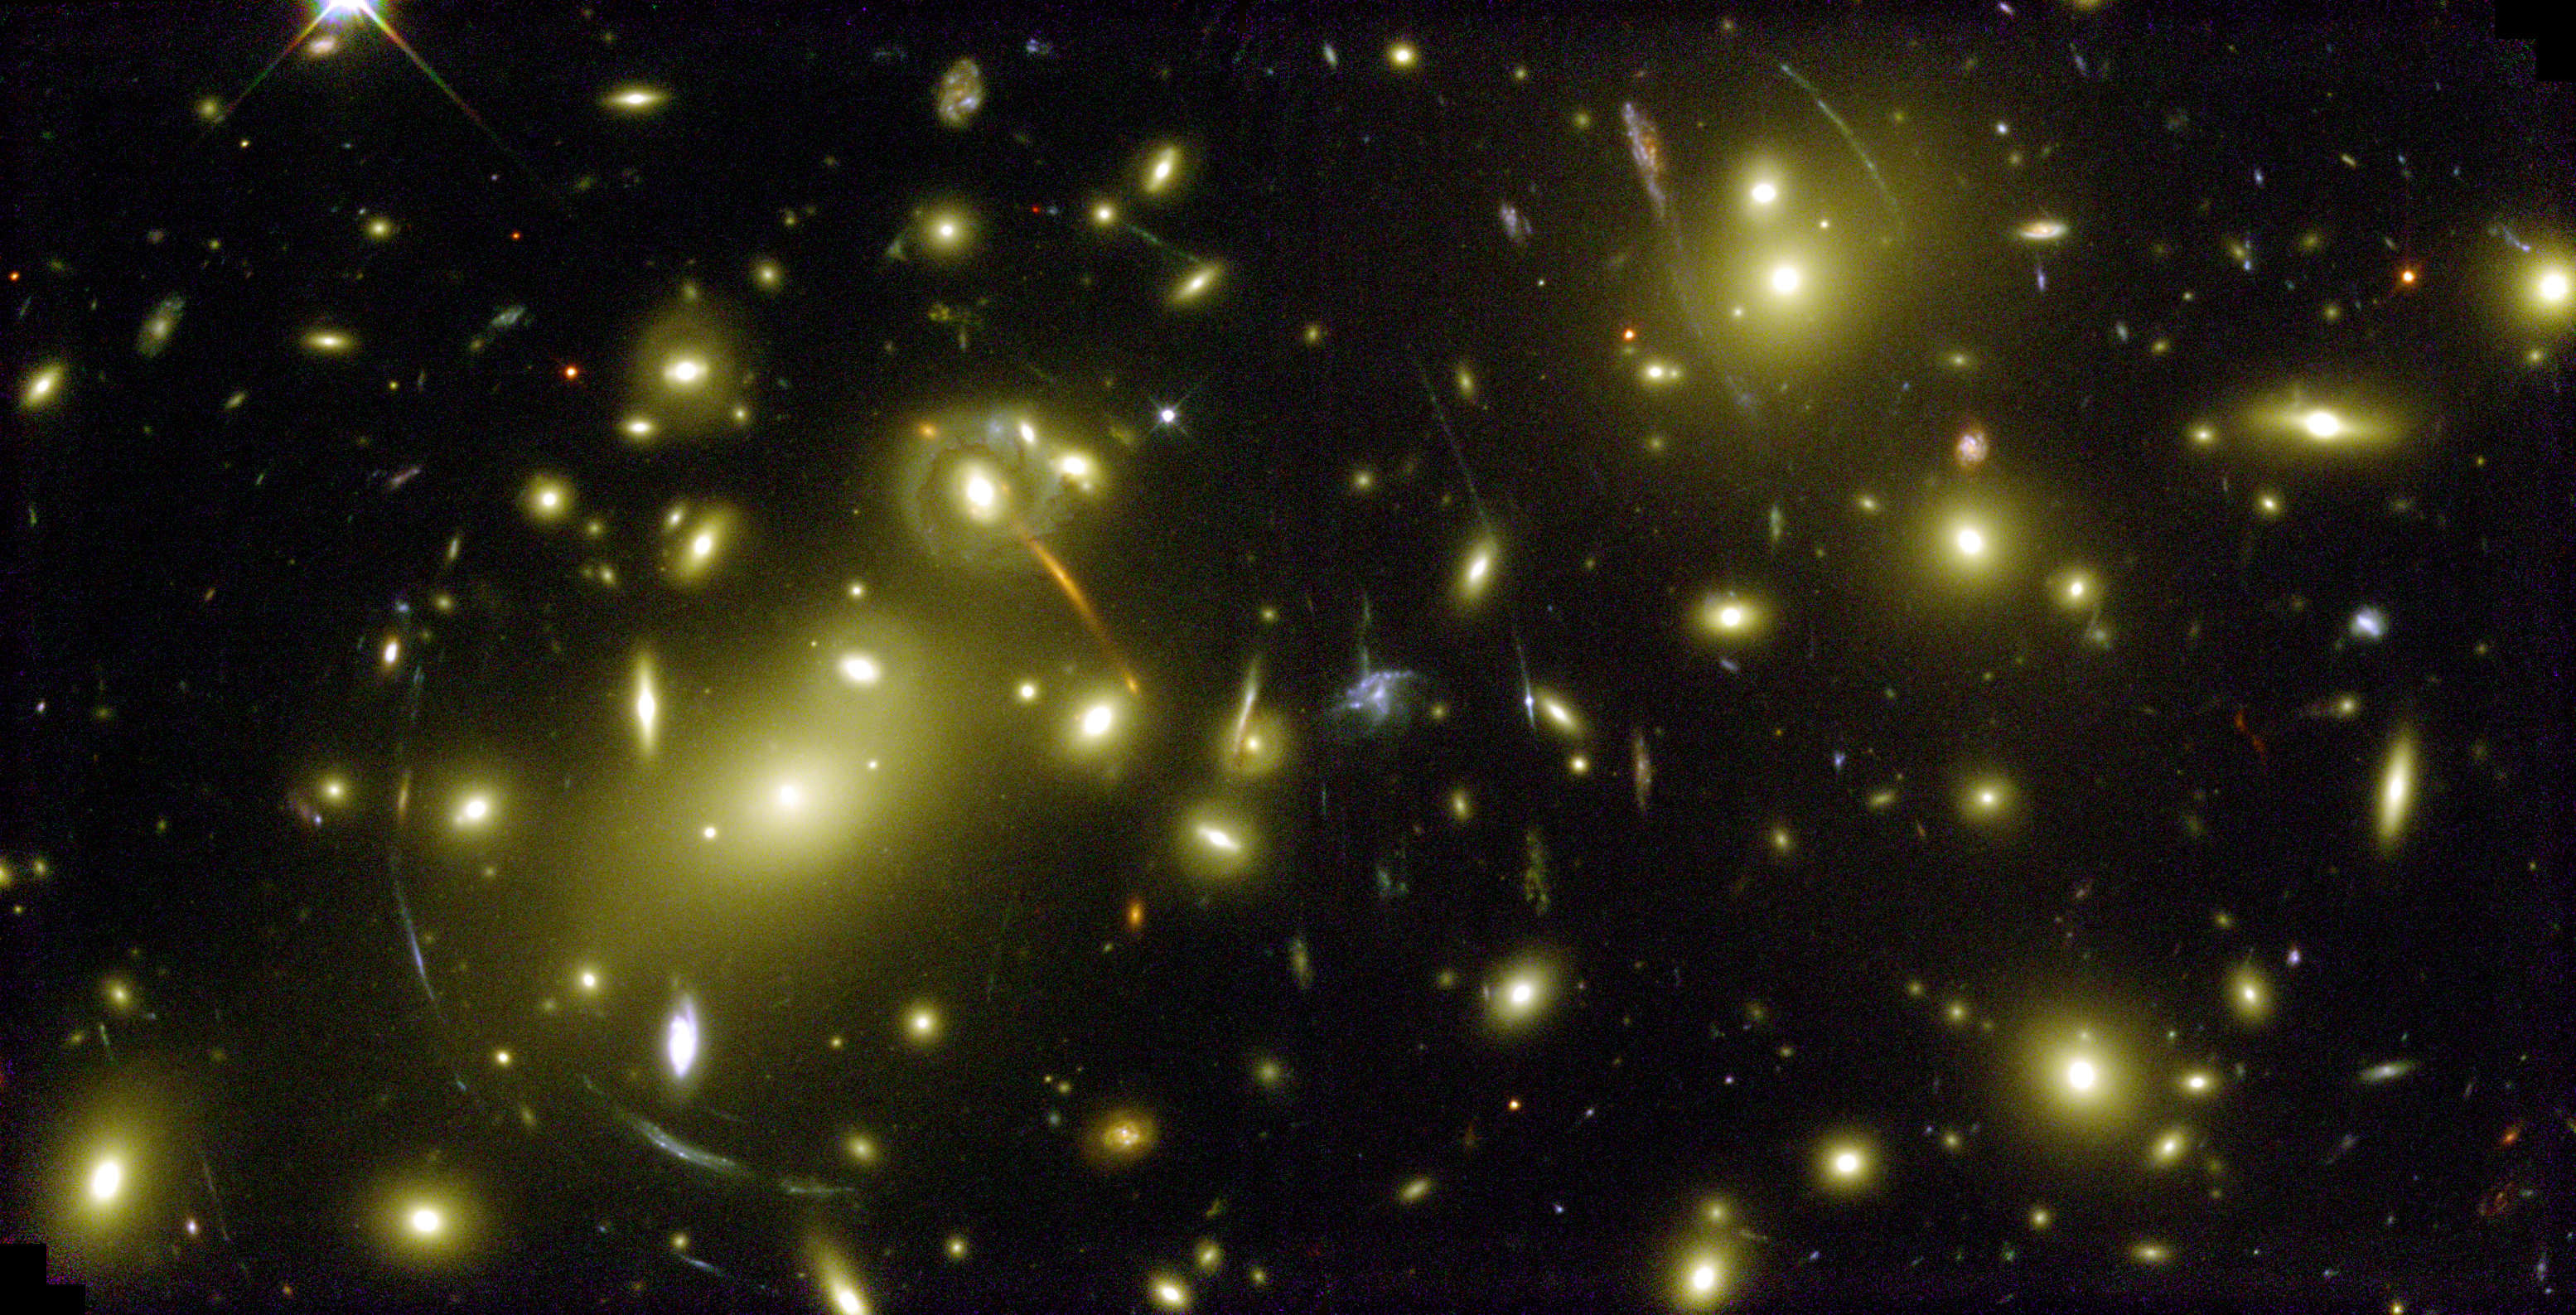
\includegraphics[width=\textwidth]{cluster/images/HSTCI_PR00-08}
  \caption{Galaxiencluster (Abell 2218; NASA, ERO Team)
    \cite{wiki:abell}}
  \label{fig:abell}
\end{figure}

\section{``Normale'' Linse}
\rhead{Normale Linse}
Zuerst einmal ein Rückblick wie eine ``normale'' Linse funktioniert.
Eine ``normale'' Linse nutzt die Brechung zwischen dem Linsenmaterial
und seiner Umgebung aus.  Durch diese Brechung kommt es zu einer
Winkeländerung des Lichtstrahls.  Bei homogenen Materialien mit
bekannten Brechungsindizes kann folgende Formel aus der geometrischen
Optik verwendet werden:

\begin{equation}
  \frac{\sin \varepsilon_1}{\sin \varepsilon_2} = \frac{n_2}{n_1}.
\end{equation}

Darin kommen die Winkel zur Oberflächennormalen im Sinus-Bruch
und die beiden Brechungsindizes vor.  Der
Brechungsindex eines Mediums \(n\), ergibt sich aus der
Lichtgeschwindigkeit im Vakuum \(c\) geteilt durch die
Lichtgeschwindigkeit \(u\) im Medium:

\begin{equation}
  n = \frac{c}{u}.
\end{equation}
\index{Brechungsindex}


\subsection{Prinzip von Huygens}
\rhead{Prinzip von Huygens}
\index{Huygens!Prinzip von}
Wie sich das Licht ausbreitet lässt sich anschaulich mit dem Prinzip
von Huygens aufzeigen.  In der Abbildung \ref{fig:huygens1} ist die
Lichtwellenausbreitung in einem homogenen Medium gezeigt.  Die
Lichtwelle (rote Linie unten) ist nach einem Zeitschritt
(\(\Delta t\)) an der mittleren Position zu finden.  Nach einem
weiteren \(\Delta t\) ist die Lichtwelle an der Position der obersten
roten Linie.  In der Abbildung bewegt sich die Lichtwelle von unten
nach oben.  Weil es sich um ein homogenes Material handelt, sind die
Abstände zwischen den Lichtwellen parallel und immer im gleichen
Abstand.  Das Prinzip von Huygens sagt nun, dass man von jedem Punkt
aus auf einer Lichtwelle (rote Linie), einen Halbkreis in
Ausbreitungsrichtung einzeichnen kann.  Der Halbkreis ist die Distanz,
welche das Licht nach \(\Delta t\) zurückgelegt hat.  Legt man nun
eine Umhüllende um die Halbkreise, erhält man die Position der
Lichtwelle zum neuen Zeitpunkt.

\begin{figure}
  \centering
  %
% Brechung nach dem Prinzip von Huygens


\begin{tikzpicture}

  
  % Delta t
  \foreach \y in {-1,0,1}
    \draw [very thick, color=red] (0,\y) -- (6,\y);

  \foreach \x in {1,2,3,4,5}
    \draw [black, fill=white] (\x,0) circle (.6mm);

  \foreach \x in {1,2,3,4,5}
    \draw [blue] (\x,0) ++ (0,1) arc (90:160:1cm)
                 (\x,0) ++ (0,1) arc (90:20:1cm);

  \draw [very thick, color=red, ->, >=stealth] (-.5,-.5) -- (-.5,0.5);
  \draw [very thick, color=red, ->, >=stealth] (6.5,-.5) -- (6.5,0.5);


\end{tikzpicture}
  \caption{Lichtwellen Ausbreitung nach dem Prinzip von Huygens.}
  \label{fig:huygens1}
\end{figure}

Hat man zwei verschiedenen homogene Materialien, kommt es zur
Brechung, welche auch mit dem Prinzip von Huygens gezeigt werden kann.
In der Abbildung \ref{fig:huygens2} kommt die Lichtwelle von oben
links.  Zum Zeitpunkt in dem die Lichtwelle die beiden Punkte \(A\)
und \(B\) bildet, berührt die Lichtwelle im Punkt \(A\) den
Materialübergang.  Zeichnet man nun die ``Bewegungs-Halbkreise'' ein,
so ist der Halbkreis ausgehend von \(B\) grösser als von \(A\).  Der
Grund dafür ist die höhere Lichtgeschwindigkeit im weissen Medium als
im blauen Medium.  Legt man von \(D\) aus die Tangente an den von
\(A\) ausgehenden Halbkreis, erhält man die Lichtwelle nach
\(\Delta t\).  Es ist gut sichtbar, dass die Lichtwelle
\(\overline{CD}\) gebrochen wurde und nicht parallel zu
\(\overline{AB}\) liegt.

\begin{figure}
  \centering
  \input{cluster/tikz/huygens2.tikz}
  \caption{Brechung nach dem Prinzip von Huygens.}
  \label{fig:huygens2}
\end{figure}

Im Fall der Gravitationslinse gibt es im Weltall natürlich keine starr
begrenzte homogene Bereiche.  Besser zum Vergleich geeignet ist die
Abbildung \ref{fig:huygens3} mit einem inhomogenen Material.  Durch
die tiefere Lichtgeschwindigkeit im blauen Material ist der Abstand
zwischen den Lichtwellen kleiner als im weissen Material, somit biegt
sich der Lichtstrahl.

Da die Lichtgeschwindigkeit in einem Gebiet mit hoher Gravitation
langsamer vergeht, biegen sich Lichtstrahlen in Richtung massen
schwere Objekte.  (Zum Beispiel könnte im Zentrum der blauen Fläche
ein Stern stehen.  Licht, welches nahe dem Stern vorbeigeht, wird in
Richtung des Sterns abgelenkt.)

\begin{figure}
  \centering
  %
% Brechung nach dem Prinzip von Huygens


\begin{tikzpicture}
  [every label/.style={color=black}]

  
  %

  \shade [inner color=blue!50!white, outer color=white] (-.6,0.55) circle (1.5cm);

  \coordinate (A) at (0,0);
  \coordinate (B) at (3,0);
  \draw [very thick, color=red] (A) -- (B);

  \path (B) ++ (97:1cm) coordinate (Bs);
  \path (Bs) ++ ($ (A)!1!187:(B) $) coordinate (As);
  \draw [very thick, color=red] (As) -- (Bs);

  \path (Bs) ++ (104:1cm) coordinate (Bss);
  \path (Bss) ++ ($ (A)!1!194:(B) $) coordinate (Ass);
  \draw [very thick, color=red] (Ass) -- (Bss);

  \draw [very thick, color=red] (A) ++ (0,-1) --++ ($ (B)-(A) $);
  \draw [very thick, color=red] (Bss) ++ (104:1cm) --++ ($ (A)!1!194:(B) $);

  
  % \fill [fill=blue!15!white] (0,0) rectangle (6,-2);
  % \draw [thick] (0,0) -- (6,0);
  % \coordinate[label=below left:$A$] (A) at (3,0);
  % \path (A) ++ (2,0) coordinate[label=below right:$D$] (D);

  % \draw [very thick, color=red, -<, >=stealth] (A) --++ (150:2.5) node(ray1Start){};
  % \path [name path=rayStart] (ray1Start.center) --++ (60:2.5);
  % \path [name path=ray2] (A) ++ (2,0) --++ (150:6);
  % \draw [very thick, color=red, name intersections={of=rayStart and ray2,
  %   by=ray2Start}, -<, >=stealth] (A) ++ (2,0) -- (ray2Start);

  % \path (ray2Start) ++ (-30:2.5) coordinate[label=above:$B$] (B);
  % \draw [color=red] (A) -- (B);


  % \draw [thick, color=blue] (A) ++ (.8,0) arc (0:-180:.8cm);
  % \draw [thick, color=blue]
  %   let \p1 = ($(B)-(D)$)
  %   in (B) ++ (-30:{veclen(\x1,\y1)}) arc (-30:140:{veclen(\x1,\y1)})
  %      (B) ++ (150:{veclen(\x1,\y1)}) coordinate (Bs)
  %      (A) ++ (150:{veclen(\x1,\y1)}) coordinate (As);

  % \draw [color=red] (As) -- (Bs);

  % \node [circle] (circleSmall) at (A) [minimum size=2*.8cm,
  %   inner sep=0]{};
  % \draw [color=red] (D) -- (tangent cs:node=circleSmall, point={(D)},
  %   solution=2) coordinate[label=below left:$C$] (C);


  % \path (C) ++ ($ (C)-(A) $) coordinate (Cs);
  % \path (D) ++ ($ (C)-(A) $) coordinate (Ds);
  % \draw [very thick, color=red, ->, >=stealth] (A) -- (C) -- ($ (C)!1.4!(Cs) $);
  % \draw [very thick, color=red, ->, >=stealth] (D) -- ($ (D)!1.4!(Ds) $);
  % \draw [color=red] (Cs) -- (Ds);

  % \foreach \point in {A,B,C,D}
  %   \draw [black, fill=white] (\point) circle (.6mm);


\end{tikzpicture}
  \caption{Brechung nach dem Prinzip von Huygens in einem inhomogen
    Material.}
  \label{fig:huygens3}
\end{figure}


\section{Gravitationslinse}
\rhead{Gravitationslinse}
\subsection{Einfluss der Gravitation auf die Zeit}
\rhead{Einfluss der Gravitation auf die Zeit}
Als Start wird die Formel \eqref{skript:kruemmung:raumzeitabstand}
\begin{equation*}
  s^2 = -c^2 (t_1-t_2)^2 + (x_1-x_2)^2 + (y_1-y_2)^2 + (z_1-z_2)^2
\end{equation*}
aus dem Abschnitt über den Lichtkegel genommen.

Die Gravitationslinse beugt Lichtwellen, somit ist \(s^2=0\), da sich
die Wirkung mit Lichtgeschwindigkeit ausbreitet.  Wird zur
Vereinfachung \(c=1\) gesetzt, ergibt sich:
\begin{equation*}
  0 = -(t_1-t_2)^2 + (x_1-x_2)^2 + (y_1-y_2)^2 + (z_1-z_2)^2
\end{equation*}
oder anders geschrieben
\begin{equation*}
  0 = -dt^2 + dx^2 + dy^2 + dz^2.
\end{equation*}

Die Lichtwellen bewegen sich in minimalen Wegen, was den Geodäten
entspricht.  Die Lichtablenkung an Sternen und Galaxien befindet sich
im Bereich von schwachen Gravitationsfeldern.  Zu diesen wurden die
\(g_{\mu\nu}\):
\begin{align*}
  g_{00} &= -1 -\frac{2\varphi}{c^2} &g_{kk} &= 1,\quad k=1,2,3
\end{align*}
bereits berechnet (Formel \ref{skript:gravitation:naeherung}).
Das Gravitationspotential \(\varphi\) ist für eine Punktmasse:
\begin{equation*}
  \varphi = -\frac{KM}{r}
\end{equation*}
\(M\) ist die Punktmasse, \(K\) die Gravitationskonstante
(oft als \(G\) bezeichnet) und \(r\) der Abstand zur Punktmasse.
Setzt man dies nun zusammen, erhält man folgende \(g_{\mu\nu}\):
\begin{align*}
  g_{00} &= -1 +\frac{2KM}{rc^2} &g_{kk} &= 1,\quad k=1,2,3.
\end{align*}
Für grosse Abstände \(r\) wird \(g_{00}=-1\).  Was gleich der normalen
Minkowski-Metrik ist.

\begin{beispiel}
  In folgendem soll die Zeitveränderung für Werte unserer Sonne
  berechnet werden.  Die Werte sind:
  \begin{align*}
    K &= \SI{6.67e-11}{\meter\cubed\per\kilogram\per\second\squared}
    &M &= \SI{1.99e30}{\kilogram}
    &c &= \SI{2.99e8}{\meter\per\second}.
  \end{align*}
  Die Zeitveränderung wird nur vom zweiten Teil von \(g_{00}\)
  bestimmt, wobei man erhält:
  \begin{align*}
    \tilde{t} &= \frac{2KM}{rc^2}
    &\left[\tilde{t}\right] &=
                              \si{\meter\cubed\per\kilogram\per\second\squared}
                              \cdot \si{\kilogram}
                              \cdot \si{\per\meter}
                              \cdot \si{\per\meter\squared\second\squared}
                              = 1.
  \end{align*}
  Einen Graphen mit den Werten von \(1\) bis \(0.05\) für
  \(\tilde{t}\) mit dem Abstand \(r\) kann in der Abbildung
  \ref{fig:bsp1} gefunden werden.  Ein \(\tilde{t}\) von \(0.25\)
  entspricht einer Verlangsamung von Wasser.  Je näher bei
  \(\tilde{t}=1\) desto langsamer bewegt sich das Licht, da
  \(g_{00} \rightarrow 0\) wird.  Es ist zu beachten, dass das
  geplotete maximale \(r\) von \SI{60000}{\meter} immer noch innerhalb
  der Sonne ist, da der Sonnenradius \SI{\approx 700e6}{\meter}
  entspricht.
  \begin{figure}
    \centering
    

\begin{tikzpicture}[scale = 1.7]
    \datavisualization[scientific axes = clean,
                     y axis = {grid,
                               label=\(\tilde{t}\) von \(1\) bis \(0.05\),
                               min value = 0,
                               max value = 1},
                     x axis = {grid,
                               label=\(r\) in \si{\meter},
                               min value = 0,
                               max value = 60000},
                     visualize as smooth line/.list={ch1},
                     style sheet=vary hue,
                     %style sheet=vary dashing,
                     %ch1={label in legend={text=Mittenkavität}},
                     ]
                    
  data [set=ch1,headline={x, y}, read from file=cluster/source/bsp1.csv];
\end{tikzpicture}
    \caption{\(\tilde{t}\) von \(1\) bis \(0.05\)}
    \label{fig:bsp1}
  \end{figure}
\end{beispiel}

Im obigen Beispiel ist gut ersichtlich, wie schnell der Einfluss der
Gravitation abnimmt.  Eine Linse mit dieser Eigenschaft müsse so
geformt sein, wie ein Weinglasboden.  In der Abbildung
\ref{fig:ModelGravLinse} sind drei Beispielkonstellationen zu sehen.
Ist der Weinglasboden in einer Linie mit der Kerze (unten links)
erhält man ein Einsteinring ähnliches Gebilde.  Bei einem gekippten
Boden (oben rechts) erhält man beinahe ein Einsteinkreuz.  Und unten
rechts sieht man ein Beispiel was passiert, wenn die Linse und die
Quelle nicht in einer Linie stehen (wie im Cluster Bild
\ref{fig:abell}).

\begin{figure}
  \centering
  \includegraphics[width=\textwidth]{cluster/images/model_grav_lens}
  \caption{Model einer Gravitationslinse (Boden eines Weinglases)
    \cite{standford:ModelGravLens}}
  \label{fig:ModelGravLinse}
\end{figure}

\subsection{Euler-Lagrange}
\rhead{Euler-Lagrange}
\index{Euler-Lagrange-Gleichungen}
Um die Lichtablenkung zu berechnen, benötigt man den Weg des Lichts
und nicht nur wie stark die Lichtgeschwindigkeit abgebremst wird.  Das
Licht nimmt den Weg mit der kürzesten Laufzeit.  Aus der Physik kennt
man, dass die Zeit gleich der Strecke durch die Geschwindigkeit ist:
\begin{equation*}
  t = \frac{s}{v}.
\end{equation*}

Für den Weg des Lichts muss man somit jedes Wegstück mit seiner
Geschwindigkeit dividieren und all diese Stückchen zusammen addieren.
Das Licht nimmt nun den Weg, in welchem es die kürzeste Laufzeit hat.
Um eine Strecke zu minimieren, kann man Euler-Lagrange verwenden,
welche ein Integral der Form
\begin{equation*}
  I = \int\limits_{t_0}^{t_1}\! F\bigl(x^{\alpha}(t), \dot{x}^{\alpha}(t),t\bigr)d t
\end{equation*}
benötigt.  Das Integral soll die Zeit minimieren, somit muss es einen
Weg geteilt durch eine Geschwindigkeit im Integral geben.  Eine
Möglichkeit ist folgendes Integral:
\begin{equation}
  I = \int\! \sqrt{\dot{x}(l)^2+\dot{y}(l)^2+\dot{z}(l)^2} \cdot
  \frac{n\bigl(x(l),y(l),z(l)\bigr)}{c} d l.
\end{equation}

Der Wert unter der Wurzel entspricht dem Wegstück während eines
Integrationsschritts.  Die Division entspricht eins durch die
Geschwindigkeit.  Somit erhält man im Integral eine Zeit, welche über
den gesamten Weg integriert der Wegzeit des Lichts entspricht.  Da die
Lichtgeschwindigkeit \(c\) unabhängig von der Position ist, kann man
den Bruch vor das Integral nehmen:
\begin{equation}
  I = \frac{1}{c}\int\! \sqrt{\dot{x}(l)^2+\dot{y}(l)^2+\dot{z}(l)^2}
  \cdot n\bigl(x(l),y(l),z(l)\bigr) d l.
\end{equation}
Des Weiteren benötigt man für Euler-Lagrange nur den Teil im Integral:
\begin{equation}
  L = \sqrt{\dot{x}(l)^2+\dot{y}(l)^2+\dot{z}(l)^2}
  \cdot n\bigl(x(l),y(l),z(l)\bigr).
\end{equation}
Da die Wurzel die folgenden Rechenschritte verkompliziert, wird sie
quadriert, was das Extremum nicht verändert.  Dieser Schritt wurde
bereits im Abschnitt
\ref{skript:geodaeten:subsection:Parametrisierung} angewendet.  Weiter
wird die Abhängigkeit von \(l\) nicht mehr geschrieben, was es
natürlich bleibt:
\begin{equation}
  F = L^2 = (\dot{x}^2+\dot{y}^2+\dot{z}^2)n^2.
\end{equation}

Für Euler-Lagrange muss man nun dieses \(F\) ableiten, im folgenden
nur mit \(x\) gezeigt:
\begin{equation}
  \label{eq:cluster:euler}
  0 = \frac{\partial F}{\partial x} - \frac{d}{d l} \frac{\partial
    F}{\partial \dot{x}}.
\end{equation}
Die Ableitungen sind
\begin{align*}
  \frac{\partial F}{\partial x} &= (\dot{x}^2+\dot{y}^2+\dot{z}^2) 2n
                                  \frac{\partial n}{\partial x}\\
  \frac{\partial F}{\partial\dot{x}} &= 2\dot{x}n^2\\
  \frac{d}{d l}\frac{\partial F}{\partial\dot{x}} &= 2\ddot{x}n^2 + 4\dot{x}n
                                \left(\frac{\partial n}{\partial x}\dot{x} +
                                \frac{\partial n}{\partial y}\dot{y} +
                                \frac{\partial n}{\partial z}\dot{z} \right).
\end{align*}
Setzt man die obigen Berechnungen in \ref{eq:cluster:euler} ein und
löst diese Formel nach \(\ddot{x}\) auf, erhält man:
\begin{equation}
  \ddot{x} = (-\dot{x}^2+\dot{y}^2+\dot{z}^2)
  \frac{1}{n}\frac{\partial n}{\partial x} -
  2\dot{x}\dot{y} \frac{1}{n}\frac{\partial n}{\partial y} -
  2\dot{x}\dot{z} \frac{1}{n}\frac{\partial n}{\partial z}.
\end{equation}
Mit der Hilfe der logarithmischen Differentiation
\begin{equation*}
  \frac{1}{n} \frac{\partial n}{\partial x} = \frac{\partial \ln
    n}{\partial x}
\end{equation*}
kann man die Formel weiter vereinfachen:
\begin{equation}
  \ddot{x} = (-\dot{x}^2+\dot{y}^2+\dot{z}^2) \frac{\partial \ln
    n}{\partial x} - 2\dot{x}\dot{y} \frac{\partial \ln n}{\partial y}
  - 2\dot{x}\dot{z} \frac{\partial \ln n}{\partial z}.
\end{equation}
Normalerweise ist ein Logarithmus nicht der einfachste Ansatz.  Die
Vereinfachung entsteht durch die spezielle Form von \(n\)
\begin{equation*}
  n \approx 1-\frac{2\varphi}{c^2}
\end{equation*}
und weil
\begin{equation*}
  \frac{\varphi}{c^2} \ll 1
\end{equation*}
ergibt sich
\begin{equation*}
  \ln n \approx -\frac{2\varphi}{c^2}.
\end{equation*}

Somit muss man nun keine partielle Ableitung von \(\ln n\), sondern von
\(-\frac{2\varphi}{c^2}\) durchführen (d.h. man braucht
\(\nabla\varphi=\) Gravitationskraft).  In einem Beispiel soll dies in
2D gezeigt werden.

\begin{beispiel}
  Im Folgenden wird die Lichtablenkung in einem zwei dimensionalen
  Raum numerisch berechnet.  Als \(\varphi\) wird eine Punktquelle
  verwendet:
  \begin{equation*}
    \varphi = -\frac{KM}{r}.
  \end{equation*}
  Wobei
  \begin{equation*}
    r = \sqrt{(x-x_L)^2+(y-y_L)^2}
  \end{equation*}
  der Abstand zwischen dem aktuellen Punkt und der Linse ist.

  Berechnet man mit Hilfe von Maxima Euler-Lagrange nach den beiden
  Koordinatenachsen, erhält man:
  \begin{align*}
    \ddot{x} &= -\frac{2(-\dot{x}^2+\dot{y}^2)(x-x_L)KM}
               {c^2\sqrt{(x-x_L)^2+y^2}\,^3}+
               \frac{4\dot{x}y\dot{y}KM}{c^2\sqrt{(x-x_L)^2+y^2}\,^3}\\
    \ddot{y} &= +\frac{4\dot{x}\dot{y}(x-x_L)KM}{c^2\sqrt{(x-x_L)^2+y^2}\,^3}
               - \frac{2(\dot{x}^2-\dot{y}^2)yKM}
               {c^2\sqrt{(x-x_L)^2+y^2}\,^3}.
  \end{align*}
  In diesem Beispiel befindet sich die Gravitationslinse auf \(x=0\),
  somit vereinfacht sich \(y-y_L\) zu \(y\).  Die soeben erhaltenen
  Formeln kann man in dieser Form noch nicht verwenden.  Man hat ein
  Differentialgleichungssystem zweiter Ordnung.  Was von geläufigen
  Computer Algorithmen nicht gelöst werden kann, da sie ein DGL-System
  erster Ordnung benötigen.

  Mit Substitution kann man eine Differentialgleichung zweiter Ordnung
  in ein DGL-System erster Ordnung überführen.  Macht man diese
  Substitution mit beiden Formeln, erhält man ein Gleichungssystem
  erster Ordnung, welche beide Formeln enthält.  Wählt man folgende
  Substitutionen
  \begin{align*}
    x_1 &= x &x_2 &= \dot{x} &x_3 &= y &x_4 &= \dot{y}
  \end{align*}
  kann man die beiden Formeln in eine brauchbare Form bringen.  Die
  gängigen Algorithmen fordern die Ableitungen von \(x_k\) als
  Parametern:
  \begin{align*}
    \dot{x}_1 &= x_2\\
    \dot{x}_2 &= -\frac{2\left(-x_2^2+x_4^2\right)\bigl(x_1-x_L\bigr)KM}
                {c^2\sqrt{\bigl(x_1-x_L\bigr)^2+x_3^2}\,^3}
                + \frac{4 x_2x_3x_4 KM}
                {c^2\sqrt{\bigl(x_1-x_L\bigr)^2+x_3^2}\,^3}\\
    \dot{x}_3 &= x_4\\
    \dot{x}_4 &= +\frac{4x_2x_4\bigl(x_1-x_L\bigr)KM}
                {c^2\sqrt{\bigl(x_1-x_L\bigr)^2+x_3^2}\,^3}
                - \frac{2 \left(x_2^2-x_4^2\right) x_3 KM}
                {c^2\sqrt{\bigl(x_1-x_L\bigr)^2+x_3^2}\,^3}.
  \end{align*}

  In Octave wird \(x_k\) zu \texttt{x(k)}, was zu folgendem Code
  führt:
  \lstinputlisting[style=Octave]{cluster/source/dglSubCode.m}

  Setzt Man nun die Werte
  \begin{align*}
    x_L &\approx \SI{150e6}{\kilo\meter} &M &\approx
                                              \SI{2e30}{\kilogram}
    &R &\approx \SI{700e3}{\kilo\meter}
  \end{align*}
  der Sonne ein,
  erhält man eine Winkeländerung von \(\approx \SI{1.75}{''}\),
  vergleicht man dies mit dem Wert aus der Literatur von
  \(\SI{1.75}{''}\) (\cite{misner1973gravitation} S.446), scheint
  dieses Vorgehen ziemlich adäquat.

  Im Graphen \ref{fig:lichtablenkungSonne} ist der numerisch
  berechnete Lichtweg dargestellt.  Der Beobachter ist im Punkt (0,0)
  und die Sonne im Punkt (\SI{1.5e11}{\meter},0).  Der Lichtpfad
  startet von der Erde aus so, dass man direkt am Sonnenradius
  vorbeischaut.  Da die Ablenkung nur \SI{1.75}{''} ist, sieht der Lichtweg
  von Auge betrachtet wie eine gerade Strecke aus.  (Eine Bogensekunde
  ist ein 3600stel eines Grades.)

  Nimmt man zur Berechnung eine schwerere Sonne an, ist die
  Lichtablenkung auch von Auge gut zu sehen.  In der Abbildung
  \ref{fig:lichtablenkung300Sonne} ist die Sonne 300 mal schwerer (bei
  gleichem Radius) und in \ref{fig:lichtablenkung600Sonne} sogar 600
  mal mehr.

  \begin{figure}
    \centering
    \begin{tikzpicture}[scale = 1.7]
      \datavisualization[scientific axes = clean,
                         y axis = {grid,
                                   label=\(y\) in \si{\meter},
                                   min value = 0,
                                   max value = 1.5e9},
                         x axis = {grid,
                                   label=\(x\) in \si{\meter},
                                   min value = 0,
                                   max value = 3e11},
                         visualize as smooth line/.list={ch1},
                         % ch1={style=very thick},
                         style sheet=vary hue,
                         % style sheet=vary dashing,
                         % ch1={label in legend={text=Mittenkavität}},
                        ]
                    
      data [set=ch1,headline={x, y}, read from file=cluster/source/lichtablenkungSonne.csv];
    \end{tikzpicture}
    \caption{Lichtablenkung an der Sonne}
    \label{fig:lichtablenkungSonne}
  \end{figure}
  
  \begin{figure}
    \centering
    \begin{tikzpicture}[scale = 1.7]
      \datavisualization[scientific axes = clean,
                         y axis = {grid,
                                   label=\(y\) in \si{\meter},
                                   min value = 0,
                                   max value = 1.5e9},
                         x axis = {grid,
                                   label=\(x\) in \si{\meter},
                                   min value = 0,
                                   max value = 3e11},
                         visualize as smooth line/.list={ch1},
                         % ch1={style=very thick},
                         style sheet=vary hue,
                         % style sheet=vary dashing,
                         % ch1={label in legend={text=Mittenkavität}},
                        ]
                    
      data [set=ch1,headline={x, y}, read from file=cluster/source/lichtablenkung300Sonne.csv];
    \end{tikzpicture}
    \caption{Lichtablenkung an 300 Sonnenmassen}
    \label{fig:lichtablenkung300Sonne}
  \end{figure}
  
  \begin{figure}
    \centering
    \begin{tikzpicture}[scale = 1.7]
      \datavisualization[scientific axes = clean,
                         y axis = {grid,
                                   label=\(y\) in \si{\meter},
                                   min value = 0,
                                   max value = 1.5e9},
                         x axis = {grid,
                                   label=\(x\) in \si{\meter},
                                   min value = 0,
                                   max value = 3e11},
                         visualize as smooth line/.list={ch1},
                         % ch1={style=very thick},
                         style sheet=vary hue,
                         % style sheet=vary dashing,
                         % ch1={label in legend={text=Mittenkavität}},
                        ]
                    
      data [set=ch1,headline={x, y}, read from file=cluster/source/lichtablenkung600Sonne.csv];
    \end{tikzpicture}
    \caption{Lichtablenkung an 600 Sonnenmassen}
    \label{fig:lichtablenkung600Sonne}
  \end{figure}
\end{beispiel}

Im vorherigen Beispiel sieht man gut, dass die Lichtstrahlen bis
praktisch zur Sonne eine Gerade darstellen, dann abgebogen werden und
wieder in einer Gerade weiterfliegen.  Stellt man nur diese Ablenkung
dar (\ref{fig:lichtablenkung600SonneZoom}) ist das noch besser
sichtbar.

\begin{figure}
  \centering
  \begin{tikzpicture}[scale = 1.7]
    \datavisualization[scientific axes = clean,
                       y axis = {grid,
                                 label=\(y\) in \si{\meter},
                                 min value = 6.5e8,
                                 max value = 7e8},
                       x axis = {grid,
                                 label=\(x\) in \si{\meter},
                                 min value = 1.4e11,
                                 max value = 1.6e11},
                       visualize as smooth line/.list={ch1},
                       % ch1={style=very thick},
                       style sheet=vary hue,
                       % style sheet=vary dashing,
                       % ch1={label in legend={text=Mittenkavität}},
                      ]
                    
    data [set=ch1,headline={x, y}, read from file=cluster/source/zoomLichtablenkung600Sonne.csv];
  \end{tikzpicture}
  \caption{Lichtablenkung an 600 Sonnenmassen (Zoom)}
  \label{fig:lichtablenkung600SonneZoom}
\end{figure}

Das Verhalten, dass über eine lange Strecke nichts passiert, erschwert
die nummerische Berechnung.  Die Algorithmen ode23 und ode45 in Octave
waren nicht in der Lage den Weg zu berechnen.  Hingegen konnte die
Lichtablenkung im Beispiel oben mit ode23s aus Octave berechnet
werden.  Dieser Algorithmus ist fähig steife Probleme zu berechnen.
Solche Probleme nennt man steif, wenn eine tiefe Frequenz von einer
hohen Frequenz überlagert wird.  Im weiteren Sinn ist dieses Problem
steif, da zwischen Beobachter, Gravitationslinse und Quelle sehr
grosse Abstände vorhanden sind, in denen nichts passiert.  Zum Lösen
berechnet ode23s auf der gesamten vorgegebenen Strecke Punkte.  Für
Sonnenabstände ist dies noch gut berechenbar, für Galaxienabstände
jedoch nicht.

\subsection{Bildverzerrung}
\rhead{Bildverzerrung}
Möchte man nun ein Bild der Lichtablenkung erzeugen, muss man für
jedes Pixel den Lichtweg simuliert.  Wenn man den einfachsten Fall der
Punktquelle beibehält, kann man die Symmetrie ausnützen und muss somit
nur ein Achtel der Pixelauflösung berechnen.

Für die Simulation wurde wieder der Abstand von der Erde zur Sonne
verwendet.  Um die Lichtablenkung noch zu verstärken, wurde die
tausendfache Sonnenmasse bei gleichem Radius angenommen.  Der
Pixelabstand in der Sonnenebene liegt bei \SI{10e6}{\meter}.  Das
Hintergrundbild, die Andromeda Galaxie aus Abbildung \ref{fig:m31},
ist in rund 6.8 fachem Sonnenabstand von der Erde aus platziert.  Der
Pixelabstand wurde gleich gewählt.

\begin{figure}
  \centering
  \includegraphics[width=\textwidth]{cluster/images/m31_comolli_2193}
  \caption{Andromeda Galaxie M31 \cite{nasa:andromedaM31}}
  \label{fig:m31}
\end{figure}

In der Abbildung \ref{fig:einsteinringSim} sieht man, wie das Zentrum
der Galaxie zu einem Ring verzogen wird.  Das schwarze Zentrum in der
Abbildung ist die Position der ``Sonne''.  Die Abbildung hat eine
Auflösung von \(300\times300\) Pixel und benötigte gut eineinhalb Tage
Berechnungszeit bei vier Kernen mit Hyper-Threading.

\begin{figure}
  \centering
  \includegraphics[width=.6\textwidth]{cluster/images/einsteinring}
  \caption{Bildverzerrung durch 1000 Sonnenmassen}
  \label{fig:einsteinringSim}
\end{figure}

\printbibliography[heading=subbibliography]
\end{refsection}


\chapter{Lichtablenkung an einem Galaxiencluster\label{chapter:thema}}
\lhead{Lichtablenkung an einem Galaxiencluster}
\begin{refsection}
\chapterauthor{Pascal Stump}

\section{Einleitung}
\rhead{Einleitung}
Wenn ein sehr massereiches Objekt zwischen einem Betrachter und einer
Lichtquelle platziert ist, tritt ein Gravitationslinseneffekt auf.  In
der Abbildung \ref{fig:lrg3-757} sieht man ein Beispiel, bei welchem
die Vordergrund-Galaxie (gelb/orange) praktisch in einer Linie zur
Hintergrund-Galaxie (blau) steht.  Durch die beinahe optimale
Ausrichtung in einer Linie wird die Hintergrund-Galaxie zu einem
Kreis verzerrt.  Der dabei entstehende Kreis wird auch Einsteinring
genannt.

Wenn die Vordergrund-Galaxie nicht rotationssymmetrisch ist, kann die
Hintergrund-Galaxie zu einzelnen Punkten verzerrt werden, so zu sehen
in der Abbildung \ref{fig:einsteinkreuz}.  Dabei ist die
Vordergrund-Galaxie wieder in der Mitte zu finden und die vier
umliegenden Punkte sind die verzerrte Hintergrund-Galaxie.

Ein drittes Beispiel des Gravitationslinseneffekts ist in Abbildung
\ref{fig:abell} zu finden.  Dabei ist nicht nur eine Galaxie als Linse
zuständig, sondern ein Galaxiencluster.  Die Vordergrund-Galaxien ist
wiederum die gelb, orange farbigen Galaxien.  Man sieht schön, dass
die Hintergrund-Galaxien zu Streifen verzogen werden und nicht mehr zu
einem ganzen Kreis, da die Ausrichtungen zueinander nicht optimal
sind.

\begin{figure}
  \centering
  \includegraphics[width=\textwidth]{cluster/images/LRG_3-757}
  \caption{Einsteinring (LRG 3-757; ESA/Hubble \& NASA)
    \cite{nasa:einsteinring, wiki:einsteinring}}
  \label{fig:lrg3-757}
\end{figure}

\begin{figure}
  \centering
  \includegraphics[width=.7\textwidth]{cluster/images/Einstein_cross}
  \caption{Einsteinkreuz (G2237+0305; NASA, ESA \& STScl)
    \cite{wiki:einsteinkreuz}}
  \label{fig:einsteinkreuz}
\end{figure}

\begin{figure}
  \centering
  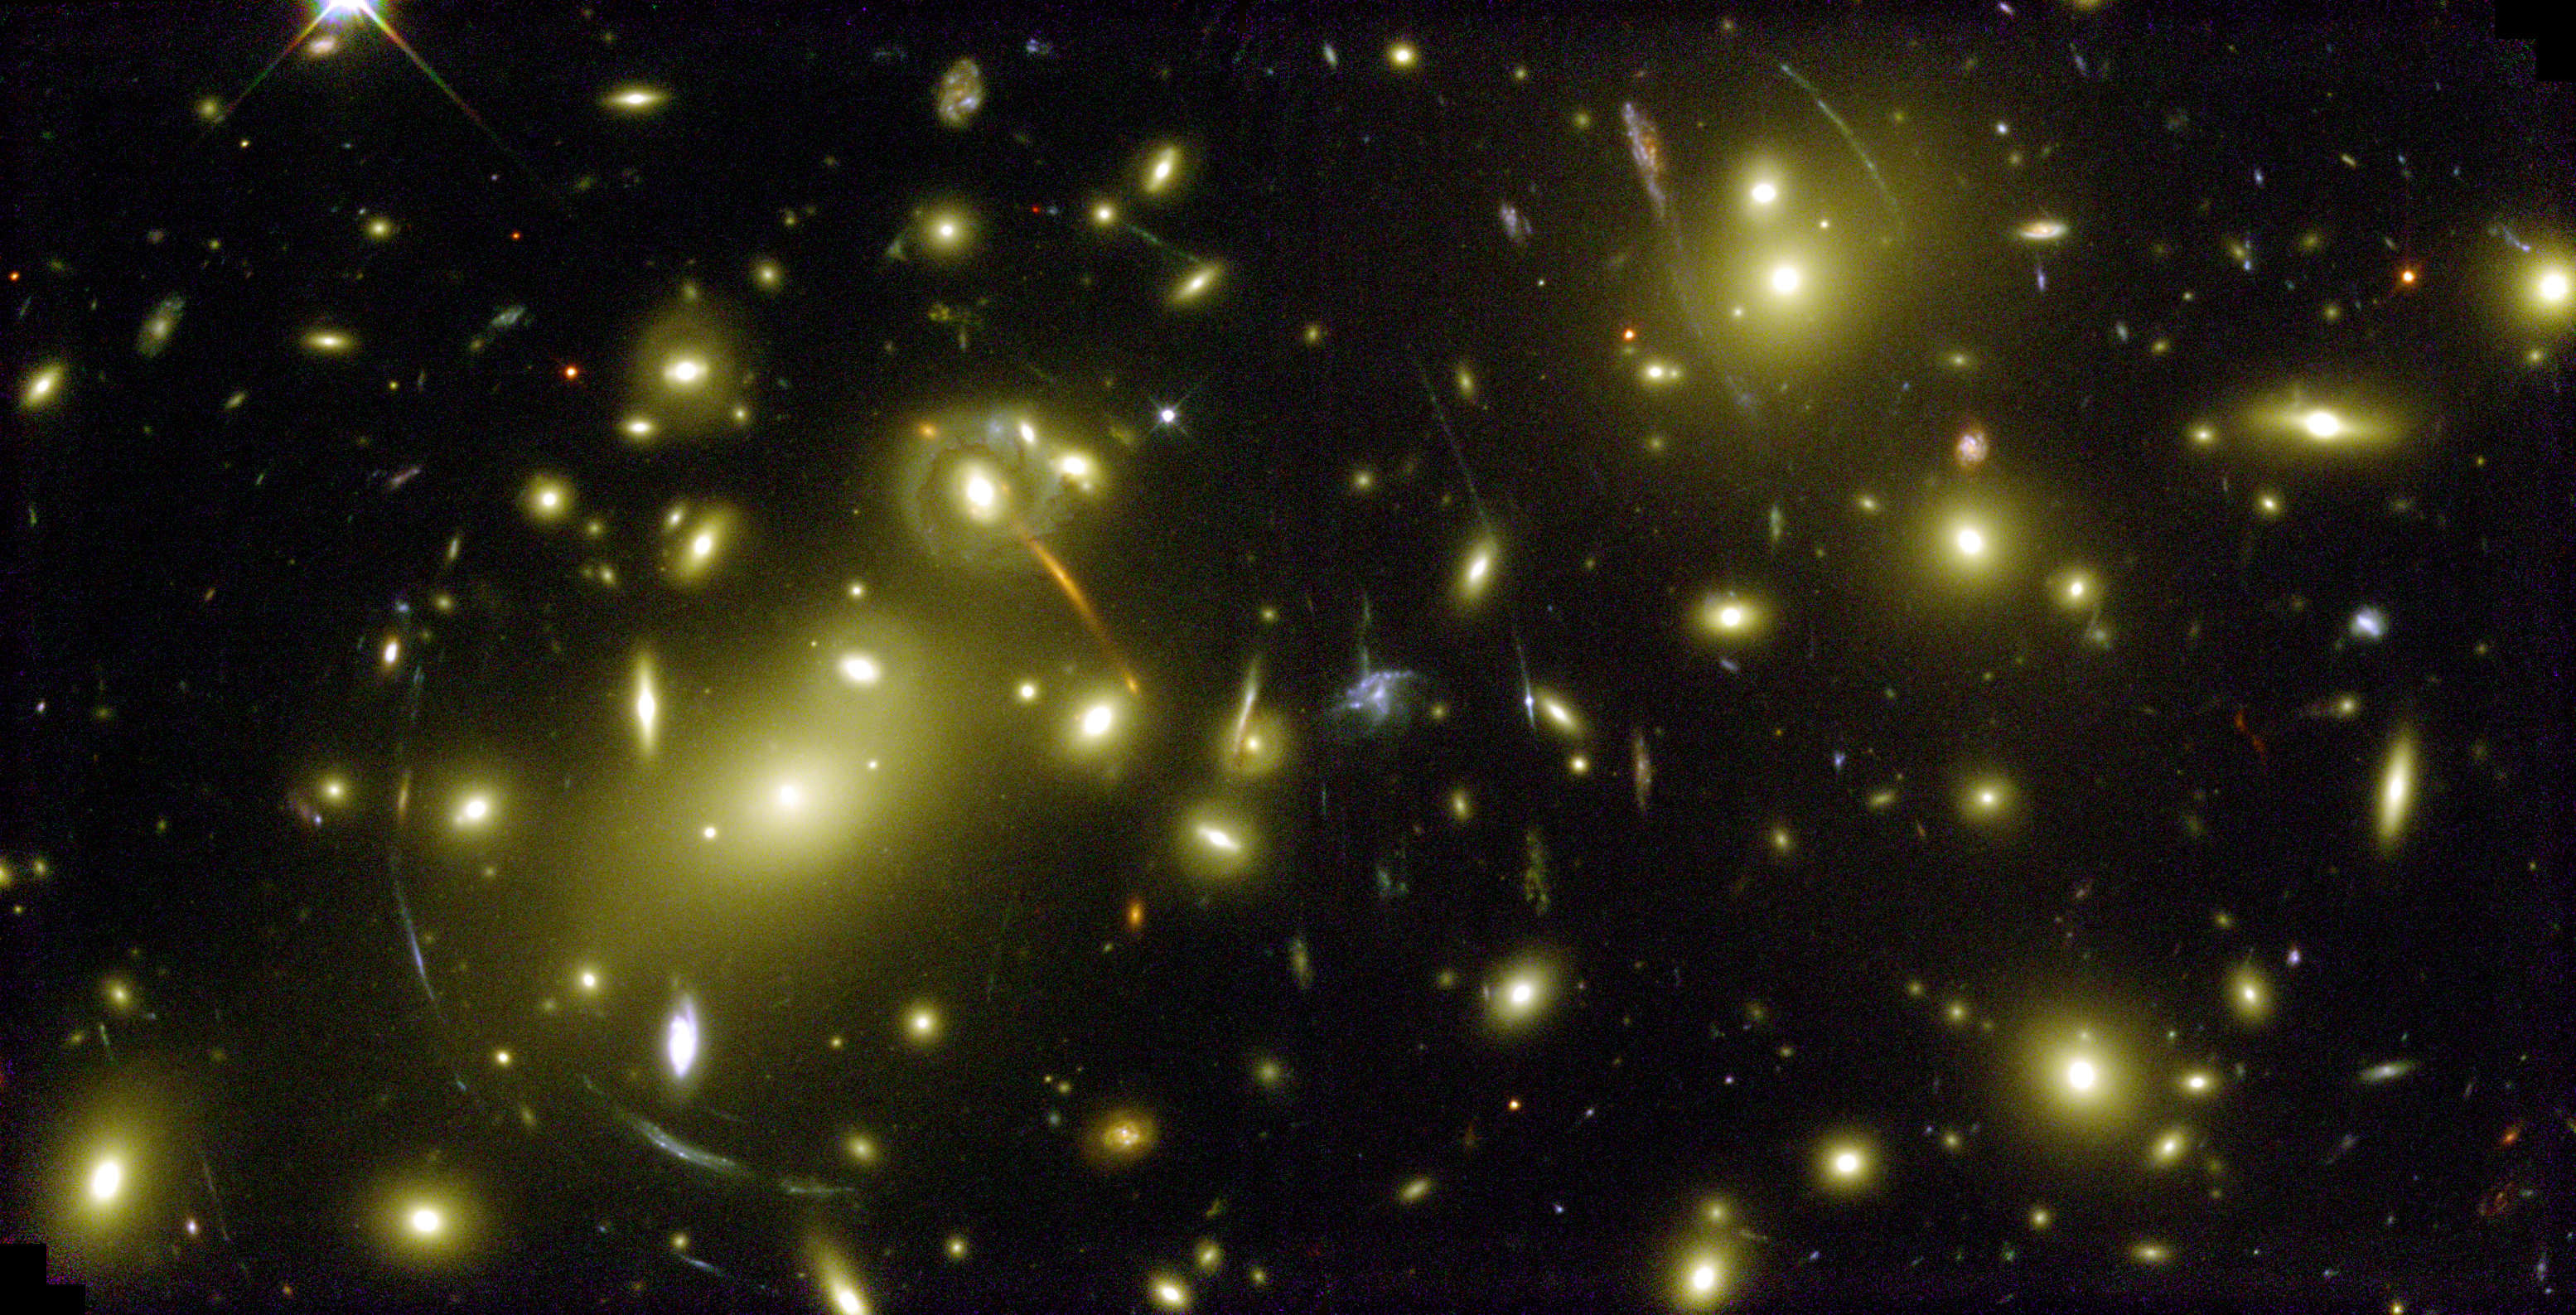
\includegraphics[width=\textwidth]{cluster/images/HSTCI_PR00-08}
  \caption{Galaxiencluster (Abell 2218; NASA, ERO Team)
    \cite{wiki:abell}}
  \label{fig:abell}
\end{figure}

\section{``Normale'' Linse}
\rhead{Normale Linse}
Zuerst einmal ein Rückblick wie eine ``normale'' Linse funktioniert.
Eine ``normale'' Linse nutzt die Brechung zwischen dem Linsenmaterial
und seiner Umgebung aus.  Durch diese Brechung kommt es zu einer
Winkeländerung des Lichtstrahls.  Bei homogenen Materialien mit
bekannten Brechungsindizes kann folgende Formel aus der geometrischen
Optik verwendet werden:

\begin{equation}
  \frac{\sin \varepsilon_1}{\sin \varepsilon_2} = \frac{n_2}{n_1}.
\end{equation}

Darin kommen die Winkel zur Oberflächennormalen im Sinus-Bruch
und die beiden Brechungsindizes vor.  Der
Brechungsindex eines Mediums \(n\), ergibt sich aus der
Lichtgeschwindigkeit im Vakuum \(c\) geteilt durch die
Lichtgeschwindigkeit \(u\) im Medium:

\begin{equation}
  n = \frac{c}{u}.
\end{equation}
\index{Brechungsindex}


\subsection{Prinzip von Huygens}
\rhead{Prinzip von Huygens}
\index{Huygens!Prinzip von}
Wie sich das Licht ausbreitet lässt sich anschaulich mit dem Prinzip
von Huygens aufzeigen.  In der Abbildung \ref{fig:huygens1} ist die
Lichtwellenausbreitung in einem homogenen Medium gezeigt.  Die
Lichtwelle (rote Linie unten) ist nach einem Zeitschritt
(\(\Delta t\)) an der mittleren Position zu finden.  Nach einem
weiteren \(\Delta t\) ist die Lichtwelle an der Position der obersten
roten Linie.  In der Abbildung bewegt sich die Lichtwelle von unten
nach oben.  Weil es sich um ein homogenes Material handelt, sind die
Abstände zwischen den Lichtwellen parallel und immer im gleichen
Abstand.  Das Prinzip von Huygens sagt nun, dass man von jedem Punkt
aus auf einer Lichtwelle (rote Linie), einen Halbkreis in
Ausbreitungsrichtung einzeichnen kann.  Der Halbkreis ist die Distanz,
welche das Licht nach \(\Delta t\) zurückgelegt hat.  Legt man nun
eine Umhüllende um die Halbkreise, erhält man die Position der
Lichtwelle zum neuen Zeitpunkt.

\begin{figure}
  \centering
  %
% Brechung nach dem Prinzip von Huygens


\begin{tikzpicture}

  
  % Delta t
  \foreach \y in {-1,0,1}
    \draw [very thick, color=red] (0,\y) -- (6,\y);

  \foreach \x in {1,2,3,4,5}
    \draw [black, fill=white] (\x,0) circle (.6mm);

  \foreach \x in {1,2,3,4,5}
    \draw [blue] (\x,0) ++ (0,1) arc (90:160:1cm)
                 (\x,0) ++ (0,1) arc (90:20:1cm);

  \draw [very thick, color=red, ->, >=stealth] (-.5,-.5) -- (-.5,0.5);
  \draw [very thick, color=red, ->, >=stealth] (6.5,-.5) -- (6.5,0.5);


\end{tikzpicture}
  \caption{Lichtwellen Ausbreitung nach dem Prinzip von Huygens.}
  \label{fig:huygens1}
\end{figure}

Hat man zwei verschiedenen homogene Materialien, kommt es zur
Brechung, welche auch mit dem Prinzip von Huygens gezeigt werden kann.
In der Abbildung \ref{fig:huygens2} kommt die Lichtwelle von oben
links.  Zum Zeitpunkt in dem die Lichtwelle die beiden Punkte \(A\)
und \(B\) bildet, berührt die Lichtwelle im Punkt \(A\) den
Materialübergang.  Zeichnet man nun die ``Bewegungs-Halbkreise'' ein,
so ist der Halbkreis ausgehend von \(B\) grösser als von \(A\).  Der
Grund dafür ist die höhere Lichtgeschwindigkeit im weissen Medium als
im blauen Medium.  Legt man von \(D\) aus die Tangente an den von
\(A\) ausgehenden Halbkreis, erhält man die Lichtwelle nach
\(\Delta t\).  Es ist gut sichtbar, dass die Lichtwelle
\(\overline{CD}\) gebrochen wurde und nicht parallel zu
\(\overline{AB}\) liegt.

\begin{figure}
  \centering
  \input{cluster/tikz/huygens2.tikz}
  \caption{Brechung nach dem Prinzip von Huygens.}
  \label{fig:huygens2}
\end{figure}

Im Fall der Gravitationslinse gibt es im Weltall natürlich keine starr
begrenzte homogene Bereiche.  Besser zum Vergleich geeignet ist die
Abbildung \ref{fig:huygens3} mit einem inhomogenen Material.  Durch
die tiefere Lichtgeschwindigkeit im blauen Material ist der Abstand
zwischen den Lichtwellen kleiner als im weissen Material, somit biegt
sich der Lichtstrahl.

Da die Lichtgeschwindigkeit in einem Gebiet mit hoher Gravitation
langsamer vergeht, biegen sich Lichtstrahlen in Richtung massen
schwere Objekte.  (Zum Beispiel könnte im Zentrum der blauen Fläche
ein Stern stehen.  Licht, welches nahe dem Stern vorbeigeht, wird in
Richtung des Sterns abgelenkt.)

\begin{figure}
  \centering
  %
% Brechung nach dem Prinzip von Huygens


\begin{tikzpicture}
  [every label/.style={color=black}]

  
  %

  \shade [inner color=blue!50!white, outer color=white] (-.6,0.55) circle (1.5cm);

  \coordinate (A) at (0,0);
  \coordinate (B) at (3,0);
  \draw [very thick, color=red] (A) -- (B);

  \path (B) ++ (97:1cm) coordinate (Bs);
  \path (Bs) ++ ($ (A)!1!187:(B) $) coordinate (As);
  \draw [very thick, color=red] (As) -- (Bs);

  \path (Bs) ++ (104:1cm) coordinate (Bss);
  \path (Bss) ++ ($ (A)!1!194:(B) $) coordinate (Ass);
  \draw [very thick, color=red] (Ass) -- (Bss);

  \draw [very thick, color=red] (A) ++ (0,-1) --++ ($ (B)-(A) $);
  \draw [very thick, color=red] (Bss) ++ (104:1cm) --++ ($ (A)!1!194:(B) $);

  
  % \fill [fill=blue!15!white] (0,0) rectangle (6,-2);
  % \draw [thick] (0,0) -- (6,0);
  % \coordinate[label=below left:$A$] (A) at (3,0);
  % \path (A) ++ (2,0) coordinate[label=below right:$D$] (D);

  % \draw [very thick, color=red, -<, >=stealth] (A) --++ (150:2.5) node(ray1Start){};
  % \path [name path=rayStart] (ray1Start.center) --++ (60:2.5);
  % \path [name path=ray2] (A) ++ (2,0) --++ (150:6);
  % \draw [very thick, color=red, name intersections={of=rayStart and ray2,
  %   by=ray2Start}, -<, >=stealth] (A) ++ (2,0) -- (ray2Start);

  % \path (ray2Start) ++ (-30:2.5) coordinate[label=above:$B$] (B);
  % \draw [color=red] (A) -- (B);


  % \draw [thick, color=blue] (A) ++ (.8,0) arc (0:-180:.8cm);
  % \draw [thick, color=blue]
  %   let \p1 = ($(B)-(D)$)
  %   in (B) ++ (-30:{veclen(\x1,\y1)}) arc (-30:140:{veclen(\x1,\y1)})
  %      (B) ++ (150:{veclen(\x1,\y1)}) coordinate (Bs)
  %      (A) ++ (150:{veclen(\x1,\y1)}) coordinate (As);

  % \draw [color=red] (As) -- (Bs);

  % \node [circle] (circleSmall) at (A) [minimum size=2*.8cm,
  %   inner sep=0]{};
  % \draw [color=red] (D) -- (tangent cs:node=circleSmall, point={(D)},
  %   solution=2) coordinate[label=below left:$C$] (C);


  % \path (C) ++ ($ (C)-(A) $) coordinate (Cs);
  % \path (D) ++ ($ (C)-(A) $) coordinate (Ds);
  % \draw [very thick, color=red, ->, >=stealth] (A) -- (C) -- ($ (C)!1.4!(Cs) $);
  % \draw [very thick, color=red, ->, >=stealth] (D) -- ($ (D)!1.4!(Ds) $);
  % \draw [color=red] (Cs) -- (Ds);

  % \foreach \point in {A,B,C,D}
  %   \draw [black, fill=white] (\point) circle (.6mm);


\end{tikzpicture}
  \caption{Brechung nach dem Prinzip von Huygens in einem inhomogen
    Material.}
  \label{fig:huygens3}
\end{figure}


\section{Gravitationslinse}
\rhead{Gravitationslinse}
\subsection{Einfluss der Gravitation auf die Zeit}
\rhead{Einfluss der Gravitation auf die Zeit}
Als Start wird die Formel \eqref{skript:kruemmung:raumzeitabstand}
\begin{equation*}
  s^2 = -c^2 (t_1-t_2)^2 + (x_1-x_2)^2 + (y_1-y_2)^2 + (z_1-z_2)^2
\end{equation*}
aus dem Abschnitt über den Lichtkegel genommen.

Die Gravitationslinse beugt Lichtwellen, somit ist \(s^2=0\), da sich
die Wirkung mit Lichtgeschwindigkeit ausbreitet.  Wird zur
Vereinfachung \(c=1\) gesetzt, ergibt sich:
\begin{equation*}
  0 = -(t_1-t_2)^2 + (x_1-x_2)^2 + (y_1-y_2)^2 + (z_1-z_2)^2
\end{equation*}
oder anders geschrieben
\begin{equation*}
  0 = -dt^2 + dx^2 + dy^2 + dz^2.
\end{equation*}

Die Lichtwellen bewegen sich in minimalen Wegen, was den Geodäten
entspricht.  Die Lichtablenkung an Sternen und Galaxien befindet sich
im Bereich von schwachen Gravitationsfeldern.  Zu diesen wurden die
\(g_{\mu\nu}\):
\begin{align*}
  g_{00} &= -1 -\frac{2\varphi}{c^2} &g_{kk} &= 1,\quad k=1,2,3
\end{align*}
bereits berechnet (Formel \ref{skript:gravitation:naeherung}).
Das Gravitationspotential \(\varphi\) ist für eine Punktmasse:
\begin{equation*}
  \varphi = -\frac{KM}{r}
\end{equation*}
\(M\) ist die Punktmasse, \(K\) die Gravitationskonstante
(oft als \(G\) bezeichnet) und \(r\) der Abstand zur Punktmasse.
Setzt man dies nun zusammen, erhält man folgende \(g_{\mu\nu}\):
\begin{align*}
  g_{00} &= -1 +\frac{2KM}{rc^2} &g_{kk} &= 1,\quad k=1,2,3.
\end{align*}
Für grosse Abstände \(r\) wird \(g_{00}=-1\).  Was gleich der normalen
Minkowski-Metrik ist.

\begin{beispiel}
  In folgendem soll die Zeitveränderung für Werte unserer Sonne
  berechnet werden.  Die Werte sind:
  \begin{align*}
    K &= \SI{6.67e-11}{\meter\cubed\per\kilogram\per\second\squared}
    &M &= \SI{1.99e30}{\kilogram}
    &c &= \SI{2.99e8}{\meter\per\second}.
  \end{align*}
  Die Zeitveränderung wird nur vom zweiten Teil von \(g_{00}\)
  bestimmt, wobei man erhält:
  \begin{align*}
    \tilde{t} &= \frac{2KM}{rc^2}
    &\left[\tilde{t}\right] &=
                              \si{\meter\cubed\per\kilogram\per\second\squared}
                              \cdot \si{\kilogram}
                              \cdot \si{\per\meter}
                              \cdot \si{\per\meter\squared\second\squared}
                              = 1.
  \end{align*}
  Einen Graphen mit den Werten von \(1\) bis \(0.05\) für
  \(\tilde{t}\) mit dem Abstand \(r\) kann in der Abbildung
  \ref{fig:bsp1} gefunden werden.  Ein \(\tilde{t}\) von \(0.25\)
  entspricht einer Verlangsamung von Wasser.  Je näher bei
  \(\tilde{t}=1\) desto langsamer bewegt sich das Licht, da
  \(g_{00} \rightarrow 0\) wird.  Es ist zu beachten, dass das
  geplotete maximale \(r\) von \SI{60000}{\meter} immer noch innerhalb
  der Sonne ist, da der Sonnenradius \SI{\approx 700e6}{\meter}
  entspricht.
  \begin{figure}
    \centering
    

\begin{tikzpicture}[scale = 1.7]
    \datavisualization[scientific axes = clean,
                     y axis = {grid,
                               label=\(\tilde{t}\) von \(1\) bis \(0.05\),
                               min value = 0,
                               max value = 1},
                     x axis = {grid,
                               label=\(r\) in \si{\meter},
                               min value = 0,
                               max value = 60000},
                     visualize as smooth line/.list={ch1},
                     style sheet=vary hue,
                     %style sheet=vary dashing,
                     %ch1={label in legend={text=Mittenkavität}},
                     ]
                    
  data [set=ch1,headline={x, y}, read from file=cluster/source/bsp1.csv];
\end{tikzpicture}
    \caption{\(\tilde{t}\) von \(1\) bis \(0.05\)}
    \label{fig:bsp1}
  \end{figure}
\end{beispiel}

Im obigen Beispiel ist gut ersichtlich, wie schnell der Einfluss der
Gravitation abnimmt.  Eine Linse mit dieser Eigenschaft müsse so
geformt sein, wie ein Weinglasboden.  In der Abbildung
\ref{fig:ModelGravLinse} sind drei Beispielkonstellationen zu sehen.
Ist der Weinglasboden in einer Linie mit der Kerze (unten links)
erhält man ein Einsteinring ähnliches Gebilde.  Bei einem gekippten
Boden (oben rechts) erhält man beinahe ein Einsteinkreuz.  Und unten
rechts sieht man ein Beispiel was passiert, wenn die Linse und die
Quelle nicht in einer Linie stehen (wie im Cluster Bild
\ref{fig:abell}).

\begin{figure}
  \centering
  \includegraphics[width=\textwidth]{cluster/images/model_grav_lens}
  \caption{Model einer Gravitationslinse (Boden eines Weinglases)
    \cite{standford:ModelGravLens}}
  \label{fig:ModelGravLinse}
\end{figure}

\subsection{Euler-Lagrange}
\rhead{Euler-Lagrange}
\index{Euler-Lagrange-Gleichungen}
Um die Lichtablenkung zu berechnen, benötigt man den Weg des Lichts
und nicht nur wie stark die Lichtgeschwindigkeit abgebremst wird.  Das
Licht nimmt den Weg mit der kürzesten Laufzeit.  Aus der Physik kennt
man, dass die Zeit gleich der Strecke durch die Geschwindigkeit ist:
\begin{equation*}
  t = \frac{s}{v}.
\end{equation*}

Für den Weg des Lichts muss man somit jedes Wegstück mit seiner
Geschwindigkeit dividieren und all diese Stückchen zusammen addieren.
Das Licht nimmt nun den Weg, in welchem es die kürzeste Laufzeit hat.
Um eine Strecke zu minimieren, kann man Euler-Lagrange verwenden,
welche ein Integral der Form
\begin{equation*}
  I = \int\limits_{t_0}^{t_1}\! F\bigl(x^{\alpha}(t), \dot{x}^{\alpha}(t),t\bigr)d t
\end{equation*}
benötigt.  Das Integral soll die Zeit minimieren, somit muss es einen
Weg geteilt durch eine Geschwindigkeit im Integral geben.  Eine
Möglichkeit ist folgendes Integral:
\begin{equation}
  I = \int\! \sqrt{\dot{x}(l)^2+\dot{y}(l)^2+\dot{z}(l)^2} \cdot
  \frac{n\bigl(x(l),y(l),z(l)\bigr)}{c} d l.
\end{equation}

Der Wert unter der Wurzel entspricht dem Wegstück während eines
Integrationsschritts.  Die Division entspricht eins durch die
Geschwindigkeit.  Somit erhält man im Integral eine Zeit, welche über
den gesamten Weg integriert der Wegzeit des Lichts entspricht.  Da die
Lichtgeschwindigkeit \(c\) unabhängig von der Position ist, kann man
den Bruch vor das Integral nehmen:
\begin{equation}
  I = \frac{1}{c}\int\! \sqrt{\dot{x}(l)^2+\dot{y}(l)^2+\dot{z}(l)^2}
  \cdot n\bigl(x(l),y(l),z(l)\bigr) d l.
\end{equation}
Des Weiteren benötigt man für Euler-Lagrange nur den Teil im Integral:
\begin{equation}
  L = \sqrt{\dot{x}(l)^2+\dot{y}(l)^2+\dot{z}(l)^2}
  \cdot n\bigl(x(l),y(l),z(l)\bigr).
\end{equation}
Da die Wurzel die folgenden Rechenschritte verkompliziert, wird sie
quadriert, was das Extremum nicht verändert.  Dieser Schritt wurde
bereits im Abschnitt
\ref{skript:geodaeten:subsection:Parametrisierung} angewendet.  Weiter
wird die Abhängigkeit von \(l\) nicht mehr geschrieben, was es
natürlich bleibt:
\begin{equation}
  F = L^2 = (\dot{x}^2+\dot{y}^2+\dot{z}^2)n^2.
\end{equation}

Für Euler-Lagrange muss man nun dieses \(F\) ableiten, im folgenden
nur mit \(x\) gezeigt:
\begin{equation}
  \label{eq:cluster:euler}
  0 = \frac{\partial F}{\partial x} - \frac{d}{d l} \frac{\partial
    F}{\partial \dot{x}}.
\end{equation}
Die Ableitungen sind
\begin{align*}
  \frac{\partial F}{\partial x} &= (\dot{x}^2+\dot{y}^2+\dot{z}^2) 2n
                                  \frac{\partial n}{\partial x}\\
  \frac{\partial F}{\partial\dot{x}} &= 2\dot{x}n^2\\
  \frac{d}{d l}\frac{\partial F}{\partial\dot{x}} &= 2\ddot{x}n^2 + 4\dot{x}n
                                \left(\frac{\partial n}{\partial x}\dot{x} +
                                \frac{\partial n}{\partial y}\dot{y} +
                                \frac{\partial n}{\partial z}\dot{z} \right).
\end{align*}
Setzt man die obigen Berechnungen in \ref{eq:cluster:euler} ein und
löst diese Formel nach \(\ddot{x}\) auf, erhält man:
\begin{equation}
  \ddot{x} = (-\dot{x}^2+\dot{y}^2+\dot{z}^2)
  \frac{1}{n}\frac{\partial n}{\partial x} -
  2\dot{x}\dot{y} \frac{1}{n}\frac{\partial n}{\partial y} -
  2\dot{x}\dot{z} \frac{1}{n}\frac{\partial n}{\partial z}.
\end{equation}
Mit der Hilfe der logarithmischen Differentiation
\begin{equation*}
  \frac{1}{n} \frac{\partial n}{\partial x} = \frac{\partial \ln
    n}{\partial x}
\end{equation*}
kann man die Formel weiter vereinfachen:
\begin{equation}
  \ddot{x} = (-\dot{x}^2+\dot{y}^2+\dot{z}^2) \frac{\partial \ln
    n}{\partial x} - 2\dot{x}\dot{y} \frac{\partial \ln n}{\partial y}
  - 2\dot{x}\dot{z} \frac{\partial \ln n}{\partial z}.
\end{equation}
Normalerweise ist ein Logarithmus nicht der einfachste Ansatz.  Die
Vereinfachung entsteht durch die spezielle Form von \(n\)
\begin{equation*}
  n \approx 1-\frac{2\varphi}{c^2}
\end{equation*}
und weil
\begin{equation*}
  \frac{\varphi}{c^2} \ll 1
\end{equation*}
ergibt sich
\begin{equation*}
  \ln n \approx -\frac{2\varphi}{c^2}.
\end{equation*}

Somit muss man nun keine partielle Ableitung von \(\ln n\), sondern von
\(-\frac{2\varphi}{c^2}\) durchführen (d.h. man braucht
\(\nabla\varphi=\) Gravitationskraft).  In einem Beispiel soll dies in
2D gezeigt werden.

\begin{beispiel}
  Im Folgenden wird die Lichtablenkung in einem zwei dimensionalen
  Raum numerisch berechnet.  Als \(\varphi\) wird eine Punktquelle
  verwendet:
  \begin{equation*}
    \varphi = -\frac{KM}{r}.
  \end{equation*}
  Wobei
  \begin{equation*}
    r = \sqrt{(x-x_L)^2+(y-y_L)^2}
  \end{equation*}
  der Abstand zwischen dem aktuellen Punkt und der Linse ist.

  Berechnet man mit Hilfe von Maxima Euler-Lagrange nach den beiden
  Koordinatenachsen, erhält man:
  \begin{align*}
    \ddot{x} &= -\frac{2(-\dot{x}^2+\dot{y}^2)(x-x_L)KM}
               {c^2\sqrt{(x-x_L)^2+y^2}\,^3}+
               \frac{4\dot{x}y\dot{y}KM}{c^2\sqrt{(x-x_L)^2+y^2}\,^3}\\
    \ddot{y} &= +\frac{4\dot{x}\dot{y}(x-x_L)KM}{c^2\sqrt{(x-x_L)^2+y^2}\,^3}
               - \frac{2(\dot{x}^2-\dot{y}^2)yKM}
               {c^2\sqrt{(x-x_L)^2+y^2}\,^3}.
  \end{align*}
  In diesem Beispiel befindet sich die Gravitationslinse auf \(x=0\),
  somit vereinfacht sich \(y-y_L\) zu \(y\).  Die soeben erhaltenen
  Formeln kann man in dieser Form noch nicht verwenden.  Man hat ein
  Differentialgleichungssystem zweiter Ordnung.  Was von geläufigen
  Computer Algorithmen nicht gelöst werden kann, da sie ein DGL-System
  erster Ordnung benötigen.

  Mit Substitution kann man eine Differentialgleichung zweiter Ordnung
  in ein DGL-System erster Ordnung überführen.  Macht man diese
  Substitution mit beiden Formeln, erhält man ein Gleichungssystem
  erster Ordnung, welche beide Formeln enthält.  Wählt man folgende
  Substitutionen
  \begin{align*}
    x_1 &= x &x_2 &= \dot{x} &x_3 &= y &x_4 &= \dot{y}
  \end{align*}
  kann man die beiden Formeln in eine brauchbare Form bringen.  Die
  gängigen Algorithmen fordern die Ableitungen von \(x_k\) als
  Parametern:
  \begin{align*}
    \dot{x}_1 &= x_2\\
    \dot{x}_2 &= -\frac{2\left(-x_2^2+x_4^2\right)\bigl(x_1-x_L\bigr)KM}
                {c^2\sqrt{\bigl(x_1-x_L\bigr)^2+x_3^2}\,^3}
                + \frac{4 x_2x_3x_4 KM}
                {c^2\sqrt{\bigl(x_1-x_L\bigr)^2+x_3^2}\,^3}\\
    \dot{x}_3 &= x_4\\
    \dot{x}_4 &= +\frac{4x_2x_4\bigl(x_1-x_L\bigr)KM}
                {c^2\sqrt{\bigl(x_1-x_L\bigr)^2+x_3^2}\,^3}
                - \frac{2 \left(x_2^2-x_4^2\right) x_3 KM}
                {c^2\sqrt{\bigl(x_1-x_L\bigr)^2+x_3^2}\,^3}.
  \end{align*}

  In Octave wird \(x_k\) zu \texttt{x(k)}, was zu folgendem Code
  führt:
  \lstinputlisting[style=Octave]{cluster/source/dglSubCode.m}

  Setzt Man nun die Werte
  \begin{align*}
    x_L &\approx \SI{150e6}{\kilo\meter} &M &\approx
                                              \SI{2e30}{\kilogram}
    &R &\approx \SI{700e3}{\kilo\meter}
  \end{align*}
  der Sonne ein,
  erhält man eine Winkeländerung von \(\approx \SI{1.75}{''}\),
  vergleicht man dies mit dem Wert aus der Literatur von
  \(\SI{1.75}{''}\) (\cite{misner1973gravitation} S.446), scheint
  dieses Vorgehen ziemlich adäquat.

  Im Graphen \ref{fig:lichtablenkungSonne} ist der numerisch
  berechnete Lichtweg dargestellt.  Der Beobachter ist im Punkt (0,0)
  und die Sonne im Punkt (\SI{1.5e11}{\meter},0).  Der Lichtpfad
  startet von der Erde aus so, dass man direkt am Sonnenradius
  vorbeischaut.  Da die Ablenkung nur \SI{1.75}{''} ist, sieht der Lichtweg
  von Auge betrachtet wie eine gerade Strecke aus.  (Eine Bogensekunde
  ist ein 3600stel eines Grades.)

  Nimmt man zur Berechnung eine schwerere Sonne an, ist die
  Lichtablenkung auch von Auge gut zu sehen.  In der Abbildung
  \ref{fig:lichtablenkung300Sonne} ist die Sonne 300 mal schwerer (bei
  gleichem Radius) und in \ref{fig:lichtablenkung600Sonne} sogar 600
  mal mehr.

  \begin{figure}
    \centering
    \begin{tikzpicture}[scale = 1.7]
      \datavisualization[scientific axes = clean,
                         y axis = {grid,
                                   label=\(y\) in \si{\meter},
                                   min value = 0,
                                   max value = 1.5e9},
                         x axis = {grid,
                                   label=\(x\) in \si{\meter},
                                   min value = 0,
                                   max value = 3e11},
                         visualize as smooth line/.list={ch1},
                         % ch1={style=very thick},
                         style sheet=vary hue,
                         % style sheet=vary dashing,
                         % ch1={label in legend={text=Mittenkavität}},
                        ]
                    
      data [set=ch1,headline={x, y}, read from file=cluster/source/lichtablenkungSonne.csv];
    \end{tikzpicture}
    \caption{Lichtablenkung an der Sonne}
    \label{fig:lichtablenkungSonne}
  \end{figure}
  
  \begin{figure}
    \centering
    \begin{tikzpicture}[scale = 1.7]
      \datavisualization[scientific axes = clean,
                         y axis = {grid,
                                   label=\(y\) in \si{\meter},
                                   min value = 0,
                                   max value = 1.5e9},
                         x axis = {grid,
                                   label=\(x\) in \si{\meter},
                                   min value = 0,
                                   max value = 3e11},
                         visualize as smooth line/.list={ch1},
                         % ch1={style=very thick},
                         style sheet=vary hue,
                         % style sheet=vary dashing,
                         % ch1={label in legend={text=Mittenkavität}},
                        ]
                    
      data [set=ch1,headline={x, y}, read from file=cluster/source/lichtablenkung300Sonne.csv];
    \end{tikzpicture}
    \caption{Lichtablenkung an 300 Sonnenmassen}
    \label{fig:lichtablenkung300Sonne}
  \end{figure}
  
  \begin{figure}
    \centering
    \begin{tikzpicture}[scale = 1.7]
      \datavisualization[scientific axes = clean,
                         y axis = {grid,
                                   label=\(y\) in \si{\meter},
                                   min value = 0,
                                   max value = 1.5e9},
                         x axis = {grid,
                                   label=\(x\) in \si{\meter},
                                   min value = 0,
                                   max value = 3e11},
                         visualize as smooth line/.list={ch1},
                         % ch1={style=very thick},
                         style sheet=vary hue,
                         % style sheet=vary dashing,
                         % ch1={label in legend={text=Mittenkavität}},
                        ]
                    
      data [set=ch1,headline={x, y}, read from file=cluster/source/lichtablenkung600Sonne.csv];
    \end{tikzpicture}
    \caption{Lichtablenkung an 600 Sonnenmassen}
    \label{fig:lichtablenkung600Sonne}
  \end{figure}
\end{beispiel}

Im vorherigen Beispiel sieht man gut, dass die Lichtstrahlen bis
praktisch zur Sonne eine Gerade darstellen, dann abgebogen werden und
wieder in einer Gerade weiterfliegen.  Stellt man nur diese Ablenkung
dar (\ref{fig:lichtablenkung600SonneZoom}) ist das noch besser
sichtbar.

\begin{figure}
  \centering
  \begin{tikzpicture}[scale = 1.7]
    \datavisualization[scientific axes = clean,
                       y axis = {grid,
                                 label=\(y\) in \si{\meter},
                                 min value = 6.5e8,
                                 max value = 7e8},
                       x axis = {grid,
                                 label=\(x\) in \si{\meter},
                                 min value = 1.4e11,
                                 max value = 1.6e11},
                       visualize as smooth line/.list={ch1},
                       % ch1={style=very thick},
                       style sheet=vary hue,
                       % style sheet=vary dashing,
                       % ch1={label in legend={text=Mittenkavität}},
                      ]
                    
    data [set=ch1,headline={x, y}, read from file=cluster/source/zoomLichtablenkung600Sonne.csv];
  \end{tikzpicture}
  \caption{Lichtablenkung an 600 Sonnenmassen (Zoom)}
  \label{fig:lichtablenkung600SonneZoom}
\end{figure}

Das Verhalten, dass über eine lange Strecke nichts passiert, erschwert
die nummerische Berechnung.  Die Algorithmen ode23 und ode45 in Octave
waren nicht in der Lage den Weg zu berechnen.  Hingegen konnte die
Lichtablenkung im Beispiel oben mit ode23s aus Octave berechnet
werden.  Dieser Algorithmus ist fähig steife Probleme zu berechnen.
Solche Probleme nennt man steif, wenn eine tiefe Frequenz von einer
hohen Frequenz überlagert wird.  Im weiteren Sinn ist dieses Problem
steif, da zwischen Beobachter, Gravitationslinse und Quelle sehr
grosse Abstände vorhanden sind, in denen nichts passiert.  Zum Lösen
berechnet ode23s auf der gesamten vorgegebenen Strecke Punkte.  Für
Sonnenabstände ist dies noch gut berechenbar, für Galaxienabstände
jedoch nicht.

\subsection{Bildverzerrung}
\rhead{Bildverzerrung}
Möchte man nun ein Bild der Lichtablenkung erzeugen, muss man für
jedes Pixel den Lichtweg simuliert.  Wenn man den einfachsten Fall der
Punktquelle beibehält, kann man die Symmetrie ausnützen und muss somit
nur ein Achtel der Pixelauflösung berechnen.

Für die Simulation wurde wieder der Abstand von der Erde zur Sonne
verwendet.  Um die Lichtablenkung noch zu verstärken, wurde die
tausendfache Sonnenmasse bei gleichem Radius angenommen.  Der
Pixelabstand in der Sonnenebene liegt bei \SI{10e6}{\meter}.  Das
Hintergrundbild, die Andromeda Galaxie aus Abbildung \ref{fig:m31},
ist in rund 6.8 fachem Sonnenabstand von der Erde aus platziert.  Der
Pixelabstand wurde gleich gewählt.

\begin{figure}
  \centering
  \includegraphics[width=\textwidth]{cluster/images/m31_comolli_2193}
  \caption{Andromeda Galaxie M31 \cite{nasa:andromedaM31}}
  \label{fig:m31}
\end{figure}

In der Abbildung \ref{fig:einsteinringSim} sieht man, wie das Zentrum
der Galaxie zu einem Ring verzogen wird.  Das schwarze Zentrum in der
Abbildung ist die Position der ``Sonne''.  Die Abbildung hat eine
Auflösung von \(300\times300\) Pixel und benötigte gut eineinhalb Tage
Berechnungszeit bei vier Kernen mit Hyper-Threading.

\begin{figure}
  \centering
  \includegraphics[width=.6\textwidth]{cluster/images/einsteinring}
  \caption{Bildverzerrung durch 1000 Sonnenmassen}
  \label{fig:einsteinringSim}
\end{figure}

\printbibliography[heading=subbibliography]
\end{refsection}


\chapter{Lichtablenkung an einem Galaxiencluster\label{chapter:thema}}
\lhead{Lichtablenkung an einem Galaxiencluster}
\begin{refsection}
\chapterauthor{Pascal Stump}

\section{Einleitung}
\rhead{Einleitung}
Wenn ein sehr massereiches Objekt zwischen einem Betrachter und einer
Lichtquelle platziert ist, tritt ein Gravitationslinseneffekt auf.  In
der Abbildung \ref{fig:lrg3-757} sieht man ein Beispiel, bei welchem
die Vordergrund-Galaxie (gelb/orange) praktisch in einer Linie zur
Hintergrund-Galaxie (blau) steht.  Durch die beinahe optimale
Ausrichtung in einer Linie wird die Hintergrund-Galaxie zu einem
Kreis verzerrt.  Der dabei entstehende Kreis wird auch Einsteinring
genannt.

Wenn die Vordergrund-Galaxie nicht rotationssymmetrisch ist, kann die
Hintergrund-Galaxie zu einzelnen Punkten verzerrt werden, so zu sehen
in der Abbildung \ref{fig:einsteinkreuz}.  Dabei ist die
Vordergrund-Galaxie wieder in der Mitte zu finden und die vier
umliegenden Punkte sind die verzerrte Hintergrund-Galaxie.

Ein drittes Beispiel des Gravitationslinseneffekts ist in Abbildung
\ref{fig:abell} zu finden.  Dabei ist nicht nur eine Galaxie als Linse
zuständig, sondern ein Galaxiencluster.  Die Vordergrund-Galaxien ist
wiederum die gelb, orange farbigen Galaxien.  Man sieht schön, dass
die Hintergrund-Galaxien zu Streifen verzogen werden und nicht mehr zu
einem ganzen Kreis, da die Ausrichtungen zueinander nicht optimal
sind.

\begin{figure}
  \centering
  \includegraphics[width=\textwidth]{cluster/images/LRG_3-757}
  \caption{Einsteinring (LRG 3-757; ESA/Hubble \& NASA)
    \cite{nasa:einsteinring, wiki:einsteinring}}
  \label{fig:lrg3-757}
\end{figure}

\begin{figure}
  \centering
  \includegraphics[width=.7\textwidth]{cluster/images/Einstein_cross}
  \caption{Einsteinkreuz (G2237+0305; NASA, ESA \& STScl)
    \cite{wiki:einsteinkreuz}}
  \label{fig:einsteinkreuz}
\end{figure}

\begin{figure}
  \centering
  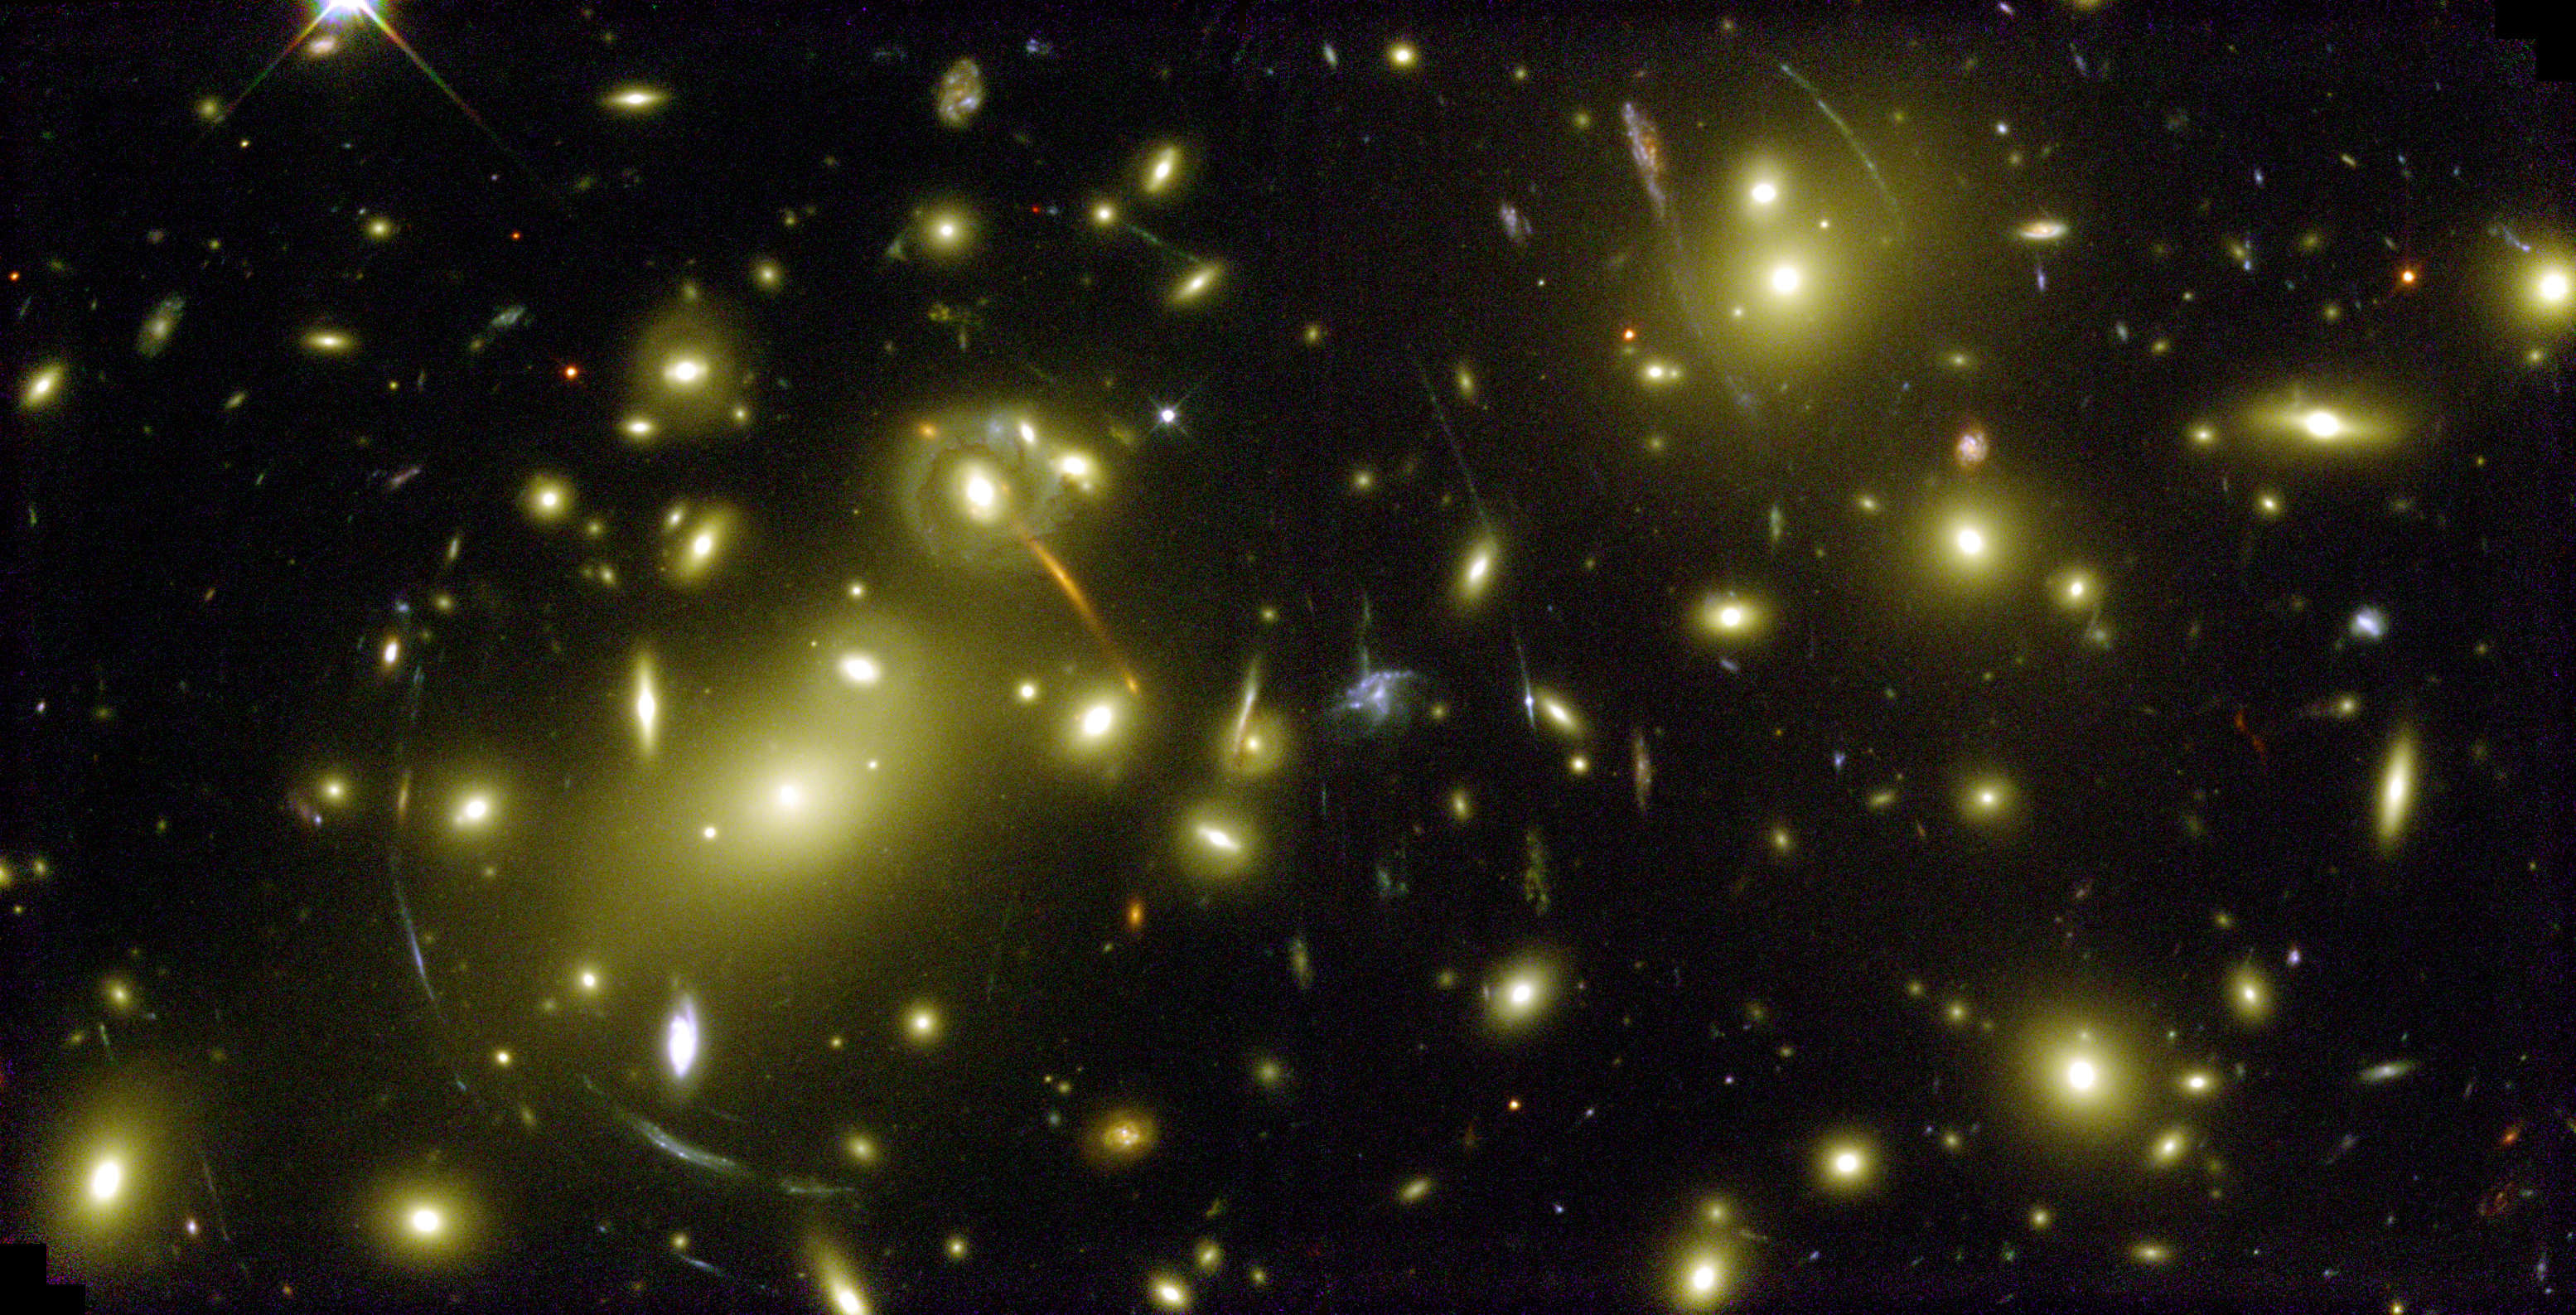
\includegraphics[width=\textwidth]{cluster/images/HSTCI_PR00-08}
  \caption{Galaxiencluster (Abell 2218; NASA, ERO Team)
    \cite{wiki:abell}}
  \label{fig:abell}
\end{figure}

\section{``Normale'' Linse}
\rhead{Normale Linse}
Zuerst einmal ein Rückblick wie eine ``normale'' Linse funktioniert.
Eine ``normale'' Linse nutzt die Brechung zwischen dem Linsenmaterial
und seiner Umgebung aus.  Durch diese Brechung kommt es zu einer
Winkeländerung des Lichtstrahls.  Bei homogenen Materialien mit
bekannten Brechungsindizes kann folgende Formel aus der geometrischen
Optik verwendet werden:

\begin{equation}
  \frac{\sin \varepsilon_1}{\sin \varepsilon_2} = \frac{n_2}{n_1}.
\end{equation}

Darin kommen die Winkel zur Oberflächennormalen im Sinus-Bruch
und die beiden Brechungsindizes vor.  Der
Brechungsindex eines Mediums \(n\), ergibt sich aus der
Lichtgeschwindigkeit im Vakuum \(c\) geteilt durch die
Lichtgeschwindigkeit \(u\) im Medium:

\begin{equation}
  n = \frac{c}{u}.
\end{equation}
\index{Brechungsindex}


\subsection{Prinzip von Huygens}
\rhead{Prinzip von Huygens}
\index{Huygens!Prinzip von}
Wie sich das Licht ausbreitet lässt sich anschaulich mit dem Prinzip
von Huygens aufzeigen.  In der Abbildung \ref{fig:huygens1} ist die
Lichtwellenausbreitung in einem homogenen Medium gezeigt.  Die
Lichtwelle (rote Linie unten) ist nach einem Zeitschritt
(\(\Delta t\)) an der mittleren Position zu finden.  Nach einem
weiteren \(\Delta t\) ist die Lichtwelle an der Position der obersten
roten Linie.  In der Abbildung bewegt sich die Lichtwelle von unten
nach oben.  Weil es sich um ein homogenes Material handelt, sind die
Abstände zwischen den Lichtwellen parallel und immer im gleichen
Abstand.  Das Prinzip von Huygens sagt nun, dass man von jedem Punkt
aus auf einer Lichtwelle (rote Linie), einen Halbkreis in
Ausbreitungsrichtung einzeichnen kann.  Der Halbkreis ist die Distanz,
welche das Licht nach \(\Delta t\) zurückgelegt hat.  Legt man nun
eine Umhüllende um die Halbkreise, erhält man die Position der
Lichtwelle zum neuen Zeitpunkt.

\begin{figure}
  \centering
  %
% Brechung nach dem Prinzip von Huygens


\begin{tikzpicture}

  
  % Delta t
  \foreach \y in {-1,0,1}
    \draw [very thick, color=red] (0,\y) -- (6,\y);

  \foreach \x in {1,2,3,4,5}
    \draw [black, fill=white] (\x,0) circle (.6mm);

  \foreach \x in {1,2,3,4,5}
    \draw [blue] (\x,0) ++ (0,1) arc (90:160:1cm)
                 (\x,0) ++ (0,1) arc (90:20:1cm);

  \draw [very thick, color=red, ->, >=stealth] (-.5,-.5) -- (-.5,0.5);
  \draw [very thick, color=red, ->, >=stealth] (6.5,-.5) -- (6.5,0.5);


\end{tikzpicture}
  \caption{Lichtwellen Ausbreitung nach dem Prinzip von Huygens.}
  \label{fig:huygens1}
\end{figure}

Hat man zwei verschiedenen homogene Materialien, kommt es zur
Brechung, welche auch mit dem Prinzip von Huygens gezeigt werden kann.
In der Abbildung \ref{fig:huygens2} kommt die Lichtwelle von oben
links.  Zum Zeitpunkt in dem die Lichtwelle die beiden Punkte \(A\)
und \(B\) bildet, berührt die Lichtwelle im Punkt \(A\) den
Materialübergang.  Zeichnet man nun die ``Bewegungs-Halbkreise'' ein,
so ist der Halbkreis ausgehend von \(B\) grösser als von \(A\).  Der
Grund dafür ist die höhere Lichtgeschwindigkeit im weissen Medium als
im blauen Medium.  Legt man von \(D\) aus die Tangente an den von
\(A\) ausgehenden Halbkreis, erhält man die Lichtwelle nach
\(\Delta t\).  Es ist gut sichtbar, dass die Lichtwelle
\(\overline{CD}\) gebrochen wurde und nicht parallel zu
\(\overline{AB}\) liegt.

\begin{figure}
  \centering
  \input{cluster/tikz/huygens2.tikz}
  \caption{Brechung nach dem Prinzip von Huygens.}
  \label{fig:huygens2}
\end{figure}

Im Fall der Gravitationslinse gibt es im Weltall natürlich keine starr
begrenzte homogene Bereiche.  Besser zum Vergleich geeignet ist die
Abbildung \ref{fig:huygens3} mit einem inhomogenen Material.  Durch
die tiefere Lichtgeschwindigkeit im blauen Material ist der Abstand
zwischen den Lichtwellen kleiner als im weissen Material, somit biegt
sich der Lichtstrahl.

Da die Lichtgeschwindigkeit in einem Gebiet mit hoher Gravitation
langsamer vergeht, biegen sich Lichtstrahlen in Richtung massen
schwere Objekte.  (Zum Beispiel könnte im Zentrum der blauen Fläche
ein Stern stehen.  Licht, welches nahe dem Stern vorbeigeht, wird in
Richtung des Sterns abgelenkt.)

\begin{figure}
  \centering
  %
% Brechung nach dem Prinzip von Huygens


\begin{tikzpicture}
  [every label/.style={color=black}]

  
  %

  \shade [inner color=blue!50!white, outer color=white] (-.6,0.55) circle (1.5cm);

  \coordinate (A) at (0,0);
  \coordinate (B) at (3,0);
  \draw [very thick, color=red] (A) -- (B);

  \path (B) ++ (97:1cm) coordinate (Bs);
  \path (Bs) ++ ($ (A)!1!187:(B) $) coordinate (As);
  \draw [very thick, color=red] (As) -- (Bs);

  \path (Bs) ++ (104:1cm) coordinate (Bss);
  \path (Bss) ++ ($ (A)!1!194:(B) $) coordinate (Ass);
  \draw [very thick, color=red] (Ass) -- (Bss);

  \draw [very thick, color=red] (A) ++ (0,-1) --++ ($ (B)-(A) $);
  \draw [very thick, color=red] (Bss) ++ (104:1cm) --++ ($ (A)!1!194:(B) $);

  
  % \fill [fill=blue!15!white] (0,0) rectangle (6,-2);
  % \draw [thick] (0,0) -- (6,0);
  % \coordinate[label=below left:$A$] (A) at (3,0);
  % \path (A) ++ (2,0) coordinate[label=below right:$D$] (D);

  % \draw [very thick, color=red, -<, >=stealth] (A) --++ (150:2.5) node(ray1Start){};
  % \path [name path=rayStart] (ray1Start.center) --++ (60:2.5);
  % \path [name path=ray2] (A) ++ (2,0) --++ (150:6);
  % \draw [very thick, color=red, name intersections={of=rayStart and ray2,
  %   by=ray2Start}, -<, >=stealth] (A) ++ (2,0) -- (ray2Start);

  % \path (ray2Start) ++ (-30:2.5) coordinate[label=above:$B$] (B);
  % \draw [color=red] (A) -- (B);


  % \draw [thick, color=blue] (A) ++ (.8,0) arc (0:-180:.8cm);
  % \draw [thick, color=blue]
  %   let \p1 = ($(B)-(D)$)
  %   in (B) ++ (-30:{veclen(\x1,\y1)}) arc (-30:140:{veclen(\x1,\y1)})
  %      (B) ++ (150:{veclen(\x1,\y1)}) coordinate (Bs)
  %      (A) ++ (150:{veclen(\x1,\y1)}) coordinate (As);

  % \draw [color=red] (As) -- (Bs);

  % \node [circle] (circleSmall) at (A) [minimum size=2*.8cm,
  %   inner sep=0]{};
  % \draw [color=red] (D) -- (tangent cs:node=circleSmall, point={(D)},
  %   solution=2) coordinate[label=below left:$C$] (C);


  % \path (C) ++ ($ (C)-(A) $) coordinate (Cs);
  % \path (D) ++ ($ (C)-(A) $) coordinate (Ds);
  % \draw [very thick, color=red, ->, >=stealth] (A) -- (C) -- ($ (C)!1.4!(Cs) $);
  % \draw [very thick, color=red, ->, >=stealth] (D) -- ($ (D)!1.4!(Ds) $);
  % \draw [color=red] (Cs) -- (Ds);

  % \foreach \point in {A,B,C,D}
  %   \draw [black, fill=white] (\point) circle (.6mm);


\end{tikzpicture}
  \caption{Brechung nach dem Prinzip von Huygens in einem inhomogen
    Material.}
  \label{fig:huygens3}
\end{figure}


\section{Gravitationslinse}
\rhead{Gravitationslinse}
\subsection{Einfluss der Gravitation auf die Zeit}
\rhead{Einfluss der Gravitation auf die Zeit}
Als Start wird die Formel \eqref{skript:kruemmung:raumzeitabstand}
\begin{equation*}
  s^2 = -c^2 (t_1-t_2)^2 + (x_1-x_2)^2 + (y_1-y_2)^2 + (z_1-z_2)^2
\end{equation*}
aus dem Abschnitt über den Lichtkegel genommen.

Die Gravitationslinse beugt Lichtwellen, somit ist \(s^2=0\), da sich
die Wirkung mit Lichtgeschwindigkeit ausbreitet.  Wird zur
Vereinfachung \(c=1\) gesetzt, ergibt sich:
\begin{equation*}
  0 = -(t_1-t_2)^2 + (x_1-x_2)^2 + (y_1-y_2)^2 + (z_1-z_2)^2
\end{equation*}
oder anders geschrieben
\begin{equation*}
  0 = -dt^2 + dx^2 + dy^2 + dz^2.
\end{equation*}

Die Lichtwellen bewegen sich in minimalen Wegen, was den Geodäten
entspricht.  Die Lichtablenkung an Sternen und Galaxien befindet sich
im Bereich von schwachen Gravitationsfeldern.  Zu diesen wurden die
\(g_{\mu\nu}\):
\begin{align*}
  g_{00} &= -1 -\frac{2\varphi}{c^2} &g_{kk} &= 1,\quad k=1,2,3
\end{align*}
bereits berechnet (Formel \ref{skript:gravitation:naeherung}).
Das Gravitationspotential \(\varphi\) ist für eine Punktmasse:
\begin{equation*}
  \varphi = -\frac{KM}{r}
\end{equation*}
\(M\) ist die Punktmasse, \(K\) die Gravitationskonstante
(oft als \(G\) bezeichnet) und \(r\) der Abstand zur Punktmasse.
Setzt man dies nun zusammen, erhält man folgende \(g_{\mu\nu}\):
\begin{align*}
  g_{00} &= -1 +\frac{2KM}{rc^2} &g_{kk} &= 1,\quad k=1,2,3.
\end{align*}
Für grosse Abstände \(r\) wird \(g_{00}=-1\).  Was gleich der normalen
Minkowski-Metrik ist.

\begin{beispiel}
  In folgendem soll die Zeitveränderung für Werte unserer Sonne
  berechnet werden.  Die Werte sind:
  \begin{align*}
    K &= \SI{6.67e-11}{\meter\cubed\per\kilogram\per\second\squared}
    &M &= \SI{1.99e30}{\kilogram}
    &c &= \SI{2.99e8}{\meter\per\second}.
  \end{align*}
  Die Zeitveränderung wird nur vom zweiten Teil von \(g_{00}\)
  bestimmt, wobei man erhält:
  \begin{align*}
    \tilde{t} &= \frac{2KM}{rc^2}
    &\left[\tilde{t}\right] &=
                              \si{\meter\cubed\per\kilogram\per\second\squared}
                              \cdot \si{\kilogram}
                              \cdot \si{\per\meter}
                              \cdot \si{\per\meter\squared\second\squared}
                              = 1.
  \end{align*}
  Einen Graphen mit den Werten von \(1\) bis \(0.05\) für
  \(\tilde{t}\) mit dem Abstand \(r\) kann in der Abbildung
  \ref{fig:bsp1} gefunden werden.  Ein \(\tilde{t}\) von \(0.25\)
  entspricht einer Verlangsamung von Wasser.  Je näher bei
  \(\tilde{t}=1\) desto langsamer bewegt sich das Licht, da
  \(g_{00} \rightarrow 0\) wird.  Es ist zu beachten, dass das
  geplotete maximale \(r\) von \SI{60000}{\meter} immer noch innerhalb
  der Sonne ist, da der Sonnenradius \SI{\approx 700e6}{\meter}
  entspricht.
  \begin{figure}
    \centering
    

\begin{tikzpicture}[scale = 1.7]
    \datavisualization[scientific axes = clean,
                     y axis = {grid,
                               label=\(\tilde{t}\) von \(1\) bis \(0.05\),
                               min value = 0,
                               max value = 1},
                     x axis = {grid,
                               label=\(r\) in \si{\meter},
                               min value = 0,
                               max value = 60000},
                     visualize as smooth line/.list={ch1},
                     style sheet=vary hue,
                     %style sheet=vary dashing,
                     %ch1={label in legend={text=Mittenkavität}},
                     ]
                    
  data [set=ch1,headline={x, y}, read from file=cluster/source/bsp1.csv];
\end{tikzpicture}
    \caption{\(\tilde{t}\) von \(1\) bis \(0.05\)}
    \label{fig:bsp1}
  \end{figure}
\end{beispiel}

Im obigen Beispiel ist gut ersichtlich, wie schnell der Einfluss der
Gravitation abnimmt.  Eine Linse mit dieser Eigenschaft müsse so
geformt sein, wie ein Weinglasboden.  In der Abbildung
\ref{fig:ModelGravLinse} sind drei Beispielkonstellationen zu sehen.
Ist der Weinglasboden in einer Linie mit der Kerze (unten links)
erhält man ein Einsteinring ähnliches Gebilde.  Bei einem gekippten
Boden (oben rechts) erhält man beinahe ein Einsteinkreuz.  Und unten
rechts sieht man ein Beispiel was passiert, wenn die Linse und die
Quelle nicht in einer Linie stehen (wie im Cluster Bild
\ref{fig:abell}).

\begin{figure}
  \centering
  \includegraphics[width=\textwidth]{cluster/images/model_grav_lens}
  \caption{Model einer Gravitationslinse (Boden eines Weinglases)
    \cite{standford:ModelGravLens}}
  \label{fig:ModelGravLinse}
\end{figure}

\subsection{Euler-Lagrange}
\rhead{Euler-Lagrange}
\index{Euler-Lagrange-Gleichungen}
Um die Lichtablenkung zu berechnen, benötigt man den Weg des Lichts
und nicht nur wie stark die Lichtgeschwindigkeit abgebremst wird.  Das
Licht nimmt den Weg mit der kürzesten Laufzeit.  Aus der Physik kennt
man, dass die Zeit gleich der Strecke durch die Geschwindigkeit ist:
\begin{equation*}
  t = \frac{s}{v}.
\end{equation*}

Für den Weg des Lichts muss man somit jedes Wegstück mit seiner
Geschwindigkeit dividieren und all diese Stückchen zusammen addieren.
Das Licht nimmt nun den Weg, in welchem es die kürzeste Laufzeit hat.
Um eine Strecke zu minimieren, kann man Euler-Lagrange verwenden,
welche ein Integral der Form
\begin{equation*}
  I = \int\limits_{t_0}^{t_1}\! F\bigl(x^{\alpha}(t), \dot{x}^{\alpha}(t),t\bigr)d t
\end{equation*}
benötigt.  Das Integral soll die Zeit minimieren, somit muss es einen
Weg geteilt durch eine Geschwindigkeit im Integral geben.  Eine
Möglichkeit ist folgendes Integral:
\begin{equation}
  I = \int\! \sqrt{\dot{x}(l)^2+\dot{y}(l)^2+\dot{z}(l)^2} \cdot
  \frac{n\bigl(x(l),y(l),z(l)\bigr)}{c} d l.
\end{equation}

Der Wert unter der Wurzel entspricht dem Wegstück während eines
Integrationsschritts.  Die Division entspricht eins durch die
Geschwindigkeit.  Somit erhält man im Integral eine Zeit, welche über
den gesamten Weg integriert der Wegzeit des Lichts entspricht.  Da die
Lichtgeschwindigkeit \(c\) unabhängig von der Position ist, kann man
den Bruch vor das Integral nehmen:
\begin{equation}
  I = \frac{1}{c}\int\! \sqrt{\dot{x}(l)^2+\dot{y}(l)^2+\dot{z}(l)^2}
  \cdot n\bigl(x(l),y(l),z(l)\bigr) d l.
\end{equation}
Des Weiteren benötigt man für Euler-Lagrange nur den Teil im Integral:
\begin{equation}
  L = \sqrt{\dot{x}(l)^2+\dot{y}(l)^2+\dot{z}(l)^2}
  \cdot n\bigl(x(l),y(l),z(l)\bigr).
\end{equation}
Da die Wurzel die folgenden Rechenschritte verkompliziert, wird sie
quadriert, was das Extremum nicht verändert.  Dieser Schritt wurde
bereits im Abschnitt
\ref{skript:geodaeten:subsection:Parametrisierung} angewendet.  Weiter
wird die Abhängigkeit von \(l\) nicht mehr geschrieben, was es
natürlich bleibt:
\begin{equation}
  F = L^2 = (\dot{x}^2+\dot{y}^2+\dot{z}^2)n^2.
\end{equation}

Für Euler-Lagrange muss man nun dieses \(F\) ableiten, im folgenden
nur mit \(x\) gezeigt:
\begin{equation}
  \label{eq:cluster:euler}
  0 = \frac{\partial F}{\partial x} - \frac{d}{d l} \frac{\partial
    F}{\partial \dot{x}}.
\end{equation}
Die Ableitungen sind
\begin{align*}
  \frac{\partial F}{\partial x} &= (\dot{x}^2+\dot{y}^2+\dot{z}^2) 2n
                                  \frac{\partial n}{\partial x}\\
  \frac{\partial F}{\partial\dot{x}} &= 2\dot{x}n^2\\
  \frac{d}{d l}\frac{\partial F}{\partial\dot{x}} &= 2\ddot{x}n^2 + 4\dot{x}n
                                \left(\frac{\partial n}{\partial x}\dot{x} +
                                \frac{\partial n}{\partial y}\dot{y} +
                                \frac{\partial n}{\partial z}\dot{z} \right).
\end{align*}
Setzt man die obigen Berechnungen in \ref{eq:cluster:euler} ein und
löst diese Formel nach \(\ddot{x}\) auf, erhält man:
\begin{equation}
  \ddot{x} = (-\dot{x}^2+\dot{y}^2+\dot{z}^2)
  \frac{1}{n}\frac{\partial n}{\partial x} -
  2\dot{x}\dot{y} \frac{1}{n}\frac{\partial n}{\partial y} -
  2\dot{x}\dot{z} \frac{1}{n}\frac{\partial n}{\partial z}.
\end{equation}
Mit der Hilfe der logarithmischen Differentiation
\begin{equation*}
  \frac{1}{n} \frac{\partial n}{\partial x} = \frac{\partial \ln
    n}{\partial x}
\end{equation*}
kann man die Formel weiter vereinfachen:
\begin{equation}
  \ddot{x} = (-\dot{x}^2+\dot{y}^2+\dot{z}^2) \frac{\partial \ln
    n}{\partial x} - 2\dot{x}\dot{y} \frac{\partial \ln n}{\partial y}
  - 2\dot{x}\dot{z} \frac{\partial \ln n}{\partial z}.
\end{equation}
Normalerweise ist ein Logarithmus nicht der einfachste Ansatz.  Die
Vereinfachung entsteht durch die spezielle Form von \(n\)
\begin{equation*}
  n \approx 1-\frac{2\varphi}{c^2}
\end{equation*}
und weil
\begin{equation*}
  \frac{\varphi}{c^2} \ll 1
\end{equation*}
ergibt sich
\begin{equation*}
  \ln n \approx -\frac{2\varphi}{c^2}.
\end{equation*}

Somit muss man nun keine partielle Ableitung von \(\ln n\), sondern von
\(-\frac{2\varphi}{c^2}\) durchführen (d.h. man braucht
\(\nabla\varphi=\) Gravitationskraft).  In einem Beispiel soll dies in
2D gezeigt werden.

\begin{beispiel}
  Im Folgenden wird die Lichtablenkung in einem zwei dimensionalen
  Raum numerisch berechnet.  Als \(\varphi\) wird eine Punktquelle
  verwendet:
  \begin{equation*}
    \varphi = -\frac{KM}{r}.
  \end{equation*}
  Wobei
  \begin{equation*}
    r = \sqrt{(x-x_L)^2+(y-y_L)^2}
  \end{equation*}
  der Abstand zwischen dem aktuellen Punkt und der Linse ist.

  Berechnet man mit Hilfe von Maxima Euler-Lagrange nach den beiden
  Koordinatenachsen, erhält man:
  \begin{align*}
    \ddot{x} &= -\frac{2(-\dot{x}^2+\dot{y}^2)(x-x_L)KM}
               {c^2\sqrt{(x-x_L)^2+y^2}\,^3}+
               \frac{4\dot{x}y\dot{y}KM}{c^2\sqrt{(x-x_L)^2+y^2}\,^3}\\
    \ddot{y} &= +\frac{4\dot{x}\dot{y}(x-x_L)KM}{c^2\sqrt{(x-x_L)^2+y^2}\,^3}
               - \frac{2(\dot{x}^2-\dot{y}^2)yKM}
               {c^2\sqrt{(x-x_L)^2+y^2}\,^3}.
  \end{align*}
  In diesem Beispiel befindet sich die Gravitationslinse auf \(x=0\),
  somit vereinfacht sich \(y-y_L\) zu \(y\).  Die soeben erhaltenen
  Formeln kann man in dieser Form noch nicht verwenden.  Man hat ein
  Differentialgleichungssystem zweiter Ordnung.  Was von geläufigen
  Computer Algorithmen nicht gelöst werden kann, da sie ein DGL-System
  erster Ordnung benötigen.

  Mit Substitution kann man eine Differentialgleichung zweiter Ordnung
  in ein DGL-System erster Ordnung überführen.  Macht man diese
  Substitution mit beiden Formeln, erhält man ein Gleichungssystem
  erster Ordnung, welche beide Formeln enthält.  Wählt man folgende
  Substitutionen
  \begin{align*}
    x_1 &= x &x_2 &= \dot{x} &x_3 &= y &x_4 &= \dot{y}
  \end{align*}
  kann man die beiden Formeln in eine brauchbare Form bringen.  Die
  gängigen Algorithmen fordern die Ableitungen von \(x_k\) als
  Parametern:
  \begin{align*}
    \dot{x}_1 &= x_2\\
    \dot{x}_2 &= -\frac{2\left(-x_2^2+x_4^2\right)\bigl(x_1-x_L\bigr)KM}
                {c^2\sqrt{\bigl(x_1-x_L\bigr)^2+x_3^2}\,^3}
                + \frac{4 x_2x_3x_4 KM}
                {c^2\sqrt{\bigl(x_1-x_L\bigr)^2+x_3^2}\,^3}\\
    \dot{x}_3 &= x_4\\
    \dot{x}_4 &= +\frac{4x_2x_4\bigl(x_1-x_L\bigr)KM}
                {c^2\sqrt{\bigl(x_1-x_L\bigr)^2+x_3^2}\,^3}
                - \frac{2 \left(x_2^2-x_4^2\right) x_3 KM}
                {c^2\sqrt{\bigl(x_1-x_L\bigr)^2+x_3^2}\,^3}.
  \end{align*}

  In Octave wird \(x_k\) zu \texttt{x(k)}, was zu folgendem Code
  führt:
  \lstinputlisting[style=Octave]{cluster/source/dglSubCode.m}

  Setzt Man nun die Werte
  \begin{align*}
    x_L &\approx \SI{150e6}{\kilo\meter} &M &\approx
                                              \SI{2e30}{\kilogram}
    &R &\approx \SI{700e3}{\kilo\meter}
  \end{align*}
  der Sonne ein,
  erhält man eine Winkeländerung von \(\approx \SI{1.75}{''}\),
  vergleicht man dies mit dem Wert aus der Literatur von
  \(\SI{1.75}{''}\) (\cite{misner1973gravitation} S.446), scheint
  dieses Vorgehen ziemlich adäquat.

  Im Graphen \ref{fig:lichtablenkungSonne} ist der numerisch
  berechnete Lichtweg dargestellt.  Der Beobachter ist im Punkt (0,0)
  und die Sonne im Punkt (\SI{1.5e11}{\meter},0).  Der Lichtpfad
  startet von der Erde aus so, dass man direkt am Sonnenradius
  vorbeischaut.  Da die Ablenkung nur \SI{1.75}{''} ist, sieht der Lichtweg
  von Auge betrachtet wie eine gerade Strecke aus.  (Eine Bogensekunde
  ist ein 3600stel eines Grades.)

  Nimmt man zur Berechnung eine schwerere Sonne an, ist die
  Lichtablenkung auch von Auge gut zu sehen.  In der Abbildung
  \ref{fig:lichtablenkung300Sonne} ist die Sonne 300 mal schwerer (bei
  gleichem Radius) und in \ref{fig:lichtablenkung600Sonne} sogar 600
  mal mehr.

  \begin{figure}
    \centering
    \begin{tikzpicture}[scale = 1.7]
      \datavisualization[scientific axes = clean,
                         y axis = {grid,
                                   label=\(y\) in \si{\meter},
                                   min value = 0,
                                   max value = 1.5e9},
                         x axis = {grid,
                                   label=\(x\) in \si{\meter},
                                   min value = 0,
                                   max value = 3e11},
                         visualize as smooth line/.list={ch1},
                         % ch1={style=very thick},
                         style sheet=vary hue,
                         % style sheet=vary dashing,
                         % ch1={label in legend={text=Mittenkavität}},
                        ]
                    
      data [set=ch1,headline={x, y}, read from file=cluster/source/lichtablenkungSonne.csv];
    \end{tikzpicture}
    \caption{Lichtablenkung an der Sonne}
    \label{fig:lichtablenkungSonne}
  \end{figure}
  
  \begin{figure}
    \centering
    \begin{tikzpicture}[scale = 1.7]
      \datavisualization[scientific axes = clean,
                         y axis = {grid,
                                   label=\(y\) in \si{\meter},
                                   min value = 0,
                                   max value = 1.5e9},
                         x axis = {grid,
                                   label=\(x\) in \si{\meter},
                                   min value = 0,
                                   max value = 3e11},
                         visualize as smooth line/.list={ch1},
                         % ch1={style=very thick},
                         style sheet=vary hue,
                         % style sheet=vary dashing,
                         % ch1={label in legend={text=Mittenkavität}},
                        ]
                    
      data [set=ch1,headline={x, y}, read from file=cluster/source/lichtablenkung300Sonne.csv];
    \end{tikzpicture}
    \caption{Lichtablenkung an 300 Sonnenmassen}
    \label{fig:lichtablenkung300Sonne}
  \end{figure}
  
  \begin{figure}
    \centering
    \begin{tikzpicture}[scale = 1.7]
      \datavisualization[scientific axes = clean,
                         y axis = {grid,
                                   label=\(y\) in \si{\meter},
                                   min value = 0,
                                   max value = 1.5e9},
                         x axis = {grid,
                                   label=\(x\) in \si{\meter},
                                   min value = 0,
                                   max value = 3e11},
                         visualize as smooth line/.list={ch1},
                         % ch1={style=very thick},
                         style sheet=vary hue,
                         % style sheet=vary dashing,
                         % ch1={label in legend={text=Mittenkavität}},
                        ]
                    
      data [set=ch1,headline={x, y}, read from file=cluster/source/lichtablenkung600Sonne.csv];
    \end{tikzpicture}
    \caption{Lichtablenkung an 600 Sonnenmassen}
    \label{fig:lichtablenkung600Sonne}
  \end{figure}
\end{beispiel}

Im vorherigen Beispiel sieht man gut, dass die Lichtstrahlen bis
praktisch zur Sonne eine Gerade darstellen, dann abgebogen werden und
wieder in einer Gerade weiterfliegen.  Stellt man nur diese Ablenkung
dar (\ref{fig:lichtablenkung600SonneZoom}) ist das noch besser
sichtbar.

\begin{figure}
  \centering
  \begin{tikzpicture}[scale = 1.7]
    \datavisualization[scientific axes = clean,
                       y axis = {grid,
                                 label=\(y\) in \si{\meter},
                                 min value = 6.5e8,
                                 max value = 7e8},
                       x axis = {grid,
                                 label=\(x\) in \si{\meter},
                                 min value = 1.4e11,
                                 max value = 1.6e11},
                       visualize as smooth line/.list={ch1},
                       % ch1={style=very thick},
                       style sheet=vary hue,
                       % style sheet=vary dashing,
                       % ch1={label in legend={text=Mittenkavität}},
                      ]
                    
    data [set=ch1,headline={x, y}, read from file=cluster/source/zoomLichtablenkung600Sonne.csv];
  \end{tikzpicture}
  \caption{Lichtablenkung an 600 Sonnenmassen (Zoom)}
  \label{fig:lichtablenkung600SonneZoom}
\end{figure}

Das Verhalten, dass über eine lange Strecke nichts passiert, erschwert
die nummerische Berechnung.  Die Algorithmen ode23 und ode45 in Octave
waren nicht in der Lage den Weg zu berechnen.  Hingegen konnte die
Lichtablenkung im Beispiel oben mit ode23s aus Octave berechnet
werden.  Dieser Algorithmus ist fähig steife Probleme zu berechnen.
Solche Probleme nennt man steif, wenn eine tiefe Frequenz von einer
hohen Frequenz überlagert wird.  Im weiteren Sinn ist dieses Problem
steif, da zwischen Beobachter, Gravitationslinse und Quelle sehr
grosse Abstände vorhanden sind, in denen nichts passiert.  Zum Lösen
berechnet ode23s auf der gesamten vorgegebenen Strecke Punkte.  Für
Sonnenabstände ist dies noch gut berechenbar, für Galaxienabstände
jedoch nicht.

\subsection{Bildverzerrung}
\rhead{Bildverzerrung}
Möchte man nun ein Bild der Lichtablenkung erzeugen, muss man für
jedes Pixel den Lichtweg simuliert.  Wenn man den einfachsten Fall der
Punktquelle beibehält, kann man die Symmetrie ausnützen und muss somit
nur ein Achtel der Pixelauflösung berechnen.

Für die Simulation wurde wieder der Abstand von der Erde zur Sonne
verwendet.  Um die Lichtablenkung noch zu verstärken, wurde die
tausendfache Sonnenmasse bei gleichem Radius angenommen.  Der
Pixelabstand in der Sonnenebene liegt bei \SI{10e6}{\meter}.  Das
Hintergrundbild, die Andromeda Galaxie aus Abbildung \ref{fig:m31},
ist in rund 6.8 fachem Sonnenabstand von der Erde aus platziert.  Der
Pixelabstand wurde gleich gewählt.

\begin{figure}
  \centering
  \includegraphics[width=\textwidth]{cluster/images/m31_comolli_2193}
  \caption{Andromeda Galaxie M31 \cite{nasa:andromedaM31}}
  \label{fig:m31}
\end{figure}

In der Abbildung \ref{fig:einsteinringSim} sieht man, wie das Zentrum
der Galaxie zu einem Ring verzogen wird.  Das schwarze Zentrum in der
Abbildung ist die Position der ``Sonne''.  Die Abbildung hat eine
Auflösung von \(300\times300\) Pixel und benötigte gut eineinhalb Tage
Berechnungszeit bei vier Kernen mit Hyper-Threading.

\begin{figure}
  \centering
  \includegraphics[width=.6\textwidth]{cluster/images/einsteinring}
  \caption{Bildverzerrung durch 1000 Sonnenmassen}
  \label{fig:einsteinringSim}
\end{figure}

\printbibliography[heading=subbibliography]
\end{refsection}


\chapter{Lichtablenkung an einem Galaxiencluster\label{chapter:thema}}
\lhead{Lichtablenkung an einem Galaxiencluster}
\begin{refsection}
\chapterauthor{Pascal Stump}

\section{Einleitung}
\rhead{Einleitung}
Wenn ein sehr massereiches Objekt zwischen einem Betrachter und einer
Lichtquelle platziert ist, tritt ein Gravitationslinseneffekt auf.  In
der Abbildung \ref{fig:lrg3-757} sieht man ein Beispiel, bei welchem
die Vordergrund-Galaxie (gelb/orange) praktisch in einer Linie zur
Hintergrund-Galaxie (blau) steht.  Durch die beinahe optimale
Ausrichtung in einer Linie wird die Hintergrund-Galaxie zu einem
Kreis verzerrt.  Der dabei entstehende Kreis wird auch Einsteinring
genannt.

Wenn die Vordergrund-Galaxie nicht rotationssymmetrisch ist, kann die
Hintergrund-Galaxie zu einzelnen Punkten verzerrt werden, so zu sehen
in der Abbildung \ref{fig:einsteinkreuz}.  Dabei ist die
Vordergrund-Galaxie wieder in der Mitte zu finden und die vier
umliegenden Punkte sind die verzerrte Hintergrund-Galaxie.

Ein drittes Beispiel des Gravitationslinseneffekts ist in Abbildung
\ref{fig:abell} zu finden.  Dabei ist nicht nur eine Galaxie als Linse
zuständig, sondern ein Galaxiencluster.  Die Vordergrund-Galaxien ist
wiederum die gelb, orange farbigen Galaxien.  Man sieht schön, dass
die Hintergrund-Galaxien zu Streifen verzogen werden und nicht mehr zu
einem ganzen Kreis, da die Ausrichtungen zueinander nicht optimal
sind.

\begin{figure}
  \centering
  \includegraphics[width=\textwidth]{cluster/images/LRG_3-757}
  \caption{Einsteinring (LRG 3-757; ESA/Hubble \& NASA)
    \cite{nasa:einsteinring, wiki:einsteinring}}
  \label{fig:lrg3-757}
\end{figure}

\begin{figure}
  \centering
  \includegraphics[width=.7\textwidth]{cluster/images/Einstein_cross}
  \caption{Einsteinkreuz (G2237+0305; NASA, ESA \& STScl)
    \cite{wiki:einsteinkreuz}}
  \label{fig:einsteinkreuz}
\end{figure}

\begin{figure}
  \centering
  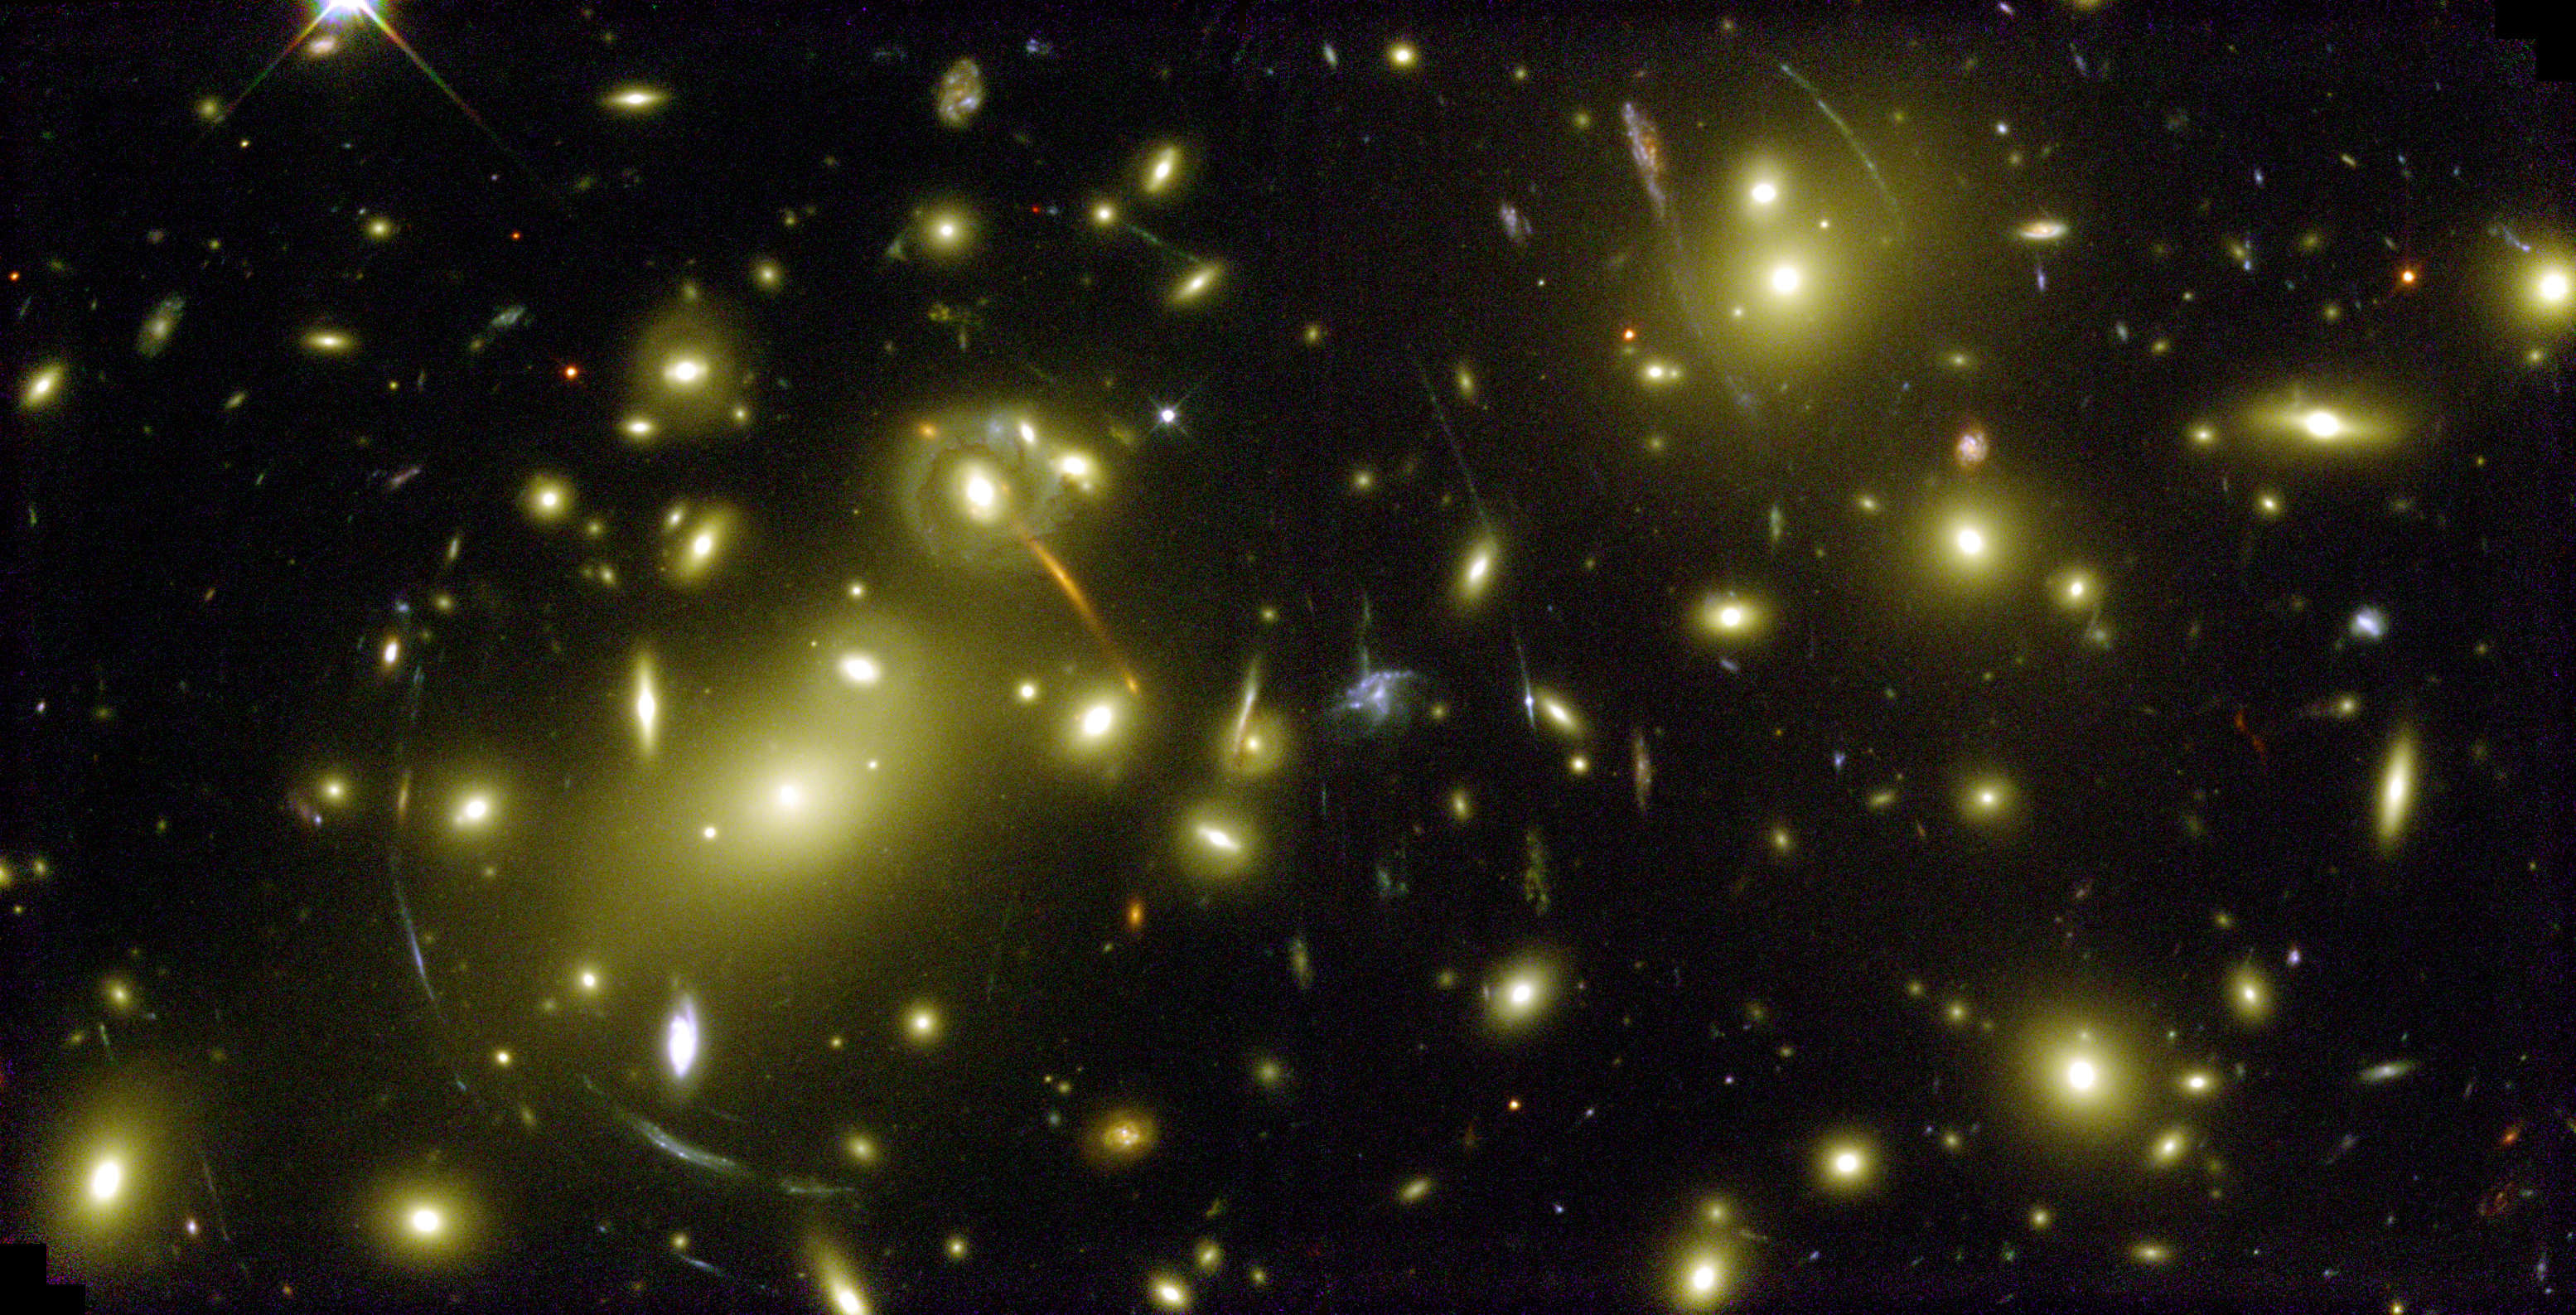
\includegraphics[width=\textwidth]{cluster/images/HSTCI_PR00-08}
  \caption{Galaxiencluster (Abell 2218; NASA, ERO Team)
    \cite{wiki:abell}}
  \label{fig:abell}
\end{figure}

\section{``Normale'' Linse}
\rhead{Normale Linse}
Zuerst einmal ein Rückblick wie eine ``normale'' Linse funktioniert.
Eine ``normale'' Linse nutzt die Brechung zwischen dem Linsenmaterial
und seiner Umgebung aus.  Durch diese Brechung kommt es zu einer
Winkeländerung des Lichtstrahls.  Bei homogenen Materialien mit
bekannten Brechungsindizes kann folgende Formel aus der geometrischen
Optik verwendet werden:

\begin{equation}
  \frac{\sin \varepsilon_1}{\sin \varepsilon_2} = \frac{n_2}{n_1}.
\end{equation}

Darin kommen die Winkel zur Oberflächennormalen im Sinus-Bruch
und die beiden Brechungsindizes vor.  Der
Brechungsindex eines Mediums \(n\), ergibt sich aus der
Lichtgeschwindigkeit im Vakuum \(c\) geteilt durch die
Lichtgeschwindigkeit \(u\) im Medium:

\begin{equation}
  n = \frac{c}{u}.
\end{equation}
\index{Brechungsindex}


\subsection{Prinzip von Huygens}
\rhead{Prinzip von Huygens}
\index{Huygens!Prinzip von}
Wie sich das Licht ausbreitet lässt sich anschaulich mit dem Prinzip
von Huygens aufzeigen.  In der Abbildung \ref{fig:huygens1} ist die
Lichtwellenausbreitung in einem homogenen Medium gezeigt.  Die
Lichtwelle (rote Linie unten) ist nach einem Zeitschritt
(\(\Delta t\)) an der mittleren Position zu finden.  Nach einem
weiteren \(\Delta t\) ist die Lichtwelle an der Position der obersten
roten Linie.  In der Abbildung bewegt sich die Lichtwelle von unten
nach oben.  Weil es sich um ein homogenes Material handelt, sind die
Abstände zwischen den Lichtwellen parallel und immer im gleichen
Abstand.  Das Prinzip von Huygens sagt nun, dass man von jedem Punkt
aus auf einer Lichtwelle (rote Linie), einen Halbkreis in
Ausbreitungsrichtung einzeichnen kann.  Der Halbkreis ist die Distanz,
welche das Licht nach \(\Delta t\) zurückgelegt hat.  Legt man nun
eine Umhüllende um die Halbkreise, erhält man die Position der
Lichtwelle zum neuen Zeitpunkt.

\begin{figure}
  \centering
  %
% Brechung nach dem Prinzip von Huygens


\begin{tikzpicture}

  
  % Delta t
  \foreach \y in {-1,0,1}
    \draw [very thick, color=red] (0,\y) -- (6,\y);

  \foreach \x in {1,2,3,4,5}
    \draw [black, fill=white] (\x,0) circle (.6mm);

  \foreach \x in {1,2,3,4,5}
    \draw [blue] (\x,0) ++ (0,1) arc (90:160:1cm)
                 (\x,0) ++ (0,1) arc (90:20:1cm);

  \draw [very thick, color=red, ->, >=stealth] (-.5,-.5) -- (-.5,0.5);
  \draw [very thick, color=red, ->, >=stealth] (6.5,-.5) -- (6.5,0.5);


\end{tikzpicture}
  \caption{Lichtwellen Ausbreitung nach dem Prinzip von Huygens.}
  \label{fig:huygens1}
\end{figure}

Hat man zwei verschiedenen homogene Materialien, kommt es zur
Brechung, welche auch mit dem Prinzip von Huygens gezeigt werden kann.
In der Abbildung \ref{fig:huygens2} kommt die Lichtwelle von oben
links.  Zum Zeitpunkt in dem die Lichtwelle die beiden Punkte \(A\)
und \(B\) bildet, berührt die Lichtwelle im Punkt \(A\) den
Materialübergang.  Zeichnet man nun die ``Bewegungs-Halbkreise'' ein,
so ist der Halbkreis ausgehend von \(B\) grösser als von \(A\).  Der
Grund dafür ist die höhere Lichtgeschwindigkeit im weissen Medium als
im blauen Medium.  Legt man von \(D\) aus die Tangente an den von
\(A\) ausgehenden Halbkreis, erhält man die Lichtwelle nach
\(\Delta t\).  Es ist gut sichtbar, dass die Lichtwelle
\(\overline{CD}\) gebrochen wurde und nicht parallel zu
\(\overline{AB}\) liegt.

\begin{figure}
  \centering
  \input{cluster/tikz/huygens2.tikz}
  \caption{Brechung nach dem Prinzip von Huygens.}
  \label{fig:huygens2}
\end{figure}

Im Fall der Gravitationslinse gibt es im Weltall natürlich keine starr
begrenzte homogene Bereiche.  Besser zum Vergleich geeignet ist die
Abbildung \ref{fig:huygens3} mit einem inhomogenen Material.  Durch
die tiefere Lichtgeschwindigkeit im blauen Material ist der Abstand
zwischen den Lichtwellen kleiner als im weissen Material, somit biegt
sich der Lichtstrahl.

Da die Lichtgeschwindigkeit in einem Gebiet mit hoher Gravitation
langsamer vergeht, biegen sich Lichtstrahlen in Richtung massen
schwere Objekte.  (Zum Beispiel könnte im Zentrum der blauen Fläche
ein Stern stehen.  Licht, welches nahe dem Stern vorbeigeht, wird in
Richtung des Sterns abgelenkt.)

\begin{figure}
  \centering
  %
% Brechung nach dem Prinzip von Huygens


\begin{tikzpicture}
  [every label/.style={color=black}]

  
  %

  \shade [inner color=blue!50!white, outer color=white] (-.6,0.55) circle (1.5cm);

  \coordinate (A) at (0,0);
  \coordinate (B) at (3,0);
  \draw [very thick, color=red] (A) -- (B);

  \path (B) ++ (97:1cm) coordinate (Bs);
  \path (Bs) ++ ($ (A)!1!187:(B) $) coordinate (As);
  \draw [very thick, color=red] (As) -- (Bs);

  \path (Bs) ++ (104:1cm) coordinate (Bss);
  \path (Bss) ++ ($ (A)!1!194:(B) $) coordinate (Ass);
  \draw [very thick, color=red] (Ass) -- (Bss);

  \draw [very thick, color=red] (A) ++ (0,-1) --++ ($ (B)-(A) $);
  \draw [very thick, color=red] (Bss) ++ (104:1cm) --++ ($ (A)!1!194:(B) $);

  
  % \fill [fill=blue!15!white] (0,0) rectangle (6,-2);
  % \draw [thick] (0,0) -- (6,0);
  % \coordinate[label=below left:$A$] (A) at (3,0);
  % \path (A) ++ (2,0) coordinate[label=below right:$D$] (D);

  % \draw [very thick, color=red, -<, >=stealth] (A) --++ (150:2.5) node(ray1Start){};
  % \path [name path=rayStart] (ray1Start.center) --++ (60:2.5);
  % \path [name path=ray2] (A) ++ (2,0) --++ (150:6);
  % \draw [very thick, color=red, name intersections={of=rayStart and ray2,
  %   by=ray2Start}, -<, >=stealth] (A) ++ (2,0) -- (ray2Start);

  % \path (ray2Start) ++ (-30:2.5) coordinate[label=above:$B$] (B);
  % \draw [color=red] (A) -- (B);


  % \draw [thick, color=blue] (A) ++ (.8,0) arc (0:-180:.8cm);
  % \draw [thick, color=blue]
  %   let \p1 = ($(B)-(D)$)
  %   in (B) ++ (-30:{veclen(\x1,\y1)}) arc (-30:140:{veclen(\x1,\y1)})
  %      (B) ++ (150:{veclen(\x1,\y1)}) coordinate (Bs)
  %      (A) ++ (150:{veclen(\x1,\y1)}) coordinate (As);

  % \draw [color=red] (As) -- (Bs);

  % \node [circle] (circleSmall) at (A) [minimum size=2*.8cm,
  %   inner sep=0]{};
  % \draw [color=red] (D) -- (tangent cs:node=circleSmall, point={(D)},
  %   solution=2) coordinate[label=below left:$C$] (C);


  % \path (C) ++ ($ (C)-(A) $) coordinate (Cs);
  % \path (D) ++ ($ (C)-(A) $) coordinate (Ds);
  % \draw [very thick, color=red, ->, >=stealth] (A) -- (C) -- ($ (C)!1.4!(Cs) $);
  % \draw [very thick, color=red, ->, >=stealth] (D) -- ($ (D)!1.4!(Ds) $);
  % \draw [color=red] (Cs) -- (Ds);

  % \foreach \point in {A,B,C,D}
  %   \draw [black, fill=white] (\point) circle (.6mm);


\end{tikzpicture}
  \caption{Brechung nach dem Prinzip von Huygens in einem inhomogen
    Material.}
  \label{fig:huygens3}
\end{figure}


\section{Gravitationslinse}
\rhead{Gravitationslinse}
\subsection{Einfluss der Gravitation auf die Zeit}
\rhead{Einfluss der Gravitation auf die Zeit}
Als Start wird die Formel \eqref{skript:kruemmung:raumzeitabstand}
\begin{equation*}
  s^2 = -c^2 (t_1-t_2)^2 + (x_1-x_2)^2 + (y_1-y_2)^2 + (z_1-z_2)^2
\end{equation*}
aus dem Abschnitt über den Lichtkegel genommen.

Die Gravitationslinse beugt Lichtwellen, somit ist \(s^2=0\), da sich
die Wirkung mit Lichtgeschwindigkeit ausbreitet.  Wird zur
Vereinfachung \(c=1\) gesetzt, ergibt sich:
\begin{equation*}
  0 = -(t_1-t_2)^2 + (x_1-x_2)^2 + (y_1-y_2)^2 + (z_1-z_2)^2
\end{equation*}
oder anders geschrieben
\begin{equation*}
  0 = -dt^2 + dx^2 + dy^2 + dz^2.
\end{equation*}

Die Lichtwellen bewegen sich in minimalen Wegen, was den Geodäten
entspricht.  Die Lichtablenkung an Sternen und Galaxien befindet sich
im Bereich von schwachen Gravitationsfeldern.  Zu diesen wurden die
\(g_{\mu\nu}\):
\begin{align*}
  g_{00} &= -1 -\frac{2\varphi}{c^2} &g_{kk} &= 1,\quad k=1,2,3
\end{align*}
bereits berechnet (Formel \ref{skript:gravitation:naeherung}).
Das Gravitationspotential \(\varphi\) ist für eine Punktmasse:
\begin{equation*}
  \varphi = -\frac{KM}{r}
\end{equation*}
\(M\) ist die Punktmasse, \(K\) die Gravitationskonstante
(oft als \(G\) bezeichnet) und \(r\) der Abstand zur Punktmasse.
Setzt man dies nun zusammen, erhält man folgende \(g_{\mu\nu}\):
\begin{align*}
  g_{00} &= -1 +\frac{2KM}{rc^2} &g_{kk} &= 1,\quad k=1,2,3.
\end{align*}
Für grosse Abstände \(r\) wird \(g_{00}=-1\).  Was gleich der normalen
Minkowski-Metrik ist.

\begin{beispiel}
  In folgendem soll die Zeitveränderung für Werte unserer Sonne
  berechnet werden.  Die Werte sind:
  \begin{align*}
    K &= \SI{6.67e-11}{\meter\cubed\per\kilogram\per\second\squared}
    &M &= \SI{1.99e30}{\kilogram}
    &c &= \SI{2.99e8}{\meter\per\second}.
  \end{align*}
  Die Zeitveränderung wird nur vom zweiten Teil von \(g_{00}\)
  bestimmt, wobei man erhält:
  \begin{align*}
    \tilde{t} &= \frac{2KM}{rc^2}
    &\left[\tilde{t}\right] &=
                              \si{\meter\cubed\per\kilogram\per\second\squared}
                              \cdot \si{\kilogram}
                              \cdot \si{\per\meter}
                              \cdot \si{\per\meter\squared\second\squared}
                              = 1.
  \end{align*}
  Einen Graphen mit den Werten von \(1\) bis \(0.05\) für
  \(\tilde{t}\) mit dem Abstand \(r\) kann in der Abbildung
  \ref{fig:bsp1} gefunden werden.  Ein \(\tilde{t}\) von \(0.25\)
  entspricht einer Verlangsamung von Wasser.  Je näher bei
  \(\tilde{t}=1\) desto langsamer bewegt sich das Licht, da
  \(g_{00} \rightarrow 0\) wird.  Es ist zu beachten, dass das
  geplotete maximale \(r\) von \SI{60000}{\meter} immer noch innerhalb
  der Sonne ist, da der Sonnenradius \SI{\approx 700e6}{\meter}
  entspricht.
  \begin{figure}
    \centering
    

\begin{tikzpicture}[scale = 1.7]
    \datavisualization[scientific axes = clean,
                     y axis = {grid,
                               label=\(\tilde{t}\) von \(1\) bis \(0.05\),
                               min value = 0,
                               max value = 1},
                     x axis = {grid,
                               label=\(r\) in \si{\meter},
                               min value = 0,
                               max value = 60000},
                     visualize as smooth line/.list={ch1},
                     style sheet=vary hue,
                     %style sheet=vary dashing,
                     %ch1={label in legend={text=Mittenkavität}},
                     ]
                    
  data [set=ch1,headline={x, y}, read from file=cluster/source/bsp1.csv];
\end{tikzpicture}
    \caption{\(\tilde{t}\) von \(1\) bis \(0.05\)}
    \label{fig:bsp1}
  \end{figure}
\end{beispiel}

Im obigen Beispiel ist gut ersichtlich, wie schnell der Einfluss der
Gravitation abnimmt.  Eine Linse mit dieser Eigenschaft müsse so
geformt sein, wie ein Weinglasboden.  In der Abbildung
\ref{fig:ModelGravLinse} sind drei Beispielkonstellationen zu sehen.
Ist der Weinglasboden in einer Linie mit der Kerze (unten links)
erhält man ein Einsteinring ähnliches Gebilde.  Bei einem gekippten
Boden (oben rechts) erhält man beinahe ein Einsteinkreuz.  Und unten
rechts sieht man ein Beispiel was passiert, wenn die Linse und die
Quelle nicht in einer Linie stehen (wie im Cluster Bild
\ref{fig:abell}).

\begin{figure}
  \centering
  \includegraphics[width=\textwidth]{cluster/images/model_grav_lens}
  \caption{Model einer Gravitationslinse (Boden eines Weinglases)
    \cite{standford:ModelGravLens}}
  \label{fig:ModelGravLinse}
\end{figure}

\subsection{Euler-Lagrange}
\rhead{Euler-Lagrange}
\index{Euler-Lagrange-Gleichungen}
Um die Lichtablenkung zu berechnen, benötigt man den Weg des Lichts
und nicht nur wie stark die Lichtgeschwindigkeit abgebremst wird.  Das
Licht nimmt den Weg mit der kürzesten Laufzeit.  Aus der Physik kennt
man, dass die Zeit gleich der Strecke durch die Geschwindigkeit ist:
\begin{equation*}
  t = \frac{s}{v}.
\end{equation*}

Für den Weg des Lichts muss man somit jedes Wegstück mit seiner
Geschwindigkeit dividieren und all diese Stückchen zusammen addieren.
Das Licht nimmt nun den Weg, in welchem es die kürzeste Laufzeit hat.
Um eine Strecke zu minimieren, kann man Euler-Lagrange verwenden,
welche ein Integral der Form
\begin{equation*}
  I = \int\limits_{t_0}^{t_1}\! F\bigl(x^{\alpha}(t), \dot{x}^{\alpha}(t),t\bigr)d t
\end{equation*}
benötigt.  Das Integral soll die Zeit minimieren, somit muss es einen
Weg geteilt durch eine Geschwindigkeit im Integral geben.  Eine
Möglichkeit ist folgendes Integral:
\begin{equation}
  I = \int\! \sqrt{\dot{x}(l)^2+\dot{y}(l)^2+\dot{z}(l)^2} \cdot
  \frac{n\bigl(x(l),y(l),z(l)\bigr)}{c} d l.
\end{equation}

Der Wert unter der Wurzel entspricht dem Wegstück während eines
Integrationsschritts.  Die Division entspricht eins durch die
Geschwindigkeit.  Somit erhält man im Integral eine Zeit, welche über
den gesamten Weg integriert der Wegzeit des Lichts entspricht.  Da die
Lichtgeschwindigkeit \(c\) unabhängig von der Position ist, kann man
den Bruch vor das Integral nehmen:
\begin{equation}
  I = \frac{1}{c}\int\! \sqrt{\dot{x}(l)^2+\dot{y}(l)^2+\dot{z}(l)^2}
  \cdot n\bigl(x(l),y(l),z(l)\bigr) d l.
\end{equation}
Des Weiteren benötigt man für Euler-Lagrange nur den Teil im Integral:
\begin{equation}
  L = \sqrt{\dot{x}(l)^2+\dot{y}(l)^2+\dot{z}(l)^2}
  \cdot n\bigl(x(l),y(l),z(l)\bigr).
\end{equation}
Da die Wurzel die folgenden Rechenschritte verkompliziert, wird sie
quadriert, was das Extremum nicht verändert.  Dieser Schritt wurde
bereits im Abschnitt
\ref{skript:geodaeten:subsection:Parametrisierung} angewendet.  Weiter
wird die Abhängigkeit von \(l\) nicht mehr geschrieben, was es
natürlich bleibt:
\begin{equation}
  F = L^2 = (\dot{x}^2+\dot{y}^2+\dot{z}^2)n^2.
\end{equation}

Für Euler-Lagrange muss man nun dieses \(F\) ableiten, im folgenden
nur mit \(x\) gezeigt:
\begin{equation}
  \label{eq:cluster:euler}
  0 = \frac{\partial F}{\partial x} - \frac{d}{d l} \frac{\partial
    F}{\partial \dot{x}}.
\end{equation}
Die Ableitungen sind
\begin{align*}
  \frac{\partial F}{\partial x} &= (\dot{x}^2+\dot{y}^2+\dot{z}^2) 2n
                                  \frac{\partial n}{\partial x}\\
  \frac{\partial F}{\partial\dot{x}} &= 2\dot{x}n^2\\
  \frac{d}{d l}\frac{\partial F}{\partial\dot{x}} &= 2\ddot{x}n^2 + 4\dot{x}n
                                \left(\frac{\partial n}{\partial x}\dot{x} +
                                \frac{\partial n}{\partial y}\dot{y} +
                                \frac{\partial n}{\partial z}\dot{z} \right).
\end{align*}
Setzt man die obigen Berechnungen in \ref{eq:cluster:euler} ein und
löst diese Formel nach \(\ddot{x}\) auf, erhält man:
\begin{equation}
  \ddot{x} = (-\dot{x}^2+\dot{y}^2+\dot{z}^2)
  \frac{1}{n}\frac{\partial n}{\partial x} -
  2\dot{x}\dot{y} \frac{1}{n}\frac{\partial n}{\partial y} -
  2\dot{x}\dot{z} \frac{1}{n}\frac{\partial n}{\partial z}.
\end{equation}
Mit der Hilfe der logarithmischen Differentiation
\begin{equation*}
  \frac{1}{n} \frac{\partial n}{\partial x} = \frac{\partial \ln
    n}{\partial x}
\end{equation*}
kann man die Formel weiter vereinfachen:
\begin{equation}
  \ddot{x} = (-\dot{x}^2+\dot{y}^2+\dot{z}^2) \frac{\partial \ln
    n}{\partial x} - 2\dot{x}\dot{y} \frac{\partial \ln n}{\partial y}
  - 2\dot{x}\dot{z} \frac{\partial \ln n}{\partial z}.
\end{equation}
Normalerweise ist ein Logarithmus nicht der einfachste Ansatz.  Die
Vereinfachung entsteht durch die spezielle Form von \(n\)
\begin{equation*}
  n \approx 1-\frac{2\varphi}{c^2}
\end{equation*}
und weil
\begin{equation*}
  \frac{\varphi}{c^2} \ll 1
\end{equation*}
ergibt sich
\begin{equation*}
  \ln n \approx -\frac{2\varphi}{c^2}.
\end{equation*}

Somit muss man nun keine partielle Ableitung von \(\ln n\), sondern von
\(-\frac{2\varphi}{c^2}\) durchführen (d.h. man braucht
\(\nabla\varphi=\) Gravitationskraft).  In einem Beispiel soll dies in
2D gezeigt werden.

\begin{beispiel}
  Im Folgenden wird die Lichtablenkung in einem zwei dimensionalen
  Raum numerisch berechnet.  Als \(\varphi\) wird eine Punktquelle
  verwendet:
  \begin{equation*}
    \varphi = -\frac{KM}{r}.
  \end{equation*}
  Wobei
  \begin{equation*}
    r = \sqrt{(x-x_L)^2+(y-y_L)^2}
  \end{equation*}
  der Abstand zwischen dem aktuellen Punkt und der Linse ist.

  Berechnet man mit Hilfe von Maxima Euler-Lagrange nach den beiden
  Koordinatenachsen, erhält man:
  \begin{align*}
    \ddot{x} &= -\frac{2(-\dot{x}^2+\dot{y}^2)(x-x_L)KM}
               {c^2\sqrt{(x-x_L)^2+y^2}\,^3}+
               \frac{4\dot{x}y\dot{y}KM}{c^2\sqrt{(x-x_L)^2+y^2}\,^3}\\
    \ddot{y} &= +\frac{4\dot{x}\dot{y}(x-x_L)KM}{c^2\sqrt{(x-x_L)^2+y^2}\,^3}
               - \frac{2(\dot{x}^2-\dot{y}^2)yKM}
               {c^2\sqrt{(x-x_L)^2+y^2}\,^3}.
  \end{align*}
  In diesem Beispiel befindet sich die Gravitationslinse auf \(x=0\),
  somit vereinfacht sich \(y-y_L\) zu \(y\).  Die soeben erhaltenen
  Formeln kann man in dieser Form noch nicht verwenden.  Man hat ein
  Differentialgleichungssystem zweiter Ordnung.  Was von geläufigen
  Computer Algorithmen nicht gelöst werden kann, da sie ein DGL-System
  erster Ordnung benötigen.

  Mit Substitution kann man eine Differentialgleichung zweiter Ordnung
  in ein DGL-System erster Ordnung überführen.  Macht man diese
  Substitution mit beiden Formeln, erhält man ein Gleichungssystem
  erster Ordnung, welche beide Formeln enthält.  Wählt man folgende
  Substitutionen
  \begin{align*}
    x_1 &= x &x_2 &= \dot{x} &x_3 &= y &x_4 &= \dot{y}
  \end{align*}
  kann man die beiden Formeln in eine brauchbare Form bringen.  Die
  gängigen Algorithmen fordern die Ableitungen von \(x_k\) als
  Parametern:
  \begin{align*}
    \dot{x}_1 &= x_2\\
    \dot{x}_2 &= -\frac{2\left(-x_2^2+x_4^2\right)\bigl(x_1-x_L\bigr)KM}
                {c^2\sqrt{\bigl(x_1-x_L\bigr)^2+x_3^2}\,^3}
                + \frac{4 x_2x_3x_4 KM}
                {c^2\sqrt{\bigl(x_1-x_L\bigr)^2+x_3^2}\,^3}\\
    \dot{x}_3 &= x_4\\
    \dot{x}_4 &= +\frac{4x_2x_4\bigl(x_1-x_L\bigr)KM}
                {c^2\sqrt{\bigl(x_1-x_L\bigr)^2+x_3^2}\,^3}
                - \frac{2 \left(x_2^2-x_4^2\right) x_3 KM}
                {c^2\sqrt{\bigl(x_1-x_L\bigr)^2+x_3^2}\,^3}.
  \end{align*}

  In Octave wird \(x_k\) zu \texttt{x(k)}, was zu folgendem Code
  führt:
  \lstinputlisting[style=Octave]{cluster/source/dglSubCode.m}

  Setzt Man nun die Werte
  \begin{align*}
    x_L &\approx \SI{150e6}{\kilo\meter} &M &\approx
                                              \SI{2e30}{\kilogram}
    &R &\approx \SI{700e3}{\kilo\meter}
  \end{align*}
  der Sonne ein,
  erhält man eine Winkeländerung von \(\approx \SI{1.75}{''}\),
  vergleicht man dies mit dem Wert aus der Literatur von
  \(\SI{1.75}{''}\) (\cite{misner1973gravitation} S.446), scheint
  dieses Vorgehen ziemlich adäquat.

  Im Graphen \ref{fig:lichtablenkungSonne} ist der numerisch
  berechnete Lichtweg dargestellt.  Der Beobachter ist im Punkt (0,0)
  und die Sonne im Punkt (\SI{1.5e11}{\meter},0).  Der Lichtpfad
  startet von der Erde aus so, dass man direkt am Sonnenradius
  vorbeischaut.  Da die Ablenkung nur \SI{1.75}{''} ist, sieht der Lichtweg
  von Auge betrachtet wie eine gerade Strecke aus.  (Eine Bogensekunde
  ist ein 3600stel eines Grades.)

  Nimmt man zur Berechnung eine schwerere Sonne an, ist die
  Lichtablenkung auch von Auge gut zu sehen.  In der Abbildung
  \ref{fig:lichtablenkung300Sonne} ist die Sonne 300 mal schwerer (bei
  gleichem Radius) und in \ref{fig:lichtablenkung600Sonne} sogar 600
  mal mehr.

  \begin{figure}
    \centering
    \begin{tikzpicture}[scale = 1.7]
      \datavisualization[scientific axes = clean,
                         y axis = {grid,
                                   label=\(y\) in \si{\meter},
                                   min value = 0,
                                   max value = 1.5e9},
                         x axis = {grid,
                                   label=\(x\) in \si{\meter},
                                   min value = 0,
                                   max value = 3e11},
                         visualize as smooth line/.list={ch1},
                         % ch1={style=very thick},
                         style sheet=vary hue,
                         % style sheet=vary dashing,
                         % ch1={label in legend={text=Mittenkavität}},
                        ]
                    
      data [set=ch1,headline={x, y}, read from file=cluster/source/lichtablenkungSonne.csv];
    \end{tikzpicture}
    \caption{Lichtablenkung an der Sonne}
    \label{fig:lichtablenkungSonne}
  \end{figure}
  
  \begin{figure}
    \centering
    \begin{tikzpicture}[scale = 1.7]
      \datavisualization[scientific axes = clean,
                         y axis = {grid,
                                   label=\(y\) in \si{\meter},
                                   min value = 0,
                                   max value = 1.5e9},
                         x axis = {grid,
                                   label=\(x\) in \si{\meter},
                                   min value = 0,
                                   max value = 3e11},
                         visualize as smooth line/.list={ch1},
                         % ch1={style=very thick},
                         style sheet=vary hue,
                         % style sheet=vary dashing,
                         % ch1={label in legend={text=Mittenkavität}},
                        ]
                    
      data [set=ch1,headline={x, y}, read from file=cluster/source/lichtablenkung300Sonne.csv];
    \end{tikzpicture}
    \caption{Lichtablenkung an 300 Sonnenmassen}
    \label{fig:lichtablenkung300Sonne}
  \end{figure}
  
  \begin{figure}
    \centering
    \begin{tikzpicture}[scale = 1.7]
      \datavisualization[scientific axes = clean,
                         y axis = {grid,
                                   label=\(y\) in \si{\meter},
                                   min value = 0,
                                   max value = 1.5e9},
                         x axis = {grid,
                                   label=\(x\) in \si{\meter},
                                   min value = 0,
                                   max value = 3e11},
                         visualize as smooth line/.list={ch1},
                         % ch1={style=very thick},
                         style sheet=vary hue,
                         % style sheet=vary dashing,
                         % ch1={label in legend={text=Mittenkavität}},
                        ]
                    
      data [set=ch1,headline={x, y}, read from file=cluster/source/lichtablenkung600Sonne.csv];
    \end{tikzpicture}
    \caption{Lichtablenkung an 600 Sonnenmassen}
    \label{fig:lichtablenkung600Sonne}
  \end{figure}
\end{beispiel}

Im vorherigen Beispiel sieht man gut, dass die Lichtstrahlen bis
praktisch zur Sonne eine Gerade darstellen, dann abgebogen werden und
wieder in einer Gerade weiterfliegen.  Stellt man nur diese Ablenkung
dar (\ref{fig:lichtablenkung600SonneZoom}) ist das noch besser
sichtbar.

\begin{figure}
  \centering
  \begin{tikzpicture}[scale = 1.7]
    \datavisualization[scientific axes = clean,
                       y axis = {grid,
                                 label=\(y\) in \si{\meter},
                                 min value = 6.5e8,
                                 max value = 7e8},
                       x axis = {grid,
                                 label=\(x\) in \si{\meter},
                                 min value = 1.4e11,
                                 max value = 1.6e11},
                       visualize as smooth line/.list={ch1},
                       % ch1={style=very thick},
                       style sheet=vary hue,
                       % style sheet=vary dashing,
                       % ch1={label in legend={text=Mittenkavität}},
                      ]
                    
    data [set=ch1,headline={x, y}, read from file=cluster/source/zoomLichtablenkung600Sonne.csv];
  \end{tikzpicture}
  \caption{Lichtablenkung an 600 Sonnenmassen (Zoom)}
  \label{fig:lichtablenkung600SonneZoom}
\end{figure}

Das Verhalten, dass über eine lange Strecke nichts passiert, erschwert
die nummerische Berechnung.  Die Algorithmen ode23 und ode45 in Octave
waren nicht in der Lage den Weg zu berechnen.  Hingegen konnte die
Lichtablenkung im Beispiel oben mit ode23s aus Octave berechnet
werden.  Dieser Algorithmus ist fähig steife Probleme zu berechnen.
Solche Probleme nennt man steif, wenn eine tiefe Frequenz von einer
hohen Frequenz überlagert wird.  Im weiteren Sinn ist dieses Problem
steif, da zwischen Beobachter, Gravitationslinse und Quelle sehr
grosse Abstände vorhanden sind, in denen nichts passiert.  Zum Lösen
berechnet ode23s auf der gesamten vorgegebenen Strecke Punkte.  Für
Sonnenabstände ist dies noch gut berechenbar, für Galaxienabstände
jedoch nicht.

\subsection{Bildverzerrung}
\rhead{Bildverzerrung}
Möchte man nun ein Bild der Lichtablenkung erzeugen, muss man für
jedes Pixel den Lichtweg simuliert.  Wenn man den einfachsten Fall der
Punktquelle beibehält, kann man die Symmetrie ausnützen und muss somit
nur ein Achtel der Pixelauflösung berechnen.

Für die Simulation wurde wieder der Abstand von der Erde zur Sonne
verwendet.  Um die Lichtablenkung noch zu verstärken, wurde die
tausendfache Sonnenmasse bei gleichem Radius angenommen.  Der
Pixelabstand in der Sonnenebene liegt bei \SI{10e6}{\meter}.  Das
Hintergrundbild, die Andromeda Galaxie aus Abbildung \ref{fig:m31},
ist in rund 6.8 fachem Sonnenabstand von der Erde aus platziert.  Der
Pixelabstand wurde gleich gewählt.

\begin{figure}
  \centering
  \includegraphics[width=\textwidth]{cluster/images/m31_comolli_2193}
  \caption{Andromeda Galaxie M31 \cite{nasa:andromedaM31}}
  \label{fig:m31}
\end{figure}

In der Abbildung \ref{fig:einsteinringSim} sieht man, wie das Zentrum
der Galaxie zu einem Ring verzogen wird.  Das schwarze Zentrum in der
Abbildung ist die Position der ``Sonne''.  Die Abbildung hat eine
Auflösung von \(300\times300\) Pixel und benötigte gut eineinhalb Tage
Berechnungszeit bei vier Kernen mit Hyper-Threading.

\begin{figure}
  \centering
  \includegraphics[width=.6\textwidth]{cluster/images/einsteinring}
  \caption{Bildverzerrung durch 1000 Sonnenmassen}
  \label{fig:einsteinringSim}
\end{figure}

\printbibliography[heading=subbibliography]
\end{refsection}


\chapter{Lichtablenkung an einem Galaxiencluster\label{chapter:thema}}
\lhead{Lichtablenkung an einem Galaxiencluster}
\begin{refsection}
\chapterauthor{Pascal Stump}

\section{Einleitung}
\rhead{Einleitung}
Wenn ein sehr massereiches Objekt zwischen einem Betrachter und einer
Lichtquelle platziert ist, tritt ein Gravitationslinseneffekt auf.  In
der Abbildung \ref{fig:lrg3-757} sieht man ein Beispiel, bei welchem
die Vordergrund-Galaxie (gelb/orange) praktisch in einer Linie zur
Hintergrund-Galaxie (blau) steht.  Durch die beinahe optimale
Ausrichtung in einer Linie wird die Hintergrund-Galaxie zu einem
Kreis verzerrt.  Der dabei entstehende Kreis wird auch Einsteinring
genannt.

Wenn die Vordergrund-Galaxie nicht rotationssymmetrisch ist, kann die
Hintergrund-Galaxie zu einzelnen Punkten verzerrt werden, so zu sehen
in der Abbildung \ref{fig:einsteinkreuz}.  Dabei ist die
Vordergrund-Galaxie wieder in der Mitte zu finden und die vier
umliegenden Punkte sind die verzerrte Hintergrund-Galaxie.

Ein drittes Beispiel des Gravitationslinseneffekts ist in Abbildung
\ref{fig:abell} zu finden.  Dabei ist nicht nur eine Galaxie als Linse
zuständig, sondern ein Galaxiencluster.  Die Vordergrund-Galaxien ist
wiederum die gelb, orange farbigen Galaxien.  Man sieht schön, dass
die Hintergrund-Galaxien zu Streifen verzogen werden und nicht mehr zu
einem ganzen Kreis, da die Ausrichtungen zueinander nicht optimal
sind.

\begin{figure}
  \centering
  \includegraphics[width=\textwidth]{cluster/images/LRG_3-757}
  \caption{Einsteinring (LRG 3-757; ESA/Hubble \& NASA)
    \cite{nasa:einsteinring, wiki:einsteinring}}
  \label{fig:lrg3-757}
\end{figure}

\begin{figure}
  \centering
  \includegraphics[width=.7\textwidth]{cluster/images/Einstein_cross}
  \caption{Einsteinkreuz (G2237+0305; NASA, ESA \& STScl)
    \cite{wiki:einsteinkreuz}}
  \label{fig:einsteinkreuz}
\end{figure}

\begin{figure}
  \centering
  \includegraphics[width=\textwidth]{cluster/images/HSTCI_PR00-08}
  \caption{Galaxiencluster (Abell 2218; NASA, ERO Team)
    \cite{wiki:abell}}
  \label{fig:abell}
\end{figure}

\section{``Normale'' Linse}
\rhead{Normale Linse}
Zuerst einmal ein Rückblick wie eine ``normale'' Linse funktioniert.
Eine ``normale'' Linse nutzt die Brechung zwischen dem Linsenmaterial
und seiner Umgebung aus.  Durch diese Brechung kommt es zu einer
Winkeländerung des Lichtstrahls.  Bei homogenen Materialien mit
bekannten Brechungsindizes kann folgende Formel aus der geometrischen
Optik verwendet werden:

\begin{equation}
  \frac{\sin \varepsilon_1}{\sin \varepsilon_2} = \frac{n_2}{n_1}.
\end{equation}

Darin kommen die Winkel zur Oberflächennormalen im Sinus-Bruch
und die beiden Brechungsindizes vor.  Der
Brechungsindex eines Mediums \(n\), ergibt sich aus der
Lichtgeschwindigkeit im Vakuum \(c\) geteilt durch die
Lichtgeschwindigkeit \(u\) im Medium:

\begin{equation}
  n = \frac{c}{u}.
\end{equation}
\index{Brechungsindex}


\subsection{Prinzip von Huygens}
\rhead{Prinzip von Huygens}
\index{Huygens!Prinzip von}
Wie sich das Licht ausbreitet lässt sich anschaulich mit dem Prinzip
von Huygens aufzeigen.  In der Abbildung \ref{fig:huygens1} ist die
Lichtwellenausbreitung in einem homogenen Medium gezeigt.  Die
Lichtwelle (rote Linie unten) ist nach einem Zeitschritt
(\(\Delta t\)) an der mittleren Position zu finden.  Nach einem
weiteren \(\Delta t\) ist die Lichtwelle an der Position der obersten
roten Linie.  In der Abbildung bewegt sich die Lichtwelle von unten
nach oben.  Weil es sich um ein homogenes Material handelt, sind die
Abstände zwischen den Lichtwellen parallel und immer im gleichen
Abstand.  Das Prinzip von Huygens sagt nun, dass man von jedem Punkt
aus auf einer Lichtwelle (rote Linie), einen Halbkreis in
Ausbreitungsrichtung einzeichnen kann.  Der Halbkreis ist die Distanz,
welche das Licht nach \(\Delta t\) zurückgelegt hat.  Legt man nun
eine Umhüllende um die Halbkreise, erhält man die Position der
Lichtwelle zum neuen Zeitpunkt.

\begin{figure}
  \centering
  %
% Brechung nach dem Prinzip von Huygens


\begin{tikzpicture}

  
  % Delta t
  \foreach \y in {-1,0,1}
    \draw [very thick, color=red] (0,\y) -- (6,\y);

  \foreach \x in {1,2,3,4,5}
    \draw [black, fill=white] (\x,0) circle (.6mm);

  \foreach \x in {1,2,3,4,5}
    \draw [blue] (\x,0) ++ (0,1) arc (90:160:1cm)
                 (\x,0) ++ (0,1) arc (90:20:1cm);

  \draw [very thick, color=red, ->, >=stealth] (-.5,-.5) -- (-.5,0.5);
  \draw [very thick, color=red, ->, >=stealth] (6.5,-.5) -- (6.5,0.5);


\end{tikzpicture}
  \caption{Lichtwellen Ausbreitung nach dem Prinzip von Huygens.}
  \label{fig:huygens1}
\end{figure}

Hat man zwei verschiedenen homogene Materialien, kommt es zur
Brechung, welche auch mit dem Prinzip von Huygens gezeigt werden kann.
In der Abbildung \ref{fig:huygens2} kommt die Lichtwelle von oben
links.  Zum Zeitpunkt in dem die Lichtwelle die beiden Punkte \(A\)
und \(B\) bildet, berührt die Lichtwelle im Punkt \(A\) den
Materialübergang.  Zeichnet man nun die ``Bewegungs-Halbkreise'' ein,
so ist der Halbkreis ausgehend von \(B\) grösser als von \(A\).  Der
Grund dafür ist die höhere Lichtgeschwindigkeit im weissen Medium als
im blauen Medium.  Legt man von \(D\) aus die Tangente an den von
\(A\) ausgehenden Halbkreis, erhält man die Lichtwelle nach
\(\Delta t\).  Es ist gut sichtbar, dass die Lichtwelle
\(\overline{CD}\) gebrochen wurde und nicht parallel zu
\(\overline{AB}\) liegt.

\begin{figure}
  \centering
  \input{cluster/tikz/huygens2.tikz}
  \caption{Brechung nach dem Prinzip von Huygens.}
  \label{fig:huygens2}
\end{figure}

Im Fall der Gravitationslinse gibt es im Weltall natürlich keine starr
begrenzte homogene Bereiche.  Besser zum Vergleich geeignet ist die
Abbildung \ref{fig:huygens3} mit einem inhomogenen Material.  Durch
die tiefere Lichtgeschwindigkeit im blauen Material ist der Abstand
zwischen den Lichtwellen kleiner als im weissen Material, somit biegt
sich der Lichtstrahl.

Da die Lichtgeschwindigkeit in einem Gebiet mit hoher Gravitation
langsamer vergeht, biegen sich Lichtstrahlen in Richtung massen
schwere Objekte.  (Zum Beispiel könnte im Zentrum der blauen Fläche
ein Stern stehen.  Licht, welches nahe dem Stern vorbeigeht, wird in
Richtung des Sterns abgelenkt.)

\begin{figure}
  \centering
  %
% Brechung nach dem Prinzip von Huygens


\begin{tikzpicture}
  [every label/.style={color=black}]

  
  %

  \shade [inner color=blue!50!white, outer color=white] (-.6,0.55) circle (1.5cm);

  \coordinate (A) at (0,0);
  \coordinate (B) at (3,0);
  \draw [very thick, color=red] (A) -- (B);

  \path (B) ++ (97:1cm) coordinate (Bs);
  \path (Bs) ++ ($ (A)!1!187:(B) $) coordinate (As);
  \draw [very thick, color=red] (As) -- (Bs);

  \path (Bs) ++ (104:1cm) coordinate (Bss);
  \path (Bss) ++ ($ (A)!1!194:(B) $) coordinate (Ass);
  \draw [very thick, color=red] (Ass) -- (Bss);

  \draw [very thick, color=red] (A) ++ (0,-1) --++ ($ (B)-(A) $);
  \draw [very thick, color=red] (Bss) ++ (104:1cm) --++ ($ (A)!1!194:(B) $);

  
  % \fill [fill=blue!15!white] (0,0) rectangle (6,-2);
  % \draw [thick] (0,0) -- (6,0);
  % \coordinate[label=below left:$A$] (A) at (3,0);
  % \path (A) ++ (2,0) coordinate[label=below right:$D$] (D);

  % \draw [very thick, color=red, -<, >=stealth] (A) --++ (150:2.5) node(ray1Start){};
  % \path [name path=rayStart] (ray1Start.center) --++ (60:2.5);
  % \path [name path=ray2] (A) ++ (2,0) --++ (150:6);
  % \draw [very thick, color=red, name intersections={of=rayStart and ray2,
  %   by=ray2Start}, -<, >=stealth] (A) ++ (2,0) -- (ray2Start);

  % \path (ray2Start) ++ (-30:2.5) coordinate[label=above:$B$] (B);
  % \draw [color=red] (A) -- (B);


  % \draw [thick, color=blue] (A) ++ (.8,0) arc (0:-180:.8cm);
  % \draw [thick, color=blue]
  %   let \p1 = ($(B)-(D)$)
  %   in (B) ++ (-30:{veclen(\x1,\y1)}) arc (-30:140:{veclen(\x1,\y1)})
  %      (B) ++ (150:{veclen(\x1,\y1)}) coordinate (Bs)
  %      (A) ++ (150:{veclen(\x1,\y1)}) coordinate (As);

  % \draw [color=red] (As) -- (Bs);

  % \node [circle] (circleSmall) at (A) [minimum size=2*.8cm,
  %   inner sep=0]{};
  % \draw [color=red] (D) -- (tangent cs:node=circleSmall, point={(D)},
  %   solution=2) coordinate[label=below left:$C$] (C);


  % \path (C) ++ ($ (C)-(A) $) coordinate (Cs);
  % \path (D) ++ ($ (C)-(A) $) coordinate (Ds);
  % \draw [very thick, color=red, ->, >=stealth] (A) -- (C) -- ($ (C)!1.4!(Cs) $);
  % \draw [very thick, color=red, ->, >=stealth] (D) -- ($ (D)!1.4!(Ds) $);
  % \draw [color=red] (Cs) -- (Ds);

  % \foreach \point in {A,B,C,D}
  %   \draw [black, fill=white] (\point) circle (.6mm);


\end{tikzpicture}
  \caption{Brechung nach dem Prinzip von Huygens in einem inhomogen
    Material.}
  \label{fig:huygens3}
\end{figure}


\section{Gravitationslinse}
\rhead{Gravitationslinse}
\subsection{Einfluss der Gravitation auf die Zeit}
\rhead{Einfluss der Gravitation auf die Zeit}
Als Start wird die Formel \eqref{skript:kruemmung:raumzeitabstand}
\begin{equation*}
  s^2 = -c^2 (t_1-t_2)^2 + (x_1-x_2)^2 + (y_1-y_2)^2 + (z_1-z_2)^2
\end{equation*}
aus dem Abschnitt über den Lichtkegel genommen.

Die Gravitationslinse beugt Lichtwellen, somit ist \(s^2=0\), da sich
die Wirkung mit Lichtgeschwindigkeit ausbreitet.  Wird zur
Vereinfachung \(c=1\) gesetzt, ergibt sich:
\begin{equation*}
  0 = -(t_1-t_2)^2 + (x_1-x_2)^2 + (y_1-y_2)^2 + (z_1-z_2)^2
\end{equation*}
oder anders geschrieben
\begin{equation*}
  0 = -dt^2 + dx^2 + dy^2 + dz^2.
\end{equation*}

Die Lichtwellen bewegen sich in minimalen Wegen, was den Geodäten
entspricht.  Die Lichtablenkung an Sternen und Galaxien befindet sich
im Bereich von schwachen Gravitationsfeldern.  Zu diesen wurden die
\(g_{\mu\nu}\):
\begin{align*}
  g_{00} &= -1 -\frac{2\varphi}{c^2} &g_{kk} &= 1,\quad k=1,2,3
\end{align*}
bereits berechnet (Formel \ref{skript:gravitation:naeherung}).
Das Gravitationspotential \(\varphi\) ist für eine Punktmasse:
\begin{equation*}
  \varphi = -\frac{KM}{r}
\end{equation*}
\(M\) ist die Punktmasse, \(K\) die Gravitationskonstante
(oft als \(G\) bezeichnet) und \(r\) der Abstand zur Punktmasse.
Setzt man dies nun zusammen, erhält man folgende \(g_{\mu\nu}\):
\begin{align*}
  g_{00} &= -1 +\frac{2KM}{rc^2} &g_{kk} &= 1,\quad k=1,2,3.
\end{align*}
Für grosse Abstände \(r\) wird \(g_{00}=-1\).  Was gleich der normalen
Minkowski-Metrik ist.

\begin{beispiel}
  In folgendem soll die Zeitveränderung für Werte unserer Sonne
  berechnet werden.  Die Werte sind:
  \begin{align*}
    K &= \SI{6.67e-11}{\meter\cubed\per\kilogram\per\second\squared}
    &M &= \SI{1.99e30}{\kilogram}
    &c &= \SI{2.99e8}{\meter\per\second}.
  \end{align*}
  Die Zeitveränderung wird nur vom zweiten Teil von \(g_{00}\)
  bestimmt, wobei man erhält:
  \begin{align*}
    \tilde{t} &= \frac{2KM}{rc^2}
    &\left[\tilde{t}\right] &=
                              \si{\meter\cubed\per\kilogram\per\second\squared}
                              \cdot \si{\kilogram}
                              \cdot \si{\per\meter}
                              \cdot \si{\per\meter\squared\second\squared}
                              = 1.
  \end{align*}
  Einen Graphen mit den Werten von \(1\) bis \(0.05\) für
  \(\tilde{t}\) mit dem Abstand \(r\) kann in der Abbildung
  \ref{fig:bsp1} gefunden werden.  Ein \(\tilde{t}\) von \(0.25\)
  entspricht einer Verlangsamung von Wasser.  Je näher bei
  \(\tilde{t}=1\) desto langsamer bewegt sich das Licht, da
  \(g_{00} \rightarrow 0\) wird.  Es ist zu beachten, dass das
  geplotete maximale \(r\) von \SI{60000}{\meter} immer noch innerhalb
  der Sonne ist, da der Sonnenradius \SI{\approx 700e6}{\meter}
  entspricht.
  \begin{figure}
    \centering
    

\begin{tikzpicture}[scale = 1.7]
    \datavisualization[scientific axes = clean,
                     y axis = {grid,
                               label=\(\tilde{t}\) von \(1\) bis \(0.05\),
                               min value = 0,
                               max value = 1},
                     x axis = {grid,
                               label=\(r\) in \si{\meter},
                               min value = 0,
                               max value = 60000},
                     visualize as smooth line/.list={ch1},
                     style sheet=vary hue,
                     %style sheet=vary dashing,
                     %ch1={label in legend={text=Mittenkavität}},
                     ]
                    
  data [set=ch1,headline={x, y}, read from file=cluster/source/bsp1.csv];
\end{tikzpicture}
    \caption{\(\tilde{t}\) von \(1\) bis \(0.05\)}
    \label{fig:bsp1}
  \end{figure}
\end{beispiel}

Im obigen Beispiel ist gut ersichtlich, wie schnell der Einfluss der
Gravitation abnimmt.  Eine Linse mit dieser Eigenschaft müsse so
geformt sein, wie ein Weinglasboden.  In der Abbildung
\ref{fig:ModelGravLinse} sind drei Beispielkonstellationen zu sehen.
Ist der Weinglasboden in einer Linie mit der Kerze (unten links)
erhält man ein Einsteinring ähnliches Gebilde.  Bei einem gekippten
Boden (oben rechts) erhält man beinahe ein Einsteinkreuz.  Und unten
rechts sieht man ein Beispiel was passiert, wenn die Linse und die
Quelle nicht in einer Linie stehen (wie im Cluster Bild
\ref{fig:abell}).

\begin{figure}
  \centering
  \includegraphics[width=\textwidth]{cluster/images/model_grav_lens}
  \caption{Model einer Gravitationslinse (Boden eines Weinglases)
    \cite{standford:ModelGravLens}}
  \label{fig:ModelGravLinse}
\end{figure}

\subsection{Euler-Lagrange}
\rhead{Euler-Lagrange}
\index{Euler-Lagrange-Gleichungen}
Um die Lichtablenkung zu berechnen, benötigt man den Weg des Lichts
und nicht nur wie stark die Lichtgeschwindigkeit abgebremst wird.  Das
Licht nimmt den Weg mit der kürzesten Laufzeit.  Aus der Physik kennt
man, dass die Zeit gleich der Strecke durch die Geschwindigkeit ist:
\begin{equation*}
  t = \frac{s}{v}.
\end{equation*}

Für den Weg des Lichts muss man somit jedes Wegstück mit seiner
Geschwindigkeit dividieren und all diese Stückchen zusammen addieren.
Das Licht nimmt nun den Weg, in welchem es die kürzeste Laufzeit hat.
Um eine Strecke zu minimieren, kann man Euler-Lagrange verwenden,
welche ein Integral der Form
\begin{equation*}
  I = \int\limits_{t_0}^{t_1}\! F\bigl(x^{\alpha}(t), \dot{x}^{\alpha}(t),t\bigr)d t
\end{equation*}
benötigt.  Das Integral soll die Zeit minimieren, somit muss es einen
Weg geteilt durch eine Geschwindigkeit im Integral geben.  Eine
Möglichkeit ist folgendes Integral:
\begin{equation}
  I = \int\! \sqrt{\dot{x}(l)^2+\dot{y}(l)^2+\dot{z}(l)^2} \cdot
  \frac{n\bigl(x(l),y(l),z(l)\bigr)}{c} d l.
\end{equation}

Der Wert unter der Wurzel entspricht dem Wegstück während eines
Integrationsschritts.  Die Division entspricht eins durch die
Geschwindigkeit.  Somit erhält man im Integral eine Zeit, welche über
den gesamten Weg integriert der Wegzeit des Lichts entspricht.  Da die
Lichtgeschwindigkeit \(c\) unabhängig von der Position ist, kann man
den Bruch vor das Integral nehmen:
\begin{equation}
  I = \frac{1}{c}\int\! \sqrt{\dot{x}(l)^2+\dot{y}(l)^2+\dot{z}(l)^2}
  \cdot n\bigl(x(l),y(l),z(l)\bigr) d l.
\end{equation}
Des Weiteren benötigt man für Euler-Lagrange nur den Teil im Integral:
\begin{equation}
  L = \sqrt{\dot{x}(l)^2+\dot{y}(l)^2+\dot{z}(l)^2}
  \cdot n\bigl(x(l),y(l),z(l)\bigr).
\end{equation}
Da die Wurzel die folgenden Rechenschritte verkompliziert, wird sie
quadriert, was das Extremum nicht verändert.  Dieser Schritt wurde
bereits im Abschnitt
\ref{skript:geodaeten:subsection:Parametrisierung} angewendet.  Weiter
wird die Abhängigkeit von \(l\) nicht mehr geschrieben, was es
natürlich bleibt:
\begin{equation}
  F = L^2 = (\dot{x}^2+\dot{y}^2+\dot{z}^2)n^2.
\end{equation}

Für Euler-Lagrange muss man nun dieses \(F\) ableiten, im folgenden
nur mit \(x\) gezeigt:
\begin{equation}
  \label{eq:cluster:euler}
  0 = \frac{\partial F}{\partial x} - \frac{d}{d l} \frac{\partial
    F}{\partial \dot{x}}.
\end{equation}
Die Ableitungen sind
\begin{align*}
  \frac{\partial F}{\partial x} &= (\dot{x}^2+\dot{y}^2+\dot{z}^2) 2n
                                  \frac{\partial n}{\partial x}\\
  \frac{\partial F}{\partial\dot{x}} &= 2\dot{x}n^2\\
  \frac{d}{d l}\frac{\partial F}{\partial\dot{x}} &= 2\ddot{x}n^2 + 4\dot{x}n
                                \left(\frac{\partial n}{\partial x}\dot{x} +
                                \frac{\partial n}{\partial y}\dot{y} +
                                \frac{\partial n}{\partial z}\dot{z} \right).
\end{align*}
Setzt man die obigen Berechnungen in \ref{eq:cluster:euler} ein und
löst diese Formel nach \(\ddot{x}\) auf, erhält man:
\begin{equation}
  \ddot{x} = (-\dot{x}^2+\dot{y}^2+\dot{z}^2)
  \frac{1}{n}\frac{\partial n}{\partial x} -
  2\dot{x}\dot{y} \frac{1}{n}\frac{\partial n}{\partial y} -
  2\dot{x}\dot{z} \frac{1}{n}\frac{\partial n}{\partial z}.
\end{equation}
Mit der Hilfe der logarithmischen Differentiation
\begin{equation*}
  \frac{1}{n} \frac{\partial n}{\partial x} = \frac{\partial \ln
    n}{\partial x}
\end{equation*}
kann man die Formel weiter vereinfachen:
\begin{equation}
  \ddot{x} = (-\dot{x}^2+\dot{y}^2+\dot{z}^2) \frac{\partial \ln
    n}{\partial x} - 2\dot{x}\dot{y} \frac{\partial \ln n}{\partial y}
  - 2\dot{x}\dot{z} \frac{\partial \ln n}{\partial z}.
\end{equation}
Normalerweise ist ein Logarithmus nicht der einfachste Ansatz.  Die
Vereinfachung entsteht durch die spezielle Form von \(n\)
\begin{equation*}
  n \approx 1-\frac{2\varphi}{c^2}
\end{equation*}
und weil
\begin{equation*}
  \frac{\varphi}{c^2} \ll 1
\end{equation*}
ergibt sich
\begin{equation*}
  \ln n \approx -\frac{2\varphi}{c^2}.
\end{equation*}

Somit muss man nun keine partielle Ableitung von \(\ln n\), sondern von
\(-\frac{2\varphi}{c^2}\) durchführen (d.h. man braucht
\(\nabla\varphi=\) Gravitationskraft).  In einem Beispiel soll dies in
2D gezeigt werden.

\begin{beispiel}
  Im Folgenden wird die Lichtablenkung in einem zwei dimensionalen
  Raum numerisch berechnet.  Als \(\varphi\) wird eine Punktquelle
  verwendet:
  \begin{equation*}
    \varphi = -\frac{KM}{r}.
  \end{equation*}
  Wobei
  \begin{equation*}
    r = \sqrt{(x-x_L)^2+(y-y_L)^2}
  \end{equation*}
  der Abstand zwischen dem aktuellen Punkt und der Linse ist.

  Berechnet man mit Hilfe von Maxima Euler-Lagrange nach den beiden
  Koordinatenachsen, erhält man:
  \begin{align*}
    \ddot{x} &= -\frac{2(-\dot{x}^2+\dot{y}^2)(x-x_L)KM}
               {c^2\sqrt{(x-x_L)^2+y^2}\,^3}+
               \frac{4\dot{x}y\dot{y}KM}{c^2\sqrt{(x-x_L)^2+y^2}\,^3}\\
    \ddot{y} &= +\frac{4\dot{x}\dot{y}(x-x_L)KM}{c^2\sqrt{(x-x_L)^2+y^2}\,^3}
               - \frac{2(\dot{x}^2-\dot{y}^2)yKM}
               {c^2\sqrt{(x-x_L)^2+y^2}\,^3}.
  \end{align*}
  In diesem Beispiel befindet sich die Gravitationslinse auf \(x=0\),
  somit vereinfacht sich \(y-y_L\) zu \(y\).  Die soeben erhaltenen
  Formeln kann man in dieser Form noch nicht verwenden.  Man hat ein
  Differentialgleichungssystem zweiter Ordnung.  Was von geläufigen
  Computer Algorithmen nicht gelöst werden kann, da sie ein DGL-System
  erster Ordnung benötigen.

  Mit Substitution kann man eine Differentialgleichung zweiter Ordnung
  in ein DGL-System erster Ordnung überführen.  Macht man diese
  Substitution mit beiden Formeln, erhält man ein Gleichungssystem
  erster Ordnung, welche beide Formeln enthält.  Wählt man folgende
  Substitutionen
  \begin{align*}
    x_1 &= x &x_2 &= \dot{x} &x_3 &= y &x_4 &= \dot{y}
  \end{align*}
  kann man die beiden Formeln in eine brauchbare Form bringen.  Die
  gängigen Algorithmen fordern die Ableitungen von \(x_k\) als
  Parametern:
  \begin{align*}
    \dot{x}_1 &= x_2\\
    \dot{x}_2 &= -\frac{2\left(-x_2^2+x_4^2\right)\bigl(x_1-x_L\bigr)KM}
                {c^2\sqrt{\bigl(x_1-x_L\bigr)^2+x_3^2}\,^3}
                + \frac{4 x_2x_3x_4 KM}
                {c^2\sqrt{\bigl(x_1-x_L\bigr)^2+x_3^2}\,^3}\\
    \dot{x}_3 &= x_4\\
    \dot{x}_4 &= +\frac{4x_2x_4\bigl(x_1-x_L\bigr)KM}
                {c^2\sqrt{\bigl(x_1-x_L\bigr)^2+x_3^2}\,^3}
                - \frac{2 \left(x_2^2-x_4^2\right) x_3 KM}
                {c^2\sqrt{\bigl(x_1-x_L\bigr)^2+x_3^2}\,^3}.
  \end{align*}

  In Octave wird \(x_k\) zu \texttt{x(k)}, was zu folgendem Code
  führt:
  \lstinputlisting[style=Octave]{cluster/source/dglSubCode.m}

  Setzt Man nun die Werte
  \begin{align*}
    x_L &\approx \SI{150e6}{\kilo\meter} &M &\approx
                                              \SI{2e30}{\kilogram}
    &R &\approx \SI{700e3}{\kilo\meter}
  \end{align*}
  der Sonne ein,
  erhält man eine Winkeländerung von \(\approx \SI{1.75}{''}\),
  vergleicht man dies mit dem Wert aus der Literatur von
  \(\SI{1.75}{''}\) (\cite{misner1973gravitation} S.446), scheint
  dieses Vorgehen ziemlich adäquat.

  Im Graphen \ref{fig:lichtablenkungSonne} ist der numerisch
  berechnete Lichtweg dargestellt.  Der Beobachter ist im Punkt (0,0)
  und die Sonne im Punkt (\SI{1.5e11}{\meter},0).  Der Lichtpfad
  startet von der Erde aus so, dass man direkt am Sonnenradius
  vorbeischaut.  Da die Ablenkung nur \SI{1.75}{''} ist, sieht der Lichtweg
  von Auge betrachtet wie eine gerade Strecke aus.  (Eine Bogensekunde
  ist ein 3600stel eines Grades.)

  Nimmt man zur Berechnung eine schwerere Sonne an, ist die
  Lichtablenkung auch von Auge gut zu sehen.  In der Abbildung
  \ref{fig:lichtablenkung300Sonne} ist die Sonne 300 mal schwerer (bei
  gleichem Radius) und in \ref{fig:lichtablenkung600Sonne} sogar 600
  mal mehr.

  \begin{figure}
    \centering
    \begin{tikzpicture}[scale = 1.7]
      \datavisualization[scientific axes = clean,
                         y axis = {grid,
                                   label=\(y\) in \si{\meter},
                                   min value = 0,
                                   max value = 1.5e9},
                         x axis = {grid,
                                   label=\(x\) in \si{\meter},
                                   min value = 0,
                                   max value = 3e11},
                         visualize as smooth line/.list={ch1},
                         % ch1={style=very thick},
                         style sheet=vary hue,
                         % style sheet=vary dashing,
                         % ch1={label in legend={text=Mittenkavität}},
                        ]
                    
      data [set=ch1,headline={x, y}, read from file=cluster/source/lichtablenkungSonne.csv];
    \end{tikzpicture}
    \caption{Lichtablenkung an der Sonne}
    \label{fig:lichtablenkungSonne}
  \end{figure}
  
  \begin{figure}
    \centering
    \begin{tikzpicture}[scale = 1.7]
      \datavisualization[scientific axes = clean,
                         y axis = {grid,
                                   label=\(y\) in \si{\meter},
                                   min value = 0,
                                   max value = 1.5e9},
                         x axis = {grid,
                                   label=\(x\) in \si{\meter},
                                   min value = 0,
                                   max value = 3e11},
                         visualize as smooth line/.list={ch1},
                         % ch1={style=very thick},
                         style sheet=vary hue,
                         % style sheet=vary dashing,
                         % ch1={label in legend={text=Mittenkavität}},
                        ]
                    
      data [set=ch1,headline={x, y}, read from file=cluster/source/lichtablenkung300Sonne.csv];
    \end{tikzpicture}
    \caption{Lichtablenkung an 300 Sonnenmassen}
    \label{fig:lichtablenkung300Sonne}
  \end{figure}
  
  \begin{figure}
    \centering
    \begin{tikzpicture}[scale = 1.7]
      \datavisualization[scientific axes = clean,
                         y axis = {grid,
                                   label=\(y\) in \si{\meter},
                                   min value = 0,
                                   max value = 1.5e9},
                         x axis = {grid,
                                   label=\(x\) in \si{\meter},
                                   min value = 0,
                                   max value = 3e11},
                         visualize as smooth line/.list={ch1},
                         % ch1={style=very thick},
                         style sheet=vary hue,
                         % style sheet=vary dashing,
                         % ch1={label in legend={text=Mittenkavität}},
                        ]
                    
      data [set=ch1,headline={x, y}, read from file=cluster/source/lichtablenkung600Sonne.csv];
    \end{tikzpicture}
    \caption{Lichtablenkung an 600 Sonnenmassen}
    \label{fig:lichtablenkung600Sonne}
  \end{figure}
\end{beispiel}

Im vorherigen Beispiel sieht man gut, dass die Lichtstrahlen bis
praktisch zur Sonne eine Gerade darstellen, dann abgebogen werden und
wieder in einer Gerade weiterfliegen.  Stellt man nur diese Ablenkung
dar (\ref{fig:lichtablenkung600SonneZoom}) ist das noch besser
sichtbar.

\begin{figure}
  \centering
  \begin{tikzpicture}[scale = 1.7]
    \datavisualization[scientific axes = clean,
                       y axis = {grid,
                                 label=\(y\) in \si{\meter},
                                 min value = 6.5e8,
                                 max value = 7e8},
                       x axis = {grid,
                                 label=\(x\) in \si{\meter},
                                 min value = 1.4e11,
                                 max value = 1.6e11},
                       visualize as smooth line/.list={ch1},
                       % ch1={style=very thick},
                       style sheet=vary hue,
                       % style sheet=vary dashing,
                       % ch1={label in legend={text=Mittenkavität}},
                      ]
                    
    data [set=ch1,headline={x, y}, read from file=cluster/source/zoomLichtablenkung600Sonne.csv];
  \end{tikzpicture}
  \caption{Lichtablenkung an 600 Sonnenmassen (Zoom)}
  \label{fig:lichtablenkung600SonneZoom}
\end{figure}

Das Verhalten, dass über eine lange Strecke nichts passiert, erschwert
die nummerische Berechnung.  Die Algorithmen ode23 und ode45 in Octave
waren nicht in der Lage den Weg zu berechnen.  Hingegen konnte die
Lichtablenkung im Beispiel oben mit ode23s aus Octave berechnet
werden.  Dieser Algorithmus ist fähig steife Probleme zu berechnen.
Solche Probleme nennt man steif, wenn eine tiefe Frequenz von einer
hohen Frequenz überlagert wird.  Im weiteren Sinn ist dieses Problem
steif, da zwischen Beobachter, Gravitationslinse und Quelle sehr
grosse Abstände vorhanden sind, in denen nichts passiert.  Zum Lösen
berechnet ode23s auf der gesamten vorgegebenen Strecke Punkte.  Für
Sonnenabstände ist dies noch gut berechenbar, für Galaxienabstände
jedoch nicht.

\subsection{Bildverzerrung}
\rhead{Bildverzerrung}
Möchte man nun ein Bild der Lichtablenkung erzeugen, muss man für
jedes Pixel den Lichtweg simuliert.  Wenn man den einfachsten Fall der
Punktquelle beibehält, kann man die Symmetrie ausnützen und muss somit
nur ein Achtel der Pixelauflösung berechnen.

Für die Simulation wurde wieder der Abstand von der Erde zur Sonne
verwendet.  Um die Lichtablenkung noch zu verstärken, wurde die
tausendfache Sonnenmasse bei gleichem Radius angenommen.  Der
Pixelabstand in der Sonnenebene liegt bei \SI{10e6}{\meter}.  Das
Hintergrundbild, die Andromeda Galaxie aus Abbildung \ref{fig:m31},
ist in rund 6.8 fachem Sonnenabstand von der Erde aus platziert.  Der
Pixelabstand wurde gleich gewählt.

\begin{figure}
  \centering
  \includegraphics[width=\textwidth]{cluster/images/m31_comolli_2193}
  \caption{Andromeda Galaxie M31 \cite{nasa:andromedaM31}}
  \label{fig:m31}
\end{figure}

In der Abbildung \ref{fig:einsteinringSim} sieht man, wie das Zentrum
der Galaxie zu einem Ring verzogen wird.  Das schwarze Zentrum in der
Abbildung ist die Position der ``Sonne''.  Die Abbildung hat eine
Auflösung von \(300\times300\) Pixel und benötigte gut eineinhalb Tage
Berechnungszeit bei vier Kernen mit Hyper-Threading.

\begin{figure}
  \centering
  \includegraphics[width=.6\textwidth]{cluster/images/einsteinring}
  \caption{Bildverzerrung durch 1000 Sonnenmassen}
  \label{fig:einsteinringSim}
\end{figure}

\printbibliography[heading=subbibliography]
\end{refsection}


\chapter{Lichtablenkung an einem Galaxiencluster\label{chapter:thema}}
\lhead{Lichtablenkung an einem Galaxiencluster}
\begin{refsection}
\chapterauthor{Pascal Stump}

\section{Einleitung}
\rhead{Einleitung}
Wenn ein sehr massereiches Objekt zwischen einem Betrachter und einer
Lichtquelle platziert ist, tritt ein Gravitationslinseneffekt auf.  In
der Abbildung \ref{fig:lrg3-757} sieht man ein Beispiel, bei welchem
die Vordergrund-Galaxie (gelb/orange) praktisch in einer Linie zur
Hintergrund-Galaxie (blau) steht.  Durch die beinahe optimale
Ausrichtung in einer Linie wird die Hintergrund-Galaxie zu einem
Kreis verzerrt.  Der dabei entstehende Kreis wird auch Einsteinring
genannt.

Wenn die Vordergrund-Galaxie nicht rotationssymmetrisch ist, kann die
Hintergrund-Galaxie zu einzelnen Punkten verzerrt werden, so zu sehen
in der Abbildung \ref{fig:einsteinkreuz}.  Dabei ist die
Vordergrund-Galaxie wieder in der Mitte zu finden und die vier
umliegenden Punkte sind die verzerrte Hintergrund-Galaxie.

Ein drittes Beispiel des Gravitationslinseneffekts ist in Abbildung
\ref{fig:abell} zu finden.  Dabei ist nicht nur eine Galaxie als Linse
zuständig, sondern ein Galaxiencluster.  Die Vordergrund-Galaxien ist
wiederum die gelb, orange farbigen Galaxien.  Man sieht schön, dass
die Hintergrund-Galaxien zu Streifen verzogen werden und nicht mehr zu
einem ganzen Kreis, da die Ausrichtungen zueinander nicht optimal
sind.

\begin{figure}
  \centering
  \includegraphics[width=\textwidth]{cluster/images/LRG_3-757}
  \caption{Einsteinring (LRG 3-757; ESA/Hubble \& NASA)
    \cite{nasa:einsteinring, wiki:einsteinring}}
  \label{fig:lrg3-757}
\end{figure}

\begin{figure}
  \centering
  \includegraphics[width=.7\textwidth]{cluster/images/Einstein_cross}
  \caption{Einsteinkreuz (G2237+0305; NASA, ESA \& STScl)
    \cite{wiki:einsteinkreuz}}
  \label{fig:einsteinkreuz}
\end{figure}

\begin{figure}
  \centering
  \includegraphics[width=\textwidth]{cluster/images/HSTCI_PR00-08}
  \caption{Galaxiencluster (Abell 2218; NASA, ERO Team)
    \cite{wiki:abell}}
  \label{fig:abell}
\end{figure}

\section{``Normale'' Linse}
\rhead{Normale Linse}
Zuerst einmal ein Rückblick wie eine ``normale'' Linse funktioniert.
Eine ``normale'' Linse nutzt die Brechung zwischen dem Linsenmaterial
und seiner Umgebung aus.  Durch diese Brechung kommt es zu einer
Winkeländerung des Lichtstrahls.  Bei homogenen Materialien mit
bekannten Brechungsindizes kann folgende Formel aus der geometrischen
Optik verwendet werden:

\begin{equation}
  \frac{\sin \varepsilon_1}{\sin \varepsilon_2} = \frac{n_2}{n_1}.
\end{equation}

Darin kommen die Winkel zur Oberflächennormalen im Sinus-Bruch
und die beiden Brechungsindizes vor.  Der
Brechungsindex eines Mediums \(n\), ergibt sich aus der
Lichtgeschwindigkeit im Vakuum \(c\) geteilt durch die
Lichtgeschwindigkeit \(u\) im Medium:

\begin{equation}
  n = \frac{c}{u}.
\end{equation}
\index{Brechungsindex}


\subsection{Prinzip von Huygens}
\rhead{Prinzip von Huygens}
\index{Huygens!Prinzip von}
Wie sich das Licht ausbreitet lässt sich anschaulich mit dem Prinzip
von Huygens aufzeigen.  In der Abbildung \ref{fig:huygens1} ist die
Lichtwellenausbreitung in einem homogenen Medium gezeigt.  Die
Lichtwelle (rote Linie unten) ist nach einem Zeitschritt
(\(\Delta t\)) an der mittleren Position zu finden.  Nach einem
weiteren \(\Delta t\) ist die Lichtwelle an der Position der obersten
roten Linie.  In der Abbildung bewegt sich die Lichtwelle von unten
nach oben.  Weil es sich um ein homogenes Material handelt, sind die
Abstände zwischen den Lichtwellen parallel und immer im gleichen
Abstand.  Das Prinzip von Huygens sagt nun, dass man von jedem Punkt
aus auf einer Lichtwelle (rote Linie), einen Halbkreis in
Ausbreitungsrichtung einzeichnen kann.  Der Halbkreis ist die Distanz,
welche das Licht nach \(\Delta t\) zurückgelegt hat.  Legt man nun
eine Umhüllende um die Halbkreise, erhält man die Position der
Lichtwelle zum neuen Zeitpunkt.

\begin{figure}
  \centering
  %
% Brechung nach dem Prinzip von Huygens


\begin{tikzpicture}

  
  % Delta t
  \foreach \y in {-1,0,1}
    \draw [very thick, color=red] (0,\y) -- (6,\y);

  \foreach \x in {1,2,3,4,5}
    \draw [black, fill=white] (\x,0) circle (.6mm);

  \foreach \x in {1,2,3,4,5}
    \draw [blue] (\x,0) ++ (0,1) arc (90:160:1cm)
                 (\x,0) ++ (0,1) arc (90:20:1cm);

  \draw [very thick, color=red, ->, >=stealth] (-.5,-.5) -- (-.5,0.5);
  \draw [very thick, color=red, ->, >=stealth] (6.5,-.5) -- (6.5,0.5);


\end{tikzpicture}
  \caption{Lichtwellen Ausbreitung nach dem Prinzip von Huygens.}
  \label{fig:huygens1}
\end{figure}

Hat man zwei verschiedenen homogene Materialien, kommt es zur
Brechung, welche auch mit dem Prinzip von Huygens gezeigt werden kann.
In der Abbildung \ref{fig:huygens2} kommt die Lichtwelle von oben
links.  Zum Zeitpunkt in dem die Lichtwelle die beiden Punkte \(A\)
und \(B\) bildet, berührt die Lichtwelle im Punkt \(A\) den
Materialübergang.  Zeichnet man nun die ``Bewegungs-Halbkreise'' ein,
so ist der Halbkreis ausgehend von \(B\) grösser als von \(A\).  Der
Grund dafür ist die höhere Lichtgeschwindigkeit im weissen Medium als
im blauen Medium.  Legt man von \(D\) aus die Tangente an den von
\(A\) ausgehenden Halbkreis, erhält man die Lichtwelle nach
\(\Delta t\).  Es ist gut sichtbar, dass die Lichtwelle
\(\overline{CD}\) gebrochen wurde und nicht parallel zu
\(\overline{AB}\) liegt.

\begin{figure}
  \centering
  \input{cluster/tikz/huygens2.tikz}
  \caption{Brechung nach dem Prinzip von Huygens.}
  \label{fig:huygens2}
\end{figure}

Im Fall der Gravitationslinse gibt es im Weltall natürlich keine starr
begrenzte homogene Bereiche.  Besser zum Vergleich geeignet ist die
Abbildung \ref{fig:huygens3} mit einem inhomogenen Material.  Durch
die tiefere Lichtgeschwindigkeit im blauen Material ist der Abstand
zwischen den Lichtwellen kleiner als im weissen Material, somit biegt
sich der Lichtstrahl.

Da die Lichtgeschwindigkeit in einem Gebiet mit hoher Gravitation
langsamer vergeht, biegen sich Lichtstrahlen in Richtung massen
schwere Objekte.  (Zum Beispiel könnte im Zentrum der blauen Fläche
ein Stern stehen.  Licht, welches nahe dem Stern vorbeigeht, wird in
Richtung des Sterns abgelenkt.)

\begin{figure}
  \centering
  %
% Brechung nach dem Prinzip von Huygens


\begin{tikzpicture}
  [every label/.style={color=black}]

  
  %

  \shade [inner color=blue!50!white, outer color=white] (-.6,0.55) circle (1.5cm);

  \coordinate (A) at (0,0);
  \coordinate (B) at (3,0);
  \draw [very thick, color=red] (A) -- (B);

  \path (B) ++ (97:1cm) coordinate (Bs);
  \path (Bs) ++ ($ (A)!1!187:(B) $) coordinate (As);
  \draw [very thick, color=red] (As) -- (Bs);

  \path (Bs) ++ (104:1cm) coordinate (Bss);
  \path (Bss) ++ ($ (A)!1!194:(B) $) coordinate (Ass);
  \draw [very thick, color=red] (Ass) -- (Bss);

  \draw [very thick, color=red] (A) ++ (0,-1) --++ ($ (B)-(A) $);
  \draw [very thick, color=red] (Bss) ++ (104:1cm) --++ ($ (A)!1!194:(B) $);

  
  % \fill [fill=blue!15!white] (0,0) rectangle (6,-2);
  % \draw [thick] (0,0) -- (6,0);
  % \coordinate[label=below left:$A$] (A) at (3,0);
  % \path (A) ++ (2,0) coordinate[label=below right:$D$] (D);

  % \draw [very thick, color=red, -<, >=stealth] (A) --++ (150:2.5) node(ray1Start){};
  % \path [name path=rayStart] (ray1Start.center) --++ (60:2.5);
  % \path [name path=ray2] (A) ++ (2,0) --++ (150:6);
  % \draw [very thick, color=red, name intersections={of=rayStart and ray2,
  %   by=ray2Start}, -<, >=stealth] (A) ++ (2,0) -- (ray2Start);

  % \path (ray2Start) ++ (-30:2.5) coordinate[label=above:$B$] (B);
  % \draw [color=red] (A) -- (B);


  % \draw [thick, color=blue] (A) ++ (.8,0) arc (0:-180:.8cm);
  % \draw [thick, color=blue]
  %   let \p1 = ($(B)-(D)$)
  %   in (B) ++ (-30:{veclen(\x1,\y1)}) arc (-30:140:{veclen(\x1,\y1)})
  %      (B) ++ (150:{veclen(\x1,\y1)}) coordinate (Bs)
  %      (A) ++ (150:{veclen(\x1,\y1)}) coordinate (As);

  % \draw [color=red] (As) -- (Bs);

  % \node [circle] (circleSmall) at (A) [minimum size=2*.8cm,
  %   inner sep=0]{};
  % \draw [color=red] (D) -- (tangent cs:node=circleSmall, point={(D)},
  %   solution=2) coordinate[label=below left:$C$] (C);


  % \path (C) ++ ($ (C)-(A) $) coordinate (Cs);
  % \path (D) ++ ($ (C)-(A) $) coordinate (Ds);
  % \draw [very thick, color=red, ->, >=stealth] (A) -- (C) -- ($ (C)!1.4!(Cs) $);
  % \draw [very thick, color=red, ->, >=stealth] (D) -- ($ (D)!1.4!(Ds) $);
  % \draw [color=red] (Cs) -- (Ds);

  % \foreach \point in {A,B,C,D}
  %   \draw [black, fill=white] (\point) circle (.6mm);


\end{tikzpicture}
  \caption{Brechung nach dem Prinzip von Huygens in einem inhomogen
    Material.}
  \label{fig:huygens3}
\end{figure}


\section{Gravitationslinse}
\rhead{Gravitationslinse}
\subsection{Einfluss der Gravitation auf die Zeit}
\rhead{Einfluss der Gravitation auf die Zeit}
Als Start wird die Formel \eqref{skript:kruemmung:raumzeitabstand}
\begin{equation*}
  s^2 = -c^2 (t_1-t_2)^2 + (x_1-x_2)^2 + (y_1-y_2)^2 + (z_1-z_2)^2
\end{equation*}
aus dem Abschnitt über den Lichtkegel genommen.

Die Gravitationslinse beugt Lichtwellen, somit ist \(s^2=0\), da sich
die Wirkung mit Lichtgeschwindigkeit ausbreitet.  Wird zur
Vereinfachung \(c=1\) gesetzt, ergibt sich:
\begin{equation*}
  0 = -(t_1-t_2)^2 + (x_1-x_2)^2 + (y_1-y_2)^2 + (z_1-z_2)^2
\end{equation*}
oder anders geschrieben
\begin{equation*}
  0 = -dt^2 + dx^2 + dy^2 + dz^2.
\end{equation*}

Die Lichtwellen bewegen sich in minimalen Wegen, was den Geodäten
entspricht.  Die Lichtablenkung an Sternen und Galaxien befindet sich
im Bereich von schwachen Gravitationsfeldern.  Zu diesen wurden die
\(g_{\mu\nu}\):
\begin{align*}
  g_{00} &= -1 -\frac{2\varphi}{c^2} &g_{kk} &= 1,\quad k=1,2,3
\end{align*}
bereits berechnet (Formel \ref{skript:gravitation:naeherung}).
Das Gravitationspotential \(\varphi\) ist für eine Punktmasse:
\begin{equation*}
  \varphi = -\frac{KM}{r}
\end{equation*}
\(M\) ist die Punktmasse, \(K\) die Gravitationskonstante
(oft als \(G\) bezeichnet) und \(r\) der Abstand zur Punktmasse.
Setzt man dies nun zusammen, erhält man folgende \(g_{\mu\nu}\):
\begin{align*}
  g_{00} &= -1 +\frac{2KM}{rc^2} &g_{kk} &= 1,\quad k=1,2,3.
\end{align*}
Für grosse Abstände \(r\) wird \(g_{00}=-1\).  Was gleich der normalen
Minkowski-Metrik ist.

\begin{beispiel}
  In folgendem soll die Zeitveränderung für Werte unserer Sonne
  berechnet werden.  Die Werte sind:
  \begin{align*}
    K &= \SI{6.67e-11}{\meter\cubed\per\kilogram\per\second\squared}
    &M &= \SI{1.99e30}{\kilogram}
    &c &= \SI{2.99e8}{\meter\per\second}.
  \end{align*}
  Die Zeitveränderung wird nur vom zweiten Teil von \(g_{00}\)
  bestimmt, wobei man erhält:
  \begin{align*}
    \tilde{t} &= \frac{2KM}{rc^2}
    &\left[\tilde{t}\right] &=
                              \si{\meter\cubed\per\kilogram\per\second\squared}
                              \cdot \si{\kilogram}
                              \cdot \si{\per\meter}
                              \cdot \si{\per\meter\squared\second\squared}
                              = 1.
  \end{align*}
  Einen Graphen mit den Werten von \(1\) bis \(0.05\) für
  \(\tilde{t}\) mit dem Abstand \(r\) kann in der Abbildung
  \ref{fig:bsp1} gefunden werden.  Ein \(\tilde{t}\) von \(0.25\)
  entspricht einer Verlangsamung von Wasser.  Je näher bei
  \(\tilde{t}=1\) desto langsamer bewegt sich das Licht, da
  \(g_{00} \rightarrow 0\) wird.  Es ist zu beachten, dass das
  geplotete maximale \(r\) von \SI{60000}{\meter} immer noch innerhalb
  der Sonne ist, da der Sonnenradius \SI{\approx 700e6}{\meter}
  entspricht.
  \begin{figure}
    \centering
    

\begin{tikzpicture}[scale = 1.7]
    \datavisualization[scientific axes = clean,
                     y axis = {grid,
                               label=\(\tilde{t}\) von \(1\) bis \(0.05\),
                               min value = 0,
                               max value = 1},
                     x axis = {grid,
                               label=\(r\) in \si{\meter},
                               min value = 0,
                               max value = 60000},
                     visualize as smooth line/.list={ch1},
                     style sheet=vary hue,
                     %style sheet=vary dashing,
                     %ch1={label in legend={text=Mittenkavität}},
                     ]
                    
  data [set=ch1,headline={x, y}, read from file=cluster/source/bsp1.csv];
\end{tikzpicture}
    \caption{\(\tilde{t}\) von \(1\) bis \(0.05\)}
    \label{fig:bsp1}
  \end{figure}
\end{beispiel}

Im obigen Beispiel ist gut ersichtlich, wie schnell der Einfluss der
Gravitation abnimmt.  Eine Linse mit dieser Eigenschaft müsse so
geformt sein, wie ein Weinglasboden.  In der Abbildung
\ref{fig:ModelGravLinse} sind drei Beispielkonstellationen zu sehen.
Ist der Weinglasboden in einer Linie mit der Kerze (unten links)
erhält man ein Einsteinring ähnliches Gebilde.  Bei einem gekippten
Boden (oben rechts) erhält man beinahe ein Einsteinkreuz.  Und unten
rechts sieht man ein Beispiel was passiert, wenn die Linse und die
Quelle nicht in einer Linie stehen (wie im Cluster Bild
\ref{fig:abell}).

\begin{figure}
  \centering
  \includegraphics[width=\textwidth]{cluster/images/model_grav_lens}
  \caption{Model einer Gravitationslinse (Boden eines Weinglases)
    \cite{standford:ModelGravLens}}
  \label{fig:ModelGravLinse}
\end{figure}

\subsection{Euler-Lagrange}
\rhead{Euler-Lagrange}
\index{Euler-Lagrange-Gleichungen}
Um die Lichtablenkung zu berechnen, benötigt man den Weg des Lichts
und nicht nur wie stark die Lichtgeschwindigkeit abgebremst wird.  Das
Licht nimmt den Weg mit der kürzesten Laufzeit.  Aus der Physik kennt
man, dass die Zeit gleich der Strecke durch die Geschwindigkeit ist:
\begin{equation*}
  t = \frac{s}{v}.
\end{equation*}

Für den Weg des Lichts muss man somit jedes Wegstück mit seiner
Geschwindigkeit dividieren und all diese Stückchen zusammen addieren.
Das Licht nimmt nun den Weg, in welchem es die kürzeste Laufzeit hat.
Um eine Strecke zu minimieren, kann man Euler-Lagrange verwenden,
welche ein Integral der Form
\begin{equation*}
  I = \int\limits_{t_0}^{t_1}\! F\bigl(x^{\alpha}(t), \dot{x}^{\alpha}(t),t\bigr)d t
\end{equation*}
benötigt.  Das Integral soll die Zeit minimieren, somit muss es einen
Weg geteilt durch eine Geschwindigkeit im Integral geben.  Eine
Möglichkeit ist folgendes Integral:
\begin{equation}
  I = \int\! \sqrt{\dot{x}(l)^2+\dot{y}(l)^2+\dot{z}(l)^2} \cdot
  \frac{n\bigl(x(l),y(l),z(l)\bigr)}{c} d l.
\end{equation}

Der Wert unter der Wurzel entspricht dem Wegstück während eines
Integrationsschritts.  Die Division entspricht eins durch die
Geschwindigkeit.  Somit erhält man im Integral eine Zeit, welche über
den gesamten Weg integriert der Wegzeit des Lichts entspricht.  Da die
Lichtgeschwindigkeit \(c\) unabhängig von der Position ist, kann man
den Bruch vor das Integral nehmen:
\begin{equation}
  I = \frac{1}{c}\int\! \sqrt{\dot{x}(l)^2+\dot{y}(l)^2+\dot{z}(l)^2}
  \cdot n\bigl(x(l),y(l),z(l)\bigr) d l.
\end{equation}
Des Weiteren benötigt man für Euler-Lagrange nur den Teil im Integral:
\begin{equation}
  L = \sqrt{\dot{x}(l)^2+\dot{y}(l)^2+\dot{z}(l)^2}
  \cdot n\bigl(x(l),y(l),z(l)\bigr).
\end{equation}
Da die Wurzel die folgenden Rechenschritte verkompliziert, wird sie
quadriert, was das Extremum nicht verändert.  Dieser Schritt wurde
bereits im Abschnitt
\ref{skript:geodaeten:subsection:Parametrisierung} angewendet.  Weiter
wird die Abhängigkeit von \(l\) nicht mehr geschrieben, was es
natürlich bleibt:
\begin{equation}
  F = L^2 = (\dot{x}^2+\dot{y}^2+\dot{z}^2)n^2.
\end{equation}

Für Euler-Lagrange muss man nun dieses \(F\) ableiten, im folgenden
nur mit \(x\) gezeigt:
\begin{equation}
  \label{eq:cluster:euler}
  0 = \frac{\partial F}{\partial x} - \frac{d}{d l} \frac{\partial
    F}{\partial \dot{x}}.
\end{equation}
Die Ableitungen sind
\begin{align*}
  \frac{\partial F}{\partial x} &= (\dot{x}^2+\dot{y}^2+\dot{z}^2) 2n
                                  \frac{\partial n}{\partial x}\\
  \frac{\partial F}{\partial\dot{x}} &= 2\dot{x}n^2\\
  \frac{d}{d l}\frac{\partial F}{\partial\dot{x}} &= 2\ddot{x}n^2 + 4\dot{x}n
                                \left(\frac{\partial n}{\partial x}\dot{x} +
                                \frac{\partial n}{\partial y}\dot{y} +
                                \frac{\partial n}{\partial z}\dot{z} \right).
\end{align*}
Setzt man die obigen Berechnungen in \ref{eq:cluster:euler} ein und
löst diese Formel nach \(\ddot{x}\) auf, erhält man:
\begin{equation}
  \ddot{x} = (-\dot{x}^2+\dot{y}^2+\dot{z}^2)
  \frac{1}{n}\frac{\partial n}{\partial x} -
  2\dot{x}\dot{y} \frac{1}{n}\frac{\partial n}{\partial y} -
  2\dot{x}\dot{z} \frac{1}{n}\frac{\partial n}{\partial z}.
\end{equation}
Mit der Hilfe der logarithmischen Differentiation
\begin{equation*}
  \frac{1}{n} \frac{\partial n}{\partial x} = \frac{\partial \ln
    n}{\partial x}
\end{equation*}
kann man die Formel weiter vereinfachen:
\begin{equation}
  \ddot{x} = (-\dot{x}^2+\dot{y}^2+\dot{z}^2) \frac{\partial \ln
    n}{\partial x} - 2\dot{x}\dot{y} \frac{\partial \ln n}{\partial y}
  - 2\dot{x}\dot{z} \frac{\partial \ln n}{\partial z}.
\end{equation}
Normalerweise ist ein Logarithmus nicht der einfachste Ansatz.  Die
Vereinfachung entsteht durch die spezielle Form von \(n\)
\begin{equation*}
  n \approx 1-\frac{2\varphi}{c^2}
\end{equation*}
und weil
\begin{equation*}
  \frac{\varphi}{c^2} \ll 1
\end{equation*}
ergibt sich
\begin{equation*}
  \ln n \approx -\frac{2\varphi}{c^2}.
\end{equation*}

Somit muss man nun keine partielle Ableitung von \(\ln n\), sondern von
\(-\frac{2\varphi}{c^2}\) durchführen (d.h. man braucht
\(\nabla\varphi=\) Gravitationskraft).  In einem Beispiel soll dies in
2D gezeigt werden.

\begin{beispiel}
  Im Folgenden wird die Lichtablenkung in einem zwei dimensionalen
  Raum numerisch berechnet.  Als \(\varphi\) wird eine Punktquelle
  verwendet:
  \begin{equation*}
    \varphi = -\frac{KM}{r}.
  \end{equation*}
  Wobei
  \begin{equation*}
    r = \sqrt{(x-x_L)^2+(y-y_L)^2}
  \end{equation*}
  der Abstand zwischen dem aktuellen Punkt und der Linse ist.

  Berechnet man mit Hilfe von Maxima Euler-Lagrange nach den beiden
  Koordinatenachsen, erhält man:
  \begin{align*}
    \ddot{x} &= -\frac{2(-\dot{x}^2+\dot{y}^2)(x-x_L)KM}
               {c^2\sqrt{(x-x_L)^2+y^2}\,^3}+
               \frac{4\dot{x}y\dot{y}KM}{c^2\sqrt{(x-x_L)^2+y^2}\,^3}\\
    \ddot{y} &= +\frac{4\dot{x}\dot{y}(x-x_L)KM}{c^2\sqrt{(x-x_L)^2+y^2}\,^3}
               - \frac{2(\dot{x}^2-\dot{y}^2)yKM}
               {c^2\sqrt{(x-x_L)^2+y^2}\,^3}.
  \end{align*}
  In diesem Beispiel befindet sich die Gravitationslinse auf \(x=0\),
  somit vereinfacht sich \(y-y_L\) zu \(y\).  Die soeben erhaltenen
  Formeln kann man in dieser Form noch nicht verwenden.  Man hat ein
  Differentialgleichungssystem zweiter Ordnung.  Was von geläufigen
  Computer Algorithmen nicht gelöst werden kann, da sie ein DGL-System
  erster Ordnung benötigen.

  Mit Substitution kann man eine Differentialgleichung zweiter Ordnung
  in ein DGL-System erster Ordnung überführen.  Macht man diese
  Substitution mit beiden Formeln, erhält man ein Gleichungssystem
  erster Ordnung, welche beide Formeln enthält.  Wählt man folgende
  Substitutionen
  \begin{align*}
    x_1 &= x &x_2 &= \dot{x} &x_3 &= y &x_4 &= \dot{y}
  \end{align*}
  kann man die beiden Formeln in eine brauchbare Form bringen.  Die
  gängigen Algorithmen fordern die Ableitungen von \(x_k\) als
  Parametern:
  \begin{align*}
    \dot{x}_1 &= x_2\\
    \dot{x}_2 &= -\frac{2\left(-x_2^2+x_4^2\right)\bigl(x_1-x_L\bigr)KM}
                {c^2\sqrt{\bigl(x_1-x_L\bigr)^2+x_3^2}\,^3}
                + \frac{4 x_2x_3x_4 KM}
                {c^2\sqrt{\bigl(x_1-x_L\bigr)^2+x_3^2}\,^3}\\
    \dot{x}_3 &= x_4\\
    \dot{x}_4 &= +\frac{4x_2x_4\bigl(x_1-x_L\bigr)KM}
                {c^2\sqrt{\bigl(x_1-x_L\bigr)^2+x_3^2}\,^3}
                - \frac{2 \left(x_2^2-x_4^2\right) x_3 KM}
                {c^2\sqrt{\bigl(x_1-x_L\bigr)^2+x_3^2}\,^3}.
  \end{align*}

  In Octave wird \(x_k\) zu \texttt{x(k)}, was zu folgendem Code
  führt:
  \lstinputlisting[style=Octave]{cluster/source/dglSubCode.m}

  Setzt Man nun die Werte
  \begin{align*}
    x_L &\approx \SI{150e6}{\kilo\meter} &M &\approx
                                              \SI{2e30}{\kilogram}
    &R &\approx \SI{700e3}{\kilo\meter}
  \end{align*}
  der Sonne ein,
  erhält man eine Winkeländerung von \(\approx \SI{1.75}{''}\),
  vergleicht man dies mit dem Wert aus der Literatur von
  \(\SI{1.75}{''}\) (\cite{misner1973gravitation} S.446), scheint
  dieses Vorgehen ziemlich adäquat.

  Im Graphen \ref{fig:lichtablenkungSonne} ist der numerisch
  berechnete Lichtweg dargestellt.  Der Beobachter ist im Punkt (0,0)
  und die Sonne im Punkt (\SI{1.5e11}{\meter},0).  Der Lichtpfad
  startet von der Erde aus so, dass man direkt am Sonnenradius
  vorbeischaut.  Da die Ablenkung nur \SI{1.75}{''} ist, sieht der Lichtweg
  von Auge betrachtet wie eine gerade Strecke aus.  (Eine Bogensekunde
  ist ein 3600stel eines Grades.)

  Nimmt man zur Berechnung eine schwerere Sonne an, ist die
  Lichtablenkung auch von Auge gut zu sehen.  In der Abbildung
  \ref{fig:lichtablenkung300Sonne} ist die Sonne 300 mal schwerer (bei
  gleichem Radius) und in \ref{fig:lichtablenkung600Sonne} sogar 600
  mal mehr.

  \begin{figure}
    \centering
    \begin{tikzpicture}[scale = 1.7]
      \datavisualization[scientific axes = clean,
                         y axis = {grid,
                                   label=\(y\) in \si{\meter},
                                   min value = 0,
                                   max value = 1.5e9},
                         x axis = {grid,
                                   label=\(x\) in \si{\meter},
                                   min value = 0,
                                   max value = 3e11},
                         visualize as smooth line/.list={ch1},
                         % ch1={style=very thick},
                         style sheet=vary hue,
                         % style sheet=vary dashing,
                         % ch1={label in legend={text=Mittenkavität}},
                        ]
                    
      data [set=ch1,headline={x, y}, read from file=cluster/source/lichtablenkungSonne.csv];
    \end{tikzpicture}
    \caption{Lichtablenkung an der Sonne}
    \label{fig:lichtablenkungSonne}
  \end{figure}
  
  \begin{figure}
    \centering
    \begin{tikzpicture}[scale = 1.7]
      \datavisualization[scientific axes = clean,
                         y axis = {grid,
                                   label=\(y\) in \si{\meter},
                                   min value = 0,
                                   max value = 1.5e9},
                         x axis = {grid,
                                   label=\(x\) in \si{\meter},
                                   min value = 0,
                                   max value = 3e11},
                         visualize as smooth line/.list={ch1},
                         % ch1={style=very thick},
                         style sheet=vary hue,
                         % style sheet=vary dashing,
                         % ch1={label in legend={text=Mittenkavität}},
                        ]
                    
      data [set=ch1,headline={x, y}, read from file=cluster/source/lichtablenkung300Sonne.csv];
    \end{tikzpicture}
    \caption{Lichtablenkung an 300 Sonnenmassen}
    \label{fig:lichtablenkung300Sonne}
  \end{figure}
  
  \begin{figure}
    \centering
    \begin{tikzpicture}[scale = 1.7]
      \datavisualization[scientific axes = clean,
                         y axis = {grid,
                                   label=\(y\) in \si{\meter},
                                   min value = 0,
                                   max value = 1.5e9},
                         x axis = {grid,
                                   label=\(x\) in \si{\meter},
                                   min value = 0,
                                   max value = 3e11},
                         visualize as smooth line/.list={ch1},
                         % ch1={style=very thick},
                         style sheet=vary hue,
                         % style sheet=vary dashing,
                         % ch1={label in legend={text=Mittenkavität}},
                        ]
                    
      data [set=ch1,headline={x, y}, read from file=cluster/source/lichtablenkung600Sonne.csv];
    \end{tikzpicture}
    \caption{Lichtablenkung an 600 Sonnenmassen}
    \label{fig:lichtablenkung600Sonne}
  \end{figure}
\end{beispiel}

Im vorherigen Beispiel sieht man gut, dass die Lichtstrahlen bis
praktisch zur Sonne eine Gerade darstellen, dann abgebogen werden und
wieder in einer Gerade weiterfliegen.  Stellt man nur diese Ablenkung
dar (\ref{fig:lichtablenkung600SonneZoom}) ist das noch besser
sichtbar.

\begin{figure}
  \centering
  \begin{tikzpicture}[scale = 1.7]
    \datavisualization[scientific axes = clean,
                       y axis = {grid,
                                 label=\(y\) in \si{\meter},
                                 min value = 6.5e8,
                                 max value = 7e8},
                       x axis = {grid,
                                 label=\(x\) in \si{\meter},
                                 min value = 1.4e11,
                                 max value = 1.6e11},
                       visualize as smooth line/.list={ch1},
                       % ch1={style=very thick},
                       style sheet=vary hue,
                       % style sheet=vary dashing,
                       % ch1={label in legend={text=Mittenkavität}},
                      ]
                    
    data [set=ch1,headline={x, y}, read from file=cluster/source/zoomLichtablenkung600Sonne.csv];
  \end{tikzpicture}
  \caption{Lichtablenkung an 600 Sonnenmassen (Zoom)}
  \label{fig:lichtablenkung600SonneZoom}
\end{figure}

Das Verhalten, dass über eine lange Strecke nichts passiert, erschwert
die nummerische Berechnung.  Die Algorithmen ode23 und ode45 in Octave
waren nicht in der Lage den Weg zu berechnen.  Hingegen konnte die
Lichtablenkung im Beispiel oben mit ode23s aus Octave berechnet
werden.  Dieser Algorithmus ist fähig steife Probleme zu berechnen.
Solche Probleme nennt man steif, wenn eine tiefe Frequenz von einer
hohen Frequenz überlagert wird.  Im weiteren Sinn ist dieses Problem
steif, da zwischen Beobachter, Gravitationslinse und Quelle sehr
grosse Abstände vorhanden sind, in denen nichts passiert.  Zum Lösen
berechnet ode23s auf der gesamten vorgegebenen Strecke Punkte.  Für
Sonnenabstände ist dies noch gut berechenbar, für Galaxienabstände
jedoch nicht.

\subsection{Bildverzerrung}
\rhead{Bildverzerrung}
Möchte man nun ein Bild der Lichtablenkung erzeugen, muss man für
jedes Pixel den Lichtweg simuliert.  Wenn man den einfachsten Fall der
Punktquelle beibehält, kann man die Symmetrie ausnützen und muss somit
nur ein Achtel der Pixelauflösung berechnen.

Für die Simulation wurde wieder der Abstand von der Erde zur Sonne
verwendet.  Um die Lichtablenkung noch zu verstärken, wurde die
tausendfache Sonnenmasse bei gleichem Radius angenommen.  Der
Pixelabstand in der Sonnenebene liegt bei \SI{10e6}{\meter}.  Das
Hintergrundbild, die Andromeda Galaxie aus Abbildung \ref{fig:m31},
ist in rund 6.8 fachem Sonnenabstand von der Erde aus platziert.  Der
Pixelabstand wurde gleich gewählt.

\begin{figure}
  \centering
  \includegraphics[width=\textwidth]{cluster/images/m31_comolli_2193}
  \caption{Andromeda Galaxie M31 \cite{nasa:andromedaM31}}
  \label{fig:m31}
\end{figure}

In der Abbildung \ref{fig:einsteinringSim} sieht man, wie das Zentrum
der Galaxie zu einem Ring verzogen wird.  Das schwarze Zentrum in der
Abbildung ist die Position der ``Sonne''.  Die Abbildung hat eine
Auflösung von \(300\times300\) Pixel und benötigte gut eineinhalb Tage
Berechnungszeit bei vier Kernen mit Hyper-Threading.

\begin{figure}
  \centering
  \includegraphics[width=.6\textwidth]{cluster/images/einsteinring}
  \caption{Bildverzerrung durch 1000 Sonnenmassen}
  \label{fig:einsteinringSim}
\end{figure}

\printbibliography[heading=subbibliography]
\end{refsection}


\chapter{Lichtablenkung an einem Galaxiencluster\label{chapter:thema}}
\lhead{Lichtablenkung an einem Galaxiencluster}
\begin{refsection}
\chapterauthor{Pascal Stump}

\section{Einleitung}
\rhead{Einleitung}
Wenn ein sehr massereiches Objekt zwischen einem Betrachter und einer
Lichtquelle platziert ist, tritt ein Gravitationslinseneffekt auf.  In
der Abbildung \ref{fig:lrg3-757} sieht man ein Beispiel, bei welchem
die Vordergrund-Galaxie (gelb/orange) praktisch in einer Linie zur
Hintergrund-Galaxie (blau) steht.  Durch die beinahe optimale
Ausrichtung in einer Linie wird die Hintergrund-Galaxie zu einem
Kreis verzerrt.  Der dabei entstehende Kreis wird auch Einsteinring
genannt.

Wenn die Vordergrund-Galaxie nicht rotationssymmetrisch ist, kann die
Hintergrund-Galaxie zu einzelnen Punkten verzerrt werden, so zu sehen
in der Abbildung \ref{fig:einsteinkreuz}.  Dabei ist die
Vordergrund-Galaxie wieder in der Mitte zu finden und die vier
umliegenden Punkte sind die verzerrte Hintergrund-Galaxie.

Ein drittes Beispiel des Gravitationslinseneffekts ist in Abbildung
\ref{fig:abell} zu finden.  Dabei ist nicht nur eine Galaxie als Linse
zuständig, sondern ein Galaxiencluster.  Die Vordergrund-Galaxien ist
wiederum die gelb, orange farbigen Galaxien.  Man sieht schön, dass
die Hintergrund-Galaxien zu Streifen verzogen werden und nicht mehr zu
einem ganzen Kreis, da die Ausrichtungen zueinander nicht optimal
sind.

\begin{figure}
  \centering
  \includegraphics[width=\textwidth]{cluster/images/LRG_3-757}
  \caption{Einsteinring (LRG 3-757; ESA/Hubble \& NASA)
    \cite{nasa:einsteinring, wiki:einsteinring}}
  \label{fig:lrg3-757}
\end{figure}

\begin{figure}
  \centering
  \includegraphics[width=.7\textwidth]{cluster/images/Einstein_cross}
  \caption{Einsteinkreuz (G2237+0305; NASA, ESA \& STScl)
    \cite{wiki:einsteinkreuz}}
  \label{fig:einsteinkreuz}
\end{figure}

\begin{figure}
  \centering
  \includegraphics[width=\textwidth]{cluster/images/HSTCI_PR00-08}
  \caption{Galaxiencluster (Abell 2218; NASA, ERO Team)
    \cite{wiki:abell}}
  \label{fig:abell}
\end{figure}

\section{``Normale'' Linse}
\rhead{Normale Linse}
Zuerst einmal ein Rückblick wie eine ``normale'' Linse funktioniert.
Eine ``normale'' Linse nutzt die Brechung zwischen dem Linsenmaterial
und seiner Umgebung aus.  Durch diese Brechung kommt es zu einer
Winkeländerung des Lichtstrahls.  Bei homogenen Materialien mit
bekannten Brechungsindizes kann folgende Formel aus der geometrischen
Optik verwendet werden:

\begin{equation}
  \frac{\sin \varepsilon_1}{\sin \varepsilon_2} = \frac{n_2}{n_1}.
\end{equation}

Darin kommen die Winkel zur Oberflächennormalen im Sinus-Bruch
und die beiden Brechungsindizes vor.  Der
Brechungsindex eines Mediums \(n\), ergibt sich aus der
Lichtgeschwindigkeit im Vakuum \(c\) geteilt durch die
Lichtgeschwindigkeit \(u\) im Medium:

\begin{equation}
  n = \frac{c}{u}.
\end{equation}
\index{Brechungsindex}


\subsection{Prinzip von Huygens}
\rhead{Prinzip von Huygens}
\index{Huygens!Prinzip von}
Wie sich das Licht ausbreitet lässt sich anschaulich mit dem Prinzip
von Huygens aufzeigen.  In der Abbildung \ref{fig:huygens1} ist die
Lichtwellenausbreitung in einem homogenen Medium gezeigt.  Die
Lichtwelle (rote Linie unten) ist nach einem Zeitschritt
(\(\Delta t\)) an der mittleren Position zu finden.  Nach einem
weiteren \(\Delta t\) ist die Lichtwelle an der Position der obersten
roten Linie.  In der Abbildung bewegt sich die Lichtwelle von unten
nach oben.  Weil es sich um ein homogenes Material handelt, sind die
Abstände zwischen den Lichtwellen parallel und immer im gleichen
Abstand.  Das Prinzip von Huygens sagt nun, dass man von jedem Punkt
aus auf einer Lichtwelle (rote Linie), einen Halbkreis in
Ausbreitungsrichtung einzeichnen kann.  Der Halbkreis ist die Distanz,
welche das Licht nach \(\Delta t\) zurückgelegt hat.  Legt man nun
eine Umhüllende um die Halbkreise, erhält man die Position der
Lichtwelle zum neuen Zeitpunkt.

\begin{figure}
  \centering
  %
% Brechung nach dem Prinzip von Huygens


\begin{tikzpicture}

  
  % Delta t
  \foreach \y in {-1,0,1}
    \draw [very thick, color=red] (0,\y) -- (6,\y);

  \foreach \x in {1,2,3,4,5}
    \draw [black, fill=white] (\x,0) circle (.6mm);

  \foreach \x in {1,2,3,4,5}
    \draw [blue] (\x,0) ++ (0,1) arc (90:160:1cm)
                 (\x,0) ++ (0,1) arc (90:20:1cm);

  \draw [very thick, color=red, ->, >=stealth] (-.5,-.5) -- (-.5,0.5);
  \draw [very thick, color=red, ->, >=stealth] (6.5,-.5) -- (6.5,0.5);


\end{tikzpicture}
  \caption{Lichtwellen Ausbreitung nach dem Prinzip von Huygens.}
  \label{fig:huygens1}
\end{figure}

Hat man zwei verschiedenen homogene Materialien, kommt es zur
Brechung, welche auch mit dem Prinzip von Huygens gezeigt werden kann.
In der Abbildung \ref{fig:huygens2} kommt die Lichtwelle von oben
links.  Zum Zeitpunkt in dem die Lichtwelle die beiden Punkte \(A\)
und \(B\) bildet, berührt die Lichtwelle im Punkt \(A\) den
Materialübergang.  Zeichnet man nun die ``Bewegungs-Halbkreise'' ein,
so ist der Halbkreis ausgehend von \(B\) grösser als von \(A\).  Der
Grund dafür ist die höhere Lichtgeschwindigkeit im weissen Medium als
im blauen Medium.  Legt man von \(D\) aus die Tangente an den von
\(A\) ausgehenden Halbkreis, erhält man die Lichtwelle nach
\(\Delta t\).  Es ist gut sichtbar, dass die Lichtwelle
\(\overline{CD}\) gebrochen wurde und nicht parallel zu
\(\overline{AB}\) liegt.

\begin{figure}
  \centering
  \input{cluster/tikz/huygens2.tikz}
  \caption{Brechung nach dem Prinzip von Huygens.}
  \label{fig:huygens2}
\end{figure}

Im Fall der Gravitationslinse gibt es im Weltall natürlich keine starr
begrenzte homogene Bereiche.  Besser zum Vergleich geeignet ist die
Abbildung \ref{fig:huygens3} mit einem inhomogenen Material.  Durch
die tiefere Lichtgeschwindigkeit im blauen Material ist der Abstand
zwischen den Lichtwellen kleiner als im weissen Material, somit biegt
sich der Lichtstrahl.

Da die Lichtgeschwindigkeit in einem Gebiet mit hoher Gravitation
langsamer vergeht, biegen sich Lichtstrahlen in Richtung massen
schwere Objekte.  (Zum Beispiel könnte im Zentrum der blauen Fläche
ein Stern stehen.  Licht, welches nahe dem Stern vorbeigeht, wird in
Richtung des Sterns abgelenkt.)

\begin{figure}
  \centering
  %
% Brechung nach dem Prinzip von Huygens


\begin{tikzpicture}
  [every label/.style={color=black}]

  
  %

  \shade [inner color=blue!50!white, outer color=white] (-.6,0.55) circle (1.5cm);

  \coordinate (A) at (0,0);
  \coordinate (B) at (3,0);
  \draw [very thick, color=red] (A) -- (B);

  \path (B) ++ (97:1cm) coordinate (Bs);
  \path (Bs) ++ ($ (A)!1!187:(B) $) coordinate (As);
  \draw [very thick, color=red] (As) -- (Bs);

  \path (Bs) ++ (104:1cm) coordinate (Bss);
  \path (Bss) ++ ($ (A)!1!194:(B) $) coordinate (Ass);
  \draw [very thick, color=red] (Ass) -- (Bss);

  \draw [very thick, color=red] (A) ++ (0,-1) --++ ($ (B)-(A) $);
  \draw [very thick, color=red] (Bss) ++ (104:1cm) --++ ($ (A)!1!194:(B) $);

  
  % \fill [fill=blue!15!white] (0,0) rectangle (6,-2);
  % \draw [thick] (0,0) -- (6,0);
  % \coordinate[label=below left:$A$] (A) at (3,0);
  % \path (A) ++ (2,0) coordinate[label=below right:$D$] (D);

  % \draw [very thick, color=red, -<, >=stealth] (A) --++ (150:2.5) node(ray1Start){};
  % \path [name path=rayStart] (ray1Start.center) --++ (60:2.5);
  % \path [name path=ray2] (A) ++ (2,0) --++ (150:6);
  % \draw [very thick, color=red, name intersections={of=rayStart and ray2,
  %   by=ray2Start}, -<, >=stealth] (A) ++ (2,0) -- (ray2Start);

  % \path (ray2Start) ++ (-30:2.5) coordinate[label=above:$B$] (B);
  % \draw [color=red] (A) -- (B);


  % \draw [thick, color=blue] (A) ++ (.8,0) arc (0:-180:.8cm);
  % \draw [thick, color=blue]
  %   let \p1 = ($(B)-(D)$)
  %   in (B) ++ (-30:{veclen(\x1,\y1)}) arc (-30:140:{veclen(\x1,\y1)})
  %      (B) ++ (150:{veclen(\x1,\y1)}) coordinate (Bs)
  %      (A) ++ (150:{veclen(\x1,\y1)}) coordinate (As);

  % \draw [color=red] (As) -- (Bs);

  % \node [circle] (circleSmall) at (A) [minimum size=2*.8cm,
  %   inner sep=0]{};
  % \draw [color=red] (D) -- (tangent cs:node=circleSmall, point={(D)},
  %   solution=2) coordinate[label=below left:$C$] (C);


  % \path (C) ++ ($ (C)-(A) $) coordinate (Cs);
  % \path (D) ++ ($ (C)-(A) $) coordinate (Ds);
  % \draw [very thick, color=red, ->, >=stealth] (A) -- (C) -- ($ (C)!1.4!(Cs) $);
  % \draw [very thick, color=red, ->, >=stealth] (D) -- ($ (D)!1.4!(Ds) $);
  % \draw [color=red] (Cs) -- (Ds);

  % \foreach \point in {A,B,C,D}
  %   \draw [black, fill=white] (\point) circle (.6mm);


\end{tikzpicture}
  \caption{Brechung nach dem Prinzip von Huygens in einem inhomogen
    Material.}
  \label{fig:huygens3}
\end{figure}


\section{Gravitationslinse}
\rhead{Gravitationslinse}
\subsection{Einfluss der Gravitation auf die Zeit}
\rhead{Einfluss der Gravitation auf die Zeit}
Als Start wird die Formel \eqref{skript:kruemmung:raumzeitabstand}
\begin{equation*}
  s^2 = -c^2 (t_1-t_2)^2 + (x_1-x_2)^2 + (y_1-y_2)^2 + (z_1-z_2)^2
\end{equation*}
aus dem Abschnitt über den Lichtkegel genommen.

Die Gravitationslinse beugt Lichtwellen, somit ist \(s^2=0\), da sich
die Wirkung mit Lichtgeschwindigkeit ausbreitet.  Wird zur
Vereinfachung \(c=1\) gesetzt, ergibt sich:
\begin{equation*}
  0 = -(t_1-t_2)^2 + (x_1-x_2)^2 + (y_1-y_2)^2 + (z_1-z_2)^2
\end{equation*}
oder anders geschrieben
\begin{equation*}
  0 = -dt^2 + dx^2 + dy^2 + dz^2.
\end{equation*}

Die Lichtwellen bewegen sich in minimalen Wegen, was den Geodäten
entspricht.  Die Lichtablenkung an Sternen und Galaxien befindet sich
im Bereich von schwachen Gravitationsfeldern.  Zu diesen wurden die
\(g_{\mu\nu}\):
\begin{align*}
  g_{00} &= -1 -\frac{2\varphi}{c^2} &g_{kk} &= 1,\quad k=1,2,3
\end{align*}
bereits berechnet (Formel \ref{skript:gravitation:naeherung}).
Das Gravitationspotential \(\varphi\) ist für eine Punktmasse:
\begin{equation*}
  \varphi = -\frac{KM}{r}
\end{equation*}
\(M\) ist die Punktmasse, \(K\) die Gravitationskonstante
(oft als \(G\) bezeichnet) und \(r\) der Abstand zur Punktmasse.
Setzt man dies nun zusammen, erhält man folgende \(g_{\mu\nu}\):
\begin{align*}
  g_{00} &= -1 +\frac{2KM}{rc^2} &g_{kk} &= 1,\quad k=1,2,3.
\end{align*}
Für grosse Abstände \(r\) wird \(g_{00}=-1\).  Was gleich der normalen
Minkowski-Metrik ist.

\begin{beispiel}
  In folgendem soll die Zeitveränderung für Werte unserer Sonne
  berechnet werden.  Die Werte sind:
  \begin{align*}
    K &= \SI{6.67e-11}{\meter\cubed\per\kilogram\per\second\squared}
    &M &= \SI{1.99e30}{\kilogram}
    &c &= \SI{2.99e8}{\meter\per\second}.
  \end{align*}
  Die Zeitveränderung wird nur vom zweiten Teil von \(g_{00}\)
  bestimmt, wobei man erhält:
  \begin{align*}
    \tilde{t} &= \frac{2KM}{rc^2}
    &\left[\tilde{t}\right] &=
                              \si{\meter\cubed\per\kilogram\per\second\squared}
                              \cdot \si{\kilogram}
                              \cdot \si{\per\meter}
                              \cdot \si{\per\meter\squared\second\squared}
                              = 1.
  \end{align*}
  Einen Graphen mit den Werten von \(1\) bis \(0.05\) für
  \(\tilde{t}\) mit dem Abstand \(r\) kann in der Abbildung
  \ref{fig:bsp1} gefunden werden.  Ein \(\tilde{t}\) von \(0.25\)
  entspricht einer Verlangsamung von Wasser.  Je näher bei
  \(\tilde{t}=1\) desto langsamer bewegt sich das Licht, da
  \(g_{00} \rightarrow 0\) wird.  Es ist zu beachten, dass das
  geplotete maximale \(r\) von \SI{60000}{\meter} immer noch innerhalb
  der Sonne ist, da der Sonnenradius \SI{\approx 700e6}{\meter}
  entspricht.
  \begin{figure}
    \centering
    

\begin{tikzpicture}[scale = 1.7]
    \datavisualization[scientific axes = clean,
                     y axis = {grid,
                               label=\(\tilde{t}\) von \(1\) bis \(0.05\),
                               min value = 0,
                               max value = 1},
                     x axis = {grid,
                               label=\(r\) in \si{\meter},
                               min value = 0,
                               max value = 60000},
                     visualize as smooth line/.list={ch1},
                     style sheet=vary hue,
                     %style sheet=vary dashing,
                     %ch1={label in legend={text=Mittenkavität}},
                     ]
                    
  data [set=ch1,headline={x, y}, read from file=cluster/source/bsp1.csv];
\end{tikzpicture}
    \caption{\(\tilde{t}\) von \(1\) bis \(0.05\)}
    \label{fig:bsp1}
  \end{figure}
\end{beispiel}

Im obigen Beispiel ist gut ersichtlich, wie schnell der Einfluss der
Gravitation abnimmt.  Eine Linse mit dieser Eigenschaft müsse so
geformt sein, wie ein Weinglasboden.  In der Abbildung
\ref{fig:ModelGravLinse} sind drei Beispielkonstellationen zu sehen.
Ist der Weinglasboden in einer Linie mit der Kerze (unten links)
erhält man ein Einsteinring ähnliches Gebilde.  Bei einem gekippten
Boden (oben rechts) erhält man beinahe ein Einsteinkreuz.  Und unten
rechts sieht man ein Beispiel was passiert, wenn die Linse und die
Quelle nicht in einer Linie stehen (wie im Cluster Bild
\ref{fig:abell}).

\begin{figure}
  \centering
  \includegraphics[width=\textwidth]{cluster/images/model_grav_lens}
  \caption{Model einer Gravitationslinse (Boden eines Weinglases)
    \cite{standford:ModelGravLens}}
  \label{fig:ModelGravLinse}
\end{figure}

\subsection{Euler-Lagrange}
\rhead{Euler-Lagrange}
\index{Euler-Lagrange-Gleichungen}
Um die Lichtablenkung zu berechnen, benötigt man den Weg des Lichts
und nicht nur wie stark die Lichtgeschwindigkeit abgebremst wird.  Das
Licht nimmt den Weg mit der kürzesten Laufzeit.  Aus der Physik kennt
man, dass die Zeit gleich der Strecke durch die Geschwindigkeit ist:
\begin{equation*}
  t = \frac{s}{v}.
\end{equation*}

Für den Weg des Lichts muss man somit jedes Wegstück mit seiner
Geschwindigkeit dividieren und all diese Stückchen zusammen addieren.
Das Licht nimmt nun den Weg, in welchem es die kürzeste Laufzeit hat.
Um eine Strecke zu minimieren, kann man Euler-Lagrange verwenden,
welche ein Integral der Form
\begin{equation*}
  I = \int\limits_{t_0}^{t_1}\! F\bigl(x^{\alpha}(t), \dot{x}^{\alpha}(t),t\bigr)d t
\end{equation*}
benötigt.  Das Integral soll die Zeit minimieren, somit muss es einen
Weg geteilt durch eine Geschwindigkeit im Integral geben.  Eine
Möglichkeit ist folgendes Integral:
\begin{equation}
  I = \int\! \sqrt{\dot{x}(l)^2+\dot{y}(l)^2+\dot{z}(l)^2} \cdot
  \frac{n\bigl(x(l),y(l),z(l)\bigr)}{c} d l.
\end{equation}

Der Wert unter der Wurzel entspricht dem Wegstück während eines
Integrationsschritts.  Die Division entspricht eins durch die
Geschwindigkeit.  Somit erhält man im Integral eine Zeit, welche über
den gesamten Weg integriert der Wegzeit des Lichts entspricht.  Da die
Lichtgeschwindigkeit \(c\) unabhängig von der Position ist, kann man
den Bruch vor das Integral nehmen:
\begin{equation}
  I = \frac{1}{c}\int\! \sqrt{\dot{x}(l)^2+\dot{y}(l)^2+\dot{z}(l)^2}
  \cdot n\bigl(x(l),y(l),z(l)\bigr) d l.
\end{equation}
Des Weiteren benötigt man für Euler-Lagrange nur den Teil im Integral:
\begin{equation}
  L = \sqrt{\dot{x}(l)^2+\dot{y}(l)^2+\dot{z}(l)^2}
  \cdot n\bigl(x(l),y(l),z(l)\bigr).
\end{equation}
Da die Wurzel die folgenden Rechenschritte verkompliziert, wird sie
quadriert, was das Extremum nicht verändert.  Dieser Schritt wurde
bereits im Abschnitt
\ref{skript:geodaeten:subsection:Parametrisierung} angewendet.  Weiter
wird die Abhängigkeit von \(l\) nicht mehr geschrieben, was es
natürlich bleibt:
\begin{equation}
  F = L^2 = (\dot{x}^2+\dot{y}^2+\dot{z}^2)n^2.
\end{equation}

Für Euler-Lagrange muss man nun dieses \(F\) ableiten, im folgenden
nur mit \(x\) gezeigt:
\begin{equation}
  \label{eq:cluster:euler}
  0 = \frac{\partial F}{\partial x} - \frac{d}{d l} \frac{\partial
    F}{\partial \dot{x}}.
\end{equation}
Die Ableitungen sind
\begin{align*}
  \frac{\partial F}{\partial x} &= (\dot{x}^2+\dot{y}^2+\dot{z}^2) 2n
                                  \frac{\partial n}{\partial x}\\
  \frac{\partial F}{\partial\dot{x}} &= 2\dot{x}n^2\\
  \frac{d}{d l}\frac{\partial F}{\partial\dot{x}} &= 2\ddot{x}n^2 + 4\dot{x}n
                                \left(\frac{\partial n}{\partial x}\dot{x} +
                                \frac{\partial n}{\partial y}\dot{y} +
                                \frac{\partial n}{\partial z}\dot{z} \right).
\end{align*}
Setzt man die obigen Berechnungen in \ref{eq:cluster:euler} ein und
löst diese Formel nach \(\ddot{x}\) auf, erhält man:
\begin{equation}
  \ddot{x} = (-\dot{x}^2+\dot{y}^2+\dot{z}^2)
  \frac{1}{n}\frac{\partial n}{\partial x} -
  2\dot{x}\dot{y} \frac{1}{n}\frac{\partial n}{\partial y} -
  2\dot{x}\dot{z} \frac{1}{n}\frac{\partial n}{\partial z}.
\end{equation}
Mit der Hilfe der logarithmischen Differentiation
\begin{equation*}
  \frac{1}{n} \frac{\partial n}{\partial x} = \frac{\partial \ln
    n}{\partial x}
\end{equation*}
kann man die Formel weiter vereinfachen:
\begin{equation}
  \ddot{x} = (-\dot{x}^2+\dot{y}^2+\dot{z}^2) \frac{\partial \ln
    n}{\partial x} - 2\dot{x}\dot{y} \frac{\partial \ln n}{\partial y}
  - 2\dot{x}\dot{z} \frac{\partial \ln n}{\partial z}.
\end{equation}
Normalerweise ist ein Logarithmus nicht der einfachste Ansatz.  Die
Vereinfachung entsteht durch die spezielle Form von \(n\)
\begin{equation*}
  n \approx 1-\frac{2\varphi}{c^2}
\end{equation*}
und weil
\begin{equation*}
  \frac{\varphi}{c^2} \ll 1
\end{equation*}
ergibt sich
\begin{equation*}
  \ln n \approx -\frac{2\varphi}{c^2}.
\end{equation*}

Somit muss man nun keine partielle Ableitung von \(\ln n\), sondern von
\(-\frac{2\varphi}{c^2}\) durchführen (d.h. man braucht
\(\nabla\varphi=\) Gravitationskraft).  In einem Beispiel soll dies in
2D gezeigt werden.

\begin{beispiel}
  Im Folgenden wird die Lichtablenkung in einem zwei dimensionalen
  Raum numerisch berechnet.  Als \(\varphi\) wird eine Punktquelle
  verwendet:
  \begin{equation*}
    \varphi = -\frac{KM}{r}.
  \end{equation*}
  Wobei
  \begin{equation*}
    r = \sqrt{(x-x_L)^2+(y-y_L)^2}
  \end{equation*}
  der Abstand zwischen dem aktuellen Punkt und der Linse ist.

  Berechnet man mit Hilfe von Maxima Euler-Lagrange nach den beiden
  Koordinatenachsen, erhält man:
  \begin{align*}
    \ddot{x} &= -\frac{2(-\dot{x}^2+\dot{y}^2)(x-x_L)KM}
               {c^2\sqrt{(x-x_L)^2+y^2}\,^3}+
               \frac{4\dot{x}y\dot{y}KM}{c^2\sqrt{(x-x_L)^2+y^2}\,^3}\\
    \ddot{y} &= +\frac{4\dot{x}\dot{y}(x-x_L)KM}{c^2\sqrt{(x-x_L)^2+y^2}\,^3}
               - \frac{2(\dot{x}^2-\dot{y}^2)yKM}
               {c^2\sqrt{(x-x_L)^2+y^2}\,^3}.
  \end{align*}
  In diesem Beispiel befindet sich die Gravitationslinse auf \(x=0\),
  somit vereinfacht sich \(y-y_L\) zu \(y\).  Die soeben erhaltenen
  Formeln kann man in dieser Form noch nicht verwenden.  Man hat ein
  Differentialgleichungssystem zweiter Ordnung.  Was von geläufigen
  Computer Algorithmen nicht gelöst werden kann, da sie ein DGL-System
  erster Ordnung benötigen.

  Mit Substitution kann man eine Differentialgleichung zweiter Ordnung
  in ein DGL-System erster Ordnung überführen.  Macht man diese
  Substitution mit beiden Formeln, erhält man ein Gleichungssystem
  erster Ordnung, welche beide Formeln enthält.  Wählt man folgende
  Substitutionen
  \begin{align*}
    x_1 &= x &x_2 &= \dot{x} &x_3 &= y &x_4 &= \dot{y}
  \end{align*}
  kann man die beiden Formeln in eine brauchbare Form bringen.  Die
  gängigen Algorithmen fordern die Ableitungen von \(x_k\) als
  Parametern:
  \begin{align*}
    \dot{x}_1 &= x_2\\
    \dot{x}_2 &= -\frac{2\left(-x_2^2+x_4^2\right)\bigl(x_1-x_L\bigr)KM}
                {c^2\sqrt{\bigl(x_1-x_L\bigr)^2+x_3^2}\,^3}
                + \frac{4 x_2x_3x_4 KM}
                {c^2\sqrt{\bigl(x_1-x_L\bigr)^2+x_3^2}\,^3}\\
    \dot{x}_3 &= x_4\\
    \dot{x}_4 &= +\frac{4x_2x_4\bigl(x_1-x_L\bigr)KM}
                {c^2\sqrt{\bigl(x_1-x_L\bigr)^2+x_3^2}\,^3}
                - \frac{2 \left(x_2^2-x_4^2\right) x_3 KM}
                {c^2\sqrt{\bigl(x_1-x_L\bigr)^2+x_3^2}\,^3}.
  \end{align*}

  In Octave wird \(x_k\) zu \texttt{x(k)}, was zu folgendem Code
  führt:
  \lstinputlisting[style=Octave]{cluster/source/dglSubCode.m}

  Setzt Man nun die Werte
  \begin{align*}
    x_L &\approx \SI{150e6}{\kilo\meter} &M &\approx
                                              \SI{2e30}{\kilogram}
    &R &\approx \SI{700e3}{\kilo\meter}
  \end{align*}
  der Sonne ein,
  erhält man eine Winkeländerung von \(\approx \SI{1.75}{''}\),
  vergleicht man dies mit dem Wert aus der Literatur von
  \(\SI{1.75}{''}\) (\cite{misner1973gravitation} S.446), scheint
  dieses Vorgehen ziemlich adäquat.

  Im Graphen \ref{fig:lichtablenkungSonne} ist der numerisch
  berechnete Lichtweg dargestellt.  Der Beobachter ist im Punkt (0,0)
  und die Sonne im Punkt (\SI{1.5e11}{\meter},0).  Der Lichtpfad
  startet von der Erde aus so, dass man direkt am Sonnenradius
  vorbeischaut.  Da die Ablenkung nur \SI{1.75}{''} ist, sieht der Lichtweg
  von Auge betrachtet wie eine gerade Strecke aus.  (Eine Bogensekunde
  ist ein 3600stel eines Grades.)

  Nimmt man zur Berechnung eine schwerere Sonne an, ist die
  Lichtablenkung auch von Auge gut zu sehen.  In der Abbildung
  \ref{fig:lichtablenkung300Sonne} ist die Sonne 300 mal schwerer (bei
  gleichem Radius) und in \ref{fig:lichtablenkung600Sonne} sogar 600
  mal mehr.

  \begin{figure}
    \centering
    \begin{tikzpicture}[scale = 1.7]
      \datavisualization[scientific axes = clean,
                         y axis = {grid,
                                   label=\(y\) in \si{\meter},
                                   min value = 0,
                                   max value = 1.5e9},
                         x axis = {grid,
                                   label=\(x\) in \si{\meter},
                                   min value = 0,
                                   max value = 3e11},
                         visualize as smooth line/.list={ch1},
                         % ch1={style=very thick},
                         style sheet=vary hue,
                         % style sheet=vary dashing,
                         % ch1={label in legend={text=Mittenkavität}},
                        ]
                    
      data [set=ch1,headline={x, y}, read from file=cluster/source/lichtablenkungSonne.csv];
    \end{tikzpicture}
    \caption{Lichtablenkung an der Sonne}
    \label{fig:lichtablenkungSonne}
  \end{figure}
  
  \begin{figure}
    \centering
    \begin{tikzpicture}[scale = 1.7]
      \datavisualization[scientific axes = clean,
                         y axis = {grid,
                                   label=\(y\) in \si{\meter},
                                   min value = 0,
                                   max value = 1.5e9},
                         x axis = {grid,
                                   label=\(x\) in \si{\meter},
                                   min value = 0,
                                   max value = 3e11},
                         visualize as smooth line/.list={ch1},
                         % ch1={style=very thick},
                         style sheet=vary hue,
                         % style sheet=vary dashing,
                         % ch1={label in legend={text=Mittenkavität}},
                        ]
                    
      data [set=ch1,headline={x, y}, read from file=cluster/source/lichtablenkung300Sonne.csv];
    \end{tikzpicture}
    \caption{Lichtablenkung an 300 Sonnenmassen}
    \label{fig:lichtablenkung300Sonne}
  \end{figure}
  
  \begin{figure}
    \centering
    \begin{tikzpicture}[scale = 1.7]
      \datavisualization[scientific axes = clean,
                         y axis = {grid,
                                   label=\(y\) in \si{\meter},
                                   min value = 0,
                                   max value = 1.5e9},
                         x axis = {grid,
                                   label=\(x\) in \si{\meter},
                                   min value = 0,
                                   max value = 3e11},
                         visualize as smooth line/.list={ch1},
                         % ch1={style=very thick},
                         style sheet=vary hue,
                         % style sheet=vary dashing,
                         % ch1={label in legend={text=Mittenkavität}},
                        ]
                    
      data [set=ch1,headline={x, y}, read from file=cluster/source/lichtablenkung600Sonne.csv];
    \end{tikzpicture}
    \caption{Lichtablenkung an 600 Sonnenmassen}
    \label{fig:lichtablenkung600Sonne}
  \end{figure}
\end{beispiel}

Im vorherigen Beispiel sieht man gut, dass die Lichtstrahlen bis
praktisch zur Sonne eine Gerade darstellen, dann abgebogen werden und
wieder in einer Gerade weiterfliegen.  Stellt man nur diese Ablenkung
dar (\ref{fig:lichtablenkung600SonneZoom}) ist das noch besser
sichtbar.

\begin{figure}
  \centering
  \begin{tikzpicture}[scale = 1.7]
    \datavisualization[scientific axes = clean,
                       y axis = {grid,
                                 label=\(y\) in \si{\meter},
                                 min value = 6.5e8,
                                 max value = 7e8},
                       x axis = {grid,
                                 label=\(x\) in \si{\meter},
                                 min value = 1.4e11,
                                 max value = 1.6e11},
                       visualize as smooth line/.list={ch1},
                       % ch1={style=very thick},
                       style sheet=vary hue,
                       % style sheet=vary dashing,
                       % ch1={label in legend={text=Mittenkavität}},
                      ]
                    
    data [set=ch1,headline={x, y}, read from file=cluster/source/zoomLichtablenkung600Sonne.csv];
  \end{tikzpicture}
  \caption{Lichtablenkung an 600 Sonnenmassen (Zoom)}
  \label{fig:lichtablenkung600SonneZoom}
\end{figure}

Das Verhalten, dass über eine lange Strecke nichts passiert, erschwert
die nummerische Berechnung.  Die Algorithmen ode23 und ode45 in Octave
waren nicht in der Lage den Weg zu berechnen.  Hingegen konnte die
Lichtablenkung im Beispiel oben mit ode23s aus Octave berechnet
werden.  Dieser Algorithmus ist fähig steife Probleme zu berechnen.
Solche Probleme nennt man steif, wenn eine tiefe Frequenz von einer
hohen Frequenz überlagert wird.  Im weiteren Sinn ist dieses Problem
steif, da zwischen Beobachter, Gravitationslinse und Quelle sehr
grosse Abstände vorhanden sind, in denen nichts passiert.  Zum Lösen
berechnet ode23s auf der gesamten vorgegebenen Strecke Punkte.  Für
Sonnenabstände ist dies noch gut berechenbar, für Galaxienabstände
jedoch nicht.

\subsection{Bildverzerrung}
\rhead{Bildverzerrung}
Möchte man nun ein Bild der Lichtablenkung erzeugen, muss man für
jedes Pixel den Lichtweg simuliert.  Wenn man den einfachsten Fall der
Punktquelle beibehält, kann man die Symmetrie ausnützen und muss somit
nur ein Achtel der Pixelauflösung berechnen.

Für die Simulation wurde wieder der Abstand von der Erde zur Sonne
verwendet.  Um die Lichtablenkung noch zu verstärken, wurde die
tausendfache Sonnenmasse bei gleichem Radius angenommen.  Der
Pixelabstand in der Sonnenebene liegt bei \SI{10e6}{\meter}.  Das
Hintergrundbild, die Andromeda Galaxie aus Abbildung \ref{fig:m31},
ist in rund 6.8 fachem Sonnenabstand von der Erde aus platziert.  Der
Pixelabstand wurde gleich gewählt.

\begin{figure}
  \centering
  \includegraphics[width=\textwidth]{cluster/images/m31_comolli_2193}
  \caption{Andromeda Galaxie M31 \cite{nasa:andromedaM31}}
  \label{fig:m31}
\end{figure}

In der Abbildung \ref{fig:einsteinringSim} sieht man, wie das Zentrum
der Galaxie zu einem Ring verzogen wird.  Das schwarze Zentrum in der
Abbildung ist die Position der ``Sonne''.  Die Abbildung hat eine
Auflösung von \(300\times300\) Pixel und benötigte gut eineinhalb Tage
Berechnungszeit bei vier Kernen mit Hyper-Threading.

\begin{figure}
  \centering
  \includegraphics[width=.6\textwidth]{cluster/images/einsteinring}
  \caption{Bildverzerrung durch 1000 Sonnenmassen}
  \label{fig:einsteinringSim}
\end{figure}

\printbibliography[heading=subbibliography]
\end{refsection}


\chapter{Lichtablenkung an einem Galaxiencluster\label{chapter:thema}}
\lhead{Lichtablenkung an einem Galaxiencluster}
\begin{refsection}
\chapterauthor{Pascal Stump}

\section{Einleitung}
\rhead{Einleitung}
Wenn ein sehr massereiches Objekt zwischen einem Betrachter und einer
Lichtquelle platziert ist, tritt ein Gravitationslinseneffekt auf.  In
der Abbildung \ref{fig:lrg3-757} sieht man ein Beispiel, bei welchem
die Vordergrund-Galaxie (gelb/orange) praktisch in einer Linie zur
Hintergrund-Galaxie (blau) steht.  Durch die beinahe optimale
Ausrichtung in einer Linie wird die Hintergrund-Galaxie zu einem
Kreis verzerrt.  Der dabei entstehende Kreis wird auch Einsteinring
genannt.

Wenn die Vordergrund-Galaxie nicht rotationssymmetrisch ist, kann die
Hintergrund-Galaxie zu einzelnen Punkten verzerrt werden, so zu sehen
in der Abbildung \ref{fig:einsteinkreuz}.  Dabei ist die
Vordergrund-Galaxie wieder in der Mitte zu finden und die vier
umliegenden Punkte sind die verzerrte Hintergrund-Galaxie.

Ein drittes Beispiel des Gravitationslinseneffekts ist in Abbildung
\ref{fig:abell} zu finden.  Dabei ist nicht nur eine Galaxie als Linse
zuständig, sondern ein Galaxiencluster.  Die Vordergrund-Galaxien ist
wiederum die gelb, orange farbigen Galaxien.  Man sieht schön, dass
die Hintergrund-Galaxien zu Streifen verzogen werden und nicht mehr zu
einem ganzen Kreis, da die Ausrichtungen zueinander nicht optimal
sind.

\begin{figure}
  \centering
  \includegraphics[width=\textwidth]{cluster/images/LRG_3-757}
  \caption{Einsteinring (LRG 3-757; ESA/Hubble \& NASA)
    \cite{nasa:einsteinring, wiki:einsteinring}}
  \label{fig:lrg3-757}
\end{figure}

\begin{figure}
  \centering
  \includegraphics[width=.7\textwidth]{cluster/images/Einstein_cross}
  \caption{Einsteinkreuz (G2237+0305; NASA, ESA \& STScl)
    \cite{wiki:einsteinkreuz}}
  \label{fig:einsteinkreuz}
\end{figure}

\begin{figure}
  \centering
  \includegraphics[width=\textwidth]{cluster/images/HSTCI_PR00-08}
  \caption{Galaxiencluster (Abell 2218; NASA, ERO Team)
    \cite{wiki:abell}}
  \label{fig:abell}
\end{figure}

\section{``Normale'' Linse}
\rhead{Normale Linse}
Zuerst einmal ein Rückblick wie eine ``normale'' Linse funktioniert.
Eine ``normale'' Linse nutzt die Brechung zwischen dem Linsenmaterial
und seiner Umgebung aus.  Durch diese Brechung kommt es zu einer
Winkeländerung des Lichtstrahls.  Bei homogenen Materialien mit
bekannten Brechungsindizes kann folgende Formel aus der geometrischen
Optik verwendet werden:

\begin{equation}
  \frac{\sin \varepsilon_1}{\sin \varepsilon_2} = \frac{n_2}{n_1}.
\end{equation}

Darin kommen die Winkel zur Oberflächennormalen im Sinus-Bruch
und die beiden Brechungsindizes vor.  Der
Brechungsindex eines Mediums \(n\), ergibt sich aus der
Lichtgeschwindigkeit im Vakuum \(c\) geteilt durch die
Lichtgeschwindigkeit \(u\) im Medium:

\begin{equation}
  n = \frac{c}{u}.
\end{equation}
\index{Brechungsindex}


\subsection{Prinzip von Huygens}
\rhead{Prinzip von Huygens}
\index{Huygens!Prinzip von}
Wie sich das Licht ausbreitet lässt sich anschaulich mit dem Prinzip
von Huygens aufzeigen.  In der Abbildung \ref{fig:huygens1} ist die
Lichtwellenausbreitung in einem homogenen Medium gezeigt.  Die
Lichtwelle (rote Linie unten) ist nach einem Zeitschritt
(\(\Delta t\)) an der mittleren Position zu finden.  Nach einem
weiteren \(\Delta t\) ist die Lichtwelle an der Position der obersten
roten Linie.  In der Abbildung bewegt sich die Lichtwelle von unten
nach oben.  Weil es sich um ein homogenes Material handelt, sind die
Abstände zwischen den Lichtwellen parallel und immer im gleichen
Abstand.  Das Prinzip von Huygens sagt nun, dass man von jedem Punkt
aus auf einer Lichtwelle (rote Linie), einen Halbkreis in
Ausbreitungsrichtung einzeichnen kann.  Der Halbkreis ist die Distanz,
welche das Licht nach \(\Delta t\) zurückgelegt hat.  Legt man nun
eine Umhüllende um die Halbkreise, erhält man die Position der
Lichtwelle zum neuen Zeitpunkt.

\begin{figure}
  \centering
  %
% Brechung nach dem Prinzip von Huygens


\begin{tikzpicture}

  
  % Delta t
  \foreach \y in {-1,0,1}
    \draw [very thick, color=red] (0,\y) -- (6,\y);

  \foreach \x in {1,2,3,4,5}
    \draw [black, fill=white] (\x,0) circle (.6mm);

  \foreach \x in {1,2,3,4,5}
    \draw [blue] (\x,0) ++ (0,1) arc (90:160:1cm)
                 (\x,0) ++ (0,1) arc (90:20:1cm);

  \draw [very thick, color=red, ->, >=stealth] (-.5,-.5) -- (-.5,0.5);
  \draw [very thick, color=red, ->, >=stealth] (6.5,-.5) -- (6.5,0.5);


\end{tikzpicture}
  \caption{Lichtwellen Ausbreitung nach dem Prinzip von Huygens.}
  \label{fig:huygens1}
\end{figure}

Hat man zwei verschiedenen homogene Materialien, kommt es zur
Brechung, welche auch mit dem Prinzip von Huygens gezeigt werden kann.
In der Abbildung \ref{fig:huygens2} kommt die Lichtwelle von oben
links.  Zum Zeitpunkt in dem die Lichtwelle die beiden Punkte \(A\)
und \(B\) bildet, berührt die Lichtwelle im Punkt \(A\) den
Materialübergang.  Zeichnet man nun die ``Bewegungs-Halbkreise'' ein,
so ist der Halbkreis ausgehend von \(B\) grösser als von \(A\).  Der
Grund dafür ist die höhere Lichtgeschwindigkeit im weissen Medium als
im blauen Medium.  Legt man von \(D\) aus die Tangente an den von
\(A\) ausgehenden Halbkreis, erhält man die Lichtwelle nach
\(\Delta t\).  Es ist gut sichtbar, dass die Lichtwelle
\(\overline{CD}\) gebrochen wurde und nicht parallel zu
\(\overline{AB}\) liegt.

\begin{figure}
  \centering
  \input{cluster/tikz/huygens2.tikz}
  \caption{Brechung nach dem Prinzip von Huygens.}
  \label{fig:huygens2}
\end{figure}

Im Fall der Gravitationslinse gibt es im Weltall natürlich keine starr
begrenzte homogene Bereiche.  Besser zum Vergleich geeignet ist die
Abbildung \ref{fig:huygens3} mit einem inhomogenen Material.  Durch
die tiefere Lichtgeschwindigkeit im blauen Material ist der Abstand
zwischen den Lichtwellen kleiner als im weissen Material, somit biegt
sich der Lichtstrahl.

Da die Lichtgeschwindigkeit in einem Gebiet mit hoher Gravitation
langsamer vergeht, biegen sich Lichtstrahlen in Richtung massen
schwere Objekte.  (Zum Beispiel könnte im Zentrum der blauen Fläche
ein Stern stehen.  Licht, welches nahe dem Stern vorbeigeht, wird in
Richtung des Sterns abgelenkt.)

\begin{figure}
  \centering
  %
% Brechung nach dem Prinzip von Huygens


\begin{tikzpicture}
  [every label/.style={color=black}]

  
  %

  \shade [inner color=blue!50!white, outer color=white] (-.6,0.55) circle (1.5cm);

  \coordinate (A) at (0,0);
  \coordinate (B) at (3,0);
  \draw [very thick, color=red] (A) -- (B);

  \path (B) ++ (97:1cm) coordinate (Bs);
  \path (Bs) ++ ($ (A)!1!187:(B) $) coordinate (As);
  \draw [very thick, color=red] (As) -- (Bs);

  \path (Bs) ++ (104:1cm) coordinate (Bss);
  \path (Bss) ++ ($ (A)!1!194:(B) $) coordinate (Ass);
  \draw [very thick, color=red] (Ass) -- (Bss);

  \draw [very thick, color=red] (A) ++ (0,-1) --++ ($ (B)-(A) $);
  \draw [very thick, color=red] (Bss) ++ (104:1cm) --++ ($ (A)!1!194:(B) $);

  
  % \fill [fill=blue!15!white] (0,0) rectangle (6,-2);
  % \draw [thick] (0,0) -- (6,0);
  % \coordinate[label=below left:$A$] (A) at (3,0);
  % \path (A) ++ (2,0) coordinate[label=below right:$D$] (D);

  % \draw [very thick, color=red, -<, >=stealth] (A) --++ (150:2.5) node(ray1Start){};
  % \path [name path=rayStart] (ray1Start.center) --++ (60:2.5);
  % \path [name path=ray2] (A) ++ (2,0) --++ (150:6);
  % \draw [very thick, color=red, name intersections={of=rayStart and ray2,
  %   by=ray2Start}, -<, >=stealth] (A) ++ (2,0) -- (ray2Start);

  % \path (ray2Start) ++ (-30:2.5) coordinate[label=above:$B$] (B);
  % \draw [color=red] (A) -- (B);


  % \draw [thick, color=blue] (A) ++ (.8,0) arc (0:-180:.8cm);
  % \draw [thick, color=blue]
  %   let \p1 = ($(B)-(D)$)
  %   in (B) ++ (-30:{veclen(\x1,\y1)}) arc (-30:140:{veclen(\x1,\y1)})
  %      (B) ++ (150:{veclen(\x1,\y1)}) coordinate (Bs)
  %      (A) ++ (150:{veclen(\x1,\y1)}) coordinate (As);

  % \draw [color=red] (As) -- (Bs);

  % \node [circle] (circleSmall) at (A) [minimum size=2*.8cm,
  %   inner sep=0]{};
  % \draw [color=red] (D) -- (tangent cs:node=circleSmall, point={(D)},
  %   solution=2) coordinate[label=below left:$C$] (C);


  % \path (C) ++ ($ (C)-(A) $) coordinate (Cs);
  % \path (D) ++ ($ (C)-(A) $) coordinate (Ds);
  % \draw [very thick, color=red, ->, >=stealth] (A) -- (C) -- ($ (C)!1.4!(Cs) $);
  % \draw [very thick, color=red, ->, >=stealth] (D) -- ($ (D)!1.4!(Ds) $);
  % \draw [color=red] (Cs) -- (Ds);

  % \foreach \point in {A,B,C,D}
  %   \draw [black, fill=white] (\point) circle (.6mm);


\end{tikzpicture}
  \caption{Brechung nach dem Prinzip von Huygens in einem inhomogen
    Material.}
  \label{fig:huygens3}
\end{figure}


\section{Gravitationslinse}
\rhead{Gravitationslinse}
\subsection{Einfluss der Gravitation auf die Zeit}
\rhead{Einfluss der Gravitation auf die Zeit}
Als Start wird die Formel \eqref{skript:kruemmung:raumzeitabstand}
\begin{equation*}
  s^2 = -c^2 (t_1-t_2)^2 + (x_1-x_2)^2 + (y_1-y_2)^2 + (z_1-z_2)^2
\end{equation*}
aus dem Abschnitt über den Lichtkegel genommen.

Die Gravitationslinse beugt Lichtwellen, somit ist \(s^2=0\), da sich
die Wirkung mit Lichtgeschwindigkeit ausbreitet.  Wird zur
Vereinfachung \(c=1\) gesetzt, ergibt sich:
\begin{equation*}
  0 = -(t_1-t_2)^2 + (x_1-x_2)^2 + (y_1-y_2)^2 + (z_1-z_2)^2
\end{equation*}
oder anders geschrieben
\begin{equation*}
  0 = -dt^2 + dx^2 + dy^2 + dz^2.
\end{equation*}

Die Lichtwellen bewegen sich in minimalen Wegen, was den Geodäten
entspricht.  Die Lichtablenkung an Sternen und Galaxien befindet sich
im Bereich von schwachen Gravitationsfeldern.  Zu diesen wurden die
\(g_{\mu\nu}\):
\begin{align*}
  g_{00} &= -1 -\frac{2\varphi}{c^2} &g_{kk} &= 1,\quad k=1,2,3
\end{align*}
bereits berechnet (Formel \ref{skript:gravitation:naeherung}).
Das Gravitationspotential \(\varphi\) ist für eine Punktmasse:
\begin{equation*}
  \varphi = -\frac{KM}{r}
\end{equation*}
\(M\) ist die Punktmasse, \(K\) die Gravitationskonstante
(oft als \(G\) bezeichnet) und \(r\) der Abstand zur Punktmasse.
Setzt man dies nun zusammen, erhält man folgende \(g_{\mu\nu}\):
\begin{align*}
  g_{00} &= -1 +\frac{2KM}{rc^2} &g_{kk} &= 1,\quad k=1,2,3.
\end{align*}
Für grosse Abstände \(r\) wird \(g_{00}=-1\).  Was gleich der normalen
Minkowski-Metrik ist.

\begin{beispiel}
  In folgendem soll die Zeitveränderung für Werte unserer Sonne
  berechnet werden.  Die Werte sind:
  \begin{align*}
    K &= \SI{6.67e-11}{\meter\cubed\per\kilogram\per\second\squared}
    &M &= \SI{1.99e30}{\kilogram}
    &c &= \SI{2.99e8}{\meter\per\second}.
  \end{align*}
  Die Zeitveränderung wird nur vom zweiten Teil von \(g_{00}\)
  bestimmt, wobei man erhält:
  \begin{align*}
    \tilde{t} &= \frac{2KM}{rc^2}
    &\left[\tilde{t}\right] &=
                              \si{\meter\cubed\per\kilogram\per\second\squared}
                              \cdot \si{\kilogram}
                              \cdot \si{\per\meter}
                              \cdot \si{\per\meter\squared\second\squared}
                              = 1.
  \end{align*}
  Einen Graphen mit den Werten von \(1\) bis \(0.05\) für
  \(\tilde{t}\) mit dem Abstand \(r\) kann in der Abbildung
  \ref{fig:bsp1} gefunden werden.  Ein \(\tilde{t}\) von \(0.25\)
  entspricht einer Verlangsamung von Wasser.  Je näher bei
  \(\tilde{t}=1\) desto langsamer bewegt sich das Licht, da
  \(g_{00} \rightarrow 0\) wird.  Es ist zu beachten, dass das
  geplotete maximale \(r\) von \SI{60000}{\meter} immer noch innerhalb
  der Sonne ist, da der Sonnenradius \SI{\approx 700e6}{\meter}
  entspricht.
  \begin{figure}
    \centering
    

\begin{tikzpicture}[scale = 1.7]
    \datavisualization[scientific axes = clean,
                     y axis = {grid,
                               label=\(\tilde{t}\) von \(1\) bis \(0.05\),
                               min value = 0,
                               max value = 1},
                     x axis = {grid,
                               label=\(r\) in \si{\meter},
                               min value = 0,
                               max value = 60000},
                     visualize as smooth line/.list={ch1},
                     style sheet=vary hue,
                     %style sheet=vary dashing,
                     %ch1={label in legend={text=Mittenkavität}},
                     ]
                    
  data [set=ch1,headline={x, y}, read from file=cluster/source/bsp1.csv];
\end{tikzpicture}
    \caption{\(\tilde{t}\) von \(1\) bis \(0.05\)}
    \label{fig:bsp1}
  \end{figure}
\end{beispiel}

Im obigen Beispiel ist gut ersichtlich, wie schnell der Einfluss der
Gravitation abnimmt.  Eine Linse mit dieser Eigenschaft müsse so
geformt sein, wie ein Weinglasboden.  In der Abbildung
\ref{fig:ModelGravLinse} sind drei Beispielkonstellationen zu sehen.
Ist der Weinglasboden in einer Linie mit der Kerze (unten links)
erhält man ein Einsteinring ähnliches Gebilde.  Bei einem gekippten
Boden (oben rechts) erhält man beinahe ein Einsteinkreuz.  Und unten
rechts sieht man ein Beispiel was passiert, wenn die Linse und die
Quelle nicht in einer Linie stehen (wie im Cluster Bild
\ref{fig:abell}).

\begin{figure}
  \centering
  \includegraphics[width=\textwidth]{cluster/images/model_grav_lens}
  \caption{Model einer Gravitationslinse (Boden eines Weinglases)
    \cite{standford:ModelGravLens}}
  \label{fig:ModelGravLinse}
\end{figure}

\subsection{Euler-Lagrange}
\rhead{Euler-Lagrange}
\index{Euler-Lagrange-Gleichungen}
Um die Lichtablenkung zu berechnen, benötigt man den Weg des Lichts
und nicht nur wie stark die Lichtgeschwindigkeit abgebremst wird.  Das
Licht nimmt den Weg mit der kürzesten Laufzeit.  Aus der Physik kennt
man, dass die Zeit gleich der Strecke durch die Geschwindigkeit ist:
\begin{equation*}
  t = \frac{s}{v}.
\end{equation*}

Für den Weg des Lichts muss man somit jedes Wegstück mit seiner
Geschwindigkeit dividieren und all diese Stückchen zusammen addieren.
Das Licht nimmt nun den Weg, in welchem es die kürzeste Laufzeit hat.
Um eine Strecke zu minimieren, kann man Euler-Lagrange verwenden,
welche ein Integral der Form
\begin{equation*}
  I = \int\limits_{t_0}^{t_1}\! F\bigl(x^{\alpha}(t), \dot{x}^{\alpha}(t),t\bigr)d t
\end{equation*}
benötigt.  Das Integral soll die Zeit minimieren, somit muss es einen
Weg geteilt durch eine Geschwindigkeit im Integral geben.  Eine
Möglichkeit ist folgendes Integral:
\begin{equation}
  I = \int\! \sqrt{\dot{x}(l)^2+\dot{y}(l)^2+\dot{z}(l)^2} \cdot
  \frac{n\bigl(x(l),y(l),z(l)\bigr)}{c} d l.
\end{equation}

Der Wert unter der Wurzel entspricht dem Wegstück während eines
Integrationsschritts.  Die Division entspricht eins durch die
Geschwindigkeit.  Somit erhält man im Integral eine Zeit, welche über
den gesamten Weg integriert der Wegzeit des Lichts entspricht.  Da die
Lichtgeschwindigkeit \(c\) unabhängig von der Position ist, kann man
den Bruch vor das Integral nehmen:
\begin{equation}
  I = \frac{1}{c}\int\! \sqrt{\dot{x}(l)^2+\dot{y}(l)^2+\dot{z}(l)^2}
  \cdot n\bigl(x(l),y(l),z(l)\bigr) d l.
\end{equation}
Des Weiteren benötigt man für Euler-Lagrange nur den Teil im Integral:
\begin{equation}
  L = \sqrt{\dot{x}(l)^2+\dot{y}(l)^2+\dot{z}(l)^2}
  \cdot n\bigl(x(l),y(l),z(l)\bigr).
\end{equation}
Da die Wurzel die folgenden Rechenschritte verkompliziert, wird sie
quadriert, was das Extremum nicht verändert.  Dieser Schritt wurde
bereits im Abschnitt
\ref{skript:geodaeten:subsection:Parametrisierung} angewendet.  Weiter
wird die Abhängigkeit von \(l\) nicht mehr geschrieben, was es
natürlich bleibt:
\begin{equation}
  F = L^2 = (\dot{x}^2+\dot{y}^2+\dot{z}^2)n^2.
\end{equation}

Für Euler-Lagrange muss man nun dieses \(F\) ableiten, im folgenden
nur mit \(x\) gezeigt:
\begin{equation}
  \label{eq:cluster:euler}
  0 = \frac{\partial F}{\partial x} - \frac{d}{d l} \frac{\partial
    F}{\partial \dot{x}}.
\end{equation}
Die Ableitungen sind
\begin{align*}
  \frac{\partial F}{\partial x} &= (\dot{x}^2+\dot{y}^2+\dot{z}^2) 2n
                                  \frac{\partial n}{\partial x}\\
  \frac{\partial F}{\partial\dot{x}} &= 2\dot{x}n^2\\
  \frac{d}{d l}\frac{\partial F}{\partial\dot{x}} &= 2\ddot{x}n^2 + 4\dot{x}n
                                \left(\frac{\partial n}{\partial x}\dot{x} +
                                \frac{\partial n}{\partial y}\dot{y} +
                                \frac{\partial n}{\partial z}\dot{z} \right).
\end{align*}
Setzt man die obigen Berechnungen in \ref{eq:cluster:euler} ein und
löst diese Formel nach \(\ddot{x}\) auf, erhält man:
\begin{equation}
  \ddot{x} = (-\dot{x}^2+\dot{y}^2+\dot{z}^2)
  \frac{1}{n}\frac{\partial n}{\partial x} -
  2\dot{x}\dot{y} \frac{1}{n}\frac{\partial n}{\partial y} -
  2\dot{x}\dot{z} \frac{1}{n}\frac{\partial n}{\partial z}.
\end{equation}
Mit der Hilfe der logarithmischen Differentiation
\begin{equation*}
  \frac{1}{n} \frac{\partial n}{\partial x} = \frac{\partial \ln
    n}{\partial x}
\end{equation*}
kann man die Formel weiter vereinfachen:
\begin{equation}
  \ddot{x} = (-\dot{x}^2+\dot{y}^2+\dot{z}^2) \frac{\partial \ln
    n}{\partial x} - 2\dot{x}\dot{y} \frac{\partial \ln n}{\partial y}
  - 2\dot{x}\dot{z} \frac{\partial \ln n}{\partial z}.
\end{equation}
Normalerweise ist ein Logarithmus nicht der einfachste Ansatz.  Die
Vereinfachung entsteht durch die spezielle Form von \(n\)
\begin{equation*}
  n \approx 1-\frac{2\varphi}{c^2}
\end{equation*}
und weil
\begin{equation*}
  \frac{\varphi}{c^2} \ll 1
\end{equation*}
ergibt sich
\begin{equation*}
  \ln n \approx -\frac{2\varphi}{c^2}.
\end{equation*}

Somit muss man nun keine partielle Ableitung von \(\ln n\), sondern von
\(-\frac{2\varphi}{c^2}\) durchführen (d.h. man braucht
\(\nabla\varphi=\) Gravitationskraft).  In einem Beispiel soll dies in
2D gezeigt werden.

\begin{beispiel}
  Im Folgenden wird die Lichtablenkung in einem zwei dimensionalen
  Raum numerisch berechnet.  Als \(\varphi\) wird eine Punktquelle
  verwendet:
  \begin{equation*}
    \varphi = -\frac{KM}{r}.
  \end{equation*}
  Wobei
  \begin{equation*}
    r = \sqrt{(x-x_L)^2+(y-y_L)^2}
  \end{equation*}
  der Abstand zwischen dem aktuellen Punkt und der Linse ist.

  Berechnet man mit Hilfe von Maxima Euler-Lagrange nach den beiden
  Koordinatenachsen, erhält man:
  \begin{align*}
    \ddot{x} &= -\frac{2(-\dot{x}^2+\dot{y}^2)(x-x_L)KM}
               {c^2\sqrt{(x-x_L)^2+y^2}\,^3}+
               \frac{4\dot{x}y\dot{y}KM}{c^2\sqrt{(x-x_L)^2+y^2}\,^3}\\
    \ddot{y} &= +\frac{4\dot{x}\dot{y}(x-x_L)KM}{c^2\sqrt{(x-x_L)^2+y^2}\,^3}
               - \frac{2(\dot{x}^2-\dot{y}^2)yKM}
               {c^2\sqrt{(x-x_L)^2+y^2}\,^3}.
  \end{align*}
  In diesem Beispiel befindet sich die Gravitationslinse auf \(x=0\),
  somit vereinfacht sich \(y-y_L\) zu \(y\).  Die soeben erhaltenen
  Formeln kann man in dieser Form noch nicht verwenden.  Man hat ein
  Differentialgleichungssystem zweiter Ordnung.  Was von geläufigen
  Computer Algorithmen nicht gelöst werden kann, da sie ein DGL-System
  erster Ordnung benötigen.

  Mit Substitution kann man eine Differentialgleichung zweiter Ordnung
  in ein DGL-System erster Ordnung überführen.  Macht man diese
  Substitution mit beiden Formeln, erhält man ein Gleichungssystem
  erster Ordnung, welche beide Formeln enthält.  Wählt man folgende
  Substitutionen
  \begin{align*}
    x_1 &= x &x_2 &= \dot{x} &x_3 &= y &x_4 &= \dot{y}
  \end{align*}
  kann man die beiden Formeln in eine brauchbare Form bringen.  Die
  gängigen Algorithmen fordern die Ableitungen von \(x_k\) als
  Parametern:
  \begin{align*}
    \dot{x}_1 &= x_2\\
    \dot{x}_2 &= -\frac{2\left(-x_2^2+x_4^2\right)\bigl(x_1-x_L\bigr)KM}
                {c^2\sqrt{\bigl(x_1-x_L\bigr)^2+x_3^2}\,^3}
                + \frac{4 x_2x_3x_4 KM}
                {c^2\sqrt{\bigl(x_1-x_L\bigr)^2+x_3^2}\,^3}\\
    \dot{x}_3 &= x_4\\
    \dot{x}_4 &= +\frac{4x_2x_4\bigl(x_1-x_L\bigr)KM}
                {c^2\sqrt{\bigl(x_1-x_L\bigr)^2+x_3^2}\,^3}
                - \frac{2 \left(x_2^2-x_4^2\right) x_3 KM}
                {c^2\sqrt{\bigl(x_1-x_L\bigr)^2+x_3^2}\,^3}.
  \end{align*}

  In Octave wird \(x_k\) zu \texttt{x(k)}, was zu folgendem Code
  führt:
  \lstinputlisting[style=Octave]{cluster/source/dglSubCode.m}

  Setzt Man nun die Werte
  \begin{align*}
    x_L &\approx \SI{150e6}{\kilo\meter} &M &\approx
                                              \SI{2e30}{\kilogram}
    &R &\approx \SI{700e3}{\kilo\meter}
  \end{align*}
  der Sonne ein,
  erhält man eine Winkeländerung von \(\approx \SI{1.75}{''}\),
  vergleicht man dies mit dem Wert aus der Literatur von
  \(\SI{1.75}{''}\) (\cite{misner1973gravitation} S.446), scheint
  dieses Vorgehen ziemlich adäquat.

  Im Graphen \ref{fig:lichtablenkungSonne} ist der numerisch
  berechnete Lichtweg dargestellt.  Der Beobachter ist im Punkt (0,0)
  und die Sonne im Punkt (\SI{1.5e11}{\meter},0).  Der Lichtpfad
  startet von der Erde aus so, dass man direkt am Sonnenradius
  vorbeischaut.  Da die Ablenkung nur \SI{1.75}{''} ist, sieht der Lichtweg
  von Auge betrachtet wie eine gerade Strecke aus.  (Eine Bogensekunde
  ist ein 3600stel eines Grades.)

  Nimmt man zur Berechnung eine schwerere Sonne an, ist die
  Lichtablenkung auch von Auge gut zu sehen.  In der Abbildung
  \ref{fig:lichtablenkung300Sonne} ist die Sonne 300 mal schwerer (bei
  gleichem Radius) und in \ref{fig:lichtablenkung600Sonne} sogar 600
  mal mehr.

  \begin{figure}
    \centering
    \begin{tikzpicture}[scale = 1.7]
      \datavisualization[scientific axes = clean,
                         y axis = {grid,
                                   label=\(y\) in \si{\meter},
                                   min value = 0,
                                   max value = 1.5e9},
                         x axis = {grid,
                                   label=\(x\) in \si{\meter},
                                   min value = 0,
                                   max value = 3e11},
                         visualize as smooth line/.list={ch1},
                         % ch1={style=very thick},
                         style sheet=vary hue,
                         % style sheet=vary dashing,
                         % ch1={label in legend={text=Mittenkavität}},
                        ]
                    
      data [set=ch1,headline={x, y}, read from file=cluster/source/lichtablenkungSonne.csv];
    \end{tikzpicture}
    \caption{Lichtablenkung an der Sonne}
    \label{fig:lichtablenkungSonne}
  \end{figure}
  
  \begin{figure}
    \centering
    \begin{tikzpicture}[scale = 1.7]
      \datavisualization[scientific axes = clean,
                         y axis = {grid,
                                   label=\(y\) in \si{\meter},
                                   min value = 0,
                                   max value = 1.5e9},
                         x axis = {grid,
                                   label=\(x\) in \si{\meter},
                                   min value = 0,
                                   max value = 3e11},
                         visualize as smooth line/.list={ch1},
                         % ch1={style=very thick},
                         style sheet=vary hue,
                         % style sheet=vary dashing,
                         % ch1={label in legend={text=Mittenkavität}},
                        ]
                    
      data [set=ch1,headline={x, y}, read from file=cluster/source/lichtablenkung300Sonne.csv];
    \end{tikzpicture}
    \caption{Lichtablenkung an 300 Sonnenmassen}
    \label{fig:lichtablenkung300Sonne}
  \end{figure}
  
  \begin{figure}
    \centering
    \begin{tikzpicture}[scale = 1.7]
      \datavisualization[scientific axes = clean,
                         y axis = {grid,
                                   label=\(y\) in \si{\meter},
                                   min value = 0,
                                   max value = 1.5e9},
                         x axis = {grid,
                                   label=\(x\) in \si{\meter},
                                   min value = 0,
                                   max value = 3e11},
                         visualize as smooth line/.list={ch1},
                         % ch1={style=very thick},
                         style sheet=vary hue,
                         % style sheet=vary dashing,
                         % ch1={label in legend={text=Mittenkavität}},
                        ]
                    
      data [set=ch1,headline={x, y}, read from file=cluster/source/lichtablenkung600Sonne.csv];
    \end{tikzpicture}
    \caption{Lichtablenkung an 600 Sonnenmassen}
    \label{fig:lichtablenkung600Sonne}
  \end{figure}
\end{beispiel}

Im vorherigen Beispiel sieht man gut, dass die Lichtstrahlen bis
praktisch zur Sonne eine Gerade darstellen, dann abgebogen werden und
wieder in einer Gerade weiterfliegen.  Stellt man nur diese Ablenkung
dar (\ref{fig:lichtablenkung600SonneZoom}) ist das noch besser
sichtbar.

\begin{figure}
  \centering
  \begin{tikzpicture}[scale = 1.7]
    \datavisualization[scientific axes = clean,
                       y axis = {grid,
                                 label=\(y\) in \si{\meter},
                                 min value = 6.5e8,
                                 max value = 7e8},
                       x axis = {grid,
                                 label=\(x\) in \si{\meter},
                                 min value = 1.4e11,
                                 max value = 1.6e11},
                       visualize as smooth line/.list={ch1},
                       % ch1={style=very thick},
                       style sheet=vary hue,
                       % style sheet=vary dashing,
                       % ch1={label in legend={text=Mittenkavität}},
                      ]
                    
    data [set=ch1,headline={x, y}, read from file=cluster/source/zoomLichtablenkung600Sonne.csv];
  \end{tikzpicture}
  \caption{Lichtablenkung an 600 Sonnenmassen (Zoom)}
  \label{fig:lichtablenkung600SonneZoom}
\end{figure}

Das Verhalten, dass über eine lange Strecke nichts passiert, erschwert
die nummerische Berechnung.  Die Algorithmen ode23 und ode45 in Octave
waren nicht in der Lage den Weg zu berechnen.  Hingegen konnte die
Lichtablenkung im Beispiel oben mit ode23s aus Octave berechnet
werden.  Dieser Algorithmus ist fähig steife Probleme zu berechnen.
Solche Probleme nennt man steif, wenn eine tiefe Frequenz von einer
hohen Frequenz überlagert wird.  Im weiteren Sinn ist dieses Problem
steif, da zwischen Beobachter, Gravitationslinse und Quelle sehr
grosse Abstände vorhanden sind, in denen nichts passiert.  Zum Lösen
berechnet ode23s auf der gesamten vorgegebenen Strecke Punkte.  Für
Sonnenabstände ist dies noch gut berechenbar, für Galaxienabstände
jedoch nicht.

\subsection{Bildverzerrung}
\rhead{Bildverzerrung}
Möchte man nun ein Bild der Lichtablenkung erzeugen, muss man für
jedes Pixel den Lichtweg simuliert.  Wenn man den einfachsten Fall der
Punktquelle beibehält, kann man die Symmetrie ausnützen und muss somit
nur ein Achtel der Pixelauflösung berechnen.

Für die Simulation wurde wieder der Abstand von der Erde zur Sonne
verwendet.  Um die Lichtablenkung noch zu verstärken, wurde die
tausendfache Sonnenmasse bei gleichem Radius angenommen.  Der
Pixelabstand in der Sonnenebene liegt bei \SI{10e6}{\meter}.  Das
Hintergrundbild, die Andromeda Galaxie aus Abbildung \ref{fig:m31},
ist in rund 6.8 fachem Sonnenabstand von der Erde aus platziert.  Der
Pixelabstand wurde gleich gewählt.

\begin{figure}
  \centering
  \includegraphics[width=\textwidth]{cluster/images/m31_comolli_2193}
  \caption{Andromeda Galaxie M31 \cite{nasa:andromedaM31}}
  \label{fig:m31}
\end{figure}

In der Abbildung \ref{fig:einsteinringSim} sieht man, wie das Zentrum
der Galaxie zu einem Ring verzogen wird.  Das schwarze Zentrum in der
Abbildung ist die Position der ``Sonne''.  Die Abbildung hat eine
Auflösung von \(300\times300\) Pixel und benötigte gut eineinhalb Tage
Berechnungszeit bei vier Kernen mit Hyper-Threading.

\begin{figure}
  \centering
  \includegraphics[width=.6\textwidth]{cluster/images/einsteinring}
  \caption{Bildverzerrung durch 1000 Sonnenmassen}
  \label{fig:einsteinringSim}
\end{figure}

\printbibliography[heading=subbibliography]
\end{refsection}


\vfill
\pagebreak
\ifodd\value{page}\else\null\clearpage\fi
\lhead{Index}
\rhead{}
\addcontentsline{toc}{chapter}{\indexname}
%
% skript.tex -- Skript ueber Differentialgleichungen
%
% (c) 2014 Prof. Dr. Andreas Mueller, HSR
%
\documentclass{book}
\usepackage{etex}
\usepackage{geometry}
\geometry{papersize={170mm,240mm},total={140mm,200mm},top=21mm,bindingoffset=10mm}
\usepackage[english,ngerman]{babel}
\usepackage[utf8]{inputenc}
\usepackage{cancel}
\usepackage{times}
\usepackage{amsmath,amscd}
\usepackage{amssymb}
\usepackage{amsfonts}
\usepackage{amsthm}
\usepackage[nolist]{acronym}
\usepackage{graphicx}
\usepackage{fancyhdr}
\usepackage{textcomp}
\usepackage[all]{xy}
\usepackage{txfonts}
\usepackage{alltt} 
\usepackage{verbatim}
\usepackage{paralist}
\usepackage{makeidx}
\usepackage{array}
%\usepackage[colorlinks=true]{hyperref}
\usepackage{hyperref}
\usepackage{tikz}
\usepackage{pgfplots}
\usepackage{pgfplotstable}
\usepackage{pdftexcmds}
%\usepackage{pgfmath}
\usepackage{placeins}
\usepackage{subfigure}
\usepackage[autostyle=false,english=american]{csquotes}
\usepackage{float}
\usepackage{enumitem}
\usepackage{wasysym}
\usepackage{environ}
\usepackage{pifont}
\usepackage{feynmp}
\usepackage{appendix}
\usetikzlibrary{calc,intersections,through,backgrounds,graphs,positioning,shapes,arrows,fit}
\usetikzlibrary{patterns,decorations.pathreplacing}
\usetikzlibrary{decorations.pathreplacing}
\usetikzlibrary{external}
\usepackage[europeanvoltages,
            europeancurrents,
            europeanresistors,   % rectangular shape
            americaninductors,   % "4-bumbs" shape
            europeanports,       % rectangular logic ports
            siunitx,             % #1<#2>
            emptydiodes,
            noarrowmos,
            smartlabels]         % lables are rotated in a smart way
           {circuitikz}          %
\usepackage{siunitx}
\usepackage{tabularx}
\usetikzlibrary{arrows}

\usepackage{algpseudocode}
\usepackage{algorithm}
\usepackage{gensymb}

% Matlab
\usepackage{listings}
\usepackage{color} %red, green, blue, yellow, cyan, magenta, black, white
\definecolor{mygreen}{RGB}{28,172,0} % color values Red, Green, Blue
\definecolor{mylilas}{RGB}{170,55,241}

\lstset{language=Matlab,%
    %basicstyle=\color{red},
    breaklines=true,%
    morekeywords={matlab2tikz},
    keywordstyle=\color{blue},%
    morekeywords=[2]{1}, keywordstyle=[2]{\color{black}},
    identifierstyle=\color{black},%
    stringstyle=\color{mylilas},
    commentstyle=\color{mygreen},%
    showstringspaces=false,%without this there will be a symbol in the places where there is a space
    numbers=left,%
    %numberstyle={\tiny \color{black}},% size of the numbers
    numbersep=9pt, % this defines how far the numbers are from the text
    emph=[1]{break},emphstyle=[1]\color{red}, %some words to emphasise
    %emph=[2]{word1,word2}, emphstyle=[2]{style},    
}
\lstdefinestyle{Matlab}{
  numbers=left,
  belowcaptionskip=1\baselineskip,
  breaklines=true,
  frame=L,
  xleftmargin=\parindent,
  language=Matlab,
  showstringspaces=false,
  basicstyle=\footnotesize\ttfamily,
  keywordstyle=\bfseries\color{green!40!black},
  commentstyle=\itshape\color{purple!40!black},
  identifierstyle=\color{blue},
  stringstyle=\color{orange},
  numberstyle=\ttfamily\tiny
}
\lstdefinelanguage{Maxima}{
  keywords={addrow,addcol,zeromatrix,ident,augcoefmatrix,ratsubst,sum,diff,ev,tex,%
    with_stdout,nouns,express,depends,load,length,submatrix,div,grad,curl,matrix,%
    invert,lambda,facsum,expand,false,then,if,else,subst,%
    rootscontract,solve,part,assume,sqrt,integrate,abs,inf,exp,sin,cos,sinh,cosh},
  sensitive=true,
  comment=[n][\itshape]{/*}{*/}
}
\lstdefinestyle{Maxima}{
  numbers=left,
  belowcaptionskip=1\baselineskip,
  breaklines=true,
  frame=L,
  xleftmargin=\parindent,
  language=Maxima,
  showstringspaces=false,
  basicstyle=\footnotesize\ttfamily,
  keywordstyle=\bfseries\color{green!40!black},
  commentstyle=\itshape\color{purple!40!black},
  identifierstyle=\color{blue},
  stringstyle=\color{orange},
  numberstyle=\ttfamily\tiny
}
\lstdefinestyle{Octave}{
  numbers=left,
  belowcaptionskip=1\baselineskip,
  breaklines=true,
  frame=L,
  xleftmargin=\parindent,
  language=Octave,
  showstringspaces=false,
  basicstyle=\footnotesize\ttfamily,
  keywordstyle=\bfseries\color{green!40!black},
  commentstyle=\itshape\color{purple!40!black},
  identifierstyle=\color{blue},
  stringstyle=\color{orange},
  numberstyle=\ttfamily\tiny
}
\lstdefinestyle{C}{
  numbers=left,
  belowcaptionskip=1\baselineskip,
  breaklines=true,
  frame=L,
  xleftmargin=\parindent,
  language=C,
  showstringspaces=false,
  basicstyle=\footnotesize\ttfamily,
  keywordstyle=\bfseries\color{green!40!black},
  commentstyle=\itshape\color{purple!40!black},
  identifierstyle=\color{blue},
  stringstyle=\color{orange},
  numberstyle=\ttfamily\tiny
}
\usepackage{caption}
\usepackage[mode=buildnew]{standalone}
\usepackage[backend=bibtex]{biblatex}
% workaround for biblatex bug
\makeatletter
\def\blx@maxline{77}
\makeatother
\addbibresource{references.bib}
% Bibresources für jeden einzelnen Artikel
\addbibresource{adaptiv/main.bib}
\addbibresource{cluster/main.bib}
\addbibresource{cmb/main.bib}
\addbibresource{gps/main.bib}
\addbibresource{klima/main.bib}
\addbibresource{kugel/main.bib}
\addbibresource{minimal/main.bib}
\addbibresource{zeitreisen/main.bib}
\AtEndDocument{\clearpage\ifodd\value{page}\else\null\clearpage\fi}
\makeindex
%\pgfplotsset{compat=1.12}
\setlength{\headheight}{15pt} % fix headheight warning
\DeclareGraphicsRule{*}{mps}{*}{}
\begin{document}
\pagestyle{fancy}
\frontmatter
\newcommand\HRule{\noindent\rule{\linewidth}{1.5pt}}
\begin{titlepage}
\vspace*{\stretch{1}}
\HRule
\vspace*{5pt}
\begin{flushright}
{
\LARGE
Mathematisches Seminar\\
\vspace*{20pt}
\Huge
Kosmologie%
}
\vspace*{5pt}
\end{flushright}
\HRule
\begin{flushright}
\vspace{60pt}
\Large
Leitung: Andreas M"uller\\
\vspace{40pt}
\Large
Jonas~Gründler,
Sascha~Jecklin,
Peter~Nötzli,
Hansruedi~Patzen %,
Nadja~Rutz,
Fabian~Schmid,
Kevin~Schmidiger,
Matthias~Schneider %,
Melina~Staub,
Pascal~Stump,
Ambroise~Suter,
Nico~Vinzens
\end{flushright}
\vspace*{\stretch{2}}
\begin{center}
Hochschule f"ur Technik, Rapperswil, 2017
\end{center}
\end{titlepage}
\hypersetup{
    linktoc=all,
    linkcolor=blue
}
\newcounter{beispiel}
\newenvironment{beispiele}{
\bgroup\smallskip\parindent0pt\bf Beispiele\egroup

\begin{list}{\arabic{beispiel}.}
  {\usecounter{beispiel}
  \setlength{\labelsep}{5mm}
  \setlength{\rightmargin}{0pt}
}}{\end{list}}
\newcounter{uebungsaufgabezaehler}
% environment fuer uebungsaufgaben
\newenvironment{uebungsaufgaben}{
\begin{list}{\arabic{uebungsaufgabezaehler}.}
  {\usecounter{uebungsaufgabezaehler}
  \setlength{\labelwidth}{2cm}
  \setlength{\leftmargin}{0pt}
  \setlength{\labelsep}{5mm}
  \setlength{\rightmargin}{0pt}
  \setlength{\itemindent}{0pt}
}}{\end{list}\vfill\pagebreak}
\newenvironment{teilaufgaben}{
\begin{enumerate}
\renewcommand{\labelenumi}{\alph{enumi})}
}{\end{enumerate}}
% Aufgabe
\newcounter{problemcounter}[chapter]
\def\aufgabenpath{chapters/uebungsaufgaben/}
\def\ainput#1{\input\aufgabenpath/#1}
\def\verbatimainput#1{\expandafter\verbatiminput{\aufgabenpath/#1}}
\def\aufgabetoplevel#1{%
\expandafter\def\expandafter\inputpath{#1}%
\let\aufgabepath=\inputpath
}
\def\includeagraphics[#1]#2{\expandafter\includegraphics[#1]{\aufgabepath#2}}
% \aufgabe
\newcommand{\uebungsaufgabe}[1]{%
\refstepcounter{problemcounter}%
\label{#1}%
\bigskip{\parindent0pt\strut}\hbox{\bf\arabic{problemcounter}. }%
\expandafter\def\csname aufgabenpath\endcsname{\inputpath/}%
\expandafter\input{chapters/uebungsaufgaben/#1.tex}
}
\renewcommand\theproblemcounter{\thechapter.\arabic{problemcounter}}

% Loesung
\def\swallow#1{
%nothing
}
\NewEnviron{loesung}[1][L"osung]{%
\begin{proof}[#1]%
\renewcommand{\qedsymbol}{$\bigcirc$}
\BODY
\end{proof}
}
\NewEnviron{bewertung}{%
\begin{proof}[Bewertung]%
\renewcommand{\qedsymbol}{}
\BODY
\end{proof}
}
\NewEnviron{diskussion}{%
\begin{proof}[Diskussion]%
\renewcommand{\qedsymbol}{}
\BODY
\end{proof}
}
\NewEnviron{hinweis}{%
\begin{proof}[Hinweis]%
\renewcommand{\qedsymbol}{}
\BODY
\end{proof}
}
\def\keineloesungen{%
\RenewEnviron{loesung}{\relax}
\RenewEnviron{bewertung}{\relax}
\RenewEnviron{diskussion}{\relax}
}
\newenvironment{beispiel}{%
\begin{proof}[Beispiel]%
\renewcommand{\qedsymbol}{$\bigcirc$}
}{\end{proof}}

\input{linsys.tex}
\allowdisplaybreaks

\lhead{Inhaltsverzeichnis}
\rhead{}
\tableofcontents
\newtheorem{satz}{Satz}[chapter]
\newtheorem{hilfssatz}[satz]{Hilfssatz}
\newtheorem{definition}[satz]{Definition}
\newtheorem{annahme}[satz]{Annahme}
\newtheorem{problem}[satz]{Problem}
\newtheorem*{problem*}{Problem}
%\renewcommand{\floatpagefraction}{0.7}
\mainmatter
%
% vorwort.tex -- Vorwort zum Buch zum Seminar
%
% (c) 2015 Prof Dr Andreas Mueller, Hochschule Rapperswil
%
\chapter*{Vorwort}
\lhead{Vorwort}
\rhead{}
Dieses Buch entstand im Rahmen des Mathematischen Seminars
im Frühjahrssemester 2017 an der Hochschule für Technik Rapperswil.
Die Teilnehmer, Studierende der Abteilungen für Elektrotechnik,
Informatik und Bauingenieurwesen der
HSR, erarbeiteten nach einer Einführung in das Themengebiet jeweils
einzelne Aspekte des Gebietes in Form einer Seminararbeit, über
deren Resultate sie auch in einem Vortrag informierten. 

Im Frühjahr 2017 war das Thema des Seminars ``Mathematics for
the Universe''.
Es wurden drei mathematische Themengebiete besprochen, die für
das Verständnis des Universums unerlässlich sind, die aber auch
interessante Anwendungen in den Ingenieurwissenschaften haben.
Zur Sprache kam im ersten Thema das Konzept der Krümmung,
welches einerseits zentral für das Verständnis der Entwicklung
des Universums ist, aber auch Methoden für die Behanldung 
zum Beispiel der Geometrie auf gekrümmten Flächen bereitstellt.

Das zweite Thema ging von der für die Elektrotechnik wichtigen
Multipolzerlegung aus.
Daraus wurde dann die Analyse von Funktionen auf einer Kugeloberfläche,
die harmonische Analyse nach Kugelfunktionen entwickelt.
In der Kosmologie leitet man aus einer Analyse des kosmischen
Mikrowellenhintergrundes ab, dass das Universum flach ist.
In der Ingenieurpraxis gibt es Anwendungen dafür zum Beispiel
beim Registrierungsproblem \cite{skript:tabea}.

Das dritte Thema behandelt globale Modelle für das Universum.
Dabei wird eine Technik angewandt, die auch zum Beispiel in der
Strömungsmodellierung erfolgreich ist.
Beim Reynolds-Averaging mittelt man zum Beispiel die Details
der turbulenten Strömung aus und ersetzt die Navier-Stokes-Gleichungen
durch einfacher zu lösende Gleichungen.
Dabei verliert man zwar auch einige Information, aber man gewinnt
ein Modell, das immer noch globale Aussagen über die Strömung
ermöglicht.
Im kosmologischen Zusammenhang kann man ein homogenes und isotropes
Universum mit der Friedmann-Gleichung modellieren.

Die Einführung bestand aus einigen Vorlesungsstunden, deren
Inhalt im ersten Teil dieses Skripts zusammengefasst ist.  

Im zweiten Teil dieses Skripts kommen dann die Teilnehmer selbst zu Wort.
Ihre Arbeiten wurden jeweils als einzelne
Kapitel mit meist nur typographischen Änderungen übernommen.
Diese weiterführenden Kapitel sind sehr verschiedenartig.
Eine Übersicht und Einführung befindet sich in der Einleitung
zum zweiten Teil auf Seite~\pageref{skript:uebersicht}.

In einigen Arbeiten wurde auch Code zur Demonstration der 
besprochenen Methoden und Resultate geschrieben, soweit
möglich und sinnvoll wurde dieser Code im Github-Repository
dieses Kurses\footnote{\url{https://github.com/AndreasFMueller/Seminar17.git}}
abgelegt, in anderen Fällen verweisen die Artikel selbst auf
das zugehörige Code-Repository.

Im genannten Repository findet sich auch der Source-Code dieses
Skriptes, es wird hier unter einer Creative Commons Lizenz
zur Verfügung gestellt.


\part{Grundlagen}
%\keineloesungen
\begin{refsection}
%
% einleitung.tex -- Einleitung zum Skript ueber Differentialgleichungen
%
% (c) 2015 Prof Dr Andreas Mueller, Hochschule Rapperswil
%
\chapter*{Einleitung\label{chapter:einleitung}}
\lhead{Einleitung}
\rhead{}


%
% kurven.tex -- Krümmung eines eindimensionalen Raumes, Einbettung
%
% (c) 2017 Prof Dr Andreas Müller, Hochschule Rapperswil
%
\chapter{Kurven%
\label{skript:chapter:kurven}}
\lhead{Kurven}
\rhead{}
Das Konzept der Krümmung einer Kurve wird bereits im ersten Semester
in der Analysis eingeführt,
die Formeln dafür sollen in diesem Kapitel kurz in Erinnerung gerufen werden.
Wichtiger aber ist die Erkenntnis, dass eine Kurve nur eine sehr simple
innere Geometrie hat.
Nach Wahl eines Anfangspunktes definiert die Bogenlänge entlang der Kurve 
ein Koordinatensystem für die Kurve vollständig.
Die Krümmung der Kurve ist also eine Eigenschaft der Einbettung einer Kurve.

Diese innere Einfachheit von Kurven macht sie zum idealen Werkzeug, mit
dem wir höher\-dimensionale Räume untersuchen können.
Wir können zum Beispiel Dreiecke in einer Fläche untersuchen,
und werden dabei erkennen, dass die Winkelsumme Auskunft geben kann
über die Krümmung der Fläche.
In diesem Kapitel werden wir die Krümmung von Kurven in einer Fläche
studieren, um die Krümmung der Fläche selbst zu charakterisieren.
Dabei werden wir verschiedene Arten von Krümmungsbegriffen finden.
Die mittlere Krümmung hängt von der Einbettung einer Fläche ab und
dient zum Beispiel zur Beschreibung von Minimalflächen in
Kapitel~\ref{chapter:minimal}.
Die Gausskrümmung dagegen ist eine innere Eigenschaft der Fläche und
wird in Kapitel~\ref{skript:chapter:kruemmung} für beliebige Räume
verallgemeinert.

\section{Länge einer Kurve}
\rhead{Definitionen}
Wir betrachten eine Kurve in der Ebene gegeben durch einen Parameterdarstellung
\[
c\colon [a,b] \to\mathbb R^2:t\mapsto c(t).
\]
Darin ist $c(t)$ als Vektor in der Ebene zu betrachten, selbst wenn
wir dies nicht explizit durch Vektorpfeile anzeigen.
\index{Parameterdarstellung!einer Kurve}%
\index{Parametrisierung einer Kurve}%

Alle unsere Untersuchungen werden die Analysis als Werkzeug verwenden,
wir wollen daher nur Kurven verwenden, für die eine ausreichend glatte
Parametrisierung vorliegt.
Wir verlangen daher, dass die Parameterisierung nach genügend oft nach
dem Parameter abgeleitet werden kann.
Die Ableitung 
\[
v(t)
=
\frac{dc(t)}{dt}
=
\dot c(t)
\]
ist ein Vektor, der im Punkt $c(t)$ tangential ist an die Kurve 
(Abbildung~\ref{skript:kurve:tangente}).
\begin{figure}
\centering
\includegraphics{chapters/tikz/tangente.pdf}
\caption{Kurve $c(t)$ parametrisiert mit dem Parameter $t$ und Tangentialvektor
$\dot c(t)$
\label{skript:kurve:tangente}}
\end{figure}
\index{Tangentialvektor}%

Man kann die Parametrisierung als die Wahl eines Koordinatensystems
für die Kurve interpretieren.
Es stellt sich daher die Frage, inwieweit Aussagen über die Kurve von
der Wahl dieses Koordinatensystems abhängig sind.

In $\mathbb R^2$ haben wir eine Längenmessung zur Verfügung, welche
wir dazu verwenden können, die Länge der Kurve zu berechnen.
Dazu betrachten wir zwei benachbarte Punkte $c(t)$ und $c(t+\Delta t)$
der Kurve.
Ihre Entfernung ist $|c(t+\Delta t) - c(t)|$.
Um daraus die Länge der Kurve zu berechnen, müssen wir die Kurve
an den Stellen $t_1,t_2,\dots,t_n$
beliebig fein in Teile aufteilen und die Längen der Teilstrecken
aufaddieren.
Die Summe
\[
l\simeq\sum_{k=1}^{n-1} |c(t_{i+1})-c(t_i)|
\]
ist daher eine Approximation für die Länge der Kurve.
Die Differenzen können wir mit Hilfe der Ableitung durch
\[
c(t_{i+1})-c(t_i) = \dot c(t_i)\cdot (t_{i+1}-t_i)
\]
approximieren.
Beim Grenzübergang zu einer beliebig feinen Unterteilung wird daraus
das Integral
\begin{equation}
l=\int_a^b |\dot c(t)|\,dt.
\end{equation}
Die Funktion
\begin{equation}
s(t)
=
\int_a^t |\dot c(\tau)|\,d\tau
\label{skript:kurve:s(t)}
\end{equation}
berechnet die Länge der Kurve zwischen den Parameterwerten
$a$ und $t$, insbesondere ist $s(0)=0$.
Die Funktion $s(t)$ ist die {\em Bogenlänge} entlang der Kurve.
\index{Bogenlänge}%

\section{Bogenlängenparameter}
\rhead{Bogenlängenparameter}
\index{Bogenlängenparameter}%
In diesem Abschnitt soll illustriert werden, dass wir bei der Wahl
einer Parametrisierung ein und derselben Kurve zwar viel Freiheit haben,
dass jedoch für geometrische Untersuchungen sich meistens gewisse
Parametrisierungen besonders eignen.
Sowohl hier als auch später beim Studium der Geodäten ist eine
Parametrisierung mit der Bogenlänge besonders nützlich.

\subsubsection{Ein Beispiel}
Wir betrachten die folgenden beiden Parametrisierungen einer ebenen Kurve:
\begin{equation}
\begin{aligned}
c_1\colon
[-1,1]\to\mathbb{R}^2
&\colon
t\mapsto\begin{pmatrix}t\\\sqrt{1-t^2}\end{pmatrix}
&&\text{und}&
c_2\colon
[0,\pi]\to\mathbb{R}^2
&
\colon
s\mapsto\begin{pmatrix}-\cos s\\\sin s\end{pmatrix}.
\end{aligned}
\end{equation}
Beide beschreiben den Einheitskreisbogen, der den Punkt $(-1,0)$ mit
dem Punkt $(1,0)$ verbindet (Abbildung \ref{skript:1dim:kreisbogen}).
\index{Einheitskreis}%
Die Parametrisierungen unterscheiden sich aber in der Ableitung,
die Tangentialvektoren für die beiden Ableitungen sind
\begin{equation}
\begin{aligned}
\frac{dc_1}{dt}
&=
\begin{pmatrix}
1\\-\frac{t}{\sqrt{1-t^2}}
\end{pmatrix}
&&\text{und}&
\frac{dc_2}{ds}
&=
\begin{pmatrix}
\sin s\\\cos s
\end{pmatrix}.
\end{aligned}
\end{equation}
Der Tangentialvektor hat in der zweiten Parametrisierung konstant
die Länge $1$, während sie in der ersten Parametrisierung nahe bei
$t=\pm1$ über alle Grenzen wächst.
\begin{figure}
\centering
\includegraphics{chapters/tikz/kreisbogen.pdf}
\caption{Kreisbogen zwischen $(-1,0)$ und $(1,0)$. Im Text werden
zwei verschiedene Parametrisierungen dafür vorgestellt.
\label{skript:1dim:kreisbogen}}
\end{figure}

Wir verwenden \eqref{skript:kurve:s(t)}, um die Bogenlänge für die
Parametrisierung $c_1$ zu berechnen.
Dazu berechnen wir
\[
s(t)
=
\int_{-1}^t \sqrt{1+\frac{t^2}{1-\tau^2}}\,d\tau
=
\int_{-1}^t \sqrt{\frac{1-t^2  +t^2}{1-\tau^2}}\,d\tau
=
\int_{-1}^t \frac{1}{\sqrt{1-t^2}} \,d\tau
=
\arcsin t + \frac{\pi}2.
\]

\subsubsection{Bogenlänge als Lösung einer Differentialgleichung}
\index{Bogenlänge!als Lösung einer Differentialgleichung}%
Interpretieren wir den Parameter $t$ als die Zeit der Bewegung eines 
Teilchens entlang der Kurve, dann ist die zeitliche Änderung der Strecke,
die das Teilchen zurück gelegt hat, gerade die Länge des
Geschwindigkeitsvektors, also
\index{Geschwindigkeit}%
\[
\frac{d}{dt} s(t) = \biggl|\frac{d}{dt}c(t)\biggr| = |\dot c(t)|.
\]
Die Funktion $s(t)$ ist also die Lösung der Differentialgleichung
\begin{equation}
\dot s(t)=|\dot c(t)|
\quad
\text{ mit der Anfangsbedingung }\quad s(a)=0.
\label{skript:kruemmung:laengedgl}
\end{equation}
Da $|\dot c(t)|$ eine stetige Funktion ist, können wir nach allgemeinen
Sätzen der Theorie der gewöhnlichen Differentialgleichungen davon ausgehen,
dass diese Differentialgleichung eine eindeutig bestimmte Lösung hat.

Die Lösung der Differentialgleichung \eqref{skript:kruemmung:laengedgl} kann 
durch Integrieren sofort gefunden werden, sie ist
\begin{equation}
s(t)
=
\int_a^t \dot s(\tau)\,d\tau
=
\int_a^t |\dot c(\tau)| \,d\tau
=
\int_a^t \sqrt{\dot x(\tau)^2 + \dot y(\tau)^2}\,d\tau,
\label{skript:kruemmung:laenge}
\end{equation}
wie man auch durch Ableiten nach $t$ sofort nachprüfen kann.
Dies stimmt natürlich mit der Bogenlängenformel~\eqref{skript:kurve:s(t)}
überein.

\subsubsection{Charakterisierung von Bogenlängenparametrisierung}
Verlangen wir von der Kurvenparametrisierung $c(t)$ zusätzlich,
dass $|\dot c(t)|\ne 0$ für alle Parameterwerte $t$, dann ist
die Funktion
$s(t)$
wie in \eqref{skript:kruemmung:laenge} definiert
sogar eine streng monoton wachsende Funktion, insbesondere
kann sie invertiert werden.
Wir können daher zu jedem gegebenen Wert der Länge $s$ durch
Anwendung der inversen Funktion sofort einen Parameterwert $t$
finden, bei dem der Wert $s$ der Länge erreicht wird, also
$s(t)=s$.
Wir schreiben diesen Wert auch abgekürzt als $t(s)$, dies ist eine
übliche, vereinfachte Notation für die inverse Funktion von $s(t)$.
Die Ableitung der Funktion $t(s)$ ist
\begin{equation}
\frac{d}{ds} t(s) = \frac{1}{\dot s(t(s))} = \frac1{|\dot c(t(s))|}
\label{skript:kruemmung:abllaengeinv}
\end{equation}
nach der Formel für die Ableitung der inversen Funktion.

Zu einer beliebigen differenzierbaren Kurve mit der Eigenschaft
$|\dot c(t)|\ne 0$ können wir also immer eine neue Parametrisierung
$c(s)=c(t(s))$ finden, welche die Eigenschaft hat, dass $s$ die
Länge entlang der Kurve gerade die Bogenlänge ist, die durchlaufen
wird.
Wir nennen $s$ auch den {\em Bogenlängenparameter} entlang der Kurve.
\index{Bogenlängenparameter}%
Wir sagen auch, $c(s)$ ist durch die Bogenlänge parametrisiert.
\index{Bogenlänge}%

Die neue Parametrisierung hat als ``Geschwindigkeitsvektor''
\index{Geschwindigkeit}%
\[
\frac{d}{ds} c(s)
=
\frac{d}{ds} c(t(s))
=
\dot c(t(s)) \frac{d}{ds}t(s),
\]
seine Länge wird unter Verwendung von
\eqref{skript:kruemmung:abllaengeinv}
\[
\biggl|
\frac{d}{ds} c(s)
\biggr|
=
\biggl|\dot c(t(s))\frac1{|\dot c(t(s))|}\biggr|
=
1.
\]
Bei Verwendung eines Bogenlängenparameters wird der Tangentialvektor
immer ein Einheitsvektor sein.

Umgekehrt wird die Differentialgleichung \eqref{skript:kruemmung:laengedgl}
besonderes einfach, wenn $|\dot c(t)|=1$ ist, nämlich $\dot s(t)=1$ mit
der Lösung $s(t)=t$.
Die Bedingung $|\dot c(t)|=1$ charaktersiert also $t$ als einen
Bogenlängenparameter.

\subsubsection{Beispiele}
\begin{beispiel}
Wir betrachten eine Gerade 
\[
c(t)=\vec p + t\vec v,\qquad \vec v\ne 0
\]
in der Ebene.
Wir legen $a=0$ willkürlich fest.
Die Differentialgleichung~\eqref{skript:kruemmung:laengedgl} für die
Kurven\-längen\-funktion $s(t)$ wird
\[
\dot s(t) = |\dot c(t)| = |v|
\]
mit der Lösung
\[
s(t)=|v|t.
\]
Da $v\ne 0$ ist $s(t)$ monoton wachsend und wir können sofort nach
$t$ auflösen, es ist
\[
t(s)=\frac{s}{|\vec v|}.
\]
Setzen wir dies in die ursprüngliche Parametrisierung ein, erhalten
wir
\[
c(s)
=
c(s(t))
=
\vec p + t(s)\vec v
=
\vec p + \frac{s}{|\vec v|}\vec v
=
\vec p + s\frac{v}{|v|},
\]
Die Ableitung nach $s$ hiervon ist ein Einheitsvektor, wie zu erwarten
war.
\end{beispiel}

\begin{beispiel}
Wir parametrisieren den Einheitskreis mit Hilfe der $x$-Koordinate, also
durch
\[
c\colon
[-1,1]\to\mathbb R^2
\colon
t\mapsto (-t,\sqrt{1-t^2}).
\]
Ganz offensichtlich ist dies kein Bogenlängenparameter.
Für die Bogenlänge brauchen wir die Ableitung nach dem Parameter $t$,
sie ist
\[
\dot c(t)=\biggl(-1, -\frac{t}{\sqrt{1-t^2}}\biggr).
\]
Die Bogenlänge ist das Integral der Länge der Ableitung:
\[
s(t)
=
\int_{-1}^t \sqrt{1 + \frac{\tau^2}{1-\tau^2}}\,d\tau
=
\int_{-1}^t \sqrt{\frac{1-\tau^2 +\tau^2}{1-\tau^2}}\,d\tau
=
\int_{-1}^t \frac{1}{\sqrt{1-\tau^2}}\,d\tau
\]
Das Integral auf der rechten Seite kann man in geschlossener
Form auswerten, es ist
\[
s(t)=\arcsin(t) + \frac{\pi}{2}
\]
mit der inversen Funktion
\[
t(s)
=
\sin\biggl(s-\frac{\pi}2\biggr)
=
-\cos(s).
\]
Setzen wir dies in die Parametrisierung ein, erhalten wir
\[
c(s)
=
\bigl(\cos(s), \sqrt{1-\cos^2(s)}\bigr)
=
(\cos(s), \sin(s)),
\]
also die übliche Parametrisierung des Einheitskreises mit Hilfe
des Winkels.
Der Winkel muss in Bogenmass gemessen werden, also der Länge entlang
des Kreises.
\end{beispiel}

Da sich jede beliebige Kurve mit einem Bogenlängenparameter versehen
lässt, können wir für je zwei beliebige Kurven immer eine Abbildung
zwischen den Kurven definieren, die Punkte mit gleichem Bogenlängenparameter
zur Deckung bringt.
Zwei Kurven sind also nicht mehr unterscheidbar, wenn sie mal mit
einem Bogenlängenparameter ausgestattet sind.
Verbleibende Unterschiede zwischen Kurven entstehen einzig durch die
Einbettung der Kurve im Raum.

Für eine Ameise, die ausschliesslich auf der Kurve lebt, ist die Länge,
die sie entlang der Kurve zurückgelegt hat, die einzige geometrische
Information, die ihr zugänglich ist.
Sie kann verschiedene Kurven im Raum nicht voneinander unterscheiden.

\section{Krümmung%
\label{section:kurve:kruemmung}}
%\rhead{Krümmung}
\begin{figure}
\centering
\includegraphics{chapters/tikz/kruemmung.pdf}
\caption{Krümmung $\kappa(t)$ und Krümmungsradius $\varrho(t)$
der Sinus-Kurve im Punkt $c(t)$
\label{skript:kurven:fig:kruemmung}}
\end{figure}
Wir möchten in diesem Abschnitt zeigen, dass die Krümmung einer Kurve
ausschliesslich eine Eigenschaft der Einbettung der Kurve in den
Raum ist.
Wir tun das, indem wir davon ausgehen, dass eine Kurve bereits mit
der Bogenlänge parametrisiert ist, dass wir also die Standardparametrisierung
gewählt haben, in der über die innere Geometrie der Kurve verfügbare
Information bereits vollständig verwertet worden ist.

\rhead{Krümmung}

Eine Gerade zeichnet sich dadurch aus, dass der Tangentialvektor in
der Bo\-gen\-län\-gen\-pa\-ra\-me\-tri\-sie\-rung nicht ändert.
Eine Gerade ist nicht gekrümmt.
Krümmung ist also die Änderung des Tangentialvektors oder
\[
\kappa(s)=|\ddot c(s)|.
\]
\index{Krümmung!einer Kurve}%
Das nachfolgende Beispiel und die Abbildung~\ref{skript:kurven:fig:kruemmung}
zeigen, dass eine Kurve mit Krümmung $\kappa(s)$ durch einen Kreis mit
Radius $1/\kappa(s)$, den sogenannten Krümmungskreis, approximiert wird.
\index{Krümmungskreis}%

\begin{beispiel}
Der Kreis mit Radius $r$ kann parametrisiert werden durch die Funktion
\[
s\mapsto c(s)=\biggl( r\cos\frac{s}{r}, r\sin\frac{s}{r}\biggr).
\]
Die Ableitung ist
\[
\dot c(s)=\biggl(-\sin\frac{s}{r},\cos\frac{s}{r}\biggr)
\qquad\Rightarrow\qquad
|\dot c(s)|
=
\sqrt{\cos^2\frac{s}{r}+\sin^2\frac{s}{r}}=1,
\]
dies ist also eine Parametrisierung mit Bogenlängenparameter.
Die Krümmung ist der Betrag der zweiten Ableitung, also
\[
\ddot c(s)=\biggl(-\frac1r\cos\frac{s}{r},-\frac1r\sin\frac{s}{r}\biggr)
\qquad\Rightarrow\qquad
\kappa(s)
=
|\ddot c(s)|
=
\frac1r.
\]
Der Kreis mit Radius $r$ ist also eine Kurve mit konstanter Krümmung
$\kappa(s)=\frac1r$.
\end{beispiel}

Ist die Kurve nicht durch die Bogenlänge parametrisiert, wird die
Berechnung der Krümmung etwas komplizierter.
Es muss aber immer noch gelten, dass $\kappa(t)$ die Änderung des
Einheitstagentialvektors pro Längeneinheit entlang der Kurve angibt.
Es ist also zu berechnen
\begin{equation}
\kappa(t)
=
\underbrace{\frac{1}{|\dot c(t)|}}_{\text{pro Längeneinheit}}
\cdot\;
\biggl|\frac{d}{dt}\underbrace{\frac{\dot c(t)}{|\dot c(t)|}}_{\text{Einheitstangentialvektor}}\biggr|.
\label{skript:kruemmung:krallg2}
\end{equation}
Die Berechnung ist etwas mühsam wegen des Vektorbetrages im Nenner.
Wir berechnen daher zuerst die Ableitung von $|\dot c(t)|$ mit
Hilfe der Kettenregel:
\begin{align*}
\frac{d}{dt}|\dot c(t)|
&=
\frac{d}{dt}\sqrt{\dot x(t)^2+\dot y(t)^2}
=
\frac1{2\sqrt{\dot x(t)^2 + \dot y(t)^2}}(2\dot x(t)\ddot x(t) + 2\dot y(t)\ddot y(t))
\\
&=
\frac{1}{|\dot c(t)|}
\begin{pmatrix}\dot x(t)\\\dot y(t)\end{pmatrix}
\cdot
\begin{pmatrix}\ddot x(t)\\\ddot y(t)\end{pmatrix}
=
\frac{1}{|\dot c(t)|}
\dot c(t)\cdot\ddot c(t)
=
\frac{\dot c(t)}{|\dot c(t)|} \cdot\ddot c(t).
\end{align*}
Damit können wir jetzt auch die Ableitung des Einheitstangentialvektors
berechnen:
\begin{align}
\frac{d}{dt} \frac{\dot c(t)}{|\dot c(t)|}
&=
\frac{\displaystyle\ddot c(t) |\dot c(t)| - \dot c(t) \frac{d}{dt}|\dot c(t)|}{|\dot c(t)|^2}
=
\frac{\displaystyle\ddot c(t) |\dot c(t)| - \dot c(t) \frac{\dot c(t)}{|\dot c(t)|}\cdot \ddot c(t)}{|\dot c(t)|^2}
=
\frac{\displaystyle\ddot c(t) - \frac{\dot c(t)}{|\dot c(t)|} \left( \frac{\dot c(t)}{|\dot c(t)|}\cdot \ddot c(t)\right)}{|\dot c(t)|}.
\label{skript:kruemmung:krallg1}
\end{align}
\begin{figure}[t!]
\centering
\subfigure{}{\includegraphics[]{chapters/tikz/kruemmung2.pdf}}
\hfill
\subfigure{}{\includegraphics[]{chapters/tikz/kruemmung3.pdf}}
\caption{Berechnung der Krümmung aus den ersten zwei Ableitungen
$\dot c(t)$ und $\ddot c(t)$ der Kurve.
Die Krümmung ist proportional zur Projektion der zweiten Ableitung
$\ddot c(t)$ auf die Normale auf der Tangentenrichtung $\dot c(t)$.
Die Projektion ist in beiden Abbildungen {\color{red}rot} eingezeichnet.
Auf der rechten Abbildung sieht man, dass dies auch die Höhe des
von $\dot c(t)$ und $\ddot c(t)$ aufgespannten Parallelogramms ist.
\label{skript:chapter:kruemmungsberechnung}}
\end{figure}%
Schreiben wir den Einheitstangentialvektor
\[
e(t)= \frac{\dot c(t)}{|\dot c(t)|},
\]
wird der Zähler etwas übersichtlicher zu
\[
\ddot c(t) - \frac{\dot c(t)}{|\dot c(t)|} \biggl( \frac{\dot c(t)}{|\dot c(t)|}\cdot \ddot c(t)\biggr)
=
\ddot c(t) - e(t)\; \bigl(e(t)\cdot \ddot c(t)\bigr).
\]
Da $e(t)$ ein Einheitsvektor ist, ist
$e(t) \;(e(t)\cdot\ddot c(t))$ die Projektion des Vektors
$\ddot c(t)$ auf den Vektor $e(t)$
(Abbildung~\ref{skript:chapter:kruemmungsberechnung} links).
Der Zähler ist also die Komponenten von $\ddot c(t)$ senkrecht auf dem
Tangentialvektor.
Wir brauchen davon aber nur den Betrag, also die Höhe des Parallelograms
mit den Seiten $e(t)$ und $\ddot c(t)$
(Abbildung~\ref{skript:chapter:kruemmungsberechnung} rechts).
Diese können wir aber auch dadurch erhalten, dass wir den orientierten
Parallelogramminhalt berechnen und durch die Länge der Grundseite
$e(t)$ teilen, die aber ein Einheitsvektor ist.
Den Parallelogramminhalt können wir mit der Determinante berechnen:
\[
\biggl|\ddot c(t) - \frac{\dot c(t)}{|\dot c(t)|}
\biggl(\frac{\dot c(t)}{|\dot c(t)|} \cdot \ddot c(t)\biggr)\biggr|
=
\det \biggl(\frac{\dot c(t)}{|\dot c(t)|}, \ddot c(t)\biggr)
=
\frac1{|\dot c(t)|}\det (\dot c(t),\ddot c(t)).
\]
Daraus können wir jetzt auch eine Formel für die Krümmung zusammensetzen.
Zunächst müssen wir den Faktor $|\dot c(t)|$ im Nenner wieder
hinzufügen, den wir in~\eqref{skript:kruemmung:krallg1} gefunden hatten.
Ausserdem brauchen wir einen weiteren Faktor $|\dot c(t)|$ im Nenner
aus der Definition~\eqref{skript:kruemmung:krallg2}.
Damit wird
\begin{equation}
\kappa(t)
=
\frac{\det(\dot c(t),\ddot c(t))}{|\dot c(t)|^3}
\label{skript:kruemmung:krkurveallg}
\end{equation}
die allgemeine Formel für die Krümmung einer ebenen Kurve.


\begin{beispiel}
\index{Ellipse!Krümmung}%
\index{Krümmung!einer Ellipse}%
Wir berechnen die Krümmung einer {\em Ellipse mit den Halbachsen
$a$ und $b$} und verwenden dazu die Parametrisierung mit Hilfe des
Zentriwinkels, also
\[
c
\colon
[0,2\pi]\to\mathbb R^2
\colon
t\mapsto c(t) = (a\cos t, b \sin t).
\]
Nach der Formel~\eqref{skript:kruemmung:krkurveallg} brauchen wir zunächst
die ersten beiden Ableitungen, diese sind
\begin{align*}
\dot c(t)
&=
(-a\sin t, b\cos t)
\\
\ddot c(t)
&=
(-a\cos t, -b\sin t)
\end{align*}
Die Determinante von $\dot c(t)$ und $\ddot c(t)$ ist
\[
\det(\dot c(t), \ddot c(t))
=
\left|\begin{matrix}
-a\sin t & -a \cos t\\
 b\cos t & -b \sin t
\end{matrix}\right|
=
ab\sin^2t+ab\cos^2 t
=
ab.
\]
Die Krümmung ist daher
\[
\kappa(t)
=
\frac{ab}{(a^2\sin^2 t + b^2 \cos^2 t)^{\frac32}}
\]
Da die Faktoren $\sin^2t$ und $\cos^2t$ im Nenner sich zu $1$ summieren,
steht in der Klammer im Nenner ein gewichteter Mittelwert von $a^2$
und $b^2$.
Die Extremwerte des Nenners sind daher $a^3$ und $b^3$, sie werden bei
$t=\pm\frac{\pi}2$ bzw.~$t\in\{0,\pi\}$ angenommen.
Nimmt man an, dass $a>b$ ist, dann wird die maximale Krümmung $t=0$ und
und $t=\pi$ erreicht, sie ist $ab/b^3=a/b^2$.
Die minimale Krümmung wird dagegen bei $t=\pm\frac{\pi}2$ angenommen,
sie ist $ab/a^3=b/a^2$.

Ein Kreis ist eine Ellipse, bei der $a$ und $b$ übereinstimmen.
Für einen Kreis sind die beiden Extremwerte der Krümmung
gleich gross, nämlich
\[
\frac{a}{b^2}=\frac{r}{r^2}=\frac1r
\qquad\text{und}\qquad
\frac{b}{a^2}=\frac{r}{r^2}=\frac1r,
\]
wie wir früher bereits gefunden haben.
\end{beispiel}

\begin{beispiel}
\index{Parabel, Krümmung}%
\index{Krümmung!einer Parabel}%
Für spätere Anwendungen berechnen wir noch die Krümmung einer {\em Parabel},
genauer des Graphen der Funktion
\[
y = ax^2 + bx + c.
\]
Als Parameterdarstellung ausgedrückt geht es also um die Kurve
\[
t\mapsto c(t)
=
\begin{pmatrix}
t\\
at^2+bt+c
\end{pmatrix}.
\]
Davon sind zunächst die Ableitungen nach $t$ zu bestimmen, sie sind
\begin{align*}
\dot c(t)
&=
\begin{pmatrix}1\\2at+b\end{pmatrix},
\\
\ddot c(t)
&=
\begin{pmatrix}0\\2a\end{pmatrix}.
\end{align*}
Die Krümmung ist nach Formel~\eqref{skript:kruemmung:krkurveallg}
\begin{align}
\kappa(t)
&=
\frac{\left|\begin{matrix}1&0\\2at+b&2a\end{matrix}\right|}{
(1+(2at+b)^2)^{\frac32}
}
=
\frac{2a}{(1+(2at+b)^2)^{\frac32}}.
\label{skript:kruemmung:parabelkruemmung}
\end{align}
Der Scheitelpunkt befindet sich bei $t=-b/2a$, an dieser Stelle verschwindet
die innere Klammer im Nenner von~\eqref{skript:kruemmung:parabelkruemmung}.
Am Scheitel ist die Krümmung daher viel einfacher
\begin{equation}
\kappa_{\text{Scheitel}}
=
\kappa\biggl(-\frac{b}{2a}\biggr)
=
2a
\qquad
\Rightarrow
\qquad
\varrho_{\text{Scheitel}}
=
\frac1{\kappa_{\text{Scheitel}}}
=
\frac1{2a}.
\label{skript:kruemmung:parabel:scheitel}
\end{equation}
Der Krümmungsradius im Scheitel der Normalparabel $y=x^2$ ist also
$\varrho=\frac12$.
\end{beispiel}

Für eine Kurve in drei Dimension lässt sich das bei der Herleitung
der Formel~\eqref{skript:kruemmung:krkurveallg} für $\kappa(t)$
verwendete Argument fast unverändert übertragen.
Die einzige Änderung ist an der Stelle erforderlich, wo wir die Determinante
zur Berechnung des orientierten Volumens des Parallelograms verwendet
haben.
In drei Dimensionen muss stattdessen der Betrag des Vektorproduktes 
verwendet werden.
Die Krümmung einer Raumkurve in einer beliebigen Parametrisierung ist
daher
\begin{equation}
\kappa(t)
=
\frac{|\dot c(t)\times \ddot c(t)|}{|\dot c(t)|^3}.
\label{skript:kruemmung:krkurveallg3d}
\end{equation}
Dies ist natürlich identisch mit \eqref{skript:kruemmung:krkurveallg},
wenn man sich die Ebene der Kurve in einen dreidimensionalen Raum
eingebettet vorstellt.

\begin{beispiel}
\begin{figure}
\centering
\includegraphics[width=\hsize]{chapters/3d/kurve.jpg}
\caption{Kurven $t\mapsto(t,t^2,0)$ (rot) und $t\mapsto(t,t^2,t^3)$ (gelb).
\label{skript:kruemmung:fig:kurvekr}}
\end{figure}
Wir betrachten die beiden Kurven
\begin{align*}
c_1(t)&=(t,t^2,0)
&
c_2(t)&=(t,t^2,t^3)
\end{align*}
(Abbildgung~\ref{skript:kruemmung:fig:kurvekr}).
$c_1(t)$ ist eine ebene Kurve, nämlich die Projektion der Raumkurve
$c_2(t)$ in die $x$-$y$-Ebene, sie ist in
Abbildung~\ref{skript:kruemmung:fig:kurvekr} rot dargestellt.
Die Kurve $c_2(t)$ ist in Abbildung~\ref{skript:kruemmung:fig:kurvekr} 
dagegen gelb dargestellt.
Wir wollen von beiden Kurven die Krümmung berechnen.
Dazu berechnen wir zunächst die Ableitungen und das Vektorprodukt
\begin{align*}
\dot c_1(t)
&=
(1,2t,0)
&
\dot c_2(t)
&=
(1,2t,3t^2)
\\
\ddot c_1(t)
&=
(0,2,0)
&
\ddot c_2(t)
&=
(0, 2, 6t)
\\
\dot c_1(t)\times \ddot c_1(t)
&=
(0,0,2)
&
\dot c_2(t)\times \ddot c_2(t)
&=
(6t^2,-6t,2)
\end{align*}
Daraus kann man jetzt die Krümmungen berechnen:
\begin{align*}
\kappa_1(t)
&=
\frac{2}{(1+4t^2)^{\frac32}}
\\
\kappa_2(t)
&=
\frac{2}{(1+4t^2 + 9t^4)^{\frac32}}
\sqrt{1+9t^2+9t^4}
\end{align*}
Für den Parameterwert $t=0$ stimmen die beiden Krümmungen überein.
\end{beispiel}

\section{Rekonstruktion einer ebenen Kurve aus der Krümmung}
%\rhead{Rekonstruktion aus der Krümmung}
Die Krümmung bestimmt eine Kurve in der Ebene eindeutig.
Um dies einzusehen, parametrisieren wir eine ebene Kurve mit
$x$, schreiben also $c(x)=(x,y(x))$.
Wir müssen jetzt nachrechnen, dass die Vorgabe der Krümmung $\kappa(x)$
und der Steigung in einem Punkt die Kurve eindeutig festlegt.
Dazu stellen wir eine Differentialgleichung zweiter Ordnung auf,
allgemeine Sätze über Existenz und Eindeutigkeit der Lösung von
gewöhnlichen Differentialgleichungen werden unsere Aussage dann
als Konsequenz haben.

\rhead{Rekonstruktion aus der Krümmung}

In dieser speziellen Wahl der Parametrisierung ist $x(0)=0$ und $\dot x(0)=1$.
Die Ableitung von $y$ nach dem Parameter ist dann $\dot y=y'(x)$.
Somit wird die Formel für die Krümmung
\[
\kappa(x)
=
\frac{\left|\begin{matrix}\dot x&\ddot x\\\dot y&\ddot y\end{matrix}\right|}{(\dot x^2+\dot y^2)^{\frac32}}
=
\frac{\left|\begin{matrix}1&0\\y'&y''\end{matrix}\right|}{(1+y'^2)^{\frac32}}
=
\frac{y''}{(1+y'(x))^{\frac32}}
\]
oder in expliziter Form:
\[
y''(x)=\kappa(x) (1+y'(x)^2)^{\frac32}.
\]
Dies ist eine gewöhnliche Differentialgleichung zweiter Ordnung.
Da die rechte Seite erfüllt die Bedingungen, die in üblichen
Eindeutigkeitssätzen für gewöhnliche Differentialgleichungen
verlangt werden, daher gibt es genau eine Lösung dieser
Differentialgleichung zu vorgegebenem Anfangspunkt und Anfangsrichtung.
Damit ist gezeigt, dass in der Ebenen zwei Kurven mit der gleichen
Krümmung, gleichem Anfangspunkt und gleicher Anfangsrichtung übereinstimmen
müssen.
Anders formuliert: zwei ebene Kurven mit gleicher Krümmung in Abhängigkeit
von einem Bogenlängenparameter sind kongruent.

In drei Dimensionen kann die Krümmung eine Raumkurve nicht festlegen.
Man kann dies zum Beispiel wie folgt einsehen.
Ist $c(t)$ eine gegeben Raumkurve, dann können wir deren Krümmung
$\kappa(t)$ berechnen.
In jeder Ebene durch den Punkt $c(0)$, die auch den Tangentenvektor
$\dot c(t)$ enthält, gibt es eine ebenen Kurve mit der gleichen
Krümmung $\kappa(t)$.
Da es unendlich viele solche Ebenen gibt, gibt es unendlich viele 
ebene Kurven, die die gleiche Krümmung haben wie die vorgegebene
Raumkurve.

Um eine Raumkurve eindeutig festzulegen braucht es daher ein weiteres
Datum, welches beschreibt, wie sich die aktuelle Tangentialebene
aufgespannt von $\dot c(t)$ und $\ddot c(t)$ dreht.
Diese {\em Torsion} genannt Grösse bestimmt dann die Kurve vollständig.
\index{Torsion}%
Für eine ebene Kurve verschwindget die Torsion.

%Die Kurventheorie lässt sich sogar auf eine beliebig grosse Zahl
%von Dimensionen verallgemeinern.
%Es stellt sich heraus, dass mit jeder zusätzlichen Dimension eine
%zusätzliche Funktion notwendig wird.
%Für eine Kurve in $n$ Dimensionen braucht es also $n-1$ Funktionen,
%die beschreiben, wie sich ein entlang der Kurve mitbewegtes Koordinatensystem,
%das sogenannte Frenet-$n$-Bein ändert.
%\index{Frenet-$n$-Bein}
%Diese Funktionen legen dann die Kurve bis auf die Wahl einer Anfangslage
%des Koordinatensystem eindeutig fest.
%Mit anderen Worten, wenn zwei Kurven in $n$ Dimensionen in den genannten
%$n-1$ Funtionen übereinstimmen, dann sind sie kongruent.

%
% schnittkruemmung.tex
%
% (c) 2017 Prof Dr Andreas Müller, Hochschule Rappersewil
%
\section{Schnittkrümmung}
\rhead{Schnittkrümmung}
Die Krümmung von Kurven kann dazu verwendet werden, Flächen im
dreidimensionalen Raum zu analysieren.

\subsection{Flächen}
Wir betrachten in den folgenden Abschnitten Flächen, die durch zwei
Parameter $u,v\in\mathbb R^2$ parametrisiert sind.

\begin{definition}
Eine Abbildung
\[
g\colon \Omega\to\mathbb R^3: (u,v)\mapsto g(u,v),
\]
wobei $\Omega\subset\mathbb R^2$
eine offene Teilmenge von $\mathbb R^2$ ist, heisst eine Fläche.
\end{definition}
\index{Parameterdarstellung!einer Fläche}!

\begin{beispiel}
Sei eine Funktion $f(x,y)$ von zwei Variablen gegeben.
Dann ist die Funktion
\[
g\colon\mathbb R^2\to \mathbb R^3
: (x,y)\mapsto (x,y,f(x,y))
\]
eine Fläche.
Sie heisst auch der Graph der Funktion $f(x,y)$.
\index{Graph einer Funktion $f(x,y)$}%
\end{beispiel}

Jede Fläche enthält zwei Scharen von Kurven, die durch die Koordinaten $u$
bzw.~$v$ parametrisiert sind, wir nennen sie die Koordinatenlinien.
\index{Koordinatenlinie}%
Zu jedem $v$-Wert $v_0$ gibt es eine $u$-Koordinatenlinie
\[
c_{v_0}
\colon
\mathbb R \to \mathbb R^2
:
u\mapsto
c_{v_0}(u) = g(u, v_0)
\]
und zu jedem $u$-Wert $u_0$ gibt es eine $v$-Koordinatenlinie
\[
c_{u_0}
\colon
\mathbb R \to \mathbb R^2
:
v\mapsto
c_{u_0}(v) = g(u_0, v).
\]

\begin{beispiel}
Die Oberfläche der Einheitskugel im dreidimensionalen Raum kann mit
geographischer Länge $\lambda$ und geographischer Breite $\varphi$
parametrisiert werden.
\index{geographische Länge}%
\index{Länge, geographische}%
\index{geographische Breite}%
\index{Breite, geographische}%
\index{Einheitskugel}%
Die Funktion $g(\lambda,\varphi)$ hat die Form
\begin{equation}
g(\lambda,\varphi)
=
\begin{pmatrix}
\sin\varphi\cos\lambda\\
\sin\varphi\sin\lambda\\
\cos\varphi
\end{pmatrix},\qquad
-\pi \le \lambda \le \pi,\quad
-\frac{\pi}2 \le \varphi \le \frac{\pi}2
.
\end{equation}
Man nennt $(\vartheta,\varphi)$ auch Kugelkoordinaten.
\index{Kugelkoordinaten}%
Die Koordinatenlinien auf einer Kugeloberfläche sind wohlbekannt. 
Die Koordinatenlinie zu einem vorgegebenen $\varphi_0$ wird durch
$\lambda$ parametrisiert und hat die Form
\[
\lambda
\mapsto
\begin{pmatrix}
\sin\varphi_0\cos\lambda\\
\sin\varphi_0\sin\lambda\\
\cos\varphi_0
\end{pmatrix},\qquad -\pi\le\lambda\le\pi,
\]
dies ist ein Breitenkreis.
\index{Breitenkreis}%
Die Koordinatenlinie zu einem vorgegebenen $\lambda_0$ wird durch
$\varphi$ parametrisiert und hat die Form
\[
\varphi
\mapsto
\begin{pmatrix}
\sin\varphi\cos\lambda_0\\
\sin\varphi\sin\lambda_0\\
\cos\varphi
\end{pmatrix},\qquad -\frac{\pi}2 \le \varphi\le \frac{\pi}2,
\]
dies ist ein Längenkreis.
\index{Längenkreis}%
Man beachte, dass Werte $-\frac{\pi}2\le \varphi \le \frac{\pi}2$ nur einen
Halbkreis zwischen Süd- und Nordpol beschreiben.
\end{beispiel}

Wir betrachten jetzt den Punkt $P=g(u_0,v_0)$ auf der Fläche.
Zu jedem Flächenparameter gibt es einen Tangentenvektor, den man durch
Ableitung nach dem Parameter bekommen kann:
\begin{equation}
t_u
=
t_u(P)
=
t_u(u_0,v_0)
=
\frac{\partial g(u_0,v_0)}{\partial u},
\qquad
t_v
=
t_v(P)
=
t_v(u_0,v_0)
=
\frac{\partial g(u_0,v_0)}{\partial v}.
\end{equation}
Aus diesen Tangentialvektoren lässt sich auch der Normalenvektor
\begin{equation}
n(P) = n(u_0,v_0) = t_u(u_0,v_0) \times t_v(u_0,v_0)
\end{equation}
bestimmen.
Damit die beiden Tangentialvektoren und der Normalenvektor wohldefiniert sind,
müssen wir verlangen, dass die partiellen Ableitungen von $g$ nach $u$ und $v$
wohldefiniert sind und nicht verschwinden.
Daher soll im Folgenden immer angenommen sein, dass $g$ genügend oft stetig
differenzierbar ist, und dass die ersten Ableitungen nach den Flächenparametern
nicht verschwinden.

\subsection{Schnittkurven%
\label{skript:kurven:schnittkurven}}
\begin{figure}
\centering
\includegraphics[width=\hsize]{chapters/3d/schnittkruemmung.jpg}
\caption{Die Schnittkrümmung einer Fläche $g(u,v)$ im Punkt $P$ ist
die Krümmung der Schnittkurve (rot) einer Ebene durch $P$, die den
Normalenvektor $n(P)$ (grün) enthält.
Der Krümmungskreis und sein Mittelpunkt $Q$ sind gelb eingezeichnet.
\label{skript:schnittkruemmung}}
\end{figure}
Sei jetzt also eine Fläche $g(u,v)$ gegeben.
Im Punkt $P=g(u_0,v_0)$ betrachten wir Ebenen, die die Normale $n(P)$
enthalten (grün in Abbildung~\ref{skript:schnittkruemmung}).
Die Schnittkurve der Fläche mit einer solchen Ebene ist eine ebene
Kurve, wir können also deren Krümmung bestimmen
(rot Abbildung~\ref{skript:schnittkruemmung}).
Der Mittelpunkt $Q$ des Krümmungskreises liegt auf der Normalen
und ist daher von der Form $Q = P + \varrho \cdot n(P)$.
Im Gegensatz zur Berechnung der Krümmung in
Abschnitt~\ref{section:kurve:kruemmung}, die immer eine Zahl $\ge 0$
als Wert der Krümmung geliefert hat, spielt hier das Vorzeichen von
$\varrho$ eine Rolle.
Ist die Kurve in Richtung von $n(P)$ gekrümmt, liegt der Punkte $Q$ auf der
gleichen Seite der Fläche wie $n(P)$ und damit $\varrho\ge 0$.
Ist dagegen die Kurve in die Gegenrichtung von $n(P)$ gekrümmt, liegt der
Punkt $Q$ auf der anderen Seite und damit ist $\varrho\le 0$.
Der Punkt $Q$ und der Krümmungskreis sind in
Abbildung~\ref{skript:schnittkruemmung} gelb eingezeichnet.

\begin{beispiel}
\label{skript:sattelbeispiel}
Als Beispiel berechnen wir die Krümmung der Schnittkurve des Graphen
der Funktion
$f(x,y) = x^2-y^2$ im Nullpunkt.
Die Normale $n(0)$ ist der Einheitsvektor in $z$-Richtung, die Schnitt\-ebene
enthält also die $z$-Achse.
Die zulässigen $x$- und $y$-Werte auf der Schnittgeraden sind daher Vielfache
eines Einheitsvektors in der $x$-$y$-Ebene, zum Beispiel $x=t\cos\alpha$
und $y=t\sin\alpha$.
Der Wert von $z$ ist dann
\[
z(t)
=
f(x,y)
=
f(t\cos\alpha,t\sin\alpha)
=
t^2\cos^2\alpha - t^2\sin^2\alpha
=
t^2(\cos^2\alpha - \sin^2\alpha)
=
t^2\cos 2\alpha.
\]
Da der Tangentialvektor ein Einheitsvektor ist, ist $t$ die Länge entlang
der tangentialen Achse in der Schnittebene.
Die Koordinate $z$ hängt davon quadratisch von $t$ ab.
Die Krümmung im Nullpunkt kann daher mit der
Formel~\eqref{skript:kruemmung:parabel:scheitel}
berechnet werden, wir finden
\begin{equation}
\kappa = 2\cos2\alpha
\qquad\Rightarrow\qquad
\varrho = \frac1{2\cos2\alpha}.
\label{skript:kruemmung:sattel}
\qedhere
\end{equation}
\end{beispiel}

Selbstverständlich ist es mit entsprechendem Aufwand möglich, allgemeine
Formeln für die Krümmung der Schnittkurven herzuleiten.
Da wir solche aber nicht explizit brauchen, sondern nur einige wenige
spezielle Eigenschaften, vor allem die Richtungsabhängigkeit, verzichten
wir darauf, diesen Formelapparat zu entwickeln.

\subsection{Richtungsabhängigkeit%
\label{skript:kruemmung:richtungsabhaengigkeit}}
Im Beispiel in Abschnitt~\ref{skript:kurven:schnittkurven}
wurde gezeigt, wie die Krümmung der Schnittkurve von der Richtung
der Schnittebene abhängt.
Dabei entstand die einfache Formel~\eqref{skript:kruemmung:sattel}.
In diesem Abschnitt möchten wir zeigen, dass eine ähnlich einfache
Formel für jede beliebige Fläche gilt.

Gegeben ist also eine Fläche mit Parametrisierung $g(u,v)$, wir möchten
die Krümmungen im Punkte $P=g(u_0,v_0)$ genauer untersuchen.
Offenbar spielt dafür die Lage der Fläche im Raum keine Rolle, wir können
also in einem ersten Schritt das Koordinatensystem so drehen, dass der
Punkt $P$ in den Nullpunkt zu liegen kommt, und dass die $x$-$y$-Ebene des
Koordinatensystems tangential an die Fläche wird.
In dieser Lage lässt sich die Fläche in der Umgebung des Punktes $P$
immer als Graph einer Funktion
$z=f(x,y)$ schreiben\footnote{%
Der exakte Beweis dieser intuitiv einleuchtenden Aussage kann mit
dem Satz über implizite Funktionen erfolgen, wir wollen auf die Details
verzichten.}.
Damit haben wir das Problem auf die viel einfachere Situation eines
Graphen reduziert.

Die Funktion $f(x,y)$ kann man als Taylorreihe schreiben, wovon wir nur
die ersten drei Terme hinschreiben wollen
\begin{align*}
f(x,y)
&=
\frac{\partial^2 f}{\partial x^2}x^2
+
2\frac{\partial^2 f}{\partial x\partial y}xy
+
\frac{\partial^2 f}{\partial y^2}y^2
+
o(x^2+y^2)
\\
&=
ax^2 + 2bxy + cy^2 + o(x^2+y^2).
\end{align*}
Die Normale auf die Fläche ist die $z$-Achse, die Schnittebene kann
daher wie im Beispiel wieder durch
\[
x=t\cos\alpha,\quad y=t\sin\alpha,\quad
t\ge 0,\; 0\le \alpha < 2\pi
\]
beschrieben werden.
Die Schnittkurve in der Schnittebene hat die Gleichung
\begin{equation}
z
=
(a\cos^2\alpha + 2b\cos\alpha\sin\alpha  + c\sin^2\alpha)t^2
+
\text{Terme dritter Ordnung in $t$}.
\label{skript:kruemmung:klammer}
\end{equation}
Bei der Berechnung der Krümmung braucht man nur die ersten und zweiten
Ableitungen. 
Die erste Ableitung ist ohnehin $0$, die zweiten wird durch die Klammer
im Ausdruck \eqref{skript:kruemmung:klammer} gegeben.
Die Terme dritter Ordnung bleiben nach zweimaligem Ableiten Terme erster
Ordnung, für den Wert $t=0$ fallen sie also weg.
Es bleibt also der quadratische Term als krümmungsbestimmend, wir
können die Formel~\eqref{skript:kruemmung:parabel:scheitel} verwenden, um die
Krümmung in Abhängigkeit von $\alpha$ zu ermitteln.
Wir erhalten
\begin{equation}
\kappa(\alpha)
=
2(a\cos^2\alpha + 2b\cos\alpha\sin\alpha + c\sin^2 \alpha)
=
2\biggl(
\frac{\partial^2 f}{\partial x^2}\cos^2\alpha
+
2\frac{\partial^2 f}{\partial x\partial y}\cos\alpha\sin\alpha
+
\frac{\partial^2 f}{\partial y^2}\sin^2 \alpha
\biggr).
\label{skript:kurve:kruemmungalpha}
\end{equation}
Die Krümmung einer Schnittkurve in Richtung des Tangentialvektors
$(\cos\alpha,\sin\alpha)$ ist daher durch die zweiten Ableitungen von
$f$ im Punkt $P$ vollständig bestimmt.

\begin{definition}
In jedem Punkt gibt es also eine Abbildung, die jedem
Tangentialeinheitsvektor $e$
die Krümmung der Schnittkurve $\kappa(e)$ einer Ebene durch den Normalenvektor
$n(P)$ und die Tangentenrichtung $e$ mit der Fläche zuordnet.
Sie heisst die Schnittkrümmung der Fläche in Richtung $e$.
\index{Schnittkrümmung}%
Das Vorzeichen von $\kappa(e)$ ist so gewählt, dass $P+n(P)/\kappa(e)$ der
Mittelpunkt des Krümmungskreises ist.
\end{definition}

\subsection{Mittlere Krümmung%
\label{skript:kurve:mittlerekruemmung}}
Aus dem Ausdruck~\eqref{skript:kurve:kruemmungalpha}
für $\kappa(\alpha)$ kann man jetzt auch den Mittelwert
der Krümmung für alle Richtungen berechnen.
Dazu berechnet man
\begin{align*}
M
&=
\frac{1}{2\pi}\int_0^{2\pi} \kappa(\alpha)\,d\alpha
\\
&=
2\cdot
\frac{1}{2\pi}\int_0^{2\pi}
a\cos^2\alpha + 2b\cos\alpha\sin\alpha + c\sin^2 \alpha
\,d\alpha
\\
&=
2\cdot\biggl( \frac{a}2 + \frac{c}2\biggr)
=
a+c
=
\frac{\partial^2 f}{\partial x^2}
+
\frac{\partial^2 f}{\partial y^2}
=
\operatorname{Spur}H
=
\Delta f.
\end{align*}
Darin wurde
\begin{align*}
\frac1{2\pi}\int_0^{2\pi}\cos^2\alpha\,d\alpha
&=
\frac1{2\pi}\int_0^{2\pi}\sin^2\alpha\,d\alpha
=
\frac12
\qquad\text{und}\qquad
\\
\frac{1}{2\pi}\int_0^{2\pi}2\sin\alpha\cos\alpha\,d\alpha
&=
\frac{1}{2\pi}\int_0^{2\pi}\sin2\alpha\,d\alpha
=
0
\end{align*}
verwendet.
Der Mittelwert der Krümmung ist also die Spur der Hessischen Matrix
(Siehe auch Abschnitt~\ref{skript:kurven:section:hauptkruemmungen}).

\begin{definition}
\label{skript:definition:mittlerekruemmung}
Die {\em mittlere Krümmung} $M$ ist der Mittelwert der Schnittkrümmung
$\kappa(\alpha)$ über alle Winkel $\alpha$.
\index{mittlere Krümmung}
\end{definition}

Man beachte, dass die Beziehung $M=\operatorname{Spur}H$ nur 
im Nullpunkt gilt und nur dann, wenn die Fläche im Nullpunkt tangential
an die $x$-$y$-Ebene verläuft.





%
% hauptkruemmungen.tex
%
% (c) 2017 Prof Dr Andreas Müller, Hochschule Rapperswil
%
\section{Hauptkrümmungen%
\label{skript:kurven:section:hauptkruemmungen}}
In Abschnitt~\eqref{skript:kruemmung:richtungsabhaengigkeit} wurde gezeigt,
dass die Schnittkrümmungen $\kappa(e)$ in Abhängigkeit von der
Tangentenrichtung $e$ dank der Wahl eines speziellen Koordinatensystems
mit Hilfe der Matrix der zweiten Ableitung berechnet werden kann.
Wenn $e$ ein Einheitsvektor ist, dann haben wir gefunden, dass die
Schnittkrümmung
\[
\kappa(e)
=
2\biggl(
\frac{\partial^2 f}{\partial x^2}
e_1^2
+
2
\frac{\partial^2 f}{\partial x\partial y}e_1e_2
+
\frac{\partial^2 f}{\partial y^2}e_2^2
\biggr)
\]
ist.
In dieser Form ist nicht klar erkennbar, wie $\kappa(e)$ von $e$ abhängt.
\rhead{Hauptkrümmungen}

Wir können $\kappa(e)$ aber auch in Vektorform schreiben.
Dazu schreiben wir die Matrix der zweiten Ableitungen als
\[
H
=
\begin{pmatrix}
\displaystyle\frac{\partial^2 f}{\partial x^2}&
\displaystyle\frac{\partial^2 f}{\partial x\partial y}\\
\displaystyle\frac{\partial^2 f}{\partial x\partial y}&
\displaystyle\frac{\partial^2 f}{\partial y^2}
\end{pmatrix},
\]
sie heisst die {\em Hessische Matrix}.
Damit kann die Krümmung als Matrizenprodukt geschrieben werden:
\[
\kappa(e)
=
\begin{pmatrix}e_1&e_2\end{pmatrix}
\begin{pmatrix}
\displaystyle\frac{\partial^2 f}{\partial x^2}&
\displaystyle\frac{\partial^2 f}{\partial x\partial y}\\
\displaystyle\frac{\partial^2 f}{\partial x\partial y}&
\displaystyle\frac{\partial^2 f}{\partial y^2}
\end{pmatrix}
\begin{pmatrix}e_1\\e_2\end{pmatrix}
=
e^tHe.
\]
Die Matrix $H$ ist offenbar symmetrisch.

\begin{figure}
\centering
\includegraphics[width=\hsize]{chapters/3d/hauptkruemmungen.jpg}
\caption{Die Hauptkrümmungen einer Fläche sind die maximale und minimale
Schnittkrümmung in einem Punkte.
Die zugehörigen Krümmungsrichtungen heissen die Hauptkrümmungsrichtungen.
In diesem Beispiel haben die beiden Hauptkrümmungen verschiedenes Vorzeichen.
\label{skript:kurven:hauptkruemmungen}}
\end{figure}

In der linearen Algebra lernt man, dass sich jede symmetrische Matrix 
mit Hilfe einer Matrix in $\textrm{SO}(n)$ diagonalisieren lässt.
Im vorliegenden Fall gibt es eine Drehung der $x$-$y$-Ebene derart, dass
die Matrix $H$ Diagonalform bekommt.
Wir wählen das Koordinatensystem daher os, dass die
Krümmung in Abhängigkeit vom Einheitsvektor $e$ durch
\[
\kappa(e)
=
2\lambda_1 e_1^2 + 2\lambda_2 e_2^2,
\]
beschrieben wird,
wobei $\lambda_1$ und $\lambda_2$ die Eigenwerte von $H$ sind.
Für $e_1=\cos\alpha$ und $e_2=\sin\alpha$ bekommt man
\[
\kappa(\alpha)
=
2\lambda_1 \cos^2\alpha + 2\lambda_2 \sin^2\alpha.
\]
Diese Funktion nimmt ihr Maximum und Minimum auf den Achsen an,
die Eigenwerte sind also bis auf den Faktor $2$ die maximale und minimale
Schnittkrümmung.
Wir schreiben $\kappa_1=2\lambda_1$ und $\kappa_2=2\lambda_2$ für die
beiden zugehörigen Krümmungen.
\index{Hauptkrümmungen}%
Diese heissen auch die Hauptkrümmungen, die Richtungen der Achsen heissen
die Hauptkrümmungsrichtung, und sie stehen senkrecht aufeinander, weil
\index{Hauptkrümmungsrichtung}%
die Eigenvektoren einer symmetrischen Matrix zu verschiedenen Eigenvektoren
immer senkrecht aufeinander stehen.

\subsection{Invarianten}
Die hessische Matrix $H$ hat die Eigenwerte $\lambda_1$ und $\lambda_2$.
Als einzelne Werte sind diese nicht so interessant.
Hingegen sind die Determinante und die Spur von $H$ Invarianten, die
unabhängig von der Wahl des Koordinatensystems sind.

\subsubsection{Determinante -- Gausskrümmung}
\index{Gausskrümmung}%
\index{Krümmung!Gauss-}%
Die Determinante von $H$ ist das Produkt der Eigenwerte, also
\[
\det H
=
\lambda_1\lambda_2
=
\frac14 (2\lambda_1) (2\lambda_2)
=
\frac14 \kappa_1\kappa_2.
\]
\begin{definition}
\label{skript:definition:gausskruemmung}
Das Produkt der Hauptkrümmungen $K=\kappa_1\kappa_2$
heisst {\em Gausskrümmung} der Fläche.
\end{definition}
Es stellt sich heraus, dass die Gausskrümmung auch aus inneren Eigenschaften
der Fläche ermittelt werden kann
(Theorema Egregium von Gauss).
Wir werden in Kapitel~\ref{skript:chapter:kruemmung} 
mit der Riemannschen Krümmung ein Konzept der Krümmung eines Raumes
definieren, welches für Flächen im Wesentlichen mit der Gausskrümmung
übereinstimmt.

\subsubsection{Spur -- mittlere Krümmung}
\index{mittlere Krümmung}%
\index{Krümmung!mittlere}%
Die Spur von $H$ ist eine weitere Invariante der Hessischen Matrix.
Es gilt
\[
\operatorname{Spur} H
=
\lambda_1+\lambda_2
=
\frac12(2\lambda_1+2\lambda_2)
=
\frac12(\kappa_1+\kappa_2).
\]
In Abschnitt~\ref{skript:kurve:mittlerekruemmung} haben wir nachgeweisen,
dass die mittlere Krümmung gleichzeitig die Spur der Hessischen Matrix ist.
Obige Überlegung zeigt, dass dies auch der Mittelwert der Hauptkrümmungen ist.
Dies führt auf die folgende alternative Definition der mittleren Krümmung.

\begin{definition}
\label{skript:definition:mittlerekruemmung2}
Die {\em mittlere Krümmung} ist auch der Mittelwert
\[
H=\frac12(\kappa_1+\kappa_2)
\]
der Hauptkrümmungen.
\end{definition}
Die mittlere Krümmung ist wichtig zur Charakterisierung von Minimalflächen
im Kapitel~\ref{chapter:minimal}.

\subsection{Gausskrümmung und Flächeninhalt%
\label{skript:kurven:gaussflaeche}}
Die mittlere Krümmung $M$ hat eine einfach geometrische Interpretation
als Mittelwert aller Schnittkrümmungen.
Sie zeigt auch ganz offensichtlich, dass sie eine Eigenschaft der Einbettung
einer Fläche in den dreidimensionalen Raum ist.
Für die Gausskrümmung fehlt uns eine vergleichbare Charakterisierung.
Wir wollen daher in diesem Abschnitt zeigen, dass die Gausskrümmung
mit der Längenmessung entlang eines kleinen Kreises um den Nullpunkt
zusammenhängt.
Da sowohl die Länge wie auch der Flächeninhalt unabhängig von der
Einbettung gemessen werden kann,
wird dies auch gleichzeitig illustrieren, dass die Gausskrümmung eine
innere Eigenschaft einer Fläche ist.

\begin{figure}
\centering
\includegraphics{chapters/tikz/4pifu2.pdf}
\caption{Das Verhältnis von Flächeninhalt zu Umfang im Quadrat einer
kleinen Kreisscheibe hängt von der Gausskrümmung ab. 
Für eine Flache Kreisscheibe gilt $4\pi F/U^2=1$ (Mitte).
Bei positiver Gausskrümmung (links) ist der Umfang gleich, der Flächeninhalt
aber grösser, daher wird das Verhältnis grösser.
Bei negativer Gausskrümmung (rechts) wird der Umfang deutlich länger, so dass
das Verhältnis kleiner wird.
\label{skript:kurven:4pifu2vis}}
\end{figure}
Dazu betrachten wir wieder eine Fläche der Form $z=f(x,y)$, deren
Tangentialebene im Nullpunkt die $x$-$y$-Ebene ist.
In dieser Fläche betrachten wir den Kreis parametrisiert mit
$x=R\cos t$ und $y=R\sin t$.
In einer Ebene wird der Flächeninhalt $F=\pi R^2$ sein, die Umfang $U=2\pi R$.
Man kann auch sagen, dass
\[
U^2 = 4\pi F
\qquad\Rightarrow\qquad
\frac{4\pi F}{U^2}=1
\]
ist.
Wir untersuchen, wie sich diese Beziehung ändert, wenn die
Fläche nicht mehr eine Ebene ist (Abbildung~\ref{skript:kurven:4pifu2vis}).

Wir approximieren die Fläche wieder als quadratische Funktion.
Zur Vereinfachung der Rechnung verwenden wir dabei ein Koordinatensystem,
in dem die Hauptrkümmungsrichtungen die Achsen sind.
Die Funktion $f(x,y)$ hat daher die Form
\[
f(x,y)
=
\kappa_1 x^2 + \kappa_2 y^2
\qquad\text{und}\qquad
g(x,y)=\begin{pmatrix}x\\y\\\kappa_1x^2 + \kappa_2y^2\end{pmatrix}.
\]
Für diese Fläche berechnen wir jetzt Flächeninhalt $F$ und 
Umfang $U$.

\subsubsection{Flächeninhalt}
Der Flächeninhalt einer mit $(u,v)$ parametrisierten Fläche $g(u,v)$
wird mit dem Integral
\[
F
=
\int_{D}
\biggr|\frac{\partial g}{\partial u} \times \frac{\partial g}{\partial v}\biggr|
\,du\,dv
\]
über das Definitionsgebiet $D$ der Fläche berechnet.
In unserem Fall verwenden wir $x$ und $y$ als Parameter und das
Definitionsgebiet
\[
D_R = \{ (x,y)\;|\; x^2 + y^2 < R\}.
\]
Der Betrag des Vektorprodukts im Integranden ist in unserem Fall
\begin{align*}
\biggl|
\frac{\partial g}{\partial x}
\times
\frac{\partial g}{\partial y}
\biggr|
&=
\left|
\begin{pmatrix}1\\0\\\frac{\partial f}{\partial x}\end{pmatrix}
\times
\begin{pmatrix}0\\1\\\frac{\partial f}{\partial y}\end{pmatrix}
\right|
=
\left|
\begin{pmatrix}1\\0\\2\kappa_1 x\end{pmatrix}
\times
\begin{pmatrix}0\\1\\2\kappa_2 y\end{pmatrix}
\right|
=
\left|
\begin{pmatrix}-2\kappa_1 x\\-2\kappa_2 y\\1
\end{pmatrix}
\right|
\\
&=
1 + 4\kappa_1^2 x^2 + 4 \kappa_2^2 y^2.
\end{align*}
Da das Integrationsgebiet eine Kreisscheibe mit Radius $R$ ist, verwenden
wir mit Vorteil Polarkoordinaten.
Wir ersetzen $x=r\cos\varphi$, $y=r\sin\varphi$ und $dx\,dy = r\,dr\,d\varphi$
und schreiben das Integral als
\begin{align*}
F
&=
\int_0^{2\pi}
\int_0^R
\sqrt{1 + 4\kappa_1^2 r^2 \cos^2 \varphi + 4\kappa_2^2 r^2\sin^2\varphi}
\,
r\,dr\,d\varphi
\end{align*}
Der Integrand ist leider zu kompliziert, um das Integral in geschlossener
Form derart auszuwerten, dass wir daraus die beabsichtigten Schlüsse
ziehen können.
Da wir aber schon bei der Funktion $f(x,y)$ nur mit einer Approximation
für kleine Werte von $r$ arbeiten, können wir den Integranden in eine
Taylorreihe in $r$ entwickeln.
Die Rechnung mit dem Maxima Programm
\lstinputlisting[style=Maxima]{chapters/listings/flaecheninhalt.maxima}
ergibt
\begin{align*}
F
%&=
%\int_0^{2\pi}
%\int_0^R
%\frac12R^2(1+R^2\kappa_1^2 \cos^2\varphi + R^2 \kappa_2^2\sin^2\varphi)
%\,r\,dr\,d\varphi
%\\
&=
\pi R^2
\bigl(
1
+
{\textstyle\frac12} R^2(\kappa_1^2+\kappa_2^2)
\bigr).
\end{align*}
Der erste Terme ist natürlich exakt der Flächeninhalt einer Kreisscheibe
in der Ebene.

\subsubsection{Umfang}
Für den Umfang berechnen wir das Wegintegral entlang des Randes.
Um eine Parametrisierung der Randkurve zu bekommen,
ersetzen wir $x=R\cos t$ und $y=R\sin t$ in $g(x,y)$ und erhalten
\[
c(t)
=
\begin{pmatrix}
R\cos t\\ R\sin t\\ R^2(\kappa_1^2\cos^2 t + \kappa_2^2\sin^2 t)
\end{pmatrix}
=
R
\begin{pmatrix}
\cos t\\ \sin t\\ R(\kappa_1^2\cos^2 t + \kappa_2^2\sin^2 t)
\end{pmatrix}
\]
Wir müssen den Betrag der Ableitung $\dot c(t)$ integrieren.
Das ist das Integral
\begin{align*}
U
&=
R
\int_0^{2\pi}
\sqrt{
\sin^2 t + \cos^2 t 
+ R^2(\kappa_1^2 \cos^2 t + \kappa_2^2\sin^2 t)
}
\,dt,
\end{align*}
welches sich ebenfalls nicht in geschlossener Form auswerten lässt.
Auch hier wählen wir wieder die Entwicklung in eine Taylorreihe nach $R$,
denn wir brauchen $U$ ja nur für kleine Werte von $R$.
Die Rechnung mit dem Maxima Programm
\lstinputlisting[style=Maxima]{chapters/listings/umfang.maxima}
gibt wieder
\begin{align}
U
&\simeq
R
\int_0^{2\pi}
1 + 2(\kappa_1^2 - 2\kappa_1\kappa_2 + \kappa_2^2)R^2 \cos^2 t\sin^2 t
\,dt
\notag
\\
&=
2\pi R
(
1
+ 
{\textstyle \frac14}(\kappa_1^2 -2\kappa_1\kappa_2+\kappa_2^2) R^2
).
\label{skript:kurven:U1}
\end{align}
Für die Beziehung zwischen Umfang und Flächeninhalt brauchen wir aber nicht
$U$ sondern sein Quadrat (auch dies wird im oben gelisteten Programm bereits
berechnet).
In unserer Näherung brauchen wir dabei nur Terme bis zur vierten Ordnung
in $R$ zu berücksichtigen.
Wegen $(1+x)^2 \simeq 1+2x$ in niedrigster Ordnung, bedeutet das nur,
dass wir den zweiten Term in der Klammer in \eqref{skript:kurven:U1}
verdoppeln müssen.
Wir bekommen daher
\begin{align*}
U^2
&\simeq
4\pi^2 R^2(
1
+
{\textstyle \frac12}
(\kappa_1^2-2\kappa_1\kappa_2 + \kappa_2^2)R^2
)
\end{align*}
als Approximation in niedrigster Ordnung.

\subsubsection{Beziehung zwischen Umfang und Flächeninhalt}
Wir müssen die Grösse $4\pi F/U^2$ untersuchen.
Mit den bisher berechneten Ausdrücken für $F$ und $U$ erhalten wir
\begin{align}
\frac{4\pi F}{U^2}
&=
\frac{4\pi^2R^2(1+{\textstyle\frac12}(\kappa_1^2 + \kappa_2^2)R^2)}%
{4\pi^2 R^2(1+{\textstyle\frac12}(\kappa_1^2-2\kappa_1\kappa_2+\kappa_2^2)R^2)}
=
\frac{1+(\kappa_1^2 + \kappa_2^2)R^2}%
{1+(\kappa_1^2-2\kappa_1\kappa_2+\kappa_2^2)R^2}.
\label{skript:kurven:4piu2}
\end{align}
Wieder brauchen wir nur eine Taylorreihe bis zur zweiten Ordnung in $R$.
Mit Hilfe der geometrischen Reihe 
\[
\frac1{1+x}= 1-x+x^2-x^3+\dots
\]
können wir den Nenner in~\eqref{skript:kurven:4piu2} in den Zähler
bringen.
Wenn wir wieder Terme höherer Ordnung als $R^2$ weglassen, bekommen
wir 
\begin{equation}
\frac{4\pi F}{U^2}
\simeq
1+\kappa_1\kappa_2R^2
=
1 + KR^2
\end{equation}
als Schlussresultat.
Das Produkt der Hauptkrümmungen ist die Gausskrümmung $K=\kappa_1\kappa_2$.
Die Gausskrümmung beschreibt also im Wesentlichen das Anwachsen des
Verhältnisses von Flächeninhalt zu Umfang im Quadrat eines Kreises
in Abhängigkeit von dessen Radius.
Bei positiver Gausskrümmung wächst das Verhältnis schneller an
als auf einer Ebene, bei negativer Gausskrümmung langsamer.







\section*{Übungsaufgaben}
\rhead{Übungsaufgaben}
\uebungsaufgabe{0101}


%
% laengenmessung.tex -- Längenmessung in einer Fläche oder in einem Raum
%
% (c) 2017 Prof Dr Andreas Müller, Hochschule Rapperswil
%
\chapter{Längenmessung
\label{skript:chapter:laengenmessung}}
\lhead{Längenmessung}
\rhead{}

Die Physik seit Galilei und Newton machte die Annahme, dass die
\index{Galilei, Galileo}%
\index{Newton, Isaac}%
Geometrie des Raumes durch ein dreidimensionales rechtwinkliges
Koordinatensystem mit der Längenmessungsformel
\begin{equation}
l=\sqrt{\Delta x^2+\Delta y^2+\Delta z^2}
\label{skript:kruemmung:pytagoras}
\end{equation}
adäquat beschrieben wird.
Diese Annahme entsprach zwar der Erfahrung, doch es gab keine
Begründung dafür.
Der Philosoph Emanuel Kant konnte sich zwar keine andere Geometrie
\index{Kant, Emanuel}%
vorstellen, doch mit den Erkenntnissen von Bolyai, Lobatschevski
\index{Bolyai, J\'anos}%
\index{Lobatschevski, Nikolai Iwanowitsch}%
\index{Gauss, Karl Friedrich}%
und Gauss wurde klar, dass es durchaus denkbare andere Geometrien
gibt.
Bernhard Riemann hat mathematische Methoden entwickelt, wie man die
\index{Riemann, Bernhard}%
Geometrie studieren kann, indem man ausschliesslich die Längenmessung
innerhalb des Raumes verwendet.
Damit ist die Geometrie unseres Raumes nicht länger einfach das
Resultat einer axiomatischen Beschreibung, wie Euklid sie gegeben hat,
\index{Euklid}%
vielmehr ist sie zu einer experimentellen Wissenschaft geworden.

Da wir nicht weiter annehmen wollen, dass sich der Raum mit Hilfe
eines rechtwinkligen Koordinatensystems mit der
Längenmessung~\eqref{skript:kruemmung:pytagoras}
adäquat beschreiben lässt, müssen wir zwangsweise beliebige
Koordinatensysteme zulassen.
Je nach Wahl des Koordinatensystems werden dann Vektoren, die
wir für die Beschreibung der physikalischen Gesetze benötigen,
andere Komponenten haben.
Da alle diese Koordinatensystem gleichberechtigt sind, müssen
wir Vektoren auf einheitliche Art umrechnen können.
Ausserdem müssen die Naturgesetze so formuliert sein, dass
sie in jedem beliebigen Koordinatensystem gleich aussehen.

In diesem Kapitel müssen wir daher einen Formalismus für
Koordinatensysteme und Längenmessung entwickeln.

\section{Koordinatensystem}
\rhead{Koordinatensysteme}
In diesem Kapitel beginnen wir damit, den Begriff der Längenmessung
auf beliebige Koordinatensysteme auszudehnen.
Ein Punkt wird beschrieben durch seine Koordinaten, die wir mit
$x^\mu$ bezeichnen, wobei $\mu$ von $1$ bis $n$ läuft, $n$
ist die Dimension des Raumes. 
Die etwas ungewohnte Schreibweise für die Indizes
hat einen tieferen Grund in der Tensorrechnung und wird später
verständlich werden.
Fortan werden $k$-te Potenzen einer Koordinate $x^\mu$ durch
Klammern wie in $(x^\mu)^k$ deutlich gemacht.

Uns interessiert vor allem die Beschreibung von Bahnkurven, wir möchten
zum Beispiel den Absturz eines Astronauten in ein schwarzes Loch berechnen
\index{schwarzes Loch}%
\index{Loch, schwarzes}%
können.
Eine Bahnkurve erhält man, indem man die Koordinaten von der Zeit
abhängen lässt.
Eine Kurve wird also beschrieben durch Funktionen $x^\mu(t)$.

In der physikalischen Beschreibung werden meistens Vektoren wie
Geschwindigkeit und Beschleunigung verwendet.
Sie sind die Ableitung der Koordinaten eines Bahnpunktes nach
der Zeit.
Dies lässt sich direkt auch auf die Koordinaten übertragen,
wir erhalten für den Geschwindigkeitsvektor
\[
v^{\mu}(t) = \frac{dx^\mu(t)}{dt} = \dot x^\mu(t).
\]
Die Beschleunigung ist die zweite Ableitung
\[
a^\mu(t)
=
\frac{dv^\mu(t)}{dt}
=
\ddot x^\mu(t)
\]
nach dem Parameter $t$.
Natürlich haben wir diese Konstrukte in weniger verallgemeinerungsfähiger
Notation bereits im Kapitel~\ref{skript:chapter:kurven} angetroffen.

Bis jetzt arbeiten wir nur mit einem einzigen Koordinatensystem.
Die Komponenten $\dot x^\mu$ der Geschwindigkeit hängen offenbar
von der Wahl des Koordinatensystems ab.
Ein anderes Koordinatensystem ist gegeben durch
Koordinatenumrechnungsfunktionen
\[
y^1(x^1,\dots,x^n),\;\dots,\;y^n(x^1,\dots,x^n).
\]
In den $y$-Koordinaten wird die Kurve $x^\mu(t)$ durch die Funktionen
\[
t\mapsto y^\alpha(t)=y^\alpha(x^1(t),\dots,x^n(t))
\]
beschrieben werden.
Der Tangentenvektor ist die Ableitung 
\index{Tangentialvektor}%
\begin{equation}
\frac{dy^\alpha(t)}{dt}
=
\frac{\partial y^\alpha}{\partial x^1}\frac{dx^1(t)}{dt}
+\dots+
\frac{\partial y^\alpha}{\partial x^n}\frac{dx^n(t)}{dt}
=
\sum_{\mu=1}^n
\frac{\partial y^\alpha}{\partial x^\mu}\frac{dx^\mu(t)}{dt}
\label{skript::summenformel}
\end{equation}
nach $t$, nach der Kettenregel für Funktionen mehrere Variablen.
\index{Kettenregel}%

Wir können zwei Erkenntnisse aus der Formel~\eqref{skript::summenformel}
gewinnen.
Es ist zwar nicht möglich, vom Koordinatensystem unabhängige
Geschwindigkeitskomponenten zu definieren, doch immerhin kann man
angeben, wie die Geschwindigkeitskomponenten zwischen verschiedenen
Koordinatensystemen umzurechnen sind.
Wir leiten daraus ab, dass wir in Zukunft von jedem Objekt, welches
eine koordinatenunabhängige Bedeutung haben soll, zwar nicht
annehmen können, dass dessen Komponenten koordinatenunabhängig sind,
aber wir können fordern, dass wir immer eine Koordinatenumrechnungsformel
analog zu \eqref{skript::summenformel} aufstellen können, die nur die
ersten partiellen Ableitungen verwendet.
Solche Grössen, sogenannte Tensoren, werden wir in
Abschnitt~\ref{skript:section:tensoren} genauer definieren.

Die zweite Lehre ist, dass es sehr häufig vorkommen wird, dass wir
wie in 
\eqref{skript::summenformel}
über gleiche Indizes summieren müssen, die in einem Ausdruck sowohl
oben als auch unten vorkommen.
In der Tat kommt es praktisch nicht vor, dass ein oberer und unterer
Index übereinstimmt {\em ohne} dass darüber summiert werden muss.
Wir werden daher in Zukunft in dieser Situation das Summenzeichen weglassen.
Dies ist die {\em Einsteinsche Summenkonvention}.
\index{Summenkonvention!Einsteinsche}%
Mit der Summenkonvention lässt sich~\eqref{skript::summenformel} kompakter
als
\begin{equation}
\frac{dy^\alpha(t)}{dt}
=
\frac{\partial y^\alpha}{\partial x^\mu}\frac{dx^\mu(t)}{dt}
\end{equation}
schreiben.
Man beachte, dass der Index $\mu$ im Nenner der partiellen Ableitung nach
$x^\mu$ als unterer Index gilt.

%
% Abschnitt über die Metrik
%
\section{Metrik%
\label{skript:laengenmessung:section:metrik}}
%\rhead{Metrik}
Die Länge einer Kurve können wir durch Zerlegen in viele kleine Teilstücke
approximieren.
Dazu unterteilen wir den Definitionsbereich $[a,b]$ des Kurvenparameters $t$
mit Hilfe der Teilpunkte
\[
a = t_0 < t_1 < \dots < t_{i-1} < t_i < t_{i+1} < \dots < t_n = b.
\]
In einem rechtwinkligen Koordinatensystem können wir dann die Länge
der Kurve als Summe der Länge der Strecken zwischen aufeinanderfolgenden
Punkten $x^\nu(t_i)$ und $x^\mu(t_{i+1})$ mit der Summe
\begin{align*}
l
&\simeq
\sum_{i=1}^n \sqrt{\sum_{\mu} (x^{\mu}(t_i)-x^{\mu}(t_{i-1}))^2}
\rightarrow
\int_{t_0}^{t_n} \sqrt{\sum_{\mu}\biggl(\frac{dx^{\mu}(t)}{dt}\biggr)^2}\,dt
\end{align*}
annähern.
Unter der Wurzel sehen wir die Quadratsummen wieder, die für den
Satz des Pythagoras charakteristisch sind.
Machen wir die Unterteilung beliebig fein, wird diese Summe in ein
Integral übergehen, wie rechts angedeutet.
\rhead{Metrik}

In einem beliebigen Koordinatensystem funktioniert dies jedoch nicht mehr.
Wir müssen zulassen, dass die Koordinaten entlang verschiedener
Achsen nicht mehr direkt der Länge entlang dieser Achsen entsprechen,
dass wir also entlang der Achsen Skalierungsfaktoren haben.
Weiter ist damit zu rechnen, dass auch gemischte Termen auftauchen, ein
Ausdruck der Tatsache, dass Koordinatenlinien nicht senkrecht aufeinander
stehen müssen.
Die allgemeinstmögliche Form einer Längenmessungsformel ist daher
\begin{equation}
l
=
\int_{t_0}^{t_1}
\sqrt{\sum_{\mu,\nu} g_{\mu\nu}(x^1(t),\dots,x^n(t)) \frac{dx^{\mu}(t)}{dt}\frac{dx^{\nu}(t)}{dt}}\,dt.
\label{skript:kruemmung:metrikformel}
\end{equation}
Die Zahlen $g_{\mu\nu}(x^1,\dots,x^n)$ hängen im Allgemeinen auch noch von
den Koordinaten ab, wir werden diese Abhängigkeit im Folgenden aber
normalerweise nicht explizit hinschreiben.

Da in der Formel~\eqref{skript:kruemmung:metrikformel} immer beide Terme
\[
g_{\mu\nu} \frac{dx^\mu(t)}{dt} \frac{dx^\nu(t)}{dt}
\qquad\text{und}\qquad
g_{\nu\mu} \frac{dx^\nu(t)}{dt} \frac{dx^\mu(t)}{dt}
=
g_{\nu\mu} \frac{dx^\mu(t)}{dt} \frac{dx^\nu(t)}{dt}
\]
vorkommen, können wir zum Beispiel durch Zusammenfassen in neue Komponenten
\[
\tilde g_{\mu\nu} = \frac12(g_{\mu\nu}+g_{\nu\mu})
\]
erreichen, dass für die Koeffizienten $g_{\mu\nu}$ die Symmetriebedingung
\[
g_{\mu\nu}=g_{\nu\mu}
\]
gilt.

\begin{definition}
Die Zahlen $g_{\mu\nu}$ heissen der metrische Tensor.
Er ist symmetrisch, d.~h.~$g_{\mu\nu}=g_{\nu\mu}$.
\index{Metrik}%
\index{metrischer Tensor}%
\index{Tensor!metrischer}%
\index{Tensor!symmetrischer}%
\end{definition}

Die Schreibweise~\eqref{skript:kruemmung:metrikformel} ist nicht
sehr handlich.
Wesentlich an der Notation ist einzig, wie die Koeffizienten $g_{\mu\nu}$
mit den Koordinateninkrementen $dx^\mu$ kombiniert werden müssen.
Wir können daher formal auch schreiben:
\begin{equation}
ds^2
=
g_{\mu\nu}\,dx^\mu\,dx^\nu.
\label{skript:kruemmung:laengenelement}
\end{equation}
Man nennt \eqref{skript:kruemmung:laengenelement} das {\em Längenelement}
der Metrik $g_{\mu\nu}$.
\index{Längenelement}%
Diese Notation ist konsistent, denn die Längen\-berechnung ist
\begin{equation}
\int\,ds
=
\int \sqrt{g_{\mu\nu}\,dx^\mu\,dx^\nu}
=
\int \sqrt{\mathstrut g_{\mu\nu}\,\dot x^\mu\,\dot x^\nu}\,dt,
\label{skript:kruemmung:laengenformel}
\end{equation}
wozu man einzig die Konvention braucht, dass man in Integralen
$dx^\mu=\dot x^\mu\,dt$ schreiben kann.

%
% Beispiel für Längenmessung in einem Koordinatensystem mit nicht
% orthogonalen Achsen.
%
\begin{beispiel}
Wir untersuchen die Längenmessung mit nicht orthogonalen Achsen.
Statt des gewöhnli\-chen Koordinatensystems in einer Ebene verwenden
wir die Koordinaten $x'=x$ und $y'=x+y$.
In den ungestrichenen Koordinaten ist der Abstand zwischen zwei
Punkten durch den Satz von Pythagoras
\begin{equation}
l^2 = \Delta x^2 + \Delta y^2
\label{skript:kruemmung:p2}
\end{equation}
gegeben.
Um den Abstand in $x'$-$y'$-Koordinaten auszudrücken, müssen wir diese
erst wieder in $x$-$y$-Koordinaten umrechnen. 
Man findet
\[
x=x'
\qquad\text{und}\qquad
y=y'-x=y'-x'.
\]
Eingesetzt in die Formel \eqref{skript:kruemmung:p2} finden wir
\begin{align*}
l^2
&=
\Delta x^2 + \Delta y^2
=
\Delta x^{\prime 2}
+
(\Delta y'- \Delta x')^2
=
\Delta x^{\prime 2}
+
\Delta y^{\prime 2}-2\Delta x'\Delta y' + \Delta x^{\prime 2}
\\
&= 2 \Delta x^{\prime 2} - 2 \Delta x'\Delta y'+\Delta y^{\prime 2}.
\end{align*}
Die zugehörigen Koeffizienten $g_{\mu\nu}$ sind
\[
g_{11} = 2,\quad
g_{12}=g_{21}=-1\quad\text{und}\quad
g_{22}=1.
\]
Als Matrix geschrieben ist
\[
(g_{\mu\nu})
=
\begin{pmatrix}
 2&-1\\
-1& 1
\end{pmatrix}.
\]
Diese Koeffizienten beschreiben die gleiche Längenmessung in den 
gestrichenen Koordinaten wie der Satz von Pythagoras in den ursprünglichen
Koordinaten.
Man kann sie auch in der Form
\[
ds^2
=
dx^2+dy^2
=
2\,dx'^2-2\,dx'\,dy'+dy'^2
\]
als Längenelemente beschreiben.
\end{beispiel}

%Die Formel \eqref{skript:kruemmung:metrikformel} ist etwas unhandlich.
%Wir können aber wieder die Einsteinsche Summenkonvention verwenden,.
%um das Summenzeichen los zu werden..
%Ausserdem kann man die Ableitungen nach $t$ auch mit einem Punkt abkürzen.
%Damit lässt sich die Längenmessung daher etwas kompakter als
%\[
%l=\int_{t_0}^{t_1} \sqrt{g_{\mu\nu}\dot x^{\mu}(t) \dot x^{\nu}(t)}\,dt
%\]
%schreiben.

\section{Beispiele}
\rhead{Beispiele}
Wir betrachten drei für die Anwendungen wichtige Bespiele von
Koordinatensystemen des gewöhnlichen dreidimensionalen Raumes
und berechnen die zugehörigen metrischen Tensoren.

\subsection{Polarkoordinaten}
Punkte in der Ebene können statt in rechtwinkligen $x$-$y$-Koordinaten
auch mit Hilfe von Polarkoordinaten $(r,\varphi)$ nach der Umrechnungsregel
\begin{align*}
x&=r\cos\varphi\\
y&=r\sin\varphi
\end{align*}
beschrieben werden.
Um den metrischen Tensor zu bestimmen, müssen die Ableitungen von $x$ 
und $y$ nach $t$ durch Ableitungen von $r$ und $\varphi$ nach $t$ 
ausdrücken.
Die Produktregel liefert:
\begin{align*}
\dot x&= \dot r\cos \varphi - r\dot\varphi \sin\varphi 
\\
\dot y&= \dot r\sin\varphi + r\dot\varphi\cos\varphi.
\end{align*}
Eingesetzt in den Satz von Pythagoras folgt
\begin{align*}
\dot x^2 + \dot y^2
&=
\dot r^2\cos^2\varphi -2r\dot r\dot\varphi\cos\varphi\sin\varphi +r^2\dot \varphi^2\sin^2\varphi
+
\dot r^2\sin^2\varphi +2r\dot r\dot\varphi\sin\varphi\cos\varphi +r^2\dot\varphi^2\cos^2\varphi
\\
&=
\dot r^2(\cos^2\varphi+\sin^2\varphi)+ r^2\dot\varphi^2(\sin^2\varphi+\cos^2\varphi)
\\
&=\dot r^2 + r^2\dot\varphi^2.
\end{align*}
Die gemischten Terme haben sich weggehoben.
Man liest daraus für die Koeffizienten des metrischen Tensors
\[
g_{11}=1,\qquad g_{12}=g_{21}=0\qquad\text{und}\qquad g_{22}=r^2
\]
ab.
Das Längenelement in Polarkoordinaten ist daher
\[
ds^2
=
dr^2 + r^2\,d\varphi^2.
\]
\index{Längenelement!in Polarkoordinaten}%
In Matrixform ist
\[
(g_{\mu\nu})
=
\begin{pmatrix}
1&0\\0&r^2
\end{pmatrix}.
\]
Die Diagonalform der Matrix bedeutet, dass sich die Koordinatenlinien
in Polarkoordinaten orthogonal schneiden.

Die metrischen Koeffizienten $g_{\mu\nu}$ hängen zwar von den Koordinaten ab,
doch bedeutet das noch nicht, dass ein gekrümmter Raum vorliegt.
Diese $g_{\mu\nu}$ beschreiben ja die gleiche Längenmessung wie der Satz
des Pythagoras in $x$-$y$-Koordinaten.

\subsection{Zylinderkoordinaten}
Zylinderkoordinaten beschreiben die Punkte des dreidimensionalen
Raumes mit Polarkoordinaten in der $x$-$y$-Ebene und der $z$-Koordinate.
Da wir die Metrik in der $x$-$y$-Ebene schon durch $(r,\varphi)$
ausgedrückt haben, können wir auch die Metrik in Polarkoordinaten
bekommen, indem wir die $z$-Koordinaten ergänzen:
\[
\dot x^2+\dot y^2 +\dot z^2
=
\dot r^2 + r^2\dot\varphi^2 + \dot z^2.
\]
Der zugehörige metrische Tensor hat daher die Koeffizienten
\[
g_{11}=1,\qquad
g_{22}=r^2
\qquad\text{und}\qquad
g_{33}=1,
\]
alle anderen Koeffizienten sind $0$.
Das Längenelement in Zylinderkoordinaten ist
\[
ds^2
=
dr^2+r^2\,d\varphi^2 + dz^2.
\]
\index{Längenelement!in Zylinderkoordinaten}%
Die Matrixform ist
\[
(g_{\mu\nu})
=
\begin{pmatrix}
1&  0&0\\
0&r^2&0\\
0&  0&1
\end{pmatrix}.
\]

\subsection{Zylinderoberfläche}
Beschränken wir uns auf die Punkte im Abstand $1$ zur $z$-Achse, erhalten
wir eine Zylinderfläche, welche mit Koordinaten $\varphi$ und $z$
beschrieben werden kann.
Die Längenmessung in dieser Fläche wird durch den metrischen
Tensor der Zylinderkoordinaten beschrieben, in dem wir $r=1$ einsetzen.
Wir erhalten
\[
\dot\varphi^2+\dot z^2.
\]
Das Längenelement auf der Zylinderoberfläche $r=1$ mit den Koordinaten
$\varphi$ und $z$ ist daher
\[
ds^2
=
d\varphi^2+dz^2,
\]
\index{Längenelement!auf der Zylinderoberfläche}%
die Koeffizienten des metrischen Tensors sind
\[
g_{11}=1,\qquad
g_{12}=g_{21}=0
\qquad\text{und}\qquad
g_{22}=1,
\]
oder
\[
(g_{\mu\nu})
=
\begin{pmatrix}
1&0\\0&1
\end{pmatrix}
\]
in Matrixform.
Dies ist der metrische Tensor einer Ebene mit rechtwinkligen Koordinaten.
Daraus können wir bereits ablesen, dass die Zylinderoberfläche sich durch
Längenmessung nicht von einer Ebene unterscheiden lässt.

\subsection{Kugelkoordinaten}
Kugelkoordinaten beschreiben die Punkte eines dreidimensionalen Raumes
durch die Entfernung $r$ vom Nullpunkt, die geographische Länge
$\varphi$, die von
der $x$-Koordinate gemessen wird, und durch die geographische Breite
$\vartheta$,
die als Winkel von der $z$-Achse gemessen wird.
Die Umrechnung in kartesische Koordinaten erfolgt mit den Formeln
\begin{align*}
x&= r\sin\vartheta\cos\varphi\\
y&= r\sin\vartheta\sin\varphi\\
z&= r\cos\vartheta.
\end{align*}
\subsubsection{Metrik}
Wir bestimmen wieder die Koeffizienten des metrischen Tensors.
Dazu leiten wir zunächst nach $t$ ab und erhalten
die Geschwindigkeitskomponenten
\begin{align*}
\dot x
&=
\dot r\sin\vartheta\cos\varphi
+
r\dot\vartheta \cos\vartheta\cos\varphi
-
r\dot\varphi \sin\vartheta\sin\varphi
\\
\dot y
&=
\dot r\sin\vartheta\sin\varphi
+
r\dot\vartheta\cos\vartheta\sin\varphi
+
r\dot\varphi\sin\vartheta\cos\varphi
\\
\dot z
&=
\dot r\cos\vartheta
-
r\dot\vartheta \sin\vartheta.
\end{align*}
Für die Berechnung der Länge müssen wir das Skalarprodukt dieses
Vektors mit sich selbst bilden.
Wegen der verschiedenen Vorzeichen des letzten Terms im Ausdruck für
$\dot x$ und $\dot y$  werden sich viele Terme gegenseitig wegheben.
Die etwas mühselige Rechnung ergibt für den Ausdruck
$\dot x^2 + \dot y^2 + \dot z^2$ 
\[
\begin{array}{clclclcl}
 &
\dot r^2\sin^2\vartheta\cos^2\varphi
	&+&r^2\dot\vartheta^2\cos^2\vartheta\cos^2\varphi
		&+&r^2\dot\varphi^2\sin^2\vartheta\sin^2\varphi
			&+&2r\dot r\dot\vartheta\sin\vartheta\cos\vartheta\cos^2\varphi
\\
+&
\dot r^2\sin^2\vartheta\sin^2\varphi
	&+&r^2\dot\vartheta^2\cos^2\vartheta\sin^2\varphi
		&+&r^2\dot\varphi^2\sin^2\vartheta\cos^2\varphi
			&+&2r\dot r\dot\vartheta\sin\vartheta\cos\vartheta\sin^2\varphi
\\
+&
\dot r^2\cos^2\vartheta
	&+&r^2\dot\vartheta^2\sin^2\vartheta
		& &
			&-&2r\dot r\dot\vartheta \sin\vartheta \cos\vartheta.
\\
\end{array}
\]
In den Spalten ergänzen sich in den ersten beiden Zeilen jeweils
$\cos^2\varphi$ und $\sin^2\varphi$ zu $1$.
In den ersten beiden Spalten lassen sich danach auch noch
$\cos^2\vartheta$ und $\sin^2\vartheta$ zu $1$ zusammenfassen,
während sich die Terme in der vierten Spalte aufheben.
Damit bekommt man
\begin{equation}
\dot x^2 + \dot y^2 + \dot z^2
=
\dot r^2+r^2\dot\vartheta^2 + r^2\dot\varphi^2\sin^2\vartheta
\label{skript:kruemmung:kugelkoordinaten}
\end{equation}
für die Längenmessung, und
\[
g_{11}=1,\qquad
g_{22}=r^2
\qquad\text{und}\qquad
g_{33}= r^2\sin^2\vartheta
\]
für die nicht verschwindenden Komponenten des metrischen Tensors,
oder
\[
(g_{\mu\nu})
=
\begin{pmatrix}
1&  0&       0          \\
0&r^2&       0          \\
0&  0&r^2\sin^2\vartheta
\end{pmatrix}
\]
in Matrixform.
Alternativ kann man dies auch als Längenelement
\begin{equation}
ds^2
=
dr^2 + r^2\,d\vartheta^2 + r^2\sin^2\vartheta\,d\varphi^2,
\label{skript:laengenmessung:kugelkoordinaten}
\end{equation}
schreiben.
\index{Längenelement!in Kugelkoordinaten}%

\subsubsection{Isotropie%
\label{skript:laengenmessung:section:isotropie}}
\index{Isotropie}%
Die hinteren zwei Terme der Metrik
\eqref{skript:laengenmessung:kugelkoordinaten}
beschreiben die Längenmessung entlang von Kurven auf einer Kugel mit Radius $r$.
Aus der Konstruktion ist klar, dass diese Längenmessung unabhängig ist
von Position der Kurve auf einer solchen Kugel.
Eine Drehung des Raumes ändert an diesem Beitrag nichts, man sagt, die
Metrik \eqref{skript:laengenmessung:kugelkoordinaten} sei isotrop.
\index{isotrop}%
Will man sie modifzieren, aber die Isotropie erhalten, dann darf man
diese zwei Terme höchstens mit einem Faktor multiplizieren, der nur von $r$
abhängt.
Es ist daher üblich, diese beiden Terme in
\begin{equation}
r^2 d\Omega^2
=
r^2\,d\vartheta^2 + r^2\sin^2\vartheta\,d\varphi^2
\label{skript:laengenmessung:omega2}
\end{equation}
zusammenzufassen.
Die Diskussion der Robertson-Walker-Metrik im
Kapitel~\ref{skript:chapter:kosmologie} wird auf dieser Form der Metrik
aufbauen.

\subsection{Kugeloberfläche}
Aus dem metrischen Tensor der Kugelkoordinaten lässt sich durch festhalten
des Radius der metrische Tensor einer Kugeloberfläche ableiten.
Aus dem Ausruck \eqref{skript:kruemmung:kugelkoordinaten}
erhalten wir
\[
\dot\vartheta^2+\dot\varphi^2\sin^2\vartheta.
\]
Der $\sin$-Term deutet an, dass wir hier nicht mehr direkt eine flache
Metrik haben.
Den Nachweis können wir aber erst führen, wenn wir den Begriff der
Krümmung zur Verfügung haben.
Für die nicht verschwindenden Komponenten des metrischen Tensors
finden wir
\[
g_{11} = 1
\qquad\text{und}\qquad
g_{22}=\sin^2\vartheta
\]
oder
\[
(g_{\mu\nu})
=
\begin{pmatrix}
1&0\\
0&\sin^2\vartheta
\end{pmatrix}
\]
in Matrixform.
Etwas übersichtlicher ist 
\begin{equation}
ds^2
=
d\vartheta^2 + \sin^2\vartheta\,d\varphi^2
=
d\Omega^2,
\label{skript:laengenmessung:kugeloberflaeche}
\end{equation}
das Längenelement auf der Kugeloberfläche.
\index{Längenelement!auf der Kugeloberfläche}%

Man erkennt, dass der Koeffizient $g_{22}$ bei $\vartheta \in\{0,\pi\}$
verschwindet.
Man spricht von einer Singularität der Längenmessung an den Polen der Kugel.
Dies ist jedoch nur eine Folge der Tatsache, dass die Kugelkoordinaten
bei den Polen nicht mehr eindeutig sind.
Zur Beschreibung der Pole sind alle möglichen Werte der geographischen
Länge $\varphi$ gleichermassen geeignet.

Die Metrik 
\eqref{skript:laengenmessung:kugelkoordinaten}
des mit Kugelkoordinaten beschriebenen dreidimensionalen Raumes
ist nahe verwandt mit der Metrik
\eqref{skript:laengenmessung:kugeloberflaeche}
der Kugeloberfläche.
%Es ist ganz offensichtlich, dass die Kugeloberfläche sich 
%durch ihre Krümmung vom dreidimensionalen Raum unterscheidet.
%Die Ähnlichkeit ist also nicht ausreichend, um die Krümmung zu berechnen,
%dazu müssen weitergehende Hilfsmittel in Kapitel~\ref{skript:chapter:kruemmung}
%entwickelt werden.

%
% tensoren.tex -- TEnsoren
%
% (c) 2017 Prof Dr Andreas Müller, Hochschule Rapperswil
%
\section{Tensoren}
\rhead{Tensoren}
Der bisher entwickelte Formalismus zielt darauf ab, dass die Formeln der
Theorie in jedem beliebigen Koordinatensystem aufgestellt werden können.
Sie müssen also derart formuliert sein, dass sie bei Koordinatenwechsel
der Form nach unverändert bleiben.
Das heisst natürlich nicht, dass zum Beispiel die metrischen Koeffizienten
$g_{\mu\nu}$ in jedem Koordinatensystem gleich aussehen müssen, sondern
nur, dass zum Objekt $g_{\mu\nu}$ in einem Koordinatensystem sofort
das Transformationsgesetz für die Transformation in ein anderes
Koordinatensystem angegeben werden kann.
Man nennt dies Eigenschaft die {\em allgemeine Kovarianz}.
\index{Kovarianz, allgemeine}%
\index{allgemeine Kovarianz}%
Nur allgemein kovariante Gleichungen kommen als von der speziellen
Wahl des Koordinatensystems unabhängige Naturgesetze in Frage.

Bis jetzt haben wir uns nicht darum gekümmert, wie sich eine Grösse
bei Wechsel des Koordinatensystems verändert.
In diesem Abschnitt soll dies nachgeholt werden.
Wir werden in diesem Abschnitt daher untersuchen, wie sich verschiedene
Grössen beim Wechsel vom Koordinatensystem $x^1,\dots,x^n$ auf ein
anderes Koordinatensystem $y^1,\dots,y^n$ transformieren.
Wir nehmen dabei im Allgemeinen an, dass sich die Koordinaten $y^\alpha$
als Funktionen
\[
y^\alpha = y^\alpha(x^1,\dots,x^n)
\]
der Koordinaten $x^1,\dots,x^n$ ausdrücken lassen.
Grössen im $y$-Koordinatensystem werden im Folgenden jeweils mit
einem Querstrich bezeichnet.

\subsection{Vektoren}

\subsubsection{Tangentialvektoren}
Als einfachstes Beispiel eines Vektors betrachten wir den Tangentialvektor
einer Kurve $x^\mu(s)$.
Die Komponenten des Tangentialvektors sind in diesem Koordinatensystem
gegeben durch die Ableitungen
\[
v^\mu
=
\frac{x^\mu(s)}{ds}.
\]
Wenn der Vektor eine vom Koordinatensystem unabhängige Bedeutung haben soll,
dann muss er sich im $y$-Kooordinatensystem ebenfalls durch Ableitung nach
$s$ finden lassen.
Wir berechnen daher 
\begin{align}
\bar v^\alpha
=
\frac{d}{ds}y^\alpha(x^1(s),\dots,x^n(s))
&=
\frac{\partial y^\alpha(x^1,\dots,x^n)}{\partial x^\mu}\frac{x^\mu(s)}{ds}
=
\frac{\partial y^\alpha}{\partial x^\mu} v^\mu
\label{skript:trafo:kontra}
\end{align}
mit der Kettenregel für Funktionen mehrerer Veränderlicher.
Wir lesen daraus ab, dass sich die Komponenten $v^\mu$ mit Hilfe der
partiellen Ableitungen $\partial y^\alpha/\partial x^\mu$ transformieren.

Man kann auch sagen, dass die Kettenregel für Funktionen mehrere Variablen
in der Formel~\eqref{skript:trafo:kontra}
die Einsteinsche Summationskonvention rechtfertigt.

\subsubsection{Linearformen}
Bei der Berechnung der Arbeit entlang eines Weges wird in der klassischen
Physik das Skalarprodukt des Tangentialvektors $v^\mu$ mit dem Kraftvektor
gebildet und integriert.
Etwas allgemeiner geht es also um Koeffizienten $A_\mu$ einer Linearform,
für welche der Skalar $B=A_\mu\dot x^\mu$ eine koordinatensystemunabhängige
Bedeutung haben soll.
\index{Linearform}%
Es soll also gelten
$B=\bar A_\alpha \dot y^\alpha$.
Setzen wir die Transformationsformel für $\dot y^\alpha$ ein, erhalten
wir
\begin{equation}
B=\bar A_\alpha\dot y^\alpha
=
\bar A_\alpha \frac{\partial y^\alpha}{\partial x^\mu}\dot x^\mu
=
A_\mu\dot x^\mu.
\end{equation}
Dies ist nur möglich, wenn für $\bar A_\alpha$ gilt
\begin{equation}
\bar A_\alpha \frac{\partial y^\alpha}{\partial x^\mu}
= 
A_\mu.
\label{skript:trafo:kov}
\end{equation}

\subsubsection{Kovariante und kontravariante Vektoren}
Man erkennt, dass sich die Transformationsformel~\eqref{skript:trafo:kov}
für $A_\mu$ von der Transformationsformel~\eqref{skript:trafo:kontra}
für $\dot x^\mu$ durch die Position der partiellen Ableitungen unterscheiden.
Man nennt den Vektor $\dot x^\mu$ einen {\em kontravarianten Vektor},
\index{Vektor, kontravarianter}%
\index{kontravariant}%
die Koeffizienten $A_\mu$ der Linearform dagegen einen {\em kovarianten Vektor}.
\index{kovariant}%
\index{Vektor, kovarianter}%
Der Formalismus trägt dem Unterschied zwischen kovarianten und kontravarianten
Vektoren dadurch Rechnung, dass für die Komponenten kovarianter Vektoren
immer tiefgestellte Indizes verwendet werden, während für die Komponenten
kontravarianter Vektoren hochgestellte Indizes zu verwenden sind.

\subsubsection{Ableitungsoperatoren und Integration}
Sei $\bar f(y^1,\dots,y^n)$ eine beliebige Funktion der Koordinaten.
Man kann die Funktion natürlich auch in den Koordinaten $x^1,\dots,x^n$
ausdrücken, indem man 
\[
f(x^1,\dots,x^n) = \bar f(y^1(x^1,\dots,x^n),\dots, y^n(x^1,\dots,x^n))
\]
setzt.
Die partiellen Ableitungen von $f$ nach den Koordinaten können wir
als kovarianten Vektor betrachten, denn es gilt
\[
\frac{\partial f}{\partial x^\mu}
=
\frac{\partial f}{\partial y^\alpha}\frac{\partial y^\alpha}{\partial x^\mu}
=
\frac{\partial y^\alpha}{\partial x^\mu}
\frac{\partial f}{\partial y^\alpha}
\]
nach der Kettenregel.
Schreiben wir dies in Operatorform, wir wegen
\[
\frac{\partial}{\partial x^\mu}
=
\frac{\partial y^\alpha}{\partial x^\mu}
\frac{\partial}{\partial y^\alpha}
\]
klar, dass wir die partiellen Ableitungsoperatoren als kovariante Vektoren
betrachten können.

In der Beschreibung der Metrik haben wir die symbolischen Grössen $dx^\mu$
verwendet, die zunächst nur in einem Integral eine Bedeutung haben.
Wendet man auf diese Grössen die Variablentransformation an, dann
folgt
\[
dy^\alpha
=
\frac{\partial y^\alpha}{\partial x^\mu}\,dx^\mu,
\]
die Grössen $dx^\mu$ können daher wie ein kontravarianter Vektor behandelt
werden.

\subsubsection{Inverse Transformation}
Die Koordinaten $x^\mu$ können auch durch $y^\alpha$ ausgedrückt werden.
Insbesondere ist
\begin{align}
x^\mu
&=
x^\mu(y^1,\dots,y^n)
\notag
\\
&=
y^\mu(y^1(x^1,\dots,x^n),\dots,y^n(x^1,\dots,x^n))
\notag
\\
\Rightarrow\qquad
\delta^\mu_\nu
=
\frac{\partial x^\mu}{\partial x^\nu}
&=
\frac{\partial x^\mu}{\partial y^\alpha}(y^1,\dots,y^n)
\frac{\partial y^\alpha}{\partial x^\nu}(x^1,\dots,x^n)
=
\frac{\partial x^\mu}{\partial y^\alpha}
\frac{\partial y^\alpha}{\partial x^\nu}.
\label{label:trafo:t}
\end{align}
Die Matrizen $\partial x^\mu/\partial y^\alpha$ und
$\partial x^\alpha/\partial y^\nu$ sind also zueinander invers.
Dasselbe gilt, wenn wir die Funktionen $x^\mu(y^1,\dots,y^n)$
als Argumente in den Funktionen $y^\mu(x^1,\dots,x^n)$ einsetzen:
\begin{align}
\delta^\alpha_\beta
=
\frac{\partial y^\alpha}{\partial y^\beta}
&=
\frac{\partial y^\alpha}{\partial x^\mu}
\frac{\partial x^\mu}{\partial y^\beta}.
\label{label:trafo:tinv}
\end{align}
Auch hier ist darauf zu achten, dass die Ableitungen am selben
Punkt zu nehmen sind.

\subsection{Metrik}
Die Koeffizienten $g_{\mu\nu}$ des metrischen Tensors dienen dazu,
das Längenelement entlang einer Kurve zu berechnen.
Wird eine mit $s$ parametrisierte Kurve durch die Funktionen
$x^\mu(s)$ beschrieben, dann ist die Länge der Kurve durch das
Integral
\begin{equation}
l = \int_a^b
\sqrt{g_{\mu\nu}(x^\alpha(s))\,\frac{dx^\mu}{ds}\,\frac{dx^\nu}{ds}}
\,ds
\label{skript:koord:metrik}
\end{equation}
gegeben.
Die Länge der Kurve ist eine geometrische Grösse, die vom Koordinatensystem 
unabhängig definiert werden kann.
Die Formel~\eqref{skript:koord:metrik} darf also ihre Form nicht verändern,
wenn man die Kurvenlänge in einem anderen Koordinatensystem berechnen will.

Die allgemeine Kovarianz fordert, dass es $\bar g_{\alpha\beta}(y^1,\dots,y^n)$
gibt derart, dass die Kurvenlänge mit der Formel
\begin{equation}
l = \int_a^b
\sqrt{\bar g_{\alpha\beta}(y^\sigma(s))\,\frac{dy^\alpha}{ds}\,\frac{dy^\beta}{ds}}
\,ds
\label{skript:koord:metrikbar}
\end{equation}
berechnet werden kann.

Damit die Längenmessung mit der Formel
\eqref{skript:koord:metrikbar} auf das gleiche Resultat wie 
\eqref{skript:koord:metrik} führt, müssen die Integranden übereinstimmen.
Setzt man \eqref{skript:trafo:kontra} in \eqref{skript:koord:metrikbar}
ein, erhält man unter der Wurzel
\begin{equation*}
\bar g_{\alpha\beta}
\frac{dy^\alpha}{ds}\frac{dy^\beta}{ds}
=
\bar g_{\alpha\beta}
\frac{\partial y^\alpha}{\partial x^\mu}
\frac{\partial y^\beta}{\partial x^\nu}
\frac{dx^\mu}{ds}\frac{dx^\nu}{ds}
=
g_{\mu\nu}
\frac{dx^\mu}{ds}\frac{dx^\nu}{ds}.
\end{equation*}
Gleichheit ist nur möglich, wenn
\begin{equation}
\bar g_{\alpha\beta}
\frac{\partial y^\alpha}{\partial x^\mu}
\frac{\partial y^\beta}{\partial x^\nu}
=
g_{\mu\nu}
\end{equation}
gilt.
Die metrischen Koeffizienten $g_{\mu\nu}$ sind folglich in beiden
Indizes kovariant.

\subsubsection{Der inverse metrische Tensor $g^{\mu\nu}$}
Die Grössen $g^{\mu\nu}$ sind so definiert, dass in jedem Koordinatensystem
gilt
\[
\delta^\mu_\nu = g^{\mu\sigma}g_{\sigma\nu}.
\]
Wir müssen die Transformationsregeln für $g^{\mu\nu}$ herausfinden.
Dazu rechnen wir
\begin{align*}
\delta^\mu_\nu
&=
\bar g^{\mu\sigma}\bar g_{\sigma\nu}
=
\bar g^{\mu\sigma}
\biggl(
g_{\alpha\beta}
\frac{\partial x^\alpha}{\partial y^\mu}
\frac{\partial x^\beta}{\partial y^\sigma}
\biggr)
=
\biggl(
\bar g^{\mu\sigma}
\frac{\partial x^\alpha}{\partial y^\mu}
\frac{\partial x^\beta}{\partial y^\sigma}
\biggr)
g_{\alpha\beta}
\quad
\Rightarrow
\quad
g^{\alpha\beta}
=
\bar g^{\mu\sigma}
\frac{\partial x^\alpha}{\partial y^\mu}
\frac{\partial x^\beta}{\partial y^\sigma}.
\end{align*}
Die Koeffizienten sind daher, wie die Notation suggeriert, tatsächlich
kontravariant.

\subsection{Tensoren}
In Erweiterung der eben diskutierten Beispiele nennen wir die Grössen
$
A^{\mu\nu}\mathstrut_{\alpha\beta\gamma}
$
einen zweifach kontravarianten und dreifach kovarianten Tensor, wenn
das Transformationsgesetz
\[
\bar 
A^{\mu\nu}\mathstrut_{\varrho\sigma\tau}
\frac{\partial y^\delta}{\partial x^\mu}
\frac{\partial y^\epsilon}{\partial x^\nu}
=
A^{\delta\epsilon}\mathstrut_{\alpha\beta\gamma}
\frac{\partial y^\alpha}{\partial x^\varrho}
\frac{\partial y^\beta}{\partial x^\sigma}
\frac{\partial y^\gamma}{\partial x^\tau}
\]
gilt.

Tensoren sollen dazu dienen, vom koordinatensystem unabhängige
geometrische Aussagen oder Naturgesetze zu formulieren.
Dazu sind Rechenregeln nötig, die aus Tensoren neue Tensoren
machen.
In den folgenden Abschnitten stellen wir eine Reihe von Operationen
mit dieser Eigenschaft zusammen.

\subsubsection{Index hochziehen}
Zum {\em Hochziehen eines Index} wird ein Tensor mit einem kovarianten
Index $\mu$ mit dem kontravarianten metrischen Tensor multipliziert.
\index{Index!hochziehen}%
\index{Hochziehen eines Index}%
Die anderen Indizes des Tensors spielen dabei offenbar keine Rolle,
ihr Transformationsgesetz wird durch die Operation nicht tangiert.
Wir schreiben daher nur diesen einen Index, betrachten also den Tensor
$A_\mu$.
Die Operation des Hochziehens ist also
\begin{align*}
\bar A^\mu
=
\bar g^{\mu\nu}\bar A_\nu
&=
g^{\alpha\beta}
\frac{\partial y^\mu}{\partial x^\alpha}
\frac{\partial y^\nu}{\partial x^\beta}
A_\gamma
\frac{\partial x^\gamma}{\partial y^\nu}
=
g^{\alpha\beta}
\frac{\partial y\mu}{\partial x^\alpha}
A_\gamma
\underbrace{
\frac{\partial x^\gamma}{\partial y^\nu}
\frac{\partial y^\nu}{\partial x^\beta}
}_{\displaystyle \mathstrut= \delta^\gamma_\beta}
=
g^{\alpha\beta}
A_\beta
\frac{\partial y^\mu}{\partial x^\alpha}.
\end{align*}
Dies ist genau die Transformationsformel für einen kontravarianten Index.

Auf die gleiche Weise kann mit dem metrischen Tensor $g_{\mu\nu}$ ein
kontravarianter Index heruntergezogen werden zu einem kovarianten Index.
\index{Herunterziehen eines Index}%
\index{Index!herunterziehen}%

\subsubsection{Verjüngung}
Setzt man in einem Tensor wie $A^{\mu\nu}\mathstrut_{\alpha\beta\gamma}$
einen kovarianten und einen kovarianten gleich und summiert,
erhält man die sogenannte {\em Verjüngung} über die beiden Indizes.
\index{Verjüngung}%
Für die Indizes $\mu$ und $\alpha$ bedeutet dies
\[
A^{\sigma\nu}\mathstrut_{\sigma\beta\gamma}
=
B^\nu\mathstrut_{\beta\gamma},
\]
Man kann die Verjüngung auch etwas komplizierter als
\begin{equation}
A^{\sigma\nu}\mathstrut_{\sigma\beta\gamma}
=
A^{\mu\nu}\mathstrut_{\alpha\beta\gamma}\delta^\alpha_\mu
\label{skript:trafo:verjung}
\end{equation}
schreiben, darin wird sowohl über $\mu$ als auch über $\alpha$
summiert.
Wir behaupten, dass die Verjüngung wieder ein Tensor ist.

Da die Transformationsformeln für die übrigen Indizes von dieser
Operation offenbar nicht betroffen werden, schreiben wir der Einfachheit
halber nur die beiden von der Verjüngung betroffenen Indizes.
Wir müssen also nur nachprüfen, dass $A^\mu_\mu$ sich wie ein Skalar
verhält, dass also gilt $A^\mu_\mu=\bar A^\alpha_\alpha$ gilt.

Die Tensoreigenschaft der Verjüngung ergibt sich jetzt aus der Schreibweise
\eqref{skript:trafo:verjung}
und der Eigenschaft 
\label{label:trafo:t}
der Transformationsmatrix mittels der Rechnung
\begin{align*}
A^\mu_\mu
&=
A^\mu_\sigma
\delta^\sigma_\mu
=
A^\mu_\sigma
\frac{\partial x^\sigma}{\partial y^\alpha}
\frac{\partial y^\alpha}{\partial x^\mu}
=
\bar A^\alpha_\alpha.
\end{align*}
Die Verjüngung führt also tatsächlich wieder zu einem Tensor.



\section{Übungsaufgaben}
\rhead{Übungsaufgaben}
\uebungsaufgabe{0202}
\uebungsaufgabe{0203}
\uebungsaufgabe{0201}


%
% k-geodaeten.tex -- Gleichung der Geodäten, Christoffel-Symbole
%
% (c) 2017 Prof Dr Andreas Müller, Hochschule Rapperswil
%
\chapter{Geodäten
\label{skript:chapter:geodaeten}}
\lhead{Geodäten}
\rhead{}
In der Ebene ist die kürzeste Verbindung zwischen zwei Punkten
eine Gerade.
Auf einem Zylinder oder Kegel kann man die kürzeste Verbindung finden,
indem man die Fläche in eine Ebene abrollt, und dann dort verwendet,
dass die kürzeste Verbindung in der Ebene eine Gerade ist.
Dies zeigt, dass die kürzesten Verbindung nichts mit der speziellen
Einbettung einer Fläche zu tun hat, sondern eine Eigenschaft ist,
die sich allein aus der Längenmessung in der Fläche ist, man nennt
dies auch eine intrinsische Eigenschaft.

Auf einer Kugeloberfläche kann man die kürzesten Verbindungen ebenfalls
direkt angeben, es sind die Grosskreise.
\begin{figure}
\centering
\includegraphics[width=\hsize]{chapters/3d/geodaete.jpg}
\caption{Ein Ausschnitt aus einem Grosskreis (rot) ist die kürzestmögliche
Verbindung zwischen zwei Punkten auf einer Kugeloberfläche.
Alle anderen Kurven (blau) in der Kugeloberfläche haben grössere Länge.
\label{skript:kruemmung:fig:geodaete}}
\end{figure}
Man kann dabei so argumentieren: von allen Schnitten der Kugeloberfläche
mit Ebenen durch die zwei gegeben Punkte ist der Grosskreis derjenige
mit der kleinsten Krümmung, und daher die ``direkteste'' Verbindung.
Dieses Argument ist allerdings nicht ganz exakt, denn man vergisst dabei,
dass es noch viele weitere Kurven gibt, die die beiden Punkte verbinden
(Abbildung~\ref{skript:kruemmung:fig:geodaete}).
Es ist auch nicht wirklich auf noch allgemeinere Situationen übertragbar,
denn es nützt aus, dass die Kugeloberfläche homogen ist, in jedem Punkt
ist die ``Krümmung'' (ein im Moment noch nicht definierter Begriff) 
gleich gross.

Auch die Ausbreitung des Lichts in einem Medium ist einer solchen
Beschreibung zugänglich.
Das Licht wählt immer den Weg mit der geringsten Laufzeit, nicht
unbedingt den geometrisch kürzesten Weg.
Daher können sich Lichtstrahlen in einem inhomogenen Medium
krümmen.
Aus der Perspektive des Lichtes ist aber nicht die Bahn gekrümmt,
es folgt der in dieser Geometrie geradest möglichen Bahn.
Nicht die Bahn ist gekrümmt, sondern die Längenmessung weicht von
der üblichen \eqref{skript:kruemmung:pytagoras} ab, der Raum ist
gekrümmt.

In diesem Abschnitt suchen wir daher nach einer allgemeinen Methode,
die kürzeste Verbindung, die sogenannten Geodäten zu finden.

\section{Paralleltransport}
\rhead{Paralleltransport}
Die Beispiele von kürzesten Verbindungen suggerieren, dass die kürzeste
Verbindung auch die ``geradeste'' ist, sie weicht möglichst wenig von
der Richtung des aktuellen Tangentialvektors ab.
Das Problem bei dieser Interpretation ist allerdings, dass wir Vektoren
in zwei verschiedenen Punkten der Fläche nicht unmittelbar vergleichen
können.
Auf der Kugeloberfläche liegen die Tangentialvektoren an eine Kurve in
verschiedenen Punkten zum Beispiel in verschiedenen Tangentialebenen
an die Kugel.

Wir müssen also zunächst in der Lage sein, Vektoren in zwei verschiedenen
Punkten miteinander zu vergleichen.
Wir können das tun, indem wir einen Vektor entlang einer Kurve transportieren,
wobei wir versuchen, in so parallel zu sich selbst wie möglich zu sich
selbst zu halten.
Auch dies ist im Moment noch ein etwas schwammiger Begriff. 
Es ist aber klar, dass die Komponenten des transportierten Vektors
sowohl von der Transportrichtung wie auch vom ursprünglichen Vektor
abhängen.
Seien $A^\mu$ die Komponenten eines Vektors, die Richtung mit Komponenten
$\Delta x^\nu$ transport werden soll.
Dann wird der transportierte die Form
\[
\tilde A^\alpha
=
A^\alpha - \Gamma_{\mu\nu}^\alpha A^\mu \Delta x^\nu
\]
haben.
Die Wahl des Vorzeichens von $\Gamma_{\mu\nu}^\alpha$ ist im Wesentlichen
eine Frage der Konvention.
Die instantane Änderung zur Zeit $t=0$ entlang der Kurve ist
\begin{equation}
\frac{d}{dt}\tilde A^\alpha\bigg|_{t=0}
=
\Gamma_{\mu\nu}^\alpha A^\mu \dot x^\nu.
\label{skript:kruemmung:ableitung}
\end{equation}

Bis jetzt haben wir die Metrik nicht verwendet.
Wir möchten dass der Paralleltransport die Länge des Vektors beim
Transport entlang einer Kurve nicht verändert.
Die Länge des Vektors wird durch $g_{\mu\nu}\tilde A^\mu \tilde A^\nu$
gegeben.
Die Ableitung entlang der Kurve $x^\mu(t)$ ist
\[
\frac{d}{dt} g_{\mu\nu}\tilde A^\mu \tilde A^\nu\bigg|_{t=0}
=
\frac{\partial g_{\mu\nu}}{\partial x^\alpha}A^\mu A^\nu\dot x^\alpha
-
g_{\mu\nu}A^\mu\Gamma_{\alpha\beta}^\nu A^\alpha \dot x^\beta
-
g_{\mu\nu}\Gamma_{\alpha\beta}^\mu A^\alpha \dot x^\beta A^\nu
=
0.
\]
In diesem Ausdruck kommen in allen Termen $A^\mu$ und $\dot x^\beta$ mit
verschiedenen Indizes vor.
Damit wir diese Faktoren ausklammern können, nennen wir die Indizes um,
so dass sie in allen Termen gleich sind.
Wir erhalten dann die Gleichung
\[
\biggl(
\frac{\partial g_{\mu\nu}}{\partial x^\alpha}
-
g_{\mu\beta}\Gamma_{\nu\alpha}^\beta
-
g_{\beta\nu}\Gamma_{\mu\alpha}^\beta
\biggr)
A^\mu A^\nu\dot x^\alpha
=
0
\]
F"ur die Koeffizienten $\Gamma$.
Diese Gleichung muss f"ur jede beliebige Wahl von $A^\mu$ und jede
beliebige Richtung der Kurve $\dot x^\alpha$ erfüllt sein, wenn der
Klammerausdruck verschwindet für alle Werte der freien, also nicht durch
die Summationskonvention als Laufindizes ausgezeichneten, Indizes.
Wir erhalten also
\[
\frac{\partial g_{\mu\nu}}{\partial x^\alpha}
-
g_{\mu\beta}\Gamma_{\nu\alpha}^\beta
-
g_{\beta\nu}\Gamma_{\mu\alpha}^\beta
=
0,
\]
ein System von Gleichungen für die $n^3$ Grössen $\Gamma_{\mu\nu}^\alpha$.
Wir können die $\Gamma$ auch allein auf der linken Seite haben:
\[
g_{\mu\beta}\Gamma_{\nu\alpha}^\beta
+
g_{\beta\nu}\Gamma_{\mu\alpha}^\beta
=
\frac{\partial g_{\mu\nu}}{\partial x^\alpha}
\]
Durch zyklische Vertauschung der drei Indizes $\mu$, $\nu$ und $\alpha$
erhalten wir drei Gleichungen
\[
\def\arraystretch{2.0}
\begin{linsys}{3}
g_{\mu\beta}\Gamma_{\nu\alpha}^\beta &+& g_{\beta\nu}\Gamma_{\mu\alpha}^\beta
& &
&=&
\displaystyle
\frac{\partial g_{\mu\nu}}{\partial x^\alpha}
\\
& &g_{\nu\beta}\Gamma_{\alpha\mu}^\beta &+& g_{\beta\alpha}\Gamma_{\nu\mu}^\beta
&=&
\displaystyle
\frac{\partial g_{\nu\alpha}}{\partial x^\mu}
\\
g_{\beta\mu}\Gamma_{\alpha\nu}^\beta
& &
&+&g_{\alpha\beta}\Gamma_{\mu\nu}^\beta 
&=&
\displaystyle
\frac{\partial g_{\alpha\mu}}{\partial x^\nu}
\end{linsys}
\]
Da sowohl $g$ als auch $\Gamma$ in den unteren Indizes symmetrisch
sind, können wir die Gleichungen weiter vereinfachen:
\[
\def\arraystretch{2.0}
\begin{linsys}{3}
g_{\mu\beta}\Gamma_{\nu\alpha}^\beta
	&+& g_{\nu\beta}\Gamma_{\mu\alpha}^\beta
		& &
&=&
\displaystyle
\frac{\partial g_{\mu\nu}}{\partial x^\alpha}
\\
	& &g_{\nu\beta}\Gamma_{\mu\alpha}^\beta
		&+& g_{\alpha\beta}\Gamma_{\nu\mu}^\beta
&=&
\displaystyle
\frac{\partial g_{\nu\alpha}}{\partial x^\mu}
\\
g_{\mu\beta}\Gamma_{\nu\alpha}^\beta
	& &
		&+&g_{\alpha\beta}\Gamma_{\nu\mu}^\beta 
&=&
\displaystyle
\frac{\partial g_{\alpha\mu}}{\partial x^\nu}
\end{linsys}
\]
Subtrahieren wir die erste Zeile von der Summe der letzten beiden,
heben sich ersten Terme weg, es bleibt
\[
g_{\alpha\beta}\Gamma_{\nu\mu}^\beta
=
\biggl(
\frac{\partial g_{\nu\alpha}}{\partial x^\mu}
+
\frac{\partial g_{\alpha\mu}}{\partial x^\nu}
-
\frac{\partial g_{\mu\nu}}{\partial x^\alpha}
\biggr).
\]
Bezeichen wir die inverse Matrix von $g_{\alpha\beta}$ mit
$g^{\alpha\beta}$, dann k"onnen wir nach $\Gamma_{\mu\nu}^\beta$ aufl"osen:
\[
g^{\sigma\alpha}
\biggl(
\frac{\partial g_{\nu\alpha}}{\partial x^\mu}
+
\frac{\partial g_{\alpha\mu}}{\partial x^\nu}
-
\frac{\partial g_{\mu\nu}}{\partial x^\alpha}
\biggr)
=
g^{\sigma\alpha}
g_{\alpha\beta}\Gamma_{\mu\nu}^\beta
=
\delta^\sigma_\beta\Gamma_{\mu\nu}^\beta
=
\Gamma_{\mu\nu}^\sigma.
\]

\begin{definition}
Sei $g_{\mu\nu}$ ein metrischer Tensor. 
Dann heissen die
\[
\Gamma_{\alpha,\mu\nu}
=
\frac12
\biggl(
\frac{\partial g_{\nu\alpha}}{\partial x^\mu}
+
\frac{\partial g_{\alpha\mu}}{\partial x^\nu}
-
\frac{\partial g_{\mu\nu}}{\partial x^\alpha}
\biggr)
\]
die {\em Christoffelsymbole 1.~Art}
und
\[
\Gamma_{\mu\nu}^\sigma
=
g^{\sigma\alpha} \Gamma_{\alpha,\mu\nu}
=
\frac12
g^{\sigma\alpha}
\biggl(
\frac{\partial g_{\nu\alpha}}{\partial x^\mu}
+
\frac{\partial g_{\alpha\mu}}{\partial x^\nu}
-
\frac{\partial g_{\mu\nu}}{\partial x^\alpha}
\biggr)
\]
heissen {\em Christoffelsymbole 2.~Art} oder {\em Zusammenhangskoeffizienten}.
\end{definition}

\section{Beispiele}
\rhead{Beispiele}
In den nachfolgenden Beispielen wollen wir die Christoffelsymbole erster
und zweiter Art für Zylinder- und Kugeloberfläche berechnen.

\subsection{Polarkoordinaten}
Die nicht verschwinden Komponenten
des metrischen Tensors in Polarkoordinaten $(r,\varphi)$
sind $g_{11}=1$ und $g_{22}=r^2$.
Davon brauchen wir die Ableitungen
\[
\begin{aligned}
\frac{\partial g_{11}}{\partial x^1} &=0,&
\frac{\partial g_{12}}{\partial x^1} &=0,&
\frac{\partial g_{21}}{\partial x^1} &=0,&
\frac{\partial g_{22}}{\partial x^1} &=2r,&
\\
\frac{\partial g_{11}}{\partial x^2} &=0,&
\frac{\partial g_{12}}{\partial x^2} &=0,&
\frac{\partial g_{21}}{\partial x^2} &=0,&
\frac{\partial g_{22}}{\partial x^2} &=0
\end{aligned}
\]
Die Christoffelsymbole erster Art sind daher 
\[
\begin{aligned}
\Gamma_{1,11} &=  0,&
\Gamma_{1,12} &=  0,&
\Gamma_{1,21} &=  0,&
\Gamma_{1,22} &= -r,
\\
\Gamma_{2,11} &=  0,&
\Gamma_{2,12} &=  r,&
\Gamma_{2,21} &=  r,&
\Gamma_{2,22} &=  0
\end{aligned}
\]
und die Christoffelsymbole zweiter Art sind
\[
\begin{aligned}
\Gamma_{11}^1 &= 0,&
\Gamma_{12}^1 &= 0,&
\Gamma_{21}^1 &= 0,&
\Gamma_{22}^1 &=-r,
\\
\Gamma_{11}^2 &= 0,&
\Gamma_{12}^2 &= \frac1{r},&
\Gamma_{21}^2 &= \frac1{r},&
\Gamma_{22}^2 &= 0.
\end{aligned}
\]

\subsection{Zylinderkoordinaten}
Da die Komponenten des metrischen Tensors sind konstant, damit verschwinden
alle Ableitungen
\[
\frac{\partial g_{\mu\nu}}{\partial x^\alpha}=0
\qquad\Rightarrow\qquad
\Gamma_{\alpha,\mu\nu}=0
\qquad\Rightarrow\qquad
\Gamma_{\mu\nu}^\alpha=0.
\]

\subsection{Kugelkoordinaten}
Die Kugeloberfläche verwendet die Koordinaten $(\vartheta,\varphi)$.
Zun"achst brauchen wir die Ableitungen der Komponenten des metrischen
Tensors
\begin{align*}
\frac{\partial g_{11}}{\partial \vartheta} &=0,
&
\frac{\partial g_{12}}{\partial \vartheta} &=0,
&
\frac{\partial g_{21}}{\partial \vartheta} &=0,
&
\frac{\partial g_{22}}{\partial \vartheta} &=\sin2\vartheta,
\\
\frac{\partial g_{11}}{\partial \varphi} &=0,
&
\frac{\partial g_{12}}{\partial \varphi} &=0,
&
\frac{\partial g_{21}}{\partial \varphi} &=0,
&
\frac{\partial g_{22}}{\partial \varphi} &=0.
\\
\end{align*}
Daraus können wir die Christoffelsymbole erster Art ableiten:
\begin{align*}
 \Gamma_{1,11}
&=
\frac12\biggl(\frac{\partial g_{11}}{\partial \vartheta}
	+ \frac{\partial g_{11}}{\partial \vartheta}
	- \frac{\partial g_{11}}{\partial \vartheta}\biggr)=0,
&\Gamma_{1,12}
&=
\frac12\biggl(\frac{\partial g_{11}}{\partial \varphi}
	+ \frac{\partial g_{21}}{\partial \vartheta}
	- \frac{\partial g_{12}}{\partial \vartheta}\biggr)=0,
\\
\Gamma_{1,21}
&=
\frac12\biggl(\frac{\partial g_{12}}{\partial \vartheta}
	+ \frac{\partial g_{11}}{\partial \varphi}
	- \frac{\partial g_{21}}{\partial \vartheta}\biggr)=0,
&\Gamma_{1,22}
&=
\frac12\biggl(\frac{\partial g_{12}}{\partial \varphi}
	+ \frac{\partial g_{12}}{\partial \varphi}
	- \frac{\partial g_{22}}{\partial \vartheta}\biggr)=-\frac12\sin2\vartheta,
\\
\Gamma_{2,11}
&=
\frac12\biggl(\frac{\partial g_{12}}{\partial \vartheta}
	+ \frac{\partial g_{12}}{\partial \vartheta}
	- \frac{\partial g_{11}}{\partial \varphi}\biggr)=0,
&\Gamma_{2,12}
&=
\frac12\biggl(\frac{\partial g_{12}}{\partial \varphi}
	+ \frac{\partial g_{22}}{\partial \vartheta}
	- \frac{\partial g_{12}}{\partial \varphi}\biggr)=\frac12\sin2\vartheta,
\\
\Gamma_{2,21}
&=
\frac12\biggl(\frac{\partial g_{12}}{\partial \varphi}
	+ \frac{\partial g_{22}}{\partial \vartheta}
	- \frac{\partial g_{21}}{\partial \varphi}\biggr)=\frac12\sin2\vartheta,
&\Gamma_{2,22}
&=
\frac12\biggl(\frac{\partial g_{22}}{\partial \varphi}
	+ \frac{\partial g_{22}}{\partial \varphi}
	- \frac{\partial g_{22}}{\partial \varphi}\biggr)=0.
\end{align*}
Die inverse Matrix von $g_{\mu\nu}$ hat die nicht verschwindenen
Komponenten
\[
g^{11} = 1
\qquad\text{und}\qquad
g^{22} = \frac1{\sin^2\vartheta}
\]
und die Christoffelsymbole 2.~Art
\begin{equation}
\begin{aligned}
 \Gamma_{11}^1
&=0,
&\Gamma_{12}^1
&=0,
&\Gamma_{21}^1
&=0,
&\Gamma_{22}^1
&=-\frac12\sin2\vartheta,
\\
 \Gamma_{11}^2
&=0,
&\Gamma_{12}^2
&=\cot\vartheta,
&\Gamma_{21}^2
&=\cot\vartheta,
&\Gamma_{22}^2
&=0.
\end{aligned}
\label{skript:kruemmung:christoffelkugel}
\end{equation}

\section{Geodätengleichung}
\rhead{Geodätengleichung}
Die Rolle der Geraden in der Ebene müssen diejenigen Kurven auf der
Fläche übernehmen, die so gerade wie möglich sind. 
Eine Gerade ist dadurch charakterisiert, dass sie überall die gleiche
Richtung hat. 
Diese Formulierung ist aber nur möglich, weil Tangentialvektoren in
beliebigen Punkten unmittelbar miteinander vergleichen können.
Für einen allgemeinen Raum müssen wir diesen Vergleich mit Hilfe
des Paralleltransportes durchführen.
Die Forderung an die Kurve wird dann, dass der Tangentialvektor
an die Kurve durch Paralleltransport wieder in einen Tangentialvektor
an die Kurve übergeht.

Etwas formaler setzen wir den Tangentialvektor $\dot x^\mu$ an die
Kurve in die Gleichung \eqref{skript:kruemmung:ableitung} ein und
erhalten die Differentialgleichung 
\begin{equation}
\ddot x^\alpha=\Gamma_{\mu\nu}^\alpha \dot x^\mu\dot x^\nu.
\label{skript:kruemmung:geodatengleichung}
\end{equation}
\index{Geodäte}

\begin{definition}
Eine Kurve in einem Riemannschen Raum heisst eine Geodäte, wenn sie
die Differentialgleichung~\eqref{skript:kruemmung:geodatengleichung}
erfüllt.
\end{definition}

In den nachfolgenden Beispielen wollen wir die Geodäten für diejenigen
Räume berechnen, für die wir die Christoffelsymbole bereits bestimmt
haben.

%
% XXX Geschwindigkeitsinvarianz
%

\subsection{Flache R"aume}
In flachen Räumen wie der Ebene oder der Zylinderoberfläche verschwinden
alle Christoffelsymbole.
Die Geodätengleichung ist daher nur noch
$\ddot x^\alpha=0$, was gleichbedeutend ist mit
\[
x^\alpha(t)=x^\alpha(0) + t \dot x^\alpha(0),
\]
also einer Geradengleichung.
In flachen Räumen sind die Geodäten Geraden.

\subsection{Polarkoordinaten}
Die Geodätengleichungen in Polarkoordinaten sind
\begin{align*}
\ddot r &= -\dot \varphi^2,
\\
\ddot \varphi &= 2\biggl(\frac{\dot r}{r}\biggr)^2.
\end{align*}

\subsection{Kugeloberfläche}
Die Christoffelsymbole zweiter Art für die Kugeloberfläche haben wir
in \eqref{skript:kruemmung:christoffelkugel} berechnet.
Statt die Differentialgleichung der Geodäten direkt zu lösen, versuchen
wir nur, die Parameterdarstellung eines Grosskreises in die
Differentialgleichung einzusetzen und damit zu zeigen, dass die
Grosskreise Lösungen der Geodätengleichung sind.
Da es durch jeden Punkt der Kugeloberflächen und zu jeder Tangentialrichtung
einen Grosskreis gibt, und die Lösungen der Geodätengleichung eindeutig
sind, können schliessen, dass alle Geodäten Grosskreise sind.

Der Äquator der Kugel hat eine besonders einfache Parametrisierung mit
\[
\begin{aligned}
x^1(t)=\vartheta(t)&=\frac{\pi}2,
&\qquad&&
x^2(t)=\varphi(t)&=t
\end{aligned}
\]
mit den Ableitungen
\[
\begin{aligned}
\dot x^1(t)&=0,
&\qquad&&
\dot x^2(t)&=1.
\end{aligned}
\]
Die zweiten Ableitungen der Koordinaten verschwinden, da die ersten
Ableitungen konstant sind.
Wir setzen die ersten Ableitungen in die Geodätengleichung ein.
Es bleiben nur die Terme mit $\mu=\nu=2$ stehen, da $\dot x^1=0$ ist,
also
\begin{align}
\ddot x^1
&=
\Gamma_{\mu\nu}^1\dot x^\mu\dot x^\nu=\Gamma_{22}^1=-\frac12\sin2\theta
=
-\frac12\sin\biggl( 2\cdot\frac{\pi}2\biggr)
=
-\frac12\sin\pi=0,
\label{skript:kruemmung:geodaete:breitenkreis}
\\
\ddot x^2
&=
\Gamma_{\mu\nu}^2\dot x^\mu\dot x^\nu=\Gamma_{22}^2=0.
\notag
\end{align}
Die Geodätengleichung ist für den Äquator erfüllt, der Äquator ist
eine Geodäte.

An dieser Stelle könnten wir mit den Rechnungen eigentlich aufhören, 
denn jeder andere Grosskreis entsteht aus dem Äquator durch eine
Drehung des dreidimensionalen Raumes.
Die Eigenschaft einer Kurve, eine Geodäte zu sein, hängt aber nur von
der Metrik ab, die sich bei einer solchen Drehung nicht ändert.
Jeder andere Grosskreis ist also automatisch auch eine Geodäte.
Trotzdem wollen wir im folgenden für jeden beliebigen Grosskreis
zeigen, dass er die Differentialgleichung der Geodäten erfüllt.

Ein Breitenkreis ist nach der gleichen Rechnung keine Geodäte.
Er ist charakterisiert durch $x^1(t)=\vartheta(t)\ne\frac{\pi}2$,
die Differentialgleichung
\eqref{skript:kruemmung:geodaete:breitenkreis}
wird damit zu
\[
\ddot x^1
=
\Gamma_{\mu\nu}^1\dot x^\mu\dot x^\nu=\Gamma_{22}^1=-\frac12\sin2\theta
\ne
0,
\]
die Differentialgleichung der Geodäten ist nicht erfüllt.
Die rechte Seite ist sogar konstant, dies besagt dass der Breitenkreis
im Bezug zu einer Geodäten so gekrümmt ist, dass er ganz
auf einer Seite des Grosskreises mit gleichem Anfangspunkt und
Anfangsgeschwindigkeit liegt.

Als nächstes betrachten wir die Meridiane der Kugel.
Eine Merian hat die Parameterdarstellung
\[
\begin{aligned}
x^1(t)=\vartheta(t)&=t,
&\qquad&&
x^2(t)=\varphi(t)&=0.
\end{aligned}
\]
Die Tangentialvektoren sind daher
\[
\begin{aligned}
\dot x^1(t)&=1,
&\qquad&&
\dot x^2(t)&=0.
\end{aligned}
\]
Wiederum verschwinden
die zweiten Ableitungen von $x^\mu$.
Wir setzen dies jetzt in die Geodäten\-gleichung ein und erhalten
\begin{align*}
\ddot x^1
&=
\Gamma_{\mu\nu}\dot x^\mu \dot x^\nu
=
\Gamma_{22}^1\dot x^2 \dot x^2=0,
\\
\ddot x^2
&=
\Gamma_{\mu\nu}^2\dot x^\mu \dot x^\nu
=
\Gamma_{11}^2\dot x^1\dot x^1=\Gamma_{11}^2=0.
\end{align*}
Die Differentialgleichungen für eine Geodäte sind für Meridiane erfüllt,
damit ist gezeigt, dass Meridiane Geodäten sind.

Die Berechnung für einen beliebigen Grosskreis ist dagegen sehr 
kompliziert und nicht sehr instruktiv.

\section{Variationsprinzip}
\rhead{Variationsprinzip}
Wir möchten in diesem Abschnitt verstehen, dass die Geodäten tatsächlich 
die kürzesten Kurven sind.
Dazu müssen wir für eine beliebige mit dem Parameter $t$ parametrisierte
Kurve $x^\alpha(t)$ die Länge berechnen.
Dies kann mit dem Integral
\begin{equation}
l=\int_{t_0}^{t_1} \sqrt{g_{\mu\nu}(x^\alpha(t)) \dot x^\mu(t)\dot x^\nu(t)}\,dt
\label{skript:variation:laenge}
\end{equation}
geschehen.
Gesucht wird jetzt unter allen möglichen Kurven, die zwei Punkte miteinander
verbinden, diejenige für die das Integral \eqref{skript:variation:laenge}
minimal wird.

\subsection{Euler-Lagrange-Gleichung}
Wir lösen gleich ein etwas allgemeineres Problem.
Gegeben ist eine Funktion $F(x^\alpha, \dot x^\alpha, t)$, welche
von den Koordinaten $x^\mu$, den Geschwindigkeiten $\dot x^\mu$ und
der Zeit abhängt.
Gesucht ist eine Kurve $x^\alpha(t)$, welche 
den Punkt $x^\alpha(t_0)$ mit dem Punkt $x^\alpha(t_1)$ verbindet,
und das Integral
\begin{equation}
\int_{t_0}^{t_1} F(x^\alpha(t), \dot x^\alpha(t), t)\,dt
\label{skript:variation:funktional}
\end{equation}
minimiert.

Wenn $x^\alpha(t)$ das Integral \eqref{skript:variation:funktional}
minimiert, dann wird es grösser, wenn man die Kurve etwas ändert.
Wir wählen also eine Kurve $\eta^\alpha(t)$ und berechnen, die
um $\eta^\mu(t)$ verschobene Kurve wird ein grösseres Integral
\eqref{skript:variation:funktional} ergeben.
Wir bilden daher
\[
I(s)
=
\int_{t_0}^{t_1}
F(x^\alpha(t) + s\eta^\alpha(t), \dot x^\alpha(t) + s \dot \eta^\alpha(t), t)
\,dt.
\]
Dieses Integral soll minimal werden für $s=0$, also muss die Ableitung
dort verschwinden.
Wir leiten daher nach $s$ ab:
\begin{align*}
\frac{dI(s)}{ds}
&=
\int_{t_0}^{t_1}
\frac{\partial F}{\partial x^\alpha}(x^\alpha(t)+s\eta^\alpha(t),
\dot x^\alpha(t) + s\dot\eta^\alpha(t), t) \eta^\alpha(t)
+
\frac{\partial F}{\partial \dot x^\alpha}(x^\alpha(t) + s\eta^\alpha(t),
\dot x^\alpha(t) + s\dot\eta^\alpha(t), t) \dot\eta^\alpha(t)
\,dt
\\
\frac{dI(0)}{ds}
&=
\int_{t_0}^{t_1}
\frac{\partial F}{\partial x^\alpha}(x^\alpha(t), \dot x^\alpha(t), t)
\eta^\alpha(t)
+
\frac{\partial F}{\partial \dot x^\alpha}(x^\alpha(t),
\dot x^\alpha(t), t)
\dot\eta^\alpha(t)
\,dt
\\
\intertext{
Den zweiten Term können wir mit partieller Integration vereinfachen
und erhalten}
&=
\int_{t_0}^{t_1}
\frac{\partial F}{\partial x^\alpha}(x^\alpha(t), \dot x^\alpha(t), t)
\eta^\alpha(t)\,dt
+
\biggl[
\frac{\partial F}{\partial \dot x^\alpha}(x^\alpha(t),
\dot x^\alpha(t), t)
\eta^\alpha(t)
\biggr]_{t_0}^{t_1}
\\
&\qquad\qquad
-
\int_{t_0}^{t_1}
\frac{d}{dt}\frac{\partial F}{\partial \dot x^\alpha}(x^\alpha(t),
\dot x^\alpha(t), t)
\eta^\alpha(t)
\,dt
\intertext{Da die verschobene Kurve immer noch die beiden Punkte
$x^\alpha(t_0)$ und $x^\alpha(t_1)$ verbindet, ist $\eta^\alpha(t_0)=0$
und $\eta^\alpha(t_1)=0$, und damit verschwindet der mittlere Term.
Die rechte Seite wird damit zu}
&=
\int_{t_0}^{t_1}
\biggl(
\frac{\partial F}{\partial x^\alpha}(x^\alpha(t), \dot x^\alpha(t), t)
-
\frac{d}{dt}\frac{\partial F}{\partial \dot x^\alpha}(x^\alpha(t),
\dot x^\alpha(t), t)
\biggr)
\eta^\alpha(t)
\,dt
\end{align*}
Das Integral auf der rechten Seite verschwindet nur dann für jede
beliebige Wahl der Verschiebung $\eta^\alpha(t)$, wenn die grosse Klammer
verschwindet.
Eine Lösung des Minimalproblems erfüllt also notwendigerweise die
sogenannten {\em Euler-Lagrange-Gleichungen}
\[
\frac{\partial F}{\partial x^\alpha}(x^\alpha(t), \dot x^\alpha(t), t)
-
\frac{d}{dt}\frac{\partial F}{\partial \dot x^\alpha}(x^\alpha(t), \dot x^\alpha(t), t)=0.
\]
Etwas kompakter geschrieben lauten diese
\begin{equation}
\frac{\partial F}{\partial x^\alpha}
-
\frac{d}{dt}\frac{\partial F}{\partial \dot x^\alpha}
=0.
\label{skript:variation:euler-lagrange}
\end{equation}

\subsection{Parametrisierung}
Wir vermuten, dass Geodäten die kürzesten Verbindungen sind.
Mit den Euler-Lagrange-Gleichungen können wir dies nachprüfen.
Wenn die Vermutung stimmt, müssten die Euler-Lagrange-Gleichungen 
\eqref{skript:variation:euler-lagrange}
für die Funktion
\[
L(x^\alpha, \dot x^\beta) =\sqrt{g_{\mu\nu}(x^\alpha)\dot x^\mu\dot x^\nu}
\]
die Differentialgleichungen der Geodäten liefern.
Wegen der Wurzel ist allerdings damit zu rechnen, dass die
Ableitungen, die wir für die Euler-Lagrange-Gleichungen brauchen sehr
kompliziert werden.

Die Geodäten-Gleichungen haben aber noch eine zusätzliche Eigenschaft.
Wir sind nämlich davon ausgegangen, dass der Tangentialvektor (der
Geschwindigkeitsvektor) immer die gleiche Länge hat, dass also
\[
\frac{d}{dt}L=0.
\]
Unter Verwendung dieser Eigenschaft können wir die Euler-Lagrange-Gleichung
wesentlich vereinfachen.
Dazu schreiben wir zunächst
\[
F=\frac12 L^2
\]
und berechnen die partiellen Ableitungen mit der Kettenregel:
\[
\begin{aligned}
\frac{\partial F}{\partial x^\alpha}
&=
L
\frac{\partial L}{\partial x^\alpha}
&&\text{und}
&
\frac{\partial F}{\partial \dot x^\alpha}
&=
L\frac{\partial L}{\partial\dot x^\alpha}
\end{aligned}
\]
Damit können wir jetzt die Euler-Lagrange-Gleichungen für $F$ aufstellen:
\begin{align*}
\frac{d}{dt}
\frac{\partial F}{\partial \dot x^\alpha}
&=
\frac{dL}{dt} \frac{\partial L}{\partial\dot x^\alpha}
+
L\frac{d}{dt}\frac{\partial L}{\partial\dot x^\alpha}
\\
\frac{d}{dt}
\frac{\partial F}{\partial \dot x^\alpha}
-
\frac{\partial F}{\partial x^\alpha}
&=
\underbrace{\frac{dL}{dt}}_{\displaystyle =0}
\frac{\partial L}{\partial\dot x^\alpha}
+
L\frac{d}{dt}\frac{\partial L}{\partial\dot x^\alpha}
-
L
\frac{\partial L}{\partial x^\alpha}
=
L\biggl(
\frac{d}{dt}\frac{\partial L}{\partial\dot x^\alpha}
-
\frac{\partial L}{\partial x^\alpha}
\biggr)
\end{align*}
Die Klammer auf der rechten Seite ist die Euler-Lagrange-Gleichung für
$L$.
Wenn wir also $dL/dt=0$ voraussetzen, dann ist die Euler-Lagrange-Gleichung
für $L$ gleichbedeutend mit der Euler-Lagrange-Gleichung für $F$.

\subsection{Lagrange-Gleichung für Geodäten}
Wir suchen jetzt also die Euler-Lagrange-Gleichungen f"ur die Funktion
\[
F(x^\alpha, \dot x^\alpha) = \frac12 g_{\mu\nu} \dot x^\mu \dot x^\nu.
\]
Wir berechnen daher die Ableitungen
\begin{align*}
\frac{\partial F}{\partial x^\alpha}
&=
\frac12\frac{\partial g_{\mu\nu}}{\partial x^\alpha} \dot x^\mu \dot x^\nu,
\\
\frac{\partial F}{\partial \dot x^\alpha}
&=
\frac12 g_{\mu\nu}\frac{\partial \dot x^\mu}{\partial \dot x^\alpha}\dot x^\nu
+
\frac12 g_{\mu\nu}\dot x^\mu \frac{\partial \dot x^\nu}{\partial \dot x^\alpha}
=
\frac12 g_{\mu\nu}\delta^\mu_\alpha \dot x^\nu
+
\frac12 g_{\mu\nu}\dot x^\mu \delta^\nu_\alpha 
=
\frac12 g_{\alpha\nu}\dot x^\nu
+
\frac12 g_{\mu\alpha}\dot x^\mu 
\\
\frac{d}{dt}\frac{\partial F}{\partial \dot x^\alpha}
&=
\frac12\frac{\partial g_{\alpha\nu}}{\partial x_{\beta}}\dot x^\beta\dot x^\nu
+
\frac12\frac{\partial g_{\mu\alpha}}{\partial x_{\beta}}\dot x^\mu\dot x^\beta
+
\frac12g_{\alpha\nu}\ddot x^\nu
+
\frac12g_{\mu\alpha}\ddot x^\mu.
\end{align*}
Damit wird die Euler-Lagrange-Gleichung
\begin{align*}
0=
\frac{d}{dt}\frac{\partial F}{\partial \dot x^\alpha}
-
\frac{\partial F}{\partial x^\alpha}
&=
\frac12
\frac{\partial g_{\alpha\nu}}{\partial x_{\beta}}\dot x^\beta\dot x^\nu
+
\frac12
\frac{\partial g_{\mu\alpha}}{\partial x_{\beta}}\dot x^\mu\dot x^\beta
+
\frac12
g_{\alpha\nu}\ddot x^\nu
+
\frac12
g_{\mu\alpha}\ddot x^\mu
-
\frac12\frac{\partial g_{\mu\nu}}{\partial x^\alpha} \dot x^\mu \dot x^\nu
\\
\intertext{Darin fassen im ersten Term auf der rechten Seite
$\beta$ durch $\mu$ und im zweiten Term $\beta$ durch $\nu$.
Ausserdem fassen wir die zwei Terme mit zweiten Ableitungen zusammen:}
&=
g_{\alpha\nu}\ddot x^\nu
+
\frac12
\biggl(
\frac{\partial g_{\alpha\nu}}{\partial x_\mu}
+
\frac{\partial g_{\mu\alpha}}{\partial x_\nu}
-
\frac{\partial g_{\mu\nu}}{\partial x^\alpha}
\biggr)\dot x^\mu\dot x^\nu.
\end{align*}
Wir multiplizieren mit $g^{\sigma\alpha}$ und verwenden,
dass $g^{\sigma\alpha}g_{\alpha\nu} = \delta_\nu^\alpha$, da $g^{\sigma\alpha}$
die zu $g_{\mu\nu}$ inverse Matrix ist.
Dann folgt auch
$g^{\sigma\alpha}g_{\alpha\nu}\ddot x^\nu
=
\delta_\nu^\alpha\ddot x^\nu
=
\ddot x^\alpha$, und
wir bekommen für die Differentialgleichung der Geodäten:
\begin{align*}
0=
\ddot x^\sigma
+
g^{\sigma\alpha}\frac12\biggl(
\frac{\partial g_{\mu\nu}}{\partial x^\alpha}
-
\frac{\partial g_{\alpha\nu}}{\partial x_{\mu}}
-
\frac{\partial g_{\mu\alpha}}{\partial x_{\nu}}
\biggr)
\dot x^\mu\dot x^\nu
&=
\ddot x^\sigma
+
\Gamma_{\mu\nu}^\sigma \dot x^\mu\dot x^\nu.
\end{align*}
Damit ist gezeigt, dass die Lösungen der Geodäten-Gleichung tatsächlich
kürzeste Verbindungen sind.




%
% kruemmung.tex
%
% (c) 2017 Prof Dr Andreas Müller, Hochschule Rapperswil
%
\chapter{Krümmung\label{skript:chapter:kruemmung}}
\lhead{Krümmung}
\rhead{}

In höheren Dimension.
Eine Fläche kann zwar immer noch auf ganz verschiedene Art in
einen dreidimensionalen Raum eingebettet werden.
Ein Stück Papier kann man sich zum Beispiel als Ausschnitt einer
Ebene vorstellen, man kann es aber auch zu einem Zylinder oder
Kegel zusammenrollen.
Durch Messungen allein innerhalb der Fläche, sind diese verschiedenen
Einbettungen nicht unterscheidbar.
Eine Ameise auf der Fläche könnte keinen Unterschied feststellen.
Eine Kugeloberfläche dagegen liesse sich sehr wohl durch Messungen
allein innerhalb der Fläche unterscheiden.
Misst man zum Beispiel von einem Kreis um einen Punkt den Umfang,
dann stellt man fest, dass der auf einer Ebene der Umfang immer $2\pi r$ ist.
Auf einer Kugeloberfläche dagegen ist der Umfang kleiner.
Der Radius wird ja nicht in gerader Linie in einer Eben gemessen,
sondern entlang einer gekrümmten Linie, die sich von der Tangentialebene
entfernt.

In diesem Kapitel wird daher untersucht, wie die Geometrie des Raumes
mit der Längenmessung zusammenhängt und wie Krümmung charakterisiert
werden kann.
In der Einleitung zu Kapitel~\ref{skript:chapter:geodaeten} wurde
als Anwendungsbeispiel die Ausbreitung von Licht genannt.
Schon daraus wird klar, dass man sich einen gekrümmten
Raum nicht unbedingt als etwas vorstellen muss, was ``krumm'' in einen
grösseren Raum eingebettet ist. 
Es ist zwar so, das auf diese Weise gekrümmte Räume entstehen können,
aber das allgemeine Verständnis sagt einfach nur, dass die Längenmessung
nicht so funktioniert wie \eqref{skript:kruemmung:pytagoras} suggeriert.

%
% k-kruemmung.tex -- Krümmungstensor, Ricci, Einstein
%
% (c) 2017 Prof Dr Andreas Müller, Hochschule Rapperswil
%
\section{Krümmung
\label{skript:kruemmung:section:kruemmung}}

\begin{figure}
\centering
\includegraphics[width=\hsize]{chapters/3d/flach.jpg}
\caption{Beim Paralleltransport eines Vektors entlang einer Kurve in
einer Ebene dreht sich der Vektor nicht
\label{skript:kruemmung:transportflach}}
\end{figure}
\begin{figure}
\centering
\includegraphics[width=\hsize]{chapters/3d/sphere.jpg}
\caption{Drehung eines Tangentialvektors beim Transport entlang eines
Dreiecks auf der Kugeloberfläche.
Der Flächeninhalt des Dreiecks ist ein Achtel der Kugeloberfläche,
also $4\pi/8=\pi/2$, der Drehwinkel ist $\pi/2$.
\label{skript:kruemmung:transportkugel}}
\end{figure}

Transportiert man einen Vektor in der Ebene mit dem üblichen euklidischen
Koordinatensysteme parallel, dann ändert seine Richtung nicht,
denn die Christoffelsymbole verschwinden alle
(Abbildung~\ref{skript:kruemmung:transportflach}).
Auf einer Kugeloberfläche sieht das ganz anders aus.
Transportiert man einen Vektor tangential an den Äquator zunächst entlang 
des Äquators über einen Winkel von $90^\circ$, dann auf einem Längenkreis
bis zum Nordpol und wieder zurück zum Ausgangspunkt.
Wie in Abbildung~\ref{skript:kruemmung:transportkugel}
sichtbar, dreht sich der Vektor
dabei um $90^\circ$. 
Der Unterschied rührt natürlich daher, dass die Kugeloberfläche gekrümmt
ist.
Offenbar ist die Änderung der Richtung eines Tangentialvektors beim
Paralleltransport entlang eines geschlossenen Weges ein Mass für die
Krümmung einer Fläche.

In diesem Kapitel wollen wir zeigen, wie aus dem Konzept des
Paralleltransportes ein mathematisch wohldefiniertes Mass für die
Krümmung gewonnen werden kann.

\subsection{Krümmungstensor}
Wir möchten Berechnen, wie sich ein Vektor beim Paralleltransport entlang
einer geschlossenen Kurve ändert.
In dieser Form ist das Problem sicher zu kompliziert, die Wahl
einer geschlossenen Kurve beinhaltet viel zu viele Freiheitsgrade.

Zu zwei Tangentialvektoren $u^\mu$ und $v^\mu$ und in einem Punkt
$P$ können wir immer eine
Fläche finden, die aus Geodäten besteht, die alle vom Punkt $P$ ausgehen
und dort eine Richtung haben, die eine Linearkombination der beiden
Tangentialvektoren ist.
Mit diesem Trick können wir das Problem auf eine zweidimensionale
Fläche reduzieren.
Und statt eine beliebige Kurve zuzulassen, können wir uns weiter
auf einen Polygonzug beschränken, bei dem wir den Geodäten folgen,
die als Tangentialrichtung die Richtung der beiden gegebenen
Tangentialvektoren haben.

Wenn wir einen Vektor $x^\mu$ entlang einer solchen Kurve parallel
transportieren, dann aber die Kurve auf einen Punkt zusammenschrumpfen
lassen, dann entsteht im Grenzwert ein Vektor $y^\mu$,
der die Verschiebung des Vektors $x^\mu$ beschreibt.
Dieser Vektor muss linear von $u^\mu$, $v^\mu$ und $x^\mu$ abhängen,
wir erwarten also, dass in jedem Punkt Zahlen
$R^\alpha\mathstrut_{\mu\nu\sigma}$ geben muss, mit denen man
$y^\mu$ berechnen kann:
\[
y^\alpha = R^\alpha\mathstrut_{\mu\nu\sigma}u^\mu v^\nu x^\sigma.
\]

\subsection{Ricci-Krümmung}





%
% speziell.tex -- Spezielle Relativitätstheorie
%
% (c) 2017 Prof Dr Andreas Müller, Hochschule Rapperswil
%

\chapter{Spezielle Relativitätstheorie%
\label{skript:chapter:spezielle}}
\lhead{Spezielle Relativitätstheorie}
\rhead{}
Im 19.~Jahrhundert hat James Clark Maxwell die Theorien
über Elektriztität und Magnetismus zu einer einheitlichen Theorie
der Elektrodynamik zusammengefasst.
\index{Maxwell, James Clark}
\index{Elektrodynamik}
Diese Theorie ist die Grundlage aller Phänomene, mit denen sich
ein Elektroingenieur täglich herumschlägt.
Sie kann daher als mit herausragender Präzision bestätigt gelten.
Zum Beispiel beschreibt sie die Ausbreitung von elektromagnetischen
Wellen wie Licht oder Radiowellen, erklärt aber nicht das Medium, in
dem diese Wellen sich ausbreiten.
Der gescheiterte Versuch, ein solches Medium nachzuweisen, hat zu einer
der tiefgreifendsten Umwälzungen unseres Weltbildes geführt.

\section{Galilei-Transformation}
\rhead{Galilei-Transformation}
Die Mechanik kann zwischen Ruhe und gleichförmiger Bewegung nicht 
unterschieden.
Mit mechanischen Experimenten kann man ein Labor, welches weit von
allen Sternen entfernt im Universum schwebt nicht von einem ähnlichen
Labor unterschieden, welches sich mit einer Geschwindigkeit von 1000m/s
relativ dazu bewegt.
Um dies genauer verstehen zu können, verwenden wir in dem ruhenden Labor
Koordinaten $(t,x)$ und dem relativ dazu mit Geschwindigkeit $v$ bewegten
Labor die Koordinaten
$(t',x')$\footnote{Wir arbeiten hier der Einfachheit halber nur mit einer
einzigen Raumkoordinate.
Der physikalische Raum hat natürlich deren drei, man kann dies erreichen,
indem man sich $x$ und $x'$ als dreidimensionale Vektoren vorstellt.}.
Die Umrechnung zwischen den Koordinaten betrifft nur die Ortskoordinaten,
wir erwarten daher, dass die Umrechnung zwischen den Koordinatensystemen
mit den Formeln
\begin{equation}
\begin{aligned}
t'&=t\\
x'&=x+vt
\end{aligned}
\label{skript:kruemmung:galileitransformation}
\end{equation}
\index{Galiei-Transformation}
Man nennt \eqref{skript:kruemmung:galileitransformation} die
Galilei-Transformation (Abbildung~\eqref{skript:spezielle:galileigraphik}).
\begin{figure}
\centering
\includegraphics{chapters/tikz/galilei.pdf}
\caption{Galilei-Transformation~\eqref{skript:kruemmung:galileitransformation}
\label{skript:spezielle:galileigraphik}}
\end{figure}

Wir betrachten jetzt die Beschreibung eines bewegten Körpers in diesen
Koordinaten.
Die Bahn des Körpers wird durch eine Funktion $x(t)$ in $(t,x)$-Koordinaten
beschrieben.
In $(t',x')$-Koordinaten wird nach der Galilei-Transformation daraus
$t'=t$ und $x'(t')=x(t)+vt$.
Die Bewegung wird bestimmt durch die Kräfte, nach dem zweiten Newtonschen
Gesetz also durch die Beschleunigung:
\begin{align}
\dot x'(t')
&=
\frac{dx'(t')}{dt'}
=
\frac{d}{dt}(x(t)+vt)
=
\dot x(t) + v
&&\Rightarrow&
\ddot x'(t')
&=
\frac{d^2x'(t')}{dt'^2}
=
\frac{d}{dt} (\dot x(t) + v)
=
\ddot x(t).
\end{align}
Die Beschleunigung und damit die Kräfte unterscheiden sich also in den
beiden Koordinatensystemen nicht.
Das zweite Newtonsche Gesetz gilt daher in ruhenden wie in bewegten
Laboratorien gleichermassen, es kann nicht dazu verwendet werden, zwischen
Ruhe und Bewegung zu unterscheiden.

Dies ändert sich plötzlich, wenn elektrische und magnetische Phänomene
ins Spiel kommen.
Eine ruhende Ladung erzeugt ein elektrisches Feld, welches eine Magnetnadel
nicht beeinflussen kann.
Sobald sich die Ladung bewegt, entsteht zusätzlich ein magnetisches Feld,
welches von der Magnetnadel detektiert werden kann.
Man kann daher keine voll\-ständige Beschreibung dieser Phänomene erwarten,
solange man nicht beide in einer einzigen Theorie, der sogenannten
Elektrodynamik zusammenfasst.

Diese Theorie sagt Wellen voraus, die wir als Licht oder auch als Radiowellen
täglich nutzen.
Im 19.~Jahrhundert lag die Vermutung nahe, dass es ein Medium gibt,
den sogenannten Äther, welches
diese Wellen transportiert, und dessen Geschwindigkeit gemessen werden
kann, so wie man bei einer Schifffahrt die Geschwindigkeit des Wassers
messen kann, welches auch Wellen transportiert.
Wenn diese mechanische Betrachtungsweise der Lichtwellenausbreitung
zutrifft, dann müsste die gemessene Lichtgeschwindigkeit von der
Geschwindigkeit abhängen, mit der sich ein Labor relativ zum Medium
bewegt.
Bewegt sich das Medium mit Geschwindigkeit $v$, erwartet man die
Lichtgeschwindigkeit $c+v$, wenn sich das Licht in die gleiche Richtung
bewegt, und $c-v$, wenn es sich in entgegengesetzer Richtung bewegt.

Ein grundlegendes Problem für die Elektrodynamik ist, dass die
Formeln der Theorie sich ändern, wenn man auf die Koordinaten eine
Galilei-Transformation anwendet.
Eine Messung der Geschwindigkeit des Äthers würde also gleichzeitig
zeigen, dass die Formeln der Elektrodynamik nicht voll\-ständig sind,
dass es eine Version davon geben muss, die mit der Galilei-Transformation
verträglich ist.

Findet man den Äther dagegen nicht, und stellen sich keine anderen Gründe
ein, an der Korrektheit der Elektrodynamik zu zweifeln, dann ist damit
die universelle Anwendbarkeit der Galilei-Transformation 
\eqref{skript:kruemmung:galileitransformation} in Frage gestellt.
Diese intuitiv einleuchtende Transformation kann dann nur noch eine
Approximation sein, deren Fehler bisher nur deshalb nicht aufgefallen
sind, weil sie erst bei sehr grossen Geschwindigkeiten sichbar werden.

\begin{figure}
\centering
\includegraphics{chapters/tikz/interferometer.pdf}
\caption{Schematische Darstellung des Interferometers von Michelson und Morley.
Die beiden Arme des Interferometers sind gleich lang, so dass das Licht
im Detektor konstruktiv interferiert.
Weicht die Ausbreitungsgeschwindigkeit des Lichtes in den zwei Armen
voneinander ab, muss sich das Licht im Detektor abschwächen.
Ein solcher Effekt konnte allerdings nicht gemessen werden.
\label{skript:speziell:interferometerprinzip}}
\end{figure}

\begin{figure}
\centering
\includegraphics[width=\hsize]{chapters/images/MichelsonMorleyExperiment1887.jpg}
\caption{Das von Michelson und Morley gebaute Interferometer zur Messung
der Geschwindigkeit relativ zum Äther.
dDer Lichtstrahl wurde auf jedem Ast des Interferometers durch Spiegel
mehrmals hin und her reflektiert, um die scheinbare Länge der Arme
zu vergrössern.
Das Interferometer war auf einer grossen Steinplatte aufgebaut, die auf einem
Bad aus Quecksilber schwamm, um sie möglichst gut von Erschütterungen zu
isolieren.
\label{MMinterferometer}}
\end{figure}
Dies ist der Kontext, in dem Albert A.~Michelson und Edward W.~Morley
ihr berühmtes Interfero\-meter-Experiment durchführten.
Das Experiment vergleicht die Lichtausbreitung entlang zweier aufeinander
senkrecht stehender gleich langer Wege, indem es die Lichtwellen nach 
Durchlaufen der Wege zur Interferenz bringt
(Abbildung~\ref{skript:speziell:interferometerprinzip}).
Verändert sich die Laufzeit auch nur um einen Bruchteil einer Wellenlänge,
müsste dies dadurch erkennbar werden, dass sich die Interferenzmuster
verschieben.
Das von Michelson und Morley gebaute Instrument
(Abbildung~\ref{MMinterferometer}) wäre in der Lage
gewesen, eine Geschwindigkeitsänderung der Lichtgeschwindigkeit von
wenigen km/s festzustellen.
Beeinflusst der Äther die Lichtausbreitungsgeschwindigkeit, müsste 
man Betrag und Richtung der Äthergeschwindigkeit durch Drehen der
Aparatur um die vertikale Achse wie auch durch die Erddrehung
bestimmen können.

Im Michelson-Morley-Experiment wie auch in zahlreichen späteren, noch
genaueren Experimenten konnte keine Bewegung des Äthers festgestellt
werden.
Es gibt also keinen Hinweis darauf, dass es den Äther gibt und es
sieht so aus, als ob elektromagnetische Wellen für Ihre Ausbreitung
kein Medium brauchen.
Da auch sonst in der Elektrodynamik auch mit den präzisesten Messungen
keine Abweichungen von der Theorie festgestellt werden konnten,
ist die Galilei-Transformation
\eqref{skript:kruemmung:galileitransformation} wohl nur eine
Approximation ist.

Einstein hat diesen Schritt 1905 in seiner Arbeit \cite{skript:einstein}
vollzogen, seine Theorie wird heute die speziellen Relativitätstheorie genannt.
Ziel dieses Kapitels ist zu zeigen, welche Auswirkungen seine
Erkenntnis auf die Mechanik aber auch auf unser Weltbild hat.

\section{Lichtkegel%
\label{skript:speziell:section:lichtkegel}}
\rhead{Lichtkegel}
Aus dem Michelson-Morley-Experiment weiss man, dass jeder Beobachter
die gleiche Lichtgeschwindigkeit $c$ im Vakuum misst.
Einstein hat die experimentell sehr gut bestätigte Konstanz der
Lichtgeschwindigkeit daher als Ausgangspunkt seiner Theorie genommen.
Entscheidend für die Physik ist, ob zwei Punkte sich mit elektromagnetischen
Wellen beeinflussen können.
Es ist daher nicht mehr ausreichend, nur Punkte miteinander zu vergleichen,
es muss auch immer die Zeit berücksichtigt werden, zu der sie verglichen
werden.
Raum und Zeit verschmelzen so zu einem einzigen vierdimensionalen
Kontinuum mit den Koordinaten $(t,x,y,z)$, welche wir die Raumzeit
nennen.
Quadrupel $(t,x,y,z)$ heissen auch {\em Ereignisse}.
\index{Ereignis}
Zwei Ereignisse $(t_1,x_1,y_1,z_1)$ und $(t_2,x_2,y_2,z_2)$ können
kausal voneinander abhängen, wenn ein Lichtsignal sich vom einen Ereignis
zum anderen Ereignis ausbreiten kann.
Dazu ist notwendig, dass der ``Abstand''
\begin{equation}
s^2
=
-c^2(t_1-t_2)^2
+
\mathstrut
\underbrace{
(x_1-x_2)^2
+
(y_1-y_2)^2
+
(z_1-z_2)^2}_{\displaystyle\text{Raumabstand}}
\label{skript:kruemmung:raumzeitabstand}
\end{equation}
gleich $0$ ist.
Breitet sich die Wirkung langsamer als mit Lichtgeschwindigket aus,
wird die zeitliche Differenz noch grösser sein, und damit der
Ausdruck~\eqref{skript:kruemmung:raumzeitabstand} negativ ist.

\begin{figure}
\centering
\includegraphics[width=\hsize]{chapters/3d/lichtkegel.jpg}
\caption{Lichtkegel ausgehend vom Nullpunkt zur Zeit $t=0$.
Alle Punkte innerhalb des Kegels mit $t>0$ liegen in der Zukunft des
Beobachters im Nullpunkt, solche mit $t<0$ in seiner Vergangenheit.
Punkte ausserhalb des Kegels können vom Nullpunkt aus nicht
beeinflusst werden.
Nur Punkte innerhalb des Kegels mit $t<0$ können Einfluss haben
auf den Nullpunkt.
\label{skript:kruemmung:fig:lichtkegel}}
\end{figure}

Das Vorzeichen des Ausdrucks~\eqref{skript:kruemmung:raumzeitabstand}
beschreibt also, ob zwei Ereignisse sich gegenseitig beeinflussen
können. 
Ist er negativ, dann ist eine Beeinflussung mit einer Wirkung möglich,
die sich weniger schnell als Licht ausbreitet.
Ist er gleich $0$, ist nur eine Beeinflussung mit einer Wirkung möglich,
die sich mit Lichtgeschwindigkeit ausbreitet.
Ist er positiv, ist keine gegenseitige Beeinflussung möglich.
Dies führt auf eine Unterteilung des Raumes in drei Gebiete
(Abbildung~\ref{skript:kruemmung:fig:lichtkegel}).
Die Fläche mit der Gleichung
\[
-c^2t^2+x^2+y^2+z^2=0
\]
heisst der Lichtkegel.
Ereignisse innerhalb des Lichtkegels mit $t>0$ können vom Nullpunkt aus
beeinflusst werden.
Ereignisse innerhalb des Lichtkegels imt $t<0$ können auf den Nullpunkt
Einfluss nehmen.
Alle anderen Ereignisse können den Nullpunkt weder beeinflussen
noch von ihm beeinflusst werden.
Sie müssen daher als die Gegenwart des Nullpunktes bezeichnet
werden.

Der Formalismus einer Metrik passt ganz hervorragend auf die hier
vorliegende Situation.
Verwenden wir als Koordinaten
\[
\begin{aligned}
x^0 &= ct,
&
x^1&=x,
&
x^2&=y,
&
x^3&=z,
\end{aligned}
\]
dann kann $s^2$ mit der Metrik
\begin{equation}
g_{\mu\nu}
=
\eta_{\mu\nu}
=
\begin{pmatrix}
-1&0&0&0\\
 0&1&0&0\\
 0&0&1&0\\
 0&0&0&1
\end{pmatrix},
\label{skript:speziell:metrik}
\end{equation}
der sogenannten
{\em Minkowski-Metrik}
\index{Minkowski-Metrik}
berechnet werden.
Die spezielle Relativitätstheorie beschreibt die Welt also einen
vierdimensionalen Raum, die Raum-Zeit, der Raumkoordinaten und Zeitkoordinate
in einem einzigen mathematischen Modell kombiniert.
Die Metrik~\eqref{skript:speziell:metrik} beschreibt dann die
Kausalitätsstruktur der Welt.

In diesem Bild gibt es also keinen sinnvollen Begriff der Gleichzeitigkeit
mehr.
Wäre das Universum nicht aus einem Punkt entstanden, wie das Big Bang-Modell
besagt, dann wäre bereits die Frage ``Wann ist das Universum entstanden''
unsinnig, denn es gibt keinen sinnvollen Art und Weise, wie etwas gleichzeitig
im ganzen Universum stattfinden könnte.
Diese Beobachtung hat zu Einsteins Zeit aber keine grossen Wellen
geworfen, denn die meisten Phyisker gingen davon aus, dass das Universum
ewig und statisch ist, dass es also gar keinen Anfang braucht.
Auch Einstein ging davon aus, was ihn später in seiner allgemeinene
Relativitätstheorie dazu gebracht hat, einen nicht weiter erklärbaren
Term hinzuzufügen, einzig um zu erreichen, dass das Universum statisch 
sein kann.

Wenn die Frage ``Wann ist das Universum entstanden'' überhaupt eine
sinnvolle Antwort haben soll, dann nur, wenn das Universum zur Zeit
der Entstehung nur ein Punkt gewesen ist.
Wenn das Universum ausgedehnt entstanden ist, dann ist die Frage
nach dem Entstehungszeitpunkt sinnlos.

\section{Zeitartige und raumartige Richtungen}
\rhead{Zeitartige und raumartige Richtungen}
Die Raumrichtungen $x^1$, $x^2$ und $x^3$ unterscheiden sich grundsätzlich
von der Zeitrichtung $x^0$.
Um diesem Unterschied Rechnung zu tragen, verwenden wir auch die Notation
$x^k$ mit einem lateinischen Index $k$ für die Koordinaten in Raumrichtung,
während $x^0$ die Zeitrichtung ist.

Allerdings ist diese Unterscheidung in Zeitkoordinate und Raumkoordinaten
für beliebige Koordinatensysteme nicht mehr sinnvoll.
Wir können aber immer noch Vektoren auf Grund des Vorzeichens der 
Metrik unterscheiden.
Ein Vierervektor $x^\mu$ auf dem Lichtkegel erfüllt $g_{\mu\nu}x^\mu x^\nu=0$.
Ein Vierervektor  mit $x^k=0$ und $x^0=ct$ erfüllt dagegen
\[
g_{\mu\nu} x^\mu x^\nu
=
g_{00}(x^0)^2 = -c^2 t^2<0.
\]
Man nennt einen Vektor $A^\mu$ zeitartig, wenn er $g_{\mu\nu}A^\mu A^\nu<0$ 
erfüllt.
Raumartig dagegen heisst ein Vektor $A^\mu$, für den
$g_{\mu\nu} A^\mu A^\nu>0$
gilt, wie zum Beispiel für einen Vektor mit $x^0=0$:
\[
g_{\mu\nu}x^\mu x^\nu
=
(x^1)^2
+
(x^2)^2
+
(x^3)^2
>0.
\]
Der Lichtkegel trennt also die zeitartigen Vektoren von den raumartigen
Vektoren.
Ein Ereignis kann ein anderes beeinflussen, wenn der Differenzvektor
zeitartig ist.
Insbesondere muss der Vektor zwischen zwei Punkten auf der Bahn 
eines Teilchens immer zeitartig sein.

\section{Lorentztransformation%
\label{skript:speziell:section:lorentztransformation}}
\rhead{Lorentztransformation}
Der Ausdruck~\eqref{skript:kruemmung:raumzeitabstand} ist nicht
invariant bei einer Galilei-Transformation.
Damit stellt sich die Frage, welche Transformationen denn
invariant wären.
Dies wären die Koordinaten-Änderungen, die zulässig sind, wenn
man das grundlegende Gesetz~\eqref{skript:kruemmung:raumzeitabstand}
der Kausalität erhalten will.

Zunächst sind Koordinatentransformationen, die nur die Raumkoordinaten
$x$, $y$ und $z$ beeinflussen, und den räumlichen Abstand nicht
ändern, zulässig.
Diese Transformationen sind aber wohlbekannt.
In der Linearen Algebra lernt man, dass genau die orthogonalen
Matrizen $A\in \textrm{O}(3)$, also Matrizen mit $A^tA=E$ diese
Eigenschaft haben.
Diese entsprechen räumlichen Drehungen und Spiegelungen.

Wenn sich aber zwei Koordinatensystem gegeneinander verschieben,
so wie bei der Galilei-Transformation, dann müssen auch die auch
die Zeitkoordinaten in die Transformation involviert sein.
Wir suchen also eine Koordinatentransformation, die nur die
$t$- und $x$-Koordinaten betrifft.
Wir können Sie in der Form
\begin{equation}
\begin{linsys}{3}
t'&=& a_{11}t&+&a_{12}x\\
x'&=& a_{21}t&+&a_{22}x
\end{linsys}
\end{equation}
ansetzen.
Wir verlangen jetzt aber, dass der
Ausdruck~\eqref{skript:kruemmung:raumzeitabstand}
unverändert bleibt.
Da die $y$- und $z$-Koordinaten ohnehin nicht involviert sind, bedeutet
das, dass
\begin{align*}
-c^2t^2 + x^2
&=
-c^2t'^2 + x'^2
\\
&=
-c^2(a_{11}t+a_{12}x)^2 + (a_{21}t+a_{22}x)^2
\\
&=
-c^2a_{11}^2t^2 -2c^2a_{11}a_{12}tx -c^2a_{12}^2x^2
+a_{21}^2t^2+2a_{21}a_{22}tx+a_{22}^2x^2
\\
&=
-(c^2a_{11}^2 - a_{21}^2)t^2
+2(-c^2a_{11}a_{12}+a_{21}a_{22})tx
+(-c^2a_{12}^2 + a_{22}^2)x^2.
\end{align*}
Da dies für beliebige Werte von $x$ und $t$ gelten muss, müssen die
Koeffizienten der beiden Seiten übereinstimmen. 
Wir erhalten damit für die Koeffizienten $a_{ik}$ die Gleichungen
\[
\begin{aligned}
c^2a_{11}^2-a_{21}^2&=c^2,
&&\Rightarrow&
a_{11}^2
-
\biggl(\frac{a_{21}}{c}\biggr)^2
&=1,
\\
-c^2a_{12}^2+a_{22}^2&=1,
&&\Rightarrow
&
a_{22}^2 - (ca_{12})^2&=1,
\\
a_{21}a_{22}&=c^2a_{11}a_{12}.
\end{aligned}
\]
Da die Differenz der Quadrate jeweils $1$ ist, können die Basen
als Werte des hyperbolischen Kosinus und Sinus dargestellt werden:
\[
\begin{aligned}
a_{11}&=\cosh\beta_1, &&&\frac{a_{21}}{c}&=\sinh\beta_1,
\\
a_{22}&=\cosh\beta_2,&&&ca_{12}&=\sinh\beta_2.
\end{aligned}
\]
Die dritte Gleichung lautet dann
\begin{align*}
a_{21}a_{22}=c\sinh\beta_1\cosh\beta_2
&=
c^2a_{11}a_{12}=c^2\cosh\beta_1\frac1c\sinh\beta_2
\\
c\sinh\beta_1\cosh\beta_2
&=
c\cosh\beta_1\sinh\beta_2
\\
\tanh\beta_1&=\tanh\beta_2,
\end{align*}
es folgt $\beta_1=\beta_2$, wir schreiben dafür im Folgenden einfach
nur $\beta$.
Damit haben wir die gesuchte Transformation gefunden, es ist
\begin{equation}
\begin{pmatrix}
a_{11}&a_{12}\\
a_{21}&a_{22}
\end{pmatrix}
=
\begin{pmatrix}
 \cosh\beta&\frac1c\sinh\beta\\
c\sinh\beta&\cosh\beta
\end{pmatrix}
\end{equation}
Um die physikalische Bedeutung des Parameters $\beta$ zu verstehen, 
betrachten wir die Punkte $x=0$ für beliebige $t$.
Sie werden abgebildet auf
\[
\begin{aligned}
x' &= c\sinh\beta \cdot t,
&
&&
t' &=  \cosh\beta \cdot t.
\end{aligned}
\]
Der Quotient dieser beiden Ausdrücke ist die Geschwindigkeit
\[
v = c\frac{\sinh\beta}{\cosh\beta}
\qquad\Rightarrow\qquad
\frac{v}{c}
=
\tanh\beta,
\]
mit der sich der Nullpunkt des $t$-$x$-Systems im $t'$-$x'$-System
bewegt.

Nach den Formeln im Abschnitt~\ref{skript:sinh:section:abh} kann 
man jetzt auch $\sinh\beta$ und $\cosh\beta$ durch $v/c$ ausdrücken.
Setzen wir ein, erhalten wir
\[
\begin{aligned}
\sinh\beta
&=
\frac{\tanh\beta}{\sqrt{1-\tanh^2\beta}}
=
\gamma\cdot\frac{v}{c}
&
&\text{mit}&
\gamma = \frac{1}{\displaystyle\sqrt{1-\biggl(\frac{v}{c}\biggr)^2}}
\qquad\text{und}
\\
\cosh\beta
&=
\frac1{\sqrt{1-\tanh^2\beta}}
=
\gamma.
\end{aligned}
\]

Der Parameter $\tanh\beta$ hat also die Bedeutung einer in Einheiten
der Lichtgeschwindigkeit gemessenen Geschwindigkeit.
Da also $v/c=\tanh\beta$ ist, kann man die Transformation auch
als
\begin{equation}
\begin{pmatrix}
a_{11}&a_{12}\\
a_{21}&a_{22}
\end{pmatrix}
=
\frac{1}{\gamma}
\begin{pmatrix}
\displaystyle 1
	& \displaystyle\frac{v}{c^2}
\\
\displaystyle v
	&\displaystyle 1
\end{pmatrix}
\label{skript:kruemmung:lorentz}
\end{equation}
schreiben.
Die Transformation 
\eqref{skript:kruemmung:lorentz}
heisst {\em Lorentz-Transformation}.
\index{Lorentz-Transformation}

Befindet sich ein Beobachter im ursprünglichen $t$-$x$-System in Ruhe
im Nullpunkt, dann ist seine Zeitkoordinate im $t'$-$x'$-System
\begin{equation}
t'=t\cdot\gamma = \frac{t}{\displaystyle\sqrt{1-\biggl(\frac{v}{c}\biggr)^2}},
\label{skript:speziell:zeitdilatation}
\end{equation}
der Lauf der Zeit ist in den beiden Koordinatensystemen verschieden.
Im $t'$-$x'$-Koordinatensystem läuft die Zeit um den Faktor $\gamma$
gedehnt.
Umgekehrt gilt natürlich auch $t=t'/\gamma$.


Die Darstellung \eqref{skript:kruemmung:lorentz} der Lorenztransformation
ist nicht sehr symmetrisch.
Dies liegt daran, dass die Zeit-Koordinate eine ganz andere Masseinheit
verwendet.
Schreibt man für die Koordinaten 
\[
\begin{aligned}
x^0&=ct,&
x^1&=x,&
x^2&=y,&
x^3&=z&
\end{aligned}
\]
dann wird die Lorentztransformation
\begin{equation}
\begin{pmatrix}
x^{\prime0}\\
x^{\prime1}\\
x^{\prime2}\\
x^{\prime3}
\end{pmatrix}
=
\begin{pmatrix}
\displaystyle          \gamma &\displaystyle\frac{v}{c}\gamma& 0 & 0 \\
\displaystyle\frac{v}{c}\gamma&\displaystyle           \gamma& 0 & 0 \\
      0                       &                              & 1 & 0 \\
      0                       &                              & 0 & 1 
\end{pmatrix}
\begin{pmatrix}
x^0\\x^1\\x^2\\x^3
\end{pmatrix}.
\label{skript:speziell:4lorentz}
\end{equation}
In dieser Form ist die Lorentztransformation klar symmetrischer.

\section{Weltlinien und Eigenzeit}
\rhead{Weltlinien und Eigenzeit}
Die Bewegung eines Teilchens in der Raum-Zeit ist eine Kurve
$(t(s), x(s), y(s), z(s))$
mit dem Parameter $s$, die man auch {\em Weltlinie} nennt.
\index{Weltlinie}
Da sich das Teilchen nicht mit Lichtgeschwindigkeit bewegen kann, muss
für den Tangentialvektor 
\[
-c^2\dot t(s)^2
+ \dot x(s)^2 + \dot y(s)^2 + \dot z(s)^2
<
0
\]
gelten, darin bezeichnet der Punkt die Ableitung nach dem 
Parameter $s$.
Offenbar bewegt sich das Teilchen mit der Geschwindigkeit
\[
v^2 = \frac{\dot x(s)^2 + \dot y(s)^2 + \dot z(s)^2}{\dot t(s)^2}
\]
durch die Raumzeit.
Da sich das Teilchen bewegt, läuft die Zeit in einem Koordinatensystem,
das sich mit dem Teilchen mitbewegt, um den Faktor
\eqref{skript:speziell:zeitdilatation}
langsam.
Setzt man die Definitionen ein, erhält man
\begin{align*}
\frac{1}{\gamma}
=
\sqrt{1-\frac{v^2}{c^2}}
&=
\sqrt{1- \frac{\dot x(s)^2 + \dot y(s)^2 + \dot z(s)^2}{c^2\dot t(s)^2}}
\\
&=
\sqrt{-(-c^2\dot t(s)^2+\dot x(s)^2 + \dot y(s)^2 + \dot z(s)^2)}\frac{1}{c\dot t(s)}.
\end{align*}
Die im bewegten Koordinatensystem gemessene Zeit ist
\begin{align*}
\int\frac{1}{\gamma}\,dt
&=
\int
\sqrt{1-\frac{v^2}{c^2}}\,dt
=
\int
\sqrt{-(-c^2\dot t(s)^2+\dot x(s)^2 + \dot y(s)^2 + \dot z(s)^2)}\frac{1}{c\dot t(s)}
\,dt
\\
&=
\int
\sqrt{-(-c^2\dot t(s)^2+\dot x(s)^2 + \dot y(s)^2 + \dot z(s)^2}\frac{1}{c\dot t(s))}
\dot t(s)\,ds
\\
&=
\int
\frac1c
\sqrt{-(-c^2\dot t(s)^2+\dot x(s)^2 + \dot y(s)^2 + \dot z(s)^2)}
\,ds.
\end{align*}
In $x^\mu$-Koordinaten bedeutet dies, dass
\begin{equation}
\tau
=
\int
\frac{1}{\gamma}\,dt
=
\int
\sqrt{1-\frac{v^2}{c^2}}\,dt
=
\frac1{c}
\int
\sqrt{-g_{\mu\nu}\dot x^\mu(s) \dot x^\nu(s)}\,ds
\label{skript:speziell:eigenzeit}
\end{equation}
die Zeit ist, die entlang der Kurve $x^\mu(s)$ für den
mitbewegten Beobachter vergangen ist.
Man nennt $\tau$ die {\em Eigenzeit} des
Beobachters, der sich entlang der Weltlinie $x^\mu(s)$ bewegt.
\index{Eigenzeit}
Da der Integrand in~\eqref{skript:speziell:eigenzeit} unabhängig ist
vom Koordinatensystem, ist $\tau$ ebenfalls unabhängig vom Koordinatensystem.

\section{Energie und Impuls}
\label{skript:speziell:energieimpuls}
\rhead{Energie und Impuls}
Ein Teilchen der Masse $m$, die im Nullpunkt ruht, hat keinen
Impuls.
In einem anderen Koordinatensystem nimmt hat das Teilchen dagegen
eine Geschwindigkeit, und damit auch einen Impuls.
Dies zeigt, dass eine koordinatensystemunabhägngige Beschreibung
nicht nur mit dem Impuls funktionieren kann.
Wir brauchen eine erweiterte Erhaltungsgrösse, die wir zur Beschreibung
der Bewegung eines Teilchens verwenden können.

Die Kurve $x^\mu(s)$ und die Ableitung nach dem Kurvenparameter sind
offenbar keine geeigneten Grössen, denn der Kurvenparameter ist
keine vom Koordinatensystem unabhängige Grösse.
Die Eigenzeit ist aber eine solche koordinatensystemunabhängige
Grösse, wir schliessen daraus, dass die Ableitung der Position
nach der Eigenzeit, die sogenannte Vierergeschwindigket, der einzig
sinnvolle Ersatz für die Geschwindigkeit.
Da die Eigenzeit auch im Wesentlichen die Bogenlänge ist, führt die
Ableitung automatisch auf einen Einheitsvektor.

Ein ruhendes Teilchen hat die Weltlinie
\[
t\mapsto (t, x, y, z)=(t,0,0,0),
\]
der Parameter ist die Koordinatenzeit.
Da das Teilchen keine Geschwindigkeit hat, ist $t$ auch die Eigenzeit,
und die Vierergeschwindgkeit $u^\mu$ ist der Vektor mit den
Komponenten
\[
\begin{aligned}
u^0 &= c,
&&&
u^1&=u^2=u^3 = 0.
\end{aligned}
\]
Seine Länge gemessen mit der Metrik ist
\[
g_{\mu\nu}u^\mu u^\nu=-c^2,
\]
sie ist eine koordinatensystemunabhängige Grösse.

Wendet man darauf eine Lorentztransformation mit Geschwindigkeit $v$ an,
erhält man den Vektor
\[
\begin{aligned}
u^0
&=
c\gamma,
&
u^1
&=
\frac{v}{c}\gamma c
=v\gamma
&&\text{und}
&
u^2&=u^3=0.
\end{aligned}
\]
Wir rechnen das Skalarprodukt mit Hilfe der Metrik nach:
\[
-(u^0)^2 + (u^1)^2 + (u^2)^2 + (u^3)^2
=
-c^2\gamma^2 + v^2\gamma^2
=
-c^2\gamma^2
\underbrace{\biggl(1-\frac{v^2}{c^2}\biggr)}_{\displaystyle=\frac{1}{\gamma^2}}
=
-c^2.
\]

Multiplizieren wir die Vierergeschwindigkeit mit $m$, erhalten wir
den sogenannten Viererimpuls $p^\mu = mu^\mu$.
Der Betrag des Viererimpulses ist eine Konstante, es gilt
\[
g_{\mu\nu}p^\mu p^\nu
=
-
m^2\gamma^2 c^2
+
m^2 \gamma^2 v^2
=
-m^2c^2\biggl(\displaystyle 1-\frac{v^2}{c^2}\biggr)\gamma^2
=
-m^2c^2.
\]
Die Raumkomponenten $p^1$, $p^2$ und $p^3$ haben eine offensichtliche
Interpretation in der Newtonschen Mechanik.
Bis auf den Faktor $\gamma$ stimmten die Raumkomponenten des Viererimpulses
mit dem Newtonschen Impuls überein.
Schreiben wir $M=m\gamma$, dann wird sogar $p^k = M v^k$, d.~h.~die
Raumkomponenten des Viererimpulses stimmen mit dem Newtonschen Impuls 
für die Masse $M=m\gamma  \ge m$ "uberein.
$M=m\gamma$ heisst die relativistische Masse.
Eine bewegte Masse ist also grösser als eine ruhende.

Um die Bedeutung der $0$-Komponente des Viererimpulses besser zu
verstehen, entwickeln wir ihn für kleine Geschwindigkeiten.
Dazu verwenden wir die Potenzreihe
\[
\frac1{\sqrt{1-x}}
=
1+\frac12x+\frac{1\cdot 3}{2\cdot 4}x^2 + \frac{1\cdot 3\cdot 5}{2\cdot 4\cdot 6}x^3+\dots,
\]
die man aus der binomischen Reihe\footnote{%
Die {\em binomische Reihe} für negative Exponenten ist die Reihe
\[
(1\pm x)^{-m}
=
1\mp mx +\frac{m(m+1)}{2!}x^2 \mp \frac{m(m+1)(m+2)}{3!} x^3 +\dots
\]
mit $m>0$.
\index{binomische Reihe}
} für negative Exponenten ableiten kann.
Setzen wir hier für $x$ den Quotienten $(v/c)^2$ ein, erhalten wir
\[
Mc
=
m\gamma c
=
\frac{m}{\sqrt{1-\displaystyle\frac{v^2}{c^2}}} c
=
mc\biggl(1+\frac12\cdot\frac{v^2}{c^2}+\dots\biggl)
\]
Multipliziert man mit $c$, erhält man 
\[
u^0c = mc^2 + \frac12mv^2+\dots
\]
Der zweite Term ist die wohlbekannte kinetische Energie.
Der erste Term bleibt gleich gross, auch wenn die Masse sich
nicht bewegt.
Wir müssen diesen Term daher als eine Energie interpretieren, die
zu der Masse gehört unabhängig von deren Bewegungszustand.
Wir dürfen diese Energie nicht einfach subtrahieren, denn dadurch
würde das Transformationsgesetz für den Viererimpuls bei einer
Lorentztransformation verletzt.
Die Energie
\begin{equation}
E=mc^2
\label{E=mc2}
\end{equation}
heisst die {\em Ruheenergie} der Masse $m$.
\index{Ruheenergie}

\section{Energie-Impuls-Tensor}
\rhead{Energie-Impuls-Tensor}
Die Betrachtungen zum Viererimpuls und zur Energie haben gezeigt, dass
Masse und Geschwindigkeit nicht unabhängig voneinander betrachtet
werden können.
Andererseits zeigt das newtonsche Gravitationsgesetz, dass sich Schwerkraft
von der Masse eines Körpers ausgeht.
Die Newtonsche Theorie ist daher schon im Ansatz nicht der
speziellen Relativitätstheorie verträglich.
Die Masse allein kann bestensfalls in einem Koordinatensystem als
Quelle der Schwerkraft dienen, in dem die Masse ruht.
Eine modifizierte Theorie muss daher als Quelle für die Gravitation
ein Objekt verwenden, welches wie der Vierimpuls unahängig vom
Bewegungszustand definiert werden kann.

Auch genügt es nicht, nur Massepunkte zu studieren, da die meisten
Objekt des Universums ausgedehnt sind.
In der Newtonschen Theorie wird daher das von einer Masseverteilung mit
Dichte $\varrho(x,y.z)$ verursachte Gravitationsfeld studiert.
In der verallgemeinerten Theorie reicht die Dichte nicht aus,
wir müssen zulassen, dass die Materie sich bewegt, was wir mit einem
Stromdichtevektor $\vec j$ abbilden können.
Die relativistische Grösse dazu wäre der Vierervektor der Impulsdichte
bestehend aus den Komponenten $j^\mu=\varrho u^\mu$,
wobei $u^\mu$ die Komponenten der Vierergeschwindigkeit des Gases sind.

Gesucht ist jetzt also eine Grösse, die zu jeder Zeit und in jedem
Punkt des Raumes den Viererimpuls der dort vorhandenen Materie zu
berechnen.
Im Ruhesystem des Gases reicht die Dichte des Gases zur Beschreibung.
In einem bewegten System wird man aber feststellen, dass das Gas auch
noch Impuls trägt, der ebenfalls berücksichtigt werden muss.
Die gesuchte Grösse muss also erlauben, den Viererimpuls-Inhalt eines
räumlich und zeitlich begrenzten Gebietes zu bestimmen, einer ``Box'', 
die dadurch beschrieben werden kann, dass alle Koordinaten ein einem
Intervall
\[
a^\mu \le x^\mu \le b^\mu
\]
bleiben.
Wechselt man in ein bewegtes Koordinatensystem, wird sich diese
gleiche Box gegenüber dem Koordinatensystem bewegen.
Die gesuchte Grösse muss also in der Lage sein, den Viererimpuls-Inhalt
der Box auch dann zu berechnen, wenn sich die Box bewegt.

Statt den Inhalt der Box zu berechnen, können wir auch die Änderung des
Inhalts der Box berechnen, die dadurch entsteht, dass Viererimpuls durch
die Wände der Box strömt.
Eine Wand können wir dadurch beschreiben, dass dort eine der Koordinaten
konstant ist, also durch einen Standardbasisvektor, oder durch einen
Koordinatenindex.
Zu jeder Koordinate $\mu$ gibt es also den Vektor des Viererimpulses
\[
T^{\mu\nu}
\]
der durch die zu $\mu$ gehörende Seitenfläche fliesst.

Um dieses Konzept zu illustrieren beschränken wir uns für den Moment
auf zwei Dimensionen, also auf die Koordinaten $x^0=ct$ und $x^1=x$.
Eine Box ist ein Rechteck, die Kanten des Rechtecks sind definiert
dadurch, dass $x^0$ bzw.~$x^1$ konstant sind.
Betrachten wir zuerst den Fall $\mu=0$.
Dann ist $T^{\nu0}$ der Viererimpuls, der durch ein räumliches
Einheitsinterval fliesst.
Insbesondere ist $T^{00}$ der Fluss der Energiedichte durch das Interval,
$T^{10}$ ist der Impulsfluss durch das Interval.
Für $\mu=1$ ist $T^{01}$ die Energie, die in einem Einheitszeitinterval
durch die Koordinaten $x^1$ fliesst, und $T^{11}$ ist der Impuls, der in der
gleichen Zeit durch den Punkt $x^1$ fliesst.
Man beachte, dass die Masseinheiten
\[
\text{Energiefluss}
=
\frac{\text{Energie}}{\text{Länge}}
=
\frac{\text{kg}\frac{\text{m}^2}{\text{s}^2}}{\text{m}}
=
\frac{\text{kg}\cdot\text{m}}{\text{s}^2}
=
\frac{\text{kg}\frac{\text{m}}{\text{s}}}{\text{s}}
=
\frac{\text{Impuls}}{\text{Zeit}}
=
\text{Impulsstrom}
\]
erfüllen.
Ausserdem ist 
\[
\frac{\text{Impuls}}{\text{Zeit}}
=
\frac{\text{kg}\frac{\text{m}}{\text{s}}}{\text{s}}
=
\frac{\text{kg}\cdot\text{m}}{\text{s}^2},
\]
dies ist die Masseinheit des Druckes oder einer Spannung.
Wir können daher die Matrix $T^{\nu\mu}$
durch
\[
T^{\mu\nu}
=
\begin{pmatrix}
\text{Energiedichte}
&\text{Energiefluss}
\\
\text{Impulsdichte}
&\text{Impulsfluss = Druck}
\end{pmatrix}
\]
charakterisieren.
$T^{\mu\nu}$ heisst der {\em Energie-Impuls-Tensor}.
Er codiert die Information über den im Universum vorhandenen
Viererimpuls.

\index{Energie-Impuls-Tensor}

\subsection{Energie-Impuls-Tensor eines idealen Gases%
\label{skript:speziell:subsection:idealesgas}}
Ein ideales Gas ist isotrop, Kräfte wirken alle in die gleiche
Richtung.
Der Energie-Impuls-Tensor des ruhenden Gases muss daher durch die
Dichte $\varrho$ des Gases und den Druck $p$ beschrieben werden können.
Da sich das Gas nicht bewegt, fliesst kein Impuls durch eine Fläche
in Zeitrichtung.
Daher gilt
\[
T^{00}
=
\varrho
\qquad
\text{und}
\qquad
T^{k0}
=
0.
\]
Da sich das Gas nicht bewegt, fliesst auch keine Energie durch räumliche
Wände einer Box, so dass auch $T^{0k}=0$ gilt.
Da in einem idealen Gas keine Spannungen herschen, muss $T^{ik}$ diagonal
sein, und $T^{ik}=p$.
Also ist
\[
T^{ik}
=
\begin{pmatrix}
\varrho&0&0&0\\
0&p&0&0\\
0&0&p&0\\
0&0&0&p
\end{pmatrix}
\]
der Energie-Impuls-Tensor eines ruhenden idealen Gases mit Dichte
$\varrho$ und Drucke $p$.

Um daraus den Energie-Impuls-Tensor eines idealen in einem
beliebigen, möglicherweise auch bewegten Koordinatensystem zu
finden, müssen wir diesen Tensor aus dem Viererimpuls $u^\mu$
des Gases und möglicherweise aus dem metrischen $g^{\mu\nu}$ Tensor
zusammenbauen.
Wir behaupten, der gesuchte Tensor sei
\begin{equation}
T^{\mu\nu}
=
p g^{\mu\nu} + (p + \varrho)u^\mu u^\nu.
\label{skript:speziell:idealesgas}
\end{equation}
In der Tat ist für ein ideales Gas in Ruhe $u^0=1$ und $u^k=0$ und damit
$u^\mu u^\nu=0$ ausser wenn $\mu=\nu=0$.
Setzt man dies ein, erhält man
\begin{align*}
T^{00}
&=
pg^{00} + (p+\varrho) = -p+p+\varrho=\varrho
\\
T^{k0}
&=0
\\
T^{kl}
&=
p\delta^{kl}
+
(p+\varrho)\cdot 0
=
p\delta^{kl}.
\end{align*}
Der Ausdruck~\eqref{skript:speziell:idealesgas} ist ein Tensor, der
im Ruhesystem des Gases mit dem korrekten Energie-Impuls-Tensor
übereinstimmt,
daher ist er die allgemeine Form für den Energie-Impuls-Tensor.

\subsection{Energie-Impuls-Erhaltung}
In einem kräftefreien System sind Energie und Impuls erhalten, wir
möchten diese Aussage auch in unserem vierdimensionalen Formalismus
ausdrücken können.

\subsubsection{Kontinuitätsgleichung}
Betrachten wir zunächst die Strömung eines Mediums in drei Dimensionen.
Materie kann nicht einfach entstehen oder zerstört werden, dafür muss
es einen mathematischen Ausdruck geben.
Sei $\varrho(x,y,z,t)$ die Dichte des Mediums und $\vec v(x,y,z,t)$ 
seine Geschwindigkeit.
Wir berechnen, wie sich die Masse des Mediums in einem kleinen
Quader mit Seitenlängen $(\Delta x, \Delta y, \Delta z)$ in einem
Zeitinterval $\Delta t$ verändert.
In diesem Zeitinterval fliesst durch die Seitenwände senkrecht zur
$x$-Achse bei $x$ und $x+\Delta x$ 
Materie mit der Masse
\begin{align*}
m_x
&=
\varrho(x+\Delta x,y,z,t) v_x(x+\Delta x,y,z,t) F_x\,\Delta t
-\varrho(x,y,z,t) v_x(x,y,z,t) F_x\,\Delta t
\\
&=
\bigl(\varrho(x+\Delta x,y,z,t)
v_x(x+\Delta x,y,z,t) -\varrho(x,y,z,t) v_x(x,y,z,t)\bigr) F_x\,\Delta t
\\
&\simeq
\frac{\partial \varrho v_x}{\partial x}(x,y,z,t)\Delta x\, F_x\,\Delta t,
\end{align*}
wobei $F_x=\Delta x\,\Delta y$ der Flächeninhalt der Seitenfläche senkrecht
auf $x$ ist.

Dasselbe passiert durch die anderen Wände, so dass
die gesamte Masseänderung im Zeitinterval $\Delta t$
\[
\Delta m
=
\biggl(
\frac{\partial\varrho v_x}{\partial x}
+
\frac{\partial\varrho v_y}{\partial y}
+
\frac{\partial\varrho v_z}{\partial z}
\biggr)V\Delta t
\]
ist, darin ist $V$ das Volumen des Quaders.
Aus der Dichte können wir die Masseänderung aber auch berechnen,
es ist
\[
\Delta m
=
\frac{\partial\varrho}{\partial t}V \Delta t.
\]
Zusammen erhalten wir die Gleichung
\[
\frac{\partial\varrho}{\partial t}V \Delta t
=
\biggl(
\frac{\partial \varrho v_x}{\partial x}
+
\frac{\partial \varrho v_y}{\partial y}
+
\frac{\partial \varrho v_z}{\partial z}
\biggr)V\Delta t
\]
oder nach Division durch $V\Delta t$:
\begin{equation}
\frac{\partial\varrho}{\partial t}
-
\frac{\partial \varrho v_x}{\partial x}
+
\frac{\partial \varrho v_y}{\partial y}
+
\frac{\partial \varrho v_z}{\partial z}
=0.
\label{skript:speziell:kontinuitaetsgleichung}
\end{equation}
Die Gleichung~\eqref{skript:speziell:kontinuitaetsgleichung} heisst
{\em Kontinuitätsgleichung}.
\index{Kontinuitätsgleichung}
Schreiben wir $\vec j = \varrho\vec v$ und
\begin{equation}
\operatorname{div}\vec a
=
\frac{\partial a_x}{\partial x}
+
\frac{\partial a_y}{\partial y}
+
\frac{\partial a_z}{\partial z},
\label{skript:speziell:divergenz}
\end{equation}
für ein beliebiges Vektorfeld $\vec a$,
dann kann die Kontinuitätsgleichung auch sehr kompakt als
\[
\frac{\partial\varrho}{\partial t}-\operatorname{div}\vec j=0
\]
geschrieben werden.
Die Grösse $\operatorname{div}\vec a$ heisst die {\em Divergenz}
des Vektorfeldes $\vec a$.
\index{Divergenz}
Die Kontinuitätsgleichung~\eqref{skript:speziell:divergenz} drückt
die Erhaltung der Masse aus.

\subsubsection{Kontinuitätsgleichung für den Viererimpuls}
Verwenden wir jetzt wieder Koordinaten $x^\mu$, dann nimmt die
Kontinuitätsgleichung~\eqref{skript:speziell:divergenz}
die Form
\begin{align*}
0
&=
-
\frac{\partial \varrho}{\partial t}
+
\frac{\partial \varrho v_x}{\partial x}
+
\frac{\partial \varrho v_y}{\partial y}
+
\frac{\partial \varrho v_z}{\partial y}
\\
&=
-\frac{\partial c \varrho}{\partial x^0}
+\frac{\partial u^1}{\partial x^1}
+\frac{\partial u^2}{\partial x^2}
+\frac{\partial u^3}{\partial x^3}
=
\frac{\partial u^\mu}{\partial x^\mu}
\end{align*}
für die Viererimpulsdichte $u^\mu$ an.
Der Erhaltungssatz für den Viererimpuls kann daher
geschrieben werden als
\begin{equation}
\frac{\partial T^{\mu\nu}}{\partial x^\mu}
=0
\label{skript:speziell:energieerhaltung}
\end{equation}
in beliebigen Koordinaten.
Ist $A^{\mu}$ ein Vierervektor, dann ist
\[
\frac{\partial A^\mu}{\partial x^\mu}=0
\]
der allgemeine Ausdruck dafür, dass die Grösse $A^0$ und der zugehörige
Strom $A^k$ erhalten bleiben.

\subsection{Symmetrie des Energie-Impuls-Tensors}
Der Energie-Impuls-Tensor ist symmetrisch, dies kann man wie folgt einsehen.
Wir betrachten einen kleinen Würfel mit Kantenlänge $L$.
Die Komponenten $T^{ik}$ des Energie-Impuls-Tensors beschreiben die
$i$-Komponenten der Kräfte auf den $k$-Flächen des Würfels.
Insbesondere ist das Drehmoment um die $3$-Achse
\begin{align*}
M^{12}
&=
-T^{12}L^2(L/2) + T^{12}L^2 (-L/2)
\\
&\phantom{\mathstrut=}-(-T^{21}L^2)(L/2)-(T^{21}L^2)(-L/2)
\\
&=(T^{12}-T^{21})L^3
\end{align*}
Das Trägheitsmoment des Würfels ist proportional zu $L^5$,
die Winkelbeschleunigung des Würfels ist daher proportional
zu $(T^{12}-T^{21})L^{-2}$, was für $L\to 0$ beliebig gross würde.
ein beliebig kleiner Würfel würde daher zu beliebig grossen 
Drehgeschwindigkeit beschleunigt.
Da dies nicht sein kann, folgt $T^{12}-T^{21}=0$ oder allgemeine
\[
T^{\mu\nu}=T^{\nu\mu}.
\]


\section*{Übungsaufgaben}
\rhead{Übungsaufgaben}
\uebungsaufgabe{0503}
\uebungsaufgabe{0501}
\uebungsaufgabe{0502}


%
% k-gravitatzion.tex
%
% (c) 2017 Prof Dr Andreas Müller, Hochschule Rapperswil
%
\chapter{Gravitation%
\label{skript:chapter:gravitation}}
\lhead{Gravitation}
\rhead{}
Albert Einstein hat erkannt, dass die Wirkung der Gravitation 
durch die Krümmung des Raumes beschrieben werden muss.
\index{Einstein, Albert}%
In den folgenden Abschnitten geben wir einen Überblick darüber, wie
die moderne Physik unseren Raum als eine gekrümmte Raumzeit beschreibt.
An einfachen Modellen soll gezeigt werden, wie man sich die Gravitationswirkung
als die Wirkung eines gekrümmten Raumes vorstellen kann, wie schwarze Löcher
\index{Loch, schwarzes}%
\index{schwarzes Loch}%
beschrieben werden können, und wie alle diese Dinge tatsächlich gemessen
werden können.

\section{Äquivalenzprinzip}
\rhead{Äquivalenzprinzip}
Schon Galileo Galilei hat bemerkt, dass im Gravitationsfeld der Erde
\index{Galilei, Galileo}%
\index{Newton, Isaac}%
jeder Körper unabhängig von seiner Masse die gleiche Beschleunigung $g$
erfährt.
Diese Eigenschaft der Schwerkraft wird auch vom Newtonschen Gravitationsgesetz
bestätigt.
\index{Gravitationsgesetz}%
Das Newtonsche Gravitationsgesetz beschreibt den Betrag der Kraft
zwischen zwei Massen $M$ und $m$ als
\[
F=\frac{KMm}{r^2}.
\]
Ein Teilchen der Masse $m$ wird daher nach dem zweiten Newtonschen Gesetz
$F=ma$ immer eine Beschleunigung mit den Betrag
\[
\frac{KM}{r^2}
\]
erfahren.
Die Beschleunigung eines Teilchens ist offenbar unabhängig von der Masse.
Diese {\em Äqui\-va\-lenz\-prinzip} genannte Beobachtung wurde von
Lor\'and Eötvös 1909 mit sehr grosser Genauigkeit nachgemessen und bestätigt.
In neuerer Zeit wurde die Genauigkeit nochmals um den Faktor $10^4$
verbessert.
\index{Eötvös, Lor\'and}%
\index{Äquivalenzprinzip}%

Eine Folge des Äquivalenzprinzips ist auch, dass sich ein konstant
beschleunigtes Labor und ein Labor in einem homogenen Gravitationsfeld
nicht unterscheiden lassen (Abbildung~\ref{skript:gravitation:labor}).
\begin{figure}
\centering
\includegraphics{chapters/tikz/labor.pdf}
\caption{Illustration des Äquivalenzprinzips.
Ein einem gleichmässig mit $g$ beschleunigten Labor (rechts)
misst man die gleiche Beschleunigung wie in einem homogenen
Gravitationsfeld (links).
\label{skript:gravitation:labor}}
\end{figure}%
Ein beschleunigtes Koordinatensystem kann man zwar durch die
Koordinatentransformation
\begin{equation}
\left.
\begin{aligned}
t'&=t\\
x'&=x+\frac12gt^2
\end{aligned}
\right\}
\qquad
\Leftrightarrow
\qquad
\left\{
\begin{aligned}
t&=t'\\
x&=x'-\frac12gt'^2
\end{aligned}
\right.
\label{skript:gravitation:beschleunigt}
\end{equation}
erhalten, doch ist sie keine Lorentz-Transformation und erhält daher
die Minkowski-Metrik nicht.
Wenn es möglich sein soll, die Gravitationstheorie so zu verallgemeinern,
dass sie mit der speziellen Relativitätstheorie verträglich sein soll, dann
müssen wir auch andere Koordinatentransformationen als nur die
Lorenztransformation zulassen.
Das bedeutet aber, dass wir nicht mehr darauf beharren dürfen, dass
sich die Metrik in der Form
\begin{equation}
-c^2\,dt^2 + dx^2 + dy^2  + dz^2
\label{skript:gravitation:standardform}
\end{equation}
schreiben lässt.
Wir lassen daher in Zukunft beliebige Koordinatentransformationen zulassen
und daher auch Metriken $g_{\mu\nu}$, die von der
Standardform~\eqref{skript:gravitation:standardform} abweichen.

Wir wollen die Metrik berechnen, die im ruhenden Koordinatensystem
anzuwenden ist, in dem wir die Gravitationsbeschleunigung $g$ spüren. 
Dazu müssen wir die Transformation zuerst mit $x^0$ und $x'^0$ 
darzustellen:
\begin{equation}
\left.
\begin{aligned}
x'^0 &= x^0 \\
x'^1 &= x^1+\frac{g}{2c^2}(x^0)^2
\end{aligned}
\right\}
\qquad
\Leftrightarrow
\qquad
\left\{
\begin{aligned}
x^0 &= x'^0 \\
x^1 &= x'^1 - \frac{g}{2c^2}(x'^0)^2
\end{aligned}
\right.
\end{equation}
Für die Transformation der Metrik werden die partiellen Ableitungen
benötigt:
\begin{equation}
\begin{aligned}
\frac{\partial x^0}{\partial x'^0}&=1,
&
\frac{\partial x^0}{\partial x'^1}&=0,
&
\frac{\partial x^1}{\partial x'^0}&=-\frac{g}{c^2}x'^0,
&
\frac{\partial x^1}{\partial x'^1}&=1,
\\
\frac{\partial x'^0}{\partial x^0}&=1,
&
\frac{\partial x'^0}{\partial x^1}&=0,
&
\frac{\partial x'^1}{\partial x^0}&=\frac{g}{c^2}x^0,
&
\frac{\partial x'^1}{\partial x^1}&=1.
\end{aligned}
\end{equation}
Die zugehörige Transformationsmatrix ist also
\begin{equation}
\frac{\partial (x^0, x^1)}{\partial (x'^0, x'^1)}
=
\begin{pmatrix}
1&0\\
-\frac{g}{c^2}x'^0&1
\end{pmatrix},
\qquad
\frac{\partial (x'^0, x'^1)}{\partial (x^0, x^1)}
=
\begin{pmatrix}
1&0\\
\frac{g}{c^2}x^0&1
\end{pmatrix}.
\end{equation}
Im $(x^0,x^1)$-Koordinatensystem wird die Metrik durch die Matrix
\[
g_{\mu\nu}
=
\begin{pmatrix}-1&0\\0&1\end{pmatrix}
\]
ausgedrückt.
In $(x'^0,x'^1)$-Koordinaten muss die Matrix daher
\begin{align*}
g'_{\mu\nu}
&=
\begin{pmatrix}
1&0\\
\frac{g}{c^2}x'^0&1
\end{pmatrix}
\begin{pmatrix}
-1&0\\0&1
\end{pmatrix}
\begin{pmatrix}
1&\frac{g}{c^2}x'^0\\
0&1
\end{pmatrix}
=
\begin{pmatrix}
1&0\\
\frac{g}{c^2}x'^0&1
\end{pmatrix}
\begin{pmatrix}
-1&-\frac{g}{c^2}x'^0\\
 0& 1
\end{pmatrix}
\\
&=
\begin{pmatrix}
-1&-\frac{g}{c^2}x'^0\\
-\frac{g}{c^2}x'^0&1+\frac{g^2}{c^4}(x'^0)^2
\end{pmatrix}
\end{align*}
sein.
Die Metrik $g'_{\mu\nu}$ ist offenbar wieder symmetrisch.
Wir könnten die Christoffelsymbole ausrechnen und die Geodäten
bestimmen, wir würden die Transformation von Geraden aus dem
$(x,t)$-Koordinaten\-system finden.

\section{Newtonsche Gravitationstheorie%
\label{skript:section:newtonschegravitationstheorie}}
\rhead{Newtonsche Gravitationstheorie}
Als ersten Schritt in Richtung auf eine allgemeine Gravitationstheorie
zeigen wir, wie sich auch die Bahnen in einem Newtonschen Gravitationsfeld 
als Geodäten eines Zusammenhangs schreiben lassen.
Wer verwenden dazu aber nicht die Metrik und den daraus abgeleiteten 
Zusammenhang, dies hat erst die Einsteinsche Theorie geschafft.

\subsection{Schwerkraft%
\label{skript:section:schwerkraft}}
Das Newtonsche Gravitationsgesetz beschreibt die Beschleunigung, die
auf ein Teilchen in einem Gravitationsfeld wirkt, welches von einer
Masse $m$ erzeugt wird.
Der Betrag der Kraft ist umgekehrt proportional zum Quadrat der
Entfernung.
Der Kraftvektor kann deshalb als
\begin{equation}
\vec F = -\frac{KM}{r^2}\cdot\frac{\vec r}{r}
\label{skript:gravitation:gkraft}
\end{equation}
geschrieben werden.
Die Bewegungsgleichung ist daher 
\begin{equation}
\ddot x^k = -\frac{KM}{r}\cdot\frac{x^k}{r},
\qquad\text{mit}\qquad r = \sqrt{(x^1)^2+(x^2)^2+(x^3)^2},
\label{skript:gravitation:bewegungsgleichung}
\end{equation}
es kommt nur die Beschleunigung und die Position vor.

In den Geodätengleichungen 
\[
\ddot x^\mu = -\Gamma^\mu_{\alpha\nu}\dot x^\alpha\dot x^\nu
\]
kommt dagegen auf der rechten Seite auch die Geschwindigkeit vor.
Die Ortsabhängigkeit der Kräfte ist in der Ortsabhängigkeit der
Christoffelsymbole $\Gamma^\mu_{\alpha\nu}$ versteckt.
Es ist daher nicht unmittelbar klar, wie die Newtonsche Bewegungsgleichung,
in der die Geschwindigkeit nicht vorkommt, als Geodätengleichung geschrieben
werden kann.

Dazu ist notwendig, die Bewegung wieder in einem vierdimensionalen Raum,
also als Kurve
\[
t\mapsto (t,x^1(t),x^2(t),x^3(t))
\]
mit $x^0(t)=t$ zu beschrieben.
Für eine solche Parametrisierung gilt $\dot x^0(t)=1$.
Das Objekt bewegt sich also mit der Geschwindigkeit von einer Sekunde pro
Sekunde entlang der Zeitachse.
In der Geodätengleichung können wir daher die Terme mit Index $0$
separat behandeln:
\[
\ddot x^\mu
=
-\Gamma^\mu_{00}
-\Gamma^\mu_{k0}\dot x^k -\Gamma^\mu_{0l}\dot x^l
- \Gamma^\mu_{kl}\dot x^k\dot x^l
\]
Da in der Bewegungsgleichung~\eqref{skript:gravitation:bewegungsgleichung}
auf der rechten Seite keine Geschwindigkeiten vorkommen, darf nur der
erste Term stehen bleiben, also
\begin{equation}
\Gamma^k_{00} = \frac{KM}{r^2}\cdot \frac{x^k}{r},\qquad k=1,\dots,3.
\label{skript:gravitation:newtonzusammenhang}
\end{equation}
Da die erste Komponente der Geodäte $x^0(t)=t$ ist und seine zweite
Ableitung $\ddot x^0(t)=0$, muss auch $\Gamma^0_{\alpha\nu}=0$ sein.
Die einzigen nicht verschwindenden Zusammenhangskoeffizienten sind
\eqref{skript:gravitation:newtonzusammenhang}.

Man kann für den Zusammenhang~\eqref{skript:gravitation:newtonzusammenhang}
auch die Definition des Riemann-Krümmungstensors anwenden.
Die Rechnung zeigt aber, dass zwar einzelne Komponenten des Riemann-Tensors
nicht verschwinden, der Ricci-Tensor und damit auch der Einstein-Tensor
(siehe auch Abschnitt~\ref{skript:gravitation:einstein-tensor})
verschwinden dagegen identisch.
Diese Beschreibung der Gravitation führt also nicht auf das Modell
eines gekrümmten Raumes.

\subsection{Gravitationspotential --- Newtonsche Feldgleichungen}
Wir möchten einen einfacheren mathematischen Ausdruck für das Gravitationsfeld,
aus der wir die Gravitationskräfte ableiten können, und eine Gleichung,
welche erklärt, wie das Gravitationsfeld von Massen erzeugt wird.
Später in Abschnitt~\ref{skript:gravitation:section:einsteingl}
werden wir versuchen, daraus eine Form der Feldgleichungen herzuleiten,
die auch mit der speziellen Relativitätstheorie vereinbar ist.

\subsubsection{Graviationspotential}
Die potentielle Energie, die zur
Gravitationskraft~\eqref{skript:gravitation:gkraft} gehört, kann
mit Hilfe eines Wegintegrals berechnet werden.
Dazu verwenden wir einen Weg vom Punkt $P_1$ mit Radius $r_1$
zum Punkt $P_2$ mit Radius $r_2$ führt.
Da die Kraft immer radial wirkt, ist entlang des Weges nur die radiale
Komponente des Tangentialvektors massgebend.
Der Unterschied in der potentiellen Energie ist
\[
\Delta E
=
\int_{P_1}^{P_2} \vec F\cdot d\vec s
=
\int_{r_1}^{r_2} -\frac{KM}{r^2}\,dr
=
\biggl[
\frac{KM}{r}
\biggr]_{r_1}^{r_2}
=
GM\biggl(\frac{1}{r_2}-\frac{1}{r_1}\biggr).
\]
Legt man den Nullpunkt der potentiellen Energie ins Unendliche, dann ist
das Potential einer Punktmasse mit Masse $M$
\begin{equation}
\varphi = -\frac{KM}{r}.
\label{skript:gravitation:potential}
\end{equation}

Aus dem Potential kann man die Kraft mit Hilfe des Gradienten
berechnen.
Zur Berechnung brauchen wir die Ableitung von $r$ nach den Koordinaten.
Die Ableitung nach $x$ ist
\[
r=\sqrt{x^2+y^2+z^2}
\qquad\Rightarrow\qquad
\frac{\partial r}{\partial x}
=
\frac{1}{2r} \frac{\partial (x^2+y^2+z^2)}{\partial x}
=
\frac{1}{2r} 2x=\frac{x}{r}.
\]
Damit können wir jetzt die Ableitung des Potentials berechnen:
\begin{align*}
-\frac{\partial}{\partial x}\frac1{r}
&=
-\frac{1}{r^2} \frac{\partial r}{\partial x}
=
-\frac{1}{r^2} \frac{x}{r}.
\end{align*}
Der Gradient
\[
\operatorname{grad}\varphi
=
-\frac{KM}{r^2}\cdot\frac1r\begin{pmatrix}x\\y\\z\end{pmatrix}
=
-\frac{KM}{r^2}\cdot\frac{\vec r}{r} = \vec F
\]
stimmt mit der Gravitationskraft überein.

Für eine ausgedehnte Masseverteilung mit Dichte $\varrho$ kann man das
Potential als Überlagerung von einzelnen Potentialen der
Form~\eqref{skript:gravitation:potential} berechnen.
%Das Integral
%\[
%\varphi(\vec r)
%=
%G\int_{\mathbb R^3} \frac{\varrho(\vec r')}{|\vec r-\vec r'|}\,d^3r',
%\]
%wobei das Integral als Volumen-Integral über alle Vektoren $\vec r'$
%zu erstrecken ist.
Eine solche Beschreibung
ist allerdings für unsere Zwecke nicht sehr nützlich.

\subsubsection{Divergenzsatz von Gauss}
Eine besser geeignete Beschreibung können wir aus dem Gausschen
Divergenzsatz erhalten.
Eine zweidimensionale Version dieses Satzes können wir
aus dem Satz von Green~\eqref{skript:kruemmung:satz:green}
ableiten.
Dazu verwenden wir die Funktionen 
\[
f(x)=-\frac{\partial \varphi}{\partial x}
\qquad\text{und}\qquad
g(x)=\frac{\partial \varphi}{\partial y}.
\]
Die linke Seite des Satzes von Green ist das Integral
\begin{equation}
\oint_{C}
\frac{\partial \varphi}{\partial x} (-\dot x(s))
+
\frac{\partial \varphi}{\partial y} \dot y(s)
\,ds
\label{skript:gravitation:fluss1}
\end{equation}
Der Vektor
\[
\vec o(s) = \begin{pmatrix}-\dot x(s)\\\dot y(s)\end{pmatrix}
\]
steht senkrecht auf dem Rand des Gebietes.
Im Integral~\eqref{skript:gravitation:fluss1} wird das Skalarprodukt
diese Vektors mit dem der Gravitationskraft $\vec F$ verwendet,
man nennt
\[
\oint_{C} \vec F\cdot \vec o(s)\,ds
\]
den Fluss des Vektorfeldes durch die Kurve $C$.
Auf der rechten Seite findet man dann 
\[
\int \frac{\partial g}{\partial x}-\frac{\partial f}{\partial x}\,dx\,dy
=
\int
\frac{\partial^2\varphi}{\partial x^2}
+
\frac{\partial^2\varphi}{\partial y^2}
\,dx\,dy
=
\int\Delta\varphi \,dx\,dy.
\]
Der Satz von Gauss besagt daher
\[
\oint_{C} \vec F\cdot d\vec o
=
\int_{D} \Delta\varphi\,dx\,dy,
\]
mit der Abkürzung
\begin{equation*}
\Delta \varphi
=
\frac{\partial^2\varphi}{\partial x^2}+
\frac{\partial^2\varphi}{\partial y^2},
\end{equation*}
dem Laplace-Operator.
In dieser zweidimensionalen Darstellung nützt uns der Satz allerdings
wenig, denn das Gravita\-tions\-feld ist natürlich dreidimensional.
Die dreidimensionale Version kann jedoch mit ganz ähnlichen Ideen
bewiesen werden wie der Satz von Green:

\begin{satz}[Gauss]
\label{skript:gravitation:gausssatz}
Ist $\vec v$ ein Vektorfeld in
einem dreidimensionalen Gebiet $D\subset R^3$ mit Randfläche $S=\partial D$,
dann gilt
\begin{equation}
\oint_S \vec v\cdot d\vec o
=
\int_D 
\frac{\partial v_x}{\partial x}
+
\frac{\partial v_y}{\partial y}
+
\frac{\partial v_z}{\partial z}
\,dx\,dy\,dz
=
\int_D \operatorname{div}\vec v\,dx\,dy\,dz.
\label{skript:gravitation:gausssatzf}
\end{equation}
Darin ist $\vec o$ ein nach aussen zeigender Vektor, der
senkrecht auf der Oberfläche des Gebietes steht.
\end{satz}

\subsubsection{Feldgleichungen der Gravitation}
\index{Relativitätstheorie!allgemeine}%
\index{allgemeine Relativitätstheorie}%
Der Nutzen des Satzes~\ref{skript:gravitation:gausssatz}
ist, dass man den Fluss des Schwerkraftfeldes
$\vec F$ einer Punktladung durch eine mit der Masse konzentrischen
Kugel auch direkt berechnen kann.
Dann hat nämlich $\vec F$ auf der Kugeloberfläche $S^2_r$ mit
Radius $r$ überall den gleichen
Betrag, und die Richtung ist immer senkrecht auf der Kugeloberfläche.
Das Skalarprodukt in~\eqref{skript:gravitation:gausssatzf} ist daher
einfach ein Produkt der Beträge und das Integral bekommt man durch
Multiplikation mit der Kugeloberfläche:
\[
\oint_{S^2_r} \vec F\cdot d\vec o
=
4\pi r^2
\frac{KM}{r^2}
=
4\pi KM.
\]
Der Fluss des Gravitationsfeldes mit Potential $\varphi$ durch einen
sehr kleinen Ball $B_r$ mit Radius $r$ hat daher den Wert
\[
\int_{S^2_r}\vec F\cdot d\vec o
=
4\pi K\int_{B_r} \varrho\,dx\,dy\,dz.
\]
Andererseits kann man nach dem Satz von Gauss auch die rechte 
Seite berechnen\footnote{
In drei Dimension ist der Laplace-Operator
\[
\Delta \varphi
=
\frac{\partial^2 \varphi}{\partial x^2}
+
\frac{\partial^2 \varphi}{\partial y^2}
+
\frac{\partial^2 \varphi}{\partial z^2}.
\]}:
\begin{align}
\int_{B_r} 4\pi K\varrho\,dx\,dy\,dz
&=
\int_{B_r}
\frac{\partial F_x}{\partial x}+
\frac{\partial F_y}{\partial y}+
\frac{\partial F_z}{\partial z}
\,dx\,dy\,dz
=
\int_{B_r}
\underbrace{
\frac{\partial^2\varphi}{\partial x^2}+
\frac{\partial^2\varphi}{\partial y^2}+
\frac{\partial^2\varphi}{\partial z^2}}_{\displaystyle \Delta \varphi}
\,dx\,dy\,dz
%\notag
%\\
%&=
%\int_{B_r} \Delta\varphi\,dx\,dy\,dz.
\label{skript:gravitation:poisson-integral}
\end{align}
Da dies für Kugeln an beliebigen Punkten mit beliebigen Radien 
gilt, müssen die Integranden in~\eqref{skript:gravitation:poisson-integral}
übereinstimmen.
Es folgt, dass das Gravitationspotential $\varphi$ die Gleichung
\begin{equation}
\Delta \varphi = 4\pi K\varrho
\label{skript:gravitation:potentialgleichung}
\end{equation}
erfüllen.
Dies ist die Feldgleichung der newtonschen Gravitationstheorie.
Diese Gleichung werden wir später dazu verwenden, die Verbindung zwischen
der newtonschen und der einsteinschen Gravitationstheorie herzustellen.

\section{Schwache Felder und die Metrik}
\rhead{Schwache Felder und die Metrik}
Für schache Gravitationsfelder hat die Newtonsche Theorie gute Dienste
geleistet. 
Wir gehen daher davon aus, dass eine neue, allgemeinere Theorie die
newtonsche Theorie als Grenzfall enthalten muss.
Es muss also möglich sein, die Gravitationskräfte, die wir im 
Abschnitt~\ref{skript:section:newtonschegravitationstheorie} bereits
mit Hilfe des Zusammenhangs, also den Koeffizienten $\Gamma^\alpha_{\mu\nu}$
beschrieben haben, auch aus einer Metrik zu gewinnen.
Die Zusammenhangskoeffizienten in
Abschnitt~\ref{skript:section:newtonschegravitationstheorie} waren nicht
die Christoffelsymbole einer Metrik.

Wir möchten jetzt eine Metrik finden, die möglichst nahe an der
Minkovski-Metrik ist, die sich bei allen Experimenten mit
vernachlässigbaren Schwerefeldern als korrekt erwiesen hat.
Sie soll so beschaffen sein, dass die zugehörige Geodäten die
Bewegung in einem schwachen Gravitationsfeld korrekt wiedergibt.
Als Metrik verwenden wir daher
\[
g_{\mu\nu}=\eta_{\mu\nu} + h_{\mu\nu}.
\]
Der erste Summand ist die Minkowski-Metrik $\eta_{\mu\nu}$.
Der zweite beschreibt die Abweichung, wobei wir annehmen,
dass $h_{\mu\nu}$ sehr klein ist.
Die zugehörigen Christoffelsymbole sind mit einiger, vorzugsweise
maschineller Rechnung zu finden.
Aus der Beschreibung des newtonschen Gravitationsgesetzes
in Abschnitt~\ref{skript:section:schwerkraft} können wir
ablesen, dass wir die klassisch beobachteten Kräfte in Gestalt
des Christoffelsymbols
\[
\Gamma^{k}_{00}
=
-\frac{1}{2(h_{kk} + 1)}\frac{\partial h_{00}}{\partial x^k}
\]
wiederfinden müssen.
Da $h_{kk}$ im Vergleich zu $1$ sehr klein soll, bleibt
\[
\Gamma^{k}_{00}
=
-\frac{1}{2}\frac{\partial h_{00}}{\partial x^k}.
\]
Damit die Bahnen der newtonschen Gravitationstheorie entstehen, müssen
die $-\Gamma^k_{00}$ die Beschleunigungskomponenten des Gravitationsfelds
entstehen.
Diese bilden den Gradienten des Potentials des Gravitationsfeldes
\[
-\Gamma^k_{00} = -\frac{\partial\varphi}{\partial x^k}.
\]
Es folgt daher, dass $h_{00}=-2\varphi/c^2$ ist.
In erster Näherung beschreibt daher die Metrik
\begin{equation}
\begin{aligned}
g_{00} &= -1 -\frac{2\varphi}{c^2},
&&&
g_{kk} &= 1,\quad k=1,2,3.
\end{aligned}
\label{skript:gravitation:naeherung}
\end{equation}
das Gravitationsfeld mit dem Potential $\varphi$ in dem Sinne, dass
die aus den Christoffelsymbolen bestimmten Kräfte den Kräften der
klassischen Theorie entsprechen.
Die gesuchte Theorie muss also in erster Näherung das newtonsche
Gravitationspotential in der $00$-Komponente des metrischen Tensors
verwenden.

\section{Einstein-Gleichungen für das Gravitationsfeld%
\label{skript:gravitation:section:einsteingl}}
%\rhead{Einstein-Gleichungen für das Gravitationsfeld}
Die Näherung für schwache Felder dient uns nun als Leitfaden, um die
Einsteinschen Feldgleichungen herzuleiten.
Einerseits beinhaltet die $g_{00}$-Komponente das Potential $\varphi$ des
Gravitationsfeldes, andererseits beschreibt die
Gleichung~\eqref{skript:gravitation:potentialgleichung}
den Zusammenhang zwischen dem Gravitationspotential und der
Masseverteilung.
Wir suchen jetzt eine Theorie, welche auch die übrigen Komponenten
des metrischen Tensors zu bestimmen erlaubt.
Wir gehen dazu mit Hilfe von Analogien vor, eine strenge Herleitung
der Gleichungen ist ebenfalls möglich, jedoch für dieses Skript etwas
zu aufwendig.

\rhead{Einstein-Gleichungen für das Gravitationsfeld}

Für die folgenden mathematischen Objekte suchen wir einen Ersatz:
\begin{enumerate}
\item
Die Massedichte in 
Gleichung~\eqref{skript:gravitation:potentialgleichung}
muss durch eine Grösse ersetzt werden, die dem vorhandenen Vierer-Impuls
ebenfalls Rechnung trägt.
Ausserdem soll sie auch um andere Formen von Energie ergänzt werden 
können, um zum Beispiel die Gravitationswirkung der Energie eines
elektromagnetischen Feldes modellieren zu können.
\item
In Gleichung~\eqref{skript:gravitation:potentialgleichung}
kommen die zweiten Ableitungen nach den Koordinaten vor. 
Der Laplace-Operator lässt sich aber nur in der Minkowski-Metrik so 
formulieren, ausserdem trägt er der Zeitkoordinate nicht Rechnung.
Wir brauchen daher eine Grösse, die alle Koordinaten gleichwertig
behandelt, aber im Grenzfall schwacher Felder wieder auf den 
Laplace-Operator führt.
\item
Der Energieerhaltungssatz in Form der
Gleichung~\eqref{skript:speziell:energieerhaltung}
kann nicht aufrechterhalten werden, weil
Gravitationsfelder die Energie darin sich bewegender Massen verändern
können.
Es muss also eine Formulierung des Energie- und Impulserhaltungssatzes
gefunden werden, welche mit der erweiterten Theorie verträglich ist.
\end{enumerate}
Dieses Programm soll in den folgenden Abschnitten durchgeführt werden.
Am Ende soll in Analogie zur 
Potentialgleichung~\eqref{skript:gravitation:potentialgleichung}
eine Gleichung der Form
\[
\text{``Tensor zur Feldbeschreibung''}
=
4\pi K\cdot \text{``Tensor mit Energie und Impuls''}
\]
das Gravitationsfeld beschreiben.
Der feldbeschreibende Tensor $G_{\mu\nu}$ auf der linken wird aber leicht
anders aussehen, so dass die angestrebte Feldgleichung die Form
\[
G_{\mu\nu}
=
\frac{8\pi K}{c^4} T_{\mu\nu}
\]
haben wird.

\subsection{Massedichte und Energie-Impuls-Tensor}
Die Massedichte $\varrho$, die wir auf der rechten Seite der
Potentialgleichung~\eqref{skript:gravitation:potentialgleichung}
für das newtonsche Gravitationsfeld finden,
finden wir in der allgemeinen Theorie als $00$-Komponente
des Energie-Impuls-Tensors wieder.
Es ist daher naheliegend, dass auf der rechten Seite der gesuchten
Gleichung der Energie-Impuls-Tensor $T_{\mu\nu}$ stehen soll.

\subsection{Ricci- und Einstein-Tensor%
\label{skript:gravitation:einstein-tensor}}
Auf der linken Seite der Gleichung erwarten wir ein Objekt, welches
sich aus den zweiten Ableitungen der $g_{\mu\nu}$ berechnen lässt.
Die Christoffel-Symbole enthalten die ersten Ableitungen von $g_{\mu\nu}$,
aber erst der Riemannsche Krümmungstensor enthält alle zweiten Ableitungen.
Wir müssen daher aus $R^\alpha\mathstrut_{\mu\nu\sigma}$
einen Tensor $G_{\mu\nu}$ konstruieren, der die Rolle
von $\Delta\varphi$ übernehmen kann.
In Analogie zur
Gleichung~\eqref{skript:gravitation:potentialgleichung}
erwarten wir dann eine Gleichung der Form
\[
G_{\mu\nu} = \frac{8\pi K}{c^4}T_{\mu\nu}
\]
als allgemeine Feldgleichung für die Gravitation.

Der Riemann-Tensor $R^\mu\mathstrut_{\nu\varrho\sigma}$ hat zu viele
Indizes, es muss daraus erst ein Tensor zweiter Stufe hergestellt werden.
Dies ist zum Beispiel durch Verjüngung möglich.
Wegen der Symmetrieeigenschaften des Riemann-Tensors gibt es nicht allzuviele
Möglichkeiten, wie dies geschehen könnte.
Die Verjüngung 
\[
R_{\mu\nu} = R^{\alpha}\mathstrut_{\mu\alpha\nu}
\]
heisst der {\em Ricci-Tensor}.
\index{Ricci-Tensor}%
Wegen
\[
R_{\mu\nu}
=
R^{\alpha}\mathstrut_{\mu\alpha\nu}
=
R^{\alpha}\mathstrut_{\nu\alpha\mu}
=
R_{\nu\mu}
\]
ist er symmetrisch.

% TODO: physikalische Interpretation

Diesen kann man weiter verjüngen und daraus den Krümmungs-Skalar
\[
R=R^\alpha\mathstrut_\alpha
\]
bilden.
\index{Ricci-Skalar}%
\index{Krümmungs-Skalar}%
Den gesuchten Tensor $G_{\mu\nu}$ können wir als Linearkombination
\begin{equation}
G_{\mu\nu}=a R_{\mu\nu} + bg_{\mu\nu} R
\label{skript:gravitation:einsteinansatz}
\end{equation}
ansetzen.
Der Krümmungsskalar $R$ ist eine Invariante, wir brauchen den Faktor
$g_{\mu\nu}$, um daraus einen Tensor zu machen, der mit dem Ricci-Tensor
$R_{\mu\nu}$ linear kombiniert werden kann.
Die Koeffizienten $a$ und $b$ sind noch zu bestimmen.

\subsection{Energieerhaltung und Feldgleichungen}
Der Energie-Impuls-Tensor der speziellen Relativitätstheorie
erfüllt den Erhaltungssatz
\[
\frac{\partial T^\mu_\nu}{\partial x^\mu}
=0
\]
(Siehe auch \eqref{skript:speziell:energieerhaltung}).
Wir können allerdings nicht annehmen, dass diese Formel weiterhin
gelten wird.
Das Gravitationsfeld kann ja zum Beispiel ein Gas beschleunigen und 
verdichten, so dass sich Energie- und Impuls-Inhalt verändern können.
Dies können wir durch die kovariante Ableitung
\begin{equation}
0
=
\nabla_\mu T^\mu_\nu
=
\frac{\partial T^\mu_\nu}{\partial x^\mu}
-
\Gamma^{\mu}_{\alpha\mu}T^\alpha_\nu
\label{skript:gravitation:erhaltung}
\end{equation}
ausdrücken.
Die Terme mit den Christoffel-Symbolen zeigen, wie die Gravitationskraft
Energie und Impuls verändert.

Die Koeffizienten $a$ und $b$ im Ansatz
\label{skript:gravitation:einsteinansatz}
für den Einstein-Tensor müssen so gewählt sein, dass der 
Erhaltungssatz~\eqref{skript:gravitation:erhaltung} für $G^\mu_\nu$
erfüllt ist.
Um dies zu erreichen müssen wir die kovarianten Ableitungen von $R^\mu_\nu$
und $\delta^\mu_\nu R$ bestimmen.

\subsubsection{Divergenz des Ricci-Tensors}
Die Divergenz von $R^\mu_\nu$ ist
\[
\nabla_\mu R^\mu_\nu
=
\nabla_\mu (g^{\mu\alpha}R_{\alpha\nu})
=
g^{\mu\alpha} \nabla_\mu R^\beta\mathstrut_{\alpha\beta\nu}.
\]
In dieser kovarianten Ableitung des Riemannschen Krümmungstensors
wurde der zweite Index hochgezogen und darüber verjüngt.
Die kovariante Ableitung kommt auch in der zweiten Bianchi-Identität
vor, die wir für den vorliegenden Zweck wie folgt schreiben:
\[
\nabla_\beta R^\gamma\mathstrut_{\alpha\nu\sigma}
+
\nabla_\nu R^\gamma\mathstrut_{\alpha\sigma\beta}
+
\nabla_\sigma R^\gamma\mathstrut_{\alpha\beta\nu}
=
0.
\]
Wir multiplizieren dies mit $g^{\mu\alpha}$ und setzen $\gamma=\beta$
und $\sigma=\mu$:
\[
g^{\mu\alpha}
\nabla_\beta R^\beta\mathstrut_{\alpha\nu\mu}
+
g^{\mu\alpha}
\nabla_\nu R^\beta\mathstrut_{\alpha\mu\beta}
+
g^{\mu\alpha}
\nabla_\mu R^\beta\mathstrut_{\alpha\beta\nu}
=
0.
\]
Der letzte Term darin ist $\nabla_\mu R^\mu_\nu$, also die
kovariante Divergenz des Ricci-Tensors.
Wir wollen die anderen Terme berechnen.

Der erste Term ist 
\begin{align*}
g^{\mu\alpha}
\nabla_\beta R^\beta\mathstrut_{\alpha\nu\mu}
&=
g^{\mu\alpha}
g^{\beta\sigma}
\nabla_\beta R_{\sigma\alpha\nu\mu}
=
g^{\mu\alpha}
g^{\beta\sigma}
\nabla_\beta R_{\alpha\sigma\mu\nu}
=
g^{\beta\sigma}
\nabla_\beta R_{\sigma\nu}
=
\nabla_\beta R^\beta_\nu
\end{align*}
also erneut die Divergenz des Ricci-Tensors.

Der mittlere Term ist 
\begin{align*}
g^{\mu\alpha}
\nabla_\nu R^\beta\mathstrut_{\alpha\mu\beta}
&=
-
g^{\mu\alpha}
\nabla_\nu R^\beta\mathstrut_{\alpha\beta\mu}
=
-g^{\mu\alpha}
\nabla_\nu R_{\alpha\mu}
=
\nabla_\nu R
=
-\frac{\partial R}{\partial x^\nu},
\end{align*}
die erste Ableitung des Krümmungs-Skalars.

Damit haben wir alle Terme der Bianchi-Identität identifiziert und können
schliessen, dass
\begin{equation}
\nabla_\mu R^\mu_\nu
=
\frac12\frac{\partial R}{\partial x^\nu}.
\label{skript:gravitation:divRicci}
\end{equation}

\subsubsection{Divergenz des Terms $g_{\mu\nu}R$}
Für die Divergenz müssen wir erste einen Index hochziehen, bevor
wir die kovarianten Ableitungen berechnung und verjüngen können.
Dies führt auf
\begin{align}
\nabla_\alpha g^{\alpha\mu}g_{\mu\nu}R
&=
\delta^\alpha_\nu \nabla_\alpha R
=
\nabla_\nu R
=
\frac{\partial R}{\partial x^\nu}.
\label{skript:gravitation:divR}
\end{align}
Auch dies ist eine gewöhnliche partielle Ableitung nach $x^\nu$.

\subsubsection{Einstein-Tensor}
Es bleibt, die Koeffizienten $a$ und $b$ im Einstein-Tensor zu
bestimmen.
Wir berechnen die Divergenz von $G^\mu_\nu$ und verwenden
\eqref{skript:gravitation:divRicci} für den Term mit $a$ und
\eqref{skript:gravitation:divR} für den Term mit $b$.
So finden wird die Bedingung
\begin{align*}
\nabla_\mu G^\mu_\nu
&=
a \nabla_\mu R^\mu_\nu + b \nabla_\mu (g^{\mu\alpha}g_{\alpha\nu} R)
\\
&=
a \frac12\frac{\partial R}{\partial x^\nu}
+
b \frac{\partial R}{\partial x^\nu}
=
\biggl(\frac12a+b\biggr)
\frac{\partial R}{\partial x^\nu}
=
\frac12(2a+b)
\frac{\partial R}{\partial x^\nu}
=
0
\end{align*}
für $a$ und $b$.
Es folgt $b = -\frac12a$.

Die Konstante $a$ kann dadurch festgelegt werden, dass die Newtonsche
Theorie als Grenzfall für schwache Felder herauskommen soll.
Dazu ist notwendig, die zu Beginn des Kapitels betrachtete Näherung für
schwache Felder nochmals im Detail nachzurechnen.
Dies wollen wir hier nicht tun und begnüngen uns damit als Resultat
festzuhalten, dass $a=1$ gewählt werden muss.

\begin{definition}
Der Einstein-Tensor ist der symmetrische Tensor zweiter Stufe
\begin{equation}
G_{\mu\nu} = R_{\mu\nu} - \frac12g_{\mu\nu}R.
\end{equation}
\end{definition}
\index{Einstein-Tensor}%

\begin{satz}[Einstein]
Das Gravitationsfeld beschrieben durch den metrischen Tensor erfüllt
die Gleichung
\begin{equation}
G_{\mu\nu} = \frac{8\pi K}{c^4} T_{\mu\nu}.
\label{skript:gravitation:feldgleichung}
\end{equation}
\end{satz}
Wenigstens überschlagsmässig kann man die acht im Zähler von
\eqref{skript:gravitation:feldgleichung}
wie folgt verstehen.
In der Näherung für schwache Felder \eqref{skript:gravitation:naeherung}
haben wir für $g_{00}=-1-2\varphi/c^2$ gefunden.
Wenn der Einstein-Tensor tatsächlich dem Laplace-Operator von $g$ entspricht,
dann ist $G_{00}=-2\Delta\varphi/c^2$, was die $8$ anstelle der $4$ in
\eqref{skript:gravitation:potentialgleichung}
erklären würde.

Den Nenner $c^4$ in
\eqref{skript:gravitation:feldgleichung}
kann man wie folgt plausibel machen.
Im $00$-Term auf der rechten Seite steht die Energiedichte
$\varepsilon=\varrho c^2$, für die Potentialgleichung braucht man
aber die Massedichte, also $\varepsilon/c^2$.
Auf der linken Seite steht in der Näherung für schwache Felder
$2\Delta\varphi/c^2$, dies liefert einen weiteren Faktor $c^2$ im Nenner.



%
% k-schwarzschild.tex
%
% (c) 2017 Prof Dr Andreas Müller, Hochschule Rapperswil
%
\chapter{Schwarzschild-Metrik und schwarze Löcher%
\label{skript:chapter:schwarzschild}}
\lhead{Schwarzschild-Metrik}
\rhead{}
Die Einsteinschen Feldgleichungen schränken die Metriken ein,
die in einem Raumzeit-Gebiet über\-haupt möglich sind.
Damit stellt sich automatisch die Frage, wie die Einsteinsche Theorie 
das Gravitationsfeld in der Umgegung eines Sterns beschreiben kann.
Schon wenige Monate nachdem Einstein seine allgemeine Relativitätstheorie
veröffentlich hat, hat Karl Schwarzschild eine Lösung der Einsteinschen
Feldgleichungen gefunden.
Daraus lassen sich die Bewegungsgleichungen eines Körpers in der Nähe
eines Sterns ableiten und es sollte möglich sein, den Unterschied zwischen
der Newtonschen Gravitations-Theorie und Einsteinschen  zu quantifizieren
und damit Tests der allgmeinen Relativitätstheorie zu ermöglichen.

\section{Eine kugelsymmetrische, statische Lösung}
\rhead{Schwarzschild-Metrik}
Karl Schwarzschild suchte eine Metrik, die sich mit der Zeit nicht ändert,
also
\[
\frac{\partial g_{\mu\nu}}{\partial t}=0,
\]
und die ausserdem kugelsymmetrisch sein soll.
Diese Metrik sollte eine erste Approximation für die Gravitation in
der Umgebung eines Sterns sein.
Natürlich berücksichtigt dieses Modell weder, dass sich Sterne mit
der Zeit entwickeln, noch die Tatsache, dass sich Sterne normalerweise
um eine Achse drehen, dass man also gar nicht eine rotationssymmetrische
Lösung erwarten darf.

Die Längenmessung
\begin{equation}
ds^2
=
-c^2\,dt^2 + dr^2 + r^2 d\Omega^2
\qquad
d\Omega^2 = d\vartheta^2 + \sin^2\vartheta\,d\varphi^2
\label{skript:kruemmung:euklid}
\end{equation}
im Raum mit Kugelkoordinaten ist natürlich eine solche Metrik,
doch da dies nur eine andere Parametrisierung des euklidischen
Raumes ist, ist diese Geometrie flach.
Sie kann also sich nicht ein Modell eines Sternes sein.

Man kann eine Lösung der Feldgleichungen finden, indem man den
einzelnen Termen der euklidischen Metrik~\eqref{skript:kruemmung:euklid}
zunächst unbestimmte Faktoren hinzufügt, die nur von $r$ abhängt,
und dann mit Hilfe der Feldgleichungen dafür Differentialgleichungen
herleitet.
Wir wollen diesen beschwerlichen Weg nicht gehen, und uns mit dem
Resultate zufriedenstellen, es lautet
\begin{equation}
ds^2
=
-\biggl(1-\frac{r_g}r\biggr)c^2\,dt^2
+\frac1{\displaystyle 1-\frac{r_g}r}\,dr^2 + r^2\,d\Omega^2.
\label{skript:kruemmung:schwarzschildmetrik}
\end{equation}
Man kann nachrechnen, zum Beispiel mit Hilfe der früher vorgestellen
Maxima-Programme, dass der Einstein-Tensor für diese Metrik überall
verschwindet.

\section{Der Fall $r=r_g$}
\rhead{Der Fall $r=r_g$}
Es scheint, dass die Metrik für $r=r_g$ nicht wohldefiniert ist,
da dann der Nenner im zweiten Term nicht wohldefiniert ist.
Dem ist jedoch nicht so, wie man durch Wahl eines anderen Koordinatensystems
zeigen kann.
Wir ersetzen die Zeitkoordinaten $t$ durch $\tau$, und die $r$-Koordinate
durch $R$ mit der vorläufig noch unbestimmten Funktion $f(r)$.
Es soll gelten
\begin{equation}
\begin{aligned}
c\tau
&=
ct + \int\frac{f(r)\,dr}{\displaystyle 1-\frac{r_g}{r}}
&
&\text{und}
&
R
&=
ct
+
\int\frac{dr}{\displaystyle \biggl(1-\frac{r_g}{r}\biggr)f(r)}
\end{aligned}
\label{skript:kruemmung:finkelsteindefinition}
\end{equation}
mit einer vorläufig noch unbestimmten Funktion $f(r)$.
Die Integrationskonstante in den beiden unbestimmten Integralen
entspricht einer Wahl des $t$- bzw.~$\tau$-Nullpunktes und ist
daher nicht von Bedeutung.
Um die Metrik in $\tau$ und $R$ ausdrücken zu können, müssen wir 
den Zusammenhang zwischen $dr$, $dR$, $dt$ und $d\tau$ kennen.
Wir finden diesen durch Ableiten der beiden Definitionsgleichungen
\eqref{skript:kruemmung:finkelsteindefinition}:
\begin{align*}
c\,d\tau
&=
c\,dt + \frac{f(r)}{\displaystyle 1-\frac{r_g}{r}}\,dr,
\\
dR
&=
c\,dt
+
\frac{1}{\displaystyle\biggl(1-\frac{r_g}{r}\biggr)f(r)}\,dr.
\end{align*}
Für die Schwarzschild-Metrik brauchen wir die Quadrate davon:
\begin{align*}
c^2\,d\tau ^2
&=
c^2\,dt^2 + 2\frac{cf(r)}{\displaystyle 1-\frac{r_g}{r}}\,dt\,dr
+\frac{f(r)^2}{\biggl(\displaystyle 1-\frac{r_g}{r}\biggr)^2}\,dr^2,
\\
dR^2
&=
c^2\,dt^2 + 2\frac{c}{\displaystyle\biggl(1-\frac{r_g}{r}\biggr)f(r)}\,dt\,dr
+
\frac{1}{\displaystyle \biggl(1-\frac{r_g}{r}\biggr)^2f(r)^2}\,dr^2.
\end{align*}
Wir müssen diese beiden Ausdrücke so kombinieren, dass der gemischte
Term $dt\,dr$ wegfällt, denn dieser kommt in der Schwarzschild-Metrik
nicht vor.
Dazu multiplizieren wir die zweite Zeile mit $f(r)^2$, und subtrahieren.
Wir erhalten
\begin{equation}
c^2\,d\tau^2 - f(r)^2\,dR^2
=
(1-f(r)^2)c^2\,dt^2
+\frac{f(r)^2-1}{\displaystyle\biggl(1-\frac{r_g}{r}\biggr)^2}\,dr^2.
\end{equation}
Damit daraus die Schwarzschild-Metrik wird, müssen wir vor dem $dt^2$
Term einen Faktor der Form $(1-r_g/r)$ haben, wir müssen also zunächst
alles durch $1-f(r)^2$ dividieren, und dann mit $1-r_g/r$ multiplizieren.
Wir kehren ausserdem das Vorzeichen und erhalten
\[
\frac{\displaystyle 1-\frac{r_g}{r}}{1-f(r)^2}
(-c^2\,d\tau^2 + f(r)^2\,dR^2)
=
-\biggl(1-\frac{r_g}{r}\biggr)c^2\,dt^2
+\frac{1}{\displaystyle 1-\frac{r_g}{r}}\,dr^2
\]
Bis auf die Terme $d\Omega^2$ steht auf der rechten Seite die
Schwarzschild-Metrik.
Von den Termen auf der linken Seite ist nur der Bruch
\[
\frac{\displaystyle 1-\frac{r_g}{r}}{1-f(r)^2}
\]
problematisch, allerdings nur, wenn der Nenner $1-f(r)^2$ eine
Nullstelle hat.
Wir können den ganzen Bruch zum Verschwinden bringen, indem wir die
Wahlmöglichkeiten für $f(r)$ ausnützen und 
\[
f(r)=\sqrt{\frac{r_g}{r}}
\]
wählen.
Setzen wir dies ein, erhalten wir die Metrik in $\tau$-$R$-Koordinaten
jetzt in der Form
\begin{equation}
ds^2
=
-c^2\,d\tau^2 + \frac{r_g}{r}\,dR^2 + r^2 d\Omega^2,
\label{skript:kruemmung:finkelstein}
\end{equation}
aber natürlich müssen wir $r$ und $r^2$ ebenfalls durch die Koordinaten
$\tau$ und $R$ ausdrücken.

Da jetzt $f(r)$ bekannt ist, können wir die
Integrale~\eqref{skript:kruemmung:finkelsteindefinition} auswerten.
Wir berechnen
\begin{align*}
R-c\tau
&=
\int\frac{dr}{\displaystyle \biggl(1-\frac{r_g}{r}\biggr)f(r)}
- \int\frac{f(r)\,dr}{\displaystyle 1-\frac{r_g}{r}}
=
\int\frac{1-f(r)^2}{\displaystyle\biggl(1-\frac{r_g}{r}\biggr) f(r)}\,dr
=
\int\frac{1}{f(r)}\,dr
=
\frac{1}{\sqrt{\mathstrut r_g}}\int\sqrt{\mathstrut r}\,dr
\\
&=
\frac{1}{\sqrt{\mathstrut r_g}} \frac{2}{3}r^{\frac{3}{2}}
\end{align*}
Damit kann man jetzt $r$ durch $R-c\tau$ ausdrücken
\begin{equation}
r
=
\biggl(\frac{3}{2}(R-c\tau)r_g^{\frac{1}{2}}\biggr)^{\frac23}
=
\biggl(\frac{3}{2}(R-c\tau)\biggr)^{\frac23} r_g^{\frac13}
\label{skript:kruemmung:finkelsteinr}
\end{equation}
Der $r$-Koordinate $r_g$ entspricht jetzt die Gerade
\[
R-c\tau = \frac23 r_g = R_g.
\]
Setzen wir dies in die Metrik~\eqref{skript:kruemmung:finkelstein}
ein, erhalten wir
\[
ds^2
=
-c^2 \,d\tau^2
+r_g^{\frac23}\biggl(\frac32(R-c\tau)\biggr)^{-\frac23}\,dR^2
+ r_g^{\frac23}\biggl(\frac32(R-c\tau)\biggr)^{\frac43}\,d\Omega^2.
\]
Es ist klar, dass in diesen Koordinaten in keinem Term für $r=r_g$
eine Singularität auftritt.
Die hier berechneten Koordinaten $\tau$ und $R$ heissen
Finkelstein-Koordinaten.

\section{Absturz ins Zentrum}
\rhead{Absturz ins Zentrum}
\begin{figure}
\centering
\includegraphics{chapters/tikz/absturz.pdf}
\caption{Radialer Absturz eines Teilchens (rote Bahn) in einem Zentralfeld
in Finkelstein-Koordinaten.
Das Teilchen stürzt in endlicher Eigenzeit ins Zentrum.
\label{skript:kruemmung:fig:absturz}}
\end{figure}
\begin{figure}
\centering
\includegraphics{chapters/tikz/lichtkegel.pdf}
\caption{Lichtkegel in Finkelstein-Koordinaten.
\label{skript:kruemmung:fig:lichtkegel}}
\end{figure}
In Finkelstein-Koordinaten verschwindet die Singularität bei $r=r_g$,
es sollte daher auch einfacher werden, die Bahn eines radial ins
Zentrum des Feldes stürzenden Teilchens zu berechnen.
Dazu können wir die Winkel-Koordinaten $\vartheta$ und $\varphi$
vernachlässigen, und nur mit den Koordinaten $\tau$ und $R$ und der
Metrik
\[
ds^2
=
-c^2 \,d\tau^2
+r _g^{\frac23}\biggl(\frac32(R-c\tau)\biggr)^{\frac23}\,dR^2
\]
arbeiten.
Zur Berechnung der Bahnkurven brauchen wir die Christoffel-Symbole
2.~Art.
Die Berechnung mit Maxima ergibt
\begin{align*}
\Gamma^1_{11} &= 0,&
\Gamma^1_{12} &= 0,&
\Gamma^1_{21} &= 0,&
\Gamma^1_{22} &= \frac{2^{\frac23}r_g^{\frac23}}{(3(R-c\tau))^{\frac53}},\\
\Gamma^2_{11} &= 0,&
\Gamma^2_{12} &= \frac1{3(R-c\tau)},&
\Gamma^2_{21} &= \frac1{3(R-c\tau)},&
\Gamma^2_{22} &= -\frac1{3(R-c\tau)}.
\end{align*}
Wir beschreiben die Bahn eines Teilchens welches sich in diesem Feld
radial bewegt mit den Funktionen $\tau(s)$ und $R(s)$.
Wir untersuchen ein Teilchen, welches beim Punkt $\tau(0)=0$ und $R(0)=R_0$
mit Anfangsrichtung $\dot\tau(0)=1$ und $\dot R(0)=0$ in das Gravitationsfeld
stürzt.
Die Geodätengleichungen lauten
\begin{align*}
\frac{d^2\tau(s)}{ds^2}
&=
\Gamma^1_{22}\biggl(\frac{dR(s)}{ds}\biggr)^2,
\\
\frac{d^2R(s)}{ds^2}
&=
\Gamma^2_{12}\frac{d\tau(s)}{ds}\frac{dR(s)}{ds}
+
\Gamma^2_{22}\biggl(\frac{dR(s)}{ds}\biggr)^2.
\end{align*}
Da für die Anfangsbedinung $\dot R=0$ ist und auf der rechten Seite
$\dot R$ in jedem Term vorkommt, folgt aus der zweiten Gleichung
$\ddot R=0$, $\dot R$ kann sich also nicht ändern.
Wenn aber $\dot R=0$ für alle Werte von $s$, dann ist nach der ersten
Gleichung auch $\ddot \tau=0$ und damit $\dot \tau=1$.
Die Lösungskurve ist also $R=R_0$ und $\tau=s$, rot dargestellt in
Abbildung~\ref{skript:kruemmung:fig:absturz}.

Mit Hilfe der Formel~\eqref{skript:kruemmung:finkelsteinr}
kann man damit auch $r$ für den radialen Absturz angeben:
\[
r(\tau)=\biggl(\frac32(R_0-c\tau)\biggr)^{\frac23}r_g^{\frac13}.
\]

\section{Ereignishorizont%
\label{skript:section:ereignishorizont}}
\rhead{Ereignishorizont}
Wir betrachten wieder die
Schwarzschild-Metrik~\eqref{skript:kruemmung:schwarzschildmetrik}
und möchten genauer verstehen, was bei $r=r_g$ passiert.
Dazu überlegen wir uns, wie ein Geodäte eines realen Teilchens 
aussieht.
Wir wissen, dass reale Teilchen sich so bewegen müssen, dass der
Tangentialvektor negative Metrik hat.
Ein Teilchen in Ruhe hat zum Beispiel $\dot r=0$, $\dot \vartheta=0$ und
$\dot varphi=0$, einzig $\dot t\ne 0$.
Da der Koeffizient von $dt^2$
\[
-\biggl(1-\frac{r_g}{r}\biggr)
\quad
\begin{cases}
<0&\qquad r > r_g
\\
>0&\qquad r < r_g
\end{cases}
\]
für $r>r_g$
negativ ist folgt, dass es tatsächlich möglich ist, dass sich ein Teilchen
in festem Abstand vom Zentrum aufhalten kann.
Sobald aber $r<r_g$ ist, ist der Koeffizient von $dt^2$ positiv,
fester Abstand vom Zentrum ist nicht mehr möglich.

Für $r<r_g$ wechselt aber auch das Vorzeichen des Koeffizienten
\[
\frac1{\displaystyle1-\frac{r_g}{r}}
\quad
\begin{cases}
>0&\qquad r>r_g
\\
<0&\qquad r<r_g
\end{cases}
\]
von $dr^2$, damit wird plötzlich der Vektor $\dot t=0$, $\dot r\ne 0$,
$\dot\vartheta=\dot\varphi=0$ zeitartig.
Sobald ein Teilchen sich innerhalb des Radius $r_g$ befindet, kann
sein Radius nur noch abnehmen.
Die Berechnung der Bahn eines solchen Teilchens zeigt auch, dass
es unausweichlich in endlicher Zeit ins Zentrum stürzen wird.

\begin{figure}
\centering
\includegraphics[width=\hsize]{chapters/3d/blackhole.jpg}
\caption{Absturz eines Teilchens durch den Ereignishorizont in
$(\tau,r,\varphi)$-Koordinaten.
Sobald das Teilchen durch den Ereignishorizont gefallen ist,
befindet sich der ganze zukünftige Lichtkegel eines Teilchens 
immer vollständig im inneren des Gebietes $r<r_g$.
\label{skript:kruemmung:fig:blackhole}}
\end{figure}


\section{Was spürt man am Ereignishorizont?%
\label{skript:section:wasspuertman}}
\rhead{Was spürt man am Ereignishorizont?}
Der Riemannsche Krümmungstensor gibt an, wie schnell Geodäten von Teilchen
wegen unterschiedlicher Gravitationswirkung sich voneinander entfernen.
Er bestimmt also die Gezeitenkräfte, die ein Astronaut spürt, der in
diesem Gravitationsfeld abstürzt.
die Gezeitenkräfte, die ein Astronaut spürt, der in
diesem Gravitationsfeld abstürzt.
Die Berechnung des Riemann-Tensors mit Maxima ergibt aber:
\begin{align*}
R_{1212}&=-\frac{r_g}{r^3},
\end{align*}
die Gezeitenkräfte in radialer Richtung werden für den Astronauten
also zwar immer grösser, aber bei $r=r_g$ spürt er nichts besonderes.

\section{Bedeutung von $r_g$}
\rhead{Bedeutung von $r_g$}
In Abschnitt~\ref{skript:section:ereignishorizont} haben wir gefunden,
dass sich bei der Koordinaten $r=r_g$ der Ereignishorizont befindet.
Es ist auch einigermassen klar, dass dieser Radius $r_g$ mit der
Masse des Objektes zusammenhängen muss.
Doch wie gross ist eiegentlich der Gravitations-Radius $r_g$ verschiedener
uns umgebender Himmelskörper? Kann es überhaupt einen Körper geben, der
so dicht ist, dass er kleiner ist als sein Gravitationsradius?

In grosser Entfernung $r \gg r_g$ vom Zentrum ist die Metrik fast flach,
das Feld ist dort sehr schwach.
Durch Vergleich mit der Näherung~\eqref{skript:gravitation:naeherung}
finden wir
\[
\frac{r_g}{r} = \frac{2MG}{r},
\qquad\Rightarrow\qquad
r_g=\frac{2MG}{c^2}
\]
Der Radius $r_g=2MG$ heisst der {\em Gravitationsradius} oder 
\index{Gravitationsradius}
{\em Schwarzschild-Radius}.
\index{Schwarzschild-Radius}
Der numerische Zusammenhang zwischen Masse und Gravitationsradius
in SI-Einheiten ist
\[
r_g = \frac{2G}{c^2}M
=
2\cdot 6.67408\cdot10^{-11}
\frac{\text{m}^3}{\text{kg}\cdot\text{s}^2}
\cdot
\frac1{(2.99792458\cdot 10^{8}\frac{\text{m}}{\text{s}})^2}\cdot M
=
1.485183\cdot 10^{-27}\frac{\text{m}}{\text{kg}}\cdot M
\]
Der Gravitationsradius der Sonne ist 
\begin{align*}
r_g
&=
1.485183\cdot 10^{-27}\frac{\text{m}}{\text{kg}}M
=
2.95403\cdot 10^{3}\text{m}
=
2.954\,\text{km}.
\end{align*}
Könnte man die Sonne auf eine Kugel mit einem Radius kleiner als 2.954km
komprimieren, würde sie zu einem schwarzen Loch und wäre nicht mehr
sichtbar.
Der Gravitationsradius der Erde ist dagegen viel kleiner:
\[
r_g
=
1.485183\cdot 10^{-27}\frac{\text{m}}{\text{kg}}M
\cdot
5.972\cdot 10^{24}\text{m}
=
8.87\cdot 10^{-3}\text{m}
=
8.87\text{mm}.
\]
Der Gravitationsradius ist also kleiner als ein Zentimeter.

\section{Periheldrehung}
\rhead{Periheldrehung}
Das erste Keplersche Gesetz besagt, dass ein Planet sich auf einer
Ellipsenbahn bewegt.
Die Newtonsche Gravitationstheorie bestätigt dies.
Insbesondere zeigt die Richtung zum sonnennächsten Punkt, dem Perihel,
immer in die gleiche Richtung.
Für die Merkurbahn wurde jedoch eine Abweichung festgestellt, die
Perihelrichtung dreht sich mit der Zeit um die Sonnen.
Einen Teil dieser Drehung konnte mit der newtonsch Theorie erklärt werden,
so führen zum Beispiel die Abplattung der Sonne und die Störungen durch
andere Planeten zu einem solchen Effekt.
Von den gemessenen $571.91''$ Periheldrehung des Merkur pro Jahrhundert
verblieben jedoch $43.11''$ pro Jahrhundert, die die Newtonsche
Theorie nicht erklären konnte.

Schon in seinem ursprünglihen Entwurf der allgemeinen Relativitätstheorie
hat Einstein die durch die Abweichung von der Newtonschen Theorie
verursachte Periheldrehung der Merkurbahn berechnet und gute Übereinstimmung
mit der bekannten Drehung gefunden.
Damit hat er bereits selbst eine erste experimentelle Bestätigung
der Theorie gegeben.

Ziel dieses Abschnitts ist zu zeigen, dass die Schwarzschild-Metrik
eine Periheldrehung einer elliptischen Bahn vorhersagt.
Es geht dabei nicht darum, den exakten Wert zu bestimmen,
sondern nur zu zeigen, dass die allgemeine Relativitätstheorie
qualititativ einen solchen Effekt vorhersagt.

\subsection{Geodätengleichung für die Schwarzschild-Metrik}
%(%i5) 		        ratsimp(Christoffel2(1, 1, 1))
%(%o5) 				       0
%(%i6) 		        ratsimp(Christoffel2(1, 1, 2))
%				       rg
%(%o6) 			        - -------------
%					      2
%				  2 r rg - 2 r
%(%i7) 		        ratsimp(Christoffel2(1, 1, 3))
%(%o7) 				       0
%(%i8) 		        ratsimp(Christoffel2(1, 1, 4))
%(%o8) 				       0
%(%i9) 		        ratsimp(Christoffel2(1, 2, 2))
%(%o9) 				       0
%(%i10) 		        ratsimp(Christoffel2(1, 2, 3))
%(%o10) 				       0
%(%i11) 		        ratsimp(Christoffel2(1, 2, 4))
%(%o11) 				       0
%(%i12) 		        ratsimp(Christoffel2(1, 3, 3))
%(%o12) 				       0
%(%i13) 		        ratsimp(Christoffel2(1, 3, 4))
%(%o13) 				       0
%(%i14) 		        ratsimp(Christoffel2(1, 4, 4))
%(%o14) 				       0
%(%i15) 		        ratsimp(Christoffel2(2, 1, 1))
%				     2
%				   rg  - r rg
%(%o15) 				 - ----------
%					 3
%				      2 r
%(%i16) 		        ratsimp(Christoffel2(2, 1, 2))
%(%o16) 				       0
%(%i17) 		        ratsimp(Christoffel2(2, 1, 3))
%(%o17) 				       0
%(%i18) 		        ratsimp(Christoffel2(2, 1, 4))
%(%o18) 				       0
%(%i19) 		        ratsimp(Christoffel2(2, 2, 2))
%				      rg
%(%o19) 				 -------------
%					     2
%				 2 r rg - 2 r
%(%i20) 		        ratsimp(Christoffel2(2, 2, 3))
%(%o20) 				       0
%(%i21) 		        ratsimp(Christoffel2(2, 2, 4))
%(%o21) 				       0
%(%i22) 		        ratsimp(Christoffel2(2, 3, 3))
%(%o22) 				    rg - r
%(%i23) 		        ratsimp(Christoffel2(2, 3, 4))
%(%o23) 				       0
%(%i24) 		        ratsimp(Christoffel2(2, 4, 4))
%					 2
%(%o24) 			     (rg - r) sin (theta)
%(%i25) 		        ratsimp(Christoffel2(3, 1, 1))
%(%o25) 				       0
%(%i26) 		        ratsimp(Christoffel2(3, 1, 2))
%(%o26) 				       0
%(%i27) 		        ratsimp(Christoffel2(3, 1, 3))
%(%o27) 				       0
%(%i28) 		        ratsimp(Christoffel2(3, 1, 4))
%(%o28) 				       0
%(%i29) 		        ratsimp(Christoffel2(3, 2, 2))
%(%o29) 				       0
%(%i30) 		        ratsimp(Christoffel2(3, 2, 3))
%				       1
%(%o30) 				       -
%				       r
%(%i31) 		        ratsimp(Christoffel2(3, 2, 4))
%(%o31) 				       0
%(%i32) 		        ratsimp(Christoffel2(3, 3, 3))
%(%o32) 				       0
%(%i33) 		        ratsimp(Christoffel2(3, 3, 4))
%(%o33) 				       0
%(%i34) 		        ratsimp(Christoffel2(3, 4, 4))
%(%o34) 			    - cos(theta) sin(theta)
%(%i35) 		        ratsimp(Christoffel2(4, 1, 1))
%(%o35) 				       0
%(%i36) 		        ratsimp(Christoffel2(4, 1, 2))
%(%o36) 				       0
%(%i37) 		        ratsimp(Christoffel2(4, 1, 3))
%(%o37) 				       0
%(%i38) 		        ratsimp(Christoffel2(4, 1, 4))
%(%o38) 				       0
%(%i39) 		        ratsimp(Christoffel2(4, 2, 2))
%(%o39) 				       0
%(%i40) 		        ratsimp(Christoffel2(4, 2, 3))
%(%o40) 				       0
%(%i41) 		        ratsimp(Christoffel2(4, 2, 4))
%				       1
%(%o41) 				       -
%				       r
%(%i42) 		        ratsimp(Christoffel2(4, 3, 3))
%(%o42) 				       0
%(%i43) 		        ratsimp(Christoffel2(4, 3, 4))
%				  cos(theta)
%(%o43) 				  ----------
%				  sin(theta)
%(%i44) 		        ratsimp(Christoffel2(4, 4, 4))
%(%o44) 				       0
%
Für die Geodätengleichungen brauchen wir die Christoffsymbole 
für die Schwarzschild Metrik.
Mit Maxima kann man die folgenden nicht verschwindenden
$\Gamma^\mu_{\alpha\beta}$ 
\begin{align*}
%(%i6) 		        ratsimp(Christoffel2(1, 1, 2))
%				       rg
%(%o6) 			        - -------------
%					      2
%				  2 r rg - 2 r
\Gamma^0_{01}
&=
\frac{1}{1-\displaystyle\frac{r_g}{r}}
\frac{r_g}{r}
\frac{1}{2r}
\\
%(%i15)                  ratsimp(Christoffel2(2, 1, 1))
%                                     2
%                                  rg  - r rg
%(%o15)                          - ----------
%                                         3
%                                      2 r
\Gamma^1_{00}
&=
\biggl(1-\displaystyle\frac{r_g}{r}\biggr)
\frac{r_g}{r}
\frac{1}{2r}
&
%(%i19)                  ratsimp(Christoffel2(2, 2, 2))
%                                      rg
%(%o19)                           -------------
%                                             2
%                                 2 r rg - 2 r
\Gamma^1_{11}
&=
-\frac1{1-\displaystyle\frac{r_g}{r}}
\frac{r_g}{r}
\frac{1}{2r}
&
%(%i22) 		        ratsimp(Christoffel2(2, 3, 3))
%(%o22) 				    rg - r
\Gamma^1_{22}
&=
r_g-r
&
%(%i24)                  ratsimp(Christoffel2(2, 4, 4))
%                                         2
%(%o24)                       (rg - r) sin (theta)
\Gamma^1_{33}
&=
(r_g-r)\sin^2\vartheta
\\
%(%i30)                  ratsimp(Christoffel2(3, 2, 3))
%                                       1
%(%o30)                                 -
%                                       r
\Gamma^2_{12}
&=
\frac1r
&
%(%i34) 		        ratsimp(Christoffel2(3, 4, 4))
%(%o34) 			    - cos(theta) sin(theta)
\Gamma^2_{33}
&=
-\cos\vartheta \sin\vartheta
\\
%(%i41)                  ratsimp(Christoffel2(4, 2, 4))
%                                       1
%(%o41)                                 -
%                                       r
\Gamma^3_{13}
&=
\frac1r
&
%(%i43)                  ratsimp(Christoffel2(4, 3, 4))
%                                  cos(theta)
%(%o43)                            ----------
%                                  sin(theta)
\Gamma^3_{23}
&=
\cot\vartheta
\end{align*}
Wir betrachten jetzt eine Geodäte, die mit dem Parameter $s$ parametrisiert ist.
In allgemeiner Form schreiben wir dafür $x^\mu(s)$, im speziellen
Koordinatensystem der Schwarzschild-Metrik ist
\[
\begin{aligned}
x^0(s)&=t(s),
&
x^1(s)&=r(s),
&
x^2(s)&=\vartheta(s),
&
x^3(s)&=\varphi(s).
\end{aligned}
\]
Die zugehörigen Geodätengleichungen sind
\begin{align*}
\ddot t(s)
&=
\frac{1}{1-\displaystyle\frac{r_g}{r}}\frac{r_g}{r}\frac{1}{r}\dot t(s)\,\dot r(s)
\\
\ddot r(s)
&=
\biggl(1-\frac{r_g}{r}\biggr)\frac{r_g}{r}\frac1{2r}\dot t(s)^2
-\frac{1}{1-\displaystyle\frac{r_g}{r}} \frac{r_g}{r}\frac1{2r}\dot r(s)^2
+(r_g-r)\dot \vartheta(s)^2 + (r_g-r)\sin^2 \vartheta \cdot \dot \varphi(s)^2
\\
\ddot \vartheta(s)
&=
\frac{2}{r} \dot r(s)\, \dot \vartheta(s)
-\cos\vartheta\sin\vartheta \cdot \dot\varphi(s)^2
\\
\ddot \varphi(s)
&=
\frac{2}{r} \dot r(s)\,\dot \varphi(s)
+2\cot\vartheta \cdot \dot r(s)\,\dot\varphi(s)
\end{align*}
Darin ist natürlich $r$ in den Koeffizienten jeweils als $r(s)$ zu lesen.

Wir wollen eine Bahn in der Ebene $\vartheta=\frac{\pi}2$ berechnen.
Setzen wir diesen Wert ein, verschwinden auch noch die Terme, die
$\cos\vartheta$ enthalten.
Es bleiben nur noch
\begin{equation}
\begin{aligned}
\Gamma^0_{01}
&=
\frac{1}{1-\displaystyle\frac{r_g}{r}}
\frac{r_g}{r}
\frac{1}{2r}
\\
\Gamma^1_{00}
&=
\biggl(1-\displaystyle\frac{r_g}{r}\biggr)
\frac{r_g}{r}
\frac{1}{2r}
&
\Gamma^1_{11}
&=
-\frac1{1-\displaystyle\frac{r_g}{r}}
\frac{r_g}{r}
\frac{1}{2r}
&
\Gamma^1_{22}
&=
r_g-r
&
\Gamma^1_{33}
&=
r_g-r
\\
%(%i30)                  ratsimp(Christoffel2(3, 2, 3))
%                                       1
%(%o30)                                 -
%                                       r
\Gamma^2_{12}
&=
\frac1r
\\
%(%i41)                  ratsimp(Christoffel2(4, 2, 4))
%                                       1
%(%o41)                                 -
%                                       r
\Gamma^3_{13}
&=
\frac1r
\end{aligned}
\label{skript:schwarzschild:christoffelaequator}
\end{equation}
Hat eine Geodäte eine Anfangsgeschwindigkeit in der Äquatorebene, dann
ist $\dot x^3(0) = \dot\vartheta(0)=0$.
Die Geodätengleichung für $\ddot \vartheta$ ist dann
\[
\ddot \vartheta(s)
=
\ddot x^2(s)
=
\Gamma^2_{12}\dot r(s)\dot \vartheta(s),
\]
insbesondere bleibt $\dot\vartheta(s)=0$ entlang der ganzen Geodäten.
Die Geodäte wird daher die Äquatorebenen nicht verlassen.
Da man das Koordinatensystem immer so wählen kann, dass $\dot\vartheta(0)=0$
ist, kann man ganz allgemein sagen, dass Geodäten in einer Schwarzschild-Metrik
in einer Ebene liegen.
Man hätte also auch von Anfang an in Polarkoordinaten rechnen können.

Die vereinfachten Christoffelsymbole für die Äquatorebene
\eqref{skript:schwarzschild:christoffelaequator}
führen auch auf vereinfachte Geodätengleichungen, wenn wir $\dot\vartheta(s)=0$
berücksichtigen.
Wir erhalten
\begin{align*}
\ddot t(s)
&=
\frac{1}{1-\displaystyle\frac{r_g}{r}}\frac{r_g}{r}\frac{1}{r}\dot t(s)\,\dot r(s)
\\
\ddot r(s)
&=
\biggl(1-\frac{r_g}{r}\biggr)\frac{r_g}{r}\frac1{2r}\dot t(s)^2
-\frac{1}{1-\displaystyle\frac{r_g}{r}} \frac{r_g}{r}\frac1{2r}\dot r(s)^2
+ (r_g-r) \dot\varphi(s)^2
\\
\ddot \vartheta(s)
&=
0
\\
\ddot \varphi(s)
&=
\frac2r \dot r(s)\,\dot\varphi(s)
\end{align*}


\subsection{Numerische Lösung}





%
% robertson.tex -- Funktion S_\kappa(r) 
%
% (c) 2017 Prof Dr Andreas Müller, Hochschule Rapperswil
%
\documentclass[tikz]{standalone}
\usepackage{times}
\usepackage{txfonts}
\usepackage{pgfplots}
\usetikzlibrary{arrows,intersections}
\begin{document}
\begin{tikzpicture}[thick,scale=2]
\coordinate (O) at (0,0);
\draw[->] (-0.05, 0   )--(3.3,0  ) coordinate[label = {below:$r$}];
\draw[->] ( 0,   -0.05)--(0,  2.1) coordinate[label = {right:$S_\kappa(r)$}];
\draw[red,domain=0:3.2,line width=1.5] plot (\x,{sin(180 * \x / 3.1415)});
\draw[red,domain=0:2,line width=1.5]   plot (\x,\x);
\draw[red,domain=0:1.4436,line width=1.5] plot (\x,{sinh(\x)});
\node at (2.5, 0.59847) [above right] {$\kappa=1$};
\node at (1.2, 1.5095) [above left] {$\kappa=-1$};
\node at (1.9, 1.9) [right=1mm] {$\kappa=0$};
\end{tikzpicture}
\end{document}



%
% friedmann.tex
%
% (c) 2017 Prof Dr Andreas Müller, Hochschule Rapperswil
%
\chapter{Entwicklungsgleichungen\label{skript:chapter:enticklung}}
\lhead{Entwicklungsgleichungen}
\rhead{}


%
% multipol.tex
%
% (c) 2017 Prof Dr Andreas Müller, Hochschule Rapperswil
%
\chapter{Multipolentwicklung, Kugelfunktionen und der
kosmische Mikrowellenhintergrund
\label{skript:chapter:multipol}}
\lhead{Multipole und CMB}
\rhead{}
Beobachtet man ein kleines Objekt aus einiger Distanz sind viele
Details nicht mehr erkennbar.
Dieses Ph"anomen muss auch einen mathematischen Ausdruck haben.

Eine Masseverteilung wird ein Gravitationsfeld haben, welches aus
grosser Distanz kaum unterscheidbar sein wird vom Gravitationsfeld
eines einzelnen Masspunktes.
Eine Ladungsverteilung erzeugt ein elektrisches Feld, welches in
grosser Entfernung mit $\frac1r$ abfällt.
Ist die Gesamtladung $0$, bedeutet das aber nicht, dass das
Feld vollständig verschwindet, es bleibt ein Restfeld, welches
allerdings mit $\frac1{r^2}$ abfällt.
In all diesen Fällen haben wir es mit einer Funktion $f(x,y,z)$ zu tun,
die für vergleichsweise kleine Werte der Koordinaten $x$, $y$ und $z$
kaum verstehen können.
Uns interessiert aber vor allem das Verhalten für grosse Werte der
Koordinaten, also weit von den unverständlichen Details entfernt.

Neben dem Abfall der Funktionswerte mit der Entfernung ist auch
die Verteilung der Funktionswerte in verschiedenen Richtungen wesentlich.
Wir erwarten also, dass wir jede beliebige Funktion in Terme der Form
$
f(r) g(\vartheta,\varphi)
$
zu zerlegen, worin $f(r)$ nur von der Entfernung und $g(\vartheta,\varphi)$
nur von geographischer Länge und Breite der Richtung abhängt.
Dabei ist immer noch möglich, das verschieden schnell abfallende
Terme verschiedene Richtungsverteilungen haben.

Wir werden in diesem Kapitel daher eine Familie von Funktionen
von $\vartheta$ und $\varphi$ entwickeln, die Kugelfunktionen,
mit welchen wir die Richtungsabhängigkeit untersuchen können.
Zusammen mit verschiedenen Funktionen, die die Entfernungsabhängigkeit
beschreiben, erhalten wir so ein Instrumentarium zur Analyse von
beliebigen Funktionen.
Diese Funktionen haben eine grosse Zahl von Anwendungen:

\begin{enumerate}
\item
Die Multipolentwicklung erlaubt elektromagnetische Felder in grosser
Entfernung von der Quelle zu beschreiben.
Man spricht auch vom Nah- und Fernfeld.
\item
Die Wahrscheinlichkeitsverteilung eines Elektrons im Feld einer Punktladung
fällt mit grosser Entfernung exponentiell schnell ab.
Der Abfall ist aber trotzdem nicht für alle Zustände gleich schnell,
die Unterschiede haben mit dem Drehimpuls des Elektrons um den Atomkern
zu tun, und wirken sich in möglichen Strahlungsmustern aus.
\item
Jede Funktion auf einer Kugeloberfläche kann zerlegt werden in eine
Summe von Funktionen ganz ähnlich wie eine periodische Funktion
zerlegt werden kann in eine Summe von Sinus- und Kosinus-Funktionen.
Dies wird zum Beispiel für die Analyse des Gravitationsfeldes von
Erde und Mond verwendet, oder für die Abweichung der Erdoberfläche
von der Form eines Rotationsellipsoids.
\item 
Die Beträge der Fourierkoeffizienten eines TODO Aussagen machen
über das Vorhandensein von geometrischen Features, während die exakte
Position dieser Features durch die Phase bestimmt ist.
Für die Kugelfunktionen gilt etwas ähnliches, daher eignen sie
sich dazu, geometrische Features in Funktionen auf der Kugeloberfläche
zu suchen, deren exakte Position nicht bekannt sind.
\item
Der kosmische Mikrowellenhintergrund kann mit Kugelfunktionen analysiert
werden.
Diese Analyse zeigt, dass das Universum flach ist, und damit dass der
gesamte Energieinhalt des Universums $0$ ist.
\end{enumerate}

%
% m-1dim.tex -- ein eindimensionales Beispiel
%
% (c) 2017 Prof Dr Andreas Müller, Hochschule Rapperswil
%
\section{Ein eindimensionales Beispiel%
\label{skript:multipol:1dimbeispiel}}
\rhead{Ein eindimensionales Beispiel}
In diesem Abschnitt betrachten wir eine Funktion, die nur von einer
Variablen $x$ abhängt.
Ausserdem interessiert uns in erster Linie das Verhalten der Funktion
für $x\to\pm\infty$.
Wir verwenden dazu eine Methode, die sich leicht auf die dreidimensionale
Situation ausweiten lässt.

\subsection{Monopol und Dipol}
Das Potential einer Ladung $e$ fällt mit der Entfernung $r$ nach dem
Gesetz
\[
f(r)=\frac1{4\pi\varepsilon_0}\frac{q}r
\]
ab.
Platziert man die Ladung $q$ stattdessen im Punkt $a$, dann ist das
Potential in Abhängigkeit von $x$
\begin{equation}
f_1(x) = \frac{q}{4\pi\varepsilon_0} \frac1{|x-a|}.
\label{skript:multipol:1monopol}
\end{equation}
Für $x>$ kann man \eqref{skript:multipol:1monopol} schreiben als
\begin{equation}
f_1(x)
=
\frac{q}{4\pi\varepsilon_0} \frac1{x-a}
=
\frac{q}{4\pi\varepsilon_0} 
\frac{\displaystyle\frac{1}{x}}{1-\displaystyle\frac{a}{x}}.
\label{skript:multipol:1abfall}
\end{equation}
Im letzte Term kann man ablesen, dass der Terme $a/x$ im Nenner
auf der rechten Seite für grosse $x$ unbedeutend wird, so dass $f(x)$
immer noch wie $1/x$ abfällt, unabhängig davon, wo die Ladung platziert
wird.

Zwei entgegengesetzte Punktladungen an den Stellen $x=\pm a$ haben also
das Potential
\begin{equation}
f_2(x)
=
\frac1{4\pi\varepsilon_0}\frac{q}{|x+a|}
-
\frac1{4\pi\varepsilon_0}\frac{q}{|x-a|}
=
\frac{q}{4\pi\varepsilon_0}\biggl( \frac1{|x+a|} - \frac1{|x-a|} \biggr).
\label{skript:multipol:1dipol}
\end{equation}
Wir sind nur an den Funktionswerten interessiert für $x$-Werte, die
wesentlich grösser sind als $a$, als in grosser Entfernung von
den Ladungen.
Wir interessieren uns also für $x$-Werte so, dass $x/a$ sehr gross ist,
oder umgekehrt dass $a/x$ sehr klein ist.

Wenn man in Gleichung \eqref{skript:multipol:1dipol} das Vorzeichen
von $x$ kehrt, dann ändert das Vorzeichen von $f$, also $f_2(-x)=-f_2(x)$,
$f$ ist eine ungerade Funktion.
Es reicht daher, die Funktion $f_2(x)$ für $x\gg a$ zu untersuchen.

Verwenden wir die Gleichung \eqref{skript:multipol:1abfall} in $f_2(x)$,
erhalten wir
\begin{align}
f_2(x)
&=
\frac{q}{4\pi\varepsilon_0}\biggl(\frac1{x+a}-\frac1{x-a}\biggr)
=
\frac{q}{4\pi\varepsilon_0}\cdot\frac1x\cdot\biggl(
\frac1{1+\frac{a}{x}}
-
\frac1{1-\frac{a}{x}}
\biggr)
=
\frac{q}{4\pi\varepsilon_0}\cdot\frac1x\cdot
\frac{\bigl(1-\frac{a}{x}\bigr)-\bigl(1+\frac{a}{x}\bigr)}{1-\frac{a^2}{x^2}}
\notag
\\
&=
\frac{q}{4\pi\varepsilon_0}\cdot\frac1x\cdot
\biggl(-\frac{2a}{x}\biggr)
\cdot
\frac1{1-\frac{a^2}{x^2}}
=
-\frac{qa}{2\pi\varepsilon_0}\cdot\frac1{x^2}\cdot\frac{1}{1-\frac{a^2}{x^2}}
\label{skript:multipol:2abfall}
\end{align}
Der Term $a^2/x^2$ im Nenner des letzten Faktors ist für grosse Werte von
$x$ wieder unbedeutend.
Der dominierende Term für das Verhalten für grosse $x$ ist daher der
Faktor $1/x^2$.

Ein weiterer interessanter Aspekt der Formel~\eqref{skript:multipol:2abfall}
ist, dass nur noch die Kombination $qa$ von Ladung und Abstand der Ladungen
vorkommt.
Das Fernfeld für grosse Werte von $x$ ändert also nicht, wenn wir $a$
kleiner machen, aber gleichzeitig $q$ vergrössern, so dass das Produkt
$qa$ konstant bleibt.
Man nennt $d=2qa$ das Dipolmoment der beiden Ladungen.
Der Dipol mit Dipolmoment $d$ hat daher für grosse $x$ das Potential
\[
f_2(x)
=
-\frac{d}{4\pi\varepsilon_0}\cdot \frac1{x^2}\cdot \frac1{1-\frac{a^2}{x^2}}
\simeq
-\frac{d}{4\pi\varepsilon_0}\cdot \frac1{x^2}.
\]

Aus diesen Beispielen können wir die Vermutung ableiten, dass weitere
Terme die Form
\[
-\frac{b}{4\pi\varepsilon_0}\cdot\frac1{x^k}
\]
haben müssen, wobei $b$ die Dimension einer Ladung mal die $(k-1)$-te
Potenz einer Distanz sein muss.

\subsection{Stetige Ladungsverteilung%
\label{skript:multipol:section:stetigeladungsverteilung}}
Betrachten wir jetzt statt zweier Ladungen eine beliebige 
Ladungsverteilung $\varrho(x)$, die aber ausserhalb des Intervalls
$[-a,a]$ verschwindet, also $\varrho(x)=0$ für $|x|>a$.
Stellen wir uns die Ladungsverteilung als eine Überlagerung einzelner
Ladungen an Positionen $y\in[-a,a]$ vor, dann k"onnen wir das
Potential des Fernfeldes sofort aus~\eqref{skript:multipol:2abfall}
ableiten:
\[
f(x)
\simeq
\underbrace{\int_{-a}^a \varrho(y)\,dy }_{\displaystyle =q}\cdot
\frac{1}{4\pi\varepsilon_0}\cdot\frac1x
+
\underbrace{\int_{-a}^a \varrho(y)y \,dy}_{\displaystyle =d}\cdot
\frac{1}{4\pi\varepsilon_0}\cdot\frac1{x^2}
+
\dots
=
\sum_{k=0}^\infty\int_{-a}^a\varrho(y)y^k\,dy\frac{1}{4\pi\varepsilon_0}\cdot\frac1{x^k} 
\]
Die Integrale 
\[
b_k=\int_{-a}^a \varrho(y)\,y^k\,dy
\]
heissen die $k$-ten Momente der Verteilung $\varrho$.
Die $k$-ten Momente bestimmen also die die Darstellung des Fernfeldes
einer Ladungsverteilung vollständig durch die Formel
\[
f(x)
\simeq
\frac1{4\pi\varepsilon_0}\sum_{k=0}^\infty b_k\frac{1}{x^k}.
\]
Die Summe auf der rechten Seite muss nicht mit dem Potential der
Ladungsverteilung übereinstimmen.
Vielmehr ist die Summe eine Zerlegung des Feldes in grosser Entfernen
nach ``Abfalls-Geschwindigkeit'',
ganz ähnlich wie die Fourier-Koeffizienten einer im Intervall
$[-\pi,\pi]$ definierten Funktion $f(x)$
\[
a_k=\frac1{2\pi}\int_{-\pi}^\pi f(x)\cos kx\,dx
\qquad\text{und}\qquad
b_k=\frac1{2\pi}\int_{-\pi}^\pi f(x)\sin kx\,dx
\]
eine Analyse nach Frequenzen bilden.
Die Fourierreihe
\[
\frac{a_0}2+\sum_{k=1}^\infty (a_k\cos kx+b_k\sin kx)
\]
ist eine periodische Funktion auf der ganzen reellen Achse, die
im Intervall $[-\pi,\pi]$ mit der ursprünglichen Funktion übereinstimmt.
Die Summe stimmt also mit der ursprünglichen Funktion nicht direkt
überein.

\subsection{Geometrische Reihe%
\label{skript:multipol:section:geometrischereihe}}
Bei der Analyse sowohl einer um $a$ verschobenen Einzelladung sowie auch
des Dipols aus zwei Ladungen bei $\pm a$ haben wir am Schluss Terme der
Form
\[
\frac1{1-\frac{a}{x}}
\qquad\text{bzw.}\qquad
\frac1{1-\frac{a^2}{x^2}}
\]
vernachlässigt.
Wir suchen nach einer Möglichkeit, diese Terme exakt zu berücksichtigen,
und trotzdem nur eine einfache Potenzreihe zu bekommen.

In der Analysis lernt man, die Summe der geometrische Reihe 
\[
s=a+aq+aq^2+\dots + aq^n
\]
zu berechnen.
Dazu bildet man $qs - s$ und findet
\begin{align*}
qs-s
s(q-1)
&=
q(a+aq+aq^2+\dots + aq^n)-(a+aq+aq^2+\dots + aq^n)
\\
&=
a(q+q^2+q^3\dots+q^{n+1}-1-q-q^2-\dots-q^n)
=
a(q^{n+1}-1)
\end{align*}
und schliesst
\[
s=a\frac{q^{n+1}-1}{q-1}.
\]
Wenn $|q|<1$ ist, dann kann man die Summe für beliebig grosse $n$ bilden,
und bekommt im Grenzwert $n\to\infty$
\begin{equation}
\sum_{k=0}^\infty aq^k = a\frac{1}{1-q}.
\label{skript:multipol:geom}
\end{equation}
Wir können diese Formel verwenden, um die bisher vernachlässigten Terme
exakt wiederzugeben:
\begin{align*}
\frac{1}{1-\frac{a}{x}}
&=
1+\frac{a}{x}+\frac{a^2}{x^2}+\dots
=
\sum_{k=0}^\infty \frac{a^k}{x^k}
\\
\frac{1}{1-\frac{a^2}{x^2}}
&=
1+\frac{a^2}{x^2}+\frac{a^4}{x^4}+\dots
=
\sum_{k=0}^\infty \frac{a^{2k}}{x^{2k}}
\\
\frac{1}{1+\frac{a^2}{x^2}}
&=
1-\frac{a^2}{x^2}+\frac{a^4}{x^4}-\dots
=
\sum_{k=0}^\infty (-1)^k\frac{a^{2k}}{x^{2k}}
\end{align*}
Die letzte Formel erhält man, indem man in \eqref{skript:multipol:geom}
$q$ durch $-q$ ersetzt.

Wir wenden dies jetzt wieder auf eine Ladungsverteilung
$\varrho(y)$ im Intervall $[-a,a]$ an.
Das Potential einer Einheitsladung an der Stelle $y$ ist
\[
f_y(x)
=
\frac1{4\pi\varepsilon_0}\cdot \frac{1}{x}\cdot\frac{1}{1-\frac{x}{y}}
=
\frac1{4\pi\varepsilon_0}\cdot \frac{1}{x}
\sum_{k=0}^\infty \frac{y^k}{x^k}
=
\frac1{4\pi\varepsilon_0}
\sum_{k=0}^\infty \frac{y^k}{x^{k+1}}.
\]
Durch Überlagerung mit Hilfe der Ladungsverteilung $\varrho(y)$ 
erhalten wir die exakte Formel für das Potential der Ladungsverteilung
\begin{equation}
f(x)
=
\int_{-a}^af_y(x)\,dy
=
\frac{1}{4\pi\varepsilon_0}
\sum_{k=0}^\infty
\underbrace{\int_{-a}^a\varrho(y)\,y^k\,dy}_{\displaystyle =b_k}
\cdot\frac{1}{x^{k+1}}.
=
\frac{1}{4\pi\varepsilon_0}
\sum_{k=0}^\infty b_k\frac{1}{x^{k+1}},
\label{skript:multipol:reiheexakte}
\end{equation}
wobei die $b_k$ wieder die $k$-ten Momente der Ladungsverteilung
$\varrho(y)$ sind.

Es stellt sich also heraus, dass die in
Abschnitt~\ref{skript:multipol:section:stetigeladungsverteilung}
erratene Entwicklung sogar eine exakte Darstellung ist.
Bricht man die Reihe~\eqref{skript:multipol:reiheexakte} nach zwei
Termen ab, erhält man die Monopol- und Dipol-Komponenten des
Fernfeldes.
Alle späteren Terme der Reihe beschreiben die feineren Strukturen
der Ladungsverteilung und fallen so rasch mit der Entfernung ab,
dass sie für Grosse Entfernungen vernachlässigt werde können.

Bei der Diskussion des Dipolmoments haben wir festgestellt, dass das
Fernfeld nur von der Grösse $d=2aq$ abhängt.
Verkleinert man den Abstand $a$ und vergrössert man gleichzeitig $q$,
so dass $d$ gleich gross bleibt, dann ändert sich das Fernfeld nicht.
Die Reihe~\eqref{skript:multipol:reiheexakte} verallgemeinert diese
Aussage auf eine beliebige Ladungsverteilung.
Ändern wir die Ladungsverteilung, achten aber darauf, dass die
$k$-ten Momente gleich bleiben, dann ändert sich das ausserhalb der
Ladungsverteilung messbare Potential nicht.
Die $k$-ten Momente beschreiben das ausserhalb der Ladungsverteilung
messbare Potential vollständig.

\subsection{Taylor-Reihe und Laurent-Reihe}
Im vorangegangenen Abschnitt haben wir gesehen, dass für grosse Werte von
$x$ die zur Diskussion stehende Funktion im Wesentlichen als Reihe
der inverse Potenzen $1/x^k$ beschrieben werden kann, also
\[
f(x)=\sum_{k=1}^\infty b_k\frac1{x^k}.
\]
Schreiben wir $z=1/x$, dann wird daraus eine gewöhnliche Potenzreihe
\[
\tilde f(z)=\sum_{k=1}^\infty b_k z^k.
\]
Wenn die Funktion $z\mapsto \tilde f(z)$ differenzierbar ist, dann
können die Koeffizienten $b_k$ können aus den Ableitungen der Funktion
$\tilde f$ gefunden
\begin{equation}
b_k=\frac{\tilde f^{(k)}(0)}{k!}
\qquad\Rightarrow\qquad
\tilde f(z)
=
\sum_{k=0}^\infty \frac{\tilde f^{(k)}(0)}{k!}z^k.
\end{equation}
Wir können dies betrachten als die Taylorreihe der Funktion $f$ um
den Punkt $\infty$.
\index{Taylor-Reihe}

Man nennt eine Reihe der Form
\[
\sum_{k=-\infty}^{\infty} (z-a)^k
\]
eine {\em Laurent-Reihe} im Punkt $z$.
\index{Laurent-Reihe}
Offensichtlich ist der Funktionswert in $z=a$ nicht definiert, und
oft wird die Reihe auch in einer Umgebung von $a$ nicht konvergieren.
Sie ist aber hervorragend dazu geeignet, das Verhalten einer Funktion
zu analysieren, die im Punkt $a$ eine Singularität aufweisen.
Besonders nützlich ist sie dann, wenn $z$ komplex ist, denn man
kann zeigen, dass jede komplex differenzierbare Funktion mit einer
Singularität im Punkt $a$ in einer Umgebung von $a$ als Laurent-Reihe
dargestellt werden kann.

Wenn wir also in der Lage sind, das eindimensionale Beispiel auf höhere
Dimensionen zu verallgemeinern, dann haben wir auch eine Verallgemeinerung
der Idee einer Taylorreihe um den Punkt $\infty$ auf höhere Dimensionen
gefunden.









%
% m-multipole.tex
%
% (c) 2017 Prof Dr Andreas Müller, Hochschule Rapperswil
%
\section{Multipolentwicklung}
\rhead{Multipolentwicklung}
In Abschnitt~\ref{skript:multipol:1dimbeispiel} haben wir ein
eindimensionales Beispiel untersucht, und mussten nach dem Potential
eines Dipols mit Vermutungen operieren, wie die weiteren Terme aussehen
müssten.
In diesem Abschnitt arbeiten wir in drei Dimensionen, und sind daher
in der Lage, kompliziertere Konfigurationen von Ladungen zu
konstruieren, und damit auch die späteren Terme der Entwicklung
genauer zu untersuchen.


\subsection{Dipol}
\begin{figure}
\centering
\includegraphics{chapters/tikz/dipol2.pdf}
\caption{Berechnung des Dipolpotentials 
\eqref{skript:multipol:dipol} in der $x$-$z$-Ebene
\label{skript:multipol:figure:dipol}}
\end{figure}
Wir betrachten das Feld eines Paares von entgegengesetzen Ladungen
in den Punkten $(0,0,a)$ und $(0,0,-a)$
(Abbildung~\ref{skript:multipol:figure:dipol}).
Der Einfachheit halber führen wir die Rechnung zunächst nur
in der $x$-$z$-Ebene durchführen und erst später mit Hilfe einer
vektoriellen Schreibweise auf drei Dimensionen erweitern.

Entlang der $z$-Achse kennen wir das Potential bereits aus
dem vorangegangenen Abschnitt.
Entlang der $x$-Achse verschwindet das Potential, denn die Punkte
auf der $x$-Achse sind von den beiden Ladungn gleich weit entfernt,
haben als entgegengesetzt gleiches Potential bezüglich beiden Ladungen
und damit totales Potential 0.

Wir betrachten jetzt das Potential im Punkt $(x,z)$, es ist
\begin{equation}
f(x,z)
=
\frac{q}{4\pi\varepsilon_0}
\biggl(
\frac{1}{\sqrt{x^2 + (z-a)^2}}
-
\frac{1}{\sqrt{x^2 + (z+a)^2}}
\biggr)
\label{skript:multipol:dipol}
\end{equation}
Offenbar müssen wir die Nenner besser verstehen, um diese Summe 
umformen zu können.
Speziell müssen wir die Abhängigkeit von der Entfernung
$r=\sqrt{x^2+z^2}$ vom Nullpunkt
und die Richtungsabhängigkeit voneinander trennen.
Dazu betrachten wir nur einen einzelnen Term
\[
\frac{1}{\sqrt{x^2+(z\pm a)^2}}
=
\frac{1}{\sqrt{x^2+z^2\pm 2az+a^2}}
=
\frac{1}{\sqrt{x^2+z^2}} \cdot \frac{1}{\sqrt{1+\frac{\pm 2az+a^2}{x^2+z^2}}}
=
\frac{1}{r} \cdot \frac{1}{\sqrt{1+\frac{\pm 2az+a^2}{r^2}}}
\]
Für grosse Werte von $r$ verschwindet der zweite Term in der Wurzel,
in erster Näherung verhält sich die Funktion daher wie $1/r$.
In den zwei Termen von \eqref{skript:multipol:dipol} hebt sich dieses
Verhalten jedoch weg, um die Funktion $f(x,z)$ zu verstehen, ist es
daher nötig, die Abweichungen von $1/r$ genauer zu verstehen.

Offenbar müssen wir Terme der Form
\begin{equation}
\frac{1}{\sqrt{1+t}}
=
(1+t)^{-\frac12}
\label{skript:multipol:wurzel}
\end{equation}
ausrechnen können, wobei wir später $t=(\pm2az+a^2)/r^2$ setzen wollen.

\subsubsection{Binomialreihe}
Die Taylor-Reihe der Funktion \eqref{skript:multipol:wurzel}
kann für eine allgemeinere für die Funktionen
\begin{equation}
g(t)=(1+t)^\alpha
\end{equation}
mit beliebigem Exponenten bestimmt werden.

Dazu müssen die Ableitungen der Funktion $g(t)$ bestimmt werden
\begin{align*}
g'(t)
&=
\alpha(1+t)^{\alpha-1}
&
g'(0)&=\alpha
\\
g''(t)
&=
\alpha(\alpha-1)(1+t)^{\alpha-2}
&
g''(0)&=\alpha(\alpha-1)
\\
&\;\vdots
\\
g^{(n)}(t)
&=
\alpha(\alpha-1)(\alpha-2)\dots(\alpha-n+1) (1+t)^{\alpha -n}
&
g^{(n)}(0)&=\alpha(\alpha-1)(\alpha-2)\dots(\alpha -n +1)
\end{align*}
Der Term zur Potenz $n$ in der Taylor-Reihe von $g(t)$ ist
\[
\frac{\alpha(\alpha-1)(\alpha-2)\dots(\alpha-n+1)}{n!} t^n
\]
Wäre $\alpha$ eine ganze Zahl, dann sähe der Bruch
genau so aus wie der Binomialkoeffizient $\binom{\alpha}{k}$.
In Erweiterung der üblichen Definition des Binomialkoeffizienten
schreibt man auch für nicht ganzzahlige $\alpha$
\[
\binom{\alpha}{n}
=
\frac{\alpha(\alpha-1)(\alpha-2)\dots(\alpha-n+1)}{n!}.
\]
Mit dieser Schreibweise bekommen wir die Taylorreihe
\[
(1+t)^\alpha=\sum_{k=1}^\infty \binom{\alpha}{k} t^k
\]
für die Funktion $(1+t)^\alpha$.
Sie heisst die {\em Binomialreihe} und ist konvergent für $|t|<1$.
\index{Binomialreihe}

\subsubsection{Der Fall $\alpha=-\frac12$}
Wir betrachten die Binomialreihe für den Fall $\alpha=-\frac12$.
Der Term zur Potenz $n$ ist
\begin{equation}
\frac{
\bigl(-\frac12\bigr)
\bigl(-\frac32\bigr)
\bigl(-\frac52\bigr)
\cdots
\bigl(-\frac{2n+1}2\bigr)}{n!} t^n
=
(-1)^n \frac{1\cdot 3\cdot 5 \cdots (2n + 1)}{2^n\cdot 1\cdot 2\cdot 3\cdots n}
=
(-1)^n \frac{1\cdot 3\cdot 5 \cdots (2n+1)}{2\cdot 4\cdot 6\cdots (2n)}
\label{skript:multipol:koeffizienten}
\end{equation}
Die zugehörige Potenzreihe ist daher
\[
\frac1{\sqrt{1+t}}
=
1-\frac12t+\frac3{8}t^2-\frac{15}{48}t^3+\frac{105}{354}t^4-\dots
\]
%deren Koeffizienten man auch faktorisieren und damit etwas
%Für 
%\[
%\frac1{\sqrt{1+t}}
%=
%1-\frac12 t
%+ \frac12\frac32\frac12 t^2
%- \frac 12\frac32\frac 52\frac1{3!} t^3
%+ \frac 12\frac32\frac 52\frac72\frac1{4!} t^4
%- \frac 12\frac32\frac 52\frac72\frac92\frac1{5!} t^4
%+\dots
%\]

Wir verwenden die binomische Reihe jetzt, um das Dipolpotential
zu berechnen.
Setzen wir 
\[
t=\frac{\pm 2az+a^2}{r^2}
\]
in der binomischen Reihe, erhalten wir
\[
\frac{1}{\sqrt{1+\frac{\pm 2az+a^2}{r^2}}}
=
1-\frac12\frac{\pm 2az+a^2}{r^2}
+
\frac38 \biggl(\frac{\pm 2az+a^2}{r^2}\biggr)^2+\dots
\]
und für das Dipolpotential $f(x,z)$ gemäss \eqref{skript:multipol:wurzel}
\begin{align*}
f(x,z)
&=
\frac{q}{4\pi\varepsilon_0 r}
\biggl(
1-\frac12\frac{-2az+a^2}{r^2} + \frac38 \biggl(\frac{-2az+a^2}{r^2}\biggr)^2+\dots
\biggr)
\\
&\qquad
-
\frac{q}{4\pi\varepsilon_0 r}
\biggl(
1-\frac12\frac{2az+a^2}{r^2} + \frac38 \biggl(\frac{2az+a^2}{r^2}\biggr)^2+\dots
\biggr)
\\
&=
-\frac{2aq}{4\pi\varepsilon_0r^3}z + \dots
\end{align*}
Wenn die beiden Ladungen näher zusammen rücken, wenn also $a\to 0$,
dann verschwindet das Potential.
Wenn wir das Potential weiterhin sehen wollen, müssen wir den Betrag
der Ladungen entsprechend vergrössern.
Wenn wir $a$ gegen $0$ gehen lassen, lassen wir gleichzeit die Ladung
$q$ grösser werden, so dass das Produkt $d=2qa$ gleich bleibt.
Mit dieser Konvention wird das Dipolpotential
\begin{equation}
f(x,z) = -\frac{d}{4\pi\varepsilon_0 r^2}\frac{z}{r}+\dots
\label{skript:multipol:dipolpotential}
\end{equation}
Darin haben wir statt $z$ den Bruch $z/r$ abgespalten, da dieser
eintlang eines vom Nullpunkt ausgehenden Strahls vom Zentrum jeweils
konstant ist.
Wir haben daher das Potential in Faktoren aufgeteilt, die verschiedene
geometrische Bedeutung haben.
Der Faktor $1/r^2$ beschreibt, wie das Potential mit der Entfernung abnimmt.
Der Faktor $z/r$ beschreibt, wie das Potential von der Richtung im
Bezug auf die $z$-Achse abhängt.
Die übrigen Faktoren beschreiben, wie das Potential aus dem Dipolmoment
$d$ erzeugt wird.

\subsubsection{Vektorschreibweise}
Das Dipolpotential kann besonders elegant geschrieben werden, wenn
wir das skalare Dipolmoment $d$ durch einen Vektor $\vec{d}$ ersetzen.
In der Formel~\eqref{skript:multipol:dipolpotential}
für das Dipolpotential brauchen wir die $z$-Koordinate
des Punktes.
Diese können wir als das Skalarprodukt mit dem Standardbasisvektor
in $z$-Richtung bekomen.
Wenn wir also
\[
\vec{d}=\begin{pmatrix}0\\0\\d\end{pmatrix}
\]
setzen, dann können wir das Dipolpotential vektoriell als
\begin{equation*}
f(\vec{r})
=
-
\frac{1}{4\pi\varepsilon_0r^2} \frac{\vec{d}\cdot\vec{r}}{r}
\end{equation*}
geschrieben werden.
In dieser Form ist das Dipolpotential für jede beliebige Orientierung
des Dipolmomentes verwendbar.

Der Dipolterm geht für $r\to\infty$ wie $r^{-2}$ gegen $0$, also
deutlich schneller als das Potential einer Punktladung.

\subsection{Quadrupol}
Wie in der eindimensionalen Situation vermuten wir, dass sich
das Potential komplizierterer Ladungsverteilungen ebenfalls durch
eine Reihe darstellen lässt, deren nächster Term von der Form
\begin{equation}
\frac1{4\pi\varepsilon_0}\cdot\frac{1}{r^5} p(\vec{r},\vec{r})
\label{skript:multipol:quadropolterm}
\end{equation}
sein muss.
Darin ist $p$ ein Ausdruck, der in beiden Argumenten linear ist.

Schreiben wir die Koordinaten als $(x_1,x_2,x_3)$, dann wird 
sich $p$ in der Form
\[
\sum_{k,l=1}^3 Q_{kl}x_kx_l
\]
schreiben lassen.
Allerdings kann nicht jede beliebige Matrix zugelassen werden, 
da ja nur die Abweichungen vom Dipolmoment erfasst werden sollen.
Nimmt man für $Q$ die Einheitsmatrix, dann erhält man einfach nur
\[
\sum_{k,l=1}^3 Q_{kl}x_kx_l=\sum_{i=1}^3 x_i^2 = \vec{r}\cdot\vec{r}=r^2,
\]
der Quadrupol-Term wird also 
\[
\frac1{4\pi\varepsilon_0}\cdot\frac{1}{r^3},
\]
was keine Richtungsabhängigkeit mehr enthält und wir daher erwarten
würden, dass diese Art von Abhängigkeit bereits im ersten Term 
enthalten war.
Man kann dies zum Beispiel dadurch erreichen, dass die Matrix $Q$ 
verschwindende Spur haben soll, also $\operatorname{Spur}Q=0$.

Die defaillierte Berechnung des Quadrupolanteils ist etwas mühsam,
wir geben hier nur das Resultat an.
Man findet
\[
Q_{kl}
=
\int_{\mathbb R^3}
\varrho(\vec{r}) \cdot (3x_kx_l-r^2\delta_{kl})
\,dx_1\,dx_2\,dx_3.
\]
Das Wachstum des Quadrupolterms~\eqref{skript:multipol:quadropolterm}
ist also von der Ordnung $r^{-3}$.
Auch dieser Term geht wieder einer Potenz schneller gegen $0$ als der
Dipolterm.

\subsection{Höhere Multipole}
Die Entwicklung Entwicklung in Dipol und Quadrupol lässt sich noch
weiter führen.
Dabei werden sukzessive Terme entstehen, die immer schneller gegen $0$
gehen, für grosse Entfernung vom Nullpunkt also immer weniger von
Bedeutung sein werden.
Die Darstellung dieser höheren Multipole wird allerdings zunehmen
schwierig. 
Der nächste Term nach dem Quadrupolterm müsste die Form
\begin{equation}
\frac1{4\pi\varepsilon_0}\frac{p(\vec r)}{r^7}
\label{skript:multipol:7ord}
\end{equation}
haben, wobei der Zähler $p(\vec r)$ eine Grösse dritter Ordnung in
den Koordinaten sein müsste.
Er wird also durch ein homogenes Polynom dritten Grades in den Koordinaten
$x$, $y$ und $z$ beschrieben.
Der Term~\eqref{skript:multipol:7ord} geht wie $r^{-4}$ gegen Null,
also erneut eine Potenz schneller als der Quadrupolterm.

\section{Zusammenfassung}
Allen Termen der Multipolentwicklung
\[
f(\vec r)
=
\frac{1}{4\pi\varepsilon 0}
\biggl(
q
\frac{1}{r}
+
\frac{1}{r^2} \frac{\vec{d}\cdot\vec{r}}{r}
+
\frac{1}{r^3} \sum_{k,l}Q_{kl}\frac{x_k}{r}\frac{x_l}{r}
+
\frac{1}{r^4} \sum_{k,l,j}Q_{klj}\frac{x_k}{r}\frac{x_l}{r}\frac{x_j}{r}
+
\dots
\biggr)
\]
ist gemeinsam, dass sie die Abhängigkeit des Potentials in einen
aus physikalischen Gründen plausiblen radialen Teil der Form $r^{-k}$
und einen richtungsabhängigen Teil aufteilen.
Die reine Richtungsabhängigkeit kann dadurch ausgedrückt werden, dass
er nur von den Quotienten $x/r$, $y/r$ und $z/r$ abhängt.

TODO:
\begin{itemize}
\item Potentiallinien-Plots für Dipol- und Quadrupolfeld
\item 3D-Plot von Dipolmoment und evtl Quadropolfeld
\end{itemize}



%
% m-kugelfunktionen.tex
%
% (c) 2017 Prof Dr Andreas Müller, Hochschule Rapperswil
%
\section{Kugelfunktionen}
\rhead{Kugelfunktionen}







%
% m-kugelfunktionen.tex
%
% (c) 2017 Prof Dr Andreas Müller, Hochschule Rapperswil
%
\chapter{Kugelfunktionen%
\label{skript:chapter:kugelfunktionen}}
\lhead{Kugelfunktionen}
\rhead{}
Im vorangegangenen Kapitel~\ref{skript:chapter:multipol} haben wir
die Multipol-Entwicklung kennengelernt. 
Die wesentliche Erkenntnis dabei war, dass wir eine Funktion immer zerlegen
können in eine Summe von Termen der Form
\[
\frac{p(x,y,z)}{r^k},
\]
wobei $p(x,y,z)$ ein homogenes Polynom in den Koordinaten $x$, $y$ und
$z$ war.
Nehmen wir an,d ass das Polynom homogen vom Grad $l$ ist, dann kann man
auch schreiben
\[
\frac{p(x,y,z)}{r^k}
=
p\biggl(\frac{x}{r},\frac{y}{r},\frac{z}{r}\biggr)\frac1{r^{k-l}}.
\]
Die Brüche $x/r$, $y/r$ und $z/r$ sind konstant entlang eines vom
Nullpunkt ausgehenden Strahls, das Polynom 
\[
p\biggl(\frac{x}{r},\frac{y}{r},\frac{z}{r}\biggr)
\]
ist also eine Funktion, die nur von der Richtung des Strahls
abhängt.
Das Potential lässt sich also schreiben als eine Summe von Termen,
die Produkte sind einer Funktion, die nur von der Richtung abhängig
ist, und einer Funktion, die die Entfernungsabhängigkeit vom Nullpunkt
ausdrückt.

In diesem Abschnitt wollen wir zunächst zeigen, dass man die klassische
Fourier-Theorie genau auf die gleiche Art betrachten kann.
Eine Funktion in der Ebene lässt sich immer beschreiben als eine Summe
von Produkten einer Funktion, die die Richtungsabhängigkeit ausdrückt, und
und einer Funktion, die die Entfernungsabhängigkeit codiert.

Die Wahl einer Basis solcher Funktionen ist jedoch nicht eindeutig.
Wenn wir zusätzlich verlangen, dass die Funktionen im Sinne eines noch
zu definierenden Skalarproduktes orthonormiert sind, dann ist die
Berechnung der entsprechenden Koeffizienten besonders einfach und
führt auf die klassische Fourier-Theorie.

Im letzten Abschnitt wollen wir dann zeigen, dass dasselbe Programm
auch im $\mathbb R^3$ durchführbar ist, und dann auf die Kugelfunktionen
führt.

\section{Fourier-Theorie}
Betrachten wir eine Funktion $f(x,y)$ in der Ebenen $(x,y)\in\mathbb R^2$.
Aus Kapitel~\ref{skript:chapter:multipol} wissen wir, dass sich die Funktion
$f(x,y)$ schreiben lässt als Summe von Termen der Form $p(x,y)r^k$, wobei
$p(x,y)$ ein homogenes Polynom ist.
Im Moment interessiert uns nur die Richtungsabhängigkeit, so dass wir
die Funktion $f(x,y)$ auf einen Kreis mit Radius $r$ einschränken können.
Ein homogenes Polynom $p(x,y)$ vom Grad $l$ erfüllt
\[
p(x,y) = p\biggl(\frac{x}{r},\frac{y}{r}\biggr) r^l.
\]
In Polarkoordinaten ist
\[
\begin{aligned}
\frac{x}{r}&=\cos\varphi
&&\text{und}&
\frac{y}{r}&=\sin\varphi,
\end{aligned}
\]
so dass wir die Funktion $p(x,y)$ in Polarkoordinaten schreiben
können als
\[
p(x,y)=r^l p(\cos\varphi,\sin\varphi).
\]
Für eine Funktion $f(x,y)$ auf einem Kreis um dem Nullpunkt erwarten wir
daher, dass wir sie in Polarkoordinaten schreiben können also eine
Linearkombination Funktionen der Form
\begin{equation}
\cos^k\varphi \sin^{l-k}\varphi,\qquad 0\le k\le l.
\label{skript:kugelfunktionen:produkte}
\end{equation}
Die Potenzen machen die Ausdrücke etwas kompliziert, doch gibt
es eine Reihe von Identitäten für trigonometrische Funktionen,
die erlauben, solche Produkte auf Summen von Funktionen von 
Vielfachen des Winkels zu reduzieren.
Dazu gehören einerseits die Formeln für die Potenzen:
\begin{align*}
\cos^n\vartheta
&=
\begin{cases}
\displaystyle
\frac{2}{2^n}\sum_{k=0}^{\frac{n-1}2} \binom{n}{k}\cos((n-2k)\vartheta)
&\qquad\text{$n$ ungerade}
\\[10pt]
\displaystyle
\frac{1}{2^n}\binom{n}{\frac{n}2}
+
\frac{2}{2^n}\sum_{k=0}^{\frac{n}2-1}\cos((n-2k)\vartheta)
&\qquad\text{$n$ gerade}
\end{cases}
\\
\sin^n\vartheta
&=
\begin{cases}
\displaystyle
\frac{2}{2^n}\sum_{k=0}^{\frac{n-1}2} (-1)^{\frac{n-1}2-k}\binom{n}{k}\sin((n-2k)\vartheta)
&\qquad\text{$n$ ungerade}
\\[10pt]
\displaystyle
\frac{1}{2^n}\binom{n}{\frac{n}2}
+
\frac{2}{2^n}\sum_{k=0}^{\frac{n}2-1}(-1)^{\frac{n}2-k}\binom{n}{k}\cos((n-2k)\vartheta)
&\qquad\text{$n$ gerade}
\end{cases}
\end{align*}
Ersetzt man die Potenzen in~\eqref{skript:kugelfunktionen:produkte}
durch diese Ausdrücke, entstehen immer noch Produkte von jeweils
zwei trigonometrischen Funktionen.
Solche Produkte können aber immer ersetzt werden durch eine
Linearkombination von Funktionen dank der Summen- und Differenzenformeln:
\begin{align*}
\cos\vartheta\cos\varphi
&=
\frac12\bigl(\cos(\vartheta-\varphi)+\cos(\vartheta+\varphi)\bigr)
\\
\sin\vartheta\sin\varphi
&=
\frac12\bigl(\cos(\vartheta-\varphi)-\cos(\vartheta+\varphi)\bigr)
\\
\sin\vartheta\cos\varphi
&=
\frac12\bigl(\sin(\vartheta-\varphi)+\sin(\vartheta+\varphi)\bigr)
\\
\cos\vartheta\sin\varphi
&=
\frac12\bigl(\sin(\vartheta-\varphi)-\sin(\vartheta+\varphi)\bigr)
\end{align*}
Damit ist gezeigt, dass die Funktion $p(\cos\varphi,\sin\varphi)$
geschrieben werden kann als Linearkombination von trigonometrischen
Funktionen von Vielfachen des Winkels:
\[
p(x,y)=p(\cos\varphi,\sin\varphi)
=
\frac{a_0}2
+
\sum_{k=1}^l \bigl(
a_k\cos k\varphi+b_k\sin k\varphi
\bigr).
\]
Wir vermuten daher, dass sich auch die Funktion $f(x,y)$ als Summe
\begin{equation}
f(x,y)
=
\frac{a_0}2
+
\sum_{k=1}^\infty \bigl(
a_k\cos k\varphi+b_k\sin k\varphi
\bigr)
\label{skript:kugelfunktionen:fourierreihe}
\end{equation}
schreiben lässt.

\subsection{Orthogonalität}
Die Funktionen $\cos k\varphi$ und $\sin k\varphi$ sind offenbar 
wesentlich besser geeignet, eine Funktion von $\varphi$ auszudrücken,
als die Potenzen $\sin^k\varphi$ und $\cos^k\varphi$ und ihre Produkte.
Dies wird noch unterstütz durch die folgende Beobachtung.
Zunächst schreiben wir
\begin{align*}
c_0(\varphi)&=\frac{1}{\sqrt{2}}
\\
c_k(\varphi)&=\cos k\varphi
\\
s_k(\varphi)&=\sin k\varphi
\end{align*}
für die Funktionen, die in der
Reihe~\eqref{skript:kugelfunktionen:fourierreihe}
benötigt werden.
Ausserdem verwenden wir als Skalarprodukt von Funktionen
den Ausdruck
\begin{equation}
\langle f,g\rangle
=
\frac1{\pi}
\int_{-\pi}^{\pi}
f(\varphi)g(\varphi)
\,d\varphi.
\end{equation}
Dann kann man ausrechnen, dass die Funktionen $c_k$ und $s_k$ im
folgenden Sinne orthonormiert sind.
Verschiedene Funktionen haben Skalarprodukt $0$:
\begin{align*}
\langle c_0,c_k\rangle
&=
\frac{1}{\pi}\int_{-\pi}^\pi \frac{1}{\sqrt{2}}\cos k\varphi\,d\varphi=0
\\
\langle c_0,s_k\rangle
&=
\frac{1}{\pi}\int_{-\pi}^\pi \frac{1}{\sqrt{2}}\sin k\varphi\,d\varphi=0
\\
\langle c_k,c_l\rangle
&=
\frac1{\pi}
\int_{-\pi}^{\pi}
\cos k\varphi\cos l\varphi
\,d\varphi
=
\frac1{\pi}
\int_{-\pi}^{\pi}
\cos(k-l)\varphi + \cos(k+l)\varphi
\,d\varphi
=0
\\
\langle s_k,s_l\rangle
&=
\frac1{\pi}
\int_{-\pi}^{\pi}
\sin k\varphi\sin l\varphi
\,d\varphi
=
\frac1{\pi}
\int_{-\pi}^{\pi}
\cos(k-l)\varphi - \cos(k+l)\varphi
\,d\varphi
=0
\\
\langle s_k,c_l\rangle
&=
\frac1{\pi}
\int_{-\pi}^{\pi}
\cos k\varphi\sin l\varphi
\,d\varphi
=
\frac1{\pi}
\int_{-\pi}^{\pi}
\sin(k-l)\varphi - \sin(k+l)\varphi
\,d\varphi
=0
\end{align*}
Identische Funktionen haben Skalarprodukt $1$ mit sich selbst:
\begin{align*}
\langle c_0,c_0\rangle
&=
\frac1{\pi}\int_{-\pi}^{\pi}
\frac1{\sqrt{2}}
\cdot
\frac1{\sqrt{2}}
\,d\varphi = \frac{2\pi}{\pi}\frac12=1
\\
\langle c_k,c_k\rangle
&=
\frac1{\pi}
\int_{-\pi}^{\pi}
\cos^2 k\varphi
\,d\varphi
=
\frac1{\pi}\cdot\pi = 1
\\
\langle s_k,s_k\rangle
&=
\frac1{\pi}
\int_{-\pi}^\pi
\sin^2 k\varphi
\,d\varphi
=\frac1{\pi}\cdot\pi = 1.
\end{align*}
Die Funktionen $c_k$ und $s_k$ verhalten sich also in jeder Beziehung
wie orthonormierte Basisvektoren in einem endlichdimensionalen Vektorraum.
In abgekürzter Form können wir diese Eigenschaften auch als
\begin{equation}
\begin{aligned}
\langle c_k,c_l\rangle
&=
\delta_{kl}
\\
\langle c_k,s_l\rangle
&=0
\\
\langle s_k,s_l\rangle
&=
\delta_{kl}
\end{aligned}
\label{skript:kugelfunktionen:ortho}
\end{equation}
schreiben, wobei wie früher
\[
\delta_{kl}=\begin{cases}
1&\qquad k=l\\
0&\qquad\text{sonst}
\end{cases}
\]
ist.
Die Beziehungen~\eqref{skript:kugelfunktionen:ortho} heissen die
Orthogonalitätsrelationen für die Funktioenn $c_k$ und $s_k$.
\index{Orthogonalitätsrelationen}

\subsection{Bestimmung der Koeffizienten $a_k$ und $b_k$}
Die Orthogonalitätsrelationen~\eqref{skript:kugelfunktionen:ortho} erlauben
uns, die Koeffizienten $a_k$ und $b_k$ in der
Reihenentwicklung~\eqref{skript:kugelfunktionen:fourierreihe}
zu finden.
Dazu nehmen wir an, dass sich die Funktion $f(\varphi)$ als Reihe
in den Funktionen $c_k$ und $s_k$ ausdrücken lässt.
Wir setzen also $f(\varphi)$ in der Form
\begin{align*}
f(\varphi)
&=
a_0 c_0(\varphi)
+
\sum_{k=1}^\infty \bigl(a_kc_k(\varphi) + b_ks_k(\varphi)\bigr)
\end{align*}
an und bestimmen die Skalarprodukte
$\langle c_k,f\rangle$ und
$\langle s_k,f\rangle$ wie folgt
\begin{align*}
\langle c_k,f\rangle
&=
\biggl\langle
c_k,
a_0 c_0+\sum_{l=1}^\infty\bigl(a_l c_l + b_l s_l\bigr)
\biggr\rangle
=
a_0\langle c_k,c_0\rangle
+
\sum_{l=1}^\infty a_l\langle c_k,c_l\rangle
=
a_k
\\
\langle s_k,f\rangle
&=
\biggl\langle
s_k,
a_0c_0+\sum_{l=1}^\infty (a_lc_l+b_ls_l)
\biggr\rangle
=
\sum_{l=1}^\infty b_l\langle s_k,s_l\rangle
=
b_k
\end{align*}
Unter Verwendung der Definition des Skalarprodukts $\langle\;,\;\rangle$
finden wir jetzt die Formeln:
\begin{align*}
a_0
&=
\frac1{\pi}\int_{-\pi}^{\pi} f(\varphi)\frac1{\sqrt{2}}\,d\varphi
\\
a_k
&=
\frac1{\pi}\int_{-\pi}^{\pi} f(\varphi)\cos k\varphi\,d\varphi
\\
b_k
&=
\frac1{\pi}\int_{-\pi}^{\pi} f(\varphi)\sin k\varphi\,d\varphi
\end{align*}
Der erste Term der Reihe wird dann
\begin{align*}
a_0c_0(\varphi)
&=
\frac1{\pi}\int_{-\pi}^{\pi} f(\varphi)\frac1{\sqrt{2}}\,d\varphi
\cdot
\frac1{\sqrt{2}}
=
\frac12
\cdot
\frac1{\pi}\int_{-\pi}^{\pi} f(\varphi) \,d\varphi.
\end{align*}
Es ist daher üblich, den Koeffizienten $a_0$ mit der gleichen
Formel wie die $a_k$ für $k>0$ zu berechnen.
Wir vermuten daher den folgenden Satz
\begin{satz}
Eine $2\pi$-periodische stetige Funktion $f(\varphi)$ kann geschrieben
werden als
\begin{equation}
\frac{a_0}2
+
\sum_{k=1}^\infty\bigl(
a_k\cos k\varphi + b_k\sin k\varphi
\bigr),
\label{skript:kugelfuntionen:satz:reihe}
\end{equation}
wobei die Koeffizienten $a_k$ und $b_k$ mit den Formeln
\begin{equation}
\begin{aligned}
a_k
&=
\frac1{\pi}
\int_{-\pi}^\pi f(\varphi)\cos k\varphi\,d\varphi
&
&\text{für $k\ge 0$}
\\
b_k
&=
\frac1{\pi}
\int_{-\pi}^\pi f(\varphi)\sin k\varphi\,d\varphi
&
&\text{für $k>0$}
\end{aligned}
\label{skript:kugelfuntionen:satz:koeffizienten}
\end{equation}
berechnet werden können.
\end{satz}

Bisher haben wir nur gezeigt, dass eine solche Formel plausibel ist.
Wenn die Funktion $f(\varphi)$ als endliche Reihe der
Form~\eqref{skript:kugelfunktionen:fourierreihe}, dann trifft der
Satz zu, wie obige Rechnung gezeigt hat.
Für beliebige stetige oder noch allgemeinere Funktionen muss
die Konvergenz der Reihe~\eqref{skript:kugelfuntionen:satz:reihe}
gebildet mit den
Koeffizienten~\eqref{skript:kugelfuntionen:satz:koeffizienten}
bewiesen werden muss.

\section{Kugelfunktionen}


%
% cmb.tex
%
% (c) 2017 Prof Dr Andreas Müller, Hochschule Rapperswil
%
\chapter{Der kosmische Mikrowellenhintergrund%
\label{skript:chapter:cmb}}
\lhead{Der kosmische Mikrowellenhintergrund}
\rhead{}
Im Kapitel~\ref{skript:chapter:kosmologie} haben wir aus den
Einstein-Gleichungen abgeleitet, dass ein homogenes und isotropes
Universum nicht statisch sein kann.
Hubbles Entdeckung der Expansion des Universums erlaubte uns zu
schliessen, dass das frühe Universum sehr heiss und dicht gewesen
sein muss.
Die Friedmann-Gleichung und ihre ausführliche Diskussion im
Kapitel~\ref{skript:chapter:friedmann} hat gezeigt, wie Materie und
Strahlung im Universum diese Expansion beeinflussen.
Es wurde dort auch auf das Steady-State-Modell hingewiesen, welches
ein sich ausdehnendes Universum konstanter Dichte zulässt.
Dieses wurde mit der Entdeckung des kosmischen Mikrowellenhintergrundes durch
Penzias und Wilson (mehr dazu im Kapitel~\ref{chapter:cmb}) ausgeschlossen.
Es bleibt aber noch zu verstehen, wie der kosmische Mikrowellenhintergrund
entsteht und welche Eigenschaften man von ihm erwarten kann.

Es stellt sich heraus, dass der kosmische Mikrowellenhintergrund mit sehr
hoher Genauigkeit das Spektrum eines schwarzen Körpers hat.
In diesem Kapitel wird daher zunächst ein Überblick über die allgemeine
Theorie der Schwarzkörperstrahlung gegeben.
Im zweiten Abschnitt wird der Ablauf der Rekombination genauer untersucht.
In dieser Phase wird aus dem heissen Plasma ein vergleichsweise kaltes Gas,
in dem sich Licht ungehindert ausbreiten kann.
Die in diesem Moment freigesetzte Strahlung messen wir heute als den
kosmischen Mikrowellenhintergrund.
Im letzten Teil untersuchen wir dann, ob sich mit unserem Wissen
bereits Aussagen über Grösse und Temperatur von Anisotropien im kosmischen
Mikrowellenhintergrund machen lassen.

\section{Thermodynamik und Schwarzkörperstrahlung}
\rhead{Thermodynamik und Schwarzkörperstrahlung}
Ein ungelöstes Problem der Physik im ausgehenden neunzehnten Jahrhundert
war das Strahlungsspektrum eines schwarzen Körpers zu berechnen.
Ein schwarzer Körper ist eine idealisierte thermische Strahlungsquelle,
die auftreffende elektromagnetische Strahlung jeder Wellenlänge absorbiert
und deren Strahlungsspektrum nicht von der Oberflächenbeschaffenheit
abhängt, sondern nur von dessen Temperatur.
Eine mögliche Realisierung ist ein mit Strahlung gefüllter Hohlraum, dessen
Wände auf konstanter Temperatur gehalten werden.

Die klassische Thermodynamik, die im
Abschnitt~\ref{skript:cmb:section:klassisch} zusammengestellt wird,
stellt die Werkzeuge bereit, mit der wir
dem Strahungsgesetz auf den Grund gehen können.
In Abschnitt~\ref{skript:cmb:section:planck} leiten wir daraus
das Plancksche Strahlungsgesetz her.
Insbesondere interessiert uns dabei, dass eine Vergrösserung aller
Wellenlängen um den gleichen Streckungsfaktor die Form des
Strahlungsgesetzes nicht ändert, so dass die Expansion des Universums
die Eigenschaften des Schwarzkörperspektrums erhält.
Daraus werden wir auch ableiten, wie sich die zugehörige Temperatur
mit der Expansion verändert.

%Die kosmische Mikrowellenhintergrundstrahlung wurde in dem Moment
%ausgestrahlt, als das ionisierte Gas frühen Universums neutral wurde,
%man nennt dies die Rekombination.
%Die Dynamik dieses Ereignisses wird in
%Abschnitt~\ref{skript:cmb:section:rekombination} untersucht.

\subsection{Thermodynamik%
\label{skript:cmb:section:klassisch}}
\index{Thermodynamik}%
Ein thermodynamisches System besteht aus einer grossen Zahl von 
Teilchen, die ständig interagieren und dabei Energie austauschen.
Der mikroskopische Zustand des Systems ändert sich laufend
und sehr rasch.
\index{mikroskopischer Zustand}
\index{Zustand, mikroskopisch}
Es ist daher gar nicht möglich, den aktuellen mikroskopischen
Zustand zu beschreiben.
Jede makroskopische Messung liefert daher immer nur einen mittleren
Wert für die gemessene Grösse.

Die fundamentale Zustandsgrösse der klassischen Thermodynamik ist
die Entropie, eine Funktion $S(U,V)$ von inneren Energie $U$ und 
Volumen $V$ des Systems. 
\index{Entropie}%
Alle mikroskopischen Zustände zur gleichen Energie und im gleichen
Volumen sind gleichermassen zulässig.
Offenbar gibt es auch keinen Grund, warum einer dieser Zustände
bevorzugt werden soll.
Die statistische Wärmelehre
{\em postuliert} daher, dass alle mikroskopischen Zustände gleich
wahrscheinlich sind.
Dies bedeutet auch, dass das System immer alle mikroskopischen
Zustände ausnützt, die mit der vorgegebenen inneren Energie $U$ und
dem Volumen $V$ vereinbar sind.
Die Zahl $\Omega(U,V)$ der mikroskopischen Zustände, zwischen denen das
System rasche Übergänge vollführt, nimmt zum Beispiel zu, wenn ein
Ventil geöffnet wird, und dem System damit ein grösseres Volumen
zur Verfügung steht.

Andererseits ist aus der klassichen Thermodynamik bekannt, dass ein
System immer denjenigen Zustand annimmt, in dem die Entropie $S(U,V)$
als Funktion von $U$ und $V$ ihr Maximum annimmt.
Man darf daher schliessen, dass die Entropie als Funktion der Anzahl
$\Omega(U,V)$ der mikroskopischen Zustände ausgedrückt werden kann.
Allerdings ist die Entropie additiv, fügt man zwei Systeme zusammen,
so ist die Entropie des Gesamtsystems die Summe der Entropien der
Teilsysteme:
\[
S(U,V) = S_1(U_1,V_1) + S_2(U_2,V_2).
\]
Die Anzahl der Zustände hingegen ist multiplikativ: da es für jeden
der $\Omega_1(U_1,V_1)$ Zustände des ersten Systems $\Omega_2(U_2,V_2)$
Zustände des zweiten Systems gibt, ist die Gesamtzahl der Zustände
deren Produkt
\[
\Omega(U,V)=\Omega_1(U_1,V_1)\cdot \Omega_2(U_2,V_2).
\]
Die Logarithmus-Funktion erfüllt diese Bedingung, und bis auf einen
Faktor ist sie auch die einzige Funktion mit dieser Eigenschaft.
Man kann also immer
\begin{equation}
S(U,V)=k_B\log \Omega(U,V)
\label{skript:cmb:boltzmann}
\end{equation}
setzen, wobei der Faktor $k_B$ im wesentlichen die Masseinheit von
$S$ festlegt.
Durch die Wahl
\[
k_B = 1.3807\cdot 10^{-23} \text{J}/\text{K}
\]
wird Übereinstimmung mit der Kelvin-Temperaturskala erreicht.
\index{Kelvin-Temperaturskala}%

\subsubsection{Kanonischer Formalismus}
\index{kanonischer Formalismus}%
Dieser Formalismus ist jedoch für die Beschreibung eines Systems 
nicht geeignet, welches sich in Kontakt mit einem Wärmereservoir
befindet, mit welchem es zur Erhaltung der Temperatur Energie
austauschen kann.
Dabei ändert sich die innere Energie des Systems.
Zu dessen Beschreibung ist daher eine Zustandsfunktion nötig, die von
der Temperatur und dem Volumen abhängt, während die Entropie
von innerer Energie und Volumen abhängt.
Man kann dieses Problem lösen, indem man das Wärmereservoir als
Teil eines grösseren Systems modelliert, mit dem das untersuchte
System Energie austauschen kann.
Die Gesamtenergie $E_\text{tot}$ des kombinierten Systems ist dann zwar eine
Zustandsvariable, aber das ursprüngliche Teilsystem kann verschiedene
Zustände annehmen.

Bezeichnen wir die verschiedenen Zustände mit einem Index $j$
und ihre Energie mit $E_j$, dann können wir die Wahrscheinlichkeit
berechnen, dass sich das ursprüngliche System im Zustand $j$ befindet.
Dazu berechnen wir die Anzahl der Zustände, in denen sich das 
Reservoir in einem Zustand mit Energie $E_\text{tot} - E_j$ befindet
und dividieren durch die Gesamtzahl der Zustände mit Energie $E_\text{tot}$.
Wir finden
\[
w_j
=
\frac{\Omega_\text{res}(E_\text{tot}-E_j)}{\Omega_\text{tot}(E_\text{tot})}
\]
für die Wahrscheinlichkeit.
Indem man \eqref{skript:cmb:boltzmann} nach $\Omega$ auflöst, kann $w_j$
durch die Entropie ausgedrückt werden:
\begin{equation}
w_j
=
\frac{\exp\bigl(S_\text{res}(E_\text{tot}-E_j)/k_B\bigr)}{\exp\bigl(S_\text{tot}(E_\text{tot})/k_B\bigr)}
\label{skript:cmb:fj}
\end{equation}
Ist $U$ die mittlere Energie des ursprünglichen Systems im Gleichgewicht,
dann gilt die Additivität der Entropie für das kombinierte System in der Form
\[
S_\text{tot}(E_\text{tot})
=
S(U) + S_\text{res}(E_\text{tot}-U).
\]
Da das Reservoir sehr gross ist, sind die Energien $E_j$ der Zustände des
ursprünglichen Systems im Vergleich zur Gesamtenergie sehr klein,
es ist daher zulässig, die Entropie des Reservoirs linear zu approximieren
\begin{align*}
S_\text{res}(E_\text{tot}-E_j)
&=
S_\text{res}(E_\text{tot}-U+U-E_j)
\\
&=
S_\text{res}(E_\text{tot}-U) + \frac{\partial S_\text{res}}{\partial U}(U-E_j)
\\
&=
S_\text{res}(E_\text{tot}-U) + \frac{U-E_j}{T}
\end{align*}
Setzt man dies in den Ausdruck~\eqref{skript:cmb:fj} für $w_j$ ein, 
erhält man
\[
w_j = e^{(U-TS(U))/k_BT} e^{-E_j/k_BT}.
\]
Man sieht, dass in den Formeln vor allem der Ausdruck $1/k_BT$ vorkommt,
denn man daher mit $\beta=1/k_BT$ abkürzt.
Die Wahrscheinlichkeiten $w_j$ können damit etwas prägnanter als
\begin{equation}
w_j = e^{\beta(U-TS(U))}e^{-\beta E_j}
\label{skript:cmb:fj2}
\end{equation}
geschrieben werden.

\subsubsection{Freie Energie}
Der Ausdruck $F=U-TS(U)$ im Exponenten von~\eqref{skript:cmb:fj2}
heisst die {\em helmholtzsche freie Energie}.
\index{freie Energie}
\index{Energie, freie}
\index{helmholzshe freie Energie}
Die helmholtzsche freie Energie $F$ eines thermodynamischen Systems
gibt an, wieviel Energie bei einem reversiblen, isothermen Prozess zur
Arbeitsleistung zur Verfügung steht. 
Je höher die Temperatur oder die Entropie eines Systems ist, desto geringer
ist die für Arbeitsleistung zur Verfügung stehende freie Energie.
Die freie Energie ist eine Zustandsfunktion der Variablen $T$ und $V$.
Da die Temperatur $T$ als Variable auftritt, eignet sich die freie
Energie als Zustandsfunktion zur Beschreibung eines Systems, welches
sich in Kontakt mit einem Wärmereservoir befindet.

Die Wahrscheinlichkeiten $w_j$ müssen sich zu $1$ summieren, es muss also
gelten
\begin{equation}
1=\sum_{j} w_j = e^{\beta F}\sum_j e^{-\beta E_j}
\qquad
\Rightarrow
\qquad
e^{-\beta F}=\sum_je^{-\beta E_j}=Z.
\label{skript:cmb:Z}
\end{equation}
Die Zahl $Z$ heisst die {\em kanonische Zustandssumme}.
\index{kanonische Zustandssumme}%
\index{Zustandssumme, kanonische}%
Aus ihr kann man die freie Energie berechnen, indem man
\eqref{skript:cmb:Z} nach $F$ auflöst:
\begin{equation}
-\beta F=\log\sum_j e^{-\beta E_j} = \log Z.
\end{equation}
Die Wahrscheinlichkeiten $w_j$ kann man jetzt auch ganz unabhängig vom
Reservoir als
\begin{equation}
w_j
=
\frac{e^{-\beta E_j}}{\sum_j e^{-\beta E_j}}
\end{equation}
ausdrücken.

\subsubsection{Erwartungswert der Energie}
Schliesslich lässt sich auch die mittlere Energie des ursprünglichen
Systems durch $Z$ ausdrücken.
Dazu verwendet man zunächst die Definition 
\[
U
=
\sum_j E_jw_j
=
\frac{1}{\sum_i e^{-\beta E_j}}
\sum_j E_je^{-\beta E_j}
=
\frac1Z \sum_j E_je^{-\beta E_j}
\]
des Erwartungswertes der Energie.
Die Ableitung von $\log Z$ nach $\beta$ liefert aber fast dasselbe:
\begin{align*}
\frac{d}{d\beta} \log Z
&=
\frac1{Z}\frac{dZ}{d\beta}
=
\frac1{Z}\sum_j\frac{de^{-\beta E_j}}{d\beta}
=
-\frac1Z\sum_j E_je^{-\beta E_j}
=
-U,
\end{align*}
die mittlere Energie ist also bis auf ein Vorzeichen auch die Ableitung
von $\log Z$ nach $\beta$.
Damit lässt sich auch die innere Energie
\[
U=-\frac{d}{d\beta}\log Z
\]
des ursprünglichen Teilsystems im Gleichgewicht mit dem Reservoir der
Temperatur $T$ aus der Zustandssumme berechnen.

\subsection{Plancksches Strahlungsgesetz%
\label{skript:cmb:section:planck}}
Die im vorangegangenen Abschnitt zusammengestellten Grundlagen der
statischen Mechanik erlauben uns, das Plancksche Strahlungsgesetz
zu verstehen.
\index{Plancksches Strahlungsgesetz}%
\index{Strahlungsgesetzt von Planck}%

\subsubsection{Frequenzdichte}
Elektromagnetische Strahlung in einem verspiegelten Hohlraum bildet
stehende Wellen,
deren Wellenlänge ein ganzzahliger Bruchteil der Abmessungen des
Hohlraumes sein muss.
Eine solche stehende Welle kann durch einen Vektor
\[
\vec{k} = \begin{pmatrix}k_x\\k_y\\k_z\end{pmatrix}
\]
von ganze Zahlen $k_x,k_y,k_z\in\mathbb Z$ beschrieben werden, der
die Anzahl der Wellenlängen angibt, die in jeder Richtung in die
Abmessungen des Hohlraums hineinpassen.
Sei $L$ die Seitenlänge des Hohlraumes, das Volumen ist dann $V=L^3$.
Eine Welle kann man mit Hilfe der Funktionen
\[
\sin \vec{x}\cdot\vec{k}\frac{2\pi}{L}
\qquad\text{und}\qquad
\cos \vec{x}\cdot\vec{k}\frac{2\pi}{L}
\]
beschreiben.
Der Faktor $2\pi/L$ stellt sicher, dass eine Zunahme einer Koordinate
um $L$ das Argument der Winkelfunktion genau um $2\pi$ vergrössert,
so dass die resultierende Funktion in jeder Koordinate $L$-periodisch ist.

Die Ausbreitungsrichtung einer solchen Welle ist $\vec{k}$.
Die Wellenlänge kann man an einem Vektor $\vec{x}$ ablesen, der
$\vec{x}\cdot\vec{k}=L$ erfüllt, er muss daher die Länge
\[
\lambda
=
|\vec{x}|
=
\frac{L}{|\vec{k}|}
\]
haben.
Die zugehörige Frequenz wird daher
\[
\nu(\vec{k})
=
\frac{c}{\lambda}=|\vec{k}|\frac{c}{L}.
\]

Später wird uns die Anzahl der möglichen Vektoren $\vec{k}$ interessieren,
die auf Frequenzen in einem vorgegeben Intervall $[\nu, \nu+d\nu]$
führen.
Dies ist auch die Anzahl der Vektoren mit ganzzahligen Koordinaten derart,
dass
\[
\frac{L}{c}\nu
\le
|\vec{k}|
\le
\frac{L}{c}(\nu+d\nu)
\]
gilt.
Dies ist aber auch ungefähr das Volumen einer Kugelschale zwischen den
Radien 
\[
r=\frac{L}{c}\nu
\qquad\text{und}\qquad
r+dr=\frac{L}{c}(\nu+d\nu)
\]
Die Volumenformel
\[
V(r)
=
\frac{4}{3}\pi r^3
\]
für eine Kugel vom Radius $r$ liefert für das Volumen
zwischen den beiden Radien
\[
V(r+dr)-V(r)
\simeq
\biggl(\frac{d}{dr} \frac{4}{3}\pi  r^3\biggr) \cdot dr
=
4\pi r^2\,dr.
\]
Daraus liest man ab, dass im Interval $[\nu,\nu+d\nu]$ 
\[
4\pi \frac{L^3}{c^3}\nu^2\,d\nu
=
4\pi \frac{V}{c^3}\nu^2\,d\nu
\]
Frequenzen möglich sind.
Bezogen auf das Volumen $V$ bleibt die Zustandsdichte
\begin{equation}
g(\nu)\,d\nu = \frac{4\pi}{c^3}\nu^2\,d\nu.
\label{skript:cmb:zustandsdichte}
\end{equation}
Allerdings ist zu beachten, dass ein elektromagnetisches Strahlungsfeld
zu jedem Wellenzahlvektor $\vec{k}$ zwei voneinander unabhängige 
Felder mit orthogonalen Polarisierungen ermöglicht, was die Zahl
der Zustände nochmals verdoppelt.

\subsubsection{UV-Katastrophe}
\index{UV-Katastrophe}%
Ein klassischer harmonischer Oszillator kann jede beliebige Energie haben,
da diese nur von der Amplitude abhängt.
Die klassische Thermodynamik leitet aus dem kanonischen Formalismus den
Gleichverteilungssatz ab, der besagt,
dass jeder Freiheitsgrad die gleiche mittlere Energie beiträgt.
Da zu jedem Wellenzahlvektor ein eigener Oszillator und damit ein 
eigener Freiheitsgrad zur Verfügung steht, trägt jeder Wellenzahlvektor
die gleiche Energiemenge bei.
Da es unendlich viele Wellenzahlvektoren gibt, wird die Gesamtenergie
unendlich gross.
Man nennt dies die UV-Katastrophe.
Sie zeigt, dass die klassischen Vorstellungen und insbesondere der
Gleichverteilungssatz nicht anwendbar sind.
Das Problem kann nur gelöst werden, indem man
annimmt, dass die Oszillatoren mit hoher Frequenz nur mit geringerer
Wahrscheinlichkeit angeregt werden.

\subsubsection{Quantenhypothese}
Planck nahm in seiner Verzweiflung an, dass in einem Oszillator mit
Freqeuenz $\nu$ nur die diskreten Vielfachen des Energiequantums $h\nu$ 
erlaubt sind, wobei $h$, das {\em Plancksche Wirkungsquantum}, derart
klein ist, dass es bei hohen Energien gar nicht erst in Erscheinung
tritt.
Der Oszillator mit Frequenz $\nu$ hat daher die Energiezustände
\[
E_j = jh\nu,
\]
und damit die Zustandssumme
\[
Z_\nu
=
\sum_{j=0}^\infty e^{-j\beta h\nu}
=
\sum_{j=0}^\infty \bigl(e^{-\beta h\nu}\bigr)^j.
\]
Dies ist eine geometrische Reihe mit dem Quotienten
$q=e^{-\beta h\nu}$ mit der Summe
\[
Z_\nu
=
\frac1{1-q}=\frac1{1-e^{-\beta h\nu}}.
\]
Die mittlere Energie, die sich im Gleichgewicht in diesem Oszillator 
befindet, ist
\[
E(\nu,T)
=
-\frac{d}{d\beta}\log Z_\nu
=
\frac{h\nu e^{-\beta h \nu}}{1-e^{-\beta h\nu}}
=
\frac{h\nu}{e^{\beta h\nu}-1}
=
\frac{h\nu}{e^{h\nu/k_BT}-1}.
\]

Nun ist aber auch noch zu berücksichtigen, dass nicht jede beliebige
Frequenz möglich ist.
Die Zustandsdichte für die Frequenzen wurde
in~\eqref{skript:cmb:zustandsdichte} bereits bestimmt.
Somit erhalten wir das Plancksche Strahlungsgesetz.
Die im Frequenzinterval $d\nu$ abgestrahlte Energie eines
schwarzen Körpers ist
\begin{equation}
U(\nu,T)\,d\nu
=
2g(\nu)\,d\nu
\frac{h\nu}{e^{h\nu/k_BT}-1}
=
\frac{8\pi}{c^3}\nu^2\,d\nu\frac{h\nu}{e^{h\nu/k_BT-1}}
=
\frac{8\pi h\nu^3}{c^3}\frac{d\nu}{e^{h\nu/k_BT}-1}
\label{skript:cmb:plancknu}
\end{equation}
Der Faktor $2$ rührt von den zwei Polarisierungen her, die die Strahlung
bei gleichem Wellenzahlvektor $\vec{k}$ und damit gleicher Frequenz haben
kann.
Abbildung~\ref{skript:cmb:planckU} zeigt die Abhängigkeit von $U$ von
der Frequenz $\nu$ in doppelt logarithmischer Darstellung.
\begin{figure}
\centering
\includegraphics{chapters/tikz/planck1.pdf}
\caption{Plancksches Strahlungsgesetz: Abhängigkeit der Energiedichte
$U(\nu,T)$ von der Frequenz $\nu$ in logarithmischer Darstellung.
\label{skript:cmb:planckU}}
\end{figure}

\subsubsection{Wellenlänge}
\begin{figure}
\centering
\includegraphics{chapters/tikz/planck2.pdf}
\caption{Plancksches Strahlungsgesetz: Abhängigkeit der Energiedichte
$U(\lambda,T)$ von der Frequenz $\lambda$ in logarithmischer Darstellung.
\label{skript:cmb:planckUlambda}}
\end{figure}
In~\eqref{skript:cmb:plancknu} haben wir das Plancksche Strahlungsgesetz
durch die Frequenz ausgedrückt.
Wir hätten stattdessen auch die Wellenlänge $\lambda=c/\nu$ verwenden 
können.
Einem Interval $[\lambda,\lambda+d\lambda]$ von Wellenlängen entspricht
das Frequenzinterval
\[
\biggl[
\frac{c}{\lambda}-\frac{c}{\lambda^2}d\lambda
,
\frac{c}{\lambda}
\biggr]
\]
und damit das Strahlungsgesetz
\begin{equation}
U(\lambda,T)\,d\lambda
=
\frac{8\pi h}{\lambda^3}\frac{1}{e^{hc/\lambda k_BT}-1}\frac{c}{\lambda^2}\,d\lambda
=
\frac{8\pi hc}{\lambda^5}\frac{1}{e^{hc/\lambda k_BT}-1}\,d\lambda
\label{skript:cmb:planck:lambda}
\end{equation}
in Abhängigkeit von der Wellenlänge $\lambda$ und der Temperatur $T$.
Abbildung~\ref{skript:cmb:planckUlambda} zeigt die Abhängigkeit von
$U(\lambda,T)$ von $\lambda$ in logarithmischer Darstellung.

\subsubsection{Verschiebungsgesetz}
\begin{figure}
\centering
\includegraphics{chapters/tikz/planck3.pdf}
\caption{Abhängigkeit der Schwarzkörperstrahlung von der Temperatur
in doppelt logarithmischer Darstellung.
Man kann gut erkennen, wie das Maximum sich proportional zur Temperatur
verschiebt.
Die unterste Kurve entspricht ungefährt dem Spektrum der Strahlung
des kosmischen Mikrowellenhintergrundes.
\label{skript:cmb:planckverschiebung}}
\end{figure}
Ändert man die Temperatur des Hohlraumes um den Faktor $a$ zur $T_1=aT$,
dann wird sich das Strahlungsspektrum $U_1$ zu anderen Wellenlängen
$\lambda_1$ verschieben.
Wir wollen zeigen, dass mit $\lambda_1=\lambda/a$ wieder ein Plancksches
Strahlungsgesetz entsteht, allerdings mit einer geringeren abgestrahlten
Energie.
Setzen wir dies in das Strahlungsgesetz ein, erhalten wir
\begin{align*}
U_1(\lambda_1,T_1)\,d\lambda_1
&=
B\cdot
U(a\lambda_1,T_1/a)a\,d\lambda_1
\\
&=
\frac{B}{a^4}
\cdot
\frac{8\pi hc}{\lambda_1^5}\frac{1}{e^{hc/\lambda_1k_BT_1}-1}\,d\lambda_1
\\
&=
\frac{B}{a^4}\cdot U(\lambda_1,T_1)\,d\lambda_1.
\end{align*}
Das Strahlungsspektrum bei der Temperatur $T_1=aT$ ist also identisch mit dem
Spektrum bei der Temperatur $T$ mit Wellenlängen, die um den Faktor $a^{-1}$
verkürzt wurden.
Der Faktor $B$ muss $B=a^4$ sein, damit dies zutrifft.
Wir schliessen daraus, dass die Gesamtstrahlung eines schwarzen Körpers
proportional zu $T^4$ sein muss (Wiensches Verschiebungsgesetz).
\index{Wiensches Verschiebungsgesetz}%
\index{Verschiebungsgesetz}%

\subsubsection{Expansion}
In der Form~\eqref{skript:cmb:planck:lambda}
des Strahlungsgesetztes können wir untersuchen was
passiert, wenn sich das ganze Universum, betrachtet als ein gigantischer
Hohlraum, sich um den Faktor $a$ ausdehnt.

Wir bezeichnen die Wellenlänge nach der Expansion mit $\lambda_1=a\lambda$
und bestimmen die Energiedichte $U_1(\lambda_1,T_1)$ in Abhängigkeit von
$\lambda_1$.
Im besten Fall ist $U_1(\lambda_1,T_1)$ wieder das Plancksche
Strahlungsgesetz, möglicherweise mit einer anderen Temperatur $T_1$, die
es ebenfalls zu bestimmen gilt.

Aus dem Strahlungsgesetz~\eqref{skript:cmb:planck:lambda} in Abhängigkeit
von der Wellenlänge wird dann
\begin{align*}
U_1(\lambda_1,T_1)\,d\lambda_1
&=
U(\lambda_1/a,T)\,d(\lambda_1/a)
\\
&=
\frac{8\pi hc}{(\lambda_1/a)^5}
\frac{1}{e^{hc/(\lambda_1/a) k_BT}-1}\,d(\lambda_1/a)
\\
&=
a^4
\frac{8\pi hc}{\lambda_1^5}
\frac{1}{e^{hc/\lambda_1 k_B(T/a)}-1}\,d\lambda_1
\end{align*}
Bis auf den Faktor $a^4$ ist dies wieder ein Plancksches Spektrum
für die Temperatur $T_1=T/a$.
Der Faktor $a^4$ passt aber zu der Tatsache, dass die Gesamtstrahlung
bei einer Temperaturänderung um den Faktor $1/a$ ebenfalls um Faktor
$a^{-4}$ abnehmen muss.
Der Faktor $a^4$ kompensiert also genau diese Abnahme.
Wir kommen daher zum Schluss, dass die Expansion des Universums um den
Faktor $a$ die Temperatur der darin enthaltenen Strahlung um den Faktor
$1/a$ gesenkt wird.
Die Energiedichte der Strahlung nimmt dagegen um den Faktor $a^{-4}$ ab.

\subsubsection{Photonenzahl}
Die Herleitung des Planckschen Strahlungsgesetzes erlaubt auch, die
erwartete Anzahl der angeregten Zustände, also der Photonen im
Hohlraum zu ermitteln.
Wir notieren hier nur das Resultat, die Berechnung findet man zum
Beispiel in \cite[Abschnitt 1.9]{skript:feynman}.
Die Anzahldichte der Photonen in einem Hohlraum der Temperatur $T$ ist
\begin{equation}
n_\gamma
=
16\pi\zeta(3)
\biggl(\frac{k_BT}{hc}\biggr)^3
=
60.422\,
\biggl(\frac{k_BT}{hc}\biggr)^3
=
\frac{16\pi\zeta(3)}{(2\pi)^3}
\biggl(\frac{k_BT}{\hbar c}\biggr)^3
=
0.24359\,
\biggl(\frac{k_BT}{\hbar c}\biggr)^3.
\label{skript:cmb:photonenzahl}
\end{equation}
Darin ist $\zeta(3)$ der Wert der Riemannschen Zetafuntion an der
Stelle $3$.
\index{Riemannsche Zetafunktion}%
\index{Zetafunktion, Riemannsche}%
Ein numerischer Wert ist $\zeta(3)\simeq 1.20205690$.

\section{Entstehung des kosmischen Mikrowellenhintergrundes%
\label{skript:cmb:section:rekombination}}
%\rhead{Entstehung des kosmischen Mikrowellenhintergrundes}
Im frühen Universum war die Energiedichte der Strahlung viel höher
als die Energiedichte der Materie.
Die Friedmann-Gleichung erlaubt den Zeitpunkt zu berechnen,
zu dem die Energiedichte von Strahlung und Materie gleich waren,
wie das in \eqref{skript:friedmann:msequal} durchgeführt wurde.
Im frühen Universum gab es daher einerseits sehr viel mehr Strahlung
als Materie, andererseits war die Dichte höher, so dass es sehr
häufig zu Reaktionen zwischen Atomen und Photonen kam, wodurch die
Atome ionisiert wurden.
Erst als das Universum genügend abgekühlt war, konnten sich Atomkerne
und Elektronen für längere Zeit zusammenfinden.
Man nennt diese Phase die Rekombination, obwohl die Atomkerne und
Elektronen davor noch nie kombiniert gewesen waren.

\rhead{Entstehung des kosmischen Mikrowellenhintergrundes}

In diesem Abschnitt wollen wir daher berechnen, wie der Prozess der
Rekombination abläuft und bei welchem Alter des Universums dies
etwa stattgefunden haben muss.

\subsection{Zusammensetzung des Universums%
\label{section:cmb:dichte}}
Wir nehmen in diesem Abschnitt an, dass das Universum nur aus 
Protonen, Elektronen und Strahlung besteht.
Insbesonderen vernachlässigen wir den beträchtlichen Teil
Helium, der im Rahmen des Big Bang erzeugt worden ist.
Da die Ionisationsenergie von Helium etwa doppelt so hoch ist wie
diejenige von Wasserstoff, muss Helium im wesentlichen bereits
rekombiniert haben in dem Moment, wo die Rekombination des Wasserstoff
stattfindet.
Er hat daher auf den Moment, zu dem das Universum transparent wird
nur geringen Einfluss.

Die Materie im Universum wird beschrieben durch die Anzahldichte
der freien Elektronen $n_e$, die Anzahldichte der freien Protonen $n_p$
und die Anzahldichte $n_\text{H}$ der Wasserstoffatome.
Da das Universum neutral ist, muss $n_e=n_p$ gelten.
Da jedes Wasserstoffatom auch ein Proton als Atomkern enthält, ist die
Gesamtzahl der Baryonen im Universum $n_\text{Baryonen} = n_p+n_\text{H}$.
Sie ist im betrachteten Zeitraum konstant, weil die Temperatur bereits
so tief gesunken ist, dass keine Fusionsprozesse mehr ablaufen können.

Aus Beobachtungen lassen sich Zahlenwerte für diese Anzahldichten abschätzen.
Für die Energiedichte der Protonen wurde ein Wert von
$\varepsilon \simeq 210\,\text{MeV}/\text{m}^3$ gefunden.
Da ein einzelnes Proton die Energie $E_p=939\,\text{MeV}$ hat, finden wir
für die Protonendichte heute
\[
n_{\text{Baryonen}}
=
n_p
\simeq
0.22\,\text{m}^{-3}.
\]
Zum Vergleich: Wasserstoffgas bei Atmosphärendruck hat eine Protonendichte
von etwa $5.3\cdot 10^{25}\,\text{m}^{-3}$.
In einem technischen Ultra-Hochvakuum mit einem Druck von
$10^{-10}\,\text{Pa}$ ist die Protonendichte immer noch
etwa $5.3\cdot 10^{15}\,\text{m}^{-3}$, also über $10$ Grössenordnungen
höher als im Universum im Grossen.

Auch für die Photonendichte kann man eine Schätzung abgeben.
Aus der bekannten Temperatur des kosmischen Mikrowellenhintergrundes
kann man mit der Formel~\eqref{skript:cmb:photonenzahl} die heutige
Photonendichte abschätzen, sie ist
\[
n_{\gamma,0}=4.11\cdot 10^8\,\text{m}^{-3}.
\]
Die Photonendichte ist also auch heute wesentlich höher als die 
Protonendichte, das Verhältnis ist
\[
\eta = \frac{n_{\text{Baryonen}}}{n_\gamma} = 5.35\cdot 10^{-10}.
\]
Die Energie einzelner Photonen der Hintergrundstrahlung ist
allerdings sehr klein.

\subsection{Prozesse in einem vollständig ionisierten Universum}
Wir betrachten das Universum zu einer Zeit, die der Rotverschiebung
$z=10^5$ entspricht.
Das Universum hat damals die Temperatur
$T=zT_0 \simeq 2.725\cdot 10^5\,\text{K}$.
Dies ist zu kalt für Fusionsprozesse, aber die mittlere Energie 
$k_BT\simeq 60\,\text{eV}$ eines Photons ist deutlich höher als die
Ionisationsenergie eines Wasserstoffatoms $Q=13.6\,\text{eV}$,
man kann also davon ausgehen,
dass zu dieser Zeit das Universum vollständig ionisiert war.

Wie gross war die Materiedichte damals? 
Die Materiedichte geht mit der dritten Potenz des Skalenfaktors.
Die Anzahldichte der Baryonen ist daher
\[
n = n_{\text{Baryonen}}(1+z)^3 
\simeq
n_{\text{Baryonen}}\cdot 10^{15}
\simeq
2\cdot 10^{14}\,\text{m}^{-3}.
\]
Dies entspricht einer Massedichte von $3.7\cdot 10^{13}\,\text{kg}/\text{m}^3$,
das war bereits ein extrem verdünntes Plasma.

\subsubsection{Thomson-Streuung}
Der dominierende Prozess in dieser Phase war die {\em Thomson-Streuung}
\[
\gamma + e^- \to \gamma + e^-
\]
\index{Thomson-Streuung}%
eines Photons an einem Elektron.
Diesen Prozess kann man im Labor studieren, er lässt ist durch den
sogenannten Wirkungsquerschnitt
\[
\sigma_e
=
\frac{1}{n_e\lambda}
=
6.65\cdot 10^{-29}\,\text{m}^{-2}
\]
charakterisieren.
Darin ist $n_e$ die Anzahldichte der Elektronen, die mit der Anzahldichte
der Protonen übereinstimmt, und $\lambda$ ist die mittlere freie
Weglänge der Photonen.
Da $n_e$ bekannt ist, kann man dies auch nach $\lambda$ auflösen und
so die mittlere freie Weglänge $\lambda=1/n_e\sigma_e$ finden.
Da sich die Photonen mit Lichtgeschwindigkeit ausbreiten, kann man
die Streurate
\[
\Gamma
=
\frac{c}{\lambda}
=
cn_e\sigma_e\simeq 4.4\cdot 10^{-6}\,\text{s}^{-1}
\]
eines Photons berechnen, das sind etwa 2.6 Streuereignisse pro Woche.
Die Thomson-Streuung tauscht Energie zwischen Photonen und Elektronen aus.
Die Elektronen und die Photonen bilden also ein gekoppeltes thermodynamisches
System.

\subsubsection{Entkoppelung}
Ist die mittlere freie Weglänge grösser als die Hubble-Distanz
(Seite~\pageref{skript:section:hubble-distanz}),
kann ein ``mittleres Photon'' das nächste Streuereignis nicht
mehr erreichen.
Dies tritt ein, wenn $\lambda > c/H$ gilt,
der gleichbedeutend wenn $H>c/\lambda$.
Andererseits ist $\Gamma=c/\lambda$, wir finden daher, dass für 
\[
H>\Gamma
\]
die Streuereignisse verschwinden.

Die Streurate $\Gamma$ nimmt mit der Ausdehnung des Universums ab,
und zwar ist
\[
\Gamma
=
cn_e\sigma_e
\sim
a(t)^{-3}.
\]
Aber auch $H$ nimmt ab,
im Strahlungsdominierten Universum gilt
\[
H^2 = H_0^2  \Omega_{0,s} a(t)^{-4}
\qquad\Rightarrow\qquad
H=H_0\sqrt{\Omega_{0,s}} a(t)^{-2}.
\]
$\Gamma$ nimmt also schneller ab als $H$, es wird also unweigerlich
der Moment eintreten, wo $H>\Gamma$ ist, wo also die Streuprozesse
zum erliegen kommen.
In diesem Moment findet kein bedeutender Energieaustausch mehr statt
zwischen Photonen und Elektronen.
Die Strahlung und die Elektronen entkoppeln.

In dieser Diskussion haben wir aber noch nicht berücksichtigt, dass
die Ausdehnung auch die Temperatur senkt.
Bei niedrigerer Photonenenergie können sich Elektronen und Protonen
zu neutralen Wasserstoffatomen zusammenfinden, man nennt diesen
Prozess die {\em Rekombination}.
\index{Rekombination}%
Fängt ein Proton ein Elektron ein, wird ein Photon ausgesendet,
doch wegen der sehr grossen Zahl der Photonen (dem sehr kleinen Wert
von $\eta$), fallen diese zusätzlichen Photonen nicht ins Gewicht.
Durch die Rekombination werden den Streuprozessen die freien Elektronen
entzogen, der Energieaustausch zwischen Photonen und Elektronen
kommt also bereits früher zum Erliegen.

\subsection{Ionisationsgrad}
Bei der Rekombination nimmt der Anteil des neutralen Wasserstoffs
gegenüber ionisierten Protonen und Elektronen stark zu.
Der {\em Ionisationsgrad} des Universums ist  definiert als
\index{Ionisationsgrad}%
\begin{equation}
X=\frac{n_p}{n_\text{Baryonen}}=\frac{n_p}{n_p+n_\text{H}}.
\label{skript:cmb:Xb}
\end{equation}
Ziel dieses Abschnitts ist, den Prozess der Rekombination besser zu
verstehen durch die Berechnung von $X$ in Abhängigkeit 
von der Zeit.

Löst man die Definition~\eqref{skript:cmb:Xb} nach $n_\text{H}$ auf,
findet man
\begin{align}
\frac1X
&=
\frac{n_p+n_\text{H}}{n_p}
=
1+
\frac{n_\text{H}}{n_p}
\notag
\\
\Rightarrow
\qquad
\frac{n_\text{H}}{n_p}
&=
\frac{1}{X}-1
=
\frac{1-X}{X}
\notag
\\
n_\text{H}
&=
\frac{1-X}{X}n_p.
\label{skript:cmb:XnH}
\end{align}

Ausserdem dürfen wir annehmen, dass die Anzahldichte $n_\gamma$
der Photonen währen der Rekombination wesentlich grösser war als
die Zahl der Baryonen.
Wir bezeichnen mit $\eta$ das Verhältnis
\[
\eta = \frac{n_\text{Baryonen}}{n_\gamma}
\]
von Baryonenzahl zu Photonenzahl.
Mit Hilfe der Definition von $X$ in Gleichung~\eqref{skript:cmb:Xb}
finden wir den Zusammenhang
\begin{equation}
\eta = \frac{n_p}{Xn_\gamma}
\label{skript:cmb:etaX}
\end{equation}
zwischen $\eta$ und $X$.

\subsection{Reaktionsgleichgewicht und Saha-Gleichung}
Die Voraussetzungen über die Zusammensetzung des Universums bedeuten,
dass wir uns nur für die Ionisationsreaktion
\begin{equation}
\text{H} + \gamma 
\rightleftharpoons
p + e^-
\label{skript:cmb:reaktionsgleichung}
\end{equation}
interessieren.
Wir nehmen sogar an, dass die Ionisation eines Wasserstoffatoms 
die konstante Energie $Q=13.6\,\text{eV}$ benötigt.
Damit ignorieren wir angeregt Zustände des Wasserstoffs, die auch
mit geringerem Energieaufwand ionisiert werden können.
Bei der Rekombination ist auch ein Übergang in einen angeregten
Zustand möglich, der später durch Emission eines Photons in den Grundzustand
übergehen kann.

Wir möchten berechnen, wie der Ionisationsgrad sich mit der Zeit ändert.
Wenn die Dichte der Photonen sinkt, wird sich das Reaktionsgleichgewicht
auf die linke Seite von~\eqref{skript:cmb:reaktionsgleichung} verschieben.
Im statistischen Gleichgewicht kann die Maxwell-Boltzmann-Gleichung
verwendet werden, um die Teilchendichte in Abhängigkeit von der Temperatur
auszudrücken, es gilt für die Komponente $x$
\[
n_x
=
g_x \biggl(\frac{m_xk_BT}{2\pi \hbar^2}\biggr)^{\frac32}
\exp\biggl(-\frac{m_xc^2}{k_BT}\biggr).
\]
Die Zahl $g_x$ ist die Anzahl der Zustände mit gleichem Impuls.
Für Elektronen und Protonen ist $g_e=g_p=2$, da beide genau zwei
Spin-Zustände haben.
Das Wasserstoff-Atom hat dagegen $g_\text{H}=4$ Spinzustände.

Das Verhältnis der Anzahldichten der Reaktionsteilnehmer ist
\begin{equation}
\frac{n_\text{H}}{n_pn_e}
=
\underbrace{\frac{g_\text{H}}{g_pg_e}}_{\displaystyle=1}
\biggl(\frac{m_\text{H}}{m_pm_e}\biggr)^{\frac32}
\biggl(\frac{k_BT}{2\pi \hbar^2}\biggr)^{-\frac32}
\exp\biggl( \frac{(m_p+m_e-m_\text{H})c^2}{k_BT} \biggr)
\label{skript:cmb:saha1}
\end{equation}
Mit unseren vereinfachenden Annahmen ist der Zähler im letzten Term
die Ionisationsenergie
\[
Q=(m_p+m_e-m_\text{H})c^2
\]
des Wasserstoffatoms.
Da der Unterschied zwischen $m_p$ und $m_\text{H}$ sehr gering ist,
setzen wir den $m_\text{H}/m_p=1$ im zweiten Faktor auf der rechten Seite
von \eqref{skript:cmb:saha1}.
Mit diesen Vereinfachungen wird die Gleichung~\eqref{skript:cmb:saha1}
zu
\begin{equation}
\frac{n_\text{H}}{n_pn_e}
=
\biggl(\frac{m_ek_BT}{2\pi \hbar^2}\biggr)^{-\frac32}
\exp\biggl( \frac{Q}{k_BT} \biggr),
\label{skript:cmb:saha}
\end{equation}
sie heisst die {\em Saha-Gleichung}.
\index{Saha-Gleichung}%

Man beachte, dass der Faktor
\[
\lambda
=
\sqrt{\frac{2\pi\hbar^2}{m_ek_BT}}
\]
die Dimension einer Länge hat, er heisst auch die thermische de~Broglie
Wellenlänge eines Elektrons mit Temperatur $T$.
Der Faktor vor der Exponentialfunktion in \eqref{skript:cmb:saha}
hat daher die Dimension eines Volumens.

\subsection{Rekombination}
\begin{figure}
\centering
\includegraphics{chapters/tikz/rekombination.pdf}
\caption{Ionisationsgrad in Abhängigkeit von der Rotverschiebung.
Die Zeit läuft von links nach rechts.
Rekombinationszeit ist bei Rotverschiebung $z=1375$ und einer Temperatur
von $T_{\text{rec}}=3747\text{K}$.
\label{skript:cmb:rekombinationgraph}}
\end{figure}
Die Gleichung~\eqref{skript:cmb:XnH} erlaubt uns, in der
Saha-Gleichung~\eqref{skript:cmb:saha} das Verhältnis $m_\text{H}/n_p$
durch $X$ auszudrücken, wir erhalten
\begin{equation}
\frac{1-X}{X}
=
n_p
\biggl(\frac{m_ek_BT}{2\pi \hbar^2}\biggr)^{-\frac32}
\exp\biggl( \frac{Q}{k_BT} \biggr).
\end{equation}
Die Protonendichte $n_p$ lässt sich dank~\eqref{skript:cmb:etaX}
durch $\eta$ und die Photonendichte $n_\gamma$ ausdrücken als
\[
\frac{1-X}{X^2}=\eta n_\gamma
\biggl(\frac{m_ek_BT}{2\pi \hbar^2}\biggr)^{-\frac32}
\exp\biggl( \frac{Q}{k_BT} \biggr).
\]
Für die Hohlraumstrahlung ist die Photonendichte $n_\gamma$ in Abhängigkeit
von der Temperatur aus \eqref{skript:cmb:photonenzahl} bekannt.
\begin{align}
\frac{1-X}{X^2}
&=\eta
\frac{16\pi\zeta(3)}{(2\pi)^3}
\biggl(\frac{k_BT}{\hbar c}\biggr)^3
\biggl(\frac{m_ek_BT}{2\pi \hbar^2}\biggr)^{-\frac32}
\exp\biggl( \frac{Q}{k_BT} \biggr)
\notag
\\
&=
\frac{16\pi\zeta(3)}{(2\pi)^3}(2\pi)^{\frac32}
\,
\eta
\,
\biggl(\frac{k_BT}{m_ec^2}\biggr)^{\frac32}
\exp\biggl( \frac{Q}{k_BT} \biggr)
\\
&=
\frac{16\pi\zeta(3)}{(2\pi)^{\frac32}}
\,
\eta
\,
\biggl(\frac{k_BT}{m_ec^2}\biggr)^{\frac32}
\exp\biggl( \frac{Q}{k_BT} \biggr)
\\
&=
3.8364
\,
\eta
\,
\biggl(\frac{k_BT}{m_ec^2}\biggr)^{\frac32}
\exp\biggl( \frac{Q}{k_BT} \biggr)
\label{skript:cmb:xqauadr}
\end{align}
Schreibt man $S(T,\eta)$ für die rechte Seite von \eqref{skript:cmb:xqauadr},
dann wird daraus eine quadratische Gleichung
\[
1-X-X^2 S(T,\eta)=0
\]
für den Ionisationsgrad, die die Lösungen
\[
X = \frac{-1\pm\sqrt{1+4S}}{2S}
\]
hat.
Nur das positive Zeichen liefert eine positive Lösung, so dass wir
\[
X=\frac{-1+\sqrt{1+4S}}{2S}
\]
erhalten.

\subsubsection{Grendzwerte}
Für $T\to 0$, also für die Zukunft, wird $S\to \infty$ gehen
und damit
\[
\lim_{S\to\infty}\frac{-1+\sqrt{1+4S}}{2S}
=
\lim_{S\to\infty}\frac{1}{\sqrt{S}}
=
0.
\]
Der Ionisationsgrad fällt also in Zukunft gegen 0.

Für $T\to\infty$, also im ganz frühen Universum, geht $S\to 0$
und damit auch $X\to 0$
Hilfe der Regel von de l'H\^opital wird
\begin{align*}
\lim_{S\to 0}\frac{-1+\sqrt{1+4S}}{2S}
&=
\lim_{S\to 0}
\frac{\frac12(1+4S)^{-\frac12} 4S}{2}
=
\lim_{S\to 0}
\frac{\frac12(1+4S)^{-\frac12}\cdot 4}{2}
=
1.
\end{align*}
Im frühen Universum war also das Gas fast vollständig ionisiert.

\subsubsection{Rekombinationszeitpunkt}
Definieren wir willkürlich den Zeitpunkt der Rekombination als
denjenigen Zeitpunkt, zu dem $X=\frac12$ ist, dann gilt auf Grund
von \eqref{skript:cmb:xqauadr}
\[
\frac{1-\frac12}{\bigl(\frac12\bigr)^2}
=
2
=
\frac{16\pi\zeta(3)}{(2\pi)^{\frac32}}
\,
\eta
\,
\biggl(\frac{k_BT_\text{rec}}{m_ec^2}\biggr)^{\frac32}
\exp\biggl( \frac{Q}{k_BT_\text{rec}} \biggr).
\]
Durch Lösung dieser Gleichung\footnote{Im Source-Code Repository findet
man das Octave-Programm \texttt{rekombination.m}, mit dem man die
Funktion $S(T,\eta)$ invertieren kann.}
können wir die Temperatur bestimmen,
bei der die Rekombination stattgefunden hat.
Nimmt man $\eta=5.35\cdot 10^{-10}$, kann man für die Rekombinationstemperatur
\[
T_\text{rec} = 3748\,\text{K}
\]
finden, diese Temperatur tritt ein bei der Rotverschiebung
$z_{\text{rec}} = T_\text{rec}/2.725\,\text{K} -1 = 1374$.
Abbildung \ref{skript:cmb:rekombinationgraph} zeigt den Ionisationsgrad
in Abhängigkeit von der Rotverschiebung.

\subsection{Entkoppelung und letzte Streuung}
Wir können daher die Rotverschiebung genauer ermitteln,
bei der die Entkoppelung stattfinden wird.
Wir wissen bereits, dass dies in dem Moment geschieht, wo
$\Gamma < H$ eintritt.
Die Streurate $\Gamma$ hängt von der Dichte der freien Elektronen
ab, also auch vom Ionsationsgrad, den wir im vorangegangenen Abschnitt
berechnet haben.
Die Abhängigkeit von $H$ von der Rotverschiebung wurde früher schon
bestimmt.

\subsubsection{Ionisationsgrad und Rotverschiebung}
Da wir jetzt den Ionisationsgrad $X$ kennen, kennen wir auch die
Elektronendichte $n_e(z)$ in Abhängigkeit von der Rotverschiebung.
Die Streurate ist
\[
\Gamma(z)
=
n_e(z)\sigma_e c
=
X(z)\cdot n_{\text{Baryonen}} (1+z)^3 \sigma_e c
=
X(z)\cdot 4.4\cdot 10^{-21}\,\text{s}^{-1}.
\]

\subsubsection{Entkopplungszeitpunkt}
Im Materiedominierten Universum gilt
\[
\frac{H^2}{H_0^2}
=
\frac{\Omega_{0,m}}{a_(t)^3}
=
\Omega_{0,m}(1+z)^3
\qquad\Rightarrow\qquad
H
=
H_0\sqrt{\Omega_{0,m}} (1+z)^{\frac32}.
\]
Mit den bekannten Zahlenwerten $\Omega_{0,m}=0.3$ und für $H_0$
findet man
\begin{equation}
H(z)
=
1.202\cdot 10^{-18}\text{s}^{-1} (1+z)^{\frac32}.
\label{skript:cmb:Hz}
\end{equation}
Die Entkopplungsrotverschiebung ist dasjenige $z$, für welches
$\Gamma(z)=H(z)$ gilt, also
\begin{align*}
X(z)\cdot 4.4\cdot 10^{-21} \,\text{s}^{-1}
&=
1.202\cdot 10^{-18}\,\text{s}^{-1} (1+z)^{\frac32}.
\\
1+z_{\text{dec}}
&=
42\cdot X(z_{\text{dec}})^{-\frac23}.
\end{align*}
XXX

Löst man diese Gleichung, findet man dass die Entkoppelung ungefähr
bei $z_{\text{dec}}=1130$ stattgefunden haben muss.
Genauer
fand dieses Ereignis bei etwa $z=1100$ statt, wie in
\cite[S.~149]{skript:ryden} erklärt wird.
Seit etwa Rotverschiebung $z=1100$ sind die Photonen des kosmischen
Mikrowellenhintergrundes unterwegs, ohne an freien Elektronen gestreut
zu werden.
Man spricht auch von der Fläche der letzten Streuung oder einfach nur
der {\em letzten Streuung}.
\index{letzte Streuung}%

\section{Anisotropie des CMB}
\rhead{Anisotropie des CMB}
Wenige Jahre nach der Entdeckung des kosmischem Mikrowellenhintergrundes
haben verschiedene Experimente versucht, die Vorhersagen zu überprüfen,
die sich aus dem Big-Bang-Modell ableiten lassen:
\begin{enumerate}
\item Die kosmische Hintergrundstrahlung hat das Spektrum eines schwarzen
Körpers.
\item Die kosmische Hintergrundstrahlung ist isotrop.
\end{enumerate}
Im Kapitel~\ref{chapter:cmb} wird etwas detaillierter über die zu diesem
Zweck gestarteten Satellitenmissionen berichtet.
Sie haben Aussage~1 mit grosser Genauigkeit bestätigt und detaillierte
Karten der Anisotropien der Hintegrundstrahlung aufgenommen.
Aussage~2 wurde jedoch nicht exakt bestätigt.
Zwar ist die kosmische Hintergrundstrahlung ausserordentlich isotrop,
es verbleiben aber Anistropien, aus denen sich interessante Schlüsse
über die Frühgeschichte des Universums ziehen lassen.
In diesem Abschnitt soll die Grössse der zu erwartenden Anistropien
abgeschätzt werden.

\subsection{Dipol-Anistropie%
\label{section:cmb:dipolaniso}}
\begin{figure}
\centering
\includegraphics[width=0.8\hsize]{chapters/images/CMBdipole.jpg}
\caption{Dipol-Anistropie des kosmischen Mikrowellenhintergrundes.
\label{skript:cmb:dipolaniso}}
\end{figure}
Der kosmische Mikrowellenhintergrund kommt dem Konzept eines ausgezeichneten
Ruhe-Koor\-di\-na\-ten\-systems am nächsten.
Die Bewegung der Erde um die Sonne, die Bewegung der Sonne um das Zentrum
der Milchstrasse und die Eigenbewegung der Milchstrasse relativ zum
Mikrowellenhintergrund führen dazu, dass die Strahlung aus der Richtung,
in die wir uns bewegen, blauverschoben ist.
Die Strahlung aus der Richtung, aus der wir herkommen, ist dagegen
rotverschoben.

Die Abbildung~\ref{skript:cmb:dipolaniso} zeigt die Dipol-Anistropie, wie
sie von der Planck-Mission gemessen wurde.
\index{Planck-Mission}%
Der gemessene Temperaturunterschied ist $\Delta T= \pm 3.35\,\text{mK}$.
Die zugehörige Geschwindigkeit ist
\[
\frac{\Delta T}{T}=\frac{v}{c}
\qquad\Rightarrow\qquad
v=
\frac{\Delta T}{T}c
=
\frac{3.35\cdot 10^{-3}\,\text{K}}{2.725\,\text{K}}\cdot 2.998\cdot 10^{5}\,\frac{\text{km}}{\text{s}}
=
369\,\frac{\text{km}}{\text{s}}.
\]
Man kann daraus ableiten, dass sich die Erde mit einer Geschwindigkeit von
369\,km/s in Richtung auf das Sternbild Löwe bewegt.

\subsubsection{Höhere Multipole}
\begin{figure}
\centering
\includegraphics[width=\hsize]{chapters/images/cmb-multipoles.png}
\caption{Multipole der Anistropie des kosmischen Mikrowellenhintergrundes
\cite{skript:cmbmultipoles}.
Die Quadrupol- und Octopol-Anistropien sind mindestens drei Grössenordnungen
geringer als die Dipol-Anistropie.
\label{skript:cmb:multipolaniso}}
\end{figure}
Im Kapitel~\ref{skript:chapter:multipol} wurde dargelegt, wie man eine
Funktion auf der Kugeloberfläche nach Kugelfunktionen entwickeln kann.
Die in Abschnitt~\ref{section:cmb:dipolaniso} beschriebene Dipol-Anistropie
entspricht den Termen für $l=1$.
Abbildung~\ref{skript:cmb:multipolaniso} zeigt die nächsthöheren Terme für
$l=2$ und $l=3$ \cite{cmbmultipoles}.
Die Temperatur-Skala verrät, dass diese Anisotropien mindestens drei
Grössenordnungen geringer sind.
Die Dipol-Anistropie ist als bei weitem die dominante Komponente der
Anisotropien des kosmischen Mikrowellenhintergrundes.

\subsection{Hubble-Distanz und Anistropie}
Die maximale Distanz von Punkten, zwischen denen ein Informationsaustausch
möglich ist, ist die Hubble-Distanz
\begin{equation}
l = \frac{c}{H}
\end{equation}
(Abschnitt~\ref{skript:section:hubble-distanz})
\index{Hubble-Distanz}%
Jenseits dieser Distanz ist zum Beispiel kein Temperaturausgleich mehr
möglich, da sogar die Wärmestrahlung als Ausgleichsmechanismus sich zu
langsam ausbreitet.

Die Hubble-Distanz ist für die Kosmologie von besonderer Bedeutung.
Vor der letzten Streuung kann man davon ausgehen, dass die Strahlung
als Temperaturausgleichsmechanismus funktioniert hat und Temperaturdifferenzen
ausgeglichen hat,
die eine kleinere Distanz voneinander entfernt waren als die Hubble Distanz
angibt.
Temperaturdifferenzen, die weiter als eine Hubble-Distanz auseinander lagen
konnten jedoch nicht mehr ausgeglichen werden.
Mit der letzten Streuung entkoppelt sich die Strahlung von der Materie,
jetzt ist es erst recht nicht mehr möglich, dass sich Temperaturunterschiede
ausgleichen können.
Wir erwarten daher, dass wir im kosmischen Mikrowellenhintergrund
Anisotropien von der Grössenordnung der Hubble-Distanz zur Zeit der
letzten Streuung beobachten können.

Seit der letzten Streuung ist das Universum von Materie dominiert,
wir können daher die ungefähre Grösse der Hubble-Konstante zur
Zeit der letzten Streuung mit Hilfe der
Friedmann-Gleichung \eqref{skript:friedmann:omegagleichung}
abschätzen.
Zunächst ist
\[
H(t) = H_0\sqrt{\Omega_{0,m}}\frac{1}{a(t)^\frac32},
\]
wobei wir für die beiden Konstanten $H_0$ und $\Omega_{0,m}$ die
im Standardmodell üblichen Werte
\[
H_0
=
67.74\,\frac{\text{km/s}}{\text{Mpc}}
\qquad\text{und}\qquad
\Omega_{0,m}=0.3
\]
wählen.
Die letzte Streuung erfolgt bei einer Rotverschiebung von $z=1100$, also
gilt
\[
H(t_{\text{ls}})
=
H_0\sqrt{\Omega_{0,m}}\frac{1}{a(t_{\text{ls}})^\frac32}
=
H_0\sqrt{\Omega_{0,m}}(1+z)^\frac32.
\]
Setzen wir die genannten Zahlenwerte ein, erhalten wir
\[
H(t_{\text{ls}})
=
67.74\cdot \sqrt{0.3}\cdot 1101^\frac32
=
1.355\cdot 10^{6}\,\frac{\text{km/s}}{\text{Mpc}}
\]
für die Hubble-Konstante und 
\[
d
=
\frac{c}{H(t_{\text{ls}})}
=
\frac{2.998\cdot 10^{5}\,\text{km/s}}%
{1.355\cdot 10^{6}\,\frac{\text{km/s}}{\text{Mpc}}}
=
0.221\,\text{Mpc}
\]
für die Hubble-Distanz zur Zeit der letzten Streuung.
Zum Vergleich: unsere Milchstrasse hat einen maximalen Durchmesser
von etwa 55\,kpc, die Andromeda-Galaxie ist etwa 770\,kpc entfernt.
\index{Andromeda-Galaxie}%
Die Hubbledistanz zur Zeit der letzten Streuung ist als etwa viermal
so gross wie der Durchmesser der Milchstrasse und etwa ein Viertel der
Entfernung zur Andromeda-Galaxie.
Die im kosmischen Mikrowellenhintergrund sichtbaren Anisotropien
entsprechen daher Strukturen von der grösse des lokalen Haufens von
Galaxien.
\index{lokale Gruppe}%
Inzwischen sind diese jedoch angewachsen auf Strukturen von über 200\,Mpc,
dies entspricht etwa der Grössenordnung der Supercluster.
Dar Laniakea-Supercluster, dem unsere Milchstrasse angehört, hat zum Beispiel
eine Länge von 153\,Mpc.
\index{Laniakea-Supercluster}%
\index{Supercluster}

\subsection{Horizont-Distanz}
Wie weit weg sind die Anisotropien des kosmischen Mikrowellenhintergrundes,
die wir heute beobachten?
Oder allgemeiner: wie weit ist die Quelle eines Photons heute von uns
entfernt, welches bei einer Rotverschiebung $z$ ausgesandt wurde?
Die gesuchte Distanz heisst die {\em Horizont-Distanz}.
\index{Horizont-Distanz}

Nehmen wir also an, ein Photon sei zur Zeit $t$ ausgestrahlt worden,
es war also während der Zeit $t_0-t$ mit Lichtgeschwindigkeit unterwegs,
und hat daher die Distanz $c(t_0-t)$ zurückgelegt.
Wir teilen jetzt des Zeitinterval zwischen $t$ und $t_0$ in kleine
Intervalle der Länge $dt$.
Das Photon legt während dieser Zeit die Distanz $c\,dt$ zurück.
Jedes solche Interval ist seither auf
\[
\frac{a(t_0)}{a(t)}\cdot c \,dt
\]
angewachsen.
Die gesamte Distanz zwischen zur Quelle ist daher
\begin{equation}
d_\text{hor} = c \int_t^{t_0} \frac{a(t_0)}{a(t)}\,dt.
\label{skript:cmb:horizontallg}
\end{equation}

\subsubsection{Skalenfaktor im materiedominierten Universum}
Für die Zeit seit der letzten Streuung lässt sich $a(t)$ als
Lösung der Friedmann-Gleichung eines materiedominierten
Universums finden.
Die zu lösende Differentialgleichung ist
\[
\frac{\dot a(t)^2}{a(t)^2}
=
H_0^2\Omega_{0,m}\frac1{a(t)^3},
\]
die wir nach $\dot a(t)$ auflösen können:
\[
\dot a(t)
=
H_0\sqrt{\Omega_{0,m}} a(t)^{-\frac12}.
\]
Diese Differentialgleichung hat die Lösung
\begin{equation}
a(t) = \biggl(\frac{t}{t_0}\biggr)^\frac23.
\label{skript:cmb:skalenfaktormaterie}
\end{equation}

\subsubsection{Horizontdistanz im materiedominierten Universum}
Aus
\eqref{skript:cmb:horizontallg}
und
\eqref{skript:cmb:skalenfaktormaterie}
lässt sich jetzt die Horizont-Distanz für jede beliebige 
Rotverschiebung berechnen.
Es ist folgt durch Einsetzen von
\eqref{skript:cmb:skalenfaktormaterie}
in
\eqref{skript:cmb:horizontallg}
nämlich
\begin{align*}
d_{\text{hor}}(t)
&=
c\int_t^{t_0} \frac{dt}{(\tau/t_0)^\frac23}
=
3ct_0\biggl(1-\biggl(\frac{t}{t_0}\biggr)^\frac13\biggr)
=
3ct_0(1-a(t)^\frac12)
\end{align*}
Für ein solches Universum gilt aber nach
\eqref{skript:section:hubble-distanz}
auch 
\[
t_0=\frac{2}{3H_0},
\]
so, dass die Horizontdistanz in Abhängigkeit von der Rotverschiebung $z$
\[
d_{\text{hor}}(t)
=
3ct_0\biggl(1-\frac1{\sqrt{1+z}}\biggr)
=
2\frac{c}{H_0}(1-a(t)^\frac12)
=
\frac{2c}{H_0}\biggl(1-\frac{1}{\sqrt{1+z}}\biggr)
\]
ist.
Für die Rotverschiebung der letzten Streuung von $z=1100$ folgt, dass
die Horizontdistanz
\[
d_{\text{hor}}(t_{\text{ls}})
=
3ct_0 \biggl(1-\frac{1}{\sqrt{1101}}\biggr)
=
2.90958 ct_0
\]
ist.
Die Fläche der letzten Streuung ist also fast drei mal so weit von uns
entfernt wie ein Photon seit dem Big Bang unterwegs sein konnte.
Setzt man $t_0=13.7$\,Jahre ein, findet man eine Entfernung von ungefähr 
12\,200\,Mpc.
Eine genauere Rechnung unter berücksichtigung der anderen Komponenten
des Universums, insbesondere der dunklen Energie führt auf die
aktuelle Horizont-Distanz von etwa 14\,000\,Mpc.

\subsection{Anisotropien des CMB}
Die Anistropien des kosmischen Mikrowellenhintergrundes waren
bei ihrer Entstehung von der Grössenordung der der Hubble-Distanz zur
Zeit der letzten Streuung, also
\[
\frac{c}{H(z_{\text{ls}})}
\simeq
0.221\,\text{Mpc},
\]
wie man aus \eqref{skript:cmb:Hz} berechnen kann.

Wenn wir die Anistropien beobachten, müssen wir berücksichtigen, dass
die Strahlung schon sehr lange unterwegs ist.
Die aktuelle Horizontdistanz ist 14\,000\,Mpc, doch zur Zeit der
letzten Streuung bei $z=1100$ war diese Distanz $1100$-mal kleiner,
also nur etwa 13\,Mpc.
Die Anistropien im kosmischen Mikrowellenhintergrund erscheinen uns
daher unter dem Winkel
\[
\frac{0.221\,\text{Mpc}}{13\,\text{Mpc}}
=
0.017
=
0.974^\circ.
\]
Auf einem halben Umfang der Himmelskugel haben daher etwa
\[
l=180^\circ\!/0.974^\circ = 184
\]
solche Anistropien Platz.
Wir erwarten daher, dass bei der Analyse des kosmischen
Mikrowellenhintergrundes mit Kugelfunktionen bei $l\simeq 200$
ein Maximum auftreten wird.
Dies wird im Kapitel~\ref{chapter:cmb} aufs schönste bestätigt.

Für eine Diskussion der physikalischen Gründe, warum die Hubble-Distanz
zur Zeit der letzten Streuung tatsächlich die richtige Grössenordnung
für die Anistropien ist,
siehe \cite{skript:ryden}.





%\input{kapitel.tex}
\begin{appendices}
%
% sinh.tex -- warum sinh und cosh für gewöhnliche DGl so nützlich sind
%
% (c) 2015 Prof Dr Andreas Müller, Hochschule Rapperswil
%
\chapter{Hyperbolische Funktionen%
\label{skript:chapter:hyperbolisch}}
\lhead{Hyperbolische Funktionen}
\rhead{}
Das Standardverfahren f"ur die L"osung linearer Differentialgleichungen
mit konstanter Koeffizienten liefert typischerweise Schwingungsl"osungen
oder exponentiell abfallende oder anwachsende L"osungen. Die Koeffizienten
der allgemeinen L"osungen m"ussen dann mit Hilfe der Anfangswerte bestimmt
werden. F"ur die Schwingunsgl"osungen ist das meist sehr viel einfacher
als f"ur die exponentiellen L"osungen. Hier wird gezeigt, wie man mit
Hilfe der hyperbolischen Funktionen die L"osungen ebenso einfach ausdr"ucken
kann.

\section{Differentialgleichungen zweiter Ordnung}
\rhead{Differentialgleichungen zweiter Ordnung}
Das Standardverfahren f"ur die L"osung einer gew"ohnlichen linearen
Differentialgleichung mit konstanten Koeffizienten
\[
a_2y''+ a_1y'+a_0y=0
\]
schreibt vor, dass man erst die Nullstellen $\lambda_{1,2}$
des charakteristischen Polynoms
\[
p(\lambda)=a_2\lambda^2+a_1\lambda+a_0
\]
finden muss.
Die allgemeine L"osung der Differentialgleichung ist dann
eine Linearkombination
\[
y(x)=
A_1 e^{\lambda_1t}
+
A_2 e^{\lambda_2t},
\]
die Konstanten $A_1$ und $A_2$ sind aus den Anfangswerten zu bestimmen.
Sinde $y_0$ und $v_0$ der Anfangswert und die Anfangsableitung, dann
findet man das lineare Gleichungssystem
%\newcolumntype{\linsysR}{>{$}r<{$}}
%\newcolumntype{\linsysL}{>{$}l<{$}}
%\newcolumntype{\linsysC}{>{$}c<{$}}
%\newenvironment{linsys}[1]{%
%\begin{tabular}{*{#1}{\linsysR@{\;}\linsysC}@{\;}\linsysR}}%
%{\end{tabular}}
\[
\begin{linsys}{3}
         A_1&+&         A_2&=&y_0\phantom{.}\\
\lambda_1A_1&+&\lambda_2A_2&=&v_0.
\end{linsys}
\]
Besonders einfach wird die Bestimmung jedoch f"ur die Differentialgleichung
\[
y''+k^2 y=0.
\]
Dann sind die $\lambda_{1,2}=\pm\sqrt{-k^2}$ imagin"ar, und man kann statt
der Exponentiall"osungen auch den Ansatz
\[
y(x)=A\cos kx+B\sin kx
\]
verwenden.
Da der Wert von $\sin kx$ bei $x=0$ verschwindet, und die Ableitung von
$\cos kx$ ebenfalls, ist die Bestimmung der Konstanten viel einfacher:
\[
A=y_0
\qquad\text{und}\qquad
B=\frac1kv_0,
\]
oder
\begin{equation}
y(x)=y_0\cos kx + \frac{v_0}{k}\sin kx
\label{hyp:loesung}
\end{equation}

F"ur die analoge Differentialgleichung $y''-k^2y=0$ geht dies nicht.
Die Nullstellen des charakteristischen Polynoms sind hier 
$\lambda_{1,2}=\pm k$, und es f"uhrt nichts an dem linearen Gleichungssystem
\[
\begin{linsys}{3}
 A_1&+& A_2&=&y_0\\
kA_1&-&kA_2&=&v_0
\end{linsys}
\]
vorbei.
Die L"osung kann allerdings zum Beispiel mit dem Determinantenverfahren
ziemlich direkt gefunden werden:
\[
\begin{aligned}
A_1
&=
\frac{\left|\begin{matrix}y_0&1\\v_0&-k\end{matrix}\right|}{\left|\begin{matrix}1&1\\k&-k\end{matrix}\right|}
=
\frac{-ky_0+v_0}{-2k},
&
&&
A_2
&=
\frac{\left|\begin{matrix}1&y_0\\k&v_0\end{matrix}\right|}{\left|\begin{matrix}1&1\\k&-k\end{matrix}\right|}
=\frac{v_0-ky_0}{-2k}.
\end{aligned}
\]
Damit kann man jetzt die L"osung auch in diesem Fall hinschreiben:
\begin{align}
y(x)
&=
A_1e^{kx}+A_2e^{-kx}
=
\frac12\biggl(
\frac{ky_0-v_0}k e^{kx}
+
\frac{-v_0+ky_0}k e^{-kx}
\biggr)
\notag
\\
&=
y_0\frac{e^{kx}+e^{-kx}}2
+\frac{v_0}{k}\frac{e^{kx}-e^{-kx}}2.
\label{hyp:hyperbelfunktionen}
\end{align}
Die Erf"ullung der Anfangsbedingung k"onnte also auch in diesem Falle
sehr einfach sein, wenn man nicht die Funktionen $e^{\pm kx}$ verwenden
w"urde, sondern deren Linearkombinationen wie in (\ref{hyp:hyperbelfunktionen}).

\section{Hyperbolische Funktionen}
\rhead{Hyperbolische Funktionen}
\begin{figure}
\centering
\includegraphics{chapters/mp/hf-1.pdf}
\caption{Graphen der Funktionen $x\mapsto\cosh x$ (blau)
und $x\mapsto\sinh x$ (rot)
\label{hyp:graphen}}
\end{figure}
Die hyperbolischen Funktionen sind durch
\begin{equation}
\sinh x =\frac{e^x-e^{-x}}2
\qquad\text{und}\qquad
\cosh x = \frac{e^x+e^{-x}}2
\label{skript:sinh:definition}
\end{equation}
definiert.
\index{hyperbolische Funktion}
\index{sinh}
\index{cosh}
Abbildung~\ref{hyp:graphen} zeigt die Graphen der beiden Funktionen.
Auf den ersten Blick haben diese Definitionen nichts mit den bekannten
trigonometrischen Funktionen zu tun, die Namen sinus hyperbolicus f"ur
$\sinh$ und cosinus hyperbolicus f"ur $\cosh$ scheinen ungerechtfertigt.

Wie bei den trigonometrischen Funktionen kann man auch die hyperbolische
Tangensfunktion 
\begin{equation}
\tanh x
=
\frac{\sinh x}{\cosh x}
=
\frac{e^x - e^{-x}}{e^x + e^{-x}}
\label{skript:sinh:tanh}
\end{equation}
definieren.

\subsection{Komplexe Definition der trigonometrischen Funktionen}
Aus der Euler-Formel
\[
e^{it}=\cos t+i\sin t
\]
l"asst sich auch eine Definition der trigonometrischen Funktionen
ableiten. Dazu wendet man die Euler-Formel auf $t$ und $-t$ an:
\begin{align*}
\cos t+i\sin t&=e^{it}\\
\cos t-i\sin t&=e^{-it}
\end{align*}
Dieses Gleichungssystem kann man mit der Additionsmethode nach den
Funktionen $\cos t$ und $\sin t$ aufl"osen. Man findet:
\[
\begin{aligned}
\cos t
&=
\frac{e^{it}+e^{-it}}2
&
&\text{und}
&
\sin t
&=
\frac{e^{it}-e^{-it}}{2i}.
\end{aligned}
\]
Die trigonometrischen Funktionen k"onnen also auf eine Art definiert werden,
die der Definition der hyperbolischen Funktionen v"ollig analog ist.
Der einzige Unterschied ist ein Faktor $i$ hie und da.
Wir erwarten daher, dass die hyperbolischen Funktionen Eigenschaften
haben, die den Eigenschaften der trigonometrischen Funktionen v"ollig
analog sind.
Mehr als ein ver"andertes Vorzeichen hie und da erwarten wir nicht.


\subsection{Geometrie}
Die trigonometrischen Funktionen entstanden aus dem Bed"urfnis, 
rechtwinklige Dreiecke berechnen zu k"onnen.
Abstrahiert man diese bis auf "Ahnlichkeit, geht es nur noch um rechtwinklige
Dreiecke, die mindestens eine Seite der L"ange $1$ haben.
Diese kann man auf die gewohnte Art am Einheitskreis illustrieren.
Die Beziehung 
\[
\sin^2t+\cos^2t=1
\]
f"ur die trigonometrischen Funktionen erlauben dann, den Einheitskreis als
\[
t\mapsto (\cos t,\sin t)
\]
zu parametrisieren.

Die hyperbolischen Funktionen parametrisieren in der Form
\[
t\mapsto (\cosh t, \sinh t)
\]
nat"urlich auch eine Kurve in der Ebene.
Um herauszufinden, welcher Kurve das sein k"onnte, berechnen wir die 
Quadrate der hyperbolischen Funktionen:
\begin{align}
\sinh^2 t&=\frac14(e^{2t}-2+e^{-2t}),
\\
\cosh^2 t&=\frac14(e^{2t}+2+e^{-2t}).
\label{hyp:definition}
\end{align}
Sie stimmen bis auf den mittleren Term "uberein.
Die Differenz ist 
\[
\cosh^2t - \sinh^2t=1,
\]
die hyperbolischen Funktionen $x=\cosh t$ und $y=\sinh t$
beschreiben also eine Kurve mit der Gleichung
\[
x^2-y^2=1.
\]
Dies ist eine Hyperbel mit Asymptoten $y=\pm x$. Damit ist die
Bezeichnung als hyperbolische Funktionen gerechtfertigt.

\subsection{Additionstheoreme}
Gibt es auch ein Additionstheorem f"ur die hyperbolischen Funktionen?
Wenn die Analogie zu den trigonometrischen Funktionen durchf"uhrbar ist,
dann m"ussten die Additionstheoreme ungef"ahr die Form
\begin{equation}
\begin{aligned}
\sinh(a+b)&=\sinh a\cosh b + \cosh a\sinh b,\\
\cosh(a+b)&=\cosh a\cosh b - \sinh a\sinh b
\end{aligned}
\label{skript:sinh:additionstheorem:prelim}
\end{equation}
haben, mit einem abweichenden Vorzeichen hie und da.
Um dies nachzupr"ufen, verwenden wir die Definition und rechnen
\begin{align*}
\sinh a\cosh b + \cosh b\sinh b
&=
\frac14(e^a-e^{-a})(e^b+e^{-b})
+
\frac14(e^a+e^{-a})(e^b-e^{-b})
\\
&=\frac14(e^{a+b}+e^{a-b}-e^{-a+b}-e^{-a-b} + e^{a+b}-e^{a-b}+e^{-a+b}-e^{-a-b})
\\
&=
\frac14(2e^{a+b}-2e^{-a-b})
=
\frac12(e^{a+b}-e^{-a-b})=\sinh(a+b),
\\
\cosh a\cosh b-\sinh a\sinh b
&=
\frac14(e^a+e^{-a})(e^b+e^{-b})
-
\frac14(e^a-e^{-a})(e^b-e^{-b})
\\
&=
\frac14(e^{a+b}+e^{a-b}+e^{-a+b}+e^{-a-b})
-
\frac14(e^{a+b}-e^{a-b}-e^{-a+b}+e^{-a-b})
\\
&=
\frac14(2e^{a-b}+2e^{-a+b})
=
\frac12(e^{a-b}+e^{-a+b})=\cosh(a-b)
\end{align*}
aus.
Die Vermutung betreffend der korrekten Form der Additionstheoreme
war also richtig im Falle von $\sinh(a+b)$, f"ur $\cosh(a+b)$ muss
allerdings ein Vorzeichen gewechselt werden.
Die korrekte Form der Additionstheoreme ist
\begin{equation}
\begin{aligned}
\sinh(a\pm b)&=\sinh a\cosh b \pm \cosh a\sinh b,\\
\cosh(a\pm b)&=\cosh a\cosh b \pm \sinh a\sinh b.
\end{aligned}
\label{skript:sinh:additionstheorem}
\end{equation}
Man kann daraus auch ein Additionstheorem für die hyperbolische
Tangens-Funktion ableiten:
\begin{equation}
\tanh(a\pm b) = \frac{\tanh a \pm \tanh b}{1\pm\tanh a\tanh b}.
\label{skript:sinh:addtanh}
\end{equation}

\subsection{Gegenseitige Abhängigkeit%
\label{skript:sinh:section:abh}}
In der Goniometrie lernt man, dass man eine beliebige trigonometrische
Funktion durch jede beliebige andere Funktion ausdrücken kann.
Dies ist auch möglich für hyperbolische Funktionen.
\[
\begin{tabular}{>{$\displaystyle}c<{$}|>{$\displaystyle}c<{$}>{$\displaystyle}c<{$}>{$\displaystyle}c<{$}}
&\sinh x&\cosh x & \tanh x
\\
\hline
\sinh x=\mathstrut
&\sinh x
	&\operatorname{sgn}x\sqrt{\cosh^2x-1}
		&\frac{\tanh x}{\sqrt{1-\tanh^2 x}}
\\
\cosh x=\mathstrut
&\sqrt{1+\sinh^2 x}
	&\cosh x
		&\frac1{\sqrt{1-\tanh^2 x}}
\\
\tanh x=\mathstrut
&\frac{\sinh x}{\sqrt{1+\sinh^2 x}}
	&\operatorname{sgn}x\frac{\sqrt{\cosh^2 x - 1}}{\cosh x}
		&\tanh x
\end{tabular}
\]

\subsection{Ableitungen}
In der Analysis lernt man, die Ableitungen der trigonometrischen Funktionen
aus den Additionstheoremen abzuleiten.
Da die Additionstheoreme der hyperbolischen Funktionen mit den 
Additionstheoremen bis auf ein Vorzeichen "ubereinstimmen, sollten
auch die Ableitungsregeln bis auf ein Vorzeichen mit den Ableitungsregeln
der trigonometrischen Funktionen "ubereinstimmen. 
Nat"urlich k"onnen wir aus der Definition (\ref{hyp:definition}) die
Ableitungen auch direkt berechnen:
\begin{align*}
\frac{d}{dx}\cosh x
&=
\frac12\frac{d}{dx}(e^x+e^{-x})
=
\frac12(e^x-e^{-x})=\sinh x
\\
\frac{d}{dx}\sinh x
&=
\frac12\frac{d}{dx}(e^x-e^{-x})
=
\frac12(e^x+e^{-x})=\cosh x
\end{align*}
Die Ableitungen sind also sogar noch ein bisschen einfacher, da sie sich
schon ab der zweiten Ableitung wiederholen.
Die zweiten Ableitungen sind bereits wieder die urspr"unglichen Funktionen
\begin{align*}
\sinh''x&=\sinh x
&
\cosh''x&=\cosh x.
\end{align*}

\subsection{Werte f"ur Argument 0}
Die Werte der trigonometrischen Funktionen und ihrer ersten Ableitungen
im Nullpunkt und die entsprechenden Werte f"ur die hyperbolischen
Funktionen sind ebenfalls v"ollig analog:
\begin{center}
\begin{tabular}{|l|>{$}c<{$}>{$}c<{$}|>{$}c<{$}>{$}c<{$}|}
\hline
Wert f"ur $x=0$ von&\sin x&\cos x&\sinh x&\cosh x\\
\hline
Funktion           &  0   &  1   &   0   &   1   \\
Ableitung          &  1   &  0   &   1   &   0   \\
\hline
\end{tabular}
\end{center}

\subsection{L"osung von Differentialgleichungen}
Die Werte f"ur Argument $0$ sind genau die Eigenschaften,
welche die Erf"ullung der Anfangsbedingung
einer Differentialgleichung so einfach gemacht haben.
Die Differentialgleichung 
\[
y''-k^2y=0
\]
mit Anfangsbedingungen
\[
y(0)=y_0\qquad\text{und}\qquad y'(0)=v_0
\]
hat die L"osung
\[
y(x)=y_0\cosh kx +\frac{v_0}{k}\sinh kx,
\]
in v"olliger Analogie zu (\ref{hyp:loesung}).


%\input{chapters/komplexezahlen.tex}
\end{appendices}
\vfill
\pagebreak
\ifodd\value{page}\else\null\clearpage\fi
\lhead{Literatur}
\rhead{}
\printbibliography[heading=subbibliography]
\label{skript:literatur}
\end{refsection}

\part{Anwendungen und Weiterf"uhrende Themen}
\lhead{Anwendungen}
%
% uebersicht.tex -- Uebersicht ueber die Seminar-Arbeiten
%
% (c) 2015 Prof Dr Andreas Mueller, Hochschule Rapperswil
%
\chapter*{"Ubersicht}
\lhead{"Ubersicht}
\rhead{}
\label{skript:uebersicht}
Im zweiten Teil kommen die Teilnehmer des Seminars selbst zu Wort.
Sie zeigen Anwendungsbeispiele f"ur die im ersten
Teil entwickelte Theorie der gew"ohnlichen Differentialgleichungen.
Eine breite Vielfalt von Arbeiten vertieft einzelne Aspekte der Theorie,
untersucht spezielle Differentialgleichungen im Detail
oder erm"oglicht das bessere Verst"andnis interessanter Anwendungen.

%{\em Daniela Meier} und {\em Hansruedi Patzen} untersuchen eine spezielle
%Differentialgleichung zweiter Ordnung mit Hilfe der Potenzreihenmethode
%und entwickeln einiges an Intuition, wie L"osungen einer solchen Gleichung
%aussehen m"ussen.
%Sie decken auch Schwierigkeiten bei der numerischen Berechnung der
%Potenzreihenl"osung auf.
%
%{\em Kevin Cina} und {\em Benjamin R"aber} untersuchen das zylindersymmetrische
%Wellenausbreitungsproblem, leiten die Besselsche Differentialgleichung
%her, und l"osen sie mit Hilfe eines Potenzreihenansatz.
%Sie finden so die Besselfunktionen, ausser im Falle $\nu =0$.
%Diesen Fall untersuche {\em Stefan Kull} und {\em Roy Seitz}, sie konstruieren
%die mit dem reinen Potenzreihenansatz nicht zug"angliche zweite linear
%unabh"angige L"osung.
%Ihre Darstellung verwendet einen originellen Operator zur Formalisierung
%der analytische Fortsetzung.
%
%{\em Pascal Horat} und {\em Matthias Kn"opfel} untersuchen das Problem
%der Schrittl"ange bei der numerischen L"osung gew"ohnlicher
%Differentialgleichung.
%Aus den Lehren an einem Beispielproblem leiten sie einen eigenen
%Schrittl"angensteuerungsalgorithmus ab und untersuchen seine Leistung.
%
%{\em Simon Sch"afer} und {\em Tibor Schneider} entwickeln die
%Differentialgleichungen f"ur die Lichtbrechung in der Atmosph"are, und
%simulieren sie f"ur verschiedene Atmosph"arenmodelle.
%Eine weitere Anwendung untersuchen {\em Max Obrist} und {\em Martin Stypinski}.
%Sie modellieren die Ausbreitung anste\discretionary{k-}{k}{ck}ender Krankheiten, und erweitern
%ihr Modell auch auf die bevorstehende Zombie-Apokalypse.
%
%{\em Andri Hartmann} und {\em Tobias Schuler} untersuchen die 
%Friedmann-Gleichung, die die Expansion des Universums seit dem
%Urknall beschreibt.
%Sie wurden urspr"unglich
%durch Lema\^{i}tre und Friedmann
%als L"osungen der Feldgleichungen
%der allgemeinen Relativit"atstheorie von Albert Einstein
%entdeckt.
%Es wird eine Motivation der Gleichungen gegeben sowie eine
%ausf"uhrliche Diskussion der verschiedenen Szenarien durchgef"uhrt.
%
%Als abschliessendes Beispiel zeigt {\em Reto Christen}, wie ein Transformator
%simuliert werden kann. 
%Seine L"osung zeichnet sich durch besonders hohe Rechengeschwindigkeit aus,
%welche dank eines vertieften Verst"andnisses der Mathematik des Problems
%erreicht werden konnte.
%
%
%
%
%
%
%
%
%
%
%

\def\chapterauthor#1{{\large #1}\bigskip\bigskip}
% Artikel
\chapter{Lichtablenkung an einem Galaxiencluster\label{chapter:thema}}
\lhead{Lichtablenkung an einem Galaxiencluster}
\begin{refsection}
\chapterauthor{Pascal Stump}

\section{Einleitung}
\rhead{Einleitung}
Wenn ein sehr massereiches Objekt zwischen einem Betrachter und einer
Lichtquelle platziert ist, tritt ein Gravitationslinseneffekt auf.  In
der Abbildung \ref{fig:lrg3-757} sieht man ein Beispiel, bei welchem
die Vordergrund-Galaxie (gelb/orange) praktisch in einer Linie zur
Hintergrund-Galaxie (blau) steht.  Durch die beinahe optimale
Ausrichtung in einer Linie wird die Hintergrund-Galaxie zu einem
Kreis verzerrt.  Der dabei entstehende Kreis wird auch Einsteinring
genannt.

Wenn die Vordergrund-Galaxie nicht rotationssymmetrisch ist, kann die
Hintergrund-Galaxie zu einzelnen Punkten verzerrt werden, so zu sehen
in der Abbildung \ref{fig:einsteinkreuz}.  Dabei ist die
Vordergrund-Galaxie wieder in der Mitte zu finden und die vier
umliegenden Punkte sind die verzerrte Hintergrund-Galaxie.

Ein drittes Beispiel des Gravitationslinseneffekts ist in Abbildung
\ref{fig:abell} zu finden.  Dabei ist nicht nur eine Galaxie als Linse
zuständig, sondern ein Galaxiencluster.  Die Vordergrund-Galaxien ist
wiederum die gelb, orange farbigen Galaxien.  Man sieht schön, dass
die Hintergrund-Galaxien zu Streifen verzogen werden und nicht mehr zu
einem ganzen Kreis, da die Ausrichtungen zueinander nicht optimal
sind.

\begin{figure}
  \centering
  \includegraphics[width=\textwidth]{cluster/images/LRG_3-757}
  \caption{Einsteinring (LRG 3-757; ESA/Hubble \& NASA)
    \cite{nasa:einsteinring, wiki:einsteinring}}
  \label{fig:lrg3-757}
\end{figure}

\begin{figure}
  \centering
  \includegraphics[width=.7\textwidth]{cluster/images/Einstein_cross}
  \caption{Einsteinkreuz (G2237+0305; NASA, ESA \& STScl)
    \cite{wiki:einsteinkreuz}}
  \label{fig:einsteinkreuz}
\end{figure}

\begin{figure}
  \centering
  \includegraphics[width=\textwidth]{cluster/images/HSTCI_PR00-08}
  \caption{Galaxiencluster (Abell 2218; NASA, ERO Team)
    \cite{wiki:abell}}
  \label{fig:abell}
\end{figure}

\section{``Normale'' Linse}
\rhead{Normale Linse}
Zuerst einmal ein Rückblick wie eine ``normale'' Linse funktioniert.
Eine ``normale'' Linse nutzt die Brechung zwischen dem Linsenmaterial
und seiner Umgebung aus.  Durch diese Brechung kommt es zu einer
Winkeländerung des Lichtstrahls.  Bei homogenen Materialien mit
bekannten Brechungsindizes kann folgende Formel aus der geometrischen
Optik verwendet werden:

\begin{equation}
  \frac{\sin \varepsilon_1}{\sin \varepsilon_2} = \frac{n_2}{n_1}.
\end{equation}

Darin kommen die Winkel zur Oberflächennormalen im Sinus-Bruch
und die beiden Brechungsindizes vor.  Der
Brechungsindex eines Mediums \(n\), ergibt sich aus der
Lichtgeschwindigkeit im Vakuum \(c\) geteilt durch die
Lichtgeschwindigkeit \(u\) im Medium:

\begin{equation}
  n = \frac{c}{u}.
\end{equation}
\index{Brechungsindex}


\subsection{Prinzip von Huygens}
\rhead{Prinzip von Huygens}
\index{Huygens!Prinzip von}
Wie sich das Licht ausbreitet lässt sich anschaulich mit dem Prinzip
von Huygens aufzeigen.  In der Abbildung \ref{fig:huygens1} ist die
Lichtwellenausbreitung in einem homogenen Medium gezeigt.  Die
Lichtwelle (rote Linie unten) ist nach einem Zeitschritt
(\(\Delta t\)) an der mittleren Position zu finden.  Nach einem
weiteren \(\Delta t\) ist die Lichtwelle an der Position der obersten
roten Linie.  In der Abbildung bewegt sich die Lichtwelle von unten
nach oben.  Weil es sich um ein homogenes Material handelt, sind die
Abstände zwischen den Lichtwellen parallel und immer im gleichen
Abstand.  Das Prinzip von Huygens sagt nun, dass man von jedem Punkt
aus auf einer Lichtwelle (rote Linie), einen Halbkreis in
Ausbreitungsrichtung einzeichnen kann.  Der Halbkreis ist die Distanz,
welche das Licht nach \(\Delta t\) zurückgelegt hat.  Legt man nun
eine Umhüllende um die Halbkreise, erhält man die Position der
Lichtwelle zum neuen Zeitpunkt.

\begin{figure}
  \centering
  %
% Brechung nach dem Prinzip von Huygens


\begin{tikzpicture}

  
  % Delta t
  \foreach \y in {-1,0,1}
    \draw [very thick, color=red] (0,\y) -- (6,\y);

  \foreach \x in {1,2,3,4,5}
    \draw [black, fill=white] (\x,0) circle (.6mm);

  \foreach \x in {1,2,3,4,5}
    \draw [blue] (\x,0) ++ (0,1) arc (90:160:1cm)
                 (\x,0) ++ (0,1) arc (90:20:1cm);

  \draw [very thick, color=red, ->, >=stealth] (-.5,-.5) -- (-.5,0.5);
  \draw [very thick, color=red, ->, >=stealth] (6.5,-.5) -- (6.5,0.5);


\end{tikzpicture}
  \caption{Lichtwellen Ausbreitung nach dem Prinzip von Huygens.}
  \label{fig:huygens1}
\end{figure}

Hat man zwei verschiedenen homogene Materialien, kommt es zur
Brechung, welche auch mit dem Prinzip von Huygens gezeigt werden kann.
In der Abbildung \ref{fig:huygens2} kommt die Lichtwelle von oben
links.  Zum Zeitpunkt in dem die Lichtwelle die beiden Punkte \(A\)
und \(B\) bildet, berührt die Lichtwelle im Punkt \(A\) den
Materialübergang.  Zeichnet man nun die ``Bewegungs-Halbkreise'' ein,
so ist der Halbkreis ausgehend von \(B\) grösser als von \(A\).  Der
Grund dafür ist die höhere Lichtgeschwindigkeit im weissen Medium als
im blauen Medium.  Legt man von \(D\) aus die Tangente an den von
\(A\) ausgehenden Halbkreis, erhält man die Lichtwelle nach
\(\Delta t\).  Es ist gut sichtbar, dass die Lichtwelle
\(\overline{CD}\) gebrochen wurde und nicht parallel zu
\(\overline{AB}\) liegt.

\begin{figure}
  \centering
  \input{cluster/tikz/huygens2.tikz}
  \caption{Brechung nach dem Prinzip von Huygens.}
  \label{fig:huygens2}
\end{figure}

Im Fall der Gravitationslinse gibt es im Weltall natürlich keine starr
begrenzte homogene Bereiche.  Besser zum Vergleich geeignet ist die
Abbildung \ref{fig:huygens3} mit einem inhomogenen Material.  Durch
die tiefere Lichtgeschwindigkeit im blauen Material ist der Abstand
zwischen den Lichtwellen kleiner als im weissen Material, somit biegt
sich der Lichtstrahl.

Da die Lichtgeschwindigkeit in einem Gebiet mit hoher Gravitation
langsamer vergeht, biegen sich Lichtstrahlen in Richtung massen
schwere Objekte.  (Zum Beispiel könnte im Zentrum der blauen Fläche
ein Stern stehen.  Licht, welches nahe dem Stern vorbeigeht, wird in
Richtung des Sterns abgelenkt.)

\begin{figure}
  \centering
  %
% Brechung nach dem Prinzip von Huygens


\begin{tikzpicture}
  [every label/.style={color=black}]

  
  %

  \shade [inner color=blue!50!white, outer color=white] (-.6,0.55) circle (1.5cm);

  \coordinate (A) at (0,0);
  \coordinate (B) at (3,0);
  \draw [very thick, color=red] (A) -- (B);

  \path (B) ++ (97:1cm) coordinate (Bs);
  \path (Bs) ++ ($ (A)!1!187:(B) $) coordinate (As);
  \draw [very thick, color=red] (As) -- (Bs);

  \path (Bs) ++ (104:1cm) coordinate (Bss);
  \path (Bss) ++ ($ (A)!1!194:(B) $) coordinate (Ass);
  \draw [very thick, color=red] (Ass) -- (Bss);

  \draw [very thick, color=red] (A) ++ (0,-1) --++ ($ (B)-(A) $);
  \draw [very thick, color=red] (Bss) ++ (104:1cm) --++ ($ (A)!1!194:(B) $);

  
  % \fill [fill=blue!15!white] (0,0) rectangle (6,-2);
  % \draw [thick] (0,0) -- (6,0);
  % \coordinate[label=below left:$A$] (A) at (3,0);
  % \path (A) ++ (2,0) coordinate[label=below right:$D$] (D);

  % \draw [very thick, color=red, -<, >=stealth] (A) --++ (150:2.5) node(ray1Start){};
  % \path [name path=rayStart] (ray1Start.center) --++ (60:2.5);
  % \path [name path=ray2] (A) ++ (2,0) --++ (150:6);
  % \draw [very thick, color=red, name intersections={of=rayStart and ray2,
  %   by=ray2Start}, -<, >=stealth] (A) ++ (2,0) -- (ray2Start);

  % \path (ray2Start) ++ (-30:2.5) coordinate[label=above:$B$] (B);
  % \draw [color=red] (A) -- (B);


  % \draw [thick, color=blue] (A) ++ (.8,0) arc (0:-180:.8cm);
  % \draw [thick, color=blue]
  %   let \p1 = ($(B)-(D)$)
  %   in (B) ++ (-30:{veclen(\x1,\y1)}) arc (-30:140:{veclen(\x1,\y1)})
  %      (B) ++ (150:{veclen(\x1,\y1)}) coordinate (Bs)
  %      (A) ++ (150:{veclen(\x1,\y1)}) coordinate (As);

  % \draw [color=red] (As) -- (Bs);

  % \node [circle] (circleSmall) at (A) [minimum size=2*.8cm,
  %   inner sep=0]{};
  % \draw [color=red] (D) -- (tangent cs:node=circleSmall, point={(D)},
  %   solution=2) coordinate[label=below left:$C$] (C);


  % \path (C) ++ ($ (C)-(A) $) coordinate (Cs);
  % \path (D) ++ ($ (C)-(A) $) coordinate (Ds);
  % \draw [very thick, color=red, ->, >=stealth] (A) -- (C) -- ($ (C)!1.4!(Cs) $);
  % \draw [very thick, color=red, ->, >=stealth] (D) -- ($ (D)!1.4!(Ds) $);
  % \draw [color=red] (Cs) -- (Ds);

  % \foreach \point in {A,B,C,D}
  %   \draw [black, fill=white] (\point) circle (.6mm);


\end{tikzpicture}
  \caption{Brechung nach dem Prinzip von Huygens in einem inhomogen
    Material.}
  \label{fig:huygens3}
\end{figure}


\section{Gravitationslinse}
\rhead{Gravitationslinse}
\subsection{Einfluss der Gravitation auf die Zeit}
\rhead{Einfluss der Gravitation auf die Zeit}
Als Start wird die Formel \eqref{skript:kruemmung:raumzeitabstand}
\begin{equation*}
  s^2 = -c^2 (t_1-t_2)^2 + (x_1-x_2)^2 + (y_1-y_2)^2 + (z_1-z_2)^2
\end{equation*}
aus dem Abschnitt über den Lichtkegel genommen.

Die Gravitationslinse beugt Lichtwellen, somit ist \(s^2=0\), da sich
die Wirkung mit Lichtgeschwindigkeit ausbreitet.  Wird zur
Vereinfachung \(c=1\) gesetzt, ergibt sich:
\begin{equation*}
  0 = -(t_1-t_2)^2 + (x_1-x_2)^2 + (y_1-y_2)^2 + (z_1-z_2)^2
\end{equation*}
oder anders geschrieben
\begin{equation*}
  0 = -dt^2 + dx^2 + dy^2 + dz^2.
\end{equation*}

Die Lichtwellen bewegen sich in minimalen Wegen, was den Geodäten
entspricht.  Die Lichtablenkung an Sternen und Galaxien befindet sich
im Bereich von schwachen Gravitationsfeldern.  Zu diesen wurden die
\(g_{\mu\nu}\):
\begin{align*}
  g_{00} &= -1 -\frac{2\varphi}{c^2} &g_{kk} &= 1,\quad k=1,2,3
\end{align*}
bereits berechnet (Formel \ref{skript:gravitation:naeherung}).
Das Gravitationspotential \(\varphi\) ist für eine Punktmasse:
\begin{equation*}
  \varphi = -\frac{KM}{r}
\end{equation*}
\(M\) ist die Punktmasse, \(K\) die Gravitationskonstante
(oft als \(G\) bezeichnet) und \(r\) der Abstand zur Punktmasse.
Setzt man dies nun zusammen, erhält man folgende \(g_{\mu\nu}\):
\begin{align*}
  g_{00} &= -1 +\frac{2KM}{rc^2} &g_{kk} &= 1,\quad k=1,2,3.
\end{align*}
Für grosse Abstände \(r\) wird \(g_{00}=-1\).  Was gleich der normalen
Minkowski-Metrik ist.

\begin{beispiel}
  In folgendem soll die Zeitveränderung für Werte unserer Sonne
  berechnet werden.  Die Werte sind:
  \begin{align*}
    K &= \SI{6.67e-11}{\meter\cubed\per\kilogram\per\second\squared}
    &M &= \SI{1.99e30}{\kilogram}
    &c &= \SI{2.99e8}{\meter\per\second}.
  \end{align*}
  Die Zeitveränderung wird nur vom zweiten Teil von \(g_{00}\)
  bestimmt, wobei man erhält:
  \begin{align*}
    \tilde{t} &= \frac{2KM}{rc^2}
    &\left[\tilde{t}\right] &=
                              \si{\meter\cubed\per\kilogram\per\second\squared}
                              \cdot \si{\kilogram}
                              \cdot \si{\per\meter}
                              \cdot \si{\per\meter\squared\second\squared}
                              = 1.
  \end{align*}
  Einen Graphen mit den Werten von \(1\) bis \(0.05\) für
  \(\tilde{t}\) mit dem Abstand \(r\) kann in der Abbildung
  \ref{fig:bsp1} gefunden werden.  Ein \(\tilde{t}\) von \(0.25\)
  entspricht einer Verlangsamung von Wasser.  Je näher bei
  \(\tilde{t}=1\) desto langsamer bewegt sich das Licht, da
  \(g_{00} \rightarrow 0\) wird.  Es ist zu beachten, dass das
  geplotete maximale \(r\) von \SI{60000}{\meter} immer noch innerhalb
  der Sonne ist, da der Sonnenradius \SI{\approx 700e6}{\meter}
  entspricht.
  \begin{figure}
    \centering
    

\begin{tikzpicture}[scale = 1.7]
    \datavisualization[scientific axes = clean,
                     y axis = {grid,
                               label=\(\tilde{t}\) von \(1\) bis \(0.05\),
                               min value = 0,
                               max value = 1},
                     x axis = {grid,
                               label=\(r\) in \si{\meter},
                               min value = 0,
                               max value = 60000},
                     visualize as smooth line/.list={ch1},
                     style sheet=vary hue,
                     %style sheet=vary dashing,
                     %ch1={label in legend={text=Mittenkavität}},
                     ]
                    
  data [set=ch1,headline={x, y}, read from file=cluster/source/bsp1.csv];
\end{tikzpicture}
    \caption{\(\tilde{t}\) von \(1\) bis \(0.05\)}
    \label{fig:bsp1}
  \end{figure}
\end{beispiel}

Im obigen Beispiel ist gut ersichtlich, wie schnell der Einfluss der
Gravitation abnimmt.  Eine Linse mit dieser Eigenschaft müsse so
geformt sein, wie ein Weinglasboden.  In der Abbildung
\ref{fig:ModelGravLinse} sind drei Beispielkonstellationen zu sehen.
Ist der Weinglasboden in einer Linie mit der Kerze (unten links)
erhält man ein Einsteinring ähnliches Gebilde.  Bei einem gekippten
Boden (oben rechts) erhält man beinahe ein Einsteinkreuz.  Und unten
rechts sieht man ein Beispiel was passiert, wenn die Linse und die
Quelle nicht in einer Linie stehen (wie im Cluster Bild
\ref{fig:abell}).

\begin{figure}
  \centering
  \includegraphics[width=\textwidth]{cluster/images/model_grav_lens}
  \caption{Model einer Gravitationslinse (Boden eines Weinglases)
    \cite{standford:ModelGravLens}}
  \label{fig:ModelGravLinse}
\end{figure}

\subsection{Euler-Lagrange}
\rhead{Euler-Lagrange}
\index{Euler-Lagrange-Gleichungen}
Um die Lichtablenkung zu berechnen, benötigt man den Weg des Lichts
und nicht nur wie stark die Lichtgeschwindigkeit abgebremst wird.  Das
Licht nimmt den Weg mit der kürzesten Laufzeit.  Aus der Physik kennt
man, dass die Zeit gleich der Strecke durch die Geschwindigkeit ist:
\begin{equation*}
  t = \frac{s}{v}.
\end{equation*}

Für den Weg des Lichts muss man somit jedes Wegstück mit seiner
Geschwindigkeit dividieren und all diese Stückchen zusammen addieren.
Das Licht nimmt nun den Weg, in welchem es die kürzeste Laufzeit hat.
Um eine Strecke zu minimieren, kann man Euler-Lagrange verwenden,
welche ein Integral der Form
\begin{equation*}
  I = \int\limits_{t_0}^{t_1}\! F\bigl(x^{\alpha}(t), \dot{x}^{\alpha}(t),t\bigr)d t
\end{equation*}
benötigt.  Das Integral soll die Zeit minimieren, somit muss es einen
Weg geteilt durch eine Geschwindigkeit im Integral geben.  Eine
Möglichkeit ist folgendes Integral:
\begin{equation}
  I = \int\! \sqrt{\dot{x}(l)^2+\dot{y}(l)^2+\dot{z}(l)^2} \cdot
  \frac{n\bigl(x(l),y(l),z(l)\bigr)}{c} d l.
\end{equation}

Der Wert unter der Wurzel entspricht dem Wegstück während eines
Integrationsschritts.  Die Division entspricht eins durch die
Geschwindigkeit.  Somit erhält man im Integral eine Zeit, welche über
den gesamten Weg integriert der Wegzeit des Lichts entspricht.  Da die
Lichtgeschwindigkeit \(c\) unabhängig von der Position ist, kann man
den Bruch vor das Integral nehmen:
\begin{equation}
  I = \frac{1}{c}\int\! \sqrt{\dot{x}(l)^2+\dot{y}(l)^2+\dot{z}(l)^2}
  \cdot n\bigl(x(l),y(l),z(l)\bigr) d l.
\end{equation}
Des Weiteren benötigt man für Euler-Lagrange nur den Teil im Integral:
\begin{equation}
  L = \sqrt{\dot{x}(l)^2+\dot{y}(l)^2+\dot{z}(l)^2}
  \cdot n\bigl(x(l),y(l),z(l)\bigr).
\end{equation}
Da die Wurzel die folgenden Rechenschritte verkompliziert, wird sie
quadriert, was das Extremum nicht verändert.  Dieser Schritt wurde
bereits im Abschnitt
\ref{skript:geodaeten:subsection:Parametrisierung} angewendet.  Weiter
wird die Abhängigkeit von \(l\) nicht mehr geschrieben, was es
natürlich bleibt:
\begin{equation}
  F = L^2 = (\dot{x}^2+\dot{y}^2+\dot{z}^2)n^2.
\end{equation}

Für Euler-Lagrange muss man nun dieses \(F\) ableiten, im folgenden
nur mit \(x\) gezeigt:
\begin{equation}
  \label{eq:cluster:euler}
  0 = \frac{\partial F}{\partial x} - \frac{d}{d l} \frac{\partial
    F}{\partial \dot{x}}.
\end{equation}
Die Ableitungen sind
\begin{align*}
  \frac{\partial F}{\partial x} &= (\dot{x}^2+\dot{y}^2+\dot{z}^2) 2n
                                  \frac{\partial n}{\partial x}\\
  \frac{\partial F}{\partial\dot{x}} &= 2\dot{x}n^2\\
  \frac{d}{d l}\frac{\partial F}{\partial\dot{x}} &= 2\ddot{x}n^2 + 4\dot{x}n
                                \left(\frac{\partial n}{\partial x}\dot{x} +
                                \frac{\partial n}{\partial y}\dot{y} +
                                \frac{\partial n}{\partial z}\dot{z} \right).
\end{align*}
Setzt man die obigen Berechnungen in \ref{eq:cluster:euler} ein und
löst diese Formel nach \(\ddot{x}\) auf, erhält man:
\begin{equation}
  \ddot{x} = (-\dot{x}^2+\dot{y}^2+\dot{z}^2)
  \frac{1}{n}\frac{\partial n}{\partial x} -
  2\dot{x}\dot{y} \frac{1}{n}\frac{\partial n}{\partial y} -
  2\dot{x}\dot{z} \frac{1}{n}\frac{\partial n}{\partial z}.
\end{equation}
Mit der Hilfe der logarithmischen Differentiation
\begin{equation*}
  \frac{1}{n} \frac{\partial n}{\partial x} = \frac{\partial \ln
    n}{\partial x}
\end{equation*}
kann man die Formel weiter vereinfachen:
\begin{equation}
  \ddot{x} = (-\dot{x}^2+\dot{y}^2+\dot{z}^2) \frac{\partial \ln
    n}{\partial x} - 2\dot{x}\dot{y} \frac{\partial \ln n}{\partial y}
  - 2\dot{x}\dot{z} \frac{\partial \ln n}{\partial z}.
\end{equation}
Normalerweise ist ein Logarithmus nicht der einfachste Ansatz.  Die
Vereinfachung entsteht durch die spezielle Form von \(n\)
\begin{equation*}
  n \approx 1-\frac{2\varphi}{c^2}
\end{equation*}
und weil
\begin{equation*}
  \frac{\varphi}{c^2} \ll 1
\end{equation*}
ergibt sich
\begin{equation*}
  \ln n \approx -\frac{2\varphi}{c^2}.
\end{equation*}

Somit muss man nun keine partielle Ableitung von \(\ln n\), sondern von
\(-\frac{2\varphi}{c^2}\) durchführen (d.h. man braucht
\(\nabla\varphi=\) Gravitationskraft).  In einem Beispiel soll dies in
2D gezeigt werden.

\begin{beispiel}
  Im Folgenden wird die Lichtablenkung in einem zwei dimensionalen
  Raum numerisch berechnet.  Als \(\varphi\) wird eine Punktquelle
  verwendet:
  \begin{equation*}
    \varphi = -\frac{KM}{r}.
  \end{equation*}
  Wobei
  \begin{equation*}
    r = \sqrt{(x-x_L)^2+(y-y_L)^2}
  \end{equation*}
  der Abstand zwischen dem aktuellen Punkt und der Linse ist.

  Berechnet man mit Hilfe von Maxima Euler-Lagrange nach den beiden
  Koordinatenachsen, erhält man:
  \begin{align*}
    \ddot{x} &= -\frac{2(-\dot{x}^2+\dot{y}^2)(x-x_L)KM}
               {c^2\sqrt{(x-x_L)^2+y^2}\,^3}+
               \frac{4\dot{x}y\dot{y}KM}{c^2\sqrt{(x-x_L)^2+y^2}\,^3}\\
    \ddot{y} &= +\frac{4\dot{x}\dot{y}(x-x_L)KM}{c^2\sqrt{(x-x_L)^2+y^2}\,^3}
               - \frac{2(\dot{x}^2-\dot{y}^2)yKM}
               {c^2\sqrt{(x-x_L)^2+y^2}\,^3}.
  \end{align*}
  In diesem Beispiel befindet sich die Gravitationslinse auf \(x=0\),
  somit vereinfacht sich \(y-y_L\) zu \(y\).  Die soeben erhaltenen
  Formeln kann man in dieser Form noch nicht verwenden.  Man hat ein
  Differentialgleichungssystem zweiter Ordnung.  Was von geläufigen
  Computer Algorithmen nicht gelöst werden kann, da sie ein DGL-System
  erster Ordnung benötigen.

  Mit Substitution kann man eine Differentialgleichung zweiter Ordnung
  in ein DGL-System erster Ordnung überführen.  Macht man diese
  Substitution mit beiden Formeln, erhält man ein Gleichungssystem
  erster Ordnung, welche beide Formeln enthält.  Wählt man folgende
  Substitutionen
  \begin{align*}
    x_1 &= x &x_2 &= \dot{x} &x_3 &= y &x_4 &= \dot{y}
  \end{align*}
  kann man die beiden Formeln in eine brauchbare Form bringen.  Die
  gängigen Algorithmen fordern die Ableitungen von \(x_k\) als
  Parametern:
  \begin{align*}
    \dot{x}_1 &= x_2\\
    \dot{x}_2 &= -\frac{2\left(-x_2^2+x_4^2\right)\bigl(x_1-x_L\bigr)KM}
                {c^2\sqrt{\bigl(x_1-x_L\bigr)^2+x_3^2}\,^3}
                + \frac{4 x_2x_3x_4 KM}
                {c^2\sqrt{\bigl(x_1-x_L\bigr)^2+x_3^2}\,^3}\\
    \dot{x}_3 &= x_4\\
    \dot{x}_4 &= +\frac{4x_2x_4\bigl(x_1-x_L\bigr)KM}
                {c^2\sqrt{\bigl(x_1-x_L\bigr)^2+x_3^2}\,^3}
                - \frac{2 \left(x_2^2-x_4^2\right) x_3 KM}
                {c^2\sqrt{\bigl(x_1-x_L\bigr)^2+x_3^2}\,^3}.
  \end{align*}

  In Octave wird \(x_k\) zu \texttt{x(k)}, was zu folgendem Code
  führt:
  \lstinputlisting[style=Octave]{cluster/source/dglSubCode.m}

  Setzt Man nun die Werte
  \begin{align*}
    x_L &\approx \SI{150e6}{\kilo\meter} &M &\approx
                                              \SI{2e30}{\kilogram}
    &R &\approx \SI{700e3}{\kilo\meter}
  \end{align*}
  der Sonne ein,
  erhält man eine Winkeländerung von \(\approx \SI{1.75}{''}\),
  vergleicht man dies mit dem Wert aus der Literatur von
  \(\SI{1.75}{''}\) (\cite{misner1973gravitation} S.446), scheint
  dieses Vorgehen ziemlich adäquat.

  Im Graphen \ref{fig:lichtablenkungSonne} ist der numerisch
  berechnete Lichtweg dargestellt.  Der Beobachter ist im Punkt (0,0)
  und die Sonne im Punkt (\SI{1.5e11}{\meter},0).  Der Lichtpfad
  startet von der Erde aus so, dass man direkt am Sonnenradius
  vorbeischaut.  Da die Ablenkung nur \SI{1.75}{''} ist, sieht der Lichtweg
  von Auge betrachtet wie eine gerade Strecke aus.  (Eine Bogensekunde
  ist ein 3600stel eines Grades.)

  Nimmt man zur Berechnung eine schwerere Sonne an, ist die
  Lichtablenkung auch von Auge gut zu sehen.  In der Abbildung
  \ref{fig:lichtablenkung300Sonne} ist die Sonne 300 mal schwerer (bei
  gleichem Radius) und in \ref{fig:lichtablenkung600Sonne} sogar 600
  mal mehr.

  \begin{figure}
    \centering
    \begin{tikzpicture}[scale = 1.7]
      \datavisualization[scientific axes = clean,
                         y axis = {grid,
                                   label=\(y\) in \si{\meter},
                                   min value = 0,
                                   max value = 1.5e9},
                         x axis = {grid,
                                   label=\(x\) in \si{\meter},
                                   min value = 0,
                                   max value = 3e11},
                         visualize as smooth line/.list={ch1},
                         % ch1={style=very thick},
                         style sheet=vary hue,
                         % style sheet=vary dashing,
                         % ch1={label in legend={text=Mittenkavität}},
                        ]
                    
      data [set=ch1,headline={x, y}, read from file=cluster/source/lichtablenkungSonne.csv];
    \end{tikzpicture}
    \caption{Lichtablenkung an der Sonne}
    \label{fig:lichtablenkungSonne}
  \end{figure}
  
  \begin{figure}
    \centering
    \begin{tikzpicture}[scale = 1.7]
      \datavisualization[scientific axes = clean,
                         y axis = {grid,
                                   label=\(y\) in \si{\meter},
                                   min value = 0,
                                   max value = 1.5e9},
                         x axis = {grid,
                                   label=\(x\) in \si{\meter},
                                   min value = 0,
                                   max value = 3e11},
                         visualize as smooth line/.list={ch1},
                         % ch1={style=very thick},
                         style sheet=vary hue,
                         % style sheet=vary dashing,
                         % ch1={label in legend={text=Mittenkavität}},
                        ]
                    
      data [set=ch1,headline={x, y}, read from file=cluster/source/lichtablenkung300Sonne.csv];
    \end{tikzpicture}
    \caption{Lichtablenkung an 300 Sonnenmassen}
    \label{fig:lichtablenkung300Sonne}
  \end{figure}
  
  \begin{figure}
    \centering
    \begin{tikzpicture}[scale = 1.7]
      \datavisualization[scientific axes = clean,
                         y axis = {grid,
                                   label=\(y\) in \si{\meter},
                                   min value = 0,
                                   max value = 1.5e9},
                         x axis = {grid,
                                   label=\(x\) in \si{\meter},
                                   min value = 0,
                                   max value = 3e11},
                         visualize as smooth line/.list={ch1},
                         % ch1={style=very thick},
                         style sheet=vary hue,
                         % style sheet=vary dashing,
                         % ch1={label in legend={text=Mittenkavität}},
                        ]
                    
      data [set=ch1,headline={x, y}, read from file=cluster/source/lichtablenkung600Sonne.csv];
    \end{tikzpicture}
    \caption{Lichtablenkung an 600 Sonnenmassen}
    \label{fig:lichtablenkung600Sonne}
  \end{figure}
\end{beispiel}

Im vorherigen Beispiel sieht man gut, dass die Lichtstrahlen bis
praktisch zur Sonne eine Gerade darstellen, dann abgebogen werden und
wieder in einer Gerade weiterfliegen.  Stellt man nur diese Ablenkung
dar (\ref{fig:lichtablenkung600SonneZoom}) ist das noch besser
sichtbar.

\begin{figure}
  \centering
  \begin{tikzpicture}[scale = 1.7]
    \datavisualization[scientific axes = clean,
                       y axis = {grid,
                                 label=\(y\) in \si{\meter},
                                 min value = 6.5e8,
                                 max value = 7e8},
                       x axis = {grid,
                                 label=\(x\) in \si{\meter},
                                 min value = 1.4e11,
                                 max value = 1.6e11},
                       visualize as smooth line/.list={ch1},
                       % ch1={style=very thick},
                       style sheet=vary hue,
                       % style sheet=vary dashing,
                       % ch1={label in legend={text=Mittenkavität}},
                      ]
                    
    data [set=ch1,headline={x, y}, read from file=cluster/source/zoomLichtablenkung600Sonne.csv];
  \end{tikzpicture}
  \caption{Lichtablenkung an 600 Sonnenmassen (Zoom)}
  \label{fig:lichtablenkung600SonneZoom}
\end{figure}

Das Verhalten, dass über eine lange Strecke nichts passiert, erschwert
die nummerische Berechnung.  Die Algorithmen ode23 und ode45 in Octave
waren nicht in der Lage den Weg zu berechnen.  Hingegen konnte die
Lichtablenkung im Beispiel oben mit ode23s aus Octave berechnet
werden.  Dieser Algorithmus ist fähig steife Probleme zu berechnen.
Solche Probleme nennt man steif, wenn eine tiefe Frequenz von einer
hohen Frequenz überlagert wird.  Im weiteren Sinn ist dieses Problem
steif, da zwischen Beobachter, Gravitationslinse und Quelle sehr
grosse Abstände vorhanden sind, in denen nichts passiert.  Zum Lösen
berechnet ode23s auf der gesamten vorgegebenen Strecke Punkte.  Für
Sonnenabstände ist dies noch gut berechenbar, für Galaxienabstände
jedoch nicht.

\subsection{Bildverzerrung}
\rhead{Bildverzerrung}
Möchte man nun ein Bild der Lichtablenkung erzeugen, muss man für
jedes Pixel den Lichtweg simuliert.  Wenn man den einfachsten Fall der
Punktquelle beibehält, kann man die Symmetrie ausnützen und muss somit
nur ein Achtel der Pixelauflösung berechnen.

Für die Simulation wurde wieder der Abstand von der Erde zur Sonne
verwendet.  Um die Lichtablenkung noch zu verstärken, wurde die
tausendfache Sonnenmasse bei gleichem Radius angenommen.  Der
Pixelabstand in der Sonnenebene liegt bei \SI{10e6}{\meter}.  Das
Hintergrundbild, die Andromeda Galaxie aus Abbildung \ref{fig:m31},
ist in rund 6.8 fachem Sonnenabstand von der Erde aus platziert.  Der
Pixelabstand wurde gleich gewählt.

\begin{figure}
  \centering
  \includegraphics[width=\textwidth]{cluster/images/m31_comolli_2193}
  \caption{Andromeda Galaxie M31 \cite{nasa:andromedaM31}}
  \label{fig:m31}
\end{figure}

In der Abbildung \ref{fig:einsteinringSim} sieht man, wie das Zentrum
der Galaxie zu einem Ring verzogen wird.  Das schwarze Zentrum in der
Abbildung ist die Position der ``Sonne''.  Die Abbildung hat eine
Auflösung von \(300\times300\) Pixel und benötigte gut eineinhalb Tage
Berechnungszeit bei vier Kernen mit Hyper-Threading.

\begin{figure}
  \centering
  \includegraphics[width=.6\textwidth]{cluster/images/einsteinring}
  \caption{Bildverzerrung durch 1000 Sonnenmassen}
  \label{fig:einsteinringSim}
\end{figure}

\printbibliography[heading=subbibliography]
\end{refsection}


\chapter{Lichtablenkung an einem Galaxiencluster\label{chapter:thema}}
\lhead{Lichtablenkung an einem Galaxiencluster}
\begin{refsection}
\chapterauthor{Pascal Stump}

\section{Einleitung}
\rhead{Einleitung}
Wenn ein sehr massereiches Objekt zwischen einem Betrachter und einer
Lichtquelle platziert ist, tritt ein Gravitationslinseneffekt auf.  In
der Abbildung \ref{fig:lrg3-757} sieht man ein Beispiel, bei welchem
die Vordergrund-Galaxie (gelb/orange) praktisch in einer Linie zur
Hintergrund-Galaxie (blau) steht.  Durch die beinahe optimale
Ausrichtung in einer Linie wird die Hintergrund-Galaxie zu einem
Kreis verzerrt.  Der dabei entstehende Kreis wird auch Einsteinring
genannt.

Wenn die Vordergrund-Galaxie nicht rotationssymmetrisch ist, kann die
Hintergrund-Galaxie zu einzelnen Punkten verzerrt werden, so zu sehen
in der Abbildung \ref{fig:einsteinkreuz}.  Dabei ist die
Vordergrund-Galaxie wieder in der Mitte zu finden und die vier
umliegenden Punkte sind die verzerrte Hintergrund-Galaxie.

Ein drittes Beispiel des Gravitationslinseneffekts ist in Abbildung
\ref{fig:abell} zu finden.  Dabei ist nicht nur eine Galaxie als Linse
zuständig, sondern ein Galaxiencluster.  Die Vordergrund-Galaxien ist
wiederum die gelb, orange farbigen Galaxien.  Man sieht schön, dass
die Hintergrund-Galaxien zu Streifen verzogen werden und nicht mehr zu
einem ganzen Kreis, da die Ausrichtungen zueinander nicht optimal
sind.

\begin{figure}
  \centering
  \includegraphics[width=\textwidth]{cluster/images/LRG_3-757}
  \caption{Einsteinring (LRG 3-757; ESA/Hubble \& NASA)
    \cite{nasa:einsteinring, wiki:einsteinring}}
  \label{fig:lrg3-757}
\end{figure}

\begin{figure}
  \centering
  \includegraphics[width=.7\textwidth]{cluster/images/Einstein_cross}
  \caption{Einsteinkreuz (G2237+0305; NASA, ESA \& STScl)
    \cite{wiki:einsteinkreuz}}
  \label{fig:einsteinkreuz}
\end{figure}

\begin{figure}
  \centering
  \includegraphics[width=\textwidth]{cluster/images/HSTCI_PR00-08}
  \caption{Galaxiencluster (Abell 2218; NASA, ERO Team)
    \cite{wiki:abell}}
  \label{fig:abell}
\end{figure}

\section{``Normale'' Linse}
\rhead{Normale Linse}
Zuerst einmal ein Rückblick wie eine ``normale'' Linse funktioniert.
Eine ``normale'' Linse nutzt die Brechung zwischen dem Linsenmaterial
und seiner Umgebung aus.  Durch diese Brechung kommt es zu einer
Winkeländerung des Lichtstrahls.  Bei homogenen Materialien mit
bekannten Brechungsindizes kann folgende Formel aus der geometrischen
Optik verwendet werden:

\begin{equation}
  \frac{\sin \varepsilon_1}{\sin \varepsilon_2} = \frac{n_2}{n_1}.
\end{equation}

Darin kommen die Winkel zur Oberflächennormalen im Sinus-Bruch
und die beiden Brechungsindizes vor.  Der
Brechungsindex eines Mediums \(n\), ergibt sich aus der
Lichtgeschwindigkeit im Vakuum \(c\) geteilt durch die
Lichtgeschwindigkeit \(u\) im Medium:

\begin{equation}
  n = \frac{c}{u}.
\end{equation}
\index{Brechungsindex}


\subsection{Prinzip von Huygens}
\rhead{Prinzip von Huygens}
\index{Huygens!Prinzip von}
Wie sich das Licht ausbreitet lässt sich anschaulich mit dem Prinzip
von Huygens aufzeigen.  In der Abbildung \ref{fig:huygens1} ist die
Lichtwellenausbreitung in einem homogenen Medium gezeigt.  Die
Lichtwelle (rote Linie unten) ist nach einem Zeitschritt
(\(\Delta t\)) an der mittleren Position zu finden.  Nach einem
weiteren \(\Delta t\) ist die Lichtwelle an der Position der obersten
roten Linie.  In der Abbildung bewegt sich die Lichtwelle von unten
nach oben.  Weil es sich um ein homogenes Material handelt, sind die
Abstände zwischen den Lichtwellen parallel und immer im gleichen
Abstand.  Das Prinzip von Huygens sagt nun, dass man von jedem Punkt
aus auf einer Lichtwelle (rote Linie), einen Halbkreis in
Ausbreitungsrichtung einzeichnen kann.  Der Halbkreis ist die Distanz,
welche das Licht nach \(\Delta t\) zurückgelegt hat.  Legt man nun
eine Umhüllende um die Halbkreise, erhält man die Position der
Lichtwelle zum neuen Zeitpunkt.

\begin{figure}
  \centering
  %
% Brechung nach dem Prinzip von Huygens


\begin{tikzpicture}

  
  % Delta t
  \foreach \y in {-1,0,1}
    \draw [very thick, color=red] (0,\y) -- (6,\y);

  \foreach \x in {1,2,3,4,5}
    \draw [black, fill=white] (\x,0) circle (.6mm);

  \foreach \x in {1,2,3,4,5}
    \draw [blue] (\x,0) ++ (0,1) arc (90:160:1cm)
                 (\x,0) ++ (0,1) arc (90:20:1cm);

  \draw [very thick, color=red, ->, >=stealth] (-.5,-.5) -- (-.5,0.5);
  \draw [very thick, color=red, ->, >=stealth] (6.5,-.5) -- (6.5,0.5);


\end{tikzpicture}
  \caption{Lichtwellen Ausbreitung nach dem Prinzip von Huygens.}
  \label{fig:huygens1}
\end{figure}

Hat man zwei verschiedenen homogene Materialien, kommt es zur
Brechung, welche auch mit dem Prinzip von Huygens gezeigt werden kann.
In der Abbildung \ref{fig:huygens2} kommt die Lichtwelle von oben
links.  Zum Zeitpunkt in dem die Lichtwelle die beiden Punkte \(A\)
und \(B\) bildet, berührt die Lichtwelle im Punkt \(A\) den
Materialübergang.  Zeichnet man nun die ``Bewegungs-Halbkreise'' ein,
so ist der Halbkreis ausgehend von \(B\) grösser als von \(A\).  Der
Grund dafür ist die höhere Lichtgeschwindigkeit im weissen Medium als
im blauen Medium.  Legt man von \(D\) aus die Tangente an den von
\(A\) ausgehenden Halbkreis, erhält man die Lichtwelle nach
\(\Delta t\).  Es ist gut sichtbar, dass die Lichtwelle
\(\overline{CD}\) gebrochen wurde und nicht parallel zu
\(\overline{AB}\) liegt.

\begin{figure}
  \centering
  \input{cluster/tikz/huygens2.tikz}
  \caption{Brechung nach dem Prinzip von Huygens.}
  \label{fig:huygens2}
\end{figure}

Im Fall der Gravitationslinse gibt es im Weltall natürlich keine starr
begrenzte homogene Bereiche.  Besser zum Vergleich geeignet ist die
Abbildung \ref{fig:huygens3} mit einem inhomogenen Material.  Durch
die tiefere Lichtgeschwindigkeit im blauen Material ist der Abstand
zwischen den Lichtwellen kleiner als im weissen Material, somit biegt
sich der Lichtstrahl.

Da die Lichtgeschwindigkeit in einem Gebiet mit hoher Gravitation
langsamer vergeht, biegen sich Lichtstrahlen in Richtung massen
schwere Objekte.  (Zum Beispiel könnte im Zentrum der blauen Fläche
ein Stern stehen.  Licht, welches nahe dem Stern vorbeigeht, wird in
Richtung des Sterns abgelenkt.)

\begin{figure}
  \centering
  %
% Brechung nach dem Prinzip von Huygens


\begin{tikzpicture}
  [every label/.style={color=black}]

  
  %

  \shade [inner color=blue!50!white, outer color=white] (-.6,0.55) circle (1.5cm);

  \coordinate (A) at (0,0);
  \coordinate (B) at (3,0);
  \draw [very thick, color=red] (A) -- (B);

  \path (B) ++ (97:1cm) coordinate (Bs);
  \path (Bs) ++ ($ (A)!1!187:(B) $) coordinate (As);
  \draw [very thick, color=red] (As) -- (Bs);

  \path (Bs) ++ (104:1cm) coordinate (Bss);
  \path (Bss) ++ ($ (A)!1!194:(B) $) coordinate (Ass);
  \draw [very thick, color=red] (Ass) -- (Bss);

  \draw [very thick, color=red] (A) ++ (0,-1) --++ ($ (B)-(A) $);
  \draw [very thick, color=red] (Bss) ++ (104:1cm) --++ ($ (A)!1!194:(B) $);

  
  % \fill [fill=blue!15!white] (0,0) rectangle (6,-2);
  % \draw [thick] (0,0) -- (6,0);
  % \coordinate[label=below left:$A$] (A) at (3,0);
  % \path (A) ++ (2,0) coordinate[label=below right:$D$] (D);

  % \draw [very thick, color=red, -<, >=stealth] (A) --++ (150:2.5) node(ray1Start){};
  % \path [name path=rayStart] (ray1Start.center) --++ (60:2.5);
  % \path [name path=ray2] (A) ++ (2,0) --++ (150:6);
  % \draw [very thick, color=red, name intersections={of=rayStart and ray2,
  %   by=ray2Start}, -<, >=stealth] (A) ++ (2,0) -- (ray2Start);

  % \path (ray2Start) ++ (-30:2.5) coordinate[label=above:$B$] (B);
  % \draw [color=red] (A) -- (B);


  % \draw [thick, color=blue] (A) ++ (.8,0) arc (0:-180:.8cm);
  % \draw [thick, color=blue]
  %   let \p1 = ($(B)-(D)$)
  %   in (B) ++ (-30:{veclen(\x1,\y1)}) arc (-30:140:{veclen(\x1,\y1)})
  %      (B) ++ (150:{veclen(\x1,\y1)}) coordinate (Bs)
  %      (A) ++ (150:{veclen(\x1,\y1)}) coordinate (As);

  % \draw [color=red] (As) -- (Bs);

  % \node [circle] (circleSmall) at (A) [minimum size=2*.8cm,
  %   inner sep=0]{};
  % \draw [color=red] (D) -- (tangent cs:node=circleSmall, point={(D)},
  %   solution=2) coordinate[label=below left:$C$] (C);


  % \path (C) ++ ($ (C)-(A) $) coordinate (Cs);
  % \path (D) ++ ($ (C)-(A) $) coordinate (Ds);
  % \draw [very thick, color=red, ->, >=stealth] (A) -- (C) -- ($ (C)!1.4!(Cs) $);
  % \draw [very thick, color=red, ->, >=stealth] (D) -- ($ (D)!1.4!(Ds) $);
  % \draw [color=red] (Cs) -- (Ds);

  % \foreach \point in {A,B,C,D}
  %   \draw [black, fill=white] (\point) circle (.6mm);


\end{tikzpicture}
  \caption{Brechung nach dem Prinzip von Huygens in einem inhomogen
    Material.}
  \label{fig:huygens3}
\end{figure}


\section{Gravitationslinse}
\rhead{Gravitationslinse}
\subsection{Einfluss der Gravitation auf die Zeit}
\rhead{Einfluss der Gravitation auf die Zeit}
Als Start wird die Formel \eqref{skript:kruemmung:raumzeitabstand}
\begin{equation*}
  s^2 = -c^2 (t_1-t_2)^2 + (x_1-x_2)^2 + (y_1-y_2)^2 + (z_1-z_2)^2
\end{equation*}
aus dem Abschnitt über den Lichtkegel genommen.

Die Gravitationslinse beugt Lichtwellen, somit ist \(s^2=0\), da sich
die Wirkung mit Lichtgeschwindigkeit ausbreitet.  Wird zur
Vereinfachung \(c=1\) gesetzt, ergibt sich:
\begin{equation*}
  0 = -(t_1-t_2)^2 + (x_1-x_2)^2 + (y_1-y_2)^2 + (z_1-z_2)^2
\end{equation*}
oder anders geschrieben
\begin{equation*}
  0 = -dt^2 + dx^2 + dy^2 + dz^2.
\end{equation*}

Die Lichtwellen bewegen sich in minimalen Wegen, was den Geodäten
entspricht.  Die Lichtablenkung an Sternen und Galaxien befindet sich
im Bereich von schwachen Gravitationsfeldern.  Zu diesen wurden die
\(g_{\mu\nu}\):
\begin{align*}
  g_{00} &= -1 -\frac{2\varphi}{c^2} &g_{kk} &= 1,\quad k=1,2,3
\end{align*}
bereits berechnet (Formel \ref{skript:gravitation:naeherung}).
Das Gravitationspotential \(\varphi\) ist für eine Punktmasse:
\begin{equation*}
  \varphi = -\frac{KM}{r}
\end{equation*}
\(M\) ist die Punktmasse, \(K\) die Gravitationskonstante
(oft als \(G\) bezeichnet) und \(r\) der Abstand zur Punktmasse.
Setzt man dies nun zusammen, erhält man folgende \(g_{\mu\nu}\):
\begin{align*}
  g_{00} &= -1 +\frac{2KM}{rc^2} &g_{kk} &= 1,\quad k=1,2,3.
\end{align*}
Für grosse Abstände \(r\) wird \(g_{00}=-1\).  Was gleich der normalen
Minkowski-Metrik ist.

\begin{beispiel}
  In folgendem soll die Zeitveränderung für Werte unserer Sonne
  berechnet werden.  Die Werte sind:
  \begin{align*}
    K &= \SI{6.67e-11}{\meter\cubed\per\kilogram\per\second\squared}
    &M &= \SI{1.99e30}{\kilogram}
    &c &= \SI{2.99e8}{\meter\per\second}.
  \end{align*}
  Die Zeitveränderung wird nur vom zweiten Teil von \(g_{00}\)
  bestimmt, wobei man erhält:
  \begin{align*}
    \tilde{t} &= \frac{2KM}{rc^2}
    &\left[\tilde{t}\right] &=
                              \si{\meter\cubed\per\kilogram\per\second\squared}
                              \cdot \si{\kilogram}
                              \cdot \si{\per\meter}
                              \cdot \si{\per\meter\squared\second\squared}
                              = 1.
  \end{align*}
  Einen Graphen mit den Werten von \(1\) bis \(0.05\) für
  \(\tilde{t}\) mit dem Abstand \(r\) kann in der Abbildung
  \ref{fig:bsp1} gefunden werden.  Ein \(\tilde{t}\) von \(0.25\)
  entspricht einer Verlangsamung von Wasser.  Je näher bei
  \(\tilde{t}=1\) desto langsamer bewegt sich das Licht, da
  \(g_{00} \rightarrow 0\) wird.  Es ist zu beachten, dass das
  geplotete maximale \(r\) von \SI{60000}{\meter} immer noch innerhalb
  der Sonne ist, da der Sonnenradius \SI{\approx 700e6}{\meter}
  entspricht.
  \begin{figure}
    \centering
    

\begin{tikzpicture}[scale = 1.7]
    \datavisualization[scientific axes = clean,
                     y axis = {grid,
                               label=\(\tilde{t}\) von \(1\) bis \(0.05\),
                               min value = 0,
                               max value = 1},
                     x axis = {grid,
                               label=\(r\) in \si{\meter},
                               min value = 0,
                               max value = 60000},
                     visualize as smooth line/.list={ch1},
                     style sheet=vary hue,
                     %style sheet=vary dashing,
                     %ch1={label in legend={text=Mittenkavität}},
                     ]
                    
  data [set=ch1,headline={x, y}, read from file=cluster/source/bsp1.csv];
\end{tikzpicture}
    \caption{\(\tilde{t}\) von \(1\) bis \(0.05\)}
    \label{fig:bsp1}
  \end{figure}
\end{beispiel}

Im obigen Beispiel ist gut ersichtlich, wie schnell der Einfluss der
Gravitation abnimmt.  Eine Linse mit dieser Eigenschaft müsse so
geformt sein, wie ein Weinglasboden.  In der Abbildung
\ref{fig:ModelGravLinse} sind drei Beispielkonstellationen zu sehen.
Ist der Weinglasboden in einer Linie mit der Kerze (unten links)
erhält man ein Einsteinring ähnliches Gebilde.  Bei einem gekippten
Boden (oben rechts) erhält man beinahe ein Einsteinkreuz.  Und unten
rechts sieht man ein Beispiel was passiert, wenn die Linse und die
Quelle nicht in einer Linie stehen (wie im Cluster Bild
\ref{fig:abell}).

\begin{figure}
  \centering
  \includegraphics[width=\textwidth]{cluster/images/model_grav_lens}
  \caption{Model einer Gravitationslinse (Boden eines Weinglases)
    \cite{standford:ModelGravLens}}
  \label{fig:ModelGravLinse}
\end{figure}

\subsection{Euler-Lagrange}
\rhead{Euler-Lagrange}
\index{Euler-Lagrange-Gleichungen}
Um die Lichtablenkung zu berechnen, benötigt man den Weg des Lichts
und nicht nur wie stark die Lichtgeschwindigkeit abgebremst wird.  Das
Licht nimmt den Weg mit der kürzesten Laufzeit.  Aus der Physik kennt
man, dass die Zeit gleich der Strecke durch die Geschwindigkeit ist:
\begin{equation*}
  t = \frac{s}{v}.
\end{equation*}

Für den Weg des Lichts muss man somit jedes Wegstück mit seiner
Geschwindigkeit dividieren und all diese Stückchen zusammen addieren.
Das Licht nimmt nun den Weg, in welchem es die kürzeste Laufzeit hat.
Um eine Strecke zu minimieren, kann man Euler-Lagrange verwenden,
welche ein Integral der Form
\begin{equation*}
  I = \int\limits_{t_0}^{t_1}\! F\bigl(x^{\alpha}(t), \dot{x}^{\alpha}(t),t\bigr)d t
\end{equation*}
benötigt.  Das Integral soll die Zeit minimieren, somit muss es einen
Weg geteilt durch eine Geschwindigkeit im Integral geben.  Eine
Möglichkeit ist folgendes Integral:
\begin{equation}
  I = \int\! \sqrt{\dot{x}(l)^2+\dot{y}(l)^2+\dot{z}(l)^2} \cdot
  \frac{n\bigl(x(l),y(l),z(l)\bigr)}{c} d l.
\end{equation}

Der Wert unter der Wurzel entspricht dem Wegstück während eines
Integrationsschritts.  Die Division entspricht eins durch die
Geschwindigkeit.  Somit erhält man im Integral eine Zeit, welche über
den gesamten Weg integriert der Wegzeit des Lichts entspricht.  Da die
Lichtgeschwindigkeit \(c\) unabhängig von der Position ist, kann man
den Bruch vor das Integral nehmen:
\begin{equation}
  I = \frac{1}{c}\int\! \sqrt{\dot{x}(l)^2+\dot{y}(l)^2+\dot{z}(l)^2}
  \cdot n\bigl(x(l),y(l),z(l)\bigr) d l.
\end{equation}
Des Weiteren benötigt man für Euler-Lagrange nur den Teil im Integral:
\begin{equation}
  L = \sqrt{\dot{x}(l)^2+\dot{y}(l)^2+\dot{z}(l)^2}
  \cdot n\bigl(x(l),y(l),z(l)\bigr).
\end{equation}
Da die Wurzel die folgenden Rechenschritte verkompliziert, wird sie
quadriert, was das Extremum nicht verändert.  Dieser Schritt wurde
bereits im Abschnitt
\ref{skript:geodaeten:subsection:Parametrisierung} angewendet.  Weiter
wird die Abhängigkeit von \(l\) nicht mehr geschrieben, was es
natürlich bleibt:
\begin{equation}
  F = L^2 = (\dot{x}^2+\dot{y}^2+\dot{z}^2)n^2.
\end{equation}

Für Euler-Lagrange muss man nun dieses \(F\) ableiten, im folgenden
nur mit \(x\) gezeigt:
\begin{equation}
  \label{eq:cluster:euler}
  0 = \frac{\partial F}{\partial x} - \frac{d}{d l} \frac{\partial
    F}{\partial \dot{x}}.
\end{equation}
Die Ableitungen sind
\begin{align*}
  \frac{\partial F}{\partial x} &= (\dot{x}^2+\dot{y}^2+\dot{z}^2) 2n
                                  \frac{\partial n}{\partial x}\\
  \frac{\partial F}{\partial\dot{x}} &= 2\dot{x}n^2\\
  \frac{d}{d l}\frac{\partial F}{\partial\dot{x}} &= 2\ddot{x}n^2 + 4\dot{x}n
                                \left(\frac{\partial n}{\partial x}\dot{x} +
                                \frac{\partial n}{\partial y}\dot{y} +
                                \frac{\partial n}{\partial z}\dot{z} \right).
\end{align*}
Setzt man die obigen Berechnungen in \ref{eq:cluster:euler} ein und
löst diese Formel nach \(\ddot{x}\) auf, erhält man:
\begin{equation}
  \ddot{x} = (-\dot{x}^2+\dot{y}^2+\dot{z}^2)
  \frac{1}{n}\frac{\partial n}{\partial x} -
  2\dot{x}\dot{y} \frac{1}{n}\frac{\partial n}{\partial y} -
  2\dot{x}\dot{z} \frac{1}{n}\frac{\partial n}{\partial z}.
\end{equation}
Mit der Hilfe der logarithmischen Differentiation
\begin{equation*}
  \frac{1}{n} \frac{\partial n}{\partial x} = \frac{\partial \ln
    n}{\partial x}
\end{equation*}
kann man die Formel weiter vereinfachen:
\begin{equation}
  \ddot{x} = (-\dot{x}^2+\dot{y}^2+\dot{z}^2) \frac{\partial \ln
    n}{\partial x} - 2\dot{x}\dot{y} \frac{\partial \ln n}{\partial y}
  - 2\dot{x}\dot{z} \frac{\partial \ln n}{\partial z}.
\end{equation}
Normalerweise ist ein Logarithmus nicht der einfachste Ansatz.  Die
Vereinfachung entsteht durch die spezielle Form von \(n\)
\begin{equation*}
  n \approx 1-\frac{2\varphi}{c^2}
\end{equation*}
und weil
\begin{equation*}
  \frac{\varphi}{c^2} \ll 1
\end{equation*}
ergibt sich
\begin{equation*}
  \ln n \approx -\frac{2\varphi}{c^2}.
\end{equation*}

Somit muss man nun keine partielle Ableitung von \(\ln n\), sondern von
\(-\frac{2\varphi}{c^2}\) durchführen (d.h. man braucht
\(\nabla\varphi=\) Gravitationskraft).  In einem Beispiel soll dies in
2D gezeigt werden.

\begin{beispiel}
  Im Folgenden wird die Lichtablenkung in einem zwei dimensionalen
  Raum numerisch berechnet.  Als \(\varphi\) wird eine Punktquelle
  verwendet:
  \begin{equation*}
    \varphi = -\frac{KM}{r}.
  \end{equation*}
  Wobei
  \begin{equation*}
    r = \sqrt{(x-x_L)^2+(y-y_L)^2}
  \end{equation*}
  der Abstand zwischen dem aktuellen Punkt und der Linse ist.

  Berechnet man mit Hilfe von Maxima Euler-Lagrange nach den beiden
  Koordinatenachsen, erhält man:
  \begin{align*}
    \ddot{x} &= -\frac{2(-\dot{x}^2+\dot{y}^2)(x-x_L)KM}
               {c^2\sqrt{(x-x_L)^2+y^2}\,^3}+
               \frac{4\dot{x}y\dot{y}KM}{c^2\sqrt{(x-x_L)^2+y^2}\,^3}\\
    \ddot{y} &= +\frac{4\dot{x}\dot{y}(x-x_L)KM}{c^2\sqrt{(x-x_L)^2+y^2}\,^3}
               - \frac{2(\dot{x}^2-\dot{y}^2)yKM}
               {c^2\sqrt{(x-x_L)^2+y^2}\,^3}.
  \end{align*}
  In diesem Beispiel befindet sich die Gravitationslinse auf \(x=0\),
  somit vereinfacht sich \(y-y_L\) zu \(y\).  Die soeben erhaltenen
  Formeln kann man in dieser Form noch nicht verwenden.  Man hat ein
  Differentialgleichungssystem zweiter Ordnung.  Was von geläufigen
  Computer Algorithmen nicht gelöst werden kann, da sie ein DGL-System
  erster Ordnung benötigen.

  Mit Substitution kann man eine Differentialgleichung zweiter Ordnung
  in ein DGL-System erster Ordnung überführen.  Macht man diese
  Substitution mit beiden Formeln, erhält man ein Gleichungssystem
  erster Ordnung, welche beide Formeln enthält.  Wählt man folgende
  Substitutionen
  \begin{align*}
    x_1 &= x &x_2 &= \dot{x} &x_3 &= y &x_4 &= \dot{y}
  \end{align*}
  kann man die beiden Formeln in eine brauchbare Form bringen.  Die
  gängigen Algorithmen fordern die Ableitungen von \(x_k\) als
  Parametern:
  \begin{align*}
    \dot{x}_1 &= x_2\\
    \dot{x}_2 &= -\frac{2\left(-x_2^2+x_4^2\right)\bigl(x_1-x_L\bigr)KM}
                {c^2\sqrt{\bigl(x_1-x_L\bigr)^2+x_3^2}\,^3}
                + \frac{4 x_2x_3x_4 KM}
                {c^2\sqrt{\bigl(x_1-x_L\bigr)^2+x_3^2}\,^3}\\
    \dot{x}_3 &= x_4\\
    \dot{x}_4 &= +\frac{4x_2x_4\bigl(x_1-x_L\bigr)KM}
                {c^2\sqrt{\bigl(x_1-x_L\bigr)^2+x_3^2}\,^3}
                - \frac{2 \left(x_2^2-x_4^2\right) x_3 KM}
                {c^2\sqrt{\bigl(x_1-x_L\bigr)^2+x_3^2}\,^3}.
  \end{align*}

  In Octave wird \(x_k\) zu \texttt{x(k)}, was zu folgendem Code
  führt:
  \lstinputlisting[style=Octave]{cluster/source/dglSubCode.m}

  Setzt Man nun die Werte
  \begin{align*}
    x_L &\approx \SI{150e6}{\kilo\meter} &M &\approx
                                              \SI{2e30}{\kilogram}
    &R &\approx \SI{700e3}{\kilo\meter}
  \end{align*}
  der Sonne ein,
  erhält man eine Winkeländerung von \(\approx \SI{1.75}{''}\),
  vergleicht man dies mit dem Wert aus der Literatur von
  \(\SI{1.75}{''}\) (\cite{misner1973gravitation} S.446), scheint
  dieses Vorgehen ziemlich adäquat.

  Im Graphen \ref{fig:lichtablenkungSonne} ist der numerisch
  berechnete Lichtweg dargestellt.  Der Beobachter ist im Punkt (0,0)
  und die Sonne im Punkt (\SI{1.5e11}{\meter},0).  Der Lichtpfad
  startet von der Erde aus so, dass man direkt am Sonnenradius
  vorbeischaut.  Da die Ablenkung nur \SI{1.75}{''} ist, sieht der Lichtweg
  von Auge betrachtet wie eine gerade Strecke aus.  (Eine Bogensekunde
  ist ein 3600stel eines Grades.)

  Nimmt man zur Berechnung eine schwerere Sonne an, ist die
  Lichtablenkung auch von Auge gut zu sehen.  In der Abbildung
  \ref{fig:lichtablenkung300Sonne} ist die Sonne 300 mal schwerer (bei
  gleichem Radius) und in \ref{fig:lichtablenkung600Sonne} sogar 600
  mal mehr.

  \begin{figure}
    \centering
    \begin{tikzpicture}[scale = 1.7]
      \datavisualization[scientific axes = clean,
                         y axis = {grid,
                                   label=\(y\) in \si{\meter},
                                   min value = 0,
                                   max value = 1.5e9},
                         x axis = {grid,
                                   label=\(x\) in \si{\meter},
                                   min value = 0,
                                   max value = 3e11},
                         visualize as smooth line/.list={ch1},
                         % ch1={style=very thick},
                         style sheet=vary hue,
                         % style sheet=vary dashing,
                         % ch1={label in legend={text=Mittenkavität}},
                        ]
                    
      data [set=ch1,headline={x, y}, read from file=cluster/source/lichtablenkungSonne.csv];
    \end{tikzpicture}
    \caption{Lichtablenkung an der Sonne}
    \label{fig:lichtablenkungSonne}
  \end{figure}
  
  \begin{figure}
    \centering
    \begin{tikzpicture}[scale = 1.7]
      \datavisualization[scientific axes = clean,
                         y axis = {grid,
                                   label=\(y\) in \si{\meter},
                                   min value = 0,
                                   max value = 1.5e9},
                         x axis = {grid,
                                   label=\(x\) in \si{\meter},
                                   min value = 0,
                                   max value = 3e11},
                         visualize as smooth line/.list={ch1},
                         % ch1={style=very thick},
                         style sheet=vary hue,
                         % style sheet=vary dashing,
                         % ch1={label in legend={text=Mittenkavität}},
                        ]
                    
      data [set=ch1,headline={x, y}, read from file=cluster/source/lichtablenkung300Sonne.csv];
    \end{tikzpicture}
    \caption{Lichtablenkung an 300 Sonnenmassen}
    \label{fig:lichtablenkung300Sonne}
  \end{figure}
  
  \begin{figure}
    \centering
    \begin{tikzpicture}[scale = 1.7]
      \datavisualization[scientific axes = clean,
                         y axis = {grid,
                                   label=\(y\) in \si{\meter},
                                   min value = 0,
                                   max value = 1.5e9},
                         x axis = {grid,
                                   label=\(x\) in \si{\meter},
                                   min value = 0,
                                   max value = 3e11},
                         visualize as smooth line/.list={ch1},
                         % ch1={style=very thick},
                         style sheet=vary hue,
                         % style sheet=vary dashing,
                         % ch1={label in legend={text=Mittenkavität}},
                        ]
                    
      data [set=ch1,headline={x, y}, read from file=cluster/source/lichtablenkung600Sonne.csv];
    \end{tikzpicture}
    \caption{Lichtablenkung an 600 Sonnenmassen}
    \label{fig:lichtablenkung600Sonne}
  \end{figure}
\end{beispiel}

Im vorherigen Beispiel sieht man gut, dass die Lichtstrahlen bis
praktisch zur Sonne eine Gerade darstellen, dann abgebogen werden und
wieder in einer Gerade weiterfliegen.  Stellt man nur diese Ablenkung
dar (\ref{fig:lichtablenkung600SonneZoom}) ist das noch besser
sichtbar.

\begin{figure}
  \centering
  \begin{tikzpicture}[scale = 1.7]
    \datavisualization[scientific axes = clean,
                       y axis = {grid,
                                 label=\(y\) in \si{\meter},
                                 min value = 6.5e8,
                                 max value = 7e8},
                       x axis = {grid,
                                 label=\(x\) in \si{\meter},
                                 min value = 1.4e11,
                                 max value = 1.6e11},
                       visualize as smooth line/.list={ch1},
                       % ch1={style=very thick},
                       style sheet=vary hue,
                       % style sheet=vary dashing,
                       % ch1={label in legend={text=Mittenkavität}},
                      ]
                    
    data [set=ch1,headline={x, y}, read from file=cluster/source/zoomLichtablenkung600Sonne.csv];
  \end{tikzpicture}
  \caption{Lichtablenkung an 600 Sonnenmassen (Zoom)}
  \label{fig:lichtablenkung600SonneZoom}
\end{figure}

Das Verhalten, dass über eine lange Strecke nichts passiert, erschwert
die nummerische Berechnung.  Die Algorithmen ode23 und ode45 in Octave
waren nicht in der Lage den Weg zu berechnen.  Hingegen konnte die
Lichtablenkung im Beispiel oben mit ode23s aus Octave berechnet
werden.  Dieser Algorithmus ist fähig steife Probleme zu berechnen.
Solche Probleme nennt man steif, wenn eine tiefe Frequenz von einer
hohen Frequenz überlagert wird.  Im weiteren Sinn ist dieses Problem
steif, da zwischen Beobachter, Gravitationslinse und Quelle sehr
grosse Abstände vorhanden sind, in denen nichts passiert.  Zum Lösen
berechnet ode23s auf der gesamten vorgegebenen Strecke Punkte.  Für
Sonnenabstände ist dies noch gut berechenbar, für Galaxienabstände
jedoch nicht.

\subsection{Bildverzerrung}
\rhead{Bildverzerrung}
Möchte man nun ein Bild der Lichtablenkung erzeugen, muss man für
jedes Pixel den Lichtweg simuliert.  Wenn man den einfachsten Fall der
Punktquelle beibehält, kann man die Symmetrie ausnützen und muss somit
nur ein Achtel der Pixelauflösung berechnen.

Für die Simulation wurde wieder der Abstand von der Erde zur Sonne
verwendet.  Um die Lichtablenkung noch zu verstärken, wurde die
tausendfache Sonnenmasse bei gleichem Radius angenommen.  Der
Pixelabstand in der Sonnenebene liegt bei \SI{10e6}{\meter}.  Das
Hintergrundbild, die Andromeda Galaxie aus Abbildung \ref{fig:m31},
ist in rund 6.8 fachem Sonnenabstand von der Erde aus platziert.  Der
Pixelabstand wurde gleich gewählt.

\begin{figure}
  \centering
  \includegraphics[width=\textwidth]{cluster/images/m31_comolli_2193}
  \caption{Andromeda Galaxie M31 \cite{nasa:andromedaM31}}
  \label{fig:m31}
\end{figure}

In der Abbildung \ref{fig:einsteinringSim} sieht man, wie das Zentrum
der Galaxie zu einem Ring verzogen wird.  Das schwarze Zentrum in der
Abbildung ist die Position der ``Sonne''.  Die Abbildung hat eine
Auflösung von \(300\times300\) Pixel und benötigte gut eineinhalb Tage
Berechnungszeit bei vier Kernen mit Hyper-Threading.

\begin{figure}
  \centering
  \includegraphics[width=.6\textwidth]{cluster/images/einsteinring}
  \caption{Bildverzerrung durch 1000 Sonnenmassen}
  \label{fig:einsteinringSim}
\end{figure}

\printbibliography[heading=subbibliography]
\end{refsection}


\chapter{Lichtablenkung an einem Galaxiencluster\label{chapter:thema}}
\lhead{Lichtablenkung an einem Galaxiencluster}
\begin{refsection}
\chapterauthor{Pascal Stump}

\section{Einleitung}
\rhead{Einleitung}
Wenn ein sehr massereiches Objekt zwischen einem Betrachter und einer
Lichtquelle platziert ist, tritt ein Gravitationslinseneffekt auf.  In
der Abbildung \ref{fig:lrg3-757} sieht man ein Beispiel, bei welchem
die Vordergrund-Galaxie (gelb/orange) praktisch in einer Linie zur
Hintergrund-Galaxie (blau) steht.  Durch die beinahe optimale
Ausrichtung in einer Linie wird die Hintergrund-Galaxie zu einem
Kreis verzerrt.  Der dabei entstehende Kreis wird auch Einsteinring
genannt.

Wenn die Vordergrund-Galaxie nicht rotationssymmetrisch ist, kann die
Hintergrund-Galaxie zu einzelnen Punkten verzerrt werden, so zu sehen
in der Abbildung \ref{fig:einsteinkreuz}.  Dabei ist die
Vordergrund-Galaxie wieder in der Mitte zu finden und die vier
umliegenden Punkte sind die verzerrte Hintergrund-Galaxie.

Ein drittes Beispiel des Gravitationslinseneffekts ist in Abbildung
\ref{fig:abell} zu finden.  Dabei ist nicht nur eine Galaxie als Linse
zuständig, sondern ein Galaxiencluster.  Die Vordergrund-Galaxien ist
wiederum die gelb, orange farbigen Galaxien.  Man sieht schön, dass
die Hintergrund-Galaxien zu Streifen verzogen werden und nicht mehr zu
einem ganzen Kreis, da die Ausrichtungen zueinander nicht optimal
sind.

\begin{figure}
  \centering
  \includegraphics[width=\textwidth]{cluster/images/LRG_3-757}
  \caption{Einsteinring (LRG 3-757; ESA/Hubble \& NASA)
    \cite{nasa:einsteinring, wiki:einsteinring}}
  \label{fig:lrg3-757}
\end{figure}

\begin{figure}
  \centering
  \includegraphics[width=.7\textwidth]{cluster/images/Einstein_cross}
  \caption{Einsteinkreuz (G2237+0305; NASA, ESA \& STScl)
    \cite{wiki:einsteinkreuz}}
  \label{fig:einsteinkreuz}
\end{figure}

\begin{figure}
  \centering
  \includegraphics[width=\textwidth]{cluster/images/HSTCI_PR00-08}
  \caption{Galaxiencluster (Abell 2218; NASA, ERO Team)
    \cite{wiki:abell}}
  \label{fig:abell}
\end{figure}

\section{``Normale'' Linse}
\rhead{Normale Linse}
Zuerst einmal ein Rückblick wie eine ``normale'' Linse funktioniert.
Eine ``normale'' Linse nutzt die Brechung zwischen dem Linsenmaterial
und seiner Umgebung aus.  Durch diese Brechung kommt es zu einer
Winkeländerung des Lichtstrahls.  Bei homogenen Materialien mit
bekannten Brechungsindizes kann folgende Formel aus der geometrischen
Optik verwendet werden:

\begin{equation}
  \frac{\sin \varepsilon_1}{\sin \varepsilon_2} = \frac{n_2}{n_1}.
\end{equation}

Darin kommen die Winkel zur Oberflächennormalen im Sinus-Bruch
und die beiden Brechungsindizes vor.  Der
Brechungsindex eines Mediums \(n\), ergibt sich aus der
Lichtgeschwindigkeit im Vakuum \(c\) geteilt durch die
Lichtgeschwindigkeit \(u\) im Medium:

\begin{equation}
  n = \frac{c}{u}.
\end{equation}
\index{Brechungsindex}


\subsection{Prinzip von Huygens}
\rhead{Prinzip von Huygens}
\index{Huygens!Prinzip von}
Wie sich das Licht ausbreitet lässt sich anschaulich mit dem Prinzip
von Huygens aufzeigen.  In der Abbildung \ref{fig:huygens1} ist die
Lichtwellenausbreitung in einem homogenen Medium gezeigt.  Die
Lichtwelle (rote Linie unten) ist nach einem Zeitschritt
(\(\Delta t\)) an der mittleren Position zu finden.  Nach einem
weiteren \(\Delta t\) ist die Lichtwelle an der Position der obersten
roten Linie.  In der Abbildung bewegt sich die Lichtwelle von unten
nach oben.  Weil es sich um ein homogenes Material handelt, sind die
Abstände zwischen den Lichtwellen parallel und immer im gleichen
Abstand.  Das Prinzip von Huygens sagt nun, dass man von jedem Punkt
aus auf einer Lichtwelle (rote Linie), einen Halbkreis in
Ausbreitungsrichtung einzeichnen kann.  Der Halbkreis ist die Distanz,
welche das Licht nach \(\Delta t\) zurückgelegt hat.  Legt man nun
eine Umhüllende um die Halbkreise, erhält man die Position der
Lichtwelle zum neuen Zeitpunkt.

\begin{figure}
  \centering
  %
% Brechung nach dem Prinzip von Huygens


\begin{tikzpicture}

  
  % Delta t
  \foreach \y in {-1,0,1}
    \draw [very thick, color=red] (0,\y) -- (6,\y);

  \foreach \x in {1,2,3,4,5}
    \draw [black, fill=white] (\x,0) circle (.6mm);

  \foreach \x in {1,2,3,4,5}
    \draw [blue] (\x,0) ++ (0,1) arc (90:160:1cm)
                 (\x,0) ++ (0,1) arc (90:20:1cm);

  \draw [very thick, color=red, ->, >=stealth] (-.5,-.5) -- (-.5,0.5);
  \draw [very thick, color=red, ->, >=stealth] (6.5,-.5) -- (6.5,0.5);


\end{tikzpicture}
  \caption{Lichtwellen Ausbreitung nach dem Prinzip von Huygens.}
  \label{fig:huygens1}
\end{figure}

Hat man zwei verschiedenen homogene Materialien, kommt es zur
Brechung, welche auch mit dem Prinzip von Huygens gezeigt werden kann.
In der Abbildung \ref{fig:huygens2} kommt die Lichtwelle von oben
links.  Zum Zeitpunkt in dem die Lichtwelle die beiden Punkte \(A\)
und \(B\) bildet, berührt die Lichtwelle im Punkt \(A\) den
Materialübergang.  Zeichnet man nun die ``Bewegungs-Halbkreise'' ein,
so ist der Halbkreis ausgehend von \(B\) grösser als von \(A\).  Der
Grund dafür ist die höhere Lichtgeschwindigkeit im weissen Medium als
im blauen Medium.  Legt man von \(D\) aus die Tangente an den von
\(A\) ausgehenden Halbkreis, erhält man die Lichtwelle nach
\(\Delta t\).  Es ist gut sichtbar, dass die Lichtwelle
\(\overline{CD}\) gebrochen wurde und nicht parallel zu
\(\overline{AB}\) liegt.

\begin{figure}
  \centering
  \input{cluster/tikz/huygens2.tikz}
  \caption{Brechung nach dem Prinzip von Huygens.}
  \label{fig:huygens2}
\end{figure}

Im Fall der Gravitationslinse gibt es im Weltall natürlich keine starr
begrenzte homogene Bereiche.  Besser zum Vergleich geeignet ist die
Abbildung \ref{fig:huygens3} mit einem inhomogenen Material.  Durch
die tiefere Lichtgeschwindigkeit im blauen Material ist der Abstand
zwischen den Lichtwellen kleiner als im weissen Material, somit biegt
sich der Lichtstrahl.

Da die Lichtgeschwindigkeit in einem Gebiet mit hoher Gravitation
langsamer vergeht, biegen sich Lichtstrahlen in Richtung massen
schwere Objekte.  (Zum Beispiel könnte im Zentrum der blauen Fläche
ein Stern stehen.  Licht, welches nahe dem Stern vorbeigeht, wird in
Richtung des Sterns abgelenkt.)

\begin{figure}
  \centering
  %
% Brechung nach dem Prinzip von Huygens


\begin{tikzpicture}
  [every label/.style={color=black}]

  
  %

  \shade [inner color=blue!50!white, outer color=white] (-.6,0.55) circle (1.5cm);

  \coordinate (A) at (0,0);
  \coordinate (B) at (3,0);
  \draw [very thick, color=red] (A) -- (B);

  \path (B) ++ (97:1cm) coordinate (Bs);
  \path (Bs) ++ ($ (A)!1!187:(B) $) coordinate (As);
  \draw [very thick, color=red] (As) -- (Bs);

  \path (Bs) ++ (104:1cm) coordinate (Bss);
  \path (Bss) ++ ($ (A)!1!194:(B) $) coordinate (Ass);
  \draw [very thick, color=red] (Ass) -- (Bss);

  \draw [very thick, color=red] (A) ++ (0,-1) --++ ($ (B)-(A) $);
  \draw [very thick, color=red] (Bss) ++ (104:1cm) --++ ($ (A)!1!194:(B) $);

  
  % \fill [fill=blue!15!white] (0,0) rectangle (6,-2);
  % \draw [thick] (0,0) -- (6,0);
  % \coordinate[label=below left:$A$] (A) at (3,0);
  % \path (A) ++ (2,0) coordinate[label=below right:$D$] (D);

  % \draw [very thick, color=red, -<, >=stealth] (A) --++ (150:2.5) node(ray1Start){};
  % \path [name path=rayStart] (ray1Start.center) --++ (60:2.5);
  % \path [name path=ray2] (A) ++ (2,0) --++ (150:6);
  % \draw [very thick, color=red, name intersections={of=rayStart and ray2,
  %   by=ray2Start}, -<, >=stealth] (A) ++ (2,0) -- (ray2Start);

  % \path (ray2Start) ++ (-30:2.5) coordinate[label=above:$B$] (B);
  % \draw [color=red] (A) -- (B);


  % \draw [thick, color=blue] (A) ++ (.8,0) arc (0:-180:.8cm);
  % \draw [thick, color=blue]
  %   let \p1 = ($(B)-(D)$)
  %   in (B) ++ (-30:{veclen(\x1,\y1)}) arc (-30:140:{veclen(\x1,\y1)})
  %      (B) ++ (150:{veclen(\x1,\y1)}) coordinate (Bs)
  %      (A) ++ (150:{veclen(\x1,\y1)}) coordinate (As);

  % \draw [color=red] (As) -- (Bs);

  % \node [circle] (circleSmall) at (A) [minimum size=2*.8cm,
  %   inner sep=0]{};
  % \draw [color=red] (D) -- (tangent cs:node=circleSmall, point={(D)},
  %   solution=2) coordinate[label=below left:$C$] (C);


  % \path (C) ++ ($ (C)-(A) $) coordinate (Cs);
  % \path (D) ++ ($ (C)-(A) $) coordinate (Ds);
  % \draw [very thick, color=red, ->, >=stealth] (A) -- (C) -- ($ (C)!1.4!(Cs) $);
  % \draw [very thick, color=red, ->, >=stealth] (D) -- ($ (D)!1.4!(Ds) $);
  % \draw [color=red] (Cs) -- (Ds);

  % \foreach \point in {A,B,C,D}
  %   \draw [black, fill=white] (\point) circle (.6mm);


\end{tikzpicture}
  \caption{Brechung nach dem Prinzip von Huygens in einem inhomogen
    Material.}
  \label{fig:huygens3}
\end{figure}


\section{Gravitationslinse}
\rhead{Gravitationslinse}
\subsection{Einfluss der Gravitation auf die Zeit}
\rhead{Einfluss der Gravitation auf die Zeit}
Als Start wird die Formel \eqref{skript:kruemmung:raumzeitabstand}
\begin{equation*}
  s^2 = -c^2 (t_1-t_2)^2 + (x_1-x_2)^2 + (y_1-y_2)^2 + (z_1-z_2)^2
\end{equation*}
aus dem Abschnitt über den Lichtkegel genommen.

Die Gravitationslinse beugt Lichtwellen, somit ist \(s^2=0\), da sich
die Wirkung mit Lichtgeschwindigkeit ausbreitet.  Wird zur
Vereinfachung \(c=1\) gesetzt, ergibt sich:
\begin{equation*}
  0 = -(t_1-t_2)^2 + (x_1-x_2)^2 + (y_1-y_2)^2 + (z_1-z_2)^2
\end{equation*}
oder anders geschrieben
\begin{equation*}
  0 = -dt^2 + dx^2 + dy^2 + dz^2.
\end{equation*}

Die Lichtwellen bewegen sich in minimalen Wegen, was den Geodäten
entspricht.  Die Lichtablenkung an Sternen und Galaxien befindet sich
im Bereich von schwachen Gravitationsfeldern.  Zu diesen wurden die
\(g_{\mu\nu}\):
\begin{align*}
  g_{00} &= -1 -\frac{2\varphi}{c^2} &g_{kk} &= 1,\quad k=1,2,3
\end{align*}
bereits berechnet (Formel \ref{skript:gravitation:naeherung}).
Das Gravitationspotential \(\varphi\) ist für eine Punktmasse:
\begin{equation*}
  \varphi = -\frac{KM}{r}
\end{equation*}
\(M\) ist die Punktmasse, \(K\) die Gravitationskonstante
(oft als \(G\) bezeichnet) und \(r\) der Abstand zur Punktmasse.
Setzt man dies nun zusammen, erhält man folgende \(g_{\mu\nu}\):
\begin{align*}
  g_{00} &= -1 +\frac{2KM}{rc^2} &g_{kk} &= 1,\quad k=1,2,3.
\end{align*}
Für grosse Abstände \(r\) wird \(g_{00}=-1\).  Was gleich der normalen
Minkowski-Metrik ist.

\begin{beispiel}
  In folgendem soll die Zeitveränderung für Werte unserer Sonne
  berechnet werden.  Die Werte sind:
  \begin{align*}
    K &= \SI{6.67e-11}{\meter\cubed\per\kilogram\per\second\squared}
    &M &= \SI{1.99e30}{\kilogram}
    &c &= \SI{2.99e8}{\meter\per\second}.
  \end{align*}
  Die Zeitveränderung wird nur vom zweiten Teil von \(g_{00}\)
  bestimmt, wobei man erhält:
  \begin{align*}
    \tilde{t} &= \frac{2KM}{rc^2}
    &\left[\tilde{t}\right] &=
                              \si{\meter\cubed\per\kilogram\per\second\squared}
                              \cdot \si{\kilogram}
                              \cdot \si{\per\meter}
                              \cdot \si{\per\meter\squared\second\squared}
                              = 1.
  \end{align*}
  Einen Graphen mit den Werten von \(1\) bis \(0.05\) für
  \(\tilde{t}\) mit dem Abstand \(r\) kann in der Abbildung
  \ref{fig:bsp1} gefunden werden.  Ein \(\tilde{t}\) von \(0.25\)
  entspricht einer Verlangsamung von Wasser.  Je näher bei
  \(\tilde{t}=1\) desto langsamer bewegt sich das Licht, da
  \(g_{00} \rightarrow 0\) wird.  Es ist zu beachten, dass das
  geplotete maximale \(r\) von \SI{60000}{\meter} immer noch innerhalb
  der Sonne ist, da der Sonnenradius \SI{\approx 700e6}{\meter}
  entspricht.
  \begin{figure}
    \centering
    

\begin{tikzpicture}[scale = 1.7]
    \datavisualization[scientific axes = clean,
                     y axis = {grid,
                               label=\(\tilde{t}\) von \(1\) bis \(0.05\),
                               min value = 0,
                               max value = 1},
                     x axis = {grid,
                               label=\(r\) in \si{\meter},
                               min value = 0,
                               max value = 60000},
                     visualize as smooth line/.list={ch1},
                     style sheet=vary hue,
                     %style sheet=vary dashing,
                     %ch1={label in legend={text=Mittenkavität}},
                     ]
                    
  data [set=ch1,headline={x, y}, read from file=cluster/source/bsp1.csv];
\end{tikzpicture}
    \caption{\(\tilde{t}\) von \(1\) bis \(0.05\)}
    \label{fig:bsp1}
  \end{figure}
\end{beispiel}

Im obigen Beispiel ist gut ersichtlich, wie schnell der Einfluss der
Gravitation abnimmt.  Eine Linse mit dieser Eigenschaft müsse so
geformt sein, wie ein Weinglasboden.  In der Abbildung
\ref{fig:ModelGravLinse} sind drei Beispielkonstellationen zu sehen.
Ist der Weinglasboden in einer Linie mit der Kerze (unten links)
erhält man ein Einsteinring ähnliches Gebilde.  Bei einem gekippten
Boden (oben rechts) erhält man beinahe ein Einsteinkreuz.  Und unten
rechts sieht man ein Beispiel was passiert, wenn die Linse und die
Quelle nicht in einer Linie stehen (wie im Cluster Bild
\ref{fig:abell}).

\begin{figure}
  \centering
  \includegraphics[width=\textwidth]{cluster/images/model_grav_lens}
  \caption{Model einer Gravitationslinse (Boden eines Weinglases)
    \cite{standford:ModelGravLens}}
  \label{fig:ModelGravLinse}
\end{figure}

\subsection{Euler-Lagrange}
\rhead{Euler-Lagrange}
\index{Euler-Lagrange-Gleichungen}
Um die Lichtablenkung zu berechnen, benötigt man den Weg des Lichts
und nicht nur wie stark die Lichtgeschwindigkeit abgebremst wird.  Das
Licht nimmt den Weg mit der kürzesten Laufzeit.  Aus der Physik kennt
man, dass die Zeit gleich der Strecke durch die Geschwindigkeit ist:
\begin{equation*}
  t = \frac{s}{v}.
\end{equation*}

Für den Weg des Lichts muss man somit jedes Wegstück mit seiner
Geschwindigkeit dividieren und all diese Stückchen zusammen addieren.
Das Licht nimmt nun den Weg, in welchem es die kürzeste Laufzeit hat.
Um eine Strecke zu minimieren, kann man Euler-Lagrange verwenden,
welche ein Integral der Form
\begin{equation*}
  I = \int\limits_{t_0}^{t_1}\! F\bigl(x^{\alpha}(t), \dot{x}^{\alpha}(t),t\bigr)d t
\end{equation*}
benötigt.  Das Integral soll die Zeit minimieren, somit muss es einen
Weg geteilt durch eine Geschwindigkeit im Integral geben.  Eine
Möglichkeit ist folgendes Integral:
\begin{equation}
  I = \int\! \sqrt{\dot{x}(l)^2+\dot{y}(l)^2+\dot{z}(l)^2} \cdot
  \frac{n\bigl(x(l),y(l),z(l)\bigr)}{c} d l.
\end{equation}

Der Wert unter der Wurzel entspricht dem Wegstück während eines
Integrationsschritts.  Die Division entspricht eins durch die
Geschwindigkeit.  Somit erhält man im Integral eine Zeit, welche über
den gesamten Weg integriert der Wegzeit des Lichts entspricht.  Da die
Lichtgeschwindigkeit \(c\) unabhängig von der Position ist, kann man
den Bruch vor das Integral nehmen:
\begin{equation}
  I = \frac{1}{c}\int\! \sqrt{\dot{x}(l)^2+\dot{y}(l)^2+\dot{z}(l)^2}
  \cdot n\bigl(x(l),y(l),z(l)\bigr) d l.
\end{equation}
Des Weiteren benötigt man für Euler-Lagrange nur den Teil im Integral:
\begin{equation}
  L = \sqrt{\dot{x}(l)^2+\dot{y}(l)^2+\dot{z}(l)^2}
  \cdot n\bigl(x(l),y(l),z(l)\bigr).
\end{equation}
Da die Wurzel die folgenden Rechenschritte verkompliziert, wird sie
quadriert, was das Extremum nicht verändert.  Dieser Schritt wurde
bereits im Abschnitt
\ref{skript:geodaeten:subsection:Parametrisierung} angewendet.  Weiter
wird die Abhängigkeit von \(l\) nicht mehr geschrieben, was es
natürlich bleibt:
\begin{equation}
  F = L^2 = (\dot{x}^2+\dot{y}^2+\dot{z}^2)n^2.
\end{equation}

Für Euler-Lagrange muss man nun dieses \(F\) ableiten, im folgenden
nur mit \(x\) gezeigt:
\begin{equation}
  \label{eq:cluster:euler}
  0 = \frac{\partial F}{\partial x} - \frac{d}{d l} \frac{\partial
    F}{\partial \dot{x}}.
\end{equation}
Die Ableitungen sind
\begin{align*}
  \frac{\partial F}{\partial x} &= (\dot{x}^2+\dot{y}^2+\dot{z}^2) 2n
                                  \frac{\partial n}{\partial x}\\
  \frac{\partial F}{\partial\dot{x}} &= 2\dot{x}n^2\\
  \frac{d}{d l}\frac{\partial F}{\partial\dot{x}} &= 2\ddot{x}n^2 + 4\dot{x}n
                                \left(\frac{\partial n}{\partial x}\dot{x} +
                                \frac{\partial n}{\partial y}\dot{y} +
                                \frac{\partial n}{\partial z}\dot{z} \right).
\end{align*}
Setzt man die obigen Berechnungen in \ref{eq:cluster:euler} ein und
löst diese Formel nach \(\ddot{x}\) auf, erhält man:
\begin{equation}
  \ddot{x} = (-\dot{x}^2+\dot{y}^2+\dot{z}^2)
  \frac{1}{n}\frac{\partial n}{\partial x} -
  2\dot{x}\dot{y} \frac{1}{n}\frac{\partial n}{\partial y} -
  2\dot{x}\dot{z} \frac{1}{n}\frac{\partial n}{\partial z}.
\end{equation}
Mit der Hilfe der logarithmischen Differentiation
\begin{equation*}
  \frac{1}{n} \frac{\partial n}{\partial x} = \frac{\partial \ln
    n}{\partial x}
\end{equation*}
kann man die Formel weiter vereinfachen:
\begin{equation}
  \ddot{x} = (-\dot{x}^2+\dot{y}^2+\dot{z}^2) \frac{\partial \ln
    n}{\partial x} - 2\dot{x}\dot{y} \frac{\partial \ln n}{\partial y}
  - 2\dot{x}\dot{z} \frac{\partial \ln n}{\partial z}.
\end{equation}
Normalerweise ist ein Logarithmus nicht der einfachste Ansatz.  Die
Vereinfachung entsteht durch die spezielle Form von \(n\)
\begin{equation*}
  n \approx 1-\frac{2\varphi}{c^2}
\end{equation*}
und weil
\begin{equation*}
  \frac{\varphi}{c^2} \ll 1
\end{equation*}
ergibt sich
\begin{equation*}
  \ln n \approx -\frac{2\varphi}{c^2}.
\end{equation*}

Somit muss man nun keine partielle Ableitung von \(\ln n\), sondern von
\(-\frac{2\varphi}{c^2}\) durchführen (d.h. man braucht
\(\nabla\varphi=\) Gravitationskraft).  In einem Beispiel soll dies in
2D gezeigt werden.

\begin{beispiel}
  Im Folgenden wird die Lichtablenkung in einem zwei dimensionalen
  Raum numerisch berechnet.  Als \(\varphi\) wird eine Punktquelle
  verwendet:
  \begin{equation*}
    \varphi = -\frac{KM}{r}.
  \end{equation*}
  Wobei
  \begin{equation*}
    r = \sqrt{(x-x_L)^2+(y-y_L)^2}
  \end{equation*}
  der Abstand zwischen dem aktuellen Punkt und der Linse ist.

  Berechnet man mit Hilfe von Maxima Euler-Lagrange nach den beiden
  Koordinatenachsen, erhält man:
  \begin{align*}
    \ddot{x} &= -\frac{2(-\dot{x}^2+\dot{y}^2)(x-x_L)KM}
               {c^2\sqrt{(x-x_L)^2+y^2}\,^3}+
               \frac{4\dot{x}y\dot{y}KM}{c^2\sqrt{(x-x_L)^2+y^2}\,^3}\\
    \ddot{y} &= +\frac{4\dot{x}\dot{y}(x-x_L)KM}{c^2\sqrt{(x-x_L)^2+y^2}\,^3}
               - \frac{2(\dot{x}^2-\dot{y}^2)yKM}
               {c^2\sqrt{(x-x_L)^2+y^2}\,^3}.
  \end{align*}
  In diesem Beispiel befindet sich die Gravitationslinse auf \(x=0\),
  somit vereinfacht sich \(y-y_L\) zu \(y\).  Die soeben erhaltenen
  Formeln kann man in dieser Form noch nicht verwenden.  Man hat ein
  Differentialgleichungssystem zweiter Ordnung.  Was von geläufigen
  Computer Algorithmen nicht gelöst werden kann, da sie ein DGL-System
  erster Ordnung benötigen.

  Mit Substitution kann man eine Differentialgleichung zweiter Ordnung
  in ein DGL-System erster Ordnung überführen.  Macht man diese
  Substitution mit beiden Formeln, erhält man ein Gleichungssystem
  erster Ordnung, welche beide Formeln enthält.  Wählt man folgende
  Substitutionen
  \begin{align*}
    x_1 &= x &x_2 &= \dot{x} &x_3 &= y &x_4 &= \dot{y}
  \end{align*}
  kann man die beiden Formeln in eine brauchbare Form bringen.  Die
  gängigen Algorithmen fordern die Ableitungen von \(x_k\) als
  Parametern:
  \begin{align*}
    \dot{x}_1 &= x_2\\
    \dot{x}_2 &= -\frac{2\left(-x_2^2+x_4^2\right)\bigl(x_1-x_L\bigr)KM}
                {c^2\sqrt{\bigl(x_1-x_L\bigr)^2+x_3^2}\,^3}
                + \frac{4 x_2x_3x_4 KM}
                {c^2\sqrt{\bigl(x_1-x_L\bigr)^2+x_3^2}\,^3}\\
    \dot{x}_3 &= x_4\\
    \dot{x}_4 &= +\frac{4x_2x_4\bigl(x_1-x_L\bigr)KM}
                {c^2\sqrt{\bigl(x_1-x_L\bigr)^2+x_3^2}\,^3}
                - \frac{2 \left(x_2^2-x_4^2\right) x_3 KM}
                {c^2\sqrt{\bigl(x_1-x_L\bigr)^2+x_3^2}\,^3}.
  \end{align*}

  In Octave wird \(x_k\) zu \texttt{x(k)}, was zu folgendem Code
  führt:
  \lstinputlisting[style=Octave]{cluster/source/dglSubCode.m}

  Setzt Man nun die Werte
  \begin{align*}
    x_L &\approx \SI{150e6}{\kilo\meter} &M &\approx
                                              \SI{2e30}{\kilogram}
    &R &\approx \SI{700e3}{\kilo\meter}
  \end{align*}
  der Sonne ein,
  erhält man eine Winkeländerung von \(\approx \SI{1.75}{''}\),
  vergleicht man dies mit dem Wert aus der Literatur von
  \(\SI{1.75}{''}\) (\cite{misner1973gravitation} S.446), scheint
  dieses Vorgehen ziemlich adäquat.

  Im Graphen \ref{fig:lichtablenkungSonne} ist der numerisch
  berechnete Lichtweg dargestellt.  Der Beobachter ist im Punkt (0,0)
  und die Sonne im Punkt (\SI{1.5e11}{\meter},0).  Der Lichtpfad
  startet von der Erde aus so, dass man direkt am Sonnenradius
  vorbeischaut.  Da die Ablenkung nur \SI{1.75}{''} ist, sieht der Lichtweg
  von Auge betrachtet wie eine gerade Strecke aus.  (Eine Bogensekunde
  ist ein 3600stel eines Grades.)

  Nimmt man zur Berechnung eine schwerere Sonne an, ist die
  Lichtablenkung auch von Auge gut zu sehen.  In der Abbildung
  \ref{fig:lichtablenkung300Sonne} ist die Sonne 300 mal schwerer (bei
  gleichem Radius) und in \ref{fig:lichtablenkung600Sonne} sogar 600
  mal mehr.

  \begin{figure}
    \centering
    \begin{tikzpicture}[scale = 1.7]
      \datavisualization[scientific axes = clean,
                         y axis = {grid,
                                   label=\(y\) in \si{\meter},
                                   min value = 0,
                                   max value = 1.5e9},
                         x axis = {grid,
                                   label=\(x\) in \si{\meter},
                                   min value = 0,
                                   max value = 3e11},
                         visualize as smooth line/.list={ch1},
                         % ch1={style=very thick},
                         style sheet=vary hue,
                         % style sheet=vary dashing,
                         % ch1={label in legend={text=Mittenkavität}},
                        ]
                    
      data [set=ch1,headline={x, y}, read from file=cluster/source/lichtablenkungSonne.csv];
    \end{tikzpicture}
    \caption{Lichtablenkung an der Sonne}
    \label{fig:lichtablenkungSonne}
  \end{figure}
  
  \begin{figure}
    \centering
    \begin{tikzpicture}[scale = 1.7]
      \datavisualization[scientific axes = clean,
                         y axis = {grid,
                                   label=\(y\) in \si{\meter},
                                   min value = 0,
                                   max value = 1.5e9},
                         x axis = {grid,
                                   label=\(x\) in \si{\meter},
                                   min value = 0,
                                   max value = 3e11},
                         visualize as smooth line/.list={ch1},
                         % ch1={style=very thick},
                         style sheet=vary hue,
                         % style sheet=vary dashing,
                         % ch1={label in legend={text=Mittenkavität}},
                        ]
                    
      data [set=ch1,headline={x, y}, read from file=cluster/source/lichtablenkung300Sonne.csv];
    \end{tikzpicture}
    \caption{Lichtablenkung an 300 Sonnenmassen}
    \label{fig:lichtablenkung300Sonne}
  \end{figure}
  
  \begin{figure}
    \centering
    \begin{tikzpicture}[scale = 1.7]
      \datavisualization[scientific axes = clean,
                         y axis = {grid,
                                   label=\(y\) in \si{\meter},
                                   min value = 0,
                                   max value = 1.5e9},
                         x axis = {grid,
                                   label=\(x\) in \si{\meter},
                                   min value = 0,
                                   max value = 3e11},
                         visualize as smooth line/.list={ch1},
                         % ch1={style=very thick},
                         style sheet=vary hue,
                         % style sheet=vary dashing,
                         % ch1={label in legend={text=Mittenkavität}},
                        ]
                    
      data [set=ch1,headline={x, y}, read from file=cluster/source/lichtablenkung600Sonne.csv];
    \end{tikzpicture}
    \caption{Lichtablenkung an 600 Sonnenmassen}
    \label{fig:lichtablenkung600Sonne}
  \end{figure}
\end{beispiel}

Im vorherigen Beispiel sieht man gut, dass die Lichtstrahlen bis
praktisch zur Sonne eine Gerade darstellen, dann abgebogen werden und
wieder in einer Gerade weiterfliegen.  Stellt man nur diese Ablenkung
dar (\ref{fig:lichtablenkung600SonneZoom}) ist das noch besser
sichtbar.

\begin{figure}
  \centering
  \begin{tikzpicture}[scale = 1.7]
    \datavisualization[scientific axes = clean,
                       y axis = {grid,
                                 label=\(y\) in \si{\meter},
                                 min value = 6.5e8,
                                 max value = 7e8},
                       x axis = {grid,
                                 label=\(x\) in \si{\meter},
                                 min value = 1.4e11,
                                 max value = 1.6e11},
                       visualize as smooth line/.list={ch1},
                       % ch1={style=very thick},
                       style sheet=vary hue,
                       % style sheet=vary dashing,
                       % ch1={label in legend={text=Mittenkavität}},
                      ]
                    
    data [set=ch1,headline={x, y}, read from file=cluster/source/zoomLichtablenkung600Sonne.csv];
  \end{tikzpicture}
  \caption{Lichtablenkung an 600 Sonnenmassen (Zoom)}
  \label{fig:lichtablenkung600SonneZoom}
\end{figure}

Das Verhalten, dass über eine lange Strecke nichts passiert, erschwert
die nummerische Berechnung.  Die Algorithmen ode23 und ode45 in Octave
waren nicht in der Lage den Weg zu berechnen.  Hingegen konnte die
Lichtablenkung im Beispiel oben mit ode23s aus Octave berechnet
werden.  Dieser Algorithmus ist fähig steife Probleme zu berechnen.
Solche Probleme nennt man steif, wenn eine tiefe Frequenz von einer
hohen Frequenz überlagert wird.  Im weiteren Sinn ist dieses Problem
steif, da zwischen Beobachter, Gravitationslinse und Quelle sehr
grosse Abstände vorhanden sind, in denen nichts passiert.  Zum Lösen
berechnet ode23s auf der gesamten vorgegebenen Strecke Punkte.  Für
Sonnenabstände ist dies noch gut berechenbar, für Galaxienabstände
jedoch nicht.

\subsection{Bildverzerrung}
\rhead{Bildverzerrung}
Möchte man nun ein Bild der Lichtablenkung erzeugen, muss man für
jedes Pixel den Lichtweg simuliert.  Wenn man den einfachsten Fall der
Punktquelle beibehält, kann man die Symmetrie ausnützen und muss somit
nur ein Achtel der Pixelauflösung berechnen.

Für die Simulation wurde wieder der Abstand von der Erde zur Sonne
verwendet.  Um die Lichtablenkung noch zu verstärken, wurde die
tausendfache Sonnenmasse bei gleichem Radius angenommen.  Der
Pixelabstand in der Sonnenebene liegt bei \SI{10e6}{\meter}.  Das
Hintergrundbild, die Andromeda Galaxie aus Abbildung \ref{fig:m31},
ist in rund 6.8 fachem Sonnenabstand von der Erde aus platziert.  Der
Pixelabstand wurde gleich gewählt.

\begin{figure}
  \centering
  \includegraphics[width=\textwidth]{cluster/images/m31_comolli_2193}
  \caption{Andromeda Galaxie M31 \cite{nasa:andromedaM31}}
  \label{fig:m31}
\end{figure}

In der Abbildung \ref{fig:einsteinringSim} sieht man, wie das Zentrum
der Galaxie zu einem Ring verzogen wird.  Das schwarze Zentrum in der
Abbildung ist die Position der ``Sonne''.  Die Abbildung hat eine
Auflösung von \(300\times300\) Pixel und benötigte gut eineinhalb Tage
Berechnungszeit bei vier Kernen mit Hyper-Threading.

\begin{figure}
  \centering
  \includegraphics[width=.6\textwidth]{cluster/images/einsteinring}
  \caption{Bildverzerrung durch 1000 Sonnenmassen}
  \label{fig:einsteinringSim}
\end{figure}

\printbibliography[heading=subbibliography]
\end{refsection}


\chapter{Lichtablenkung an einem Galaxiencluster\label{chapter:thema}}
\lhead{Lichtablenkung an einem Galaxiencluster}
\begin{refsection}
\chapterauthor{Pascal Stump}

\section{Einleitung}
\rhead{Einleitung}
Wenn ein sehr massereiches Objekt zwischen einem Betrachter und einer
Lichtquelle platziert ist, tritt ein Gravitationslinseneffekt auf.  In
der Abbildung \ref{fig:lrg3-757} sieht man ein Beispiel, bei welchem
die Vordergrund-Galaxie (gelb/orange) praktisch in einer Linie zur
Hintergrund-Galaxie (blau) steht.  Durch die beinahe optimale
Ausrichtung in einer Linie wird die Hintergrund-Galaxie zu einem
Kreis verzerrt.  Der dabei entstehende Kreis wird auch Einsteinring
genannt.

Wenn die Vordergrund-Galaxie nicht rotationssymmetrisch ist, kann die
Hintergrund-Galaxie zu einzelnen Punkten verzerrt werden, so zu sehen
in der Abbildung \ref{fig:einsteinkreuz}.  Dabei ist die
Vordergrund-Galaxie wieder in der Mitte zu finden und die vier
umliegenden Punkte sind die verzerrte Hintergrund-Galaxie.

Ein drittes Beispiel des Gravitationslinseneffekts ist in Abbildung
\ref{fig:abell} zu finden.  Dabei ist nicht nur eine Galaxie als Linse
zuständig, sondern ein Galaxiencluster.  Die Vordergrund-Galaxien ist
wiederum die gelb, orange farbigen Galaxien.  Man sieht schön, dass
die Hintergrund-Galaxien zu Streifen verzogen werden und nicht mehr zu
einem ganzen Kreis, da die Ausrichtungen zueinander nicht optimal
sind.

\begin{figure}
  \centering
  \includegraphics[width=\textwidth]{cluster/images/LRG_3-757}
  \caption{Einsteinring (LRG 3-757; ESA/Hubble \& NASA)
    \cite{nasa:einsteinring, wiki:einsteinring}}
  \label{fig:lrg3-757}
\end{figure}

\begin{figure}
  \centering
  \includegraphics[width=.7\textwidth]{cluster/images/Einstein_cross}
  \caption{Einsteinkreuz (G2237+0305; NASA, ESA \& STScl)
    \cite{wiki:einsteinkreuz}}
  \label{fig:einsteinkreuz}
\end{figure}

\begin{figure}
  \centering
  \includegraphics[width=\textwidth]{cluster/images/HSTCI_PR00-08}
  \caption{Galaxiencluster (Abell 2218; NASA, ERO Team)
    \cite{wiki:abell}}
  \label{fig:abell}
\end{figure}

\section{``Normale'' Linse}
\rhead{Normale Linse}
Zuerst einmal ein Rückblick wie eine ``normale'' Linse funktioniert.
Eine ``normale'' Linse nutzt die Brechung zwischen dem Linsenmaterial
und seiner Umgebung aus.  Durch diese Brechung kommt es zu einer
Winkeländerung des Lichtstrahls.  Bei homogenen Materialien mit
bekannten Brechungsindizes kann folgende Formel aus der geometrischen
Optik verwendet werden:

\begin{equation}
  \frac{\sin \varepsilon_1}{\sin \varepsilon_2} = \frac{n_2}{n_1}.
\end{equation}

Darin kommen die Winkel zur Oberflächennormalen im Sinus-Bruch
und die beiden Brechungsindizes vor.  Der
Brechungsindex eines Mediums \(n\), ergibt sich aus der
Lichtgeschwindigkeit im Vakuum \(c\) geteilt durch die
Lichtgeschwindigkeit \(u\) im Medium:

\begin{equation}
  n = \frac{c}{u}.
\end{equation}
\index{Brechungsindex}


\subsection{Prinzip von Huygens}
\rhead{Prinzip von Huygens}
\index{Huygens!Prinzip von}
Wie sich das Licht ausbreitet lässt sich anschaulich mit dem Prinzip
von Huygens aufzeigen.  In der Abbildung \ref{fig:huygens1} ist die
Lichtwellenausbreitung in einem homogenen Medium gezeigt.  Die
Lichtwelle (rote Linie unten) ist nach einem Zeitschritt
(\(\Delta t\)) an der mittleren Position zu finden.  Nach einem
weiteren \(\Delta t\) ist die Lichtwelle an der Position der obersten
roten Linie.  In der Abbildung bewegt sich die Lichtwelle von unten
nach oben.  Weil es sich um ein homogenes Material handelt, sind die
Abstände zwischen den Lichtwellen parallel und immer im gleichen
Abstand.  Das Prinzip von Huygens sagt nun, dass man von jedem Punkt
aus auf einer Lichtwelle (rote Linie), einen Halbkreis in
Ausbreitungsrichtung einzeichnen kann.  Der Halbkreis ist die Distanz,
welche das Licht nach \(\Delta t\) zurückgelegt hat.  Legt man nun
eine Umhüllende um die Halbkreise, erhält man die Position der
Lichtwelle zum neuen Zeitpunkt.

\begin{figure}
  \centering
  %
% Brechung nach dem Prinzip von Huygens


\begin{tikzpicture}

  
  % Delta t
  \foreach \y in {-1,0,1}
    \draw [very thick, color=red] (0,\y) -- (6,\y);

  \foreach \x in {1,2,3,4,5}
    \draw [black, fill=white] (\x,0) circle (.6mm);

  \foreach \x in {1,2,3,4,5}
    \draw [blue] (\x,0) ++ (0,1) arc (90:160:1cm)
                 (\x,0) ++ (0,1) arc (90:20:1cm);

  \draw [very thick, color=red, ->, >=stealth] (-.5,-.5) -- (-.5,0.5);
  \draw [very thick, color=red, ->, >=stealth] (6.5,-.5) -- (6.5,0.5);


\end{tikzpicture}
  \caption{Lichtwellen Ausbreitung nach dem Prinzip von Huygens.}
  \label{fig:huygens1}
\end{figure}

Hat man zwei verschiedenen homogene Materialien, kommt es zur
Brechung, welche auch mit dem Prinzip von Huygens gezeigt werden kann.
In der Abbildung \ref{fig:huygens2} kommt die Lichtwelle von oben
links.  Zum Zeitpunkt in dem die Lichtwelle die beiden Punkte \(A\)
und \(B\) bildet, berührt die Lichtwelle im Punkt \(A\) den
Materialübergang.  Zeichnet man nun die ``Bewegungs-Halbkreise'' ein,
so ist der Halbkreis ausgehend von \(B\) grösser als von \(A\).  Der
Grund dafür ist die höhere Lichtgeschwindigkeit im weissen Medium als
im blauen Medium.  Legt man von \(D\) aus die Tangente an den von
\(A\) ausgehenden Halbkreis, erhält man die Lichtwelle nach
\(\Delta t\).  Es ist gut sichtbar, dass die Lichtwelle
\(\overline{CD}\) gebrochen wurde und nicht parallel zu
\(\overline{AB}\) liegt.

\begin{figure}
  \centering
  \input{cluster/tikz/huygens2.tikz}
  \caption{Brechung nach dem Prinzip von Huygens.}
  \label{fig:huygens2}
\end{figure}

Im Fall der Gravitationslinse gibt es im Weltall natürlich keine starr
begrenzte homogene Bereiche.  Besser zum Vergleich geeignet ist die
Abbildung \ref{fig:huygens3} mit einem inhomogenen Material.  Durch
die tiefere Lichtgeschwindigkeit im blauen Material ist der Abstand
zwischen den Lichtwellen kleiner als im weissen Material, somit biegt
sich der Lichtstrahl.

Da die Lichtgeschwindigkeit in einem Gebiet mit hoher Gravitation
langsamer vergeht, biegen sich Lichtstrahlen in Richtung massen
schwere Objekte.  (Zum Beispiel könnte im Zentrum der blauen Fläche
ein Stern stehen.  Licht, welches nahe dem Stern vorbeigeht, wird in
Richtung des Sterns abgelenkt.)

\begin{figure}
  \centering
  %
% Brechung nach dem Prinzip von Huygens


\begin{tikzpicture}
  [every label/.style={color=black}]

  
  %

  \shade [inner color=blue!50!white, outer color=white] (-.6,0.55) circle (1.5cm);

  \coordinate (A) at (0,0);
  \coordinate (B) at (3,0);
  \draw [very thick, color=red] (A) -- (B);

  \path (B) ++ (97:1cm) coordinate (Bs);
  \path (Bs) ++ ($ (A)!1!187:(B) $) coordinate (As);
  \draw [very thick, color=red] (As) -- (Bs);

  \path (Bs) ++ (104:1cm) coordinate (Bss);
  \path (Bss) ++ ($ (A)!1!194:(B) $) coordinate (Ass);
  \draw [very thick, color=red] (Ass) -- (Bss);

  \draw [very thick, color=red] (A) ++ (0,-1) --++ ($ (B)-(A) $);
  \draw [very thick, color=red] (Bss) ++ (104:1cm) --++ ($ (A)!1!194:(B) $);

  
  % \fill [fill=blue!15!white] (0,0) rectangle (6,-2);
  % \draw [thick] (0,0) -- (6,0);
  % \coordinate[label=below left:$A$] (A) at (3,0);
  % \path (A) ++ (2,0) coordinate[label=below right:$D$] (D);

  % \draw [very thick, color=red, -<, >=stealth] (A) --++ (150:2.5) node(ray1Start){};
  % \path [name path=rayStart] (ray1Start.center) --++ (60:2.5);
  % \path [name path=ray2] (A) ++ (2,0) --++ (150:6);
  % \draw [very thick, color=red, name intersections={of=rayStart and ray2,
  %   by=ray2Start}, -<, >=stealth] (A) ++ (2,0) -- (ray2Start);

  % \path (ray2Start) ++ (-30:2.5) coordinate[label=above:$B$] (B);
  % \draw [color=red] (A) -- (B);


  % \draw [thick, color=blue] (A) ++ (.8,0) arc (0:-180:.8cm);
  % \draw [thick, color=blue]
  %   let \p1 = ($(B)-(D)$)
  %   in (B) ++ (-30:{veclen(\x1,\y1)}) arc (-30:140:{veclen(\x1,\y1)})
  %      (B) ++ (150:{veclen(\x1,\y1)}) coordinate (Bs)
  %      (A) ++ (150:{veclen(\x1,\y1)}) coordinate (As);

  % \draw [color=red] (As) -- (Bs);

  % \node [circle] (circleSmall) at (A) [minimum size=2*.8cm,
  %   inner sep=0]{};
  % \draw [color=red] (D) -- (tangent cs:node=circleSmall, point={(D)},
  %   solution=2) coordinate[label=below left:$C$] (C);


  % \path (C) ++ ($ (C)-(A) $) coordinate (Cs);
  % \path (D) ++ ($ (C)-(A) $) coordinate (Ds);
  % \draw [very thick, color=red, ->, >=stealth] (A) -- (C) -- ($ (C)!1.4!(Cs) $);
  % \draw [very thick, color=red, ->, >=stealth] (D) -- ($ (D)!1.4!(Ds) $);
  % \draw [color=red] (Cs) -- (Ds);

  % \foreach \point in {A,B,C,D}
  %   \draw [black, fill=white] (\point) circle (.6mm);


\end{tikzpicture}
  \caption{Brechung nach dem Prinzip von Huygens in einem inhomogen
    Material.}
  \label{fig:huygens3}
\end{figure}


\section{Gravitationslinse}
\rhead{Gravitationslinse}
\subsection{Einfluss der Gravitation auf die Zeit}
\rhead{Einfluss der Gravitation auf die Zeit}
Als Start wird die Formel \eqref{skript:kruemmung:raumzeitabstand}
\begin{equation*}
  s^2 = -c^2 (t_1-t_2)^2 + (x_1-x_2)^2 + (y_1-y_2)^2 + (z_1-z_2)^2
\end{equation*}
aus dem Abschnitt über den Lichtkegel genommen.

Die Gravitationslinse beugt Lichtwellen, somit ist \(s^2=0\), da sich
die Wirkung mit Lichtgeschwindigkeit ausbreitet.  Wird zur
Vereinfachung \(c=1\) gesetzt, ergibt sich:
\begin{equation*}
  0 = -(t_1-t_2)^2 + (x_1-x_2)^2 + (y_1-y_2)^2 + (z_1-z_2)^2
\end{equation*}
oder anders geschrieben
\begin{equation*}
  0 = -dt^2 + dx^2 + dy^2 + dz^2.
\end{equation*}

Die Lichtwellen bewegen sich in minimalen Wegen, was den Geodäten
entspricht.  Die Lichtablenkung an Sternen und Galaxien befindet sich
im Bereich von schwachen Gravitationsfeldern.  Zu diesen wurden die
\(g_{\mu\nu}\):
\begin{align*}
  g_{00} &= -1 -\frac{2\varphi}{c^2} &g_{kk} &= 1,\quad k=1,2,3
\end{align*}
bereits berechnet (Formel \ref{skript:gravitation:naeherung}).
Das Gravitationspotential \(\varphi\) ist für eine Punktmasse:
\begin{equation*}
  \varphi = -\frac{KM}{r}
\end{equation*}
\(M\) ist die Punktmasse, \(K\) die Gravitationskonstante
(oft als \(G\) bezeichnet) und \(r\) der Abstand zur Punktmasse.
Setzt man dies nun zusammen, erhält man folgende \(g_{\mu\nu}\):
\begin{align*}
  g_{00} &= -1 +\frac{2KM}{rc^2} &g_{kk} &= 1,\quad k=1,2,3.
\end{align*}
Für grosse Abstände \(r\) wird \(g_{00}=-1\).  Was gleich der normalen
Minkowski-Metrik ist.

\begin{beispiel}
  In folgendem soll die Zeitveränderung für Werte unserer Sonne
  berechnet werden.  Die Werte sind:
  \begin{align*}
    K &= \SI{6.67e-11}{\meter\cubed\per\kilogram\per\second\squared}
    &M &= \SI{1.99e30}{\kilogram}
    &c &= \SI{2.99e8}{\meter\per\second}.
  \end{align*}
  Die Zeitveränderung wird nur vom zweiten Teil von \(g_{00}\)
  bestimmt, wobei man erhält:
  \begin{align*}
    \tilde{t} &= \frac{2KM}{rc^2}
    &\left[\tilde{t}\right] &=
                              \si{\meter\cubed\per\kilogram\per\second\squared}
                              \cdot \si{\kilogram}
                              \cdot \si{\per\meter}
                              \cdot \si{\per\meter\squared\second\squared}
                              = 1.
  \end{align*}
  Einen Graphen mit den Werten von \(1\) bis \(0.05\) für
  \(\tilde{t}\) mit dem Abstand \(r\) kann in der Abbildung
  \ref{fig:bsp1} gefunden werden.  Ein \(\tilde{t}\) von \(0.25\)
  entspricht einer Verlangsamung von Wasser.  Je näher bei
  \(\tilde{t}=1\) desto langsamer bewegt sich das Licht, da
  \(g_{00} \rightarrow 0\) wird.  Es ist zu beachten, dass das
  geplotete maximale \(r\) von \SI{60000}{\meter} immer noch innerhalb
  der Sonne ist, da der Sonnenradius \SI{\approx 700e6}{\meter}
  entspricht.
  \begin{figure}
    \centering
    

\begin{tikzpicture}[scale = 1.7]
    \datavisualization[scientific axes = clean,
                     y axis = {grid,
                               label=\(\tilde{t}\) von \(1\) bis \(0.05\),
                               min value = 0,
                               max value = 1},
                     x axis = {grid,
                               label=\(r\) in \si{\meter},
                               min value = 0,
                               max value = 60000},
                     visualize as smooth line/.list={ch1},
                     style sheet=vary hue,
                     %style sheet=vary dashing,
                     %ch1={label in legend={text=Mittenkavität}},
                     ]
                    
  data [set=ch1,headline={x, y}, read from file=cluster/source/bsp1.csv];
\end{tikzpicture}
    \caption{\(\tilde{t}\) von \(1\) bis \(0.05\)}
    \label{fig:bsp1}
  \end{figure}
\end{beispiel}

Im obigen Beispiel ist gut ersichtlich, wie schnell der Einfluss der
Gravitation abnimmt.  Eine Linse mit dieser Eigenschaft müsse so
geformt sein, wie ein Weinglasboden.  In der Abbildung
\ref{fig:ModelGravLinse} sind drei Beispielkonstellationen zu sehen.
Ist der Weinglasboden in einer Linie mit der Kerze (unten links)
erhält man ein Einsteinring ähnliches Gebilde.  Bei einem gekippten
Boden (oben rechts) erhält man beinahe ein Einsteinkreuz.  Und unten
rechts sieht man ein Beispiel was passiert, wenn die Linse und die
Quelle nicht in einer Linie stehen (wie im Cluster Bild
\ref{fig:abell}).

\begin{figure}
  \centering
  \includegraphics[width=\textwidth]{cluster/images/model_grav_lens}
  \caption{Model einer Gravitationslinse (Boden eines Weinglases)
    \cite{standford:ModelGravLens}}
  \label{fig:ModelGravLinse}
\end{figure}

\subsection{Euler-Lagrange}
\rhead{Euler-Lagrange}
\index{Euler-Lagrange-Gleichungen}
Um die Lichtablenkung zu berechnen, benötigt man den Weg des Lichts
und nicht nur wie stark die Lichtgeschwindigkeit abgebremst wird.  Das
Licht nimmt den Weg mit der kürzesten Laufzeit.  Aus der Physik kennt
man, dass die Zeit gleich der Strecke durch die Geschwindigkeit ist:
\begin{equation*}
  t = \frac{s}{v}.
\end{equation*}

Für den Weg des Lichts muss man somit jedes Wegstück mit seiner
Geschwindigkeit dividieren und all diese Stückchen zusammen addieren.
Das Licht nimmt nun den Weg, in welchem es die kürzeste Laufzeit hat.
Um eine Strecke zu minimieren, kann man Euler-Lagrange verwenden,
welche ein Integral der Form
\begin{equation*}
  I = \int\limits_{t_0}^{t_1}\! F\bigl(x^{\alpha}(t), \dot{x}^{\alpha}(t),t\bigr)d t
\end{equation*}
benötigt.  Das Integral soll die Zeit minimieren, somit muss es einen
Weg geteilt durch eine Geschwindigkeit im Integral geben.  Eine
Möglichkeit ist folgendes Integral:
\begin{equation}
  I = \int\! \sqrt{\dot{x}(l)^2+\dot{y}(l)^2+\dot{z}(l)^2} \cdot
  \frac{n\bigl(x(l),y(l),z(l)\bigr)}{c} d l.
\end{equation}

Der Wert unter der Wurzel entspricht dem Wegstück während eines
Integrationsschritts.  Die Division entspricht eins durch die
Geschwindigkeit.  Somit erhält man im Integral eine Zeit, welche über
den gesamten Weg integriert der Wegzeit des Lichts entspricht.  Da die
Lichtgeschwindigkeit \(c\) unabhängig von der Position ist, kann man
den Bruch vor das Integral nehmen:
\begin{equation}
  I = \frac{1}{c}\int\! \sqrt{\dot{x}(l)^2+\dot{y}(l)^2+\dot{z}(l)^2}
  \cdot n\bigl(x(l),y(l),z(l)\bigr) d l.
\end{equation}
Des Weiteren benötigt man für Euler-Lagrange nur den Teil im Integral:
\begin{equation}
  L = \sqrt{\dot{x}(l)^2+\dot{y}(l)^2+\dot{z}(l)^2}
  \cdot n\bigl(x(l),y(l),z(l)\bigr).
\end{equation}
Da die Wurzel die folgenden Rechenschritte verkompliziert, wird sie
quadriert, was das Extremum nicht verändert.  Dieser Schritt wurde
bereits im Abschnitt
\ref{skript:geodaeten:subsection:Parametrisierung} angewendet.  Weiter
wird die Abhängigkeit von \(l\) nicht mehr geschrieben, was es
natürlich bleibt:
\begin{equation}
  F = L^2 = (\dot{x}^2+\dot{y}^2+\dot{z}^2)n^2.
\end{equation}

Für Euler-Lagrange muss man nun dieses \(F\) ableiten, im folgenden
nur mit \(x\) gezeigt:
\begin{equation}
  \label{eq:cluster:euler}
  0 = \frac{\partial F}{\partial x} - \frac{d}{d l} \frac{\partial
    F}{\partial \dot{x}}.
\end{equation}
Die Ableitungen sind
\begin{align*}
  \frac{\partial F}{\partial x} &= (\dot{x}^2+\dot{y}^2+\dot{z}^2) 2n
                                  \frac{\partial n}{\partial x}\\
  \frac{\partial F}{\partial\dot{x}} &= 2\dot{x}n^2\\
  \frac{d}{d l}\frac{\partial F}{\partial\dot{x}} &= 2\ddot{x}n^2 + 4\dot{x}n
                                \left(\frac{\partial n}{\partial x}\dot{x} +
                                \frac{\partial n}{\partial y}\dot{y} +
                                \frac{\partial n}{\partial z}\dot{z} \right).
\end{align*}
Setzt man die obigen Berechnungen in \ref{eq:cluster:euler} ein und
löst diese Formel nach \(\ddot{x}\) auf, erhält man:
\begin{equation}
  \ddot{x} = (-\dot{x}^2+\dot{y}^2+\dot{z}^2)
  \frac{1}{n}\frac{\partial n}{\partial x} -
  2\dot{x}\dot{y} \frac{1}{n}\frac{\partial n}{\partial y} -
  2\dot{x}\dot{z} \frac{1}{n}\frac{\partial n}{\partial z}.
\end{equation}
Mit der Hilfe der logarithmischen Differentiation
\begin{equation*}
  \frac{1}{n} \frac{\partial n}{\partial x} = \frac{\partial \ln
    n}{\partial x}
\end{equation*}
kann man die Formel weiter vereinfachen:
\begin{equation}
  \ddot{x} = (-\dot{x}^2+\dot{y}^2+\dot{z}^2) \frac{\partial \ln
    n}{\partial x} - 2\dot{x}\dot{y} \frac{\partial \ln n}{\partial y}
  - 2\dot{x}\dot{z} \frac{\partial \ln n}{\partial z}.
\end{equation}
Normalerweise ist ein Logarithmus nicht der einfachste Ansatz.  Die
Vereinfachung entsteht durch die spezielle Form von \(n\)
\begin{equation*}
  n \approx 1-\frac{2\varphi}{c^2}
\end{equation*}
und weil
\begin{equation*}
  \frac{\varphi}{c^2} \ll 1
\end{equation*}
ergibt sich
\begin{equation*}
  \ln n \approx -\frac{2\varphi}{c^2}.
\end{equation*}

Somit muss man nun keine partielle Ableitung von \(\ln n\), sondern von
\(-\frac{2\varphi}{c^2}\) durchführen (d.h. man braucht
\(\nabla\varphi=\) Gravitationskraft).  In einem Beispiel soll dies in
2D gezeigt werden.

\begin{beispiel}
  Im Folgenden wird die Lichtablenkung in einem zwei dimensionalen
  Raum numerisch berechnet.  Als \(\varphi\) wird eine Punktquelle
  verwendet:
  \begin{equation*}
    \varphi = -\frac{KM}{r}.
  \end{equation*}
  Wobei
  \begin{equation*}
    r = \sqrt{(x-x_L)^2+(y-y_L)^2}
  \end{equation*}
  der Abstand zwischen dem aktuellen Punkt und der Linse ist.

  Berechnet man mit Hilfe von Maxima Euler-Lagrange nach den beiden
  Koordinatenachsen, erhält man:
  \begin{align*}
    \ddot{x} &= -\frac{2(-\dot{x}^2+\dot{y}^2)(x-x_L)KM}
               {c^2\sqrt{(x-x_L)^2+y^2}\,^3}+
               \frac{4\dot{x}y\dot{y}KM}{c^2\sqrt{(x-x_L)^2+y^2}\,^3}\\
    \ddot{y} &= +\frac{4\dot{x}\dot{y}(x-x_L)KM}{c^2\sqrt{(x-x_L)^2+y^2}\,^3}
               - \frac{2(\dot{x}^2-\dot{y}^2)yKM}
               {c^2\sqrt{(x-x_L)^2+y^2}\,^3}.
  \end{align*}
  In diesem Beispiel befindet sich die Gravitationslinse auf \(x=0\),
  somit vereinfacht sich \(y-y_L\) zu \(y\).  Die soeben erhaltenen
  Formeln kann man in dieser Form noch nicht verwenden.  Man hat ein
  Differentialgleichungssystem zweiter Ordnung.  Was von geläufigen
  Computer Algorithmen nicht gelöst werden kann, da sie ein DGL-System
  erster Ordnung benötigen.

  Mit Substitution kann man eine Differentialgleichung zweiter Ordnung
  in ein DGL-System erster Ordnung überführen.  Macht man diese
  Substitution mit beiden Formeln, erhält man ein Gleichungssystem
  erster Ordnung, welche beide Formeln enthält.  Wählt man folgende
  Substitutionen
  \begin{align*}
    x_1 &= x &x_2 &= \dot{x} &x_3 &= y &x_4 &= \dot{y}
  \end{align*}
  kann man die beiden Formeln in eine brauchbare Form bringen.  Die
  gängigen Algorithmen fordern die Ableitungen von \(x_k\) als
  Parametern:
  \begin{align*}
    \dot{x}_1 &= x_2\\
    \dot{x}_2 &= -\frac{2\left(-x_2^2+x_4^2\right)\bigl(x_1-x_L\bigr)KM}
                {c^2\sqrt{\bigl(x_1-x_L\bigr)^2+x_3^2}\,^3}
                + \frac{4 x_2x_3x_4 KM}
                {c^2\sqrt{\bigl(x_1-x_L\bigr)^2+x_3^2}\,^3}\\
    \dot{x}_3 &= x_4\\
    \dot{x}_4 &= +\frac{4x_2x_4\bigl(x_1-x_L\bigr)KM}
                {c^2\sqrt{\bigl(x_1-x_L\bigr)^2+x_3^2}\,^3}
                - \frac{2 \left(x_2^2-x_4^2\right) x_3 KM}
                {c^2\sqrt{\bigl(x_1-x_L\bigr)^2+x_3^2}\,^3}.
  \end{align*}

  In Octave wird \(x_k\) zu \texttt{x(k)}, was zu folgendem Code
  führt:
  \lstinputlisting[style=Octave]{cluster/source/dglSubCode.m}

  Setzt Man nun die Werte
  \begin{align*}
    x_L &\approx \SI{150e6}{\kilo\meter} &M &\approx
                                              \SI{2e30}{\kilogram}
    &R &\approx \SI{700e3}{\kilo\meter}
  \end{align*}
  der Sonne ein,
  erhält man eine Winkeländerung von \(\approx \SI{1.75}{''}\),
  vergleicht man dies mit dem Wert aus der Literatur von
  \(\SI{1.75}{''}\) (\cite{misner1973gravitation} S.446), scheint
  dieses Vorgehen ziemlich adäquat.

  Im Graphen \ref{fig:lichtablenkungSonne} ist der numerisch
  berechnete Lichtweg dargestellt.  Der Beobachter ist im Punkt (0,0)
  und die Sonne im Punkt (\SI{1.5e11}{\meter},0).  Der Lichtpfad
  startet von der Erde aus so, dass man direkt am Sonnenradius
  vorbeischaut.  Da die Ablenkung nur \SI{1.75}{''} ist, sieht der Lichtweg
  von Auge betrachtet wie eine gerade Strecke aus.  (Eine Bogensekunde
  ist ein 3600stel eines Grades.)

  Nimmt man zur Berechnung eine schwerere Sonne an, ist die
  Lichtablenkung auch von Auge gut zu sehen.  In der Abbildung
  \ref{fig:lichtablenkung300Sonne} ist die Sonne 300 mal schwerer (bei
  gleichem Radius) und in \ref{fig:lichtablenkung600Sonne} sogar 600
  mal mehr.

  \begin{figure}
    \centering
    \begin{tikzpicture}[scale = 1.7]
      \datavisualization[scientific axes = clean,
                         y axis = {grid,
                                   label=\(y\) in \si{\meter},
                                   min value = 0,
                                   max value = 1.5e9},
                         x axis = {grid,
                                   label=\(x\) in \si{\meter},
                                   min value = 0,
                                   max value = 3e11},
                         visualize as smooth line/.list={ch1},
                         % ch1={style=very thick},
                         style sheet=vary hue,
                         % style sheet=vary dashing,
                         % ch1={label in legend={text=Mittenkavität}},
                        ]
                    
      data [set=ch1,headline={x, y}, read from file=cluster/source/lichtablenkungSonne.csv];
    \end{tikzpicture}
    \caption{Lichtablenkung an der Sonne}
    \label{fig:lichtablenkungSonne}
  \end{figure}
  
  \begin{figure}
    \centering
    \begin{tikzpicture}[scale = 1.7]
      \datavisualization[scientific axes = clean,
                         y axis = {grid,
                                   label=\(y\) in \si{\meter},
                                   min value = 0,
                                   max value = 1.5e9},
                         x axis = {grid,
                                   label=\(x\) in \si{\meter},
                                   min value = 0,
                                   max value = 3e11},
                         visualize as smooth line/.list={ch1},
                         % ch1={style=very thick},
                         style sheet=vary hue,
                         % style sheet=vary dashing,
                         % ch1={label in legend={text=Mittenkavität}},
                        ]
                    
      data [set=ch1,headline={x, y}, read from file=cluster/source/lichtablenkung300Sonne.csv];
    \end{tikzpicture}
    \caption{Lichtablenkung an 300 Sonnenmassen}
    \label{fig:lichtablenkung300Sonne}
  \end{figure}
  
  \begin{figure}
    \centering
    \begin{tikzpicture}[scale = 1.7]
      \datavisualization[scientific axes = clean,
                         y axis = {grid,
                                   label=\(y\) in \si{\meter},
                                   min value = 0,
                                   max value = 1.5e9},
                         x axis = {grid,
                                   label=\(x\) in \si{\meter},
                                   min value = 0,
                                   max value = 3e11},
                         visualize as smooth line/.list={ch1},
                         % ch1={style=very thick},
                         style sheet=vary hue,
                         % style sheet=vary dashing,
                         % ch1={label in legend={text=Mittenkavität}},
                        ]
                    
      data [set=ch1,headline={x, y}, read from file=cluster/source/lichtablenkung600Sonne.csv];
    \end{tikzpicture}
    \caption{Lichtablenkung an 600 Sonnenmassen}
    \label{fig:lichtablenkung600Sonne}
  \end{figure}
\end{beispiel}

Im vorherigen Beispiel sieht man gut, dass die Lichtstrahlen bis
praktisch zur Sonne eine Gerade darstellen, dann abgebogen werden und
wieder in einer Gerade weiterfliegen.  Stellt man nur diese Ablenkung
dar (\ref{fig:lichtablenkung600SonneZoom}) ist das noch besser
sichtbar.

\begin{figure}
  \centering
  \begin{tikzpicture}[scale = 1.7]
    \datavisualization[scientific axes = clean,
                       y axis = {grid,
                                 label=\(y\) in \si{\meter},
                                 min value = 6.5e8,
                                 max value = 7e8},
                       x axis = {grid,
                                 label=\(x\) in \si{\meter},
                                 min value = 1.4e11,
                                 max value = 1.6e11},
                       visualize as smooth line/.list={ch1},
                       % ch1={style=very thick},
                       style sheet=vary hue,
                       % style sheet=vary dashing,
                       % ch1={label in legend={text=Mittenkavität}},
                      ]
                    
    data [set=ch1,headline={x, y}, read from file=cluster/source/zoomLichtablenkung600Sonne.csv];
  \end{tikzpicture}
  \caption{Lichtablenkung an 600 Sonnenmassen (Zoom)}
  \label{fig:lichtablenkung600SonneZoom}
\end{figure}

Das Verhalten, dass über eine lange Strecke nichts passiert, erschwert
die nummerische Berechnung.  Die Algorithmen ode23 und ode45 in Octave
waren nicht in der Lage den Weg zu berechnen.  Hingegen konnte die
Lichtablenkung im Beispiel oben mit ode23s aus Octave berechnet
werden.  Dieser Algorithmus ist fähig steife Probleme zu berechnen.
Solche Probleme nennt man steif, wenn eine tiefe Frequenz von einer
hohen Frequenz überlagert wird.  Im weiteren Sinn ist dieses Problem
steif, da zwischen Beobachter, Gravitationslinse und Quelle sehr
grosse Abstände vorhanden sind, in denen nichts passiert.  Zum Lösen
berechnet ode23s auf der gesamten vorgegebenen Strecke Punkte.  Für
Sonnenabstände ist dies noch gut berechenbar, für Galaxienabstände
jedoch nicht.

\subsection{Bildverzerrung}
\rhead{Bildverzerrung}
Möchte man nun ein Bild der Lichtablenkung erzeugen, muss man für
jedes Pixel den Lichtweg simuliert.  Wenn man den einfachsten Fall der
Punktquelle beibehält, kann man die Symmetrie ausnützen und muss somit
nur ein Achtel der Pixelauflösung berechnen.

Für die Simulation wurde wieder der Abstand von der Erde zur Sonne
verwendet.  Um die Lichtablenkung noch zu verstärken, wurde die
tausendfache Sonnenmasse bei gleichem Radius angenommen.  Der
Pixelabstand in der Sonnenebene liegt bei \SI{10e6}{\meter}.  Das
Hintergrundbild, die Andromeda Galaxie aus Abbildung \ref{fig:m31},
ist in rund 6.8 fachem Sonnenabstand von der Erde aus platziert.  Der
Pixelabstand wurde gleich gewählt.

\begin{figure}
  \centering
  \includegraphics[width=\textwidth]{cluster/images/m31_comolli_2193}
  \caption{Andromeda Galaxie M31 \cite{nasa:andromedaM31}}
  \label{fig:m31}
\end{figure}

In der Abbildung \ref{fig:einsteinringSim} sieht man, wie das Zentrum
der Galaxie zu einem Ring verzogen wird.  Das schwarze Zentrum in der
Abbildung ist die Position der ``Sonne''.  Die Abbildung hat eine
Auflösung von \(300\times300\) Pixel und benötigte gut eineinhalb Tage
Berechnungszeit bei vier Kernen mit Hyper-Threading.

\begin{figure}
  \centering
  \includegraphics[width=.6\textwidth]{cluster/images/einsteinring}
  \caption{Bildverzerrung durch 1000 Sonnenmassen}
  \label{fig:einsteinringSim}
\end{figure}

\printbibliography[heading=subbibliography]
\end{refsection}


\chapter{Lichtablenkung an einem Galaxiencluster\label{chapter:thema}}
\lhead{Lichtablenkung an einem Galaxiencluster}
\begin{refsection}
\chapterauthor{Pascal Stump}

\section{Einleitung}
\rhead{Einleitung}
Wenn ein sehr massereiches Objekt zwischen einem Betrachter und einer
Lichtquelle platziert ist, tritt ein Gravitationslinseneffekt auf.  In
der Abbildung \ref{fig:lrg3-757} sieht man ein Beispiel, bei welchem
die Vordergrund-Galaxie (gelb/orange) praktisch in einer Linie zur
Hintergrund-Galaxie (blau) steht.  Durch die beinahe optimale
Ausrichtung in einer Linie wird die Hintergrund-Galaxie zu einem
Kreis verzerrt.  Der dabei entstehende Kreis wird auch Einsteinring
genannt.

Wenn die Vordergrund-Galaxie nicht rotationssymmetrisch ist, kann die
Hintergrund-Galaxie zu einzelnen Punkten verzerrt werden, so zu sehen
in der Abbildung \ref{fig:einsteinkreuz}.  Dabei ist die
Vordergrund-Galaxie wieder in der Mitte zu finden und die vier
umliegenden Punkte sind die verzerrte Hintergrund-Galaxie.

Ein drittes Beispiel des Gravitationslinseneffekts ist in Abbildung
\ref{fig:abell} zu finden.  Dabei ist nicht nur eine Galaxie als Linse
zuständig, sondern ein Galaxiencluster.  Die Vordergrund-Galaxien ist
wiederum die gelb, orange farbigen Galaxien.  Man sieht schön, dass
die Hintergrund-Galaxien zu Streifen verzogen werden und nicht mehr zu
einem ganzen Kreis, da die Ausrichtungen zueinander nicht optimal
sind.

\begin{figure}
  \centering
  \includegraphics[width=\textwidth]{cluster/images/LRG_3-757}
  \caption{Einsteinring (LRG 3-757; ESA/Hubble \& NASA)
    \cite{nasa:einsteinring, wiki:einsteinring}}
  \label{fig:lrg3-757}
\end{figure}

\begin{figure}
  \centering
  \includegraphics[width=.7\textwidth]{cluster/images/Einstein_cross}
  \caption{Einsteinkreuz (G2237+0305; NASA, ESA \& STScl)
    \cite{wiki:einsteinkreuz}}
  \label{fig:einsteinkreuz}
\end{figure}

\begin{figure}
  \centering
  \includegraphics[width=\textwidth]{cluster/images/HSTCI_PR00-08}
  \caption{Galaxiencluster (Abell 2218; NASA, ERO Team)
    \cite{wiki:abell}}
  \label{fig:abell}
\end{figure}

\section{``Normale'' Linse}
\rhead{Normale Linse}
Zuerst einmal ein Rückblick wie eine ``normale'' Linse funktioniert.
Eine ``normale'' Linse nutzt die Brechung zwischen dem Linsenmaterial
und seiner Umgebung aus.  Durch diese Brechung kommt es zu einer
Winkeländerung des Lichtstrahls.  Bei homogenen Materialien mit
bekannten Brechungsindizes kann folgende Formel aus der geometrischen
Optik verwendet werden:

\begin{equation}
  \frac{\sin \varepsilon_1}{\sin \varepsilon_2} = \frac{n_2}{n_1}.
\end{equation}

Darin kommen die Winkel zur Oberflächennormalen im Sinus-Bruch
und die beiden Brechungsindizes vor.  Der
Brechungsindex eines Mediums \(n\), ergibt sich aus der
Lichtgeschwindigkeit im Vakuum \(c\) geteilt durch die
Lichtgeschwindigkeit \(u\) im Medium:

\begin{equation}
  n = \frac{c}{u}.
\end{equation}
\index{Brechungsindex}


\subsection{Prinzip von Huygens}
\rhead{Prinzip von Huygens}
\index{Huygens!Prinzip von}
Wie sich das Licht ausbreitet lässt sich anschaulich mit dem Prinzip
von Huygens aufzeigen.  In der Abbildung \ref{fig:huygens1} ist die
Lichtwellenausbreitung in einem homogenen Medium gezeigt.  Die
Lichtwelle (rote Linie unten) ist nach einem Zeitschritt
(\(\Delta t\)) an der mittleren Position zu finden.  Nach einem
weiteren \(\Delta t\) ist die Lichtwelle an der Position der obersten
roten Linie.  In der Abbildung bewegt sich die Lichtwelle von unten
nach oben.  Weil es sich um ein homogenes Material handelt, sind die
Abstände zwischen den Lichtwellen parallel und immer im gleichen
Abstand.  Das Prinzip von Huygens sagt nun, dass man von jedem Punkt
aus auf einer Lichtwelle (rote Linie), einen Halbkreis in
Ausbreitungsrichtung einzeichnen kann.  Der Halbkreis ist die Distanz,
welche das Licht nach \(\Delta t\) zurückgelegt hat.  Legt man nun
eine Umhüllende um die Halbkreise, erhält man die Position der
Lichtwelle zum neuen Zeitpunkt.

\begin{figure}
  \centering
  %
% Brechung nach dem Prinzip von Huygens


\begin{tikzpicture}

  
  % Delta t
  \foreach \y in {-1,0,1}
    \draw [very thick, color=red] (0,\y) -- (6,\y);

  \foreach \x in {1,2,3,4,5}
    \draw [black, fill=white] (\x,0) circle (.6mm);

  \foreach \x in {1,2,3,4,5}
    \draw [blue] (\x,0) ++ (0,1) arc (90:160:1cm)
                 (\x,0) ++ (0,1) arc (90:20:1cm);

  \draw [very thick, color=red, ->, >=stealth] (-.5,-.5) -- (-.5,0.5);
  \draw [very thick, color=red, ->, >=stealth] (6.5,-.5) -- (6.5,0.5);


\end{tikzpicture}
  \caption{Lichtwellen Ausbreitung nach dem Prinzip von Huygens.}
  \label{fig:huygens1}
\end{figure}

Hat man zwei verschiedenen homogene Materialien, kommt es zur
Brechung, welche auch mit dem Prinzip von Huygens gezeigt werden kann.
In der Abbildung \ref{fig:huygens2} kommt die Lichtwelle von oben
links.  Zum Zeitpunkt in dem die Lichtwelle die beiden Punkte \(A\)
und \(B\) bildet, berührt die Lichtwelle im Punkt \(A\) den
Materialübergang.  Zeichnet man nun die ``Bewegungs-Halbkreise'' ein,
so ist der Halbkreis ausgehend von \(B\) grösser als von \(A\).  Der
Grund dafür ist die höhere Lichtgeschwindigkeit im weissen Medium als
im blauen Medium.  Legt man von \(D\) aus die Tangente an den von
\(A\) ausgehenden Halbkreis, erhält man die Lichtwelle nach
\(\Delta t\).  Es ist gut sichtbar, dass die Lichtwelle
\(\overline{CD}\) gebrochen wurde und nicht parallel zu
\(\overline{AB}\) liegt.

\begin{figure}
  \centering
  \input{cluster/tikz/huygens2.tikz}
  \caption{Brechung nach dem Prinzip von Huygens.}
  \label{fig:huygens2}
\end{figure}

Im Fall der Gravitationslinse gibt es im Weltall natürlich keine starr
begrenzte homogene Bereiche.  Besser zum Vergleich geeignet ist die
Abbildung \ref{fig:huygens3} mit einem inhomogenen Material.  Durch
die tiefere Lichtgeschwindigkeit im blauen Material ist der Abstand
zwischen den Lichtwellen kleiner als im weissen Material, somit biegt
sich der Lichtstrahl.

Da die Lichtgeschwindigkeit in einem Gebiet mit hoher Gravitation
langsamer vergeht, biegen sich Lichtstrahlen in Richtung massen
schwere Objekte.  (Zum Beispiel könnte im Zentrum der blauen Fläche
ein Stern stehen.  Licht, welches nahe dem Stern vorbeigeht, wird in
Richtung des Sterns abgelenkt.)

\begin{figure}
  \centering
  %
% Brechung nach dem Prinzip von Huygens


\begin{tikzpicture}
  [every label/.style={color=black}]

  
  %

  \shade [inner color=blue!50!white, outer color=white] (-.6,0.55) circle (1.5cm);

  \coordinate (A) at (0,0);
  \coordinate (B) at (3,0);
  \draw [very thick, color=red] (A) -- (B);

  \path (B) ++ (97:1cm) coordinate (Bs);
  \path (Bs) ++ ($ (A)!1!187:(B) $) coordinate (As);
  \draw [very thick, color=red] (As) -- (Bs);

  \path (Bs) ++ (104:1cm) coordinate (Bss);
  \path (Bss) ++ ($ (A)!1!194:(B) $) coordinate (Ass);
  \draw [very thick, color=red] (Ass) -- (Bss);

  \draw [very thick, color=red] (A) ++ (0,-1) --++ ($ (B)-(A) $);
  \draw [very thick, color=red] (Bss) ++ (104:1cm) --++ ($ (A)!1!194:(B) $);

  
  % \fill [fill=blue!15!white] (0,0) rectangle (6,-2);
  % \draw [thick] (0,0) -- (6,0);
  % \coordinate[label=below left:$A$] (A) at (3,0);
  % \path (A) ++ (2,0) coordinate[label=below right:$D$] (D);

  % \draw [very thick, color=red, -<, >=stealth] (A) --++ (150:2.5) node(ray1Start){};
  % \path [name path=rayStart] (ray1Start.center) --++ (60:2.5);
  % \path [name path=ray2] (A) ++ (2,0) --++ (150:6);
  % \draw [very thick, color=red, name intersections={of=rayStart and ray2,
  %   by=ray2Start}, -<, >=stealth] (A) ++ (2,0) -- (ray2Start);

  % \path (ray2Start) ++ (-30:2.5) coordinate[label=above:$B$] (B);
  % \draw [color=red] (A) -- (B);


  % \draw [thick, color=blue] (A) ++ (.8,0) arc (0:-180:.8cm);
  % \draw [thick, color=blue]
  %   let \p1 = ($(B)-(D)$)
  %   in (B) ++ (-30:{veclen(\x1,\y1)}) arc (-30:140:{veclen(\x1,\y1)})
  %      (B) ++ (150:{veclen(\x1,\y1)}) coordinate (Bs)
  %      (A) ++ (150:{veclen(\x1,\y1)}) coordinate (As);

  % \draw [color=red] (As) -- (Bs);

  % \node [circle] (circleSmall) at (A) [minimum size=2*.8cm,
  %   inner sep=0]{};
  % \draw [color=red] (D) -- (tangent cs:node=circleSmall, point={(D)},
  %   solution=2) coordinate[label=below left:$C$] (C);


  % \path (C) ++ ($ (C)-(A) $) coordinate (Cs);
  % \path (D) ++ ($ (C)-(A) $) coordinate (Ds);
  % \draw [very thick, color=red, ->, >=stealth] (A) -- (C) -- ($ (C)!1.4!(Cs) $);
  % \draw [very thick, color=red, ->, >=stealth] (D) -- ($ (D)!1.4!(Ds) $);
  % \draw [color=red] (Cs) -- (Ds);

  % \foreach \point in {A,B,C,D}
  %   \draw [black, fill=white] (\point) circle (.6mm);


\end{tikzpicture}
  \caption{Brechung nach dem Prinzip von Huygens in einem inhomogen
    Material.}
  \label{fig:huygens3}
\end{figure}


\section{Gravitationslinse}
\rhead{Gravitationslinse}
\subsection{Einfluss der Gravitation auf die Zeit}
\rhead{Einfluss der Gravitation auf die Zeit}
Als Start wird die Formel \eqref{skript:kruemmung:raumzeitabstand}
\begin{equation*}
  s^2 = -c^2 (t_1-t_2)^2 + (x_1-x_2)^2 + (y_1-y_2)^2 + (z_1-z_2)^2
\end{equation*}
aus dem Abschnitt über den Lichtkegel genommen.

Die Gravitationslinse beugt Lichtwellen, somit ist \(s^2=0\), da sich
die Wirkung mit Lichtgeschwindigkeit ausbreitet.  Wird zur
Vereinfachung \(c=1\) gesetzt, ergibt sich:
\begin{equation*}
  0 = -(t_1-t_2)^2 + (x_1-x_2)^2 + (y_1-y_2)^2 + (z_1-z_2)^2
\end{equation*}
oder anders geschrieben
\begin{equation*}
  0 = -dt^2 + dx^2 + dy^2 + dz^2.
\end{equation*}

Die Lichtwellen bewegen sich in minimalen Wegen, was den Geodäten
entspricht.  Die Lichtablenkung an Sternen und Galaxien befindet sich
im Bereich von schwachen Gravitationsfeldern.  Zu diesen wurden die
\(g_{\mu\nu}\):
\begin{align*}
  g_{00} &= -1 -\frac{2\varphi}{c^2} &g_{kk} &= 1,\quad k=1,2,3
\end{align*}
bereits berechnet (Formel \ref{skript:gravitation:naeherung}).
Das Gravitationspotential \(\varphi\) ist für eine Punktmasse:
\begin{equation*}
  \varphi = -\frac{KM}{r}
\end{equation*}
\(M\) ist die Punktmasse, \(K\) die Gravitationskonstante
(oft als \(G\) bezeichnet) und \(r\) der Abstand zur Punktmasse.
Setzt man dies nun zusammen, erhält man folgende \(g_{\mu\nu}\):
\begin{align*}
  g_{00} &= -1 +\frac{2KM}{rc^2} &g_{kk} &= 1,\quad k=1,2,3.
\end{align*}
Für grosse Abstände \(r\) wird \(g_{00}=-1\).  Was gleich der normalen
Minkowski-Metrik ist.

\begin{beispiel}
  In folgendem soll die Zeitveränderung für Werte unserer Sonne
  berechnet werden.  Die Werte sind:
  \begin{align*}
    K &= \SI{6.67e-11}{\meter\cubed\per\kilogram\per\second\squared}
    &M &= \SI{1.99e30}{\kilogram}
    &c &= \SI{2.99e8}{\meter\per\second}.
  \end{align*}
  Die Zeitveränderung wird nur vom zweiten Teil von \(g_{00}\)
  bestimmt, wobei man erhält:
  \begin{align*}
    \tilde{t} &= \frac{2KM}{rc^2}
    &\left[\tilde{t}\right] &=
                              \si{\meter\cubed\per\kilogram\per\second\squared}
                              \cdot \si{\kilogram}
                              \cdot \si{\per\meter}
                              \cdot \si{\per\meter\squared\second\squared}
                              = 1.
  \end{align*}
  Einen Graphen mit den Werten von \(1\) bis \(0.05\) für
  \(\tilde{t}\) mit dem Abstand \(r\) kann in der Abbildung
  \ref{fig:bsp1} gefunden werden.  Ein \(\tilde{t}\) von \(0.25\)
  entspricht einer Verlangsamung von Wasser.  Je näher bei
  \(\tilde{t}=1\) desto langsamer bewegt sich das Licht, da
  \(g_{00} \rightarrow 0\) wird.  Es ist zu beachten, dass das
  geplotete maximale \(r\) von \SI{60000}{\meter} immer noch innerhalb
  der Sonne ist, da der Sonnenradius \SI{\approx 700e6}{\meter}
  entspricht.
  \begin{figure}
    \centering
    

\begin{tikzpicture}[scale = 1.7]
    \datavisualization[scientific axes = clean,
                     y axis = {grid,
                               label=\(\tilde{t}\) von \(1\) bis \(0.05\),
                               min value = 0,
                               max value = 1},
                     x axis = {grid,
                               label=\(r\) in \si{\meter},
                               min value = 0,
                               max value = 60000},
                     visualize as smooth line/.list={ch1},
                     style sheet=vary hue,
                     %style sheet=vary dashing,
                     %ch1={label in legend={text=Mittenkavität}},
                     ]
                    
  data [set=ch1,headline={x, y}, read from file=cluster/source/bsp1.csv];
\end{tikzpicture}
    \caption{\(\tilde{t}\) von \(1\) bis \(0.05\)}
    \label{fig:bsp1}
  \end{figure}
\end{beispiel}

Im obigen Beispiel ist gut ersichtlich, wie schnell der Einfluss der
Gravitation abnimmt.  Eine Linse mit dieser Eigenschaft müsse so
geformt sein, wie ein Weinglasboden.  In der Abbildung
\ref{fig:ModelGravLinse} sind drei Beispielkonstellationen zu sehen.
Ist der Weinglasboden in einer Linie mit der Kerze (unten links)
erhält man ein Einsteinring ähnliches Gebilde.  Bei einem gekippten
Boden (oben rechts) erhält man beinahe ein Einsteinkreuz.  Und unten
rechts sieht man ein Beispiel was passiert, wenn die Linse und die
Quelle nicht in einer Linie stehen (wie im Cluster Bild
\ref{fig:abell}).

\begin{figure}
  \centering
  \includegraphics[width=\textwidth]{cluster/images/model_grav_lens}
  \caption{Model einer Gravitationslinse (Boden eines Weinglases)
    \cite{standford:ModelGravLens}}
  \label{fig:ModelGravLinse}
\end{figure}

\subsection{Euler-Lagrange}
\rhead{Euler-Lagrange}
\index{Euler-Lagrange-Gleichungen}
Um die Lichtablenkung zu berechnen, benötigt man den Weg des Lichts
und nicht nur wie stark die Lichtgeschwindigkeit abgebremst wird.  Das
Licht nimmt den Weg mit der kürzesten Laufzeit.  Aus der Physik kennt
man, dass die Zeit gleich der Strecke durch die Geschwindigkeit ist:
\begin{equation*}
  t = \frac{s}{v}.
\end{equation*}

Für den Weg des Lichts muss man somit jedes Wegstück mit seiner
Geschwindigkeit dividieren und all diese Stückchen zusammen addieren.
Das Licht nimmt nun den Weg, in welchem es die kürzeste Laufzeit hat.
Um eine Strecke zu minimieren, kann man Euler-Lagrange verwenden,
welche ein Integral der Form
\begin{equation*}
  I = \int\limits_{t_0}^{t_1}\! F\bigl(x^{\alpha}(t), \dot{x}^{\alpha}(t),t\bigr)d t
\end{equation*}
benötigt.  Das Integral soll die Zeit minimieren, somit muss es einen
Weg geteilt durch eine Geschwindigkeit im Integral geben.  Eine
Möglichkeit ist folgendes Integral:
\begin{equation}
  I = \int\! \sqrt{\dot{x}(l)^2+\dot{y}(l)^2+\dot{z}(l)^2} \cdot
  \frac{n\bigl(x(l),y(l),z(l)\bigr)}{c} d l.
\end{equation}

Der Wert unter der Wurzel entspricht dem Wegstück während eines
Integrationsschritts.  Die Division entspricht eins durch die
Geschwindigkeit.  Somit erhält man im Integral eine Zeit, welche über
den gesamten Weg integriert der Wegzeit des Lichts entspricht.  Da die
Lichtgeschwindigkeit \(c\) unabhängig von der Position ist, kann man
den Bruch vor das Integral nehmen:
\begin{equation}
  I = \frac{1}{c}\int\! \sqrt{\dot{x}(l)^2+\dot{y}(l)^2+\dot{z}(l)^2}
  \cdot n\bigl(x(l),y(l),z(l)\bigr) d l.
\end{equation}
Des Weiteren benötigt man für Euler-Lagrange nur den Teil im Integral:
\begin{equation}
  L = \sqrt{\dot{x}(l)^2+\dot{y}(l)^2+\dot{z}(l)^2}
  \cdot n\bigl(x(l),y(l),z(l)\bigr).
\end{equation}
Da die Wurzel die folgenden Rechenschritte verkompliziert, wird sie
quadriert, was das Extremum nicht verändert.  Dieser Schritt wurde
bereits im Abschnitt
\ref{skript:geodaeten:subsection:Parametrisierung} angewendet.  Weiter
wird die Abhängigkeit von \(l\) nicht mehr geschrieben, was es
natürlich bleibt:
\begin{equation}
  F = L^2 = (\dot{x}^2+\dot{y}^2+\dot{z}^2)n^2.
\end{equation}

Für Euler-Lagrange muss man nun dieses \(F\) ableiten, im folgenden
nur mit \(x\) gezeigt:
\begin{equation}
  \label{eq:cluster:euler}
  0 = \frac{\partial F}{\partial x} - \frac{d}{d l} \frac{\partial
    F}{\partial \dot{x}}.
\end{equation}
Die Ableitungen sind
\begin{align*}
  \frac{\partial F}{\partial x} &= (\dot{x}^2+\dot{y}^2+\dot{z}^2) 2n
                                  \frac{\partial n}{\partial x}\\
  \frac{\partial F}{\partial\dot{x}} &= 2\dot{x}n^2\\
  \frac{d}{d l}\frac{\partial F}{\partial\dot{x}} &= 2\ddot{x}n^2 + 4\dot{x}n
                                \left(\frac{\partial n}{\partial x}\dot{x} +
                                \frac{\partial n}{\partial y}\dot{y} +
                                \frac{\partial n}{\partial z}\dot{z} \right).
\end{align*}
Setzt man die obigen Berechnungen in \ref{eq:cluster:euler} ein und
löst diese Formel nach \(\ddot{x}\) auf, erhält man:
\begin{equation}
  \ddot{x} = (-\dot{x}^2+\dot{y}^2+\dot{z}^2)
  \frac{1}{n}\frac{\partial n}{\partial x} -
  2\dot{x}\dot{y} \frac{1}{n}\frac{\partial n}{\partial y} -
  2\dot{x}\dot{z} \frac{1}{n}\frac{\partial n}{\partial z}.
\end{equation}
Mit der Hilfe der logarithmischen Differentiation
\begin{equation*}
  \frac{1}{n} \frac{\partial n}{\partial x} = \frac{\partial \ln
    n}{\partial x}
\end{equation*}
kann man die Formel weiter vereinfachen:
\begin{equation}
  \ddot{x} = (-\dot{x}^2+\dot{y}^2+\dot{z}^2) \frac{\partial \ln
    n}{\partial x} - 2\dot{x}\dot{y} \frac{\partial \ln n}{\partial y}
  - 2\dot{x}\dot{z} \frac{\partial \ln n}{\partial z}.
\end{equation}
Normalerweise ist ein Logarithmus nicht der einfachste Ansatz.  Die
Vereinfachung entsteht durch die spezielle Form von \(n\)
\begin{equation*}
  n \approx 1-\frac{2\varphi}{c^2}
\end{equation*}
und weil
\begin{equation*}
  \frac{\varphi}{c^2} \ll 1
\end{equation*}
ergibt sich
\begin{equation*}
  \ln n \approx -\frac{2\varphi}{c^2}.
\end{equation*}

Somit muss man nun keine partielle Ableitung von \(\ln n\), sondern von
\(-\frac{2\varphi}{c^2}\) durchführen (d.h. man braucht
\(\nabla\varphi=\) Gravitationskraft).  In einem Beispiel soll dies in
2D gezeigt werden.

\begin{beispiel}
  Im Folgenden wird die Lichtablenkung in einem zwei dimensionalen
  Raum numerisch berechnet.  Als \(\varphi\) wird eine Punktquelle
  verwendet:
  \begin{equation*}
    \varphi = -\frac{KM}{r}.
  \end{equation*}
  Wobei
  \begin{equation*}
    r = \sqrt{(x-x_L)^2+(y-y_L)^2}
  \end{equation*}
  der Abstand zwischen dem aktuellen Punkt und der Linse ist.

  Berechnet man mit Hilfe von Maxima Euler-Lagrange nach den beiden
  Koordinatenachsen, erhält man:
  \begin{align*}
    \ddot{x} &= -\frac{2(-\dot{x}^2+\dot{y}^2)(x-x_L)KM}
               {c^2\sqrt{(x-x_L)^2+y^2}\,^3}+
               \frac{4\dot{x}y\dot{y}KM}{c^2\sqrt{(x-x_L)^2+y^2}\,^3}\\
    \ddot{y} &= +\frac{4\dot{x}\dot{y}(x-x_L)KM}{c^2\sqrt{(x-x_L)^2+y^2}\,^3}
               - \frac{2(\dot{x}^2-\dot{y}^2)yKM}
               {c^2\sqrt{(x-x_L)^2+y^2}\,^3}.
  \end{align*}
  In diesem Beispiel befindet sich die Gravitationslinse auf \(x=0\),
  somit vereinfacht sich \(y-y_L\) zu \(y\).  Die soeben erhaltenen
  Formeln kann man in dieser Form noch nicht verwenden.  Man hat ein
  Differentialgleichungssystem zweiter Ordnung.  Was von geläufigen
  Computer Algorithmen nicht gelöst werden kann, da sie ein DGL-System
  erster Ordnung benötigen.

  Mit Substitution kann man eine Differentialgleichung zweiter Ordnung
  in ein DGL-System erster Ordnung überführen.  Macht man diese
  Substitution mit beiden Formeln, erhält man ein Gleichungssystem
  erster Ordnung, welche beide Formeln enthält.  Wählt man folgende
  Substitutionen
  \begin{align*}
    x_1 &= x &x_2 &= \dot{x} &x_3 &= y &x_4 &= \dot{y}
  \end{align*}
  kann man die beiden Formeln in eine brauchbare Form bringen.  Die
  gängigen Algorithmen fordern die Ableitungen von \(x_k\) als
  Parametern:
  \begin{align*}
    \dot{x}_1 &= x_2\\
    \dot{x}_2 &= -\frac{2\left(-x_2^2+x_4^2\right)\bigl(x_1-x_L\bigr)KM}
                {c^2\sqrt{\bigl(x_1-x_L\bigr)^2+x_3^2}\,^3}
                + \frac{4 x_2x_3x_4 KM}
                {c^2\sqrt{\bigl(x_1-x_L\bigr)^2+x_3^2}\,^3}\\
    \dot{x}_3 &= x_4\\
    \dot{x}_4 &= +\frac{4x_2x_4\bigl(x_1-x_L\bigr)KM}
                {c^2\sqrt{\bigl(x_1-x_L\bigr)^2+x_3^2}\,^3}
                - \frac{2 \left(x_2^2-x_4^2\right) x_3 KM}
                {c^2\sqrt{\bigl(x_1-x_L\bigr)^2+x_3^2}\,^3}.
  \end{align*}

  In Octave wird \(x_k\) zu \texttt{x(k)}, was zu folgendem Code
  führt:
  \lstinputlisting[style=Octave]{cluster/source/dglSubCode.m}

  Setzt Man nun die Werte
  \begin{align*}
    x_L &\approx \SI{150e6}{\kilo\meter} &M &\approx
                                              \SI{2e30}{\kilogram}
    &R &\approx \SI{700e3}{\kilo\meter}
  \end{align*}
  der Sonne ein,
  erhält man eine Winkeländerung von \(\approx \SI{1.75}{''}\),
  vergleicht man dies mit dem Wert aus der Literatur von
  \(\SI{1.75}{''}\) (\cite{misner1973gravitation} S.446), scheint
  dieses Vorgehen ziemlich adäquat.

  Im Graphen \ref{fig:lichtablenkungSonne} ist der numerisch
  berechnete Lichtweg dargestellt.  Der Beobachter ist im Punkt (0,0)
  und die Sonne im Punkt (\SI{1.5e11}{\meter},0).  Der Lichtpfad
  startet von der Erde aus so, dass man direkt am Sonnenradius
  vorbeischaut.  Da die Ablenkung nur \SI{1.75}{''} ist, sieht der Lichtweg
  von Auge betrachtet wie eine gerade Strecke aus.  (Eine Bogensekunde
  ist ein 3600stel eines Grades.)

  Nimmt man zur Berechnung eine schwerere Sonne an, ist die
  Lichtablenkung auch von Auge gut zu sehen.  In der Abbildung
  \ref{fig:lichtablenkung300Sonne} ist die Sonne 300 mal schwerer (bei
  gleichem Radius) und in \ref{fig:lichtablenkung600Sonne} sogar 600
  mal mehr.

  \begin{figure}
    \centering
    \begin{tikzpicture}[scale = 1.7]
      \datavisualization[scientific axes = clean,
                         y axis = {grid,
                                   label=\(y\) in \si{\meter},
                                   min value = 0,
                                   max value = 1.5e9},
                         x axis = {grid,
                                   label=\(x\) in \si{\meter},
                                   min value = 0,
                                   max value = 3e11},
                         visualize as smooth line/.list={ch1},
                         % ch1={style=very thick},
                         style sheet=vary hue,
                         % style sheet=vary dashing,
                         % ch1={label in legend={text=Mittenkavität}},
                        ]
                    
      data [set=ch1,headline={x, y}, read from file=cluster/source/lichtablenkungSonne.csv];
    \end{tikzpicture}
    \caption{Lichtablenkung an der Sonne}
    \label{fig:lichtablenkungSonne}
  \end{figure}
  
  \begin{figure}
    \centering
    \begin{tikzpicture}[scale = 1.7]
      \datavisualization[scientific axes = clean,
                         y axis = {grid,
                                   label=\(y\) in \si{\meter},
                                   min value = 0,
                                   max value = 1.5e9},
                         x axis = {grid,
                                   label=\(x\) in \si{\meter},
                                   min value = 0,
                                   max value = 3e11},
                         visualize as smooth line/.list={ch1},
                         % ch1={style=very thick},
                         style sheet=vary hue,
                         % style sheet=vary dashing,
                         % ch1={label in legend={text=Mittenkavität}},
                        ]
                    
      data [set=ch1,headline={x, y}, read from file=cluster/source/lichtablenkung300Sonne.csv];
    \end{tikzpicture}
    \caption{Lichtablenkung an 300 Sonnenmassen}
    \label{fig:lichtablenkung300Sonne}
  \end{figure}
  
  \begin{figure}
    \centering
    \begin{tikzpicture}[scale = 1.7]
      \datavisualization[scientific axes = clean,
                         y axis = {grid,
                                   label=\(y\) in \si{\meter},
                                   min value = 0,
                                   max value = 1.5e9},
                         x axis = {grid,
                                   label=\(x\) in \si{\meter},
                                   min value = 0,
                                   max value = 3e11},
                         visualize as smooth line/.list={ch1},
                         % ch1={style=very thick},
                         style sheet=vary hue,
                         % style sheet=vary dashing,
                         % ch1={label in legend={text=Mittenkavität}},
                        ]
                    
      data [set=ch1,headline={x, y}, read from file=cluster/source/lichtablenkung600Sonne.csv];
    \end{tikzpicture}
    \caption{Lichtablenkung an 600 Sonnenmassen}
    \label{fig:lichtablenkung600Sonne}
  \end{figure}
\end{beispiel}

Im vorherigen Beispiel sieht man gut, dass die Lichtstrahlen bis
praktisch zur Sonne eine Gerade darstellen, dann abgebogen werden und
wieder in einer Gerade weiterfliegen.  Stellt man nur diese Ablenkung
dar (\ref{fig:lichtablenkung600SonneZoom}) ist das noch besser
sichtbar.

\begin{figure}
  \centering
  \begin{tikzpicture}[scale = 1.7]
    \datavisualization[scientific axes = clean,
                       y axis = {grid,
                                 label=\(y\) in \si{\meter},
                                 min value = 6.5e8,
                                 max value = 7e8},
                       x axis = {grid,
                                 label=\(x\) in \si{\meter},
                                 min value = 1.4e11,
                                 max value = 1.6e11},
                       visualize as smooth line/.list={ch1},
                       % ch1={style=very thick},
                       style sheet=vary hue,
                       % style sheet=vary dashing,
                       % ch1={label in legend={text=Mittenkavität}},
                      ]
                    
    data [set=ch1,headline={x, y}, read from file=cluster/source/zoomLichtablenkung600Sonne.csv];
  \end{tikzpicture}
  \caption{Lichtablenkung an 600 Sonnenmassen (Zoom)}
  \label{fig:lichtablenkung600SonneZoom}
\end{figure}

Das Verhalten, dass über eine lange Strecke nichts passiert, erschwert
die nummerische Berechnung.  Die Algorithmen ode23 und ode45 in Octave
waren nicht in der Lage den Weg zu berechnen.  Hingegen konnte die
Lichtablenkung im Beispiel oben mit ode23s aus Octave berechnet
werden.  Dieser Algorithmus ist fähig steife Probleme zu berechnen.
Solche Probleme nennt man steif, wenn eine tiefe Frequenz von einer
hohen Frequenz überlagert wird.  Im weiteren Sinn ist dieses Problem
steif, da zwischen Beobachter, Gravitationslinse und Quelle sehr
grosse Abstände vorhanden sind, in denen nichts passiert.  Zum Lösen
berechnet ode23s auf der gesamten vorgegebenen Strecke Punkte.  Für
Sonnenabstände ist dies noch gut berechenbar, für Galaxienabstände
jedoch nicht.

\subsection{Bildverzerrung}
\rhead{Bildverzerrung}
Möchte man nun ein Bild der Lichtablenkung erzeugen, muss man für
jedes Pixel den Lichtweg simuliert.  Wenn man den einfachsten Fall der
Punktquelle beibehält, kann man die Symmetrie ausnützen und muss somit
nur ein Achtel der Pixelauflösung berechnen.

Für die Simulation wurde wieder der Abstand von der Erde zur Sonne
verwendet.  Um die Lichtablenkung noch zu verstärken, wurde die
tausendfache Sonnenmasse bei gleichem Radius angenommen.  Der
Pixelabstand in der Sonnenebene liegt bei \SI{10e6}{\meter}.  Das
Hintergrundbild, die Andromeda Galaxie aus Abbildung \ref{fig:m31},
ist in rund 6.8 fachem Sonnenabstand von der Erde aus platziert.  Der
Pixelabstand wurde gleich gewählt.

\begin{figure}
  \centering
  \includegraphics[width=\textwidth]{cluster/images/m31_comolli_2193}
  \caption{Andromeda Galaxie M31 \cite{nasa:andromedaM31}}
  \label{fig:m31}
\end{figure}

In der Abbildung \ref{fig:einsteinringSim} sieht man, wie das Zentrum
der Galaxie zu einem Ring verzogen wird.  Das schwarze Zentrum in der
Abbildung ist die Position der ``Sonne''.  Die Abbildung hat eine
Auflösung von \(300\times300\) Pixel und benötigte gut eineinhalb Tage
Berechnungszeit bei vier Kernen mit Hyper-Threading.

\begin{figure}
  \centering
  \includegraphics[width=.6\textwidth]{cluster/images/einsteinring}
  \caption{Bildverzerrung durch 1000 Sonnenmassen}
  \label{fig:einsteinringSim}
\end{figure}

\printbibliography[heading=subbibliography]
\end{refsection}


\chapter{Lichtablenkung an einem Galaxiencluster\label{chapter:thema}}
\lhead{Lichtablenkung an einem Galaxiencluster}
\begin{refsection}
\chapterauthor{Pascal Stump}

\section{Einleitung}
\rhead{Einleitung}
Wenn ein sehr massereiches Objekt zwischen einem Betrachter und einer
Lichtquelle platziert ist, tritt ein Gravitationslinseneffekt auf.  In
der Abbildung \ref{fig:lrg3-757} sieht man ein Beispiel, bei welchem
die Vordergrund-Galaxie (gelb/orange) praktisch in einer Linie zur
Hintergrund-Galaxie (blau) steht.  Durch die beinahe optimale
Ausrichtung in einer Linie wird die Hintergrund-Galaxie zu einem
Kreis verzerrt.  Der dabei entstehende Kreis wird auch Einsteinring
genannt.

Wenn die Vordergrund-Galaxie nicht rotationssymmetrisch ist, kann die
Hintergrund-Galaxie zu einzelnen Punkten verzerrt werden, so zu sehen
in der Abbildung \ref{fig:einsteinkreuz}.  Dabei ist die
Vordergrund-Galaxie wieder in der Mitte zu finden und die vier
umliegenden Punkte sind die verzerrte Hintergrund-Galaxie.

Ein drittes Beispiel des Gravitationslinseneffekts ist in Abbildung
\ref{fig:abell} zu finden.  Dabei ist nicht nur eine Galaxie als Linse
zuständig, sondern ein Galaxiencluster.  Die Vordergrund-Galaxien ist
wiederum die gelb, orange farbigen Galaxien.  Man sieht schön, dass
die Hintergrund-Galaxien zu Streifen verzogen werden und nicht mehr zu
einem ganzen Kreis, da die Ausrichtungen zueinander nicht optimal
sind.

\begin{figure}
  \centering
  \includegraphics[width=\textwidth]{cluster/images/LRG_3-757}
  \caption{Einsteinring (LRG 3-757; ESA/Hubble \& NASA)
    \cite{nasa:einsteinring, wiki:einsteinring}}
  \label{fig:lrg3-757}
\end{figure}

\begin{figure}
  \centering
  \includegraphics[width=.7\textwidth]{cluster/images/Einstein_cross}
  \caption{Einsteinkreuz (G2237+0305; NASA, ESA \& STScl)
    \cite{wiki:einsteinkreuz}}
  \label{fig:einsteinkreuz}
\end{figure}

\begin{figure}
  \centering
  \includegraphics[width=\textwidth]{cluster/images/HSTCI_PR00-08}
  \caption{Galaxiencluster (Abell 2218; NASA, ERO Team)
    \cite{wiki:abell}}
  \label{fig:abell}
\end{figure}

\section{``Normale'' Linse}
\rhead{Normale Linse}
Zuerst einmal ein Rückblick wie eine ``normale'' Linse funktioniert.
Eine ``normale'' Linse nutzt die Brechung zwischen dem Linsenmaterial
und seiner Umgebung aus.  Durch diese Brechung kommt es zu einer
Winkeländerung des Lichtstrahls.  Bei homogenen Materialien mit
bekannten Brechungsindizes kann folgende Formel aus der geometrischen
Optik verwendet werden:

\begin{equation}
  \frac{\sin \varepsilon_1}{\sin \varepsilon_2} = \frac{n_2}{n_1}.
\end{equation}

Darin kommen die Winkel zur Oberflächennormalen im Sinus-Bruch
und die beiden Brechungsindizes vor.  Der
Brechungsindex eines Mediums \(n\), ergibt sich aus der
Lichtgeschwindigkeit im Vakuum \(c\) geteilt durch die
Lichtgeschwindigkeit \(u\) im Medium:

\begin{equation}
  n = \frac{c}{u}.
\end{equation}
\index{Brechungsindex}


\subsection{Prinzip von Huygens}
\rhead{Prinzip von Huygens}
\index{Huygens!Prinzip von}
Wie sich das Licht ausbreitet lässt sich anschaulich mit dem Prinzip
von Huygens aufzeigen.  In der Abbildung \ref{fig:huygens1} ist die
Lichtwellenausbreitung in einem homogenen Medium gezeigt.  Die
Lichtwelle (rote Linie unten) ist nach einem Zeitschritt
(\(\Delta t\)) an der mittleren Position zu finden.  Nach einem
weiteren \(\Delta t\) ist die Lichtwelle an der Position der obersten
roten Linie.  In der Abbildung bewegt sich die Lichtwelle von unten
nach oben.  Weil es sich um ein homogenes Material handelt, sind die
Abstände zwischen den Lichtwellen parallel und immer im gleichen
Abstand.  Das Prinzip von Huygens sagt nun, dass man von jedem Punkt
aus auf einer Lichtwelle (rote Linie), einen Halbkreis in
Ausbreitungsrichtung einzeichnen kann.  Der Halbkreis ist die Distanz,
welche das Licht nach \(\Delta t\) zurückgelegt hat.  Legt man nun
eine Umhüllende um die Halbkreise, erhält man die Position der
Lichtwelle zum neuen Zeitpunkt.

\begin{figure}
  \centering
  %
% Brechung nach dem Prinzip von Huygens


\begin{tikzpicture}

  
  % Delta t
  \foreach \y in {-1,0,1}
    \draw [very thick, color=red] (0,\y) -- (6,\y);

  \foreach \x in {1,2,3,4,5}
    \draw [black, fill=white] (\x,0) circle (.6mm);

  \foreach \x in {1,2,3,4,5}
    \draw [blue] (\x,0) ++ (0,1) arc (90:160:1cm)
                 (\x,0) ++ (0,1) arc (90:20:1cm);

  \draw [very thick, color=red, ->, >=stealth] (-.5,-.5) -- (-.5,0.5);
  \draw [very thick, color=red, ->, >=stealth] (6.5,-.5) -- (6.5,0.5);


\end{tikzpicture}
  \caption{Lichtwellen Ausbreitung nach dem Prinzip von Huygens.}
  \label{fig:huygens1}
\end{figure}

Hat man zwei verschiedenen homogene Materialien, kommt es zur
Brechung, welche auch mit dem Prinzip von Huygens gezeigt werden kann.
In der Abbildung \ref{fig:huygens2} kommt die Lichtwelle von oben
links.  Zum Zeitpunkt in dem die Lichtwelle die beiden Punkte \(A\)
und \(B\) bildet, berührt die Lichtwelle im Punkt \(A\) den
Materialübergang.  Zeichnet man nun die ``Bewegungs-Halbkreise'' ein,
so ist der Halbkreis ausgehend von \(B\) grösser als von \(A\).  Der
Grund dafür ist die höhere Lichtgeschwindigkeit im weissen Medium als
im blauen Medium.  Legt man von \(D\) aus die Tangente an den von
\(A\) ausgehenden Halbkreis, erhält man die Lichtwelle nach
\(\Delta t\).  Es ist gut sichtbar, dass die Lichtwelle
\(\overline{CD}\) gebrochen wurde und nicht parallel zu
\(\overline{AB}\) liegt.

\begin{figure}
  \centering
  \input{cluster/tikz/huygens2.tikz}
  \caption{Brechung nach dem Prinzip von Huygens.}
  \label{fig:huygens2}
\end{figure}

Im Fall der Gravitationslinse gibt es im Weltall natürlich keine starr
begrenzte homogene Bereiche.  Besser zum Vergleich geeignet ist die
Abbildung \ref{fig:huygens3} mit einem inhomogenen Material.  Durch
die tiefere Lichtgeschwindigkeit im blauen Material ist der Abstand
zwischen den Lichtwellen kleiner als im weissen Material, somit biegt
sich der Lichtstrahl.

Da die Lichtgeschwindigkeit in einem Gebiet mit hoher Gravitation
langsamer vergeht, biegen sich Lichtstrahlen in Richtung massen
schwere Objekte.  (Zum Beispiel könnte im Zentrum der blauen Fläche
ein Stern stehen.  Licht, welches nahe dem Stern vorbeigeht, wird in
Richtung des Sterns abgelenkt.)

\begin{figure}
  \centering
  %
% Brechung nach dem Prinzip von Huygens


\begin{tikzpicture}
  [every label/.style={color=black}]

  
  %

  \shade [inner color=blue!50!white, outer color=white] (-.6,0.55) circle (1.5cm);

  \coordinate (A) at (0,0);
  \coordinate (B) at (3,0);
  \draw [very thick, color=red] (A) -- (B);

  \path (B) ++ (97:1cm) coordinate (Bs);
  \path (Bs) ++ ($ (A)!1!187:(B) $) coordinate (As);
  \draw [very thick, color=red] (As) -- (Bs);

  \path (Bs) ++ (104:1cm) coordinate (Bss);
  \path (Bss) ++ ($ (A)!1!194:(B) $) coordinate (Ass);
  \draw [very thick, color=red] (Ass) -- (Bss);

  \draw [very thick, color=red] (A) ++ (0,-1) --++ ($ (B)-(A) $);
  \draw [very thick, color=red] (Bss) ++ (104:1cm) --++ ($ (A)!1!194:(B) $);

  
  % \fill [fill=blue!15!white] (0,0) rectangle (6,-2);
  % \draw [thick] (0,0) -- (6,0);
  % \coordinate[label=below left:$A$] (A) at (3,0);
  % \path (A) ++ (2,0) coordinate[label=below right:$D$] (D);

  % \draw [very thick, color=red, -<, >=stealth] (A) --++ (150:2.5) node(ray1Start){};
  % \path [name path=rayStart] (ray1Start.center) --++ (60:2.5);
  % \path [name path=ray2] (A) ++ (2,0) --++ (150:6);
  % \draw [very thick, color=red, name intersections={of=rayStart and ray2,
  %   by=ray2Start}, -<, >=stealth] (A) ++ (2,0) -- (ray2Start);

  % \path (ray2Start) ++ (-30:2.5) coordinate[label=above:$B$] (B);
  % \draw [color=red] (A) -- (B);


  % \draw [thick, color=blue] (A) ++ (.8,0) arc (0:-180:.8cm);
  % \draw [thick, color=blue]
  %   let \p1 = ($(B)-(D)$)
  %   in (B) ++ (-30:{veclen(\x1,\y1)}) arc (-30:140:{veclen(\x1,\y1)})
  %      (B) ++ (150:{veclen(\x1,\y1)}) coordinate (Bs)
  %      (A) ++ (150:{veclen(\x1,\y1)}) coordinate (As);

  % \draw [color=red] (As) -- (Bs);

  % \node [circle] (circleSmall) at (A) [minimum size=2*.8cm,
  %   inner sep=0]{};
  % \draw [color=red] (D) -- (tangent cs:node=circleSmall, point={(D)},
  %   solution=2) coordinate[label=below left:$C$] (C);


  % \path (C) ++ ($ (C)-(A) $) coordinate (Cs);
  % \path (D) ++ ($ (C)-(A) $) coordinate (Ds);
  % \draw [very thick, color=red, ->, >=stealth] (A) -- (C) -- ($ (C)!1.4!(Cs) $);
  % \draw [very thick, color=red, ->, >=stealth] (D) -- ($ (D)!1.4!(Ds) $);
  % \draw [color=red] (Cs) -- (Ds);

  % \foreach \point in {A,B,C,D}
  %   \draw [black, fill=white] (\point) circle (.6mm);


\end{tikzpicture}
  \caption{Brechung nach dem Prinzip von Huygens in einem inhomogen
    Material.}
  \label{fig:huygens3}
\end{figure}


\section{Gravitationslinse}
\rhead{Gravitationslinse}
\subsection{Einfluss der Gravitation auf die Zeit}
\rhead{Einfluss der Gravitation auf die Zeit}
Als Start wird die Formel \eqref{skript:kruemmung:raumzeitabstand}
\begin{equation*}
  s^2 = -c^2 (t_1-t_2)^2 + (x_1-x_2)^2 + (y_1-y_2)^2 + (z_1-z_2)^2
\end{equation*}
aus dem Abschnitt über den Lichtkegel genommen.

Die Gravitationslinse beugt Lichtwellen, somit ist \(s^2=0\), da sich
die Wirkung mit Lichtgeschwindigkeit ausbreitet.  Wird zur
Vereinfachung \(c=1\) gesetzt, ergibt sich:
\begin{equation*}
  0 = -(t_1-t_2)^2 + (x_1-x_2)^2 + (y_1-y_2)^2 + (z_1-z_2)^2
\end{equation*}
oder anders geschrieben
\begin{equation*}
  0 = -dt^2 + dx^2 + dy^2 + dz^2.
\end{equation*}

Die Lichtwellen bewegen sich in minimalen Wegen, was den Geodäten
entspricht.  Die Lichtablenkung an Sternen und Galaxien befindet sich
im Bereich von schwachen Gravitationsfeldern.  Zu diesen wurden die
\(g_{\mu\nu}\):
\begin{align*}
  g_{00} &= -1 -\frac{2\varphi}{c^2} &g_{kk} &= 1,\quad k=1,2,3
\end{align*}
bereits berechnet (Formel \ref{skript:gravitation:naeherung}).
Das Gravitationspotential \(\varphi\) ist für eine Punktmasse:
\begin{equation*}
  \varphi = -\frac{KM}{r}
\end{equation*}
\(M\) ist die Punktmasse, \(K\) die Gravitationskonstante
(oft als \(G\) bezeichnet) und \(r\) der Abstand zur Punktmasse.
Setzt man dies nun zusammen, erhält man folgende \(g_{\mu\nu}\):
\begin{align*}
  g_{00} &= -1 +\frac{2KM}{rc^2} &g_{kk} &= 1,\quad k=1,2,3.
\end{align*}
Für grosse Abstände \(r\) wird \(g_{00}=-1\).  Was gleich der normalen
Minkowski-Metrik ist.

\begin{beispiel}
  In folgendem soll die Zeitveränderung für Werte unserer Sonne
  berechnet werden.  Die Werte sind:
  \begin{align*}
    K &= \SI{6.67e-11}{\meter\cubed\per\kilogram\per\second\squared}
    &M &= \SI{1.99e30}{\kilogram}
    &c &= \SI{2.99e8}{\meter\per\second}.
  \end{align*}
  Die Zeitveränderung wird nur vom zweiten Teil von \(g_{00}\)
  bestimmt, wobei man erhält:
  \begin{align*}
    \tilde{t} &= \frac{2KM}{rc^2}
    &\left[\tilde{t}\right] &=
                              \si{\meter\cubed\per\kilogram\per\second\squared}
                              \cdot \si{\kilogram}
                              \cdot \si{\per\meter}
                              \cdot \si{\per\meter\squared\second\squared}
                              = 1.
  \end{align*}
  Einen Graphen mit den Werten von \(1\) bis \(0.05\) für
  \(\tilde{t}\) mit dem Abstand \(r\) kann in der Abbildung
  \ref{fig:bsp1} gefunden werden.  Ein \(\tilde{t}\) von \(0.25\)
  entspricht einer Verlangsamung von Wasser.  Je näher bei
  \(\tilde{t}=1\) desto langsamer bewegt sich das Licht, da
  \(g_{00} \rightarrow 0\) wird.  Es ist zu beachten, dass das
  geplotete maximale \(r\) von \SI{60000}{\meter} immer noch innerhalb
  der Sonne ist, da der Sonnenradius \SI{\approx 700e6}{\meter}
  entspricht.
  \begin{figure}
    \centering
    

\begin{tikzpicture}[scale = 1.7]
    \datavisualization[scientific axes = clean,
                     y axis = {grid,
                               label=\(\tilde{t}\) von \(1\) bis \(0.05\),
                               min value = 0,
                               max value = 1},
                     x axis = {grid,
                               label=\(r\) in \si{\meter},
                               min value = 0,
                               max value = 60000},
                     visualize as smooth line/.list={ch1},
                     style sheet=vary hue,
                     %style sheet=vary dashing,
                     %ch1={label in legend={text=Mittenkavität}},
                     ]
                    
  data [set=ch1,headline={x, y}, read from file=cluster/source/bsp1.csv];
\end{tikzpicture}
    \caption{\(\tilde{t}\) von \(1\) bis \(0.05\)}
    \label{fig:bsp1}
  \end{figure}
\end{beispiel}

Im obigen Beispiel ist gut ersichtlich, wie schnell der Einfluss der
Gravitation abnimmt.  Eine Linse mit dieser Eigenschaft müsse so
geformt sein, wie ein Weinglasboden.  In der Abbildung
\ref{fig:ModelGravLinse} sind drei Beispielkonstellationen zu sehen.
Ist der Weinglasboden in einer Linie mit der Kerze (unten links)
erhält man ein Einsteinring ähnliches Gebilde.  Bei einem gekippten
Boden (oben rechts) erhält man beinahe ein Einsteinkreuz.  Und unten
rechts sieht man ein Beispiel was passiert, wenn die Linse und die
Quelle nicht in einer Linie stehen (wie im Cluster Bild
\ref{fig:abell}).

\begin{figure}
  \centering
  \includegraphics[width=\textwidth]{cluster/images/model_grav_lens}
  \caption{Model einer Gravitationslinse (Boden eines Weinglases)
    \cite{standford:ModelGravLens}}
  \label{fig:ModelGravLinse}
\end{figure}

\subsection{Euler-Lagrange}
\rhead{Euler-Lagrange}
\index{Euler-Lagrange-Gleichungen}
Um die Lichtablenkung zu berechnen, benötigt man den Weg des Lichts
und nicht nur wie stark die Lichtgeschwindigkeit abgebremst wird.  Das
Licht nimmt den Weg mit der kürzesten Laufzeit.  Aus der Physik kennt
man, dass die Zeit gleich der Strecke durch die Geschwindigkeit ist:
\begin{equation*}
  t = \frac{s}{v}.
\end{equation*}

Für den Weg des Lichts muss man somit jedes Wegstück mit seiner
Geschwindigkeit dividieren und all diese Stückchen zusammen addieren.
Das Licht nimmt nun den Weg, in welchem es die kürzeste Laufzeit hat.
Um eine Strecke zu minimieren, kann man Euler-Lagrange verwenden,
welche ein Integral der Form
\begin{equation*}
  I = \int\limits_{t_0}^{t_1}\! F\bigl(x^{\alpha}(t), \dot{x}^{\alpha}(t),t\bigr)d t
\end{equation*}
benötigt.  Das Integral soll die Zeit minimieren, somit muss es einen
Weg geteilt durch eine Geschwindigkeit im Integral geben.  Eine
Möglichkeit ist folgendes Integral:
\begin{equation}
  I = \int\! \sqrt{\dot{x}(l)^2+\dot{y}(l)^2+\dot{z}(l)^2} \cdot
  \frac{n\bigl(x(l),y(l),z(l)\bigr)}{c} d l.
\end{equation}

Der Wert unter der Wurzel entspricht dem Wegstück während eines
Integrationsschritts.  Die Division entspricht eins durch die
Geschwindigkeit.  Somit erhält man im Integral eine Zeit, welche über
den gesamten Weg integriert der Wegzeit des Lichts entspricht.  Da die
Lichtgeschwindigkeit \(c\) unabhängig von der Position ist, kann man
den Bruch vor das Integral nehmen:
\begin{equation}
  I = \frac{1}{c}\int\! \sqrt{\dot{x}(l)^2+\dot{y}(l)^2+\dot{z}(l)^2}
  \cdot n\bigl(x(l),y(l),z(l)\bigr) d l.
\end{equation}
Des Weiteren benötigt man für Euler-Lagrange nur den Teil im Integral:
\begin{equation}
  L = \sqrt{\dot{x}(l)^2+\dot{y}(l)^2+\dot{z}(l)^2}
  \cdot n\bigl(x(l),y(l),z(l)\bigr).
\end{equation}
Da die Wurzel die folgenden Rechenschritte verkompliziert, wird sie
quadriert, was das Extremum nicht verändert.  Dieser Schritt wurde
bereits im Abschnitt
\ref{skript:geodaeten:subsection:Parametrisierung} angewendet.  Weiter
wird die Abhängigkeit von \(l\) nicht mehr geschrieben, was es
natürlich bleibt:
\begin{equation}
  F = L^2 = (\dot{x}^2+\dot{y}^2+\dot{z}^2)n^2.
\end{equation}

Für Euler-Lagrange muss man nun dieses \(F\) ableiten, im folgenden
nur mit \(x\) gezeigt:
\begin{equation}
  \label{eq:cluster:euler}
  0 = \frac{\partial F}{\partial x} - \frac{d}{d l} \frac{\partial
    F}{\partial \dot{x}}.
\end{equation}
Die Ableitungen sind
\begin{align*}
  \frac{\partial F}{\partial x} &= (\dot{x}^2+\dot{y}^2+\dot{z}^2) 2n
                                  \frac{\partial n}{\partial x}\\
  \frac{\partial F}{\partial\dot{x}} &= 2\dot{x}n^2\\
  \frac{d}{d l}\frac{\partial F}{\partial\dot{x}} &= 2\ddot{x}n^2 + 4\dot{x}n
                                \left(\frac{\partial n}{\partial x}\dot{x} +
                                \frac{\partial n}{\partial y}\dot{y} +
                                \frac{\partial n}{\partial z}\dot{z} \right).
\end{align*}
Setzt man die obigen Berechnungen in \ref{eq:cluster:euler} ein und
löst diese Formel nach \(\ddot{x}\) auf, erhält man:
\begin{equation}
  \ddot{x} = (-\dot{x}^2+\dot{y}^2+\dot{z}^2)
  \frac{1}{n}\frac{\partial n}{\partial x} -
  2\dot{x}\dot{y} \frac{1}{n}\frac{\partial n}{\partial y} -
  2\dot{x}\dot{z} \frac{1}{n}\frac{\partial n}{\partial z}.
\end{equation}
Mit der Hilfe der logarithmischen Differentiation
\begin{equation*}
  \frac{1}{n} \frac{\partial n}{\partial x} = \frac{\partial \ln
    n}{\partial x}
\end{equation*}
kann man die Formel weiter vereinfachen:
\begin{equation}
  \ddot{x} = (-\dot{x}^2+\dot{y}^2+\dot{z}^2) \frac{\partial \ln
    n}{\partial x} - 2\dot{x}\dot{y} \frac{\partial \ln n}{\partial y}
  - 2\dot{x}\dot{z} \frac{\partial \ln n}{\partial z}.
\end{equation}
Normalerweise ist ein Logarithmus nicht der einfachste Ansatz.  Die
Vereinfachung entsteht durch die spezielle Form von \(n\)
\begin{equation*}
  n \approx 1-\frac{2\varphi}{c^2}
\end{equation*}
und weil
\begin{equation*}
  \frac{\varphi}{c^2} \ll 1
\end{equation*}
ergibt sich
\begin{equation*}
  \ln n \approx -\frac{2\varphi}{c^2}.
\end{equation*}

Somit muss man nun keine partielle Ableitung von \(\ln n\), sondern von
\(-\frac{2\varphi}{c^2}\) durchführen (d.h. man braucht
\(\nabla\varphi=\) Gravitationskraft).  In einem Beispiel soll dies in
2D gezeigt werden.

\begin{beispiel}
  Im Folgenden wird die Lichtablenkung in einem zwei dimensionalen
  Raum numerisch berechnet.  Als \(\varphi\) wird eine Punktquelle
  verwendet:
  \begin{equation*}
    \varphi = -\frac{KM}{r}.
  \end{equation*}
  Wobei
  \begin{equation*}
    r = \sqrt{(x-x_L)^2+(y-y_L)^2}
  \end{equation*}
  der Abstand zwischen dem aktuellen Punkt und der Linse ist.

  Berechnet man mit Hilfe von Maxima Euler-Lagrange nach den beiden
  Koordinatenachsen, erhält man:
  \begin{align*}
    \ddot{x} &= -\frac{2(-\dot{x}^2+\dot{y}^2)(x-x_L)KM}
               {c^2\sqrt{(x-x_L)^2+y^2}\,^3}+
               \frac{4\dot{x}y\dot{y}KM}{c^2\sqrt{(x-x_L)^2+y^2}\,^3}\\
    \ddot{y} &= +\frac{4\dot{x}\dot{y}(x-x_L)KM}{c^2\sqrt{(x-x_L)^2+y^2}\,^3}
               - \frac{2(\dot{x}^2-\dot{y}^2)yKM}
               {c^2\sqrt{(x-x_L)^2+y^2}\,^3}.
  \end{align*}
  In diesem Beispiel befindet sich die Gravitationslinse auf \(x=0\),
  somit vereinfacht sich \(y-y_L\) zu \(y\).  Die soeben erhaltenen
  Formeln kann man in dieser Form noch nicht verwenden.  Man hat ein
  Differentialgleichungssystem zweiter Ordnung.  Was von geläufigen
  Computer Algorithmen nicht gelöst werden kann, da sie ein DGL-System
  erster Ordnung benötigen.

  Mit Substitution kann man eine Differentialgleichung zweiter Ordnung
  in ein DGL-System erster Ordnung überführen.  Macht man diese
  Substitution mit beiden Formeln, erhält man ein Gleichungssystem
  erster Ordnung, welche beide Formeln enthält.  Wählt man folgende
  Substitutionen
  \begin{align*}
    x_1 &= x &x_2 &= \dot{x} &x_3 &= y &x_4 &= \dot{y}
  \end{align*}
  kann man die beiden Formeln in eine brauchbare Form bringen.  Die
  gängigen Algorithmen fordern die Ableitungen von \(x_k\) als
  Parametern:
  \begin{align*}
    \dot{x}_1 &= x_2\\
    \dot{x}_2 &= -\frac{2\left(-x_2^2+x_4^2\right)\bigl(x_1-x_L\bigr)KM}
                {c^2\sqrt{\bigl(x_1-x_L\bigr)^2+x_3^2}\,^3}
                + \frac{4 x_2x_3x_4 KM}
                {c^2\sqrt{\bigl(x_1-x_L\bigr)^2+x_3^2}\,^3}\\
    \dot{x}_3 &= x_4\\
    \dot{x}_4 &= +\frac{4x_2x_4\bigl(x_1-x_L\bigr)KM}
                {c^2\sqrt{\bigl(x_1-x_L\bigr)^2+x_3^2}\,^3}
                - \frac{2 \left(x_2^2-x_4^2\right) x_3 KM}
                {c^2\sqrt{\bigl(x_1-x_L\bigr)^2+x_3^2}\,^3}.
  \end{align*}

  In Octave wird \(x_k\) zu \texttt{x(k)}, was zu folgendem Code
  führt:
  \lstinputlisting[style=Octave]{cluster/source/dglSubCode.m}

  Setzt Man nun die Werte
  \begin{align*}
    x_L &\approx \SI{150e6}{\kilo\meter} &M &\approx
                                              \SI{2e30}{\kilogram}
    &R &\approx \SI{700e3}{\kilo\meter}
  \end{align*}
  der Sonne ein,
  erhält man eine Winkeländerung von \(\approx \SI{1.75}{''}\),
  vergleicht man dies mit dem Wert aus der Literatur von
  \(\SI{1.75}{''}\) (\cite{misner1973gravitation} S.446), scheint
  dieses Vorgehen ziemlich adäquat.

  Im Graphen \ref{fig:lichtablenkungSonne} ist der numerisch
  berechnete Lichtweg dargestellt.  Der Beobachter ist im Punkt (0,0)
  und die Sonne im Punkt (\SI{1.5e11}{\meter},0).  Der Lichtpfad
  startet von der Erde aus so, dass man direkt am Sonnenradius
  vorbeischaut.  Da die Ablenkung nur \SI{1.75}{''} ist, sieht der Lichtweg
  von Auge betrachtet wie eine gerade Strecke aus.  (Eine Bogensekunde
  ist ein 3600stel eines Grades.)

  Nimmt man zur Berechnung eine schwerere Sonne an, ist die
  Lichtablenkung auch von Auge gut zu sehen.  In der Abbildung
  \ref{fig:lichtablenkung300Sonne} ist die Sonne 300 mal schwerer (bei
  gleichem Radius) und in \ref{fig:lichtablenkung600Sonne} sogar 600
  mal mehr.

  \begin{figure}
    \centering
    \begin{tikzpicture}[scale = 1.7]
      \datavisualization[scientific axes = clean,
                         y axis = {grid,
                                   label=\(y\) in \si{\meter},
                                   min value = 0,
                                   max value = 1.5e9},
                         x axis = {grid,
                                   label=\(x\) in \si{\meter},
                                   min value = 0,
                                   max value = 3e11},
                         visualize as smooth line/.list={ch1},
                         % ch1={style=very thick},
                         style sheet=vary hue,
                         % style sheet=vary dashing,
                         % ch1={label in legend={text=Mittenkavität}},
                        ]
                    
      data [set=ch1,headline={x, y}, read from file=cluster/source/lichtablenkungSonne.csv];
    \end{tikzpicture}
    \caption{Lichtablenkung an der Sonne}
    \label{fig:lichtablenkungSonne}
  \end{figure}
  
  \begin{figure}
    \centering
    \begin{tikzpicture}[scale = 1.7]
      \datavisualization[scientific axes = clean,
                         y axis = {grid,
                                   label=\(y\) in \si{\meter},
                                   min value = 0,
                                   max value = 1.5e9},
                         x axis = {grid,
                                   label=\(x\) in \si{\meter},
                                   min value = 0,
                                   max value = 3e11},
                         visualize as smooth line/.list={ch1},
                         % ch1={style=very thick},
                         style sheet=vary hue,
                         % style sheet=vary dashing,
                         % ch1={label in legend={text=Mittenkavität}},
                        ]
                    
      data [set=ch1,headline={x, y}, read from file=cluster/source/lichtablenkung300Sonne.csv];
    \end{tikzpicture}
    \caption{Lichtablenkung an 300 Sonnenmassen}
    \label{fig:lichtablenkung300Sonne}
  \end{figure}
  
  \begin{figure}
    \centering
    \begin{tikzpicture}[scale = 1.7]
      \datavisualization[scientific axes = clean,
                         y axis = {grid,
                                   label=\(y\) in \si{\meter},
                                   min value = 0,
                                   max value = 1.5e9},
                         x axis = {grid,
                                   label=\(x\) in \si{\meter},
                                   min value = 0,
                                   max value = 3e11},
                         visualize as smooth line/.list={ch1},
                         % ch1={style=very thick},
                         style sheet=vary hue,
                         % style sheet=vary dashing,
                         % ch1={label in legend={text=Mittenkavität}},
                        ]
                    
      data [set=ch1,headline={x, y}, read from file=cluster/source/lichtablenkung600Sonne.csv];
    \end{tikzpicture}
    \caption{Lichtablenkung an 600 Sonnenmassen}
    \label{fig:lichtablenkung600Sonne}
  \end{figure}
\end{beispiel}

Im vorherigen Beispiel sieht man gut, dass die Lichtstrahlen bis
praktisch zur Sonne eine Gerade darstellen, dann abgebogen werden und
wieder in einer Gerade weiterfliegen.  Stellt man nur diese Ablenkung
dar (\ref{fig:lichtablenkung600SonneZoom}) ist das noch besser
sichtbar.

\begin{figure}
  \centering
  \begin{tikzpicture}[scale = 1.7]
    \datavisualization[scientific axes = clean,
                       y axis = {grid,
                                 label=\(y\) in \si{\meter},
                                 min value = 6.5e8,
                                 max value = 7e8},
                       x axis = {grid,
                                 label=\(x\) in \si{\meter},
                                 min value = 1.4e11,
                                 max value = 1.6e11},
                       visualize as smooth line/.list={ch1},
                       % ch1={style=very thick},
                       style sheet=vary hue,
                       % style sheet=vary dashing,
                       % ch1={label in legend={text=Mittenkavität}},
                      ]
                    
    data [set=ch1,headline={x, y}, read from file=cluster/source/zoomLichtablenkung600Sonne.csv];
  \end{tikzpicture}
  \caption{Lichtablenkung an 600 Sonnenmassen (Zoom)}
  \label{fig:lichtablenkung600SonneZoom}
\end{figure}

Das Verhalten, dass über eine lange Strecke nichts passiert, erschwert
die nummerische Berechnung.  Die Algorithmen ode23 und ode45 in Octave
waren nicht in der Lage den Weg zu berechnen.  Hingegen konnte die
Lichtablenkung im Beispiel oben mit ode23s aus Octave berechnet
werden.  Dieser Algorithmus ist fähig steife Probleme zu berechnen.
Solche Probleme nennt man steif, wenn eine tiefe Frequenz von einer
hohen Frequenz überlagert wird.  Im weiteren Sinn ist dieses Problem
steif, da zwischen Beobachter, Gravitationslinse und Quelle sehr
grosse Abstände vorhanden sind, in denen nichts passiert.  Zum Lösen
berechnet ode23s auf der gesamten vorgegebenen Strecke Punkte.  Für
Sonnenabstände ist dies noch gut berechenbar, für Galaxienabstände
jedoch nicht.

\subsection{Bildverzerrung}
\rhead{Bildverzerrung}
Möchte man nun ein Bild der Lichtablenkung erzeugen, muss man für
jedes Pixel den Lichtweg simuliert.  Wenn man den einfachsten Fall der
Punktquelle beibehält, kann man die Symmetrie ausnützen und muss somit
nur ein Achtel der Pixelauflösung berechnen.

Für die Simulation wurde wieder der Abstand von der Erde zur Sonne
verwendet.  Um die Lichtablenkung noch zu verstärken, wurde die
tausendfache Sonnenmasse bei gleichem Radius angenommen.  Der
Pixelabstand in der Sonnenebene liegt bei \SI{10e6}{\meter}.  Das
Hintergrundbild, die Andromeda Galaxie aus Abbildung \ref{fig:m31},
ist in rund 6.8 fachem Sonnenabstand von der Erde aus platziert.  Der
Pixelabstand wurde gleich gewählt.

\begin{figure}
  \centering
  \includegraphics[width=\textwidth]{cluster/images/m31_comolli_2193}
  \caption{Andromeda Galaxie M31 \cite{nasa:andromedaM31}}
  \label{fig:m31}
\end{figure}

In der Abbildung \ref{fig:einsteinringSim} sieht man, wie das Zentrum
der Galaxie zu einem Ring verzogen wird.  Das schwarze Zentrum in der
Abbildung ist die Position der ``Sonne''.  Die Abbildung hat eine
Auflösung von \(300\times300\) Pixel und benötigte gut eineinhalb Tage
Berechnungszeit bei vier Kernen mit Hyper-Threading.

\begin{figure}
  \centering
  \includegraphics[width=.6\textwidth]{cluster/images/einsteinring}
  \caption{Bildverzerrung durch 1000 Sonnenmassen}
  \label{fig:einsteinringSim}
\end{figure}

\printbibliography[heading=subbibliography]
\end{refsection}


\chapter{Lichtablenkung an einem Galaxiencluster\label{chapter:thema}}
\lhead{Lichtablenkung an einem Galaxiencluster}
\begin{refsection}
\chapterauthor{Pascal Stump}

\section{Einleitung}
\rhead{Einleitung}
Wenn ein sehr massereiches Objekt zwischen einem Betrachter und einer
Lichtquelle platziert ist, tritt ein Gravitationslinseneffekt auf.  In
der Abbildung \ref{fig:lrg3-757} sieht man ein Beispiel, bei welchem
die Vordergrund-Galaxie (gelb/orange) praktisch in einer Linie zur
Hintergrund-Galaxie (blau) steht.  Durch die beinahe optimale
Ausrichtung in einer Linie wird die Hintergrund-Galaxie zu einem
Kreis verzerrt.  Der dabei entstehende Kreis wird auch Einsteinring
genannt.

Wenn die Vordergrund-Galaxie nicht rotationssymmetrisch ist, kann die
Hintergrund-Galaxie zu einzelnen Punkten verzerrt werden, so zu sehen
in der Abbildung \ref{fig:einsteinkreuz}.  Dabei ist die
Vordergrund-Galaxie wieder in der Mitte zu finden und die vier
umliegenden Punkte sind die verzerrte Hintergrund-Galaxie.

Ein drittes Beispiel des Gravitationslinseneffekts ist in Abbildung
\ref{fig:abell} zu finden.  Dabei ist nicht nur eine Galaxie als Linse
zuständig, sondern ein Galaxiencluster.  Die Vordergrund-Galaxien ist
wiederum die gelb, orange farbigen Galaxien.  Man sieht schön, dass
die Hintergrund-Galaxien zu Streifen verzogen werden und nicht mehr zu
einem ganzen Kreis, da die Ausrichtungen zueinander nicht optimal
sind.

\begin{figure}
  \centering
  \includegraphics[width=\textwidth]{cluster/images/LRG_3-757}
  \caption{Einsteinring (LRG 3-757; ESA/Hubble \& NASA)
    \cite{nasa:einsteinring, wiki:einsteinring}}
  \label{fig:lrg3-757}
\end{figure}

\begin{figure}
  \centering
  \includegraphics[width=.7\textwidth]{cluster/images/Einstein_cross}
  \caption{Einsteinkreuz (G2237+0305; NASA, ESA \& STScl)
    \cite{wiki:einsteinkreuz}}
  \label{fig:einsteinkreuz}
\end{figure}

\begin{figure}
  \centering
  \includegraphics[width=\textwidth]{cluster/images/HSTCI_PR00-08}
  \caption{Galaxiencluster (Abell 2218; NASA, ERO Team)
    \cite{wiki:abell}}
  \label{fig:abell}
\end{figure}

\section{``Normale'' Linse}
\rhead{Normale Linse}
Zuerst einmal ein Rückblick wie eine ``normale'' Linse funktioniert.
Eine ``normale'' Linse nutzt die Brechung zwischen dem Linsenmaterial
und seiner Umgebung aus.  Durch diese Brechung kommt es zu einer
Winkeländerung des Lichtstrahls.  Bei homogenen Materialien mit
bekannten Brechungsindizes kann folgende Formel aus der geometrischen
Optik verwendet werden:

\begin{equation}
  \frac{\sin \varepsilon_1}{\sin \varepsilon_2} = \frac{n_2}{n_1}.
\end{equation}

Darin kommen die Winkel zur Oberflächennormalen im Sinus-Bruch
und die beiden Brechungsindizes vor.  Der
Brechungsindex eines Mediums \(n\), ergibt sich aus der
Lichtgeschwindigkeit im Vakuum \(c\) geteilt durch die
Lichtgeschwindigkeit \(u\) im Medium:

\begin{equation}
  n = \frac{c}{u}.
\end{equation}
\index{Brechungsindex}


\subsection{Prinzip von Huygens}
\rhead{Prinzip von Huygens}
\index{Huygens!Prinzip von}
Wie sich das Licht ausbreitet lässt sich anschaulich mit dem Prinzip
von Huygens aufzeigen.  In der Abbildung \ref{fig:huygens1} ist die
Lichtwellenausbreitung in einem homogenen Medium gezeigt.  Die
Lichtwelle (rote Linie unten) ist nach einem Zeitschritt
(\(\Delta t\)) an der mittleren Position zu finden.  Nach einem
weiteren \(\Delta t\) ist die Lichtwelle an der Position der obersten
roten Linie.  In der Abbildung bewegt sich die Lichtwelle von unten
nach oben.  Weil es sich um ein homogenes Material handelt, sind die
Abstände zwischen den Lichtwellen parallel und immer im gleichen
Abstand.  Das Prinzip von Huygens sagt nun, dass man von jedem Punkt
aus auf einer Lichtwelle (rote Linie), einen Halbkreis in
Ausbreitungsrichtung einzeichnen kann.  Der Halbkreis ist die Distanz,
welche das Licht nach \(\Delta t\) zurückgelegt hat.  Legt man nun
eine Umhüllende um die Halbkreise, erhält man die Position der
Lichtwelle zum neuen Zeitpunkt.

\begin{figure}
  \centering
  %
% Brechung nach dem Prinzip von Huygens


\begin{tikzpicture}

  
  % Delta t
  \foreach \y in {-1,0,1}
    \draw [very thick, color=red] (0,\y) -- (6,\y);

  \foreach \x in {1,2,3,4,5}
    \draw [black, fill=white] (\x,0) circle (.6mm);

  \foreach \x in {1,2,3,4,5}
    \draw [blue] (\x,0) ++ (0,1) arc (90:160:1cm)
                 (\x,0) ++ (0,1) arc (90:20:1cm);

  \draw [very thick, color=red, ->, >=stealth] (-.5,-.5) -- (-.5,0.5);
  \draw [very thick, color=red, ->, >=stealth] (6.5,-.5) -- (6.5,0.5);


\end{tikzpicture}
  \caption{Lichtwellen Ausbreitung nach dem Prinzip von Huygens.}
  \label{fig:huygens1}
\end{figure}

Hat man zwei verschiedenen homogene Materialien, kommt es zur
Brechung, welche auch mit dem Prinzip von Huygens gezeigt werden kann.
In der Abbildung \ref{fig:huygens2} kommt die Lichtwelle von oben
links.  Zum Zeitpunkt in dem die Lichtwelle die beiden Punkte \(A\)
und \(B\) bildet, berührt die Lichtwelle im Punkt \(A\) den
Materialübergang.  Zeichnet man nun die ``Bewegungs-Halbkreise'' ein,
so ist der Halbkreis ausgehend von \(B\) grösser als von \(A\).  Der
Grund dafür ist die höhere Lichtgeschwindigkeit im weissen Medium als
im blauen Medium.  Legt man von \(D\) aus die Tangente an den von
\(A\) ausgehenden Halbkreis, erhält man die Lichtwelle nach
\(\Delta t\).  Es ist gut sichtbar, dass die Lichtwelle
\(\overline{CD}\) gebrochen wurde und nicht parallel zu
\(\overline{AB}\) liegt.

\begin{figure}
  \centering
  \input{cluster/tikz/huygens2.tikz}
  \caption{Brechung nach dem Prinzip von Huygens.}
  \label{fig:huygens2}
\end{figure}

Im Fall der Gravitationslinse gibt es im Weltall natürlich keine starr
begrenzte homogene Bereiche.  Besser zum Vergleich geeignet ist die
Abbildung \ref{fig:huygens3} mit einem inhomogenen Material.  Durch
die tiefere Lichtgeschwindigkeit im blauen Material ist der Abstand
zwischen den Lichtwellen kleiner als im weissen Material, somit biegt
sich der Lichtstrahl.

Da die Lichtgeschwindigkeit in einem Gebiet mit hoher Gravitation
langsamer vergeht, biegen sich Lichtstrahlen in Richtung massen
schwere Objekte.  (Zum Beispiel könnte im Zentrum der blauen Fläche
ein Stern stehen.  Licht, welches nahe dem Stern vorbeigeht, wird in
Richtung des Sterns abgelenkt.)

\begin{figure}
  \centering
  %
% Brechung nach dem Prinzip von Huygens


\begin{tikzpicture}
  [every label/.style={color=black}]

  
  %

  \shade [inner color=blue!50!white, outer color=white] (-.6,0.55) circle (1.5cm);

  \coordinate (A) at (0,0);
  \coordinate (B) at (3,0);
  \draw [very thick, color=red] (A) -- (B);

  \path (B) ++ (97:1cm) coordinate (Bs);
  \path (Bs) ++ ($ (A)!1!187:(B) $) coordinate (As);
  \draw [very thick, color=red] (As) -- (Bs);

  \path (Bs) ++ (104:1cm) coordinate (Bss);
  \path (Bss) ++ ($ (A)!1!194:(B) $) coordinate (Ass);
  \draw [very thick, color=red] (Ass) -- (Bss);

  \draw [very thick, color=red] (A) ++ (0,-1) --++ ($ (B)-(A) $);
  \draw [very thick, color=red] (Bss) ++ (104:1cm) --++ ($ (A)!1!194:(B) $);

  
  % \fill [fill=blue!15!white] (0,0) rectangle (6,-2);
  % \draw [thick] (0,0) -- (6,0);
  % \coordinate[label=below left:$A$] (A) at (3,0);
  % \path (A) ++ (2,0) coordinate[label=below right:$D$] (D);

  % \draw [very thick, color=red, -<, >=stealth] (A) --++ (150:2.5) node(ray1Start){};
  % \path [name path=rayStart] (ray1Start.center) --++ (60:2.5);
  % \path [name path=ray2] (A) ++ (2,0) --++ (150:6);
  % \draw [very thick, color=red, name intersections={of=rayStart and ray2,
  %   by=ray2Start}, -<, >=stealth] (A) ++ (2,0) -- (ray2Start);

  % \path (ray2Start) ++ (-30:2.5) coordinate[label=above:$B$] (B);
  % \draw [color=red] (A) -- (B);


  % \draw [thick, color=blue] (A) ++ (.8,0) arc (0:-180:.8cm);
  % \draw [thick, color=blue]
  %   let \p1 = ($(B)-(D)$)
  %   in (B) ++ (-30:{veclen(\x1,\y1)}) arc (-30:140:{veclen(\x1,\y1)})
  %      (B) ++ (150:{veclen(\x1,\y1)}) coordinate (Bs)
  %      (A) ++ (150:{veclen(\x1,\y1)}) coordinate (As);

  % \draw [color=red] (As) -- (Bs);

  % \node [circle] (circleSmall) at (A) [minimum size=2*.8cm,
  %   inner sep=0]{};
  % \draw [color=red] (D) -- (tangent cs:node=circleSmall, point={(D)},
  %   solution=2) coordinate[label=below left:$C$] (C);


  % \path (C) ++ ($ (C)-(A) $) coordinate (Cs);
  % \path (D) ++ ($ (C)-(A) $) coordinate (Ds);
  % \draw [very thick, color=red, ->, >=stealth] (A) -- (C) -- ($ (C)!1.4!(Cs) $);
  % \draw [very thick, color=red, ->, >=stealth] (D) -- ($ (D)!1.4!(Ds) $);
  % \draw [color=red] (Cs) -- (Ds);

  % \foreach \point in {A,B,C,D}
  %   \draw [black, fill=white] (\point) circle (.6mm);


\end{tikzpicture}
  \caption{Brechung nach dem Prinzip von Huygens in einem inhomogen
    Material.}
  \label{fig:huygens3}
\end{figure}


\section{Gravitationslinse}
\rhead{Gravitationslinse}
\subsection{Einfluss der Gravitation auf die Zeit}
\rhead{Einfluss der Gravitation auf die Zeit}
Als Start wird die Formel \eqref{skript:kruemmung:raumzeitabstand}
\begin{equation*}
  s^2 = -c^2 (t_1-t_2)^2 + (x_1-x_2)^2 + (y_1-y_2)^2 + (z_1-z_2)^2
\end{equation*}
aus dem Abschnitt über den Lichtkegel genommen.

Die Gravitationslinse beugt Lichtwellen, somit ist \(s^2=0\), da sich
die Wirkung mit Lichtgeschwindigkeit ausbreitet.  Wird zur
Vereinfachung \(c=1\) gesetzt, ergibt sich:
\begin{equation*}
  0 = -(t_1-t_2)^2 + (x_1-x_2)^2 + (y_1-y_2)^2 + (z_1-z_2)^2
\end{equation*}
oder anders geschrieben
\begin{equation*}
  0 = -dt^2 + dx^2 + dy^2 + dz^2.
\end{equation*}

Die Lichtwellen bewegen sich in minimalen Wegen, was den Geodäten
entspricht.  Die Lichtablenkung an Sternen und Galaxien befindet sich
im Bereich von schwachen Gravitationsfeldern.  Zu diesen wurden die
\(g_{\mu\nu}\):
\begin{align*}
  g_{00} &= -1 -\frac{2\varphi}{c^2} &g_{kk} &= 1,\quad k=1,2,3
\end{align*}
bereits berechnet (Formel \ref{skript:gravitation:naeherung}).
Das Gravitationspotential \(\varphi\) ist für eine Punktmasse:
\begin{equation*}
  \varphi = -\frac{KM}{r}
\end{equation*}
\(M\) ist die Punktmasse, \(K\) die Gravitationskonstante
(oft als \(G\) bezeichnet) und \(r\) der Abstand zur Punktmasse.
Setzt man dies nun zusammen, erhält man folgende \(g_{\mu\nu}\):
\begin{align*}
  g_{00} &= -1 +\frac{2KM}{rc^2} &g_{kk} &= 1,\quad k=1,2,3.
\end{align*}
Für grosse Abstände \(r\) wird \(g_{00}=-1\).  Was gleich der normalen
Minkowski-Metrik ist.

\begin{beispiel}
  In folgendem soll die Zeitveränderung für Werte unserer Sonne
  berechnet werden.  Die Werte sind:
  \begin{align*}
    K &= \SI{6.67e-11}{\meter\cubed\per\kilogram\per\second\squared}
    &M &= \SI{1.99e30}{\kilogram}
    &c &= \SI{2.99e8}{\meter\per\second}.
  \end{align*}
  Die Zeitveränderung wird nur vom zweiten Teil von \(g_{00}\)
  bestimmt, wobei man erhält:
  \begin{align*}
    \tilde{t} &= \frac{2KM}{rc^2}
    &\left[\tilde{t}\right] &=
                              \si{\meter\cubed\per\kilogram\per\second\squared}
                              \cdot \si{\kilogram}
                              \cdot \si{\per\meter}
                              \cdot \si{\per\meter\squared\second\squared}
                              = 1.
  \end{align*}
  Einen Graphen mit den Werten von \(1\) bis \(0.05\) für
  \(\tilde{t}\) mit dem Abstand \(r\) kann in der Abbildung
  \ref{fig:bsp1} gefunden werden.  Ein \(\tilde{t}\) von \(0.25\)
  entspricht einer Verlangsamung von Wasser.  Je näher bei
  \(\tilde{t}=1\) desto langsamer bewegt sich das Licht, da
  \(g_{00} \rightarrow 0\) wird.  Es ist zu beachten, dass das
  geplotete maximale \(r\) von \SI{60000}{\meter} immer noch innerhalb
  der Sonne ist, da der Sonnenradius \SI{\approx 700e6}{\meter}
  entspricht.
  \begin{figure}
    \centering
    

\begin{tikzpicture}[scale = 1.7]
    \datavisualization[scientific axes = clean,
                     y axis = {grid,
                               label=\(\tilde{t}\) von \(1\) bis \(0.05\),
                               min value = 0,
                               max value = 1},
                     x axis = {grid,
                               label=\(r\) in \si{\meter},
                               min value = 0,
                               max value = 60000},
                     visualize as smooth line/.list={ch1},
                     style sheet=vary hue,
                     %style sheet=vary dashing,
                     %ch1={label in legend={text=Mittenkavität}},
                     ]
                    
  data [set=ch1,headline={x, y}, read from file=cluster/source/bsp1.csv];
\end{tikzpicture}
    \caption{\(\tilde{t}\) von \(1\) bis \(0.05\)}
    \label{fig:bsp1}
  \end{figure}
\end{beispiel}

Im obigen Beispiel ist gut ersichtlich, wie schnell der Einfluss der
Gravitation abnimmt.  Eine Linse mit dieser Eigenschaft müsse so
geformt sein, wie ein Weinglasboden.  In der Abbildung
\ref{fig:ModelGravLinse} sind drei Beispielkonstellationen zu sehen.
Ist der Weinglasboden in einer Linie mit der Kerze (unten links)
erhält man ein Einsteinring ähnliches Gebilde.  Bei einem gekippten
Boden (oben rechts) erhält man beinahe ein Einsteinkreuz.  Und unten
rechts sieht man ein Beispiel was passiert, wenn die Linse und die
Quelle nicht in einer Linie stehen (wie im Cluster Bild
\ref{fig:abell}).

\begin{figure}
  \centering
  \includegraphics[width=\textwidth]{cluster/images/model_grav_lens}
  \caption{Model einer Gravitationslinse (Boden eines Weinglases)
    \cite{standford:ModelGravLens}}
  \label{fig:ModelGravLinse}
\end{figure}

\subsection{Euler-Lagrange}
\rhead{Euler-Lagrange}
\index{Euler-Lagrange-Gleichungen}
Um die Lichtablenkung zu berechnen, benötigt man den Weg des Lichts
und nicht nur wie stark die Lichtgeschwindigkeit abgebremst wird.  Das
Licht nimmt den Weg mit der kürzesten Laufzeit.  Aus der Physik kennt
man, dass die Zeit gleich der Strecke durch die Geschwindigkeit ist:
\begin{equation*}
  t = \frac{s}{v}.
\end{equation*}

Für den Weg des Lichts muss man somit jedes Wegstück mit seiner
Geschwindigkeit dividieren und all diese Stückchen zusammen addieren.
Das Licht nimmt nun den Weg, in welchem es die kürzeste Laufzeit hat.
Um eine Strecke zu minimieren, kann man Euler-Lagrange verwenden,
welche ein Integral der Form
\begin{equation*}
  I = \int\limits_{t_0}^{t_1}\! F\bigl(x^{\alpha}(t), \dot{x}^{\alpha}(t),t\bigr)d t
\end{equation*}
benötigt.  Das Integral soll die Zeit minimieren, somit muss es einen
Weg geteilt durch eine Geschwindigkeit im Integral geben.  Eine
Möglichkeit ist folgendes Integral:
\begin{equation}
  I = \int\! \sqrt{\dot{x}(l)^2+\dot{y}(l)^2+\dot{z}(l)^2} \cdot
  \frac{n\bigl(x(l),y(l),z(l)\bigr)}{c} d l.
\end{equation}

Der Wert unter der Wurzel entspricht dem Wegstück während eines
Integrationsschritts.  Die Division entspricht eins durch die
Geschwindigkeit.  Somit erhält man im Integral eine Zeit, welche über
den gesamten Weg integriert der Wegzeit des Lichts entspricht.  Da die
Lichtgeschwindigkeit \(c\) unabhängig von der Position ist, kann man
den Bruch vor das Integral nehmen:
\begin{equation}
  I = \frac{1}{c}\int\! \sqrt{\dot{x}(l)^2+\dot{y}(l)^2+\dot{z}(l)^2}
  \cdot n\bigl(x(l),y(l),z(l)\bigr) d l.
\end{equation}
Des Weiteren benötigt man für Euler-Lagrange nur den Teil im Integral:
\begin{equation}
  L = \sqrt{\dot{x}(l)^2+\dot{y}(l)^2+\dot{z}(l)^2}
  \cdot n\bigl(x(l),y(l),z(l)\bigr).
\end{equation}
Da die Wurzel die folgenden Rechenschritte verkompliziert, wird sie
quadriert, was das Extremum nicht verändert.  Dieser Schritt wurde
bereits im Abschnitt
\ref{skript:geodaeten:subsection:Parametrisierung} angewendet.  Weiter
wird die Abhängigkeit von \(l\) nicht mehr geschrieben, was es
natürlich bleibt:
\begin{equation}
  F = L^2 = (\dot{x}^2+\dot{y}^2+\dot{z}^2)n^2.
\end{equation}

Für Euler-Lagrange muss man nun dieses \(F\) ableiten, im folgenden
nur mit \(x\) gezeigt:
\begin{equation}
  \label{eq:cluster:euler}
  0 = \frac{\partial F}{\partial x} - \frac{d}{d l} \frac{\partial
    F}{\partial \dot{x}}.
\end{equation}
Die Ableitungen sind
\begin{align*}
  \frac{\partial F}{\partial x} &= (\dot{x}^2+\dot{y}^2+\dot{z}^2) 2n
                                  \frac{\partial n}{\partial x}\\
  \frac{\partial F}{\partial\dot{x}} &= 2\dot{x}n^2\\
  \frac{d}{d l}\frac{\partial F}{\partial\dot{x}} &= 2\ddot{x}n^2 + 4\dot{x}n
                                \left(\frac{\partial n}{\partial x}\dot{x} +
                                \frac{\partial n}{\partial y}\dot{y} +
                                \frac{\partial n}{\partial z}\dot{z} \right).
\end{align*}
Setzt man die obigen Berechnungen in \ref{eq:cluster:euler} ein und
löst diese Formel nach \(\ddot{x}\) auf, erhält man:
\begin{equation}
  \ddot{x} = (-\dot{x}^2+\dot{y}^2+\dot{z}^2)
  \frac{1}{n}\frac{\partial n}{\partial x} -
  2\dot{x}\dot{y} \frac{1}{n}\frac{\partial n}{\partial y} -
  2\dot{x}\dot{z} \frac{1}{n}\frac{\partial n}{\partial z}.
\end{equation}
Mit der Hilfe der logarithmischen Differentiation
\begin{equation*}
  \frac{1}{n} \frac{\partial n}{\partial x} = \frac{\partial \ln
    n}{\partial x}
\end{equation*}
kann man die Formel weiter vereinfachen:
\begin{equation}
  \ddot{x} = (-\dot{x}^2+\dot{y}^2+\dot{z}^2) \frac{\partial \ln
    n}{\partial x} - 2\dot{x}\dot{y} \frac{\partial \ln n}{\partial y}
  - 2\dot{x}\dot{z} \frac{\partial \ln n}{\partial z}.
\end{equation}
Normalerweise ist ein Logarithmus nicht der einfachste Ansatz.  Die
Vereinfachung entsteht durch die spezielle Form von \(n\)
\begin{equation*}
  n \approx 1-\frac{2\varphi}{c^2}
\end{equation*}
und weil
\begin{equation*}
  \frac{\varphi}{c^2} \ll 1
\end{equation*}
ergibt sich
\begin{equation*}
  \ln n \approx -\frac{2\varphi}{c^2}.
\end{equation*}

Somit muss man nun keine partielle Ableitung von \(\ln n\), sondern von
\(-\frac{2\varphi}{c^2}\) durchführen (d.h. man braucht
\(\nabla\varphi=\) Gravitationskraft).  In einem Beispiel soll dies in
2D gezeigt werden.

\begin{beispiel}
  Im Folgenden wird die Lichtablenkung in einem zwei dimensionalen
  Raum numerisch berechnet.  Als \(\varphi\) wird eine Punktquelle
  verwendet:
  \begin{equation*}
    \varphi = -\frac{KM}{r}.
  \end{equation*}
  Wobei
  \begin{equation*}
    r = \sqrt{(x-x_L)^2+(y-y_L)^2}
  \end{equation*}
  der Abstand zwischen dem aktuellen Punkt und der Linse ist.

  Berechnet man mit Hilfe von Maxima Euler-Lagrange nach den beiden
  Koordinatenachsen, erhält man:
  \begin{align*}
    \ddot{x} &= -\frac{2(-\dot{x}^2+\dot{y}^2)(x-x_L)KM}
               {c^2\sqrt{(x-x_L)^2+y^2}\,^3}+
               \frac{4\dot{x}y\dot{y}KM}{c^2\sqrt{(x-x_L)^2+y^2}\,^3}\\
    \ddot{y} &= +\frac{4\dot{x}\dot{y}(x-x_L)KM}{c^2\sqrt{(x-x_L)^2+y^2}\,^3}
               - \frac{2(\dot{x}^2-\dot{y}^2)yKM}
               {c^2\sqrt{(x-x_L)^2+y^2}\,^3}.
  \end{align*}
  In diesem Beispiel befindet sich die Gravitationslinse auf \(x=0\),
  somit vereinfacht sich \(y-y_L\) zu \(y\).  Die soeben erhaltenen
  Formeln kann man in dieser Form noch nicht verwenden.  Man hat ein
  Differentialgleichungssystem zweiter Ordnung.  Was von geläufigen
  Computer Algorithmen nicht gelöst werden kann, da sie ein DGL-System
  erster Ordnung benötigen.

  Mit Substitution kann man eine Differentialgleichung zweiter Ordnung
  in ein DGL-System erster Ordnung überführen.  Macht man diese
  Substitution mit beiden Formeln, erhält man ein Gleichungssystem
  erster Ordnung, welche beide Formeln enthält.  Wählt man folgende
  Substitutionen
  \begin{align*}
    x_1 &= x &x_2 &= \dot{x} &x_3 &= y &x_4 &= \dot{y}
  \end{align*}
  kann man die beiden Formeln in eine brauchbare Form bringen.  Die
  gängigen Algorithmen fordern die Ableitungen von \(x_k\) als
  Parametern:
  \begin{align*}
    \dot{x}_1 &= x_2\\
    \dot{x}_2 &= -\frac{2\left(-x_2^2+x_4^2\right)\bigl(x_1-x_L\bigr)KM}
                {c^2\sqrt{\bigl(x_1-x_L\bigr)^2+x_3^2}\,^3}
                + \frac{4 x_2x_3x_4 KM}
                {c^2\sqrt{\bigl(x_1-x_L\bigr)^2+x_3^2}\,^3}\\
    \dot{x}_3 &= x_4\\
    \dot{x}_4 &= +\frac{4x_2x_4\bigl(x_1-x_L\bigr)KM}
                {c^2\sqrt{\bigl(x_1-x_L\bigr)^2+x_3^2}\,^3}
                - \frac{2 \left(x_2^2-x_4^2\right) x_3 KM}
                {c^2\sqrt{\bigl(x_1-x_L\bigr)^2+x_3^2}\,^3}.
  \end{align*}

  In Octave wird \(x_k\) zu \texttt{x(k)}, was zu folgendem Code
  führt:
  \lstinputlisting[style=Octave]{cluster/source/dglSubCode.m}

  Setzt Man nun die Werte
  \begin{align*}
    x_L &\approx \SI{150e6}{\kilo\meter} &M &\approx
                                              \SI{2e30}{\kilogram}
    &R &\approx \SI{700e3}{\kilo\meter}
  \end{align*}
  der Sonne ein,
  erhält man eine Winkeländerung von \(\approx \SI{1.75}{''}\),
  vergleicht man dies mit dem Wert aus der Literatur von
  \(\SI{1.75}{''}\) (\cite{misner1973gravitation} S.446), scheint
  dieses Vorgehen ziemlich adäquat.

  Im Graphen \ref{fig:lichtablenkungSonne} ist der numerisch
  berechnete Lichtweg dargestellt.  Der Beobachter ist im Punkt (0,0)
  und die Sonne im Punkt (\SI{1.5e11}{\meter},0).  Der Lichtpfad
  startet von der Erde aus so, dass man direkt am Sonnenradius
  vorbeischaut.  Da die Ablenkung nur \SI{1.75}{''} ist, sieht der Lichtweg
  von Auge betrachtet wie eine gerade Strecke aus.  (Eine Bogensekunde
  ist ein 3600stel eines Grades.)

  Nimmt man zur Berechnung eine schwerere Sonne an, ist die
  Lichtablenkung auch von Auge gut zu sehen.  In der Abbildung
  \ref{fig:lichtablenkung300Sonne} ist die Sonne 300 mal schwerer (bei
  gleichem Radius) und in \ref{fig:lichtablenkung600Sonne} sogar 600
  mal mehr.

  \begin{figure}
    \centering
    \begin{tikzpicture}[scale = 1.7]
      \datavisualization[scientific axes = clean,
                         y axis = {grid,
                                   label=\(y\) in \si{\meter},
                                   min value = 0,
                                   max value = 1.5e9},
                         x axis = {grid,
                                   label=\(x\) in \si{\meter},
                                   min value = 0,
                                   max value = 3e11},
                         visualize as smooth line/.list={ch1},
                         % ch1={style=very thick},
                         style sheet=vary hue,
                         % style sheet=vary dashing,
                         % ch1={label in legend={text=Mittenkavität}},
                        ]
                    
      data [set=ch1,headline={x, y}, read from file=cluster/source/lichtablenkungSonne.csv];
    \end{tikzpicture}
    \caption{Lichtablenkung an der Sonne}
    \label{fig:lichtablenkungSonne}
  \end{figure}
  
  \begin{figure}
    \centering
    \begin{tikzpicture}[scale = 1.7]
      \datavisualization[scientific axes = clean,
                         y axis = {grid,
                                   label=\(y\) in \si{\meter},
                                   min value = 0,
                                   max value = 1.5e9},
                         x axis = {grid,
                                   label=\(x\) in \si{\meter},
                                   min value = 0,
                                   max value = 3e11},
                         visualize as smooth line/.list={ch1},
                         % ch1={style=very thick},
                         style sheet=vary hue,
                         % style sheet=vary dashing,
                         % ch1={label in legend={text=Mittenkavität}},
                        ]
                    
      data [set=ch1,headline={x, y}, read from file=cluster/source/lichtablenkung300Sonne.csv];
    \end{tikzpicture}
    \caption{Lichtablenkung an 300 Sonnenmassen}
    \label{fig:lichtablenkung300Sonne}
  \end{figure}
  
  \begin{figure}
    \centering
    \begin{tikzpicture}[scale = 1.7]
      \datavisualization[scientific axes = clean,
                         y axis = {grid,
                                   label=\(y\) in \si{\meter},
                                   min value = 0,
                                   max value = 1.5e9},
                         x axis = {grid,
                                   label=\(x\) in \si{\meter},
                                   min value = 0,
                                   max value = 3e11},
                         visualize as smooth line/.list={ch1},
                         % ch1={style=very thick},
                         style sheet=vary hue,
                         % style sheet=vary dashing,
                         % ch1={label in legend={text=Mittenkavität}},
                        ]
                    
      data [set=ch1,headline={x, y}, read from file=cluster/source/lichtablenkung600Sonne.csv];
    \end{tikzpicture}
    \caption{Lichtablenkung an 600 Sonnenmassen}
    \label{fig:lichtablenkung600Sonne}
  \end{figure}
\end{beispiel}

Im vorherigen Beispiel sieht man gut, dass die Lichtstrahlen bis
praktisch zur Sonne eine Gerade darstellen, dann abgebogen werden und
wieder in einer Gerade weiterfliegen.  Stellt man nur diese Ablenkung
dar (\ref{fig:lichtablenkung600SonneZoom}) ist das noch besser
sichtbar.

\begin{figure}
  \centering
  \begin{tikzpicture}[scale = 1.7]
    \datavisualization[scientific axes = clean,
                       y axis = {grid,
                                 label=\(y\) in \si{\meter},
                                 min value = 6.5e8,
                                 max value = 7e8},
                       x axis = {grid,
                                 label=\(x\) in \si{\meter},
                                 min value = 1.4e11,
                                 max value = 1.6e11},
                       visualize as smooth line/.list={ch1},
                       % ch1={style=very thick},
                       style sheet=vary hue,
                       % style sheet=vary dashing,
                       % ch1={label in legend={text=Mittenkavität}},
                      ]
                    
    data [set=ch1,headline={x, y}, read from file=cluster/source/zoomLichtablenkung600Sonne.csv];
  \end{tikzpicture}
  \caption{Lichtablenkung an 600 Sonnenmassen (Zoom)}
  \label{fig:lichtablenkung600SonneZoom}
\end{figure}

Das Verhalten, dass über eine lange Strecke nichts passiert, erschwert
die nummerische Berechnung.  Die Algorithmen ode23 und ode45 in Octave
waren nicht in der Lage den Weg zu berechnen.  Hingegen konnte die
Lichtablenkung im Beispiel oben mit ode23s aus Octave berechnet
werden.  Dieser Algorithmus ist fähig steife Probleme zu berechnen.
Solche Probleme nennt man steif, wenn eine tiefe Frequenz von einer
hohen Frequenz überlagert wird.  Im weiteren Sinn ist dieses Problem
steif, da zwischen Beobachter, Gravitationslinse und Quelle sehr
grosse Abstände vorhanden sind, in denen nichts passiert.  Zum Lösen
berechnet ode23s auf der gesamten vorgegebenen Strecke Punkte.  Für
Sonnenabstände ist dies noch gut berechenbar, für Galaxienabstände
jedoch nicht.

\subsection{Bildverzerrung}
\rhead{Bildverzerrung}
Möchte man nun ein Bild der Lichtablenkung erzeugen, muss man für
jedes Pixel den Lichtweg simuliert.  Wenn man den einfachsten Fall der
Punktquelle beibehält, kann man die Symmetrie ausnützen und muss somit
nur ein Achtel der Pixelauflösung berechnen.

Für die Simulation wurde wieder der Abstand von der Erde zur Sonne
verwendet.  Um die Lichtablenkung noch zu verstärken, wurde die
tausendfache Sonnenmasse bei gleichem Radius angenommen.  Der
Pixelabstand in der Sonnenebene liegt bei \SI{10e6}{\meter}.  Das
Hintergrundbild, die Andromeda Galaxie aus Abbildung \ref{fig:m31},
ist in rund 6.8 fachem Sonnenabstand von der Erde aus platziert.  Der
Pixelabstand wurde gleich gewählt.

\begin{figure}
  \centering
  \includegraphics[width=\textwidth]{cluster/images/m31_comolli_2193}
  \caption{Andromeda Galaxie M31 \cite{nasa:andromedaM31}}
  \label{fig:m31}
\end{figure}

In der Abbildung \ref{fig:einsteinringSim} sieht man, wie das Zentrum
der Galaxie zu einem Ring verzogen wird.  Das schwarze Zentrum in der
Abbildung ist die Position der ``Sonne''.  Die Abbildung hat eine
Auflösung von \(300\times300\) Pixel und benötigte gut eineinhalb Tage
Berechnungszeit bei vier Kernen mit Hyper-Threading.

\begin{figure}
  \centering
  \includegraphics[width=.6\textwidth]{cluster/images/einsteinring}
  \caption{Bildverzerrung durch 1000 Sonnenmassen}
  \label{fig:einsteinringSim}
\end{figure}

\printbibliography[heading=subbibliography]
\end{refsection}


\chapter{Lichtablenkung an einem Galaxiencluster\label{chapter:thema}}
\lhead{Lichtablenkung an einem Galaxiencluster}
\begin{refsection}
\chapterauthor{Pascal Stump}

\section{Einleitung}
\rhead{Einleitung}
Wenn ein sehr massereiches Objekt zwischen einem Betrachter und einer
Lichtquelle platziert ist, tritt ein Gravitationslinseneffekt auf.  In
der Abbildung \ref{fig:lrg3-757} sieht man ein Beispiel, bei welchem
die Vordergrund-Galaxie (gelb/orange) praktisch in einer Linie zur
Hintergrund-Galaxie (blau) steht.  Durch die beinahe optimale
Ausrichtung in einer Linie wird die Hintergrund-Galaxie zu einem
Kreis verzerrt.  Der dabei entstehende Kreis wird auch Einsteinring
genannt.

Wenn die Vordergrund-Galaxie nicht rotationssymmetrisch ist, kann die
Hintergrund-Galaxie zu einzelnen Punkten verzerrt werden, so zu sehen
in der Abbildung \ref{fig:einsteinkreuz}.  Dabei ist die
Vordergrund-Galaxie wieder in der Mitte zu finden und die vier
umliegenden Punkte sind die verzerrte Hintergrund-Galaxie.

Ein drittes Beispiel des Gravitationslinseneffekts ist in Abbildung
\ref{fig:abell} zu finden.  Dabei ist nicht nur eine Galaxie als Linse
zuständig, sondern ein Galaxiencluster.  Die Vordergrund-Galaxien ist
wiederum die gelb, orange farbigen Galaxien.  Man sieht schön, dass
die Hintergrund-Galaxien zu Streifen verzogen werden und nicht mehr zu
einem ganzen Kreis, da die Ausrichtungen zueinander nicht optimal
sind.

\begin{figure}
  \centering
  \includegraphics[width=\textwidth]{cluster/images/LRG_3-757}
  \caption{Einsteinring (LRG 3-757; ESA/Hubble \& NASA)
    \cite{nasa:einsteinring, wiki:einsteinring}}
  \label{fig:lrg3-757}
\end{figure}

\begin{figure}
  \centering
  \includegraphics[width=.7\textwidth]{cluster/images/Einstein_cross}
  \caption{Einsteinkreuz (G2237+0305; NASA, ESA \& STScl)
    \cite{wiki:einsteinkreuz}}
  \label{fig:einsteinkreuz}
\end{figure}

\begin{figure}
  \centering
  \includegraphics[width=\textwidth]{cluster/images/HSTCI_PR00-08}
  \caption{Galaxiencluster (Abell 2218; NASA, ERO Team)
    \cite{wiki:abell}}
  \label{fig:abell}
\end{figure}

\section{``Normale'' Linse}
\rhead{Normale Linse}
Zuerst einmal ein Rückblick wie eine ``normale'' Linse funktioniert.
Eine ``normale'' Linse nutzt die Brechung zwischen dem Linsenmaterial
und seiner Umgebung aus.  Durch diese Brechung kommt es zu einer
Winkeländerung des Lichtstrahls.  Bei homogenen Materialien mit
bekannten Brechungsindizes kann folgende Formel aus der geometrischen
Optik verwendet werden:

\begin{equation}
  \frac{\sin \varepsilon_1}{\sin \varepsilon_2} = \frac{n_2}{n_1}.
\end{equation}

Darin kommen die Winkel zur Oberflächennormalen im Sinus-Bruch
und die beiden Brechungsindizes vor.  Der
Brechungsindex eines Mediums \(n\), ergibt sich aus der
Lichtgeschwindigkeit im Vakuum \(c\) geteilt durch die
Lichtgeschwindigkeit \(u\) im Medium:

\begin{equation}
  n = \frac{c}{u}.
\end{equation}
\index{Brechungsindex}


\subsection{Prinzip von Huygens}
\rhead{Prinzip von Huygens}
\index{Huygens!Prinzip von}
Wie sich das Licht ausbreitet lässt sich anschaulich mit dem Prinzip
von Huygens aufzeigen.  In der Abbildung \ref{fig:huygens1} ist die
Lichtwellenausbreitung in einem homogenen Medium gezeigt.  Die
Lichtwelle (rote Linie unten) ist nach einem Zeitschritt
(\(\Delta t\)) an der mittleren Position zu finden.  Nach einem
weiteren \(\Delta t\) ist die Lichtwelle an der Position der obersten
roten Linie.  In der Abbildung bewegt sich die Lichtwelle von unten
nach oben.  Weil es sich um ein homogenes Material handelt, sind die
Abstände zwischen den Lichtwellen parallel und immer im gleichen
Abstand.  Das Prinzip von Huygens sagt nun, dass man von jedem Punkt
aus auf einer Lichtwelle (rote Linie), einen Halbkreis in
Ausbreitungsrichtung einzeichnen kann.  Der Halbkreis ist die Distanz,
welche das Licht nach \(\Delta t\) zurückgelegt hat.  Legt man nun
eine Umhüllende um die Halbkreise, erhält man die Position der
Lichtwelle zum neuen Zeitpunkt.

\begin{figure}
  \centering
  %
% Brechung nach dem Prinzip von Huygens


\begin{tikzpicture}

  
  % Delta t
  \foreach \y in {-1,0,1}
    \draw [very thick, color=red] (0,\y) -- (6,\y);

  \foreach \x in {1,2,3,4,5}
    \draw [black, fill=white] (\x,0) circle (.6mm);

  \foreach \x in {1,2,3,4,5}
    \draw [blue] (\x,0) ++ (0,1) arc (90:160:1cm)
                 (\x,0) ++ (0,1) arc (90:20:1cm);

  \draw [very thick, color=red, ->, >=stealth] (-.5,-.5) -- (-.5,0.5);
  \draw [very thick, color=red, ->, >=stealth] (6.5,-.5) -- (6.5,0.5);


\end{tikzpicture}
  \caption{Lichtwellen Ausbreitung nach dem Prinzip von Huygens.}
  \label{fig:huygens1}
\end{figure}

Hat man zwei verschiedenen homogene Materialien, kommt es zur
Brechung, welche auch mit dem Prinzip von Huygens gezeigt werden kann.
In der Abbildung \ref{fig:huygens2} kommt die Lichtwelle von oben
links.  Zum Zeitpunkt in dem die Lichtwelle die beiden Punkte \(A\)
und \(B\) bildet, berührt die Lichtwelle im Punkt \(A\) den
Materialübergang.  Zeichnet man nun die ``Bewegungs-Halbkreise'' ein,
so ist der Halbkreis ausgehend von \(B\) grösser als von \(A\).  Der
Grund dafür ist die höhere Lichtgeschwindigkeit im weissen Medium als
im blauen Medium.  Legt man von \(D\) aus die Tangente an den von
\(A\) ausgehenden Halbkreis, erhält man die Lichtwelle nach
\(\Delta t\).  Es ist gut sichtbar, dass die Lichtwelle
\(\overline{CD}\) gebrochen wurde und nicht parallel zu
\(\overline{AB}\) liegt.

\begin{figure}
  \centering
  \input{cluster/tikz/huygens2.tikz}
  \caption{Brechung nach dem Prinzip von Huygens.}
  \label{fig:huygens2}
\end{figure}

Im Fall der Gravitationslinse gibt es im Weltall natürlich keine starr
begrenzte homogene Bereiche.  Besser zum Vergleich geeignet ist die
Abbildung \ref{fig:huygens3} mit einem inhomogenen Material.  Durch
die tiefere Lichtgeschwindigkeit im blauen Material ist der Abstand
zwischen den Lichtwellen kleiner als im weissen Material, somit biegt
sich der Lichtstrahl.

Da die Lichtgeschwindigkeit in einem Gebiet mit hoher Gravitation
langsamer vergeht, biegen sich Lichtstrahlen in Richtung massen
schwere Objekte.  (Zum Beispiel könnte im Zentrum der blauen Fläche
ein Stern stehen.  Licht, welches nahe dem Stern vorbeigeht, wird in
Richtung des Sterns abgelenkt.)

\begin{figure}
  \centering
  %
% Brechung nach dem Prinzip von Huygens


\begin{tikzpicture}
  [every label/.style={color=black}]

  
  %

  \shade [inner color=blue!50!white, outer color=white] (-.6,0.55) circle (1.5cm);

  \coordinate (A) at (0,0);
  \coordinate (B) at (3,0);
  \draw [very thick, color=red] (A) -- (B);

  \path (B) ++ (97:1cm) coordinate (Bs);
  \path (Bs) ++ ($ (A)!1!187:(B) $) coordinate (As);
  \draw [very thick, color=red] (As) -- (Bs);

  \path (Bs) ++ (104:1cm) coordinate (Bss);
  \path (Bss) ++ ($ (A)!1!194:(B) $) coordinate (Ass);
  \draw [very thick, color=red] (Ass) -- (Bss);

  \draw [very thick, color=red] (A) ++ (0,-1) --++ ($ (B)-(A) $);
  \draw [very thick, color=red] (Bss) ++ (104:1cm) --++ ($ (A)!1!194:(B) $);

  
  % \fill [fill=blue!15!white] (0,0) rectangle (6,-2);
  % \draw [thick] (0,0) -- (6,0);
  % \coordinate[label=below left:$A$] (A) at (3,0);
  % \path (A) ++ (2,0) coordinate[label=below right:$D$] (D);

  % \draw [very thick, color=red, -<, >=stealth] (A) --++ (150:2.5) node(ray1Start){};
  % \path [name path=rayStart] (ray1Start.center) --++ (60:2.5);
  % \path [name path=ray2] (A) ++ (2,0) --++ (150:6);
  % \draw [very thick, color=red, name intersections={of=rayStart and ray2,
  %   by=ray2Start}, -<, >=stealth] (A) ++ (2,0) -- (ray2Start);

  % \path (ray2Start) ++ (-30:2.5) coordinate[label=above:$B$] (B);
  % \draw [color=red] (A) -- (B);


  % \draw [thick, color=blue] (A) ++ (.8,0) arc (0:-180:.8cm);
  % \draw [thick, color=blue]
  %   let \p1 = ($(B)-(D)$)
  %   in (B) ++ (-30:{veclen(\x1,\y1)}) arc (-30:140:{veclen(\x1,\y1)})
  %      (B) ++ (150:{veclen(\x1,\y1)}) coordinate (Bs)
  %      (A) ++ (150:{veclen(\x1,\y1)}) coordinate (As);

  % \draw [color=red] (As) -- (Bs);

  % \node [circle] (circleSmall) at (A) [minimum size=2*.8cm,
  %   inner sep=0]{};
  % \draw [color=red] (D) -- (tangent cs:node=circleSmall, point={(D)},
  %   solution=2) coordinate[label=below left:$C$] (C);


  % \path (C) ++ ($ (C)-(A) $) coordinate (Cs);
  % \path (D) ++ ($ (C)-(A) $) coordinate (Ds);
  % \draw [very thick, color=red, ->, >=stealth] (A) -- (C) -- ($ (C)!1.4!(Cs) $);
  % \draw [very thick, color=red, ->, >=stealth] (D) -- ($ (D)!1.4!(Ds) $);
  % \draw [color=red] (Cs) -- (Ds);

  % \foreach \point in {A,B,C,D}
  %   \draw [black, fill=white] (\point) circle (.6mm);


\end{tikzpicture}
  \caption{Brechung nach dem Prinzip von Huygens in einem inhomogen
    Material.}
  \label{fig:huygens3}
\end{figure}


\section{Gravitationslinse}
\rhead{Gravitationslinse}
\subsection{Einfluss der Gravitation auf die Zeit}
\rhead{Einfluss der Gravitation auf die Zeit}
Als Start wird die Formel \eqref{skript:kruemmung:raumzeitabstand}
\begin{equation*}
  s^2 = -c^2 (t_1-t_2)^2 + (x_1-x_2)^2 + (y_1-y_2)^2 + (z_1-z_2)^2
\end{equation*}
aus dem Abschnitt über den Lichtkegel genommen.

Die Gravitationslinse beugt Lichtwellen, somit ist \(s^2=0\), da sich
die Wirkung mit Lichtgeschwindigkeit ausbreitet.  Wird zur
Vereinfachung \(c=1\) gesetzt, ergibt sich:
\begin{equation*}
  0 = -(t_1-t_2)^2 + (x_1-x_2)^2 + (y_1-y_2)^2 + (z_1-z_2)^2
\end{equation*}
oder anders geschrieben
\begin{equation*}
  0 = -dt^2 + dx^2 + dy^2 + dz^2.
\end{equation*}

Die Lichtwellen bewegen sich in minimalen Wegen, was den Geodäten
entspricht.  Die Lichtablenkung an Sternen und Galaxien befindet sich
im Bereich von schwachen Gravitationsfeldern.  Zu diesen wurden die
\(g_{\mu\nu}\):
\begin{align*}
  g_{00} &= -1 -\frac{2\varphi}{c^2} &g_{kk} &= 1,\quad k=1,2,3
\end{align*}
bereits berechnet (Formel \ref{skript:gravitation:naeherung}).
Das Gravitationspotential \(\varphi\) ist für eine Punktmasse:
\begin{equation*}
  \varphi = -\frac{KM}{r}
\end{equation*}
\(M\) ist die Punktmasse, \(K\) die Gravitationskonstante
(oft als \(G\) bezeichnet) und \(r\) der Abstand zur Punktmasse.
Setzt man dies nun zusammen, erhält man folgende \(g_{\mu\nu}\):
\begin{align*}
  g_{00} &= -1 +\frac{2KM}{rc^2} &g_{kk} &= 1,\quad k=1,2,3.
\end{align*}
Für grosse Abstände \(r\) wird \(g_{00}=-1\).  Was gleich der normalen
Minkowski-Metrik ist.

\begin{beispiel}
  In folgendem soll die Zeitveränderung für Werte unserer Sonne
  berechnet werden.  Die Werte sind:
  \begin{align*}
    K &= \SI{6.67e-11}{\meter\cubed\per\kilogram\per\second\squared}
    &M &= \SI{1.99e30}{\kilogram}
    &c &= \SI{2.99e8}{\meter\per\second}.
  \end{align*}
  Die Zeitveränderung wird nur vom zweiten Teil von \(g_{00}\)
  bestimmt, wobei man erhält:
  \begin{align*}
    \tilde{t} &= \frac{2KM}{rc^2}
    &\left[\tilde{t}\right] &=
                              \si{\meter\cubed\per\kilogram\per\second\squared}
                              \cdot \si{\kilogram}
                              \cdot \si{\per\meter}
                              \cdot \si{\per\meter\squared\second\squared}
                              = 1.
  \end{align*}
  Einen Graphen mit den Werten von \(1\) bis \(0.05\) für
  \(\tilde{t}\) mit dem Abstand \(r\) kann in der Abbildung
  \ref{fig:bsp1} gefunden werden.  Ein \(\tilde{t}\) von \(0.25\)
  entspricht einer Verlangsamung von Wasser.  Je näher bei
  \(\tilde{t}=1\) desto langsamer bewegt sich das Licht, da
  \(g_{00} \rightarrow 0\) wird.  Es ist zu beachten, dass das
  geplotete maximale \(r\) von \SI{60000}{\meter} immer noch innerhalb
  der Sonne ist, da der Sonnenradius \SI{\approx 700e6}{\meter}
  entspricht.
  \begin{figure}
    \centering
    

\begin{tikzpicture}[scale = 1.7]
    \datavisualization[scientific axes = clean,
                     y axis = {grid,
                               label=\(\tilde{t}\) von \(1\) bis \(0.05\),
                               min value = 0,
                               max value = 1},
                     x axis = {grid,
                               label=\(r\) in \si{\meter},
                               min value = 0,
                               max value = 60000},
                     visualize as smooth line/.list={ch1},
                     style sheet=vary hue,
                     %style sheet=vary dashing,
                     %ch1={label in legend={text=Mittenkavität}},
                     ]
                    
  data [set=ch1,headline={x, y}, read from file=cluster/source/bsp1.csv];
\end{tikzpicture}
    \caption{\(\tilde{t}\) von \(1\) bis \(0.05\)}
    \label{fig:bsp1}
  \end{figure}
\end{beispiel}

Im obigen Beispiel ist gut ersichtlich, wie schnell der Einfluss der
Gravitation abnimmt.  Eine Linse mit dieser Eigenschaft müsse so
geformt sein, wie ein Weinglasboden.  In der Abbildung
\ref{fig:ModelGravLinse} sind drei Beispielkonstellationen zu sehen.
Ist der Weinglasboden in einer Linie mit der Kerze (unten links)
erhält man ein Einsteinring ähnliches Gebilde.  Bei einem gekippten
Boden (oben rechts) erhält man beinahe ein Einsteinkreuz.  Und unten
rechts sieht man ein Beispiel was passiert, wenn die Linse und die
Quelle nicht in einer Linie stehen (wie im Cluster Bild
\ref{fig:abell}).

\begin{figure}
  \centering
  \includegraphics[width=\textwidth]{cluster/images/model_grav_lens}
  \caption{Model einer Gravitationslinse (Boden eines Weinglases)
    \cite{standford:ModelGravLens}}
  \label{fig:ModelGravLinse}
\end{figure}

\subsection{Euler-Lagrange}
\rhead{Euler-Lagrange}
\index{Euler-Lagrange-Gleichungen}
Um die Lichtablenkung zu berechnen, benötigt man den Weg des Lichts
und nicht nur wie stark die Lichtgeschwindigkeit abgebremst wird.  Das
Licht nimmt den Weg mit der kürzesten Laufzeit.  Aus der Physik kennt
man, dass die Zeit gleich der Strecke durch die Geschwindigkeit ist:
\begin{equation*}
  t = \frac{s}{v}.
\end{equation*}

Für den Weg des Lichts muss man somit jedes Wegstück mit seiner
Geschwindigkeit dividieren und all diese Stückchen zusammen addieren.
Das Licht nimmt nun den Weg, in welchem es die kürzeste Laufzeit hat.
Um eine Strecke zu minimieren, kann man Euler-Lagrange verwenden,
welche ein Integral der Form
\begin{equation*}
  I = \int\limits_{t_0}^{t_1}\! F\bigl(x^{\alpha}(t), \dot{x}^{\alpha}(t),t\bigr)d t
\end{equation*}
benötigt.  Das Integral soll die Zeit minimieren, somit muss es einen
Weg geteilt durch eine Geschwindigkeit im Integral geben.  Eine
Möglichkeit ist folgendes Integral:
\begin{equation}
  I = \int\! \sqrt{\dot{x}(l)^2+\dot{y}(l)^2+\dot{z}(l)^2} \cdot
  \frac{n\bigl(x(l),y(l),z(l)\bigr)}{c} d l.
\end{equation}

Der Wert unter der Wurzel entspricht dem Wegstück während eines
Integrationsschritts.  Die Division entspricht eins durch die
Geschwindigkeit.  Somit erhält man im Integral eine Zeit, welche über
den gesamten Weg integriert der Wegzeit des Lichts entspricht.  Da die
Lichtgeschwindigkeit \(c\) unabhängig von der Position ist, kann man
den Bruch vor das Integral nehmen:
\begin{equation}
  I = \frac{1}{c}\int\! \sqrt{\dot{x}(l)^2+\dot{y}(l)^2+\dot{z}(l)^2}
  \cdot n\bigl(x(l),y(l),z(l)\bigr) d l.
\end{equation}
Des Weiteren benötigt man für Euler-Lagrange nur den Teil im Integral:
\begin{equation}
  L = \sqrt{\dot{x}(l)^2+\dot{y}(l)^2+\dot{z}(l)^2}
  \cdot n\bigl(x(l),y(l),z(l)\bigr).
\end{equation}
Da die Wurzel die folgenden Rechenschritte verkompliziert, wird sie
quadriert, was das Extremum nicht verändert.  Dieser Schritt wurde
bereits im Abschnitt
\ref{skript:geodaeten:subsection:Parametrisierung} angewendet.  Weiter
wird die Abhängigkeit von \(l\) nicht mehr geschrieben, was es
natürlich bleibt:
\begin{equation}
  F = L^2 = (\dot{x}^2+\dot{y}^2+\dot{z}^2)n^2.
\end{equation}

Für Euler-Lagrange muss man nun dieses \(F\) ableiten, im folgenden
nur mit \(x\) gezeigt:
\begin{equation}
  \label{eq:cluster:euler}
  0 = \frac{\partial F}{\partial x} - \frac{d}{d l} \frac{\partial
    F}{\partial \dot{x}}.
\end{equation}
Die Ableitungen sind
\begin{align*}
  \frac{\partial F}{\partial x} &= (\dot{x}^2+\dot{y}^2+\dot{z}^2) 2n
                                  \frac{\partial n}{\partial x}\\
  \frac{\partial F}{\partial\dot{x}} &= 2\dot{x}n^2\\
  \frac{d}{d l}\frac{\partial F}{\partial\dot{x}} &= 2\ddot{x}n^2 + 4\dot{x}n
                                \left(\frac{\partial n}{\partial x}\dot{x} +
                                \frac{\partial n}{\partial y}\dot{y} +
                                \frac{\partial n}{\partial z}\dot{z} \right).
\end{align*}
Setzt man die obigen Berechnungen in \ref{eq:cluster:euler} ein und
löst diese Formel nach \(\ddot{x}\) auf, erhält man:
\begin{equation}
  \ddot{x} = (-\dot{x}^2+\dot{y}^2+\dot{z}^2)
  \frac{1}{n}\frac{\partial n}{\partial x} -
  2\dot{x}\dot{y} \frac{1}{n}\frac{\partial n}{\partial y} -
  2\dot{x}\dot{z} \frac{1}{n}\frac{\partial n}{\partial z}.
\end{equation}
Mit der Hilfe der logarithmischen Differentiation
\begin{equation*}
  \frac{1}{n} \frac{\partial n}{\partial x} = \frac{\partial \ln
    n}{\partial x}
\end{equation*}
kann man die Formel weiter vereinfachen:
\begin{equation}
  \ddot{x} = (-\dot{x}^2+\dot{y}^2+\dot{z}^2) \frac{\partial \ln
    n}{\partial x} - 2\dot{x}\dot{y} \frac{\partial \ln n}{\partial y}
  - 2\dot{x}\dot{z} \frac{\partial \ln n}{\partial z}.
\end{equation}
Normalerweise ist ein Logarithmus nicht der einfachste Ansatz.  Die
Vereinfachung entsteht durch die spezielle Form von \(n\)
\begin{equation*}
  n \approx 1-\frac{2\varphi}{c^2}
\end{equation*}
und weil
\begin{equation*}
  \frac{\varphi}{c^2} \ll 1
\end{equation*}
ergibt sich
\begin{equation*}
  \ln n \approx -\frac{2\varphi}{c^2}.
\end{equation*}

Somit muss man nun keine partielle Ableitung von \(\ln n\), sondern von
\(-\frac{2\varphi}{c^2}\) durchführen (d.h. man braucht
\(\nabla\varphi=\) Gravitationskraft).  In einem Beispiel soll dies in
2D gezeigt werden.

\begin{beispiel}
  Im Folgenden wird die Lichtablenkung in einem zwei dimensionalen
  Raum numerisch berechnet.  Als \(\varphi\) wird eine Punktquelle
  verwendet:
  \begin{equation*}
    \varphi = -\frac{KM}{r}.
  \end{equation*}
  Wobei
  \begin{equation*}
    r = \sqrt{(x-x_L)^2+(y-y_L)^2}
  \end{equation*}
  der Abstand zwischen dem aktuellen Punkt und der Linse ist.

  Berechnet man mit Hilfe von Maxima Euler-Lagrange nach den beiden
  Koordinatenachsen, erhält man:
  \begin{align*}
    \ddot{x} &= -\frac{2(-\dot{x}^2+\dot{y}^2)(x-x_L)KM}
               {c^2\sqrt{(x-x_L)^2+y^2}\,^3}+
               \frac{4\dot{x}y\dot{y}KM}{c^2\sqrt{(x-x_L)^2+y^2}\,^3}\\
    \ddot{y} &= +\frac{4\dot{x}\dot{y}(x-x_L)KM}{c^2\sqrt{(x-x_L)^2+y^2}\,^3}
               - \frac{2(\dot{x}^2-\dot{y}^2)yKM}
               {c^2\sqrt{(x-x_L)^2+y^2}\,^3}.
  \end{align*}
  In diesem Beispiel befindet sich die Gravitationslinse auf \(x=0\),
  somit vereinfacht sich \(y-y_L\) zu \(y\).  Die soeben erhaltenen
  Formeln kann man in dieser Form noch nicht verwenden.  Man hat ein
  Differentialgleichungssystem zweiter Ordnung.  Was von geläufigen
  Computer Algorithmen nicht gelöst werden kann, da sie ein DGL-System
  erster Ordnung benötigen.

  Mit Substitution kann man eine Differentialgleichung zweiter Ordnung
  in ein DGL-System erster Ordnung überführen.  Macht man diese
  Substitution mit beiden Formeln, erhält man ein Gleichungssystem
  erster Ordnung, welche beide Formeln enthält.  Wählt man folgende
  Substitutionen
  \begin{align*}
    x_1 &= x &x_2 &= \dot{x} &x_3 &= y &x_4 &= \dot{y}
  \end{align*}
  kann man die beiden Formeln in eine brauchbare Form bringen.  Die
  gängigen Algorithmen fordern die Ableitungen von \(x_k\) als
  Parametern:
  \begin{align*}
    \dot{x}_1 &= x_2\\
    \dot{x}_2 &= -\frac{2\left(-x_2^2+x_4^2\right)\bigl(x_1-x_L\bigr)KM}
                {c^2\sqrt{\bigl(x_1-x_L\bigr)^2+x_3^2}\,^3}
                + \frac{4 x_2x_3x_4 KM}
                {c^2\sqrt{\bigl(x_1-x_L\bigr)^2+x_3^2}\,^3}\\
    \dot{x}_3 &= x_4\\
    \dot{x}_4 &= +\frac{4x_2x_4\bigl(x_1-x_L\bigr)KM}
                {c^2\sqrt{\bigl(x_1-x_L\bigr)^2+x_3^2}\,^3}
                - \frac{2 \left(x_2^2-x_4^2\right) x_3 KM}
                {c^2\sqrt{\bigl(x_1-x_L\bigr)^2+x_3^2}\,^3}.
  \end{align*}

  In Octave wird \(x_k\) zu \texttt{x(k)}, was zu folgendem Code
  führt:
  \lstinputlisting[style=Octave]{cluster/source/dglSubCode.m}

  Setzt Man nun die Werte
  \begin{align*}
    x_L &\approx \SI{150e6}{\kilo\meter} &M &\approx
                                              \SI{2e30}{\kilogram}
    &R &\approx \SI{700e3}{\kilo\meter}
  \end{align*}
  der Sonne ein,
  erhält man eine Winkeländerung von \(\approx \SI{1.75}{''}\),
  vergleicht man dies mit dem Wert aus der Literatur von
  \(\SI{1.75}{''}\) (\cite{misner1973gravitation} S.446), scheint
  dieses Vorgehen ziemlich adäquat.

  Im Graphen \ref{fig:lichtablenkungSonne} ist der numerisch
  berechnete Lichtweg dargestellt.  Der Beobachter ist im Punkt (0,0)
  und die Sonne im Punkt (\SI{1.5e11}{\meter},0).  Der Lichtpfad
  startet von der Erde aus so, dass man direkt am Sonnenradius
  vorbeischaut.  Da die Ablenkung nur \SI{1.75}{''} ist, sieht der Lichtweg
  von Auge betrachtet wie eine gerade Strecke aus.  (Eine Bogensekunde
  ist ein 3600stel eines Grades.)

  Nimmt man zur Berechnung eine schwerere Sonne an, ist die
  Lichtablenkung auch von Auge gut zu sehen.  In der Abbildung
  \ref{fig:lichtablenkung300Sonne} ist die Sonne 300 mal schwerer (bei
  gleichem Radius) und in \ref{fig:lichtablenkung600Sonne} sogar 600
  mal mehr.

  \begin{figure}
    \centering
    \begin{tikzpicture}[scale = 1.7]
      \datavisualization[scientific axes = clean,
                         y axis = {grid,
                                   label=\(y\) in \si{\meter},
                                   min value = 0,
                                   max value = 1.5e9},
                         x axis = {grid,
                                   label=\(x\) in \si{\meter},
                                   min value = 0,
                                   max value = 3e11},
                         visualize as smooth line/.list={ch1},
                         % ch1={style=very thick},
                         style sheet=vary hue,
                         % style sheet=vary dashing,
                         % ch1={label in legend={text=Mittenkavität}},
                        ]
                    
      data [set=ch1,headline={x, y}, read from file=cluster/source/lichtablenkungSonne.csv];
    \end{tikzpicture}
    \caption{Lichtablenkung an der Sonne}
    \label{fig:lichtablenkungSonne}
  \end{figure}
  
  \begin{figure}
    \centering
    \begin{tikzpicture}[scale = 1.7]
      \datavisualization[scientific axes = clean,
                         y axis = {grid,
                                   label=\(y\) in \si{\meter},
                                   min value = 0,
                                   max value = 1.5e9},
                         x axis = {grid,
                                   label=\(x\) in \si{\meter},
                                   min value = 0,
                                   max value = 3e11},
                         visualize as smooth line/.list={ch1},
                         % ch1={style=very thick},
                         style sheet=vary hue,
                         % style sheet=vary dashing,
                         % ch1={label in legend={text=Mittenkavität}},
                        ]
                    
      data [set=ch1,headline={x, y}, read from file=cluster/source/lichtablenkung300Sonne.csv];
    \end{tikzpicture}
    \caption{Lichtablenkung an 300 Sonnenmassen}
    \label{fig:lichtablenkung300Sonne}
  \end{figure}
  
  \begin{figure}
    \centering
    \begin{tikzpicture}[scale = 1.7]
      \datavisualization[scientific axes = clean,
                         y axis = {grid,
                                   label=\(y\) in \si{\meter},
                                   min value = 0,
                                   max value = 1.5e9},
                         x axis = {grid,
                                   label=\(x\) in \si{\meter},
                                   min value = 0,
                                   max value = 3e11},
                         visualize as smooth line/.list={ch1},
                         % ch1={style=very thick},
                         style sheet=vary hue,
                         % style sheet=vary dashing,
                         % ch1={label in legend={text=Mittenkavität}},
                        ]
                    
      data [set=ch1,headline={x, y}, read from file=cluster/source/lichtablenkung600Sonne.csv];
    \end{tikzpicture}
    \caption{Lichtablenkung an 600 Sonnenmassen}
    \label{fig:lichtablenkung600Sonne}
  \end{figure}
\end{beispiel}

Im vorherigen Beispiel sieht man gut, dass die Lichtstrahlen bis
praktisch zur Sonne eine Gerade darstellen, dann abgebogen werden und
wieder in einer Gerade weiterfliegen.  Stellt man nur diese Ablenkung
dar (\ref{fig:lichtablenkung600SonneZoom}) ist das noch besser
sichtbar.

\begin{figure}
  \centering
  \begin{tikzpicture}[scale = 1.7]
    \datavisualization[scientific axes = clean,
                       y axis = {grid,
                                 label=\(y\) in \si{\meter},
                                 min value = 6.5e8,
                                 max value = 7e8},
                       x axis = {grid,
                                 label=\(x\) in \si{\meter},
                                 min value = 1.4e11,
                                 max value = 1.6e11},
                       visualize as smooth line/.list={ch1},
                       % ch1={style=very thick},
                       style sheet=vary hue,
                       % style sheet=vary dashing,
                       % ch1={label in legend={text=Mittenkavität}},
                      ]
                    
    data [set=ch1,headline={x, y}, read from file=cluster/source/zoomLichtablenkung600Sonne.csv];
  \end{tikzpicture}
  \caption{Lichtablenkung an 600 Sonnenmassen (Zoom)}
  \label{fig:lichtablenkung600SonneZoom}
\end{figure}

Das Verhalten, dass über eine lange Strecke nichts passiert, erschwert
die nummerische Berechnung.  Die Algorithmen ode23 und ode45 in Octave
waren nicht in der Lage den Weg zu berechnen.  Hingegen konnte die
Lichtablenkung im Beispiel oben mit ode23s aus Octave berechnet
werden.  Dieser Algorithmus ist fähig steife Probleme zu berechnen.
Solche Probleme nennt man steif, wenn eine tiefe Frequenz von einer
hohen Frequenz überlagert wird.  Im weiteren Sinn ist dieses Problem
steif, da zwischen Beobachter, Gravitationslinse und Quelle sehr
grosse Abstände vorhanden sind, in denen nichts passiert.  Zum Lösen
berechnet ode23s auf der gesamten vorgegebenen Strecke Punkte.  Für
Sonnenabstände ist dies noch gut berechenbar, für Galaxienabstände
jedoch nicht.

\subsection{Bildverzerrung}
\rhead{Bildverzerrung}
Möchte man nun ein Bild der Lichtablenkung erzeugen, muss man für
jedes Pixel den Lichtweg simuliert.  Wenn man den einfachsten Fall der
Punktquelle beibehält, kann man die Symmetrie ausnützen und muss somit
nur ein Achtel der Pixelauflösung berechnen.

Für die Simulation wurde wieder der Abstand von der Erde zur Sonne
verwendet.  Um die Lichtablenkung noch zu verstärken, wurde die
tausendfache Sonnenmasse bei gleichem Radius angenommen.  Der
Pixelabstand in der Sonnenebene liegt bei \SI{10e6}{\meter}.  Das
Hintergrundbild, die Andromeda Galaxie aus Abbildung \ref{fig:m31},
ist in rund 6.8 fachem Sonnenabstand von der Erde aus platziert.  Der
Pixelabstand wurde gleich gewählt.

\begin{figure}
  \centering
  \includegraphics[width=\textwidth]{cluster/images/m31_comolli_2193}
  \caption{Andromeda Galaxie M31 \cite{nasa:andromedaM31}}
  \label{fig:m31}
\end{figure}

In der Abbildung \ref{fig:einsteinringSim} sieht man, wie das Zentrum
der Galaxie zu einem Ring verzogen wird.  Das schwarze Zentrum in der
Abbildung ist die Position der ``Sonne''.  Die Abbildung hat eine
Auflösung von \(300\times300\) Pixel und benötigte gut eineinhalb Tage
Berechnungszeit bei vier Kernen mit Hyper-Threading.

\begin{figure}
  \centering
  \includegraphics[width=.6\textwidth]{cluster/images/einsteinring}
  \caption{Bildverzerrung durch 1000 Sonnenmassen}
  \label{fig:einsteinringSim}
\end{figure}

\printbibliography[heading=subbibliography]
\end{refsection}


\vfill
\pagebreak
\ifodd\value{page}\else\null\clearpage\fi
\lhead{Index}
\rhead{}
\addcontentsline{toc}{chapter}{\indexname}
%
% skript.tex -- Skript ueber Differentialgleichungen
%
% (c) 2014 Prof. Dr. Andreas Mueller, HSR
%
\documentclass{book}
\usepackage{etex}
\usepackage{geometry}
\geometry{papersize={170mm,240mm},total={140mm,200mm},top=21mm,bindingoffset=10mm}
\usepackage[english,ngerman]{babel}
\usepackage[utf8]{inputenc}
\usepackage{cancel}
\usepackage{times}
\usepackage{amsmath,amscd}
\usepackage{amssymb}
\usepackage{amsfonts}
\usepackage{amsthm}
\usepackage[nolist]{acronym}
\usepackage{graphicx}
\usepackage{fancyhdr}
\usepackage{textcomp}
\usepackage[all]{xy}
\usepackage{txfonts}
\usepackage{alltt} 
\usepackage{verbatim}
\usepackage{paralist}
\usepackage{makeidx}
\usepackage{array}
%\usepackage[colorlinks=true]{hyperref}
\usepackage{hyperref}
\usepackage{tikz}
\usepackage{pgfplots}
\usepackage{pgfplotstable}
\usepackage{pdftexcmds}
%\usepackage{pgfmath}
\usepackage{placeins}
\usepackage{subfigure}
\usepackage[autostyle=false,english=american]{csquotes}
\usepackage{float}
\usepackage{enumitem}
\usepackage{wasysym}
\usepackage{environ}
\usepackage{pifont}
\usepackage{feynmp}
\usepackage{appendix}
\usetikzlibrary{calc,intersections,through,backgrounds,graphs,positioning,shapes,arrows,fit}
\usetikzlibrary{patterns,decorations.pathreplacing}
\usetikzlibrary{decorations.pathreplacing}
\usetikzlibrary{external}
\usepackage[europeanvoltages,
            europeancurrents,
            europeanresistors,   % rectangular shape
            americaninductors,   % "4-bumbs" shape
            europeanports,       % rectangular logic ports
            siunitx,             % #1<#2>
            emptydiodes,
            noarrowmos,
            smartlabels]         % lables are rotated in a smart way
           {circuitikz}          %
\usepackage{siunitx}
\usepackage{tabularx}
\usetikzlibrary{arrows}

\usepackage{algpseudocode}
\usepackage{algorithm}
\usepackage{gensymb}

% Matlab
\usepackage{listings}
\usepackage{color} %red, green, blue, yellow, cyan, magenta, black, white
\definecolor{mygreen}{RGB}{28,172,0} % color values Red, Green, Blue
\definecolor{mylilas}{RGB}{170,55,241}

\lstset{language=Matlab,%
    %basicstyle=\color{red},
    breaklines=true,%
    morekeywords={matlab2tikz},
    keywordstyle=\color{blue},%
    morekeywords=[2]{1}, keywordstyle=[2]{\color{black}},
    identifierstyle=\color{black},%
    stringstyle=\color{mylilas},
    commentstyle=\color{mygreen},%
    showstringspaces=false,%without this there will be a symbol in the places where there is a space
    numbers=left,%
    %numberstyle={\tiny \color{black}},% size of the numbers
    numbersep=9pt, % this defines how far the numbers are from the text
    emph=[1]{break},emphstyle=[1]\color{red}, %some words to emphasise
    %emph=[2]{word1,word2}, emphstyle=[2]{style},    
}
\lstdefinestyle{Matlab}{
  numbers=left,
  belowcaptionskip=1\baselineskip,
  breaklines=true,
  frame=L,
  xleftmargin=\parindent,
  language=Matlab,
  showstringspaces=false,
  basicstyle=\footnotesize\ttfamily,
  keywordstyle=\bfseries\color{green!40!black},
  commentstyle=\itshape\color{purple!40!black},
  identifierstyle=\color{blue},
  stringstyle=\color{orange},
  numberstyle=\ttfamily\tiny
}
\lstdefinelanguage{Maxima}{
  keywords={addrow,addcol,zeromatrix,ident,augcoefmatrix,ratsubst,sum,diff,ev,tex,%
    with_stdout,nouns,express,depends,load,length,submatrix,div,grad,curl,matrix,%
    invert,lambda,facsum,expand,false,then,if,else,subst,%
    rootscontract,solve,part,assume,sqrt,integrate,abs,inf,exp,sin,cos,sinh,cosh},
  sensitive=true,
  comment=[n][\itshape]{/*}{*/}
}
\lstdefinestyle{Maxima}{
  numbers=left,
  belowcaptionskip=1\baselineskip,
  breaklines=true,
  frame=L,
  xleftmargin=\parindent,
  language=Maxima,
  showstringspaces=false,
  basicstyle=\footnotesize\ttfamily,
  keywordstyle=\bfseries\color{green!40!black},
  commentstyle=\itshape\color{purple!40!black},
  identifierstyle=\color{blue},
  stringstyle=\color{orange},
  numberstyle=\ttfamily\tiny
}
\lstdefinestyle{Octave}{
  numbers=left,
  belowcaptionskip=1\baselineskip,
  breaklines=true,
  frame=L,
  xleftmargin=\parindent,
  language=Octave,
  showstringspaces=false,
  basicstyle=\footnotesize\ttfamily,
  keywordstyle=\bfseries\color{green!40!black},
  commentstyle=\itshape\color{purple!40!black},
  identifierstyle=\color{blue},
  stringstyle=\color{orange},
  numberstyle=\ttfamily\tiny
}
\lstdefinestyle{C}{
  numbers=left,
  belowcaptionskip=1\baselineskip,
  breaklines=true,
  frame=L,
  xleftmargin=\parindent,
  language=C,
  showstringspaces=false,
  basicstyle=\footnotesize\ttfamily,
  keywordstyle=\bfseries\color{green!40!black},
  commentstyle=\itshape\color{purple!40!black},
  identifierstyle=\color{blue},
  stringstyle=\color{orange},
  numberstyle=\ttfamily\tiny
}
\usepackage{caption}
\usepackage[mode=buildnew]{standalone}
\usepackage[backend=bibtex]{biblatex}
% workaround for biblatex bug
\makeatletter
\def\blx@maxline{77}
\makeatother
\addbibresource{references.bib}
% Bibresources für jeden einzelnen Artikel
\addbibresource{adaptiv/main.bib}
\addbibresource{cluster/main.bib}
\addbibresource{cmb/main.bib}
\addbibresource{gps/main.bib}
\addbibresource{klima/main.bib}
\addbibresource{kugel/main.bib}
\addbibresource{minimal/main.bib}
\addbibresource{zeitreisen/main.bib}
\AtEndDocument{\clearpage\ifodd\value{page}\else\null\clearpage\fi}
\makeindex
%\pgfplotsset{compat=1.12}
\setlength{\headheight}{15pt} % fix headheight warning
\DeclareGraphicsRule{*}{mps}{*}{}
\begin{document}
\pagestyle{fancy}
\frontmatter
\newcommand\HRule{\noindent\rule{\linewidth}{1.5pt}}
\begin{titlepage}
\vspace*{\stretch{1}}
\HRule
\vspace*{5pt}
\begin{flushright}
{
\LARGE
Mathematisches Seminar\\
\vspace*{20pt}
\Huge
Kosmologie%
}
\vspace*{5pt}
\end{flushright}
\HRule
\begin{flushright}
\vspace{60pt}
\Large
Leitung: Andreas M"uller\\
\vspace{40pt}
\Large
Jonas~Gründler,
Sascha~Jecklin,
Peter~Nötzli,
Hansruedi~Patzen %,
Nadja~Rutz,
Fabian~Schmid,
Kevin~Schmidiger,
Matthias~Schneider %,
Melina~Staub,
Pascal~Stump,
Ambroise~Suter,
Nico~Vinzens
\end{flushright}
\vspace*{\stretch{2}}
\begin{center}
Hochschule f"ur Technik, Rapperswil, 2017
\end{center}
\end{titlepage}
\hypersetup{
    linktoc=all,
    linkcolor=blue
}
\newcounter{beispiel}
\newenvironment{beispiele}{
\bgroup\smallskip\parindent0pt\bf Beispiele\egroup

\begin{list}{\arabic{beispiel}.}
  {\usecounter{beispiel}
  \setlength{\labelsep}{5mm}
  \setlength{\rightmargin}{0pt}
}}{\end{list}}
\newcounter{uebungsaufgabezaehler}
% environment fuer uebungsaufgaben
\newenvironment{uebungsaufgaben}{
\begin{list}{\arabic{uebungsaufgabezaehler}.}
  {\usecounter{uebungsaufgabezaehler}
  \setlength{\labelwidth}{2cm}
  \setlength{\leftmargin}{0pt}
  \setlength{\labelsep}{5mm}
  \setlength{\rightmargin}{0pt}
  \setlength{\itemindent}{0pt}
}}{\end{list}\vfill\pagebreak}
\newenvironment{teilaufgaben}{
\begin{enumerate}
\renewcommand{\labelenumi}{\alph{enumi})}
}{\end{enumerate}}
% Aufgabe
\newcounter{problemcounter}[chapter]
\def\aufgabenpath{chapters/uebungsaufgaben/}
\def\ainput#1{\input\aufgabenpath/#1}
\def\verbatimainput#1{\expandafter\verbatiminput{\aufgabenpath/#1}}
\def\aufgabetoplevel#1{%
\expandafter\def\expandafter\inputpath{#1}%
\let\aufgabepath=\inputpath
}
\def\includeagraphics[#1]#2{\expandafter\includegraphics[#1]{\aufgabepath#2}}
% \aufgabe
\newcommand{\uebungsaufgabe}[1]{%
\refstepcounter{problemcounter}%
\label{#1}%
\bigskip{\parindent0pt\strut}\hbox{\bf\arabic{problemcounter}. }%
\expandafter\def\csname aufgabenpath\endcsname{\inputpath/}%
\expandafter\input{chapters/uebungsaufgaben/#1.tex}
}
\renewcommand\theproblemcounter{\thechapter.\arabic{problemcounter}}

% Loesung
\def\swallow#1{
%nothing
}
\NewEnviron{loesung}[1][L"osung]{%
\begin{proof}[#1]%
\renewcommand{\qedsymbol}{$\bigcirc$}
\BODY
\end{proof}
}
\NewEnviron{bewertung}{%
\begin{proof}[Bewertung]%
\renewcommand{\qedsymbol}{}
\BODY
\end{proof}
}
\NewEnviron{diskussion}{%
\begin{proof}[Diskussion]%
\renewcommand{\qedsymbol}{}
\BODY
\end{proof}
}
\NewEnviron{hinweis}{%
\begin{proof}[Hinweis]%
\renewcommand{\qedsymbol}{}
\BODY
\end{proof}
}
\def\keineloesungen{%
\RenewEnviron{loesung}{\relax}
\RenewEnviron{bewertung}{\relax}
\RenewEnviron{diskussion}{\relax}
}
\newenvironment{beispiel}{%
\begin{proof}[Beispiel]%
\renewcommand{\qedsymbol}{$\bigcirc$}
}{\end{proof}}

\input{linsys.tex}
\allowdisplaybreaks

\lhead{Inhaltsverzeichnis}
\rhead{}
\tableofcontents
\newtheorem{satz}{Satz}[chapter]
\newtheorem{hilfssatz}[satz]{Hilfssatz}
\newtheorem{definition}[satz]{Definition}
\newtheorem{annahme}[satz]{Annahme}
\newtheorem{problem}[satz]{Problem}
\newtheorem*{problem*}{Problem}
%\renewcommand{\floatpagefraction}{0.7}
\mainmatter
%
% vorwort.tex -- Vorwort zum Buch zum Seminar
%
% (c) 2015 Prof Dr Andreas Mueller, Hochschule Rapperswil
%
\chapter*{Vorwort}
\lhead{Vorwort}
\rhead{}
Dieses Buch entstand im Rahmen des Mathematischen Seminars
im Frühjahrssemester 2017 an der Hochschule für Technik Rapperswil.
Die Teilnehmer, Studierende der Abteilungen für Elektrotechnik,
Informatik und Bauingenieurwesen der
HSR, erarbeiteten nach einer Einführung in das Themengebiet jeweils
einzelne Aspekte des Gebietes in Form einer Seminararbeit, über
deren Resultate sie auch in einem Vortrag informierten. 

Im Frühjahr 2017 war das Thema des Seminars ``Mathematics for
the Universe''.
Es wurden drei mathematische Themengebiete besprochen, die für
das Verständnis des Universums unerlässlich sind, die aber auch
interessante Anwendungen in den Ingenieurwissenschaften haben.
Zur Sprache kam im ersten Thema das Konzept der Krümmung,
welches einerseits zentral für das Verständnis der Entwicklung
des Universums ist, aber auch Methoden für die Behanldung 
zum Beispiel der Geometrie auf gekrümmten Flächen bereitstellt.

Das zweite Thema ging von der für die Elektrotechnik wichtigen
Multipolzerlegung aus.
Daraus wurde dann die Analyse von Funktionen auf einer Kugeloberfläche,
die harmonische Analyse nach Kugelfunktionen entwickelt.
In der Kosmologie leitet man aus einer Analyse des kosmischen
Mikrowellenhintergrundes ab, dass das Universum flach ist.
In der Ingenieurpraxis gibt es Anwendungen dafür zum Beispiel
beim Registrierungsproblem \cite{skript:tabea}.

Das dritte Thema behandelt globale Modelle für das Universum.
Dabei wird eine Technik angewandt, die auch zum Beispiel in der
Strömungsmodellierung erfolgreich ist.
Beim Reynolds-Averaging mittelt man zum Beispiel die Details
der turbulenten Strömung aus und ersetzt die Navier-Stokes-Gleichungen
durch einfacher zu lösende Gleichungen.
Dabei verliert man zwar auch einige Information, aber man gewinnt
ein Modell, das immer noch globale Aussagen über die Strömung
ermöglicht.
Im kosmologischen Zusammenhang kann man ein homogenes und isotropes
Universum mit der Friedmann-Gleichung modellieren.

Die Einführung bestand aus einigen Vorlesungsstunden, deren
Inhalt im ersten Teil dieses Skripts zusammengefasst ist.  

Im zweiten Teil dieses Skripts kommen dann die Teilnehmer selbst zu Wort.
Ihre Arbeiten wurden jeweils als einzelne
Kapitel mit meist nur typographischen Änderungen übernommen.
Diese weiterführenden Kapitel sind sehr verschiedenartig.
Eine Übersicht und Einführung befindet sich in der Einleitung
zum zweiten Teil auf Seite~\pageref{skript:uebersicht}.

In einigen Arbeiten wurde auch Code zur Demonstration der 
besprochenen Methoden und Resultate geschrieben, soweit
möglich und sinnvoll wurde dieser Code im Github-Repository
dieses Kurses\footnote{\url{https://github.com/AndreasFMueller/Seminar17.git}}
abgelegt, in anderen Fällen verweisen die Artikel selbst auf
das zugehörige Code-Repository.

Im genannten Repository findet sich auch der Source-Code dieses
Skriptes, es wird hier unter einer Creative Commons Lizenz
zur Verfügung gestellt.


\part{Grundlagen}
%\keineloesungen
\begin{refsection}
%
% einleitung.tex -- Einleitung zum Skript ueber Differentialgleichungen
%
% (c) 2015 Prof Dr Andreas Mueller, Hochschule Rapperswil
%
\chapter*{Einleitung\label{chapter:einleitung}}
\lhead{Einleitung}
\rhead{}


%
% kurven.tex -- Krümmung eines eindimensionalen Raumes, Einbettung
%
% (c) 2017 Prof Dr Andreas Müller, Hochschule Rapperswil
%
\chapter{Kurven%
\label{skript:chapter:kurven}}
\lhead{Kurven}
\rhead{}
Das Konzept der Krümmung einer Kurve wird bereits im ersten Semester
in der Analysis eingeführt,
die Formeln dafür sollen in diesem Kapitel kurz in Erinnerung gerufen werden.
Wichtiger aber ist die Erkenntnis, dass eine Kurve nur eine sehr simple
innere Geometrie hat.
Nach Wahl eines Anfangspunktes definiert die Bogenlänge entlang der Kurve 
ein Koordinatensystem für die Kurve vollständig.
Die Krümmung der Kurve ist also eine Eigenschaft der Einbettung einer Kurve.

Diese innere Einfachheit von Kurven macht sie zum idealen Werkzeug, mit
dem wir höher\-dimensionale Räume untersuchen können.
Wir können zum Beispiel Dreiecke in einer Fläche untersuchen,
und werden dabei erkennen, dass die Winkelsumme Auskunft geben kann
über die Krümmung der Fläche.
In diesem Kapitel werden wir die Krümmung von Kurven in einer Fläche
studieren, um die Krümmung der Fläche selbst zu charakterisieren.
Dabei werden wir verschiedene Arten von Krümmungsbegriffen finden.
Die mittlere Krümmung hängt von der Einbettung einer Fläche ab und
dient zum Beispiel zur Beschreibung von Minimalflächen in
Kapitel~\ref{chapter:minimal}.
Die Gausskrümmung dagegen ist eine innere Eigenschaft der Fläche und
wird in Kapitel~\ref{skript:chapter:kruemmung} für beliebige Räume
verallgemeinert.

\section{Länge einer Kurve}
\rhead{Definitionen}
Wir betrachten eine Kurve in der Ebene gegeben durch einen Parameterdarstellung
\[
c\colon [a,b] \to\mathbb R^2:t\mapsto c(t).
\]
Darin ist $c(t)$ als Vektor in der Ebene zu betrachten, selbst wenn
wir dies nicht explizit durch Vektorpfeile anzeigen.
\index{Parameterdarstellung!einer Kurve}%
\index{Parametrisierung einer Kurve}%

Alle unsere Untersuchungen werden die Analysis als Werkzeug verwenden,
wir wollen daher nur Kurven verwenden, für die eine ausreichend glatte
Parametrisierung vorliegt.
Wir verlangen daher, dass die Parameterisierung nach genügend oft nach
dem Parameter abgeleitet werden kann.
Die Ableitung 
\[
v(t)
=
\frac{dc(t)}{dt}
=
\dot c(t)
\]
ist ein Vektor, der im Punkt $c(t)$ tangential ist an die Kurve 
(Abbildung~\ref{skript:kurve:tangente}).
\begin{figure}
\centering
\includegraphics{chapters/tikz/tangente.pdf}
\caption{Kurve $c(t)$ parametrisiert mit dem Parameter $t$ und Tangentialvektor
$\dot c(t)$
\label{skript:kurve:tangente}}
\end{figure}
\index{Tangentialvektor}%

Man kann die Parametrisierung als die Wahl eines Koordinatensystems
für die Kurve interpretieren.
Es stellt sich daher die Frage, inwieweit Aussagen über die Kurve von
der Wahl dieses Koordinatensystems abhängig sind.

In $\mathbb R^2$ haben wir eine Längenmessung zur Verfügung, welche
wir dazu verwenden können, die Länge der Kurve zu berechnen.
Dazu betrachten wir zwei benachbarte Punkte $c(t)$ und $c(t+\Delta t)$
der Kurve.
Ihre Entfernung ist $|c(t+\Delta t) - c(t)|$.
Um daraus die Länge der Kurve zu berechnen, müssen wir die Kurve
an den Stellen $t_1,t_2,\dots,t_n$
beliebig fein in Teile aufteilen und die Längen der Teilstrecken
aufaddieren.
Die Summe
\[
l\simeq\sum_{k=1}^{n-1} |c(t_{i+1})-c(t_i)|
\]
ist daher eine Approximation für die Länge der Kurve.
Die Differenzen können wir mit Hilfe der Ableitung durch
\[
c(t_{i+1})-c(t_i) = \dot c(t_i)\cdot (t_{i+1}-t_i)
\]
approximieren.
Beim Grenzübergang zu einer beliebig feinen Unterteilung wird daraus
das Integral
\begin{equation}
l=\int_a^b |\dot c(t)|\,dt.
\end{equation}
Die Funktion
\begin{equation}
s(t)
=
\int_a^t |\dot c(\tau)|\,d\tau
\label{skript:kurve:s(t)}
\end{equation}
berechnet die Länge der Kurve zwischen den Parameterwerten
$a$ und $t$, insbesondere ist $s(0)=0$.
Die Funktion $s(t)$ ist die {\em Bogenlänge} entlang der Kurve.
\index{Bogenlänge}%

\section{Bogenlängenparameter}
\rhead{Bogenlängenparameter}
\index{Bogenlängenparameter}%
In diesem Abschnitt soll illustriert werden, dass wir bei der Wahl
einer Parametrisierung ein und derselben Kurve zwar viel Freiheit haben,
dass jedoch für geometrische Untersuchungen sich meistens gewisse
Parametrisierungen besonders eignen.
Sowohl hier als auch später beim Studium der Geodäten ist eine
Parametrisierung mit der Bogenlänge besonders nützlich.

\subsubsection{Ein Beispiel}
Wir betrachten die folgenden beiden Parametrisierungen einer ebenen Kurve:
\begin{equation}
\begin{aligned}
c_1\colon
[-1,1]\to\mathbb{R}^2
&\colon
t\mapsto\begin{pmatrix}t\\\sqrt{1-t^2}\end{pmatrix}
&&\text{und}&
c_2\colon
[0,\pi]\to\mathbb{R}^2
&
\colon
s\mapsto\begin{pmatrix}-\cos s\\\sin s\end{pmatrix}.
\end{aligned}
\end{equation}
Beide beschreiben den Einheitskreisbogen, der den Punkt $(-1,0)$ mit
dem Punkt $(1,0)$ verbindet (Abbildung \ref{skript:1dim:kreisbogen}).
\index{Einheitskreis}%
Die Parametrisierungen unterscheiden sich aber in der Ableitung,
die Tangentialvektoren für die beiden Ableitungen sind
\begin{equation}
\begin{aligned}
\frac{dc_1}{dt}
&=
\begin{pmatrix}
1\\-\frac{t}{\sqrt{1-t^2}}
\end{pmatrix}
&&\text{und}&
\frac{dc_2}{ds}
&=
\begin{pmatrix}
\sin s\\\cos s
\end{pmatrix}.
\end{aligned}
\end{equation}
Der Tangentialvektor hat in der zweiten Parametrisierung konstant
die Länge $1$, während sie in der ersten Parametrisierung nahe bei
$t=\pm1$ über alle Grenzen wächst.
\begin{figure}
\centering
\includegraphics{chapters/tikz/kreisbogen.pdf}
\caption{Kreisbogen zwischen $(-1,0)$ und $(1,0)$. Im Text werden
zwei verschiedene Parametrisierungen dafür vorgestellt.
\label{skript:1dim:kreisbogen}}
\end{figure}

Wir verwenden \eqref{skript:kurve:s(t)}, um die Bogenlänge für die
Parametrisierung $c_1$ zu berechnen.
Dazu berechnen wir
\[
s(t)
=
\int_{-1}^t \sqrt{1+\frac{t^2}{1-\tau^2}}\,d\tau
=
\int_{-1}^t \sqrt{\frac{1-t^2  +t^2}{1-\tau^2}}\,d\tau
=
\int_{-1}^t \frac{1}{\sqrt{1-t^2}} \,d\tau
=
\arcsin t + \frac{\pi}2.
\]

\subsubsection{Bogenlänge als Lösung einer Differentialgleichung}
\index{Bogenlänge!als Lösung einer Differentialgleichung}%
Interpretieren wir den Parameter $t$ als die Zeit der Bewegung eines 
Teilchens entlang der Kurve, dann ist die zeitliche Änderung der Strecke,
die das Teilchen zurück gelegt hat, gerade die Länge des
Geschwindigkeitsvektors, also
\index{Geschwindigkeit}%
\[
\frac{d}{dt} s(t) = \biggl|\frac{d}{dt}c(t)\biggr| = |\dot c(t)|.
\]
Die Funktion $s(t)$ ist also die Lösung der Differentialgleichung
\begin{equation}
\dot s(t)=|\dot c(t)|
\quad
\text{ mit der Anfangsbedingung }\quad s(a)=0.
\label{skript:kruemmung:laengedgl}
\end{equation}
Da $|\dot c(t)|$ eine stetige Funktion ist, können wir nach allgemeinen
Sätzen der Theorie der gewöhnlichen Differentialgleichungen davon ausgehen,
dass diese Differentialgleichung eine eindeutig bestimmte Lösung hat.

Die Lösung der Differentialgleichung \eqref{skript:kruemmung:laengedgl} kann 
durch Integrieren sofort gefunden werden, sie ist
\begin{equation}
s(t)
=
\int_a^t \dot s(\tau)\,d\tau
=
\int_a^t |\dot c(\tau)| \,d\tau
=
\int_a^t \sqrt{\dot x(\tau)^2 + \dot y(\tau)^2}\,d\tau,
\label{skript:kruemmung:laenge}
\end{equation}
wie man auch durch Ableiten nach $t$ sofort nachprüfen kann.
Dies stimmt natürlich mit der Bogenlängenformel~\eqref{skript:kurve:s(t)}
überein.

\subsubsection{Charakterisierung von Bogenlängenparametrisierung}
Verlangen wir von der Kurvenparametrisierung $c(t)$ zusätzlich,
dass $|\dot c(t)|\ne 0$ für alle Parameterwerte $t$, dann ist
die Funktion
$s(t)$
wie in \eqref{skript:kruemmung:laenge} definiert
sogar eine streng monoton wachsende Funktion, insbesondere
kann sie invertiert werden.
Wir können daher zu jedem gegebenen Wert der Länge $s$ durch
Anwendung der inversen Funktion sofort einen Parameterwert $t$
finden, bei dem der Wert $s$ der Länge erreicht wird, also
$s(t)=s$.
Wir schreiben diesen Wert auch abgekürzt als $t(s)$, dies ist eine
übliche, vereinfachte Notation für die inverse Funktion von $s(t)$.
Die Ableitung der Funktion $t(s)$ ist
\begin{equation}
\frac{d}{ds} t(s) = \frac{1}{\dot s(t(s))} = \frac1{|\dot c(t(s))|}
\label{skript:kruemmung:abllaengeinv}
\end{equation}
nach der Formel für die Ableitung der inversen Funktion.

Zu einer beliebigen differenzierbaren Kurve mit der Eigenschaft
$|\dot c(t)|\ne 0$ können wir also immer eine neue Parametrisierung
$c(s)=c(t(s))$ finden, welche die Eigenschaft hat, dass $s$ die
Länge entlang der Kurve gerade die Bogenlänge ist, die durchlaufen
wird.
Wir nennen $s$ auch den {\em Bogenlängenparameter} entlang der Kurve.
\index{Bogenlängenparameter}%
Wir sagen auch, $c(s)$ ist durch die Bogenlänge parametrisiert.
\index{Bogenlänge}%

Die neue Parametrisierung hat als ``Geschwindigkeitsvektor''
\index{Geschwindigkeit}%
\[
\frac{d}{ds} c(s)
=
\frac{d}{ds} c(t(s))
=
\dot c(t(s)) \frac{d}{ds}t(s),
\]
seine Länge wird unter Verwendung von
\eqref{skript:kruemmung:abllaengeinv}
\[
\biggl|
\frac{d}{ds} c(s)
\biggr|
=
\biggl|\dot c(t(s))\frac1{|\dot c(t(s))|}\biggr|
=
1.
\]
Bei Verwendung eines Bogenlängenparameters wird der Tangentialvektor
immer ein Einheitsvektor sein.

Umgekehrt wird die Differentialgleichung \eqref{skript:kruemmung:laengedgl}
besonderes einfach, wenn $|\dot c(t)|=1$ ist, nämlich $\dot s(t)=1$ mit
der Lösung $s(t)=t$.
Die Bedingung $|\dot c(t)|=1$ charaktersiert also $t$ als einen
Bogenlängenparameter.

\subsubsection{Beispiele}
\begin{beispiel}
Wir betrachten eine Gerade 
\[
c(t)=\vec p + t\vec v,\qquad \vec v\ne 0
\]
in der Ebene.
Wir legen $a=0$ willkürlich fest.
Die Differentialgleichung~\eqref{skript:kruemmung:laengedgl} für die
Kurven\-längen\-funktion $s(t)$ wird
\[
\dot s(t) = |\dot c(t)| = |v|
\]
mit der Lösung
\[
s(t)=|v|t.
\]
Da $v\ne 0$ ist $s(t)$ monoton wachsend und wir können sofort nach
$t$ auflösen, es ist
\[
t(s)=\frac{s}{|\vec v|}.
\]
Setzen wir dies in die ursprüngliche Parametrisierung ein, erhalten
wir
\[
c(s)
=
c(s(t))
=
\vec p + t(s)\vec v
=
\vec p + \frac{s}{|\vec v|}\vec v
=
\vec p + s\frac{v}{|v|},
\]
Die Ableitung nach $s$ hiervon ist ein Einheitsvektor, wie zu erwarten
war.
\end{beispiel}

\begin{beispiel}
Wir parametrisieren den Einheitskreis mit Hilfe der $x$-Koordinate, also
durch
\[
c\colon
[-1,1]\to\mathbb R^2
\colon
t\mapsto (-t,\sqrt{1-t^2}).
\]
Ganz offensichtlich ist dies kein Bogenlängenparameter.
Für die Bogenlänge brauchen wir die Ableitung nach dem Parameter $t$,
sie ist
\[
\dot c(t)=\biggl(-1, -\frac{t}{\sqrt{1-t^2}}\biggr).
\]
Die Bogenlänge ist das Integral der Länge der Ableitung:
\[
s(t)
=
\int_{-1}^t \sqrt{1 + \frac{\tau^2}{1-\tau^2}}\,d\tau
=
\int_{-1}^t \sqrt{\frac{1-\tau^2 +\tau^2}{1-\tau^2}}\,d\tau
=
\int_{-1}^t \frac{1}{\sqrt{1-\tau^2}}\,d\tau
\]
Das Integral auf der rechten Seite kann man in geschlossener
Form auswerten, es ist
\[
s(t)=\arcsin(t) + \frac{\pi}{2}
\]
mit der inversen Funktion
\[
t(s)
=
\sin\biggl(s-\frac{\pi}2\biggr)
=
-\cos(s).
\]
Setzen wir dies in die Parametrisierung ein, erhalten wir
\[
c(s)
=
\bigl(\cos(s), \sqrt{1-\cos^2(s)}\bigr)
=
(\cos(s), \sin(s)),
\]
also die übliche Parametrisierung des Einheitskreises mit Hilfe
des Winkels.
Der Winkel muss in Bogenmass gemessen werden, also der Länge entlang
des Kreises.
\end{beispiel}

Da sich jede beliebige Kurve mit einem Bogenlängenparameter versehen
lässt, können wir für je zwei beliebige Kurven immer eine Abbildung
zwischen den Kurven definieren, die Punkte mit gleichem Bogenlängenparameter
zur Deckung bringt.
Zwei Kurven sind also nicht mehr unterscheidbar, wenn sie mal mit
einem Bogenlängenparameter ausgestattet sind.
Verbleibende Unterschiede zwischen Kurven entstehen einzig durch die
Einbettung der Kurve im Raum.

Für eine Ameise, die ausschliesslich auf der Kurve lebt, ist die Länge,
die sie entlang der Kurve zurückgelegt hat, die einzige geometrische
Information, die ihr zugänglich ist.
Sie kann verschiedene Kurven im Raum nicht voneinander unterscheiden.

\section{Krümmung%
\label{section:kurve:kruemmung}}
%\rhead{Krümmung}
\begin{figure}
\centering
\includegraphics{chapters/tikz/kruemmung.pdf}
\caption{Krümmung $\kappa(t)$ und Krümmungsradius $\varrho(t)$
der Sinus-Kurve im Punkt $c(t)$
\label{skript:kurven:fig:kruemmung}}
\end{figure}
Wir möchten in diesem Abschnitt zeigen, dass die Krümmung einer Kurve
ausschliesslich eine Eigenschaft der Einbettung der Kurve in den
Raum ist.
Wir tun das, indem wir davon ausgehen, dass eine Kurve bereits mit
der Bogenlänge parametrisiert ist, dass wir also die Standardparametrisierung
gewählt haben, in der über die innere Geometrie der Kurve verfügbare
Information bereits vollständig verwertet worden ist.

\rhead{Krümmung}

Eine Gerade zeichnet sich dadurch aus, dass der Tangentialvektor in
der Bo\-gen\-län\-gen\-pa\-ra\-me\-tri\-sie\-rung nicht ändert.
Eine Gerade ist nicht gekrümmt.
Krümmung ist also die Änderung des Tangentialvektors oder
\[
\kappa(s)=|\ddot c(s)|.
\]
\index{Krümmung!einer Kurve}%
Das nachfolgende Beispiel und die Abbildung~\ref{skript:kurven:fig:kruemmung}
zeigen, dass eine Kurve mit Krümmung $\kappa(s)$ durch einen Kreis mit
Radius $1/\kappa(s)$, den sogenannten Krümmungskreis, approximiert wird.
\index{Krümmungskreis}%

\begin{beispiel}
Der Kreis mit Radius $r$ kann parametrisiert werden durch die Funktion
\[
s\mapsto c(s)=\biggl( r\cos\frac{s}{r}, r\sin\frac{s}{r}\biggr).
\]
Die Ableitung ist
\[
\dot c(s)=\biggl(-\sin\frac{s}{r},\cos\frac{s}{r}\biggr)
\qquad\Rightarrow\qquad
|\dot c(s)|
=
\sqrt{\cos^2\frac{s}{r}+\sin^2\frac{s}{r}}=1,
\]
dies ist also eine Parametrisierung mit Bogenlängenparameter.
Die Krümmung ist der Betrag der zweiten Ableitung, also
\[
\ddot c(s)=\biggl(-\frac1r\cos\frac{s}{r},-\frac1r\sin\frac{s}{r}\biggr)
\qquad\Rightarrow\qquad
\kappa(s)
=
|\ddot c(s)|
=
\frac1r.
\]
Der Kreis mit Radius $r$ ist also eine Kurve mit konstanter Krümmung
$\kappa(s)=\frac1r$.
\end{beispiel}

Ist die Kurve nicht durch die Bogenlänge parametrisiert, wird die
Berechnung der Krümmung etwas komplizierter.
Es muss aber immer noch gelten, dass $\kappa(t)$ die Änderung des
Einheitstagentialvektors pro Längeneinheit entlang der Kurve angibt.
Es ist also zu berechnen
\begin{equation}
\kappa(t)
=
\underbrace{\frac{1}{|\dot c(t)|}}_{\text{pro Längeneinheit}}
\cdot\;
\biggl|\frac{d}{dt}\underbrace{\frac{\dot c(t)}{|\dot c(t)|}}_{\text{Einheitstangentialvektor}}\biggr|.
\label{skript:kruemmung:krallg2}
\end{equation}
Die Berechnung ist etwas mühsam wegen des Vektorbetrages im Nenner.
Wir berechnen daher zuerst die Ableitung von $|\dot c(t)|$ mit
Hilfe der Kettenregel:
\begin{align*}
\frac{d}{dt}|\dot c(t)|
&=
\frac{d}{dt}\sqrt{\dot x(t)^2+\dot y(t)^2}
=
\frac1{2\sqrt{\dot x(t)^2 + \dot y(t)^2}}(2\dot x(t)\ddot x(t) + 2\dot y(t)\ddot y(t))
\\
&=
\frac{1}{|\dot c(t)|}
\begin{pmatrix}\dot x(t)\\\dot y(t)\end{pmatrix}
\cdot
\begin{pmatrix}\ddot x(t)\\\ddot y(t)\end{pmatrix}
=
\frac{1}{|\dot c(t)|}
\dot c(t)\cdot\ddot c(t)
=
\frac{\dot c(t)}{|\dot c(t)|} \cdot\ddot c(t).
\end{align*}
Damit können wir jetzt auch die Ableitung des Einheitstangentialvektors
berechnen:
\begin{align}
\frac{d}{dt} \frac{\dot c(t)}{|\dot c(t)|}
&=
\frac{\displaystyle\ddot c(t) |\dot c(t)| - \dot c(t) \frac{d}{dt}|\dot c(t)|}{|\dot c(t)|^2}
=
\frac{\displaystyle\ddot c(t) |\dot c(t)| - \dot c(t) \frac{\dot c(t)}{|\dot c(t)|}\cdot \ddot c(t)}{|\dot c(t)|^2}
=
\frac{\displaystyle\ddot c(t) - \frac{\dot c(t)}{|\dot c(t)|} \left( \frac{\dot c(t)}{|\dot c(t)|}\cdot \ddot c(t)\right)}{|\dot c(t)|}.
\label{skript:kruemmung:krallg1}
\end{align}
\begin{figure}[t!]
\centering
\subfigure{}{\includegraphics[]{chapters/tikz/kruemmung2.pdf}}
\hfill
\subfigure{}{\includegraphics[]{chapters/tikz/kruemmung3.pdf}}
\caption{Berechnung der Krümmung aus den ersten zwei Ableitungen
$\dot c(t)$ und $\ddot c(t)$ der Kurve.
Die Krümmung ist proportional zur Projektion der zweiten Ableitung
$\ddot c(t)$ auf die Normale auf der Tangentenrichtung $\dot c(t)$.
Die Projektion ist in beiden Abbildungen {\color{red}rot} eingezeichnet.
Auf der rechten Abbildung sieht man, dass dies auch die Höhe des
von $\dot c(t)$ und $\ddot c(t)$ aufgespannten Parallelogramms ist.
\label{skript:chapter:kruemmungsberechnung}}
\end{figure}%
Schreiben wir den Einheitstangentialvektor
\[
e(t)= \frac{\dot c(t)}{|\dot c(t)|},
\]
wird der Zähler etwas übersichtlicher zu
\[
\ddot c(t) - \frac{\dot c(t)}{|\dot c(t)|} \biggl( \frac{\dot c(t)}{|\dot c(t)|}\cdot \ddot c(t)\biggr)
=
\ddot c(t) - e(t)\; \bigl(e(t)\cdot \ddot c(t)\bigr).
\]
Da $e(t)$ ein Einheitsvektor ist, ist
$e(t) \;(e(t)\cdot\ddot c(t))$ die Projektion des Vektors
$\ddot c(t)$ auf den Vektor $e(t)$
(Abbildung~\ref{skript:chapter:kruemmungsberechnung} links).
Der Zähler ist also die Komponenten von $\ddot c(t)$ senkrecht auf dem
Tangentialvektor.
Wir brauchen davon aber nur den Betrag, also die Höhe des Parallelograms
mit den Seiten $e(t)$ und $\ddot c(t)$
(Abbildung~\ref{skript:chapter:kruemmungsberechnung} rechts).
Diese können wir aber auch dadurch erhalten, dass wir den orientierten
Parallelogramminhalt berechnen und durch die Länge der Grundseite
$e(t)$ teilen, die aber ein Einheitsvektor ist.
Den Parallelogramminhalt können wir mit der Determinante berechnen:
\[
\biggl|\ddot c(t) - \frac{\dot c(t)}{|\dot c(t)|}
\biggl(\frac{\dot c(t)}{|\dot c(t)|} \cdot \ddot c(t)\biggr)\biggr|
=
\det \biggl(\frac{\dot c(t)}{|\dot c(t)|}, \ddot c(t)\biggr)
=
\frac1{|\dot c(t)|}\det (\dot c(t),\ddot c(t)).
\]
Daraus können wir jetzt auch eine Formel für die Krümmung zusammensetzen.
Zunächst müssen wir den Faktor $|\dot c(t)|$ im Nenner wieder
hinzufügen, den wir in~\eqref{skript:kruemmung:krallg1} gefunden hatten.
Ausserdem brauchen wir einen weiteren Faktor $|\dot c(t)|$ im Nenner
aus der Definition~\eqref{skript:kruemmung:krallg2}.
Damit wird
\begin{equation}
\kappa(t)
=
\frac{\det(\dot c(t),\ddot c(t))}{|\dot c(t)|^3}
\label{skript:kruemmung:krkurveallg}
\end{equation}
die allgemeine Formel für die Krümmung einer ebenen Kurve.


\begin{beispiel}
\index{Ellipse!Krümmung}%
\index{Krümmung!einer Ellipse}%
Wir berechnen die Krümmung einer {\em Ellipse mit den Halbachsen
$a$ und $b$} und verwenden dazu die Parametrisierung mit Hilfe des
Zentriwinkels, also
\[
c
\colon
[0,2\pi]\to\mathbb R^2
\colon
t\mapsto c(t) = (a\cos t, b \sin t).
\]
Nach der Formel~\eqref{skript:kruemmung:krkurveallg} brauchen wir zunächst
die ersten beiden Ableitungen, diese sind
\begin{align*}
\dot c(t)
&=
(-a\sin t, b\cos t)
\\
\ddot c(t)
&=
(-a\cos t, -b\sin t)
\end{align*}
Die Determinante von $\dot c(t)$ und $\ddot c(t)$ ist
\[
\det(\dot c(t), \ddot c(t))
=
\left|\begin{matrix}
-a\sin t & -a \cos t\\
 b\cos t & -b \sin t
\end{matrix}\right|
=
ab\sin^2t+ab\cos^2 t
=
ab.
\]
Die Krümmung ist daher
\[
\kappa(t)
=
\frac{ab}{(a^2\sin^2 t + b^2 \cos^2 t)^{\frac32}}
\]
Da die Faktoren $\sin^2t$ und $\cos^2t$ im Nenner sich zu $1$ summieren,
steht in der Klammer im Nenner ein gewichteter Mittelwert von $a^2$
und $b^2$.
Die Extremwerte des Nenners sind daher $a^3$ und $b^3$, sie werden bei
$t=\pm\frac{\pi}2$ bzw.~$t\in\{0,\pi\}$ angenommen.
Nimmt man an, dass $a>b$ ist, dann wird die maximale Krümmung $t=0$ und
und $t=\pi$ erreicht, sie ist $ab/b^3=a/b^2$.
Die minimale Krümmung wird dagegen bei $t=\pm\frac{\pi}2$ angenommen,
sie ist $ab/a^3=b/a^2$.

Ein Kreis ist eine Ellipse, bei der $a$ und $b$ übereinstimmen.
Für einen Kreis sind die beiden Extremwerte der Krümmung
gleich gross, nämlich
\[
\frac{a}{b^2}=\frac{r}{r^2}=\frac1r
\qquad\text{und}\qquad
\frac{b}{a^2}=\frac{r}{r^2}=\frac1r,
\]
wie wir früher bereits gefunden haben.
\end{beispiel}

\begin{beispiel}
\index{Parabel, Krümmung}%
\index{Krümmung!einer Parabel}%
Für spätere Anwendungen berechnen wir noch die Krümmung einer {\em Parabel},
genauer des Graphen der Funktion
\[
y = ax^2 + bx + c.
\]
Als Parameterdarstellung ausgedrückt geht es also um die Kurve
\[
t\mapsto c(t)
=
\begin{pmatrix}
t\\
at^2+bt+c
\end{pmatrix}.
\]
Davon sind zunächst die Ableitungen nach $t$ zu bestimmen, sie sind
\begin{align*}
\dot c(t)
&=
\begin{pmatrix}1\\2at+b\end{pmatrix},
\\
\ddot c(t)
&=
\begin{pmatrix}0\\2a\end{pmatrix}.
\end{align*}
Die Krümmung ist nach Formel~\eqref{skript:kruemmung:krkurveallg}
\begin{align}
\kappa(t)
&=
\frac{\left|\begin{matrix}1&0\\2at+b&2a\end{matrix}\right|}{
(1+(2at+b)^2)^{\frac32}
}
=
\frac{2a}{(1+(2at+b)^2)^{\frac32}}.
\label{skript:kruemmung:parabelkruemmung}
\end{align}
Der Scheitelpunkt befindet sich bei $t=-b/2a$, an dieser Stelle verschwindet
die innere Klammer im Nenner von~\eqref{skript:kruemmung:parabelkruemmung}.
Am Scheitel ist die Krümmung daher viel einfacher
\begin{equation}
\kappa_{\text{Scheitel}}
=
\kappa\biggl(-\frac{b}{2a}\biggr)
=
2a
\qquad
\Rightarrow
\qquad
\varrho_{\text{Scheitel}}
=
\frac1{\kappa_{\text{Scheitel}}}
=
\frac1{2a}.
\label{skript:kruemmung:parabel:scheitel}
\end{equation}
Der Krümmungsradius im Scheitel der Normalparabel $y=x^2$ ist also
$\varrho=\frac12$.
\end{beispiel}

Für eine Kurve in drei Dimension lässt sich das bei der Herleitung
der Formel~\eqref{skript:kruemmung:krkurveallg} für $\kappa(t)$
verwendete Argument fast unverändert übertragen.
Die einzige Änderung ist an der Stelle erforderlich, wo wir die Determinante
zur Berechnung des orientierten Volumens des Parallelograms verwendet
haben.
In drei Dimensionen muss stattdessen der Betrag des Vektorproduktes 
verwendet werden.
Die Krümmung einer Raumkurve in einer beliebigen Parametrisierung ist
daher
\begin{equation}
\kappa(t)
=
\frac{|\dot c(t)\times \ddot c(t)|}{|\dot c(t)|^3}.
\label{skript:kruemmung:krkurveallg3d}
\end{equation}
Dies ist natürlich identisch mit \eqref{skript:kruemmung:krkurveallg},
wenn man sich die Ebene der Kurve in einen dreidimensionalen Raum
eingebettet vorstellt.

\begin{beispiel}
\begin{figure}
\centering
\includegraphics[width=\hsize]{chapters/3d/kurve.jpg}
\caption{Kurven $t\mapsto(t,t^2,0)$ (rot) und $t\mapsto(t,t^2,t^3)$ (gelb).
\label{skript:kruemmung:fig:kurvekr}}
\end{figure}
Wir betrachten die beiden Kurven
\begin{align*}
c_1(t)&=(t,t^2,0)
&
c_2(t)&=(t,t^2,t^3)
\end{align*}
(Abbildgung~\ref{skript:kruemmung:fig:kurvekr}).
$c_1(t)$ ist eine ebene Kurve, nämlich die Projektion der Raumkurve
$c_2(t)$ in die $x$-$y$-Ebene, sie ist in
Abbildung~\ref{skript:kruemmung:fig:kurvekr} rot dargestellt.
Die Kurve $c_2(t)$ ist in Abbildung~\ref{skript:kruemmung:fig:kurvekr} 
dagegen gelb dargestellt.
Wir wollen von beiden Kurven die Krümmung berechnen.
Dazu berechnen wir zunächst die Ableitungen und das Vektorprodukt
\begin{align*}
\dot c_1(t)
&=
(1,2t,0)
&
\dot c_2(t)
&=
(1,2t,3t^2)
\\
\ddot c_1(t)
&=
(0,2,0)
&
\ddot c_2(t)
&=
(0, 2, 6t)
\\
\dot c_1(t)\times \ddot c_1(t)
&=
(0,0,2)
&
\dot c_2(t)\times \ddot c_2(t)
&=
(6t^2,-6t,2)
\end{align*}
Daraus kann man jetzt die Krümmungen berechnen:
\begin{align*}
\kappa_1(t)
&=
\frac{2}{(1+4t^2)^{\frac32}}
\\
\kappa_2(t)
&=
\frac{2}{(1+4t^2 + 9t^4)^{\frac32}}
\sqrt{1+9t^2+9t^4}
\end{align*}
Für den Parameterwert $t=0$ stimmen die beiden Krümmungen überein.
\end{beispiel}

\section{Rekonstruktion einer ebenen Kurve aus der Krümmung}
%\rhead{Rekonstruktion aus der Krümmung}
Die Krümmung bestimmt eine Kurve in der Ebene eindeutig.
Um dies einzusehen, parametrisieren wir eine ebene Kurve mit
$x$, schreiben also $c(x)=(x,y(x))$.
Wir müssen jetzt nachrechnen, dass die Vorgabe der Krümmung $\kappa(x)$
und der Steigung in einem Punkt die Kurve eindeutig festlegt.
Dazu stellen wir eine Differentialgleichung zweiter Ordnung auf,
allgemeine Sätze über Existenz und Eindeutigkeit der Lösung von
gewöhnlichen Differentialgleichungen werden unsere Aussage dann
als Konsequenz haben.

\rhead{Rekonstruktion aus der Krümmung}

In dieser speziellen Wahl der Parametrisierung ist $x(0)=0$ und $\dot x(0)=1$.
Die Ableitung von $y$ nach dem Parameter ist dann $\dot y=y'(x)$.
Somit wird die Formel für die Krümmung
\[
\kappa(x)
=
\frac{\left|\begin{matrix}\dot x&\ddot x\\\dot y&\ddot y\end{matrix}\right|}{(\dot x^2+\dot y^2)^{\frac32}}
=
\frac{\left|\begin{matrix}1&0\\y'&y''\end{matrix}\right|}{(1+y'^2)^{\frac32}}
=
\frac{y''}{(1+y'(x))^{\frac32}}
\]
oder in expliziter Form:
\[
y''(x)=\kappa(x) (1+y'(x)^2)^{\frac32}.
\]
Dies ist eine gewöhnliche Differentialgleichung zweiter Ordnung.
Da die rechte Seite erfüllt die Bedingungen, die in üblichen
Eindeutigkeitssätzen für gewöhnliche Differentialgleichungen
verlangt werden, daher gibt es genau eine Lösung dieser
Differentialgleichung zu vorgegebenem Anfangspunkt und Anfangsrichtung.
Damit ist gezeigt, dass in der Ebenen zwei Kurven mit der gleichen
Krümmung, gleichem Anfangspunkt und gleicher Anfangsrichtung übereinstimmen
müssen.
Anders formuliert: zwei ebene Kurven mit gleicher Krümmung in Abhängigkeit
von einem Bogenlängenparameter sind kongruent.

In drei Dimensionen kann die Krümmung eine Raumkurve nicht festlegen.
Man kann dies zum Beispiel wie folgt einsehen.
Ist $c(t)$ eine gegeben Raumkurve, dann können wir deren Krümmung
$\kappa(t)$ berechnen.
In jeder Ebene durch den Punkt $c(0)$, die auch den Tangentenvektor
$\dot c(t)$ enthält, gibt es eine ebenen Kurve mit der gleichen
Krümmung $\kappa(t)$.
Da es unendlich viele solche Ebenen gibt, gibt es unendlich viele 
ebene Kurven, die die gleiche Krümmung haben wie die vorgegebene
Raumkurve.

Um eine Raumkurve eindeutig festzulegen braucht es daher ein weiteres
Datum, welches beschreibt, wie sich die aktuelle Tangentialebene
aufgespannt von $\dot c(t)$ und $\ddot c(t)$ dreht.
Diese {\em Torsion} genannt Grösse bestimmt dann die Kurve vollständig.
\index{Torsion}%
Für eine ebene Kurve verschwindget die Torsion.

%Die Kurventheorie lässt sich sogar auf eine beliebig grosse Zahl
%von Dimensionen verallgemeinern.
%Es stellt sich heraus, dass mit jeder zusätzlichen Dimension eine
%zusätzliche Funktion notwendig wird.
%Für eine Kurve in $n$ Dimensionen braucht es also $n-1$ Funktionen,
%die beschreiben, wie sich ein entlang der Kurve mitbewegtes Koordinatensystem,
%das sogenannte Frenet-$n$-Bein ändert.
%\index{Frenet-$n$-Bein}
%Diese Funktionen legen dann die Kurve bis auf die Wahl einer Anfangslage
%des Koordinatensystem eindeutig fest.
%Mit anderen Worten, wenn zwei Kurven in $n$ Dimensionen in den genannten
%$n-1$ Funtionen übereinstimmen, dann sind sie kongruent.

\input{chapters/schnittkruemmung.tex}
\input{chapters/hauptkruemmungen.tex}

\section*{Übungsaufgaben}
\rhead{Übungsaufgaben}
\uebungsaufgabe{0101}


%
% laengenmessung.tex -- Längenmessung in einer Fläche oder in einem Raum
%
% (c) 2017 Prof Dr Andreas Müller, Hochschule Rapperswil
%
\chapter{Längenmessung
\label{skript:chapter:laengenmessung}}
\lhead{Längenmessung}
\rhead{}

Die Physik seit Galilei und Newton machte die Annahme, dass die
\index{Galilei, Galileo}%
\index{Newton, Isaac}%
Geometrie des Raumes durch ein dreidimensionales rechtwinkliges
Koordinatensystem mit der Längenmessungsformel
\begin{equation}
l=\sqrt{\Delta x^2+\Delta y^2+\Delta z^2}
\label{skript:kruemmung:pytagoras}
\end{equation}
adäquat beschrieben wird.
Diese Annahme entsprach zwar der Erfahrung, doch es gab keine
Begründung dafür.
Der Philosoph Emanuel Kant konnte sich zwar keine andere Geometrie
\index{Kant, Emanuel}%
vorstellen, doch mit den Erkenntnissen von Bolyai, Lobatschevski
\index{Bolyai, J\'anos}%
\index{Lobatschevski, Nikolai Iwanowitsch}%
\index{Gauss, Karl Friedrich}%
und Gauss wurde klar, dass es durchaus denkbare andere Geometrien
gibt.
Bernhard Riemann hat mathematische Methoden entwickelt, wie man die
\index{Riemann, Bernhard}%
Geometrie studieren kann, indem man ausschliesslich die Längenmessung
innerhalb des Raumes verwendet.
Damit ist die Geometrie unseres Raumes nicht länger einfach das
Resultat einer axiomatischen Beschreibung, wie Euklid sie gegeben hat,
\index{Euklid}%
vielmehr ist sie zu einer experimentellen Wissenschaft geworden.

Da wir nicht weiter annehmen wollen, dass sich der Raum mit Hilfe
eines rechtwinkligen Koordinatensystems mit der
Längenmessung~\eqref{skript:kruemmung:pytagoras}
adäquat beschreiben lässt, müssen wir zwangsweise beliebige
Koordinatensysteme zulassen.
Je nach Wahl des Koordinatensystems werden dann Vektoren, die
wir für die Beschreibung der physikalischen Gesetze benötigen,
andere Komponenten haben.
Da alle diese Koordinatensystem gleichberechtigt sind, müssen
wir Vektoren auf einheitliche Art umrechnen können.
Ausserdem müssen die Naturgesetze so formuliert sein, dass
sie in jedem beliebigen Koordinatensystem gleich aussehen.

In diesem Kapitel müssen wir daher einen Formalismus für
Koordinatensysteme und Längenmessung entwickeln.

\section{Koordinatensystem}
\rhead{Koordinatensysteme}
In diesem Kapitel beginnen wir damit, den Begriff der Längenmessung
auf beliebige Koordinatensysteme auszudehnen.
Ein Punkt wird beschrieben durch seine Koordinaten, die wir mit
$x^\mu$ bezeichnen, wobei $\mu$ von $1$ bis $n$ läuft, $n$
ist die Dimension des Raumes. 
Die etwas ungewohnte Schreibweise für die Indizes
hat einen tieferen Grund in der Tensorrechnung und wird später
verständlich werden.
Fortan werden $k$-te Potenzen einer Koordinate $x^\mu$ durch
Klammern wie in $(x^\mu)^k$ deutlich gemacht.

Uns interessiert vor allem die Beschreibung von Bahnkurven, wir möchten
zum Beispiel den Absturz eines Astronauten in ein schwarzes Loch berechnen
\index{schwarzes Loch}%
\index{Loch, schwarzes}%
können.
Eine Bahnkurve erhält man, indem man die Koordinaten von der Zeit
abhängen lässt.
Eine Kurve wird also beschrieben durch Funktionen $x^\mu(t)$.

In der physikalischen Beschreibung werden meistens Vektoren wie
Geschwindigkeit und Beschleunigung verwendet.
Sie sind die Ableitung der Koordinaten eines Bahnpunktes nach
der Zeit.
Dies lässt sich direkt auch auf die Koordinaten übertragen,
wir erhalten für den Geschwindigkeitsvektor
\[
v^{\mu}(t) = \frac{dx^\mu(t)}{dt} = \dot x^\mu(t).
\]
Die Beschleunigung ist die zweite Ableitung
\[
a^\mu(t)
=
\frac{dv^\mu(t)}{dt}
=
\ddot x^\mu(t)
\]
nach dem Parameter $t$.
Natürlich haben wir diese Konstrukte in weniger verallgemeinerungsfähiger
Notation bereits im Kapitel~\ref{skript:chapter:kurven} angetroffen.

Bis jetzt arbeiten wir nur mit einem einzigen Koordinatensystem.
Die Komponenten $\dot x^\mu$ der Geschwindigkeit hängen offenbar
von der Wahl des Koordinatensystems ab.
Ein anderes Koordinatensystem ist gegeben durch
Koordinatenumrechnungsfunktionen
\[
y^1(x^1,\dots,x^n),\;\dots,\;y^n(x^1,\dots,x^n).
\]
In den $y$-Koordinaten wird die Kurve $x^\mu(t)$ durch die Funktionen
\[
t\mapsto y^\alpha(t)=y^\alpha(x^1(t),\dots,x^n(t))
\]
beschrieben werden.
Der Tangentenvektor ist die Ableitung 
\index{Tangentialvektor}%
\begin{equation}
\frac{dy^\alpha(t)}{dt}
=
\frac{\partial y^\alpha}{\partial x^1}\frac{dx^1(t)}{dt}
+\dots+
\frac{\partial y^\alpha}{\partial x^n}\frac{dx^n(t)}{dt}
=
\sum_{\mu=1}^n
\frac{\partial y^\alpha}{\partial x^\mu}\frac{dx^\mu(t)}{dt}
\label{skript::summenformel}
\end{equation}
nach $t$, nach der Kettenregel für Funktionen mehrere Variablen.
\index{Kettenregel}%

Wir können zwei Erkenntnisse aus der Formel~\eqref{skript::summenformel}
gewinnen.
Es ist zwar nicht möglich, vom Koordinatensystem unabhängige
Geschwindigkeitskomponenten zu definieren, doch immerhin kann man
angeben, wie die Geschwindigkeitskomponenten zwischen verschiedenen
Koordinatensystemen umzurechnen sind.
Wir leiten daraus ab, dass wir in Zukunft von jedem Objekt, welches
eine koordinatenunabhängige Bedeutung haben soll, zwar nicht
annehmen können, dass dessen Komponenten koordinatenunabhängig sind,
aber wir können fordern, dass wir immer eine Koordinatenumrechnungsformel
analog zu \eqref{skript::summenformel} aufstellen können, die nur die
ersten partiellen Ableitungen verwendet.
Solche Grössen, sogenannte Tensoren, werden wir in
Abschnitt~\ref{skript:section:tensoren} genauer definieren.

Die zweite Lehre ist, dass es sehr häufig vorkommen wird, dass wir
wie in 
\eqref{skript::summenformel}
über gleiche Indizes summieren müssen, die in einem Ausdruck sowohl
oben als auch unten vorkommen.
In der Tat kommt es praktisch nicht vor, dass ein oberer und unterer
Index übereinstimmt {\em ohne} dass darüber summiert werden muss.
Wir werden daher in Zukunft in dieser Situation das Summenzeichen weglassen.
Dies ist die {\em Einsteinsche Summenkonvention}.
\index{Summenkonvention!Einsteinsche}%
Mit der Summenkonvention lässt sich~\eqref{skript::summenformel} kompakter
als
\begin{equation}
\frac{dy^\alpha(t)}{dt}
=
\frac{\partial y^\alpha}{\partial x^\mu}\frac{dx^\mu(t)}{dt}
\end{equation}
schreiben.
Man beachte, dass der Index $\mu$ im Nenner der partiellen Ableitung nach
$x^\mu$ als unterer Index gilt.

%
% Abschnitt über die Metrik
%
\section{Metrik%
\label{skript:laengenmessung:section:metrik}}
%\rhead{Metrik}
Die Länge einer Kurve können wir durch Zerlegen in viele kleine Teilstücke
approximieren.
Dazu unterteilen wir den Definitionsbereich $[a,b]$ des Kurvenparameters $t$
mit Hilfe der Teilpunkte
\[
a = t_0 < t_1 < \dots < t_{i-1} < t_i < t_{i+1} < \dots < t_n = b.
\]
In einem rechtwinkligen Koordinatensystem können wir dann die Länge
der Kurve als Summe der Länge der Strecken zwischen aufeinanderfolgenden
Punkten $x^\nu(t_i)$ und $x^\mu(t_{i+1})$ mit der Summe
\begin{align*}
l
&\simeq
\sum_{i=1}^n \sqrt{\sum_{\mu} (x^{\mu}(t_i)-x^{\mu}(t_{i-1}))^2}
\rightarrow
\int_{t_0}^{t_n} \sqrt{\sum_{\mu}\biggl(\frac{dx^{\mu}(t)}{dt}\biggr)^2}\,dt
\end{align*}
annähern.
Unter der Wurzel sehen wir die Quadratsummen wieder, die für den
Satz des Pythagoras charakteristisch sind.
Machen wir die Unterteilung beliebig fein, wird diese Summe in ein
Integral übergehen, wie rechts angedeutet.
\rhead{Metrik}

In einem beliebigen Koordinatensystem funktioniert dies jedoch nicht mehr.
Wir müssen zulassen, dass die Koordinaten entlang verschiedener
Achsen nicht mehr direkt der Länge entlang dieser Achsen entsprechen,
dass wir also entlang der Achsen Skalierungsfaktoren haben.
Weiter ist damit zu rechnen, dass auch gemischte Termen auftauchen, ein
Ausdruck der Tatsache, dass Koordinatenlinien nicht senkrecht aufeinander
stehen müssen.
Die allgemeinstmögliche Form einer Längenmessungsformel ist daher
\begin{equation}
l
=
\int_{t_0}^{t_1}
\sqrt{\sum_{\mu,\nu} g_{\mu\nu}(x^1(t),\dots,x^n(t)) \frac{dx^{\mu}(t)}{dt}\frac{dx^{\nu}(t)}{dt}}\,dt.
\label{skript:kruemmung:metrikformel}
\end{equation}
Die Zahlen $g_{\mu\nu}(x^1,\dots,x^n)$ hängen im Allgemeinen auch noch von
den Koordinaten ab, wir werden diese Abhängigkeit im Folgenden aber
normalerweise nicht explizit hinschreiben.

Da in der Formel~\eqref{skript:kruemmung:metrikformel} immer beide Terme
\[
g_{\mu\nu} \frac{dx^\mu(t)}{dt} \frac{dx^\nu(t)}{dt}
\qquad\text{und}\qquad
g_{\nu\mu} \frac{dx^\nu(t)}{dt} \frac{dx^\mu(t)}{dt}
=
g_{\nu\mu} \frac{dx^\mu(t)}{dt} \frac{dx^\nu(t)}{dt}
\]
vorkommen, können wir zum Beispiel durch Zusammenfassen in neue Komponenten
\[
\tilde g_{\mu\nu} = \frac12(g_{\mu\nu}+g_{\nu\mu})
\]
erreichen, dass für die Koeffizienten $g_{\mu\nu}$ die Symmetriebedingung
\[
g_{\mu\nu}=g_{\nu\mu}
\]
gilt.

\begin{definition}
Die Zahlen $g_{\mu\nu}$ heissen der metrische Tensor.
Er ist symmetrisch, d.~h.~$g_{\mu\nu}=g_{\nu\mu}$.
\index{Metrik}%
\index{metrischer Tensor}%
\index{Tensor!metrischer}%
\index{Tensor!symmetrischer}%
\end{definition}

Die Schreibweise~\eqref{skript:kruemmung:metrikformel} ist nicht
sehr handlich.
Wesentlich an der Notation ist einzig, wie die Koeffizienten $g_{\mu\nu}$
mit den Koordinateninkrementen $dx^\mu$ kombiniert werden müssen.
Wir können daher formal auch schreiben:
\begin{equation}
ds^2
=
g_{\mu\nu}\,dx^\mu\,dx^\nu.
\label{skript:kruemmung:laengenelement}
\end{equation}
Man nennt \eqref{skript:kruemmung:laengenelement} das {\em Längenelement}
der Metrik $g_{\mu\nu}$.
\index{Längenelement}%
Diese Notation ist konsistent, denn die Längen\-berechnung ist
\begin{equation}
\int\,ds
=
\int \sqrt{g_{\mu\nu}\,dx^\mu\,dx^\nu}
=
\int \sqrt{\mathstrut g_{\mu\nu}\,\dot x^\mu\,\dot x^\nu}\,dt,
\label{skript:kruemmung:laengenformel}
\end{equation}
wozu man einzig die Konvention braucht, dass man in Integralen
$dx^\mu=\dot x^\mu\,dt$ schreiben kann.

%
% Beispiel für Längenmessung in einem Koordinatensystem mit nicht
% orthogonalen Achsen.
%
\begin{beispiel}
Wir untersuchen die Längenmessung mit nicht orthogonalen Achsen.
Statt des gewöhnli\-chen Koordinatensystems in einer Ebene verwenden
wir die Koordinaten $x'=x$ und $y'=x+y$.
In den ungestrichenen Koordinaten ist der Abstand zwischen zwei
Punkten durch den Satz von Pythagoras
\begin{equation}
l^2 = \Delta x^2 + \Delta y^2
\label{skript:kruemmung:p2}
\end{equation}
gegeben.
Um den Abstand in $x'$-$y'$-Koordinaten auszudrücken, müssen wir diese
erst wieder in $x$-$y$-Koordinaten umrechnen. 
Man findet
\[
x=x'
\qquad\text{und}\qquad
y=y'-x=y'-x'.
\]
Eingesetzt in die Formel \eqref{skript:kruemmung:p2} finden wir
\begin{align*}
l^2
&=
\Delta x^2 + \Delta y^2
=
\Delta x^{\prime 2}
+
(\Delta y'- \Delta x')^2
=
\Delta x^{\prime 2}
+
\Delta y^{\prime 2}-2\Delta x'\Delta y' + \Delta x^{\prime 2}
\\
&= 2 \Delta x^{\prime 2} - 2 \Delta x'\Delta y'+\Delta y^{\prime 2}.
\end{align*}
Die zugehörigen Koeffizienten $g_{\mu\nu}$ sind
\[
g_{11} = 2,\quad
g_{12}=g_{21}=-1\quad\text{und}\quad
g_{22}=1.
\]
Als Matrix geschrieben ist
\[
(g_{\mu\nu})
=
\begin{pmatrix}
 2&-1\\
-1& 1
\end{pmatrix}.
\]
Diese Koeffizienten beschreiben die gleiche Längenmessung in den 
gestrichenen Koordinaten wie der Satz von Pythagoras in den ursprünglichen
Koordinaten.
Man kann sie auch in der Form
\[
ds^2
=
dx^2+dy^2
=
2\,dx'^2-2\,dx'\,dy'+dy'^2
\]
als Längenelemente beschreiben.
\end{beispiel}

%Die Formel \eqref{skript:kruemmung:metrikformel} ist etwas unhandlich.
%Wir können aber wieder die Einsteinsche Summenkonvention verwenden,.
%um das Summenzeichen los zu werden..
%Ausserdem kann man die Ableitungen nach $t$ auch mit einem Punkt abkürzen.
%Damit lässt sich die Längenmessung daher etwas kompakter als
%\[
%l=\int_{t_0}^{t_1} \sqrt{g_{\mu\nu}\dot x^{\mu}(t) \dot x^{\nu}(t)}\,dt
%\]
%schreiben.

\section{Beispiele}
\rhead{Beispiele}
Wir betrachten drei für die Anwendungen wichtige Bespiele von
Koordinatensystemen des gewöhnlichen dreidimensionalen Raumes
und berechnen die zugehörigen metrischen Tensoren.

\subsection{Polarkoordinaten}
Punkte in der Ebene können statt in rechtwinkligen $x$-$y$-Koordinaten
auch mit Hilfe von Polarkoordinaten $(r,\varphi)$ nach der Umrechnungsregel
\begin{align*}
x&=r\cos\varphi\\
y&=r\sin\varphi
\end{align*}
beschrieben werden.
Um den metrischen Tensor zu bestimmen, müssen die Ableitungen von $x$ 
und $y$ nach $t$ durch Ableitungen von $r$ und $\varphi$ nach $t$ 
ausdrücken.
Die Produktregel liefert:
\begin{align*}
\dot x&= \dot r\cos \varphi - r\dot\varphi \sin\varphi 
\\
\dot y&= \dot r\sin\varphi + r\dot\varphi\cos\varphi.
\end{align*}
Eingesetzt in den Satz von Pythagoras folgt
\begin{align*}
\dot x^2 + \dot y^2
&=
\dot r^2\cos^2\varphi -2r\dot r\dot\varphi\cos\varphi\sin\varphi +r^2\dot \varphi^2\sin^2\varphi
+
\dot r^2\sin^2\varphi +2r\dot r\dot\varphi\sin\varphi\cos\varphi +r^2\dot\varphi^2\cos^2\varphi
\\
&=
\dot r^2(\cos^2\varphi+\sin^2\varphi)+ r^2\dot\varphi^2(\sin^2\varphi+\cos^2\varphi)
\\
&=\dot r^2 + r^2\dot\varphi^2.
\end{align*}
Die gemischten Terme haben sich weggehoben.
Man liest daraus für die Koeffizienten des metrischen Tensors
\[
g_{11}=1,\qquad g_{12}=g_{21}=0\qquad\text{und}\qquad g_{22}=r^2
\]
ab.
Das Längenelement in Polarkoordinaten ist daher
\[
ds^2
=
dr^2 + r^2\,d\varphi^2.
\]
\index{Längenelement!in Polarkoordinaten}%
In Matrixform ist
\[
(g_{\mu\nu})
=
\begin{pmatrix}
1&0\\0&r^2
\end{pmatrix}.
\]
Die Diagonalform der Matrix bedeutet, dass sich die Koordinatenlinien
in Polarkoordinaten orthogonal schneiden.

Die metrischen Koeffizienten $g_{\mu\nu}$ hängen zwar von den Koordinaten ab,
doch bedeutet das noch nicht, dass ein gekrümmter Raum vorliegt.
Diese $g_{\mu\nu}$ beschreiben ja die gleiche Längenmessung wie der Satz
des Pythagoras in $x$-$y$-Koordinaten.

\subsection{Zylinderkoordinaten}
Zylinderkoordinaten beschreiben die Punkte des dreidimensionalen
Raumes mit Polarkoordinaten in der $x$-$y$-Ebene und der $z$-Koordinate.
Da wir die Metrik in der $x$-$y$-Ebene schon durch $(r,\varphi)$
ausgedrückt haben, können wir auch die Metrik in Polarkoordinaten
bekommen, indem wir die $z$-Koordinaten ergänzen:
\[
\dot x^2+\dot y^2 +\dot z^2
=
\dot r^2 + r^2\dot\varphi^2 + \dot z^2.
\]
Der zugehörige metrische Tensor hat daher die Koeffizienten
\[
g_{11}=1,\qquad
g_{22}=r^2
\qquad\text{und}\qquad
g_{33}=1,
\]
alle anderen Koeffizienten sind $0$.
Das Längenelement in Zylinderkoordinaten ist
\[
ds^2
=
dr^2+r^2\,d\varphi^2 + dz^2.
\]
\index{Längenelement!in Zylinderkoordinaten}%
Die Matrixform ist
\[
(g_{\mu\nu})
=
\begin{pmatrix}
1&  0&0\\
0&r^2&0\\
0&  0&1
\end{pmatrix}.
\]

\subsection{Zylinderoberfläche}
Beschränken wir uns auf die Punkte im Abstand $1$ zur $z$-Achse, erhalten
wir eine Zylinderfläche, welche mit Koordinaten $\varphi$ und $z$
beschrieben werden kann.
Die Längenmessung in dieser Fläche wird durch den metrischen
Tensor der Zylinderkoordinaten beschrieben, in dem wir $r=1$ einsetzen.
Wir erhalten
\[
\dot\varphi^2+\dot z^2.
\]
Das Längenelement auf der Zylinderoberfläche $r=1$ mit den Koordinaten
$\varphi$ und $z$ ist daher
\[
ds^2
=
d\varphi^2+dz^2,
\]
\index{Längenelement!auf der Zylinderoberfläche}%
die Koeffizienten des metrischen Tensors sind
\[
g_{11}=1,\qquad
g_{12}=g_{21}=0
\qquad\text{und}\qquad
g_{22}=1,
\]
oder
\[
(g_{\mu\nu})
=
\begin{pmatrix}
1&0\\0&1
\end{pmatrix}
\]
in Matrixform.
Dies ist der metrische Tensor einer Ebene mit rechtwinkligen Koordinaten.
Daraus können wir bereits ablesen, dass die Zylinderoberfläche sich durch
Längenmessung nicht von einer Ebene unterscheiden lässt.

\subsection{Kugelkoordinaten}
Kugelkoordinaten beschreiben die Punkte eines dreidimensionalen Raumes
durch die Entfernung $r$ vom Nullpunkt, die geographische Länge
$\varphi$, die von
der $x$-Koordinate gemessen wird, und durch die geographische Breite
$\vartheta$,
die als Winkel von der $z$-Achse gemessen wird.
Die Umrechnung in kartesische Koordinaten erfolgt mit den Formeln
\begin{align*}
x&= r\sin\vartheta\cos\varphi\\
y&= r\sin\vartheta\sin\varphi\\
z&= r\cos\vartheta.
\end{align*}
\subsubsection{Metrik}
Wir bestimmen wieder die Koeffizienten des metrischen Tensors.
Dazu leiten wir zunächst nach $t$ ab und erhalten
die Geschwindigkeitskomponenten
\begin{align*}
\dot x
&=
\dot r\sin\vartheta\cos\varphi
+
r\dot\vartheta \cos\vartheta\cos\varphi
-
r\dot\varphi \sin\vartheta\sin\varphi
\\
\dot y
&=
\dot r\sin\vartheta\sin\varphi
+
r\dot\vartheta\cos\vartheta\sin\varphi
+
r\dot\varphi\sin\vartheta\cos\varphi
\\
\dot z
&=
\dot r\cos\vartheta
-
r\dot\vartheta \sin\vartheta.
\end{align*}
Für die Berechnung der Länge müssen wir das Skalarprodukt dieses
Vektors mit sich selbst bilden.
Wegen der verschiedenen Vorzeichen des letzten Terms im Ausdruck für
$\dot x$ und $\dot y$  werden sich viele Terme gegenseitig wegheben.
Die etwas mühselige Rechnung ergibt für den Ausdruck
$\dot x^2 + \dot y^2 + \dot z^2$ 
\[
\begin{array}{clclclcl}
 &
\dot r^2\sin^2\vartheta\cos^2\varphi
	&+&r^2\dot\vartheta^2\cos^2\vartheta\cos^2\varphi
		&+&r^2\dot\varphi^2\sin^2\vartheta\sin^2\varphi
			&+&2r\dot r\dot\vartheta\sin\vartheta\cos\vartheta\cos^2\varphi
\\
+&
\dot r^2\sin^2\vartheta\sin^2\varphi
	&+&r^2\dot\vartheta^2\cos^2\vartheta\sin^2\varphi
		&+&r^2\dot\varphi^2\sin^2\vartheta\cos^2\varphi
			&+&2r\dot r\dot\vartheta\sin\vartheta\cos\vartheta\sin^2\varphi
\\
+&
\dot r^2\cos^2\vartheta
	&+&r^2\dot\vartheta^2\sin^2\vartheta
		& &
			&-&2r\dot r\dot\vartheta \sin\vartheta \cos\vartheta.
\\
\end{array}
\]
In den Spalten ergänzen sich in den ersten beiden Zeilen jeweils
$\cos^2\varphi$ und $\sin^2\varphi$ zu $1$.
In den ersten beiden Spalten lassen sich danach auch noch
$\cos^2\vartheta$ und $\sin^2\vartheta$ zu $1$ zusammenfassen,
während sich die Terme in der vierten Spalte aufheben.
Damit bekommt man
\begin{equation}
\dot x^2 + \dot y^2 + \dot z^2
=
\dot r^2+r^2\dot\vartheta^2 + r^2\dot\varphi^2\sin^2\vartheta
\label{skript:kruemmung:kugelkoordinaten}
\end{equation}
für die Längenmessung, und
\[
g_{11}=1,\qquad
g_{22}=r^2
\qquad\text{und}\qquad
g_{33}= r^2\sin^2\vartheta
\]
für die nicht verschwindenden Komponenten des metrischen Tensors,
oder
\[
(g_{\mu\nu})
=
\begin{pmatrix}
1&  0&       0          \\
0&r^2&       0          \\
0&  0&r^2\sin^2\vartheta
\end{pmatrix}
\]
in Matrixform.
Alternativ kann man dies auch als Längenelement
\begin{equation}
ds^2
=
dr^2 + r^2\,d\vartheta^2 + r^2\sin^2\vartheta\,d\varphi^2,
\label{skript:laengenmessung:kugelkoordinaten}
\end{equation}
schreiben.
\index{Längenelement!in Kugelkoordinaten}%

\subsubsection{Isotropie%
\label{skript:laengenmessung:section:isotropie}}
\index{Isotropie}%
Die hinteren zwei Terme der Metrik
\eqref{skript:laengenmessung:kugelkoordinaten}
beschreiben die Längenmessung entlang von Kurven auf einer Kugel mit Radius $r$.
Aus der Konstruktion ist klar, dass diese Längenmessung unabhängig ist
von Position der Kurve auf einer solchen Kugel.
Eine Drehung des Raumes ändert an diesem Beitrag nichts, man sagt, die
Metrik \eqref{skript:laengenmessung:kugelkoordinaten} sei isotrop.
\index{isotrop}%
Will man sie modifzieren, aber die Isotropie erhalten, dann darf man
diese zwei Terme höchstens mit einem Faktor multiplizieren, der nur von $r$
abhängt.
Es ist daher üblich, diese beiden Terme in
\begin{equation}
r^2 d\Omega^2
=
r^2\,d\vartheta^2 + r^2\sin^2\vartheta\,d\varphi^2
\label{skript:laengenmessung:omega2}
\end{equation}
zusammenzufassen.
Die Diskussion der Robertson-Walker-Metrik im
Kapitel~\ref{skript:chapter:kosmologie} wird auf dieser Form der Metrik
aufbauen.

\subsection{Kugeloberfläche}
Aus dem metrischen Tensor der Kugelkoordinaten lässt sich durch festhalten
des Radius der metrische Tensor einer Kugeloberfläche ableiten.
Aus dem Ausruck \eqref{skript:kruemmung:kugelkoordinaten}
erhalten wir
\[
\dot\vartheta^2+\dot\varphi^2\sin^2\vartheta.
\]
Der $\sin$-Term deutet an, dass wir hier nicht mehr direkt eine flache
Metrik haben.
Den Nachweis können wir aber erst führen, wenn wir den Begriff der
Krümmung zur Verfügung haben.
Für die nicht verschwindenden Komponenten des metrischen Tensors
finden wir
\[
g_{11} = 1
\qquad\text{und}\qquad
g_{22}=\sin^2\vartheta
\]
oder
\[
(g_{\mu\nu})
=
\begin{pmatrix}
1&0\\
0&\sin^2\vartheta
\end{pmatrix}
\]
in Matrixform.
Etwas übersichtlicher ist 
\begin{equation}
ds^2
=
d\vartheta^2 + \sin^2\vartheta\,d\varphi^2
=
d\Omega^2,
\label{skript:laengenmessung:kugeloberflaeche}
\end{equation}
das Längenelement auf der Kugeloberfläche.
\index{Längenelement!auf der Kugeloberfläche}%

Man erkennt, dass der Koeffizient $g_{22}$ bei $\vartheta \in\{0,\pi\}$
verschwindet.
Man spricht von einer Singularität der Längenmessung an den Polen der Kugel.
Dies ist jedoch nur eine Folge der Tatsache, dass die Kugelkoordinaten
bei den Polen nicht mehr eindeutig sind.
Zur Beschreibung der Pole sind alle möglichen Werte der geographischen
Länge $\varphi$ gleichermassen geeignet.

Die Metrik 
\eqref{skript:laengenmessung:kugelkoordinaten}
des mit Kugelkoordinaten beschriebenen dreidimensionalen Raumes
ist nahe verwandt mit der Metrik
\eqref{skript:laengenmessung:kugeloberflaeche}
der Kugeloberfläche.
%Es ist ganz offensichtlich, dass die Kugeloberfläche sich 
%durch ihre Krümmung vom dreidimensionalen Raum unterscheidet.
%Die Ähnlichkeit ist also nicht ausreichend, um die Krümmung zu berechnen,
%dazu müssen weitergehende Hilfsmittel in Kapitel~\ref{skript:chapter:kruemmung}
%entwickelt werden.

\input{chapters/tensoren.tex}

\section{Übungsaufgaben}
\rhead{Übungsaufgaben}
\uebungsaufgabe{0202}
\uebungsaufgabe{0203}
\uebungsaufgabe{0201}


%
% k-geodaeten.tex -- Gleichung der Geodäten, Christoffel-Symbole
%
% (c) 2017 Prof Dr Andreas Müller, Hochschule Rapperswil
%
\chapter{Geodäten
\label{skript:chapter:geodaeten}}
\lhead{Geodäten}
\rhead{}
In der Ebene ist die kürzeste Verbindung zwischen zwei Punkten
eine Gerade.
Auf einem Zylinder oder Kegel kann man die kürzeste Verbindung finden,
indem man die Fläche in eine Ebene abrollt, und dann dort verwendet,
dass die kürzeste Verbindung in der Ebene eine Gerade ist.
Dies zeigt, dass die kürzesten Verbindung nichts mit der speziellen
Einbettung einer Fläche zu tun hat, sondern eine Eigenschaft ist,
die sich allein aus der Längenmessung in der Fläche ist, man nennt
dies auch eine intrinsische Eigenschaft.

Auf einer Kugeloberfläche kann man die kürzesten Verbindungen ebenfalls
direkt angeben, es sind die Grosskreise.
\begin{figure}
\centering
\includegraphics[width=\hsize]{chapters/3d/geodaete.jpg}
\caption{Ein Ausschnitt aus einem Grosskreis (rot) ist die kürzestmögliche
Verbindung zwischen zwei Punkten auf einer Kugeloberfläche.
Alle anderen Kurven (blau) in der Kugeloberfläche haben grössere Länge.
\label{skript:kruemmung:fig:geodaete}}
\end{figure}
Man kann dabei so argumentieren: von allen Schnitten der Kugeloberfläche
mit Ebenen durch die zwei gegeben Punkte ist der Grosskreis derjenige
mit der kleinsten Krümmung, und daher die ``direkteste'' Verbindung.
Dieses Argument ist allerdings nicht ganz exakt, denn man vergisst dabei,
dass es noch viele weitere Kurven gibt, die die beiden Punkte verbinden
(Abbildung~\ref{skript:kruemmung:fig:geodaete}).
Es ist auch nicht wirklich auf noch allgemeinere Situationen übertragbar,
denn es nützt aus, dass die Kugeloberfläche homogen ist, in jedem Punkt
ist die ``Krümmung'' (ein im Moment noch nicht definierter Begriff) 
gleich gross.

Auch die Ausbreitung des Lichts in einem Medium ist einer solchen
Beschreibung zugänglich.
Das Licht wählt immer den Weg mit der geringsten Laufzeit, nicht
unbedingt den geometrisch kürzesten Weg.
Daher können sich Lichtstrahlen in einem inhomogenen Medium
krümmen.
Aus der Perspektive des Lichtes ist aber nicht die Bahn gekrümmt,
es folgt der in dieser Geometrie geradest möglichen Bahn.
Nicht die Bahn ist gekrümmt, sondern die Längenmessung weicht von
der üblichen \eqref{skript:kruemmung:pytagoras} ab, der Raum ist
gekrümmt.

In diesem Abschnitt suchen wir daher nach einer allgemeinen Methode,
die kürzeste Verbindung, die sogenannten Geodäten zu finden.

\section{Paralleltransport}
\rhead{Paralleltransport}
Die Beispiele von kürzesten Verbindungen suggerieren, dass die kürzeste
Verbindung auch die ``geradeste'' ist, sie weicht möglichst wenig von
der Richtung des aktuellen Tangentialvektors ab.
Das Problem bei dieser Interpretation ist allerdings, dass wir Vektoren
in zwei verschiedenen Punkten der Fläche nicht unmittelbar vergleichen
können.
Auf der Kugeloberfläche liegen die Tangentialvektoren an eine Kurve in
verschiedenen Punkten zum Beispiel in verschiedenen Tangentialebenen
an die Kugel.

Wir müssen also zunächst in der Lage sein, Vektoren in zwei verschiedenen
Punkten miteinander zu vergleichen.
Wir können das tun, indem wir einen Vektor entlang einer Kurve transportieren,
wobei wir versuchen, in so parallel zu sich selbst wie möglich zu sich
selbst zu halten.
Auch dies ist im Moment noch ein etwas schwammiger Begriff. 
Es ist aber klar, dass die Komponenten des transportierten Vektors
sowohl von der Transportrichtung wie auch vom ursprünglichen Vektor
abhängen.
Seien $A^\mu$ die Komponenten eines Vektors, die Richtung mit Komponenten
$\Delta x^\nu$ transport werden soll.
Dann wird der transportierte die Form
\[
\tilde A^\alpha
=
A^\alpha - \Gamma_{\mu\nu}^\alpha A^\mu \Delta x^\nu
\]
haben.
Die Wahl des Vorzeichens von $\Gamma_{\mu\nu}^\alpha$ ist im Wesentlichen
eine Frage der Konvention.
Die instantane Änderung zur Zeit $t=0$ entlang der Kurve ist
\begin{equation}
\frac{d}{dt}\tilde A^\alpha\bigg|_{t=0}
=
\Gamma_{\mu\nu}^\alpha A^\mu \dot x^\nu.
\label{skript:kruemmung:ableitung}
\end{equation}

Bis jetzt haben wir die Metrik nicht verwendet.
Wir möchten dass der Paralleltransport die Länge des Vektors beim
Transport entlang einer Kurve nicht verändert.
Die Länge des Vektors wird durch $g_{\mu\nu}\tilde A^\mu \tilde A^\nu$
gegeben.
Die Ableitung entlang der Kurve $x^\mu(t)$ ist
\[
\frac{d}{dt} g_{\mu\nu}\tilde A^\mu \tilde A^\nu\bigg|_{t=0}
=
\frac{\partial g_{\mu\nu}}{\partial x^\alpha}A^\mu A^\nu\dot x^\alpha
-
g_{\mu\nu}A^\mu\Gamma_{\alpha\beta}^\nu A^\alpha \dot x^\beta
-
g_{\mu\nu}\Gamma_{\alpha\beta}^\mu A^\alpha \dot x^\beta A^\nu
=
0.
\]
In diesem Ausdruck kommen in allen Termen $A^\mu$ und $\dot x^\beta$ mit
verschiedenen Indizes vor.
Damit wir diese Faktoren ausklammern können, nennen wir die Indizes um,
so dass sie in allen Termen gleich sind.
Wir erhalten dann die Gleichung
\[
\biggl(
\frac{\partial g_{\mu\nu}}{\partial x^\alpha}
-
g_{\mu\beta}\Gamma_{\nu\alpha}^\beta
-
g_{\beta\nu}\Gamma_{\mu\alpha}^\beta
\biggr)
A^\mu A^\nu\dot x^\alpha
=
0
\]
F"ur die Koeffizienten $\Gamma$.
Diese Gleichung muss f"ur jede beliebige Wahl von $A^\mu$ und jede
beliebige Richtung der Kurve $\dot x^\alpha$ erfüllt sein, wenn der
Klammerausdruck verschwindet für alle Werte der freien, also nicht durch
die Summationskonvention als Laufindizes ausgezeichneten, Indizes.
Wir erhalten also
\[
\frac{\partial g_{\mu\nu}}{\partial x^\alpha}
-
g_{\mu\beta}\Gamma_{\nu\alpha}^\beta
-
g_{\beta\nu}\Gamma_{\mu\alpha}^\beta
=
0,
\]
ein System von Gleichungen für die $n^3$ Grössen $\Gamma_{\mu\nu}^\alpha$.
Wir können die $\Gamma$ auch allein auf der linken Seite haben:
\[
g_{\mu\beta}\Gamma_{\nu\alpha}^\beta
+
g_{\beta\nu}\Gamma_{\mu\alpha}^\beta
=
\frac{\partial g_{\mu\nu}}{\partial x^\alpha}
\]
Durch zyklische Vertauschung der drei Indizes $\mu$, $\nu$ und $\alpha$
erhalten wir drei Gleichungen
\[
\def\arraystretch{2.0}
\begin{linsys}{3}
g_{\mu\beta}\Gamma_{\nu\alpha}^\beta &+& g_{\beta\nu}\Gamma_{\mu\alpha}^\beta
& &
&=&
\displaystyle
\frac{\partial g_{\mu\nu}}{\partial x^\alpha}
\\
& &g_{\nu\beta}\Gamma_{\alpha\mu}^\beta &+& g_{\beta\alpha}\Gamma_{\nu\mu}^\beta
&=&
\displaystyle
\frac{\partial g_{\nu\alpha}}{\partial x^\mu}
\\
g_{\beta\mu}\Gamma_{\alpha\nu}^\beta
& &
&+&g_{\alpha\beta}\Gamma_{\mu\nu}^\beta 
&=&
\displaystyle
\frac{\partial g_{\alpha\mu}}{\partial x^\nu}
\end{linsys}
\]
Da sowohl $g$ als auch $\Gamma$ in den unteren Indizes symmetrisch
sind, können wir die Gleichungen weiter vereinfachen:
\[
\def\arraystretch{2.0}
\begin{linsys}{3}
g_{\mu\beta}\Gamma_{\nu\alpha}^\beta
	&+& g_{\nu\beta}\Gamma_{\mu\alpha}^\beta
		& &
&=&
\displaystyle
\frac{\partial g_{\mu\nu}}{\partial x^\alpha}
\\
	& &g_{\nu\beta}\Gamma_{\mu\alpha}^\beta
		&+& g_{\alpha\beta}\Gamma_{\nu\mu}^\beta
&=&
\displaystyle
\frac{\partial g_{\nu\alpha}}{\partial x^\mu}
\\
g_{\mu\beta}\Gamma_{\nu\alpha}^\beta
	& &
		&+&g_{\alpha\beta}\Gamma_{\nu\mu}^\beta 
&=&
\displaystyle
\frac{\partial g_{\alpha\mu}}{\partial x^\nu}
\end{linsys}
\]
Subtrahieren wir die erste Zeile von der Summe der letzten beiden,
heben sich ersten Terme weg, es bleibt
\[
g_{\alpha\beta}\Gamma_{\nu\mu}^\beta
=
\biggl(
\frac{\partial g_{\nu\alpha}}{\partial x^\mu}
+
\frac{\partial g_{\alpha\mu}}{\partial x^\nu}
-
\frac{\partial g_{\mu\nu}}{\partial x^\alpha}
\biggr).
\]
Bezeichen wir die inverse Matrix von $g_{\alpha\beta}$ mit
$g^{\alpha\beta}$, dann k"onnen wir nach $\Gamma_{\mu\nu}^\beta$ aufl"osen:
\[
g^{\sigma\alpha}
\biggl(
\frac{\partial g_{\nu\alpha}}{\partial x^\mu}
+
\frac{\partial g_{\alpha\mu}}{\partial x^\nu}
-
\frac{\partial g_{\mu\nu}}{\partial x^\alpha}
\biggr)
=
g^{\sigma\alpha}
g_{\alpha\beta}\Gamma_{\mu\nu}^\beta
=
\delta^\sigma_\beta\Gamma_{\mu\nu}^\beta
=
\Gamma_{\mu\nu}^\sigma.
\]

\begin{definition}
Sei $g_{\mu\nu}$ ein metrischer Tensor. 
Dann heissen die
\[
\Gamma_{\alpha,\mu\nu}
=
\frac12
\biggl(
\frac{\partial g_{\nu\alpha}}{\partial x^\mu}
+
\frac{\partial g_{\alpha\mu}}{\partial x^\nu}
-
\frac{\partial g_{\mu\nu}}{\partial x^\alpha}
\biggr)
\]
die {\em Christoffelsymbole 1.~Art}
und
\[
\Gamma_{\mu\nu}^\sigma
=
g^{\sigma\alpha} \Gamma_{\alpha,\mu\nu}
=
\frac12
g^{\sigma\alpha}
\biggl(
\frac{\partial g_{\nu\alpha}}{\partial x^\mu}
+
\frac{\partial g_{\alpha\mu}}{\partial x^\nu}
-
\frac{\partial g_{\mu\nu}}{\partial x^\alpha}
\biggr)
\]
heissen {\em Christoffelsymbole 2.~Art} oder {\em Zusammenhangskoeffizienten}.
\end{definition}

\section{Beispiele}
\rhead{Beispiele}
In den nachfolgenden Beispielen wollen wir die Christoffelsymbole erster
und zweiter Art für Zylinder- und Kugeloberfläche berechnen.

\subsection{Polarkoordinaten}
Die nicht verschwinden Komponenten
des metrischen Tensors in Polarkoordinaten $(r,\varphi)$
sind $g_{11}=1$ und $g_{22}=r^2$.
Davon brauchen wir die Ableitungen
\[
\begin{aligned}
\frac{\partial g_{11}}{\partial x^1} &=0,&
\frac{\partial g_{12}}{\partial x^1} &=0,&
\frac{\partial g_{21}}{\partial x^1} &=0,&
\frac{\partial g_{22}}{\partial x^1} &=2r,&
\\
\frac{\partial g_{11}}{\partial x^2} &=0,&
\frac{\partial g_{12}}{\partial x^2} &=0,&
\frac{\partial g_{21}}{\partial x^2} &=0,&
\frac{\partial g_{22}}{\partial x^2} &=0
\end{aligned}
\]
Die Christoffelsymbole erster Art sind daher 
\[
\begin{aligned}
\Gamma_{1,11} &=  0,&
\Gamma_{1,12} &=  0,&
\Gamma_{1,21} &=  0,&
\Gamma_{1,22} &= -r,
\\
\Gamma_{2,11} &=  0,&
\Gamma_{2,12} &=  r,&
\Gamma_{2,21} &=  r,&
\Gamma_{2,22} &=  0
\end{aligned}
\]
und die Christoffelsymbole zweiter Art sind
\[
\begin{aligned}
\Gamma_{11}^1 &= 0,&
\Gamma_{12}^1 &= 0,&
\Gamma_{21}^1 &= 0,&
\Gamma_{22}^1 &=-r,
\\
\Gamma_{11}^2 &= 0,&
\Gamma_{12}^2 &= \frac1{r},&
\Gamma_{21}^2 &= \frac1{r},&
\Gamma_{22}^2 &= 0.
\end{aligned}
\]

\subsection{Zylinderkoordinaten}
Da die Komponenten des metrischen Tensors sind konstant, damit verschwinden
alle Ableitungen
\[
\frac{\partial g_{\mu\nu}}{\partial x^\alpha}=0
\qquad\Rightarrow\qquad
\Gamma_{\alpha,\mu\nu}=0
\qquad\Rightarrow\qquad
\Gamma_{\mu\nu}^\alpha=0.
\]

\subsection{Kugelkoordinaten}
Die Kugeloberfläche verwendet die Koordinaten $(\vartheta,\varphi)$.
Zun"achst brauchen wir die Ableitungen der Komponenten des metrischen
Tensors
\begin{align*}
\frac{\partial g_{11}}{\partial \vartheta} &=0,
&
\frac{\partial g_{12}}{\partial \vartheta} &=0,
&
\frac{\partial g_{21}}{\partial \vartheta} &=0,
&
\frac{\partial g_{22}}{\partial \vartheta} &=\sin2\vartheta,
\\
\frac{\partial g_{11}}{\partial \varphi} &=0,
&
\frac{\partial g_{12}}{\partial \varphi} &=0,
&
\frac{\partial g_{21}}{\partial \varphi} &=0,
&
\frac{\partial g_{22}}{\partial \varphi} &=0.
\\
\end{align*}
Daraus können wir die Christoffelsymbole erster Art ableiten:
\begin{align*}
 \Gamma_{1,11}
&=
\frac12\biggl(\frac{\partial g_{11}}{\partial \vartheta}
	+ \frac{\partial g_{11}}{\partial \vartheta}
	- \frac{\partial g_{11}}{\partial \vartheta}\biggr)=0,
&\Gamma_{1,12}
&=
\frac12\biggl(\frac{\partial g_{11}}{\partial \varphi}
	+ \frac{\partial g_{21}}{\partial \vartheta}
	- \frac{\partial g_{12}}{\partial \vartheta}\biggr)=0,
\\
\Gamma_{1,21}
&=
\frac12\biggl(\frac{\partial g_{12}}{\partial \vartheta}
	+ \frac{\partial g_{11}}{\partial \varphi}
	- \frac{\partial g_{21}}{\partial \vartheta}\biggr)=0,
&\Gamma_{1,22}
&=
\frac12\biggl(\frac{\partial g_{12}}{\partial \varphi}
	+ \frac{\partial g_{12}}{\partial \varphi}
	- \frac{\partial g_{22}}{\partial \vartheta}\biggr)=-\frac12\sin2\vartheta,
\\
\Gamma_{2,11}
&=
\frac12\biggl(\frac{\partial g_{12}}{\partial \vartheta}
	+ \frac{\partial g_{12}}{\partial \vartheta}
	- \frac{\partial g_{11}}{\partial \varphi}\biggr)=0,
&\Gamma_{2,12}
&=
\frac12\biggl(\frac{\partial g_{12}}{\partial \varphi}
	+ \frac{\partial g_{22}}{\partial \vartheta}
	- \frac{\partial g_{12}}{\partial \varphi}\biggr)=\frac12\sin2\vartheta,
\\
\Gamma_{2,21}
&=
\frac12\biggl(\frac{\partial g_{12}}{\partial \varphi}
	+ \frac{\partial g_{22}}{\partial \vartheta}
	- \frac{\partial g_{21}}{\partial \varphi}\biggr)=\frac12\sin2\vartheta,
&\Gamma_{2,22}
&=
\frac12\biggl(\frac{\partial g_{22}}{\partial \varphi}
	+ \frac{\partial g_{22}}{\partial \varphi}
	- \frac{\partial g_{22}}{\partial \varphi}\biggr)=0.
\end{align*}
Die inverse Matrix von $g_{\mu\nu}$ hat die nicht verschwindenen
Komponenten
\[
g^{11} = 1
\qquad\text{und}\qquad
g^{22} = \frac1{\sin^2\vartheta}
\]
und die Christoffelsymbole 2.~Art
\begin{equation}
\begin{aligned}
 \Gamma_{11}^1
&=0,
&\Gamma_{12}^1
&=0,
&\Gamma_{21}^1
&=0,
&\Gamma_{22}^1
&=-\frac12\sin2\vartheta,
\\
 \Gamma_{11}^2
&=0,
&\Gamma_{12}^2
&=\cot\vartheta,
&\Gamma_{21}^2
&=\cot\vartheta,
&\Gamma_{22}^2
&=0.
\end{aligned}
\label{skript:kruemmung:christoffelkugel}
\end{equation}

\section{Geodätengleichung}
\rhead{Geodätengleichung}
Die Rolle der Geraden in der Ebene müssen diejenigen Kurven auf der
Fläche übernehmen, die so gerade wie möglich sind. 
Eine Gerade ist dadurch charakterisiert, dass sie überall die gleiche
Richtung hat. 
Diese Formulierung ist aber nur möglich, weil Tangentialvektoren in
beliebigen Punkten unmittelbar miteinander vergleichen können.
Für einen allgemeinen Raum müssen wir diesen Vergleich mit Hilfe
des Paralleltransportes durchführen.
Die Forderung an die Kurve wird dann, dass der Tangentialvektor
an die Kurve durch Paralleltransport wieder in einen Tangentialvektor
an die Kurve übergeht.

Etwas formaler setzen wir den Tangentialvektor $\dot x^\mu$ an die
Kurve in die Gleichung \eqref{skript:kruemmung:ableitung} ein und
erhalten die Differentialgleichung 
\begin{equation}
\ddot x^\alpha=\Gamma_{\mu\nu}^\alpha \dot x^\mu\dot x^\nu.
\label{skript:kruemmung:geodatengleichung}
\end{equation}
\index{Geodäte}

\begin{definition}
Eine Kurve in einem Riemannschen Raum heisst eine Geodäte, wenn sie
die Differentialgleichung~\eqref{skript:kruemmung:geodatengleichung}
erfüllt.
\end{definition}

In den nachfolgenden Beispielen wollen wir die Geodäten für diejenigen
Räume berechnen, für die wir die Christoffelsymbole bereits bestimmt
haben.

%
% XXX Geschwindigkeitsinvarianz
%

\subsection{Flache R"aume}
In flachen Räumen wie der Ebene oder der Zylinderoberfläche verschwinden
alle Christoffelsymbole.
Die Geodätengleichung ist daher nur noch
$\ddot x^\alpha=0$, was gleichbedeutend ist mit
\[
x^\alpha(t)=x^\alpha(0) + t \dot x^\alpha(0),
\]
also einer Geradengleichung.
In flachen Räumen sind die Geodäten Geraden.

\subsection{Polarkoordinaten}
Die Geodätengleichungen in Polarkoordinaten sind
\begin{align*}
\ddot r &= -\dot \varphi^2,
\\
\ddot \varphi &= 2\biggl(\frac{\dot r}{r}\biggr)^2.
\end{align*}

\subsection{Kugeloberfläche}
Die Christoffelsymbole zweiter Art für die Kugeloberfläche haben wir
in \eqref{skript:kruemmung:christoffelkugel} berechnet.
Statt die Differentialgleichung der Geodäten direkt zu lösen, versuchen
wir nur, die Parameterdarstellung eines Grosskreises in die
Differentialgleichung einzusetzen und damit zu zeigen, dass die
Grosskreise Lösungen der Geodätengleichung sind.
Da es durch jeden Punkt der Kugeloberflächen und zu jeder Tangentialrichtung
einen Grosskreis gibt, und die Lösungen der Geodätengleichung eindeutig
sind, können schliessen, dass alle Geodäten Grosskreise sind.

Der Äquator der Kugel hat eine besonders einfache Parametrisierung mit
\[
\begin{aligned}
x^1(t)=\vartheta(t)&=\frac{\pi}2,
&\qquad&&
x^2(t)=\varphi(t)&=t
\end{aligned}
\]
mit den Ableitungen
\[
\begin{aligned}
\dot x^1(t)&=0,
&\qquad&&
\dot x^2(t)&=1.
\end{aligned}
\]
Die zweiten Ableitungen der Koordinaten verschwinden, da die ersten
Ableitungen konstant sind.
Wir setzen die ersten Ableitungen in die Geodätengleichung ein.
Es bleiben nur die Terme mit $\mu=\nu=2$ stehen, da $\dot x^1=0$ ist,
also
\begin{align}
\ddot x^1
&=
\Gamma_{\mu\nu}^1\dot x^\mu\dot x^\nu=\Gamma_{22}^1=-\frac12\sin2\theta
=
-\frac12\sin\biggl( 2\cdot\frac{\pi}2\biggr)
=
-\frac12\sin\pi=0,
\label{skript:kruemmung:geodaete:breitenkreis}
\\
\ddot x^2
&=
\Gamma_{\mu\nu}^2\dot x^\mu\dot x^\nu=\Gamma_{22}^2=0.
\notag
\end{align}
Die Geodätengleichung ist für den Äquator erfüllt, der Äquator ist
eine Geodäte.

An dieser Stelle könnten wir mit den Rechnungen eigentlich aufhören, 
denn jeder andere Grosskreis entsteht aus dem Äquator durch eine
Drehung des dreidimensionalen Raumes.
Die Eigenschaft einer Kurve, eine Geodäte zu sein, hängt aber nur von
der Metrik ab, die sich bei einer solchen Drehung nicht ändert.
Jeder andere Grosskreis ist also automatisch auch eine Geodäte.
Trotzdem wollen wir im folgenden für jeden beliebigen Grosskreis
zeigen, dass er die Differentialgleichung der Geodäten erfüllt.

Ein Breitenkreis ist nach der gleichen Rechnung keine Geodäte.
Er ist charakterisiert durch $x^1(t)=\vartheta(t)\ne\frac{\pi}2$,
die Differentialgleichung
\eqref{skript:kruemmung:geodaete:breitenkreis}
wird damit zu
\[
\ddot x^1
=
\Gamma_{\mu\nu}^1\dot x^\mu\dot x^\nu=\Gamma_{22}^1=-\frac12\sin2\theta
\ne
0,
\]
die Differentialgleichung der Geodäten ist nicht erfüllt.
Die rechte Seite ist sogar konstant, dies besagt dass der Breitenkreis
im Bezug zu einer Geodäten so gekrümmt ist, dass er ganz
auf einer Seite des Grosskreises mit gleichem Anfangspunkt und
Anfangsgeschwindigkeit liegt.

Als nächstes betrachten wir die Meridiane der Kugel.
Eine Merian hat die Parameterdarstellung
\[
\begin{aligned}
x^1(t)=\vartheta(t)&=t,
&\qquad&&
x^2(t)=\varphi(t)&=0.
\end{aligned}
\]
Die Tangentialvektoren sind daher
\[
\begin{aligned}
\dot x^1(t)&=1,
&\qquad&&
\dot x^2(t)&=0.
\end{aligned}
\]
Wiederum verschwinden
die zweiten Ableitungen von $x^\mu$.
Wir setzen dies jetzt in die Geodäten\-gleichung ein und erhalten
\begin{align*}
\ddot x^1
&=
\Gamma_{\mu\nu}\dot x^\mu \dot x^\nu
=
\Gamma_{22}^1\dot x^2 \dot x^2=0,
\\
\ddot x^2
&=
\Gamma_{\mu\nu}^2\dot x^\mu \dot x^\nu
=
\Gamma_{11}^2\dot x^1\dot x^1=\Gamma_{11}^2=0.
\end{align*}
Die Differentialgleichungen für eine Geodäte sind für Meridiane erfüllt,
damit ist gezeigt, dass Meridiane Geodäten sind.

Die Berechnung für einen beliebigen Grosskreis ist dagegen sehr 
kompliziert und nicht sehr instruktiv.

\section{Variationsprinzip}
\rhead{Variationsprinzip}
Wir möchten in diesem Abschnitt verstehen, dass die Geodäten tatsächlich 
die kürzesten Kurven sind.
Dazu müssen wir für eine beliebige mit dem Parameter $t$ parametrisierte
Kurve $x^\alpha(t)$ die Länge berechnen.
Dies kann mit dem Integral
\begin{equation}
l=\int_{t_0}^{t_1} \sqrt{g_{\mu\nu}(x^\alpha(t)) \dot x^\mu(t)\dot x^\nu(t)}\,dt
\label{skript:variation:laenge}
\end{equation}
geschehen.
Gesucht wird jetzt unter allen möglichen Kurven, die zwei Punkte miteinander
verbinden, diejenige für die das Integral \eqref{skript:variation:laenge}
minimal wird.

\subsection{Euler-Lagrange-Gleichung}
Wir lösen gleich ein etwas allgemeineres Problem.
Gegeben ist eine Funktion $F(x^\alpha, \dot x^\alpha, t)$, welche
von den Koordinaten $x^\mu$, den Geschwindigkeiten $\dot x^\mu$ und
der Zeit abhängt.
Gesucht ist eine Kurve $x^\alpha(t)$, welche 
den Punkt $x^\alpha(t_0)$ mit dem Punkt $x^\alpha(t_1)$ verbindet,
und das Integral
\begin{equation}
\int_{t_0}^{t_1} F(x^\alpha(t), \dot x^\alpha(t), t)\,dt
\label{skript:variation:funktional}
\end{equation}
minimiert.

Wenn $x^\alpha(t)$ das Integral \eqref{skript:variation:funktional}
minimiert, dann wird es grösser, wenn man die Kurve etwas ändert.
Wir wählen also eine Kurve $\eta^\alpha(t)$ und berechnen, die
um $\eta^\mu(t)$ verschobene Kurve wird ein grösseres Integral
\eqref{skript:variation:funktional} ergeben.
Wir bilden daher
\[
I(s)
=
\int_{t_0}^{t_1}
F(x^\alpha(t) + s\eta^\alpha(t), \dot x^\alpha(t) + s \dot \eta^\alpha(t), t)
\,dt.
\]
Dieses Integral soll minimal werden für $s=0$, also muss die Ableitung
dort verschwinden.
Wir leiten daher nach $s$ ab:
\begin{align*}
\frac{dI(s)}{ds}
&=
\int_{t_0}^{t_1}
\frac{\partial F}{\partial x^\alpha}(x^\alpha(t)+s\eta^\alpha(t),
\dot x^\alpha(t) + s\dot\eta^\alpha(t), t) \eta^\alpha(t)
+
\frac{\partial F}{\partial \dot x^\alpha}(x^\alpha(t) + s\eta^\alpha(t),
\dot x^\alpha(t) + s\dot\eta^\alpha(t), t) \dot\eta^\alpha(t)
\,dt
\\
\frac{dI(0)}{ds}
&=
\int_{t_0}^{t_1}
\frac{\partial F}{\partial x^\alpha}(x^\alpha(t), \dot x^\alpha(t), t)
\eta^\alpha(t)
+
\frac{\partial F}{\partial \dot x^\alpha}(x^\alpha(t),
\dot x^\alpha(t), t)
\dot\eta^\alpha(t)
\,dt
\\
\intertext{
Den zweiten Term können wir mit partieller Integration vereinfachen
und erhalten}
&=
\int_{t_0}^{t_1}
\frac{\partial F}{\partial x^\alpha}(x^\alpha(t), \dot x^\alpha(t), t)
\eta^\alpha(t)\,dt
+
\biggl[
\frac{\partial F}{\partial \dot x^\alpha}(x^\alpha(t),
\dot x^\alpha(t), t)
\eta^\alpha(t)
\biggr]_{t_0}^{t_1}
\\
&\qquad\qquad
-
\int_{t_0}^{t_1}
\frac{d}{dt}\frac{\partial F}{\partial \dot x^\alpha}(x^\alpha(t),
\dot x^\alpha(t), t)
\eta^\alpha(t)
\,dt
\intertext{Da die verschobene Kurve immer noch die beiden Punkte
$x^\alpha(t_0)$ und $x^\alpha(t_1)$ verbindet, ist $\eta^\alpha(t_0)=0$
und $\eta^\alpha(t_1)=0$, und damit verschwindet der mittlere Term.
Die rechte Seite wird damit zu}
&=
\int_{t_0}^{t_1}
\biggl(
\frac{\partial F}{\partial x^\alpha}(x^\alpha(t), \dot x^\alpha(t), t)
-
\frac{d}{dt}\frac{\partial F}{\partial \dot x^\alpha}(x^\alpha(t),
\dot x^\alpha(t), t)
\biggr)
\eta^\alpha(t)
\,dt
\end{align*}
Das Integral auf der rechten Seite verschwindet nur dann für jede
beliebige Wahl der Verschiebung $\eta^\alpha(t)$, wenn die grosse Klammer
verschwindet.
Eine Lösung des Minimalproblems erfüllt also notwendigerweise die
sogenannten {\em Euler-Lagrange-Gleichungen}
\[
\frac{\partial F}{\partial x^\alpha}(x^\alpha(t), \dot x^\alpha(t), t)
-
\frac{d}{dt}\frac{\partial F}{\partial \dot x^\alpha}(x^\alpha(t), \dot x^\alpha(t), t)=0.
\]
Etwas kompakter geschrieben lauten diese
\begin{equation}
\frac{\partial F}{\partial x^\alpha}
-
\frac{d}{dt}\frac{\partial F}{\partial \dot x^\alpha}
=0.
\label{skript:variation:euler-lagrange}
\end{equation}

\subsection{Parametrisierung}
Wir vermuten, dass Geodäten die kürzesten Verbindungen sind.
Mit den Euler-Lagrange-Gleichungen können wir dies nachprüfen.
Wenn die Vermutung stimmt, müssten die Euler-Lagrange-Gleichungen 
\eqref{skript:variation:euler-lagrange}
für die Funktion
\[
L(x^\alpha, \dot x^\beta) =\sqrt{g_{\mu\nu}(x^\alpha)\dot x^\mu\dot x^\nu}
\]
die Differentialgleichungen der Geodäten liefern.
Wegen der Wurzel ist allerdings damit zu rechnen, dass die
Ableitungen, die wir für die Euler-Lagrange-Gleichungen brauchen sehr
kompliziert werden.

Die Geodäten-Gleichungen haben aber noch eine zusätzliche Eigenschaft.
Wir sind nämlich davon ausgegangen, dass der Tangentialvektor (der
Geschwindigkeitsvektor) immer die gleiche Länge hat, dass also
\[
\frac{d}{dt}L=0.
\]
Unter Verwendung dieser Eigenschaft können wir die Euler-Lagrange-Gleichung
wesentlich vereinfachen.
Dazu schreiben wir zunächst
\[
F=\frac12 L^2
\]
und berechnen die partiellen Ableitungen mit der Kettenregel:
\[
\begin{aligned}
\frac{\partial F}{\partial x^\alpha}
&=
L
\frac{\partial L}{\partial x^\alpha}
&&\text{und}
&
\frac{\partial F}{\partial \dot x^\alpha}
&=
L\frac{\partial L}{\partial\dot x^\alpha}
\end{aligned}
\]
Damit können wir jetzt die Euler-Lagrange-Gleichungen für $F$ aufstellen:
\begin{align*}
\frac{d}{dt}
\frac{\partial F}{\partial \dot x^\alpha}
&=
\frac{dL}{dt} \frac{\partial L}{\partial\dot x^\alpha}
+
L\frac{d}{dt}\frac{\partial L}{\partial\dot x^\alpha}
\\
\frac{d}{dt}
\frac{\partial F}{\partial \dot x^\alpha}
-
\frac{\partial F}{\partial x^\alpha}
&=
\underbrace{\frac{dL}{dt}}_{\displaystyle =0}
\frac{\partial L}{\partial\dot x^\alpha}
+
L\frac{d}{dt}\frac{\partial L}{\partial\dot x^\alpha}
-
L
\frac{\partial L}{\partial x^\alpha}
=
L\biggl(
\frac{d}{dt}\frac{\partial L}{\partial\dot x^\alpha}
-
\frac{\partial L}{\partial x^\alpha}
\biggr)
\end{align*}
Die Klammer auf der rechten Seite ist die Euler-Lagrange-Gleichung für
$L$.
Wenn wir also $dL/dt=0$ voraussetzen, dann ist die Euler-Lagrange-Gleichung
für $L$ gleichbedeutend mit der Euler-Lagrange-Gleichung für $F$.

\subsection{Lagrange-Gleichung für Geodäten}
Wir suchen jetzt also die Euler-Lagrange-Gleichungen f"ur die Funktion
\[
F(x^\alpha, \dot x^\alpha) = \frac12 g_{\mu\nu} \dot x^\mu \dot x^\nu.
\]
Wir berechnen daher die Ableitungen
\begin{align*}
\frac{\partial F}{\partial x^\alpha}
&=
\frac12\frac{\partial g_{\mu\nu}}{\partial x^\alpha} \dot x^\mu \dot x^\nu,
\\
\frac{\partial F}{\partial \dot x^\alpha}
&=
\frac12 g_{\mu\nu}\frac{\partial \dot x^\mu}{\partial \dot x^\alpha}\dot x^\nu
+
\frac12 g_{\mu\nu}\dot x^\mu \frac{\partial \dot x^\nu}{\partial \dot x^\alpha}
=
\frac12 g_{\mu\nu}\delta^\mu_\alpha \dot x^\nu
+
\frac12 g_{\mu\nu}\dot x^\mu \delta^\nu_\alpha 
=
\frac12 g_{\alpha\nu}\dot x^\nu
+
\frac12 g_{\mu\alpha}\dot x^\mu 
\\
\frac{d}{dt}\frac{\partial F}{\partial \dot x^\alpha}
&=
\frac12\frac{\partial g_{\alpha\nu}}{\partial x_{\beta}}\dot x^\beta\dot x^\nu
+
\frac12\frac{\partial g_{\mu\alpha}}{\partial x_{\beta}}\dot x^\mu\dot x^\beta
+
\frac12g_{\alpha\nu}\ddot x^\nu
+
\frac12g_{\mu\alpha}\ddot x^\mu.
\end{align*}
Damit wird die Euler-Lagrange-Gleichung
\begin{align*}
0=
\frac{d}{dt}\frac{\partial F}{\partial \dot x^\alpha}
-
\frac{\partial F}{\partial x^\alpha}
&=
\frac12
\frac{\partial g_{\alpha\nu}}{\partial x_{\beta}}\dot x^\beta\dot x^\nu
+
\frac12
\frac{\partial g_{\mu\alpha}}{\partial x_{\beta}}\dot x^\mu\dot x^\beta
+
\frac12
g_{\alpha\nu}\ddot x^\nu
+
\frac12
g_{\mu\alpha}\ddot x^\mu
-
\frac12\frac{\partial g_{\mu\nu}}{\partial x^\alpha} \dot x^\mu \dot x^\nu
\\
\intertext{Darin fassen im ersten Term auf der rechten Seite
$\beta$ durch $\mu$ und im zweiten Term $\beta$ durch $\nu$.
Ausserdem fassen wir die zwei Terme mit zweiten Ableitungen zusammen:}
&=
g_{\alpha\nu}\ddot x^\nu
+
\frac12
\biggl(
\frac{\partial g_{\alpha\nu}}{\partial x_\mu}
+
\frac{\partial g_{\mu\alpha}}{\partial x_\nu}
-
\frac{\partial g_{\mu\nu}}{\partial x^\alpha}
\biggr)\dot x^\mu\dot x^\nu.
\end{align*}
Wir multiplizieren mit $g^{\sigma\alpha}$ und verwenden,
dass $g^{\sigma\alpha}g_{\alpha\nu} = \delta_\nu^\alpha$, da $g^{\sigma\alpha}$
die zu $g_{\mu\nu}$ inverse Matrix ist.
Dann folgt auch
$g^{\sigma\alpha}g_{\alpha\nu}\ddot x^\nu
=
\delta_\nu^\alpha\ddot x^\nu
=
\ddot x^\alpha$, und
wir bekommen für die Differentialgleichung der Geodäten:
\begin{align*}
0=
\ddot x^\sigma
+
g^{\sigma\alpha}\frac12\biggl(
\frac{\partial g_{\mu\nu}}{\partial x^\alpha}
-
\frac{\partial g_{\alpha\nu}}{\partial x_{\mu}}
-
\frac{\partial g_{\mu\alpha}}{\partial x_{\nu}}
\biggr)
\dot x^\mu\dot x^\nu
&=
\ddot x^\sigma
+
\Gamma_{\mu\nu}^\sigma \dot x^\mu\dot x^\nu.
\end{align*}
Damit ist gezeigt, dass die Lösungen der Geodäten-Gleichung tatsächlich
kürzeste Verbindungen sind.




%
% kruemmung.tex
%
% (c) 2017 Prof Dr Andreas Müller, Hochschule Rapperswil
%
\chapter{Krümmung\label{skript:chapter:kruemmung}}
\lhead{Krümmung}
\rhead{}

In höheren Dimension.
Eine Fläche kann zwar immer noch auf ganz verschiedene Art in
einen dreidimensionalen Raum eingebettet werden.
Ein Stück Papier kann man sich zum Beispiel als Ausschnitt einer
Ebene vorstellen, man kann es aber auch zu einem Zylinder oder
Kegel zusammenrollen.
Durch Messungen allein innerhalb der Fläche, sind diese verschiedenen
Einbettungen nicht unterscheidbar.
Eine Ameise auf der Fläche könnte keinen Unterschied feststellen.
Eine Kugeloberfläche dagegen liesse sich sehr wohl durch Messungen
allein innerhalb der Fläche unterscheiden.
Misst man zum Beispiel von einem Kreis um einen Punkt den Umfang,
dann stellt man fest, dass der auf einer Ebene der Umfang immer $2\pi r$ ist.
Auf einer Kugeloberfläche dagegen ist der Umfang kleiner.
Der Radius wird ja nicht in gerader Linie in einer Eben gemessen,
sondern entlang einer gekrümmten Linie, die sich von der Tangentialebene
entfernt.

In diesem Kapitel wird daher untersucht, wie die Geometrie des Raumes
mit der Längenmessung zusammenhängt und wie Krümmung charakterisiert
werden kann.
In der Einleitung zu Kapitel~\ref{skript:chapter:geodaeten} wurde
als Anwendungsbeispiel die Ausbreitung von Licht genannt.
Schon daraus wird klar, dass man sich einen gekrümmten
Raum nicht unbedingt als etwas vorstellen muss, was ``krumm'' in einen
grösseren Raum eingebettet ist. 
Es ist zwar so, das auf diese Weise gekrümmte Räume entstehen können,
aber das allgemeine Verständnis sagt einfach nur, dass die Längenmessung
nicht so funktioniert wie \eqref{skript:kruemmung:pytagoras} suggeriert.

\input{chapters/k-kruemmung.tex}



%
% speziell.tex -- Spezielle Relativitätstheorie
%
% (c) 2017 Prof Dr Andreas Müller, Hochschule Rapperswil
%

\chapter{Spezielle Relativitätstheorie%
\label{skript:chapter:spezielle}}
\lhead{Spezielle Relativitätstheorie}
\rhead{}
Im 19.~Jahrhundert hat James Clark Maxwell die Theorien
über Elektriztität und Magnetismus zu einer einheitlichen Theorie
der Elektrodynamik zusammengefasst.
\index{Maxwell, James Clark}
\index{Elektrodynamik}
Diese Theorie ist die Grundlage aller Phänomene, mit denen sich
ein Elektroingenieur täglich herumschlägt.
Sie kann daher als mit herausragender Präzision bestätigt gelten.
Zum Beispiel beschreibt sie die Ausbreitung von elektromagnetischen
Wellen wie Licht oder Radiowellen, erklärt aber nicht das Medium, in
dem diese Wellen sich ausbreiten.
Der gescheiterte Versuch, ein solches Medium nachzuweisen, hat zu einer
der tiefgreifendsten Umwälzungen unseres Weltbildes geführt.

\section{Galilei-Transformation}
\rhead{Galilei-Transformation}
Die Mechanik kann zwischen Ruhe und gleichförmiger Bewegung nicht 
unterschieden.
Mit mechanischen Experimenten kann man ein Labor, welches weit von
allen Sternen entfernt im Universum schwebt nicht von einem ähnlichen
Labor unterschieden, welches sich mit einer Geschwindigkeit von 1000m/s
relativ dazu bewegt.
Um dies genauer verstehen zu können, verwenden wir in dem ruhenden Labor
Koordinaten $(t,x)$ und dem relativ dazu mit Geschwindigkeit $v$ bewegten
Labor die Koordinaten
$(t',x')$\footnote{Wir arbeiten hier der Einfachheit halber nur mit einer
einzigen Raumkoordinate.
Der physikalische Raum hat natürlich deren drei, man kann dies erreichen,
indem man sich $x$ und $x'$ als dreidimensionale Vektoren vorstellt.}.
Die Umrechnung zwischen den Koordinaten betrifft nur die Ortskoordinaten,
wir erwarten daher, dass die Umrechnung zwischen den Koordinatensystemen
mit den Formeln
\begin{equation}
\begin{aligned}
t'&=t\\
x'&=x+vt
\end{aligned}
\label{skript:kruemmung:galileitransformation}
\end{equation}
\index{Galiei-Transformation}
Man nennt \eqref{skript:kruemmung:galileitransformation} die
Galilei-Transformation (Abbildung~\eqref{skript:spezielle:galileigraphik}).
\begin{figure}
\centering
\includegraphics{chapters/tikz/galilei.pdf}
\caption{Galilei-Transformation~\eqref{skript:kruemmung:galileitransformation}
\label{skript:spezielle:galileigraphik}}
\end{figure}

Wir betrachten jetzt die Beschreibung eines bewegten Körpers in diesen
Koordinaten.
Die Bahn des Körpers wird durch eine Funktion $x(t)$ in $(t,x)$-Koordinaten
beschrieben.
In $(t',x')$-Koordinaten wird nach der Galilei-Transformation daraus
$t'=t$ und $x'(t')=x(t)+vt$.
Die Bewegung wird bestimmt durch die Kräfte, nach dem zweiten Newtonschen
Gesetz also durch die Beschleunigung:
\begin{align}
\dot x'(t')
&=
\frac{dx'(t')}{dt'}
=
\frac{d}{dt}(x(t)+vt)
=
\dot x(t) + v
&&\Rightarrow&
\ddot x'(t')
&=
\frac{d^2x'(t')}{dt'^2}
=
\frac{d}{dt} (\dot x(t) + v)
=
\ddot x(t).
\end{align}
Die Beschleunigung und damit die Kräfte unterscheiden sich also in den
beiden Koordinatensystemen nicht.
Das zweite Newtonsche Gesetz gilt daher in ruhenden wie in bewegten
Laboratorien gleichermassen, es kann nicht dazu verwendet werden, zwischen
Ruhe und Bewegung zu unterscheiden.

Dies ändert sich plötzlich, wenn elektrische und magnetische Phänomene
ins Spiel kommen.
Eine ruhende Ladung erzeugt ein elektrisches Feld, welches eine Magnetnadel
nicht beeinflussen kann.
Sobald sich die Ladung bewegt, entsteht zusätzlich ein magnetisches Feld,
welches von der Magnetnadel detektiert werden kann.
Man kann daher keine voll\-ständige Beschreibung dieser Phänomene erwarten,
solange man nicht beide in einer einzigen Theorie, der sogenannten
Elektrodynamik zusammenfasst.

Diese Theorie sagt Wellen voraus, die wir als Licht oder auch als Radiowellen
täglich nutzen.
Im 19.~Jahrhundert lag die Vermutung nahe, dass es ein Medium gibt,
den sogenannten Äther, welches
diese Wellen transportiert, und dessen Geschwindigkeit gemessen werden
kann, so wie man bei einer Schifffahrt die Geschwindigkeit des Wassers
messen kann, welches auch Wellen transportiert.
Wenn diese mechanische Betrachtungsweise der Lichtwellenausbreitung
zutrifft, dann müsste die gemessene Lichtgeschwindigkeit von der
Geschwindigkeit abhängen, mit der sich ein Labor relativ zum Medium
bewegt.
Bewegt sich das Medium mit Geschwindigkeit $v$, erwartet man die
Lichtgeschwindigkeit $c+v$, wenn sich das Licht in die gleiche Richtung
bewegt, und $c-v$, wenn es sich in entgegengesetzer Richtung bewegt.

Ein grundlegendes Problem für die Elektrodynamik ist, dass die
Formeln der Theorie sich ändern, wenn man auf die Koordinaten eine
Galilei-Transformation anwendet.
Eine Messung der Geschwindigkeit des Äthers würde also gleichzeitig
zeigen, dass die Formeln der Elektrodynamik nicht voll\-ständig sind,
dass es eine Version davon geben muss, die mit der Galilei-Transformation
verträglich ist.

Findet man den Äther dagegen nicht, und stellen sich keine anderen Gründe
ein, an der Korrektheit der Elektrodynamik zu zweifeln, dann ist damit
die universelle Anwendbarkeit der Galilei-Transformation 
\eqref{skript:kruemmung:galileitransformation} in Frage gestellt.
Diese intuitiv einleuchtende Transformation kann dann nur noch eine
Approximation sein, deren Fehler bisher nur deshalb nicht aufgefallen
sind, weil sie erst bei sehr grossen Geschwindigkeiten sichbar werden.

\begin{figure}
\centering
\includegraphics{chapters/tikz/interferometer.pdf}
\caption{Schematische Darstellung des Interferometers von Michelson und Morley.
Die beiden Arme des Interferometers sind gleich lang, so dass das Licht
im Detektor konstruktiv interferiert.
Weicht die Ausbreitungsgeschwindigkeit des Lichtes in den zwei Armen
voneinander ab, muss sich das Licht im Detektor abschwächen.
Ein solcher Effekt konnte allerdings nicht gemessen werden.
\label{skript:speziell:interferometerprinzip}}
\end{figure}

\begin{figure}
\centering
\includegraphics[width=\hsize]{chapters/images/MichelsonMorleyExperiment1887.jpg}
\caption{Das von Michelson und Morley gebaute Interferometer zur Messung
der Geschwindigkeit relativ zum Äther.
dDer Lichtstrahl wurde auf jedem Ast des Interferometers durch Spiegel
mehrmals hin und her reflektiert, um die scheinbare Länge der Arme
zu vergrössern.
Das Interferometer war auf einer grossen Steinplatte aufgebaut, die auf einem
Bad aus Quecksilber schwamm, um sie möglichst gut von Erschütterungen zu
isolieren.
\label{MMinterferometer}}
\end{figure}
Dies ist der Kontext, in dem Albert A.~Michelson und Edward W.~Morley
ihr berühmtes Interfero\-meter-Experiment durchführten.
Das Experiment vergleicht die Lichtausbreitung entlang zweier aufeinander
senkrecht stehender gleich langer Wege, indem es die Lichtwellen nach 
Durchlaufen der Wege zur Interferenz bringt
(Abbildung~\ref{skript:speziell:interferometerprinzip}).
Verändert sich die Laufzeit auch nur um einen Bruchteil einer Wellenlänge,
müsste dies dadurch erkennbar werden, dass sich die Interferenzmuster
verschieben.
Das von Michelson und Morley gebaute Instrument
(Abbildung~\ref{MMinterferometer}) wäre in der Lage
gewesen, eine Geschwindigkeitsänderung der Lichtgeschwindigkeit von
wenigen km/s festzustellen.
Beeinflusst der Äther die Lichtausbreitungsgeschwindigkeit, müsste 
man Betrag und Richtung der Äthergeschwindigkeit durch Drehen der
Aparatur um die vertikale Achse wie auch durch die Erddrehung
bestimmen können.

Im Michelson-Morley-Experiment wie auch in zahlreichen späteren, noch
genaueren Experimenten konnte keine Bewegung des Äthers festgestellt
werden.
Es gibt also keinen Hinweis darauf, dass es den Äther gibt und es
sieht so aus, als ob elektromagnetische Wellen für Ihre Ausbreitung
kein Medium brauchen.
Da auch sonst in der Elektrodynamik auch mit den präzisesten Messungen
keine Abweichungen von der Theorie festgestellt werden konnten,
ist die Galilei-Transformation
\eqref{skript:kruemmung:galileitransformation} wohl nur eine
Approximation ist.

Einstein hat diesen Schritt 1905 in seiner Arbeit \cite{skript:einstein}
vollzogen, seine Theorie wird heute die speziellen Relativitätstheorie genannt.
Ziel dieses Kapitels ist zu zeigen, welche Auswirkungen seine
Erkenntnis auf die Mechanik aber auch auf unser Weltbild hat.

\section{Lichtkegel%
\label{skript:speziell:section:lichtkegel}}
\rhead{Lichtkegel}
Aus dem Michelson-Morley-Experiment weiss man, dass jeder Beobachter
die gleiche Lichtgeschwindigkeit $c$ im Vakuum misst.
Einstein hat die experimentell sehr gut bestätigte Konstanz der
Lichtgeschwindigkeit daher als Ausgangspunkt seiner Theorie genommen.
Entscheidend für die Physik ist, ob zwei Punkte sich mit elektromagnetischen
Wellen beeinflussen können.
Es ist daher nicht mehr ausreichend, nur Punkte miteinander zu vergleichen,
es muss auch immer die Zeit berücksichtigt werden, zu der sie verglichen
werden.
Raum und Zeit verschmelzen so zu einem einzigen vierdimensionalen
Kontinuum mit den Koordinaten $(t,x,y,z)$, welche wir die Raumzeit
nennen.
Quadrupel $(t,x,y,z)$ heissen auch {\em Ereignisse}.
\index{Ereignis}
Zwei Ereignisse $(t_1,x_1,y_1,z_1)$ und $(t_2,x_2,y_2,z_2)$ können
kausal voneinander abhängen, wenn ein Lichtsignal sich vom einen Ereignis
zum anderen Ereignis ausbreiten kann.
Dazu ist notwendig, dass der ``Abstand''
\begin{equation}
s^2
=
-c^2(t_1-t_2)^2
+
\mathstrut
\underbrace{
(x_1-x_2)^2
+
(y_1-y_2)^2
+
(z_1-z_2)^2}_{\displaystyle\text{Raumabstand}}
\label{skript:kruemmung:raumzeitabstand}
\end{equation}
gleich $0$ ist.
Breitet sich die Wirkung langsamer als mit Lichtgeschwindigket aus,
wird die zeitliche Differenz noch grösser sein, und damit der
Ausdruck~\eqref{skript:kruemmung:raumzeitabstand} negativ ist.

\begin{figure}
\centering
\includegraphics[width=\hsize]{chapters/3d/lichtkegel.jpg}
\caption{Lichtkegel ausgehend vom Nullpunkt zur Zeit $t=0$.
Alle Punkte innerhalb des Kegels mit $t>0$ liegen in der Zukunft des
Beobachters im Nullpunkt, solche mit $t<0$ in seiner Vergangenheit.
Punkte ausserhalb des Kegels können vom Nullpunkt aus nicht
beeinflusst werden.
Nur Punkte innerhalb des Kegels mit $t<0$ können Einfluss haben
auf den Nullpunkt.
\label{skript:kruemmung:fig:lichtkegel}}
\end{figure}

Das Vorzeichen des Ausdrucks~\eqref{skript:kruemmung:raumzeitabstand}
beschreibt also, ob zwei Ereignisse sich gegenseitig beeinflussen
können. 
Ist er negativ, dann ist eine Beeinflussung mit einer Wirkung möglich,
die sich weniger schnell als Licht ausbreitet.
Ist er gleich $0$, ist nur eine Beeinflussung mit einer Wirkung möglich,
die sich mit Lichtgeschwindigkeit ausbreitet.
Ist er positiv, ist keine gegenseitige Beeinflussung möglich.
Dies führt auf eine Unterteilung des Raumes in drei Gebiete
(Abbildung~\ref{skript:kruemmung:fig:lichtkegel}).
Die Fläche mit der Gleichung
\[
-c^2t^2+x^2+y^2+z^2=0
\]
heisst der Lichtkegel.
Ereignisse innerhalb des Lichtkegels mit $t>0$ können vom Nullpunkt aus
beeinflusst werden.
Ereignisse innerhalb des Lichtkegels imt $t<0$ können auf den Nullpunkt
Einfluss nehmen.
Alle anderen Ereignisse können den Nullpunkt weder beeinflussen
noch von ihm beeinflusst werden.
Sie müssen daher als die Gegenwart des Nullpunktes bezeichnet
werden.

Der Formalismus einer Metrik passt ganz hervorragend auf die hier
vorliegende Situation.
Verwenden wir als Koordinaten
\[
\begin{aligned}
x^0 &= ct,
&
x^1&=x,
&
x^2&=y,
&
x^3&=z,
\end{aligned}
\]
dann kann $s^2$ mit der Metrik
\begin{equation}
g_{\mu\nu}
=
\eta_{\mu\nu}
=
\begin{pmatrix}
-1&0&0&0\\
 0&1&0&0\\
 0&0&1&0\\
 0&0&0&1
\end{pmatrix},
\label{skript:speziell:metrik}
\end{equation}
der sogenannten
{\em Minkowski-Metrik}
\index{Minkowski-Metrik}
berechnet werden.
Die spezielle Relativitätstheorie beschreibt die Welt also einen
vierdimensionalen Raum, die Raum-Zeit, der Raumkoordinaten und Zeitkoordinate
in einem einzigen mathematischen Modell kombiniert.
Die Metrik~\eqref{skript:speziell:metrik} beschreibt dann die
Kausalitätsstruktur der Welt.

In diesem Bild gibt es also keinen sinnvollen Begriff der Gleichzeitigkeit
mehr.
Wäre das Universum nicht aus einem Punkt entstanden, wie das Big Bang-Modell
besagt, dann wäre bereits die Frage ``Wann ist das Universum entstanden''
unsinnig, denn es gibt keinen sinnvollen Art und Weise, wie etwas gleichzeitig
im ganzen Universum stattfinden könnte.
Diese Beobachtung hat zu Einsteins Zeit aber keine grossen Wellen
geworfen, denn die meisten Phyisker gingen davon aus, dass das Universum
ewig und statisch ist, dass es also gar keinen Anfang braucht.
Auch Einstein ging davon aus, was ihn später in seiner allgemeinene
Relativitätstheorie dazu gebracht hat, einen nicht weiter erklärbaren
Term hinzuzufügen, einzig um zu erreichen, dass das Universum statisch 
sein kann.

Wenn die Frage ``Wann ist das Universum entstanden'' überhaupt eine
sinnvolle Antwort haben soll, dann nur, wenn das Universum zur Zeit
der Entstehung nur ein Punkt gewesen ist.
Wenn das Universum ausgedehnt entstanden ist, dann ist die Frage
nach dem Entstehungszeitpunkt sinnlos.

\section{Zeitartige und raumartige Richtungen}
\rhead{Zeitartige und raumartige Richtungen}
Die Raumrichtungen $x^1$, $x^2$ und $x^3$ unterscheiden sich grundsätzlich
von der Zeitrichtung $x^0$.
Um diesem Unterschied Rechnung zu tragen, verwenden wir auch die Notation
$x^k$ mit einem lateinischen Index $k$ für die Koordinaten in Raumrichtung,
während $x^0$ die Zeitrichtung ist.

Allerdings ist diese Unterscheidung in Zeitkoordinate und Raumkoordinaten
für beliebige Koordinatensysteme nicht mehr sinnvoll.
Wir können aber immer noch Vektoren auf Grund des Vorzeichens der 
Metrik unterscheiden.
Ein Vierervektor $x^\mu$ auf dem Lichtkegel erfüllt $g_{\mu\nu}x^\mu x^\nu=0$.
Ein Vierervektor  mit $x^k=0$ und $x^0=ct$ erfüllt dagegen
\[
g_{\mu\nu} x^\mu x^\nu
=
g_{00}(x^0)^2 = -c^2 t^2<0.
\]
Man nennt einen Vektor $A^\mu$ zeitartig, wenn er $g_{\mu\nu}A^\mu A^\nu<0$ 
erfüllt.
Raumartig dagegen heisst ein Vektor $A^\mu$, für den
$g_{\mu\nu} A^\mu A^\nu>0$
gilt, wie zum Beispiel für einen Vektor mit $x^0=0$:
\[
g_{\mu\nu}x^\mu x^\nu
=
(x^1)^2
+
(x^2)^2
+
(x^3)^2
>0.
\]
Der Lichtkegel trennt also die zeitartigen Vektoren von den raumartigen
Vektoren.
Ein Ereignis kann ein anderes beeinflussen, wenn der Differenzvektor
zeitartig ist.
Insbesondere muss der Vektor zwischen zwei Punkten auf der Bahn 
eines Teilchens immer zeitartig sein.

\section{Lorentztransformation%
\label{skript:speziell:section:lorentztransformation}}
\rhead{Lorentztransformation}
Der Ausdruck~\eqref{skript:kruemmung:raumzeitabstand} ist nicht
invariant bei einer Galilei-Transformation.
Damit stellt sich die Frage, welche Transformationen denn
invariant wären.
Dies wären die Koordinaten-Änderungen, die zulässig sind, wenn
man das grundlegende Gesetz~\eqref{skript:kruemmung:raumzeitabstand}
der Kausalität erhalten will.

Zunächst sind Koordinatentransformationen, die nur die Raumkoordinaten
$x$, $y$ und $z$ beeinflussen, und den räumlichen Abstand nicht
ändern, zulässig.
Diese Transformationen sind aber wohlbekannt.
In der Linearen Algebra lernt man, dass genau die orthogonalen
Matrizen $A\in \textrm{O}(3)$, also Matrizen mit $A^tA=E$ diese
Eigenschaft haben.
Diese entsprechen räumlichen Drehungen und Spiegelungen.

Wenn sich aber zwei Koordinatensystem gegeneinander verschieben,
so wie bei der Galilei-Transformation, dann müssen auch die auch
die Zeitkoordinaten in die Transformation involviert sein.
Wir suchen also eine Koordinatentransformation, die nur die
$t$- und $x$-Koordinaten betrifft.
Wir können Sie in der Form
\begin{equation}
\begin{linsys}{3}
t'&=& a_{11}t&+&a_{12}x\\
x'&=& a_{21}t&+&a_{22}x
\end{linsys}
\end{equation}
ansetzen.
Wir verlangen jetzt aber, dass der
Ausdruck~\eqref{skript:kruemmung:raumzeitabstand}
unverändert bleibt.
Da die $y$- und $z$-Koordinaten ohnehin nicht involviert sind, bedeutet
das, dass
\begin{align*}
-c^2t^2 + x^2
&=
-c^2t'^2 + x'^2
\\
&=
-c^2(a_{11}t+a_{12}x)^2 + (a_{21}t+a_{22}x)^2
\\
&=
-c^2a_{11}^2t^2 -2c^2a_{11}a_{12}tx -c^2a_{12}^2x^2
+a_{21}^2t^2+2a_{21}a_{22}tx+a_{22}^2x^2
\\
&=
-(c^2a_{11}^2 - a_{21}^2)t^2
+2(-c^2a_{11}a_{12}+a_{21}a_{22})tx
+(-c^2a_{12}^2 + a_{22}^2)x^2.
\end{align*}
Da dies für beliebige Werte von $x$ und $t$ gelten muss, müssen die
Koeffizienten der beiden Seiten übereinstimmen. 
Wir erhalten damit für die Koeffizienten $a_{ik}$ die Gleichungen
\[
\begin{aligned}
c^2a_{11}^2-a_{21}^2&=c^2,
&&\Rightarrow&
a_{11}^2
-
\biggl(\frac{a_{21}}{c}\biggr)^2
&=1,
\\
-c^2a_{12}^2+a_{22}^2&=1,
&&\Rightarrow
&
a_{22}^2 - (ca_{12})^2&=1,
\\
a_{21}a_{22}&=c^2a_{11}a_{12}.
\end{aligned}
\]
Da die Differenz der Quadrate jeweils $1$ ist, können die Basen
als Werte des hyperbolischen Kosinus und Sinus dargestellt werden:
\[
\begin{aligned}
a_{11}&=\cosh\beta_1, &&&\frac{a_{21}}{c}&=\sinh\beta_1,
\\
a_{22}&=\cosh\beta_2,&&&ca_{12}&=\sinh\beta_2.
\end{aligned}
\]
Die dritte Gleichung lautet dann
\begin{align*}
a_{21}a_{22}=c\sinh\beta_1\cosh\beta_2
&=
c^2a_{11}a_{12}=c^2\cosh\beta_1\frac1c\sinh\beta_2
\\
c\sinh\beta_1\cosh\beta_2
&=
c\cosh\beta_1\sinh\beta_2
\\
\tanh\beta_1&=\tanh\beta_2,
\end{align*}
es folgt $\beta_1=\beta_2$, wir schreiben dafür im Folgenden einfach
nur $\beta$.
Damit haben wir die gesuchte Transformation gefunden, es ist
\begin{equation}
\begin{pmatrix}
a_{11}&a_{12}\\
a_{21}&a_{22}
\end{pmatrix}
=
\begin{pmatrix}
 \cosh\beta&\frac1c\sinh\beta\\
c\sinh\beta&\cosh\beta
\end{pmatrix}
\end{equation}
Um die physikalische Bedeutung des Parameters $\beta$ zu verstehen, 
betrachten wir die Punkte $x=0$ für beliebige $t$.
Sie werden abgebildet auf
\[
\begin{aligned}
x' &= c\sinh\beta \cdot t,
&
&&
t' &=  \cosh\beta \cdot t.
\end{aligned}
\]
Der Quotient dieser beiden Ausdrücke ist die Geschwindigkeit
\[
v = c\frac{\sinh\beta}{\cosh\beta}
\qquad\Rightarrow\qquad
\frac{v}{c}
=
\tanh\beta,
\]
mit der sich der Nullpunkt des $t$-$x$-Systems im $t'$-$x'$-System
bewegt.

Nach den Formeln im Abschnitt~\ref{skript:sinh:section:abh} kann 
man jetzt auch $\sinh\beta$ und $\cosh\beta$ durch $v/c$ ausdrücken.
Setzen wir ein, erhalten wir
\[
\begin{aligned}
\sinh\beta
&=
\frac{\tanh\beta}{\sqrt{1-\tanh^2\beta}}
=
\gamma\cdot\frac{v}{c}
&
&\text{mit}&
\gamma = \frac{1}{\displaystyle\sqrt{1-\biggl(\frac{v}{c}\biggr)^2}}
\qquad\text{und}
\\
\cosh\beta
&=
\frac1{\sqrt{1-\tanh^2\beta}}
=
\gamma.
\end{aligned}
\]

Der Parameter $\tanh\beta$ hat also die Bedeutung einer in Einheiten
der Lichtgeschwindigkeit gemessenen Geschwindigkeit.
Da also $v/c=\tanh\beta$ ist, kann man die Transformation auch
als
\begin{equation}
\begin{pmatrix}
a_{11}&a_{12}\\
a_{21}&a_{22}
\end{pmatrix}
=
\frac{1}{\gamma}
\begin{pmatrix}
\displaystyle 1
	& \displaystyle\frac{v}{c^2}
\\
\displaystyle v
	&\displaystyle 1
\end{pmatrix}
\label{skript:kruemmung:lorentz}
\end{equation}
schreiben.
Die Transformation 
\eqref{skript:kruemmung:lorentz}
heisst {\em Lorentz-Transformation}.
\index{Lorentz-Transformation}

Befindet sich ein Beobachter im ursprünglichen $t$-$x$-System in Ruhe
im Nullpunkt, dann ist seine Zeitkoordinate im $t'$-$x'$-System
\begin{equation}
t'=t\cdot\gamma = \frac{t}{\displaystyle\sqrt{1-\biggl(\frac{v}{c}\biggr)^2}},
\label{skript:speziell:zeitdilatation}
\end{equation}
der Lauf der Zeit ist in den beiden Koordinatensystemen verschieden.
Im $t'$-$x'$-Koordinatensystem läuft die Zeit um den Faktor $\gamma$
gedehnt.
Umgekehrt gilt natürlich auch $t=t'/\gamma$.


Die Darstellung \eqref{skript:kruemmung:lorentz} der Lorenztransformation
ist nicht sehr symmetrisch.
Dies liegt daran, dass die Zeit-Koordinate eine ganz andere Masseinheit
verwendet.
Schreibt man für die Koordinaten 
\[
\begin{aligned}
x^0&=ct,&
x^1&=x,&
x^2&=y,&
x^3&=z&
\end{aligned}
\]
dann wird die Lorentztransformation
\begin{equation}
\begin{pmatrix}
x^{\prime0}\\
x^{\prime1}\\
x^{\prime2}\\
x^{\prime3}
\end{pmatrix}
=
\begin{pmatrix}
\displaystyle          \gamma &\displaystyle\frac{v}{c}\gamma& 0 & 0 \\
\displaystyle\frac{v}{c}\gamma&\displaystyle           \gamma& 0 & 0 \\
      0                       &                              & 1 & 0 \\
      0                       &                              & 0 & 1 
\end{pmatrix}
\begin{pmatrix}
x^0\\x^1\\x^2\\x^3
\end{pmatrix}.
\label{skript:speziell:4lorentz}
\end{equation}
In dieser Form ist die Lorentztransformation klar symmetrischer.

\section{Weltlinien und Eigenzeit}
\rhead{Weltlinien und Eigenzeit}
Die Bewegung eines Teilchens in der Raum-Zeit ist eine Kurve
$(t(s), x(s), y(s), z(s))$
mit dem Parameter $s$, die man auch {\em Weltlinie} nennt.
\index{Weltlinie}
Da sich das Teilchen nicht mit Lichtgeschwindigkeit bewegen kann, muss
für den Tangentialvektor 
\[
-c^2\dot t(s)^2
+ \dot x(s)^2 + \dot y(s)^2 + \dot z(s)^2
<
0
\]
gelten, darin bezeichnet der Punkt die Ableitung nach dem 
Parameter $s$.
Offenbar bewegt sich das Teilchen mit der Geschwindigkeit
\[
v^2 = \frac{\dot x(s)^2 + \dot y(s)^2 + \dot z(s)^2}{\dot t(s)^2}
\]
durch die Raumzeit.
Da sich das Teilchen bewegt, läuft die Zeit in einem Koordinatensystem,
das sich mit dem Teilchen mitbewegt, um den Faktor
\eqref{skript:speziell:zeitdilatation}
langsam.
Setzt man die Definitionen ein, erhält man
\begin{align*}
\frac{1}{\gamma}
=
\sqrt{1-\frac{v^2}{c^2}}
&=
\sqrt{1- \frac{\dot x(s)^2 + \dot y(s)^2 + \dot z(s)^2}{c^2\dot t(s)^2}}
\\
&=
\sqrt{-(-c^2\dot t(s)^2+\dot x(s)^2 + \dot y(s)^2 + \dot z(s)^2)}\frac{1}{c\dot t(s)}.
\end{align*}
Die im bewegten Koordinatensystem gemessene Zeit ist
\begin{align*}
\int\frac{1}{\gamma}\,dt
&=
\int
\sqrt{1-\frac{v^2}{c^2}}\,dt
=
\int
\sqrt{-(-c^2\dot t(s)^2+\dot x(s)^2 + \dot y(s)^2 + \dot z(s)^2)}\frac{1}{c\dot t(s)}
\,dt
\\
&=
\int
\sqrt{-(-c^2\dot t(s)^2+\dot x(s)^2 + \dot y(s)^2 + \dot z(s)^2}\frac{1}{c\dot t(s))}
\dot t(s)\,ds
\\
&=
\int
\frac1c
\sqrt{-(-c^2\dot t(s)^2+\dot x(s)^2 + \dot y(s)^2 + \dot z(s)^2)}
\,ds.
\end{align*}
In $x^\mu$-Koordinaten bedeutet dies, dass
\begin{equation}
\tau
=
\int
\frac{1}{\gamma}\,dt
=
\int
\sqrt{1-\frac{v^2}{c^2}}\,dt
=
\frac1{c}
\int
\sqrt{-g_{\mu\nu}\dot x^\mu(s) \dot x^\nu(s)}\,ds
\label{skript:speziell:eigenzeit}
\end{equation}
die Zeit ist, die entlang der Kurve $x^\mu(s)$ für den
mitbewegten Beobachter vergangen ist.
Man nennt $\tau$ die {\em Eigenzeit} des
Beobachters, der sich entlang der Weltlinie $x^\mu(s)$ bewegt.
\index{Eigenzeit}
Da der Integrand in~\eqref{skript:speziell:eigenzeit} unabhängig ist
vom Koordinatensystem, ist $\tau$ ebenfalls unabhängig vom Koordinatensystem.

\section{Energie und Impuls}
\label{skript:speziell:energieimpuls}
\rhead{Energie und Impuls}
Ein Teilchen der Masse $m$, die im Nullpunkt ruht, hat keinen
Impuls.
In einem anderen Koordinatensystem nimmt hat das Teilchen dagegen
eine Geschwindigkeit, und damit auch einen Impuls.
Dies zeigt, dass eine koordinatensystemunabhägngige Beschreibung
nicht nur mit dem Impuls funktionieren kann.
Wir brauchen eine erweiterte Erhaltungsgrösse, die wir zur Beschreibung
der Bewegung eines Teilchens verwenden können.

Die Kurve $x^\mu(s)$ und die Ableitung nach dem Kurvenparameter sind
offenbar keine geeigneten Grössen, denn der Kurvenparameter ist
keine vom Koordinatensystem unabhängige Grösse.
Die Eigenzeit ist aber eine solche koordinatensystemunabhängige
Grösse, wir schliessen daraus, dass die Ableitung der Position
nach der Eigenzeit, die sogenannte Vierergeschwindigket, der einzig
sinnvolle Ersatz für die Geschwindigkeit.
Da die Eigenzeit auch im Wesentlichen die Bogenlänge ist, führt die
Ableitung automatisch auf einen Einheitsvektor.

Ein ruhendes Teilchen hat die Weltlinie
\[
t\mapsto (t, x, y, z)=(t,0,0,0),
\]
der Parameter ist die Koordinatenzeit.
Da das Teilchen keine Geschwindigkeit hat, ist $t$ auch die Eigenzeit,
und die Vierergeschwindgkeit $u^\mu$ ist der Vektor mit den
Komponenten
\[
\begin{aligned}
u^0 &= c,
&&&
u^1&=u^2=u^3 = 0.
\end{aligned}
\]
Seine Länge gemessen mit der Metrik ist
\[
g_{\mu\nu}u^\mu u^\nu=-c^2,
\]
sie ist eine koordinatensystemunabhängige Grösse.

Wendet man darauf eine Lorentztransformation mit Geschwindigkeit $v$ an,
erhält man den Vektor
\[
\begin{aligned}
u^0
&=
c\gamma,
&
u^1
&=
\frac{v}{c}\gamma c
=v\gamma
&&\text{und}
&
u^2&=u^3=0.
\end{aligned}
\]
Wir rechnen das Skalarprodukt mit Hilfe der Metrik nach:
\[
-(u^0)^2 + (u^1)^2 + (u^2)^2 + (u^3)^2
=
-c^2\gamma^2 + v^2\gamma^2
=
-c^2\gamma^2
\underbrace{\biggl(1-\frac{v^2}{c^2}\biggr)}_{\displaystyle=\frac{1}{\gamma^2}}
=
-c^2.
\]

Multiplizieren wir die Vierergeschwindigkeit mit $m$, erhalten wir
den sogenannten Viererimpuls $p^\mu = mu^\mu$.
Der Betrag des Viererimpulses ist eine Konstante, es gilt
\[
g_{\mu\nu}p^\mu p^\nu
=
-
m^2\gamma^2 c^2
+
m^2 \gamma^2 v^2
=
-m^2c^2\biggl(\displaystyle 1-\frac{v^2}{c^2}\biggr)\gamma^2
=
-m^2c^2.
\]
Die Raumkomponenten $p^1$, $p^2$ und $p^3$ haben eine offensichtliche
Interpretation in der Newtonschen Mechanik.
Bis auf den Faktor $\gamma$ stimmten die Raumkomponenten des Viererimpulses
mit dem Newtonschen Impuls überein.
Schreiben wir $M=m\gamma$, dann wird sogar $p^k = M v^k$, d.~h.~die
Raumkomponenten des Viererimpulses stimmen mit dem Newtonschen Impuls 
für die Masse $M=m\gamma  \ge m$ "uberein.
$M=m\gamma$ heisst die relativistische Masse.
Eine bewegte Masse ist also grösser als eine ruhende.

Um die Bedeutung der $0$-Komponente des Viererimpulses besser zu
verstehen, entwickeln wir ihn für kleine Geschwindigkeiten.
Dazu verwenden wir die Potenzreihe
\[
\frac1{\sqrt{1-x}}
=
1+\frac12x+\frac{1\cdot 3}{2\cdot 4}x^2 + \frac{1\cdot 3\cdot 5}{2\cdot 4\cdot 6}x^3+\dots,
\]
die man aus der binomischen Reihe\footnote{%
Die {\em binomische Reihe} für negative Exponenten ist die Reihe
\[
(1\pm x)^{-m}
=
1\mp mx +\frac{m(m+1)}{2!}x^2 \mp \frac{m(m+1)(m+2)}{3!} x^3 +\dots
\]
mit $m>0$.
\index{binomische Reihe}
} für negative Exponenten ableiten kann.
Setzen wir hier für $x$ den Quotienten $(v/c)^2$ ein, erhalten wir
\[
Mc
=
m\gamma c
=
\frac{m}{\sqrt{1-\displaystyle\frac{v^2}{c^2}}} c
=
mc\biggl(1+\frac12\cdot\frac{v^2}{c^2}+\dots\biggl)
\]
Multipliziert man mit $c$, erhält man 
\[
u^0c = mc^2 + \frac12mv^2+\dots
\]
Der zweite Term ist die wohlbekannte kinetische Energie.
Der erste Term bleibt gleich gross, auch wenn die Masse sich
nicht bewegt.
Wir müssen diesen Term daher als eine Energie interpretieren, die
zu der Masse gehört unabhängig von deren Bewegungszustand.
Wir dürfen diese Energie nicht einfach subtrahieren, denn dadurch
würde das Transformationsgesetz für den Viererimpuls bei einer
Lorentztransformation verletzt.
Die Energie
\begin{equation}
E=mc^2
\label{E=mc2}
\end{equation}
heisst die {\em Ruheenergie} der Masse $m$.
\index{Ruheenergie}

\section{Energie-Impuls-Tensor}
\rhead{Energie-Impuls-Tensor}
Die Betrachtungen zum Viererimpuls und zur Energie haben gezeigt, dass
Masse und Geschwindigkeit nicht unabhängig voneinander betrachtet
werden können.
Andererseits zeigt das newtonsche Gravitationsgesetz, dass sich Schwerkraft
von der Masse eines Körpers ausgeht.
Die Newtonsche Theorie ist daher schon im Ansatz nicht der
speziellen Relativitätstheorie verträglich.
Die Masse allein kann bestensfalls in einem Koordinatensystem als
Quelle der Schwerkraft dienen, in dem die Masse ruht.
Eine modifizierte Theorie muss daher als Quelle für die Gravitation
ein Objekt verwenden, welches wie der Vierimpuls unahängig vom
Bewegungszustand definiert werden kann.

Auch genügt es nicht, nur Massepunkte zu studieren, da die meisten
Objekt des Universums ausgedehnt sind.
In der Newtonschen Theorie wird daher das von einer Masseverteilung mit
Dichte $\varrho(x,y.z)$ verursachte Gravitationsfeld studiert.
In der verallgemeinerten Theorie reicht die Dichte nicht aus,
wir müssen zulassen, dass die Materie sich bewegt, was wir mit einem
Stromdichtevektor $\vec j$ abbilden können.
Die relativistische Grösse dazu wäre der Vierervektor der Impulsdichte
bestehend aus den Komponenten $j^\mu=\varrho u^\mu$,
wobei $u^\mu$ die Komponenten der Vierergeschwindigkeit des Gases sind.

Gesucht ist jetzt also eine Grösse, die zu jeder Zeit und in jedem
Punkt des Raumes den Viererimpuls der dort vorhandenen Materie zu
berechnen.
Im Ruhesystem des Gases reicht die Dichte des Gases zur Beschreibung.
In einem bewegten System wird man aber feststellen, dass das Gas auch
noch Impuls trägt, der ebenfalls berücksichtigt werden muss.
Die gesuchte Grösse muss also erlauben, den Viererimpuls-Inhalt eines
räumlich und zeitlich begrenzten Gebietes zu bestimmen, einer ``Box'', 
die dadurch beschrieben werden kann, dass alle Koordinaten ein einem
Intervall
\[
a^\mu \le x^\mu \le b^\mu
\]
bleiben.
Wechselt man in ein bewegtes Koordinatensystem, wird sich diese
gleiche Box gegenüber dem Koordinatensystem bewegen.
Die gesuchte Grösse muss also in der Lage sein, den Viererimpuls-Inhalt
der Box auch dann zu berechnen, wenn sich die Box bewegt.

Statt den Inhalt der Box zu berechnen, können wir auch die Änderung des
Inhalts der Box berechnen, die dadurch entsteht, dass Viererimpuls durch
die Wände der Box strömt.
Eine Wand können wir dadurch beschreiben, dass dort eine der Koordinaten
konstant ist, also durch einen Standardbasisvektor, oder durch einen
Koordinatenindex.
Zu jeder Koordinate $\mu$ gibt es also den Vektor des Viererimpulses
\[
T^{\mu\nu}
\]
der durch die zu $\mu$ gehörende Seitenfläche fliesst.

Um dieses Konzept zu illustrieren beschränken wir uns für den Moment
auf zwei Dimensionen, also auf die Koordinaten $x^0=ct$ und $x^1=x$.
Eine Box ist ein Rechteck, die Kanten des Rechtecks sind definiert
dadurch, dass $x^0$ bzw.~$x^1$ konstant sind.
Betrachten wir zuerst den Fall $\mu=0$.
Dann ist $T^{\nu0}$ der Viererimpuls, der durch ein räumliches
Einheitsinterval fliesst.
Insbesondere ist $T^{00}$ der Fluss der Energiedichte durch das Interval,
$T^{10}$ ist der Impulsfluss durch das Interval.
Für $\mu=1$ ist $T^{01}$ die Energie, die in einem Einheitszeitinterval
durch die Koordinaten $x^1$ fliesst, und $T^{11}$ ist der Impuls, der in der
gleichen Zeit durch den Punkt $x^1$ fliesst.
Man beachte, dass die Masseinheiten
\[
\text{Energiefluss}
=
\frac{\text{Energie}}{\text{Länge}}
=
\frac{\text{kg}\frac{\text{m}^2}{\text{s}^2}}{\text{m}}
=
\frac{\text{kg}\cdot\text{m}}{\text{s}^2}
=
\frac{\text{kg}\frac{\text{m}}{\text{s}}}{\text{s}}
=
\frac{\text{Impuls}}{\text{Zeit}}
=
\text{Impulsstrom}
\]
erfüllen.
Ausserdem ist 
\[
\frac{\text{Impuls}}{\text{Zeit}}
=
\frac{\text{kg}\frac{\text{m}}{\text{s}}}{\text{s}}
=
\frac{\text{kg}\cdot\text{m}}{\text{s}^2},
\]
dies ist die Masseinheit des Druckes oder einer Spannung.
Wir können daher die Matrix $T^{\nu\mu}$
durch
\[
T^{\mu\nu}
=
\begin{pmatrix}
\text{Energiedichte}
&\text{Energiefluss}
\\
\text{Impulsdichte}
&\text{Impulsfluss = Druck}
\end{pmatrix}
\]
charakterisieren.
$T^{\mu\nu}$ heisst der {\em Energie-Impuls-Tensor}.
Er codiert die Information über den im Universum vorhandenen
Viererimpuls.

\index{Energie-Impuls-Tensor}

\subsection{Energie-Impuls-Tensor eines idealen Gases%
\label{skript:speziell:subsection:idealesgas}}
Ein ideales Gas ist isotrop, Kräfte wirken alle in die gleiche
Richtung.
Der Energie-Impuls-Tensor des ruhenden Gases muss daher durch die
Dichte $\varrho$ des Gases und den Druck $p$ beschrieben werden können.
Da sich das Gas nicht bewegt, fliesst kein Impuls durch eine Fläche
in Zeitrichtung.
Daher gilt
\[
T^{00}
=
\varrho
\qquad
\text{und}
\qquad
T^{k0}
=
0.
\]
Da sich das Gas nicht bewegt, fliesst auch keine Energie durch räumliche
Wände einer Box, so dass auch $T^{0k}=0$ gilt.
Da in einem idealen Gas keine Spannungen herschen, muss $T^{ik}$ diagonal
sein, und $T^{ik}=p$.
Also ist
\[
T^{ik}
=
\begin{pmatrix}
\varrho&0&0&0\\
0&p&0&0\\
0&0&p&0\\
0&0&0&p
\end{pmatrix}
\]
der Energie-Impuls-Tensor eines ruhenden idealen Gases mit Dichte
$\varrho$ und Drucke $p$.

Um daraus den Energie-Impuls-Tensor eines idealen in einem
beliebigen, möglicherweise auch bewegten Koordinatensystem zu
finden, müssen wir diesen Tensor aus dem Viererimpuls $u^\mu$
des Gases und möglicherweise aus dem metrischen $g^{\mu\nu}$ Tensor
zusammenbauen.
Wir behaupten, der gesuchte Tensor sei
\begin{equation}
T^{\mu\nu}
=
p g^{\mu\nu} + (p + \varrho)u^\mu u^\nu.
\label{skript:speziell:idealesgas}
\end{equation}
In der Tat ist für ein ideales Gas in Ruhe $u^0=1$ und $u^k=0$ und damit
$u^\mu u^\nu=0$ ausser wenn $\mu=\nu=0$.
Setzt man dies ein, erhält man
\begin{align*}
T^{00}
&=
pg^{00} + (p+\varrho) = -p+p+\varrho=\varrho
\\
T^{k0}
&=0
\\
T^{kl}
&=
p\delta^{kl}
+
(p+\varrho)\cdot 0
=
p\delta^{kl}.
\end{align*}
Der Ausdruck~\eqref{skript:speziell:idealesgas} ist ein Tensor, der
im Ruhesystem des Gases mit dem korrekten Energie-Impuls-Tensor
übereinstimmt,
daher ist er die allgemeine Form für den Energie-Impuls-Tensor.

\subsection{Energie-Impuls-Erhaltung}
In einem kräftefreien System sind Energie und Impuls erhalten, wir
möchten diese Aussage auch in unserem vierdimensionalen Formalismus
ausdrücken können.

\subsubsection{Kontinuitätsgleichung}
Betrachten wir zunächst die Strömung eines Mediums in drei Dimensionen.
Materie kann nicht einfach entstehen oder zerstört werden, dafür muss
es einen mathematischen Ausdruck geben.
Sei $\varrho(x,y,z,t)$ die Dichte des Mediums und $\vec v(x,y,z,t)$ 
seine Geschwindigkeit.
Wir berechnen, wie sich die Masse des Mediums in einem kleinen
Quader mit Seitenlängen $(\Delta x, \Delta y, \Delta z)$ in einem
Zeitinterval $\Delta t$ verändert.
In diesem Zeitinterval fliesst durch die Seitenwände senkrecht zur
$x$-Achse bei $x$ und $x+\Delta x$ 
Materie mit der Masse
\begin{align*}
m_x
&=
\varrho(x+\Delta x,y,z,t) v_x(x+\Delta x,y,z,t) F_x\,\Delta t
-\varrho(x,y,z,t) v_x(x,y,z,t) F_x\,\Delta t
\\
&=
\bigl(\varrho(x+\Delta x,y,z,t)
v_x(x+\Delta x,y,z,t) -\varrho(x,y,z,t) v_x(x,y,z,t)\bigr) F_x\,\Delta t
\\
&\simeq
\frac{\partial \varrho v_x}{\partial x}(x,y,z,t)\Delta x\, F_x\,\Delta t,
\end{align*}
wobei $F_x=\Delta x\,\Delta y$ der Flächeninhalt der Seitenfläche senkrecht
auf $x$ ist.

Dasselbe passiert durch die anderen Wände, so dass
die gesamte Masseänderung im Zeitinterval $\Delta t$
\[
\Delta m
=
\biggl(
\frac{\partial\varrho v_x}{\partial x}
+
\frac{\partial\varrho v_y}{\partial y}
+
\frac{\partial\varrho v_z}{\partial z}
\biggr)V\Delta t
\]
ist, darin ist $V$ das Volumen des Quaders.
Aus der Dichte können wir die Masseänderung aber auch berechnen,
es ist
\[
\Delta m
=
\frac{\partial\varrho}{\partial t}V \Delta t.
\]
Zusammen erhalten wir die Gleichung
\[
\frac{\partial\varrho}{\partial t}V \Delta t
=
\biggl(
\frac{\partial \varrho v_x}{\partial x}
+
\frac{\partial \varrho v_y}{\partial y}
+
\frac{\partial \varrho v_z}{\partial z}
\biggr)V\Delta t
\]
oder nach Division durch $V\Delta t$:
\begin{equation}
\frac{\partial\varrho}{\partial t}
-
\frac{\partial \varrho v_x}{\partial x}
+
\frac{\partial \varrho v_y}{\partial y}
+
\frac{\partial \varrho v_z}{\partial z}
=0.
\label{skript:speziell:kontinuitaetsgleichung}
\end{equation}
Die Gleichung~\eqref{skript:speziell:kontinuitaetsgleichung} heisst
{\em Kontinuitätsgleichung}.
\index{Kontinuitätsgleichung}
Schreiben wir $\vec j = \varrho\vec v$ und
\begin{equation}
\operatorname{div}\vec a
=
\frac{\partial a_x}{\partial x}
+
\frac{\partial a_y}{\partial y}
+
\frac{\partial a_z}{\partial z},
\label{skript:speziell:divergenz}
\end{equation}
für ein beliebiges Vektorfeld $\vec a$,
dann kann die Kontinuitätsgleichung auch sehr kompakt als
\[
\frac{\partial\varrho}{\partial t}-\operatorname{div}\vec j=0
\]
geschrieben werden.
Die Grösse $\operatorname{div}\vec a$ heisst die {\em Divergenz}
des Vektorfeldes $\vec a$.
\index{Divergenz}
Die Kontinuitätsgleichung~\eqref{skript:speziell:divergenz} drückt
die Erhaltung der Masse aus.

\subsubsection{Kontinuitätsgleichung für den Viererimpuls}
Verwenden wir jetzt wieder Koordinaten $x^\mu$, dann nimmt die
Kontinuitätsgleichung~\eqref{skript:speziell:divergenz}
die Form
\begin{align*}
0
&=
-
\frac{\partial \varrho}{\partial t}
+
\frac{\partial \varrho v_x}{\partial x}
+
\frac{\partial \varrho v_y}{\partial y}
+
\frac{\partial \varrho v_z}{\partial y}
\\
&=
-\frac{\partial c \varrho}{\partial x^0}
+\frac{\partial u^1}{\partial x^1}
+\frac{\partial u^2}{\partial x^2}
+\frac{\partial u^3}{\partial x^3}
=
\frac{\partial u^\mu}{\partial x^\mu}
\end{align*}
für die Viererimpulsdichte $u^\mu$ an.
Der Erhaltungssatz für den Viererimpuls kann daher
geschrieben werden als
\begin{equation}
\frac{\partial T^{\mu\nu}}{\partial x^\mu}
=0
\label{skript:speziell:energieerhaltung}
\end{equation}
in beliebigen Koordinaten.
Ist $A^{\mu}$ ein Vierervektor, dann ist
\[
\frac{\partial A^\mu}{\partial x^\mu}=0
\]
der allgemeine Ausdruck dafür, dass die Grösse $A^0$ und der zugehörige
Strom $A^k$ erhalten bleiben.

\subsection{Symmetrie des Energie-Impuls-Tensors}
Der Energie-Impuls-Tensor ist symmetrisch, dies kann man wie folgt einsehen.
Wir betrachten einen kleinen Würfel mit Kantenlänge $L$.
Die Komponenten $T^{ik}$ des Energie-Impuls-Tensors beschreiben die
$i$-Komponenten der Kräfte auf den $k$-Flächen des Würfels.
Insbesondere ist das Drehmoment um die $3$-Achse
\begin{align*}
M^{12}
&=
-T^{12}L^2(L/2) + T^{12}L^2 (-L/2)
\\
&\phantom{\mathstrut=}-(-T^{21}L^2)(L/2)-(T^{21}L^2)(-L/2)
\\
&=(T^{12}-T^{21})L^3
\end{align*}
Das Trägheitsmoment des Würfels ist proportional zu $L^5$,
die Winkelbeschleunigung des Würfels ist daher proportional
zu $(T^{12}-T^{21})L^{-2}$, was für $L\to 0$ beliebig gross würde.
ein beliebig kleiner Würfel würde daher zu beliebig grossen 
Drehgeschwindigkeit beschleunigt.
Da dies nicht sein kann, folgt $T^{12}-T^{21}=0$ oder allgemeine
\[
T^{\mu\nu}=T^{\nu\mu}.
\]


\section*{Übungsaufgaben}
\rhead{Übungsaufgaben}
\uebungsaufgabe{0503}
\uebungsaufgabe{0501}
\uebungsaufgabe{0502}


%
% k-gravitatzion.tex
%
% (c) 2017 Prof Dr Andreas Müller, Hochschule Rapperswil
%
\chapter{Gravitation%
\label{skript:chapter:gravitation}}
\lhead{Gravitation}
\rhead{}
Albert Einstein hat erkannt, dass die Wirkung der Gravitation 
durch die Krümmung des Raumes beschrieben werden muss.
\index{Einstein, Albert}%
In den folgenden Abschnitten geben wir einen Überblick darüber, wie
die moderne Physik unseren Raum als eine gekrümmte Raumzeit beschreibt.
An einfachen Modellen soll gezeigt werden, wie man sich die Gravitationswirkung
als die Wirkung eines gekrümmten Raumes vorstellen kann, wie schwarze Löcher
\index{Loch, schwarzes}%
\index{schwarzes Loch}%
beschrieben werden können, und wie alle diese Dinge tatsächlich gemessen
werden können.

\section{Äquivalenzprinzip}
\rhead{Äquivalenzprinzip}
Schon Galileo Galilei hat bemerkt, dass im Gravitationsfeld der Erde
\index{Galilei, Galileo}%
\index{Newton, Isaac}%
jeder Körper unabhängig von seiner Masse die gleiche Beschleunigung $g$
erfährt.
Diese Eigenschaft der Schwerkraft wird auch vom Newtonschen Gravitationsgesetz
bestätigt.
\index{Gravitationsgesetz}%
Das Newtonsche Gravitationsgesetz beschreibt den Betrag der Kraft
zwischen zwei Massen $M$ und $m$ als
\[
F=\frac{KMm}{r^2}.
\]
Ein Teilchen der Masse $m$ wird daher nach dem zweiten Newtonschen Gesetz
$F=ma$ immer eine Beschleunigung mit den Betrag
\[
\frac{KM}{r^2}
\]
erfahren.
Die Beschleunigung eines Teilchens ist offenbar unabhängig von der Masse.
Diese {\em Äqui\-va\-lenz\-prinzip} genannte Beobachtung wurde von
Lor\'and Eötvös 1909 mit sehr grosser Genauigkeit nachgemessen und bestätigt.
In neuerer Zeit wurde die Genauigkeit nochmals um den Faktor $10^4$
verbessert.
\index{Eötvös, Lor\'and}%
\index{Äquivalenzprinzip}%

Eine Folge des Äquivalenzprinzips ist auch, dass sich ein konstant
beschleunigtes Labor und ein Labor in einem homogenen Gravitationsfeld
nicht unterscheiden lassen (Abbildung~\ref{skript:gravitation:labor}).
\begin{figure}
\centering
\includegraphics{chapters/tikz/labor.pdf}
\caption{Illustration des Äquivalenzprinzips.
Ein einem gleichmässig mit $g$ beschleunigten Labor (rechts)
misst man die gleiche Beschleunigung wie in einem homogenen
Gravitationsfeld (links).
\label{skript:gravitation:labor}}
\end{figure}%
Ein beschleunigtes Koordinatensystem kann man zwar durch die
Koordinatentransformation
\begin{equation}
\left.
\begin{aligned}
t'&=t\\
x'&=x+\frac12gt^2
\end{aligned}
\right\}
\qquad
\Leftrightarrow
\qquad
\left\{
\begin{aligned}
t&=t'\\
x&=x'-\frac12gt'^2
\end{aligned}
\right.
\label{skript:gravitation:beschleunigt}
\end{equation}
erhalten, doch ist sie keine Lorentz-Transformation und erhält daher
die Minkowski-Metrik nicht.
Wenn es möglich sein soll, die Gravitationstheorie so zu verallgemeinern,
dass sie mit der speziellen Relativitätstheorie verträglich sein soll, dann
müssen wir auch andere Koordinatentransformationen als nur die
Lorenztransformation zulassen.
Das bedeutet aber, dass wir nicht mehr darauf beharren dürfen, dass
sich die Metrik in der Form
\begin{equation}
-c^2\,dt^2 + dx^2 + dy^2  + dz^2
\label{skript:gravitation:standardform}
\end{equation}
schreiben lässt.
Wir lassen daher in Zukunft beliebige Koordinatentransformationen zulassen
und daher auch Metriken $g_{\mu\nu}$, die von der
Standardform~\eqref{skript:gravitation:standardform} abweichen.

Wir wollen die Metrik berechnen, die im ruhenden Koordinatensystem
anzuwenden ist, in dem wir die Gravitationsbeschleunigung $g$ spüren. 
Dazu müssen wir die Transformation zuerst mit $x^0$ und $x'^0$ 
darzustellen:
\begin{equation}
\left.
\begin{aligned}
x'^0 &= x^0 \\
x'^1 &= x^1+\frac{g}{2c^2}(x^0)^2
\end{aligned}
\right\}
\qquad
\Leftrightarrow
\qquad
\left\{
\begin{aligned}
x^0 &= x'^0 \\
x^1 &= x'^1 - \frac{g}{2c^2}(x'^0)^2
\end{aligned}
\right.
\end{equation}
Für die Transformation der Metrik werden die partiellen Ableitungen
benötigt:
\begin{equation}
\begin{aligned}
\frac{\partial x^0}{\partial x'^0}&=1,
&
\frac{\partial x^0}{\partial x'^1}&=0,
&
\frac{\partial x^1}{\partial x'^0}&=-\frac{g}{c^2}x'^0,
&
\frac{\partial x^1}{\partial x'^1}&=1,
\\
\frac{\partial x'^0}{\partial x^0}&=1,
&
\frac{\partial x'^0}{\partial x^1}&=0,
&
\frac{\partial x'^1}{\partial x^0}&=\frac{g}{c^2}x^0,
&
\frac{\partial x'^1}{\partial x^1}&=1.
\end{aligned}
\end{equation}
Die zugehörige Transformationsmatrix ist also
\begin{equation}
\frac{\partial (x^0, x^1)}{\partial (x'^0, x'^1)}
=
\begin{pmatrix}
1&0\\
-\frac{g}{c^2}x'^0&1
\end{pmatrix},
\qquad
\frac{\partial (x'^0, x'^1)}{\partial (x^0, x^1)}
=
\begin{pmatrix}
1&0\\
\frac{g}{c^2}x^0&1
\end{pmatrix}.
\end{equation}
Im $(x^0,x^1)$-Koordinatensystem wird die Metrik durch die Matrix
\[
g_{\mu\nu}
=
\begin{pmatrix}-1&0\\0&1\end{pmatrix}
\]
ausgedrückt.
In $(x'^0,x'^1)$-Koordinaten muss die Matrix daher
\begin{align*}
g'_{\mu\nu}
&=
\begin{pmatrix}
1&0\\
\frac{g}{c^2}x'^0&1
\end{pmatrix}
\begin{pmatrix}
-1&0\\0&1
\end{pmatrix}
\begin{pmatrix}
1&\frac{g}{c^2}x'^0\\
0&1
\end{pmatrix}
=
\begin{pmatrix}
1&0\\
\frac{g}{c^2}x'^0&1
\end{pmatrix}
\begin{pmatrix}
-1&-\frac{g}{c^2}x'^0\\
 0& 1
\end{pmatrix}
\\
&=
\begin{pmatrix}
-1&-\frac{g}{c^2}x'^0\\
-\frac{g}{c^2}x'^0&1+\frac{g^2}{c^4}(x'^0)^2
\end{pmatrix}
\end{align*}
sein.
Die Metrik $g'_{\mu\nu}$ ist offenbar wieder symmetrisch.
Wir könnten die Christoffelsymbole ausrechnen und die Geodäten
bestimmen, wir würden die Transformation von Geraden aus dem
$(x,t)$-Koordinaten\-system finden.

\section{Newtonsche Gravitationstheorie%
\label{skript:section:newtonschegravitationstheorie}}
\rhead{Newtonsche Gravitationstheorie}
Als ersten Schritt in Richtung auf eine allgemeine Gravitationstheorie
zeigen wir, wie sich auch die Bahnen in einem Newtonschen Gravitationsfeld 
als Geodäten eines Zusammenhangs schreiben lassen.
Wer verwenden dazu aber nicht die Metrik und den daraus abgeleiteten 
Zusammenhang, dies hat erst die Einsteinsche Theorie geschafft.

\subsection{Schwerkraft%
\label{skript:section:schwerkraft}}
Das Newtonsche Gravitationsgesetz beschreibt die Beschleunigung, die
auf ein Teilchen in einem Gravitationsfeld wirkt, welches von einer
Masse $m$ erzeugt wird.
Der Betrag der Kraft ist umgekehrt proportional zum Quadrat der
Entfernung.
Der Kraftvektor kann deshalb als
\begin{equation}
\vec F = -\frac{KM}{r^2}\cdot\frac{\vec r}{r}
\label{skript:gravitation:gkraft}
\end{equation}
geschrieben werden.
Die Bewegungsgleichung ist daher 
\begin{equation}
\ddot x^k = -\frac{KM}{r}\cdot\frac{x^k}{r},
\qquad\text{mit}\qquad r = \sqrt{(x^1)^2+(x^2)^2+(x^3)^2},
\label{skript:gravitation:bewegungsgleichung}
\end{equation}
es kommt nur die Beschleunigung und die Position vor.

In den Geodätengleichungen 
\[
\ddot x^\mu = -\Gamma^\mu_{\alpha\nu}\dot x^\alpha\dot x^\nu
\]
kommt dagegen auf der rechten Seite auch die Geschwindigkeit vor.
Die Ortsabhängigkeit der Kräfte ist in der Ortsabhängigkeit der
Christoffelsymbole $\Gamma^\mu_{\alpha\nu}$ versteckt.
Es ist daher nicht unmittelbar klar, wie die Newtonsche Bewegungsgleichung,
in der die Geschwindigkeit nicht vorkommt, als Geodätengleichung geschrieben
werden kann.

Dazu ist notwendig, die Bewegung wieder in einem vierdimensionalen Raum,
also als Kurve
\[
t\mapsto (t,x^1(t),x^2(t),x^3(t))
\]
mit $x^0(t)=t$ zu beschrieben.
Für eine solche Parametrisierung gilt $\dot x^0(t)=1$.
Das Objekt bewegt sich also mit der Geschwindigkeit von einer Sekunde pro
Sekunde entlang der Zeitachse.
In der Geodätengleichung können wir daher die Terme mit Index $0$
separat behandeln:
\[
\ddot x^\mu
=
-\Gamma^\mu_{00}
-\Gamma^\mu_{k0}\dot x^k -\Gamma^\mu_{0l}\dot x^l
- \Gamma^\mu_{kl}\dot x^k\dot x^l
\]
Da in der Bewegungsgleichung~\eqref{skript:gravitation:bewegungsgleichung}
auf der rechten Seite keine Geschwindigkeiten vorkommen, darf nur der
erste Term stehen bleiben, also
\begin{equation}
\Gamma^k_{00} = \frac{KM}{r^2}\cdot \frac{x^k}{r},\qquad k=1,\dots,3.
\label{skript:gravitation:newtonzusammenhang}
\end{equation}
Da die erste Komponente der Geodäte $x^0(t)=t$ ist und seine zweite
Ableitung $\ddot x^0(t)=0$, muss auch $\Gamma^0_{\alpha\nu}=0$ sein.
Die einzigen nicht verschwindenden Zusammenhangskoeffizienten sind
\eqref{skript:gravitation:newtonzusammenhang}.

Man kann für den Zusammenhang~\eqref{skript:gravitation:newtonzusammenhang}
auch die Definition des Riemann-Krümmungstensors anwenden.
Die Rechnung zeigt aber, dass zwar einzelne Komponenten des Riemann-Tensors
nicht verschwinden, der Ricci-Tensor und damit auch der Einstein-Tensor
(siehe auch Abschnitt~\ref{skript:gravitation:einstein-tensor})
verschwinden dagegen identisch.
Diese Beschreibung der Gravitation führt also nicht auf das Modell
eines gekrümmten Raumes.

\subsection{Gravitationspotential --- Newtonsche Feldgleichungen}
Wir möchten einen einfacheren mathematischen Ausdruck für das Gravitationsfeld,
aus der wir die Gravitationskräfte ableiten können, und eine Gleichung,
welche erklärt, wie das Gravitationsfeld von Massen erzeugt wird.
Später in Abschnitt~\ref{skript:gravitation:section:einsteingl}
werden wir versuchen, daraus eine Form der Feldgleichungen herzuleiten,
die auch mit der speziellen Relativitätstheorie vereinbar ist.

\subsubsection{Graviationspotential}
Die potentielle Energie, die zur
Gravitationskraft~\eqref{skript:gravitation:gkraft} gehört, kann
mit Hilfe eines Wegintegrals berechnet werden.
Dazu verwenden wir einen Weg vom Punkt $P_1$ mit Radius $r_1$
zum Punkt $P_2$ mit Radius $r_2$ führt.
Da die Kraft immer radial wirkt, ist entlang des Weges nur die radiale
Komponente des Tangentialvektors massgebend.
Der Unterschied in der potentiellen Energie ist
\[
\Delta E
=
\int_{P_1}^{P_2} \vec F\cdot d\vec s
=
\int_{r_1}^{r_2} -\frac{KM}{r^2}\,dr
=
\biggl[
\frac{KM}{r}
\biggr]_{r_1}^{r_2}
=
GM\biggl(\frac{1}{r_2}-\frac{1}{r_1}\biggr).
\]
Legt man den Nullpunkt der potentiellen Energie ins Unendliche, dann ist
das Potential einer Punktmasse mit Masse $M$
\begin{equation}
\varphi = -\frac{KM}{r}.
\label{skript:gravitation:potential}
\end{equation}

Aus dem Potential kann man die Kraft mit Hilfe des Gradienten
berechnen.
Zur Berechnung brauchen wir die Ableitung von $r$ nach den Koordinaten.
Die Ableitung nach $x$ ist
\[
r=\sqrt{x^2+y^2+z^2}
\qquad\Rightarrow\qquad
\frac{\partial r}{\partial x}
=
\frac{1}{2r} \frac{\partial (x^2+y^2+z^2)}{\partial x}
=
\frac{1}{2r} 2x=\frac{x}{r}.
\]
Damit können wir jetzt die Ableitung des Potentials berechnen:
\begin{align*}
-\frac{\partial}{\partial x}\frac1{r}
&=
-\frac{1}{r^2} \frac{\partial r}{\partial x}
=
-\frac{1}{r^2} \frac{x}{r}.
\end{align*}
Der Gradient
\[
\operatorname{grad}\varphi
=
-\frac{KM}{r^2}\cdot\frac1r\begin{pmatrix}x\\y\\z\end{pmatrix}
=
-\frac{KM}{r^2}\cdot\frac{\vec r}{r} = \vec F
\]
stimmt mit der Gravitationskraft überein.

Für eine ausgedehnte Masseverteilung mit Dichte $\varrho$ kann man das
Potential als Überlagerung von einzelnen Potentialen der
Form~\eqref{skript:gravitation:potential} berechnen.
%Das Integral
%\[
%\varphi(\vec r)
%=
%G\int_{\mathbb R^3} \frac{\varrho(\vec r')}{|\vec r-\vec r'|}\,d^3r',
%\]
%wobei das Integral als Volumen-Integral über alle Vektoren $\vec r'$
%zu erstrecken ist.
Eine solche Beschreibung
ist allerdings für unsere Zwecke nicht sehr nützlich.

\subsubsection{Divergenzsatz von Gauss}
Eine besser geeignete Beschreibung können wir aus dem Gausschen
Divergenzsatz erhalten.
Eine zweidimensionale Version dieses Satzes können wir
aus dem Satz von Green~\eqref{skript:kruemmung:satz:green}
ableiten.
Dazu verwenden wir die Funktionen 
\[
f(x)=-\frac{\partial \varphi}{\partial x}
\qquad\text{und}\qquad
g(x)=\frac{\partial \varphi}{\partial y}.
\]
Die linke Seite des Satzes von Green ist das Integral
\begin{equation}
\oint_{C}
\frac{\partial \varphi}{\partial x} (-\dot x(s))
+
\frac{\partial \varphi}{\partial y} \dot y(s)
\,ds
\label{skript:gravitation:fluss1}
\end{equation}
Der Vektor
\[
\vec o(s) = \begin{pmatrix}-\dot x(s)\\\dot y(s)\end{pmatrix}
\]
steht senkrecht auf dem Rand des Gebietes.
Im Integral~\eqref{skript:gravitation:fluss1} wird das Skalarprodukt
diese Vektors mit dem der Gravitationskraft $\vec F$ verwendet,
man nennt
\[
\oint_{C} \vec F\cdot \vec o(s)\,ds
\]
den Fluss des Vektorfeldes durch die Kurve $C$.
Auf der rechten Seite findet man dann 
\[
\int \frac{\partial g}{\partial x}-\frac{\partial f}{\partial x}\,dx\,dy
=
\int
\frac{\partial^2\varphi}{\partial x^2}
+
\frac{\partial^2\varphi}{\partial y^2}
\,dx\,dy
=
\int\Delta\varphi \,dx\,dy.
\]
Der Satz von Gauss besagt daher
\[
\oint_{C} \vec F\cdot d\vec o
=
\int_{D} \Delta\varphi\,dx\,dy,
\]
mit der Abkürzung
\begin{equation*}
\Delta \varphi
=
\frac{\partial^2\varphi}{\partial x^2}+
\frac{\partial^2\varphi}{\partial y^2},
\end{equation*}
dem Laplace-Operator.
In dieser zweidimensionalen Darstellung nützt uns der Satz allerdings
wenig, denn das Gravita\-tions\-feld ist natürlich dreidimensional.
Die dreidimensionale Version kann jedoch mit ganz ähnlichen Ideen
bewiesen werden wie der Satz von Green:

\begin{satz}[Gauss]
\label{skript:gravitation:gausssatz}
Ist $\vec v$ ein Vektorfeld in
einem dreidimensionalen Gebiet $D\subset R^3$ mit Randfläche $S=\partial D$,
dann gilt
\begin{equation}
\oint_S \vec v\cdot d\vec o
=
\int_D 
\frac{\partial v_x}{\partial x}
+
\frac{\partial v_y}{\partial y}
+
\frac{\partial v_z}{\partial z}
\,dx\,dy\,dz
=
\int_D \operatorname{div}\vec v\,dx\,dy\,dz.
\label{skript:gravitation:gausssatzf}
\end{equation}
Darin ist $\vec o$ ein nach aussen zeigender Vektor, der
senkrecht auf der Oberfläche des Gebietes steht.
\end{satz}

\subsubsection{Feldgleichungen der Gravitation}
\index{Relativitätstheorie!allgemeine}%
\index{allgemeine Relativitätstheorie}%
Der Nutzen des Satzes~\ref{skript:gravitation:gausssatz}
ist, dass man den Fluss des Schwerkraftfeldes
$\vec F$ einer Punktladung durch eine mit der Masse konzentrischen
Kugel auch direkt berechnen kann.
Dann hat nämlich $\vec F$ auf der Kugeloberfläche $S^2_r$ mit
Radius $r$ überall den gleichen
Betrag, und die Richtung ist immer senkrecht auf der Kugeloberfläche.
Das Skalarprodukt in~\eqref{skript:gravitation:gausssatzf} ist daher
einfach ein Produkt der Beträge und das Integral bekommt man durch
Multiplikation mit der Kugeloberfläche:
\[
\oint_{S^2_r} \vec F\cdot d\vec o
=
4\pi r^2
\frac{KM}{r^2}
=
4\pi KM.
\]
Der Fluss des Gravitationsfeldes mit Potential $\varphi$ durch einen
sehr kleinen Ball $B_r$ mit Radius $r$ hat daher den Wert
\[
\int_{S^2_r}\vec F\cdot d\vec o
=
4\pi K\int_{B_r} \varrho\,dx\,dy\,dz.
\]
Andererseits kann man nach dem Satz von Gauss auch die rechte 
Seite berechnen\footnote{
In drei Dimension ist der Laplace-Operator
\[
\Delta \varphi
=
\frac{\partial^2 \varphi}{\partial x^2}
+
\frac{\partial^2 \varphi}{\partial y^2}
+
\frac{\partial^2 \varphi}{\partial z^2}.
\]}:
\begin{align}
\int_{B_r} 4\pi K\varrho\,dx\,dy\,dz
&=
\int_{B_r}
\frac{\partial F_x}{\partial x}+
\frac{\partial F_y}{\partial y}+
\frac{\partial F_z}{\partial z}
\,dx\,dy\,dz
=
\int_{B_r}
\underbrace{
\frac{\partial^2\varphi}{\partial x^2}+
\frac{\partial^2\varphi}{\partial y^2}+
\frac{\partial^2\varphi}{\partial z^2}}_{\displaystyle \Delta \varphi}
\,dx\,dy\,dz
%\notag
%\\
%&=
%\int_{B_r} \Delta\varphi\,dx\,dy\,dz.
\label{skript:gravitation:poisson-integral}
\end{align}
Da dies für Kugeln an beliebigen Punkten mit beliebigen Radien 
gilt, müssen die Integranden in~\eqref{skript:gravitation:poisson-integral}
übereinstimmen.
Es folgt, dass das Gravitationspotential $\varphi$ die Gleichung
\begin{equation}
\Delta \varphi = 4\pi K\varrho
\label{skript:gravitation:potentialgleichung}
\end{equation}
erfüllen.
Dies ist die Feldgleichung der newtonschen Gravitationstheorie.
Diese Gleichung werden wir später dazu verwenden, die Verbindung zwischen
der newtonschen und der einsteinschen Gravitationstheorie herzustellen.

\section{Schwache Felder und die Metrik}
\rhead{Schwache Felder und die Metrik}
Für schache Gravitationsfelder hat die Newtonsche Theorie gute Dienste
geleistet. 
Wir gehen daher davon aus, dass eine neue, allgemeinere Theorie die
newtonsche Theorie als Grenzfall enthalten muss.
Es muss also möglich sein, die Gravitationskräfte, die wir im 
Abschnitt~\ref{skript:section:newtonschegravitationstheorie} bereits
mit Hilfe des Zusammenhangs, also den Koeffizienten $\Gamma^\alpha_{\mu\nu}$
beschrieben haben, auch aus einer Metrik zu gewinnen.
Die Zusammenhangskoeffizienten in
Abschnitt~\ref{skript:section:newtonschegravitationstheorie} waren nicht
die Christoffelsymbole einer Metrik.

Wir möchten jetzt eine Metrik finden, die möglichst nahe an der
Minkovski-Metrik ist, die sich bei allen Experimenten mit
vernachlässigbaren Schwerefeldern als korrekt erwiesen hat.
Sie soll so beschaffen sein, dass die zugehörige Geodäten die
Bewegung in einem schwachen Gravitationsfeld korrekt wiedergibt.
Als Metrik verwenden wir daher
\[
g_{\mu\nu}=\eta_{\mu\nu} + h_{\mu\nu}.
\]
Der erste Summand ist die Minkowski-Metrik $\eta_{\mu\nu}$.
Der zweite beschreibt die Abweichung, wobei wir annehmen,
dass $h_{\mu\nu}$ sehr klein ist.
Die zugehörigen Christoffelsymbole sind mit einiger, vorzugsweise
maschineller Rechnung zu finden.
Aus der Beschreibung des newtonschen Gravitationsgesetzes
in Abschnitt~\ref{skript:section:schwerkraft} können wir
ablesen, dass wir die klassisch beobachteten Kräfte in Gestalt
des Christoffelsymbols
\[
\Gamma^{k}_{00}
=
-\frac{1}{2(h_{kk} + 1)}\frac{\partial h_{00}}{\partial x^k}
\]
wiederfinden müssen.
Da $h_{kk}$ im Vergleich zu $1$ sehr klein soll, bleibt
\[
\Gamma^{k}_{00}
=
-\frac{1}{2}\frac{\partial h_{00}}{\partial x^k}.
\]
Damit die Bahnen der newtonschen Gravitationstheorie entstehen, müssen
die $-\Gamma^k_{00}$ die Beschleunigungskomponenten des Gravitationsfelds
entstehen.
Diese bilden den Gradienten des Potentials des Gravitationsfeldes
\[
-\Gamma^k_{00} = -\frac{\partial\varphi}{\partial x^k}.
\]
Es folgt daher, dass $h_{00}=-2\varphi/c^2$ ist.
In erster Näherung beschreibt daher die Metrik
\begin{equation}
\begin{aligned}
g_{00} &= -1 -\frac{2\varphi}{c^2},
&&&
g_{kk} &= 1,\quad k=1,2,3.
\end{aligned}
\label{skript:gravitation:naeherung}
\end{equation}
das Gravitationsfeld mit dem Potential $\varphi$ in dem Sinne, dass
die aus den Christoffelsymbolen bestimmten Kräfte den Kräften der
klassischen Theorie entsprechen.
Die gesuchte Theorie muss also in erster Näherung das newtonsche
Gravitationspotential in der $00$-Komponente des metrischen Tensors
verwenden.

\section{Einstein-Gleichungen für das Gravitationsfeld%
\label{skript:gravitation:section:einsteingl}}
%\rhead{Einstein-Gleichungen für das Gravitationsfeld}
Die Näherung für schwache Felder dient uns nun als Leitfaden, um die
Einsteinschen Feldgleichungen herzuleiten.
Einerseits beinhaltet die $g_{00}$-Komponente das Potential $\varphi$ des
Gravitationsfeldes, andererseits beschreibt die
Gleichung~\eqref{skript:gravitation:potentialgleichung}
den Zusammenhang zwischen dem Gravitationspotential und der
Masseverteilung.
Wir suchen jetzt eine Theorie, welche auch die übrigen Komponenten
des metrischen Tensors zu bestimmen erlaubt.
Wir gehen dazu mit Hilfe von Analogien vor, eine strenge Herleitung
der Gleichungen ist ebenfalls möglich, jedoch für dieses Skript etwas
zu aufwendig.

\rhead{Einstein-Gleichungen für das Gravitationsfeld}

Für die folgenden mathematischen Objekte suchen wir einen Ersatz:
\begin{enumerate}
\item
Die Massedichte in 
Gleichung~\eqref{skript:gravitation:potentialgleichung}
muss durch eine Grösse ersetzt werden, die dem vorhandenen Vierer-Impuls
ebenfalls Rechnung trägt.
Ausserdem soll sie auch um andere Formen von Energie ergänzt werden 
können, um zum Beispiel die Gravitationswirkung der Energie eines
elektromagnetischen Feldes modellieren zu können.
\item
In Gleichung~\eqref{skript:gravitation:potentialgleichung}
kommen die zweiten Ableitungen nach den Koordinaten vor. 
Der Laplace-Operator lässt sich aber nur in der Minkowski-Metrik so 
formulieren, ausserdem trägt er der Zeitkoordinate nicht Rechnung.
Wir brauchen daher eine Grösse, die alle Koordinaten gleichwertig
behandelt, aber im Grenzfall schwacher Felder wieder auf den 
Laplace-Operator führt.
\item
Der Energieerhaltungssatz in Form der
Gleichung~\eqref{skript:speziell:energieerhaltung}
kann nicht aufrechterhalten werden, weil
Gravitationsfelder die Energie darin sich bewegender Massen verändern
können.
Es muss also eine Formulierung des Energie- und Impulserhaltungssatzes
gefunden werden, welche mit der erweiterten Theorie verträglich ist.
\end{enumerate}
Dieses Programm soll in den folgenden Abschnitten durchgeführt werden.
Am Ende soll in Analogie zur 
Potentialgleichung~\eqref{skript:gravitation:potentialgleichung}
eine Gleichung der Form
\[
\text{``Tensor zur Feldbeschreibung''}
=
4\pi K\cdot \text{``Tensor mit Energie und Impuls''}
\]
das Gravitationsfeld beschreiben.
Der feldbeschreibende Tensor $G_{\mu\nu}$ auf der linken wird aber leicht
anders aussehen, so dass die angestrebte Feldgleichung die Form
\[
G_{\mu\nu}
=
\frac{8\pi K}{c^4} T_{\mu\nu}
\]
haben wird.

\subsection{Massedichte und Energie-Impuls-Tensor}
Die Massedichte $\varrho$, die wir auf der rechten Seite der
Potentialgleichung~\eqref{skript:gravitation:potentialgleichung}
für das newtonsche Gravitationsfeld finden,
finden wir in der allgemeinen Theorie als $00$-Komponente
des Energie-Impuls-Tensors wieder.
Es ist daher naheliegend, dass auf der rechten Seite der gesuchten
Gleichung der Energie-Impuls-Tensor $T_{\mu\nu}$ stehen soll.

\subsection{Ricci- und Einstein-Tensor%
\label{skript:gravitation:einstein-tensor}}
Auf der linken Seite der Gleichung erwarten wir ein Objekt, welches
sich aus den zweiten Ableitungen der $g_{\mu\nu}$ berechnen lässt.
Die Christoffel-Symbole enthalten die ersten Ableitungen von $g_{\mu\nu}$,
aber erst der Riemannsche Krümmungstensor enthält alle zweiten Ableitungen.
Wir müssen daher aus $R^\alpha\mathstrut_{\mu\nu\sigma}$
einen Tensor $G_{\mu\nu}$ konstruieren, der die Rolle
von $\Delta\varphi$ übernehmen kann.
In Analogie zur
Gleichung~\eqref{skript:gravitation:potentialgleichung}
erwarten wir dann eine Gleichung der Form
\[
G_{\mu\nu} = \frac{8\pi K}{c^4}T_{\mu\nu}
\]
als allgemeine Feldgleichung für die Gravitation.

Der Riemann-Tensor $R^\mu\mathstrut_{\nu\varrho\sigma}$ hat zu viele
Indizes, es muss daraus erst ein Tensor zweiter Stufe hergestellt werden.
Dies ist zum Beispiel durch Verjüngung möglich.
Wegen der Symmetrieeigenschaften des Riemann-Tensors gibt es nicht allzuviele
Möglichkeiten, wie dies geschehen könnte.
Die Verjüngung 
\[
R_{\mu\nu} = R^{\alpha}\mathstrut_{\mu\alpha\nu}
\]
heisst der {\em Ricci-Tensor}.
\index{Ricci-Tensor}%
Wegen
\[
R_{\mu\nu}
=
R^{\alpha}\mathstrut_{\mu\alpha\nu}
=
R^{\alpha}\mathstrut_{\nu\alpha\mu}
=
R_{\nu\mu}
\]
ist er symmetrisch.

% TODO: physikalische Interpretation

Diesen kann man weiter verjüngen und daraus den Krümmungs-Skalar
\[
R=R^\alpha\mathstrut_\alpha
\]
bilden.
\index{Ricci-Skalar}%
\index{Krümmungs-Skalar}%
Den gesuchten Tensor $G_{\mu\nu}$ können wir als Linearkombination
\begin{equation}
G_{\mu\nu}=a R_{\mu\nu} + bg_{\mu\nu} R
\label{skript:gravitation:einsteinansatz}
\end{equation}
ansetzen.
Der Krümmungsskalar $R$ ist eine Invariante, wir brauchen den Faktor
$g_{\mu\nu}$, um daraus einen Tensor zu machen, der mit dem Ricci-Tensor
$R_{\mu\nu}$ linear kombiniert werden kann.
Die Koeffizienten $a$ und $b$ sind noch zu bestimmen.

\subsection{Energieerhaltung und Feldgleichungen}
Der Energie-Impuls-Tensor der speziellen Relativitätstheorie
erfüllt den Erhaltungssatz
\[
\frac{\partial T^\mu_\nu}{\partial x^\mu}
=0
\]
(Siehe auch \eqref{skript:speziell:energieerhaltung}).
Wir können allerdings nicht annehmen, dass diese Formel weiterhin
gelten wird.
Das Gravitationsfeld kann ja zum Beispiel ein Gas beschleunigen und 
verdichten, so dass sich Energie- und Impuls-Inhalt verändern können.
Dies können wir durch die kovariante Ableitung
\begin{equation}
0
=
\nabla_\mu T^\mu_\nu
=
\frac{\partial T^\mu_\nu}{\partial x^\mu}
-
\Gamma^{\mu}_{\alpha\mu}T^\alpha_\nu
\label{skript:gravitation:erhaltung}
\end{equation}
ausdrücken.
Die Terme mit den Christoffel-Symbolen zeigen, wie die Gravitationskraft
Energie und Impuls verändert.

Die Koeffizienten $a$ und $b$ im Ansatz
\label{skript:gravitation:einsteinansatz}
für den Einstein-Tensor müssen so gewählt sein, dass der 
Erhaltungssatz~\eqref{skript:gravitation:erhaltung} für $G^\mu_\nu$
erfüllt ist.
Um dies zu erreichen müssen wir die kovarianten Ableitungen von $R^\mu_\nu$
und $\delta^\mu_\nu R$ bestimmen.

\subsubsection{Divergenz des Ricci-Tensors}
Die Divergenz von $R^\mu_\nu$ ist
\[
\nabla_\mu R^\mu_\nu
=
\nabla_\mu (g^{\mu\alpha}R_{\alpha\nu})
=
g^{\mu\alpha} \nabla_\mu R^\beta\mathstrut_{\alpha\beta\nu}.
\]
In dieser kovarianten Ableitung des Riemannschen Krümmungstensors
wurde der zweite Index hochgezogen und darüber verjüngt.
Die kovariante Ableitung kommt auch in der zweiten Bianchi-Identität
vor, die wir für den vorliegenden Zweck wie folgt schreiben:
\[
\nabla_\beta R^\gamma\mathstrut_{\alpha\nu\sigma}
+
\nabla_\nu R^\gamma\mathstrut_{\alpha\sigma\beta}
+
\nabla_\sigma R^\gamma\mathstrut_{\alpha\beta\nu}
=
0.
\]
Wir multiplizieren dies mit $g^{\mu\alpha}$ und setzen $\gamma=\beta$
und $\sigma=\mu$:
\[
g^{\mu\alpha}
\nabla_\beta R^\beta\mathstrut_{\alpha\nu\mu}
+
g^{\mu\alpha}
\nabla_\nu R^\beta\mathstrut_{\alpha\mu\beta}
+
g^{\mu\alpha}
\nabla_\mu R^\beta\mathstrut_{\alpha\beta\nu}
=
0.
\]
Der letzte Term darin ist $\nabla_\mu R^\mu_\nu$, also die
kovariante Divergenz des Ricci-Tensors.
Wir wollen die anderen Terme berechnen.

Der erste Term ist 
\begin{align*}
g^{\mu\alpha}
\nabla_\beta R^\beta\mathstrut_{\alpha\nu\mu}
&=
g^{\mu\alpha}
g^{\beta\sigma}
\nabla_\beta R_{\sigma\alpha\nu\mu}
=
g^{\mu\alpha}
g^{\beta\sigma}
\nabla_\beta R_{\alpha\sigma\mu\nu}
=
g^{\beta\sigma}
\nabla_\beta R_{\sigma\nu}
=
\nabla_\beta R^\beta_\nu
\end{align*}
also erneut die Divergenz des Ricci-Tensors.

Der mittlere Term ist 
\begin{align*}
g^{\mu\alpha}
\nabla_\nu R^\beta\mathstrut_{\alpha\mu\beta}
&=
-
g^{\mu\alpha}
\nabla_\nu R^\beta\mathstrut_{\alpha\beta\mu}
=
-g^{\mu\alpha}
\nabla_\nu R_{\alpha\mu}
=
\nabla_\nu R
=
-\frac{\partial R}{\partial x^\nu},
\end{align*}
die erste Ableitung des Krümmungs-Skalars.

Damit haben wir alle Terme der Bianchi-Identität identifiziert und können
schliessen, dass
\begin{equation}
\nabla_\mu R^\mu_\nu
=
\frac12\frac{\partial R}{\partial x^\nu}.
\label{skript:gravitation:divRicci}
\end{equation}

\subsubsection{Divergenz des Terms $g_{\mu\nu}R$}
Für die Divergenz müssen wir erste einen Index hochziehen, bevor
wir die kovarianten Ableitungen berechnung und verjüngen können.
Dies führt auf
\begin{align}
\nabla_\alpha g^{\alpha\mu}g_{\mu\nu}R
&=
\delta^\alpha_\nu \nabla_\alpha R
=
\nabla_\nu R
=
\frac{\partial R}{\partial x^\nu}.
\label{skript:gravitation:divR}
\end{align}
Auch dies ist eine gewöhnliche partielle Ableitung nach $x^\nu$.

\subsubsection{Einstein-Tensor}
Es bleibt, die Koeffizienten $a$ und $b$ im Einstein-Tensor zu
bestimmen.
Wir berechnen die Divergenz von $G^\mu_\nu$ und verwenden
\eqref{skript:gravitation:divRicci} für den Term mit $a$ und
\eqref{skript:gravitation:divR} für den Term mit $b$.
So finden wird die Bedingung
\begin{align*}
\nabla_\mu G^\mu_\nu
&=
a \nabla_\mu R^\mu_\nu + b \nabla_\mu (g^{\mu\alpha}g_{\alpha\nu} R)
\\
&=
a \frac12\frac{\partial R}{\partial x^\nu}
+
b \frac{\partial R}{\partial x^\nu}
=
\biggl(\frac12a+b\biggr)
\frac{\partial R}{\partial x^\nu}
=
\frac12(2a+b)
\frac{\partial R}{\partial x^\nu}
=
0
\end{align*}
für $a$ und $b$.
Es folgt $b = -\frac12a$.

Die Konstante $a$ kann dadurch festgelegt werden, dass die Newtonsche
Theorie als Grenzfall für schwache Felder herauskommen soll.
Dazu ist notwendig, die zu Beginn des Kapitels betrachtete Näherung für
schwache Felder nochmals im Detail nachzurechnen.
Dies wollen wir hier nicht tun und begnüngen uns damit als Resultat
festzuhalten, dass $a=1$ gewählt werden muss.

\begin{definition}
Der Einstein-Tensor ist der symmetrische Tensor zweiter Stufe
\begin{equation}
G_{\mu\nu} = R_{\mu\nu} - \frac12g_{\mu\nu}R.
\end{equation}
\end{definition}
\index{Einstein-Tensor}%

\begin{satz}[Einstein]
Das Gravitationsfeld beschrieben durch den metrischen Tensor erfüllt
die Gleichung
\begin{equation}
G_{\mu\nu} = \frac{8\pi K}{c^4} T_{\mu\nu}.
\label{skript:gravitation:feldgleichung}
\end{equation}
\end{satz}
Wenigstens überschlagsmässig kann man die acht im Zähler von
\eqref{skript:gravitation:feldgleichung}
wie folgt verstehen.
In der Näherung für schwache Felder \eqref{skript:gravitation:naeherung}
haben wir für $g_{00}=-1-2\varphi/c^2$ gefunden.
Wenn der Einstein-Tensor tatsächlich dem Laplace-Operator von $g$ entspricht,
dann ist $G_{00}=-2\Delta\varphi/c^2$, was die $8$ anstelle der $4$ in
\eqref{skript:gravitation:potentialgleichung}
erklären würde.

Den Nenner $c^4$ in
\eqref{skript:gravitation:feldgleichung}
kann man wie folgt plausibel machen.
Im $00$-Term auf der rechten Seite steht die Energiedichte
$\varepsilon=\varrho c^2$, für die Potentialgleichung braucht man
aber die Massedichte, also $\varepsilon/c^2$.
Auf der linken Seite steht in der Näherung für schwache Felder
$2\Delta\varphi/c^2$, dies liefert einen weiteren Faktor $c^2$ im Nenner.



%
% k-schwarzschild.tex
%
% (c) 2017 Prof Dr Andreas Müller, Hochschule Rapperswil
%
\chapter{Schwarzschild-Metrik und schwarze Löcher%
\label{skript:chapter:schwarzschild}}
\lhead{Schwarzschild-Metrik}
\rhead{}
Die Einsteinschen Feldgleichungen schränken die Metriken ein,
die in einem Raumzeit-Gebiet über\-haupt möglich sind.
Damit stellt sich automatisch die Frage, wie die Einsteinsche Theorie 
das Gravitationsfeld in der Umgegung eines Sterns beschreiben kann.
Schon wenige Monate nachdem Einstein seine allgemeine Relativitätstheorie
veröffentlich hat, hat Karl Schwarzschild eine Lösung der Einsteinschen
Feldgleichungen gefunden.
Daraus lassen sich die Bewegungsgleichungen eines Körpers in der Nähe
eines Sterns ableiten und es sollte möglich sein, den Unterschied zwischen
der Newtonschen Gravitations-Theorie und Einsteinschen  zu quantifizieren
und damit Tests der allgmeinen Relativitätstheorie zu ermöglichen.

\section{Eine kugelsymmetrische, statische Lösung}
\rhead{Schwarzschild-Metrik}
Karl Schwarzschild suchte eine Metrik, die sich mit der Zeit nicht ändert,
also
\[
\frac{\partial g_{\mu\nu}}{\partial t}=0,
\]
und die ausserdem kugelsymmetrisch sein soll.
Diese Metrik sollte eine erste Approximation für die Gravitation in
der Umgebung eines Sterns sein.
Natürlich berücksichtigt dieses Modell weder, dass sich Sterne mit
der Zeit entwickeln, noch die Tatsache, dass sich Sterne normalerweise
um eine Achse drehen, dass man also gar nicht eine rotationssymmetrische
Lösung erwarten darf.

Die Längenmessung
\begin{equation}
ds^2
=
-c^2\,dt^2 + dr^2 + r^2 d\Omega^2
\qquad
d\Omega^2 = d\vartheta^2 + \sin^2\vartheta\,d\varphi^2
\label{skript:kruemmung:euklid}
\end{equation}
im Raum mit Kugelkoordinaten ist natürlich eine solche Metrik,
doch da dies nur eine andere Parametrisierung des euklidischen
Raumes ist, ist diese Geometrie flach.
Sie kann also sich nicht ein Modell eines Sternes sein.

Man kann eine Lösung der Feldgleichungen finden, indem man den
einzelnen Termen der euklidischen Metrik~\eqref{skript:kruemmung:euklid}
zunächst unbestimmte Faktoren hinzufügt, die nur von $r$ abhängt,
und dann mit Hilfe der Feldgleichungen dafür Differentialgleichungen
herleitet.
Wir wollen diesen beschwerlichen Weg nicht gehen, und uns mit dem
Resultate zufriedenstellen, es lautet
\begin{equation}
ds^2
=
-\biggl(1-\frac{r_g}r\biggr)c^2\,dt^2
+\frac1{\displaystyle 1-\frac{r_g}r}\,dr^2 + r^2\,d\Omega^2.
\label{skript:kruemmung:schwarzschildmetrik}
\end{equation}
Man kann nachrechnen, zum Beispiel mit Hilfe der früher vorgestellen
Maxima-Programme, dass der Einstein-Tensor für diese Metrik überall
verschwindet.

\section{Der Fall $r=r_g$}
\rhead{Der Fall $r=r_g$}
Es scheint, dass die Metrik für $r=r_g$ nicht wohldefiniert ist,
da dann der Nenner im zweiten Term nicht wohldefiniert ist.
Dem ist jedoch nicht so, wie man durch Wahl eines anderen Koordinatensystems
zeigen kann.
Wir ersetzen die Zeitkoordinaten $t$ durch $\tau$, und die $r$-Koordinate
durch $R$ mit der vorläufig noch unbestimmten Funktion $f(r)$.
Es soll gelten
\begin{equation}
\begin{aligned}
c\tau
&=
ct + \int\frac{f(r)\,dr}{\displaystyle 1-\frac{r_g}{r}}
&
&\text{und}
&
R
&=
ct
+
\int\frac{dr}{\displaystyle \biggl(1-\frac{r_g}{r}\biggr)f(r)}
\end{aligned}
\label{skript:kruemmung:finkelsteindefinition}
\end{equation}
mit einer vorläufig noch unbestimmten Funktion $f(r)$.
Die Integrationskonstante in den beiden unbestimmten Integralen
entspricht einer Wahl des $t$- bzw.~$\tau$-Nullpunktes und ist
daher nicht von Bedeutung.
Um die Metrik in $\tau$ und $R$ ausdrücken zu können, müssen wir 
den Zusammenhang zwischen $dr$, $dR$, $dt$ und $d\tau$ kennen.
Wir finden diesen durch Ableiten der beiden Definitionsgleichungen
\eqref{skript:kruemmung:finkelsteindefinition}:
\begin{align*}
c\,d\tau
&=
c\,dt + \frac{f(r)}{\displaystyle 1-\frac{r_g}{r}}\,dr,
\\
dR
&=
c\,dt
+
\frac{1}{\displaystyle\biggl(1-\frac{r_g}{r}\biggr)f(r)}\,dr.
\end{align*}
Für die Schwarzschild-Metrik brauchen wir die Quadrate davon:
\begin{align*}
c^2\,d\tau ^2
&=
c^2\,dt^2 + 2\frac{cf(r)}{\displaystyle 1-\frac{r_g}{r}}\,dt\,dr
+\frac{f(r)^2}{\biggl(\displaystyle 1-\frac{r_g}{r}\biggr)^2}\,dr^2,
\\
dR^2
&=
c^2\,dt^2 + 2\frac{c}{\displaystyle\biggl(1-\frac{r_g}{r}\biggr)f(r)}\,dt\,dr
+
\frac{1}{\displaystyle \biggl(1-\frac{r_g}{r}\biggr)^2f(r)^2}\,dr^2.
\end{align*}
Wir müssen diese beiden Ausdrücke so kombinieren, dass der gemischte
Term $dt\,dr$ wegfällt, denn dieser kommt in der Schwarzschild-Metrik
nicht vor.
Dazu multiplizieren wir die zweite Zeile mit $f(r)^2$, und subtrahieren.
Wir erhalten
\begin{equation}
c^2\,d\tau^2 - f(r)^2\,dR^2
=
(1-f(r)^2)c^2\,dt^2
+\frac{f(r)^2-1}{\displaystyle\biggl(1-\frac{r_g}{r}\biggr)^2}\,dr^2.
\end{equation}
Damit daraus die Schwarzschild-Metrik wird, müssen wir vor dem $dt^2$
Term einen Faktor der Form $(1-r_g/r)$ haben, wir müssen also zunächst
alles durch $1-f(r)^2$ dividieren, und dann mit $1-r_g/r$ multiplizieren.
Wir kehren ausserdem das Vorzeichen und erhalten
\[
\frac{\displaystyle 1-\frac{r_g}{r}}{1-f(r)^2}
(-c^2\,d\tau^2 + f(r)^2\,dR^2)
=
-\biggl(1-\frac{r_g}{r}\biggr)c^2\,dt^2
+\frac{1}{\displaystyle 1-\frac{r_g}{r}}\,dr^2
\]
Bis auf die Terme $d\Omega^2$ steht auf der rechten Seite die
Schwarzschild-Metrik.
Von den Termen auf der linken Seite ist nur der Bruch
\[
\frac{\displaystyle 1-\frac{r_g}{r}}{1-f(r)^2}
\]
problematisch, allerdings nur, wenn der Nenner $1-f(r)^2$ eine
Nullstelle hat.
Wir können den ganzen Bruch zum Verschwinden bringen, indem wir die
Wahlmöglichkeiten für $f(r)$ ausnützen und 
\[
f(r)=\sqrt{\frac{r_g}{r}}
\]
wählen.
Setzen wir dies ein, erhalten wir die Metrik in $\tau$-$R$-Koordinaten
jetzt in der Form
\begin{equation}
ds^2
=
-c^2\,d\tau^2 + \frac{r_g}{r}\,dR^2 + r^2 d\Omega^2,
\label{skript:kruemmung:finkelstein}
\end{equation}
aber natürlich müssen wir $r$ und $r^2$ ebenfalls durch die Koordinaten
$\tau$ und $R$ ausdrücken.

Da jetzt $f(r)$ bekannt ist, können wir die
Integrale~\eqref{skript:kruemmung:finkelsteindefinition} auswerten.
Wir berechnen
\begin{align*}
R-c\tau
&=
\int\frac{dr}{\displaystyle \biggl(1-\frac{r_g}{r}\biggr)f(r)}
- \int\frac{f(r)\,dr}{\displaystyle 1-\frac{r_g}{r}}
=
\int\frac{1-f(r)^2}{\displaystyle\biggl(1-\frac{r_g}{r}\biggr) f(r)}\,dr
=
\int\frac{1}{f(r)}\,dr
=
\frac{1}{\sqrt{\mathstrut r_g}}\int\sqrt{\mathstrut r}\,dr
\\
&=
\frac{1}{\sqrt{\mathstrut r_g}} \frac{2}{3}r^{\frac{3}{2}}
\end{align*}
Damit kann man jetzt $r$ durch $R-c\tau$ ausdrücken
\begin{equation}
r
=
\biggl(\frac{3}{2}(R-c\tau)r_g^{\frac{1}{2}}\biggr)^{\frac23}
=
\biggl(\frac{3}{2}(R-c\tau)\biggr)^{\frac23} r_g^{\frac13}
\label{skript:kruemmung:finkelsteinr}
\end{equation}
Der $r$-Koordinate $r_g$ entspricht jetzt die Gerade
\[
R-c\tau = \frac23 r_g = R_g.
\]
Setzen wir dies in die Metrik~\eqref{skript:kruemmung:finkelstein}
ein, erhalten wir
\[
ds^2
=
-c^2 \,d\tau^2
+r_g^{\frac23}\biggl(\frac32(R-c\tau)\biggr)^{-\frac23}\,dR^2
+ r_g^{\frac23}\biggl(\frac32(R-c\tau)\biggr)^{\frac43}\,d\Omega^2.
\]
Es ist klar, dass in diesen Koordinaten in keinem Term für $r=r_g$
eine Singularität auftritt.
Die hier berechneten Koordinaten $\tau$ und $R$ heissen
Finkelstein-Koordinaten.

\section{Absturz ins Zentrum}
\rhead{Absturz ins Zentrum}
\begin{figure}
\centering
\includegraphics{chapters/tikz/absturz.pdf}
\caption{Radialer Absturz eines Teilchens (rote Bahn) in einem Zentralfeld
in Finkelstein-Koordinaten.
Das Teilchen stürzt in endlicher Eigenzeit ins Zentrum.
\label{skript:kruemmung:fig:absturz}}
\end{figure}
\begin{figure}
\centering
\includegraphics{chapters/tikz/lichtkegel.pdf}
\caption{Lichtkegel in Finkelstein-Koordinaten.
\label{skript:kruemmung:fig:lichtkegel}}
\end{figure}
In Finkelstein-Koordinaten verschwindet die Singularität bei $r=r_g$,
es sollte daher auch einfacher werden, die Bahn eines radial ins
Zentrum des Feldes stürzenden Teilchens zu berechnen.
Dazu können wir die Winkel-Koordinaten $\vartheta$ und $\varphi$
vernachlässigen, und nur mit den Koordinaten $\tau$ und $R$ und der
Metrik
\[
ds^2
=
-c^2 \,d\tau^2
+r _g^{\frac23}\biggl(\frac32(R-c\tau)\biggr)^{\frac23}\,dR^2
\]
arbeiten.
Zur Berechnung der Bahnkurven brauchen wir die Christoffel-Symbole
2.~Art.
Die Berechnung mit Maxima ergibt
\begin{align*}
\Gamma^1_{11} &= 0,&
\Gamma^1_{12} &= 0,&
\Gamma^1_{21} &= 0,&
\Gamma^1_{22} &= \frac{2^{\frac23}r_g^{\frac23}}{(3(R-c\tau))^{\frac53}},\\
\Gamma^2_{11} &= 0,&
\Gamma^2_{12} &= \frac1{3(R-c\tau)},&
\Gamma^2_{21} &= \frac1{3(R-c\tau)},&
\Gamma^2_{22} &= -\frac1{3(R-c\tau)}.
\end{align*}
Wir beschreiben die Bahn eines Teilchens welches sich in diesem Feld
radial bewegt mit den Funktionen $\tau(s)$ und $R(s)$.
Wir untersuchen ein Teilchen, welches beim Punkt $\tau(0)=0$ und $R(0)=R_0$
mit Anfangsrichtung $\dot\tau(0)=1$ und $\dot R(0)=0$ in das Gravitationsfeld
stürzt.
Die Geodätengleichungen lauten
\begin{align*}
\frac{d^2\tau(s)}{ds^2}
&=
\Gamma^1_{22}\biggl(\frac{dR(s)}{ds}\biggr)^2,
\\
\frac{d^2R(s)}{ds^2}
&=
\Gamma^2_{12}\frac{d\tau(s)}{ds}\frac{dR(s)}{ds}
+
\Gamma^2_{22}\biggl(\frac{dR(s)}{ds}\biggr)^2.
\end{align*}
Da für die Anfangsbedinung $\dot R=0$ ist und auf der rechten Seite
$\dot R$ in jedem Term vorkommt, folgt aus der zweiten Gleichung
$\ddot R=0$, $\dot R$ kann sich also nicht ändern.
Wenn aber $\dot R=0$ für alle Werte von $s$, dann ist nach der ersten
Gleichung auch $\ddot \tau=0$ und damit $\dot \tau=1$.
Die Lösungskurve ist also $R=R_0$ und $\tau=s$, rot dargestellt in
Abbildung~\ref{skript:kruemmung:fig:absturz}.

Mit Hilfe der Formel~\eqref{skript:kruemmung:finkelsteinr}
kann man damit auch $r$ für den radialen Absturz angeben:
\[
r(\tau)=\biggl(\frac32(R_0-c\tau)\biggr)^{\frac23}r_g^{\frac13}.
\]

\section{Ereignishorizont%
\label{skript:section:ereignishorizont}}
\rhead{Ereignishorizont}
Wir betrachten wieder die
Schwarzschild-Metrik~\eqref{skript:kruemmung:schwarzschildmetrik}
und möchten genauer verstehen, was bei $r=r_g$ passiert.
Dazu überlegen wir uns, wie ein Geodäte eines realen Teilchens 
aussieht.
Wir wissen, dass reale Teilchen sich so bewegen müssen, dass der
Tangentialvektor negative Metrik hat.
Ein Teilchen in Ruhe hat zum Beispiel $\dot r=0$, $\dot \vartheta=0$ und
$\dot varphi=0$, einzig $\dot t\ne 0$.
Da der Koeffizient von $dt^2$
\[
-\biggl(1-\frac{r_g}{r}\biggr)
\quad
\begin{cases}
<0&\qquad r > r_g
\\
>0&\qquad r < r_g
\end{cases}
\]
für $r>r_g$
negativ ist folgt, dass es tatsächlich möglich ist, dass sich ein Teilchen
in festem Abstand vom Zentrum aufhalten kann.
Sobald aber $r<r_g$ ist, ist der Koeffizient von $dt^2$ positiv,
fester Abstand vom Zentrum ist nicht mehr möglich.

Für $r<r_g$ wechselt aber auch das Vorzeichen des Koeffizienten
\[
\frac1{\displaystyle1-\frac{r_g}{r}}
\quad
\begin{cases}
>0&\qquad r>r_g
\\
<0&\qquad r<r_g
\end{cases}
\]
von $dr^2$, damit wird plötzlich der Vektor $\dot t=0$, $\dot r\ne 0$,
$\dot\vartheta=\dot\varphi=0$ zeitartig.
Sobald ein Teilchen sich innerhalb des Radius $r_g$ befindet, kann
sein Radius nur noch abnehmen.
Die Berechnung der Bahn eines solchen Teilchens zeigt auch, dass
es unausweichlich in endlicher Zeit ins Zentrum stürzen wird.

\begin{figure}
\centering
\includegraphics[width=\hsize]{chapters/3d/blackhole.jpg}
\caption{Absturz eines Teilchens durch den Ereignishorizont in
$(\tau,r,\varphi)$-Koordinaten.
Sobald das Teilchen durch den Ereignishorizont gefallen ist,
befindet sich der ganze zukünftige Lichtkegel eines Teilchens 
immer vollständig im inneren des Gebietes $r<r_g$.
\label{skript:kruemmung:fig:blackhole}}
\end{figure}


\section{Was spürt man am Ereignishorizont?%
\label{skript:section:wasspuertman}}
\rhead{Was spürt man am Ereignishorizont?}
Der Riemannsche Krümmungstensor gibt an, wie schnell Geodäten von Teilchen
wegen unterschiedlicher Gravitationswirkung sich voneinander entfernen.
Er bestimmt also die Gezeitenkräfte, die ein Astronaut spürt, der in
diesem Gravitationsfeld abstürzt.
die Gezeitenkräfte, die ein Astronaut spürt, der in
diesem Gravitationsfeld abstürzt.
Die Berechnung des Riemann-Tensors mit Maxima ergibt aber:
\begin{align*}
R_{1212}&=-\frac{r_g}{r^3},
\end{align*}
die Gezeitenkräfte in radialer Richtung werden für den Astronauten
also zwar immer grösser, aber bei $r=r_g$ spürt er nichts besonderes.

\section{Bedeutung von $r_g$}
\rhead{Bedeutung von $r_g$}
In Abschnitt~\ref{skript:section:ereignishorizont} haben wir gefunden,
dass sich bei der Koordinaten $r=r_g$ der Ereignishorizont befindet.
Es ist auch einigermassen klar, dass dieser Radius $r_g$ mit der
Masse des Objektes zusammenhängen muss.
Doch wie gross ist eiegentlich der Gravitations-Radius $r_g$ verschiedener
uns umgebender Himmelskörper? Kann es überhaupt einen Körper geben, der
so dicht ist, dass er kleiner ist als sein Gravitationsradius?

In grosser Entfernung $r \gg r_g$ vom Zentrum ist die Metrik fast flach,
das Feld ist dort sehr schwach.
Durch Vergleich mit der Näherung~\eqref{skript:gravitation:naeherung}
finden wir
\[
\frac{r_g}{r} = \frac{2MG}{r},
\qquad\Rightarrow\qquad
r_g=\frac{2MG}{c^2}
\]
Der Radius $r_g=2MG$ heisst der {\em Gravitationsradius} oder 
\index{Gravitationsradius}
{\em Schwarzschild-Radius}.
\index{Schwarzschild-Radius}
Der numerische Zusammenhang zwischen Masse und Gravitationsradius
in SI-Einheiten ist
\[
r_g = \frac{2G}{c^2}M
=
2\cdot 6.67408\cdot10^{-11}
\frac{\text{m}^3}{\text{kg}\cdot\text{s}^2}
\cdot
\frac1{(2.99792458\cdot 10^{8}\frac{\text{m}}{\text{s}})^2}\cdot M
=
1.485183\cdot 10^{-27}\frac{\text{m}}{\text{kg}}\cdot M
\]
Der Gravitationsradius der Sonne ist 
\begin{align*}
r_g
&=
1.485183\cdot 10^{-27}\frac{\text{m}}{\text{kg}}M
=
2.95403\cdot 10^{3}\text{m}
=
2.954\,\text{km}.
\end{align*}
Könnte man die Sonne auf eine Kugel mit einem Radius kleiner als 2.954km
komprimieren, würde sie zu einem schwarzen Loch und wäre nicht mehr
sichtbar.
Der Gravitationsradius der Erde ist dagegen viel kleiner:
\[
r_g
=
1.485183\cdot 10^{-27}\frac{\text{m}}{\text{kg}}M
\cdot
5.972\cdot 10^{24}\text{m}
=
8.87\cdot 10^{-3}\text{m}
=
8.87\text{mm}.
\]
Der Gravitationsradius ist also kleiner als ein Zentimeter.

\section{Periheldrehung}
\rhead{Periheldrehung}
Das erste Keplersche Gesetz besagt, dass ein Planet sich auf einer
Ellipsenbahn bewegt.
Die Newtonsche Gravitationstheorie bestätigt dies.
Insbesondere zeigt die Richtung zum sonnennächsten Punkt, dem Perihel,
immer in die gleiche Richtung.
Für die Merkurbahn wurde jedoch eine Abweichung festgestellt, die
Perihelrichtung dreht sich mit der Zeit um die Sonnen.
Einen Teil dieser Drehung konnte mit der newtonsch Theorie erklärt werden,
so führen zum Beispiel die Abplattung der Sonne und die Störungen durch
andere Planeten zu einem solchen Effekt.
Von den gemessenen $571.91''$ Periheldrehung des Merkur pro Jahrhundert
verblieben jedoch $43.11''$ pro Jahrhundert, die die Newtonsche
Theorie nicht erklären konnte.

Schon in seinem ursprünglihen Entwurf der allgemeinen Relativitätstheorie
hat Einstein die durch die Abweichung von der Newtonschen Theorie
verursachte Periheldrehung der Merkurbahn berechnet und gute Übereinstimmung
mit der bekannten Drehung gefunden.
Damit hat er bereits selbst eine erste experimentelle Bestätigung
der Theorie gegeben.

Ziel dieses Abschnitts ist zu zeigen, dass die Schwarzschild-Metrik
eine Periheldrehung einer elliptischen Bahn vorhersagt.
Es geht dabei nicht darum, den exakten Wert zu bestimmen,
sondern nur zu zeigen, dass die allgemeine Relativitätstheorie
qualititativ einen solchen Effekt vorhersagt.

\subsection{Geodätengleichung für die Schwarzschild-Metrik}
%(%i5) 		        ratsimp(Christoffel2(1, 1, 1))
%(%o5) 				       0
%(%i6) 		        ratsimp(Christoffel2(1, 1, 2))
%				       rg
%(%o6) 			        - -------------
%					      2
%				  2 r rg - 2 r
%(%i7) 		        ratsimp(Christoffel2(1, 1, 3))
%(%o7) 				       0
%(%i8) 		        ratsimp(Christoffel2(1, 1, 4))
%(%o8) 				       0
%(%i9) 		        ratsimp(Christoffel2(1, 2, 2))
%(%o9) 				       0
%(%i10) 		        ratsimp(Christoffel2(1, 2, 3))
%(%o10) 				       0
%(%i11) 		        ratsimp(Christoffel2(1, 2, 4))
%(%o11) 				       0
%(%i12) 		        ratsimp(Christoffel2(1, 3, 3))
%(%o12) 				       0
%(%i13) 		        ratsimp(Christoffel2(1, 3, 4))
%(%o13) 				       0
%(%i14) 		        ratsimp(Christoffel2(1, 4, 4))
%(%o14) 				       0
%(%i15) 		        ratsimp(Christoffel2(2, 1, 1))
%				     2
%				   rg  - r rg
%(%o15) 				 - ----------
%					 3
%				      2 r
%(%i16) 		        ratsimp(Christoffel2(2, 1, 2))
%(%o16) 				       0
%(%i17) 		        ratsimp(Christoffel2(2, 1, 3))
%(%o17) 				       0
%(%i18) 		        ratsimp(Christoffel2(2, 1, 4))
%(%o18) 				       0
%(%i19) 		        ratsimp(Christoffel2(2, 2, 2))
%				      rg
%(%o19) 				 -------------
%					     2
%				 2 r rg - 2 r
%(%i20) 		        ratsimp(Christoffel2(2, 2, 3))
%(%o20) 				       0
%(%i21) 		        ratsimp(Christoffel2(2, 2, 4))
%(%o21) 				       0
%(%i22) 		        ratsimp(Christoffel2(2, 3, 3))
%(%o22) 				    rg - r
%(%i23) 		        ratsimp(Christoffel2(2, 3, 4))
%(%o23) 				       0
%(%i24) 		        ratsimp(Christoffel2(2, 4, 4))
%					 2
%(%o24) 			     (rg - r) sin (theta)
%(%i25) 		        ratsimp(Christoffel2(3, 1, 1))
%(%o25) 				       0
%(%i26) 		        ratsimp(Christoffel2(3, 1, 2))
%(%o26) 				       0
%(%i27) 		        ratsimp(Christoffel2(3, 1, 3))
%(%o27) 				       0
%(%i28) 		        ratsimp(Christoffel2(3, 1, 4))
%(%o28) 				       0
%(%i29) 		        ratsimp(Christoffel2(3, 2, 2))
%(%o29) 				       0
%(%i30) 		        ratsimp(Christoffel2(3, 2, 3))
%				       1
%(%o30) 				       -
%				       r
%(%i31) 		        ratsimp(Christoffel2(3, 2, 4))
%(%o31) 				       0
%(%i32) 		        ratsimp(Christoffel2(3, 3, 3))
%(%o32) 				       0
%(%i33) 		        ratsimp(Christoffel2(3, 3, 4))
%(%o33) 				       0
%(%i34) 		        ratsimp(Christoffel2(3, 4, 4))
%(%o34) 			    - cos(theta) sin(theta)
%(%i35) 		        ratsimp(Christoffel2(4, 1, 1))
%(%o35) 				       0
%(%i36) 		        ratsimp(Christoffel2(4, 1, 2))
%(%o36) 				       0
%(%i37) 		        ratsimp(Christoffel2(4, 1, 3))
%(%o37) 				       0
%(%i38) 		        ratsimp(Christoffel2(4, 1, 4))
%(%o38) 				       0
%(%i39) 		        ratsimp(Christoffel2(4, 2, 2))
%(%o39) 				       0
%(%i40) 		        ratsimp(Christoffel2(4, 2, 3))
%(%o40) 				       0
%(%i41) 		        ratsimp(Christoffel2(4, 2, 4))
%				       1
%(%o41) 				       -
%				       r
%(%i42) 		        ratsimp(Christoffel2(4, 3, 3))
%(%o42) 				       0
%(%i43) 		        ratsimp(Christoffel2(4, 3, 4))
%				  cos(theta)
%(%o43) 				  ----------
%				  sin(theta)
%(%i44) 		        ratsimp(Christoffel2(4, 4, 4))
%(%o44) 				       0
%
Für die Geodätengleichungen brauchen wir die Christoffsymbole 
für die Schwarzschild Metrik.
Mit Maxima kann man die folgenden nicht verschwindenden
$\Gamma^\mu_{\alpha\beta}$ 
\begin{align*}
%(%i6) 		        ratsimp(Christoffel2(1, 1, 2))
%				       rg
%(%o6) 			        - -------------
%					      2
%				  2 r rg - 2 r
\Gamma^0_{01}
&=
\frac{1}{1-\displaystyle\frac{r_g}{r}}
\frac{r_g}{r}
\frac{1}{2r}
\\
%(%i15)                  ratsimp(Christoffel2(2, 1, 1))
%                                     2
%                                  rg  - r rg
%(%o15)                          - ----------
%                                         3
%                                      2 r
\Gamma^1_{00}
&=
\biggl(1-\displaystyle\frac{r_g}{r}\biggr)
\frac{r_g}{r}
\frac{1}{2r}
&
%(%i19)                  ratsimp(Christoffel2(2, 2, 2))
%                                      rg
%(%o19)                           -------------
%                                             2
%                                 2 r rg - 2 r
\Gamma^1_{11}
&=
-\frac1{1-\displaystyle\frac{r_g}{r}}
\frac{r_g}{r}
\frac{1}{2r}
&
%(%i22) 		        ratsimp(Christoffel2(2, 3, 3))
%(%o22) 				    rg - r
\Gamma^1_{22}
&=
r_g-r
&
%(%i24)                  ratsimp(Christoffel2(2, 4, 4))
%                                         2
%(%o24)                       (rg - r) sin (theta)
\Gamma^1_{33}
&=
(r_g-r)\sin^2\vartheta
\\
%(%i30)                  ratsimp(Christoffel2(3, 2, 3))
%                                       1
%(%o30)                                 -
%                                       r
\Gamma^2_{12}
&=
\frac1r
&
%(%i34) 		        ratsimp(Christoffel2(3, 4, 4))
%(%o34) 			    - cos(theta) sin(theta)
\Gamma^2_{33}
&=
-\cos\vartheta \sin\vartheta
\\
%(%i41)                  ratsimp(Christoffel2(4, 2, 4))
%                                       1
%(%o41)                                 -
%                                       r
\Gamma^3_{13}
&=
\frac1r
&
%(%i43)                  ratsimp(Christoffel2(4, 3, 4))
%                                  cos(theta)
%(%o43)                            ----------
%                                  sin(theta)
\Gamma^3_{23}
&=
\cot\vartheta
\end{align*}
Wir betrachten jetzt eine Geodäte, die mit dem Parameter $s$ parametrisiert ist.
In allgemeiner Form schreiben wir dafür $x^\mu(s)$, im speziellen
Koordinatensystem der Schwarzschild-Metrik ist
\[
\begin{aligned}
x^0(s)&=t(s),
&
x^1(s)&=r(s),
&
x^2(s)&=\vartheta(s),
&
x^3(s)&=\varphi(s).
\end{aligned}
\]
Die zugehörigen Geodätengleichungen sind
\begin{align*}
\ddot t(s)
&=
\frac{1}{1-\displaystyle\frac{r_g}{r}}\frac{r_g}{r}\frac{1}{r}\dot t(s)\,\dot r(s)
\\
\ddot r(s)
&=
\biggl(1-\frac{r_g}{r}\biggr)\frac{r_g}{r}\frac1{2r}\dot t(s)^2
-\frac{1}{1-\displaystyle\frac{r_g}{r}} \frac{r_g}{r}\frac1{2r}\dot r(s)^2
+(r_g-r)\dot \vartheta(s)^2 + (r_g-r)\sin^2 \vartheta \cdot \dot \varphi(s)^2
\\
\ddot \vartheta(s)
&=
\frac{2}{r} \dot r(s)\, \dot \vartheta(s)
-\cos\vartheta\sin\vartheta \cdot \dot\varphi(s)^2
\\
\ddot \varphi(s)
&=
\frac{2}{r} \dot r(s)\,\dot \varphi(s)
+2\cot\vartheta \cdot \dot r(s)\,\dot\varphi(s)
\end{align*}
Darin ist natürlich $r$ in den Koeffizienten jeweils als $r(s)$ zu lesen.

Wir wollen eine Bahn in der Ebene $\vartheta=\frac{\pi}2$ berechnen.
Setzen wir diesen Wert ein, verschwinden auch noch die Terme, die
$\cos\vartheta$ enthalten.
Es bleiben nur noch
\begin{equation}
\begin{aligned}
\Gamma^0_{01}
&=
\frac{1}{1-\displaystyle\frac{r_g}{r}}
\frac{r_g}{r}
\frac{1}{2r}
\\
\Gamma^1_{00}
&=
\biggl(1-\displaystyle\frac{r_g}{r}\biggr)
\frac{r_g}{r}
\frac{1}{2r}
&
\Gamma^1_{11}
&=
-\frac1{1-\displaystyle\frac{r_g}{r}}
\frac{r_g}{r}
\frac{1}{2r}
&
\Gamma^1_{22}
&=
r_g-r
&
\Gamma^1_{33}
&=
r_g-r
\\
%(%i30)                  ratsimp(Christoffel2(3, 2, 3))
%                                       1
%(%o30)                                 -
%                                       r
\Gamma^2_{12}
&=
\frac1r
\\
%(%i41)                  ratsimp(Christoffel2(4, 2, 4))
%                                       1
%(%o41)                                 -
%                                       r
\Gamma^3_{13}
&=
\frac1r
\end{aligned}
\label{skript:schwarzschild:christoffelaequator}
\end{equation}
Hat eine Geodäte eine Anfangsgeschwindigkeit in der Äquatorebene, dann
ist $\dot x^3(0) = \dot\vartheta(0)=0$.
Die Geodätengleichung für $\ddot \vartheta$ ist dann
\[
\ddot \vartheta(s)
=
\ddot x^2(s)
=
\Gamma^2_{12}\dot r(s)\dot \vartheta(s),
\]
insbesondere bleibt $\dot\vartheta(s)=0$ entlang der ganzen Geodäten.
Die Geodäte wird daher die Äquatorebenen nicht verlassen.
Da man das Koordinatensystem immer so wählen kann, dass $\dot\vartheta(0)=0$
ist, kann man ganz allgemein sagen, dass Geodäten in einer Schwarzschild-Metrik
in einer Ebene liegen.
Man hätte also auch von Anfang an in Polarkoordinaten rechnen können.

Die vereinfachten Christoffelsymbole für die Äquatorebene
\eqref{skript:schwarzschild:christoffelaequator}
führen auch auf vereinfachte Geodätengleichungen, wenn wir $\dot\vartheta(s)=0$
berücksichtigen.
Wir erhalten
\begin{align*}
\ddot t(s)
&=
\frac{1}{1-\displaystyle\frac{r_g}{r}}\frac{r_g}{r}\frac{1}{r}\dot t(s)\,\dot r(s)
\\
\ddot r(s)
&=
\biggl(1-\frac{r_g}{r}\biggr)\frac{r_g}{r}\frac1{2r}\dot t(s)^2
-\frac{1}{1-\displaystyle\frac{r_g}{r}} \frac{r_g}{r}\frac1{2r}\dot r(s)^2
+ (r_g-r) \dot\varphi(s)^2
\\
\ddot \vartheta(s)
&=
0
\\
\ddot \varphi(s)
&=
\frac2r \dot r(s)\,\dot\varphi(s)
\end{align*}


\subsection{Numerische Lösung}





%
% robertson.tex -- Funktion S_\kappa(r) 
%
% (c) 2017 Prof Dr Andreas Müller, Hochschule Rapperswil
%
\documentclass[tikz]{standalone}
\usepackage{times}
\usepackage{txfonts}
\usepackage{pgfplots}
\usetikzlibrary{arrows,intersections}
\begin{document}
\begin{tikzpicture}[thick,scale=2]
\coordinate (O) at (0,0);
\draw[->] (-0.05, 0   )--(3.3,0  ) coordinate[label = {below:$r$}];
\draw[->] ( 0,   -0.05)--(0,  2.1) coordinate[label = {right:$S_\kappa(r)$}];
\draw[red,domain=0:3.2,line width=1.5] plot (\x,{sin(180 * \x / 3.1415)});
\draw[red,domain=0:2,line width=1.5]   plot (\x,\x);
\draw[red,domain=0:1.4436,line width=1.5] plot (\x,{sinh(\x)});
\node at (2.5, 0.59847) [above right] {$\kappa=1$};
\node at (1.2, 1.5095) [above left] {$\kappa=-1$};
\node at (1.9, 1.9) [right=1mm] {$\kappa=0$};
\end{tikzpicture}
\end{document}



%
% friedmann.tex
%
% (c) 2017 Prof Dr Andreas Müller, Hochschule Rapperswil
%
\chapter{Entwicklungsgleichungen\label{skript:chapter:enticklung}}
\lhead{Entwicklungsgleichungen}
\rhead{}


%
% multipol.tex
%
% (c) 2017 Prof Dr Andreas Müller, Hochschule Rapperswil
%
\chapter{Multipolentwicklung, Kugelfunktionen und der
kosmische Mikrowellenhintergrund
\label{skript:chapter:multipol}}
\lhead{Multipole und CMB}
\rhead{}
Beobachtet man ein kleines Objekt aus einiger Distanz sind viele
Details nicht mehr erkennbar.
Dieses Ph"anomen muss auch einen mathematischen Ausdruck haben.

Eine Masseverteilung wird ein Gravitationsfeld haben, welches aus
grosser Distanz kaum unterscheidbar sein wird vom Gravitationsfeld
eines einzelnen Masspunktes.
Eine Ladungsverteilung erzeugt ein elektrisches Feld, welches in
grosser Entfernung mit $\frac1r$ abfällt.
Ist die Gesamtladung $0$, bedeutet das aber nicht, dass das
Feld vollständig verschwindet, es bleibt ein Restfeld, welches
allerdings mit $\frac1{r^2}$ abfällt.
In all diesen Fällen haben wir es mit einer Funktion $f(x,y,z)$ zu tun,
die für vergleichsweise kleine Werte der Koordinaten $x$, $y$ und $z$
kaum verstehen können.
Uns interessiert aber vor allem das Verhalten für grosse Werte der
Koordinaten, also weit von den unverständlichen Details entfernt.

Neben dem Abfall der Funktionswerte mit der Entfernung ist auch
die Verteilung der Funktionswerte in verschiedenen Richtungen wesentlich.
Wir erwarten also, dass wir jede beliebige Funktion in Terme der Form
$
f(r) g(\vartheta,\varphi)
$
zu zerlegen, worin $f(r)$ nur von der Entfernung und $g(\vartheta,\varphi)$
nur von geographischer Länge und Breite der Richtung abhängt.
Dabei ist immer noch möglich, das verschieden schnell abfallende
Terme verschiedene Richtungsverteilungen haben.

Wir werden in diesem Kapitel daher eine Familie von Funktionen
von $\vartheta$ und $\varphi$ entwickeln, die Kugelfunktionen,
mit welchen wir die Richtungsabhängigkeit untersuchen können.
Zusammen mit verschiedenen Funktionen, die die Entfernungsabhängigkeit
beschreiben, erhalten wir so ein Instrumentarium zur Analyse von
beliebigen Funktionen.
Diese Funktionen haben eine grosse Zahl von Anwendungen:

\begin{enumerate}
\item
Die Multipolentwicklung erlaubt elektromagnetische Felder in grosser
Entfernung von der Quelle zu beschreiben.
Man spricht auch vom Nah- und Fernfeld.
\item
Die Wahrscheinlichkeitsverteilung eines Elektrons im Feld einer Punktladung
fällt mit grosser Entfernung exponentiell schnell ab.
Der Abfall ist aber trotzdem nicht für alle Zustände gleich schnell,
die Unterschiede haben mit dem Drehimpuls des Elektrons um den Atomkern
zu tun, und wirken sich in möglichen Strahlungsmustern aus.
\item
Jede Funktion auf einer Kugeloberfläche kann zerlegt werden in eine
Summe von Funktionen ganz ähnlich wie eine periodische Funktion
zerlegt werden kann in eine Summe von Sinus- und Kosinus-Funktionen.
Dies wird zum Beispiel für die Analyse des Gravitationsfeldes von
Erde und Mond verwendet, oder für die Abweichung der Erdoberfläche
von der Form eines Rotationsellipsoids.
\item 
Die Beträge der Fourierkoeffizienten eines TODO Aussagen machen
über das Vorhandensein von geometrischen Features, während die exakte
Position dieser Features durch die Phase bestimmt ist.
Für die Kugelfunktionen gilt etwas ähnliches, daher eignen sie
sich dazu, geometrische Features in Funktionen auf der Kugeloberfläche
zu suchen, deren exakte Position nicht bekannt sind.
\item
Der kosmische Mikrowellenhintergrund kann mit Kugelfunktionen analysiert
werden.
Diese Analyse zeigt, dass das Universum flach ist, und damit dass der
gesamte Energieinhalt des Universums $0$ ist.
\end{enumerate}

\input{chapters/m-1dim.tex}
\input{chapters/m-multipole.tex}
\input{chapters/m-kugelfunktionen.tex}






%
% m-kugelfunktionen.tex
%
% (c) 2017 Prof Dr Andreas Müller, Hochschule Rapperswil
%
\chapter{Kugelfunktionen%
\label{skript:chapter:kugelfunktionen}}
\lhead{Kugelfunktionen}
\rhead{}
Im vorangegangenen Kapitel~\ref{skript:chapter:multipol} haben wir
die Multipol-Entwicklung kennengelernt. 
Die wesentliche Erkenntnis dabei war, dass wir eine Funktion immer zerlegen
können in eine Summe von Termen der Form
\[
\frac{p(x,y,z)}{r^k},
\]
wobei $p(x,y,z)$ ein homogenes Polynom in den Koordinaten $x$, $y$ und
$z$ war.
Nehmen wir an,d ass das Polynom homogen vom Grad $l$ ist, dann kann man
auch schreiben
\[
\frac{p(x,y,z)}{r^k}
=
p\biggl(\frac{x}{r},\frac{y}{r},\frac{z}{r}\biggr)\frac1{r^{k-l}}.
\]
Die Brüche $x/r$, $y/r$ und $z/r$ sind konstant entlang eines vom
Nullpunkt ausgehenden Strahls, das Polynom 
\[
p\biggl(\frac{x}{r},\frac{y}{r},\frac{z}{r}\biggr)
\]
ist also eine Funktion, die nur von der Richtung des Strahls
abhängt.
Das Potential lässt sich also schreiben als eine Summe von Termen,
die Produkte sind einer Funktion, die nur von der Richtung abhängig
ist, und einer Funktion, die die Entfernungsabhängigkeit vom Nullpunkt
ausdrückt.

In diesem Abschnitt wollen wir zunächst zeigen, dass man die klassische
Fourier-Theorie genau auf die gleiche Art betrachten kann.
Eine Funktion in der Ebene lässt sich immer beschreiben als eine Summe
von Produkten einer Funktion, die die Richtungsabhängigkeit ausdrückt, und
und einer Funktion, die die Entfernungsabhängigkeit codiert.

Die Wahl einer Basis solcher Funktionen ist jedoch nicht eindeutig.
Wenn wir zusätzlich verlangen, dass die Funktionen im Sinne eines noch
zu definierenden Skalarproduktes orthonormiert sind, dann ist die
Berechnung der entsprechenden Koeffizienten besonders einfach und
führt auf die klassische Fourier-Theorie.

Im letzten Abschnitt wollen wir dann zeigen, dass dasselbe Programm
auch im $\mathbb R^3$ durchführbar ist, und dann auf die Kugelfunktionen
führt.

\section{Fourier-Theorie}
Betrachten wir eine Funktion $f(x,y)$ in der Ebenen $(x,y)\in\mathbb R^2$.
Aus Kapitel~\ref{skript:chapter:multipol} wissen wir, dass sich die Funktion
$f(x,y)$ schreiben lässt als Summe von Termen der Form $p(x,y)r^k$, wobei
$p(x,y)$ ein homogenes Polynom ist.
Im Moment interessiert uns nur die Richtungsabhängigkeit, so dass wir
die Funktion $f(x,y)$ auf einen Kreis mit Radius $r$ einschränken können.
Ein homogenes Polynom $p(x,y)$ vom Grad $l$ erfüllt
\[
p(x,y) = p\biggl(\frac{x}{r},\frac{y}{r}\biggr) r^l.
\]
In Polarkoordinaten ist
\[
\begin{aligned}
\frac{x}{r}&=\cos\varphi
&&\text{und}&
\frac{y}{r}&=\sin\varphi,
\end{aligned}
\]
so dass wir die Funktion $p(x,y)$ in Polarkoordinaten schreiben
können als
\[
p(x,y)=r^l p(\cos\varphi,\sin\varphi).
\]
Für eine Funktion $f(x,y)$ auf einem Kreis um dem Nullpunkt erwarten wir
daher, dass wir sie in Polarkoordinaten schreiben können also eine
Linearkombination Funktionen der Form
\begin{equation}
\cos^k\varphi \sin^{l-k}\varphi,\qquad 0\le k\le l.
\label{skript:kugelfunktionen:produkte}
\end{equation}
Die Potenzen machen die Ausdrücke etwas kompliziert, doch gibt
es eine Reihe von Identitäten für trigonometrische Funktionen,
die erlauben, solche Produkte auf Summen von Funktionen von 
Vielfachen des Winkels zu reduzieren.
Dazu gehören einerseits die Formeln für die Potenzen:
\begin{align*}
\cos^n\vartheta
&=
\begin{cases}
\displaystyle
\frac{2}{2^n}\sum_{k=0}^{\frac{n-1}2} \binom{n}{k}\cos((n-2k)\vartheta)
&\qquad\text{$n$ ungerade}
\\[10pt]
\displaystyle
\frac{1}{2^n}\binom{n}{\frac{n}2}
+
\frac{2}{2^n}\sum_{k=0}^{\frac{n}2-1}\cos((n-2k)\vartheta)
&\qquad\text{$n$ gerade}
\end{cases}
\\
\sin^n\vartheta
&=
\begin{cases}
\displaystyle
\frac{2}{2^n}\sum_{k=0}^{\frac{n-1}2} (-1)^{\frac{n-1}2-k}\binom{n}{k}\sin((n-2k)\vartheta)
&\qquad\text{$n$ ungerade}
\\[10pt]
\displaystyle
\frac{1}{2^n}\binom{n}{\frac{n}2}
+
\frac{2}{2^n}\sum_{k=0}^{\frac{n}2-1}(-1)^{\frac{n}2-k}\binom{n}{k}\cos((n-2k)\vartheta)
&\qquad\text{$n$ gerade}
\end{cases}
\end{align*}
Ersetzt man die Potenzen in~\eqref{skript:kugelfunktionen:produkte}
durch diese Ausdrücke, entstehen immer noch Produkte von jeweils
zwei trigonometrischen Funktionen.
Solche Produkte können aber immer ersetzt werden durch eine
Linearkombination von Funktionen dank der Summen- und Differenzenformeln:
\begin{align*}
\cos\vartheta\cos\varphi
&=
\frac12\bigl(\cos(\vartheta-\varphi)+\cos(\vartheta+\varphi)\bigr)
\\
\sin\vartheta\sin\varphi
&=
\frac12\bigl(\cos(\vartheta-\varphi)-\cos(\vartheta+\varphi)\bigr)
\\
\sin\vartheta\cos\varphi
&=
\frac12\bigl(\sin(\vartheta-\varphi)+\sin(\vartheta+\varphi)\bigr)
\\
\cos\vartheta\sin\varphi
&=
\frac12\bigl(\sin(\vartheta-\varphi)-\sin(\vartheta+\varphi)\bigr)
\end{align*}
Damit ist gezeigt, dass die Funktion $p(\cos\varphi,\sin\varphi)$
geschrieben werden kann als Linearkombination von trigonometrischen
Funktionen von Vielfachen des Winkels:
\[
p(x,y)=p(\cos\varphi,\sin\varphi)
=
\frac{a_0}2
+
\sum_{k=1}^l \bigl(
a_k\cos k\varphi+b_k\sin k\varphi
\bigr).
\]
Wir vermuten daher, dass sich auch die Funktion $f(x,y)$ als Summe
\begin{equation}
f(x,y)
=
\frac{a_0}2
+
\sum_{k=1}^\infty \bigl(
a_k\cos k\varphi+b_k\sin k\varphi
\bigr)
\label{skript:kugelfunktionen:fourierreihe}
\end{equation}
schreiben lässt.

\subsection{Orthogonalität}
Die Funktionen $\cos k\varphi$ und $\sin k\varphi$ sind offenbar 
wesentlich besser geeignet, eine Funktion von $\varphi$ auszudrücken,
als die Potenzen $\sin^k\varphi$ und $\cos^k\varphi$ und ihre Produkte.
Dies wird noch unterstütz durch die folgende Beobachtung.
Zunächst schreiben wir
\begin{align*}
c_0(\varphi)&=\frac{1}{\sqrt{2}}
\\
c_k(\varphi)&=\cos k\varphi
\\
s_k(\varphi)&=\sin k\varphi
\end{align*}
für die Funktionen, die in der
Reihe~\eqref{skript:kugelfunktionen:fourierreihe}
benötigt werden.
Ausserdem verwenden wir als Skalarprodukt von Funktionen
den Ausdruck
\begin{equation}
\langle f,g\rangle
=
\frac1{\pi}
\int_{-\pi}^{\pi}
f(\varphi)g(\varphi)
\,d\varphi.
\end{equation}
Dann kann man ausrechnen, dass die Funktionen $c_k$ und $s_k$ im
folgenden Sinne orthonormiert sind.
Verschiedene Funktionen haben Skalarprodukt $0$:
\begin{align*}
\langle c_0,c_k\rangle
&=
\frac{1}{\pi}\int_{-\pi}^\pi \frac{1}{\sqrt{2}}\cos k\varphi\,d\varphi=0
\\
\langle c_0,s_k\rangle
&=
\frac{1}{\pi}\int_{-\pi}^\pi \frac{1}{\sqrt{2}}\sin k\varphi\,d\varphi=0
\\
\langle c_k,c_l\rangle
&=
\frac1{\pi}
\int_{-\pi}^{\pi}
\cos k\varphi\cos l\varphi
\,d\varphi
=
\frac1{\pi}
\int_{-\pi}^{\pi}
\cos(k-l)\varphi + \cos(k+l)\varphi
\,d\varphi
=0
\\
\langle s_k,s_l\rangle
&=
\frac1{\pi}
\int_{-\pi}^{\pi}
\sin k\varphi\sin l\varphi
\,d\varphi
=
\frac1{\pi}
\int_{-\pi}^{\pi}
\cos(k-l)\varphi - \cos(k+l)\varphi
\,d\varphi
=0
\\
\langle s_k,c_l\rangle
&=
\frac1{\pi}
\int_{-\pi}^{\pi}
\cos k\varphi\sin l\varphi
\,d\varphi
=
\frac1{\pi}
\int_{-\pi}^{\pi}
\sin(k-l)\varphi - \sin(k+l)\varphi
\,d\varphi
=0
\end{align*}
Identische Funktionen haben Skalarprodukt $1$ mit sich selbst:
\begin{align*}
\langle c_0,c_0\rangle
&=
\frac1{\pi}\int_{-\pi}^{\pi}
\frac1{\sqrt{2}}
\cdot
\frac1{\sqrt{2}}
\,d\varphi = \frac{2\pi}{\pi}\frac12=1
\\
\langle c_k,c_k\rangle
&=
\frac1{\pi}
\int_{-\pi}^{\pi}
\cos^2 k\varphi
\,d\varphi
=
\frac1{\pi}\cdot\pi = 1
\\
\langle s_k,s_k\rangle
&=
\frac1{\pi}
\int_{-\pi}^\pi
\sin^2 k\varphi
\,d\varphi
=\frac1{\pi}\cdot\pi = 1.
\end{align*}
Die Funktionen $c_k$ und $s_k$ verhalten sich also in jeder Beziehung
wie orthonormierte Basisvektoren in einem endlichdimensionalen Vektorraum.
In abgekürzter Form können wir diese Eigenschaften auch als
\begin{equation}
\begin{aligned}
\langle c_k,c_l\rangle
&=
\delta_{kl}
\\
\langle c_k,s_l\rangle
&=0
\\
\langle s_k,s_l\rangle
&=
\delta_{kl}
\end{aligned}
\label{skript:kugelfunktionen:ortho}
\end{equation}
schreiben, wobei wie früher
\[
\delta_{kl}=\begin{cases}
1&\qquad k=l\\
0&\qquad\text{sonst}
\end{cases}
\]
ist.
Die Beziehungen~\eqref{skript:kugelfunktionen:ortho} heissen die
Orthogonalitätsrelationen für die Funktioenn $c_k$ und $s_k$.
\index{Orthogonalitätsrelationen}

\subsection{Bestimmung der Koeffizienten $a_k$ und $b_k$}
Die Orthogonalitätsrelationen~\eqref{skript:kugelfunktionen:ortho} erlauben
uns, die Koeffizienten $a_k$ und $b_k$ in der
Reihenentwicklung~\eqref{skript:kugelfunktionen:fourierreihe}
zu finden.
Dazu nehmen wir an, dass sich die Funktion $f(\varphi)$ als Reihe
in den Funktionen $c_k$ und $s_k$ ausdrücken lässt.
Wir setzen also $f(\varphi)$ in der Form
\begin{align*}
f(\varphi)
&=
a_0 c_0(\varphi)
+
\sum_{k=1}^\infty \bigl(a_kc_k(\varphi) + b_ks_k(\varphi)\bigr)
\end{align*}
an und bestimmen die Skalarprodukte
$\langle c_k,f\rangle$ und
$\langle s_k,f\rangle$ wie folgt
\begin{align*}
\langle c_k,f\rangle
&=
\biggl\langle
c_k,
a_0 c_0+\sum_{l=1}^\infty\bigl(a_l c_l + b_l s_l\bigr)
\biggr\rangle
=
a_0\langle c_k,c_0\rangle
+
\sum_{l=1}^\infty a_l\langle c_k,c_l\rangle
=
a_k
\\
\langle s_k,f\rangle
&=
\biggl\langle
s_k,
a_0c_0+\sum_{l=1}^\infty (a_lc_l+b_ls_l)
\biggr\rangle
=
\sum_{l=1}^\infty b_l\langle s_k,s_l\rangle
=
b_k
\end{align*}
Unter Verwendung der Definition des Skalarprodukts $\langle\;,\;\rangle$
finden wir jetzt die Formeln:
\begin{align*}
a_0
&=
\frac1{\pi}\int_{-\pi}^{\pi} f(\varphi)\frac1{\sqrt{2}}\,d\varphi
\\
a_k
&=
\frac1{\pi}\int_{-\pi}^{\pi} f(\varphi)\cos k\varphi\,d\varphi
\\
b_k
&=
\frac1{\pi}\int_{-\pi}^{\pi} f(\varphi)\sin k\varphi\,d\varphi
\end{align*}
Der erste Term der Reihe wird dann
\begin{align*}
a_0c_0(\varphi)
&=
\frac1{\pi}\int_{-\pi}^{\pi} f(\varphi)\frac1{\sqrt{2}}\,d\varphi
\cdot
\frac1{\sqrt{2}}
=
\frac12
\cdot
\frac1{\pi}\int_{-\pi}^{\pi} f(\varphi) \,d\varphi.
\end{align*}
Es ist daher üblich, den Koeffizienten $a_0$ mit der gleichen
Formel wie die $a_k$ für $k>0$ zu berechnen.
Wir vermuten daher den folgenden Satz
\begin{satz}
Eine $2\pi$-periodische stetige Funktion $f(\varphi)$ kann geschrieben
werden als
\begin{equation}
\frac{a_0}2
+
\sum_{k=1}^\infty\bigl(
a_k\cos k\varphi + b_k\sin k\varphi
\bigr),
\label{skript:kugelfuntionen:satz:reihe}
\end{equation}
wobei die Koeffizienten $a_k$ und $b_k$ mit den Formeln
\begin{equation}
\begin{aligned}
a_k
&=
\frac1{\pi}
\int_{-\pi}^\pi f(\varphi)\cos k\varphi\,d\varphi
&
&\text{für $k\ge 0$}
\\
b_k
&=
\frac1{\pi}
\int_{-\pi}^\pi f(\varphi)\sin k\varphi\,d\varphi
&
&\text{für $k>0$}
\end{aligned}
\label{skript:kugelfuntionen:satz:koeffizienten}
\end{equation}
berechnet werden können.
\end{satz}

Bisher haben wir nur gezeigt, dass eine solche Formel plausibel ist.
Wenn die Funktion $f(\varphi)$ als endliche Reihe der
Form~\eqref{skript:kugelfunktionen:fourierreihe}, dann trifft der
Satz zu, wie obige Rechnung gezeigt hat.
Für beliebige stetige oder noch allgemeinere Funktionen muss
die Konvergenz der Reihe~\eqref{skript:kugelfuntionen:satz:reihe}
gebildet mit den
Koeffizienten~\eqref{skript:kugelfuntionen:satz:koeffizienten}
bewiesen werden muss.

\section{Kugelfunktionen}


%
% cmb.tex
%
% (c) 2017 Prof Dr Andreas Müller, Hochschule Rapperswil
%
\chapter{Der kosmische Mikrowellenhintergrund%
\label{skript:chapter:cmb}}
\lhead{Der kosmische Mikrowellenhintergrund}
\rhead{}
Im Kapitel~\ref{skript:chapter:kosmologie} haben wir aus den
Einstein-Gleichungen abgeleitet, dass ein homogenes und isotropes
Universum nicht statisch sein kann.
Hubbles Entdeckung der Expansion des Universums erlaubte uns zu
schliessen, dass das frühe Universum sehr heiss und dicht gewesen
sein muss.
Die Friedmann-Gleichung und ihre ausführliche Diskussion im
Kapitel~\ref{skript:chapter:friedmann} hat gezeigt, wie Materie und
Strahlung im Universum diese Expansion beeinflussen.
Es wurde dort auch auf das Steady-State-Modell hingewiesen, welches
ein sich ausdehnendes Universum konstanter Dichte zulässt.
Dieses wurde mit der Entdeckung des kosmischen Mikrowellenhintergrundes durch
Penzias und Wilson (mehr dazu im Kapitel~\ref{chapter:cmb}) ausgeschlossen.
Es bleibt aber noch zu verstehen, wie der kosmische Mikrowellenhintergrund
entsteht und welche Eigenschaften man von ihm erwarten kann.

Es stellt sich heraus, dass der kosmische Mikrowellenhintergrund mit sehr
hoher Genauigkeit das Spektrum eines schwarzen Körpers hat.
In diesem Kapitel wird daher zunächst ein Überblick über die allgemeine
Theorie der Schwarzkörperstrahlung gegeben.
Im zweiten Abschnitt wird der Ablauf der Rekombination genauer untersucht.
In dieser Phase wird aus dem heissen Plasma ein vergleichsweise kaltes Gas,
in dem sich Licht ungehindert ausbreiten kann.
Die in diesem Moment freigesetzte Strahlung messen wir heute als den
kosmischen Mikrowellenhintergrund.
Im letzten Teil untersuchen wir dann, ob sich mit unserem Wissen
bereits Aussagen über Grösse und Temperatur von Anisotropien im kosmischen
Mikrowellenhintergrund machen lassen.

\section{Thermodynamik und Schwarzkörperstrahlung}
\rhead{Thermodynamik und Schwarzkörperstrahlung}
Ein ungelöstes Problem der Physik im ausgehenden neunzehnten Jahrhundert
war das Strahlungsspektrum eines schwarzen Körpers zu berechnen.
Ein schwarzer Körper ist eine idealisierte thermische Strahlungsquelle,
die auftreffende elektromagnetische Strahlung jeder Wellenlänge absorbiert
und deren Strahlungsspektrum nicht von der Oberflächenbeschaffenheit
abhängt, sondern nur von dessen Temperatur.
Eine mögliche Realisierung ist ein mit Strahlung gefüllter Hohlraum, dessen
Wände auf konstanter Temperatur gehalten werden.

Die klassische Thermodynamik, die im
Abschnitt~\ref{skript:cmb:section:klassisch} zusammengestellt wird,
stellt die Werkzeuge bereit, mit der wir
dem Strahungsgesetz auf den Grund gehen können.
In Abschnitt~\ref{skript:cmb:section:planck} leiten wir daraus
das Plancksche Strahlungsgesetz her.
Insbesondere interessiert uns dabei, dass eine Vergrösserung aller
Wellenlängen um den gleichen Streckungsfaktor die Form des
Strahlungsgesetzes nicht ändert, so dass die Expansion des Universums
die Eigenschaften des Schwarzkörperspektrums erhält.
Daraus werden wir auch ableiten, wie sich die zugehörige Temperatur
mit der Expansion verändert.

%Die kosmische Mikrowellenhintergrundstrahlung wurde in dem Moment
%ausgestrahlt, als das ionisierte Gas frühen Universums neutral wurde,
%man nennt dies die Rekombination.
%Die Dynamik dieses Ereignisses wird in
%Abschnitt~\ref{skript:cmb:section:rekombination} untersucht.

\subsection{Thermodynamik%
\label{skript:cmb:section:klassisch}}
\index{Thermodynamik}%
Ein thermodynamisches System besteht aus einer grossen Zahl von 
Teilchen, die ständig interagieren und dabei Energie austauschen.
Der mikroskopische Zustand des Systems ändert sich laufend
und sehr rasch.
\index{mikroskopischer Zustand}
\index{Zustand, mikroskopisch}
Es ist daher gar nicht möglich, den aktuellen mikroskopischen
Zustand zu beschreiben.
Jede makroskopische Messung liefert daher immer nur einen mittleren
Wert für die gemessene Grösse.

Die fundamentale Zustandsgrösse der klassischen Thermodynamik ist
die Entropie, eine Funktion $S(U,V)$ von inneren Energie $U$ und 
Volumen $V$ des Systems. 
\index{Entropie}%
Alle mikroskopischen Zustände zur gleichen Energie und im gleichen
Volumen sind gleichermassen zulässig.
Offenbar gibt es auch keinen Grund, warum einer dieser Zustände
bevorzugt werden soll.
Die statistische Wärmelehre
{\em postuliert} daher, dass alle mikroskopischen Zustände gleich
wahrscheinlich sind.
Dies bedeutet auch, dass das System immer alle mikroskopischen
Zustände ausnützt, die mit der vorgegebenen inneren Energie $U$ und
dem Volumen $V$ vereinbar sind.
Die Zahl $\Omega(U,V)$ der mikroskopischen Zustände, zwischen denen das
System rasche Übergänge vollführt, nimmt zum Beispiel zu, wenn ein
Ventil geöffnet wird, und dem System damit ein grösseres Volumen
zur Verfügung steht.

Andererseits ist aus der klassichen Thermodynamik bekannt, dass ein
System immer denjenigen Zustand annimmt, in dem die Entropie $S(U,V)$
als Funktion von $U$ und $V$ ihr Maximum annimmt.
Man darf daher schliessen, dass die Entropie als Funktion der Anzahl
$\Omega(U,V)$ der mikroskopischen Zustände ausgedrückt werden kann.
Allerdings ist die Entropie additiv, fügt man zwei Systeme zusammen,
so ist die Entropie des Gesamtsystems die Summe der Entropien der
Teilsysteme:
\[
S(U,V) = S_1(U_1,V_1) + S_2(U_2,V_2).
\]
Die Anzahl der Zustände hingegen ist multiplikativ: da es für jeden
der $\Omega_1(U_1,V_1)$ Zustände des ersten Systems $\Omega_2(U_2,V_2)$
Zustände des zweiten Systems gibt, ist die Gesamtzahl der Zustände
deren Produkt
\[
\Omega(U,V)=\Omega_1(U_1,V_1)\cdot \Omega_2(U_2,V_2).
\]
Die Logarithmus-Funktion erfüllt diese Bedingung, und bis auf einen
Faktor ist sie auch die einzige Funktion mit dieser Eigenschaft.
Man kann also immer
\begin{equation}
S(U,V)=k_B\log \Omega(U,V)
\label{skript:cmb:boltzmann}
\end{equation}
setzen, wobei der Faktor $k_B$ im wesentlichen die Masseinheit von
$S$ festlegt.
Durch die Wahl
\[
k_B = 1.3807\cdot 10^{-23} \text{J}/\text{K}
\]
wird Übereinstimmung mit der Kelvin-Temperaturskala erreicht.
\index{Kelvin-Temperaturskala}%

\subsubsection{Kanonischer Formalismus}
\index{kanonischer Formalismus}%
Dieser Formalismus ist jedoch für die Beschreibung eines Systems 
nicht geeignet, welches sich in Kontakt mit einem Wärmereservoir
befindet, mit welchem es zur Erhaltung der Temperatur Energie
austauschen kann.
Dabei ändert sich die innere Energie des Systems.
Zu dessen Beschreibung ist daher eine Zustandsfunktion nötig, die von
der Temperatur und dem Volumen abhängt, während die Entropie
von innerer Energie und Volumen abhängt.
Man kann dieses Problem lösen, indem man das Wärmereservoir als
Teil eines grösseren Systems modelliert, mit dem das untersuchte
System Energie austauschen kann.
Die Gesamtenergie $E_\text{tot}$ des kombinierten Systems ist dann zwar eine
Zustandsvariable, aber das ursprüngliche Teilsystem kann verschiedene
Zustände annehmen.

Bezeichnen wir die verschiedenen Zustände mit einem Index $j$
und ihre Energie mit $E_j$, dann können wir die Wahrscheinlichkeit
berechnen, dass sich das ursprüngliche System im Zustand $j$ befindet.
Dazu berechnen wir die Anzahl der Zustände, in denen sich das 
Reservoir in einem Zustand mit Energie $E_\text{tot} - E_j$ befindet
und dividieren durch die Gesamtzahl der Zustände mit Energie $E_\text{tot}$.
Wir finden
\[
w_j
=
\frac{\Omega_\text{res}(E_\text{tot}-E_j)}{\Omega_\text{tot}(E_\text{tot})}
\]
für die Wahrscheinlichkeit.
Indem man \eqref{skript:cmb:boltzmann} nach $\Omega$ auflöst, kann $w_j$
durch die Entropie ausgedrückt werden:
\begin{equation}
w_j
=
\frac{\exp\bigl(S_\text{res}(E_\text{tot}-E_j)/k_B\bigr)}{\exp\bigl(S_\text{tot}(E_\text{tot})/k_B\bigr)}
\label{skript:cmb:fj}
\end{equation}
Ist $U$ die mittlere Energie des ursprünglichen Systems im Gleichgewicht,
dann gilt die Additivität der Entropie für das kombinierte System in der Form
\[
S_\text{tot}(E_\text{tot})
=
S(U) + S_\text{res}(E_\text{tot}-U).
\]
Da das Reservoir sehr gross ist, sind die Energien $E_j$ der Zustände des
ursprünglichen Systems im Vergleich zur Gesamtenergie sehr klein,
es ist daher zulässig, die Entropie des Reservoirs linear zu approximieren
\begin{align*}
S_\text{res}(E_\text{tot}-E_j)
&=
S_\text{res}(E_\text{tot}-U+U-E_j)
\\
&=
S_\text{res}(E_\text{tot}-U) + \frac{\partial S_\text{res}}{\partial U}(U-E_j)
\\
&=
S_\text{res}(E_\text{tot}-U) + \frac{U-E_j}{T}
\end{align*}
Setzt man dies in den Ausdruck~\eqref{skript:cmb:fj} für $w_j$ ein, 
erhält man
\[
w_j = e^{(U-TS(U))/k_BT} e^{-E_j/k_BT}.
\]
Man sieht, dass in den Formeln vor allem der Ausdruck $1/k_BT$ vorkommt,
denn man daher mit $\beta=1/k_BT$ abkürzt.
Die Wahrscheinlichkeiten $w_j$ können damit etwas prägnanter als
\begin{equation}
w_j = e^{\beta(U-TS(U))}e^{-\beta E_j}
\label{skript:cmb:fj2}
\end{equation}
geschrieben werden.

\subsubsection{Freie Energie}
Der Ausdruck $F=U-TS(U)$ im Exponenten von~\eqref{skript:cmb:fj2}
heisst die {\em helmholtzsche freie Energie}.
\index{freie Energie}
\index{Energie, freie}
\index{helmholzshe freie Energie}
Die helmholtzsche freie Energie $F$ eines thermodynamischen Systems
gibt an, wieviel Energie bei einem reversiblen, isothermen Prozess zur
Arbeitsleistung zur Verfügung steht. 
Je höher die Temperatur oder die Entropie eines Systems ist, desto geringer
ist die für Arbeitsleistung zur Verfügung stehende freie Energie.
Die freie Energie ist eine Zustandsfunktion der Variablen $T$ und $V$.
Da die Temperatur $T$ als Variable auftritt, eignet sich die freie
Energie als Zustandsfunktion zur Beschreibung eines Systems, welches
sich in Kontakt mit einem Wärmereservoir befindet.

Die Wahrscheinlichkeiten $w_j$ müssen sich zu $1$ summieren, es muss also
gelten
\begin{equation}
1=\sum_{j} w_j = e^{\beta F}\sum_j e^{-\beta E_j}
\qquad
\Rightarrow
\qquad
e^{-\beta F}=\sum_je^{-\beta E_j}=Z.
\label{skript:cmb:Z}
\end{equation}
Die Zahl $Z$ heisst die {\em kanonische Zustandssumme}.
\index{kanonische Zustandssumme}%
\index{Zustandssumme, kanonische}%
Aus ihr kann man die freie Energie berechnen, indem man
\eqref{skript:cmb:Z} nach $F$ auflöst:
\begin{equation}
-\beta F=\log\sum_j e^{-\beta E_j} = \log Z.
\end{equation}
Die Wahrscheinlichkeiten $w_j$ kann man jetzt auch ganz unabhängig vom
Reservoir als
\begin{equation}
w_j
=
\frac{e^{-\beta E_j}}{\sum_j e^{-\beta E_j}}
\end{equation}
ausdrücken.

\subsubsection{Erwartungswert der Energie}
Schliesslich lässt sich auch die mittlere Energie des ursprünglichen
Systems durch $Z$ ausdrücken.
Dazu verwendet man zunächst die Definition 
\[
U
=
\sum_j E_jw_j
=
\frac{1}{\sum_i e^{-\beta E_j}}
\sum_j E_je^{-\beta E_j}
=
\frac1Z \sum_j E_je^{-\beta E_j}
\]
des Erwartungswertes der Energie.
Die Ableitung von $\log Z$ nach $\beta$ liefert aber fast dasselbe:
\begin{align*}
\frac{d}{d\beta} \log Z
&=
\frac1{Z}\frac{dZ}{d\beta}
=
\frac1{Z}\sum_j\frac{de^{-\beta E_j}}{d\beta}
=
-\frac1Z\sum_j E_je^{-\beta E_j}
=
-U,
\end{align*}
die mittlere Energie ist also bis auf ein Vorzeichen auch die Ableitung
von $\log Z$ nach $\beta$.
Damit lässt sich auch die innere Energie
\[
U=-\frac{d}{d\beta}\log Z
\]
des ursprünglichen Teilsystems im Gleichgewicht mit dem Reservoir der
Temperatur $T$ aus der Zustandssumme berechnen.

\subsection{Plancksches Strahlungsgesetz%
\label{skript:cmb:section:planck}}
Die im vorangegangenen Abschnitt zusammengestellten Grundlagen der
statischen Mechanik erlauben uns, das Plancksche Strahlungsgesetz
zu verstehen.
\index{Plancksches Strahlungsgesetz}%
\index{Strahlungsgesetzt von Planck}%

\subsubsection{Frequenzdichte}
Elektromagnetische Strahlung in einem verspiegelten Hohlraum bildet
stehende Wellen,
deren Wellenlänge ein ganzzahliger Bruchteil der Abmessungen des
Hohlraumes sein muss.
Eine solche stehende Welle kann durch einen Vektor
\[
\vec{k} = \begin{pmatrix}k_x\\k_y\\k_z\end{pmatrix}
\]
von ganze Zahlen $k_x,k_y,k_z\in\mathbb Z$ beschrieben werden, der
die Anzahl der Wellenlängen angibt, die in jeder Richtung in die
Abmessungen des Hohlraums hineinpassen.
Sei $L$ die Seitenlänge des Hohlraumes, das Volumen ist dann $V=L^3$.
Eine Welle kann man mit Hilfe der Funktionen
\[
\sin \vec{x}\cdot\vec{k}\frac{2\pi}{L}
\qquad\text{und}\qquad
\cos \vec{x}\cdot\vec{k}\frac{2\pi}{L}
\]
beschreiben.
Der Faktor $2\pi/L$ stellt sicher, dass eine Zunahme einer Koordinate
um $L$ das Argument der Winkelfunktion genau um $2\pi$ vergrössert,
so dass die resultierende Funktion in jeder Koordinate $L$-periodisch ist.

Die Ausbreitungsrichtung einer solchen Welle ist $\vec{k}$.
Die Wellenlänge kann man an einem Vektor $\vec{x}$ ablesen, der
$\vec{x}\cdot\vec{k}=L$ erfüllt, er muss daher die Länge
\[
\lambda
=
|\vec{x}|
=
\frac{L}{|\vec{k}|}
\]
haben.
Die zugehörige Frequenz wird daher
\[
\nu(\vec{k})
=
\frac{c}{\lambda}=|\vec{k}|\frac{c}{L}.
\]

Später wird uns die Anzahl der möglichen Vektoren $\vec{k}$ interessieren,
die auf Frequenzen in einem vorgegeben Intervall $[\nu, \nu+d\nu]$
führen.
Dies ist auch die Anzahl der Vektoren mit ganzzahligen Koordinaten derart,
dass
\[
\frac{L}{c}\nu
\le
|\vec{k}|
\le
\frac{L}{c}(\nu+d\nu)
\]
gilt.
Dies ist aber auch ungefähr das Volumen einer Kugelschale zwischen den
Radien 
\[
r=\frac{L}{c}\nu
\qquad\text{und}\qquad
r+dr=\frac{L}{c}(\nu+d\nu)
\]
Die Volumenformel
\[
V(r)
=
\frac{4}{3}\pi r^3
\]
für eine Kugel vom Radius $r$ liefert für das Volumen
zwischen den beiden Radien
\[
V(r+dr)-V(r)
\simeq
\biggl(\frac{d}{dr} \frac{4}{3}\pi  r^3\biggr) \cdot dr
=
4\pi r^2\,dr.
\]
Daraus liest man ab, dass im Interval $[\nu,\nu+d\nu]$ 
\[
4\pi \frac{L^3}{c^3}\nu^2\,d\nu
=
4\pi \frac{V}{c^3}\nu^2\,d\nu
\]
Frequenzen möglich sind.
Bezogen auf das Volumen $V$ bleibt die Zustandsdichte
\begin{equation}
g(\nu)\,d\nu = \frac{4\pi}{c^3}\nu^2\,d\nu.
\label{skript:cmb:zustandsdichte}
\end{equation}
Allerdings ist zu beachten, dass ein elektromagnetisches Strahlungsfeld
zu jedem Wellenzahlvektor $\vec{k}$ zwei voneinander unabhängige 
Felder mit orthogonalen Polarisierungen ermöglicht, was die Zahl
der Zustände nochmals verdoppelt.

\subsubsection{UV-Katastrophe}
\index{UV-Katastrophe}%
Ein klassischer harmonischer Oszillator kann jede beliebige Energie haben,
da diese nur von der Amplitude abhängt.
Die klassische Thermodynamik leitet aus dem kanonischen Formalismus den
Gleichverteilungssatz ab, der besagt,
dass jeder Freiheitsgrad die gleiche mittlere Energie beiträgt.
Da zu jedem Wellenzahlvektor ein eigener Oszillator und damit ein 
eigener Freiheitsgrad zur Verfügung steht, trägt jeder Wellenzahlvektor
die gleiche Energiemenge bei.
Da es unendlich viele Wellenzahlvektoren gibt, wird die Gesamtenergie
unendlich gross.
Man nennt dies die UV-Katastrophe.
Sie zeigt, dass die klassischen Vorstellungen und insbesondere der
Gleichverteilungssatz nicht anwendbar sind.
Das Problem kann nur gelöst werden, indem man
annimmt, dass die Oszillatoren mit hoher Frequenz nur mit geringerer
Wahrscheinlichkeit angeregt werden.

\subsubsection{Quantenhypothese}
Planck nahm in seiner Verzweiflung an, dass in einem Oszillator mit
Freqeuenz $\nu$ nur die diskreten Vielfachen des Energiequantums $h\nu$ 
erlaubt sind, wobei $h$, das {\em Plancksche Wirkungsquantum}, derart
klein ist, dass es bei hohen Energien gar nicht erst in Erscheinung
tritt.
Der Oszillator mit Frequenz $\nu$ hat daher die Energiezustände
\[
E_j = jh\nu,
\]
und damit die Zustandssumme
\[
Z_\nu
=
\sum_{j=0}^\infty e^{-j\beta h\nu}
=
\sum_{j=0}^\infty \bigl(e^{-\beta h\nu}\bigr)^j.
\]
Dies ist eine geometrische Reihe mit dem Quotienten
$q=e^{-\beta h\nu}$ mit der Summe
\[
Z_\nu
=
\frac1{1-q}=\frac1{1-e^{-\beta h\nu}}.
\]
Die mittlere Energie, die sich im Gleichgewicht in diesem Oszillator 
befindet, ist
\[
E(\nu,T)
=
-\frac{d}{d\beta}\log Z_\nu
=
\frac{h\nu e^{-\beta h \nu}}{1-e^{-\beta h\nu}}
=
\frac{h\nu}{e^{\beta h\nu}-1}
=
\frac{h\nu}{e^{h\nu/k_BT}-1}.
\]

Nun ist aber auch noch zu berücksichtigen, dass nicht jede beliebige
Frequenz möglich ist.
Die Zustandsdichte für die Frequenzen wurde
in~\eqref{skript:cmb:zustandsdichte} bereits bestimmt.
Somit erhalten wir das Plancksche Strahlungsgesetz.
Die im Frequenzinterval $d\nu$ abgestrahlte Energie eines
schwarzen Körpers ist
\begin{equation}
U(\nu,T)\,d\nu
=
2g(\nu)\,d\nu
\frac{h\nu}{e^{h\nu/k_BT}-1}
=
\frac{8\pi}{c^3}\nu^2\,d\nu\frac{h\nu}{e^{h\nu/k_BT-1}}
=
\frac{8\pi h\nu^3}{c^3}\frac{d\nu}{e^{h\nu/k_BT}-1}
\label{skript:cmb:plancknu}
\end{equation}
Der Faktor $2$ rührt von den zwei Polarisierungen her, die die Strahlung
bei gleichem Wellenzahlvektor $\vec{k}$ und damit gleicher Frequenz haben
kann.
Abbildung~\ref{skript:cmb:planckU} zeigt die Abhängigkeit von $U$ von
der Frequenz $\nu$ in doppelt logarithmischer Darstellung.
\begin{figure}
\centering
\includegraphics{chapters/tikz/planck1.pdf}
\caption{Plancksches Strahlungsgesetz: Abhängigkeit der Energiedichte
$U(\nu,T)$ von der Frequenz $\nu$ in logarithmischer Darstellung.
\label{skript:cmb:planckU}}
\end{figure}

\subsubsection{Wellenlänge}
\begin{figure}
\centering
\includegraphics{chapters/tikz/planck2.pdf}
\caption{Plancksches Strahlungsgesetz: Abhängigkeit der Energiedichte
$U(\lambda,T)$ von der Frequenz $\lambda$ in logarithmischer Darstellung.
\label{skript:cmb:planckUlambda}}
\end{figure}
In~\eqref{skript:cmb:plancknu} haben wir das Plancksche Strahlungsgesetz
durch die Frequenz ausgedrückt.
Wir hätten stattdessen auch die Wellenlänge $\lambda=c/\nu$ verwenden 
können.
Einem Interval $[\lambda,\lambda+d\lambda]$ von Wellenlängen entspricht
das Frequenzinterval
\[
\biggl[
\frac{c}{\lambda}-\frac{c}{\lambda^2}d\lambda
,
\frac{c}{\lambda}
\biggr]
\]
und damit das Strahlungsgesetz
\begin{equation}
U(\lambda,T)\,d\lambda
=
\frac{8\pi h}{\lambda^3}\frac{1}{e^{hc/\lambda k_BT}-1}\frac{c}{\lambda^2}\,d\lambda
=
\frac{8\pi hc}{\lambda^5}\frac{1}{e^{hc/\lambda k_BT}-1}\,d\lambda
\label{skript:cmb:planck:lambda}
\end{equation}
in Abhängigkeit von der Wellenlänge $\lambda$ und der Temperatur $T$.
Abbildung~\ref{skript:cmb:planckUlambda} zeigt die Abhängigkeit von
$U(\lambda,T)$ von $\lambda$ in logarithmischer Darstellung.

\subsubsection{Verschiebungsgesetz}
\begin{figure}
\centering
\includegraphics{chapters/tikz/planck3.pdf}
\caption{Abhängigkeit der Schwarzkörperstrahlung von der Temperatur
in doppelt logarithmischer Darstellung.
Man kann gut erkennen, wie das Maximum sich proportional zur Temperatur
verschiebt.
Die unterste Kurve entspricht ungefährt dem Spektrum der Strahlung
des kosmischen Mikrowellenhintergrundes.
\label{skript:cmb:planckverschiebung}}
\end{figure}
Ändert man die Temperatur des Hohlraumes um den Faktor $a$ zur $T_1=aT$,
dann wird sich das Strahlungsspektrum $U_1$ zu anderen Wellenlängen
$\lambda_1$ verschieben.
Wir wollen zeigen, dass mit $\lambda_1=\lambda/a$ wieder ein Plancksches
Strahlungsgesetz entsteht, allerdings mit einer geringeren abgestrahlten
Energie.
Setzen wir dies in das Strahlungsgesetz ein, erhalten wir
\begin{align*}
U_1(\lambda_1,T_1)\,d\lambda_1
&=
B\cdot
U(a\lambda_1,T_1/a)a\,d\lambda_1
\\
&=
\frac{B}{a^4}
\cdot
\frac{8\pi hc}{\lambda_1^5}\frac{1}{e^{hc/\lambda_1k_BT_1}-1}\,d\lambda_1
\\
&=
\frac{B}{a^4}\cdot U(\lambda_1,T_1)\,d\lambda_1.
\end{align*}
Das Strahlungsspektrum bei der Temperatur $T_1=aT$ ist also identisch mit dem
Spektrum bei der Temperatur $T$ mit Wellenlängen, die um den Faktor $a^{-1}$
verkürzt wurden.
Der Faktor $B$ muss $B=a^4$ sein, damit dies zutrifft.
Wir schliessen daraus, dass die Gesamtstrahlung eines schwarzen Körpers
proportional zu $T^4$ sein muss (Wiensches Verschiebungsgesetz).
\index{Wiensches Verschiebungsgesetz}%
\index{Verschiebungsgesetz}%

\subsubsection{Expansion}
In der Form~\eqref{skript:cmb:planck:lambda}
des Strahlungsgesetztes können wir untersuchen was
passiert, wenn sich das ganze Universum, betrachtet als ein gigantischer
Hohlraum, sich um den Faktor $a$ ausdehnt.

Wir bezeichnen die Wellenlänge nach der Expansion mit $\lambda_1=a\lambda$
und bestimmen die Energiedichte $U_1(\lambda_1,T_1)$ in Abhängigkeit von
$\lambda_1$.
Im besten Fall ist $U_1(\lambda_1,T_1)$ wieder das Plancksche
Strahlungsgesetz, möglicherweise mit einer anderen Temperatur $T_1$, die
es ebenfalls zu bestimmen gilt.

Aus dem Strahlungsgesetz~\eqref{skript:cmb:planck:lambda} in Abhängigkeit
von der Wellenlänge wird dann
\begin{align*}
U_1(\lambda_1,T_1)\,d\lambda_1
&=
U(\lambda_1/a,T)\,d(\lambda_1/a)
\\
&=
\frac{8\pi hc}{(\lambda_1/a)^5}
\frac{1}{e^{hc/(\lambda_1/a) k_BT}-1}\,d(\lambda_1/a)
\\
&=
a^4
\frac{8\pi hc}{\lambda_1^5}
\frac{1}{e^{hc/\lambda_1 k_B(T/a)}-1}\,d\lambda_1
\end{align*}
Bis auf den Faktor $a^4$ ist dies wieder ein Plancksches Spektrum
für die Temperatur $T_1=T/a$.
Der Faktor $a^4$ passt aber zu der Tatsache, dass die Gesamtstrahlung
bei einer Temperaturänderung um den Faktor $1/a$ ebenfalls um Faktor
$a^{-4}$ abnehmen muss.
Der Faktor $a^4$ kompensiert also genau diese Abnahme.
Wir kommen daher zum Schluss, dass die Expansion des Universums um den
Faktor $a$ die Temperatur der darin enthaltenen Strahlung um den Faktor
$1/a$ gesenkt wird.
Die Energiedichte der Strahlung nimmt dagegen um den Faktor $a^{-4}$ ab.

\subsubsection{Photonenzahl}
Die Herleitung des Planckschen Strahlungsgesetzes erlaubt auch, die
erwartete Anzahl der angeregten Zustände, also der Photonen im
Hohlraum zu ermitteln.
Wir notieren hier nur das Resultat, die Berechnung findet man zum
Beispiel in \cite[Abschnitt 1.9]{skript:feynman}.
Die Anzahldichte der Photonen in einem Hohlraum der Temperatur $T$ ist
\begin{equation}
n_\gamma
=
16\pi\zeta(3)
\biggl(\frac{k_BT}{hc}\biggr)^3
=
60.422\,
\biggl(\frac{k_BT}{hc}\biggr)^3
=
\frac{16\pi\zeta(3)}{(2\pi)^3}
\biggl(\frac{k_BT}{\hbar c}\biggr)^3
=
0.24359\,
\biggl(\frac{k_BT}{\hbar c}\biggr)^3.
\label{skript:cmb:photonenzahl}
\end{equation}
Darin ist $\zeta(3)$ der Wert der Riemannschen Zetafuntion an der
Stelle $3$.
\index{Riemannsche Zetafunktion}%
\index{Zetafunktion, Riemannsche}%
Ein numerischer Wert ist $\zeta(3)\simeq 1.20205690$.

\section{Entstehung des kosmischen Mikrowellenhintergrundes%
\label{skript:cmb:section:rekombination}}
%\rhead{Entstehung des kosmischen Mikrowellenhintergrundes}
Im frühen Universum war die Energiedichte der Strahlung viel höher
als die Energiedichte der Materie.
Die Friedmann-Gleichung erlaubt den Zeitpunkt zu berechnen,
zu dem die Energiedichte von Strahlung und Materie gleich waren,
wie das in \eqref{skript:friedmann:msequal} durchgeführt wurde.
Im frühen Universum gab es daher einerseits sehr viel mehr Strahlung
als Materie, andererseits war die Dichte höher, so dass es sehr
häufig zu Reaktionen zwischen Atomen und Photonen kam, wodurch die
Atome ionisiert wurden.
Erst als das Universum genügend abgekühlt war, konnten sich Atomkerne
und Elektronen für längere Zeit zusammenfinden.
Man nennt diese Phase die Rekombination, obwohl die Atomkerne und
Elektronen davor noch nie kombiniert gewesen waren.

\rhead{Entstehung des kosmischen Mikrowellenhintergrundes}

In diesem Abschnitt wollen wir daher berechnen, wie der Prozess der
Rekombination abläuft und bei welchem Alter des Universums dies
etwa stattgefunden haben muss.

\subsection{Zusammensetzung des Universums%
\label{section:cmb:dichte}}
Wir nehmen in diesem Abschnitt an, dass das Universum nur aus 
Protonen, Elektronen und Strahlung besteht.
Insbesonderen vernachlässigen wir den beträchtlichen Teil
Helium, der im Rahmen des Big Bang erzeugt worden ist.
Da die Ionisationsenergie von Helium etwa doppelt so hoch ist wie
diejenige von Wasserstoff, muss Helium im wesentlichen bereits
rekombiniert haben in dem Moment, wo die Rekombination des Wasserstoff
stattfindet.
Er hat daher auf den Moment, zu dem das Universum transparent wird
nur geringen Einfluss.

Die Materie im Universum wird beschrieben durch die Anzahldichte
der freien Elektronen $n_e$, die Anzahldichte der freien Protonen $n_p$
und die Anzahldichte $n_\text{H}$ der Wasserstoffatome.
Da das Universum neutral ist, muss $n_e=n_p$ gelten.
Da jedes Wasserstoffatom auch ein Proton als Atomkern enthält, ist die
Gesamtzahl der Baryonen im Universum $n_\text{Baryonen} = n_p+n_\text{H}$.
Sie ist im betrachteten Zeitraum konstant, weil die Temperatur bereits
so tief gesunken ist, dass keine Fusionsprozesse mehr ablaufen können.

Aus Beobachtungen lassen sich Zahlenwerte für diese Anzahldichten abschätzen.
Für die Energiedichte der Protonen wurde ein Wert von
$\varepsilon \simeq 210\,\text{MeV}/\text{m}^3$ gefunden.
Da ein einzelnes Proton die Energie $E_p=939\,\text{MeV}$ hat, finden wir
für die Protonendichte heute
\[
n_{\text{Baryonen}}
=
n_p
\simeq
0.22\,\text{m}^{-3}.
\]
Zum Vergleich: Wasserstoffgas bei Atmosphärendruck hat eine Protonendichte
von etwa $5.3\cdot 10^{25}\,\text{m}^{-3}$.
In einem technischen Ultra-Hochvakuum mit einem Druck von
$10^{-10}\,\text{Pa}$ ist die Protonendichte immer noch
etwa $5.3\cdot 10^{15}\,\text{m}^{-3}$, also über $10$ Grössenordnungen
höher als im Universum im Grossen.

Auch für die Photonendichte kann man eine Schätzung abgeben.
Aus der bekannten Temperatur des kosmischen Mikrowellenhintergrundes
kann man mit der Formel~\eqref{skript:cmb:photonenzahl} die heutige
Photonendichte abschätzen, sie ist
\[
n_{\gamma,0}=4.11\cdot 10^8\,\text{m}^{-3}.
\]
Die Photonendichte ist also auch heute wesentlich höher als die 
Protonendichte, das Verhältnis ist
\[
\eta = \frac{n_{\text{Baryonen}}}{n_\gamma} = 5.35\cdot 10^{-10}.
\]
Die Energie einzelner Photonen der Hintergrundstrahlung ist
allerdings sehr klein.

\subsection{Prozesse in einem vollständig ionisierten Universum}
Wir betrachten das Universum zu einer Zeit, die der Rotverschiebung
$z=10^5$ entspricht.
Das Universum hat damals die Temperatur
$T=zT_0 \simeq 2.725\cdot 10^5\,\text{K}$.
Dies ist zu kalt für Fusionsprozesse, aber die mittlere Energie 
$k_BT\simeq 60\,\text{eV}$ eines Photons ist deutlich höher als die
Ionisationsenergie eines Wasserstoffatoms $Q=13.6\,\text{eV}$,
man kann also davon ausgehen,
dass zu dieser Zeit das Universum vollständig ionisiert war.

Wie gross war die Materiedichte damals? 
Die Materiedichte geht mit der dritten Potenz des Skalenfaktors.
Die Anzahldichte der Baryonen ist daher
\[
n = n_{\text{Baryonen}}(1+z)^3 
\simeq
n_{\text{Baryonen}}\cdot 10^{15}
\simeq
2\cdot 10^{14}\,\text{m}^{-3}.
\]
Dies entspricht einer Massedichte von $3.7\cdot 10^{13}\,\text{kg}/\text{m}^3$,
das war bereits ein extrem verdünntes Plasma.

\subsubsection{Thomson-Streuung}
Der dominierende Prozess in dieser Phase war die {\em Thomson-Streuung}
\[
\gamma + e^- \to \gamma + e^-
\]
\index{Thomson-Streuung}%
eines Photons an einem Elektron.
Diesen Prozess kann man im Labor studieren, er lässt ist durch den
sogenannten Wirkungsquerschnitt
\[
\sigma_e
=
\frac{1}{n_e\lambda}
=
6.65\cdot 10^{-29}\,\text{m}^{-2}
\]
charakterisieren.
Darin ist $n_e$ die Anzahldichte der Elektronen, die mit der Anzahldichte
der Protonen übereinstimmt, und $\lambda$ ist die mittlere freie
Weglänge der Photonen.
Da $n_e$ bekannt ist, kann man dies auch nach $\lambda$ auflösen und
so die mittlere freie Weglänge $\lambda=1/n_e\sigma_e$ finden.
Da sich die Photonen mit Lichtgeschwindigkeit ausbreiten, kann man
die Streurate
\[
\Gamma
=
\frac{c}{\lambda}
=
cn_e\sigma_e\simeq 4.4\cdot 10^{-6}\,\text{s}^{-1}
\]
eines Photons berechnen, das sind etwa 2.6 Streuereignisse pro Woche.
Die Thomson-Streuung tauscht Energie zwischen Photonen und Elektronen aus.
Die Elektronen und die Photonen bilden also ein gekoppeltes thermodynamisches
System.

\subsubsection{Entkoppelung}
Ist die mittlere freie Weglänge grösser als die Hubble-Distanz
(Seite~\pageref{skript:section:hubble-distanz}),
kann ein ``mittleres Photon'' das nächste Streuereignis nicht
mehr erreichen.
Dies tritt ein, wenn $\lambda > c/H$ gilt,
der gleichbedeutend wenn $H>c/\lambda$.
Andererseits ist $\Gamma=c/\lambda$, wir finden daher, dass für 
\[
H>\Gamma
\]
die Streuereignisse verschwinden.

Die Streurate $\Gamma$ nimmt mit der Ausdehnung des Universums ab,
und zwar ist
\[
\Gamma
=
cn_e\sigma_e
\sim
a(t)^{-3}.
\]
Aber auch $H$ nimmt ab,
im Strahlungsdominierten Universum gilt
\[
H^2 = H_0^2  \Omega_{0,s} a(t)^{-4}
\qquad\Rightarrow\qquad
H=H_0\sqrt{\Omega_{0,s}} a(t)^{-2}.
\]
$\Gamma$ nimmt also schneller ab als $H$, es wird also unweigerlich
der Moment eintreten, wo $H>\Gamma$ ist, wo also die Streuprozesse
zum erliegen kommen.
In diesem Moment findet kein bedeutender Energieaustausch mehr statt
zwischen Photonen und Elektronen.
Die Strahlung und die Elektronen entkoppeln.

In dieser Diskussion haben wir aber noch nicht berücksichtigt, dass
die Ausdehnung auch die Temperatur senkt.
Bei niedrigerer Photonenenergie können sich Elektronen und Protonen
zu neutralen Wasserstoffatomen zusammenfinden, man nennt diesen
Prozess die {\em Rekombination}.
\index{Rekombination}%
Fängt ein Proton ein Elektron ein, wird ein Photon ausgesendet,
doch wegen der sehr grossen Zahl der Photonen (dem sehr kleinen Wert
von $\eta$), fallen diese zusätzlichen Photonen nicht ins Gewicht.
Durch die Rekombination werden den Streuprozessen die freien Elektronen
entzogen, der Energieaustausch zwischen Photonen und Elektronen
kommt also bereits früher zum Erliegen.

\subsection{Ionisationsgrad}
Bei der Rekombination nimmt der Anteil des neutralen Wasserstoffs
gegenüber ionisierten Protonen und Elektronen stark zu.
Der {\em Ionisationsgrad} des Universums ist  definiert als
\index{Ionisationsgrad}%
\begin{equation}
X=\frac{n_p}{n_\text{Baryonen}}=\frac{n_p}{n_p+n_\text{H}}.
\label{skript:cmb:Xb}
\end{equation}
Ziel dieses Abschnitts ist, den Prozess der Rekombination besser zu
verstehen durch die Berechnung von $X$ in Abhängigkeit 
von der Zeit.

Löst man die Definition~\eqref{skript:cmb:Xb} nach $n_\text{H}$ auf,
findet man
\begin{align}
\frac1X
&=
\frac{n_p+n_\text{H}}{n_p}
=
1+
\frac{n_\text{H}}{n_p}
\notag
\\
\Rightarrow
\qquad
\frac{n_\text{H}}{n_p}
&=
\frac{1}{X}-1
=
\frac{1-X}{X}
\notag
\\
n_\text{H}
&=
\frac{1-X}{X}n_p.
\label{skript:cmb:XnH}
\end{align}

Ausserdem dürfen wir annehmen, dass die Anzahldichte $n_\gamma$
der Photonen währen der Rekombination wesentlich grösser war als
die Zahl der Baryonen.
Wir bezeichnen mit $\eta$ das Verhältnis
\[
\eta = \frac{n_\text{Baryonen}}{n_\gamma}
\]
von Baryonenzahl zu Photonenzahl.
Mit Hilfe der Definition von $X$ in Gleichung~\eqref{skript:cmb:Xb}
finden wir den Zusammenhang
\begin{equation}
\eta = \frac{n_p}{Xn_\gamma}
\label{skript:cmb:etaX}
\end{equation}
zwischen $\eta$ und $X$.

\subsection{Reaktionsgleichgewicht und Saha-Gleichung}
Die Voraussetzungen über die Zusammensetzung des Universums bedeuten,
dass wir uns nur für die Ionisationsreaktion
\begin{equation}
\text{H} + \gamma 
\rightleftharpoons
p + e^-
\label{skript:cmb:reaktionsgleichung}
\end{equation}
interessieren.
Wir nehmen sogar an, dass die Ionisation eines Wasserstoffatoms 
die konstante Energie $Q=13.6\,\text{eV}$ benötigt.
Damit ignorieren wir angeregt Zustände des Wasserstoffs, die auch
mit geringerem Energieaufwand ionisiert werden können.
Bei der Rekombination ist auch ein Übergang in einen angeregten
Zustand möglich, der später durch Emission eines Photons in den Grundzustand
übergehen kann.

Wir möchten berechnen, wie der Ionisationsgrad sich mit der Zeit ändert.
Wenn die Dichte der Photonen sinkt, wird sich das Reaktionsgleichgewicht
auf die linke Seite von~\eqref{skript:cmb:reaktionsgleichung} verschieben.
Im statistischen Gleichgewicht kann die Maxwell-Boltzmann-Gleichung
verwendet werden, um die Teilchendichte in Abhängigkeit von der Temperatur
auszudrücken, es gilt für die Komponente $x$
\[
n_x
=
g_x \biggl(\frac{m_xk_BT}{2\pi \hbar^2}\biggr)^{\frac32}
\exp\biggl(-\frac{m_xc^2}{k_BT}\biggr).
\]
Die Zahl $g_x$ ist die Anzahl der Zustände mit gleichem Impuls.
Für Elektronen und Protonen ist $g_e=g_p=2$, da beide genau zwei
Spin-Zustände haben.
Das Wasserstoff-Atom hat dagegen $g_\text{H}=4$ Spinzustände.

Das Verhältnis der Anzahldichten der Reaktionsteilnehmer ist
\begin{equation}
\frac{n_\text{H}}{n_pn_e}
=
\underbrace{\frac{g_\text{H}}{g_pg_e}}_{\displaystyle=1}
\biggl(\frac{m_\text{H}}{m_pm_e}\biggr)^{\frac32}
\biggl(\frac{k_BT}{2\pi \hbar^2}\biggr)^{-\frac32}
\exp\biggl( \frac{(m_p+m_e-m_\text{H})c^2}{k_BT} \biggr)
\label{skript:cmb:saha1}
\end{equation}
Mit unseren vereinfachenden Annahmen ist der Zähler im letzten Term
die Ionisationsenergie
\[
Q=(m_p+m_e-m_\text{H})c^2
\]
des Wasserstoffatoms.
Da der Unterschied zwischen $m_p$ und $m_\text{H}$ sehr gering ist,
setzen wir den $m_\text{H}/m_p=1$ im zweiten Faktor auf der rechten Seite
von \eqref{skript:cmb:saha1}.
Mit diesen Vereinfachungen wird die Gleichung~\eqref{skript:cmb:saha1}
zu
\begin{equation}
\frac{n_\text{H}}{n_pn_e}
=
\biggl(\frac{m_ek_BT}{2\pi \hbar^2}\biggr)^{-\frac32}
\exp\biggl( \frac{Q}{k_BT} \biggr),
\label{skript:cmb:saha}
\end{equation}
sie heisst die {\em Saha-Gleichung}.
\index{Saha-Gleichung}%

Man beachte, dass der Faktor
\[
\lambda
=
\sqrt{\frac{2\pi\hbar^2}{m_ek_BT}}
\]
die Dimension einer Länge hat, er heisst auch die thermische de~Broglie
Wellenlänge eines Elektrons mit Temperatur $T$.
Der Faktor vor der Exponentialfunktion in \eqref{skript:cmb:saha}
hat daher die Dimension eines Volumens.

\subsection{Rekombination}
\begin{figure}
\centering
\includegraphics{chapters/tikz/rekombination.pdf}
\caption{Ionisationsgrad in Abhängigkeit von der Rotverschiebung.
Die Zeit läuft von links nach rechts.
Rekombinationszeit ist bei Rotverschiebung $z=1375$ und einer Temperatur
von $T_{\text{rec}}=3747\text{K}$.
\label{skript:cmb:rekombinationgraph}}
\end{figure}
Die Gleichung~\eqref{skript:cmb:XnH} erlaubt uns, in der
Saha-Gleichung~\eqref{skript:cmb:saha} das Verhältnis $m_\text{H}/n_p$
durch $X$ auszudrücken, wir erhalten
\begin{equation}
\frac{1-X}{X}
=
n_p
\biggl(\frac{m_ek_BT}{2\pi \hbar^2}\biggr)^{-\frac32}
\exp\biggl( \frac{Q}{k_BT} \biggr).
\end{equation}
Die Protonendichte $n_p$ lässt sich dank~\eqref{skript:cmb:etaX}
durch $\eta$ und die Photonendichte $n_\gamma$ ausdrücken als
\[
\frac{1-X}{X^2}=\eta n_\gamma
\biggl(\frac{m_ek_BT}{2\pi \hbar^2}\biggr)^{-\frac32}
\exp\biggl( \frac{Q}{k_BT} \biggr).
\]
Für die Hohlraumstrahlung ist die Photonendichte $n_\gamma$ in Abhängigkeit
von der Temperatur aus \eqref{skript:cmb:photonenzahl} bekannt.
\begin{align}
\frac{1-X}{X^2}
&=\eta
\frac{16\pi\zeta(3)}{(2\pi)^3}
\biggl(\frac{k_BT}{\hbar c}\biggr)^3
\biggl(\frac{m_ek_BT}{2\pi \hbar^2}\biggr)^{-\frac32}
\exp\biggl( \frac{Q}{k_BT} \biggr)
\notag
\\
&=
\frac{16\pi\zeta(3)}{(2\pi)^3}(2\pi)^{\frac32}
\,
\eta
\,
\biggl(\frac{k_BT}{m_ec^2}\biggr)^{\frac32}
\exp\biggl( \frac{Q}{k_BT} \biggr)
\\
&=
\frac{16\pi\zeta(3)}{(2\pi)^{\frac32}}
\,
\eta
\,
\biggl(\frac{k_BT}{m_ec^2}\biggr)^{\frac32}
\exp\biggl( \frac{Q}{k_BT} \biggr)
\\
&=
3.8364
\,
\eta
\,
\biggl(\frac{k_BT}{m_ec^2}\biggr)^{\frac32}
\exp\biggl( \frac{Q}{k_BT} \biggr)
\label{skript:cmb:xqauadr}
\end{align}
Schreibt man $S(T,\eta)$ für die rechte Seite von \eqref{skript:cmb:xqauadr},
dann wird daraus eine quadratische Gleichung
\[
1-X-X^2 S(T,\eta)=0
\]
für den Ionisationsgrad, die die Lösungen
\[
X = \frac{-1\pm\sqrt{1+4S}}{2S}
\]
hat.
Nur das positive Zeichen liefert eine positive Lösung, so dass wir
\[
X=\frac{-1+\sqrt{1+4S}}{2S}
\]
erhalten.

\subsubsection{Grendzwerte}
Für $T\to 0$, also für die Zukunft, wird $S\to \infty$ gehen
und damit
\[
\lim_{S\to\infty}\frac{-1+\sqrt{1+4S}}{2S}
=
\lim_{S\to\infty}\frac{1}{\sqrt{S}}
=
0.
\]
Der Ionisationsgrad fällt also in Zukunft gegen 0.

Für $T\to\infty$, also im ganz frühen Universum, geht $S\to 0$
und damit auch $X\to 0$
Hilfe der Regel von de l'H\^opital wird
\begin{align*}
\lim_{S\to 0}\frac{-1+\sqrt{1+4S}}{2S}
&=
\lim_{S\to 0}
\frac{\frac12(1+4S)^{-\frac12} 4S}{2}
=
\lim_{S\to 0}
\frac{\frac12(1+4S)^{-\frac12}\cdot 4}{2}
=
1.
\end{align*}
Im frühen Universum war also das Gas fast vollständig ionisiert.

\subsubsection{Rekombinationszeitpunkt}
Definieren wir willkürlich den Zeitpunkt der Rekombination als
denjenigen Zeitpunkt, zu dem $X=\frac12$ ist, dann gilt auf Grund
von \eqref{skript:cmb:xqauadr}
\[
\frac{1-\frac12}{\bigl(\frac12\bigr)^2}
=
2
=
\frac{16\pi\zeta(3)}{(2\pi)^{\frac32}}
\,
\eta
\,
\biggl(\frac{k_BT_\text{rec}}{m_ec^2}\biggr)^{\frac32}
\exp\biggl( \frac{Q}{k_BT_\text{rec}} \biggr).
\]
Durch Lösung dieser Gleichung\footnote{Im Source-Code Repository findet
man das Octave-Programm \texttt{rekombination.m}, mit dem man die
Funktion $S(T,\eta)$ invertieren kann.}
können wir die Temperatur bestimmen,
bei der die Rekombination stattgefunden hat.
Nimmt man $\eta=5.35\cdot 10^{-10}$, kann man für die Rekombinationstemperatur
\[
T_\text{rec} = 3748\,\text{K}
\]
finden, diese Temperatur tritt ein bei der Rotverschiebung
$z_{\text{rec}} = T_\text{rec}/2.725\,\text{K} -1 = 1374$.
Abbildung \ref{skript:cmb:rekombinationgraph} zeigt den Ionisationsgrad
in Abhängigkeit von der Rotverschiebung.

\subsection{Entkoppelung und letzte Streuung}
Wir können daher die Rotverschiebung genauer ermitteln,
bei der die Entkoppelung stattfinden wird.
Wir wissen bereits, dass dies in dem Moment geschieht, wo
$\Gamma < H$ eintritt.
Die Streurate $\Gamma$ hängt von der Dichte der freien Elektronen
ab, also auch vom Ionsationsgrad, den wir im vorangegangenen Abschnitt
berechnet haben.
Die Abhängigkeit von $H$ von der Rotverschiebung wurde früher schon
bestimmt.

\subsubsection{Ionisationsgrad und Rotverschiebung}
Da wir jetzt den Ionisationsgrad $X$ kennen, kennen wir auch die
Elektronendichte $n_e(z)$ in Abhängigkeit von der Rotverschiebung.
Die Streurate ist
\[
\Gamma(z)
=
n_e(z)\sigma_e c
=
X(z)\cdot n_{\text{Baryonen}} (1+z)^3 \sigma_e c
=
X(z)\cdot 4.4\cdot 10^{-21}\,\text{s}^{-1}.
\]

\subsubsection{Entkopplungszeitpunkt}
Im Materiedominierten Universum gilt
\[
\frac{H^2}{H_0^2}
=
\frac{\Omega_{0,m}}{a_(t)^3}
=
\Omega_{0,m}(1+z)^3
\qquad\Rightarrow\qquad
H
=
H_0\sqrt{\Omega_{0,m}} (1+z)^{\frac32}.
\]
Mit den bekannten Zahlenwerten $\Omega_{0,m}=0.3$ und für $H_0$
findet man
\begin{equation}
H(z)
=
1.202\cdot 10^{-18}\text{s}^{-1} (1+z)^{\frac32}.
\label{skript:cmb:Hz}
\end{equation}
Die Entkopplungsrotverschiebung ist dasjenige $z$, für welches
$\Gamma(z)=H(z)$ gilt, also
\begin{align*}
X(z)\cdot 4.4\cdot 10^{-21} \,\text{s}^{-1}
&=
1.202\cdot 10^{-18}\,\text{s}^{-1} (1+z)^{\frac32}.
\\
1+z_{\text{dec}}
&=
42\cdot X(z_{\text{dec}})^{-\frac23}.
\end{align*}
XXX

Löst man diese Gleichung, findet man dass die Entkoppelung ungefähr
bei $z_{\text{dec}}=1130$ stattgefunden haben muss.
Genauer
fand dieses Ereignis bei etwa $z=1100$ statt, wie in
\cite[S.~149]{skript:ryden} erklärt wird.
Seit etwa Rotverschiebung $z=1100$ sind die Photonen des kosmischen
Mikrowellenhintergrundes unterwegs, ohne an freien Elektronen gestreut
zu werden.
Man spricht auch von der Fläche der letzten Streuung oder einfach nur
der {\em letzten Streuung}.
\index{letzte Streuung}%

\section{Anisotropie des CMB}
\rhead{Anisotropie des CMB}
Wenige Jahre nach der Entdeckung des kosmischem Mikrowellenhintergrundes
haben verschiedene Experimente versucht, die Vorhersagen zu überprüfen,
die sich aus dem Big-Bang-Modell ableiten lassen:
\begin{enumerate}
\item Die kosmische Hintergrundstrahlung hat das Spektrum eines schwarzen
Körpers.
\item Die kosmische Hintergrundstrahlung ist isotrop.
\end{enumerate}
Im Kapitel~\ref{chapter:cmb} wird etwas detaillierter über die zu diesem
Zweck gestarteten Satellitenmissionen berichtet.
Sie haben Aussage~1 mit grosser Genauigkeit bestätigt und detaillierte
Karten der Anisotropien der Hintegrundstrahlung aufgenommen.
Aussage~2 wurde jedoch nicht exakt bestätigt.
Zwar ist die kosmische Hintergrundstrahlung ausserordentlich isotrop,
es verbleiben aber Anistropien, aus denen sich interessante Schlüsse
über die Frühgeschichte des Universums ziehen lassen.
In diesem Abschnitt soll die Grössse der zu erwartenden Anistropien
abgeschätzt werden.

\subsection{Dipol-Anistropie%
\label{section:cmb:dipolaniso}}
\begin{figure}
\centering
\includegraphics[width=0.8\hsize]{chapters/images/CMBdipole.jpg}
\caption{Dipol-Anistropie des kosmischen Mikrowellenhintergrundes.
\label{skript:cmb:dipolaniso}}
\end{figure}
Der kosmische Mikrowellenhintergrund kommt dem Konzept eines ausgezeichneten
Ruhe-Koor\-di\-na\-ten\-systems am nächsten.
Die Bewegung der Erde um die Sonne, die Bewegung der Sonne um das Zentrum
der Milchstrasse und die Eigenbewegung der Milchstrasse relativ zum
Mikrowellenhintergrund führen dazu, dass die Strahlung aus der Richtung,
in die wir uns bewegen, blauverschoben ist.
Die Strahlung aus der Richtung, aus der wir herkommen, ist dagegen
rotverschoben.

Die Abbildung~\ref{skript:cmb:dipolaniso} zeigt die Dipol-Anistropie, wie
sie von der Planck-Mission gemessen wurde.
\index{Planck-Mission}%
Der gemessene Temperaturunterschied ist $\Delta T= \pm 3.35\,\text{mK}$.
Die zugehörige Geschwindigkeit ist
\[
\frac{\Delta T}{T}=\frac{v}{c}
\qquad\Rightarrow\qquad
v=
\frac{\Delta T}{T}c
=
\frac{3.35\cdot 10^{-3}\,\text{K}}{2.725\,\text{K}}\cdot 2.998\cdot 10^{5}\,\frac{\text{km}}{\text{s}}
=
369\,\frac{\text{km}}{\text{s}}.
\]
Man kann daraus ableiten, dass sich die Erde mit einer Geschwindigkeit von
369\,km/s in Richtung auf das Sternbild Löwe bewegt.

\subsubsection{Höhere Multipole}
\begin{figure}
\centering
\includegraphics[width=\hsize]{chapters/images/cmb-multipoles.png}
\caption{Multipole der Anistropie des kosmischen Mikrowellenhintergrundes
\cite{skript:cmbmultipoles}.
Die Quadrupol- und Octopol-Anistropien sind mindestens drei Grössenordnungen
geringer als die Dipol-Anistropie.
\label{skript:cmb:multipolaniso}}
\end{figure}
Im Kapitel~\ref{skript:chapter:multipol} wurde dargelegt, wie man eine
Funktion auf der Kugeloberfläche nach Kugelfunktionen entwickeln kann.
Die in Abschnitt~\ref{section:cmb:dipolaniso} beschriebene Dipol-Anistropie
entspricht den Termen für $l=1$.
Abbildung~\ref{skript:cmb:multipolaniso} zeigt die nächsthöheren Terme für
$l=2$ und $l=3$ \cite{cmbmultipoles}.
Die Temperatur-Skala verrät, dass diese Anisotropien mindestens drei
Grössenordnungen geringer sind.
Die Dipol-Anistropie ist als bei weitem die dominante Komponente der
Anisotropien des kosmischen Mikrowellenhintergrundes.

\subsection{Hubble-Distanz und Anistropie}
Die maximale Distanz von Punkten, zwischen denen ein Informationsaustausch
möglich ist, ist die Hubble-Distanz
\begin{equation}
l = \frac{c}{H}
\end{equation}
(Abschnitt~\ref{skript:section:hubble-distanz})
\index{Hubble-Distanz}%
Jenseits dieser Distanz ist zum Beispiel kein Temperaturausgleich mehr
möglich, da sogar die Wärmestrahlung als Ausgleichsmechanismus sich zu
langsam ausbreitet.

Die Hubble-Distanz ist für die Kosmologie von besonderer Bedeutung.
Vor der letzten Streuung kann man davon ausgehen, dass die Strahlung
als Temperaturausgleichsmechanismus funktioniert hat und Temperaturdifferenzen
ausgeglichen hat,
die eine kleinere Distanz voneinander entfernt waren als die Hubble Distanz
angibt.
Temperaturdifferenzen, die weiter als eine Hubble-Distanz auseinander lagen
konnten jedoch nicht mehr ausgeglichen werden.
Mit der letzten Streuung entkoppelt sich die Strahlung von der Materie,
jetzt ist es erst recht nicht mehr möglich, dass sich Temperaturunterschiede
ausgleichen können.
Wir erwarten daher, dass wir im kosmischen Mikrowellenhintergrund
Anisotropien von der Grössenordnung der Hubble-Distanz zur Zeit der
letzten Streuung beobachten können.

Seit der letzten Streuung ist das Universum von Materie dominiert,
wir können daher die ungefähre Grösse der Hubble-Konstante zur
Zeit der letzten Streuung mit Hilfe der
Friedmann-Gleichung \eqref{skript:friedmann:omegagleichung}
abschätzen.
Zunächst ist
\[
H(t) = H_0\sqrt{\Omega_{0,m}}\frac{1}{a(t)^\frac32},
\]
wobei wir für die beiden Konstanten $H_0$ und $\Omega_{0,m}$ die
im Standardmodell üblichen Werte
\[
H_0
=
67.74\,\frac{\text{km/s}}{\text{Mpc}}
\qquad\text{und}\qquad
\Omega_{0,m}=0.3
\]
wählen.
Die letzte Streuung erfolgt bei einer Rotverschiebung von $z=1100$, also
gilt
\[
H(t_{\text{ls}})
=
H_0\sqrt{\Omega_{0,m}}\frac{1}{a(t_{\text{ls}})^\frac32}
=
H_0\sqrt{\Omega_{0,m}}(1+z)^\frac32.
\]
Setzen wir die genannten Zahlenwerte ein, erhalten wir
\[
H(t_{\text{ls}})
=
67.74\cdot \sqrt{0.3}\cdot 1101^\frac32
=
1.355\cdot 10^{6}\,\frac{\text{km/s}}{\text{Mpc}}
\]
für die Hubble-Konstante und 
\[
d
=
\frac{c}{H(t_{\text{ls}})}
=
\frac{2.998\cdot 10^{5}\,\text{km/s}}%
{1.355\cdot 10^{6}\,\frac{\text{km/s}}{\text{Mpc}}}
=
0.221\,\text{Mpc}
\]
für die Hubble-Distanz zur Zeit der letzten Streuung.
Zum Vergleich: unsere Milchstrasse hat einen maximalen Durchmesser
von etwa 55\,kpc, die Andromeda-Galaxie ist etwa 770\,kpc entfernt.
\index{Andromeda-Galaxie}%
Die Hubbledistanz zur Zeit der letzten Streuung ist als etwa viermal
so gross wie der Durchmesser der Milchstrasse und etwa ein Viertel der
Entfernung zur Andromeda-Galaxie.
Die im kosmischen Mikrowellenhintergrund sichtbaren Anisotropien
entsprechen daher Strukturen von der grösse des lokalen Haufens von
Galaxien.
\index{lokale Gruppe}%
Inzwischen sind diese jedoch angewachsen auf Strukturen von über 200\,Mpc,
dies entspricht etwa der Grössenordnung der Supercluster.
Dar Laniakea-Supercluster, dem unsere Milchstrasse angehört, hat zum Beispiel
eine Länge von 153\,Mpc.
\index{Laniakea-Supercluster}%
\index{Supercluster}

\subsection{Horizont-Distanz}
Wie weit weg sind die Anisotropien des kosmischen Mikrowellenhintergrundes,
die wir heute beobachten?
Oder allgemeiner: wie weit ist die Quelle eines Photons heute von uns
entfernt, welches bei einer Rotverschiebung $z$ ausgesandt wurde?
Die gesuchte Distanz heisst die {\em Horizont-Distanz}.
\index{Horizont-Distanz}

Nehmen wir also an, ein Photon sei zur Zeit $t$ ausgestrahlt worden,
es war also während der Zeit $t_0-t$ mit Lichtgeschwindigkeit unterwegs,
und hat daher die Distanz $c(t_0-t)$ zurückgelegt.
Wir teilen jetzt des Zeitinterval zwischen $t$ und $t_0$ in kleine
Intervalle der Länge $dt$.
Das Photon legt während dieser Zeit die Distanz $c\,dt$ zurück.
Jedes solche Interval ist seither auf
\[
\frac{a(t_0)}{a(t)}\cdot c \,dt
\]
angewachsen.
Die gesamte Distanz zwischen zur Quelle ist daher
\begin{equation}
d_\text{hor} = c \int_t^{t_0} \frac{a(t_0)}{a(t)}\,dt.
\label{skript:cmb:horizontallg}
\end{equation}

\subsubsection{Skalenfaktor im materiedominierten Universum}
Für die Zeit seit der letzten Streuung lässt sich $a(t)$ als
Lösung der Friedmann-Gleichung eines materiedominierten
Universums finden.
Die zu lösende Differentialgleichung ist
\[
\frac{\dot a(t)^2}{a(t)^2}
=
H_0^2\Omega_{0,m}\frac1{a(t)^3},
\]
die wir nach $\dot a(t)$ auflösen können:
\[
\dot a(t)
=
H_0\sqrt{\Omega_{0,m}} a(t)^{-\frac12}.
\]
Diese Differentialgleichung hat die Lösung
\begin{equation}
a(t) = \biggl(\frac{t}{t_0}\biggr)^\frac23.
\label{skript:cmb:skalenfaktormaterie}
\end{equation}

\subsubsection{Horizontdistanz im materiedominierten Universum}
Aus
\eqref{skript:cmb:horizontallg}
und
\eqref{skript:cmb:skalenfaktormaterie}
lässt sich jetzt die Horizont-Distanz für jede beliebige 
Rotverschiebung berechnen.
Es ist folgt durch Einsetzen von
\eqref{skript:cmb:skalenfaktormaterie}
in
\eqref{skript:cmb:horizontallg}
nämlich
\begin{align*}
d_{\text{hor}}(t)
&=
c\int_t^{t_0} \frac{dt}{(\tau/t_0)^\frac23}
=
3ct_0\biggl(1-\biggl(\frac{t}{t_0}\biggr)^\frac13\biggr)
=
3ct_0(1-a(t)^\frac12)
\end{align*}
Für ein solches Universum gilt aber nach
\eqref{skript:section:hubble-distanz}
auch 
\[
t_0=\frac{2}{3H_0},
\]
so, dass die Horizontdistanz in Abhängigkeit von der Rotverschiebung $z$
\[
d_{\text{hor}}(t)
=
3ct_0\biggl(1-\frac1{\sqrt{1+z}}\biggr)
=
2\frac{c}{H_0}(1-a(t)^\frac12)
=
\frac{2c}{H_0}\biggl(1-\frac{1}{\sqrt{1+z}}\biggr)
\]
ist.
Für die Rotverschiebung der letzten Streuung von $z=1100$ folgt, dass
die Horizontdistanz
\[
d_{\text{hor}}(t_{\text{ls}})
=
3ct_0 \biggl(1-\frac{1}{\sqrt{1101}}\biggr)
=
2.90958 ct_0
\]
ist.
Die Fläche der letzten Streuung ist also fast drei mal so weit von uns
entfernt wie ein Photon seit dem Big Bang unterwegs sein konnte.
Setzt man $t_0=13.7$\,Jahre ein, findet man eine Entfernung von ungefähr 
12\,200\,Mpc.
Eine genauere Rechnung unter berücksichtigung der anderen Komponenten
des Universums, insbesondere der dunklen Energie führt auf die
aktuelle Horizont-Distanz von etwa 14\,000\,Mpc.

\subsection{Anisotropien des CMB}
Die Anistropien des kosmischen Mikrowellenhintergrundes waren
bei ihrer Entstehung von der Grössenordung der der Hubble-Distanz zur
Zeit der letzten Streuung, also
\[
\frac{c}{H(z_{\text{ls}})}
\simeq
0.221\,\text{Mpc},
\]
wie man aus \eqref{skript:cmb:Hz} berechnen kann.

Wenn wir die Anistropien beobachten, müssen wir berücksichtigen, dass
die Strahlung schon sehr lange unterwegs ist.
Die aktuelle Horizontdistanz ist 14\,000\,Mpc, doch zur Zeit der
letzten Streuung bei $z=1100$ war diese Distanz $1100$-mal kleiner,
also nur etwa 13\,Mpc.
Die Anistropien im kosmischen Mikrowellenhintergrund erscheinen uns
daher unter dem Winkel
\[
\frac{0.221\,\text{Mpc}}{13\,\text{Mpc}}
=
0.017
=
0.974^\circ.
\]
Auf einem halben Umfang der Himmelskugel haben daher etwa
\[
l=180^\circ\!/0.974^\circ = 184
\]
solche Anistropien Platz.
Wir erwarten daher, dass bei der Analyse des kosmischen
Mikrowellenhintergrundes mit Kugelfunktionen bei $l\simeq 200$
ein Maximum auftreten wird.
Dies wird im Kapitel~\ref{chapter:cmb} aufs schönste bestätigt.

Für eine Diskussion der physikalischen Gründe, warum die Hubble-Distanz
zur Zeit der letzten Streuung tatsächlich die richtige Grössenordnung
für die Anistropien ist,
siehe \cite{skript:ryden}.





%\input{kapitel.tex}
\begin{appendices}
%
% sinh.tex -- warum sinh und cosh für gewöhnliche DGl so nützlich sind
%
% (c) 2015 Prof Dr Andreas Müller, Hochschule Rapperswil
%
\chapter{Hyperbolische Funktionen%
\label{skript:chapter:hyperbolisch}}
\lhead{Hyperbolische Funktionen}
\rhead{}
Das Standardverfahren f"ur die L"osung linearer Differentialgleichungen
mit konstanter Koeffizienten liefert typischerweise Schwingungsl"osungen
oder exponentiell abfallende oder anwachsende L"osungen. Die Koeffizienten
der allgemeinen L"osungen m"ussen dann mit Hilfe der Anfangswerte bestimmt
werden. F"ur die Schwingunsgl"osungen ist das meist sehr viel einfacher
als f"ur die exponentiellen L"osungen. Hier wird gezeigt, wie man mit
Hilfe der hyperbolischen Funktionen die L"osungen ebenso einfach ausdr"ucken
kann.

\section{Differentialgleichungen zweiter Ordnung}
\rhead{Differentialgleichungen zweiter Ordnung}
Das Standardverfahren f"ur die L"osung einer gew"ohnlichen linearen
Differentialgleichung mit konstanten Koeffizienten
\[
a_2y''+ a_1y'+a_0y=0
\]
schreibt vor, dass man erst die Nullstellen $\lambda_{1,2}$
des charakteristischen Polynoms
\[
p(\lambda)=a_2\lambda^2+a_1\lambda+a_0
\]
finden muss.
Die allgemeine L"osung der Differentialgleichung ist dann
eine Linearkombination
\[
y(x)=
A_1 e^{\lambda_1t}
+
A_2 e^{\lambda_2t},
\]
die Konstanten $A_1$ und $A_2$ sind aus den Anfangswerten zu bestimmen.
Sinde $y_0$ und $v_0$ der Anfangswert und die Anfangsableitung, dann
findet man das lineare Gleichungssystem
%\newcolumntype{\linsysR}{>{$}r<{$}}
%\newcolumntype{\linsysL}{>{$}l<{$}}
%\newcolumntype{\linsysC}{>{$}c<{$}}
%\newenvironment{linsys}[1]{%
%\begin{tabular}{*{#1}{\linsysR@{\;}\linsysC}@{\;}\linsysR}}%
%{\end{tabular}}
\[
\begin{linsys}{3}
         A_1&+&         A_2&=&y_0\phantom{.}\\
\lambda_1A_1&+&\lambda_2A_2&=&v_0.
\end{linsys}
\]
Besonders einfach wird die Bestimmung jedoch f"ur die Differentialgleichung
\[
y''+k^2 y=0.
\]
Dann sind die $\lambda_{1,2}=\pm\sqrt{-k^2}$ imagin"ar, und man kann statt
der Exponentiall"osungen auch den Ansatz
\[
y(x)=A\cos kx+B\sin kx
\]
verwenden.
Da der Wert von $\sin kx$ bei $x=0$ verschwindet, und die Ableitung von
$\cos kx$ ebenfalls, ist die Bestimmung der Konstanten viel einfacher:
\[
A=y_0
\qquad\text{und}\qquad
B=\frac1kv_0,
\]
oder
\begin{equation}
y(x)=y_0\cos kx + \frac{v_0}{k}\sin kx
\label{hyp:loesung}
\end{equation}

F"ur die analoge Differentialgleichung $y''-k^2y=0$ geht dies nicht.
Die Nullstellen des charakteristischen Polynoms sind hier 
$\lambda_{1,2}=\pm k$, und es f"uhrt nichts an dem linearen Gleichungssystem
\[
\begin{linsys}{3}
 A_1&+& A_2&=&y_0\\
kA_1&-&kA_2&=&v_0
\end{linsys}
\]
vorbei.
Die L"osung kann allerdings zum Beispiel mit dem Determinantenverfahren
ziemlich direkt gefunden werden:
\[
\begin{aligned}
A_1
&=
\frac{\left|\begin{matrix}y_0&1\\v_0&-k\end{matrix}\right|}{\left|\begin{matrix}1&1\\k&-k\end{matrix}\right|}
=
\frac{-ky_0+v_0}{-2k},
&
&&
A_2
&=
\frac{\left|\begin{matrix}1&y_0\\k&v_0\end{matrix}\right|}{\left|\begin{matrix}1&1\\k&-k\end{matrix}\right|}
=\frac{v_0-ky_0}{-2k}.
\end{aligned}
\]
Damit kann man jetzt die L"osung auch in diesem Fall hinschreiben:
\begin{align}
y(x)
&=
A_1e^{kx}+A_2e^{-kx}
=
\frac12\biggl(
\frac{ky_0-v_0}k e^{kx}
+
\frac{-v_0+ky_0}k e^{-kx}
\biggr)
\notag
\\
&=
y_0\frac{e^{kx}+e^{-kx}}2
+\frac{v_0}{k}\frac{e^{kx}-e^{-kx}}2.
\label{hyp:hyperbelfunktionen}
\end{align}
Die Erf"ullung der Anfangsbedingung k"onnte also auch in diesem Falle
sehr einfach sein, wenn man nicht die Funktionen $e^{\pm kx}$ verwenden
w"urde, sondern deren Linearkombinationen wie in (\ref{hyp:hyperbelfunktionen}).

\section{Hyperbolische Funktionen}
\rhead{Hyperbolische Funktionen}
\begin{figure}
\centering
\includegraphics{chapters/mp/hf-1.pdf}
\caption{Graphen der Funktionen $x\mapsto\cosh x$ (blau)
und $x\mapsto\sinh x$ (rot)
\label{hyp:graphen}}
\end{figure}
Die hyperbolischen Funktionen sind durch
\begin{equation}
\sinh x =\frac{e^x-e^{-x}}2
\qquad\text{und}\qquad
\cosh x = \frac{e^x+e^{-x}}2
\label{skript:sinh:definition}
\end{equation}
definiert.
\index{hyperbolische Funktion}
\index{sinh}
\index{cosh}
Abbildung~\ref{hyp:graphen} zeigt die Graphen der beiden Funktionen.
Auf den ersten Blick haben diese Definitionen nichts mit den bekannten
trigonometrischen Funktionen zu tun, die Namen sinus hyperbolicus f"ur
$\sinh$ und cosinus hyperbolicus f"ur $\cosh$ scheinen ungerechtfertigt.

Wie bei den trigonometrischen Funktionen kann man auch die hyperbolische
Tangensfunktion 
\begin{equation}
\tanh x
=
\frac{\sinh x}{\cosh x}
=
\frac{e^x - e^{-x}}{e^x + e^{-x}}
\label{skript:sinh:tanh}
\end{equation}
definieren.

\subsection{Komplexe Definition der trigonometrischen Funktionen}
Aus der Euler-Formel
\[
e^{it}=\cos t+i\sin t
\]
l"asst sich auch eine Definition der trigonometrischen Funktionen
ableiten. Dazu wendet man die Euler-Formel auf $t$ und $-t$ an:
\begin{align*}
\cos t+i\sin t&=e^{it}\\
\cos t-i\sin t&=e^{-it}
\end{align*}
Dieses Gleichungssystem kann man mit der Additionsmethode nach den
Funktionen $\cos t$ und $\sin t$ aufl"osen. Man findet:
\[
\begin{aligned}
\cos t
&=
\frac{e^{it}+e^{-it}}2
&
&\text{und}
&
\sin t
&=
\frac{e^{it}-e^{-it}}{2i}.
\end{aligned}
\]
Die trigonometrischen Funktionen k"onnen also auf eine Art definiert werden,
die der Definition der hyperbolischen Funktionen v"ollig analog ist.
Der einzige Unterschied ist ein Faktor $i$ hie und da.
Wir erwarten daher, dass die hyperbolischen Funktionen Eigenschaften
haben, die den Eigenschaften der trigonometrischen Funktionen v"ollig
analog sind.
Mehr als ein ver"andertes Vorzeichen hie und da erwarten wir nicht.


\subsection{Geometrie}
Die trigonometrischen Funktionen entstanden aus dem Bed"urfnis, 
rechtwinklige Dreiecke berechnen zu k"onnen.
Abstrahiert man diese bis auf "Ahnlichkeit, geht es nur noch um rechtwinklige
Dreiecke, die mindestens eine Seite der L"ange $1$ haben.
Diese kann man auf die gewohnte Art am Einheitskreis illustrieren.
Die Beziehung 
\[
\sin^2t+\cos^2t=1
\]
f"ur die trigonometrischen Funktionen erlauben dann, den Einheitskreis als
\[
t\mapsto (\cos t,\sin t)
\]
zu parametrisieren.

Die hyperbolischen Funktionen parametrisieren in der Form
\[
t\mapsto (\cosh t, \sinh t)
\]
nat"urlich auch eine Kurve in der Ebene.
Um herauszufinden, welcher Kurve das sein k"onnte, berechnen wir die 
Quadrate der hyperbolischen Funktionen:
\begin{align}
\sinh^2 t&=\frac14(e^{2t}-2+e^{-2t}),
\\
\cosh^2 t&=\frac14(e^{2t}+2+e^{-2t}).
\label{hyp:definition}
\end{align}
Sie stimmen bis auf den mittleren Term "uberein.
Die Differenz ist 
\[
\cosh^2t - \sinh^2t=1,
\]
die hyperbolischen Funktionen $x=\cosh t$ und $y=\sinh t$
beschreiben also eine Kurve mit der Gleichung
\[
x^2-y^2=1.
\]
Dies ist eine Hyperbel mit Asymptoten $y=\pm x$. Damit ist die
Bezeichnung als hyperbolische Funktionen gerechtfertigt.

\subsection{Additionstheoreme}
Gibt es auch ein Additionstheorem f"ur die hyperbolischen Funktionen?
Wenn die Analogie zu den trigonometrischen Funktionen durchf"uhrbar ist,
dann m"ussten die Additionstheoreme ungef"ahr die Form
\begin{equation}
\begin{aligned}
\sinh(a+b)&=\sinh a\cosh b + \cosh a\sinh b,\\
\cosh(a+b)&=\cosh a\cosh b - \sinh a\sinh b
\end{aligned}
\label{skript:sinh:additionstheorem:prelim}
\end{equation}
haben, mit einem abweichenden Vorzeichen hie und da.
Um dies nachzupr"ufen, verwenden wir die Definition und rechnen
\begin{align*}
\sinh a\cosh b + \cosh b\sinh b
&=
\frac14(e^a-e^{-a})(e^b+e^{-b})
+
\frac14(e^a+e^{-a})(e^b-e^{-b})
\\
&=\frac14(e^{a+b}+e^{a-b}-e^{-a+b}-e^{-a-b} + e^{a+b}-e^{a-b}+e^{-a+b}-e^{-a-b})
\\
&=
\frac14(2e^{a+b}-2e^{-a-b})
=
\frac12(e^{a+b}-e^{-a-b})=\sinh(a+b),
\\
\cosh a\cosh b-\sinh a\sinh b
&=
\frac14(e^a+e^{-a})(e^b+e^{-b})
-
\frac14(e^a-e^{-a})(e^b-e^{-b})
\\
&=
\frac14(e^{a+b}+e^{a-b}+e^{-a+b}+e^{-a-b})
-
\frac14(e^{a+b}-e^{a-b}-e^{-a+b}+e^{-a-b})
\\
&=
\frac14(2e^{a-b}+2e^{-a+b})
=
\frac12(e^{a-b}+e^{-a+b})=\cosh(a-b)
\end{align*}
aus.
Die Vermutung betreffend der korrekten Form der Additionstheoreme
war also richtig im Falle von $\sinh(a+b)$, f"ur $\cosh(a+b)$ muss
allerdings ein Vorzeichen gewechselt werden.
Die korrekte Form der Additionstheoreme ist
\begin{equation}
\begin{aligned}
\sinh(a\pm b)&=\sinh a\cosh b \pm \cosh a\sinh b,\\
\cosh(a\pm b)&=\cosh a\cosh b \pm \sinh a\sinh b.
\end{aligned}
\label{skript:sinh:additionstheorem}
\end{equation}
Man kann daraus auch ein Additionstheorem für die hyperbolische
Tangens-Funktion ableiten:
\begin{equation}
\tanh(a\pm b) = \frac{\tanh a \pm \tanh b}{1\pm\tanh a\tanh b}.
\label{skript:sinh:addtanh}
\end{equation}

\subsection{Gegenseitige Abhängigkeit%
\label{skript:sinh:section:abh}}
In der Goniometrie lernt man, dass man eine beliebige trigonometrische
Funktion durch jede beliebige andere Funktion ausdrücken kann.
Dies ist auch möglich für hyperbolische Funktionen.
\[
\begin{tabular}{>{$\displaystyle}c<{$}|>{$\displaystyle}c<{$}>{$\displaystyle}c<{$}>{$\displaystyle}c<{$}}
&\sinh x&\cosh x & \tanh x
\\
\hline
\sinh x=\mathstrut
&\sinh x
	&\operatorname{sgn}x\sqrt{\cosh^2x-1}
		&\frac{\tanh x}{\sqrt{1-\tanh^2 x}}
\\
\cosh x=\mathstrut
&\sqrt{1+\sinh^2 x}
	&\cosh x
		&\frac1{\sqrt{1-\tanh^2 x}}
\\
\tanh x=\mathstrut
&\frac{\sinh x}{\sqrt{1+\sinh^2 x}}
	&\operatorname{sgn}x\frac{\sqrt{\cosh^2 x - 1}}{\cosh x}
		&\tanh x
\end{tabular}
\]

\subsection{Ableitungen}
In der Analysis lernt man, die Ableitungen der trigonometrischen Funktionen
aus den Additionstheoremen abzuleiten.
Da die Additionstheoreme der hyperbolischen Funktionen mit den 
Additionstheoremen bis auf ein Vorzeichen "ubereinstimmen, sollten
auch die Ableitungsregeln bis auf ein Vorzeichen mit den Ableitungsregeln
der trigonometrischen Funktionen "ubereinstimmen. 
Nat"urlich k"onnen wir aus der Definition (\ref{hyp:definition}) die
Ableitungen auch direkt berechnen:
\begin{align*}
\frac{d}{dx}\cosh x
&=
\frac12\frac{d}{dx}(e^x+e^{-x})
=
\frac12(e^x-e^{-x})=\sinh x
\\
\frac{d}{dx}\sinh x
&=
\frac12\frac{d}{dx}(e^x-e^{-x})
=
\frac12(e^x+e^{-x})=\cosh x
\end{align*}
Die Ableitungen sind also sogar noch ein bisschen einfacher, da sie sich
schon ab der zweiten Ableitung wiederholen.
Die zweiten Ableitungen sind bereits wieder die urspr"unglichen Funktionen
\begin{align*}
\sinh''x&=\sinh x
&
\cosh''x&=\cosh x.
\end{align*}

\subsection{Werte f"ur Argument 0}
Die Werte der trigonometrischen Funktionen und ihrer ersten Ableitungen
im Nullpunkt und die entsprechenden Werte f"ur die hyperbolischen
Funktionen sind ebenfalls v"ollig analog:
\begin{center}
\begin{tabular}{|l|>{$}c<{$}>{$}c<{$}|>{$}c<{$}>{$}c<{$}|}
\hline
Wert f"ur $x=0$ von&\sin x&\cos x&\sinh x&\cosh x\\
\hline
Funktion           &  0   &  1   &   0   &   1   \\
Ableitung          &  1   &  0   &   1   &   0   \\
\hline
\end{tabular}
\end{center}

\subsection{L"osung von Differentialgleichungen}
Die Werte f"ur Argument $0$ sind genau die Eigenschaften,
welche die Erf"ullung der Anfangsbedingung
einer Differentialgleichung so einfach gemacht haben.
Die Differentialgleichung 
\[
y''-k^2y=0
\]
mit Anfangsbedingungen
\[
y(0)=y_0\qquad\text{und}\qquad y'(0)=v_0
\]
hat die L"osung
\[
y(x)=y_0\cosh kx +\frac{v_0}{k}\sinh kx,
\]
in v"olliger Analogie zu (\ref{hyp:loesung}).


%\input{chapters/komplexezahlen.tex}
\end{appendices}
\vfill
\pagebreak
\ifodd\value{page}\else\null\clearpage\fi
\lhead{Literatur}
\rhead{}
\printbibliography[heading=subbibliography]
\label{skript:literatur}
\end{refsection}

\part{Anwendungen und Weiterf"uhrende Themen}
\lhead{Anwendungen}
%
% uebersicht.tex -- Uebersicht ueber die Seminar-Arbeiten
%
% (c) 2015 Prof Dr Andreas Mueller, Hochschule Rapperswil
%
\chapter*{"Ubersicht}
\lhead{"Ubersicht}
\rhead{}
\label{skript:uebersicht}
Im zweiten Teil kommen die Teilnehmer des Seminars selbst zu Wort.
Sie zeigen Anwendungsbeispiele f"ur die im ersten
Teil entwickelte Theorie der gew"ohnlichen Differentialgleichungen.
Eine breite Vielfalt von Arbeiten vertieft einzelne Aspekte der Theorie,
untersucht spezielle Differentialgleichungen im Detail
oder erm"oglicht das bessere Verst"andnis interessanter Anwendungen.

%{\em Daniela Meier} und {\em Hansruedi Patzen} untersuchen eine spezielle
%Differentialgleichung zweiter Ordnung mit Hilfe der Potenzreihenmethode
%und entwickeln einiges an Intuition, wie L"osungen einer solchen Gleichung
%aussehen m"ussen.
%Sie decken auch Schwierigkeiten bei der numerischen Berechnung der
%Potenzreihenl"osung auf.
%
%{\em Kevin Cina} und {\em Benjamin R"aber} untersuchen das zylindersymmetrische
%Wellenausbreitungsproblem, leiten die Besselsche Differentialgleichung
%her, und l"osen sie mit Hilfe eines Potenzreihenansatz.
%Sie finden so die Besselfunktionen, ausser im Falle $\nu =0$.
%Diesen Fall untersuche {\em Stefan Kull} und {\em Roy Seitz}, sie konstruieren
%die mit dem reinen Potenzreihenansatz nicht zug"angliche zweite linear
%unabh"angige L"osung.
%Ihre Darstellung verwendet einen originellen Operator zur Formalisierung
%der analytische Fortsetzung.
%
%{\em Pascal Horat} und {\em Matthias Kn"opfel} untersuchen das Problem
%der Schrittl"ange bei der numerischen L"osung gew"ohnlicher
%Differentialgleichung.
%Aus den Lehren an einem Beispielproblem leiten sie einen eigenen
%Schrittl"angensteuerungsalgorithmus ab und untersuchen seine Leistung.
%
%{\em Simon Sch"afer} und {\em Tibor Schneider} entwickeln die
%Differentialgleichungen f"ur die Lichtbrechung in der Atmosph"are, und
%simulieren sie f"ur verschiedene Atmosph"arenmodelle.
%Eine weitere Anwendung untersuchen {\em Max Obrist} und {\em Martin Stypinski}.
%Sie modellieren die Ausbreitung anste\discretionary{k-}{k}{ck}ender Krankheiten, und erweitern
%ihr Modell auch auf die bevorstehende Zombie-Apokalypse.
%
%{\em Andri Hartmann} und {\em Tobias Schuler} untersuchen die 
%Friedmann-Gleichung, die die Expansion des Universums seit dem
%Urknall beschreibt.
%Sie wurden urspr"unglich
%durch Lema\^{i}tre und Friedmann
%als L"osungen der Feldgleichungen
%der allgemeinen Relativit"atstheorie von Albert Einstein
%entdeckt.
%Es wird eine Motivation der Gleichungen gegeben sowie eine
%ausf"uhrliche Diskussion der verschiedenen Szenarien durchgef"uhrt.
%
%Als abschliessendes Beispiel zeigt {\em Reto Christen}, wie ein Transformator
%simuliert werden kann. 
%Seine L"osung zeichnet sich durch besonders hohe Rechengeschwindigkeit aus,
%welche dank eines vertieften Verst"andnisses der Mathematik des Problems
%erreicht werden konnte.
%
%
%
%
%
%
%
%
%
%
%

\def\chapterauthor#1{{\large #1}\bigskip\bigskip}
% Artikel
\chapter{Lichtablenkung an einem Galaxiencluster\label{chapter:thema}}
\lhead{Lichtablenkung an einem Galaxiencluster}
\begin{refsection}
\chapterauthor{Pascal Stump}

\section{Einleitung}
\rhead{Einleitung}
Wenn ein sehr massereiches Objekt zwischen einem Betrachter und einer
Lichtquelle platziert ist, tritt ein Gravitationslinseneffekt auf.  In
der Abbildung \ref{fig:lrg3-757} sieht man ein Beispiel, bei welchem
die Vordergrund-Galaxie (gelb/orange) praktisch in einer Linie zur
Hintergrund-Galaxie (blau) steht.  Durch die beinahe optimale
Ausrichtung in einer Linie wird die Hintergrund-Galaxie zu einem
Kreis verzerrt.  Der dabei entstehende Kreis wird auch Einsteinring
genannt.

Wenn die Vordergrund-Galaxie nicht rotationssymmetrisch ist, kann die
Hintergrund-Galaxie zu einzelnen Punkten verzerrt werden, so zu sehen
in der Abbildung \ref{fig:einsteinkreuz}.  Dabei ist die
Vordergrund-Galaxie wieder in der Mitte zu finden und die vier
umliegenden Punkte sind die verzerrte Hintergrund-Galaxie.

Ein drittes Beispiel des Gravitationslinseneffekts ist in Abbildung
\ref{fig:abell} zu finden.  Dabei ist nicht nur eine Galaxie als Linse
zuständig, sondern ein Galaxiencluster.  Die Vordergrund-Galaxien ist
wiederum die gelb, orange farbigen Galaxien.  Man sieht schön, dass
die Hintergrund-Galaxien zu Streifen verzogen werden und nicht mehr zu
einem ganzen Kreis, da die Ausrichtungen zueinander nicht optimal
sind.

\begin{figure}
  \centering
  \includegraphics[width=\textwidth]{cluster/images/LRG_3-757}
  \caption{Einsteinring (LRG 3-757; ESA/Hubble \& NASA)
    \cite{nasa:einsteinring, wiki:einsteinring}}
  \label{fig:lrg3-757}
\end{figure}

\begin{figure}
  \centering
  \includegraphics[width=.7\textwidth]{cluster/images/Einstein_cross}
  \caption{Einsteinkreuz (G2237+0305; NASA, ESA \& STScl)
    \cite{wiki:einsteinkreuz}}
  \label{fig:einsteinkreuz}
\end{figure}

\begin{figure}
  \centering
  \includegraphics[width=\textwidth]{cluster/images/HSTCI_PR00-08}
  \caption{Galaxiencluster (Abell 2218; NASA, ERO Team)
    \cite{wiki:abell}}
  \label{fig:abell}
\end{figure}

\section{``Normale'' Linse}
\rhead{Normale Linse}
Zuerst einmal ein Rückblick wie eine ``normale'' Linse funktioniert.
Eine ``normale'' Linse nutzt die Brechung zwischen dem Linsenmaterial
und seiner Umgebung aus.  Durch diese Brechung kommt es zu einer
Winkeländerung des Lichtstrahls.  Bei homogenen Materialien mit
bekannten Brechungsindizes kann folgende Formel aus der geometrischen
Optik verwendet werden:

\begin{equation}
  \frac{\sin \varepsilon_1}{\sin \varepsilon_2} = \frac{n_2}{n_1}.
\end{equation}

Darin kommen die Winkel zur Oberflächennormalen im Sinus-Bruch
und die beiden Brechungsindizes vor.  Der
Brechungsindex eines Mediums \(n\), ergibt sich aus der
Lichtgeschwindigkeit im Vakuum \(c\) geteilt durch die
Lichtgeschwindigkeit \(u\) im Medium:

\begin{equation}
  n = \frac{c}{u}.
\end{equation}
\index{Brechungsindex}


\subsection{Prinzip von Huygens}
\rhead{Prinzip von Huygens}
\index{Huygens!Prinzip von}
Wie sich das Licht ausbreitet lässt sich anschaulich mit dem Prinzip
von Huygens aufzeigen.  In der Abbildung \ref{fig:huygens1} ist die
Lichtwellenausbreitung in einem homogenen Medium gezeigt.  Die
Lichtwelle (rote Linie unten) ist nach einem Zeitschritt
(\(\Delta t\)) an der mittleren Position zu finden.  Nach einem
weiteren \(\Delta t\) ist die Lichtwelle an der Position der obersten
roten Linie.  In der Abbildung bewegt sich die Lichtwelle von unten
nach oben.  Weil es sich um ein homogenes Material handelt, sind die
Abstände zwischen den Lichtwellen parallel und immer im gleichen
Abstand.  Das Prinzip von Huygens sagt nun, dass man von jedem Punkt
aus auf einer Lichtwelle (rote Linie), einen Halbkreis in
Ausbreitungsrichtung einzeichnen kann.  Der Halbkreis ist die Distanz,
welche das Licht nach \(\Delta t\) zurückgelegt hat.  Legt man nun
eine Umhüllende um die Halbkreise, erhält man die Position der
Lichtwelle zum neuen Zeitpunkt.

\begin{figure}
  \centering
  \input{cluster/tikz/huygens1.tikz}
  \caption{Lichtwellen Ausbreitung nach dem Prinzip von Huygens.}
  \label{fig:huygens1}
\end{figure}

Hat man zwei verschiedenen homogene Materialien, kommt es zur
Brechung, welche auch mit dem Prinzip von Huygens gezeigt werden kann.
In der Abbildung \ref{fig:huygens2} kommt die Lichtwelle von oben
links.  Zum Zeitpunkt in dem die Lichtwelle die beiden Punkte \(A\)
und \(B\) bildet, berührt die Lichtwelle im Punkt \(A\) den
Materialübergang.  Zeichnet man nun die ``Bewegungs-Halbkreise'' ein,
so ist der Halbkreis ausgehend von \(B\) grösser als von \(A\).  Der
Grund dafür ist die höhere Lichtgeschwindigkeit im weissen Medium als
im blauen Medium.  Legt man von \(D\) aus die Tangente an den von
\(A\) ausgehenden Halbkreis, erhält man die Lichtwelle nach
\(\Delta t\).  Es ist gut sichtbar, dass die Lichtwelle
\(\overline{CD}\) gebrochen wurde und nicht parallel zu
\(\overline{AB}\) liegt.

\begin{figure}
  \centering
  \input{cluster/tikz/huygens2.tikz}
  \caption{Brechung nach dem Prinzip von Huygens.}
  \label{fig:huygens2}
\end{figure}

Im Fall der Gravitationslinse gibt es im Weltall natürlich keine starr
begrenzte homogene Bereiche.  Besser zum Vergleich geeignet ist die
Abbildung \ref{fig:huygens3} mit einem inhomogenen Material.  Durch
die tiefere Lichtgeschwindigkeit im blauen Material ist der Abstand
zwischen den Lichtwellen kleiner als im weissen Material, somit biegt
sich der Lichtstrahl.

Da die Lichtgeschwindigkeit in einem Gebiet mit hoher Gravitation
langsamer vergeht, biegen sich Lichtstrahlen in Richtung massen
schwere Objekte.  (Zum Beispiel könnte im Zentrum der blauen Fläche
ein Stern stehen.  Licht, welches nahe dem Stern vorbeigeht, wird in
Richtung des Sterns abgelenkt.)

\begin{figure}
  \centering
  \input{cluster/tikz/huygens3.tikz}
  \caption{Brechung nach dem Prinzip von Huygens in einem inhomogen
    Material.}
  \label{fig:huygens3}
\end{figure}


\section{Gravitationslinse}
\rhead{Gravitationslinse}
\subsection{Einfluss der Gravitation auf die Zeit}
\rhead{Einfluss der Gravitation auf die Zeit}
Als Start wird die Formel \eqref{skript:kruemmung:raumzeitabstand}
\begin{equation*}
  s^2 = -c^2 (t_1-t_2)^2 + (x_1-x_2)^2 + (y_1-y_2)^2 + (z_1-z_2)^2
\end{equation*}
aus dem Abschnitt über den Lichtkegel genommen.

Die Gravitationslinse beugt Lichtwellen, somit ist \(s^2=0\), da sich
die Wirkung mit Lichtgeschwindigkeit ausbreitet.  Wird zur
Vereinfachung \(c=1\) gesetzt, ergibt sich:
\begin{equation*}
  0 = -(t_1-t_2)^2 + (x_1-x_2)^2 + (y_1-y_2)^2 + (z_1-z_2)^2
\end{equation*}
oder anders geschrieben
\begin{equation*}
  0 = -dt^2 + dx^2 + dy^2 + dz^2.
\end{equation*}

Die Lichtwellen bewegen sich in minimalen Wegen, was den Geodäten
entspricht.  Die Lichtablenkung an Sternen und Galaxien befindet sich
im Bereich von schwachen Gravitationsfeldern.  Zu diesen wurden die
\(g_{\mu\nu}\):
\begin{align*}
  g_{00} &= -1 -\frac{2\varphi}{c^2} &g_{kk} &= 1,\quad k=1,2,3
\end{align*}
bereits berechnet (Formel \ref{skript:gravitation:naeherung}).
Das Gravitationspotential \(\varphi\) ist für eine Punktmasse:
\begin{equation*}
  \varphi = -\frac{KM}{r}
\end{equation*}
\(M\) ist die Punktmasse, \(K\) die Gravitationskonstante
(oft als \(G\) bezeichnet) und \(r\) der Abstand zur Punktmasse.
Setzt man dies nun zusammen, erhält man folgende \(g_{\mu\nu}\):
\begin{align*}
  g_{00} &= -1 +\frac{2KM}{rc^2} &g_{kk} &= 1,\quad k=1,2,3.
\end{align*}
Für grosse Abstände \(r\) wird \(g_{00}=-1\).  Was gleich der normalen
Minkowski-Metrik ist.

\begin{beispiel}
  In folgendem soll die Zeitveränderung für Werte unserer Sonne
  berechnet werden.  Die Werte sind:
  \begin{align*}
    K &= \SI{6.67e-11}{\meter\cubed\per\kilogram\per\second\squared}
    &M &= \SI{1.99e30}{\kilogram}
    &c &= \SI{2.99e8}{\meter\per\second}.
  \end{align*}
  Die Zeitveränderung wird nur vom zweiten Teil von \(g_{00}\)
  bestimmt, wobei man erhält:
  \begin{align*}
    \tilde{t} &= \frac{2KM}{rc^2}
    &\left[\tilde{t}\right] &=
                              \si{\meter\cubed\per\kilogram\per\second\squared}
                              \cdot \si{\kilogram}
                              \cdot \si{\per\meter}
                              \cdot \si{\per\meter\squared\second\squared}
                              = 1.
  \end{align*}
  Einen Graphen mit den Werten von \(1\) bis \(0.05\) für
  \(\tilde{t}\) mit dem Abstand \(r\) kann in der Abbildung
  \ref{fig:bsp1} gefunden werden.  Ein \(\tilde{t}\) von \(0.25\)
  entspricht einer Verlangsamung von Wasser.  Je näher bei
  \(\tilde{t}=1\) desto langsamer bewegt sich das Licht, da
  \(g_{00} \rightarrow 0\) wird.  Es ist zu beachten, dass das
  geplotete maximale \(r\) von \SI{60000}{\meter} immer noch innerhalb
  der Sonne ist, da der Sonnenradius \SI{\approx 700e6}{\meter}
  entspricht.
  \begin{figure}
    \centering
    \input{cluster/tikz/bsp1.tikz}
    \caption{\(\tilde{t}\) von \(1\) bis \(0.05\)}
    \label{fig:bsp1}
  \end{figure}
\end{beispiel}

Im obigen Beispiel ist gut ersichtlich, wie schnell der Einfluss der
Gravitation abnimmt.  Eine Linse mit dieser Eigenschaft müsse so
geformt sein, wie ein Weinglasboden.  In der Abbildung
\ref{fig:ModelGravLinse} sind drei Beispielkonstellationen zu sehen.
Ist der Weinglasboden in einer Linie mit der Kerze (unten links)
erhält man ein Einsteinring ähnliches Gebilde.  Bei einem gekippten
Boden (oben rechts) erhält man beinahe ein Einsteinkreuz.  Und unten
rechts sieht man ein Beispiel was passiert, wenn die Linse und die
Quelle nicht in einer Linie stehen (wie im Cluster Bild
\ref{fig:abell}).

\begin{figure}
  \centering
  \includegraphics[width=\textwidth]{cluster/images/model_grav_lens}
  \caption{Model einer Gravitationslinse (Boden eines Weinglases)
    \cite{standford:ModelGravLens}}
  \label{fig:ModelGravLinse}
\end{figure}

\subsection{Euler-Lagrange}
\rhead{Euler-Lagrange}
\index{Euler-Lagrange-Gleichungen}
Um die Lichtablenkung zu berechnen, benötigt man den Weg des Lichts
und nicht nur wie stark die Lichtgeschwindigkeit abgebremst wird.  Das
Licht nimmt den Weg mit der kürzesten Laufzeit.  Aus der Physik kennt
man, dass die Zeit gleich der Strecke durch die Geschwindigkeit ist:
\begin{equation*}
  t = \frac{s}{v}.
\end{equation*}

Für den Weg des Lichts muss man somit jedes Wegstück mit seiner
Geschwindigkeit dividieren und all diese Stückchen zusammen addieren.
Das Licht nimmt nun den Weg, in welchem es die kürzeste Laufzeit hat.
Um eine Strecke zu minimieren, kann man Euler-Lagrange verwenden,
welche ein Integral der Form
\begin{equation*}
  I = \int\limits_{t_0}^{t_1}\! F\bigl(x^{\alpha}(t), \dot{x}^{\alpha}(t),t\bigr)d t
\end{equation*}
benötigt.  Das Integral soll die Zeit minimieren, somit muss es einen
Weg geteilt durch eine Geschwindigkeit im Integral geben.  Eine
Möglichkeit ist folgendes Integral:
\begin{equation}
  I = \int\! \sqrt{\dot{x}(l)^2+\dot{y}(l)^2+\dot{z}(l)^2} \cdot
  \frac{n\bigl(x(l),y(l),z(l)\bigr)}{c} d l.
\end{equation}

Der Wert unter der Wurzel entspricht dem Wegstück während eines
Integrationsschritts.  Die Division entspricht eins durch die
Geschwindigkeit.  Somit erhält man im Integral eine Zeit, welche über
den gesamten Weg integriert der Wegzeit des Lichts entspricht.  Da die
Lichtgeschwindigkeit \(c\) unabhängig von der Position ist, kann man
den Bruch vor das Integral nehmen:
\begin{equation}
  I = \frac{1}{c}\int\! \sqrt{\dot{x}(l)^2+\dot{y}(l)^2+\dot{z}(l)^2}
  \cdot n\bigl(x(l),y(l),z(l)\bigr) d l.
\end{equation}
Des Weiteren benötigt man für Euler-Lagrange nur den Teil im Integral:
\begin{equation}
  L = \sqrt{\dot{x}(l)^2+\dot{y}(l)^2+\dot{z}(l)^2}
  \cdot n\bigl(x(l),y(l),z(l)\bigr).
\end{equation}
Da die Wurzel die folgenden Rechenschritte verkompliziert, wird sie
quadriert, was das Extremum nicht verändert.  Dieser Schritt wurde
bereits im Abschnitt
\ref{skript:geodaeten:subsection:Parametrisierung} angewendet.  Weiter
wird die Abhängigkeit von \(l\) nicht mehr geschrieben, was es
natürlich bleibt:
\begin{equation}
  F = L^2 = (\dot{x}^2+\dot{y}^2+\dot{z}^2)n^2.
\end{equation}

Für Euler-Lagrange muss man nun dieses \(F\) ableiten, im folgenden
nur mit \(x\) gezeigt:
\begin{equation}
  \label{eq:cluster:euler}
  0 = \frac{\partial F}{\partial x} - \frac{d}{d l} \frac{\partial
    F}{\partial \dot{x}}.
\end{equation}
Die Ableitungen sind
\begin{align*}
  \frac{\partial F}{\partial x} &= (\dot{x}^2+\dot{y}^2+\dot{z}^2) 2n
                                  \frac{\partial n}{\partial x}\\
  \frac{\partial F}{\partial\dot{x}} &= 2\dot{x}n^2\\
  \frac{d}{d l}\frac{\partial F}{\partial\dot{x}} &= 2\ddot{x}n^2 + 4\dot{x}n
                                \left(\frac{\partial n}{\partial x}\dot{x} +
                                \frac{\partial n}{\partial y}\dot{y} +
                                \frac{\partial n}{\partial z}\dot{z} \right).
\end{align*}
Setzt man die obigen Berechnungen in \ref{eq:cluster:euler} ein und
löst diese Formel nach \(\ddot{x}\) auf, erhält man:
\begin{equation}
  \ddot{x} = (-\dot{x}^2+\dot{y}^2+\dot{z}^2)
  \frac{1}{n}\frac{\partial n}{\partial x} -
  2\dot{x}\dot{y} \frac{1}{n}\frac{\partial n}{\partial y} -
  2\dot{x}\dot{z} \frac{1}{n}\frac{\partial n}{\partial z}.
\end{equation}
Mit der Hilfe der logarithmischen Differentiation
\begin{equation*}
  \frac{1}{n} \frac{\partial n}{\partial x} = \frac{\partial \ln
    n}{\partial x}
\end{equation*}
kann man die Formel weiter vereinfachen:
\begin{equation}
  \ddot{x} = (-\dot{x}^2+\dot{y}^2+\dot{z}^2) \frac{\partial \ln
    n}{\partial x} - 2\dot{x}\dot{y} \frac{\partial \ln n}{\partial y}
  - 2\dot{x}\dot{z} \frac{\partial \ln n}{\partial z}.
\end{equation}
Normalerweise ist ein Logarithmus nicht der einfachste Ansatz.  Die
Vereinfachung entsteht durch die spezielle Form von \(n\)
\begin{equation*}
  n \approx 1-\frac{2\varphi}{c^2}
\end{equation*}
und weil
\begin{equation*}
  \frac{\varphi}{c^2} \ll 1
\end{equation*}
ergibt sich
\begin{equation*}
  \ln n \approx -\frac{2\varphi}{c^2}.
\end{equation*}

Somit muss man nun keine partielle Ableitung von \(\ln n\), sondern von
\(-\frac{2\varphi}{c^2}\) durchführen (d.h. man braucht
\(\nabla\varphi=\) Gravitationskraft).  In einem Beispiel soll dies in
2D gezeigt werden.

\begin{beispiel}
  Im Folgenden wird die Lichtablenkung in einem zwei dimensionalen
  Raum numerisch berechnet.  Als \(\varphi\) wird eine Punktquelle
  verwendet:
  \begin{equation*}
    \varphi = -\frac{KM}{r}.
  \end{equation*}
  Wobei
  \begin{equation*}
    r = \sqrt{(x-x_L)^2+(y-y_L)^2}
  \end{equation*}
  der Abstand zwischen dem aktuellen Punkt und der Linse ist.

  Berechnet man mit Hilfe von Maxima Euler-Lagrange nach den beiden
  Koordinatenachsen, erhält man:
  \begin{align*}
    \ddot{x} &= -\frac{2(-\dot{x}^2+\dot{y}^2)(x-x_L)KM}
               {c^2\sqrt{(x-x_L)^2+y^2}\,^3}+
               \frac{4\dot{x}y\dot{y}KM}{c^2\sqrt{(x-x_L)^2+y^2}\,^3}\\
    \ddot{y} &= +\frac{4\dot{x}\dot{y}(x-x_L)KM}{c^2\sqrt{(x-x_L)^2+y^2}\,^3}
               - \frac{2(\dot{x}^2-\dot{y}^2)yKM}
               {c^2\sqrt{(x-x_L)^2+y^2}\,^3}.
  \end{align*}
  In diesem Beispiel befindet sich die Gravitationslinse auf \(x=0\),
  somit vereinfacht sich \(y-y_L\) zu \(y\).  Die soeben erhaltenen
  Formeln kann man in dieser Form noch nicht verwenden.  Man hat ein
  Differentialgleichungssystem zweiter Ordnung.  Was von geläufigen
  Computer Algorithmen nicht gelöst werden kann, da sie ein DGL-System
  erster Ordnung benötigen.

  Mit Substitution kann man eine Differentialgleichung zweiter Ordnung
  in ein DGL-System erster Ordnung überführen.  Macht man diese
  Substitution mit beiden Formeln, erhält man ein Gleichungssystem
  erster Ordnung, welche beide Formeln enthält.  Wählt man folgende
  Substitutionen
  \begin{align*}
    x_1 &= x &x_2 &= \dot{x} &x_3 &= y &x_4 &= \dot{y}
  \end{align*}
  kann man die beiden Formeln in eine brauchbare Form bringen.  Die
  gängigen Algorithmen fordern die Ableitungen von \(x_k\) als
  Parametern:
  \begin{align*}
    \dot{x}_1 &= x_2\\
    \dot{x}_2 &= -\frac{2\left(-x_2^2+x_4^2\right)\bigl(x_1-x_L\bigr)KM}
                {c^2\sqrt{\bigl(x_1-x_L\bigr)^2+x_3^2}\,^3}
                + \frac{4 x_2x_3x_4 KM}
                {c^2\sqrt{\bigl(x_1-x_L\bigr)^2+x_3^2}\,^3}\\
    \dot{x}_3 &= x_4\\
    \dot{x}_4 &= +\frac{4x_2x_4\bigl(x_1-x_L\bigr)KM}
                {c^2\sqrt{\bigl(x_1-x_L\bigr)^2+x_3^2}\,^3}
                - \frac{2 \left(x_2^2-x_4^2\right) x_3 KM}
                {c^2\sqrt{\bigl(x_1-x_L\bigr)^2+x_3^2}\,^3}.
  \end{align*}

  In Octave wird \(x_k\) zu \texttt{x(k)}, was zu folgendem Code
  führt:
  \lstinputlisting[style=Octave]{cluster/source/dglSubCode.m}

  Setzt Man nun die Werte
  \begin{align*}
    x_L &\approx \SI{150e6}{\kilo\meter} &M &\approx
                                              \SI{2e30}{\kilogram}
    &R &\approx \SI{700e3}{\kilo\meter}
  \end{align*}
  der Sonne ein,
  erhält man eine Winkeländerung von \(\approx \SI{1.75}{''}\),
  vergleicht man dies mit dem Wert aus der Literatur von
  \(\SI{1.75}{''}\) (\cite{misner1973gravitation} S.446), scheint
  dieses Vorgehen ziemlich adäquat.

  Im Graphen \ref{fig:lichtablenkungSonne} ist der numerisch
  berechnete Lichtweg dargestellt.  Der Beobachter ist im Punkt (0,0)
  und die Sonne im Punkt (\SI{1.5e11}{\meter},0).  Der Lichtpfad
  startet von der Erde aus so, dass man direkt am Sonnenradius
  vorbeischaut.  Da die Ablenkung nur \SI{1.75}{''} ist, sieht der Lichtweg
  von Auge betrachtet wie eine gerade Strecke aus.  (Eine Bogensekunde
  ist ein 3600stel eines Grades.)

  Nimmt man zur Berechnung eine schwerere Sonne an, ist die
  Lichtablenkung auch von Auge gut zu sehen.  In der Abbildung
  \ref{fig:lichtablenkung300Sonne} ist die Sonne 300 mal schwerer (bei
  gleichem Radius) und in \ref{fig:lichtablenkung600Sonne} sogar 600
  mal mehr.

  \begin{figure}
    \centering
    \begin{tikzpicture}[scale = 1.7]
      \datavisualization[scientific axes = clean,
                         y axis = {grid,
                                   label=\(y\) in \si{\meter},
                                   min value = 0,
                                   max value = 1.5e9},
                         x axis = {grid,
                                   label=\(x\) in \si{\meter},
                                   min value = 0,
                                   max value = 3e11},
                         visualize as smooth line/.list={ch1},
                         % ch1={style=very thick},
                         style sheet=vary hue,
                         % style sheet=vary dashing,
                         % ch1={label in legend={text=Mittenkavität}},
                        ]
                    
      data [set=ch1,headline={x, y}, read from file=cluster/source/lichtablenkungSonne.csv];
    \end{tikzpicture}
    \caption{Lichtablenkung an der Sonne}
    \label{fig:lichtablenkungSonne}
  \end{figure}
  
  \begin{figure}
    \centering
    \begin{tikzpicture}[scale = 1.7]
      \datavisualization[scientific axes = clean,
                         y axis = {grid,
                                   label=\(y\) in \si{\meter},
                                   min value = 0,
                                   max value = 1.5e9},
                         x axis = {grid,
                                   label=\(x\) in \si{\meter},
                                   min value = 0,
                                   max value = 3e11},
                         visualize as smooth line/.list={ch1},
                         % ch1={style=very thick},
                         style sheet=vary hue,
                         % style sheet=vary dashing,
                         % ch1={label in legend={text=Mittenkavität}},
                        ]
                    
      data [set=ch1,headline={x, y}, read from file=cluster/source/lichtablenkung300Sonne.csv];
    \end{tikzpicture}
    \caption{Lichtablenkung an 300 Sonnenmassen}
    \label{fig:lichtablenkung300Sonne}
  \end{figure}
  
  \begin{figure}
    \centering
    \begin{tikzpicture}[scale = 1.7]
      \datavisualization[scientific axes = clean,
                         y axis = {grid,
                                   label=\(y\) in \si{\meter},
                                   min value = 0,
                                   max value = 1.5e9},
                         x axis = {grid,
                                   label=\(x\) in \si{\meter},
                                   min value = 0,
                                   max value = 3e11},
                         visualize as smooth line/.list={ch1},
                         % ch1={style=very thick},
                         style sheet=vary hue,
                         % style sheet=vary dashing,
                         % ch1={label in legend={text=Mittenkavität}},
                        ]
                    
      data [set=ch1,headline={x, y}, read from file=cluster/source/lichtablenkung600Sonne.csv];
    \end{tikzpicture}
    \caption{Lichtablenkung an 600 Sonnenmassen}
    \label{fig:lichtablenkung600Sonne}
  \end{figure}
\end{beispiel}

Im vorherigen Beispiel sieht man gut, dass die Lichtstrahlen bis
praktisch zur Sonne eine Gerade darstellen, dann abgebogen werden und
wieder in einer Gerade weiterfliegen.  Stellt man nur diese Ablenkung
dar (\ref{fig:lichtablenkung600SonneZoom}) ist das noch besser
sichtbar.

\begin{figure}
  \centering
  \begin{tikzpicture}[scale = 1.7]
    \datavisualization[scientific axes = clean,
                       y axis = {grid,
                                 label=\(y\) in \si{\meter},
                                 min value = 6.5e8,
                                 max value = 7e8},
                       x axis = {grid,
                                 label=\(x\) in \si{\meter},
                                 min value = 1.4e11,
                                 max value = 1.6e11},
                       visualize as smooth line/.list={ch1},
                       % ch1={style=very thick},
                       style sheet=vary hue,
                       % style sheet=vary dashing,
                       % ch1={label in legend={text=Mittenkavität}},
                      ]
                    
    data [set=ch1,headline={x, y}, read from file=cluster/source/zoomLichtablenkung600Sonne.csv];
  \end{tikzpicture}
  \caption{Lichtablenkung an 600 Sonnenmassen (Zoom)}
  \label{fig:lichtablenkung600SonneZoom}
\end{figure}

Das Verhalten, dass über eine lange Strecke nichts passiert, erschwert
die nummerische Berechnung.  Die Algorithmen ode23 und ode45 in Octave
waren nicht in der Lage den Weg zu berechnen.  Hingegen konnte die
Lichtablenkung im Beispiel oben mit ode23s aus Octave berechnet
werden.  Dieser Algorithmus ist fähig steife Probleme zu berechnen.
Solche Probleme nennt man steif, wenn eine tiefe Frequenz von einer
hohen Frequenz überlagert wird.  Im weiteren Sinn ist dieses Problem
steif, da zwischen Beobachter, Gravitationslinse und Quelle sehr
grosse Abstände vorhanden sind, in denen nichts passiert.  Zum Lösen
berechnet ode23s auf der gesamten vorgegebenen Strecke Punkte.  Für
Sonnenabstände ist dies noch gut berechenbar, für Galaxienabstände
jedoch nicht.

\subsection{Bildverzerrung}
\rhead{Bildverzerrung}
Möchte man nun ein Bild der Lichtablenkung erzeugen, muss man für
jedes Pixel den Lichtweg simuliert.  Wenn man den einfachsten Fall der
Punktquelle beibehält, kann man die Symmetrie ausnützen und muss somit
nur ein Achtel der Pixelauflösung berechnen.

Für die Simulation wurde wieder der Abstand von der Erde zur Sonne
verwendet.  Um die Lichtablenkung noch zu verstärken, wurde die
tausendfache Sonnenmasse bei gleichem Radius angenommen.  Der
Pixelabstand in der Sonnenebene liegt bei \SI{10e6}{\meter}.  Das
Hintergrundbild, die Andromeda Galaxie aus Abbildung \ref{fig:m31},
ist in rund 6.8 fachem Sonnenabstand von der Erde aus platziert.  Der
Pixelabstand wurde gleich gewählt.

\begin{figure}
  \centering
  \includegraphics[width=\textwidth]{cluster/images/m31_comolli_2193}
  \caption{Andromeda Galaxie M31 \cite{nasa:andromedaM31}}
  \label{fig:m31}
\end{figure}

In der Abbildung \ref{fig:einsteinringSim} sieht man, wie das Zentrum
der Galaxie zu einem Ring verzogen wird.  Das schwarze Zentrum in der
Abbildung ist die Position der ``Sonne''.  Die Abbildung hat eine
Auflösung von \(300\times300\) Pixel und benötigte gut eineinhalb Tage
Berechnungszeit bei vier Kernen mit Hyper-Threading.

\begin{figure}
  \centering
  \includegraphics[width=.6\textwidth]{cluster/images/einsteinring}
  \caption{Bildverzerrung durch 1000 Sonnenmassen}
  \label{fig:einsteinringSim}
\end{figure}

\printbibliography[heading=subbibliography]
\end{refsection}


\chapter{Lichtablenkung an einem Galaxiencluster\label{chapter:thema}}
\lhead{Lichtablenkung an einem Galaxiencluster}
\begin{refsection}
\chapterauthor{Pascal Stump}

\section{Einleitung}
\rhead{Einleitung}
Wenn ein sehr massereiches Objekt zwischen einem Betrachter und einer
Lichtquelle platziert ist, tritt ein Gravitationslinseneffekt auf.  In
der Abbildung \ref{fig:lrg3-757} sieht man ein Beispiel, bei welchem
die Vordergrund-Galaxie (gelb/orange) praktisch in einer Linie zur
Hintergrund-Galaxie (blau) steht.  Durch die beinahe optimale
Ausrichtung in einer Linie wird die Hintergrund-Galaxie zu einem
Kreis verzerrt.  Der dabei entstehende Kreis wird auch Einsteinring
genannt.

Wenn die Vordergrund-Galaxie nicht rotationssymmetrisch ist, kann die
Hintergrund-Galaxie zu einzelnen Punkten verzerrt werden, so zu sehen
in der Abbildung \ref{fig:einsteinkreuz}.  Dabei ist die
Vordergrund-Galaxie wieder in der Mitte zu finden und die vier
umliegenden Punkte sind die verzerrte Hintergrund-Galaxie.

Ein drittes Beispiel des Gravitationslinseneffekts ist in Abbildung
\ref{fig:abell} zu finden.  Dabei ist nicht nur eine Galaxie als Linse
zuständig, sondern ein Galaxiencluster.  Die Vordergrund-Galaxien ist
wiederum die gelb, orange farbigen Galaxien.  Man sieht schön, dass
die Hintergrund-Galaxien zu Streifen verzogen werden und nicht mehr zu
einem ganzen Kreis, da die Ausrichtungen zueinander nicht optimal
sind.

\begin{figure}
  \centering
  \includegraphics[width=\textwidth]{cluster/images/LRG_3-757}
  \caption{Einsteinring (LRG 3-757; ESA/Hubble \& NASA)
    \cite{nasa:einsteinring, wiki:einsteinring}}
  \label{fig:lrg3-757}
\end{figure}

\begin{figure}
  \centering
  \includegraphics[width=.7\textwidth]{cluster/images/Einstein_cross}
  \caption{Einsteinkreuz (G2237+0305; NASA, ESA \& STScl)
    \cite{wiki:einsteinkreuz}}
  \label{fig:einsteinkreuz}
\end{figure}

\begin{figure}
  \centering
  \includegraphics[width=\textwidth]{cluster/images/HSTCI_PR00-08}
  \caption{Galaxiencluster (Abell 2218; NASA, ERO Team)
    \cite{wiki:abell}}
  \label{fig:abell}
\end{figure}

\section{``Normale'' Linse}
\rhead{Normale Linse}
Zuerst einmal ein Rückblick wie eine ``normale'' Linse funktioniert.
Eine ``normale'' Linse nutzt die Brechung zwischen dem Linsenmaterial
und seiner Umgebung aus.  Durch diese Brechung kommt es zu einer
Winkeländerung des Lichtstrahls.  Bei homogenen Materialien mit
bekannten Brechungsindizes kann folgende Formel aus der geometrischen
Optik verwendet werden:

\begin{equation}
  \frac{\sin \varepsilon_1}{\sin \varepsilon_2} = \frac{n_2}{n_1}.
\end{equation}

Darin kommen die Winkel zur Oberflächennormalen im Sinus-Bruch
und die beiden Brechungsindizes vor.  Der
Brechungsindex eines Mediums \(n\), ergibt sich aus der
Lichtgeschwindigkeit im Vakuum \(c\) geteilt durch die
Lichtgeschwindigkeit \(u\) im Medium:

\begin{equation}
  n = \frac{c}{u}.
\end{equation}
\index{Brechungsindex}


\subsection{Prinzip von Huygens}
\rhead{Prinzip von Huygens}
\index{Huygens!Prinzip von}
Wie sich das Licht ausbreitet lässt sich anschaulich mit dem Prinzip
von Huygens aufzeigen.  In der Abbildung \ref{fig:huygens1} ist die
Lichtwellenausbreitung in einem homogenen Medium gezeigt.  Die
Lichtwelle (rote Linie unten) ist nach einem Zeitschritt
(\(\Delta t\)) an der mittleren Position zu finden.  Nach einem
weiteren \(\Delta t\) ist die Lichtwelle an der Position der obersten
roten Linie.  In der Abbildung bewegt sich die Lichtwelle von unten
nach oben.  Weil es sich um ein homogenes Material handelt, sind die
Abstände zwischen den Lichtwellen parallel und immer im gleichen
Abstand.  Das Prinzip von Huygens sagt nun, dass man von jedem Punkt
aus auf einer Lichtwelle (rote Linie), einen Halbkreis in
Ausbreitungsrichtung einzeichnen kann.  Der Halbkreis ist die Distanz,
welche das Licht nach \(\Delta t\) zurückgelegt hat.  Legt man nun
eine Umhüllende um die Halbkreise, erhält man die Position der
Lichtwelle zum neuen Zeitpunkt.

\begin{figure}
  \centering
  \input{cluster/tikz/huygens1.tikz}
  \caption{Lichtwellen Ausbreitung nach dem Prinzip von Huygens.}
  \label{fig:huygens1}
\end{figure}

Hat man zwei verschiedenen homogene Materialien, kommt es zur
Brechung, welche auch mit dem Prinzip von Huygens gezeigt werden kann.
In der Abbildung \ref{fig:huygens2} kommt die Lichtwelle von oben
links.  Zum Zeitpunkt in dem die Lichtwelle die beiden Punkte \(A\)
und \(B\) bildet, berührt die Lichtwelle im Punkt \(A\) den
Materialübergang.  Zeichnet man nun die ``Bewegungs-Halbkreise'' ein,
so ist der Halbkreis ausgehend von \(B\) grösser als von \(A\).  Der
Grund dafür ist die höhere Lichtgeschwindigkeit im weissen Medium als
im blauen Medium.  Legt man von \(D\) aus die Tangente an den von
\(A\) ausgehenden Halbkreis, erhält man die Lichtwelle nach
\(\Delta t\).  Es ist gut sichtbar, dass die Lichtwelle
\(\overline{CD}\) gebrochen wurde und nicht parallel zu
\(\overline{AB}\) liegt.

\begin{figure}
  \centering
  \input{cluster/tikz/huygens2.tikz}
  \caption{Brechung nach dem Prinzip von Huygens.}
  \label{fig:huygens2}
\end{figure}

Im Fall der Gravitationslinse gibt es im Weltall natürlich keine starr
begrenzte homogene Bereiche.  Besser zum Vergleich geeignet ist die
Abbildung \ref{fig:huygens3} mit einem inhomogenen Material.  Durch
die tiefere Lichtgeschwindigkeit im blauen Material ist der Abstand
zwischen den Lichtwellen kleiner als im weissen Material, somit biegt
sich der Lichtstrahl.

Da die Lichtgeschwindigkeit in einem Gebiet mit hoher Gravitation
langsamer vergeht, biegen sich Lichtstrahlen in Richtung massen
schwere Objekte.  (Zum Beispiel könnte im Zentrum der blauen Fläche
ein Stern stehen.  Licht, welches nahe dem Stern vorbeigeht, wird in
Richtung des Sterns abgelenkt.)

\begin{figure}
  \centering
  \input{cluster/tikz/huygens3.tikz}
  \caption{Brechung nach dem Prinzip von Huygens in einem inhomogen
    Material.}
  \label{fig:huygens3}
\end{figure}


\section{Gravitationslinse}
\rhead{Gravitationslinse}
\subsection{Einfluss der Gravitation auf die Zeit}
\rhead{Einfluss der Gravitation auf die Zeit}
Als Start wird die Formel \eqref{skript:kruemmung:raumzeitabstand}
\begin{equation*}
  s^2 = -c^2 (t_1-t_2)^2 + (x_1-x_2)^2 + (y_1-y_2)^2 + (z_1-z_2)^2
\end{equation*}
aus dem Abschnitt über den Lichtkegel genommen.

Die Gravitationslinse beugt Lichtwellen, somit ist \(s^2=0\), da sich
die Wirkung mit Lichtgeschwindigkeit ausbreitet.  Wird zur
Vereinfachung \(c=1\) gesetzt, ergibt sich:
\begin{equation*}
  0 = -(t_1-t_2)^2 + (x_1-x_2)^2 + (y_1-y_2)^2 + (z_1-z_2)^2
\end{equation*}
oder anders geschrieben
\begin{equation*}
  0 = -dt^2 + dx^2 + dy^2 + dz^2.
\end{equation*}

Die Lichtwellen bewegen sich in minimalen Wegen, was den Geodäten
entspricht.  Die Lichtablenkung an Sternen und Galaxien befindet sich
im Bereich von schwachen Gravitationsfeldern.  Zu diesen wurden die
\(g_{\mu\nu}\):
\begin{align*}
  g_{00} &= -1 -\frac{2\varphi}{c^2} &g_{kk} &= 1,\quad k=1,2,3
\end{align*}
bereits berechnet (Formel \ref{skript:gravitation:naeherung}).
Das Gravitationspotential \(\varphi\) ist für eine Punktmasse:
\begin{equation*}
  \varphi = -\frac{KM}{r}
\end{equation*}
\(M\) ist die Punktmasse, \(K\) die Gravitationskonstante
(oft als \(G\) bezeichnet) und \(r\) der Abstand zur Punktmasse.
Setzt man dies nun zusammen, erhält man folgende \(g_{\mu\nu}\):
\begin{align*}
  g_{00} &= -1 +\frac{2KM}{rc^2} &g_{kk} &= 1,\quad k=1,2,3.
\end{align*}
Für grosse Abstände \(r\) wird \(g_{00}=-1\).  Was gleich der normalen
Minkowski-Metrik ist.

\begin{beispiel}
  In folgendem soll die Zeitveränderung für Werte unserer Sonne
  berechnet werden.  Die Werte sind:
  \begin{align*}
    K &= \SI{6.67e-11}{\meter\cubed\per\kilogram\per\second\squared}
    &M &= \SI{1.99e30}{\kilogram}
    &c &= \SI{2.99e8}{\meter\per\second}.
  \end{align*}
  Die Zeitveränderung wird nur vom zweiten Teil von \(g_{00}\)
  bestimmt, wobei man erhält:
  \begin{align*}
    \tilde{t} &= \frac{2KM}{rc^2}
    &\left[\tilde{t}\right] &=
                              \si{\meter\cubed\per\kilogram\per\second\squared}
                              \cdot \si{\kilogram}
                              \cdot \si{\per\meter}
                              \cdot \si{\per\meter\squared\second\squared}
                              = 1.
  \end{align*}
  Einen Graphen mit den Werten von \(1\) bis \(0.05\) für
  \(\tilde{t}\) mit dem Abstand \(r\) kann in der Abbildung
  \ref{fig:bsp1} gefunden werden.  Ein \(\tilde{t}\) von \(0.25\)
  entspricht einer Verlangsamung von Wasser.  Je näher bei
  \(\tilde{t}=1\) desto langsamer bewegt sich das Licht, da
  \(g_{00} \rightarrow 0\) wird.  Es ist zu beachten, dass das
  geplotete maximale \(r\) von \SI{60000}{\meter} immer noch innerhalb
  der Sonne ist, da der Sonnenradius \SI{\approx 700e6}{\meter}
  entspricht.
  \begin{figure}
    \centering
    \input{cluster/tikz/bsp1.tikz}
    \caption{\(\tilde{t}\) von \(1\) bis \(0.05\)}
    \label{fig:bsp1}
  \end{figure}
\end{beispiel}

Im obigen Beispiel ist gut ersichtlich, wie schnell der Einfluss der
Gravitation abnimmt.  Eine Linse mit dieser Eigenschaft müsse so
geformt sein, wie ein Weinglasboden.  In der Abbildung
\ref{fig:ModelGravLinse} sind drei Beispielkonstellationen zu sehen.
Ist der Weinglasboden in einer Linie mit der Kerze (unten links)
erhält man ein Einsteinring ähnliches Gebilde.  Bei einem gekippten
Boden (oben rechts) erhält man beinahe ein Einsteinkreuz.  Und unten
rechts sieht man ein Beispiel was passiert, wenn die Linse und die
Quelle nicht in einer Linie stehen (wie im Cluster Bild
\ref{fig:abell}).

\begin{figure}
  \centering
  \includegraphics[width=\textwidth]{cluster/images/model_grav_lens}
  \caption{Model einer Gravitationslinse (Boden eines Weinglases)
    \cite{standford:ModelGravLens}}
  \label{fig:ModelGravLinse}
\end{figure}

\subsection{Euler-Lagrange}
\rhead{Euler-Lagrange}
\index{Euler-Lagrange-Gleichungen}
Um die Lichtablenkung zu berechnen, benötigt man den Weg des Lichts
und nicht nur wie stark die Lichtgeschwindigkeit abgebremst wird.  Das
Licht nimmt den Weg mit der kürzesten Laufzeit.  Aus der Physik kennt
man, dass die Zeit gleich der Strecke durch die Geschwindigkeit ist:
\begin{equation*}
  t = \frac{s}{v}.
\end{equation*}

Für den Weg des Lichts muss man somit jedes Wegstück mit seiner
Geschwindigkeit dividieren und all diese Stückchen zusammen addieren.
Das Licht nimmt nun den Weg, in welchem es die kürzeste Laufzeit hat.
Um eine Strecke zu minimieren, kann man Euler-Lagrange verwenden,
welche ein Integral der Form
\begin{equation*}
  I = \int\limits_{t_0}^{t_1}\! F\bigl(x^{\alpha}(t), \dot{x}^{\alpha}(t),t\bigr)d t
\end{equation*}
benötigt.  Das Integral soll die Zeit minimieren, somit muss es einen
Weg geteilt durch eine Geschwindigkeit im Integral geben.  Eine
Möglichkeit ist folgendes Integral:
\begin{equation}
  I = \int\! \sqrt{\dot{x}(l)^2+\dot{y}(l)^2+\dot{z}(l)^2} \cdot
  \frac{n\bigl(x(l),y(l),z(l)\bigr)}{c} d l.
\end{equation}

Der Wert unter der Wurzel entspricht dem Wegstück während eines
Integrationsschritts.  Die Division entspricht eins durch die
Geschwindigkeit.  Somit erhält man im Integral eine Zeit, welche über
den gesamten Weg integriert der Wegzeit des Lichts entspricht.  Da die
Lichtgeschwindigkeit \(c\) unabhängig von der Position ist, kann man
den Bruch vor das Integral nehmen:
\begin{equation}
  I = \frac{1}{c}\int\! \sqrt{\dot{x}(l)^2+\dot{y}(l)^2+\dot{z}(l)^2}
  \cdot n\bigl(x(l),y(l),z(l)\bigr) d l.
\end{equation}
Des Weiteren benötigt man für Euler-Lagrange nur den Teil im Integral:
\begin{equation}
  L = \sqrt{\dot{x}(l)^2+\dot{y}(l)^2+\dot{z}(l)^2}
  \cdot n\bigl(x(l),y(l),z(l)\bigr).
\end{equation}
Da die Wurzel die folgenden Rechenschritte verkompliziert, wird sie
quadriert, was das Extremum nicht verändert.  Dieser Schritt wurde
bereits im Abschnitt
\ref{skript:geodaeten:subsection:Parametrisierung} angewendet.  Weiter
wird die Abhängigkeit von \(l\) nicht mehr geschrieben, was es
natürlich bleibt:
\begin{equation}
  F = L^2 = (\dot{x}^2+\dot{y}^2+\dot{z}^2)n^2.
\end{equation}

Für Euler-Lagrange muss man nun dieses \(F\) ableiten, im folgenden
nur mit \(x\) gezeigt:
\begin{equation}
  \label{eq:cluster:euler}
  0 = \frac{\partial F}{\partial x} - \frac{d}{d l} \frac{\partial
    F}{\partial \dot{x}}.
\end{equation}
Die Ableitungen sind
\begin{align*}
  \frac{\partial F}{\partial x} &= (\dot{x}^2+\dot{y}^2+\dot{z}^2) 2n
                                  \frac{\partial n}{\partial x}\\
  \frac{\partial F}{\partial\dot{x}} &= 2\dot{x}n^2\\
  \frac{d}{d l}\frac{\partial F}{\partial\dot{x}} &= 2\ddot{x}n^2 + 4\dot{x}n
                                \left(\frac{\partial n}{\partial x}\dot{x} +
                                \frac{\partial n}{\partial y}\dot{y} +
                                \frac{\partial n}{\partial z}\dot{z} \right).
\end{align*}
Setzt man die obigen Berechnungen in \ref{eq:cluster:euler} ein und
löst diese Formel nach \(\ddot{x}\) auf, erhält man:
\begin{equation}
  \ddot{x} = (-\dot{x}^2+\dot{y}^2+\dot{z}^2)
  \frac{1}{n}\frac{\partial n}{\partial x} -
  2\dot{x}\dot{y} \frac{1}{n}\frac{\partial n}{\partial y} -
  2\dot{x}\dot{z} \frac{1}{n}\frac{\partial n}{\partial z}.
\end{equation}
Mit der Hilfe der logarithmischen Differentiation
\begin{equation*}
  \frac{1}{n} \frac{\partial n}{\partial x} = \frac{\partial \ln
    n}{\partial x}
\end{equation*}
kann man die Formel weiter vereinfachen:
\begin{equation}
  \ddot{x} = (-\dot{x}^2+\dot{y}^2+\dot{z}^2) \frac{\partial \ln
    n}{\partial x} - 2\dot{x}\dot{y} \frac{\partial \ln n}{\partial y}
  - 2\dot{x}\dot{z} \frac{\partial \ln n}{\partial z}.
\end{equation}
Normalerweise ist ein Logarithmus nicht der einfachste Ansatz.  Die
Vereinfachung entsteht durch die spezielle Form von \(n\)
\begin{equation*}
  n \approx 1-\frac{2\varphi}{c^2}
\end{equation*}
und weil
\begin{equation*}
  \frac{\varphi}{c^2} \ll 1
\end{equation*}
ergibt sich
\begin{equation*}
  \ln n \approx -\frac{2\varphi}{c^2}.
\end{equation*}

Somit muss man nun keine partielle Ableitung von \(\ln n\), sondern von
\(-\frac{2\varphi}{c^2}\) durchführen (d.h. man braucht
\(\nabla\varphi=\) Gravitationskraft).  In einem Beispiel soll dies in
2D gezeigt werden.

\begin{beispiel}
  Im Folgenden wird die Lichtablenkung in einem zwei dimensionalen
  Raum numerisch berechnet.  Als \(\varphi\) wird eine Punktquelle
  verwendet:
  \begin{equation*}
    \varphi = -\frac{KM}{r}.
  \end{equation*}
  Wobei
  \begin{equation*}
    r = \sqrt{(x-x_L)^2+(y-y_L)^2}
  \end{equation*}
  der Abstand zwischen dem aktuellen Punkt und der Linse ist.

  Berechnet man mit Hilfe von Maxima Euler-Lagrange nach den beiden
  Koordinatenachsen, erhält man:
  \begin{align*}
    \ddot{x} &= -\frac{2(-\dot{x}^2+\dot{y}^2)(x-x_L)KM}
               {c^2\sqrt{(x-x_L)^2+y^2}\,^3}+
               \frac{4\dot{x}y\dot{y}KM}{c^2\sqrt{(x-x_L)^2+y^2}\,^3}\\
    \ddot{y} &= +\frac{4\dot{x}\dot{y}(x-x_L)KM}{c^2\sqrt{(x-x_L)^2+y^2}\,^3}
               - \frac{2(\dot{x}^2-\dot{y}^2)yKM}
               {c^2\sqrt{(x-x_L)^2+y^2}\,^3}.
  \end{align*}
  In diesem Beispiel befindet sich die Gravitationslinse auf \(x=0\),
  somit vereinfacht sich \(y-y_L\) zu \(y\).  Die soeben erhaltenen
  Formeln kann man in dieser Form noch nicht verwenden.  Man hat ein
  Differentialgleichungssystem zweiter Ordnung.  Was von geläufigen
  Computer Algorithmen nicht gelöst werden kann, da sie ein DGL-System
  erster Ordnung benötigen.

  Mit Substitution kann man eine Differentialgleichung zweiter Ordnung
  in ein DGL-System erster Ordnung überführen.  Macht man diese
  Substitution mit beiden Formeln, erhält man ein Gleichungssystem
  erster Ordnung, welche beide Formeln enthält.  Wählt man folgende
  Substitutionen
  \begin{align*}
    x_1 &= x &x_2 &= \dot{x} &x_3 &= y &x_4 &= \dot{y}
  \end{align*}
  kann man die beiden Formeln in eine brauchbare Form bringen.  Die
  gängigen Algorithmen fordern die Ableitungen von \(x_k\) als
  Parametern:
  \begin{align*}
    \dot{x}_1 &= x_2\\
    \dot{x}_2 &= -\frac{2\left(-x_2^2+x_4^2\right)\bigl(x_1-x_L\bigr)KM}
                {c^2\sqrt{\bigl(x_1-x_L\bigr)^2+x_3^2}\,^3}
                + \frac{4 x_2x_3x_4 KM}
                {c^2\sqrt{\bigl(x_1-x_L\bigr)^2+x_3^2}\,^3}\\
    \dot{x}_3 &= x_4\\
    \dot{x}_4 &= +\frac{4x_2x_4\bigl(x_1-x_L\bigr)KM}
                {c^2\sqrt{\bigl(x_1-x_L\bigr)^2+x_3^2}\,^3}
                - \frac{2 \left(x_2^2-x_4^2\right) x_3 KM}
                {c^2\sqrt{\bigl(x_1-x_L\bigr)^2+x_3^2}\,^3}.
  \end{align*}

  In Octave wird \(x_k\) zu \texttt{x(k)}, was zu folgendem Code
  führt:
  \lstinputlisting[style=Octave]{cluster/source/dglSubCode.m}

  Setzt Man nun die Werte
  \begin{align*}
    x_L &\approx \SI{150e6}{\kilo\meter} &M &\approx
                                              \SI{2e30}{\kilogram}
    &R &\approx \SI{700e3}{\kilo\meter}
  \end{align*}
  der Sonne ein,
  erhält man eine Winkeländerung von \(\approx \SI{1.75}{''}\),
  vergleicht man dies mit dem Wert aus der Literatur von
  \(\SI{1.75}{''}\) (\cite{misner1973gravitation} S.446), scheint
  dieses Vorgehen ziemlich adäquat.

  Im Graphen \ref{fig:lichtablenkungSonne} ist der numerisch
  berechnete Lichtweg dargestellt.  Der Beobachter ist im Punkt (0,0)
  und die Sonne im Punkt (\SI{1.5e11}{\meter},0).  Der Lichtpfad
  startet von der Erde aus so, dass man direkt am Sonnenradius
  vorbeischaut.  Da die Ablenkung nur \SI{1.75}{''} ist, sieht der Lichtweg
  von Auge betrachtet wie eine gerade Strecke aus.  (Eine Bogensekunde
  ist ein 3600stel eines Grades.)

  Nimmt man zur Berechnung eine schwerere Sonne an, ist die
  Lichtablenkung auch von Auge gut zu sehen.  In der Abbildung
  \ref{fig:lichtablenkung300Sonne} ist die Sonne 300 mal schwerer (bei
  gleichem Radius) und in \ref{fig:lichtablenkung600Sonne} sogar 600
  mal mehr.

  \begin{figure}
    \centering
    \begin{tikzpicture}[scale = 1.7]
      \datavisualization[scientific axes = clean,
                         y axis = {grid,
                                   label=\(y\) in \si{\meter},
                                   min value = 0,
                                   max value = 1.5e9},
                         x axis = {grid,
                                   label=\(x\) in \si{\meter},
                                   min value = 0,
                                   max value = 3e11},
                         visualize as smooth line/.list={ch1},
                         % ch1={style=very thick},
                         style sheet=vary hue,
                         % style sheet=vary dashing,
                         % ch1={label in legend={text=Mittenkavität}},
                        ]
                    
      data [set=ch1,headline={x, y}, read from file=cluster/source/lichtablenkungSonne.csv];
    \end{tikzpicture}
    \caption{Lichtablenkung an der Sonne}
    \label{fig:lichtablenkungSonne}
  \end{figure}
  
  \begin{figure}
    \centering
    \begin{tikzpicture}[scale = 1.7]
      \datavisualization[scientific axes = clean,
                         y axis = {grid,
                                   label=\(y\) in \si{\meter},
                                   min value = 0,
                                   max value = 1.5e9},
                         x axis = {grid,
                                   label=\(x\) in \si{\meter},
                                   min value = 0,
                                   max value = 3e11},
                         visualize as smooth line/.list={ch1},
                         % ch1={style=very thick},
                         style sheet=vary hue,
                         % style sheet=vary dashing,
                         % ch1={label in legend={text=Mittenkavität}},
                        ]
                    
      data [set=ch1,headline={x, y}, read from file=cluster/source/lichtablenkung300Sonne.csv];
    \end{tikzpicture}
    \caption{Lichtablenkung an 300 Sonnenmassen}
    \label{fig:lichtablenkung300Sonne}
  \end{figure}
  
  \begin{figure}
    \centering
    \begin{tikzpicture}[scale = 1.7]
      \datavisualization[scientific axes = clean,
                         y axis = {grid,
                                   label=\(y\) in \si{\meter},
                                   min value = 0,
                                   max value = 1.5e9},
                         x axis = {grid,
                                   label=\(x\) in \si{\meter},
                                   min value = 0,
                                   max value = 3e11},
                         visualize as smooth line/.list={ch1},
                         % ch1={style=very thick},
                         style sheet=vary hue,
                         % style sheet=vary dashing,
                         % ch1={label in legend={text=Mittenkavität}},
                        ]
                    
      data [set=ch1,headline={x, y}, read from file=cluster/source/lichtablenkung600Sonne.csv];
    \end{tikzpicture}
    \caption{Lichtablenkung an 600 Sonnenmassen}
    \label{fig:lichtablenkung600Sonne}
  \end{figure}
\end{beispiel}

Im vorherigen Beispiel sieht man gut, dass die Lichtstrahlen bis
praktisch zur Sonne eine Gerade darstellen, dann abgebogen werden und
wieder in einer Gerade weiterfliegen.  Stellt man nur diese Ablenkung
dar (\ref{fig:lichtablenkung600SonneZoom}) ist das noch besser
sichtbar.

\begin{figure}
  \centering
  \begin{tikzpicture}[scale = 1.7]
    \datavisualization[scientific axes = clean,
                       y axis = {grid,
                                 label=\(y\) in \si{\meter},
                                 min value = 6.5e8,
                                 max value = 7e8},
                       x axis = {grid,
                                 label=\(x\) in \si{\meter},
                                 min value = 1.4e11,
                                 max value = 1.6e11},
                       visualize as smooth line/.list={ch1},
                       % ch1={style=very thick},
                       style sheet=vary hue,
                       % style sheet=vary dashing,
                       % ch1={label in legend={text=Mittenkavität}},
                      ]
                    
    data [set=ch1,headline={x, y}, read from file=cluster/source/zoomLichtablenkung600Sonne.csv];
  \end{tikzpicture}
  \caption{Lichtablenkung an 600 Sonnenmassen (Zoom)}
  \label{fig:lichtablenkung600SonneZoom}
\end{figure}

Das Verhalten, dass über eine lange Strecke nichts passiert, erschwert
die nummerische Berechnung.  Die Algorithmen ode23 und ode45 in Octave
waren nicht in der Lage den Weg zu berechnen.  Hingegen konnte die
Lichtablenkung im Beispiel oben mit ode23s aus Octave berechnet
werden.  Dieser Algorithmus ist fähig steife Probleme zu berechnen.
Solche Probleme nennt man steif, wenn eine tiefe Frequenz von einer
hohen Frequenz überlagert wird.  Im weiteren Sinn ist dieses Problem
steif, da zwischen Beobachter, Gravitationslinse und Quelle sehr
grosse Abstände vorhanden sind, in denen nichts passiert.  Zum Lösen
berechnet ode23s auf der gesamten vorgegebenen Strecke Punkte.  Für
Sonnenabstände ist dies noch gut berechenbar, für Galaxienabstände
jedoch nicht.

\subsection{Bildverzerrung}
\rhead{Bildverzerrung}
Möchte man nun ein Bild der Lichtablenkung erzeugen, muss man für
jedes Pixel den Lichtweg simuliert.  Wenn man den einfachsten Fall der
Punktquelle beibehält, kann man die Symmetrie ausnützen und muss somit
nur ein Achtel der Pixelauflösung berechnen.

Für die Simulation wurde wieder der Abstand von der Erde zur Sonne
verwendet.  Um die Lichtablenkung noch zu verstärken, wurde die
tausendfache Sonnenmasse bei gleichem Radius angenommen.  Der
Pixelabstand in der Sonnenebene liegt bei \SI{10e6}{\meter}.  Das
Hintergrundbild, die Andromeda Galaxie aus Abbildung \ref{fig:m31},
ist in rund 6.8 fachem Sonnenabstand von der Erde aus platziert.  Der
Pixelabstand wurde gleich gewählt.

\begin{figure}
  \centering
  \includegraphics[width=\textwidth]{cluster/images/m31_comolli_2193}
  \caption{Andromeda Galaxie M31 \cite{nasa:andromedaM31}}
  \label{fig:m31}
\end{figure}

In der Abbildung \ref{fig:einsteinringSim} sieht man, wie das Zentrum
der Galaxie zu einem Ring verzogen wird.  Das schwarze Zentrum in der
Abbildung ist die Position der ``Sonne''.  Die Abbildung hat eine
Auflösung von \(300\times300\) Pixel und benötigte gut eineinhalb Tage
Berechnungszeit bei vier Kernen mit Hyper-Threading.

\begin{figure}
  \centering
  \includegraphics[width=.6\textwidth]{cluster/images/einsteinring}
  \caption{Bildverzerrung durch 1000 Sonnenmassen}
  \label{fig:einsteinringSim}
\end{figure}

\printbibliography[heading=subbibliography]
\end{refsection}


\chapter{Lichtablenkung an einem Galaxiencluster\label{chapter:thema}}
\lhead{Lichtablenkung an einem Galaxiencluster}
\begin{refsection}
\chapterauthor{Pascal Stump}

\section{Einleitung}
\rhead{Einleitung}
Wenn ein sehr massereiches Objekt zwischen einem Betrachter und einer
Lichtquelle platziert ist, tritt ein Gravitationslinseneffekt auf.  In
der Abbildung \ref{fig:lrg3-757} sieht man ein Beispiel, bei welchem
die Vordergrund-Galaxie (gelb/orange) praktisch in einer Linie zur
Hintergrund-Galaxie (blau) steht.  Durch die beinahe optimale
Ausrichtung in einer Linie wird die Hintergrund-Galaxie zu einem
Kreis verzerrt.  Der dabei entstehende Kreis wird auch Einsteinring
genannt.

Wenn die Vordergrund-Galaxie nicht rotationssymmetrisch ist, kann die
Hintergrund-Galaxie zu einzelnen Punkten verzerrt werden, so zu sehen
in der Abbildung \ref{fig:einsteinkreuz}.  Dabei ist die
Vordergrund-Galaxie wieder in der Mitte zu finden und die vier
umliegenden Punkte sind die verzerrte Hintergrund-Galaxie.

Ein drittes Beispiel des Gravitationslinseneffekts ist in Abbildung
\ref{fig:abell} zu finden.  Dabei ist nicht nur eine Galaxie als Linse
zuständig, sondern ein Galaxiencluster.  Die Vordergrund-Galaxien ist
wiederum die gelb, orange farbigen Galaxien.  Man sieht schön, dass
die Hintergrund-Galaxien zu Streifen verzogen werden und nicht mehr zu
einem ganzen Kreis, da die Ausrichtungen zueinander nicht optimal
sind.

\begin{figure}
  \centering
  \includegraphics[width=\textwidth]{cluster/images/LRG_3-757}
  \caption{Einsteinring (LRG 3-757; ESA/Hubble \& NASA)
    \cite{nasa:einsteinring, wiki:einsteinring}}
  \label{fig:lrg3-757}
\end{figure}

\begin{figure}
  \centering
  \includegraphics[width=.7\textwidth]{cluster/images/Einstein_cross}
  \caption{Einsteinkreuz (G2237+0305; NASA, ESA \& STScl)
    \cite{wiki:einsteinkreuz}}
  \label{fig:einsteinkreuz}
\end{figure}

\begin{figure}
  \centering
  \includegraphics[width=\textwidth]{cluster/images/HSTCI_PR00-08}
  \caption{Galaxiencluster (Abell 2218; NASA, ERO Team)
    \cite{wiki:abell}}
  \label{fig:abell}
\end{figure}

\section{``Normale'' Linse}
\rhead{Normale Linse}
Zuerst einmal ein Rückblick wie eine ``normale'' Linse funktioniert.
Eine ``normale'' Linse nutzt die Brechung zwischen dem Linsenmaterial
und seiner Umgebung aus.  Durch diese Brechung kommt es zu einer
Winkeländerung des Lichtstrahls.  Bei homogenen Materialien mit
bekannten Brechungsindizes kann folgende Formel aus der geometrischen
Optik verwendet werden:

\begin{equation}
  \frac{\sin \varepsilon_1}{\sin \varepsilon_2} = \frac{n_2}{n_1}.
\end{equation}

Darin kommen die Winkel zur Oberflächennormalen im Sinus-Bruch
und die beiden Brechungsindizes vor.  Der
Brechungsindex eines Mediums \(n\), ergibt sich aus der
Lichtgeschwindigkeit im Vakuum \(c\) geteilt durch die
Lichtgeschwindigkeit \(u\) im Medium:

\begin{equation}
  n = \frac{c}{u}.
\end{equation}
\index{Brechungsindex}


\subsection{Prinzip von Huygens}
\rhead{Prinzip von Huygens}
\index{Huygens!Prinzip von}
Wie sich das Licht ausbreitet lässt sich anschaulich mit dem Prinzip
von Huygens aufzeigen.  In der Abbildung \ref{fig:huygens1} ist die
Lichtwellenausbreitung in einem homogenen Medium gezeigt.  Die
Lichtwelle (rote Linie unten) ist nach einem Zeitschritt
(\(\Delta t\)) an der mittleren Position zu finden.  Nach einem
weiteren \(\Delta t\) ist die Lichtwelle an der Position der obersten
roten Linie.  In der Abbildung bewegt sich die Lichtwelle von unten
nach oben.  Weil es sich um ein homogenes Material handelt, sind die
Abstände zwischen den Lichtwellen parallel und immer im gleichen
Abstand.  Das Prinzip von Huygens sagt nun, dass man von jedem Punkt
aus auf einer Lichtwelle (rote Linie), einen Halbkreis in
Ausbreitungsrichtung einzeichnen kann.  Der Halbkreis ist die Distanz,
welche das Licht nach \(\Delta t\) zurückgelegt hat.  Legt man nun
eine Umhüllende um die Halbkreise, erhält man die Position der
Lichtwelle zum neuen Zeitpunkt.

\begin{figure}
  \centering
  \input{cluster/tikz/huygens1.tikz}
  \caption{Lichtwellen Ausbreitung nach dem Prinzip von Huygens.}
  \label{fig:huygens1}
\end{figure}

Hat man zwei verschiedenen homogene Materialien, kommt es zur
Brechung, welche auch mit dem Prinzip von Huygens gezeigt werden kann.
In der Abbildung \ref{fig:huygens2} kommt die Lichtwelle von oben
links.  Zum Zeitpunkt in dem die Lichtwelle die beiden Punkte \(A\)
und \(B\) bildet, berührt die Lichtwelle im Punkt \(A\) den
Materialübergang.  Zeichnet man nun die ``Bewegungs-Halbkreise'' ein,
so ist der Halbkreis ausgehend von \(B\) grösser als von \(A\).  Der
Grund dafür ist die höhere Lichtgeschwindigkeit im weissen Medium als
im blauen Medium.  Legt man von \(D\) aus die Tangente an den von
\(A\) ausgehenden Halbkreis, erhält man die Lichtwelle nach
\(\Delta t\).  Es ist gut sichtbar, dass die Lichtwelle
\(\overline{CD}\) gebrochen wurde und nicht parallel zu
\(\overline{AB}\) liegt.

\begin{figure}
  \centering
  \input{cluster/tikz/huygens2.tikz}
  \caption{Brechung nach dem Prinzip von Huygens.}
  \label{fig:huygens2}
\end{figure}

Im Fall der Gravitationslinse gibt es im Weltall natürlich keine starr
begrenzte homogene Bereiche.  Besser zum Vergleich geeignet ist die
Abbildung \ref{fig:huygens3} mit einem inhomogenen Material.  Durch
die tiefere Lichtgeschwindigkeit im blauen Material ist der Abstand
zwischen den Lichtwellen kleiner als im weissen Material, somit biegt
sich der Lichtstrahl.

Da die Lichtgeschwindigkeit in einem Gebiet mit hoher Gravitation
langsamer vergeht, biegen sich Lichtstrahlen in Richtung massen
schwere Objekte.  (Zum Beispiel könnte im Zentrum der blauen Fläche
ein Stern stehen.  Licht, welches nahe dem Stern vorbeigeht, wird in
Richtung des Sterns abgelenkt.)

\begin{figure}
  \centering
  \input{cluster/tikz/huygens3.tikz}
  \caption{Brechung nach dem Prinzip von Huygens in einem inhomogen
    Material.}
  \label{fig:huygens3}
\end{figure}


\section{Gravitationslinse}
\rhead{Gravitationslinse}
\subsection{Einfluss der Gravitation auf die Zeit}
\rhead{Einfluss der Gravitation auf die Zeit}
Als Start wird die Formel \eqref{skript:kruemmung:raumzeitabstand}
\begin{equation*}
  s^2 = -c^2 (t_1-t_2)^2 + (x_1-x_2)^2 + (y_1-y_2)^2 + (z_1-z_2)^2
\end{equation*}
aus dem Abschnitt über den Lichtkegel genommen.

Die Gravitationslinse beugt Lichtwellen, somit ist \(s^2=0\), da sich
die Wirkung mit Lichtgeschwindigkeit ausbreitet.  Wird zur
Vereinfachung \(c=1\) gesetzt, ergibt sich:
\begin{equation*}
  0 = -(t_1-t_2)^2 + (x_1-x_2)^2 + (y_1-y_2)^2 + (z_1-z_2)^2
\end{equation*}
oder anders geschrieben
\begin{equation*}
  0 = -dt^2 + dx^2 + dy^2 + dz^2.
\end{equation*}

Die Lichtwellen bewegen sich in minimalen Wegen, was den Geodäten
entspricht.  Die Lichtablenkung an Sternen und Galaxien befindet sich
im Bereich von schwachen Gravitationsfeldern.  Zu diesen wurden die
\(g_{\mu\nu}\):
\begin{align*}
  g_{00} &= -1 -\frac{2\varphi}{c^2} &g_{kk} &= 1,\quad k=1,2,3
\end{align*}
bereits berechnet (Formel \ref{skript:gravitation:naeherung}).
Das Gravitationspotential \(\varphi\) ist für eine Punktmasse:
\begin{equation*}
  \varphi = -\frac{KM}{r}
\end{equation*}
\(M\) ist die Punktmasse, \(K\) die Gravitationskonstante
(oft als \(G\) bezeichnet) und \(r\) der Abstand zur Punktmasse.
Setzt man dies nun zusammen, erhält man folgende \(g_{\mu\nu}\):
\begin{align*}
  g_{00} &= -1 +\frac{2KM}{rc^2} &g_{kk} &= 1,\quad k=1,2,3.
\end{align*}
Für grosse Abstände \(r\) wird \(g_{00}=-1\).  Was gleich der normalen
Minkowski-Metrik ist.

\begin{beispiel}
  In folgendem soll die Zeitveränderung für Werte unserer Sonne
  berechnet werden.  Die Werte sind:
  \begin{align*}
    K &= \SI{6.67e-11}{\meter\cubed\per\kilogram\per\second\squared}
    &M &= \SI{1.99e30}{\kilogram}
    &c &= \SI{2.99e8}{\meter\per\second}.
  \end{align*}
  Die Zeitveränderung wird nur vom zweiten Teil von \(g_{00}\)
  bestimmt, wobei man erhält:
  \begin{align*}
    \tilde{t} &= \frac{2KM}{rc^2}
    &\left[\tilde{t}\right] &=
                              \si{\meter\cubed\per\kilogram\per\second\squared}
                              \cdot \si{\kilogram}
                              \cdot \si{\per\meter}
                              \cdot \si{\per\meter\squared\second\squared}
                              = 1.
  \end{align*}
  Einen Graphen mit den Werten von \(1\) bis \(0.05\) für
  \(\tilde{t}\) mit dem Abstand \(r\) kann in der Abbildung
  \ref{fig:bsp1} gefunden werden.  Ein \(\tilde{t}\) von \(0.25\)
  entspricht einer Verlangsamung von Wasser.  Je näher bei
  \(\tilde{t}=1\) desto langsamer bewegt sich das Licht, da
  \(g_{00} \rightarrow 0\) wird.  Es ist zu beachten, dass das
  geplotete maximale \(r\) von \SI{60000}{\meter} immer noch innerhalb
  der Sonne ist, da der Sonnenradius \SI{\approx 700e6}{\meter}
  entspricht.
  \begin{figure}
    \centering
    \input{cluster/tikz/bsp1.tikz}
    \caption{\(\tilde{t}\) von \(1\) bis \(0.05\)}
    \label{fig:bsp1}
  \end{figure}
\end{beispiel}

Im obigen Beispiel ist gut ersichtlich, wie schnell der Einfluss der
Gravitation abnimmt.  Eine Linse mit dieser Eigenschaft müsse so
geformt sein, wie ein Weinglasboden.  In der Abbildung
\ref{fig:ModelGravLinse} sind drei Beispielkonstellationen zu sehen.
Ist der Weinglasboden in einer Linie mit der Kerze (unten links)
erhält man ein Einsteinring ähnliches Gebilde.  Bei einem gekippten
Boden (oben rechts) erhält man beinahe ein Einsteinkreuz.  Und unten
rechts sieht man ein Beispiel was passiert, wenn die Linse und die
Quelle nicht in einer Linie stehen (wie im Cluster Bild
\ref{fig:abell}).

\begin{figure}
  \centering
  \includegraphics[width=\textwidth]{cluster/images/model_grav_lens}
  \caption{Model einer Gravitationslinse (Boden eines Weinglases)
    \cite{standford:ModelGravLens}}
  \label{fig:ModelGravLinse}
\end{figure}

\subsection{Euler-Lagrange}
\rhead{Euler-Lagrange}
\index{Euler-Lagrange-Gleichungen}
Um die Lichtablenkung zu berechnen, benötigt man den Weg des Lichts
und nicht nur wie stark die Lichtgeschwindigkeit abgebremst wird.  Das
Licht nimmt den Weg mit der kürzesten Laufzeit.  Aus der Physik kennt
man, dass die Zeit gleich der Strecke durch die Geschwindigkeit ist:
\begin{equation*}
  t = \frac{s}{v}.
\end{equation*}

Für den Weg des Lichts muss man somit jedes Wegstück mit seiner
Geschwindigkeit dividieren und all diese Stückchen zusammen addieren.
Das Licht nimmt nun den Weg, in welchem es die kürzeste Laufzeit hat.
Um eine Strecke zu minimieren, kann man Euler-Lagrange verwenden,
welche ein Integral der Form
\begin{equation*}
  I = \int\limits_{t_0}^{t_1}\! F\bigl(x^{\alpha}(t), \dot{x}^{\alpha}(t),t\bigr)d t
\end{equation*}
benötigt.  Das Integral soll die Zeit minimieren, somit muss es einen
Weg geteilt durch eine Geschwindigkeit im Integral geben.  Eine
Möglichkeit ist folgendes Integral:
\begin{equation}
  I = \int\! \sqrt{\dot{x}(l)^2+\dot{y}(l)^2+\dot{z}(l)^2} \cdot
  \frac{n\bigl(x(l),y(l),z(l)\bigr)}{c} d l.
\end{equation}

Der Wert unter der Wurzel entspricht dem Wegstück während eines
Integrationsschritts.  Die Division entspricht eins durch die
Geschwindigkeit.  Somit erhält man im Integral eine Zeit, welche über
den gesamten Weg integriert der Wegzeit des Lichts entspricht.  Da die
Lichtgeschwindigkeit \(c\) unabhängig von der Position ist, kann man
den Bruch vor das Integral nehmen:
\begin{equation}
  I = \frac{1}{c}\int\! \sqrt{\dot{x}(l)^2+\dot{y}(l)^2+\dot{z}(l)^2}
  \cdot n\bigl(x(l),y(l),z(l)\bigr) d l.
\end{equation}
Des Weiteren benötigt man für Euler-Lagrange nur den Teil im Integral:
\begin{equation}
  L = \sqrt{\dot{x}(l)^2+\dot{y}(l)^2+\dot{z}(l)^2}
  \cdot n\bigl(x(l),y(l),z(l)\bigr).
\end{equation}
Da die Wurzel die folgenden Rechenschritte verkompliziert, wird sie
quadriert, was das Extremum nicht verändert.  Dieser Schritt wurde
bereits im Abschnitt
\ref{skript:geodaeten:subsection:Parametrisierung} angewendet.  Weiter
wird die Abhängigkeit von \(l\) nicht mehr geschrieben, was es
natürlich bleibt:
\begin{equation}
  F = L^2 = (\dot{x}^2+\dot{y}^2+\dot{z}^2)n^2.
\end{equation}

Für Euler-Lagrange muss man nun dieses \(F\) ableiten, im folgenden
nur mit \(x\) gezeigt:
\begin{equation}
  \label{eq:cluster:euler}
  0 = \frac{\partial F}{\partial x} - \frac{d}{d l} \frac{\partial
    F}{\partial \dot{x}}.
\end{equation}
Die Ableitungen sind
\begin{align*}
  \frac{\partial F}{\partial x} &= (\dot{x}^2+\dot{y}^2+\dot{z}^2) 2n
                                  \frac{\partial n}{\partial x}\\
  \frac{\partial F}{\partial\dot{x}} &= 2\dot{x}n^2\\
  \frac{d}{d l}\frac{\partial F}{\partial\dot{x}} &= 2\ddot{x}n^2 + 4\dot{x}n
                                \left(\frac{\partial n}{\partial x}\dot{x} +
                                \frac{\partial n}{\partial y}\dot{y} +
                                \frac{\partial n}{\partial z}\dot{z} \right).
\end{align*}
Setzt man die obigen Berechnungen in \ref{eq:cluster:euler} ein und
löst diese Formel nach \(\ddot{x}\) auf, erhält man:
\begin{equation}
  \ddot{x} = (-\dot{x}^2+\dot{y}^2+\dot{z}^2)
  \frac{1}{n}\frac{\partial n}{\partial x} -
  2\dot{x}\dot{y} \frac{1}{n}\frac{\partial n}{\partial y} -
  2\dot{x}\dot{z} \frac{1}{n}\frac{\partial n}{\partial z}.
\end{equation}
Mit der Hilfe der logarithmischen Differentiation
\begin{equation*}
  \frac{1}{n} \frac{\partial n}{\partial x} = \frac{\partial \ln
    n}{\partial x}
\end{equation*}
kann man die Formel weiter vereinfachen:
\begin{equation}
  \ddot{x} = (-\dot{x}^2+\dot{y}^2+\dot{z}^2) \frac{\partial \ln
    n}{\partial x} - 2\dot{x}\dot{y} \frac{\partial \ln n}{\partial y}
  - 2\dot{x}\dot{z} \frac{\partial \ln n}{\partial z}.
\end{equation}
Normalerweise ist ein Logarithmus nicht der einfachste Ansatz.  Die
Vereinfachung entsteht durch die spezielle Form von \(n\)
\begin{equation*}
  n \approx 1-\frac{2\varphi}{c^2}
\end{equation*}
und weil
\begin{equation*}
  \frac{\varphi}{c^2} \ll 1
\end{equation*}
ergibt sich
\begin{equation*}
  \ln n \approx -\frac{2\varphi}{c^2}.
\end{equation*}

Somit muss man nun keine partielle Ableitung von \(\ln n\), sondern von
\(-\frac{2\varphi}{c^2}\) durchführen (d.h. man braucht
\(\nabla\varphi=\) Gravitationskraft).  In einem Beispiel soll dies in
2D gezeigt werden.

\begin{beispiel}
  Im Folgenden wird die Lichtablenkung in einem zwei dimensionalen
  Raum numerisch berechnet.  Als \(\varphi\) wird eine Punktquelle
  verwendet:
  \begin{equation*}
    \varphi = -\frac{KM}{r}.
  \end{equation*}
  Wobei
  \begin{equation*}
    r = \sqrt{(x-x_L)^2+(y-y_L)^2}
  \end{equation*}
  der Abstand zwischen dem aktuellen Punkt und der Linse ist.

  Berechnet man mit Hilfe von Maxima Euler-Lagrange nach den beiden
  Koordinatenachsen, erhält man:
  \begin{align*}
    \ddot{x} &= -\frac{2(-\dot{x}^2+\dot{y}^2)(x-x_L)KM}
               {c^2\sqrt{(x-x_L)^2+y^2}\,^3}+
               \frac{4\dot{x}y\dot{y}KM}{c^2\sqrt{(x-x_L)^2+y^2}\,^3}\\
    \ddot{y} &= +\frac{4\dot{x}\dot{y}(x-x_L)KM}{c^2\sqrt{(x-x_L)^2+y^2}\,^3}
               - \frac{2(\dot{x}^2-\dot{y}^2)yKM}
               {c^2\sqrt{(x-x_L)^2+y^2}\,^3}.
  \end{align*}
  In diesem Beispiel befindet sich die Gravitationslinse auf \(x=0\),
  somit vereinfacht sich \(y-y_L\) zu \(y\).  Die soeben erhaltenen
  Formeln kann man in dieser Form noch nicht verwenden.  Man hat ein
  Differentialgleichungssystem zweiter Ordnung.  Was von geläufigen
  Computer Algorithmen nicht gelöst werden kann, da sie ein DGL-System
  erster Ordnung benötigen.

  Mit Substitution kann man eine Differentialgleichung zweiter Ordnung
  in ein DGL-System erster Ordnung überführen.  Macht man diese
  Substitution mit beiden Formeln, erhält man ein Gleichungssystem
  erster Ordnung, welche beide Formeln enthält.  Wählt man folgende
  Substitutionen
  \begin{align*}
    x_1 &= x &x_2 &= \dot{x} &x_3 &= y &x_4 &= \dot{y}
  \end{align*}
  kann man die beiden Formeln in eine brauchbare Form bringen.  Die
  gängigen Algorithmen fordern die Ableitungen von \(x_k\) als
  Parametern:
  \begin{align*}
    \dot{x}_1 &= x_2\\
    \dot{x}_2 &= -\frac{2\left(-x_2^2+x_4^2\right)\bigl(x_1-x_L\bigr)KM}
                {c^2\sqrt{\bigl(x_1-x_L\bigr)^2+x_3^2}\,^3}
                + \frac{4 x_2x_3x_4 KM}
                {c^2\sqrt{\bigl(x_1-x_L\bigr)^2+x_3^2}\,^3}\\
    \dot{x}_3 &= x_4\\
    \dot{x}_4 &= +\frac{4x_2x_4\bigl(x_1-x_L\bigr)KM}
                {c^2\sqrt{\bigl(x_1-x_L\bigr)^2+x_3^2}\,^3}
                - \frac{2 \left(x_2^2-x_4^2\right) x_3 KM}
                {c^2\sqrt{\bigl(x_1-x_L\bigr)^2+x_3^2}\,^3}.
  \end{align*}

  In Octave wird \(x_k\) zu \texttt{x(k)}, was zu folgendem Code
  führt:
  \lstinputlisting[style=Octave]{cluster/source/dglSubCode.m}

  Setzt Man nun die Werte
  \begin{align*}
    x_L &\approx \SI{150e6}{\kilo\meter} &M &\approx
                                              \SI{2e30}{\kilogram}
    &R &\approx \SI{700e3}{\kilo\meter}
  \end{align*}
  der Sonne ein,
  erhält man eine Winkeländerung von \(\approx \SI{1.75}{''}\),
  vergleicht man dies mit dem Wert aus der Literatur von
  \(\SI{1.75}{''}\) (\cite{misner1973gravitation} S.446), scheint
  dieses Vorgehen ziemlich adäquat.

  Im Graphen \ref{fig:lichtablenkungSonne} ist der numerisch
  berechnete Lichtweg dargestellt.  Der Beobachter ist im Punkt (0,0)
  und die Sonne im Punkt (\SI{1.5e11}{\meter},0).  Der Lichtpfad
  startet von der Erde aus so, dass man direkt am Sonnenradius
  vorbeischaut.  Da die Ablenkung nur \SI{1.75}{''} ist, sieht der Lichtweg
  von Auge betrachtet wie eine gerade Strecke aus.  (Eine Bogensekunde
  ist ein 3600stel eines Grades.)

  Nimmt man zur Berechnung eine schwerere Sonne an, ist die
  Lichtablenkung auch von Auge gut zu sehen.  In der Abbildung
  \ref{fig:lichtablenkung300Sonne} ist die Sonne 300 mal schwerer (bei
  gleichem Radius) und in \ref{fig:lichtablenkung600Sonne} sogar 600
  mal mehr.

  \begin{figure}
    \centering
    \begin{tikzpicture}[scale = 1.7]
      \datavisualization[scientific axes = clean,
                         y axis = {grid,
                                   label=\(y\) in \si{\meter},
                                   min value = 0,
                                   max value = 1.5e9},
                         x axis = {grid,
                                   label=\(x\) in \si{\meter},
                                   min value = 0,
                                   max value = 3e11},
                         visualize as smooth line/.list={ch1},
                         % ch1={style=very thick},
                         style sheet=vary hue,
                         % style sheet=vary dashing,
                         % ch1={label in legend={text=Mittenkavität}},
                        ]
                    
      data [set=ch1,headline={x, y}, read from file=cluster/source/lichtablenkungSonne.csv];
    \end{tikzpicture}
    \caption{Lichtablenkung an der Sonne}
    \label{fig:lichtablenkungSonne}
  \end{figure}
  
  \begin{figure}
    \centering
    \begin{tikzpicture}[scale = 1.7]
      \datavisualization[scientific axes = clean,
                         y axis = {grid,
                                   label=\(y\) in \si{\meter},
                                   min value = 0,
                                   max value = 1.5e9},
                         x axis = {grid,
                                   label=\(x\) in \si{\meter},
                                   min value = 0,
                                   max value = 3e11},
                         visualize as smooth line/.list={ch1},
                         % ch1={style=very thick},
                         style sheet=vary hue,
                         % style sheet=vary dashing,
                         % ch1={label in legend={text=Mittenkavität}},
                        ]
                    
      data [set=ch1,headline={x, y}, read from file=cluster/source/lichtablenkung300Sonne.csv];
    \end{tikzpicture}
    \caption{Lichtablenkung an 300 Sonnenmassen}
    \label{fig:lichtablenkung300Sonne}
  \end{figure}
  
  \begin{figure}
    \centering
    \begin{tikzpicture}[scale = 1.7]
      \datavisualization[scientific axes = clean,
                         y axis = {grid,
                                   label=\(y\) in \si{\meter},
                                   min value = 0,
                                   max value = 1.5e9},
                         x axis = {grid,
                                   label=\(x\) in \si{\meter},
                                   min value = 0,
                                   max value = 3e11},
                         visualize as smooth line/.list={ch1},
                         % ch1={style=very thick},
                         style sheet=vary hue,
                         % style sheet=vary dashing,
                         % ch1={label in legend={text=Mittenkavität}},
                        ]
                    
      data [set=ch1,headline={x, y}, read from file=cluster/source/lichtablenkung600Sonne.csv];
    \end{tikzpicture}
    \caption{Lichtablenkung an 600 Sonnenmassen}
    \label{fig:lichtablenkung600Sonne}
  \end{figure}
\end{beispiel}

Im vorherigen Beispiel sieht man gut, dass die Lichtstrahlen bis
praktisch zur Sonne eine Gerade darstellen, dann abgebogen werden und
wieder in einer Gerade weiterfliegen.  Stellt man nur diese Ablenkung
dar (\ref{fig:lichtablenkung600SonneZoom}) ist das noch besser
sichtbar.

\begin{figure}
  \centering
  \begin{tikzpicture}[scale = 1.7]
    \datavisualization[scientific axes = clean,
                       y axis = {grid,
                                 label=\(y\) in \si{\meter},
                                 min value = 6.5e8,
                                 max value = 7e8},
                       x axis = {grid,
                                 label=\(x\) in \si{\meter},
                                 min value = 1.4e11,
                                 max value = 1.6e11},
                       visualize as smooth line/.list={ch1},
                       % ch1={style=very thick},
                       style sheet=vary hue,
                       % style sheet=vary dashing,
                       % ch1={label in legend={text=Mittenkavität}},
                      ]
                    
    data [set=ch1,headline={x, y}, read from file=cluster/source/zoomLichtablenkung600Sonne.csv];
  \end{tikzpicture}
  \caption{Lichtablenkung an 600 Sonnenmassen (Zoom)}
  \label{fig:lichtablenkung600SonneZoom}
\end{figure}

Das Verhalten, dass über eine lange Strecke nichts passiert, erschwert
die nummerische Berechnung.  Die Algorithmen ode23 und ode45 in Octave
waren nicht in der Lage den Weg zu berechnen.  Hingegen konnte die
Lichtablenkung im Beispiel oben mit ode23s aus Octave berechnet
werden.  Dieser Algorithmus ist fähig steife Probleme zu berechnen.
Solche Probleme nennt man steif, wenn eine tiefe Frequenz von einer
hohen Frequenz überlagert wird.  Im weiteren Sinn ist dieses Problem
steif, da zwischen Beobachter, Gravitationslinse und Quelle sehr
grosse Abstände vorhanden sind, in denen nichts passiert.  Zum Lösen
berechnet ode23s auf der gesamten vorgegebenen Strecke Punkte.  Für
Sonnenabstände ist dies noch gut berechenbar, für Galaxienabstände
jedoch nicht.

\subsection{Bildverzerrung}
\rhead{Bildverzerrung}
Möchte man nun ein Bild der Lichtablenkung erzeugen, muss man für
jedes Pixel den Lichtweg simuliert.  Wenn man den einfachsten Fall der
Punktquelle beibehält, kann man die Symmetrie ausnützen und muss somit
nur ein Achtel der Pixelauflösung berechnen.

Für die Simulation wurde wieder der Abstand von der Erde zur Sonne
verwendet.  Um die Lichtablenkung noch zu verstärken, wurde die
tausendfache Sonnenmasse bei gleichem Radius angenommen.  Der
Pixelabstand in der Sonnenebene liegt bei \SI{10e6}{\meter}.  Das
Hintergrundbild, die Andromeda Galaxie aus Abbildung \ref{fig:m31},
ist in rund 6.8 fachem Sonnenabstand von der Erde aus platziert.  Der
Pixelabstand wurde gleich gewählt.

\begin{figure}
  \centering
  \includegraphics[width=\textwidth]{cluster/images/m31_comolli_2193}
  \caption{Andromeda Galaxie M31 \cite{nasa:andromedaM31}}
  \label{fig:m31}
\end{figure}

In der Abbildung \ref{fig:einsteinringSim} sieht man, wie das Zentrum
der Galaxie zu einem Ring verzogen wird.  Das schwarze Zentrum in der
Abbildung ist die Position der ``Sonne''.  Die Abbildung hat eine
Auflösung von \(300\times300\) Pixel und benötigte gut eineinhalb Tage
Berechnungszeit bei vier Kernen mit Hyper-Threading.

\begin{figure}
  \centering
  \includegraphics[width=.6\textwidth]{cluster/images/einsteinring}
  \caption{Bildverzerrung durch 1000 Sonnenmassen}
  \label{fig:einsteinringSim}
\end{figure}

\printbibliography[heading=subbibliography]
\end{refsection}


\chapter{Lichtablenkung an einem Galaxiencluster\label{chapter:thema}}
\lhead{Lichtablenkung an einem Galaxiencluster}
\begin{refsection}
\chapterauthor{Pascal Stump}

\section{Einleitung}
\rhead{Einleitung}
Wenn ein sehr massereiches Objekt zwischen einem Betrachter und einer
Lichtquelle platziert ist, tritt ein Gravitationslinseneffekt auf.  In
der Abbildung \ref{fig:lrg3-757} sieht man ein Beispiel, bei welchem
die Vordergrund-Galaxie (gelb/orange) praktisch in einer Linie zur
Hintergrund-Galaxie (blau) steht.  Durch die beinahe optimale
Ausrichtung in einer Linie wird die Hintergrund-Galaxie zu einem
Kreis verzerrt.  Der dabei entstehende Kreis wird auch Einsteinring
genannt.

Wenn die Vordergrund-Galaxie nicht rotationssymmetrisch ist, kann die
Hintergrund-Galaxie zu einzelnen Punkten verzerrt werden, so zu sehen
in der Abbildung \ref{fig:einsteinkreuz}.  Dabei ist die
Vordergrund-Galaxie wieder in der Mitte zu finden und die vier
umliegenden Punkte sind die verzerrte Hintergrund-Galaxie.

Ein drittes Beispiel des Gravitationslinseneffekts ist in Abbildung
\ref{fig:abell} zu finden.  Dabei ist nicht nur eine Galaxie als Linse
zuständig, sondern ein Galaxiencluster.  Die Vordergrund-Galaxien ist
wiederum die gelb, orange farbigen Galaxien.  Man sieht schön, dass
die Hintergrund-Galaxien zu Streifen verzogen werden und nicht mehr zu
einem ganzen Kreis, da die Ausrichtungen zueinander nicht optimal
sind.

\begin{figure}
  \centering
  \includegraphics[width=\textwidth]{cluster/images/LRG_3-757}
  \caption{Einsteinring (LRG 3-757; ESA/Hubble \& NASA)
    \cite{nasa:einsteinring, wiki:einsteinring}}
  \label{fig:lrg3-757}
\end{figure}

\begin{figure}
  \centering
  \includegraphics[width=.7\textwidth]{cluster/images/Einstein_cross}
  \caption{Einsteinkreuz (G2237+0305; NASA, ESA \& STScl)
    \cite{wiki:einsteinkreuz}}
  \label{fig:einsteinkreuz}
\end{figure}

\begin{figure}
  \centering
  \includegraphics[width=\textwidth]{cluster/images/HSTCI_PR00-08}
  \caption{Galaxiencluster (Abell 2218; NASA, ERO Team)
    \cite{wiki:abell}}
  \label{fig:abell}
\end{figure}

\section{``Normale'' Linse}
\rhead{Normale Linse}
Zuerst einmal ein Rückblick wie eine ``normale'' Linse funktioniert.
Eine ``normale'' Linse nutzt die Brechung zwischen dem Linsenmaterial
und seiner Umgebung aus.  Durch diese Brechung kommt es zu einer
Winkeländerung des Lichtstrahls.  Bei homogenen Materialien mit
bekannten Brechungsindizes kann folgende Formel aus der geometrischen
Optik verwendet werden:

\begin{equation}
  \frac{\sin \varepsilon_1}{\sin \varepsilon_2} = \frac{n_2}{n_1}.
\end{equation}

Darin kommen die Winkel zur Oberflächennormalen im Sinus-Bruch
und die beiden Brechungsindizes vor.  Der
Brechungsindex eines Mediums \(n\), ergibt sich aus der
Lichtgeschwindigkeit im Vakuum \(c\) geteilt durch die
Lichtgeschwindigkeit \(u\) im Medium:

\begin{equation}
  n = \frac{c}{u}.
\end{equation}
\index{Brechungsindex}


\subsection{Prinzip von Huygens}
\rhead{Prinzip von Huygens}
\index{Huygens!Prinzip von}
Wie sich das Licht ausbreitet lässt sich anschaulich mit dem Prinzip
von Huygens aufzeigen.  In der Abbildung \ref{fig:huygens1} ist die
Lichtwellenausbreitung in einem homogenen Medium gezeigt.  Die
Lichtwelle (rote Linie unten) ist nach einem Zeitschritt
(\(\Delta t\)) an der mittleren Position zu finden.  Nach einem
weiteren \(\Delta t\) ist die Lichtwelle an der Position der obersten
roten Linie.  In der Abbildung bewegt sich die Lichtwelle von unten
nach oben.  Weil es sich um ein homogenes Material handelt, sind die
Abstände zwischen den Lichtwellen parallel und immer im gleichen
Abstand.  Das Prinzip von Huygens sagt nun, dass man von jedem Punkt
aus auf einer Lichtwelle (rote Linie), einen Halbkreis in
Ausbreitungsrichtung einzeichnen kann.  Der Halbkreis ist die Distanz,
welche das Licht nach \(\Delta t\) zurückgelegt hat.  Legt man nun
eine Umhüllende um die Halbkreise, erhält man die Position der
Lichtwelle zum neuen Zeitpunkt.

\begin{figure}
  \centering
  \input{cluster/tikz/huygens1.tikz}
  \caption{Lichtwellen Ausbreitung nach dem Prinzip von Huygens.}
  \label{fig:huygens1}
\end{figure}

Hat man zwei verschiedenen homogene Materialien, kommt es zur
Brechung, welche auch mit dem Prinzip von Huygens gezeigt werden kann.
In der Abbildung \ref{fig:huygens2} kommt die Lichtwelle von oben
links.  Zum Zeitpunkt in dem die Lichtwelle die beiden Punkte \(A\)
und \(B\) bildet, berührt die Lichtwelle im Punkt \(A\) den
Materialübergang.  Zeichnet man nun die ``Bewegungs-Halbkreise'' ein,
so ist der Halbkreis ausgehend von \(B\) grösser als von \(A\).  Der
Grund dafür ist die höhere Lichtgeschwindigkeit im weissen Medium als
im blauen Medium.  Legt man von \(D\) aus die Tangente an den von
\(A\) ausgehenden Halbkreis, erhält man die Lichtwelle nach
\(\Delta t\).  Es ist gut sichtbar, dass die Lichtwelle
\(\overline{CD}\) gebrochen wurde und nicht parallel zu
\(\overline{AB}\) liegt.

\begin{figure}
  \centering
  \input{cluster/tikz/huygens2.tikz}
  \caption{Brechung nach dem Prinzip von Huygens.}
  \label{fig:huygens2}
\end{figure}

Im Fall der Gravitationslinse gibt es im Weltall natürlich keine starr
begrenzte homogene Bereiche.  Besser zum Vergleich geeignet ist die
Abbildung \ref{fig:huygens3} mit einem inhomogenen Material.  Durch
die tiefere Lichtgeschwindigkeit im blauen Material ist der Abstand
zwischen den Lichtwellen kleiner als im weissen Material, somit biegt
sich der Lichtstrahl.

Da die Lichtgeschwindigkeit in einem Gebiet mit hoher Gravitation
langsamer vergeht, biegen sich Lichtstrahlen in Richtung massen
schwere Objekte.  (Zum Beispiel könnte im Zentrum der blauen Fläche
ein Stern stehen.  Licht, welches nahe dem Stern vorbeigeht, wird in
Richtung des Sterns abgelenkt.)

\begin{figure}
  \centering
  \input{cluster/tikz/huygens3.tikz}
  \caption{Brechung nach dem Prinzip von Huygens in einem inhomogen
    Material.}
  \label{fig:huygens3}
\end{figure}


\section{Gravitationslinse}
\rhead{Gravitationslinse}
\subsection{Einfluss der Gravitation auf die Zeit}
\rhead{Einfluss der Gravitation auf die Zeit}
Als Start wird die Formel \eqref{skript:kruemmung:raumzeitabstand}
\begin{equation*}
  s^2 = -c^2 (t_1-t_2)^2 + (x_1-x_2)^2 + (y_1-y_2)^2 + (z_1-z_2)^2
\end{equation*}
aus dem Abschnitt über den Lichtkegel genommen.

Die Gravitationslinse beugt Lichtwellen, somit ist \(s^2=0\), da sich
die Wirkung mit Lichtgeschwindigkeit ausbreitet.  Wird zur
Vereinfachung \(c=1\) gesetzt, ergibt sich:
\begin{equation*}
  0 = -(t_1-t_2)^2 + (x_1-x_2)^2 + (y_1-y_2)^2 + (z_1-z_2)^2
\end{equation*}
oder anders geschrieben
\begin{equation*}
  0 = -dt^2 + dx^2 + dy^2 + dz^2.
\end{equation*}

Die Lichtwellen bewegen sich in minimalen Wegen, was den Geodäten
entspricht.  Die Lichtablenkung an Sternen und Galaxien befindet sich
im Bereich von schwachen Gravitationsfeldern.  Zu diesen wurden die
\(g_{\mu\nu}\):
\begin{align*}
  g_{00} &= -1 -\frac{2\varphi}{c^2} &g_{kk} &= 1,\quad k=1,2,3
\end{align*}
bereits berechnet (Formel \ref{skript:gravitation:naeherung}).
Das Gravitationspotential \(\varphi\) ist für eine Punktmasse:
\begin{equation*}
  \varphi = -\frac{KM}{r}
\end{equation*}
\(M\) ist die Punktmasse, \(K\) die Gravitationskonstante
(oft als \(G\) bezeichnet) und \(r\) der Abstand zur Punktmasse.
Setzt man dies nun zusammen, erhält man folgende \(g_{\mu\nu}\):
\begin{align*}
  g_{00} &= -1 +\frac{2KM}{rc^2} &g_{kk} &= 1,\quad k=1,2,3.
\end{align*}
Für grosse Abstände \(r\) wird \(g_{00}=-1\).  Was gleich der normalen
Minkowski-Metrik ist.

\begin{beispiel}
  In folgendem soll die Zeitveränderung für Werte unserer Sonne
  berechnet werden.  Die Werte sind:
  \begin{align*}
    K &= \SI{6.67e-11}{\meter\cubed\per\kilogram\per\second\squared}
    &M &= \SI{1.99e30}{\kilogram}
    &c &= \SI{2.99e8}{\meter\per\second}.
  \end{align*}
  Die Zeitveränderung wird nur vom zweiten Teil von \(g_{00}\)
  bestimmt, wobei man erhält:
  \begin{align*}
    \tilde{t} &= \frac{2KM}{rc^2}
    &\left[\tilde{t}\right] &=
                              \si{\meter\cubed\per\kilogram\per\second\squared}
                              \cdot \si{\kilogram}
                              \cdot \si{\per\meter}
                              \cdot \si{\per\meter\squared\second\squared}
                              = 1.
  \end{align*}
  Einen Graphen mit den Werten von \(1\) bis \(0.05\) für
  \(\tilde{t}\) mit dem Abstand \(r\) kann in der Abbildung
  \ref{fig:bsp1} gefunden werden.  Ein \(\tilde{t}\) von \(0.25\)
  entspricht einer Verlangsamung von Wasser.  Je näher bei
  \(\tilde{t}=1\) desto langsamer bewegt sich das Licht, da
  \(g_{00} \rightarrow 0\) wird.  Es ist zu beachten, dass das
  geplotete maximale \(r\) von \SI{60000}{\meter} immer noch innerhalb
  der Sonne ist, da der Sonnenradius \SI{\approx 700e6}{\meter}
  entspricht.
  \begin{figure}
    \centering
    \input{cluster/tikz/bsp1.tikz}
    \caption{\(\tilde{t}\) von \(1\) bis \(0.05\)}
    \label{fig:bsp1}
  \end{figure}
\end{beispiel}

Im obigen Beispiel ist gut ersichtlich, wie schnell der Einfluss der
Gravitation abnimmt.  Eine Linse mit dieser Eigenschaft müsse so
geformt sein, wie ein Weinglasboden.  In der Abbildung
\ref{fig:ModelGravLinse} sind drei Beispielkonstellationen zu sehen.
Ist der Weinglasboden in einer Linie mit der Kerze (unten links)
erhält man ein Einsteinring ähnliches Gebilde.  Bei einem gekippten
Boden (oben rechts) erhält man beinahe ein Einsteinkreuz.  Und unten
rechts sieht man ein Beispiel was passiert, wenn die Linse und die
Quelle nicht in einer Linie stehen (wie im Cluster Bild
\ref{fig:abell}).

\begin{figure}
  \centering
  \includegraphics[width=\textwidth]{cluster/images/model_grav_lens}
  \caption{Model einer Gravitationslinse (Boden eines Weinglases)
    \cite{standford:ModelGravLens}}
  \label{fig:ModelGravLinse}
\end{figure}

\subsection{Euler-Lagrange}
\rhead{Euler-Lagrange}
\index{Euler-Lagrange-Gleichungen}
Um die Lichtablenkung zu berechnen, benötigt man den Weg des Lichts
und nicht nur wie stark die Lichtgeschwindigkeit abgebremst wird.  Das
Licht nimmt den Weg mit der kürzesten Laufzeit.  Aus der Physik kennt
man, dass die Zeit gleich der Strecke durch die Geschwindigkeit ist:
\begin{equation*}
  t = \frac{s}{v}.
\end{equation*}

Für den Weg des Lichts muss man somit jedes Wegstück mit seiner
Geschwindigkeit dividieren und all diese Stückchen zusammen addieren.
Das Licht nimmt nun den Weg, in welchem es die kürzeste Laufzeit hat.
Um eine Strecke zu minimieren, kann man Euler-Lagrange verwenden,
welche ein Integral der Form
\begin{equation*}
  I = \int\limits_{t_0}^{t_1}\! F\bigl(x^{\alpha}(t), \dot{x}^{\alpha}(t),t\bigr)d t
\end{equation*}
benötigt.  Das Integral soll die Zeit minimieren, somit muss es einen
Weg geteilt durch eine Geschwindigkeit im Integral geben.  Eine
Möglichkeit ist folgendes Integral:
\begin{equation}
  I = \int\! \sqrt{\dot{x}(l)^2+\dot{y}(l)^2+\dot{z}(l)^2} \cdot
  \frac{n\bigl(x(l),y(l),z(l)\bigr)}{c} d l.
\end{equation}

Der Wert unter der Wurzel entspricht dem Wegstück während eines
Integrationsschritts.  Die Division entspricht eins durch die
Geschwindigkeit.  Somit erhält man im Integral eine Zeit, welche über
den gesamten Weg integriert der Wegzeit des Lichts entspricht.  Da die
Lichtgeschwindigkeit \(c\) unabhängig von der Position ist, kann man
den Bruch vor das Integral nehmen:
\begin{equation}
  I = \frac{1}{c}\int\! \sqrt{\dot{x}(l)^2+\dot{y}(l)^2+\dot{z}(l)^2}
  \cdot n\bigl(x(l),y(l),z(l)\bigr) d l.
\end{equation}
Des Weiteren benötigt man für Euler-Lagrange nur den Teil im Integral:
\begin{equation}
  L = \sqrt{\dot{x}(l)^2+\dot{y}(l)^2+\dot{z}(l)^2}
  \cdot n\bigl(x(l),y(l),z(l)\bigr).
\end{equation}
Da die Wurzel die folgenden Rechenschritte verkompliziert, wird sie
quadriert, was das Extremum nicht verändert.  Dieser Schritt wurde
bereits im Abschnitt
\ref{skript:geodaeten:subsection:Parametrisierung} angewendet.  Weiter
wird die Abhängigkeit von \(l\) nicht mehr geschrieben, was es
natürlich bleibt:
\begin{equation}
  F = L^2 = (\dot{x}^2+\dot{y}^2+\dot{z}^2)n^2.
\end{equation}

Für Euler-Lagrange muss man nun dieses \(F\) ableiten, im folgenden
nur mit \(x\) gezeigt:
\begin{equation}
  \label{eq:cluster:euler}
  0 = \frac{\partial F}{\partial x} - \frac{d}{d l} \frac{\partial
    F}{\partial \dot{x}}.
\end{equation}
Die Ableitungen sind
\begin{align*}
  \frac{\partial F}{\partial x} &= (\dot{x}^2+\dot{y}^2+\dot{z}^2) 2n
                                  \frac{\partial n}{\partial x}\\
  \frac{\partial F}{\partial\dot{x}} &= 2\dot{x}n^2\\
  \frac{d}{d l}\frac{\partial F}{\partial\dot{x}} &= 2\ddot{x}n^2 + 4\dot{x}n
                                \left(\frac{\partial n}{\partial x}\dot{x} +
                                \frac{\partial n}{\partial y}\dot{y} +
                                \frac{\partial n}{\partial z}\dot{z} \right).
\end{align*}
Setzt man die obigen Berechnungen in \ref{eq:cluster:euler} ein und
löst diese Formel nach \(\ddot{x}\) auf, erhält man:
\begin{equation}
  \ddot{x} = (-\dot{x}^2+\dot{y}^2+\dot{z}^2)
  \frac{1}{n}\frac{\partial n}{\partial x} -
  2\dot{x}\dot{y} \frac{1}{n}\frac{\partial n}{\partial y} -
  2\dot{x}\dot{z} \frac{1}{n}\frac{\partial n}{\partial z}.
\end{equation}
Mit der Hilfe der logarithmischen Differentiation
\begin{equation*}
  \frac{1}{n} \frac{\partial n}{\partial x} = \frac{\partial \ln
    n}{\partial x}
\end{equation*}
kann man die Formel weiter vereinfachen:
\begin{equation}
  \ddot{x} = (-\dot{x}^2+\dot{y}^2+\dot{z}^2) \frac{\partial \ln
    n}{\partial x} - 2\dot{x}\dot{y} \frac{\partial \ln n}{\partial y}
  - 2\dot{x}\dot{z} \frac{\partial \ln n}{\partial z}.
\end{equation}
Normalerweise ist ein Logarithmus nicht der einfachste Ansatz.  Die
Vereinfachung entsteht durch die spezielle Form von \(n\)
\begin{equation*}
  n \approx 1-\frac{2\varphi}{c^2}
\end{equation*}
und weil
\begin{equation*}
  \frac{\varphi}{c^2} \ll 1
\end{equation*}
ergibt sich
\begin{equation*}
  \ln n \approx -\frac{2\varphi}{c^2}.
\end{equation*}

Somit muss man nun keine partielle Ableitung von \(\ln n\), sondern von
\(-\frac{2\varphi}{c^2}\) durchführen (d.h. man braucht
\(\nabla\varphi=\) Gravitationskraft).  In einem Beispiel soll dies in
2D gezeigt werden.

\begin{beispiel}
  Im Folgenden wird die Lichtablenkung in einem zwei dimensionalen
  Raum numerisch berechnet.  Als \(\varphi\) wird eine Punktquelle
  verwendet:
  \begin{equation*}
    \varphi = -\frac{KM}{r}.
  \end{equation*}
  Wobei
  \begin{equation*}
    r = \sqrt{(x-x_L)^2+(y-y_L)^2}
  \end{equation*}
  der Abstand zwischen dem aktuellen Punkt und der Linse ist.

  Berechnet man mit Hilfe von Maxima Euler-Lagrange nach den beiden
  Koordinatenachsen, erhält man:
  \begin{align*}
    \ddot{x} &= -\frac{2(-\dot{x}^2+\dot{y}^2)(x-x_L)KM}
               {c^2\sqrt{(x-x_L)^2+y^2}\,^3}+
               \frac{4\dot{x}y\dot{y}KM}{c^2\sqrt{(x-x_L)^2+y^2}\,^3}\\
    \ddot{y} &= +\frac{4\dot{x}\dot{y}(x-x_L)KM}{c^2\sqrt{(x-x_L)^2+y^2}\,^3}
               - \frac{2(\dot{x}^2-\dot{y}^2)yKM}
               {c^2\sqrt{(x-x_L)^2+y^2}\,^3}.
  \end{align*}
  In diesem Beispiel befindet sich die Gravitationslinse auf \(x=0\),
  somit vereinfacht sich \(y-y_L\) zu \(y\).  Die soeben erhaltenen
  Formeln kann man in dieser Form noch nicht verwenden.  Man hat ein
  Differentialgleichungssystem zweiter Ordnung.  Was von geläufigen
  Computer Algorithmen nicht gelöst werden kann, da sie ein DGL-System
  erster Ordnung benötigen.

  Mit Substitution kann man eine Differentialgleichung zweiter Ordnung
  in ein DGL-System erster Ordnung überführen.  Macht man diese
  Substitution mit beiden Formeln, erhält man ein Gleichungssystem
  erster Ordnung, welche beide Formeln enthält.  Wählt man folgende
  Substitutionen
  \begin{align*}
    x_1 &= x &x_2 &= \dot{x} &x_3 &= y &x_4 &= \dot{y}
  \end{align*}
  kann man die beiden Formeln in eine brauchbare Form bringen.  Die
  gängigen Algorithmen fordern die Ableitungen von \(x_k\) als
  Parametern:
  \begin{align*}
    \dot{x}_1 &= x_2\\
    \dot{x}_2 &= -\frac{2\left(-x_2^2+x_4^2\right)\bigl(x_1-x_L\bigr)KM}
                {c^2\sqrt{\bigl(x_1-x_L\bigr)^2+x_3^2}\,^3}
                + \frac{4 x_2x_3x_4 KM}
                {c^2\sqrt{\bigl(x_1-x_L\bigr)^2+x_3^2}\,^3}\\
    \dot{x}_3 &= x_4\\
    \dot{x}_4 &= +\frac{4x_2x_4\bigl(x_1-x_L\bigr)KM}
                {c^2\sqrt{\bigl(x_1-x_L\bigr)^2+x_3^2}\,^3}
                - \frac{2 \left(x_2^2-x_4^2\right) x_3 KM}
                {c^2\sqrt{\bigl(x_1-x_L\bigr)^2+x_3^2}\,^3}.
  \end{align*}

  In Octave wird \(x_k\) zu \texttt{x(k)}, was zu folgendem Code
  führt:
  \lstinputlisting[style=Octave]{cluster/source/dglSubCode.m}

  Setzt Man nun die Werte
  \begin{align*}
    x_L &\approx \SI{150e6}{\kilo\meter} &M &\approx
                                              \SI{2e30}{\kilogram}
    &R &\approx \SI{700e3}{\kilo\meter}
  \end{align*}
  der Sonne ein,
  erhält man eine Winkeländerung von \(\approx \SI{1.75}{''}\),
  vergleicht man dies mit dem Wert aus der Literatur von
  \(\SI{1.75}{''}\) (\cite{misner1973gravitation} S.446), scheint
  dieses Vorgehen ziemlich adäquat.

  Im Graphen \ref{fig:lichtablenkungSonne} ist der numerisch
  berechnete Lichtweg dargestellt.  Der Beobachter ist im Punkt (0,0)
  und die Sonne im Punkt (\SI{1.5e11}{\meter},0).  Der Lichtpfad
  startet von der Erde aus so, dass man direkt am Sonnenradius
  vorbeischaut.  Da die Ablenkung nur \SI{1.75}{''} ist, sieht der Lichtweg
  von Auge betrachtet wie eine gerade Strecke aus.  (Eine Bogensekunde
  ist ein 3600stel eines Grades.)

  Nimmt man zur Berechnung eine schwerere Sonne an, ist die
  Lichtablenkung auch von Auge gut zu sehen.  In der Abbildung
  \ref{fig:lichtablenkung300Sonne} ist die Sonne 300 mal schwerer (bei
  gleichem Radius) und in \ref{fig:lichtablenkung600Sonne} sogar 600
  mal mehr.

  \begin{figure}
    \centering
    \begin{tikzpicture}[scale = 1.7]
      \datavisualization[scientific axes = clean,
                         y axis = {grid,
                                   label=\(y\) in \si{\meter},
                                   min value = 0,
                                   max value = 1.5e9},
                         x axis = {grid,
                                   label=\(x\) in \si{\meter},
                                   min value = 0,
                                   max value = 3e11},
                         visualize as smooth line/.list={ch1},
                         % ch1={style=very thick},
                         style sheet=vary hue,
                         % style sheet=vary dashing,
                         % ch1={label in legend={text=Mittenkavität}},
                        ]
                    
      data [set=ch1,headline={x, y}, read from file=cluster/source/lichtablenkungSonne.csv];
    \end{tikzpicture}
    \caption{Lichtablenkung an der Sonne}
    \label{fig:lichtablenkungSonne}
  \end{figure}
  
  \begin{figure}
    \centering
    \begin{tikzpicture}[scale = 1.7]
      \datavisualization[scientific axes = clean,
                         y axis = {grid,
                                   label=\(y\) in \si{\meter},
                                   min value = 0,
                                   max value = 1.5e9},
                         x axis = {grid,
                                   label=\(x\) in \si{\meter},
                                   min value = 0,
                                   max value = 3e11},
                         visualize as smooth line/.list={ch1},
                         % ch1={style=very thick},
                         style sheet=vary hue,
                         % style sheet=vary dashing,
                         % ch1={label in legend={text=Mittenkavität}},
                        ]
                    
      data [set=ch1,headline={x, y}, read from file=cluster/source/lichtablenkung300Sonne.csv];
    \end{tikzpicture}
    \caption{Lichtablenkung an 300 Sonnenmassen}
    \label{fig:lichtablenkung300Sonne}
  \end{figure}
  
  \begin{figure}
    \centering
    \begin{tikzpicture}[scale = 1.7]
      \datavisualization[scientific axes = clean,
                         y axis = {grid,
                                   label=\(y\) in \si{\meter},
                                   min value = 0,
                                   max value = 1.5e9},
                         x axis = {grid,
                                   label=\(x\) in \si{\meter},
                                   min value = 0,
                                   max value = 3e11},
                         visualize as smooth line/.list={ch1},
                         % ch1={style=very thick},
                         style sheet=vary hue,
                         % style sheet=vary dashing,
                         % ch1={label in legend={text=Mittenkavität}},
                        ]
                    
      data [set=ch1,headline={x, y}, read from file=cluster/source/lichtablenkung600Sonne.csv];
    \end{tikzpicture}
    \caption{Lichtablenkung an 600 Sonnenmassen}
    \label{fig:lichtablenkung600Sonne}
  \end{figure}
\end{beispiel}

Im vorherigen Beispiel sieht man gut, dass die Lichtstrahlen bis
praktisch zur Sonne eine Gerade darstellen, dann abgebogen werden und
wieder in einer Gerade weiterfliegen.  Stellt man nur diese Ablenkung
dar (\ref{fig:lichtablenkung600SonneZoom}) ist das noch besser
sichtbar.

\begin{figure}
  \centering
  \begin{tikzpicture}[scale = 1.7]
    \datavisualization[scientific axes = clean,
                       y axis = {grid,
                                 label=\(y\) in \si{\meter},
                                 min value = 6.5e8,
                                 max value = 7e8},
                       x axis = {grid,
                                 label=\(x\) in \si{\meter},
                                 min value = 1.4e11,
                                 max value = 1.6e11},
                       visualize as smooth line/.list={ch1},
                       % ch1={style=very thick},
                       style sheet=vary hue,
                       % style sheet=vary dashing,
                       % ch1={label in legend={text=Mittenkavität}},
                      ]
                    
    data [set=ch1,headline={x, y}, read from file=cluster/source/zoomLichtablenkung600Sonne.csv];
  \end{tikzpicture}
  \caption{Lichtablenkung an 600 Sonnenmassen (Zoom)}
  \label{fig:lichtablenkung600SonneZoom}
\end{figure}

Das Verhalten, dass über eine lange Strecke nichts passiert, erschwert
die nummerische Berechnung.  Die Algorithmen ode23 und ode45 in Octave
waren nicht in der Lage den Weg zu berechnen.  Hingegen konnte die
Lichtablenkung im Beispiel oben mit ode23s aus Octave berechnet
werden.  Dieser Algorithmus ist fähig steife Probleme zu berechnen.
Solche Probleme nennt man steif, wenn eine tiefe Frequenz von einer
hohen Frequenz überlagert wird.  Im weiteren Sinn ist dieses Problem
steif, da zwischen Beobachter, Gravitationslinse und Quelle sehr
grosse Abstände vorhanden sind, in denen nichts passiert.  Zum Lösen
berechnet ode23s auf der gesamten vorgegebenen Strecke Punkte.  Für
Sonnenabstände ist dies noch gut berechenbar, für Galaxienabstände
jedoch nicht.

\subsection{Bildverzerrung}
\rhead{Bildverzerrung}
Möchte man nun ein Bild der Lichtablenkung erzeugen, muss man für
jedes Pixel den Lichtweg simuliert.  Wenn man den einfachsten Fall der
Punktquelle beibehält, kann man die Symmetrie ausnützen und muss somit
nur ein Achtel der Pixelauflösung berechnen.

Für die Simulation wurde wieder der Abstand von der Erde zur Sonne
verwendet.  Um die Lichtablenkung noch zu verstärken, wurde die
tausendfache Sonnenmasse bei gleichem Radius angenommen.  Der
Pixelabstand in der Sonnenebene liegt bei \SI{10e6}{\meter}.  Das
Hintergrundbild, die Andromeda Galaxie aus Abbildung \ref{fig:m31},
ist in rund 6.8 fachem Sonnenabstand von der Erde aus platziert.  Der
Pixelabstand wurde gleich gewählt.

\begin{figure}
  \centering
  \includegraphics[width=\textwidth]{cluster/images/m31_comolli_2193}
  \caption{Andromeda Galaxie M31 \cite{nasa:andromedaM31}}
  \label{fig:m31}
\end{figure}

In der Abbildung \ref{fig:einsteinringSim} sieht man, wie das Zentrum
der Galaxie zu einem Ring verzogen wird.  Das schwarze Zentrum in der
Abbildung ist die Position der ``Sonne''.  Die Abbildung hat eine
Auflösung von \(300\times300\) Pixel und benötigte gut eineinhalb Tage
Berechnungszeit bei vier Kernen mit Hyper-Threading.

\begin{figure}
  \centering
  \includegraphics[width=.6\textwidth]{cluster/images/einsteinring}
  \caption{Bildverzerrung durch 1000 Sonnenmassen}
  \label{fig:einsteinringSim}
\end{figure}

\printbibliography[heading=subbibliography]
\end{refsection}


\chapter{Lichtablenkung an einem Galaxiencluster\label{chapter:thema}}
\lhead{Lichtablenkung an einem Galaxiencluster}
\begin{refsection}
\chapterauthor{Pascal Stump}

\section{Einleitung}
\rhead{Einleitung}
Wenn ein sehr massereiches Objekt zwischen einem Betrachter und einer
Lichtquelle platziert ist, tritt ein Gravitationslinseneffekt auf.  In
der Abbildung \ref{fig:lrg3-757} sieht man ein Beispiel, bei welchem
die Vordergrund-Galaxie (gelb/orange) praktisch in einer Linie zur
Hintergrund-Galaxie (blau) steht.  Durch die beinahe optimale
Ausrichtung in einer Linie wird die Hintergrund-Galaxie zu einem
Kreis verzerrt.  Der dabei entstehende Kreis wird auch Einsteinring
genannt.

Wenn die Vordergrund-Galaxie nicht rotationssymmetrisch ist, kann die
Hintergrund-Galaxie zu einzelnen Punkten verzerrt werden, so zu sehen
in der Abbildung \ref{fig:einsteinkreuz}.  Dabei ist die
Vordergrund-Galaxie wieder in der Mitte zu finden und die vier
umliegenden Punkte sind die verzerrte Hintergrund-Galaxie.

Ein drittes Beispiel des Gravitationslinseneffekts ist in Abbildung
\ref{fig:abell} zu finden.  Dabei ist nicht nur eine Galaxie als Linse
zuständig, sondern ein Galaxiencluster.  Die Vordergrund-Galaxien ist
wiederum die gelb, orange farbigen Galaxien.  Man sieht schön, dass
die Hintergrund-Galaxien zu Streifen verzogen werden und nicht mehr zu
einem ganzen Kreis, da die Ausrichtungen zueinander nicht optimal
sind.

\begin{figure}
  \centering
  \includegraphics[width=\textwidth]{cluster/images/LRG_3-757}
  \caption{Einsteinring (LRG 3-757; ESA/Hubble \& NASA)
    \cite{nasa:einsteinring, wiki:einsteinring}}
  \label{fig:lrg3-757}
\end{figure}

\begin{figure}
  \centering
  \includegraphics[width=.7\textwidth]{cluster/images/Einstein_cross}
  \caption{Einsteinkreuz (G2237+0305; NASA, ESA \& STScl)
    \cite{wiki:einsteinkreuz}}
  \label{fig:einsteinkreuz}
\end{figure}

\begin{figure}
  \centering
  \includegraphics[width=\textwidth]{cluster/images/HSTCI_PR00-08}
  \caption{Galaxiencluster (Abell 2218; NASA, ERO Team)
    \cite{wiki:abell}}
  \label{fig:abell}
\end{figure}

\section{``Normale'' Linse}
\rhead{Normale Linse}
Zuerst einmal ein Rückblick wie eine ``normale'' Linse funktioniert.
Eine ``normale'' Linse nutzt die Brechung zwischen dem Linsenmaterial
und seiner Umgebung aus.  Durch diese Brechung kommt es zu einer
Winkeländerung des Lichtstrahls.  Bei homogenen Materialien mit
bekannten Brechungsindizes kann folgende Formel aus der geometrischen
Optik verwendet werden:

\begin{equation}
  \frac{\sin \varepsilon_1}{\sin \varepsilon_2} = \frac{n_2}{n_1}.
\end{equation}

Darin kommen die Winkel zur Oberflächennormalen im Sinus-Bruch
und die beiden Brechungsindizes vor.  Der
Brechungsindex eines Mediums \(n\), ergibt sich aus der
Lichtgeschwindigkeit im Vakuum \(c\) geteilt durch die
Lichtgeschwindigkeit \(u\) im Medium:

\begin{equation}
  n = \frac{c}{u}.
\end{equation}
\index{Brechungsindex}


\subsection{Prinzip von Huygens}
\rhead{Prinzip von Huygens}
\index{Huygens!Prinzip von}
Wie sich das Licht ausbreitet lässt sich anschaulich mit dem Prinzip
von Huygens aufzeigen.  In der Abbildung \ref{fig:huygens1} ist die
Lichtwellenausbreitung in einem homogenen Medium gezeigt.  Die
Lichtwelle (rote Linie unten) ist nach einem Zeitschritt
(\(\Delta t\)) an der mittleren Position zu finden.  Nach einem
weiteren \(\Delta t\) ist die Lichtwelle an der Position der obersten
roten Linie.  In der Abbildung bewegt sich die Lichtwelle von unten
nach oben.  Weil es sich um ein homogenes Material handelt, sind die
Abstände zwischen den Lichtwellen parallel und immer im gleichen
Abstand.  Das Prinzip von Huygens sagt nun, dass man von jedem Punkt
aus auf einer Lichtwelle (rote Linie), einen Halbkreis in
Ausbreitungsrichtung einzeichnen kann.  Der Halbkreis ist die Distanz,
welche das Licht nach \(\Delta t\) zurückgelegt hat.  Legt man nun
eine Umhüllende um die Halbkreise, erhält man die Position der
Lichtwelle zum neuen Zeitpunkt.

\begin{figure}
  \centering
  \input{cluster/tikz/huygens1.tikz}
  \caption{Lichtwellen Ausbreitung nach dem Prinzip von Huygens.}
  \label{fig:huygens1}
\end{figure}

Hat man zwei verschiedenen homogene Materialien, kommt es zur
Brechung, welche auch mit dem Prinzip von Huygens gezeigt werden kann.
In der Abbildung \ref{fig:huygens2} kommt die Lichtwelle von oben
links.  Zum Zeitpunkt in dem die Lichtwelle die beiden Punkte \(A\)
und \(B\) bildet, berührt die Lichtwelle im Punkt \(A\) den
Materialübergang.  Zeichnet man nun die ``Bewegungs-Halbkreise'' ein,
so ist der Halbkreis ausgehend von \(B\) grösser als von \(A\).  Der
Grund dafür ist die höhere Lichtgeschwindigkeit im weissen Medium als
im blauen Medium.  Legt man von \(D\) aus die Tangente an den von
\(A\) ausgehenden Halbkreis, erhält man die Lichtwelle nach
\(\Delta t\).  Es ist gut sichtbar, dass die Lichtwelle
\(\overline{CD}\) gebrochen wurde und nicht parallel zu
\(\overline{AB}\) liegt.

\begin{figure}
  \centering
  \input{cluster/tikz/huygens2.tikz}
  \caption{Brechung nach dem Prinzip von Huygens.}
  \label{fig:huygens2}
\end{figure}

Im Fall der Gravitationslinse gibt es im Weltall natürlich keine starr
begrenzte homogene Bereiche.  Besser zum Vergleich geeignet ist die
Abbildung \ref{fig:huygens3} mit einem inhomogenen Material.  Durch
die tiefere Lichtgeschwindigkeit im blauen Material ist der Abstand
zwischen den Lichtwellen kleiner als im weissen Material, somit biegt
sich der Lichtstrahl.

Da die Lichtgeschwindigkeit in einem Gebiet mit hoher Gravitation
langsamer vergeht, biegen sich Lichtstrahlen in Richtung massen
schwere Objekte.  (Zum Beispiel könnte im Zentrum der blauen Fläche
ein Stern stehen.  Licht, welches nahe dem Stern vorbeigeht, wird in
Richtung des Sterns abgelenkt.)

\begin{figure}
  \centering
  \input{cluster/tikz/huygens3.tikz}
  \caption{Brechung nach dem Prinzip von Huygens in einem inhomogen
    Material.}
  \label{fig:huygens3}
\end{figure}


\section{Gravitationslinse}
\rhead{Gravitationslinse}
\subsection{Einfluss der Gravitation auf die Zeit}
\rhead{Einfluss der Gravitation auf die Zeit}
Als Start wird die Formel \eqref{skript:kruemmung:raumzeitabstand}
\begin{equation*}
  s^2 = -c^2 (t_1-t_2)^2 + (x_1-x_2)^2 + (y_1-y_2)^2 + (z_1-z_2)^2
\end{equation*}
aus dem Abschnitt über den Lichtkegel genommen.

Die Gravitationslinse beugt Lichtwellen, somit ist \(s^2=0\), da sich
die Wirkung mit Lichtgeschwindigkeit ausbreitet.  Wird zur
Vereinfachung \(c=1\) gesetzt, ergibt sich:
\begin{equation*}
  0 = -(t_1-t_2)^2 + (x_1-x_2)^2 + (y_1-y_2)^2 + (z_1-z_2)^2
\end{equation*}
oder anders geschrieben
\begin{equation*}
  0 = -dt^2 + dx^2 + dy^2 + dz^2.
\end{equation*}

Die Lichtwellen bewegen sich in minimalen Wegen, was den Geodäten
entspricht.  Die Lichtablenkung an Sternen und Galaxien befindet sich
im Bereich von schwachen Gravitationsfeldern.  Zu diesen wurden die
\(g_{\mu\nu}\):
\begin{align*}
  g_{00} &= -1 -\frac{2\varphi}{c^2} &g_{kk} &= 1,\quad k=1,2,3
\end{align*}
bereits berechnet (Formel \ref{skript:gravitation:naeherung}).
Das Gravitationspotential \(\varphi\) ist für eine Punktmasse:
\begin{equation*}
  \varphi = -\frac{KM}{r}
\end{equation*}
\(M\) ist die Punktmasse, \(K\) die Gravitationskonstante
(oft als \(G\) bezeichnet) und \(r\) der Abstand zur Punktmasse.
Setzt man dies nun zusammen, erhält man folgende \(g_{\mu\nu}\):
\begin{align*}
  g_{00} &= -1 +\frac{2KM}{rc^2} &g_{kk} &= 1,\quad k=1,2,3.
\end{align*}
Für grosse Abstände \(r\) wird \(g_{00}=-1\).  Was gleich der normalen
Minkowski-Metrik ist.

\begin{beispiel}
  In folgendem soll die Zeitveränderung für Werte unserer Sonne
  berechnet werden.  Die Werte sind:
  \begin{align*}
    K &= \SI{6.67e-11}{\meter\cubed\per\kilogram\per\second\squared}
    &M &= \SI{1.99e30}{\kilogram}
    &c &= \SI{2.99e8}{\meter\per\second}.
  \end{align*}
  Die Zeitveränderung wird nur vom zweiten Teil von \(g_{00}\)
  bestimmt, wobei man erhält:
  \begin{align*}
    \tilde{t} &= \frac{2KM}{rc^2}
    &\left[\tilde{t}\right] &=
                              \si{\meter\cubed\per\kilogram\per\second\squared}
                              \cdot \si{\kilogram}
                              \cdot \si{\per\meter}
                              \cdot \si{\per\meter\squared\second\squared}
                              = 1.
  \end{align*}
  Einen Graphen mit den Werten von \(1\) bis \(0.05\) für
  \(\tilde{t}\) mit dem Abstand \(r\) kann in der Abbildung
  \ref{fig:bsp1} gefunden werden.  Ein \(\tilde{t}\) von \(0.25\)
  entspricht einer Verlangsamung von Wasser.  Je näher bei
  \(\tilde{t}=1\) desto langsamer bewegt sich das Licht, da
  \(g_{00} \rightarrow 0\) wird.  Es ist zu beachten, dass das
  geplotete maximale \(r\) von \SI{60000}{\meter} immer noch innerhalb
  der Sonne ist, da der Sonnenradius \SI{\approx 700e6}{\meter}
  entspricht.
  \begin{figure}
    \centering
    \input{cluster/tikz/bsp1.tikz}
    \caption{\(\tilde{t}\) von \(1\) bis \(0.05\)}
    \label{fig:bsp1}
  \end{figure}
\end{beispiel}

Im obigen Beispiel ist gut ersichtlich, wie schnell der Einfluss der
Gravitation abnimmt.  Eine Linse mit dieser Eigenschaft müsse so
geformt sein, wie ein Weinglasboden.  In der Abbildung
\ref{fig:ModelGravLinse} sind drei Beispielkonstellationen zu sehen.
Ist der Weinglasboden in einer Linie mit der Kerze (unten links)
erhält man ein Einsteinring ähnliches Gebilde.  Bei einem gekippten
Boden (oben rechts) erhält man beinahe ein Einsteinkreuz.  Und unten
rechts sieht man ein Beispiel was passiert, wenn die Linse und die
Quelle nicht in einer Linie stehen (wie im Cluster Bild
\ref{fig:abell}).

\begin{figure}
  \centering
  \includegraphics[width=\textwidth]{cluster/images/model_grav_lens}
  \caption{Model einer Gravitationslinse (Boden eines Weinglases)
    \cite{standford:ModelGravLens}}
  \label{fig:ModelGravLinse}
\end{figure}

\subsection{Euler-Lagrange}
\rhead{Euler-Lagrange}
\index{Euler-Lagrange-Gleichungen}
Um die Lichtablenkung zu berechnen, benötigt man den Weg des Lichts
und nicht nur wie stark die Lichtgeschwindigkeit abgebremst wird.  Das
Licht nimmt den Weg mit der kürzesten Laufzeit.  Aus der Physik kennt
man, dass die Zeit gleich der Strecke durch die Geschwindigkeit ist:
\begin{equation*}
  t = \frac{s}{v}.
\end{equation*}

Für den Weg des Lichts muss man somit jedes Wegstück mit seiner
Geschwindigkeit dividieren und all diese Stückchen zusammen addieren.
Das Licht nimmt nun den Weg, in welchem es die kürzeste Laufzeit hat.
Um eine Strecke zu minimieren, kann man Euler-Lagrange verwenden,
welche ein Integral der Form
\begin{equation*}
  I = \int\limits_{t_0}^{t_1}\! F\bigl(x^{\alpha}(t), \dot{x}^{\alpha}(t),t\bigr)d t
\end{equation*}
benötigt.  Das Integral soll die Zeit minimieren, somit muss es einen
Weg geteilt durch eine Geschwindigkeit im Integral geben.  Eine
Möglichkeit ist folgendes Integral:
\begin{equation}
  I = \int\! \sqrt{\dot{x}(l)^2+\dot{y}(l)^2+\dot{z}(l)^2} \cdot
  \frac{n\bigl(x(l),y(l),z(l)\bigr)}{c} d l.
\end{equation}

Der Wert unter der Wurzel entspricht dem Wegstück während eines
Integrationsschritts.  Die Division entspricht eins durch die
Geschwindigkeit.  Somit erhält man im Integral eine Zeit, welche über
den gesamten Weg integriert der Wegzeit des Lichts entspricht.  Da die
Lichtgeschwindigkeit \(c\) unabhängig von der Position ist, kann man
den Bruch vor das Integral nehmen:
\begin{equation}
  I = \frac{1}{c}\int\! \sqrt{\dot{x}(l)^2+\dot{y}(l)^2+\dot{z}(l)^2}
  \cdot n\bigl(x(l),y(l),z(l)\bigr) d l.
\end{equation}
Des Weiteren benötigt man für Euler-Lagrange nur den Teil im Integral:
\begin{equation}
  L = \sqrt{\dot{x}(l)^2+\dot{y}(l)^2+\dot{z}(l)^2}
  \cdot n\bigl(x(l),y(l),z(l)\bigr).
\end{equation}
Da die Wurzel die folgenden Rechenschritte verkompliziert, wird sie
quadriert, was das Extremum nicht verändert.  Dieser Schritt wurde
bereits im Abschnitt
\ref{skript:geodaeten:subsection:Parametrisierung} angewendet.  Weiter
wird die Abhängigkeit von \(l\) nicht mehr geschrieben, was es
natürlich bleibt:
\begin{equation}
  F = L^2 = (\dot{x}^2+\dot{y}^2+\dot{z}^2)n^2.
\end{equation}

Für Euler-Lagrange muss man nun dieses \(F\) ableiten, im folgenden
nur mit \(x\) gezeigt:
\begin{equation}
  \label{eq:cluster:euler}
  0 = \frac{\partial F}{\partial x} - \frac{d}{d l} \frac{\partial
    F}{\partial \dot{x}}.
\end{equation}
Die Ableitungen sind
\begin{align*}
  \frac{\partial F}{\partial x} &= (\dot{x}^2+\dot{y}^2+\dot{z}^2) 2n
                                  \frac{\partial n}{\partial x}\\
  \frac{\partial F}{\partial\dot{x}} &= 2\dot{x}n^2\\
  \frac{d}{d l}\frac{\partial F}{\partial\dot{x}} &= 2\ddot{x}n^2 + 4\dot{x}n
                                \left(\frac{\partial n}{\partial x}\dot{x} +
                                \frac{\partial n}{\partial y}\dot{y} +
                                \frac{\partial n}{\partial z}\dot{z} \right).
\end{align*}
Setzt man die obigen Berechnungen in \ref{eq:cluster:euler} ein und
löst diese Formel nach \(\ddot{x}\) auf, erhält man:
\begin{equation}
  \ddot{x} = (-\dot{x}^2+\dot{y}^2+\dot{z}^2)
  \frac{1}{n}\frac{\partial n}{\partial x} -
  2\dot{x}\dot{y} \frac{1}{n}\frac{\partial n}{\partial y} -
  2\dot{x}\dot{z} \frac{1}{n}\frac{\partial n}{\partial z}.
\end{equation}
Mit der Hilfe der logarithmischen Differentiation
\begin{equation*}
  \frac{1}{n} \frac{\partial n}{\partial x} = \frac{\partial \ln
    n}{\partial x}
\end{equation*}
kann man die Formel weiter vereinfachen:
\begin{equation}
  \ddot{x} = (-\dot{x}^2+\dot{y}^2+\dot{z}^2) \frac{\partial \ln
    n}{\partial x} - 2\dot{x}\dot{y} \frac{\partial \ln n}{\partial y}
  - 2\dot{x}\dot{z} \frac{\partial \ln n}{\partial z}.
\end{equation}
Normalerweise ist ein Logarithmus nicht der einfachste Ansatz.  Die
Vereinfachung entsteht durch die spezielle Form von \(n\)
\begin{equation*}
  n \approx 1-\frac{2\varphi}{c^2}
\end{equation*}
und weil
\begin{equation*}
  \frac{\varphi}{c^2} \ll 1
\end{equation*}
ergibt sich
\begin{equation*}
  \ln n \approx -\frac{2\varphi}{c^2}.
\end{equation*}

Somit muss man nun keine partielle Ableitung von \(\ln n\), sondern von
\(-\frac{2\varphi}{c^2}\) durchführen (d.h. man braucht
\(\nabla\varphi=\) Gravitationskraft).  In einem Beispiel soll dies in
2D gezeigt werden.

\begin{beispiel}
  Im Folgenden wird die Lichtablenkung in einem zwei dimensionalen
  Raum numerisch berechnet.  Als \(\varphi\) wird eine Punktquelle
  verwendet:
  \begin{equation*}
    \varphi = -\frac{KM}{r}.
  \end{equation*}
  Wobei
  \begin{equation*}
    r = \sqrt{(x-x_L)^2+(y-y_L)^2}
  \end{equation*}
  der Abstand zwischen dem aktuellen Punkt und der Linse ist.

  Berechnet man mit Hilfe von Maxima Euler-Lagrange nach den beiden
  Koordinatenachsen, erhält man:
  \begin{align*}
    \ddot{x} &= -\frac{2(-\dot{x}^2+\dot{y}^2)(x-x_L)KM}
               {c^2\sqrt{(x-x_L)^2+y^2}\,^3}+
               \frac{4\dot{x}y\dot{y}KM}{c^2\sqrt{(x-x_L)^2+y^2}\,^3}\\
    \ddot{y} &= +\frac{4\dot{x}\dot{y}(x-x_L)KM}{c^2\sqrt{(x-x_L)^2+y^2}\,^3}
               - \frac{2(\dot{x}^2-\dot{y}^2)yKM}
               {c^2\sqrt{(x-x_L)^2+y^2}\,^3}.
  \end{align*}
  In diesem Beispiel befindet sich die Gravitationslinse auf \(x=0\),
  somit vereinfacht sich \(y-y_L\) zu \(y\).  Die soeben erhaltenen
  Formeln kann man in dieser Form noch nicht verwenden.  Man hat ein
  Differentialgleichungssystem zweiter Ordnung.  Was von geläufigen
  Computer Algorithmen nicht gelöst werden kann, da sie ein DGL-System
  erster Ordnung benötigen.

  Mit Substitution kann man eine Differentialgleichung zweiter Ordnung
  in ein DGL-System erster Ordnung überführen.  Macht man diese
  Substitution mit beiden Formeln, erhält man ein Gleichungssystem
  erster Ordnung, welche beide Formeln enthält.  Wählt man folgende
  Substitutionen
  \begin{align*}
    x_1 &= x &x_2 &= \dot{x} &x_3 &= y &x_4 &= \dot{y}
  \end{align*}
  kann man die beiden Formeln in eine brauchbare Form bringen.  Die
  gängigen Algorithmen fordern die Ableitungen von \(x_k\) als
  Parametern:
  \begin{align*}
    \dot{x}_1 &= x_2\\
    \dot{x}_2 &= -\frac{2\left(-x_2^2+x_4^2\right)\bigl(x_1-x_L\bigr)KM}
                {c^2\sqrt{\bigl(x_1-x_L\bigr)^2+x_3^2}\,^3}
                + \frac{4 x_2x_3x_4 KM}
                {c^2\sqrt{\bigl(x_1-x_L\bigr)^2+x_3^2}\,^3}\\
    \dot{x}_3 &= x_4\\
    \dot{x}_4 &= +\frac{4x_2x_4\bigl(x_1-x_L\bigr)KM}
                {c^2\sqrt{\bigl(x_1-x_L\bigr)^2+x_3^2}\,^3}
                - \frac{2 \left(x_2^2-x_4^2\right) x_3 KM}
                {c^2\sqrt{\bigl(x_1-x_L\bigr)^2+x_3^2}\,^3}.
  \end{align*}

  In Octave wird \(x_k\) zu \texttt{x(k)}, was zu folgendem Code
  führt:
  \lstinputlisting[style=Octave]{cluster/source/dglSubCode.m}

  Setzt Man nun die Werte
  \begin{align*}
    x_L &\approx \SI{150e6}{\kilo\meter} &M &\approx
                                              \SI{2e30}{\kilogram}
    &R &\approx \SI{700e3}{\kilo\meter}
  \end{align*}
  der Sonne ein,
  erhält man eine Winkeländerung von \(\approx \SI{1.75}{''}\),
  vergleicht man dies mit dem Wert aus der Literatur von
  \(\SI{1.75}{''}\) (\cite{misner1973gravitation} S.446), scheint
  dieses Vorgehen ziemlich adäquat.

  Im Graphen \ref{fig:lichtablenkungSonne} ist der numerisch
  berechnete Lichtweg dargestellt.  Der Beobachter ist im Punkt (0,0)
  und die Sonne im Punkt (\SI{1.5e11}{\meter},0).  Der Lichtpfad
  startet von der Erde aus so, dass man direkt am Sonnenradius
  vorbeischaut.  Da die Ablenkung nur \SI{1.75}{''} ist, sieht der Lichtweg
  von Auge betrachtet wie eine gerade Strecke aus.  (Eine Bogensekunde
  ist ein 3600stel eines Grades.)

  Nimmt man zur Berechnung eine schwerere Sonne an, ist die
  Lichtablenkung auch von Auge gut zu sehen.  In der Abbildung
  \ref{fig:lichtablenkung300Sonne} ist die Sonne 300 mal schwerer (bei
  gleichem Radius) und in \ref{fig:lichtablenkung600Sonne} sogar 600
  mal mehr.

  \begin{figure}
    \centering
    \begin{tikzpicture}[scale = 1.7]
      \datavisualization[scientific axes = clean,
                         y axis = {grid,
                                   label=\(y\) in \si{\meter},
                                   min value = 0,
                                   max value = 1.5e9},
                         x axis = {grid,
                                   label=\(x\) in \si{\meter},
                                   min value = 0,
                                   max value = 3e11},
                         visualize as smooth line/.list={ch1},
                         % ch1={style=very thick},
                         style sheet=vary hue,
                         % style sheet=vary dashing,
                         % ch1={label in legend={text=Mittenkavität}},
                        ]
                    
      data [set=ch1,headline={x, y}, read from file=cluster/source/lichtablenkungSonne.csv];
    \end{tikzpicture}
    \caption{Lichtablenkung an der Sonne}
    \label{fig:lichtablenkungSonne}
  \end{figure}
  
  \begin{figure}
    \centering
    \begin{tikzpicture}[scale = 1.7]
      \datavisualization[scientific axes = clean,
                         y axis = {grid,
                                   label=\(y\) in \si{\meter},
                                   min value = 0,
                                   max value = 1.5e9},
                         x axis = {grid,
                                   label=\(x\) in \si{\meter},
                                   min value = 0,
                                   max value = 3e11},
                         visualize as smooth line/.list={ch1},
                         % ch1={style=very thick},
                         style sheet=vary hue,
                         % style sheet=vary dashing,
                         % ch1={label in legend={text=Mittenkavität}},
                        ]
                    
      data [set=ch1,headline={x, y}, read from file=cluster/source/lichtablenkung300Sonne.csv];
    \end{tikzpicture}
    \caption{Lichtablenkung an 300 Sonnenmassen}
    \label{fig:lichtablenkung300Sonne}
  \end{figure}
  
  \begin{figure}
    \centering
    \begin{tikzpicture}[scale = 1.7]
      \datavisualization[scientific axes = clean,
                         y axis = {grid,
                                   label=\(y\) in \si{\meter},
                                   min value = 0,
                                   max value = 1.5e9},
                         x axis = {grid,
                                   label=\(x\) in \si{\meter},
                                   min value = 0,
                                   max value = 3e11},
                         visualize as smooth line/.list={ch1},
                         % ch1={style=very thick},
                         style sheet=vary hue,
                         % style sheet=vary dashing,
                         % ch1={label in legend={text=Mittenkavität}},
                        ]
                    
      data [set=ch1,headline={x, y}, read from file=cluster/source/lichtablenkung600Sonne.csv];
    \end{tikzpicture}
    \caption{Lichtablenkung an 600 Sonnenmassen}
    \label{fig:lichtablenkung600Sonne}
  \end{figure}
\end{beispiel}

Im vorherigen Beispiel sieht man gut, dass die Lichtstrahlen bis
praktisch zur Sonne eine Gerade darstellen, dann abgebogen werden und
wieder in einer Gerade weiterfliegen.  Stellt man nur diese Ablenkung
dar (\ref{fig:lichtablenkung600SonneZoom}) ist das noch besser
sichtbar.

\begin{figure}
  \centering
  \begin{tikzpicture}[scale = 1.7]
    \datavisualization[scientific axes = clean,
                       y axis = {grid,
                                 label=\(y\) in \si{\meter},
                                 min value = 6.5e8,
                                 max value = 7e8},
                       x axis = {grid,
                                 label=\(x\) in \si{\meter},
                                 min value = 1.4e11,
                                 max value = 1.6e11},
                       visualize as smooth line/.list={ch1},
                       % ch1={style=very thick},
                       style sheet=vary hue,
                       % style sheet=vary dashing,
                       % ch1={label in legend={text=Mittenkavität}},
                      ]
                    
    data [set=ch1,headline={x, y}, read from file=cluster/source/zoomLichtablenkung600Sonne.csv];
  \end{tikzpicture}
  \caption{Lichtablenkung an 600 Sonnenmassen (Zoom)}
  \label{fig:lichtablenkung600SonneZoom}
\end{figure}

Das Verhalten, dass über eine lange Strecke nichts passiert, erschwert
die nummerische Berechnung.  Die Algorithmen ode23 und ode45 in Octave
waren nicht in der Lage den Weg zu berechnen.  Hingegen konnte die
Lichtablenkung im Beispiel oben mit ode23s aus Octave berechnet
werden.  Dieser Algorithmus ist fähig steife Probleme zu berechnen.
Solche Probleme nennt man steif, wenn eine tiefe Frequenz von einer
hohen Frequenz überlagert wird.  Im weiteren Sinn ist dieses Problem
steif, da zwischen Beobachter, Gravitationslinse und Quelle sehr
grosse Abstände vorhanden sind, in denen nichts passiert.  Zum Lösen
berechnet ode23s auf der gesamten vorgegebenen Strecke Punkte.  Für
Sonnenabstände ist dies noch gut berechenbar, für Galaxienabstände
jedoch nicht.

\subsection{Bildverzerrung}
\rhead{Bildverzerrung}
Möchte man nun ein Bild der Lichtablenkung erzeugen, muss man für
jedes Pixel den Lichtweg simuliert.  Wenn man den einfachsten Fall der
Punktquelle beibehält, kann man die Symmetrie ausnützen und muss somit
nur ein Achtel der Pixelauflösung berechnen.

Für die Simulation wurde wieder der Abstand von der Erde zur Sonne
verwendet.  Um die Lichtablenkung noch zu verstärken, wurde die
tausendfache Sonnenmasse bei gleichem Radius angenommen.  Der
Pixelabstand in der Sonnenebene liegt bei \SI{10e6}{\meter}.  Das
Hintergrundbild, die Andromeda Galaxie aus Abbildung \ref{fig:m31},
ist in rund 6.8 fachem Sonnenabstand von der Erde aus platziert.  Der
Pixelabstand wurde gleich gewählt.

\begin{figure}
  \centering
  \includegraphics[width=\textwidth]{cluster/images/m31_comolli_2193}
  \caption{Andromeda Galaxie M31 \cite{nasa:andromedaM31}}
  \label{fig:m31}
\end{figure}

In der Abbildung \ref{fig:einsteinringSim} sieht man, wie das Zentrum
der Galaxie zu einem Ring verzogen wird.  Das schwarze Zentrum in der
Abbildung ist die Position der ``Sonne''.  Die Abbildung hat eine
Auflösung von \(300\times300\) Pixel und benötigte gut eineinhalb Tage
Berechnungszeit bei vier Kernen mit Hyper-Threading.

\begin{figure}
  \centering
  \includegraphics[width=.6\textwidth]{cluster/images/einsteinring}
  \caption{Bildverzerrung durch 1000 Sonnenmassen}
  \label{fig:einsteinringSim}
\end{figure}

\printbibliography[heading=subbibliography]
\end{refsection}


\chapter{Lichtablenkung an einem Galaxiencluster\label{chapter:thema}}
\lhead{Lichtablenkung an einem Galaxiencluster}
\begin{refsection}
\chapterauthor{Pascal Stump}

\section{Einleitung}
\rhead{Einleitung}
Wenn ein sehr massereiches Objekt zwischen einem Betrachter und einer
Lichtquelle platziert ist, tritt ein Gravitationslinseneffekt auf.  In
der Abbildung \ref{fig:lrg3-757} sieht man ein Beispiel, bei welchem
die Vordergrund-Galaxie (gelb/orange) praktisch in einer Linie zur
Hintergrund-Galaxie (blau) steht.  Durch die beinahe optimale
Ausrichtung in einer Linie wird die Hintergrund-Galaxie zu einem
Kreis verzerrt.  Der dabei entstehende Kreis wird auch Einsteinring
genannt.

Wenn die Vordergrund-Galaxie nicht rotationssymmetrisch ist, kann die
Hintergrund-Galaxie zu einzelnen Punkten verzerrt werden, so zu sehen
in der Abbildung \ref{fig:einsteinkreuz}.  Dabei ist die
Vordergrund-Galaxie wieder in der Mitte zu finden und die vier
umliegenden Punkte sind die verzerrte Hintergrund-Galaxie.

Ein drittes Beispiel des Gravitationslinseneffekts ist in Abbildung
\ref{fig:abell} zu finden.  Dabei ist nicht nur eine Galaxie als Linse
zuständig, sondern ein Galaxiencluster.  Die Vordergrund-Galaxien ist
wiederum die gelb, orange farbigen Galaxien.  Man sieht schön, dass
die Hintergrund-Galaxien zu Streifen verzogen werden und nicht mehr zu
einem ganzen Kreis, da die Ausrichtungen zueinander nicht optimal
sind.

\begin{figure}
  \centering
  \includegraphics[width=\textwidth]{cluster/images/LRG_3-757}
  \caption{Einsteinring (LRG 3-757; ESA/Hubble \& NASA)
    \cite{nasa:einsteinring, wiki:einsteinring}}
  \label{fig:lrg3-757}
\end{figure}

\begin{figure}
  \centering
  \includegraphics[width=.7\textwidth]{cluster/images/Einstein_cross}
  \caption{Einsteinkreuz (G2237+0305; NASA, ESA \& STScl)
    \cite{wiki:einsteinkreuz}}
  \label{fig:einsteinkreuz}
\end{figure}

\begin{figure}
  \centering
  \includegraphics[width=\textwidth]{cluster/images/HSTCI_PR00-08}
  \caption{Galaxiencluster (Abell 2218; NASA, ERO Team)
    \cite{wiki:abell}}
  \label{fig:abell}
\end{figure}

\section{``Normale'' Linse}
\rhead{Normale Linse}
Zuerst einmal ein Rückblick wie eine ``normale'' Linse funktioniert.
Eine ``normale'' Linse nutzt die Brechung zwischen dem Linsenmaterial
und seiner Umgebung aus.  Durch diese Brechung kommt es zu einer
Winkeländerung des Lichtstrahls.  Bei homogenen Materialien mit
bekannten Brechungsindizes kann folgende Formel aus der geometrischen
Optik verwendet werden:

\begin{equation}
  \frac{\sin \varepsilon_1}{\sin \varepsilon_2} = \frac{n_2}{n_1}.
\end{equation}

Darin kommen die Winkel zur Oberflächennormalen im Sinus-Bruch
und die beiden Brechungsindizes vor.  Der
Brechungsindex eines Mediums \(n\), ergibt sich aus der
Lichtgeschwindigkeit im Vakuum \(c\) geteilt durch die
Lichtgeschwindigkeit \(u\) im Medium:

\begin{equation}
  n = \frac{c}{u}.
\end{equation}
\index{Brechungsindex}


\subsection{Prinzip von Huygens}
\rhead{Prinzip von Huygens}
\index{Huygens!Prinzip von}
Wie sich das Licht ausbreitet lässt sich anschaulich mit dem Prinzip
von Huygens aufzeigen.  In der Abbildung \ref{fig:huygens1} ist die
Lichtwellenausbreitung in einem homogenen Medium gezeigt.  Die
Lichtwelle (rote Linie unten) ist nach einem Zeitschritt
(\(\Delta t\)) an der mittleren Position zu finden.  Nach einem
weiteren \(\Delta t\) ist die Lichtwelle an der Position der obersten
roten Linie.  In der Abbildung bewegt sich die Lichtwelle von unten
nach oben.  Weil es sich um ein homogenes Material handelt, sind die
Abstände zwischen den Lichtwellen parallel und immer im gleichen
Abstand.  Das Prinzip von Huygens sagt nun, dass man von jedem Punkt
aus auf einer Lichtwelle (rote Linie), einen Halbkreis in
Ausbreitungsrichtung einzeichnen kann.  Der Halbkreis ist die Distanz,
welche das Licht nach \(\Delta t\) zurückgelegt hat.  Legt man nun
eine Umhüllende um die Halbkreise, erhält man die Position der
Lichtwelle zum neuen Zeitpunkt.

\begin{figure}
  \centering
  \input{cluster/tikz/huygens1.tikz}
  \caption{Lichtwellen Ausbreitung nach dem Prinzip von Huygens.}
  \label{fig:huygens1}
\end{figure}

Hat man zwei verschiedenen homogene Materialien, kommt es zur
Brechung, welche auch mit dem Prinzip von Huygens gezeigt werden kann.
In der Abbildung \ref{fig:huygens2} kommt die Lichtwelle von oben
links.  Zum Zeitpunkt in dem die Lichtwelle die beiden Punkte \(A\)
und \(B\) bildet, berührt die Lichtwelle im Punkt \(A\) den
Materialübergang.  Zeichnet man nun die ``Bewegungs-Halbkreise'' ein,
so ist der Halbkreis ausgehend von \(B\) grösser als von \(A\).  Der
Grund dafür ist die höhere Lichtgeschwindigkeit im weissen Medium als
im blauen Medium.  Legt man von \(D\) aus die Tangente an den von
\(A\) ausgehenden Halbkreis, erhält man die Lichtwelle nach
\(\Delta t\).  Es ist gut sichtbar, dass die Lichtwelle
\(\overline{CD}\) gebrochen wurde und nicht parallel zu
\(\overline{AB}\) liegt.

\begin{figure}
  \centering
  \input{cluster/tikz/huygens2.tikz}
  \caption{Brechung nach dem Prinzip von Huygens.}
  \label{fig:huygens2}
\end{figure}

Im Fall der Gravitationslinse gibt es im Weltall natürlich keine starr
begrenzte homogene Bereiche.  Besser zum Vergleich geeignet ist die
Abbildung \ref{fig:huygens3} mit einem inhomogenen Material.  Durch
die tiefere Lichtgeschwindigkeit im blauen Material ist der Abstand
zwischen den Lichtwellen kleiner als im weissen Material, somit biegt
sich der Lichtstrahl.

Da die Lichtgeschwindigkeit in einem Gebiet mit hoher Gravitation
langsamer vergeht, biegen sich Lichtstrahlen in Richtung massen
schwere Objekte.  (Zum Beispiel könnte im Zentrum der blauen Fläche
ein Stern stehen.  Licht, welches nahe dem Stern vorbeigeht, wird in
Richtung des Sterns abgelenkt.)

\begin{figure}
  \centering
  \input{cluster/tikz/huygens3.tikz}
  \caption{Brechung nach dem Prinzip von Huygens in einem inhomogen
    Material.}
  \label{fig:huygens3}
\end{figure}


\section{Gravitationslinse}
\rhead{Gravitationslinse}
\subsection{Einfluss der Gravitation auf die Zeit}
\rhead{Einfluss der Gravitation auf die Zeit}
Als Start wird die Formel \eqref{skript:kruemmung:raumzeitabstand}
\begin{equation*}
  s^2 = -c^2 (t_1-t_2)^2 + (x_1-x_2)^2 + (y_1-y_2)^2 + (z_1-z_2)^2
\end{equation*}
aus dem Abschnitt über den Lichtkegel genommen.

Die Gravitationslinse beugt Lichtwellen, somit ist \(s^2=0\), da sich
die Wirkung mit Lichtgeschwindigkeit ausbreitet.  Wird zur
Vereinfachung \(c=1\) gesetzt, ergibt sich:
\begin{equation*}
  0 = -(t_1-t_2)^2 + (x_1-x_2)^2 + (y_1-y_2)^2 + (z_1-z_2)^2
\end{equation*}
oder anders geschrieben
\begin{equation*}
  0 = -dt^2 + dx^2 + dy^2 + dz^2.
\end{equation*}

Die Lichtwellen bewegen sich in minimalen Wegen, was den Geodäten
entspricht.  Die Lichtablenkung an Sternen und Galaxien befindet sich
im Bereich von schwachen Gravitationsfeldern.  Zu diesen wurden die
\(g_{\mu\nu}\):
\begin{align*}
  g_{00} &= -1 -\frac{2\varphi}{c^2} &g_{kk} &= 1,\quad k=1,2,3
\end{align*}
bereits berechnet (Formel \ref{skript:gravitation:naeherung}).
Das Gravitationspotential \(\varphi\) ist für eine Punktmasse:
\begin{equation*}
  \varphi = -\frac{KM}{r}
\end{equation*}
\(M\) ist die Punktmasse, \(K\) die Gravitationskonstante
(oft als \(G\) bezeichnet) und \(r\) der Abstand zur Punktmasse.
Setzt man dies nun zusammen, erhält man folgende \(g_{\mu\nu}\):
\begin{align*}
  g_{00} &= -1 +\frac{2KM}{rc^2} &g_{kk} &= 1,\quad k=1,2,3.
\end{align*}
Für grosse Abstände \(r\) wird \(g_{00}=-1\).  Was gleich der normalen
Minkowski-Metrik ist.

\begin{beispiel}
  In folgendem soll die Zeitveränderung für Werte unserer Sonne
  berechnet werden.  Die Werte sind:
  \begin{align*}
    K &= \SI{6.67e-11}{\meter\cubed\per\kilogram\per\second\squared}
    &M &= \SI{1.99e30}{\kilogram}
    &c &= \SI{2.99e8}{\meter\per\second}.
  \end{align*}
  Die Zeitveränderung wird nur vom zweiten Teil von \(g_{00}\)
  bestimmt, wobei man erhält:
  \begin{align*}
    \tilde{t} &= \frac{2KM}{rc^2}
    &\left[\tilde{t}\right] &=
                              \si{\meter\cubed\per\kilogram\per\second\squared}
                              \cdot \si{\kilogram}
                              \cdot \si{\per\meter}
                              \cdot \si{\per\meter\squared\second\squared}
                              = 1.
  \end{align*}
  Einen Graphen mit den Werten von \(1\) bis \(0.05\) für
  \(\tilde{t}\) mit dem Abstand \(r\) kann in der Abbildung
  \ref{fig:bsp1} gefunden werden.  Ein \(\tilde{t}\) von \(0.25\)
  entspricht einer Verlangsamung von Wasser.  Je näher bei
  \(\tilde{t}=1\) desto langsamer bewegt sich das Licht, da
  \(g_{00} \rightarrow 0\) wird.  Es ist zu beachten, dass das
  geplotete maximale \(r\) von \SI{60000}{\meter} immer noch innerhalb
  der Sonne ist, da der Sonnenradius \SI{\approx 700e6}{\meter}
  entspricht.
  \begin{figure}
    \centering
    \input{cluster/tikz/bsp1.tikz}
    \caption{\(\tilde{t}\) von \(1\) bis \(0.05\)}
    \label{fig:bsp1}
  \end{figure}
\end{beispiel}

Im obigen Beispiel ist gut ersichtlich, wie schnell der Einfluss der
Gravitation abnimmt.  Eine Linse mit dieser Eigenschaft müsse so
geformt sein, wie ein Weinglasboden.  In der Abbildung
\ref{fig:ModelGravLinse} sind drei Beispielkonstellationen zu sehen.
Ist der Weinglasboden in einer Linie mit der Kerze (unten links)
erhält man ein Einsteinring ähnliches Gebilde.  Bei einem gekippten
Boden (oben rechts) erhält man beinahe ein Einsteinkreuz.  Und unten
rechts sieht man ein Beispiel was passiert, wenn die Linse und die
Quelle nicht in einer Linie stehen (wie im Cluster Bild
\ref{fig:abell}).

\begin{figure}
  \centering
  \includegraphics[width=\textwidth]{cluster/images/model_grav_lens}
  \caption{Model einer Gravitationslinse (Boden eines Weinglases)
    \cite{standford:ModelGravLens}}
  \label{fig:ModelGravLinse}
\end{figure}

\subsection{Euler-Lagrange}
\rhead{Euler-Lagrange}
\index{Euler-Lagrange-Gleichungen}
Um die Lichtablenkung zu berechnen, benötigt man den Weg des Lichts
und nicht nur wie stark die Lichtgeschwindigkeit abgebremst wird.  Das
Licht nimmt den Weg mit der kürzesten Laufzeit.  Aus der Physik kennt
man, dass die Zeit gleich der Strecke durch die Geschwindigkeit ist:
\begin{equation*}
  t = \frac{s}{v}.
\end{equation*}

Für den Weg des Lichts muss man somit jedes Wegstück mit seiner
Geschwindigkeit dividieren und all diese Stückchen zusammen addieren.
Das Licht nimmt nun den Weg, in welchem es die kürzeste Laufzeit hat.
Um eine Strecke zu minimieren, kann man Euler-Lagrange verwenden,
welche ein Integral der Form
\begin{equation*}
  I = \int\limits_{t_0}^{t_1}\! F\bigl(x^{\alpha}(t), \dot{x}^{\alpha}(t),t\bigr)d t
\end{equation*}
benötigt.  Das Integral soll die Zeit minimieren, somit muss es einen
Weg geteilt durch eine Geschwindigkeit im Integral geben.  Eine
Möglichkeit ist folgendes Integral:
\begin{equation}
  I = \int\! \sqrt{\dot{x}(l)^2+\dot{y}(l)^2+\dot{z}(l)^2} \cdot
  \frac{n\bigl(x(l),y(l),z(l)\bigr)}{c} d l.
\end{equation}

Der Wert unter der Wurzel entspricht dem Wegstück während eines
Integrationsschritts.  Die Division entspricht eins durch die
Geschwindigkeit.  Somit erhält man im Integral eine Zeit, welche über
den gesamten Weg integriert der Wegzeit des Lichts entspricht.  Da die
Lichtgeschwindigkeit \(c\) unabhängig von der Position ist, kann man
den Bruch vor das Integral nehmen:
\begin{equation}
  I = \frac{1}{c}\int\! \sqrt{\dot{x}(l)^2+\dot{y}(l)^2+\dot{z}(l)^2}
  \cdot n\bigl(x(l),y(l),z(l)\bigr) d l.
\end{equation}
Des Weiteren benötigt man für Euler-Lagrange nur den Teil im Integral:
\begin{equation}
  L = \sqrt{\dot{x}(l)^2+\dot{y}(l)^2+\dot{z}(l)^2}
  \cdot n\bigl(x(l),y(l),z(l)\bigr).
\end{equation}
Da die Wurzel die folgenden Rechenschritte verkompliziert, wird sie
quadriert, was das Extremum nicht verändert.  Dieser Schritt wurde
bereits im Abschnitt
\ref{skript:geodaeten:subsection:Parametrisierung} angewendet.  Weiter
wird die Abhängigkeit von \(l\) nicht mehr geschrieben, was es
natürlich bleibt:
\begin{equation}
  F = L^2 = (\dot{x}^2+\dot{y}^2+\dot{z}^2)n^2.
\end{equation}

Für Euler-Lagrange muss man nun dieses \(F\) ableiten, im folgenden
nur mit \(x\) gezeigt:
\begin{equation}
  \label{eq:cluster:euler}
  0 = \frac{\partial F}{\partial x} - \frac{d}{d l} \frac{\partial
    F}{\partial \dot{x}}.
\end{equation}
Die Ableitungen sind
\begin{align*}
  \frac{\partial F}{\partial x} &= (\dot{x}^2+\dot{y}^2+\dot{z}^2) 2n
                                  \frac{\partial n}{\partial x}\\
  \frac{\partial F}{\partial\dot{x}} &= 2\dot{x}n^2\\
  \frac{d}{d l}\frac{\partial F}{\partial\dot{x}} &= 2\ddot{x}n^2 + 4\dot{x}n
                                \left(\frac{\partial n}{\partial x}\dot{x} +
                                \frac{\partial n}{\partial y}\dot{y} +
                                \frac{\partial n}{\partial z}\dot{z} \right).
\end{align*}
Setzt man die obigen Berechnungen in \ref{eq:cluster:euler} ein und
löst diese Formel nach \(\ddot{x}\) auf, erhält man:
\begin{equation}
  \ddot{x} = (-\dot{x}^2+\dot{y}^2+\dot{z}^2)
  \frac{1}{n}\frac{\partial n}{\partial x} -
  2\dot{x}\dot{y} \frac{1}{n}\frac{\partial n}{\partial y} -
  2\dot{x}\dot{z} \frac{1}{n}\frac{\partial n}{\partial z}.
\end{equation}
Mit der Hilfe der logarithmischen Differentiation
\begin{equation*}
  \frac{1}{n} \frac{\partial n}{\partial x} = \frac{\partial \ln
    n}{\partial x}
\end{equation*}
kann man die Formel weiter vereinfachen:
\begin{equation}
  \ddot{x} = (-\dot{x}^2+\dot{y}^2+\dot{z}^2) \frac{\partial \ln
    n}{\partial x} - 2\dot{x}\dot{y} \frac{\partial \ln n}{\partial y}
  - 2\dot{x}\dot{z} \frac{\partial \ln n}{\partial z}.
\end{equation}
Normalerweise ist ein Logarithmus nicht der einfachste Ansatz.  Die
Vereinfachung entsteht durch die spezielle Form von \(n\)
\begin{equation*}
  n \approx 1-\frac{2\varphi}{c^2}
\end{equation*}
und weil
\begin{equation*}
  \frac{\varphi}{c^2} \ll 1
\end{equation*}
ergibt sich
\begin{equation*}
  \ln n \approx -\frac{2\varphi}{c^2}.
\end{equation*}

Somit muss man nun keine partielle Ableitung von \(\ln n\), sondern von
\(-\frac{2\varphi}{c^2}\) durchführen (d.h. man braucht
\(\nabla\varphi=\) Gravitationskraft).  In einem Beispiel soll dies in
2D gezeigt werden.

\begin{beispiel}
  Im Folgenden wird die Lichtablenkung in einem zwei dimensionalen
  Raum numerisch berechnet.  Als \(\varphi\) wird eine Punktquelle
  verwendet:
  \begin{equation*}
    \varphi = -\frac{KM}{r}.
  \end{equation*}
  Wobei
  \begin{equation*}
    r = \sqrt{(x-x_L)^2+(y-y_L)^2}
  \end{equation*}
  der Abstand zwischen dem aktuellen Punkt und der Linse ist.

  Berechnet man mit Hilfe von Maxima Euler-Lagrange nach den beiden
  Koordinatenachsen, erhält man:
  \begin{align*}
    \ddot{x} &= -\frac{2(-\dot{x}^2+\dot{y}^2)(x-x_L)KM}
               {c^2\sqrt{(x-x_L)^2+y^2}\,^3}+
               \frac{4\dot{x}y\dot{y}KM}{c^2\sqrt{(x-x_L)^2+y^2}\,^3}\\
    \ddot{y} &= +\frac{4\dot{x}\dot{y}(x-x_L)KM}{c^2\sqrt{(x-x_L)^2+y^2}\,^3}
               - \frac{2(\dot{x}^2-\dot{y}^2)yKM}
               {c^2\sqrt{(x-x_L)^2+y^2}\,^3}.
  \end{align*}
  In diesem Beispiel befindet sich die Gravitationslinse auf \(x=0\),
  somit vereinfacht sich \(y-y_L\) zu \(y\).  Die soeben erhaltenen
  Formeln kann man in dieser Form noch nicht verwenden.  Man hat ein
  Differentialgleichungssystem zweiter Ordnung.  Was von geläufigen
  Computer Algorithmen nicht gelöst werden kann, da sie ein DGL-System
  erster Ordnung benötigen.

  Mit Substitution kann man eine Differentialgleichung zweiter Ordnung
  in ein DGL-System erster Ordnung überführen.  Macht man diese
  Substitution mit beiden Formeln, erhält man ein Gleichungssystem
  erster Ordnung, welche beide Formeln enthält.  Wählt man folgende
  Substitutionen
  \begin{align*}
    x_1 &= x &x_2 &= \dot{x} &x_3 &= y &x_4 &= \dot{y}
  \end{align*}
  kann man die beiden Formeln in eine brauchbare Form bringen.  Die
  gängigen Algorithmen fordern die Ableitungen von \(x_k\) als
  Parametern:
  \begin{align*}
    \dot{x}_1 &= x_2\\
    \dot{x}_2 &= -\frac{2\left(-x_2^2+x_4^2\right)\bigl(x_1-x_L\bigr)KM}
                {c^2\sqrt{\bigl(x_1-x_L\bigr)^2+x_3^2}\,^3}
                + \frac{4 x_2x_3x_4 KM}
                {c^2\sqrt{\bigl(x_1-x_L\bigr)^2+x_3^2}\,^3}\\
    \dot{x}_3 &= x_4\\
    \dot{x}_4 &= +\frac{4x_2x_4\bigl(x_1-x_L\bigr)KM}
                {c^2\sqrt{\bigl(x_1-x_L\bigr)^2+x_3^2}\,^3}
                - \frac{2 \left(x_2^2-x_4^2\right) x_3 KM}
                {c^2\sqrt{\bigl(x_1-x_L\bigr)^2+x_3^2}\,^3}.
  \end{align*}

  In Octave wird \(x_k\) zu \texttt{x(k)}, was zu folgendem Code
  führt:
  \lstinputlisting[style=Octave]{cluster/source/dglSubCode.m}

  Setzt Man nun die Werte
  \begin{align*}
    x_L &\approx \SI{150e6}{\kilo\meter} &M &\approx
                                              \SI{2e30}{\kilogram}
    &R &\approx \SI{700e3}{\kilo\meter}
  \end{align*}
  der Sonne ein,
  erhält man eine Winkeländerung von \(\approx \SI{1.75}{''}\),
  vergleicht man dies mit dem Wert aus der Literatur von
  \(\SI{1.75}{''}\) (\cite{misner1973gravitation} S.446), scheint
  dieses Vorgehen ziemlich adäquat.

  Im Graphen \ref{fig:lichtablenkungSonne} ist der numerisch
  berechnete Lichtweg dargestellt.  Der Beobachter ist im Punkt (0,0)
  und die Sonne im Punkt (\SI{1.5e11}{\meter},0).  Der Lichtpfad
  startet von der Erde aus so, dass man direkt am Sonnenradius
  vorbeischaut.  Da die Ablenkung nur \SI{1.75}{''} ist, sieht der Lichtweg
  von Auge betrachtet wie eine gerade Strecke aus.  (Eine Bogensekunde
  ist ein 3600stel eines Grades.)

  Nimmt man zur Berechnung eine schwerere Sonne an, ist die
  Lichtablenkung auch von Auge gut zu sehen.  In der Abbildung
  \ref{fig:lichtablenkung300Sonne} ist die Sonne 300 mal schwerer (bei
  gleichem Radius) und in \ref{fig:lichtablenkung600Sonne} sogar 600
  mal mehr.

  \begin{figure}
    \centering
    \begin{tikzpicture}[scale = 1.7]
      \datavisualization[scientific axes = clean,
                         y axis = {grid,
                                   label=\(y\) in \si{\meter},
                                   min value = 0,
                                   max value = 1.5e9},
                         x axis = {grid,
                                   label=\(x\) in \si{\meter},
                                   min value = 0,
                                   max value = 3e11},
                         visualize as smooth line/.list={ch1},
                         % ch1={style=very thick},
                         style sheet=vary hue,
                         % style sheet=vary dashing,
                         % ch1={label in legend={text=Mittenkavität}},
                        ]
                    
      data [set=ch1,headline={x, y}, read from file=cluster/source/lichtablenkungSonne.csv];
    \end{tikzpicture}
    \caption{Lichtablenkung an der Sonne}
    \label{fig:lichtablenkungSonne}
  \end{figure}
  
  \begin{figure}
    \centering
    \begin{tikzpicture}[scale = 1.7]
      \datavisualization[scientific axes = clean,
                         y axis = {grid,
                                   label=\(y\) in \si{\meter},
                                   min value = 0,
                                   max value = 1.5e9},
                         x axis = {grid,
                                   label=\(x\) in \si{\meter},
                                   min value = 0,
                                   max value = 3e11},
                         visualize as smooth line/.list={ch1},
                         % ch1={style=very thick},
                         style sheet=vary hue,
                         % style sheet=vary dashing,
                         % ch1={label in legend={text=Mittenkavität}},
                        ]
                    
      data [set=ch1,headline={x, y}, read from file=cluster/source/lichtablenkung300Sonne.csv];
    \end{tikzpicture}
    \caption{Lichtablenkung an 300 Sonnenmassen}
    \label{fig:lichtablenkung300Sonne}
  \end{figure}
  
  \begin{figure}
    \centering
    \begin{tikzpicture}[scale = 1.7]
      \datavisualization[scientific axes = clean,
                         y axis = {grid,
                                   label=\(y\) in \si{\meter},
                                   min value = 0,
                                   max value = 1.5e9},
                         x axis = {grid,
                                   label=\(x\) in \si{\meter},
                                   min value = 0,
                                   max value = 3e11},
                         visualize as smooth line/.list={ch1},
                         % ch1={style=very thick},
                         style sheet=vary hue,
                         % style sheet=vary dashing,
                         % ch1={label in legend={text=Mittenkavität}},
                        ]
                    
      data [set=ch1,headline={x, y}, read from file=cluster/source/lichtablenkung600Sonne.csv];
    \end{tikzpicture}
    \caption{Lichtablenkung an 600 Sonnenmassen}
    \label{fig:lichtablenkung600Sonne}
  \end{figure}
\end{beispiel}

Im vorherigen Beispiel sieht man gut, dass die Lichtstrahlen bis
praktisch zur Sonne eine Gerade darstellen, dann abgebogen werden und
wieder in einer Gerade weiterfliegen.  Stellt man nur diese Ablenkung
dar (\ref{fig:lichtablenkung600SonneZoom}) ist das noch besser
sichtbar.

\begin{figure}
  \centering
  \begin{tikzpicture}[scale = 1.7]
    \datavisualization[scientific axes = clean,
                       y axis = {grid,
                                 label=\(y\) in \si{\meter},
                                 min value = 6.5e8,
                                 max value = 7e8},
                       x axis = {grid,
                                 label=\(x\) in \si{\meter},
                                 min value = 1.4e11,
                                 max value = 1.6e11},
                       visualize as smooth line/.list={ch1},
                       % ch1={style=very thick},
                       style sheet=vary hue,
                       % style sheet=vary dashing,
                       % ch1={label in legend={text=Mittenkavität}},
                      ]
                    
    data [set=ch1,headline={x, y}, read from file=cluster/source/zoomLichtablenkung600Sonne.csv];
  \end{tikzpicture}
  \caption{Lichtablenkung an 600 Sonnenmassen (Zoom)}
  \label{fig:lichtablenkung600SonneZoom}
\end{figure}

Das Verhalten, dass über eine lange Strecke nichts passiert, erschwert
die nummerische Berechnung.  Die Algorithmen ode23 und ode45 in Octave
waren nicht in der Lage den Weg zu berechnen.  Hingegen konnte die
Lichtablenkung im Beispiel oben mit ode23s aus Octave berechnet
werden.  Dieser Algorithmus ist fähig steife Probleme zu berechnen.
Solche Probleme nennt man steif, wenn eine tiefe Frequenz von einer
hohen Frequenz überlagert wird.  Im weiteren Sinn ist dieses Problem
steif, da zwischen Beobachter, Gravitationslinse und Quelle sehr
grosse Abstände vorhanden sind, in denen nichts passiert.  Zum Lösen
berechnet ode23s auf der gesamten vorgegebenen Strecke Punkte.  Für
Sonnenabstände ist dies noch gut berechenbar, für Galaxienabstände
jedoch nicht.

\subsection{Bildverzerrung}
\rhead{Bildverzerrung}
Möchte man nun ein Bild der Lichtablenkung erzeugen, muss man für
jedes Pixel den Lichtweg simuliert.  Wenn man den einfachsten Fall der
Punktquelle beibehält, kann man die Symmetrie ausnützen und muss somit
nur ein Achtel der Pixelauflösung berechnen.

Für die Simulation wurde wieder der Abstand von der Erde zur Sonne
verwendet.  Um die Lichtablenkung noch zu verstärken, wurde die
tausendfache Sonnenmasse bei gleichem Radius angenommen.  Der
Pixelabstand in der Sonnenebene liegt bei \SI{10e6}{\meter}.  Das
Hintergrundbild, die Andromeda Galaxie aus Abbildung \ref{fig:m31},
ist in rund 6.8 fachem Sonnenabstand von der Erde aus platziert.  Der
Pixelabstand wurde gleich gewählt.

\begin{figure}
  \centering
  \includegraphics[width=\textwidth]{cluster/images/m31_comolli_2193}
  \caption{Andromeda Galaxie M31 \cite{nasa:andromedaM31}}
  \label{fig:m31}
\end{figure}

In der Abbildung \ref{fig:einsteinringSim} sieht man, wie das Zentrum
der Galaxie zu einem Ring verzogen wird.  Das schwarze Zentrum in der
Abbildung ist die Position der ``Sonne''.  Die Abbildung hat eine
Auflösung von \(300\times300\) Pixel und benötigte gut eineinhalb Tage
Berechnungszeit bei vier Kernen mit Hyper-Threading.

\begin{figure}
  \centering
  \includegraphics[width=.6\textwidth]{cluster/images/einsteinring}
  \caption{Bildverzerrung durch 1000 Sonnenmassen}
  \label{fig:einsteinringSim}
\end{figure}

\printbibliography[heading=subbibliography]
\end{refsection}


\chapter{Lichtablenkung an einem Galaxiencluster\label{chapter:thema}}
\lhead{Lichtablenkung an einem Galaxiencluster}
\begin{refsection}
\chapterauthor{Pascal Stump}

\section{Einleitung}
\rhead{Einleitung}
Wenn ein sehr massereiches Objekt zwischen einem Betrachter und einer
Lichtquelle platziert ist, tritt ein Gravitationslinseneffekt auf.  In
der Abbildung \ref{fig:lrg3-757} sieht man ein Beispiel, bei welchem
die Vordergrund-Galaxie (gelb/orange) praktisch in einer Linie zur
Hintergrund-Galaxie (blau) steht.  Durch die beinahe optimale
Ausrichtung in einer Linie wird die Hintergrund-Galaxie zu einem
Kreis verzerrt.  Der dabei entstehende Kreis wird auch Einsteinring
genannt.

Wenn die Vordergrund-Galaxie nicht rotationssymmetrisch ist, kann die
Hintergrund-Galaxie zu einzelnen Punkten verzerrt werden, so zu sehen
in der Abbildung \ref{fig:einsteinkreuz}.  Dabei ist die
Vordergrund-Galaxie wieder in der Mitte zu finden und die vier
umliegenden Punkte sind die verzerrte Hintergrund-Galaxie.

Ein drittes Beispiel des Gravitationslinseneffekts ist in Abbildung
\ref{fig:abell} zu finden.  Dabei ist nicht nur eine Galaxie als Linse
zuständig, sondern ein Galaxiencluster.  Die Vordergrund-Galaxien ist
wiederum die gelb, orange farbigen Galaxien.  Man sieht schön, dass
die Hintergrund-Galaxien zu Streifen verzogen werden und nicht mehr zu
einem ganzen Kreis, da die Ausrichtungen zueinander nicht optimal
sind.

\begin{figure}
  \centering
  \includegraphics[width=\textwidth]{cluster/images/LRG_3-757}
  \caption{Einsteinring (LRG 3-757; ESA/Hubble \& NASA)
    \cite{nasa:einsteinring, wiki:einsteinring}}
  \label{fig:lrg3-757}
\end{figure}

\begin{figure}
  \centering
  \includegraphics[width=.7\textwidth]{cluster/images/Einstein_cross}
  \caption{Einsteinkreuz (G2237+0305; NASA, ESA \& STScl)
    \cite{wiki:einsteinkreuz}}
  \label{fig:einsteinkreuz}
\end{figure}

\begin{figure}
  \centering
  \includegraphics[width=\textwidth]{cluster/images/HSTCI_PR00-08}
  \caption{Galaxiencluster (Abell 2218; NASA, ERO Team)
    \cite{wiki:abell}}
  \label{fig:abell}
\end{figure}

\section{``Normale'' Linse}
\rhead{Normale Linse}
Zuerst einmal ein Rückblick wie eine ``normale'' Linse funktioniert.
Eine ``normale'' Linse nutzt die Brechung zwischen dem Linsenmaterial
und seiner Umgebung aus.  Durch diese Brechung kommt es zu einer
Winkeländerung des Lichtstrahls.  Bei homogenen Materialien mit
bekannten Brechungsindizes kann folgende Formel aus der geometrischen
Optik verwendet werden:

\begin{equation}
  \frac{\sin \varepsilon_1}{\sin \varepsilon_2} = \frac{n_2}{n_1}.
\end{equation}

Darin kommen die Winkel zur Oberflächennormalen im Sinus-Bruch
und die beiden Brechungsindizes vor.  Der
Brechungsindex eines Mediums \(n\), ergibt sich aus der
Lichtgeschwindigkeit im Vakuum \(c\) geteilt durch die
Lichtgeschwindigkeit \(u\) im Medium:

\begin{equation}
  n = \frac{c}{u}.
\end{equation}
\index{Brechungsindex}


\subsection{Prinzip von Huygens}
\rhead{Prinzip von Huygens}
\index{Huygens!Prinzip von}
Wie sich das Licht ausbreitet lässt sich anschaulich mit dem Prinzip
von Huygens aufzeigen.  In der Abbildung \ref{fig:huygens1} ist die
Lichtwellenausbreitung in einem homogenen Medium gezeigt.  Die
Lichtwelle (rote Linie unten) ist nach einem Zeitschritt
(\(\Delta t\)) an der mittleren Position zu finden.  Nach einem
weiteren \(\Delta t\) ist die Lichtwelle an der Position der obersten
roten Linie.  In der Abbildung bewegt sich die Lichtwelle von unten
nach oben.  Weil es sich um ein homogenes Material handelt, sind die
Abstände zwischen den Lichtwellen parallel und immer im gleichen
Abstand.  Das Prinzip von Huygens sagt nun, dass man von jedem Punkt
aus auf einer Lichtwelle (rote Linie), einen Halbkreis in
Ausbreitungsrichtung einzeichnen kann.  Der Halbkreis ist die Distanz,
welche das Licht nach \(\Delta t\) zurückgelegt hat.  Legt man nun
eine Umhüllende um die Halbkreise, erhält man die Position der
Lichtwelle zum neuen Zeitpunkt.

\begin{figure}
  \centering
  \input{cluster/tikz/huygens1.tikz}
  \caption{Lichtwellen Ausbreitung nach dem Prinzip von Huygens.}
  \label{fig:huygens1}
\end{figure}

Hat man zwei verschiedenen homogene Materialien, kommt es zur
Brechung, welche auch mit dem Prinzip von Huygens gezeigt werden kann.
In der Abbildung \ref{fig:huygens2} kommt die Lichtwelle von oben
links.  Zum Zeitpunkt in dem die Lichtwelle die beiden Punkte \(A\)
und \(B\) bildet, berührt die Lichtwelle im Punkt \(A\) den
Materialübergang.  Zeichnet man nun die ``Bewegungs-Halbkreise'' ein,
so ist der Halbkreis ausgehend von \(B\) grösser als von \(A\).  Der
Grund dafür ist die höhere Lichtgeschwindigkeit im weissen Medium als
im blauen Medium.  Legt man von \(D\) aus die Tangente an den von
\(A\) ausgehenden Halbkreis, erhält man die Lichtwelle nach
\(\Delta t\).  Es ist gut sichtbar, dass die Lichtwelle
\(\overline{CD}\) gebrochen wurde und nicht parallel zu
\(\overline{AB}\) liegt.

\begin{figure}
  \centering
  \input{cluster/tikz/huygens2.tikz}
  \caption{Brechung nach dem Prinzip von Huygens.}
  \label{fig:huygens2}
\end{figure}

Im Fall der Gravitationslinse gibt es im Weltall natürlich keine starr
begrenzte homogene Bereiche.  Besser zum Vergleich geeignet ist die
Abbildung \ref{fig:huygens3} mit einem inhomogenen Material.  Durch
die tiefere Lichtgeschwindigkeit im blauen Material ist der Abstand
zwischen den Lichtwellen kleiner als im weissen Material, somit biegt
sich der Lichtstrahl.

Da die Lichtgeschwindigkeit in einem Gebiet mit hoher Gravitation
langsamer vergeht, biegen sich Lichtstrahlen in Richtung massen
schwere Objekte.  (Zum Beispiel könnte im Zentrum der blauen Fläche
ein Stern stehen.  Licht, welches nahe dem Stern vorbeigeht, wird in
Richtung des Sterns abgelenkt.)

\begin{figure}
  \centering
  \input{cluster/tikz/huygens3.tikz}
  \caption{Brechung nach dem Prinzip von Huygens in einem inhomogen
    Material.}
  \label{fig:huygens3}
\end{figure}


\section{Gravitationslinse}
\rhead{Gravitationslinse}
\subsection{Einfluss der Gravitation auf die Zeit}
\rhead{Einfluss der Gravitation auf die Zeit}
Als Start wird die Formel \eqref{skript:kruemmung:raumzeitabstand}
\begin{equation*}
  s^2 = -c^2 (t_1-t_2)^2 + (x_1-x_2)^2 + (y_1-y_2)^2 + (z_1-z_2)^2
\end{equation*}
aus dem Abschnitt über den Lichtkegel genommen.

Die Gravitationslinse beugt Lichtwellen, somit ist \(s^2=0\), da sich
die Wirkung mit Lichtgeschwindigkeit ausbreitet.  Wird zur
Vereinfachung \(c=1\) gesetzt, ergibt sich:
\begin{equation*}
  0 = -(t_1-t_2)^2 + (x_1-x_2)^2 + (y_1-y_2)^2 + (z_1-z_2)^2
\end{equation*}
oder anders geschrieben
\begin{equation*}
  0 = -dt^2 + dx^2 + dy^2 + dz^2.
\end{equation*}

Die Lichtwellen bewegen sich in minimalen Wegen, was den Geodäten
entspricht.  Die Lichtablenkung an Sternen und Galaxien befindet sich
im Bereich von schwachen Gravitationsfeldern.  Zu diesen wurden die
\(g_{\mu\nu}\):
\begin{align*}
  g_{00} &= -1 -\frac{2\varphi}{c^2} &g_{kk} &= 1,\quad k=1,2,3
\end{align*}
bereits berechnet (Formel \ref{skript:gravitation:naeherung}).
Das Gravitationspotential \(\varphi\) ist für eine Punktmasse:
\begin{equation*}
  \varphi = -\frac{KM}{r}
\end{equation*}
\(M\) ist die Punktmasse, \(K\) die Gravitationskonstante
(oft als \(G\) bezeichnet) und \(r\) der Abstand zur Punktmasse.
Setzt man dies nun zusammen, erhält man folgende \(g_{\mu\nu}\):
\begin{align*}
  g_{00} &= -1 +\frac{2KM}{rc^2} &g_{kk} &= 1,\quad k=1,2,3.
\end{align*}
Für grosse Abstände \(r\) wird \(g_{00}=-1\).  Was gleich der normalen
Minkowski-Metrik ist.

\begin{beispiel}
  In folgendem soll die Zeitveränderung für Werte unserer Sonne
  berechnet werden.  Die Werte sind:
  \begin{align*}
    K &= \SI{6.67e-11}{\meter\cubed\per\kilogram\per\second\squared}
    &M &= \SI{1.99e30}{\kilogram}
    &c &= \SI{2.99e8}{\meter\per\second}.
  \end{align*}
  Die Zeitveränderung wird nur vom zweiten Teil von \(g_{00}\)
  bestimmt, wobei man erhält:
  \begin{align*}
    \tilde{t} &= \frac{2KM}{rc^2}
    &\left[\tilde{t}\right] &=
                              \si{\meter\cubed\per\kilogram\per\second\squared}
                              \cdot \si{\kilogram}
                              \cdot \si{\per\meter}
                              \cdot \si{\per\meter\squared\second\squared}
                              = 1.
  \end{align*}
  Einen Graphen mit den Werten von \(1\) bis \(0.05\) für
  \(\tilde{t}\) mit dem Abstand \(r\) kann in der Abbildung
  \ref{fig:bsp1} gefunden werden.  Ein \(\tilde{t}\) von \(0.25\)
  entspricht einer Verlangsamung von Wasser.  Je näher bei
  \(\tilde{t}=1\) desto langsamer bewegt sich das Licht, da
  \(g_{00} \rightarrow 0\) wird.  Es ist zu beachten, dass das
  geplotete maximale \(r\) von \SI{60000}{\meter} immer noch innerhalb
  der Sonne ist, da der Sonnenradius \SI{\approx 700e6}{\meter}
  entspricht.
  \begin{figure}
    \centering
    \input{cluster/tikz/bsp1.tikz}
    \caption{\(\tilde{t}\) von \(1\) bis \(0.05\)}
    \label{fig:bsp1}
  \end{figure}
\end{beispiel}

Im obigen Beispiel ist gut ersichtlich, wie schnell der Einfluss der
Gravitation abnimmt.  Eine Linse mit dieser Eigenschaft müsse so
geformt sein, wie ein Weinglasboden.  In der Abbildung
\ref{fig:ModelGravLinse} sind drei Beispielkonstellationen zu sehen.
Ist der Weinglasboden in einer Linie mit der Kerze (unten links)
erhält man ein Einsteinring ähnliches Gebilde.  Bei einem gekippten
Boden (oben rechts) erhält man beinahe ein Einsteinkreuz.  Und unten
rechts sieht man ein Beispiel was passiert, wenn die Linse und die
Quelle nicht in einer Linie stehen (wie im Cluster Bild
\ref{fig:abell}).

\begin{figure}
  \centering
  \includegraphics[width=\textwidth]{cluster/images/model_grav_lens}
  \caption{Model einer Gravitationslinse (Boden eines Weinglases)
    \cite{standford:ModelGravLens}}
  \label{fig:ModelGravLinse}
\end{figure}

\subsection{Euler-Lagrange}
\rhead{Euler-Lagrange}
\index{Euler-Lagrange-Gleichungen}
Um die Lichtablenkung zu berechnen, benötigt man den Weg des Lichts
und nicht nur wie stark die Lichtgeschwindigkeit abgebremst wird.  Das
Licht nimmt den Weg mit der kürzesten Laufzeit.  Aus der Physik kennt
man, dass die Zeit gleich der Strecke durch die Geschwindigkeit ist:
\begin{equation*}
  t = \frac{s}{v}.
\end{equation*}

Für den Weg des Lichts muss man somit jedes Wegstück mit seiner
Geschwindigkeit dividieren und all diese Stückchen zusammen addieren.
Das Licht nimmt nun den Weg, in welchem es die kürzeste Laufzeit hat.
Um eine Strecke zu minimieren, kann man Euler-Lagrange verwenden,
welche ein Integral der Form
\begin{equation*}
  I = \int\limits_{t_0}^{t_1}\! F\bigl(x^{\alpha}(t), \dot{x}^{\alpha}(t),t\bigr)d t
\end{equation*}
benötigt.  Das Integral soll die Zeit minimieren, somit muss es einen
Weg geteilt durch eine Geschwindigkeit im Integral geben.  Eine
Möglichkeit ist folgendes Integral:
\begin{equation}
  I = \int\! \sqrt{\dot{x}(l)^2+\dot{y}(l)^2+\dot{z}(l)^2} \cdot
  \frac{n\bigl(x(l),y(l),z(l)\bigr)}{c} d l.
\end{equation}

Der Wert unter der Wurzel entspricht dem Wegstück während eines
Integrationsschritts.  Die Division entspricht eins durch die
Geschwindigkeit.  Somit erhält man im Integral eine Zeit, welche über
den gesamten Weg integriert der Wegzeit des Lichts entspricht.  Da die
Lichtgeschwindigkeit \(c\) unabhängig von der Position ist, kann man
den Bruch vor das Integral nehmen:
\begin{equation}
  I = \frac{1}{c}\int\! \sqrt{\dot{x}(l)^2+\dot{y}(l)^2+\dot{z}(l)^2}
  \cdot n\bigl(x(l),y(l),z(l)\bigr) d l.
\end{equation}
Des Weiteren benötigt man für Euler-Lagrange nur den Teil im Integral:
\begin{equation}
  L = \sqrt{\dot{x}(l)^2+\dot{y}(l)^2+\dot{z}(l)^2}
  \cdot n\bigl(x(l),y(l),z(l)\bigr).
\end{equation}
Da die Wurzel die folgenden Rechenschritte verkompliziert, wird sie
quadriert, was das Extremum nicht verändert.  Dieser Schritt wurde
bereits im Abschnitt
\ref{skript:geodaeten:subsection:Parametrisierung} angewendet.  Weiter
wird die Abhängigkeit von \(l\) nicht mehr geschrieben, was es
natürlich bleibt:
\begin{equation}
  F = L^2 = (\dot{x}^2+\dot{y}^2+\dot{z}^2)n^2.
\end{equation}

Für Euler-Lagrange muss man nun dieses \(F\) ableiten, im folgenden
nur mit \(x\) gezeigt:
\begin{equation}
  \label{eq:cluster:euler}
  0 = \frac{\partial F}{\partial x} - \frac{d}{d l} \frac{\partial
    F}{\partial \dot{x}}.
\end{equation}
Die Ableitungen sind
\begin{align*}
  \frac{\partial F}{\partial x} &= (\dot{x}^2+\dot{y}^2+\dot{z}^2) 2n
                                  \frac{\partial n}{\partial x}\\
  \frac{\partial F}{\partial\dot{x}} &= 2\dot{x}n^2\\
  \frac{d}{d l}\frac{\partial F}{\partial\dot{x}} &= 2\ddot{x}n^2 + 4\dot{x}n
                                \left(\frac{\partial n}{\partial x}\dot{x} +
                                \frac{\partial n}{\partial y}\dot{y} +
                                \frac{\partial n}{\partial z}\dot{z} \right).
\end{align*}
Setzt man die obigen Berechnungen in \ref{eq:cluster:euler} ein und
löst diese Formel nach \(\ddot{x}\) auf, erhält man:
\begin{equation}
  \ddot{x} = (-\dot{x}^2+\dot{y}^2+\dot{z}^2)
  \frac{1}{n}\frac{\partial n}{\partial x} -
  2\dot{x}\dot{y} \frac{1}{n}\frac{\partial n}{\partial y} -
  2\dot{x}\dot{z} \frac{1}{n}\frac{\partial n}{\partial z}.
\end{equation}
Mit der Hilfe der logarithmischen Differentiation
\begin{equation*}
  \frac{1}{n} \frac{\partial n}{\partial x} = \frac{\partial \ln
    n}{\partial x}
\end{equation*}
kann man die Formel weiter vereinfachen:
\begin{equation}
  \ddot{x} = (-\dot{x}^2+\dot{y}^2+\dot{z}^2) \frac{\partial \ln
    n}{\partial x} - 2\dot{x}\dot{y} \frac{\partial \ln n}{\partial y}
  - 2\dot{x}\dot{z} \frac{\partial \ln n}{\partial z}.
\end{equation}
Normalerweise ist ein Logarithmus nicht der einfachste Ansatz.  Die
Vereinfachung entsteht durch die spezielle Form von \(n\)
\begin{equation*}
  n \approx 1-\frac{2\varphi}{c^2}
\end{equation*}
und weil
\begin{equation*}
  \frac{\varphi}{c^2} \ll 1
\end{equation*}
ergibt sich
\begin{equation*}
  \ln n \approx -\frac{2\varphi}{c^2}.
\end{equation*}

Somit muss man nun keine partielle Ableitung von \(\ln n\), sondern von
\(-\frac{2\varphi}{c^2}\) durchführen (d.h. man braucht
\(\nabla\varphi=\) Gravitationskraft).  In einem Beispiel soll dies in
2D gezeigt werden.

\begin{beispiel}
  Im Folgenden wird die Lichtablenkung in einem zwei dimensionalen
  Raum numerisch berechnet.  Als \(\varphi\) wird eine Punktquelle
  verwendet:
  \begin{equation*}
    \varphi = -\frac{KM}{r}.
  \end{equation*}
  Wobei
  \begin{equation*}
    r = \sqrt{(x-x_L)^2+(y-y_L)^2}
  \end{equation*}
  der Abstand zwischen dem aktuellen Punkt und der Linse ist.

  Berechnet man mit Hilfe von Maxima Euler-Lagrange nach den beiden
  Koordinatenachsen, erhält man:
  \begin{align*}
    \ddot{x} &= -\frac{2(-\dot{x}^2+\dot{y}^2)(x-x_L)KM}
               {c^2\sqrt{(x-x_L)^2+y^2}\,^3}+
               \frac{4\dot{x}y\dot{y}KM}{c^2\sqrt{(x-x_L)^2+y^2}\,^3}\\
    \ddot{y} &= +\frac{4\dot{x}\dot{y}(x-x_L)KM}{c^2\sqrt{(x-x_L)^2+y^2}\,^3}
               - \frac{2(\dot{x}^2-\dot{y}^2)yKM}
               {c^2\sqrt{(x-x_L)^2+y^2}\,^3}.
  \end{align*}
  In diesem Beispiel befindet sich die Gravitationslinse auf \(x=0\),
  somit vereinfacht sich \(y-y_L\) zu \(y\).  Die soeben erhaltenen
  Formeln kann man in dieser Form noch nicht verwenden.  Man hat ein
  Differentialgleichungssystem zweiter Ordnung.  Was von geläufigen
  Computer Algorithmen nicht gelöst werden kann, da sie ein DGL-System
  erster Ordnung benötigen.

  Mit Substitution kann man eine Differentialgleichung zweiter Ordnung
  in ein DGL-System erster Ordnung überführen.  Macht man diese
  Substitution mit beiden Formeln, erhält man ein Gleichungssystem
  erster Ordnung, welche beide Formeln enthält.  Wählt man folgende
  Substitutionen
  \begin{align*}
    x_1 &= x &x_2 &= \dot{x} &x_3 &= y &x_4 &= \dot{y}
  \end{align*}
  kann man die beiden Formeln in eine brauchbare Form bringen.  Die
  gängigen Algorithmen fordern die Ableitungen von \(x_k\) als
  Parametern:
  \begin{align*}
    \dot{x}_1 &= x_2\\
    \dot{x}_2 &= -\frac{2\left(-x_2^2+x_4^2\right)\bigl(x_1-x_L\bigr)KM}
                {c^2\sqrt{\bigl(x_1-x_L\bigr)^2+x_3^2}\,^3}
                + \frac{4 x_2x_3x_4 KM}
                {c^2\sqrt{\bigl(x_1-x_L\bigr)^2+x_3^2}\,^3}\\
    \dot{x}_3 &= x_4\\
    \dot{x}_4 &= +\frac{4x_2x_4\bigl(x_1-x_L\bigr)KM}
                {c^2\sqrt{\bigl(x_1-x_L\bigr)^2+x_3^2}\,^3}
                - \frac{2 \left(x_2^2-x_4^2\right) x_3 KM}
                {c^2\sqrt{\bigl(x_1-x_L\bigr)^2+x_3^2}\,^3}.
  \end{align*}

  In Octave wird \(x_k\) zu \texttt{x(k)}, was zu folgendem Code
  führt:
  \lstinputlisting[style=Octave]{cluster/source/dglSubCode.m}

  Setzt Man nun die Werte
  \begin{align*}
    x_L &\approx \SI{150e6}{\kilo\meter} &M &\approx
                                              \SI{2e30}{\kilogram}
    &R &\approx \SI{700e3}{\kilo\meter}
  \end{align*}
  der Sonne ein,
  erhält man eine Winkeländerung von \(\approx \SI{1.75}{''}\),
  vergleicht man dies mit dem Wert aus der Literatur von
  \(\SI{1.75}{''}\) (\cite{misner1973gravitation} S.446), scheint
  dieses Vorgehen ziemlich adäquat.

  Im Graphen \ref{fig:lichtablenkungSonne} ist der numerisch
  berechnete Lichtweg dargestellt.  Der Beobachter ist im Punkt (0,0)
  und die Sonne im Punkt (\SI{1.5e11}{\meter},0).  Der Lichtpfad
  startet von der Erde aus so, dass man direkt am Sonnenradius
  vorbeischaut.  Da die Ablenkung nur \SI{1.75}{''} ist, sieht der Lichtweg
  von Auge betrachtet wie eine gerade Strecke aus.  (Eine Bogensekunde
  ist ein 3600stel eines Grades.)

  Nimmt man zur Berechnung eine schwerere Sonne an, ist die
  Lichtablenkung auch von Auge gut zu sehen.  In der Abbildung
  \ref{fig:lichtablenkung300Sonne} ist die Sonne 300 mal schwerer (bei
  gleichem Radius) und in \ref{fig:lichtablenkung600Sonne} sogar 600
  mal mehr.

  \begin{figure}
    \centering
    \begin{tikzpicture}[scale = 1.7]
      \datavisualization[scientific axes = clean,
                         y axis = {grid,
                                   label=\(y\) in \si{\meter},
                                   min value = 0,
                                   max value = 1.5e9},
                         x axis = {grid,
                                   label=\(x\) in \si{\meter},
                                   min value = 0,
                                   max value = 3e11},
                         visualize as smooth line/.list={ch1},
                         % ch1={style=very thick},
                         style sheet=vary hue,
                         % style sheet=vary dashing,
                         % ch1={label in legend={text=Mittenkavität}},
                        ]
                    
      data [set=ch1,headline={x, y}, read from file=cluster/source/lichtablenkungSonne.csv];
    \end{tikzpicture}
    \caption{Lichtablenkung an der Sonne}
    \label{fig:lichtablenkungSonne}
  \end{figure}
  
  \begin{figure}
    \centering
    \begin{tikzpicture}[scale = 1.7]
      \datavisualization[scientific axes = clean,
                         y axis = {grid,
                                   label=\(y\) in \si{\meter},
                                   min value = 0,
                                   max value = 1.5e9},
                         x axis = {grid,
                                   label=\(x\) in \si{\meter},
                                   min value = 0,
                                   max value = 3e11},
                         visualize as smooth line/.list={ch1},
                         % ch1={style=very thick},
                         style sheet=vary hue,
                         % style sheet=vary dashing,
                         % ch1={label in legend={text=Mittenkavität}},
                        ]
                    
      data [set=ch1,headline={x, y}, read from file=cluster/source/lichtablenkung300Sonne.csv];
    \end{tikzpicture}
    \caption{Lichtablenkung an 300 Sonnenmassen}
    \label{fig:lichtablenkung300Sonne}
  \end{figure}
  
  \begin{figure}
    \centering
    \begin{tikzpicture}[scale = 1.7]
      \datavisualization[scientific axes = clean,
                         y axis = {grid,
                                   label=\(y\) in \si{\meter},
                                   min value = 0,
                                   max value = 1.5e9},
                         x axis = {grid,
                                   label=\(x\) in \si{\meter},
                                   min value = 0,
                                   max value = 3e11},
                         visualize as smooth line/.list={ch1},
                         % ch1={style=very thick},
                         style sheet=vary hue,
                         % style sheet=vary dashing,
                         % ch1={label in legend={text=Mittenkavität}},
                        ]
                    
      data [set=ch1,headline={x, y}, read from file=cluster/source/lichtablenkung600Sonne.csv];
    \end{tikzpicture}
    \caption{Lichtablenkung an 600 Sonnenmassen}
    \label{fig:lichtablenkung600Sonne}
  \end{figure}
\end{beispiel}

Im vorherigen Beispiel sieht man gut, dass die Lichtstrahlen bis
praktisch zur Sonne eine Gerade darstellen, dann abgebogen werden und
wieder in einer Gerade weiterfliegen.  Stellt man nur diese Ablenkung
dar (\ref{fig:lichtablenkung600SonneZoom}) ist das noch besser
sichtbar.

\begin{figure}
  \centering
  \begin{tikzpicture}[scale = 1.7]
    \datavisualization[scientific axes = clean,
                       y axis = {grid,
                                 label=\(y\) in \si{\meter},
                                 min value = 6.5e8,
                                 max value = 7e8},
                       x axis = {grid,
                                 label=\(x\) in \si{\meter},
                                 min value = 1.4e11,
                                 max value = 1.6e11},
                       visualize as smooth line/.list={ch1},
                       % ch1={style=very thick},
                       style sheet=vary hue,
                       % style sheet=vary dashing,
                       % ch1={label in legend={text=Mittenkavität}},
                      ]
                    
    data [set=ch1,headline={x, y}, read from file=cluster/source/zoomLichtablenkung600Sonne.csv];
  \end{tikzpicture}
  \caption{Lichtablenkung an 600 Sonnenmassen (Zoom)}
  \label{fig:lichtablenkung600SonneZoom}
\end{figure}

Das Verhalten, dass über eine lange Strecke nichts passiert, erschwert
die nummerische Berechnung.  Die Algorithmen ode23 und ode45 in Octave
waren nicht in der Lage den Weg zu berechnen.  Hingegen konnte die
Lichtablenkung im Beispiel oben mit ode23s aus Octave berechnet
werden.  Dieser Algorithmus ist fähig steife Probleme zu berechnen.
Solche Probleme nennt man steif, wenn eine tiefe Frequenz von einer
hohen Frequenz überlagert wird.  Im weiteren Sinn ist dieses Problem
steif, da zwischen Beobachter, Gravitationslinse und Quelle sehr
grosse Abstände vorhanden sind, in denen nichts passiert.  Zum Lösen
berechnet ode23s auf der gesamten vorgegebenen Strecke Punkte.  Für
Sonnenabstände ist dies noch gut berechenbar, für Galaxienabstände
jedoch nicht.

\subsection{Bildverzerrung}
\rhead{Bildverzerrung}
Möchte man nun ein Bild der Lichtablenkung erzeugen, muss man für
jedes Pixel den Lichtweg simuliert.  Wenn man den einfachsten Fall der
Punktquelle beibehält, kann man die Symmetrie ausnützen und muss somit
nur ein Achtel der Pixelauflösung berechnen.

Für die Simulation wurde wieder der Abstand von der Erde zur Sonne
verwendet.  Um die Lichtablenkung noch zu verstärken, wurde die
tausendfache Sonnenmasse bei gleichem Radius angenommen.  Der
Pixelabstand in der Sonnenebene liegt bei \SI{10e6}{\meter}.  Das
Hintergrundbild, die Andromeda Galaxie aus Abbildung \ref{fig:m31},
ist in rund 6.8 fachem Sonnenabstand von der Erde aus platziert.  Der
Pixelabstand wurde gleich gewählt.

\begin{figure}
  \centering
  \includegraphics[width=\textwidth]{cluster/images/m31_comolli_2193}
  \caption{Andromeda Galaxie M31 \cite{nasa:andromedaM31}}
  \label{fig:m31}
\end{figure}

In der Abbildung \ref{fig:einsteinringSim} sieht man, wie das Zentrum
der Galaxie zu einem Ring verzogen wird.  Das schwarze Zentrum in der
Abbildung ist die Position der ``Sonne''.  Die Abbildung hat eine
Auflösung von \(300\times300\) Pixel und benötigte gut eineinhalb Tage
Berechnungszeit bei vier Kernen mit Hyper-Threading.

\begin{figure}
  \centering
  \includegraphics[width=.6\textwidth]{cluster/images/einsteinring}
  \caption{Bildverzerrung durch 1000 Sonnenmassen}
  \label{fig:einsteinringSim}
\end{figure}

\printbibliography[heading=subbibliography]
\end{refsection}


\chapter{Lichtablenkung an einem Galaxiencluster\label{chapter:thema}}
\lhead{Lichtablenkung an einem Galaxiencluster}
\begin{refsection}
\chapterauthor{Pascal Stump}

\section{Einleitung}
\rhead{Einleitung}
Wenn ein sehr massereiches Objekt zwischen einem Betrachter und einer
Lichtquelle platziert ist, tritt ein Gravitationslinseneffekt auf.  In
der Abbildung \ref{fig:lrg3-757} sieht man ein Beispiel, bei welchem
die Vordergrund-Galaxie (gelb/orange) praktisch in einer Linie zur
Hintergrund-Galaxie (blau) steht.  Durch die beinahe optimale
Ausrichtung in einer Linie wird die Hintergrund-Galaxie zu einem
Kreis verzerrt.  Der dabei entstehende Kreis wird auch Einsteinring
genannt.

Wenn die Vordergrund-Galaxie nicht rotationssymmetrisch ist, kann die
Hintergrund-Galaxie zu einzelnen Punkten verzerrt werden, so zu sehen
in der Abbildung \ref{fig:einsteinkreuz}.  Dabei ist die
Vordergrund-Galaxie wieder in der Mitte zu finden und die vier
umliegenden Punkte sind die verzerrte Hintergrund-Galaxie.

Ein drittes Beispiel des Gravitationslinseneffekts ist in Abbildung
\ref{fig:abell} zu finden.  Dabei ist nicht nur eine Galaxie als Linse
zuständig, sondern ein Galaxiencluster.  Die Vordergrund-Galaxien ist
wiederum die gelb, orange farbigen Galaxien.  Man sieht schön, dass
die Hintergrund-Galaxien zu Streifen verzogen werden und nicht mehr zu
einem ganzen Kreis, da die Ausrichtungen zueinander nicht optimal
sind.

\begin{figure}
  \centering
  \includegraphics[width=\textwidth]{cluster/images/LRG_3-757}
  \caption{Einsteinring (LRG 3-757; ESA/Hubble \& NASA)
    \cite{nasa:einsteinring, wiki:einsteinring}}
  \label{fig:lrg3-757}
\end{figure}

\begin{figure}
  \centering
  \includegraphics[width=.7\textwidth]{cluster/images/Einstein_cross}
  \caption{Einsteinkreuz (G2237+0305; NASA, ESA \& STScl)
    \cite{wiki:einsteinkreuz}}
  \label{fig:einsteinkreuz}
\end{figure}

\begin{figure}
  \centering
  \includegraphics[width=\textwidth]{cluster/images/HSTCI_PR00-08}
  \caption{Galaxiencluster (Abell 2218; NASA, ERO Team)
    \cite{wiki:abell}}
  \label{fig:abell}
\end{figure}

\section{``Normale'' Linse}
\rhead{Normale Linse}
Zuerst einmal ein Rückblick wie eine ``normale'' Linse funktioniert.
Eine ``normale'' Linse nutzt die Brechung zwischen dem Linsenmaterial
und seiner Umgebung aus.  Durch diese Brechung kommt es zu einer
Winkeländerung des Lichtstrahls.  Bei homogenen Materialien mit
bekannten Brechungsindizes kann folgende Formel aus der geometrischen
Optik verwendet werden:

\begin{equation}
  \frac{\sin \varepsilon_1}{\sin \varepsilon_2} = \frac{n_2}{n_1}.
\end{equation}

Darin kommen die Winkel zur Oberflächennormalen im Sinus-Bruch
und die beiden Brechungsindizes vor.  Der
Brechungsindex eines Mediums \(n\), ergibt sich aus der
Lichtgeschwindigkeit im Vakuum \(c\) geteilt durch die
Lichtgeschwindigkeit \(u\) im Medium:

\begin{equation}
  n = \frac{c}{u}.
\end{equation}
\index{Brechungsindex}


\subsection{Prinzip von Huygens}
\rhead{Prinzip von Huygens}
\index{Huygens!Prinzip von}
Wie sich das Licht ausbreitet lässt sich anschaulich mit dem Prinzip
von Huygens aufzeigen.  In der Abbildung \ref{fig:huygens1} ist die
Lichtwellenausbreitung in einem homogenen Medium gezeigt.  Die
Lichtwelle (rote Linie unten) ist nach einem Zeitschritt
(\(\Delta t\)) an der mittleren Position zu finden.  Nach einem
weiteren \(\Delta t\) ist die Lichtwelle an der Position der obersten
roten Linie.  In der Abbildung bewegt sich die Lichtwelle von unten
nach oben.  Weil es sich um ein homogenes Material handelt, sind die
Abstände zwischen den Lichtwellen parallel und immer im gleichen
Abstand.  Das Prinzip von Huygens sagt nun, dass man von jedem Punkt
aus auf einer Lichtwelle (rote Linie), einen Halbkreis in
Ausbreitungsrichtung einzeichnen kann.  Der Halbkreis ist die Distanz,
welche das Licht nach \(\Delta t\) zurückgelegt hat.  Legt man nun
eine Umhüllende um die Halbkreise, erhält man die Position der
Lichtwelle zum neuen Zeitpunkt.

\begin{figure}
  \centering
  \input{cluster/tikz/huygens1.tikz}
  \caption{Lichtwellen Ausbreitung nach dem Prinzip von Huygens.}
  \label{fig:huygens1}
\end{figure}

Hat man zwei verschiedenen homogene Materialien, kommt es zur
Brechung, welche auch mit dem Prinzip von Huygens gezeigt werden kann.
In der Abbildung \ref{fig:huygens2} kommt die Lichtwelle von oben
links.  Zum Zeitpunkt in dem die Lichtwelle die beiden Punkte \(A\)
und \(B\) bildet, berührt die Lichtwelle im Punkt \(A\) den
Materialübergang.  Zeichnet man nun die ``Bewegungs-Halbkreise'' ein,
so ist der Halbkreis ausgehend von \(B\) grösser als von \(A\).  Der
Grund dafür ist die höhere Lichtgeschwindigkeit im weissen Medium als
im blauen Medium.  Legt man von \(D\) aus die Tangente an den von
\(A\) ausgehenden Halbkreis, erhält man die Lichtwelle nach
\(\Delta t\).  Es ist gut sichtbar, dass die Lichtwelle
\(\overline{CD}\) gebrochen wurde und nicht parallel zu
\(\overline{AB}\) liegt.

\begin{figure}
  \centering
  \input{cluster/tikz/huygens2.tikz}
  \caption{Brechung nach dem Prinzip von Huygens.}
  \label{fig:huygens2}
\end{figure}

Im Fall der Gravitationslinse gibt es im Weltall natürlich keine starr
begrenzte homogene Bereiche.  Besser zum Vergleich geeignet ist die
Abbildung \ref{fig:huygens3} mit einem inhomogenen Material.  Durch
die tiefere Lichtgeschwindigkeit im blauen Material ist der Abstand
zwischen den Lichtwellen kleiner als im weissen Material, somit biegt
sich der Lichtstrahl.

Da die Lichtgeschwindigkeit in einem Gebiet mit hoher Gravitation
langsamer vergeht, biegen sich Lichtstrahlen in Richtung massen
schwere Objekte.  (Zum Beispiel könnte im Zentrum der blauen Fläche
ein Stern stehen.  Licht, welches nahe dem Stern vorbeigeht, wird in
Richtung des Sterns abgelenkt.)

\begin{figure}
  \centering
  \input{cluster/tikz/huygens3.tikz}
  \caption{Brechung nach dem Prinzip von Huygens in einem inhomogen
    Material.}
  \label{fig:huygens3}
\end{figure}


\section{Gravitationslinse}
\rhead{Gravitationslinse}
\subsection{Einfluss der Gravitation auf die Zeit}
\rhead{Einfluss der Gravitation auf die Zeit}
Als Start wird die Formel \eqref{skript:kruemmung:raumzeitabstand}
\begin{equation*}
  s^2 = -c^2 (t_1-t_2)^2 + (x_1-x_2)^2 + (y_1-y_2)^2 + (z_1-z_2)^2
\end{equation*}
aus dem Abschnitt über den Lichtkegel genommen.

Die Gravitationslinse beugt Lichtwellen, somit ist \(s^2=0\), da sich
die Wirkung mit Lichtgeschwindigkeit ausbreitet.  Wird zur
Vereinfachung \(c=1\) gesetzt, ergibt sich:
\begin{equation*}
  0 = -(t_1-t_2)^2 + (x_1-x_2)^2 + (y_1-y_2)^2 + (z_1-z_2)^2
\end{equation*}
oder anders geschrieben
\begin{equation*}
  0 = -dt^2 + dx^2 + dy^2 + dz^2.
\end{equation*}

Die Lichtwellen bewegen sich in minimalen Wegen, was den Geodäten
entspricht.  Die Lichtablenkung an Sternen und Galaxien befindet sich
im Bereich von schwachen Gravitationsfeldern.  Zu diesen wurden die
\(g_{\mu\nu}\):
\begin{align*}
  g_{00} &= -1 -\frac{2\varphi}{c^2} &g_{kk} &= 1,\quad k=1,2,3
\end{align*}
bereits berechnet (Formel \ref{skript:gravitation:naeherung}).
Das Gravitationspotential \(\varphi\) ist für eine Punktmasse:
\begin{equation*}
  \varphi = -\frac{KM}{r}
\end{equation*}
\(M\) ist die Punktmasse, \(K\) die Gravitationskonstante
(oft als \(G\) bezeichnet) und \(r\) der Abstand zur Punktmasse.
Setzt man dies nun zusammen, erhält man folgende \(g_{\mu\nu}\):
\begin{align*}
  g_{00} &= -1 +\frac{2KM}{rc^2} &g_{kk} &= 1,\quad k=1,2,3.
\end{align*}
Für grosse Abstände \(r\) wird \(g_{00}=-1\).  Was gleich der normalen
Minkowski-Metrik ist.

\begin{beispiel}
  In folgendem soll die Zeitveränderung für Werte unserer Sonne
  berechnet werden.  Die Werte sind:
  \begin{align*}
    K &= \SI{6.67e-11}{\meter\cubed\per\kilogram\per\second\squared}
    &M &= \SI{1.99e30}{\kilogram}
    &c &= \SI{2.99e8}{\meter\per\second}.
  \end{align*}
  Die Zeitveränderung wird nur vom zweiten Teil von \(g_{00}\)
  bestimmt, wobei man erhält:
  \begin{align*}
    \tilde{t} &= \frac{2KM}{rc^2}
    &\left[\tilde{t}\right] &=
                              \si{\meter\cubed\per\kilogram\per\second\squared}
                              \cdot \si{\kilogram}
                              \cdot \si{\per\meter}
                              \cdot \si{\per\meter\squared\second\squared}
                              = 1.
  \end{align*}
  Einen Graphen mit den Werten von \(1\) bis \(0.05\) für
  \(\tilde{t}\) mit dem Abstand \(r\) kann in der Abbildung
  \ref{fig:bsp1} gefunden werden.  Ein \(\tilde{t}\) von \(0.25\)
  entspricht einer Verlangsamung von Wasser.  Je näher bei
  \(\tilde{t}=1\) desto langsamer bewegt sich das Licht, da
  \(g_{00} \rightarrow 0\) wird.  Es ist zu beachten, dass das
  geplotete maximale \(r\) von \SI{60000}{\meter} immer noch innerhalb
  der Sonne ist, da der Sonnenradius \SI{\approx 700e6}{\meter}
  entspricht.
  \begin{figure}
    \centering
    \input{cluster/tikz/bsp1.tikz}
    \caption{\(\tilde{t}\) von \(1\) bis \(0.05\)}
    \label{fig:bsp1}
  \end{figure}
\end{beispiel}

Im obigen Beispiel ist gut ersichtlich, wie schnell der Einfluss der
Gravitation abnimmt.  Eine Linse mit dieser Eigenschaft müsse so
geformt sein, wie ein Weinglasboden.  In der Abbildung
\ref{fig:ModelGravLinse} sind drei Beispielkonstellationen zu sehen.
Ist der Weinglasboden in einer Linie mit der Kerze (unten links)
erhält man ein Einsteinring ähnliches Gebilde.  Bei einem gekippten
Boden (oben rechts) erhält man beinahe ein Einsteinkreuz.  Und unten
rechts sieht man ein Beispiel was passiert, wenn die Linse und die
Quelle nicht in einer Linie stehen (wie im Cluster Bild
\ref{fig:abell}).

\begin{figure}
  \centering
  \includegraphics[width=\textwidth]{cluster/images/model_grav_lens}
  \caption{Model einer Gravitationslinse (Boden eines Weinglases)
    \cite{standford:ModelGravLens}}
  \label{fig:ModelGravLinse}
\end{figure}

\subsection{Euler-Lagrange}
\rhead{Euler-Lagrange}
\index{Euler-Lagrange-Gleichungen}
Um die Lichtablenkung zu berechnen, benötigt man den Weg des Lichts
und nicht nur wie stark die Lichtgeschwindigkeit abgebremst wird.  Das
Licht nimmt den Weg mit der kürzesten Laufzeit.  Aus der Physik kennt
man, dass die Zeit gleich der Strecke durch die Geschwindigkeit ist:
\begin{equation*}
  t = \frac{s}{v}.
\end{equation*}

Für den Weg des Lichts muss man somit jedes Wegstück mit seiner
Geschwindigkeit dividieren und all diese Stückchen zusammen addieren.
Das Licht nimmt nun den Weg, in welchem es die kürzeste Laufzeit hat.
Um eine Strecke zu minimieren, kann man Euler-Lagrange verwenden,
welche ein Integral der Form
\begin{equation*}
  I = \int\limits_{t_0}^{t_1}\! F\bigl(x^{\alpha}(t), \dot{x}^{\alpha}(t),t\bigr)d t
\end{equation*}
benötigt.  Das Integral soll die Zeit minimieren, somit muss es einen
Weg geteilt durch eine Geschwindigkeit im Integral geben.  Eine
Möglichkeit ist folgendes Integral:
\begin{equation}
  I = \int\! \sqrt{\dot{x}(l)^2+\dot{y}(l)^2+\dot{z}(l)^2} \cdot
  \frac{n\bigl(x(l),y(l),z(l)\bigr)}{c} d l.
\end{equation}

Der Wert unter der Wurzel entspricht dem Wegstück während eines
Integrationsschritts.  Die Division entspricht eins durch die
Geschwindigkeit.  Somit erhält man im Integral eine Zeit, welche über
den gesamten Weg integriert der Wegzeit des Lichts entspricht.  Da die
Lichtgeschwindigkeit \(c\) unabhängig von der Position ist, kann man
den Bruch vor das Integral nehmen:
\begin{equation}
  I = \frac{1}{c}\int\! \sqrt{\dot{x}(l)^2+\dot{y}(l)^2+\dot{z}(l)^2}
  \cdot n\bigl(x(l),y(l),z(l)\bigr) d l.
\end{equation}
Des Weiteren benötigt man für Euler-Lagrange nur den Teil im Integral:
\begin{equation}
  L = \sqrt{\dot{x}(l)^2+\dot{y}(l)^2+\dot{z}(l)^2}
  \cdot n\bigl(x(l),y(l),z(l)\bigr).
\end{equation}
Da die Wurzel die folgenden Rechenschritte verkompliziert, wird sie
quadriert, was das Extremum nicht verändert.  Dieser Schritt wurde
bereits im Abschnitt
\ref{skript:geodaeten:subsection:Parametrisierung} angewendet.  Weiter
wird die Abhängigkeit von \(l\) nicht mehr geschrieben, was es
natürlich bleibt:
\begin{equation}
  F = L^2 = (\dot{x}^2+\dot{y}^2+\dot{z}^2)n^2.
\end{equation}

Für Euler-Lagrange muss man nun dieses \(F\) ableiten, im folgenden
nur mit \(x\) gezeigt:
\begin{equation}
  \label{eq:cluster:euler}
  0 = \frac{\partial F}{\partial x} - \frac{d}{d l} \frac{\partial
    F}{\partial \dot{x}}.
\end{equation}
Die Ableitungen sind
\begin{align*}
  \frac{\partial F}{\partial x} &= (\dot{x}^2+\dot{y}^2+\dot{z}^2) 2n
                                  \frac{\partial n}{\partial x}\\
  \frac{\partial F}{\partial\dot{x}} &= 2\dot{x}n^2\\
  \frac{d}{d l}\frac{\partial F}{\partial\dot{x}} &= 2\ddot{x}n^2 + 4\dot{x}n
                                \left(\frac{\partial n}{\partial x}\dot{x} +
                                \frac{\partial n}{\partial y}\dot{y} +
                                \frac{\partial n}{\partial z}\dot{z} \right).
\end{align*}
Setzt man die obigen Berechnungen in \ref{eq:cluster:euler} ein und
löst diese Formel nach \(\ddot{x}\) auf, erhält man:
\begin{equation}
  \ddot{x} = (-\dot{x}^2+\dot{y}^2+\dot{z}^2)
  \frac{1}{n}\frac{\partial n}{\partial x} -
  2\dot{x}\dot{y} \frac{1}{n}\frac{\partial n}{\partial y} -
  2\dot{x}\dot{z} \frac{1}{n}\frac{\partial n}{\partial z}.
\end{equation}
Mit der Hilfe der logarithmischen Differentiation
\begin{equation*}
  \frac{1}{n} \frac{\partial n}{\partial x} = \frac{\partial \ln
    n}{\partial x}
\end{equation*}
kann man die Formel weiter vereinfachen:
\begin{equation}
  \ddot{x} = (-\dot{x}^2+\dot{y}^2+\dot{z}^2) \frac{\partial \ln
    n}{\partial x} - 2\dot{x}\dot{y} \frac{\partial \ln n}{\partial y}
  - 2\dot{x}\dot{z} \frac{\partial \ln n}{\partial z}.
\end{equation}
Normalerweise ist ein Logarithmus nicht der einfachste Ansatz.  Die
Vereinfachung entsteht durch die spezielle Form von \(n\)
\begin{equation*}
  n \approx 1-\frac{2\varphi}{c^2}
\end{equation*}
und weil
\begin{equation*}
  \frac{\varphi}{c^2} \ll 1
\end{equation*}
ergibt sich
\begin{equation*}
  \ln n \approx -\frac{2\varphi}{c^2}.
\end{equation*}

Somit muss man nun keine partielle Ableitung von \(\ln n\), sondern von
\(-\frac{2\varphi}{c^2}\) durchführen (d.h. man braucht
\(\nabla\varphi=\) Gravitationskraft).  In einem Beispiel soll dies in
2D gezeigt werden.

\begin{beispiel}
  Im Folgenden wird die Lichtablenkung in einem zwei dimensionalen
  Raum numerisch berechnet.  Als \(\varphi\) wird eine Punktquelle
  verwendet:
  \begin{equation*}
    \varphi = -\frac{KM}{r}.
  \end{equation*}
  Wobei
  \begin{equation*}
    r = \sqrt{(x-x_L)^2+(y-y_L)^2}
  \end{equation*}
  der Abstand zwischen dem aktuellen Punkt und der Linse ist.

  Berechnet man mit Hilfe von Maxima Euler-Lagrange nach den beiden
  Koordinatenachsen, erhält man:
  \begin{align*}
    \ddot{x} &= -\frac{2(-\dot{x}^2+\dot{y}^2)(x-x_L)KM}
               {c^2\sqrt{(x-x_L)^2+y^2}\,^3}+
               \frac{4\dot{x}y\dot{y}KM}{c^2\sqrt{(x-x_L)^2+y^2}\,^3}\\
    \ddot{y} &= +\frac{4\dot{x}\dot{y}(x-x_L)KM}{c^2\sqrt{(x-x_L)^2+y^2}\,^3}
               - \frac{2(\dot{x}^2-\dot{y}^2)yKM}
               {c^2\sqrt{(x-x_L)^2+y^2}\,^3}.
  \end{align*}
  In diesem Beispiel befindet sich die Gravitationslinse auf \(x=0\),
  somit vereinfacht sich \(y-y_L\) zu \(y\).  Die soeben erhaltenen
  Formeln kann man in dieser Form noch nicht verwenden.  Man hat ein
  Differentialgleichungssystem zweiter Ordnung.  Was von geläufigen
  Computer Algorithmen nicht gelöst werden kann, da sie ein DGL-System
  erster Ordnung benötigen.

  Mit Substitution kann man eine Differentialgleichung zweiter Ordnung
  in ein DGL-System erster Ordnung überführen.  Macht man diese
  Substitution mit beiden Formeln, erhält man ein Gleichungssystem
  erster Ordnung, welche beide Formeln enthält.  Wählt man folgende
  Substitutionen
  \begin{align*}
    x_1 &= x &x_2 &= \dot{x} &x_3 &= y &x_4 &= \dot{y}
  \end{align*}
  kann man die beiden Formeln in eine brauchbare Form bringen.  Die
  gängigen Algorithmen fordern die Ableitungen von \(x_k\) als
  Parametern:
  \begin{align*}
    \dot{x}_1 &= x_2\\
    \dot{x}_2 &= -\frac{2\left(-x_2^2+x_4^2\right)\bigl(x_1-x_L\bigr)KM}
                {c^2\sqrt{\bigl(x_1-x_L\bigr)^2+x_3^2}\,^3}
                + \frac{4 x_2x_3x_4 KM}
                {c^2\sqrt{\bigl(x_1-x_L\bigr)^2+x_3^2}\,^3}\\
    \dot{x}_3 &= x_4\\
    \dot{x}_4 &= +\frac{4x_2x_4\bigl(x_1-x_L\bigr)KM}
                {c^2\sqrt{\bigl(x_1-x_L\bigr)^2+x_3^2}\,^3}
                - \frac{2 \left(x_2^2-x_4^2\right) x_3 KM}
                {c^2\sqrt{\bigl(x_1-x_L\bigr)^2+x_3^2}\,^3}.
  \end{align*}

  In Octave wird \(x_k\) zu \texttt{x(k)}, was zu folgendem Code
  führt:
  \lstinputlisting[style=Octave]{cluster/source/dglSubCode.m}

  Setzt Man nun die Werte
  \begin{align*}
    x_L &\approx \SI{150e6}{\kilo\meter} &M &\approx
                                              \SI{2e30}{\kilogram}
    &R &\approx \SI{700e3}{\kilo\meter}
  \end{align*}
  der Sonne ein,
  erhält man eine Winkeländerung von \(\approx \SI{1.75}{''}\),
  vergleicht man dies mit dem Wert aus der Literatur von
  \(\SI{1.75}{''}\) (\cite{misner1973gravitation} S.446), scheint
  dieses Vorgehen ziemlich adäquat.

  Im Graphen \ref{fig:lichtablenkungSonne} ist der numerisch
  berechnete Lichtweg dargestellt.  Der Beobachter ist im Punkt (0,0)
  und die Sonne im Punkt (\SI{1.5e11}{\meter},0).  Der Lichtpfad
  startet von der Erde aus so, dass man direkt am Sonnenradius
  vorbeischaut.  Da die Ablenkung nur \SI{1.75}{''} ist, sieht der Lichtweg
  von Auge betrachtet wie eine gerade Strecke aus.  (Eine Bogensekunde
  ist ein 3600stel eines Grades.)

  Nimmt man zur Berechnung eine schwerere Sonne an, ist die
  Lichtablenkung auch von Auge gut zu sehen.  In der Abbildung
  \ref{fig:lichtablenkung300Sonne} ist die Sonne 300 mal schwerer (bei
  gleichem Radius) und in \ref{fig:lichtablenkung600Sonne} sogar 600
  mal mehr.

  \begin{figure}
    \centering
    \begin{tikzpicture}[scale = 1.7]
      \datavisualization[scientific axes = clean,
                         y axis = {grid,
                                   label=\(y\) in \si{\meter},
                                   min value = 0,
                                   max value = 1.5e9},
                         x axis = {grid,
                                   label=\(x\) in \si{\meter},
                                   min value = 0,
                                   max value = 3e11},
                         visualize as smooth line/.list={ch1},
                         % ch1={style=very thick},
                         style sheet=vary hue,
                         % style sheet=vary dashing,
                         % ch1={label in legend={text=Mittenkavität}},
                        ]
                    
      data [set=ch1,headline={x, y}, read from file=cluster/source/lichtablenkungSonne.csv];
    \end{tikzpicture}
    \caption{Lichtablenkung an der Sonne}
    \label{fig:lichtablenkungSonne}
  \end{figure}
  
  \begin{figure}
    \centering
    \begin{tikzpicture}[scale = 1.7]
      \datavisualization[scientific axes = clean,
                         y axis = {grid,
                                   label=\(y\) in \si{\meter},
                                   min value = 0,
                                   max value = 1.5e9},
                         x axis = {grid,
                                   label=\(x\) in \si{\meter},
                                   min value = 0,
                                   max value = 3e11},
                         visualize as smooth line/.list={ch1},
                         % ch1={style=very thick},
                         style sheet=vary hue,
                         % style sheet=vary dashing,
                         % ch1={label in legend={text=Mittenkavität}},
                        ]
                    
      data [set=ch1,headline={x, y}, read from file=cluster/source/lichtablenkung300Sonne.csv];
    \end{tikzpicture}
    \caption{Lichtablenkung an 300 Sonnenmassen}
    \label{fig:lichtablenkung300Sonne}
  \end{figure}
  
  \begin{figure}
    \centering
    \begin{tikzpicture}[scale = 1.7]
      \datavisualization[scientific axes = clean,
                         y axis = {grid,
                                   label=\(y\) in \si{\meter},
                                   min value = 0,
                                   max value = 1.5e9},
                         x axis = {grid,
                                   label=\(x\) in \si{\meter},
                                   min value = 0,
                                   max value = 3e11},
                         visualize as smooth line/.list={ch1},
                         % ch1={style=very thick},
                         style sheet=vary hue,
                         % style sheet=vary dashing,
                         % ch1={label in legend={text=Mittenkavität}},
                        ]
                    
      data [set=ch1,headline={x, y}, read from file=cluster/source/lichtablenkung600Sonne.csv];
    \end{tikzpicture}
    \caption{Lichtablenkung an 600 Sonnenmassen}
    \label{fig:lichtablenkung600Sonne}
  \end{figure}
\end{beispiel}

Im vorherigen Beispiel sieht man gut, dass die Lichtstrahlen bis
praktisch zur Sonne eine Gerade darstellen, dann abgebogen werden und
wieder in einer Gerade weiterfliegen.  Stellt man nur diese Ablenkung
dar (\ref{fig:lichtablenkung600SonneZoom}) ist das noch besser
sichtbar.

\begin{figure}
  \centering
  \begin{tikzpicture}[scale = 1.7]
    \datavisualization[scientific axes = clean,
                       y axis = {grid,
                                 label=\(y\) in \si{\meter},
                                 min value = 6.5e8,
                                 max value = 7e8},
                       x axis = {grid,
                                 label=\(x\) in \si{\meter},
                                 min value = 1.4e11,
                                 max value = 1.6e11},
                       visualize as smooth line/.list={ch1},
                       % ch1={style=very thick},
                       style sheet=vary hue,
                       % style sheet=vary dashing,
                       % ch1={label in legend={text=Mittenkavität}},
                      ]
                    
    data [set=ch1,headline={x, y}, read from file=cluster/source/zoomLichtablenkung600Sonne.csv];
  \end{tikzpicture}
  \caption{Lichtablenkung an 600 Sonnenmassen (Zoom)}
  \label{fig:lichtablenkung600SonneZoom}
\end{figure}

Das Verhalten, dass über eine lange Strecke nichts passiert, erschwert
die nummerische Berechnung.  Die Algorithmen ode23 und ode45 in Octave
waren nicht in der Lage den Weg zu berechnen.  Hingegen konnte die
Lichtablenkung im Beispiel oben mit ode23s aus Octave berechnet
werden.  Dieser Algorithmus ist fähig steife Probleme zu berechnen.
Solche Probleme nennt man steif, wenn eine tiefe Frequenz von einer
hohen Frequenz überlagert wird.  Im weiteren Sinn ist dieses Problem
steif, da zwischen Beobachter, Gravitationslinse und Quelle sehr
grosse Abstände vorhanden sind, in denen nichts passiert.  Zum Lösen
berechnet ode23s auf der gesamten vorgegebenen Strecke Punkte.  Für
Sonnenabstände ist dies noch gut berechenbar, für Galaxienabstände
jedoch nicht.

\subsection{Bildverzerrung}
\rhead{Bildverzerrung}
Möchte man nun ein Bild der Lichtablenkung erzeugen, muss man für
jedes Pixel den Lichtweg simuliert.  Wenn man den einfachsten Fall der
Punktquelle beibehält, kann man die Symmetrie ausnützen und muss somit
nur ein Achtel der Pixelauflösung berechnen.

Für die Simulation wurde wieder der Abstand von der Erde zur Sonne
verwendet.  Um die Lichtablenkung noch zu verstärken, wurde die
tausendfache Sonnenmasse bei gleichem Radius angenommen.  Der
Pixelabstand in der Sonnenebene liegt bei \SI{10e6}{\meter}.  Das
Hintergrundbild, die Andromeda Galaxie aus Abbildung \ref{fig:m31},
ist in rund 6.8 fachem Sonnenabstand von der Erde aus platziert.  Der
Pixelabstand wurde gleich gewählt.

\begin{figure}
  \centering
  \includegraphics[width=\textwidth]{cluster/images/m31_comolli_2193}
  \caption{Andromeda Galaxie M31 \cite{nasa:andromedaM31}}
  \label{fig:m31}
\end{figure}

In der Abbildung \ref{fig:einsteinringSim} sieht man, wie das Zentrum
der Galaxie zu einem Ring verzogen wird.  Das schwarze Zentrum in der
Abbildung ist die Position der ``Sonne''.  Die Abbildung hat eine
Auflösung von \(300\times300\) Pixel und benötigte gut eineinhalb Tage
Berechnungszeit bei vier Kernen mit Hyper-Threading.

\begin{figure}
  \centering
  \includegraphics[width=.6\textwidth]{cluster/images/einsteinring}
  \caption{Bildverzerrung durch 1000 Sonnenmassen}
  \label{fig:einsteinringSim}
\end{figure}

\printbibliography[heading=subbibliography]
\end{refsection}


\vfill
\pagebreak
\ifodd\value{page}\else\null\clearpage\fi
\lhead{Index}
\rhead{}
\addcontentsline{toc}{chapter}{\indexname}
%
% skript.tex -- Skript ueber Differentialgleichungen
%
% (c) 2014 Prof. Dr. Andreas Mueller, HSR
%
\documentclass{book}
\usepackage{etex}
\usepackage{geometry}
\geometry{papersize={170mm,240mm},total={140mm,200mm},top=21mm,bindingoffset=10mm}
\usepackage[english,ngerman]{babel}
\usepackage[utf8]{inputenc}
\usepackage{cancel}
\usepackage{times}
\usepackage{amsmath,amscd}
\usepackage{amssymb}
\usepackage{amsfonts}
\usepackage{amsthm}
\usepackage[nolist]{acronym}
\usepackage{graphicx}
\usepackage{fancyhdr}
\usepackage{textcomp}
\usepackage[all]{xy}
\usepackage{txfonts}
\usepackage{alltt} 
\usepackage{verbatim}
\usepackage{paralist}
\usepackage{makeidx}
\usepackage{array}
%\usepackage[colorlinks=true]{hyperref}
\usepackage{hyperref}
\usepackage{tikz}
\usepackage{pgfplots}
\usepackage{pgfplotstable}
\usepackage{pdftexcmds}
%\usepackage{pgfmath}
\usepackage{placeins}
\usepackage{subfigure}
\usepackage[autostyle=false,english=american]{csquotes}
\usepackage{float}
\usepackage{enumitem}
\usepackage{wasysym}
\usepackage{environ}
\usepackage{pifont}
\usepackage{feynmp}
\usepackage{appendix}
\usetikzlibrary{calc,intersections,through,backgrounds,graphs,positioning,shapes,arrows,fit}
\usetikzlibrary{patterns,decorations.pathreplacing}
\usetikzlibrary{decorations.pathreplacing}
\usetikzlibrary{external}
\usepackage[europeanvoltages,
            europeancurrents,
            europeanresistors,   % rectangular shape
            americaninductors,   % "4-bumbs" shape
            europeanports,       % rectangular logic ports
            siunitx,             % #1<#2>
            emptydiodes,
            noarrowmos,
            smartlabels]         % lables are rotated in a smart way
           {circuitikz}          %
\usepackage{siunitx}
\usepackage{tabularx}
\usetikzlibrary{arrows}

\usepackage{algpseudocode}
\usepackage{algorithm}
\usepackage{gensymb}

% Matlab
\usepackage{listings}
\usepackage{color} %red, green, blue, yellow, cyan, magenta, black, white
\definecolor{mygreen}{RGB}{28,172,0} % color values Red, Green, Blue
\definecolor{mylilas}{RGB}{170,55,241}

\lstset{language=Matlab,%
    %basicstyle=\color{red},
    breaklines=true,%
    morekeywords={matlab2tikz},
    keywordstyle=\color{blue},%
    morekeywords=[2]{1}, keywordstyle=[2]{\color{black}},
    identifierstyle=\color{black},%
    stringstyle=\color{mylilas},
    commentstyle=\color{mygreen},%
    showstringspaces=false,%without this there will be a symbol in the places where there is a space
    numbers=left,%
    %numberstyle={\tiny \color{black}},% size of the numbers
    numbersep=9pt, % this defines how far the numbers are from the text
    emph=[1]{break},emphstyle=[1]\color{red}, %some words to emphasise
    %emph=[2]{word1,word2}, emphstyle=[2]{style},    
}
\lstdefinestyle{Matlab}{
  numbers=left,
  belowcaptionskip=1\baselineskip,
  breaklines=true,
  frame=L,
  xleftmargin=\parindent,
  language=Matlab,
  showstringspaces=false,
  basicstyle=\footnotesize\ttfamily,
  keywordstyle=\bfseries\color{green!40!black},
  commentstyle=\itshape\color{purple!40!black},
  identifierstyle=\color{blue},
  stringstyle=\color{orange},
  numberstyle=\ttfamily\tiny
}
\lstdefinelanguage{Maxima}{
  keywords={addrow,addcol,zeromatrix,ident,augcoefmatrix,ratsubst,sum,diff,ev,tex,%
    with_stdout,nouns,express,depends,load,length,submatrix,div,grad,curl,matrix,%
    invert,lambda,facsum,expand,false,then,if,else,subst,%
    rootscontract,solve,part,assume,sqrt,integrate,abs,inf,exp,sin,cos,sinh,cosh},
  sensitive=true,
  comment=[n][\itshape]{/*}{*/}
}
\lstdefinestyle{Maxima}{
  numbers=left,
  belowcaptionskip=1\baselineskip,
  breaklines=true,
  frame=L,
  xleftmargin=\parindent,
  language=Maxima,
  showstringspaces=false,
  basicstyle=\footnotesize\ttfamily,
  keywordstyle=\bfseries\color{green!40!black},
  commentstyle=\itshape\color{purple!40!black},
  identifierstyle=\color{blue},
  stringstyle=\color{orange},
  numberstyle=\ttfamily\tiny
}
\lstdefinestyle{Octave}{
  numbers=left,
  belowcaptionskip=1\baselineskip,
  breaklines=true,
  frame=L,
  xleftmargin=\parindent,
  language=Octave,
  showstringspaces=false,
  basicstyle=\footnotesize\ttfamily,
  keywordstyle=\bfseries\color{green!40!black},
  commentstyle=\itshape\color{purple!40!black},
  identifierstyle=\color{blue},
  stringstyle=\color{orange},
  numberstyle=\ttfamily\tiny
}
\lstdefinestyle{C}{
  numbers=left,
  belowcaptionskip=1\baselineskip,
  breaklines=true,
  frame=L,
  xleftmargin=\parindent,
  language=C,
  showstringspaces=false,
  basicstyle=\footnotesize\ttfamily,
  keywordstyle=\bfseries\color{green!40!black},
  commentstyle=\itshape\color{purple!40!black},
  identifierstyle=\color{blue},
  stringstyle=\color{orange},
  numberstyle=\ttfamily\tiny
}
\usepackage{caption}
\usepackage[mode=buildnew]{standalone}
\usepackage[backend=bibtex]{biblatex}
% workaround for biblatex bug
\makeatletter
\def\blx@maxline{77}
\makeatother
\addbibresource{references.bib}
% Bibresources für jeden einzelnen Artikel
\addbibresource{adaptiv/main.bib}
\addbibresource{cluster/main.bib}
\addbibresource{cmb/main.bib}
\addbibresource{gps/main.bib}
\addbibresource{klima/main.bib}
\addbibresource{kugel/main.bib}
\addbibresource{minimal/main.bib}
\addbibresource{zeitreisen/main.bib}
\AtEndDocument{\clearpage\ifodd\value{page}\else\null\clearpage\fi}
\makeindex
%\pgfplotsset{compat=1.12}
\setlength{\headheight}{15pt} % fix headheight warning
\DeclareGraphicsRule{*}{mps}{*}{}
\begin{document}
\pagestyle{fancy}
\frontmatter
\newcommand\HRule{\noindent\rule{\linewidth}{1.5pt}}
\begin{titlepage}
\vspace*{\stretch{1}}
\HRule
\vspace*{5pt}
\begin{flushright}
{
\LARGE
Mathematisches Seminar\\
\vspace*{20pt}
\Huge
Kosmologie%
}
\vspace*{5pt}
\end{flushright}
\HRule
\begin{flushright}
\vspace{60pt}
\Large
Leitung: Andreas M"uller\\
\vspace{40pt}
\Large
Jonas~Gründler,
Sascha~Jecklin,
Peter~Nötzli,
Hansruedi~Patzen %,
Nadja~Rutz,
Fabian~Schmid,
Kevin~Schmidiger,
Matthias~Schneider %,
Melina~Staub,
Pascal~Stump,
Ambroise~Suter,
Nico~Vinzens
\end{flushright}
\vspace*{\stretch{2}}
\begin{center}
Hochschule f"ur Technik, Rapperswil, 2017
\end{center}
\end{titlepage}
\hypersetup{
    linktoc=all,
    linkcolor=blue
}
\newcounter{beispiel}
\newenvironment{beispiele}{
\bgroup\smallskip\parindent0pt\bf Beispiele\egroup

\begin{list}{\arabic{beispiel}.}
  {\usecounter{beispiel}
  \setlength{\labelsep}{5mm}
  \setlength{\rightmargin}{0pt}
}}{\end{list}}
\newcounter{uebungsaufgabezaehler}
% environment fuer uebungsaufgaben
\newenvironment{uebungsaufgaben}{
\begin{list}{\arabic{uebungsaufgabezaehler}.}
  {\usecounter{uebungsaufgabezaehler}
  \setlength{\labelwidth}{2cm}
  \setlength{\leftmargin}{0pt}
  \setlength{\labelsep}{5mm}
  \setlength{\rightmargin}{0pt}
  \setlength{\itemindent}{0pt}
}}{\end{list}\vfill\pagebreak}
\newenvironment{teilaufgaben}{
\begin{enumerate}
\renewcommand{\labelenumi}{\alph{enumi})}
}{\end{enumerate}}
% Aufgabe
\newcounter{problemcounter}[chapter]
\def\aufgabenpath{chapters/uebungsaufgaben/}
\def\ainput#1{\input\aufgabenpath/#1}
\def\verbatimainput#1{\expandafter\verbatiminput{\aufgabenpath/#1}}
\def\aufgabetoplevel#1{%
\expandafter\def\expandafter\inputpath{#1}%
\let\aufgabepath=\inputpath
}
\def\includeagraphics[#1]#2{\expandafter\includegraphics[#1]{\aufgabepath#2}}
% \aufgabe
\newcommand{\uebungsaufgabe}[1]{%
\refstepcounter{problemcounter}%
\label{#1}%
\bigskip{\parindent0pt\strut}\hbox{\bf\arabic{problemcounter}. }%
\expandafter\def\csname aufgabenpath\endcsname{\inputpath/}%
\expandafter\input{chapters/uebungsaufgaben/#1.tex}
}
\renewcommand\theproblemcounter{\thechapter.\arabic{problemcounter}}

% Loesung
\def\swallow#1{
%nothing
}
\NewEnviron{loesung}[1][L"osung]{%
\begin{proof}[#1]%
\renewcommand{\qedsymbol}{$\bigcirc$}
\BODY
\end{proof}
}
\NewEnviron{bewertung}{%
\begin{proof}[Bewertung]%
\renewcommand{\qedsymbol}{}
\BODY
\end{proof}
}
\NewEnviron{diskussion}{%
\begin{proof}[Diskussion]%
\renewcommand{\qedsymbol}{}
\BODY
\end{proof}
}
\NewEnviron{hinweis}{%
\begin{proof}[Hinweis]%
\renewcommand{\qedsymbol}{}
\BODY
\end{proof}
}
\def\keineloesungen{%
\RenewEnviron{loesung}{\relax}
\RenewEnviron{bewertung}{\relax}
\RenewEnviron{diskussion}{\relax}
}
\newenvironment{beispiel}{%
\begin{proof}[Beispiel]%
\renewcommand{\qedsymbol}{$\bigcirc$}
}{\end{proof}}

\input{linsys.tex}
\allowdisplaybreaks

\lhead{Inhaltsverzeichnis}
\rhead{}
\tableofcontents
\newtheorem{satz}{Satz}[chapter]
\newtheorem{hilfssatz}[satz]{Hilfssatz}
\newtheorem{definition}[satz]{Definition}
\newtheorem{annahme}[satz]{Annahme}
\newtheorem{problem}[satz]{Problem}
\newtheorem*{problem*}{Problem}
%\renewcommand{\floatpagefraction}{0.7}
\mainmatter
\input{vorwort.tex}
\part{Grundlagen}
%\keineloesungen
\begin{refsection}
\input{chapters/einleitung.tex}
\input{chapters/kurven.tex}
\input{chapters/laengenmessung.tex}
\input{chapters/geodaeten.tex}
\input{chapters/kruemmung.tex}
\input{chapters/speziell.tex}
\input{chapters/gravitation.tex}
\input{chapters/schwarzschild.tex}
\input{chapters/robertson.tex}
\input{chapters/friedmann.tex}
\input{chapters/multipol.tex}
\input{chapters/kugelfunktionen.tex}
\input{chapters/cmb.tex}
%\input{kapitel.tex}
\begin{appendices}
\input{chapters/sinh.tex}
%\input{chapters/komplexezahlen.tex}
\end{appendices}
\vfill
\pagebreak
\ifodd\value{page}\else\null\clearpage\fi
\lhead{Literatur}
\rhead{}
\printbibliography[heading=subbibliography]
\label{skript:literatur}
\end{refsection}

\part{Anwendungen und Weiterf"uhrende Themen}
\lhead{Anwendungen}
\input{uebersicht.tex}
\def\chapterauthor#1{{\large #1}\bigskip\bigskip}
% Artikel
\input{kugel/main.tex}
\input{minimal/main.tex}
\input{zeitreisen/main.tex}
\input{gps/main.tex}
\input{cmb/main.tex}
\input{klima/main.tex}
\input{adaptiv/main.tex}
\input{cluster/main.tex}
\vfill
\pagebreak
\ifodd\value{page}\else\null\clearpage\fi
\lhead{Index}
\rhead{}
\addcontentsline{toc}{chapter}{\indexname}
\input{skript.ind}

\end{document}

\end{document}

\end{document}

\end{document}